\section{Methodology}

% \section{Proposed Solution}
This section provides a hardware and software solution outline, describing the development and implementation of a low-cost, multipurpose Inertial Navigation System with experimental tests. Resultant findings are analyzed and validated to assess the implemented system's positioning and orientation (AHRS) effectiveness and precision. Several fusion algorithms will be benchmarked by performance and accuracy.
This development was achieved mainly in three phases, system design, hardware application, and software implementation.

\subsection{Evaluation Methodology}
%Estimation pipeline
% Field tests are in methodology. 
% -Indoor field test, discover issues with electromagnetic interference, surface washad friction causing slow downs. (garage and tecno)
%-Outdoor field test, praça do povo tests, avoind macrovibrations from dragging, and less magnetic field
\subsubsection{Obtaining AHRS from sensor fusion}

The first experiment involved obtaining orientation (AHRS) from the fusion of the three sensor outputs. The accelerometer provided the system's proper acceleration; the gyroscope supplied the body's angular rate, and the magnetometer presented the detected magnetic flux. In this first experiment, we first utilized the Madgwick algorithm to sensor fusion for its well-recognized proficiency to merge accuracy with computational cost and simplicity of implementation. A simple test was performed using a box containing the inertial navigation system and rotating around its three inertial axes, pitch, roll, and yaw, with a sampling frequency of 20 Hz. The raw output measurements from the sensors are visualized in figure \ref{fig:sensoroutput} and are subsequently taken as input by the sensor fusion algorithm.

\begin{figure}[!h]
    \centering
    \resizebox{1\linewidth}{!}{%% Creator: Matplotlib, PGF backend
%%
%% To include the figure in your LaTeX document, write
%%   \input{<filename>.pgf}
%%
%% Make sure the required packages are loaded in your preamble
%%   \usepackage{pgf}
%%
%% and, on pdftex
%%   \usepackage[utf8]{inputenc}\DeclareUnicodeCharacter{2212}{-}
%%
%% or, on luatex and xetex
%%   \usepackage{unicode-math}
%%
%% Figures using additional raster images can only be included by \input if
%% they are in the same directory as the main LaTeX file. For loading figures
%% from other directories you can use the `import` package
%%   \usepackage{import}
%%
%% and then include the figures with
%%   \import{<path to file>}{<filename>.pgf}
%%
%% Matplotlib used the following preamble
%%   \usepackage{fontspec}
%%
\begingroup%
\makeatletter%
\begin{pgfpicture}%
\pgfpathrectangle{\pgfpointorigin}{\pgfqpoint{6.400000in}{4.800000in}}%
\pgfusepath{use as bounding box, clip}%
\begin{pgfscope}%
\pgfsetbuttcap%
\pgfsetmiterjoin%
\definecolor{currentfill}{rgb}{1.000000,1.000000,1.000000}%
\pgfsetfillcolor{currentfill}%
\pgfsetlinewidth{0.000000pt}%
\definecolor{currentstroke}{rgb}{1.000000,1.000000,1.000000}%
\pgfsetstrokecolor{currentstroke}%
\pgfsetdash{}{0pt}%
\pgfpathmoveto{\pgfqpoint{0.000000in}{0.000000in}}%
\pgfpathlineto{\pgfqpoint{6.400000in}{0.000000in}}%
\pgfpathlineto{\pgfqpoint{6.400000in}{4.800000in}}%
\pgfpathlineto{\pgfqpoint{0.000000in}{4.800000in}}%
\pgfpathclose%
\pgfusepath{fill}%
\end{pgfscope}%
\begin{pgfscope}%
\pgfsetbuttcap%
\pgfsetmiterjoin%
\definecolor{currentfill}{rgb}{1.000000,1.000000,1.000000}%
\pgfsetfillcolor{currentfill}%
\pgfsetlinewidth{0.000000pt}%
\definecolor{currentstroke}{rgb}{0.000000,0.000000,0.000000}%
\pgfsetstrokecolor{currentstroke}%
\pgfsetstrokeopacity{0.000000}%
\pgfsetdash{}{0pt}%
\pgfpathmoveto{\pgfqpoint{0.796636in}{3.665444in}}%
\pgfpathlineto{\pgfqpoint{6.250000in}{3.665444in}}%
\pgfpathlineto{\pgfqpoint{6.250000in}{4.451000in}}%
\pgfpathlineto{\pgfqpoint{0.796636in}{4.451000in}}%
\pgfpathclose%
\pgfusepath{fill}%
\end{pgfscope}%
\begin{pgfscope}%
\pgfsetbuttcap%
\pgfsetroundjoin%
\definecolor{currentfill}{rgb}{0.000000,0.000000,0.000000}%
\pgfsetfillcolor{currentfill}%
\pgfsetlinewidth{0.803000pt}%
\definecolor{currentstroke}{rgb}{0.000000,0.000000,0.000000}%
\pgfsetstrokecolor{currentstroke}%
\pgfsetdash{}{0pt}%
\pgfsys@defobject{currentmarker}{\pgfqpoint{0.000000in}{-0.048611in}}{\pgfqpoint{0.000000in}{0.000000in}}{%
\pgfpathmoveto{\pgfqpoint{0.000000in}{0.000000in}}%
\pgfpathlineto{\pgfqpoint{0.000000in}{-0.048611in}}%
\pgfusepath{stroke,fill}%
}%
\begin{pgfscope}%
\pgfsys@transformshift{1.044516in}{3.665444in}%
\pgfsys@useobject{currentmarker}{}%
\end{pgfscope}%
\end{pgfscope}%
\begin{pgfscope}%
\definecolor{textcolor}{rgb}{0.000000,0.000000,0.000000}%
\pgfsetstrokecolor{textcolor}%
\pgfsetfillcolor{textcolor}%
\pgftext[x=1.044516in,y=3.568222in,,top]{\color{textcolor}\rmfamily\fontsize{10.000000}{12.000000}\selectfont \(\displaystyle {0}\)}%
\end{pgfscope}%
\begin{pgfscope}%
\pgfsetbuttcap%
\pgfsetroundjoin%
\definecolor{currentfill}{rgb}{0.000000,0.000000,0.000000}%
\pgfsetfillcolor{currentfill}%
\pgfsetlinewidth{0.803000pt}%
\definecolor{currentstroke}{rgb}{0.000000,0.000000,0.000000}%
\pgfsetstrokecolor{currentstroke}%
\pgfsetdash{}{0pt}%
\pgfsys@defobject{currentmarker}{\pgfqpoint{0.000000in}{-0.048611in}}{\pgfqpoint{0.000000in}{0.000000in}}{%
\pgfpathmoveto{\pgfqpoint{0.000000in}{0.000000in}}%
\pgfpathlineto{\pgfqpoint{0.000000in}{-0.048611in}}%
\pgfusepath{stroke,fill}%
}%
\begin{pgfscope}%
\pgfsys@transformshift{1.833944in}{3.665444in}%
\pgfsys@useobject{currentmarker}{}%
\end{pgfscope}%
\end{pgfscope}%
\begin{pgfscope}%
\definecolor{textcolor}{rgb}{0.000000,0.000000,0.000000}%
\pgfsetstrokecolor{textcolor}%
\pgfsetfillcolor{textcolor}%
\pgftext[x=1.833944in,y=3.568222in,,top]{\color{textcolor}\rmfamily\fontsize{10.000000}{12.000000}\selectfont \(\displaystyle {100}\)}%
\end{pgfscope}%
\begin{pgfscope}%
\pgfsetbuttcap%
\pgfsetroundjoin%
\definecolor{currentfill}{rgb}{0.000000,0.000000,0.000000}%
\pgfsetfillcolor{currentfill}%
\pgfsetlinewidth{0.803000pt}%
\definecolor{currentstroke}{rgb}{0.000000,0.000000,0.000000}%
\pgfsetstrokecolor{currentstroke}%
\pgfsetdash{}{0pt}%
\pgfsys@defobject{currentmarker}{\pgfqpoint{0.000000in}{-0.048611in}}{\pgfqpoint{0.000000in}{0.000000in}}{%
\pgfpathmoveto{\pgfqpoint{0.000000in}{0.000000in}}%
\pgfpathlineto{\pgfqpoint{0.000000in}{-0.048611in}}%
\pgfusepath{stroke,fill}%
}%
\begin{pgfscope}%
\pgfsys@transformshift{2.623371in}{3.665444in}%
\pgfsys@useobject{currentmarker}{}%
\end{pgfscope}%
\end{pgfscope}%
\begin{pgfscope}%
\definecolor{textcolor}{rgb}{0.000000,0.000000,0.000000}%
\pgfsetstrokecolor{textcolor}%
\pgfsetfillcolor{textcolor}%
\pgftext[x=2.623371in,y=3.568222in,,top]{\color{textcolor}\rmfamily\fontsize{10.000000}{12.000000}\selectfont \(\displaystyle {200}\)}%
\end{pgfscope}%
\begin{pgfscope}%
\pgfsetbuttcap%
\pgfsetroundjoin%
\definecolor{currentfill}{rgb}{0.000000,0.000000,0.000000}%
\pgfsetfillcolor{currentfill}%
\pgfsetlinewidth{0.803000pt}%
\definecolor{currentstroke}{rgb}{0.000000,0.000000,0.000000}%
\pgfsetstrokecolor{currentstroke}%
\pgfsetdash{}{0pt}%
\pgfsys@defobject{currentmarker}{\pgfqpoint{0.000000in}{-0.048611in}}{\pgfqpoint{0.000000in}{0.000000in}}{%
\pgfpathmoveto{\pgfqpoint{0.000000in}{0.000000in}}%
\pgfpathlineto{\pgfqpoint{0.000000in}{-0.048611in}}%
\pgfusepath{stroke,fill}%
}%
\begin{pgfscope}%
\pgfsys@transformshift{3.412798in}{3.665444in}%
\pgfsys@useobject{currentmarker}{}%
\end{pgfscope}%
\end{pgfscope}%
\begin{pgfscope}%
\definecolor{textcolor}{rgb}{0.000000,0.000000,0.000000}%
\pgfsetstrokecolor{textcolor}%
\pgfsetfillcolor{textcolor}%
\pgftext[x=3.412798in,y=3.568222in,,top]{\color{textcolor}\rmfamily\fontsize{10.000000}{12.000000}\selectfont \(\displaystyle {300}\)}%
\end{pgfscope}%
\begin{pgfscope}%
\pgfsetbuttcap%
\pgfsetroundjoin%
\definecolor{currentfill}{rgb}{0.000000,0.000000,0.000000}%
\pgfsetfillcolor{currentfill}%
\pgfsetlinewidth{0.803000pt}%
\definecolor{currentstroke}{rgb}{0.000000,0.000000,0.000000}%
\pgfsetstrokecolor{currentstroke}%
\pgfsetdash{}{0pt}%
\pgfsys@defobject{currentmarker}{\pgfqpoint{0.000000in}{-0.048611in}}{\pgfqpoint{0.000000in}{0.000000in}}{%
\pgfpathmoveto{\pgfqpoint{0.000000in}{0.000000in}}%
\pgfpathlineto{\pgfqpoint{0.000000in}{-0.048611in}}%
\pgfusepath{stroke,fill}%
}%
\begin{pgfscope}%
\pgfsys@transformshift{4.202226in}{3.665444in}%
\pgfsys@useobject{currentmarker}{}%
\end{pgfscope}%
\end{pgfscope}%
\begin{pgfscope}%
\definecolor{textcolor}{rgb}{0.000000,0.000000,0.000000}%
\pgfsetstrokecolor{textcolor}%
\pgfsetfillcolor{textcolor}%
\pgftext[x=4.202226in,y=3.568222in,,top]{\color{textcolor}\rmfamily\fontsize{10.000000}{12.000000}\selectfont \(\displaystyle {400}\)}%
\end{pgfscope}%
\begin{pgfscope}%
\pgfsetbuttcap%
\pgfsetroundjoin%
\definecolor{currentfill}{rgb}{0.000000,0.000000,0.000000}%
\pgfsetfillcolor{currentfill}%
\pgfsetlinewidth{0.803000pt}%
\definecolor{currentstroke}{rgb}{0.000000,0.000000,0.000000}%
\pgfsetstrokecolor{currentstroke}%
\pgfsetdash{}{0pt}%
\pgfsys@defobject{currentmarker}{\pgfqpoint{0.000000in}{-0.048611in}}{\pgfqpoint{0.000000in}{0.000000in}}{%
\pgfpathmoveto{\pgfqpoint{0.000000in}{0.000000in}}%
\pgfpathlineto{\pgfqpoint{0.000000in}{-0.048611in}}%
\pgfusepath{stroke,fill}%
}%
\begin{pgfscope}%
\pgfsys@transformshift{4.991653in}{3.665444in}%
\pgfsys@useobject{currentmarker}{}%
\end{pgfscope}%
\end{pgfscope}%
\begin{pgfscope}%
\definecolor{textcolor}{rgb}{0.000000,0.000000,0.000000}%
\pgfsetstrokecolor{textcolor}%
\pgfsetfillcolor{textcolor}%
\pgftext[x=4.991653in,y=3.568222in,,top]{\color{textcolor}\rmfamily\fontsize{10.000000}{12.000000}\selectfont \(\displaystyle {500}\)}%
\end{pgfscope}%
\begin{pgfscope}%
\pgfsetbuttcap%
\pgfsetroundjoin%
\definecolor{currentfill}{rgb}{0.000000,0.000000,0.000000}%
\pgfsetfillcolor{currentfill}%
\pgfsetlinewidth{0.803000pt}%
\definecolor{currentstroke}{rgb}{0.000000,0.000000,0.000000}%
\pgfsetstrokecolor{currentstroke}%
\pgfsetdash{}{0pt}%
\pgfsys@defobject{currentmarker}{\pgfqpoint{0.000000in}{-0.048611in}}{\pgfqpoint{0.000000in}{0.000000in}}{%
\pgfpathmoveto{\pgfqpoint{0.000000in}{0.000000in}}%
\pgfpathlineto{\pgfqpoint{0.000000in}{-0.048611in}}%
\pgfusepath{stroke,fill}%
}%
\begin{pgfscope}%
\pgfsys@transformshift{5.781080in}{3.665444in}%
\pgfsys@useobject{currentmarker}{}%
\end{pgfscope}%
\end{pgfscope}%
\begin{pgfscope}%
\definecolor{textcolor}{rgb}{0.000000,0.000000,0.000000}%
\pgfsetstrokecolor{textcolor}%
\pgfsetfillcolor{textcolor}%
\pgftext[x=5.781080in,y=3.568222in,,top]{\color{textcolor}\rmfamily\fontsize{10.000000}{12.000000}\selectfont \(\displaystyle {600}\)}%
\end{pgfscope}%
\begin{pgfscope}%
\definecolor{textcolor}{rgb}{0.000000,0.000000,0.000000}%
\pgfsetstrokecolor{textcolor}%
\pgfsetfillcolor{textcolor}%
\pgftext[x=3.523318in,y=3.389333in,,top]{\color{textcolor}\rmfamily\fontsize{10.000000}{12.000000}\selectfont Samples [\#]}%
\end{pgfscope}%
\begin{pgfscope}%
\pgfsetbuttcap%
\pgfsetroundjoin%
\definecolor{currentfill}{rgb}{0.000000,0.000000,0.000000}%
\pgfsetfillcolor{currentfill}%
\pgfsetlinewidth{0.803000pt}%
\definecolor{currentstroke}{rgb}{0.000000,0.000000,0.000000}%
\pgfsetstrokecolor{currentstroke}%
\pgfsetdash{}{0pt}%
\pgfsys@defobject{currentmarker}{\pgfqpoint{-0.048611in}{0.000000in}}{\pgfqpoint{-0.000000in}{0.000000in}}{%
\pgfpathmoveto{\pgfqpoint{-0.000000in}{0.000000in}}%
\pgfpathlineto{\pgfqpoint{-0.048611in}{0.000000in}}%
\pgfusepath{stroke,fill}%
}%
\begin{pgfscope}%
\pgfsys@transformshift{0.796636in}{3.900537in}%
\pgfsys@useobject{currentmarker}{}%
\end{pgfscope}%
\end{pgfscope}%
\begin{pgfscope}%
\definecolor{textcolor}{rgb}{0.000000,0.000000,0.000000}%
\pgfsetstrokecolor{textcolor}%
\pgfsetfillcolor{textcolor}%
\pgftext[x=0.629969in, y=3.852343in, left, base]{\color{textcolor}\rmfamily\fontsize{10.000000}{12.000000}\selectfont \(\displaystyle {0}\)}%
\end{pgfscope}%
\begin{pgfscope}%
\pgfsetbuttcap%
\pgfsetroundjoin%
\definecolor{currentfill}{rgb}{0.000000,0.000000,0.000000}%
\pgfsetfillcolor{currentfill}%
\pgfsetlinewidth{0.803000pt}%
\definecolor{currentstroke}{rgb}{0.000000,0.000000,0.000000}%
\pgfsetstrokecolor{currentstroke}%
\pgfsetdash{}{0pt}%
\pgfsys@defobject{currentmarker}{\pgfqpoint{-0.048611in}{0.000000in}}{\pgfqpoint{-0.000000in}{0.000000in}}{%
\pgfpathmoveto{\pgfqpoint{-0.000000in}{0.000000in}}%
\pgfpathlineto{\pgfqpoint{-0.048611in}{0.000000in}}%
\pgfusepath{stroke,fill}%
}%
\begin{pgfscope}%
\pgfsys@transformshift{0.796636in}{4.277883in}%
\pgfsys@useobject{currentmarker}{}%
\end{pgfscope}%
\end{pgfscope}%
\begin{pgfscope}%
\definecolor{textcolor}{rgb}{0.000000,0.000000,0.000000}%
\pgfsetstrokecolor{textcolor}%
\pgfsetfillcolor{textcolor}%
\pgftext[x=0.491080in, y=4.229688in, left, base]{\color{textcolor}\rmfamily\fontsize{10.000000}{12.000000}\selectfont \(\displaystyle {100}\)}%
\end{pgfscope}%
\begin{pgfscope}%
\definecolor{textcolor}{rgb}{0.000000,0.000000,0.000000}%
\pgfsetstrokecolor{textcolor}%
\pgfsetfillcolor{textcolor}%
\pgftext[x=0.219444in,y=4.058222in,,bottom,rotate=90.000000]{\color{textcolor}\rmfamily\fontsize{10.000000}{12.000000}\selectfont Acceleration [\(\displaystyle ms^{-2}\)]}%
\end{pgfscope}%
\begin{pgfscope}%
\pgfpathrectangle{\pgfqpoint{0.796636in}{3.665444in}}{\pgfqpoint{5.453364in}{0.785556in}}%
\pgfusepath{clip}%
\pgfsetrectcap%
\pgfsetroundjoin%
\pgfsetlinewidth{1.505625pt}%
\definecolor{currentstroke}{rgb}{0.121569,0.466667,0.705882}%
\pgfsetstrokecolor{currentstroke}%
\pgfsetdash{}{0pt}%
\pgfpathmoveto{\pgfqpoint{1.044516in}{3.882298in}}%
\pgfpathlineto{\pgfqpoint{1.052411in}{3.871674in}}%
\pgfpathlineto{\pgfqpoint{1.060305in}{3.875570in}}%
\pgfpathlineto{\pgfqpoint{1.076094in}{3.873622in}}%
\pgfpathlineto{\pgfqpoint{1.083988in}{3.884777in}}%
\pgfpathlineto{\pgfqpoint{1.091882in}{3.873799in}}%
\pgfpathlineto{\pgfqpoint{1.099776in}{3.884246in}}%
\pgfpathlineto{\pgfqpoint{1.107671in}{3.884600in}}%
\pgfpathlineto{\pgfqpoint{1.115565in}{3.878226in}}%
\pgfpathlineto{\pgfqpoint{1.123459in}{3.888850in}}%
\pgfpathlineto{\pgfqpoint{1.131353in}{3.890975in}}%
\pgfpathlineto{\pgfqpoint{1.139248in}{3.890798in}}%
\pgfpathlineto{\pgfqpoint{1.147142in}{3.885663in}}%
\pgfpathlineto{\pgfqpoint{1.155036in}{3.882653in}}%
\pgfpathlineto{\pgfqpoint{1.162931in}{3.887256in}}%
\pgfpathlineto{\pgfqpoint{1.170825in}{3.886017in}}%
\pgfpathlineto{\pgfqpoint{1.178719in}{3.891329in}}%
\pgfpathlineto{\pgfqpoint{1.186613in}{3.894694in}}%
\pgfpathlineto{\pgfqpoint{1.194508in}{3.877517in}}%
\pgfpathlineto{\pgfqpoint{1.202402in}{3.883892in}}%
\pgfpathlineto{\pgfqpoint{1.210296in}{3.888673in}}%
\pgfpathlineto{\pgfqpoint{1.233979in}{3.892569in}}%
\pgfpathlineto{\pgfqpoint{1.241873in}{3.904433in}}%
\pgfpathlineto{\pgfqpoint{1.249768in}{3.913109in}}%
\pgfpathlineto{\pgfqpoint{1.257662in}{3.882475in}}%
\pgfpathlineto{\pgfqpoint{1.265556in}{3.888850in}}%
\pgfpathlineto{\pgfqpoint{1.281345in}{3.883715in}}%
\pgfpathlineto{\pgfqpoint{1.289239in}{3.877872in}}%
\pgfpathlineto{\pgfqpoint{1.297133in}{3.884600in}}%
\pgfpathlineto{\pgfqpoint{1.305027in}{3.883538in}}%
\pgfpathlineto{\pgfqpoint{1.312922in}{3.887965in}}%
\pgfpathlineto{\pgfqpoint{1.320816in}{3.885840in}}%
\pgfpathlineto{\pgfqpoint{1.328710in}{3.890621in}}%
\pgfpathlineto{\pgfqpoint{1.336605in}{3.881059in}}%
\pgfpathlineto{\pgfqpoint{1.352393in}{3.886194in}}%
\pgfpathlineto{\pgfqpoint{1.360287in}{3.879288in}}%
\pgfpathlineto{\pgfqpoint{1.368182in}{3.885663in}}%
\pgfpathlineto{\pgfqpoint{1.376076in}{3.881413in}}%
\pgfpathlineto{\pgfqpoint{1.383970in}{3.889736in}}%
\pgfpathlineto{\pgfqpoint{1.391864in}{3.888850in}}%
\pgfpathlineto{\pgfqpoint{1.399759in}{3.879288in}}%
\pgfpathlineto{\pgfqpoint{1.407653in}{3.887434in}}%
\pgfpathlineto{\pgfqpoint{1.415547in}{3.887434in}}%
\pgfpathlineto{\pgfqpoint{1.423442in}{3.884069in}}%
\pgfpathlineto{\pgfqpoint{1.431336in}{3.897704in}}%
\pgfpathlineto{\pgfqpoint{1.439230in}{3.882298in}}%
\pgfpathlineto{\pgfqpoint{1.447124in}{3.880882in}}%
\pgfpathlineto{\pgfqpoint{1.455019in}{3.876455in}}%
\pgfpathlineto{\pgfqpoint{1.462913in}{3.882298in}}%
\pgfpathlineto{\pgfqpoint{1.470807in}{3.875038in}}%
\pgfpathlineto{\pgfqpoint{1.478701in}{3.883892in}}%
\pgfpathlineto{\pgfqpoint{1.486596in}{3.879996in}}%
\pgfpathlineto{\pgfqpoint{1.494490in}{3.885132in}}%
\pgfpathlineto{\pgfqpoint{1.502384in}{3.881059in}}%
\pgfpathlineto{\pgfqpoint{1.510279in}{3.918776in}}%
\pgfpathlineto{\pgfqpoint{1.518173in}{3.893808in}}%
\pgfpathlineto{\pgfqpoint{1.526067in}{3.899120in}}%
\pgfpathlineto{\pgfqpoint{1.533961in}{3.886902in}}%
\pgfpathlineto{\pgfqpoint{1.541856in}{3.898943in}}%
\pgfpathlineto{\pgfqpoint{1.549750in}{3.896996in}}%
\pgfpathlineto{\pgfqpoint{1.557644in}{3.916474in}}%
\pgfpathlineto{\pgfqpoint{1.565538in}{3.904433in}}%
\pgfpathlineto{\pgfqpoint{1.573433in}{3.910453in}}%
\pgfpathlineto{\pgfqpoint{1.581327in}{3.911693in}}%
\pgfpathlineto{\pgfqpoint{1.589221in}{3.917005in}}%
\pgfpathlineto{\pgfqpoint{1.597116in}{3.917359in}}%
\pgfpathlineto{\pgfqpoint{1.605010in}{3.915411in}}%
\pgfpathlineto{\pgfqpoint{1.612904in}{3.921786in}}%
\pgfpathlineto{\pgfqpoint{1.620798in}{3.913464in}}%
\pgfpathlineto{\pgfqpoint{1.628693in}{3.925682in}}%
\pgfpathlineto{\pgfqpoint{1.636587in}{3.934004in}}%
\pgfpathlineto{\pgfqpoint{1.644481in}{3.916474in}}%
\pgfpathlineto{\pgfqpoint{1.652375in}{3.919838in}}%
\pgfpathlineto{\pgfqpoint{1.660270in}{3.920901in}}%
\pgfpathlineto{\pgfqpoint{1.668164in}{3.915765in}}%
\pgfpathlineto{\pgfqpoint{1.676058in}{3.936483in}}%
\pgfpathlineto{\pgfqpoint{1.683953in}{3.938962in}}%
\pgfpathlineto{\pgfqpoint{1.691847in}{3.938608in}}%
\pgfpathlineto{\pgfqpoint{1.699741in}{3.923911in}}%
\pgfpathlineto{\pgfqpoint{1.707635in}{4.104527in}}%
\pgfpathlineto{\pgfqpoint{1.715530in}{3.858216in}}%
\pgfpathlineto{\pgfqpoint{1.723424in}{3.891329in}}%
\pgfpathlineto{\pgfqpoint{1.731318in}{3.835551in}}%
\pgfpathlineto{\pgfqpoint{1.739212in}{3.895048in}}%
\pgfpathlineto{\pgfqpoint{1.747107in}{3.941087in}}%
\pgfpathlineto{\pgfqpoint{1.762895in}{3.879996in}}%
\pgfpathlineto{\pgfqpoint{1.770790in}{3.880351in}}%
\pgfpathlineto{\pgfqpoint{1.778684in}{3.887256in}}%
\pgfpathlineto{\pgfqpoint{1.786578in}{3.860164in}}%
\pgfpathlineto{\pgfqpoint{1.794472in}{3.893631in}}%
\pgfpathlineto{\pgfqpoint{1.802367in}{3.890267in}}%
\pgfpathlineto{\pgfqpoint{1.810261in}{3.892392in}}%
\pgfpathlineto{\pgfqpoint{1.818155in}{3.902131in}}%
\pgfpathlineto{\pgfqpoint{1.826049in}{3.880705in}}%
\pgfpathlineto{\pgfqpoint{1.833944in}{3.925328in}}%
\pgfpathlineto{\pgfqpoint{1.841838in}{3.909922in}}%
\pgfpathlineto{\pgfqpoint{1.849732in}{3.922140in}}%
\pgfpathlineto{\pgfqpoint{1.857627in}{3.938254in}}%
\pgfpathlineto{\pgfqpoint{1.865521in}{3.982523in}}%
\pgfpathlineto{\pgfqpoint{1.873415in}{3.957555in}}%
\pgfpathlineto{\pgfqpoint{1.881309in}{3.953659in}}%
\pgfpathlineto{\pgfqpoint{1.889204in}{3.956670in}}%
\pgfpathlineto{\pgfqpoint{1.897098in}{3.933119in}}%
\pgfpathlineto{\pgfqpoint{1.904992in}{3.933650in}}%
\pgfpathlineto{\pgfqpoint{1.912886in}{3.922671in}}%
\pgfpathlineto{\pgfqpoint{1.920781in}{3.878226in}}%
\pgfpathlineto{\pgfqpoint{1.928675in}{3.908505in}}%
\pgfpathlineto{\pgfqpoint{1.936569in}{3.948701in}}%
\pgfpathlineto{\pgfqpoint{1.944464in}{3.924619in}}%
\pgfpathlineto{\pgfqpoint{1.952358in}{3.941264in}}%
\pgfpathlineto{\pgfqpoint{1.960252in}{3.929754in}}%
\pgfpathlineto{\pgfqpoint{1.968146in}{3.937723in}}%
\pgfpathlineto{\pgfqpoint{1.976041in}{3.942681in}}%
\pgfpathlineto{\pgfqpoint{1.983935in}{3.935775in}}%
\pgfpathlineto{\pgfqpoint{1.991829in}{3.944983in}}%
\pgfpathlineto{\pgfqpoint{1.999723in}{3.932411in}}%
\pgfpathlineto{\pgfqpoint{2.007618in}{3.941618in}}%
\pgfpathlineto{\pgfqpoint{2.015512in}{3.940379in}}%
\pgfpathlineto{\pgfqpoint{2.023406in}{3.935244in}}%
\pgfpathlineto{\pgfqpoint{2.031301in}{3.947285in}}%
\pgfpathlineto{\pgfqpoint{2.039195in}{3.949587in}}%
\pgfpathlineto{\pgfqpoint{2.047089in}{4.092486in}}%
\pgfpathlineto{\pgfqpoint{2.054983in}{3.815010in}}%
\pgfpathlineto{\pgfqpoint{2.062878in}{3.959149in}}%
\pgfpathlineto{\pgfqpoint{2.070772in}{3.984648in}}%
\pgfpathlineto{\pgfqpoint{2.078666in}{3.822624in}}%
\pgfpathlineto{\pgfqpoint{2.086560in}{4.094434in}}%
\pgfpathlineto{\pgfqpoint{2.094455in}{3.773043in}}%
\pgfpathlineto{\pgfqpoint{2.102349in}{4.021125in}}%
\pgfpathlineto{\pgfqpoint{2.110243in}{3.918067in}}%
\pgfpathlineto{\pgfqpoint{2.118138in}{3.922317in}}%
\pgfpathlineto{\pgfqpoint{2.126032in}{4.007136in}}%
\pgfpathlineto{\pgfqpoint{2.133926in}{3.810760in}}%
\pgfpathlineto{\pgfqpoint{2.141820in}{4.108954in}}%
\pgfpathlineto{\pgfqpoint{2.149715in}{3.770387in}}%
\pgfpathlineto{\pgfqpoint{2.157609in}{4.029979in}}%
\pgfpathlineto{\pgfqpoint{2.165503in}{3.842102in}}%
\pgfpathlineto{\pgfqpoint{2.173397in}{4.006782in}}%
\pgfpathlineto{\pgfqpoint{2.181292in}{3.953659in}}%
\pgfpathlineto{\pgfqpoint{2.189186in}{3.853081in}}%
\pgfpathlineto{\pgfqpoint{2.197080in}{4.085934in}}%
\pgfpathlineto{\pgfqpoint{2.204975in}{3.790574in}}%
\pgfpathlineto{\pgfqpoint{2.212869in}{3.998282in}}%
\pgfpathlineto{\pgfqpoint{2.220763in}{3.900891in}}%
\pgfpathlineto{\pgfqpoint{2.228657in}{3.899829in}}%
\pgfpathlineto{\pgfqpoint{2.236552in}{3.984116in}}%
\pgfpathlineto{\pgfqpoint{2.244446in}{3.744889in}}%
\pgfpathlineto{\pgfqpoint{2.252340in}{4.093017in}}%
\pgfpathlineto{\pgfqpoint{2.260234in}{3.751440in}}%
\pgfpathlineto{\pgfqpoint{2.268129in}{4.024135in}}%
\pgfpathlineto{\pgfqpoint{2.276023in}{3.756930in}}%
\pgfpathlineto{\pgfqpoint{2.283917in}{4.042551in}}%
\pgfpathlineto{\pgfqpoint{2.291812in}{3.827228in}}%
\pgfpathlineto{\pgfqpoint{2.299706in}{3.957378in}}%
\pgfpathlineto{\pgfqpoint{2.307600in}{3.909391in}}%
\pgfpathlineto{\pgfqpoint{2.315494in}{3.932056in}}%
\pgfpathlineto{\pgfqpoint{2.323389in}{3.921432in}}%
\pgfpathlineto{\pgfqpoint{2.331283in}{3.850779in}}%
\pgfpathlineto{\pgfqpoint{2.339177in}{4.029801in}}%
\pgfpathlineto{\pgfqpoint{2.347071in}{3.809521in}}%
\pgfpathlineto{\pgfqpoint{2.354966in}{4.127547in}}%
\pgfpathlineto{\pgfqpoint{2.362860in}{3.762596in}}%
\pgfpathlineto{\pgfqpoint{2.370754in}{4.024843in}}%
\pgfpathlineto{\pgfqpoint{2.378649in}{3.824749in}}%
\pgfpathlineto{\pgfqpoint{2.386543in}{3.954545in}}%
\pgfpathlineto{\pgfqpoint{2.394437in}{3.880174in}}%
\pgfpathlineto{\pgfqpoint{2.402331in}{3.865299in}}%
\pgfpathlineto{\pgfqpoint{2.410226in}{3.989960in}}%
\pgfpathlineto{\pgfqpoint{2.418120in}{3.806688in}}%
\pgfpathlineto{\pgfqpoint{2.426014in}{4.053175in}}%
\pgfpathlineto{\pgfqpoint{2.433908in}{3.761002in}}%
\pgfpathlineto{\pgfqpoint{2.441803in}{4.102225in}}%
\pgfpathlineto{\pgfqpoint{2.449697in}{3.724171in}}%
\pgfpathlineto{\pgfqpoint{2.457591in}{4.075487in}}%
\pgfpathlineto{\pgfqpoint{2.465486in}{3.835551in}}%
\pgfpathlineto{\pgfqpoint{2.473380in}{3.982877in}}%
\pgfpathlineto{\pgfqpoint{2.481274in}{3.821916in}}%
\pgfpathlineto{\pgfqpoint{2.489168in}{3.969596in}}%
\pgfpathlineto{\pgfqpoint{2.497063in}{3.867601in}}%
\pgfpathlineto{\pgfqpoint{2.504957in}{3.946045in}}%
\pgfpathlineto{\pgfqpoint{2.512851in}{3.985533in}}%
\pgfpathlineto{\pgfqpoint{2.520745in}{3.811469in}}%
\pgfpathlineto{\pgfqpoint{2.528640in}{4.011209in}}%
\pgfpathlineto{\pgfqpoint{2.536534in}{3.795886in}}%
\pgfpathlineto{\pgfqpoint{2.544428in}{4.094788in}}%
\pgfpathlineto{\pgfqpoint{2.552323in}{3.776054in}}%
\pgfpathlineto{\pgfqpoint{2.560217in}{4.069997in}}%
\pgfpathlineto{\pgfqpoint{2.568111in}{3.800844in}}%
\pgfpathlineto{\pgfqpoint{2.576005in}{4.023604in}}%
\pgfpathlineto{\pgfqpoint{2.583900in}{3.886548in}}%
\pgfpathlineto{\pgfqpoint{2.591794in}{3.934890in}}%
\pgfpathlineto{\pgfqpoint{2.599688in}{3.912578in}}%
\pgfpathlineto{\pgfqpoint{2.607582in}{3.914526in}}%
\pgfpathlineto{\pgfqpoint{2.615477in}{3.858925in}}%
\pgfpathlineto{\pgfqpoint{2.623371in}{4.010146in}}%
\pgfpathlineto{\pgfqpoint{2.631265in}{3.831301in}}%
\pgfpathlineto{\pgfqpoint{2.639160in}{4.046624in}}%
\pgfpathlineto{\pgfqpoint{2.647054in}{3.781897in}}%
\pgfpathlineto{\pgfqpoint{2.654948in}{3.998459in}}%
\pgfpathlineto{\pgfqpoint{2.662842in}{3.826343in}}%
\pgfpathlineto{\pgfqpoint{2.670737in}{3.939139in}}%
\pgfpathlineto{\pgfqpoint{2.678631in}{3.923557in}}%
\pgfpathlineto{\pgfqpoint{2.686525in}{3.854144in}}%
\pgfpathlineto{\pgfqpoint{2.694419in}{3.915765in}}%
\pgfpathlineto{\pgfqpoint{2.702314in}{3.928515in}}%
\pgfpathlineto{\pgfqpoint{2.710208in}{3.906203in}}%
\pgfpathlineto{\pgfqpoint{2.718102in}{3.912932in}}%
\pgfpathlineto{\pgfqpoint{2.725997in}{3.916120in}}%
\pgfpathlineto{\pgfqpoint{2.733891in}{3.904079in}}%
\pgfpathlineto{\pgfqpoint{2.741785in}{3.903724in}}%
\pgfpathlineto{\pgfqpoint{2.749679in}{3.908860in}}%
\pgfpathlineto{\pgfqpoint{2.757574in}{3.891329in}}%
\pgfpathlineto{\pgfqpoint{2.765468in}{3.903901in}}%
\pgfpathlineto{\pgfqpoint{2.773362in}{3.871674in}}%
\pgfpathlineto{\pgfqpoint{2.781256in}{3.864945in}}%
\pgfpathlineto{\pgfqpoint{2.789151in}{3.922494in}}%
\pgfpathlineto{\pgfqpoint{2.797045in}{3.891329in}}%
\pgfpathlineto{\pgfqpoint{2.804939in}{3.908505in}}%
\pgfpathlineto{\pgfqpoint{2.812834in}{3.887256in}}%
\pgfpathlineto{\pgfqpoint{2.820728in}{3.899652in}}%
\pgfpathlineto{\pgfqpoint{2.828622in}{3.881236in}}%
\pgfpathlineto{\pgfqpoint{2.836516in}{3.887611in}}%
\pgfpathlineto{\pgfqpoint{2.844411in}{3.889736in}}%
\pgfpathlineto{\pgfqpoint{2.852305in}{3.890621in}}%
\pgfpathlineto{\pgfqpoint{2.860199in}{3.912224in}}%
\pgfpathlineto{\pgfqpoint{2.868093in}{3.895048in}}%
\pgfpathlineto{\pgfqpoint{2.883882in}{3.929577in}}%
\pgfpathlineto{\pgfqpoint{2.891776in}{3.939848in}}%
\pgfpathlineto{\pgfqpoint{2.899671in}{3.859987in}}%
\pgfpathlineto{\pgfqpoint{2.907565in}{3.954545in}}%
\pgfpathlineto{\pgfqpoint{2.915459in}{3.865476in}}%
\pgfpathlineto{\pgfqpoint{2.923353in}{3.959326in}}%
\pgfpathlineto{\pgfqpoint{2.931248in}{3.864945in}}%
\pgfpathlineto{\pgfqpoint{2.939142in}{4.012094in}}%
\pgfpathlineto{\pgfqpoint{2.947036in}{3.822447in}}%
\pgfpathlineto{\pgfqpoint{2.954930in}{3.970127in}}%
\pgfpathlineto{\pgfqpoint{2.962825in}{3.823510in}}%
\pgfpathlineto{\pgfqpoint{2.970719in}{3.976148in}}%
\pgfpathlineto{\pgfqpoint{2.978613in}{3.836967in}}%
\pgfpathlineto{\pgfqpoint{2.986508in}{3.984293in}}%
\pgfpathlineto{\pgfqpoint{2.994402in}{3.887965in}}%
\pgfpathlineto{\pgfqpoint{3.002296in}{3.959326in}}%
\pgfpathlineto{\pgfqpoint{3.010190in}{3.892569in}}%
\pgfpathlineto{\pgfqpoint{3.018085in}{3.918599in}}%
\pgfpathlineto{\pgfqpoint{3.025979in}{3.918776in}}%
\pgfpathlineto{\pgfqpoint{3.033873in}{3.893454in}}%
\pgfpathlineto{\pgfqpoint{3.041767in}{3.939139in}}%
\pgfpathlineto{\pgfqpoint{3.049662in}{3.850248in}}%
\pgfpathlineto{\pgfqpoint{3.057556in}{3.969419in}}%
\pgfpathlineto{\pgfqpoint{3.065450in}{3.880705in}}%
\pgfpathlineto{\pgfqpoint{3.073345in}{3.974200in}}%
\pgfpathlineto{\pgfqpoint{3.081239in}{3.850248in}}%
\pgfpathlineto{\pgfqpoint{3.089133in}{3.986241in}}%
\pgfpathlineto{\pgfqpoint{3.097027in}{3.821031in}}%
\pgfpathlineto{\pgfqpoint{3.104922in}{3.980398in}}%
\pgfpathlineto{\pgfqpoint{3.112816in}{3.798365in}}%
\pgfpathlineto{\pgfqpoint{3.120710in}{3.991553in}}%
\pgfpathlineto{\pgfqpoint{3.128604in}{3.777824in}}%
\pgfpathlineto{\pgfqpoint{3.136499in}{3.986949in}}%
\pgfpathlineto{\pgfqpoint{3.144393in}{3.814833in}}%
\pgfpathlineto{\pgfqpoint{3.152287in}{3.981637in}}%
\pgfpathlineto{\pgfqpoint{3.160182in}{3.850425in}}%
\pgfpathlineto{\pgfqpoint{3.168076in}{3.996512in}}%
\pgfpathlineto{\pgfqpoint{3.175970in}{3.868487in}}%
\pgfpathlineto{\pgfqpoint{3.183864in}{3.959680in}}%
\pgfpathlineto{\pgfqpoint{3.191759in}{3.873268in}}%
\pgfpathlineto{\pgfqpoint{3.199653in}{3.832363in}}%
\pgfpathlineto{\pgfqpoint{3.207547in}{3.879465in}}%
\pgfpathlineto{\pgfqpoint{3.215441in}{3.912932in}}%
\pgfpathlineto{\pgfqpoint{3.223336in}{3.925682in}}%
\pgfpathlineto{\pgfqpoint{3.231230in}{3.833249in}}%
\pgfpathlineto{\pgfqpoint{3.239124in}{3.998636in}}%
\pgfpathlineto{\pgfqpoint{3.247019in}{3.829884in}}%
\pgfpathlineto{\pgfqpoint{3.254913in}{3.982346in}}%
\pgfpathlineto{\pgfqpoint{3.262807in}{3.855560in}}%
\pgfpathlineto{\pgfqpoint{3.270701in}{3.993855in}}%
\pgfpathlineto{\pgfqpoint{3.278596in}{3.910630in}}%
\pgfpathlineto{\pgfqpoint{3.286490in}{3.935598in}}%
\pgfpathlineto{\pgfqpoint{3.294384in}{3.925505in}}%
\pgfpathlineto{\pgfqpoint{3.302278in}{3.859633in}}%
\pgfpathlineto{\pgfqpoint{3.310173in}{4.000584in}}%
\pgfpathlineto{\pgfqpoint{3.318067in}{3.842102in}}%
\pgfpathlineto{\pgfqpoint{3.325961in}{3.965523in}}%
\pgfpathlineto{\pgfqpoint{3.333856in}{3.860164in}}%
\pgfpathlineto{\pgfqpoint{3.341750in}{3.988543in}}%
\pgfpathlineto{\pgfqpoint{3.349644in}{3.890975in}}%
\pgfpathlineto{\pgfqpoint{3.357538in}{3.955784in}}%
\pgfpathlineto{\pgfqpoint{3.365433in}{3.933650in}}%
\pgfpathlineto{\pgfqpoint{3.373327in}{3.882830in}}%
\pgfpathlineto{\pgfqpoint{3.381221in}{3.985179in}}%
\pgfpathlineto{\pgfqpoint{3.389115in}{3.857862in}}%
\pgfpathlineto{\pgfqpoint{3.397010in}{4.011209in}}%
\pgfpathlineto{\pgfqpoint{3.404904in}{3.819260in}}%
\pgfpathlineto{\pgfqpoint{3.412798in}{3.990137in}}%
\pgfpathlineto{\pgfqpoint{3.420693in}{3.862112in}}%
\pgfpathlineto{\pgfqpoint{3.428587in}{3.969065in}}%
\pgfpathlineto{\pgfqpoint{3.436481in}{3.923557in}}%
\pgfpathlineto{\pgfqpoint{3.444375in}{3.919130in}}%
\pgfpathlineto{\pgfqpoint{3.452270in}{3.963930in}}%
\pgfpathlineto{\pgfqpoint{3.460164in}{3.859987in}}%
\pgfpathlineto{\pgfqpoint{3.468058in}{4.008376in}}%
\pgfpathlineto{\pgfqpoint{3.475952in}{3.826166in}}%
\pgfpathlineto{\pgfqpoint{3.483847in}{3.990845in}}%
\pgfpathlineto{\pgfqpoint{3.491741in}{3.902839in}}%
\pgfpathlineto{\pgfqpoint{3.499635in}{3.951180in}}%
\pgfpathlineto{\pgfqpoint{3.507530in}{3.915765in}}%
\pgfpathlineto{\pgfqpoint{3.515424in}{3.869549in}}%
\pgfpathlineto{\pgfqpoint{3.523318in}{3.937014in}}%
\pgfpathlineto{\pgfqpoint{3.531212in}{3.932942in}}%
\pgfpathlineto{\pgfqpoint{3.539107in}{3.923911in}}%
\pgfpathlineto{\pgfqpoint{3.547001in}{3.918599in}}%
\pgfpathlineto{\pgfqpoint{3.562789in}{3.943566in}}%
\pgfpathlineto{\pgfqpoint{3.570684in}{3.902308in}}%
\pgfpathlineto{\pgfqpoint{3.578578in}{3.933827in}}%
\pgfpathlineto{\pgfqpoint{3.586472in}{3.974554in}}%
\pgfpathlineto{\pgfqpoint{3.594367in}{3.904079in}}%
\pgfpathlineto{\pgfqpoint{3.602261in}{3.877872in}}%
\pgfpathlineto{\pgfqpoint{3.610155in}{3.930994in}}%
\pgfpathlineto{\pgfqpoint{3.618049in}{3.911516in}}%
\pgfpathlineto{\pgfqpoint{3.625944in}{3.942858in}}%
\pgfpathlineto{\pgfqpoint{3.633838in}{3.909922in}}%
\pgfpathlineto{\pgfqpoint{3.641732in}{3.912578in}}%
\pgfpathlineto{\pgfqpoint{3.649626in}{3.911870in}}%
\pgfpathlineto{\pgfqpoint{3.657521in}{3.866539in}}%
\pgfpathlineto{\pgfqpoint{3.665415in}{3.947285in}}%
\pgfpathlineto{\pgfqpoint{3.673309in}{3.840155in}}%
\pgfpathlineto{\pgfqpoint{3.681204in}{3.914880in}}%
\pgfpathlineto{\pgfqpoint{3.689098in}{3.880882in}}%
\pgfpathlineto{\pgfqpoint{3.696992in}{3.891683in}}%
\pgfpathlineto{\pgfqpoint{3.704886in}{3.883361in}}%
\pgfpathlineto{\pgfqpoint{3.712781in}{3.871674in}}%
\pgfpathlineto{\pgfqpoint{3.720675in}{3.975440in}}%
\pgfpathlineto{\pgfqpoint{3.728569in}{3.828468in}}%
\pgfpathlineto{\pgfqpoint{3.736463in}{4.034051in}}%
\pgfpathlineto{\pgfqpoint{3.744358in}{3.815010in}}%
\pgfpathlineto{\pgfqpoint{3.752252in}{4.000407in}}%
\pgfpathlineto{\pgfqpoint{3.760146in}{3.804563in}}%
\pgfpathlineto{\pgfqpoint{3.768041in}{3.987481in}}%
\pgfpathlineto{\pgfqpoint{3.775935in}{3.801021in}}%
\pgfpathlineto{\pgfqpoint{3.783829in}{3.964284in}}%
\pgfpathlineto{\pgfqpoint{3.791723in}{3.851133in}}%
\pgfpathlineto{\pgfqpoint{3.799618in}{3.915765in}}%
\pgfpathlineto{\pgfqpoint{3.807512in}{3.860872in}}%
\pgfpathlineto{\pgfqpoint{3.815406in}{3.887434in}}%
\pgfpathlineto{\pgfqpoint{3.823300in}{3.929931in}}%
\pgfpathlineto{\pgfqpoint{3.831195in}{3.827937in}}%
\pgfpathlineto{\pgfqpoint{3.839089in}{3.981814in}}%
\pgfpathlineto{\pgfqpoint{3.846983in}{3.835019in}}%
\pgfpathlineto{\pgfqpoint{3.854878in}{3.957024in}}%
\pgfpathlineto{\pgfqpoint{3.862772in}{3.797126in}}%
\pgfpathlineto{\pgfqpoint{3.870666in}{4.023073in}}%
\pgfpathlineto{\pgfqpoint{3.878560in}{3.821562in}}%
\pgfpathlineto{\pgfqpoint{3.886455in}{3.990491in}}%
\pgfpathlineto{\pgfqpoint{3.894349in}{3.805625in}}%
\pgfpathlineto{\pgfqpoint{3.902243in}{3.962159in}}%
\pgfpathlineto{\pgfqpoint{3.910137in}{3.824395in}}%
\pgfpathlineto{\pgfqpoint{3.918032in}{3.913464in}}%
\pgfpathlineto{\pgfqpoint{3.925926in}{3.881767in}}%
\pgfpathlineto{\pgfqpoint{3.933820in}{3.878403in}}%
\pgfpathlineto{\pgfqpoint{3.941715in}{3.941795in}}%
\pgfpathlineto{\pgfqpoint{3.949609in}{3.793584in}}%
\pgfpathlineto{\pgfqpoint{3.957503in}{3.985887in}}%
\pgfpathlineto{\pgfqpoint{3.965397in}{3.809698in}}%
\pgfpathlineto{\pgfqpoint{3.973292in}{3.981460in}}%
\pgfpathlineto{\pgfqpoint{3.981186in}{3.810229in}}%
\pgfpathlineto{\pgfqpoint{3.989080in}{3.983054in}}%
\pgfpathlineto{\pgfqpoint{3.996975in}{3.807042in}}%
\pgfpathlineto{\pgfqpoint{4.004869in}{3.955961in}}%
\pgfpathlineto{\pgfqpoint{4.012763in}{3.867424in}}%
\pgfpathlineto{\pgfqpoint{4.020657in}{3.876632in}}%
\pgfpathlineto{\pgfqpoint{4.028552in}{3.935244in}}%
\pgfpathlineto{\pgfqpoint{4.036446in}{3.807573in}}%
\pgfpathlineto{\pgfqpoint{4.044340in}{3.994387in}}%
\pgfpathlineto{\pgfqpoint{4.052234in}{3.791813in}}%
\pgfpathlineto{\pgfqpoint{4.060129in}{3.974731in}}%
\pgfpathlineto{\pgfqpoint{4.068023in}{3.804386in}}%
\pgfpathlineto{\pgfqpoint{4.075917in}{3.952774in}}%
\pgfpathlineto{\pgfqpoint{4.083812in}{3.832186in}}%
\pgfpathlineto{\pgfqpoint{4.091706in}{3.903016in}}%
\pgfpathlineto{\pgfqpoint{4.099600in}{3.900714in}}%
\pgfpathlineto{\pgfqpoint{4.107494in}{3.838561in}}%
\pgfpathlineto{\pgfqpoint{4.115389in}{3.933827in}}%
\pgfpathlineto{\pgfqpoint{4.123283in}{3.791459in}}%
\pgfpathlineto{\pgfqpoint{4.131177in}{4.005896in}}%
\pgfpathlineto{\pgfqpoint{4.139071in}{3.769856in}}%
\pgfpathlineto{\pgfqpoint{4.146966in}{3.975617in}}%
\pgfpathlineto{\pgfqpoint{4.154860in}{3.821739in}}%
\pgfpathlineto{\pgfqpoint{4.162754in}{3.951889in}}%
\pgfpathlineto{\pgfqpoint{4.170649in}{3.839801in}}%
\pgfpathlineto{\pgfqpoint{4.178543in}{3.905849in}}%
\pgfpathlineto{\pgfqpoint{4.186437in}{3.933473in}}%
\pgfpathlineto{\pgfqpoint{4.194331in}{3.829884in}}%
\pgfpathlineto{\pgfqpoint{4.202226in}{3.972252in}}%
\pgfpathlineto{\pgfqpoint{4.210120in}{3.798719in}}%
\pgfpathlineto{\pgfqpoint{4.218014in}{3.999876in}}%
\pgfpathlineto{\pgfqpoint{4.225908in}{3.796594in}}%
\pgfpathlineto{\pgfqpoint{4.233803in}{3.986418in}}%
\pgfpathlineto{\pgfqpoint{4.241697in}{3.828999in}}%
\pgfpathlineto{\pgfqpoint{4.249591in}{3.942504in}}%
\pgfpathlineto{\pgfqpoint{4.257486in}{3.862466in}}%
\pgfpathlineto{\pgfqpoint{4.265380in}{3.895933in}}%
\pgfpathlineto{\pgfqpoint{4.273274in}{3.943212in}}%
\pgfpathlineto{\pgfqpoint{4.281168in}{3.840686in}}%
\pgfpathlineto{\pgfqpoint{4.289063in}{4.020417in}}%
\pgfpathlineto{\pgfqpoint{4.296957in}{3.781543in}}%
\pgfpathlineto{\pgfqpoint{4.304851in}{4.014219in}}%
\pgfpathlineto{\pgfqpoint{4.312745in}{3.805094in}}%
\pgfpathlineto{\pgfqpoint{4.320640in}{3.961274in}}%
\pgfpathlineto{\pgfqpoint{4.328534in}{3.818197in}}%
\pgfpathlineto{\pgfqpoint{4.336428in}{3.928161in}}%
\pgfpathlineto{\pgfqpoint{4.344323in}{3.878403in}}%
\pgfpathlineto{\pgfqpoint{4.352217in}{3.878403in}}%
\pgfpathlineto{\pgfqpoint{4.360111in}{3.927275in}}%
\pgfpathlineto{\pgfqpoint{4.368005in}{3.841925in}}%
\pgfpathlineto{\pgfqpoint{4.375900in}{3.959503in}}%
\pgfpathlineto{\pgfqpoint{4.383794in}{3.786855in}}%
\pgfpathlineto{\pgfqpoint{4.391688in}{4.013511in}}%
\pgfpathlineto{\pgfqpoint{4.399582in}{3.791813in}}%
\pgfpathlineto{\pgfqpoint{4.407477in}{3.988189in}}%
\pgfpathlineto{\pgfqpoint{4.415371in}{3.827582in}}%
\pgfpathlineto{\pgfqpoint{4.423265in}{3.974023in}}%
\pgfpathlineto{\pgfqpoint{4.431160in}{3.833957in}}%
\pgfpathlineto{\pgfqpoint{4.439054in}{3.922494in}}%
\pgfpathlineto{\pgfqpoint{4.446948in}{3.858747in}}%
\pgfpathlineto{\pgfqpoint{4.454842in}{3.870434in}}%
\pgfpathlineto{\pgfqpoint{4.462737in}{3.924265in}}%
\pgfpathlineto{\pgfqpoint{4.470631in}{3.829176in}}%
\pgfpathlineto{\pgfqpoint{4.478525in}{3.982700in}}%
\pgfpathlineto{\pgfqpoint{4.486419in}{3.802615in}}%
\pgfpathlineto{\pgfqpoint{4.494314in}{3.965346in}}%
\pgfpathlineto{\pgfqpoint{4.502208in}{3.825635in}}%
\pgfpathlineto{\pgfqpoint{4.510102in}{3.926567in}}%
\pgfpathlineto{\pgfqpoint{4.517997in}{3.845290in}}%
\pgfpathlineto{\pgfqpoint{4.525891in}{3.882475in}}%
\pgfpathlineto{\pgfqpoint{4.533785in}{3.898589in}}%
\pgfpathlineto{\pgfqpoint{4.541679in}{3.832717in}}%
\pgfpathlineto{\pgfqpoint{4.549574in}{3.965878in}}%
\pgfpathlineto{\pgfqpoint{4.557468in}{3.781189in}}%
\pgfpathlineto{\pgfqpoint{4.565362in}{3.986064in}}%
\pgfpathlineto{\pgfqpoint{4.573256in}{3.813771in}}%
\pgfpathlineto{\pgfqpoint{4.581151in}{3.942327in}}%
\pgfpathlineto{\pgfqpoint{4.589045in}{3.842280in}}%
\pgfpathlineto{\pgfqpoint{4.596939in}{3.896287in}}%
\pgfpathlineto{\pgfqpoint{4.604834in}{3.917359in}}%
\pgfpathlineto{\pgfqpoint{4.612728in}{3.848477in}}%
\pgfpathlineto{\pgfqpoint{4.620622in}{3.939316in}}%
\pgfpathlineto{\pgfqpoint{4.628516in}{3.818906in}}%
\pgfpathlineto{\pgfqpoint{4.636411in}{3.985002in}}%
\pgfpathlineto{\pgfqpoint{4.644305in}{3.791459in}}%
\pgfpathlineto{\pgfqpoint{4.652199in}{3.981637in}}%
\pgfpathlineto{\pgfqpoint{4.660093in}{3.789688in}}%
\pgfpathlineto{\pgfqpoint{4.667988in}{3.945868in}}%
\pgfpathlineto{\pgfqpoint{4.675882in}{3.854321in}}%
\pgfpathlineto{\pgfqpoint{4.683776in}{3.887965in}}%
\pgfpathlineto{\pgfqpoint{4.691671in}{3.930463in}}%
\pgfpathlineto{\pgfqpoint{4.699565in}{3.843519in}}%
\pgfpathlineto{\pgfqpoint{4.707459in}{3.967648in}}%
\pgfpathlineto{\pgfqpoint{4.715353in}{3.812000in}}%
\pgfpathlineto{\pgfqpoint{4.723248in}{3.980044in}}%
\pgfpathlineto{\pgfqpoint{4.731142in}{3.804208in}}%
\pgfpathlineto{\pgfqpoint{4.739036in}{3.952243in}}%
\pgfpathlineto{\pgfqpoint{4.746930in}{3.836613in}}%
\pgfpathlineto{\pgfqpoint{4.754825in}{3.907620in}}%
\pgfpathlineto{\pgfqpoint{4.762719in}{3.904079in}}%
\pgfpathlineto{\pgfqpoint{4.770613in}{3.841925in}}%
\pgfpathlineto{\pgfqpoint{4.778508in}{3.978096in}}%
\pgfpathlineto{\pgfqpoint{4.786402in}{3.792167in}}%
\pgfpathlineto{\pgfqpoint{4.794296in}{3.998459in}}%
\pgfpathlineto{\pgfqpoint{4.802190in}{3.805448in}}%
\pgfpathlineto{\pgfqpoint{4.810085in}{3.956316in}}%
\pgfpathlineto{\pgfqpoint{4.817979in}{3.827228in}}%
\pgfpathlineto{\pgfqpoint{4.825873in}{3.908683in}}%
\pgfpathlineto{\pgfqpoint{4.833767in}{3.874153in}}%
\pgfpathlineto{\pgfqpoint{4.841662in}{3.862289in}}%
\pgfpathlineto{\pgfqpoint{4.849556in}{3.943212in}}%
\pgfpathlineto{\pgfqpoint{4.857450in}{3.801021in}}%
\pgfpathlineto{\pgfqpoint{4.865345in}{3.978273in}}%
\pgfpathlineto{\pgfqpoint{4.873239in}{3.814125in}}%
\pgfpathlineto{\pgfqpoint{4.881133in}{3.951535in}}%
\pgfpathlineto{\pgfqpoint{4.889027in}{3.846883in}}%
\pgfpathlineto{\pgfqpoint{4.896922in}{3.888496in}}%
\pgfpathlineto{\pgfqpoint{4.904816in}{3.918599in}}%
\pgfpathlineto{\pgfqpoint{4.912710in}{3.847061in}}%
\pgfpathlineto{\pgfqpoint{4.920604in}{3.956316in}}%
\pgfpathlineto{\pgfqpoint{4.928499in}{3.807219in}}%
\pgfpathlineto{\pgfqpoint{4.936393in}{3.956316in}}%
\pgfpathlineto{\pgfqpoint{4.944287in}{3.827405in}}%
\pgfpathlineto{\pgfqpoint{4.952182in}{3.898589in}}%
\pgfpathlineto{\pgfqpoint{4.960076in}{3.907089in}}%
\pgfpathlineto{\pgfqpoint{4.967970in}{3.855029in}}%
\pgfpathlineto{\pgfqpoint{4.975864in}{3.956316in}}%
\pgfpathlineto{\pgfqpoint{4.983759in}{3.802084in}}%
\pgfpathlineto{\pgfqpoint{4.991653in}{3.971190in}}%
\pgfpathlineto{\pgfqpoint{4.999547in}{3.814656in}}%
\pgfpathlineto{\pgfqpoint{5.007441in}{3.909037in}}%
\pgfpathlineto{\pgfqpoint{5.015336in}{3.891860in}}%
\pgfpathlineto{\pgfqpoint{5.023230in}{3.863174in}}%
\pgfpathlineto{\pgfqpoint{5.031124in}{3.948170in}}%
\pgfpathlineto{\pgfqpoint{5.039019in}{3.828468in}}%
\pgfpathlineto{\pgfqpoint{5.046913in}{3.913995in}}%
\pgfpathlineto{\pgfqpoint{5.054807in}{3.850956in}}%
\pgfpathlineto{\pgfqpoint{5.062701in}{3.881413in}}%
\pgfpathlineto{\pgfqpoint{5.070596in}{3.895756in}}%
\pgfpathlineto{\pgfqpoint{5.078490in}{3.887256in}}%
\pgfpathlineto{\pgfqpoint{5.086384in}{3.880528in}}%
\pgfpathlineto{\pgfqpoint{5.094278in}{3.891152in}}%
\pgfpathlineto{\pgfqpoint{5.102173in}{3.915765in}}%
\pgfpathlineto{\pgfqpoint{5.110067in}{3.886017in}}%
\pgfpathlineto{\pgfqpoint{5.117961in}{3.882653in}}%
\pgfpathlineto{\pgfqpoint{5.125856in}{3.918953in}}%
\pgfpathlineto{\pgfqpoint{5.133750in}{3.947108in}}%
\pgfpathlineto{\pgfqpoint{5.141644in}{3.886017in}}%
\pgfpathlineto{\pgfqpoint{5.149538in}{3.862820in}}%
\pgfpathlineto{\pgfqpoint{5.157433in}{3.871143in}}%
\pgfpathlineto{\pgfqpoint{5.165327in}{3.814479in}}%
\pgfpathlineto{\pgfqpoint{5.173221in}{3.887256in}}%
\pgfpathlineto{\pgfqpoint{5.181115in}{3.848300in}}%
\pgfpathlineto{\pgfqpoint{5.189010in}{3.820499in}}%
\pgfpathlineto{\pgfqpoint{5.196904in}{3.703630in}}%
\pgfpathlineto{\pgfqpoint{5.204798in}{3.990491in}}%
\pgfpathlineto{\pgfqpoint{5.212693in}{3.804208in}}%
\pgfpathlineto{\pgfqpoint{5.220587in}{4.045561in}}%
\pgfpathlineto{\pgfqpoint{5.228481in}{3.799605in}}%
\pgfpathlineto{\pgfqpoint{5.236375in}{3.997928in}}%
\pgfpathlineto{\pgfqpoint{5.244270in}{3.898589in}}%
\pgfpathlineto{\pgfqpoint{5.252164in}{3.959680in}}%
\pgfpathlineto{\pgfqpoint{5.260058in}{3.915234in}}%
\pgfpathlineto{\pgfqpoint{5.267952in}{3.917890in}}%
\pgfpathlineto{\pgfqpoint{5.275847in}{3.968711in}}%
\pgfpathlineto{\pgfqpoint{5.283741in}{3.849185in}}%
\pgfpathlineto{\pgfqpoint{5.291635in}{4.037416in}}%
\pgfpathlineto{\pgfqpoint{5.299530in}{3.840332in}}%
\pgfpathlineto{\pgfqpoint{5.307424in}{4.084340in}}%
\pgfpathlineto{\pgfqpoint{5.315318in}{3.830947in}}%
\pgfpathlineto{\pgfqpoint{5.323212in}{4.011209in}}%
\pgfpathlineto{\pgfqpoint{5.331107in}{3.853612in}}%
\pgfpathlineto{\pgfqpoint{5.339001in}{3.894162in}}%
\pgfpathlineto{\pgfqpoint{5.346895in}{3.998991in}}%
\pgfpathlineto{\pgfqpoint{5.354789in}{3.851310in}}%
\pgfpathlineto{\pgfqpoint{5.362684in}{4.047863in}}%
\pgfpathlineto{\pgfqpoint{5.370578in}{3.815718in}}%
\pgfpathlineto{\pgfqpoint{5.378472in}{4.025906in}}%
\pgfpathlineto{\pgfqpoint{5.386367in}{3.848477in}}%
\pgfpathlineto{\pgfqpoint{5.394261in}{3.956670in}}%
\pgfpathlineto{\pgfqpoint{5.402155in}{3.945868in}}%
\pgfpathlineto{\pgfqpoint{5.410049in}{3.947816in}}%
\pgfpathlineto{\pgfqpoint{5.417944in}{3.974908in}}%
\pgfpathlineto{\pgfqpoint{5.425838in}{3.831478in}}%
\pgfpathlineto{\pgfqpoint{5.433732in}{4.048926in}}%
\pgfpathlineto{\pgfqpoint{5.441626in}{3.813593in}}%
\pgfpathlineto{\pgfqpoint{5.449521in}{4.054946in}}%
\pgfpathlineto{\pgfqpoint{5.457415in}{3.838030in}}%
\pgfpathlineto{\pgfqpoint{5.465309in}{3.979866in}}%
\pgfpathlineto{\pgfqpoint{5.473204in}{3.894694in}}%
\pgfpathlineto{\pgfqpoint{5.481098in}{3.971898in}}%
\pgfpathlineto{\pgfqpoint{5.488992in}{3.934004in}}%
\pgfpathlineto{\pgfqpoint{5.496886in}{3.889736in}}%
\pgfpathlineto{\pgfqpoint{5.504781in}{3.955784in}}%
\pgfpathlineto{\pgfqpoint{5.512675in}{3.874684in}}%
\pgfpathlineto{\pgfqpoint{5.520569in}{4.051228in}}%
\pgfpathlineto{\pgfqpoint{5.528463in}{3.802084in}}%
\pgfpathlineto{\pgfqpoint{5.536358in}{3.963930in}}%
\pgfpathlineto{\pgfqpoint{5.544252in}{3.871320in}}%
\pgfpathlineto{\pgfqpoint{5.552146in}{3.959149in}}%
\pgfpathlineto{\pgfqpoint{5.560041in}{3.928161in}}%
\pgfpathlineto{\pgfqpoint{5.567935in}{3.910630in}}%
\pgfpathlineto{\pgfqpoint{5.575829in}{3.930286in}}%
\pgfpathlineto{\pgfqpoint{5.583723in}{3.919130in}}%
\pgfpathlineto{\pgfqpoint{5.591618in}{3.946754in}}%
\pgfpathlineto{\pgfqpoint{5.599512in}{3.874684in}}%
\pgfpathlineto{\pgfqpoint{5.607406in}{4.075133in}}%
\pgfpathlineto{\pgfqpoint{5.615300in}{3.859810in}}%
\pgfpathlineto{\pgfqpoint{5.623195in}{4.007844in}}%
\pgfpathlineto{\pgfqpoint{5.631089in}{3.910630in}}%
\pgfpathlineto{\pgfqpoint{5.638983in}{3.956139in}}%
\pgfpathlineto{\pgfqpoint{5.646878in}{3.937546in}}%
\pgfpathlineto{\pgfqpoint{5.654772in}{3.887788in}}%
\pgfpathlineto{\pgfqpoint{5.662666in}{4.001115in}}%
\pgfpathlineto{\pgfqpoint{5.670560in}{3.843165in}}%
\pgfpathlineto{\pgfqpoint{5.678455in}{4.079737in}}%
\pgfpathlineto{\pgfqpoint{5.686349in}{3.848654in}}%
\pgfpathlineto{\pgfqpoint{5.694243in}{3.943743in}}%
\pgfpathlineto{\pgfqpoint{5.710032in}{3.918776in}}%
\pgfpathlineto{\pgfqpoint{5.717926in}{3.983054in}}%
\pgfpathlineto{\pgfqpoint{5.725820in}{3.847415in}}%
\pgfpathlineto{\pgfqpoint{5.733715in}{4.035114in}}%
\pgfpathlineto{\pgfqpoint{5.741609in}{3.856800in}}%
\pgfpathlineto{\pgfqpoint{5.749503in}{3.972252in}}%
\pgfpathlineto{\pgfqpoint{5.757397in}{3.884600in}}%
\pgfpathlineto{\pgfqpoint{5.765292in}{3.921432in}}%
\pgfpathlineto{\pgfqpoint{5.773186in}{3.970659in}}%
\pgfpathlineto{\pgfqpoint{5.781080in}{3.827051in}}%
\pgfpathlineto{\pgfqpoint{5.788974in}{4.014219in}}%
\pgfpathlineto{\pgfqpoint{5.796869in}{3.815187in}}%
\pgfpathlineto{\pgfqpoint{5.804763in}{3.959680in}}%
\pgfpathlineto{\pgfqpoint{5.812657in}{3.851310in}}%
\pgfpathlineto{\pgfqpoint{5.820552in}{3.915943in}}%
\pgfpathlineto{\pgfqpoint{5.828446in}{3.923380in}}%
\pgfpathlineto{\pgfqpoint{5.836340in}{3.829353in}}%
\pgfpathlineto{\pgfqpoint{5.844234in}{3.961982in}}%
\pgfpathlineto{\pgfqpoint{5.852129in}{3.801198in}}%
\pgfpathlineto{\pgfqpoint{5.860023in}{3.957378in}}%
\pgfpathlineto{\pgfqpoint{5.867917in}{3.880174in}}%
\pgfpathlineto{\pgfqpoint{5.875811in}{3.935421in}}%
\pgfpathlineto{\pgfqpoint{5.883706in}{3.914880in}}%
\pgfpathlineto{\pgfqpoint{5.891600in}{3.844582in}}%
\pgfpathlineto{\pgfqpoint{5.899494in}{3.957201in}}%
\pgfpathlineto{\pgfqpoint{5.907389in}{3.901954in}}%
\pgfpathlineto{\pgfqpoint{5.915283in}{3.977033in}}%
\pgfpathlineto{\pgfqpoint{5.923177in}{3.820322in}}%
\pgfpathlineto{\pgfqpoint{5.931071in}{3.999345in}}%
\pgfpathlineto{\pgfqpoint{5.938966in}{3.823333in}}%
\pgfpathlineto{\pgfqpoint{5.946860in}{4.033166in}}%
\pgfpathlineto{\pgfqpoint{5.962648in}{3.968534in}}%
\pgfpathlineto{\pgfqpoint{5.970543in}{3.701151in}}%
\pgfpathlineto{\pgfqpoint{5.978437in}{4.020948in}}%
\pgfpathlineto{\pgfqpoint{5.986331in}{3.970127in}}%
\pgfpathlineto{\pgfqpoint{5.994226in}{4.077080in}}%
\pgfpathlineto{\pgfqpoint{6.002120in}{3.971190in}}%
\pgfpathlineto{\pgfqpoint{6.002120in}{3.971190in}}%
\pgfusepath{stroke}%
\end{pgfscope}%
\begin{pgfscope}%
\pgfpathrectangle{\pgfqpoint{0.796636in}{3.665444in}}{\pgfqpoint{5.453364in}{0.785556in}}%
\pgfusepath{clip}%
\pgfsetrectcap%
\pgfsetroundjoin%
\pgfsetlinewidth{1.505625pt}%
\definecolor{currentstroke}{rgb}{1.000000,0.498039,0.054902}%
\pgfsetstrokecolor{currentstroke}%
\pgfsetdash{}{0pt}%
\pgfpathmoveto{\pgfqpoint{1.044516in}{3.954014in}}%
\pgfpathlineto{\pgfqpoint{1.052411in}{3.942327in}}%
\pgfpathlineto{\pgfqpoint{1.060305in}{3.951889in}}%
\pgfpathlineto{\pgfqpoint{1.068199in}{3.955076in}}%
\pgfpathlineto{\pgfqpoint{1.076094in}{3.946399in}}%
\pgfpathlineto{\pgfqpoint{1.083988in}{3.951003in}}%
\pgfpathlineto{\pgfqpoint{1.091882in}{3.950826in}}%
\pgfpathlineto{\pgfqpoint{1.099776in}{3.954368in}}%
\pgfpathlineto{\pgfqpoint{1.107671in}{3.952243in}}%
\pgfpathlineto{\pgfqpoint{1.115565in}{3.953128in}}%
\pgfpathlineto{\pgfqpoint{1.131353in}{3.948347in}}%
\pgfpathlineto{\pgfqpoint{1.139248in}{3.949764in}}%
\pgfpathlineto{\pgfqpoint{1.155036in}{3.948170in}}%
\pgfpathlineto{\pgfqpoint{1.162931in}{3.950118in}}%
\pgfpathlineto{\pgfqpoint{1.170825in}{3.957909in}}%
\pgfpathlineto{\pgfqpoint{1.186613in}{3.983585in}}%
\pgfpathlineto{\pgfqpoint{1.194508in}{3.990668in}}%
\pgfpathlineto{\pgfqpoint{1.202402in}{3.987304in}}%
\pgfpathlineto{\pgfqpoint{1.210296in}{3.981991in}}%
\pgfpathlineto{\pgfqpoint{1.226085in}{3.986595in}}%
\pgfpathlineto{\pgfqpoint{1.233979in}{3.991022in}}%
\pgfpathlineto{\pgfqpoint{1.241873in}{4.002355in}}%
\pgfpathlineto{\pgfqpoint{1.249768in}{3.996866in}}%
\pgfpathlineto{\pgfqpoint{1.257662in}{4.010323in}}%
\pgfpathlineto{\pgfqpoint{1.265556in}{4.009261in}}%
\pgfpathlineto{\pgfqpoint{1.273450in}{4.013334in}}%
\pgfpathlineto{\pgfqpoint{1.281345in}{4.010146in}}%
\pgfpathlineto{\pgfqpoint{1.289239in}{4.008376in}}%
\pgfpathlineto{\pgfqpoint{1.297133in}{4.008376in}}%
\pgfpathlineto{\pgfqpoint{1.305027in}{4.006782in}}%
\pgfpathlineto{\pgfqpoint{1.312922in}{4.009084in}}%
\pgfpathlineto{\pgfqpoint{1.320816in}{4.006959in}}%
\pgfpathlineto{\pgfqpoint{1.328710in}{4.009438in}}%
\pgfpathlineto{\pgfqpoint{1.336605in}{4.006605in}}%
\pgfpathlineto{\pgfqpoint{1.344499in}{4.006959in}}%
\pgfpathlineto{\pgfqpoint{1.352393in}{4.011563in}}%
\pgfpathlineto{\pgfqpoint{1.360287in}{4.005011in}}%
\pgfpathlineto{\pgfqpoint{1.368182in}{4.006782in}}%
\pgfpathlineto{\pgfqpoint{1.383970in}{4.006251in}}%
\pgfpathlineto{\pgfqpoint{1.391864in}{4.009969in}}%
\pgfpathlineto{\pgfqpoint{1.399759in}{4.008730in}}%
\pgfpathlineto{\pgfqpoint{1.407653in}{4.010146in}}%
\pgfpathlineto{\pgfqpoint{1.415547in}{4.006428in}}%
\pgfpathlineto{\pgfqpoint{1.423442in}{4.005719in}}%
\pgfpathlineto{\pgfqpoint{1.431336in}{4.010677in}}%
\pgfpathlineto{\pgfqpoint{1.439230in}{4.011032in}}%
\pgfpathlineto{\pgfqpoint{1.447124in}{4.007313in}}%
\pgfpathlineto{\pgfqpoint{1.455019in}{4.010500in}}%
\pgfpathlineto{\pgfqpoint{1.470807in}{4.012625in}}%
\pgfpathlineto{\pgfqpoint{1.478701in}{4.008730in}}%
\pgfpathlineto{\pgfqpoint{1.486596in}{4.010677in}}%
\pgfpathlineto{\pgfqpoint{1.494490in}{4.006251in}}%
\pgfpathlineto{\pgfqpoint{1.502384in}{3.988897in}}%
\pgfpathlineto{\pgfqpoint{1.510279in}{4.004126in}}%
\pgfpathlineto{\pgfqpoint{1.518173in}{4.004480in}}%
\pgfpathlineto{\pgfqpoint{1.526067in}{3.995803in}}%
\pgfpathlineto{\pgfqpoint{1.533961in}{4.008198in}}%
\pgfpathlineto{\pgfqpoint{1.541856in}{4.002886in}}%
\pgfpathlineto{\pgfqpoint{1.549750in}{4.004303in}}%
\pgfpathlineto{\pgfqpoint{1.557644in}{3.991730in}}%
\pgfpathlineto{\pgfqpoint{1.565538in}{3.992793in}}%
\pgfpathlineto{\pgfqpoint{1.573433in}{3.988189in}}%
\pgfpathlineto{\pgfqpoint{1.597116in}{3.986772in}}%
\pgfpathlineto{\pgfqpoint{1.605010in}{3.978981in}}%
\pgfpathlineto{\pgfqpoint{1.612904in}{3.982346in}}%
\pgfpathlineto{\pgfqpoint{1.620798in}{3.979689in}}%
\pgfpathlineto{\pgfqpoint{1.628693in}{3.972252in}}%
\pgfpathlineto{\pgfqpoint{1.636587in}{3.971190in}}%
\pgfpathlineto{\pgfqpoint{1.644481in}{3.978627in}}%
\pgfpathlineto{\pgfqpoint{1.652375in}{3.972075in}}%
\pgfpathlineto{\pgfqpoint{1.660270in}{3.961982in}}%
\pgfpathlineto{\pgfqpoint{1.668164in}{3.967294in}}%
\pgfpathlineto{\pgfqpoint{1.676058in}{3.963930in}}%
\pgfpathlineto{\pgfqpoint{1.683953in}{3.971367in}}%
\pgfpathlineto{\pgfqpoint{1.691847in}{3.983585in}}%
\pgfpathlineto{\pgfqpoint{1.707635in}{3.930109in}}%
\pgfpathlineto{\pgfqpoint{1.715530in}{3.968003in}}%
\pgfpathlineto{\pgfqpoint{1.723424in}{3.952066in}}%
\pgfpathlineto{\pgfqpoint{1.731318in}{3.950295in}}%
\pgfpathlineto{\pgfqpoint{1.739212in}{3.934181in}}%
\pgfpathlineto{\pgfqpoint{1.747107in}{3.998813in}}%
\pgfpathlineto{\pgfqpoint{1.755001in}{3.959857in}}%
\pgfpathlineto{\pgfqpoint{1.762895in}{3.982346in}}%
\pgfpathlineto{\pgfqpoint{1.770790in}{3.967648in}}%
\pgfpathlineto{\pgfqpoint{1.778684in}{3.965346in}}%
\pgfpathlineto{\pgfqpoint{1.786578in}{3.960211in}}%
\pgfpathlineto{\pgfqpoint{1.794472in}{3.980044in}}%
\pgfpathlineto{\pgfqpoint{1.802367in}{3.981283in}}%
\pgfpathlineto{\pgfqpoint{1.810261in}{3.971544in}}%
\pgfpathlineto{\pgfqpoint{1.818155in}{3.957024in}}%
\pgfpathlineto{\pgfqpoint{1.826049in}{3.991022in}}%
\pgfpathlineto{\pgfqpoint{1.833944in}{3.980221in}}%
\pgfpathlineto{\pgfqpoint{1.841838in}{3.948524in}}%
\pgfpathlineto{\pgfqpoint{1.849732in}{3.958795in}}%
\pgfpathlineto{\pgfqpoint{1.857627in}{3.946222in}}%
\pgfpathlineto{\pgfqpoint{1.865521in}{3.942858in}}%
\pgfpathlineto{\pgfqpoint{1.873415in}{3.957201in}}%
\pgfpathlineto{\pgfqpoint{1.881309in}{3.941973in}}%
\pgfpathlineto{\pgfqpoint{1.889204in}{3.964284in}}%
\pgfpathlineto{\pgfqpoint{1.897098in}{4.023781in}}%
\pgfpathlineto{\pgfqpoint{1.904992in}{4.019354in}}%
\pgfpathlineto{\pgfqpoint{1.912886in}{4.022010in}}%
\pgfpathlineto{\pgfqpoint{1.920781in}{3.922848in}}%
\pgfpathlineto{\pgfqpoint{1.928675in}{3.927098in}}%
\pgfpathlineto{\pgfqpoint{1.936569in}{3.969773in}}%
\pgfpathlineto{\pgfqpoint{1.944464in}{3.900006in}}%
\pgfpathlineto{\pgfqpoint{1.952358in}{3.931525in}}%
\pgfpathlineto{\pgfqpoint{1.960252in}{3.912047in}}%
\pgfpathlineto{\pgfqpoint{1.968146in}{3.919130in}}%
\pgfpathlineto{\pgfqpoint{1.976041in}{3.915057in}}%
\pgfpathlineto{\pgfqpoint{1.983935in}{3.888142in}}%
\pgfpathlineto{\pgfqpoint{1.991829in}{3.915411in}}%
\pgfpathlineto{\pgfqpoint{1.999723in}{3.906381in}}%
\pgfpathlineto{\pgfqpoint{2.015512in}{3.920547in}}%
\pgfpathlineto{\pgfqpoint{2.023406in}{3.921078in}}%
\pgfpathlineto{\pgfqpoint{2.031301in}{3.924088in}}%
\pgfpathlineto{\pgfqpoint{2.039195in}{3.944452in}}%
\pgfpathlineto{\pgfqpoint{2.047089in}{3.926567in}}%
\pgfpathlineto{\pgfqpoint{2.054983in}{3.956847in}}%
\pgfpathlineto{\pgfqpoint{2.062878in}{3.941973in}}%
\pgfpathlineto{\pgfqpoint{2.070772in}{3.917713in}}%
\pgfpathlineto{\pgfqpoint{2.078666in}{3.956670in}}%
\pgfpathlineto{\pgfqpoint{2.086560in}{3.933827in}}%
\pgfpathlineto{\pgfqpoint{2.094455in}{3.936837in}}%
\pgfpathlineto{\pgfqpoint{2.102349in}{3.927629in}}%
\pgfpathlineto{\pgfqpoint{2.110243in}{3.955253in}}%
\pgfpathlineto{\pgfqpoint{2.118138in}{3.961805in}}%
\pgfpathlineto{\pgfqpoint{2.126032in}{3.923026in}}%
\pgfpathlineto{\pgfqpoint{2.133926in}{3.958618in}}%
\pgfpathlineto{\pgfqpoint{2.141820in}{3.932942in}}%
\pgfpathlineto{\pgfqpoint{2.149715in}{3.956316in}}%
\pgfpathlineto{\pgfqpoint{2.157609in}{3.916474in}}%
\pgfpathlineto{\pgfqpoint{2.165503in}{3.949410in}}%
\pgfpathlineto{\pgfqpoint{2.173397in}{3.970127in}}%
\pgfpathlineto{\pgfqpoint{2.181292in}{3.927098in}}%
\pgfpathlineto{\pgfqpoint{2.189186in}{3.977033in}}%
\pgfpathlineto{\pgfqpoint{2.197080in}{3.942858in}}%
\pgfpathlineto{\pgfqpoint{2.204975in}{3.966055in}}%
\pgfpathlineto{\pgfqpoint{2.212869in}{3.946222in}}%
\pgfpathlineto{\pgfqpoint{2.220763in}{3.983054in}}%
\pgfpathlineto{\pgfqpoint{2.228657in}{3.962690in}}%
\pgfpathlineto{\pgfqpoint{2.236552in}{3.952066in}}%
\pgfpathlineto{\pgfqpoint{2.244446in}{3.938785in}}%
\pgfpathlineto{\pgfqpoint{2.252340in}{3.933650in}}%
\pgfpathlineto{\pgfqpoint{2.260234in}{3.959503in}}%
\pgfpathlineto{\pgfqpoint{2.268129in}{3.938608in}}%
\pgfpathlineto{\pgfqpoint{2.276023in}{3.964992in}}%
\pgfpathlineto{\pgfqpoint{2.283917in}{3.947993in}}%
\pgfpathlineto{\pgfqpoint{2.291812in}{3.970836in}}%
\pgfpathlineto{\pgfqpoint{2.299706in}{3.943920in}}%
\pgfpathlineto{\pgfqpoint{2.307600in}{3.977742in}}%
\pgfpathlineto{\pgfqpoint{2.315494in}{3.968711in}}%
\pgfpathlineto{\pgfqpoint{2.323389in}{3.954722in}}%
\pgfpathlineto{\pgfqpoint{2.331283in}{3.979512in}}%
\pgfpathlineto{\pgfqpoint{2.339177in}{3.952243in}}%
\pgfpathlineto{\pgfqpoint{2.347071in}{3.990137in}}%
\pgfpathlineto{\pgfqpoint{2.354966in}{3.975263in}}%
\pgfpathlineto{\pgfqpoint{2.362860in}{3.968711in}}%
\pgfpathlineto{\pgfqpoint{2.370754in}{3.945691in}}%
\pgfpathlineto{\pgfqpoint{2.378649in}{3.966409in}}%
\pgfpathlineto{\pgfqpoint{2.386543in}{3.962690in}}%
\pgfpathlineto{\pgfqpoint{2.394437in}{3.947816in}}%
\pgfpathlineto{\pgfqpoint{2.402331in}{3.971721in}}%
\pgfpathlineto{\pgfqpoint{2.410226in}{3.948878in}}%
\pgfpathlineto{\pgfqpoint{2.418120in}{3.984470in}}%
\pgfpathlineto{\pgfqpoint{2.426014in}{3.944452in}}%
\pgfpathlineto{\pgfqpoint{2.433908in}{3.977033in}}%
\pgfpathlineto{\pgfqpoint{2.441803in}{3.951357in}}%
\pgfpathlineto{\pgfqpoint{2.449697in}{3.963576in}}%
\pgfpathlineto{\pgfqpoint{2.457591in}{3.961274in}}%
\pgfpathlineto{\pgfqpoint{2.465486in}{3.973138in}}%
\pgfpathlineto{\pgfqpoint{2.473380in}{3.942150in}}%
\pgfpathlineto{\pgfqpoint{2.481274in}{3.957732in}}%
\pgfpathlineto{\pgfqpoint{2.489168in}{3.954545in}}%
\pgfpathlineto{\pgfqpoint{2.497063in}{3.953305in}}%
\pgfpathlineto{\pgfqpoint{2.504957in}{3.985533in}}%
\pgfpathlineto{\pgfqpoint{2.512851in}{3.957024in}}%
\pgfpathlineto{\pgfqpoint{2.520745in}{3.973846in}}%
\pgfpathlineto{\pgfqpoint{2.528640in}{3.939848in}}%
\pgfpathlineto{\pgfqpoint{2.536534in}{3.974377in}}%
\pgfpathlineto{\pgfqpoint{2.544428in}{3.952774in}}%
\pgfpathlineto{\pgfqpoint{2.552323in}{3.961628in}}%
\pgfpathlineto{\pgfqpoint{2.560217in}{3.954191in}}%
\pgfpathlineto{\pgfqpoint{2.568111in}{3.964815in}}%
\pgfpathlineto{\pgfqpoint{2.576005in}{3.952951in}}%
\pgfpathlineto{\pgfqpoint{2.583900in}{3.968180in}}%
\pgfpathlineto{\pgfqpoint{2.591794in}{3.946399in}}%
\pgfpathlineto{\pgfqpoint{2.599688in}{3.952951in}}%
\pgfpathlineto{\pgfqpoint{2.607582in}{3.949056in}}%
\pgfpathlineto{\pgfqpoint{2.615477in}{3.937900in}}%
\pgfpathlineto{\pgfqpoint{2.623371in}{3.928869in}}%
\pgfpathlineto{\pgfqpoint{2.631265in}{3.978273in}}%
\pgfpathlineto{\pgfqpoint{2.639160in}{3.938785in}}%
\pgfpathlineto{\pgfqpoint{2.647054in}{3.955076in}}%
\pgfpathlineto{\pgfqpoint{2.654948in}{3.918245in}}%
\pgfpathlineto{\pgfqpoint{2.662842in}{3.953837in}}%
\pgfpathlineto{\pgfqpoint{2.670737in}{3.937369in}}%
\pgfpathlineto{\pgfqpoint{2.678631in}{3.962867in}}%
\pgfpathlineto{\pgfqpoint{2.686525in}{3.951180in}}%
\pgfpathlineto{\pgfqpoint{2.694419in}{3.935598in}}%
\pgfpathlineto{\pgfqpoint{2.702314in}{3.969242in}}%
\pgfpathlineto{\pgfqpoint{2.710208in}{3.956847in}}%
\pgfpathlineto{\pgfqpoint{2.718102in}{3.941087in}}%
\pgfpathlineto{\pgfqpoint{2.725997in}{3.962159in}}%
\pgfpathlineto{\pgfqpoint{2.733891in}{3.959149in}}%
\pgfpathlineto{\pgfqpoint{2.741785in}{3.950295in}}%
\pgfpathlineto{\pgfqpoint{2.749679in}{3.949587in}}%
\pgfpathlineto{\pgfqpoint{2.757574in}{3.951357in}}%
\pgfpathlineto{\pgfqpoint{2.765468in}{3.947462in}}%
\pgfpathlineto{\pgfqpoint{2.773362in}{3.954899in}}%
\pgfpathlineto{\pgfqpoint{2.781256in}{3.954191in}}%
\pgfpathlineto{\pgfqpoint{2.789151in}{3.969596in}}%
\pgfpathlineto{\pgfqpoint{2.797045in}{3.974023in}}%
\pgfpathlineto{\pgfqpoint{2.804939in}{3.955253in}}%
\pgfpathlineto{\pgfqpoint{2.812834in}{3.995095in}}%
\pgfpathlineto{\pgfqpoint{2.820728in}{3.972606in}}%
\pgfpathlineto{\pgfqpoint{2.828622in}{3.958795in}}%
\pgfpathlineto{\pgfqpoint{2.836516in}{3.942681in}}%
\pgfpathlineto{\pgfqpoint{2.844411in}{3.956670in}}%
\pgfpathlineto{\pgfqpoint{2.852305in}{3.960565in}}%
\pgfpathlineto{\pgfqpoint{2.860199in}{3.971013in}}%
\pgfpathlineto{\pgfqpoint{2.868093in}{3.969419in}}%
\pgfpathlineto{\pgfqpoint{2.875988in}{3.931702in}}%
\pgfpathlineto{\pgfqpoint{2.883882in}{3.928161in}}%
\pgfpathlineto{\pgfqpoint{2.891776in}{3.957024in}}%
\pgfpathlineto{\pgfqpoint{2.899671in}{3.997574in}}%
\pgfpathlineto{\pgfqpoint{2.907565in}{3.953482in}}%
\pgfpathlineto{\pgfqpoint{2.915459in}{3.964107in}}%
\pgfpathlineto{\pgfqpoint{2.923353in}{3.913818in}}%
\pgfpathlineto{\pgfqpoint{2.939142in}{3.991553in}}%
\pgfpathlineto{\pgfqpoint{2.947036in}{3.991730in}}%
\pgfpathlineto{\pgfqpoint{2.954930in}{3.965523in}}%
\pgfpathlineto{\pgfqpoint{2.962825in}{3.962159in}}%
\pgfpathlineto{\pgfqpoint{2.970719in}{3.971013in}}%
\pgfpathlineto{\pgfqpoint{2.978613in}{3.929400in}}%
\pgfpathlineto{\pgfqpoint{2.986508in}{3.957909in}}%
\pgfpathlineto{\pgfqpoint{2.994402in}{3.937014in}}%
\pgfpathlineto{\pgfqpoint{3.002296in}{3.951889in}}%
\pgfpathlineto{\pgfqpoint{3.010190in}{4.040603in}}%
\pgfpathlineto{\pgfqpoint{3.018085in}{3.983939in}}%
\pgfpathlineto{\pgfqpoint{3.025979in}{3.957909in}}%
\pgfpathlineto{\pgfqpoint{3.033873in}{3.927098in}}%
\pgfpathlineto{\pgfqpoint{3.041767in}{3.983054in}}%
\pgfpathlineto{\pgfqpoint{3.049662in}{3.941973in}}%
\pgfpathlineto{\pgfqpoint{3.057556in}{3.996334in}}%
\pgfpathlineto{\pgfqpoint{3.065450in}{3.927807in}}%
\pgfpathlineto{\pgfqpoint{3.073345in}{3.962513in}}%
\pgfpathlineto{\pgfqpoint{3.081239in}{3.957201in}}%
\pgfpathlineto{\pgfqpoint{3.089133in}{3.983585in}}%
\pgfpathlineto{\pgfqpoint{3.097027in}{3.959857in}}%
\pgfpathlineto{\pgfqpoint{3.104922in}{3.993678in}}%
\pgfpathlineto{\pgfqpoint{3.112816in}{3.997397in}}%
\pgfpathlineto{\pgfqpoint{3.120710in}{3.983585in}}%
\pgfpathlineto{\pgfqpoint{3.128604in}{3.960211in}}%
\pgfpathlineto{\pgfqpoint{3.136499in}{3.993147in}}%
\pgfpathlineto{\pgfqpoint{3.152287in}{3.963044in}}%
\pgfpathlineto{\pgfqpoint{3.168076in}{3.983408in}}%
\pgfpathlineto{\pgfqpoint{3.175970in}{3.947462in}}%
\pgfpathlineto{\pgfqpoint{3.183864in}{3.964992in}}%
\pgfpathlineto{\pgfqpoint{3.191759in}{3.998459in}}%
\pgfpathlineto{\pgfqpoint{3.199653in}{3.987127in}}%
\pgfpathlineto{\pgfqpoint{3.207547in}{3.979689in}}%
\pgfpathlineto{\pgfqpoint{3.215441in}{3.981283in}}%
\pgfpathlineto{\pgfqpoint{3.223336in}{3.978450in}}%
\pgfpathlineto{\pgfqpoint{3.231230in}{3.946399in}}%
\pgfpathlineto{\pgfqpoint{3.239124in}{4.020948in}}%
\pgfpathlineto{\pgfqpoint{3.247019in}{3.972252in}}%
\pgfpathlineto{\pgfqpoint{3.254913in}{4.014750in}}%
\pgfpathlineto{\pgfqpoint{3.262807in}{3.969242in}}%
\pgfpathlineto{\pgfqpoint{3.270701in}{3.978450in}}%
\pgfpathlineto{\pgfqpoint{3.278596in}{3.970482in}}%
\pgfpathlineto{\pgfqpoint{3.286490in}{3.966055in}}%
\pgfpathlineto{\pgfqpoint{3.294384in}{3.973669in}}%
\pgfpathlineto{\pgfqpoint{3.302278in}{3.932588in}}%
\pgfpathlineto{\pgfqpoint{3.310173in}{4.000053in}}%
\pgfpathlineto{\pgfqpoint{3.318067in}{3.989429in}}%
\pgfpathlineto{\pgfqpoint{3.325961in}{4.012625in}}%
\pgfpathlineto{\pgfqpoint{3.333856in}{3.941264in}}%
\pgfpathlineto{\pgfqpoint{3.341750in}{3.963930in}}%
\pgfpathlineto{\pgfqpoint{3.349644in}{3.974023in}}%
\pgfpathlineto{\pgfqpoint{3.357538in}{3.996689in}}%
\pgfpathlineto{\pgfqpoint{3.365433in}{3.976679in}}%
\pgfpathlineto{\pgfqpoint{3.373327in}{3.942681in}}%
\pgfpathlineto{\pgfqpoint{3.381221in}{3.994918in}}%
\pgfpathlineto{\pgfqpoint{3.389115in}{3.947462in}}%
\pgfpathlineto{\pgfqpoint{3.397010in}{3.992085in}}%
\pgfpathlineto{\pgfqpoint{3.404904in}{3.987304in}}%
\pgfpathlineto{\pgfqpoint{3.412798in}{3.992970in}}%
\pgfpathlineto{\pgfqpoint{3.420693in}{3.969950in}}%
\pgfpathlineto{\pgfqpoint{3.428587in}{3.992439in}}%
\pgfpathlineto{\pgfqpoint{3.436481in}{3.977210in}}%
\pgfpathlineto{\pgfqpoint{3.444375in}{3.934358in}}%
\pgfpathlineto{\pgfqpoint{3.452270in}{3.971544in}}%
\pgfpathlineto{\pgfqpoint{3.460164in}{3.972961in}}%
\pgfpathlineto{\pgfqpoint{3.468058in}{3.982168in}}%
\pgfpathlineto{\pgfqpoint{3.475952in}{3.988543in}}%
\pgfpathlineto{\pgfqpoint{3.483847in}{3.970482in}}%
\pgfpathlineto{\pgfqpoint{3.491741in}{3.977210in}}%
\pgfpathlineto{\pgfqpoint{3.499635in}{3.995095in}}%
\pgfpathlineto{\pgfqpoint{3.507530in}{3.979158in}}%
\pgfpathlineto{\pgfqpoint{3.515424in}{3.944629in}}%
\pgfpathlineto{\pgfqpoint{3.523318in}{4.000584in}}%
\pgfpathlineto{\pgfqpoint{3.531212in}{3.971367in}}%
\pgfpathlineto{\pgfqpoint{3.547001in}{3.967471in}}%
\pgfpathlineto{\pgfqpoint{3.554895in}{3.973138in}}%
\pgfpathlineto{\pgfqpoint{3.562789in}{3.964461in}}%
\pgfpathlineto{\pgfqpoint{3.570684in}{3.958263in}}%
\pgfpathlineto{\pgfqpoint{3.578578in}{3.860164in}}%
\pgfpathlineto{\pgfqpoint{3.586472in}{3.901954in}}%
\pgfpathlineto{\pgfqpoint{3.594367in}{3.921432in}}%
\pgfpathlineto{\pgfqpoint{3.602261in}{3.979158in}}%
\pgfpathlineto{\pgfqpoint{3.610155in}{3.945337in}}%
\pgfpathlineto{\pgfqpoint{3.618049in}{4.000053in}}%
\pgfpathlineto{\pgfqpoint{3.625944in}{3.978804in}}%
\pgfpathlineto{\pgfqpoint{3.633838in}{3.979866in}}%
\pgfpathlineto{\pgfqpoint{3.641732in}{3.955253in}}%
\pgfpathlineto{\pgfqpoint{3.649626in}{3.983054in}}%
\pgfpathlineto{\pgfqpoint{3.657521in}{3.981637in}}%
\pgfpathlineto{\pgfqpoint{3.665415in}{3.964638in}}%
\pgfpathlineto{\pgfqpoint{3.673309in}{3.952066in}}%
\pgfpathlineto{\pgfqpoint{3.681204in}{3.960919in}}%
\pgfpathlineto{\pgfqpoint{3.689098in}{3.972429in}}%
\pgfpathlineto{\pgfqpoint{3.696992in}{3.963753in}}%
\pgfpathlineto{\pgfqpoint{3.704886in}{3.978096in}}%
\pgfpathlineto{\pgfqpoint{3.712781in}{3.952243in}}%
\pgfpathlineto{\pgfqpoint{3.720675in}{3.951889in}}%
\pgfpathlineto{\pgfqpoint{3.728569in}{3.983585in}}%
\pgfpathlineto{\pgfqpoint{3.736463in}{4.034405in}}%
\pgfpathlineto{\pgfqpoint{3.744358in}{3.946576in}}%
\pgfpathlineto{\pgfqpoint{3.752252in}{4.038832in}}%
\pgfpathlineto{\pgfqpoint{3.760146in}{3.965878in}}%
\pgfpathlineto{\pgfqpoint{3.768041in}{3.992085in}}%
\pgfpathlineto{\pgfqpoint{3.775935in}{3.988543in}}%
\pgfpathlineto{\pgfqpoint{3.783829in}{3.986772in}}%
\pgfpathlineto{\pgfqpoint{3.791723in}{3.955253in}}%
\pgfpathlineto{\pgfqpoint{3.799618in}{3.976148in}}%
\pgfpathlineto{\pgfqpoint{3.807512in}{4.000938in}}%
\pgfpathlineto{\pgfqpoint{3.815406in}{3.965701in}}%
\pgfpathlineto{\pgfqpoint{3.823300in}{3.992085in}}%
\pgfpathlineto{\pgfqpoint{3.831195in}{3.991730in}}%
\pgfpathlineto{\pgfqpoint{3.839089in}{3.989251in}}%
\pgfpathlineto{\pgfqpoint{3.846983in}{3.984116in}}%
\pgfpathlineto{\pgfqpoint{3.854878in}{4.034583in}}%
\pgfpathlineto{\pgfqpoint{3.862772in}{4.008198in}}%
\pgfpathlineto{\pgfqpoint{3.870666in}{3.977387in}}%
\pgfpathlineto{\pgfqpoint{3.878560in}{3.964107in}}%
\pgfpathlineto{\pgfqpoint{3.886455in}{4.027854in}}%
\pgfpathlineto{\pgfqpoint{3.894349in}{3.951712in}}%
\pgfpathlineto{\pgfqpoint{3.902243in}{3.991908in}}%
\pgfpathlineto{\pgfqpoint{3.910137in}{3.961628in}}%
\pgfpathlineto{\pgfqpoint{3.918032in}{3.966409in}}%
\pgfpathlineto{\pgfqpoint{3.925926in}{3.974377in}}%
\pgfpathlineto{\pgfqpoint{3.933820in}{3.953659in}}%
\pgfpathlineto{\pgfqpoint{3.941715in}{4.002178in}}%
\pgfpathlineto{\pgfqpoint{3.949609in}{3.980398in}}%
\pgfpathlineto{\pgfqpoint{3.957503in}{4.019000in}}%
\pgfpathlineto{\pgfqpoint{3.965397in}{3.946222in}}%
\pgfpathlineto{\pgfqpoint{3.973292in}{4.020771in}}%
\pgfpathlineto{\pgfqpoint{3.981186in}{3.939671in}}%
\pgfpathlineto{\pgfqpoint{3.989080in}{3.997751in}}%
\pgfpathlineto{\pgfqpoint{3.996975in}{3.949587in}}%
\pgfpathlineto{\pgfqpoint{4.004869in}{3.978450in}}%
\pgfpathlineto{\pgfqpoint{4.012763in}{3.972075in}}%
\pgfpathlineto{\pgfqpoint{4.020657in}{3.954014in}}%
\pgfpathlineto{\pgfqpoint{4.028552in}{3.976679in}}%
\pgfpathlineto{\pgfqpoint{4.044340in}{4.009084in}}%
\pgfpathlineto{\pgfqpoint{4.052234in}{3.956493in}}%
\pgfpathlineto{\pgfqpoint{4.060129in}{3.992262in}}%
\pgfpathlineto{\pgfqpoint{4.068023in}{3.938608in}}%
\pgfpathlineto{\pgfqpoint{4.075917in}{3.980044in}}%
\pgfpathlineto{\pgfqpoint{4.083812in}{3.988543in}}%
\pgfpathlineto{\pgfqpoint{4.091706in}{3.977742in}}%
\pgfpathlineto{\pgfqpoint{4.099600in}{3.941264in}}%
\pgfpathlineto{\pgfqpoint{4.107494in}{3.989783in}}%
\pgfpathlineto{\pgfqpoint{4.115389in}{3.961097in}}%
\pgfpathlineto{\pgfqpoint{4.123283in}{4.010146in}}%
\pgfpathlineto{\pgfqpoint{4.131177in}{4.007313in}}%
\pgfpathlineto{\pgfqpoint{4.139071in}{3.959503in}}%
\pgfpathlineto{\pgfqpoint{4.146966in}{3.987835in}}%
\pgfpathlineto{\pgfqpoint{4.154860in}{3.979512in}}%
\pgfpathlineto{\pgfqpoint{4.162754in}{3.983408in}}%
\pgfpathlineto{\pgfqpoint{4.170649in}{3.961982in}}%
\pgfpathlineto{\pgfqpoint{4.178543in}{3.962867in}}%
\pgfpathlineto{\pgfqpoint{4.186437in}{3.951712in}}%
\pgfpathlineto{\pgfqpoint{4.194331in}{3.997574in}}%
\pgfpathlineto{\pgfqpoint{4.202226in}{3.986418in}}%
\pgfpathlineto{\pgfqpoint{4.210120in}{3.957909in}}%
\pgfpathlineto{\pgfqpoint{4.218014in}{3.969773in}}%
\pgfpathlineto{\pgfqpoint{4.225908in}{3.937369in}}%
\pgfpathlineto{\pgfqpoint{4.233803in}{3.981106in}}%
\pgfpathlineto{\pgfqpoint{4.241697in}{3.974731in}}%
\pgfpathlineto{\pgfqpoint{4.257486in}{3.974377in}}%
\pgfpathlineto{\pgfqpoint{4.265380in}{3.956670in}}%
\pgfpathlineto{\pgfqpoint{4.273274in}{3.972429in}}%
\pgfpathlineto{\pgfqpoint{4.281168in}{3.980575in}}%
\pgfpathlineto{\pgfqpoint{4.289063in}{3.967471in}}%
\pgfpathlineto{\pgfqpoint{4.296957in}{3.973138in}}%
\pgfpathlineto{\pgfqpoint{4.304851in}{4.017052in}}%
\pgfpathlineto{\pgfqpoint{4.312745in}{3.931525in}}%
\pgfpathlineto{\pgfqpoint{4.320640in}{3.977387in}}%
\pgfpathlineto{\pgfqpoint{4.328534in}{3.957378in}}%
\pgfpathlineto{\pgfqpoint{4.336428in}{3.982168in}}%
\pgfpathlineto{\pgfqpoint{4.344323in}{3.948701in}}%
\pgfpathlineto{\pgfqpoint{4.352217in}{3.947816in}}%
\pgfpathlineto{\pgfqpoint{4.360111in}{3.957909in}}%
\pgfpathlineto{\pgfqpoint{4.368005in}{3.961805in}}%
\pgfpathlineto{\pgfqpoint{4.375900in}{4.006428in}}%
\pgfpathlineto{\pgfqpoint{4.383794in}{3.942504in}}%
\pgfpathlineto{\pgfqpoint{4.391688in}{3.988189in}}%
\pgfpathlineto{\pgfqpoint{4.399582in}{3.903724in}}%
\pgfpathlineto{\pgfqpoint{4.407477in}{4.036530in}}%
\pgfpathlineto{\pgfqpoint{4.415371in}{3.899652in}}%
\pgfpathlineto{\pgfqpoint{4.423265in}{3.978981in}}%
\pgfpathlineto{\pgfqpoint{4.431160in}{3.939671in}}%
\pgfpathlineto{\pgfqpoint{4.439054in}{3.951180in}}%
\pgfpathlineto{\pgfqpoint{4.446948in}{3.947108in}}%
\pgfpathlineto{\pgfqpoint{4.454842in}{3.950649in}}%
\pgfpathlineto{\pgfqpoint{4.462737in}{3.935598in}}%
\pgfpathlineto{\pgfqpoint{4.470631in}{3.940379in}}%
\pgfpathlineto{\pgfqpoint{4.478525in}{3.988897in}}%
\pgfpathlineto{\pgfqpoint{4.486419in}{3.902839in}}%
\pgfpathlineto{\pgfqpoint{4.494314in}{3.990137in}}%
\pgfpathlineto{\pgfqpoint{4.502208in}{3.960034in}}%
\pgfpathlineto{\pgfqpoint{4.510102in}{3.979866in}}%
\pgfpathlineto{\pgfqpoint{4.517997in}{3.951003in}}%
\pgfpathlineto{\pgfqpoint{4.525891in}{3.949587in}}%
\pgfpathlineto{\pgfqpoint{4.533785in}{3.978981in}}%
\pgfpathlineto{\pgfqpoint{4.541679in}{3.945514in}}%
\pgfpathlineto{\pgfqpoint{4.549574in}{3.983408in}}%
\pgfpathlineto{\pgfqpoint{4.557468in}{3.953128in}}%
\pgfpathlineto{\pgfqpoint{4.565362in}{3.991730in}}%
\pgfpathlineto{\pgfqpoint{4.573256in}{3.920192in}}%
\pgfpathlineto{\pgfqpoint{4.581151in}{3.975440in}}%
\pgfpathlineto{\pgfqpoint{4.589045in}{3.928515in}}%
\pgfpathlineto{\pgfqpoint{4.604834in}{3.954545in}}%
\pgfpathlineto{\pgfqpoint{4.612728in}{3.964461in}}%
\pgfpathlineto{\pgfqpoint{4.620622in}{4.000407in}}%
\pgfpathlineto{\pgfqpoint{4.628516in}{3.919130in}}%
\pgfpathlineto{\pgfqpoint{4.636411in}{4.029093in}}%
\pgfpathlineto{\pgfqpoint{4.644305in}{3.906026in}}%
\pgfpathlineto{\pgfqpoint{4.652199in}{3.981283in}}%
\pgfpathlineto{\pgfqpoint{4.660093in}{3.919838in}}%
\pgfpathlineto{\pgfqpoint{4.667988in}{3.958618in}}%
\pgfpathlineto{\pgfqpoint{4.675882in}{3.935421in}}%
\pgfpathlineto{\pgfqpoint{4.683776in}{3.935775in}}%
\pgfpathlineto{\pgfqpoint{4.691671in}{3.943566in}}%
\pgfpathlineto{\pgfqpoint{4.699565in}{3.943920in}}%
\pgfpathlineto{\pgfqpoint{4.707459in}{3.977919in}}%
\pgfpathlineto{\pgfqpoint{4.715353in}{3.925859in}}%
\pgfpathlineto{\pgfqpoint{4.723248in}{3.967117in}}%
\pgfpathlineto{\pgfqpoint{4.731142in}{3.924088in}}%
\pgfpathlineto{\pgfqpoint{4.739036in}{3.961097in}}%
\pgfpathlineto{\pgfqpoint{4.746930in}{3.934890in}}%
\pgfpathlineto{\pgfqpoint{4.754825in}{3.945514in}}%
\pgfpathlineto{\pgfqpoint{4.762719in}{3.976148in}}%
\pgfpathlineto{\pgfqpoint{4.770613in}{3.940025in}}%
\pgfpathlineto{\pgfqpoint{4.778508in}{3.978804in}}%
\pgfpathlineto{\pgfqpoint{4.786402in}{3.951357in}}%
\pgfpathlineto{\pgfqpoint{4.794296in}{3.972961in}}%
\pgfpathlineto{\pgfqpoint{4.802190in}{3.937723in}}%
\pgfpathlineto{\pgfqpoint{4.810085in}{3.962690in}}%
\pgfpathlineto{\pgfqpoint{4.817979in}{3.963930in}}%
\pgfpathlineto{\pgfqpoint{4.825873in}{3.951889in}}%
\pgfpathlineto{\pgfqpoint{4.833767in}{3.947285in}}%
\pgfpathlineto{\pgfqpoint{4.841662in}{3.946576in}}%
\pgfpathlineto{\pgfqpoint{4.849556in}{3.988543in}}%
\pgfpathlineto{\pgfqpoint{4.857450in}{3.932411in}}%
\pgfpathlineto{\pgfqpoint{4.865345in}{3.984293in}}%
\pgfpathlineto{\pgfqpoint{4.873239in}{3.949764in}}%
\pgfpathlineto{\pgfqpoint{4.881133in}{3.963753in}}%
\pgfpathlineto{\pgfqpoint{4.889027in}{3.949764in}}%
\pgfpathlineto{\pgfqpoint{4.896922in}{3.945514in}}%
\pgfpathlineto{\pgfqpoint{4.904816in}{3.992085in}}%
\pgfpathlineto{\pgfqpoint{4.912710in}{3.959857in}}%
\pgfpathlineto{\pgfqpoint{4.920604in}{3.987658in}}%
\pgfpathlineto{\pgfqpoint{4.928499in}{3.918953in}}%
\pgfpathlineto{\pgfqpoint{4.936393in}{3.958086in}}%
\pgfpathlineto{\pgfqpoint{4.944287in}{3.945514in}}%
\pgfpathlineto{\pgfqpoint{4.952182in}{3.944275in}}%
\pgfpathlineto{\pgfqpoint{4.960076in}{3.960388in}}%
\pgfpathlineto{\pgfqpoint{4.967970in}{3.944629in}}%
\pgfpathlineto{\pgfqpoint{4.975864in}{3.984648in}}%
\pgfpathlineto{\pgfqpoint{4.983759in}{3.924619in}}%
\pgfpathlineto{\pgfqpoint{4.991653in}{3.966055in}}%
\pgfpathlineto{\pgfqpoint{4.999547in}{3.947108in}}%
\pgfpathlineto{\pgfqpoint{5.007441in}{3.950826in}}%
\pgfpathlineto{\pgfqpoint{5.015336in}{3.968711in}}%
\pgfpathlineto{\pgfqpoint{5.023230in}{3.914526in}}%
\pgfpathlineto{\pgfqpoint{5.031124in}{3.964992in}}%
\pgfpathlineto{\pgfqpoint{5.039019in}{3.938431in}}%
\pgfpathlineto{\pgfqpoint{5.046913in}{3.954545in}}%
\pgfpathlineto{\pgfqpoint{5.054807in}{3.941264in}}%
\pgfpathlineto{\pgfqpoint{5.062701in}{3.966055in}}%
\pgfpathlineto{\pgfqpoint{5.070596in}{3.958795in}}%
\pgfpathlineto{\pgfqpoint{5.078490in}{3.957378in}}%
\pgfpathlineto{\pgfqpoint{5.086384in}{3.960919in}}%
\pgfpathlineto{\pgfqpoint{5.094278in}{3.981637in}}%
\pgfpathlineto{\pgfqpoint{5.102173in}{4.027322in}}%
\pgfpathlineto{\pgfqpoint{5.110067in}{3.970304in}}%
\pgfpathlineto{\pgfqpoint{5.117961in}{3.984116in}}%
\pgfpathlineto{\pgfqpoint{5.125856in}{3.946754in}}%
\pgfpathlineto{\pgfqpoint{5.133750in}{3.970304in}}%
\pgfpathlineto{\pgfqpoint{5.141644in}{4.009969in}}%
\pgfpathlineto{\pgfqpoint{5.149538in}{4.015990in}}%
\pgfpathlineto{\pgfqpoint{5.157433in}{4.045915in}}%
\pgfpathlineto{\pgfqpoint{5.173221in}{4.000053in}}%
\pgfpathlineto{\pgfqpoint{5.181115in}{4.010146in}}%
\pgfpathlineto{\pgfqpoint{5.189010in}{3.974023in}}%
\pgfpathlineto{\pgfqpoint{5.196904in}{3.926744in}}%
\pgfpathlineto{\pgfqpoint{5.204798in}{3.968711in}}%
\pgfpathlineto{\pgfqpoint{5.212693in}{3.897527in}}%
\pgfpathlineto{\pgfqpoint{5.220587in}{3.932765in}}%
\pgfpathlineto{\pgfqpoint{5.228481in}{3.939139in}}%
\pgfpathlineto{\pgfqpoint{5.236375in}{3.951712in}}%
\pgfpathlineto{\pgfqpoint{5.252164in}{3.902839in}}%
\pgfpathlineto{\pgfqpoint{5.260058in}{4.002886in}}%
\pgfpathlineto{\pgfqpoint{5.267952in}{3.904433in}}%
\pgfpathlineto{\pgfqpoint{5.275847in}{3.965701in}}%
\pgfpathlineto{\pgfqpoint{5.283741in}{3.911693in}}%
\pgfpathlineto{\pgfqpoint{5.291635in}{3.914526in}}%
\pgfpathlineto{\pgfqpoint{5.299530in}{3.920724in}}%
\pgfpathlineto{\pgfqpoint{5.307424in}{3.924619in}}%
\pgfpathlineto{\pgfqpoint{5.315318in}{3.931702in}}%
\pgfpathlineto{\pgfqpoint{5.323212in}{3.927984in}}%
\pgfpathlineto{\pgfqpoint{5.331107in}{3.984825in}}%
\pgfpathlineto{\pgfqpoint{5.339001in}{3.945691in}}%
\pgfpathlineto{\pgfqpoint{5.346895in}{3.984648in}}%
\pgfpathlineto{\pgfqpoint{5.354789in}{3.932233in}}%
\pgfpathlineto{\pgfqpoint{5.362684in}{3.956316in}}%
\pgfpathlineto{\pgfqpoint{5.370578in}{3.943743in}}%
\pgfpathlineto{\pgfqpoint{5.378472in}{3.991553in}}%
\pgfpathlineto{\pgfqpoint{5.386367in}{3.931879in}}%
\pgfpathlineto{\pgfqpoint{5.394261in}{3.979335in}}%
\pgfpathlineto{\pgfqpoint{5.402155in}{3.906381in}}%
\pgfpathlineto{\pgfqpoint{5.410049in}{3.945160in}}%
\pgfpathlineto{\pgfqpoint{5.417944in}{3.929931in}}%
\pgfpathlineto{\pgfqpoint{5.425838in}{3.936660in}}%
\pgfpathlineto{\pgfqpoint{5.433732in}{4.022364in}}%
\pgfpathlineto{\pgfqpoint{5.441626in}{3.940202in}}%
\pgfpathlineto{\pgfqpoint{5.449521in}{3.941441in}}%
\pgfpathlineto{\pgfqpoint{5.457415in}{3.952420in}}%
\pgfpathlineto{\pgfqpoint{5.465309in}{3.977033in}}%
\pgfpathlineto{\pgfqpoint{5.473204in}{3.943035in}}%
\pgfpathlineto{\pgfqpoint{5.481098in}{3.951357in}}%
\pgfpathlineto{\pgfqpoint{5.488992in}{3.921255in}}%
\pgfpathlineto{\pgfqpoint{5.496886in}{3.963930in}}%
\pgfpathlineto{\pgfqpoint{5.504781in}{3.988720in}}%
\pgfpathlineto{\pgfqpoint{5.512675in}{3.900006in}}%
\pgfpathlineto{\pgfqpoint{5.520569in}{3.941264in}}%
\pgfpathlineto{\pgfqpoint{5.528463in}{3.947462in}}%
\pgfpathlineto{\pgfqpoint{5.536358in}{4.003949in}}%
\pgfpathlineto{\pgfqpoint{5.544252in}{3.961628in}}%
\pgfpathlineto{\pgfqpoint{5.560041in}{3.970127in}}%
\pgfpathlineto{\pgfqpoint{5.567935in}{3.954368in}}%
\pgfpathlineto{\pgfqpoint{5.575829in}{3.981283in}}%
\pgfpathlineto{\pgfqpoint{5.583723in}{3.902662in}}%
\pgfpathlineto{\pgfqpoint{5.591618in}{4.030864in}}%
\pgfpathlineto{\pgfqpoint{5.599512in}{3.917890in}}%
\pgfpathlineto{\pgfqpoint{5.607406in}{3.953659in}}%
\pgfpathlineto{\pgfqpoint{5.615300in}{3.937900in}}%
\pgfpathlineto{\pgfqpoint{5.623195in}{3.952597in}}%
\pgfpathlineto{\pgfqpoint{5.631089in}{3.940733in}}%
\pgfpathlineto{\pgfqpoint{5.638983in}{3.961805in}}%
\pgfpathlineto{\pgfqpoint{5.646878in}{3.965169in}}%
\pgfpathlineto{\pgfqpoint{5.654772in}{3.944983in}}%
\pgfpathlineto{\pgfqpoint{5.662666in}{3.981637in}}%
\pgfpathlineto{\pgfqpoint{5.670560in}{3.928338in}}%
\pgfpathlineto{\pgfqpoint{5.678455in}{3.912578in}}%
\pgfpathlineto{\pgfqpoint{5.686349in}{3.950118in}}%
\pgfpathlineto{\pgfqpoint{5.694243in}{3.959857in}}%
\pgfpathlineto{\pgfqpoint{5.702137in}{3.944275in}}%
\pgfpathlineto{\pgfqpoint{5.710032in}{3.902308in}}%
\pgfpathlineto{\pgfqpoint{5.717926in}{3.924265in}}%
\pgfpathlineto{\pgfqpoint{5.733715in}{3.958086in}}%
\pgfpathlineto{\pgfqpoint{5.741609in}{3.924088in}}%
\pgfpathlineto{\pgfqpoint{5.749503in}{3.960211in}}%
\pgfpathlineto{\pgfqpoint{5.757397in}{3.969065in}}%
\pgfpathlineto{\pgfqpoint{5.765292in}{4.008553in}}%
\pgfpathlineto{\pgfqpoint{5.773186in}{3.992616in}}%
\pgfpathlineto{\pgfqpoint{5.781080in}{3.991908in}}%
\pgfpathlineto{\pgfqpoint{5.788974in}{3.975617in}}%
\pgfpathlineto{\pgfqpoint{5.796869in}{3.980575in}}%
\pgfpathlineto{\pgfqpoint{5.804763in}{3.926390in}}%
\pgfpathlineto{\pgfqpoint{5.820552in}{3.975971in}}%
\pgfpathlineto{\pgfqpoint{5.828446in}{3.946754in}}%
\pgfpathlineto{\pgfqpoint{5.836340in}{3.977387in}}%
\pgfpathlineto{\pgfqpoint{5.844234in}{3.936837in}}%
\pgfpathlineto{\pgfqpoint{5.852129in}{3.966940in}}%
\pgfpathlineto{\pgfqpoint{5.860023in}{3.929754in}}%
\pgfpathlineto{\pgfqpoint{5.867917in}{3.964815in}}%
\pgfpathlineto{\pgfqpoint{5.875811in}{3.950472in}}%
\pgfpathlineto{\pgfqpoint{5.883706in}{3.954191in}}%
\pgfpathlineto{\pgfqpoint{5.891600in}{3.982346in}}%
\pgfpathlineto{\pgfqpoint{5.899494in}{3.983054in}}%
\pgfpathlineto{\pgfqpoint{5.907389in}{3.964284in}}%
\pgfpathlineto{\pgfqpoint{5.915283in}{3.989960in}}%
\pgfpathlineto{\pgfqpoint{5.923177in}{4.025375in}}%
\pgfpathlineto{\pgfqpoint{5.931071in}{3.953482in}}%
\pgfpathlineto{\pgfqpoint{5.938966in}{4.005365in}}%
\pgfpathlineto{\pgfqpoint{5.946860in}{3.909391in}}%
\pgfpathlineto{\pgfqpoint{5.954754in}{3.986772in}}%
\pgfpathlineto{\pgfqpoint{5.962648in}{4.002178in}}%
\pgfpathlineto{\pgfqpoint{5.970543in}{3.795709in}}%
\pgfpathlineto{\pgfqpoint{5.978437in}{3.999522in}}%
\pgfpathlineto{\pgfqpoint{5.986331in}{3.941618in}}%
\pgfpathlineto{\pgfqpoint{5.994226in}{4.018823in}}%
\pgfpathlineto{\pgfqpoint{6.002120in}{3.968357in}}%
\pgfpathlineto{\pgfqpoint{6.002120in}{3.968357in}}%
\pgfusepath{stroke}%
\end{pgfscope}%
\begin{pgfscope}%
\pgfpathrectangle{\pgfqpoint{0.796636in}{3.665444in}}{\pgfqpoint{5.453364in}{0.785556in}}%
\pgfusepath{clip}%
\pgfsetrectcap%
\pgfsetroundjoin%
\pgfsetlinewidth{1.505625pt}%
\definecolor{currentstroke}{rgb}{0.172549,0.627451,0.172549}%
\pgfsetstrokecolor{currentstroke}%
\pgfsetdash{}{0pt}%
\pgfpathmoveto{\pgfqpoint{1.044516in}{4.264957in}}%
\pgfpathlineto{\pgfqpoint{1.052411in}{4.267081in}}%
\pgfpathlineto{\pgfqpoint{1.060305in}{4.265488in}}%
\pgfpathlineto{\pgfqpoint{1.076094in}{4.267259in}}%
\pgfpathlineto{\pgfqpoint{1.083988in}{4.266373in}}%
\pgfpathlineto{\pgfqpoint{1.091882in}{4.272748in}}%
\pgfpathlineto{\pgfqpoint{1.099776in}{4.267436in}}%
\pgfpathlineto{\pgfqpoint{1.107671in}{4.264602in}}%
\pgfpathlineto{\pgfqpoint{1.115565in}{4.272571in}}%
\pgfpathlineto{\pgfqpoint{1.123459in}{4.269383in}}%
\pgfpathlineto{\pgfqpoint{1.131353in}{4.267967in}}%
\pgfpathlineto{\pgfqpoint{1.139248in}{4.261769in}}%
\pgfpathlineto{\pgfqpoint{1.147142in}{4.267790in}}%
\pgfpathlineto{\pgfqpoint{1.162931in}{4.264957in}}%
\pgfpathlineto{\pgfqpoint{1.170825in}{4.270092in}}%
\pgfpathlineto{\pgfqpoint{1.186613in}{4.267081in}}%
\pgfpathlineto{\pgfqpoint{1.194508in}{4.275935in}}%
\pgfpathlineto{\pgfqpoint{1.202402in}{4.267259in}}%
\pgfpathlineto{\pgfqpoint{1.210296in}{4.261061in}}%
\pgfpathlineto{\pgfqpoint{1.218190in}{4.262832in}}%
\pgfpathlineto{\pgfqpoint{1.226085in}{4.254155in}}%
\pgfpathlineto{\pgfqpoint{1.233979in}{4.254332in}}%
\pgfpathlineto{\pgfqpoint{1.241873in}{4.273633in}}%
\pgfpathlineto{\pgfqpoint{1.249768in}{4.250082in}}%
\pgfpathlineto{\pgfqpoint{1.257662in}{4.258582in}}%
\pgfpathlineto{\pgfqpoint{1.265556in}{4.252738in}}%
\pgfpathlineto{\pgfqpoint{1.273450in}{4.262123in}}%
\pgfpathlineto{\pgfqpoint{1.289239in}{4.249551in}}%
\pgfpathlineto{\pgfqpoint{1.297133in}{4.252561in}}%
\pgfpathlineto{\pgfqpoint{1.305027in}{4.256811in}}%
\pgfpathlineto{\pgfqpoint{1.312922in}{4.252030in}}%
\pgfpathlineto{\pgfqpoint{1.320816in}{4.257874in}}%
\pgfpathlineto{\pgfqpoint{1.328710in}{4.254863in}}%
\pgfpathlineto{\pgfqpoint{1.336605in}{4.257519in}}%
\pgfpathlineto{\pgfqpoint{1.344499in}{4.255749in}}%
\pgfpathlineto{\pgfqpoint{1.352393in}{4.257874in}}%
\pgfpathlineto{\pgfqpoint{1.360287in}{4.261238in}}%
\pgfpathlineto{\pgfqpoint{1.368182in}{4.256457in}}%
\pgfpathlineto{\pgfqpoint{1.376076in}{4.256103in}}%
\pgfpathlineto{\pgfqpoint{1.383970in}{4.257697in}}%
\pgfpathlineto{\pgfqpoint{1.391864in}{4.250259in}}%
\pgfpathlineto{\pgfqpoint{1.399759in}{4.253978in}}%
\pgfpathlineto{\pgfqpoint{1.407653in}{4.258936in}}%
\pgfpathlineto{\pgfqpoint{1.415547in}{4.253270in}}%
\pgfpathlineto{\pgfqpoint{1.423442in}{4.256811in}}%
\pgfpathlineto{\pgfqpoint{1.431336in}{4.254155in}}%
\pgfpathlineto{\pgfqpoint{1.439230in}{4.257519in}}%
\pgfpathlineto{\pgfqpoint{1.447124in}{4.255572in}}%
\pgfpathlineto{\pgfqpoint{1.455019in}{4.256280in}}%
\pgfpathlineto{\pgfqpoint{1.462913in}{4.252561in}}%
\pgfpathlineto{\pgfqpoint{1.470807in}{4.264071in}}%
\pgfpathlineto{\pgfqpoint{1.478701in}{4.256634in}}%
\pgfpathlineto{\pgfqpoint{1.486596in}{4.253447in}}%
\pgfpathlineto{\pgfqpoint{1.494490in}{4.254863in}}%
\pgfpathlineto{\pgfqpoint{1.502384in}{4.254863in}}%
\pgfpathlineto{\pgfqpoint{1.510279in}{4.248843in}}%
\pgfpathlineto{\pgfqpoint{1.518173in}{4.254863in}}%
\pgfpathlineto{\pgfqpoint{1.526067in}{4.242822in}}%
\pgfpathlineto{\pgfqpoint{1.533961in}{4.259290in}}%
\pgfpathlineto{\pgfqpoint{1.541856in}{4.261592in}}%
\pgfpathlineto{\pgfqpoint{1.557644in}{4.252384in}}%
\pgfpathlineto{\pgfqpoint{1.565538in}{4.255395in}}%
\pgfpathlineto{\pgfqpoint{1.573433in}{4.263186in}}%
\pgfpathlineto{\pgfqpoint{1.581327in}{4.258405in}}%
\pgfpathlineto{\pgfqpoint{1.589221in}{4.255926in}}%
\pgfpathlineto{\pgfqpoint{1.597116in}{4.268852in}}%
\pgfpathlineto{\pgfqpoint{1.605010in}{4.264957in}}%
\pgfpathlineto{\pgfqpoint{1.612904in}{4.263009in}}%
\pgfpathlineto{\pgfqpoint{1.628693in}{4.263363in}}%
\pgfpathlineto{\pgfqpoint{1.636587in}{4.259290in}}%
\pgfpathlineto{\pgfqpoint{1.644481in}{4.261238in}}%
\pgfpathlineto{\pgfqpoint{1.652375in}{4.265134in}}%
\pgfpathlineto{\pgfqpoint{1.660270in}{4.262478in}}%
\pgfpathlineto{\pgfqpoint{1.668164in}{4.264602in}}%
\pgfpathlineto{\pgfqpoint{1.676058in}{4.263009in}}%
\pgfpathlineto{\pgfqpoint{1.683953in}{4.251499in}}%
\pgfpathlineto{\pgfqpoint{1.691847in}{4.255926in}}%
\pgfpathlineto{\pgfqpoint{1.699741in}{4.248312in}}%
\pgfpathlineto{\pgfqpoint{1.707635in}{4.130557in}}%
\pgfpathlineto{\pgfqpoint{1.715530in}{4.240520in}}%
\pgfpathlineto{\pgfqpoint{1.723424in}{4.227063in}}%
\pgfpathlineto{\pgfqpoint{1.739212in}{4.251145in}}%
\pgfpathlineto{\pgfqpoint{1.747107in}{4.411397in}}%
\pgfpathlineto{\pgfqpoint{1.755001in}{4.258936in}}%
\pgfpathlineto{\pgfqpoint{1.762895in}{4.258405in}}%
\pgfpathlineto{\pgfqpoint{1.770790in}{4.244593in}}%
\pgfpathlineto{\pgfqpoint{1.778684in}{4.262478in}}%
\pgfpathlineto{\pgfqpoint{1.786578in}{4.252915in}}%
\pgfpathlineto{\pgfqpoint{1.794472in}{4.273279in}}%
\pgfpathlineto{\pgfqpoint{1.802367in}{4.269029in}}%
\pgfpathlineto{\pgfqpoint{1.810261in}{4.255217in}}%
\pgfpathlineto{\pgfqpoint{1.826049in}{4.285674in}}%
\pgfpathlineto{\pgfqpoint{1.833944in}{4.294528in}}%
\pgfpathlineto{\pgfqpoint{1.841838in}{4.231667in}}%
\pgfpathlineto{\pgfqpoint{1.857627in}{4.276289in}}%
\pgfpathlineto{\pgfqpoint{1.865521in}{4.255395in}}%
\pgfpathlineto{\pgfqpoint{1.873415in}{4.260176in}}%
\pgfpathlineto{\pgfqpoint{1.881309in}{4.229542in}}%
\pgfpathlineto{\pgfqpoint{1.889204in}{4.280185in}}%
\pgfpathlineto{\pgfqpoint{1.897098in}{4.344817in}}%
\pgfpathlineto{\pgfqpoint{1.904992in}{4.260884in}}%
\pgfpathlineto{\pgfqpoint{1.912886in}{4.270800in}}%
\pgfpathlineto{\pgfqpoint{1.920781in}{4.186158in}}%
\pgfpathlineto{\pgfqpoint{1.928675in}{4.286029in}}%
\pgfpathlineto{\pgfqpoint{1.936569in}{4.321444in}}%
\pgfpathlineto{\pgfqpoint{1.944464in}{4.242468in}}%
\pgfpathlineto{\pgfqpoint{1.952358in}{4.270092in}}%
\pgfpathlineto{\pgfqpoint{1.960252in}{4.267967in}}%
\pgfpathlineto{\pgfqpoint{1.968146in}{4.284081in}}%
\pgfpathlineto{\pgfqpoint{1.976041in}{4.292580in}}%
\pgfpathlineto{\pgfqpoint{1.983935in}{4.266373in}}%
\pgfpathlineto{\pgfqpoint{1.999723in}{4.279123in}}%
\pgfpathlineto{\pgfqpoint{2.007618in}{4.261592in}}%
\pgfpathlineto{\pgfqpoint{2.015512in}{4.269738in}}%
\pgfpathlineto{\pgfqpoint{2.023406in}{4.263009in}}%
\pgfpathlineto{\pgfqpoint{2.039195in}{4.261592in}}%
\pgfpathlineto{\pgfqpoint{2.047089in}{4.252915in}}%
\pgfpathlineto{\pgfqpoint{2.054983in}{4.297893in}}%
\pgfpathlineto{\pgfqpoint{2.062878in}{4.262655in}}%
\pgfpathlineto{\pgfqpoint{2.070772in}{4.269915in}}%
\pgfpathlineto{\pgfqpoint{2.078666in}{4.293111in}}%
\pgfpathlineto{\pgfqpoint{2.086560in}{4.245655in}}%
\pgfpathlineto{\pgfqpoint{2.094455in}{4.295768in}}%
\pgfpathlineto{\pgfqpoint{2.102349in}{4.244416in}}%
\pgfpathlineto{\pgfqpoint{2.110243in}{4.280185in}}%
\pgfpathlineto{\pgfqpoint{2.118138in}{4.281248in}}%
\pgfpathlineto{\pgfqpoint{2.126032in}{4.253801in}}%
\pgfpathlineto{\pgfqpoint{2.133926in}{4.287799in}}%
\pgfpathlineto{\pgfqpoint{2.141820in}{4.261415in}}%
\pgfpathlineto{\pgfqpoint{2.149715in}{4.278946in}}%
\pgfpathlineto{\pgfqpoint{2.157609in}{4.248843in}}%
\pgfpathlineto{\pgfqpoint{2.165503in}{4.249905in}}%
\pgfpathlineto{\pgfqpoint{2.173397in}{4.280008in}}%
\pgfpathlineto{\pgfqpoint{2.181292in}{4.249905in}}%
\pgfpathlineto{\pgfqpoint{2.189186in}{4.307454in}}%
\pgfpathlineto{\pgfqpoint{2.197080in}{4.253624in}}%
\pgfpathlineto{\pgfqpoint{2.204975in}{4.275935in}}%
\pgfpathlineto{\pgfqpoint{2.212869in}{4.275227in}}%
\pgfpathlineto{\pgfqpoint{2.220763in}{4.278414in}}%
\pgfpathlineto{\pgfqpoint{2.228657in}{4.248312in}}%
\pgfpathlineto{\pgfqpoint{2.236552in}{4.287091in}}%
\pgfpathlineto{\pgfqpoint{2.244446in}{4.278768in}}%
\pgfpathlineto{\pgfqpoint{2.252340in}{4.241229in}}%
\pgfpathlineto{\pgfqpoint{2.268129in}{4.284435in}}%
\pgfpathlineto{\pgfqpoint{2.276023in}{4.246187in}}%
\pgfpathlineto{\pgfqpoint{2.283917in}{4.286914in}}%
\pgfpathlineto{\pgfqpoint{2.291812in}{4.246010in}}%
\pgfpathlineto{\pgfqpoint{2.299706in}{4.268675in}}%
\pgfpathlineto{\pgfqpoint{2.307600in}{4.234323in}}%
\pgfpathlineto{\pgfqpoint{2.315494in}{4.257342in}}%
\pgfpathlineto{\pgfqpoint{2.323389in}{4.262655in}}%
\pgfpathlineto{\pgfqpoint{2.331283in}{4.276289in}}%
\pgfpathlineto{\pgfqpoint{2.339177in}{4.282664in}}%
\pgfpathlineto{\pgfqpoint{2.347071in}{4.271331in}}%
\pgfpathlineto{\pgfqpoint{2.354966in}{4.276112in}}%
\pgfpathlineto{\pgfqpoint{2.362860in}{4.276998in}}%
\pgfpathlineto{\pgfqpoint{2.370754in}{4.292934in}}%
\pgfpathlineto{\pgfqpoint{2.378649in}{4.249197in}}%
\pgfpathlineto{\pgfqpoint{2.386543in}{4.287445in}}%
\pgfpathlineto{\pgfqpoint{2.394437in}{4.253093in}}%
\pgfpathlineto{\pgfqpoint{2.402331in}{4.272748in}}%
\pgfpathlineto{\pgfqpoint{2.410226in}{4.270092in}}%
\pgfpathlineto{\pgfqpoint{2.418120in}{4.280362in}}%
\pgfpathlineto{\pgfqpoint{2.426014in}{4.275758in}}%
\pgfpathlineto{\pgfqpoint{2.433908in}{4.267967in}}%
\pgfpathlineto{\pgfqpoint{2.441803in}{4.276644in}}%
\pgfpathlineto{\pgfqpoint{2.449697in}{4.253801in}}%
\pgfpathlineto{\pgfqpoint{2.457591in}{4.269560in}}%
\pgfpathlineto{\pgfqpoint{2.465486in}{4.231667in}}%
\pgfpathlineto{\pgfqpoint{2.473380in}{4.276289in}}%
\pgfpathlineto{\pgfqpoint{2.481274in}{4.262300in}}%
\pgfpathlineto{\pgfqpoint{2.489168in}{4.256811in}}%
\pgfpathlineto{\pgfqpoint{2.497063in}{4.254686in}}%
\pgfpathlineto{\pgfqpoint{2.504957in}{4.261592in}}%
\pgfpathlineto{\pgfqpoint{2.512851in}{4.262832in}}%
\pgfpathlineto{\pgfqpoint{2.520745in}{4.269206in}}%
\pgfpathlineto{\pgfqpoint{2.528640in}{4.250968in}}%
\pgfpathlineto{\pgfqpoint{2.536534in}{4.281602in}}%
\pgfpathlineto{\pgfqpoint{2.544428in}{4.280362in}}%
\pgfpathlineto{\pgfqpoint{2.552323in}{4.259113in}}%
\pgfpathlineto{\pgfqpoint{2.560217in}{4.286205in}}%
\pgfpathlineto{\pgfqpoint{2.568111in}{4.256103in}}%
\pgfpathlineto{\pgfqpoint{2.576005in}{4.284966in}}%
\pgfpathlineto{\pgfqpoint{2.583900in}{4.268144in}}%
\pgfpathlineto{\pgfqpoint{2.591794in}{4.265311in}}%
\pgfpathlineto{\pgfqpoint{2.599688in}{4.269206in}}%
\pgfpathlineto{\pgfqpoint{2.607582in}{4.270269in}}%
\pgfpathlineto{\pgfqpoint{2.615477in}{4.250436in}}%
\pgfpathlineto{\pgfqpoint{2.623371in}{4.273102in}}%
\pgfpathlineto{\pgfqpoint{2.631265in}{4.262123in}}%
\pgfpathlineto{\pgfqpoint{2.639160in}{4.271154in}}%
\pgfpathlineto{\pgfqpoint{2.647054in}{4.278237in}}%
\pgfpathlineto{\pgfqpoint{2.654948in}{4.259821in}}%
\pgfpathlineto{\pgfqpoint{2.662842in}{4.252207in}}%
\pgfpathlineto{\pgfqpoint{2.670737in}{4.256457in}}%
\pgfpathlineto{\pgfqpoint{2.678631in}{4.293466in}}%
\pgfpathlineto{\pgfqpoint{2.686525in}{4.273102in}}%
\pgfpathlineto{\pgfqpoint{2.694419in}{4.280716in}}%
\pgfpathlineto{\pgfqpoint{2.702314in}{4.301434in}}%
\pgfpathlineto{\pgfqpoint{2.710208in}{4.290987in}}%
\pgfpathlineto{\pgfqpoint{2.718102in}{4.260707in}}%
\pgfpathlineto{\pgfqpoint{2.725997in}{4.277352in}}%
\pgfpathlineto{\pgfqpoint{2.733891in}{4.281602in}}%
\pgfpathlineto{\pgfqpoint{2.741785in}{4.259998in}}%
\pgfpathlineto{\pgfqpoint{2.749679in}{4.265842in}}%
\pgfpathlineto{\pgfqpoint{2.757574in}{4.267436in}}%
\pgfpathlineto{\pgfqpoint{2.765468in}{4.263894in}}%
\pgfpathlineto{\pgfqpoint{2.773362in}{4.286560in}}%
\pgfpathlineto{\pgfqpoint{2.781256in}{4.247426in}}%
\pgfpathlineto{\pgfqpoint{2.789151in}{4.251145in}}%
\pgfpathlineto{\pgfqpoint{2.797045in}{4.305684in}}%
\pgfpathlineto{\pgfqpoint{2.804939in}{4.245478in}}%
\pgfpathlineto{\pgfqpoint{2.812834in}{4.281602in}}%
\pgfpathlineto{\pgfqpoint{2.820728in}{4.297893in}}%
\pgfpathlineto{\pgfqpoint{2.828622in}{4.249905in}}%
\pgfpathlineto{\pgfqpoint{2.836516in}{4.250968in}}%
\pgfpathlineto{\pgfqpoint{2.844411in}{4.270800in}}%
\pgfpathlineto{\pgfqpoint{2.852305in}{4.242645in}}%
\pgfpathlineto{\pgfqpoint{2.860199in}{4.279831in}}%
\pgfpathlineto{\pgfqpoint{2.868093in}{4.274873in}}%
\pgfpathlineto{\pgfqpoint{2.875988in}{4.232021in}}%
\pgfpathlineto{\pgfqpoint{2.883882in}{4.244239in}}%
\pgfpathlineto{\pgfqpoint{2.891776in}{4.231489in}}%
\pgfpathlineto{\pgfqpoint{2.899671in}{4.281425in}}%
\pgfpathlineto{\pgfqpoint{2.907565in}{4.268675in}}%
\pgfpathlineto{\pgfqpoint{2.923353in}{4.213074in}}%
\pgfpathlineto{\pgfqpoint{2.931248in}{4.236979in}}%
\pgfpathlineto{\pgfqpoint{2.939142in}{4.256103in}}%
\pgfpathlineto{\pgfqpoint{2.947036in}{4.249197in}}%
\pgfpathlineto{\pgfqpoint{2.954930in}{4.254332in}}%
\pgfpathlineto{\pgfqpoint{2.962825in}{4.256634in}}%
\pgfpathlineto{\pgfqpoint{2.970719in}{4.237687in}}%
\pgfpathlineto{\pgfqpoint{2.978613in}{4.247780in}}%
\pgfpathlineto{\pgfqpoint{2.986508in}{4.224761in}}%
\pgfpathlineto{\pgfqpoint{2.994402in}{4.246187in}}%
\pgfpathlineto{\pgfqpoint{3.002296in}{4.243708in}}%
\pgfpathlineto{\pgfqpoint{3.010190in}{4.287799in}}%
\pgfpathlineto{\pgfqpoint{3.018085in}{4.277352in}}%
\pgfpathlineto{\pgfqpoint{3.025979in}{4.241051in}}%
\pgfpathlineto{\pgfqpoint{3.033873in}{4.249905in}}%
\pgfpathlineto{\pgfqpoint{3.041767in}{4.243885in}}%
\pgfpathlineto{\pgfqpoint{3.049662in}{4.270623in}}%
\pgfpathlineto{\pgfqpoint{3.057556in}{4.232729in}}%
\pgfpathlineto{\pgfqpoint{3.065450in}{4.248134in}}%
\pgfpathlineto{\pgfqpoint{3.073345in}{4.229187in}}%
\pgfpathlineto{\pgfqpoint{3.081239in}{4.285674in}}%
\pgfpathlineto{\pgfqpoint{3.089133in}{4.238749in}}%
\pgfpathlineto{\pgfqpoint{3.097027in}{4.278060in}}%
\pgfpathlineto{\pgfqpoint{3.104922in}{4.234146in}}%
\pgfpathlineto{\pgfqpoint{3.112816in}{4.321266in}}%
\pgfpathlineto{\pgfqpoint{3.120710in}{4.240874in}}%
\pgfpathlineto{\pgfqpoint{3.128604in}{4.272748in}}%
\pgfpathlineto{\pgfqpoint{3.136499in}{4.246718in}}%
\pgfpathlineto{\pgfqpoint{3.144393in}{4.286737in}}%
\pgfpathlineto{\pgfqpoint{3.152287in}{4.237510in}}%
\pgfpathlineto{\pgfqpoint{3.160182in}{4.280362in}}%
\pgfpathlineto{\pgfqpoint{3.168076in}{4.246718in}}%
\pgfpathlineto{\pgfqpoint{3.183864in}{4.269029in}}%
\pgfpathlineto{\pgfqpoint{3.191759in}{4.303913in}}%
\pgfpathlineto{\pgfqpoint{3.207547in}{4.275404in}}%
\pgfpathlineto{\pgfqpoint{3.215441in}{4.241229in}}%
\pgfpathlineto{\pgfqpoint{3.223336in}{4.243353in}}%
\pgfpathlineto{\pgfqpoint{3.231230in}{4.289924in}}%
\pgfpathlineto{\pgfqpoint{3.239124in}{4.275935in}}%
\pgfpathlineto{\pgfqpoint{3.254913in}{4.273456in}}%
\pgfpathlineto{\pgfqpoint{3.262807in}{4.256811in}}%
\pgfpathlineto{\pgfqpoint{3.270701in}{4.249197in}}%
\pgfpathlineto{\pgfqpoint{3.278596in}{4.273810in}}%
\pgfpathlineto{\pgfqpoint{3.286490in}{4.259644in}}%
\pgfpathlineto{\pgfqpoint{3.294384in}{4.251499in}}%
\pgfpathlineto{\pgfqpoint{3.302278in}{4.290809in}}%
\pgfpathlineto{\pgfqpoint{3.310173in}{4.259290in}}%
\pgfpathlineto{\pgfqpoint{3.318067in}{4.306746in}}%
\pgfpathlineto{\pgfqpoint{3.325961in}{4.255217in}}%
\pgfpathlineto{\pgfqpoint{3.333856in}{4.249374in}}%
\pgfpathlineto{\pgfqpoint{3.341750in}{4.219094in}}%
\pgfpathlineto{\pgfqpoint{3.349644in}{4.290632in}}%
\pgfpathlineto{\pgfqpoint{3.357538in}{4.281425in}}%
\pgfpathlineto{\pgfqpoint{3.365433in}{4.246541in}}%
\pgfpathlineto{\pgfqpoint{3.373327in}{4.277175in}}%
\pgfpathlineto{\pgfqpoint{3.381221in}{4.253093in}}%
\pgfpathlineto{\pgfqpoint{3.389115in}{4.283018in}}%
\pgfpathlineto{\pgfqpoint{3.397010in}{4.246187in}}%
\pgfpathlineto{\pgfqpoint{3.404904in}{4.278060in}}%
\pgfpathlineto{\pgfqpoint{3.412798in}{4.242645in}}%
\pgfpathlineto{\pgfqpoint{3.420693in}{4.289924in}}%
\pgfpathlineto{\pgfqpoint{3.428587in}{4.267790in}}%
\pgfpathlineto{\pgfqpoint{3.444375in}{4.239281in}}%
\pgfpathlineto{\pgfqpoint{3.452270in}{4.253270in}}%
\pgfpathlineto{\pgfqpoint{3.460164in}{4.281248in}}%
\pgfpathlineto{\pgfqpoint{3.468058in}{4.254155in}}%
\pgfpathlineto{\pgfqpoint{3.475952in}{4.299309in}}%
\pgfpathlineto{\pgfqpoint{3.483847in}{4.233260in}}%
\pgfpathlineto{\pgfqpoint{3.491741in}{4.273810in}}%
\pgfpathlineto{\pgfqpoint{3.499635in}{4.280185in}}%
\pgfpathlineto{\pgfqpoint{3.507530in}{4.260353in}}%
\pgfpathlineto{\pgfqpoint{3.515424in}{4.284258in}}%
\pgfpathlineto{\pgfqpoint{3.523318in}{4.284966in}}%
\pgfpathlineto{\pgfqpoint{3.531212in}{4.253447in}}%
\pgfpathlineto{\pgfqpoint{3.539107in}{4.265311in}}%
\pgfpathlineto{\pgfqpoint{3.547001in}{4.255395in}}%
\pgfpathlineto{\pgfqpoint{3.554895in}{4.263363in}}%
\pgfpathlineto{\pgfqpoint{3.562789in}{4.266373in}}%
\pgfpathlineto{\pgfqpoint{3.578578in}{4.242999in}}%
\pgfpathlineto{\pgfqpoint{3.586472in}{4.109308in}}%
\pgfpathlineto{\pgfqpoint{3.594367in}{4.236270in}}%
\pgfpathlineto{\pgfqpoint{3.602261in}{4.248666in}}%
\pgfpathlineto{\pgfqpoint{3.610155in}{4.153754in}}%
\pgfpathlineto{\pgfqpoint{3.618049in}{4.342869in}}%
\pgfpathlineto{\pgfqpoint{3.625944in}{4.279477in}}%
\pgfpathlineto{\pgfqpoint{3.633838in}{4.288330in}}%
\pgfpathlineto{\pgfqpoint{3.641732in}{4.229896in}}%
\pgfpathlineto{\pgfqpoint{3.649626in}{4.286560in}}%
\pgfpathlineto{\pgfqpoint{3.657521in}{4.235385in}}%
\pgfpathlineto{\pgfqpoint{3.665415in}{4.294351in}}%
\pgfpathlineto{\pgfqpoint{3.673309in}{4.225646in}}%
\pgfpathlineto{\pgfqpoint{3.681204in}{4.251676in}}%
\pgfpathlineto{\pgfqpoint{3.689098in}{4.264248in}}%
\pgfpathlineto{\pgfqpoint{3.696992in}{4.269915in}}%
\pgfpathlineto{\pgfqpoint{3.704886in}{4.238395in}}%
\pgfpathlineto{\pgfqpoint{3.712781in}{4.261061in}}%
\pgfpathlineto{\pgfqpoint{3.720675in}{4.240697in}}%
\pgfpathlineto{\pgfqpoint{3.728569in}{4.258051in}}%
\pgfpathlineto{\pgfqpoint{3.736463in}{4.269206in}}%
\pgfpathlineto{\pgfqpoint{3.744358in}{4.275758in}}%
\pgfpathlineto{\pgfqpoint{3.752252in}{4.274342in}}%
\pgfpathlineto{\pgfqpoint{3.760146in}{4.263540in}}%
\pgfpathlineto{\pgfqpoint{3.768041in}{4.247426in}}%
\pgfpathlineto{\pgfqpoint{3.775935in}{4.270092in}}%
\pgfpathlineto{\pgfqpoint{3.783829in}{4.261238in}}%
\pgfpathlineto{\pgfqpoint{3.791723in}{4.282310in}}%
\pgfpathlineto{\pgfqpoint{3.799618in}{4.269029in}}%
\pgfpathlineto{\pgfqpoint{3.807512in}{4.232021in}}%
\pgfpathlineto{\pgfqpoint{3.815406in}{4.251676in}}%
\pgfpathlineto{\pgfqpoint{3.823300in}{4.249905in}}%
\pgfpathlineto{\pgfqpoint{3.831195in}{4.249374in}}%
\pgfpathlineto{\pgfqpoint{3.839089in}{4.244239in}}%
\pgfpathlineto{\pgfqpoint{3.846983in}{4.284081in}}%
\pgfpathlineto{\pgfqpoint{3.854878in}{4.236448in}}%
\pgfpathlineto{\pgfqpoint{3.862772in}{4.285674in}}%
\pgfpathlineto{\pgfqpoint{3.870666in}{4.284435in}}%
\pgfpathlineto{\pgfqpoint{3.878560in}{4.267436in}}%
\pgfpathlineto{\pgfqpoint{3.886455in}{4.286560in}}%
\pgfpathlineto{\pgfqpoint{3.894349in}{4.254863in}}%
\pgfpathlineto{\pgfqpoint{3.902243in}{4.255749in}}%
\pgfpathlineto{\pgfqpoint{3.910137in}{4.244239in}}%
\pgfpathlineto{\pgfqpoint{3.918032in}{4.253624in}}%
\pgfpathlineto{\pgfqpoint{3.933820in}{4.256103in}}%
\pgfpathlineto{\pgfqpoint{3.941715in}{4.216615in}}%
\pgfpathlineto{\pgfqpoint{3.949609in}{4.248489in}}%
\pgfpathlineto{\pgfqpoint{3.957503in}{4.250436in}}%
\pgfpathlineto{\pgfqpoint{3.965397in}{4.285852in}}%
\pgfpathlineto{\pgfqpoint{3.973292in}{4.280893in}}%
\pgfpathlineto{\pgfqpoint{3.981186in}{4.288862in}}%
\pgfpathlineto{\pgfqpoint{3.996975in}{4.273810in}}%
\pgfpathlineto{\pgfqpoint{4.004869in}{4.278060in}}%
\pgfpathlineto{\pgfqpoint{4.012763in}{4.234323in}}%
\pgfpathlineto{\pgfqpoint{4.020657in}{4.270446in}}%
\pgfpathlineto{\pgfqpoint{4.028552in}{4.270092in}}%
\pgfpathlineto{\pgfqpoint{4.036446in}{4.285852in}}%
\pgfpathlineto{\pgfqpoint{4.044340in}{4.268852in}}%
\pgfpathlineto{\pgfqpoint{4.052234in}{4.263540in}}%
\pgfpathlineto{\pgfqpoint{4.060129in}{4.244416in}}%
\pgfpathlineto{\pgfqpoint{4.068023in}{4.267613in}}%
\pgfpathlineto{\pgfqpoint{4.075917in}{4.295059in}}%
\pgfpathlineto{\pgfqpoint{4.083812in}{4.266019in}}%
\pgfpathlineto{\pgfqpoint{4.091706in}{4.278946in}}%
\pgfpathlineto{\pgfqpoint{4.099600in}{4.248489in}}%
\pgfpathlineto{\pgfqpoint{4.107494in}{4.284258in}}%
\pgfpathlineto{\pgfqpoint{4.115389in}{4.233260in}}%
\pgfpathlineto{\pgfqpoint{4.123283in}{4.259290in}}%
\pgfpathlineto{\pgfqpoint{4.131177in}{4.281070in}}%
\pgfpathlineto{\pgfqpoint{4.139071in}{4.289393in}}%
\pgfpathlineto{\pgfqpoint{4.146966in}{4.271331in}}%
\pgfpathlineto{\pgfqpoint{4.154860in}{4.290455in}}%
\pgfpathlineto{\pgfqpoint{4.162754in}{4.277706in}}%
\pgfpathlineto{\pgfqpoint{4.170649in}{4.252207in}}%
\pgfpathlineto{\pgfqpoint{4.178543in}{4.263540in}}%
\pgfpathlineto{\pgfqpoint{4.186437in}{4.246010in}}%
\pgfpathlineto{\pgfqpoint{4.194331in}{4.279477in}}%
\pgfpathlineto{\pgfqpoint{4.202226in}{4.232021in}}%
\pgfpathlineto{\pgfqpoint{4.210120in}{4.255040in}}%
\pgfpathlineto{\pgfqpoint{4.218014in}{4.266019in}}%
\pgfpathlineto{\pgfqpoint{4.225908in}{4.260353in}}%
\pgfpathlineto{\pgfqpoint{4.233803in}{4.294882in}}%
\pgfpathlineto{\pgfqpoint{4.241697in}{4.279477in}}%
\pgfpathlineto{\pgfqpoint{4.249591in}{4.258936in}}%
\pgfpathlineto{\pgfqpoint{4.257486in}{4.257342in}}%
\pgfpathlineto{\pgfqpoint{4.265380in}{4.261415in}}%
\pgfpathlineto{\pgfqpoint{4.273274in}{4.253447in}}%
\pgfpathlineto{\pgfqpoint{4.281168in}{4.286560in}}%
\pgfpathlineto{\pgfqpoint{4.289063in}{4.267790in}}%
\pgfpathlineto{\pgfqpoint{4.304851in}{4.324808in}}%
\pgfpathlineto{\pgfqpoint{4.312745in}{4.283195in}}%
\pgfpathlineto{\pgfqpoint{4.320640in}{4.277883in}}%
\pgfpathlineto{\pgfqpoint{4.328534in}{4.257342in}}%
\pgfpathlineto{\pgfqpoint{4.336428in}{4.286205in}}%
\pgfpathlineto{\pgfqpoint{4.344323in}{4.229365in}}%
\pgfpathlineto{\pgfqpoint{4.352217in}{4.262478in}}%
\pgfpathlineto{\pgfqpoint{4.360111in}{4.256988in}}%
\pgfpathlineto{\pgfqpoint{4.368005in}{4.279654in}}%
\pgfpathlineto{\pgfqpoint{4.375900in}{4.248666in}}%
\pgfpathlineto{\pgfqpoint{4.383794in}{4.293997in}}%
\pgfpathlineto{\pgfqpoint{4.391688in}{4.260884in}}%
\pgfpathlineto{\pgfqpoint{4.399582in}{4.294351in}}%
\pgfpathlineto{\pgfqpoint{4.407477in}{4.261592in}}%
\pgfpathlineto{\pgfqpoint{4.415371in}{4.265311in}}%
\pgfpathlineto{\pgfqpoint{4.423265in}{4.258936in}}%
\pgfpathlineto{\pgfqpoint{4.431160in}{4.260884in}}%
\pgfpathlineto{\pgfqpoint{4.439054in}{4.294174in}}%
\pgfpathlineto{\pgfqpoint{4.446948in}{4.240874in}}%
\pgfpathlineto{\pgfqpoint{4.454842in}{4.259998in}}%
\pgfpathlineto{\pgfqpoint{4.462737in}{4.231489in}}%
\pgfpathlineto{\pgfqpoint{4.470631in}{4.278768in}}%
\pgfpathlineto{\pgfqpoint{4.478525in}{4.247426in}}%
\pgfpathlineto{\pgfqpoint{4.486419in}{4.286560in}}%
\pgfpathlineto{\pgfqpoint{4.494314in}{4.278591in}}%
\pgfpathlineto{\pgfqpoint{4.502208in}{4.282487in}}%
\pgfpathlineto{\pgfqpoint{4.510102in}{4.281779in}}%
\pgfpathlineto{\pgfqpoint{4.517997in}{4.230604in}}%
\pgfpathlineto{\pgfqpoint{4.525891in}{4.275758in}}%
\pgfpathlineto{\pgfqpoint{4.533785in}{4.249728in}}%
\pgfpathlineto{\pgfqpoint{4.541679in}{4.273810in}}%
\pgfpathlineto{\pgfqpoint{4.549574in}{4.265665in}}%
\pgfpathlineto{\pgfqpoint{4.557468in}{4.313475in}}%
\pgfpathlineto{\pgfqpoint{4.565362in}{4.277883in}}%
\pgfpathlineto{\pgfqpoint{4.573256in}{4.291341in}}%
\pgfpathlineto{\pgfqpoint{4.581151in}{4.256103in}}%
\pgfpathlineto{\pgfqpoint{4.589045in}{4.254155in}}%
\pgfpathlineto{\pgfqpoint{4.596939in}{4.272571in}}%
\pgfpathlineto{\pgfqpoint{4.604834in}{4.257165in}}%
\pgfpathlineto{\pgfqpoint{4.612728in}{4.277175in}}%
\pgfpathlineto{\pgfqpoint{4.620622in}{4.272217in}}%
\pgfpathlineto{\pgfqpoint{4.628516in}{4.305507in}}%
\pgfpathlineto{\pgfqpoint{4.644305in}{4.255572in}}%
\pgfpathlineto{\pgfqpoint{4.652199in}{4.269738in}}%
\pgfpathlineto{\pgfqpoint{4.660093in}{4.293289in}}%
\pgfpathlineto{\pgfqpoint{4.667988in}{4.277352in}}%
\pgfpathlineto{\pgfqpoint{4.675882in}{4.269738in}}%
\pgfpathlineto{\pgfqpoint{4.683776in}{4.273633in}}%
\pgfpathlineto{\pgfqpoint{4.691671in}{4.237510in}}%
\pgfpathlineto{\pgfqpoint{4.699565in}{4.268852in}}%
\pgfpathlineto{\pgfqpoint{4.707459in}{4.244947in}}%
\pgfpathlineto{\pgfqpoint{4.715353in}{4.299663in}}%
\pgfpathlineto{\pgfqpoint{4.723248in}{4.249020in}}%
\pgfpathlineto{\pgfqpoint{4.731142in}{4.289747in}}%
\pgfpathlineto{\pgfqpoint{4.739036in}{4.275935in}}%
\pgfpathlineto{\pgfqpoint{4.746930in}{4.250968in}}%
\pgfpathlineto{\pgfqpoint{4.754825in}{4.273810in}}%
\pgfpathlineto{\pgfqpoint{4.762719in}{4.265488in}}%
\pgfpathlineto{\pgfqpoint{4.770613in}{4.281602in}}%
\pgfpathlineto{\pgfqpoint{4.778508in}{4.266727in}}%
\pgfpathlineto{\pgfqpoint{4.786402in}{4.286914in}}%
\pgfpathlineto{\pgfqpoint{4.794296in}{4.266727in}}%
\pgfpathlineto{\pgfqpoint{4.802190in}{4.283550in}}%
\pgfpathlineto{\pgfqpoint{4.810085in}{4.264779in}}%
\pgfpathlineto{\pgfqpoint{4.817979in}{4.265665in}}%
\pgfpathlineto{\pgfqpoint{4.825873in}{4.259998in}}%
\pgfpathlineto{\pgfqpoint{4.833767in}{4.235385in}}%
\pgfpathlineto{\pgfqpoint{4.841662in}{4.273456in}}%
\pgfpathlineto{\pgfqpoint{4.849556in}{4.256988in}}%
\pgfpathlineto{\pgfqpoint{4.857450in}{4.274164in}}%
\pgfpathlineto{\pgfqpoint{4.865345in}{4.273810in}}%
\pgfpathlineto{\pgfqpoint{4.873239in}{4.292934in}}%
\pgfpathlineto{\pgfqpoint{4.881133in}{4.257697in}}%
\pgfpathlineto{\pgfqpoint{4.896922in}{4.278414in}}%
\pgfpathlineto{\pgfqpoint{4.904816in}{4.233968in}}%
\pgfpathlineto{\pgfqpoint{4.912710in}{4.275581in}}%
\pgfpathlineto{\pgfqpoint{4.920604in}{4.261238in}}%
\pgfpathlineto{\pgfqpoint{4.928499in}{4.272748in}}%
\pgfpathlineto{\pgfqpoint{4.936393in}{4.270623in}}%
\pgfpathlineto{\pgfqpoint{4.944287in}{4.257874in}}%
\pgfpathlineto{\pgfqpoint{4.952182in}{4.266196in}}%
\pgfpathlineto{\pgfqpoint{4.960076in}{4.259113in}}%
\pgfpathlineto{\pgfqpoint{4.967970in}{4.277352in}}%
\pgfpathlineto{\pgfqpoint{4.975864in}{4.249728in}}%
\pgfpathlineto{\pgfqpoint{4.983759in}{4.280185in}}%
\pgfpathlineto{\pgfqpoint{4.991653in}{4.289216in}}%
\pgfpathlineto{\pgfqpoint{4.999547in}{4.267436in}}%
\pgfpathlineto{\pgfqpoint{5.007441in}{4.270623in}}%
\pgfpathlineto{\pgfqpoint{5.015336in}{4.263363in}}%
\pgfpathlineto{\pgfqpoint{5.023230in}{4.288685in}}%
\pgfpathlineto{\pgfqpoint{5.031124in}{4.258936in}}%
\pgfpathlineto{\pgfqpoint{5.039019in}{4.275581in}}%
\pgfpathlineto{\pgfqpoint{5.046913in}{4.231667in}}%
\pgfpathlineto{\pgfqpoint{5.054807in}{4.280185in}}%
\pgfpathlineto{\pgfqpoint{5.062701in}{4.252207in}}%
\pgfpathlineto{\pgfqpoint{5.070596in}{4.275581in}}%
\pgfpathlineto{\pgfqpoint{5.078490in}{4.266904in}}%
\pgfpathlineto{\pgfqpoint{5.086384in}{4.251499in}}%
\pgfpathlineto{\pgfqpoint{5.094278in}{4.279123in}}%
\pgfpathlineto{\pgfqpoint{5.102173in}{4.289393in}}%
\pgfpathlineto{\pgfqpoint{5.110067in}{4.278060in}}%
\pgfpathlineto{\pgfqpoint{5.117961in}{4.275935in}}%
\pgfpathlineto{\pgfqpoint{5.125856in}{4.229896in}}%
\pgfpathlineto{\pgfqpoint{5.133750in}{4.275404in}}%
\pgfpathlineto{\pgfqpoint{5.141644in}{4.282310in}}%
\pgfpathlineto{\pgfqpoint{5.149538in}{4.281425in}}%
\pgfpathlineto{\pgfqpoint{5.157433in}{4.326401in}}%
\pgfpathlineto{\pgfqpoint{5.165327in}{4.232021in}}%
\pgfpathlineto{\pgfqpoint{5.173221in}{4.282487in}}%
\pgfpathlineto{\pgfqpoint{5.181115in}{4.237864in}}%
\pgfpathlineto{\pgfqpoint{5.189010in}{4.246010in}}%
\pgfpathlineto{\pgfqpoint{5.196904in}{4.241583in}}%
\pgfpathlineto{\pgfqpoint{5.204798in}{4.327110in}}%
\pgfpathlineto{\pgfqpoint{5.212693in}{4.215376in}}%
\pgfpathlineto{\pgfqpoint{5.220587in}{4.226177in}}%
\pgfpathlineto{\pgfqpoint{5.228481in}{4.300903in}}%
\pgfpathlineto{\pgfqpoint{5.236375in}{4.272925in}}%
\pgfpathlineto{\pgfqpoint{5.244270in}{4.266196in}}%
\pgfpathlineto{\pgfqpoint{5.252164in}{4.224938in}}%
\pgfpathlineto{\pgfqpoint{5.260058in}{4.322860in}}%
\pgfpathlineto{\pgfqpoint{5.267952in}{4.266196in}}%
\pgfpathlineto{\pgfqpoint{5.275847in}{4.258228in}}%
\pgfpathlineto{\pgfqpoint{5.283741in}{4.265134in}}%
\pgfpathlineto{\pgfqpoint{5.291635in}{4.215022in}}%
\pgfpathlineto{\pgfqpoint{5.299530in}{4.236448in}}%
\pgfpathlineto{\pgfqpoint{5.307424in}{4.251499in}}%
\pgfpathlineto{\pgfqpoint{5.315318in}{4.257342in}}%
\pgfpathlineto{\pgfqpoint{5.323212in}{4.260353in}}%
\pgfpathlineto{\pgfqpoint{5.331107in}{4.244770in}}%
\pgfpathlineto{\pgfqpoint{5.339001in}{4.268144in}}%
\pgfpathlineto{\pgfqpoint{5.346895in}{4.374034in}}%
\pgfpathlineto{\pgfqpoint{5.354789in}{4.227063in}}%
\pgfpathlineto{\pgfqpoint{5.362684in}{4.269560in}}%
\pgfpathlineto{\pgfqpoint{5.370578in}{4.287976in}}%
\pgfpathlineto{\pgfqpoint{5.386367in}{4.273987in}}%
\pgfpathlineto{\pgfqpoint{5.394261in}{4.230958in}}%
\pgfpathlineto{\pgfqpoint{5.402155in}{4.219271in}}%
\pgfpathlineto{\pgfqpoint{5.410049in}{4.264957in}}%
\pgfpathlineto{\pgfqpoint{5.417944in}{4.243885in}}%
\pgfpathlineto{\pgfqpoint{5.425838in}{4.249020in}}%
\pgfpathlineto{\pgfqpoint{5.433732in}{4.415293in}}%
\pgfpathlineto{\pgfqpoint{5.441626in}{4.270092in}}%
\pgfpathlineto{\pgfqpoint{5.449521in}{4.288685in}}%
\pgfpathlineto{\pgfqpoint{5.457415in}{4.276466in}}%
\pgfpathlineto{\pgfqpoint{5.465309in}{4.227417in}}%
\pgfpathlineto{\pgfqpoint{5.473204in}{4.273633in}}%
\pgfpathlineto{\pgfqpoint{5.481098in}{4.275227in}}%
\pgfpathlineto{\pgfqpoint{5.488992in}{4.199085in}}%
\pgfpathlineto{\pgfqpoint{5.496886in}{4.286205in}}%
\pgfpathlineto{\pgfqpoint{5.504781in}{4.325693in}}%
\pgfpathlineto{\pgfqpoint{5.512675in}{4.252738in}}%
\pgfpathlineto{\pgfqpoint{5.520569in}{4.282841in}}%
\pgfpathlineto{\pgfqpoint{5.528463in}{4.216438in}}%
\pgfpathlineto{\pgfqpoint{5.536358in}{4.283903in}}%
\pgfpathlineto{\pgfqpoint{5.544252in}{4.258228in}}%
\pgfpathlineto{\pgfqpoint{5.552146in}{4.261946in}}%
\pgfpathlineto{\pgfqpoint{5.560041in}{4.227240in}}%
\pgfpathlineto{\pgfqpoint{5.567935in}{4.247426in}}%
\pgfpathlineto{\pgfqpoint{5.575829in}{4.291872in}}%
\pgfpathlineto{\pgfqpoint{5.583723in}{4.256988in}}%
\pgfpathlineto{\pgfqpoint{5.591618in}{4.367837in}}%
\pgfpathlineto{\pgfqpoint{5.599512in}{4.259113in}}%
\pgfpathlineto{\pgfqpoint{5.607406in}{4.296830in}}%
\pgfpathlineto{\pgfqpoint{5.615300in}{4.259821in}}%
\pgfpathlineto{\pgfqpoint{5.623195in}{4.246895in}}%
\pgfpathlineto{\pgfqpoint{5.631089in}{4.270092in}}%
\pgfpathlineto{\pgfqpoint{5.638983in}{4.287091in}}%
\pgfpathlineto{\pgfqpoint{5.646878in}{4.249374in}}%
\pgfpathlineto{\pgfqpoint{5.654772in}{4.249728in}}%
\pgfpathlineto{\pgfqpoint{5.662666in}{4.311527in}}%
\pgfpathlineto{\pgfqpoint{5.670560in}{4.242291in}}%
\pgfpathlineto{\pgfqpoint{5.678455in}{4.241229in}}%
\pgfpathlineto{\pgfqpoint{5.686349in}{4.252384in}}%
\pgfpathlineto{\pgfqpoint{5.694243in}{4.253270in}}%
\pgfpathlineto{\pgfqpoint{5.702137in}{4.265311in}}%
\pgfpathlineto{\pgfqpoint{5.710032in}{4.262655in}}%
\pgfpathlineto{\pgfqpoint{5.717926in}{4.234500in}}%
\pgfpathlineto{\pgfqpoint{5.725820in}{4.258228in}}%
\pgfpathlineto{\pgfqpoint{5.741609in}{4.296299in}}%
\pgfpathlineto{\pgfqpoint{5.749503in}{4.279831in}}%
\pgfpathlineto{\pgfqpoint{5.757397in}{4.218740in}}%
\pgfpathlineto{\pgfqpoint{5.765292in}{4.298070in}}%
\pgfpathlineto{\pgfqpoint{5.773186in}{4.278237in}}%
\pgfpathlineto{\pgfqpoint{5.781080in}{4.306215in}}%
\pgfpathlineto{\pgfqpoint{5.788974in}{4.250082in}}%
\pgfpathlineto{\pgfqpoint{5.796869in}{4.302142in}}%
\pgfpathlineto{\pgfqpoint{5.804763in}{4.290278in}}%
\pgfpathlineto{\pgfqpoint{5.812657in}{4.238218in}}%
\pgfpathlineto{\pgfqpoint{5.820552in}{4.253270in}}%
\pgfpathlineto{\pgfqpoint{5.828446in}{4.260707in}}%
\pgfpathlineto{\pgfqpoint{5.836340in}{4.295413in}}%
\pgfpathlineto{\pgfqpoint{5.844234in}{4.267259in}}%
\pgfpathlineto{\pgfqpoint{5.852129in}{4.262123in}}%
\pgfpathlineto{\pgfqpoint{5.867917in}{4.288507in}}%
\pgfpathlineto{\pgfqpoint{5.875811in}{4.248489in}}%
\pgfpathlineto{\pgfqpoint{5.883706in}{4.278237in}}%
\pgfpathlineto{\pgfqpoint{5.891600in}{4.289039in}}%
\pgfpathlineto{\pgfqpoint{5.899494in}{4.234323in}}%
\pgfpathlineto{\pgfqpoint{5.907389in}{4.282664in}}%
\pgfpathlineto{\pgfqpoint{5.915283in}{4.286383in}}%
\pgfpathlineto{\pgfqpoint{5.923177in}{4.262655in}}%
\pgfpathlineto{\pgfqpoint{5.931071in}{4.291164in}}%
\pgfpathlineto{\pgfqpoint{5.938966in}{4.293466in}}%
\pgfpathlineto{\pgfqpoint{5.946860in}{4.232198in}}%
\pgfpathlineto{\pgfqpoint{5.954754in}{4.243708in}}%
\pgfpathlineto{\pgfqpoint{5.962648in}{4.247249in}}%
\pgfpathlineto{\pgfqpoint{5.970543in}{4.272394in}}%
\pgfpathlineto{\pgfqpoint{5.978437in}{4.259821in}}%
\pgfpathlineto{\pgfqpoint{5.986331in}{4.258405in}}%
\pgfpathlineto{\pgfqpoint{5.994226in}{4.224052in}}%
\pgfpathlineto{\pgfqpoint{6.002120in}{4.213782in}}%
\pgfpathlineto{\pgfqpoint{6.002120in}{4.213782in}}%
\pgfusepath{stroke}%
\end{pgfscope}%
\begin{pgfscope}%
\pgfsetrectcap%
\pgfsetmiterjoin%
\pgfsetlinewidth{0.803000pt}%
\definecolor{currentstroke}{rgb}{0.000000,0.000000,0.000000}%
\pgfsetstrokecolor{currentstroke}%
\pgfsetdash{}{0pt}%
\pgfpathmoveto{\pgfqpoint{0.796636in}{3.665444in}}%
\pgfpathlineto{\pgfqpoint{0.796636in}{4.451000in}}%
\pgfusepath{stroke}%
\end{pgfscope}%
\begin{pgfscope}%
\pgfsetrectcap%
\pgfsetmiterjoin%
\pgfsetlinewidth{0.803000pt}%
\definecolor{currentstroke}{rgb}{0.000000,0.000000,0.000000}%
\pgfsetstrokecolor{currentstroke}%
\pgfsetdash{}{0pt}%
\pgfpathmoveto{\pgfqpoint{6.250000in}{3.665444in}}%
\pgfpathlineto{\pgfqpoint{6.250000in}{4.451000in}}%
\pgfusepath{stroke}%
\end{pgfscope}%
\begin{pgfscope}%
\pgfsetrectcap%
\pgfsetmiterjoin%
\pgfsetlinewidth{0.803000pt}%
\definecolor{currentstroke}{rgb}{0.000000,0.000000,0.000000}%
\pgfsetstrokecolor{currentstroke}%
\pgfsetdash{}{0pt}%
\pgfpathmoveto{\pgfqpoint{0.796636in}{3.665444in}}%
\pgfpathlineto{\pgfqpoint{6.250000in}{3.665444in}}%
\pgfusepath{stroke}%
\end{pgfscope}%
\begin{pgfscope}%
\pgfsetrectcap%
\pgfsetmiterjoin%
\pgfsetlinewidth{0.803000pt}%
\definecolor{currentstroke}{rgb}{0.000000,0.000000,0.000000}%
\pgfsetstrokecolor{currentstroke}%
\pgfsetdash{}{0pt}%
\pgfpathmoveto{\pgfqpoint{0.796636in}{4.451000in}}%
\pgfpathlineto{\pgfqpoint{6.250000in}{4.451000in}}%
\pgfusepath{stroke}%
\end{pgfscope}%
\begin{pgfscope}%
\definecolor{textcolor}{rgb}{0.000000,0.000000,0.000000}%
\pgfsetstrokecolor{textcolor}%
\pgfsetfillcolor{textcolor}%
\pgftext[x=3.523318in,y=4.534333in,,base]{\color{textcolor}\rmfamily\fontsize{12.000000}{14.400000}\selectfont \textbf{Accelerometer}}%
\end{pgfscope}%
\begin{pgfscope}%
\pgfsetbuttcap%
\pgfsetmiterjoin%
\definecolor{currentfill}{rgb}{1.000000,1.000000,1.000000}%
\pgfsetfillcolor{currentfill}%
\pgfsetlinewidth{0.000000pt}%
\definecolor{currentstroke}{rgb}{0.000000,0.000000,0.000000}%
\pgfsetstrokecolor{currentstroke}%
\pgfsetstrokeopacity{0.000000}%
\pgfsetdash{}{0pt}%
\pgfpathmoveto{\pgfqpoint{0.796636in}{2.115222in}}%
\pgfpathlineto{\pgfqpoint{6.250000in}{2.115222in}}%
\pgfpathlineto{\pgfqpoint{6.250000in}{2.900778in}}%
\pgfpathlineto{\pgfqpoint{0.796636in}{2.900778in}}%
\pgfpathclose%
\pgfusepath{fill}%
\end{pgfscope}%
\begin{pgfscope}%
\pgfsetbuttcap%
\pgfsetroundjoin%
\definecolor{currentfill}{rgb}{0.000000,0.000000,0.000000}%
\pgfsetfillcolor{currentfill}%
\pgfsetlinewidth{0.803000pt}%
\definecolor{currentstroke}{rgb}{0.000000,0.000000,0.000000}%
\pgfsetstrokecolor{currentstroke}%
\pgfsetdash{}{0pt}%
\pgfsys@defobject{currentmarker}{\pgfqpoint{0.000000in}{-0.048611in}}{\pgfqpoint{0.000000in}{0.000000in}}{%
\pgfpathmoveto{\pgfqpoint{0.000000in}{0.000000in}}%
\pgfpathlineto{\pgfqpoint{0.000000in}{-0.048611in}}%
\pgfusepath{stroke,fill}%
}%
\begin{pgfscope}%
\pgfsys@transformshift{1.044516in}{2.115222in}%
\pgfsys@useobject{currentmarker}{}%
\end{pgfscope}%
\end{pgfscope}%
\begin{pgfscope}%
\definecolor{textcolor}{rgb}{0.000000,0.000000,0.000000}%
\pgfsetstrokecolor{textcolor}%
\pgfsetfillcolor{textcolor}%
\pgftext[x=1.044516in,y=2.018000in,,top]{\color{textcolor}\rmfamily\fontsize{10.000000}{12.000000}\selectfont \(\displaystyle {0}\)}%
\end{pgfscope}%
\begin{pgfscope}%
\pgfsetbuttcap%
\pgfsetroundjoin%
\definecolor{currentfill}{rgb}{0.000000,0.000000,0.000000}%
\pgfsetfillcolor{currentfill}%
\pgfsetlinewidth{0.803000pt}%
\definecolor{currentstroke}{rgb}{0.000000,0.000000,0.000000}%
\pgfsetstrokecolor{currentstroke}%
\pgfsetdash{}{0pt}%
\pgfsys@defobject{currentmarker}{\pgfqpoint{0.000000in}{-0.048611in}}{\pgfqpoint{0.000000in}{0.000000in}}{%
\pgfpathmoveto{\pgfqpoint{0.000000in}{0.000000in}}%
\pgfpathlineto{\pgfqpoint{0.000000in}{-0.048611in}}%
\pgfusepath{stroke,fill}%
}%
\begin{pgfscope}%
\pgfsys@transformshift{1.833944in}{2.115222in}%
\pgfsys@useobject{currentmarker}{}%
\end{pgfscope}%
\end{pgfscope}%
\begin{pgfscope}%
\definecolor{textcolor}{rgb}{0.000000,0.000000,0.000000}%
\pgfsetstrokecolor{textcolor}%
\pgfsetfillcolor{textcolor}%
\pgftext[x=1.833944in,y=2.018000in,,top]{\color{textcolor}\rmfamily\fontsize{10.000000}{12.000000}\selectfont \(\displaystyle {100}\)}%
\end{pgfscope}%
\begin{pgfscope}%
\pgfsetbuttcap%
\pgfsetroundjoin%
\definecolor{currentfill}{rgb}{0.000000,0.000000,0.000000}%
\pgfsetfillcolor{currentfill}%
\pgfsetlinewidth{0.803000pt}%
\definecolor{currentstroke}{rgb}{0.000000,0.000000,0.000000}%
\pgfsetstrokecolor{currentstroke}%
\pgfsetdash{}{0pt}%
\pgfsys@defobject{currentmarker}{\pgfqpoint{0.000000in}{-0.048611in}}{\pgfqpoint{0.000000in}{0.000000in}}{%
\pgfpathmoveto{\pgfqpoint{0.000000in}{0.000000in}}%
\pgfpathlineto{\pgfqpoint{0.000000in}{-0.048611in}}%
\pgfusepath{stroke,fill}%
}%
\begin{pgfscope}%
\pgfsys@transformshift{2.623371in}{2.115222in}%
\pgfsys@useobject{currentmarker}{}%
\end{pgfscope}%
\end{pgfscope}%
\begin{pgfscope}%
\definecolor{textcolor}{rgb}{0.000000,0.000000,0.000000}%
\pgfsetstrokecolor{textcolor}%
\pgfsetfillcolor{textcolor}%
\pgftext[x=2.623371in,y=2.018000in,,top]{\color{textcolor}\rmfamily\fontsize{10.000000}{12.000000}\selectfont \(\displaystyle {200}\)}%
\end{pgfscope}%
\begin{pgfscope}%
\pgfsetbuttcap%
\pgfsetroundjoin%
\definecolor{currentfill}{rgb}{0.000000,0.000000,0.000000}%
\pgfsetfillcolor{currentfill}%
\pgfsetlinewidth{0.803000pt}%
\definecolor{currentstroke}{rgb}{0.000000,0.000000,0.000000}%
\pgfsetstrokecolor{currentstroke}%
\pgfsetdash{}{0pt}%
\pgfsys@defobject{currentmarker}{\pgfqpoint{0.000000in}{-0.048611in}}{\pgfqpoint{0.000000in}{0.000000in}}{%
\pgfpathmoveto{\pgfqpoint{0.000000in}{0.000000in}}%
\pgfpathlineto{\pgfqpoint{0.000000in}{-0.048611in}}%
\pgfusepath{stroke,fill}%
}%
\begin{pgfscope}%
\pgfsys@transformshift{3.412798in}{2.115222in}%
\pgfsys@useobject{currentmarker}{}%
\end{pgfscope}%
\end{pgfscope}%
\begin{pgfscope}%
\definecolor{textcolor}{rgb}{0.000000,0.000000,0.000000}%
\pgfsetstrokecolor{textcolor}%
\pgfsetfillcolor{textcolor}%
\pgftext[x=3.412798in,y=2.018000in,,top]{\color{textcolor}\rmfamily\fontsize{10.000000}{12.000000}\selectfont \(\displaystyle {300}\)}%
\end{pgfscope}%
\begin{pgfscope}%
\pgfsetbuttcap%
\pgfsetroundjoin%
\definecolor{currentfill}{rgb}{0.000000,0.000000,0.000000}%
\pgfsetfillcolor{currentfill}%
\pgfsetlinewidth{0.803000pt}%
\definecolor{currentstroke}{rgb}{0.000000,0.000000,0.000000}%
\pgfsetstrokecolor{currentstroke}%
\pgfsetdash{}{0pt}%
\pgfsys@defobject{currentmarker}{\pgfqpoint{0.000000in}{-0.048611in}}{\pgfqpoint{0.000000in}{0.000000in}}{%
\pgfpathmoveto{\pgfqpoint{0.000000in}{0.000000in}}%
\pgfpathlineto{\pgfqpoint{0.000000in}{-0.048611in}}%
\pgfusepath{stroke,fill}%
}%
\begin{pgfscope}%
\pgfsys@transformshift{4.202226in}{2.115222in}%
\pgfsys@useobject{currentmarker}{}%
\end{pgfscope}%
\end{pgfscope}%
\begin{pgfscope}%
\definecolor{textcolor}{rgb}{0.000000,0.000000,0.000000}%
\pgfsetstrokecolor{textcolor}%
\pgfsetfillcolor{textcolor}%
\pgftext[x=4.202226in,y=2.018000in,,top]{\color{textcolor}\rmfamily\fontsize{10.000000}{12.000000}\selectfont \(\displaystyle {400}\)}%
\end{pgfscope}%
\begin{pgfscope}%
\pgfsetbuttcap%
\pgfsetroundjoin%
\definecolor{currentfill}{rgb}{0.000000,0.000000,0.000000}%
\pgfsetfillcolor{currentfill}%
\pgfsetlinewidth{0.803000pt}%
\definecolor{currentstroke}{rgb}{0.000000,0.000000,0.000000}%
\pgfsetstrokecolor{currentstroke}%
\pgfsetdash{}{0pt}%
\pgfsys@defobject{currentmarker}{\pgfqpoint{0.000000in}{-0.048611in}}{\pgfqpoint{0.000000in}{0.000000in}}{%
\pgfpathmoveto{\pgfqpoint{0.000000in}{0.000000in}}%
\pgfpathlineto{\pgfqpoint{0.000000in}{-0.048611in}}%
\pgfusepath{stroke,fill}%
}%
\begin{pgfscope}%
\pgfsys@transformshift{4.991653in}{2.115222in}%
\pgfsys@useobject{currentmarker}{}%
\end{pgfscope}%
\end{pgfscope}%
\begin{pgfscope}%
\definecolor{textcolor}{rgb}{0.000000,0.000000,0.000000}%
\pgfsetstrokecolor{textcolor}%
\pgfsetfillcolor{textcolor}%
\pgftext[x=4.991653in,y=2.018000in,,top]{\color{textcolor}\rmfamily\fontsize{10.000000}{12.000000}\selectfont \(\displaystyle {500}\)}%
\end{pgfscope}%
\begin{pgfscope}%
\pgfsetbuttcap%
\pgfsetroundjoin%
\definecolor{currentfill}{rgb}{0.000000,0.000000,0.000000}%
\pgfsetfillcolor{currentfill}%
\pgfsetlinewidth{0.803000pt}%
\definecolor{currentstroke}{rgb}{0.000000,0.000000,0.000000}%
\pgfsetstrokecolor{currentstroke}%
\pgfsetdash{}{0pt}%
\pgfsys@defobject{currentmarker}{\pgfqpoint{0.000000in}{-0.048611in}}{\pgfqpoint{0.000000in}{0.000000in}}{%
\pgfpathmoveto{\pgfqpoint{0.000000in}{0.000000in}}%
\pgfpathlineto{\pgfqpoint{0.000000in}{-0.048611in}}%
\pgfusepath{stroke,fill}%
}%
\begin{pgfscope}%
\pgfsys@transformshift{5.781080in}{2.115222in}%
\pgfsys@useobject{currentmarker}{}%
\end{pgfscope}%
\end{pgfscope}%
\begin{pgfscope}%
\definecolor{textcolor}{rgb}{0.000000,0.000000,0.000000}%
\pgfsetstrokecolor{textcolor}%
\pgfsetfillcolor{textcolor}%
\pgftext[x=5.781080in,y=2.018000in,,top]{\color{textcolor}\rmfamily\fontsize{10.000000}{12.000000}\selectfont \(\displaystyle {600}\)}%
\end{pgfscope}%
\begin{pgfscope}%
\definecolor{textcolor}{rgb}{0.000000,0.000000,0.000000}%
\pgfsetstrokecolor{textcolor}%
\pgfsetfillcolor{textcolor}%
\pgftext[x=3.523318in,y=1.839111in,,top]{\color{textcolor}\rmfamily\fontsize{10.000000}{12.000000}\selectfont Samples [\#]}%
\end{pgfscope}%
\begin{pgfscope}%
\pgfsetbuttcap%
\pgfsetroundjoin%
\definecolor{currentfill}{rgb}{0.000000,0.000000,0.000000}%
\pgfsetfillcolor{currentfill}%
\pgfsetlinewidth{0.803000pt}%
\definecolor{currentstroke}{rgb}{0.000000,0.000000,0.000000}%
\pgfsetstrokecolor{currentstroke}%
\pgfsetdash{}{0pt}%
\pgfsys@defobject{currentmarker}{\pgfqpoint{-0.048611in}{0.000000in}}{\pgfqpoint{-0.000000in}{0.000000in}}{%
\pgfpathmoveto{\pgfqpoint{-0.000000in}{0.000000in}}%
\pgfpathlineto{\pgfqpoint{-0.048611in}{0.000000in}}%
\pgfusepath{stroke,fill}%
}%
\begin{pgfscope}%
\pgfsys@transformshift{0.796636in}{2.308310in}%
\pgfsys@useobject{currentmarker}{}%
\end{pgfscope}%
\end{pgfscope}%
\begin{pgfscope}%
\definecolor{textcolor}{rgb}{0.000000,0.000000,0.000000}%
\pgfsetstrokecolor{textcolor}%
\pgfsetfillcolor{textcolor}%
\pgftext[x=0.521944in, y=2.260115in, left, base]{\color{textcolor}\rmfamily\fontsize{10.000000}{12.000000}\selectfont \(\displaystyle {0.0}\)}%
\end{pgfscope}%
\begin{pgfscope}%
\pgfsetbuttcap%
\pgfsetroundjoin%
\definecolor{currentfill}{rgb}{0.000000,0.000000,0.000000}%
\pgfsetfillcolor{currentfill}%
\pgfsetlinewidth{0.803000pt}%
\definecolor{currentstroke}{rgb}{0.000000,0.000000,0.000000}%
\pgfsetstrokecolor{currentstroke}%
\pgfsetdash{}{0pt}%
\pgfsys@defobject{currentmarker}{\pgfqpoint{-0.048611in}{0.000000in}}{\pgfqpoint{-0.000000in}{0.000000in}}{%
\pgfpathmoveto{\pgfqpoint{-0.000000in}{0.000000in}}%
\pgfpathlineto{\pgfqpoint{-0.048611in}{0.000000in}}%
\pgfusepath{stroke,fill}%
}%
\begin{pgfscope}%
\pgfsys@transformshift{0.796636in}{2.853912in}%
\pgfsys@useobject{currentmarker}{}%
\end{pgfscope}%
\end{pgfscope}%
\begin{pgfscope}%
\definecolor{textcolor}{rgb}{0.000000,0.000000,0.000000}%
\pgfsetstrokecolor{textcolor}%
\pgfsetfillcolor{textcolor}%
\pgftext[x=0.521944in, y=2.805718in, left, base]{\color{textcolor}\rmfamily\fontsize{10.000000}{12.000000}\selectfont \(\displaystyle {0.1}\)}%
\end{pgfscope}%
\begin{pgfscope}%
\definecolor{textcolor}{rgb}{0.000000,0.000000,0.000000}%
\pgfsetstrokecolor{textcolor}%
\pgfsetfillcolor{textcolor}%
\pgftext[x=0.219444in,y=2.508000in,,bottom,rotate=90.000000]{\color{textcolor}\rmfamily\fontsize{10.000000}{12.000000}\selectfont Angular rate [\(\displaystyle rad/s\)]}%
\end{pgfscope}%
\begin{pgfscope}%
\pgfpathrectangle{\pgfqpoint{0.796636in}{2.115222in}}{\pgfqpoint{5.453364in}{0.785556in}}%
\pgfusepath{clip}%
\pgfsetrectcap%
\pgfsetroundjoin%
\pgfsetlinewidth{1.505625pt}%
\definecolor{currentstroke}{rgb}{0.121569,0.466667,0.705882}%
\pgfsetstrokecolor{currentstroke}%
\pgfsetdash{}{0pt}%
\pgfpathmoveto{\pgfqpoint{1.044516in}{2.312870in}}%
\pgfpathlineto{\pgfqpoint{1.052411in}{2.317025in}}%
\pgfpathlineto{\pgfqpoint{1.068199in}{2.304560in}}%
\pgfpathlineto{\pgfqpoint{1.076094in}{2.311350in}}%
\pgfpathlineto{\pgfqpoint{1.083988in}{2.308208in}}%
\pgfpathlineto{\pgfqpoint{1.091882in}{2.309526in}}%
\pgfpathlineto{\pgfqpoint{1.099776in}{2.308411in}}%
\pgfpathlineto{\pgfqpoint{1.115565in}{2.309526in}}%
\pgfpathlineto{\pgfqpoint{1.139248in}{2.311755in}}%
\pgfpathlineto{\pgfqpoint{1.147142in}{2.310944in}}%
\pgfpathlineto{\pgfqpoint{1.162931in}{2.314795in}}%
\pgfpathlineto{\pgfqpoint{1.170825in}{2.318444in}}%
\pgfpathlineto{\pgfqpoint{1.186613in}{2.317937in}}%
\pgfpathlineto{\pgfqpoint{1.194508in}{2.307296in}}%
\pgfpathlineto{\pgfqpoint{1.202402in}{2.302837in}}%
\pgfpathlineto{\pgfqpoint{1.210296in}{2.310134in}}%
\pgfpathlineto{\pgfqpoint{1.226085in}{2.310438in}}%
\pgfpathlineto{\pgfqpoint{1.233979in}{2.314086in}}%
\pgfpathlineto{\pgfqpoint{1.241873in}{2.314998in}}%
\pgfpathlineto{\pgfqpoint{1.249768in}{2.324017in}}%
\pgfpathlineto{\pgfqpoint{1.257662in}{2.313985in}}%
\pgfpathlineto{\pgfqpoint{1.265556in}{2.312262in}}%
\pgfpathlineto{\pgfqpoint{1.273450in}{2.306587in}}%
\pgfpathlineto{\pgfqpoint{1.281345in}{2.309526in}}%
\pgfpathlineto{\pgfqpoint{1.289239in}{2.310032in}}%
\pgfpathlineto{\pgfqpoint{1.297133in}{2.308918in}}%
\pgfpathlineto{\pgfqpoint{1.305027in}{2.310539in}}%
\pgfpathlineto{\pgfqpoint{1.312922in}{2.308715in}}%
\pgfpathlineto{\pgfqpoint{1.328710in}{2.309323in}}%
\pgfpathlineto{\pgfqpoint{1.344499in}{2.312059in}}%
\pgfpathlineto{\pgfqpoint{1.352393in}{2.310336in}}%
\pgfpathlineto{\pgfqpoint{1.360287in}{2.310742in}}%
\pgfpathlineto{\pgfqpoint{1.368182in}{2.309120in}}%
\pgfpathlineto{\pgfqpoint{1.376076in}{2.309120in}}%
\pgfpathlineto{\pgfqpoint{1.383970in}{2.311046in}}%
\pgfpathlineto{\pgfqpoint{1.391864in}{2.309323in}}%
\pgfpathlineto{\pgfqpoint{1.399759in}{2.309526in}}%
\pgfpathlineto{\pgfqpoint{1.407653in}{2.308411in}}%
\pgfpathlineto{\pgfqpoint{1.415547in}{2.308614in}}%
\pgfpathlineto{\pgfqpoint{1.423442in}{2.311958in}}%
\pgfpathlineto{\pgfqpoint{1.431336in}{2.310539in}}%
\pgfpathlineto{\pgfqpoint{1.447124in}{2.310539in}}%
\pgfpathlineto{\pgfqpoint{1.455019in}{2.312667in}}%
\pgfpathlineto{\pgfqpoint{1.462913in}{2.310235in}}%
\pgfpathlineto{\pgfqpoint{1.470807in}{2.302939in}}%
\pgfpathlineto{\pgfqpoint{1.478701in}{2.309830in}}%
\pgfpathlineto{\pgfqpoint{1.494490in}{2.309627in}}%
\pgfpathlineto{\pgfqpoint{1.502384in}{2.320774in}}%
\pgfpathlineto{\pgfqpoint{1.510279in}{2.316518in}}%
\pgfpathlineto{\pgfqpoint{1.526067in}{2.314086in}}%
\pgfpathlineto{\pgfqpoint{1.533961in}{2.306182in}}%
\pgfpathlineto{\pgfqpoint{1.549750in}{2.308816in}}%
\pgfpathlineto{\pgfqpoint{1.557644in}{2.307296in}}%
\pgfpathlineto{\pgfqpoint{1.565538in}{2.311046in}}%
\pgfpathlineto{\pgfqpoint{1.573433in}{2.306587in}}%
\pgfpathlineto{\pgfqpoint{1.581327in}{2.304864in}}%
\pgfpathlineto{\pgfqpoint{1.589221in}{2.308310in}}%
\pgfpathlineto{\pgfqpoint{1.597116in}{2.307499in}}%
\pgfpathlineto{\pgfqpoint{1.605010in}{2.303445in}}%
\pgfpathlineto{\pgfqpoint{1.612904in}{2.307803in}}%
\pgfpathlineto{\pgfqpoint{1.620798in}{2.305776in}}%
\pgfpathlineto{\pgfqpoint{1.628693in}{2.310640in}}%
\pgfpathlineto{\pgfqpoint{1.636587in}{2.310843in}}%
\pgfpathlineto{\pgfqpoint{1.652375in}{2.303040in}}%
\pgfpathlineto{\pgfqpoint{1.660270in}{2.309120in}}%
\pgfpathlineto{\pgfqpoint{1.668164in}{2.305979in}}%
\pgfpathlineto{\pgfqpoint{1.676058in}{2.311147in}}%
\pgfpathlineto{\pgfqpoint{1.683953in}{2.309222in}}%
\pgfpathlineto{\pgfqpoint{1.691847in}{2.311249in}}%
\pgfpathlineto{\pgfqpoint{1.699741in}{2.281455in}}%
\pgfpathlineto{\pgfqpoint{1.707635in}{2.278009in}}%
\pgfpathlineto{\pgfqpoint{1.715530in}{2.285508in}}%
\pgfpathlineto{\pgfqpoint{1.723424in}{2.327058in}}%
\pgfpathlineto{\pgfqpoint{1.731318in}{2.261288in}}%
\pgfpathlineto{\pgfqpoint{1.739212in}{2.293818in}}%
\pgfpathlineto{\pgfqpoint{1.747107in}{2.362830in}}%
\pgfpathlineto{\pgfqpoint{1.755001in}{2.313275in}}%
\pgfpathlineto{\pgfqpoint{1.762895in}{2.312566in}}%
\pgfpathlineto{\pgfqpoint{1.778684in}{2.318545in}}%
\pgfpathlineto{\pgfqpoint{1.786578in}{2.309830in}}%
\pgfpathlineto{\pgfqpoint{1.794472in}{2.310742in}}%
\pgfpathlineto{\pgfqpoint{1.802367in}{2.305472in}}%
\pgfpathlineto{\pgfqpoint{1.810261in}{2.312769in}}%
\pgfpathlineto{\pgfqpoint{1.818155in}{2.297264in}}%
\pgfpathlineto{\pgfqpoint{1.826049in}{2.294426in}}%
\pgfpathlineto{\pgfqpoint{1.833944in}{2.308614in}}%
\pgfpathlineto{\pgfqpoint{1.841838in}{2.310032in}}%
\pgfpathlineto{\pgfqpoint{1.849732in}{2.318241in}}%
\pgfpathlineto{\pgfqpoint{1.857627in}{2.307094in}}%
\pgfpathlineto{\pgfqpoint{1.865521in}{2.310032in}}%
\pgfpathlineto{\pgfqpoint{1.873415in}{2.308614in}}%
\pgfpathlineto{\pgfqpoint{1.881309in}{2.313782in}}%
\pgfpathlineto{\pgfqpoint{1.889204in}{2.334861in}}%
\pgfpathlineto{\pgfqpoint{1.897098in}{2.312870in}}%
\pgfpathlineto{\pgfqpoint{1.904992in}{2.317734in}}%
\pgfpathlineto{\pgfqpoint{1.920781in}{2.282468in}}%
\pgfpathlineto{\pgfqpoint{1.928675in}{2.292197in}}%
\pgfpathlineto{\pgfqpoint{1.936569in}{2.264734in}}%
\pgfpathlineto{\pgfqpoint{1.944464in}{2.321484in}}%
\pgfpathlineto{\pgfqpoint{1.952358in}{2.306486in}}%
\pgfpathlineto{\pgfqpoint{1.960252in}{2.313579in}}%
\pgfpathlineto{\pgfqpoint{1.968146in}{2.305168in}}%
\pgfpathlineto{\pgfqpoint{1.976041in}{2.303445in}}%
\pgfpathlineto{\pgfqpoint{1.983935in}{2.317126in}}%
\pgfpathlineto{\pgfqpoint{1.991829in}{2.311553in}}%
\pgfpathlineto{\pgfqpoint{1.999723in}{2.317430in}}%
\pgfpathlineto{\pgfqpoint{2.015512in}{2.314289in}}%
\pgfpathlineto{\pgfqpoint{2.023406in}{2.313782in}}%
\pgfpathlineto{\pgfqpoint{2.031301in}{2.319761in}}%
\pgfpathlineto{\pgfqpoint{2.039195in}{2.290373in}}%
\pgfpathlineto{\pgfqpoint{2.047089in}{2.314593in}}%
\pgfpathlineto{\pgfqpoint{2.062878in}{2.310336in}}%
\pgfpathlineto{\pgfqpoint{2.070772in}{2.341954in}}%
\pgfpathlineto{\pgfqpoint{2.078666in}{2.299696in}}%
\pgfpathlineto{\pgfqpoint{2.086560in}{2.313883in}}%
\pgfpathlineto{\pgfqpoint{2.094455in}{2.308816in}}%
\pgfpathlineto{\pgfqpoint{2.102349in}{2.315201in}}%
\pgfpathlineto{\pgfqpoint{2.110243in}{2.319052in}}%
\pgfpathlineto{\pgfqpoint{2.118138in}{2.304256in}}%
\pgfpathlineto{\pgfqpoint{2.126032in}{2.318950in}}%
\pgfpathlineto{\pgfqpoint{2.133926in}{2.309728in}}%
\pgfpathlineto{\pgfqpoint{2.149715in}{2.311553in}}%
\pgfpathlineto{\pgfqpoint{2.157609in}{2.310235in}}%
\pgfpathlineto{\pgfqpoint{2.165503in}{2.313275in}}%
\pgfpathlineto{\pgfqpoint{2.173397in}{2.302229in}}%
\pgfpathlineto{\pgfqpoint{2.181292in}{2.315403in}}%
\pgfpathlineto{\pgfqpoint{2.189186in}{2.301925in}}%
\pgfpathlineto{\pgfqpoint{2.197080in}{2.316417in}}%
\pgfpathlineto{\pgfqpoint{2.212869in}{2.303749in}}%
\pgfpathlineto{\pgfqpoint{2.220763in}{2.307600in}}%
\pgfpathlineto{\pgfqpoint{2.228657in}{2.317126in}}%
\pgfpathlineto{\pgfqpoint{2.236552in}{2.301723in}}%
\pgfpathlineto{\pgfqpoint{2.244446in}{2.319153in}}%
\pgfpathlineto{\pgfqpoint{2.252340in}{2.310640in}}%
\pgfpathlineto{\pgfqpoint{2.260234in}{2.314187in}}%
\pgfpathlineto{\pgfqpoint{2.268129in}{2.310235in}}%
\pgfpathlineto{\pgfqpoint{2.276023in}{2.316011in}}%
\pgfpathlineto{\pgfqpoint{2.283917in}{2.310134in}}%
\pgfpathlineto{\pgfqpoint{2.291812in}{2.312971in}}%
\pgfpathlineto{\pgfqpoint{2.299706in}{2.317430in}}%
\pgfpathlineto{\pgfqpoint{2.307600in}{2.304763in}}%
\pgfpathlineto{\pgfqpoint{2.315494in}{2.322092in}}%
\pgfpathlineto{\pgfqpoint{2.323389in}{2.303851in}}%
\pgfpathlineto{\pgfqpoint{2.331283in}{2.309931in}}%
\pgfpathlineto{\pgfqpoint{2.339177in}{2.296554in}}%
\pgfpathlineto{\pgfqpoint{2.347071in}{2.311857in}}%
\pgfpathlineto{\pgfqpoint{2.354966in}{2.303141in}}%
\pgfpathlineto{\pgfqpoint{2.362860in}{2.307195in}}%
\pgfpathlineto{\pgfqpoint{2.370754in}{2.307195in}}%
\pgfpathlineto{\pgfqpoint{2.378649in}{2.311451in}}%
\pgfpathlineto{\pgfqpoint{2.386543in}{2.322700in}}%
\pgfpathlineto{\pgfqpoint{2.394437in}{2.305979in}}%
\pgfpathlineto{\pgfqpoint{2.402331in}{2.320774in}}%
\pgfpathlineto{\pgfqpoint{2.410226in}{2.299189in}}%
\pgfpathlineto{\pgfqpoint{2.418120in}{2.318950in}}%
\pgfpathlineto{\pgfqpoint{2.426014in}{2.302939in}}%
\pgfpathlineto{\pgfqpoint{2.433908in}{2.316924in}}%
\pgfpathlineto{\pgfqpoint{2.441803in}{2.301824in}}%
\pgfpathlineto{\pgfqpoint{2.449697in}{2.314795in}}%
\pgfpathlineto{\pgfqpoint{2.457591in}{2.310336in}}%
\pgfpathlineto{\pgfqpoint{2.473380in}{2.310336in}}%
\pgfpathlineto{\pgfqpoint{2.481274in}{2.302635in}}%
\pgfpathlineto{\pgfqpoint{2.489168in}{2.325335in}}%
\pgfpathlineto{\pgfqpoint{2.497063in}{2.302635in}}%
\pgfpathlineto{\pgfqpoint{2.504957in}{2.317126in}}%
\pgfpathlineto{\pgfqpoint{2.512851in}{2.294629in}}%
\pgfpathlineto{\pgfqpoint{2.520745in}{2.317734in}}%
\pgfpathlineto{\pgfqpoint{2.528640in}{2.300405in}}%
\pgfpathlineto{\pgfqpoint{2.536534in}{2.306384in}}%
\pgfpathlineto{\pgfqpoint{2.544428in}{2.293514in}}%
\pgfpathlineto{\pgfqpoint{2.552323in}{2.314593in}}%
\pgfpathlineto{\pgfqpoint{2.560217in}{2.301824in}}%
\pgfpathlineto{\pgfqpoint{2.568111in}{2.313073in}}%
\pgfpathlineto{\pgfqpoint{2.576005in}{2.308715in}}%
\pgfpathlineto{\pgfqpoint{2.607582in}{2.308208in}}%
\pgfpathlineto{\pgfqpoint{2.615477in}{2.311553in}}%
\pgfpathlineto{\pgfqpoint{2.623371in}{2.304763in}}%
\pgfpathlineto{\pgfqpoint{2.631265in}{2.313478in}}%
\pgfpathlineto{\pgfqpoint{2.639160in}{2.305573in}}%
\pgfpathlineto{\pgfqpoint{2.647054in}{2.316113in}}%
\pgfpathlineto{\pgfqpoint{2.654948in}{2.308411in}}%
\pgfpathlineto{\pgfqpoint{2.662842in}{2.314897in}}%
\pgfpathlineto{\pgfqpoint{2.670737in}{2.306992in}}%
\pgfpathlineto{\pgfqpoint{2.678631in}{2.309120in}}%
\pgfpathlineto{\pgfqpoint{2.686525in}{2.308310in}}%
\pgfpathlineto{\pgfqpoint{2.694419in}{2.312363in}}%
\pgfpathlineto{\pgfqpoint{2.702314in}{2.300202in}}%
\pgfpathlineto{\pgfqpoint{2.718102in}{2.315707in}}%
\pgfpathlineto{\pgfqpoint{2.725997in}{2.306790in}}%
\pgfpathlineto{\pgfqpoint{2.733891in}{2.309222in}}%
\pgfpathlineto{\pgfqpoint{2.741785in}{2.310336in}}%
\pgfpathlineto{\pgfqpoint{2.749679in}{2.310235in}}%
\pgfpathlineto{\pgfqpoint{2.757574in}{2.308816in}}%
\pgfpathlineto{\pgfqpoint{2.765468in}{2.313883in}}%
\pgfpathlineto{\pgfqpoint{2.773362in}{2.308918in}}%
\pgfpathlineto{\pgfqpoint{2.781256in}{2.309323in}}%
\pgfpathlineto{\pgfqpoint{2.789151in}{2.320065in}}%
\pgfpathlineto{\pgfqpoint{2.797045in}{2.301925in}}%
\pgfpathlineto{\pgfqpoint{2.804939in}{2.286724in}}%
\pgfpathlineto{\pgfqpoint{2.812834in}{2.287434in}}%
\pgfpathlineto{\pgfqpoint{2.820728in}{2.328679in}}%
\pgfpathlineto{\pgfqpoint{2.828622in}{2.309120in}}%
\pgfpathlineto{\pgfqpoint{2.836516in}{2.304763in}}%
\pgfpathlineto{\pgfqpoint{2.844411in}{2.314390in}}%
\pgfpathlineto{\pgfqpoint{2.852305in}{2.308715in}}%
\pgfpathlineto{\pgfqpoint{2.868093in}{2.280036in}}%
\pgfpathlineto{\pgfqpoint{2.875988in}{2.295845in}}%
\pgfpathlineto{\pgfqpoint{2.883882in}{2.339928in}}%
\pgfpathlineto{\pgfqpoint{2.891776in}{2.298277in}}%
\pgfpathlineto{\pgfqpoint{2.899671in}{2.290271in}}%
\pgfpathlineto{\pgfqpoint{2.907565in}{2.327159in}}%
\pgfpathlineto{\pgfqpoint{2.915459in}{2.318140in}}%
\pgfpathlineto{\pgfqpoint{2.923353in}{2.322295in}}%
\pgfpathlineto{\pgfqpoint{2.931248in}{2.302736in}}%
\pgfpathlineto{\pgfqpoint{2.939142in}{2.297872in}}%
\pgfpathlineto{\pgfqpoint{2.947036in}{2.289967in}}%
\pgfpathlineto{\pgfqpoint{2.954930in}{2.298784in}}%
\pgfpathlineto{\pgfqpoint{2.962825in}{2.301317in}}%
\pgfpathlineto{\pgfqpoint{2.970719in}{2.291994in}}%
\pgfpathlineto{\pgfqpoint{2.978613in}{2.322599in}}%
\pgfpathlineto{\pgfqpoint{2.986508in}{2.307904in}}%
\pgfpathlineto{\pgfqpoint{2.994402in}{2.335570in}}%
\pgfpathlineto{\pgfqpoint{3.002296in}{2.335063in}}%
\pgfpathlineto{\pgfqpoint{3.010190in}{2.284089in}}%
\pgfpathlineto{\pgfqpoint{3.018085in}{2.292197in}}%
\pgfpathlineto{\pgfqpoint{3.025979in}{2.311249in}}%
\pgfpathlineto{\pgfqpoint{3.033873in}{2.317329in}}%
\pgfpathlineto{\pgfqpoint{3.041767in}{2.309830in}}%
\pgfpathlineto{\pgfqpoint{3.049662in}{2.312059in}}%
\pgfpathlineto{\pgfqpoint{3.057556in}{2.300506in}}%
\pgfpathlineto{\pgfqpoint{3.065450in}{2.342664in}}%
\pgfpathlineto{\pgfqpoint{3.073345in}{2.310438in}}%
\pgfpathlineto{\pgfqpoint{3.081239in}{2.338914in}}%
\pgfpathlineto{\pgfqpoint{3.089133in}{2.312465in}}%
\pgfpathlineto{\pgfqpoint{3.097027in}{2.347325in}}%
\pgfpathlineto{\pgfqpoint{3.104922in}{2.292805in}}%
\pgfpathlineto{\pgfqpoint{3.112816in}{2.298176in}}%
\pgfpathlineto{\pgfqpoint{3.120710in}{2.305878in}}%
\pgfpathlineto{\pgfqpoint{3.128604in}{2.305979in}}%
\pgfpathlineto{\pgfqpoint{3.136499in}{2.298682in}}%
\pgfpathlineto{\pgfqpoint{3.152287in}{2.311147in}}%
\pgfpathlineto{\pgfqpoint{3.160182in}{2.310235in}}%
\pgfpathlineto{\pgfqpoint{3.168076in}{2.298784in}}%
\pgfpathlineto{\pgfqpoint{3.175970in}{2.333138in}}%
\pgfpathlineto{\pgfqpoint{3.183864in}{2.326855in}}%
\pgfpathlineto{\pgfqpoint{3.191759in}{2.294527in}}%
\pgfpathlineto{\pgfqpoint{3.199653in}{2.304256in}}%
\pgfpathlineto{\pgfqpoint{3.207547in}{2.321281in}}%
\pgfpathlineto{\pgfqpoint{3.215441in}{2.311046in}}%
\pgfpathlineto{\pgfqpoint{3.223336in}{2.298378in}}%
\pgfpathlineto{\pgfqpoint{3.231230in}{2.342360in}}%
\pgfpathlineto{\pgfqpoint{3.239124in}{2.303952in}}%
\pgfpathlineto{\pgfqpoint{3.254913in}{2.294527in}}%
\pgfpathlineto{\pgfqpoint{3.262807in}{2.318342in}}%
\pgfpathlineto{\pgfqpoint{3.270701in}{2.313681in}}%
\pgfpathlineto{\pgfqpoint{3.278596in}{2.318038in}}%
\pgfpathlineto{\pgfqpoint{3.286490in}{2.303749in}}%
\pgfpathlineto{\pgfqpoint{3.294384in}{2.310438in}}%
\pgfpathlineto{\pgfqpoint{3.302278in}{2.331618in}}%
\pgfpathlineto{\pgfqpoint{3.310173in}{2.315099in}}%
\pgfpathlineto{\pgfqpoint{3.318067in}{2.293311in}}%
\pgfpathlineto{\pgfqpoint{3.325961in}{2.296554in}}%
\pgfpathlineto{\pgfqpoint{3.333856in}{2.321889in}}%
\pgfpathlineto{\pgfqpoint{3.341750in}{2.315809in}}%
\pgfpathlineto{\pgfqpoint{3.349644in}{2.303344in}}%
\pgfpathlineto{\pgfqpoint{3.357538in}{2.296352in}}%
\pgfpathlineto{\pgfqpoint{3.365433in}{2.305269in}}%
\pgfpathlineto{\pgfqpoint{3.373327in}{2.317532in}}%
\pgfpathlineto{\pgfqpoint{3.381221in}{2.309931in}}%
\pgfpathlineto{\pgfqpoint{3.389115in}{2.329895in}}%
\pgfpathlineto{\pgfqpoint{3.397010in}{2.303749in}}%
\pgfpathlineto{\pgfqpoint{3.404904in}{2.304661in}}%
\pgfpathlineto{\pgfqpoint{3.412798in}{2.303243in}}%
\pgfpathlineto{\pgfqpoint{3.420693in}{2.304256in}}%
\pgfpathlineto{\pgfqpoint{3.428587in}{2.299898in}}%
\pgfpathlineto{\pgfqpoint{3.444375in}{2.321382in}}%
\pgfpathlineto{\pgfqpoint{3.452270in}{2.319457in}}%
\pgfpathlineto{\pgfqpoint{3.460164in}{2.309120in}}%
\pgfpathlineto{\pgfqpoint{3.468058in}{2.302128in}}%
\pgfpathlineto{\pgfqpoint{3.475952in}{2.302939in}}%
\pgfpathlineto{\pgfqpoint{3.483847in}{2.314187in}}%
\pgfpathlineto{\pgfqpoint{3.491741in}{2.310134in}}%
\pgfpathlineto{\pgfqpoint{3.499635in}{2.293109in}}%
\pgfpathlineto{\pgfqpoint{3.507530in}{2.300304in}}%
\pgfpathlineto{\pgfqpoint{3.515424in}{2.314897in}}%
\pgfpathlineto{\pgfqpoint{3.523318in}{2.305269in}}%
\pgfpathlineto{\pgfqpoint{3.531212in}{2.309830in}}%
\pgfpathlineto{\pgfqpoint{3.539107in}{2.311046in}}%
\pgfpathlineto{\pgfqpoint{3.547001in}{2.308411in}}%
\pgfpathlineto{\pgfqpoint{3.554895in}{2.309222in}}%
\pgfpathlineto{\pgfqpoint{3.562789in}{2.302736in}}%
\pgfpathlineto{\pgfqpoint{3.570684in}{2.264024in}}%
\pgfpathlineto{\pgfqpoint{3.578578in}{2.293514in}}%
\pgfpathlineto{\pgfqpoint{3.586472in}{2.336685in}}%
\pgfpathlineto{\pgfqpoint{3.594367in}{2.310944in}}%
\pgfpathlineto{\pgfqpoint{3.602261in}{2.331010in}}%
\pgfpathlineto{\pgfqpoint{3.610155in}{2.292501in}}%
\pgfpathlineto{\pgfqpoint{3.618049in}{2.302027in}}%
\pgfpathlineto{\pgfqpoint{3.625944in}{2.308918in}}%
\pgfpathlineto{\pgfqpoint{3.633838in}{2.308715in}}%
\pgfpathlineto{\pgfqpoint{3.641732in}{2.314187in}}%
\pgfpathlineto{\pgfqpoint{3.649626in}{2.298378in}}%
\pgfpathlineto{\pgfqpoint{3.657521in}{2.315910in}}%
\pgfpathlineto{\pgfqpoint{3.665415in}{2.311553in}}%
\pgfpathlineto{\pgfqpoint{3.673309in}{2.294527in}}%
\pgfpathlineto{\pgfqpoint{3.681204in}{2.306790in}}%
\pgfpathlineto{\pgfqpoint{3.689098in}{2.311654in}}%
\pgfpathlineto{\pgfqpoint{3.696992in}{2.301419in}}%
\pgfpathlineto{\pgfqpoint{3.704886in}{2.322396in}}%
\pgfpathlineto{\pgfqpoint{3.712781in}{2.312262in}}%
\pgfpathlineto{\pgfqpoint{3.720675in}{2.313985in}}%
\pgfpathlineto{\pgfqpoint{3.728569in}{2.302229in}}%
\pgfpathlineto{\pgfqpoint{3.736463in}{2.310235in}}%
\pgfpathlineto{\pgfqpoint{3.744358in}{2.308715in}}%
\pgfpathlineto{\pgfqpoint{3.752252in}{2.310134in}}%
\pgfpathlineto{\pgfqpoint{3.760146in}{2.314086in}}%
\pgfpathlineto{\pgfqpoint{3.768041in}{2.310843in}}%
\pgfpathlineto{\pgfqpoint{3.775935in}{2.316721in}}%
\pgfpathlineto{\pgfqpoint{3.783829in}{2.299493in}}%
\pgfpathlineto{\pgfqpoint{3.791723in}{2.313377in}}%
\pgfpathlineto{\pgfqpoint{3.799618in}{2.303851in}}%
\pgfpathlineto{\pgfqpoint{3.807512in}{2.313275in}}%
\pgfpathlineto{\pgfqpoint{3.815406in}{2.298885in}}%
\pgfpathlineto{\pgfqpoint{3.823300in}{2.321687in}}%
\pgfpathlineto{\pgfqpoint{3.831195in}{2.301520in}}%
\pgfpathlineto{\pgfqpoint{3.839089in}{2.309627in}}%
\pgfpathlineto{\pgfqpoint{3.846983in}{2.305472in}}%
\pgfpathlineto{\pgfqpoint{3.854878in}{2.309526in}}%
\pgfpathlineto{\pgfqpoint{3.862772in}{2.310438in}}%
\pgfpathlineto{\pgfqpoint{3.870666in}{2.307904in}}%
\pgfpathlineto{\pgfqpoint{3.878560in}{2.312566in}}%
\pgfpathlineto{\pgfqpoint{3.886455in}{2.304155in}}%
\pgfpathlineto{\pgfqpoint{3.894349in}{2.315910in}}%
\pgfpathlineto{\pgfqpoint{3.902243in}{2.298480in}}%
\pgfpathlineto{\pgfqpoint{3.910137in}{2.311857in}}%
\pgfpathlineto{\pgfqpoint{3.918032in}{2.299189in}}%
\pgfpathlineto{\pgfqpoint{3.925926in}{2.309627in}}%
\pgfpathlineto{\pgfqpoint{3.933820in}{2.306486in}}%
\pgfpathlineto{\pgfqpoint{3.941715in}{2.317532in}}%
\pgfpathlineto{\pgfqpoint{3.949609in}{2.305168in}}%
\pgfpathlineto{\pgfqpoint{3.957503in}{2.311249in}}%
\pgfpathlineto{\pgfqpoint{3.965397in}{2.306587in}}%
\pgfpathlineto{\pgfqpoint{3.981186in}{2.316011in}}%
\pgfpathlineto{\pgfqpoint{3.989080in}{2.310640in}}%
\pgfpathlineto{\pgfqpoint{3.996975in}{2.323409in}}%
\pgfpathlineto{\pgfqpoint{4.004869in}{2.303141in}}%
\pgfpathlineto{\pgfqpoint{4.012763in}{2.316822in}}%
\pgfpathlineto{\pgfqpoint{4.020657in}{2.298581in}}%
\pgfpathlineto{\pgfqpoint{4.028552in}{2.314998in}}%
\pgfpathlineto{\pgfqpoint{4.036446in}{2.304661in}}%
\pgfpathlineto{\pgfqpoint{4.044340in}{2.302939in}}%
\pgfpathlineto{\pgfqpoint{4.052234in}{2.313478in}}%
\pgfpathlineto{\pgfqpoint{4.060129in}{2.309323in}}%
\pgfpathlineto{\pgfqpoint{4.068023in}{2.313174in}}%
\pgfpathlineto{\pgfqpoint{4.075917in}{2.303040in}}%
\pgfpathlineto{\pgfqpoint{4.083812in}{2.312465in}}%
\pgfpathlineto{\pgfqpoint{4.091706in}{2.300912in}}%
\pgfpathlineto{\pgfqpoint{4.099600in}{2.312161in}}%
\pgfpathlineto{\pgfqpoint{4.107494in}{2.301317in}}%
\pgfpathlineto{\pgfqpoint{4.115389in}{2.308816in}}%
\pgfpathlineto{\pgfqpoint{4.123283in}{2.301824in}}%
\pgfpathlineto{\pgfqpoint{4.131177in}{2.309424in}}%
\pgfpathlineto{\pgfqpoint{4.139071in}{2.314694in}}%
\pgfpathlineto{\pgfqpoint{4.146966in}{2.311857in}}%
\pgfpathlineto{\pgfqpoint{4.154860in}{2.318748in}}%
\pgfpathlineto{\pgfqpoint{4.162754in}{2.305776in}}%
\pgfpathlineto{\pgfqpoint{4.170649in}{2.310134in}}%
\pgfpathlineto{\pgfqpoint{4.178543in}{2.299696in}}%
\pgfpathlineto{\pgfqpoint{4.186437in}{2.313883in}}%
\pgfpathlineto{\pgfqpoint{4.194331in}{2.303344in}}%
\pgfpathlineto{\pgfqpoint{4.202226in}{2.310742in}}%
\pgfpathlineto{\pgfqpoint{4.218014in}{2.307702in}}%
\pgfpathlineto{\pgfqpoint{4.225908in}{2.316721in}}%
\pgfpathlineto{\pgfqpoint{4.233803in}{2.304357in}}%
\pgfpathlineto{\pgfqpoint{4.241697in}{2.323713in}}%
\pgfpathlineto{\pgfqpoint{4.249591in}{2.300912in}}%
\pgfpathlineto{\pgfqpoint{4.257486in}{2.315910in}}%
\pgfpathlineto{\pgfqpoint{4.265380in}{2.301824in}}%
\pgfpathlineto{\pgfqpoint{4.273274in}{2.314491in}}%
\pgfpathlineto{\pgfqpoint{4.281168in}{2.299898in}}%
\pgfpathlineto{\pgfqpoint{4.289063in}{2.307499in}}%
\pgfpathlineto{\pgfqpoint{4.296957in}{2.307600in}}%
\pgfpathlineto{\pgfqpoint{4.304851in}{2.301824in}}%
\pgfpathlineto{\pgfqpoint{4.312745in}{2.316011in}}%
\pgfpathlineto{\pgfqpoint{4.320640in}{2.307600in}}%
\pgfpathlineto{\pgfqpoint{4.328534in}{2.315099in}}%
\pgfpathlineto{\pgfqpoint{4.336428in}{2.305371in}}%
\pgfpathlineto{\pgfqpoint{4.344323in}{2.312161in}}%
\pgfpathlineto{\pgfqpoint{4.352217in}{2.312870in}}%
\pgfpathlineto{\pgfqpoint{4.360111in}{2.315201in}}%
\pgfpathlineto{\pgfqpoint{4.368005in}{2.294122in}}%
\pgfpathlineto{\pgfqpoint{4.375900in}{2.310944in}}%
\pgfpathlineto{\pgfqpoint{4.383794in}{2.297061in}}%
\pgfpathlineto{\pgfqpoint{4.391688in}{2.311249in}}%
\pgfpathlineto{\pgfqpoint{4.399582in}{2.306182in}}%
\pgfpathlineto{\pgfqpoint{4.407477in}{2.308208in}}%
\pgfpathlineto{\pgfqpoint{4.415371in}{2.314795in}}%
\pgfpathlineto{\pgfqpoint{4.423265in}{2.301115in}}%
\pgfpathlineto{\pgfqpoint{4.431160in}{2.313377in}}%
\pgfpathlineto{\pgfqpoint{4.439054in}{2.302939in}}%
\pgfpathlineto{\pgfqpoint{4.446948in}{2.311046in}}%
\pgfpathlineto{\pgfqpoint{4.454842in}{2.302533in}}%
\pgfpathlineto{\pgfqpoint{4.462737in}{2.310032in}}%
\pgfpathlineto{\pgfqpoint{4.470631in}{2.302128in}}%
\pgfpathlineto{\pgfqpoint{4.478525in}{2.307296in}}%
\pgfpathlineto{\pgfqpoint{4.486419in}{2.318646in}}%
\pgfpathlineto{\pgfqpoint{4.494314in}{2.309120in}}%
\pgfpathlineto{\pgfqpoint{4.510102in}{2.309830in}}%
\pgfpathlineto{\pgfqpoint{4.525891in}{2.299696in}}%
\pgfpathlineto{\pgfqpoint{4.533785in}{2.314795in}}%
\pgfpathlineto{\pgfqpoint{4.541679in}{2.310438in}}%
\pgfpathlineto{\pgfqpoint{4.565362in}{2.309019in}}%
\pgfpathlineto{\pgfqpoint{4.573256in}{2.320774in}}%
\pgfpathlineto{\pgfqpoint{4.581151in}{2.302635in}}%
\pgfpathlineto{\pgfqpoint{4.589045in}{2.311755in}}%
\pgfpathlineto{\pgfqpoint{4.596939in}{2.300101in}}%
\pgfpathlineto{\pgfqpoint{4.604834in}{2.317734in}}%
\pgfpathlineto{\pgfqpoint{4.612728in}{2.302635in}}%
\pgfpathlineto{\pgfqpoint{4.620622in}{2.309222in}}%
\pgfpathlineto{\pgfqpoint{4.628516in}{2.306587in}}%
\pgfpathlineto{\pgfqpoint{4.636411in}{2.309424in}}%
\pgfpathlineto{\pgfqpoint{4.644305in}{2.308512in}}%
\pgfpathlineto{\pgfqpoint{4.652199in}{2.306080in}}%
\pgfpathlineto{\pgfqpoint{4.660093in}{2.312870in}}%
\pgfpathlineto{\pgfqpoint{4.667988in}{2.307904in}}%
\pgfpathlineto{\pgfqpoint{4.675882in}{2.309323in}}%
\pgfpathlineto{\pgfqpoint{4.683776in}{2.305675in}}%
\pgfpathlineto{\pgfqpoint{4.691671in}{2.310944in}}%
\pgfpathlineto{\pgfqpoint{4.699565in}{2.305573in}}%
\pgfpathlineto{\pgfqpoint{4.707459in}{2.313883in}}%
\pgfpathlineto{\pgfqpoint{4.723248in}{2.308208in}}%
\pgfpathlineto{\pgfqpoint{4.731142in}{2.315099in}}%
\pgfpathlineto{\pgfqpoint{4.739036in}{2.308614in}}%
\pgfpathlineto{\pgfqpoint{4.746930in}{2.316113in}}%
\pgfpathlineto{\pgfqpoint{4.754825in}{2.304459in}}%
\pgfpathlineto{\pgfqpoint{4.762719in}{2.315809in}}%
\pgfpathlineto{\pgfqpoint{4.770613in}{2.302736in}}%
\pgfpathlineto{\pgfqpoint{4.778508in}{2.312566in}}%
\pgfpathlineto{\pgfqpoint{4.786402in}{2.313275in}}%
\pgfpathlineto{\pgfqpoint{4.794296in}{2.302837in}}%
\pgfpathlineto{\pgfqpoint{4.802190in}{2.316113in}}%
\pgfpathlineto{\pgfqpoint{4.810085in}{2.303547in}}%
\pgfpathlineto{\pgfqpoint{4.817979in}{2.317430in}}%
\pgfpathlineto{\pgfqpoint{4.825873in}{2.301216in}}%
\pgfpathlineto{\pgfqpoint{4.833767in}{2.313073in}}%
\pgfpathlineto{\pgfqpoint{4.841662in}{2.298277in}}%
\pgfpathlineto{\pgfqpoint{4.849556in}{2.312363in}}%
\pgfpathlineto{\pgfqpoint{4.857450in}{2.311451in}}%
\pgfpathlineto{\pgfqpoint{4.865345in}{2.305269in}}%
\pgfpathlineto{\pgfqpoint{4.873239in}{2.322497in}}%
\pgfpathlineto{\pgfqpoint{4.881133in}{2.308411in}}%
\pgfpathlineto{\pgfqpoint{4.889027in}{2.317430in}}%
\pgfpathlineto{\pgfqpoint{4.896922in}{2.300304in}}%
\pgfpathlineto{\pgfqpoint{4.904816in}{2.311958in}}%
\pgfpathlineto{\pgfqpoint{4.912710in}{2.299493in}}%
\pgfpathlineto{\pgfqpoint{4.920604in}{2.306587in}}%
\pgfpathlineto{\pgfqpoint{4.928499in}{2.315403in}}%
\pgfpathlineto{\pgfqpoint{4.936393in}{2.305269in}}%
\pgfpathlineto{\pgfqpoint{4.944287in}{2.318241in}}%
\pgfpathlineto{\pgfqpoint{4.952182in}{2.305979in}}%
\pgfpathlineto{\pgfqpoint{4.960076in}{2.315302in}}%
\pgfpathlineto{\pgfqpoint{4.967970in}{2.298986in}}%
\pgfpathlineto{\pgfqpoint{4.975864in}{2.309931in}}%
\pgfpathlineto{\pgfqpoint{4.983759in}{2.316011in}}%
\pgfpathlineto{\pgfqpoint{4.991653in}{2.305878in}}%
\pgfpathlineto{\pgfqpoint{4.999547in}{2.314289in}}%
\pgfpathlineto{\pgfqpoint{5.007441in}{2.306486in}}%
\pgfpathlineto{\pgfqpoint{5.015336in}{2.314390in}}%
\pgfpathlineto{\pgfqpoint{5.023230in}{2.305472in}}%
\pgfpathlineto{\pgfqpoint{5.031124in}{2.312059in}}%
\pgfpathlineto{\pgfqpoint{5.039019in}{2.311147in}}%
\pgfpathlineto{\pgfqpoint{5.046913in}{2.320673in}}%
\pgfpathlineto{\pgfqpoint{5.054807in}{2.301925in}}%
\pgfpathlineto{\pgfqpoint{5.062701in}{2.309424in}}%
\pgfpathlineto{\pgfqpoint{5.070596in}{2.308715in}}%
\pgfpathlineto{\pgfqpoint{5.078490in}{2.311553in}}%
\pgfpathlineto{\pgfqpoint{5.086384in}{2.316214in}}%
\pgfpathlineto{\pgfqpoint{5.102173in}{2.290677in}}%
\pgfpathlineto{\pgfqpoint{5.110067in}{2.325335in}}%
\pgfpathlineto{\pgfqpoint{5.125856in}{2.306182in}}%
\pgfpathlineto{\pgfqpoint{5.133750in}{2.324828in}}%
\pgfpathlineto{\pgfqpoint{5.141644in}{2.286015in}}%
\pgfpathlineto{\pgfqpoint{5.149538in}{2.313174in}}%
\pgfpathlineto{\pgfqpoint{5.157433in}{2.246695in}}%
\pgfpathlineto{\pgfqpoint{5.165327in}{2.334253in}}%
\pgfpathlineto{\pgfqpoint{5.173221in}{2.332834in}}%
\pgfpathlineto{\pgfqpoint{5.181115in}{2.268280in}}%
\pgfpathlineto{\pgfqpoint{5.189010in}{2.354521in}}%
\pgfpathlineto{\pgfqpoint{5.196904in}{2.279833in}}%
\pgfpathlineto{\pgfqpoint{5.204798in}{2.280745in}}%
\pgfpathlineto{\pgfqpoint{5.212693in}{2.359182in}}%
\pgfpathlineto{\pgfqpoint{5.220587in}{2.309931in}}%
\pgfpathlineto{\pgfqpoint{5.228481in}{2.319761in}}%
\pgfpathlineto{\pgfqpoint{5.236375in}{2.288954in}}%
\pgfpathlineto{\pgfqpoint{5.244270in}{2.322599in}}%
\pgfpathlineto{\pgfqpoint{5.252164in}{2.314390in}}%
\pgfpathlineto{\pgfqpoint{5.260058in}{2.304357in}}%
\pgfpathlineto{\pgfqpoint{5.267952in}{2.304661in}}%
\pgfpathlineto{\pgfqpoint{5.275847in}{2.317430in}}%
\pgfpathlineto{\pgfqpoint{5.283741in}{2.298074in}}%
\pgfpathlineto{\pgfqpoint{5.291635in}{2.334962in}}%
\pgfpathlineto{\pgfqpoint{5.299530in}{2.317025in}}%
\pgfpathlineto{\pgfqpoint{5.307424in}{2.314694in}}%
\pgfpathlineto{\pgfqpoint{5.315318in}{2.320977in}}%
\pgfpathlineto{\pgfqpoint{5.323212in}{2.308614in}}%
\pgfpathlineto{\pgfqpoint{5.331107in}{2.318038in}}%
\pgfpathlineto{\pgfqpoint{5.339001in}{2.303243in}}%
\pgfpathlineto{\pgfqpoint{5.346895in}{2.283785in}}%
\pgfpathlineto{\pgfqpoint{5.354789in}{2.323409in}}%
\pgfpathlineto{\pgfqpoint{5.362684in}{2.333847in}}%
\pgfpathlineto{\pgfqpoint{5.370578in}{2.317430in}}%
\pgfpathlineto{\pgfqpoint{5.378472in}{2.285711in}}%
\pgfpathlineto{\pgfqpoint{5.386367in}{2.324017in}}%
\pgfpathlineto{\pgfqpoint{5.394261in}{2.296656in}}%
\pgfpathlineto{\pgfqpoint{5.402155in}{2.340232in}}%
\pgfpathlineto{\pgfqpoint{5.410049in}{2.292501in}}%
\pgfpathlineto{\pgfqpoint{5.417944in}{2.337293in}}%
\pgfpathlineto{\pgfqpoint{5.425838in}{2.315910in}}%
\pgfpathlineto{\pgfqpoint{5.433732in}{2.279022in}}%
\pgfpathlineto{\pgfqpoint{5.441626in}{2.329591in}}%
\pgfpathlineto{\pgfqpoint{5.449521in}{2.303445in}}%
\pgfpathlineto{\pgfqpoint{5.457415in}{2.317025in}}%
\pgfpathlineto{\pgfqpoint{5.465309in}{2.298682in}}%
\pgfpathlineto{\pgfqpoint{5.473204in}{2.319153in}}%
\pgfpathlineto{\pgfqpoint{5.481098in}{2.309424in}}%
\pgfpathlineto{\pgfqpoint{5.488992in}{2.330908in}}%
\pgfpathlineto{\pgfqpoint{5.496886in}{2.287940in}}%
\pgfpathlineto{\pgfqpoint{5.512675in}{2.310539in}}%
\pgfpathlineto{\pgfqpoint{5.520569in}{2.308715in}}%
\pgfpathlineto{\pgfqpoint{5.528463in}{2.328578in}}%
\pgfpathlineto{\pgfqpoint{5.536358in}{2.285407in}}%
\pgfpathlineto{\pgfqpoint{5.544252in}{2.326145in}}%
\pgfpathlineto{\pgfqpoint{5.552146in}{2.311755in}}%
\pgfpathlineto{\pgfqpoint{5.560041in}{2.322801in}}%
\pgfpathlineto{\pgfqpoint{5.567935in}{2.295237in}}%
\pgfpathlineto{\pgfqpoint{5.575829in}{2.305168in}}%
\pgfpathlineto{\pgfqpoint{5.583723in}{2.311147in}}%
\pgfpathlineto{\pgfqpoint{5.591618in}{2.281759in}}%
\pgfpathlineto{\pgfqpoint{5.599512in}{2.316316in}}%
\pgfpathlineto{\pgfqpoint{5.607406in}{2.300608in}}%
\pgfpathlineto{\pgfqpoint{5.615300in}{2.323004in}}%
\pgfpathlineto{\pgfqpoint{5.623195in}{2.301621in}}%
\pgfpathlineto{\pgfqpoint{5.631089in}{2.318140in}}%
\pgfpathlineto{\pgfqpoint{5.638983in}{2.296656in}}%
\pgfpathlineto{\pgfqpoint{5.646878in}{2.305168in}}%
\pgfpathlineto{\pgfqpoint{5.654772in}{2.311249in}}%
\pgfpathlineto{\pgfqpoint{5.662666in}{2.297973in}}%
\pgfpathlineto{\pgfqpoint{5.670560in}{2.313275in}}%
\pgfpathlineto{\pgfqpoint{5.678455in}{2.310640in}}%
\pgfpathlineto{\pgfqpoint{5.686349in}{2.330604in}}%
\pgfpathlineto{\pgfqpoint{5.694243in}{2.296048in}}%
\pgfpathlineto{\pgfqpoint{5.702137in}{2.321180in}}%
\pgfpathlineto{\pgfqpoint{5.710032in}{2.311553in}}%
\pgfpathlineto{\pgfqpoint{5.717926in}{2.330908in}}%
\pgfpathlineto{\pgfqpoint{5.725820in}{2.310235in}}%
\pgfpathlineto{\pgfqpoint{5.733715in}{2.309019in}}%
\pgfpathlineto{\pgfqpoint{5.741609in}{2.312059in}}%
\pgfpathlineto{\pgfqpoint{5.749503in}{2.324119in}}%
\pgfpathlineto{\pgfqpoint{5.757397in}{2.313174in}}%
\pgfpathlineto{\pgfqpoint{5.765292in}{2.307904in}}%
\pgfpathlineto{\pgfqpoint{5.773186in}{2.318241in}}%
\pgfpathlineto{\pgfqpoint{5.781080in}{2.290271in}}%
\pgfpathlineto{\pgfqpoint{5.788974in}{2.281252in}}%
\pgfpathlineto{\pgfqpoint{5.796869in}{2.320572in}}%
\pgfpathlineto{\pgfqpoint{5.804763in}{2.317532in}}%
\pgfpathlineto{\pgfqpoint{5.812657in}{2.292501in}}%
\pgfpathlineto{\pgfqpoint{5.820552in}{2.314086in}}%
\pgfpathlineto{\pgfqpoint{5.828446in}{2.287434in}}%
\pgfpathlineto{\pgfqpoint{5.836340in}{2.321585in}}%
\pgfpathlineto{\pgfqpoint{5.844234in}{2.313073in}}%
\pgfpathlineto{\pgfqpoint{5.852129in}{2.308006in}}%
\pgfpathlineto{\pgfqpoint{5.860023in}{2.312971in}}%
\pgfpathlineto{\pgfqpoint{5.867917in}{2.299189in}}%
\pgfpathlineto{\pgfqpoint{5.875811in}{2.316417in}}%
\pgfpathlineto{\pgfqpoint{5.883706in}{2.296960in}}%
\pgfpathlineto{\pgfqpoint{5.899494in}{2.337698in}}%
\pgfpathlineto{\pgfqpoint{5.907389in}{2.309728in}}%
\pgfpathlineto{\pgfqpoint{5.915283in}{2.299797in}}%
\pgfpathlineto{\pgfqpoint{5.923177in}{2.309627in}}%
\pgfpathlineto{\pgfqpoint{5.931071in}{2.325740in}}%
\pgfpathlineto{\pgfqpoint{5.938966in}{2.371140in}}%
\pgfpathlineto{\pgfqpoint{5.946860in}{2.314998in}}%
\pgfpathlineto{\pgfqpoint{5.954754in}{2.307195in}}%
\pgfpathlineto{\pgfqpoint{5.962648in}{2.326956in}}%
\pgfpathlineto{\pgfqpoint{5.970543in}{2.266558in}}%
\pgfpathlineto{\pgfqpoint{5.978437in}{2.300000in}}%
\pgfpathlineto{\pgfqpoint{5.994226in}{2.410258in}}%
\pgfpathlineto{\pgfqpoint{6.002120in}{2.404582in}}%
\pgfpathlineto{\pgfqpoint{6.002120in}{2.404582in}}%
\pgfusepath{stroke}%
\end{pgfscope}%
\begin{pgfscope}%
\pgfpathrectangle{\pgfqpoint{0.796636in}{2.115222in}}{\pgfqpoint{5.453364in}{0.785556in}}%
\pgfusepath{clip}%
\pgfsetrectcap%
\pgfsetroundjoin%
\pgfsetlinewidth{1.505625pt}%
\definecolor{currentstroke}{rgb}{1.000000,0.498039,0.054902}%
\pgfsetstrokecolor{currentstroke}%
\pgfsetdash{}{0pt}%
\pgfpathmoveto{\pgfqpoint{1.044516in}{2.310640in}}%
\pgfpathlineto{\pgfqpoint{1.052411in}{2.305979in}}%
\pgfpathlineto{\pgfqpoint{1.060305in}{2.308411in}}%
\pgfpathlineto{\pgfqpoint{1.068199in}{2.309323in}}%
\pgfpathlineto{\pgfqpoint{1.076094in}{2.307600in}}%
\pgfpathlineto{\pgfqpoint{1.083988in}{2.307702in}}%
\pgfpathlineto{\pgfqpoint{1.091882in}{2.306486in}}%
\pgfpathlineto{\pgfqpoint{1.099776in}{2.309424in}}%
\pgfpathlineto{\pgfqpoint{1.115565in}{2.308411in}}%
\pgfpathlineto{\pgfqpoint{1.123459in}{2.310944in}}%
\pgfpathlineto{\pgfqpoint{1.139248in}{2.309931in}}%
\pgfpathlineto{\pgfqpoint{1.147142in}{2.308107in}}%
\pgfpathlineto{\pgfqpoint{1.155036in}{2.307702in}}%
\pgfpathlineto{\pgfqpoint{1.162931in}{2.308614in}}%
\pgfpathlineto{\pgfqpoint{1.178719in}{2.309019in}}%
\pgfpathlineto{\pgfqpoint{1.186613in}{2.310640in}}%
\pgfpathlineto{\pgfqpoint{1.194508in}{2.305067in}}%
\pgfpathlineto{\pgfqpoint{1.210296in}{2.309931in}}%
\pgfpathlineto{\pgfqpoint{1.218190in}{2.309627in}}%
\pgfpathlineto{\pgfqpoint{1.226085in}{2.314086in}}%
\pgfpathlineto{\pgfqpoint{1.233979in}{2.314390in}}%
\pgfpathlineto{\pgfqpoint{1.241873in}{2.309728in}}%
\pgfpathlineto{\pgfqpoint{1.249768in}{2.321180in}}%
\pgfpathlineto{\pgfqpoint{1.257662in}{2.314593in}}%
\pgfpathlineto{\pgfqpoint{1.265556in}{2.312971in}}%
\pgfpathlineto{\pgfqpoint{1.273450in}{2.307904in}}%
\pgfpathlineto{\pgfqpoint{1.281345in}{2.308107in}}%
\pgfpathlineto{\pgfqpoint{1.289239in}{2.310336in}}%
\pgfpathlineto{\pgfqpoint{1.297133in}{2.310438in}}%
\pgfpathlineto{\pgfqpoint{1.305027in}{2.308715in}}%
\pgfpathlineto{\pgfqpoint{1.312922in}{2.310235in}}%
\pgfpathlineto{\pgfqpoint{1.328710in}{2.308918in}}%
\pgfpathlineto{\pgfqpoint{1.336605in}{2.308310in}}%
\pgfpathlineto{\pgfqpoint{1.344499in}{2.309323in}}%
\pgfpathlineto{\pgfqpoint{1.360287in}{2.307702in}}%
\pgfpathlineto{\pgfqpoint{1.376076in}{2.310032in}}%
\pgfpathlineto{\pgfqpoint{1.391864in}{2.309931in}}%
\pgfpathlineto{\pgfqpoint{1.399759in}{2.308411in}}%
\pgfpathlineto{\pgfqpoint{1.407653in}{2.310438in}}%
\pgfpathlineto{\pgfqpoint{1.415547in}{2.310640in}}%
\pgfpathlineto{\pgfqpoint{1.423442in}{2.309323in}}%
\pgfpathlineto{\pgfqpoint{1.431336in}{2.311755in}}%
\pgfpathlineto{\pgfqpoint{1.447124in}{2.309019in}}%
\pgfpathlineto{\pgfqpoint{1.462913in}{2.309323in}}%
\pgfpathlineto{\pgfqpoint{1.470807in}{2.303851in}}%
\pgfpathlineto{\pgfqpoint{1.478701in}{2.305573in}}%
\pgfpathlineto{\pgfqpoint{1.486596in}{2.309222in}}%
\pgfpathlineto{\pgfqpoint{1.494490in}{2.307499in}}%
\pgfpathlineto{\pgfqpoint{1.502384in}{2.302331in}}%
\pgfpathlineto{\pgfqpoint{1.510279in}{2.305878in}}%
\pgfpathlineto{\pgfqpoint{1.518173in}{2.305979in}}%
\pgfpathlineto{\pgfqpoint{1.526067in}{2.310438in}}%
\pgfpathlineto{\pgfqpoint{1.533961in}{2.302939in}}%
\pgfpathlineto{\pgfqpoint{1.541856in}{2.298480in}}%
\pgfpathlineto{\pgfqpoint{1.549750in}{2.307094in}}%
\pgfpathlineto{\pgfqpoint{1.589221in}{2.302331in}}%
\pgfpathlineto{\pgfqpoint{1.597116in}{2.297872in}}%
\pgfpathlineto{\pgfqpoint{1.612904in}{2.308208in}}%
\pgfpathlineto{\pgfqpoint{1.620798in}{2.306992in}}%
\pgfpathlineto{\pgfqpoint{1.628693in}{2.308918in}}%
\pgfpathlineto{\pgfqpoint{1.636587in}{2.307600in}}%
\pgfpathlineto{\pgfqpoint{1.644481in}{2.304155in}}%
\pgfpathlineto{\pgfqpoint{1.652375in}{2.304560in}}%
\pgfpathlineto{\pgfqpoint{1.660270in}{2.309931in}}%
\pgfpathlineto{\pgfqpoint{1.668164in}{2.304864in}}%
\pgfpathlineto{\pgfqpoint{1.676058in}{2.308512in}}%
\pgfpathlineto{\pgfqpoint{1.683953in}{2.304661in}}%
\pgfpathlineto{\pgfqpoint{1.691847in}{2.302128in}}%
\pgfpathlineto{\pgfqpoint{1.699741in}{2.323612in}}%
\pgfpathlineto{\pgfqpoint{1.707635in}{2.299898in}}%
\pgfpathlineto{\pgfqpoint{1.715530in}{2.306891in}}%
\pgfpathlineto{\pgfqpoint{1.723424in}{2.300811in}}%
\pgfpathlineto{\pgfqpoint{1.739212in}{2.278617in}}%
\pgfpathlineto{\pgfqpoint{1.747107in}{2.305168in}}%
\pgfpathlineto{\pgfqpoint{1.755001in}{2.298885in}}%
\pgfpathlineto{\pgfqpoint{1.770790in}{2.309323in}}%
\pgfpathlineto{\pgfqpoint{1.778684in}{2.317430in}}%
\pgfpathlineto{\pgfqpoint{1.786578in}{2.308715in}}%
\pgfpathlineto{\pgfqpoint{1.794472in}{2.309627in}}%
\pgfpathlineto{\pgfqpoint{1.802367in}{2.304763in}}%
\pgfpathlineto{\pgfqpoint{1.810261in}{2.316011in}}%
\pgfpathlineto{\pgfqpoint{1.826049in}{2.294527in}}%
\pgfpathlineto{\pgfqpoint{1.833944in}{2.291690in}}%
\pgfpathlineto{\pgfqpoint{1.841838in}{2.306486in}}%
\pgfpathlineto{\pgfqpoint{1.849732in}{2.308208in}}%
\pgfpathlineto{\pgfqpoint{1.857627in}{2.306486in}}%
\pgfpathlineto{\pgfqpoint{1.865521in}{2.296149in}}%
\pgfpathlineto{\pgfqpoint{1.873415in}{2.303141in}}%
\pgfpathlineto{\pgfqpoint{1.881309in}{2.297162in}}%
\pgfpathlineto{\pgfqpoint{1.889204in}{2.321484in}}%
\pgfpathlineto{\pgfqpoint{1.897098in}{2.322092in}}%
\pgfpathlineto{\pgfqpoint{1.904992in}{2.317228in}}%
\pgfpathlineto{\pgfqpoint{1.912886in}{2.317430in}}%
\pgfpathlineto{\pgfqpoint{1.920781in}{2.312161in}}%
\pgfpathlineto{\pgfqpoint{1.928675in}{2.301723in}}%
\pgfpathlineto{\pgfqpoint{1.936569in}{2.302331in}}%
\pgfpathlineto{\pgfqpoint{1.944464in}{2.312667in}}%
\pgfpathlineto{\pgfqpoint{1.952358in}{2.307398in}}%
\pgfpathlineto{\pgfqpoint{1.960252in}{2.311857in}}%
\pgfpathlineto{\pgfqpoint{1.968146in}{2.303749in}}%
\pgfpathlineto{\pgfqpoint{1.976041in}{2.306891in}}%
\pgfpathlineto{\pgfqpoint{1.983935in}{2.314897in}}%
\pgfpathlineto{\pgfqpoint{1.991829in}{2.309019in}}%
\pgfpathlineto{\pgfqpoint{1.999723in}{2.311249in}}%
\pgfpathlineto{\pgfqpoint{2.007618in}{2.308918in}}%
\pgfpathlineto{\pgfqpoint{2.015512in}{2.307904in}}%
\pgfpathlineto{\pgfqpoint{2.023406in}{2.311046in}}%
\pgfpathlineto{\pgfqpoint{2.031301in}{2.311654in}}%
\pgfpathlineto{\pgfqpoint{2.039195in}{2.361513in}}%
\pgfpathlineto{\pgfqpoint{2.047089in}{2.304256in}}%
\pgfpathlineto{\pgfqpoint{2.054983in}{2.324220in}}%
\pgfpathlineto{\pgfqpoint{2.062878in}{2.290879in}}%
\pgfpathlineto{\pgfqpoint{2.070772in}{2.285204in}}%
\pgfpathlineto{\pgfqpoint{2.078666in}{2.323815in}}%
\pgfpathlineto{\pgfqpoint{2.086560in}{2.300912in}}%
\pgfpathlineto{\pgfqpoint{2.094455in}{2.333645in}}%
\pgfpathlineto{\pgfqpoint{2.102349in}{2.286724in}}%
\pgfpathlineto{\pgfqpoint{2.110243in}{2.306891in}}%
\pgfpathlineto{\pgfqpoint{2.118138in}{2.323713in}}%
\pgfpathlineto{\pgfqpoint{2.126032in}{2.297872in}}%
\pgfpathlineto{\pgfqpoint{2.133926in}{2.313478in}}%
\pgfpathlineto{\pgfqpoint{2.141820in}{2.303141in}}%
\pgfpathlineto{\pgfqpoint{2.149715in}{2.310539in}}%
\pgfpathlineto{\pgfqpoint{2.157609in}{2.294122in}}%
\pgfpathlineto{\pgfqpoint{2.165503in}{2.328071in}}%
\pgfpathlineto{\pgfqpoint{2.173397in}{2.312465in}}%
\pgfpathlineto{\pgfqpoint{2.181292in}{2.303952in}}%
\pgfpathlineto{\pgfqpoint{2.189186in}{2.330706in}}%
\pgfpathlineto{\pgfqpoint{2.197080in}{2.294223in}}%
\pgfpathlineto{\pgfqpoint{2.204975in}{2.320673in}}%
\pgfpathlineto{\pgfqpoint{2.212869in}{2.304357in}}%
\pgfpathlineto{\pgfqpoint{2.228657in}{2.315707in}}%
\pgfpathlineto{\pgfqpoint{2.236552in}{2.306486in}}%
\pgfpathlineto{\pgfqpoint{2.244446in}{2.308614in}}%
\pgfpathlineto{\pgfqpoint{2.252340in}{2.301723in}}%
\pgfpathlineto{\pgfqpoint{2.260234in}{2.318140in}}%
\pgfpathlineto{\pgfqpoint{2.268129in}{2.306182in}}%
\pgfpathlineto{\pgfqpoint{2.276023in}{2.332226in}}%
\pgfpathlineto{\pgfqpoint{2.283917in}{2.311451in}}%
\pgfpathlineto{\pgfqpoint{2.299706in}{2.316011in}}%
\pgfpathlineto{\pgfqpoint{2.307600in}{2.320065in}}%
\pgfpathlineto{\pgfqpoint{2.315494in}{2.304155in}}%
\pgfpathlineto{\pgfqpoint{2.323389in}{2.284292in}}%
\pgfpathlineto{\pgfqpoint{2.331283in}{2.323815in}}%
\pgfpathlineto{\pgfqpoint{2.339177in}{2.301317in}}%
\pgfpathlineto{\pgfqpoint{2.347071in}{2.322801in}}%
\pgfpathlineto{\pgfqpoint{2.354966in}{2.303547in}}%
\pgfpathlineto{\pgfqpoint{2.362860in}{2.330604in}}%
\pgfpathlineto{\pgfqpoint{2.370754in}{2.296554in}}%
\pgfpathlineto{\pgfqpoint{2.378649in}{2.325943in}}%
\pgfpathlineto{\pgfqpoint{2.386543in}{2.318950in}}%
\pgfpathlineto{\pgfqpoint{2.394437in}{2.301317in}}%
\pgfpathlineto{\pgfqpoint{2.402331in}{2.320369in}}%
\pgfpathlineto{\pgfqpoint{2.410226in}{2.295135in}}%
\pgfpathlineto{\pgfqpoint{2.418120in}{2.324929in}}%
\pgfpathlineto{\pgfqpoint{2.426014in}{2.291082in}}%
\pgfpathlineto{\pgfqpoint{2.433908in}{2.308411in}}%
\pgfpathlineto{\pgfqpoint{2.441803in}{2.303040in}}%
\pgfpathlineto{\pgfqpoint{2.449697in}{2.319052in}}%
\pgfpathlineto{\pgfqpoint{2.457591in}{2.298480in}}%
\pgfpathlineto{\pgfqpoint{2.465486in}{2.327463in}}%
\pgfpathlineto{\pgfqpoint{2.473380in}{2.296250in}}%
\pgfpathlineto{\pgfqpoint{2.481274in}{2.319761in}}%
\pgfpathlineto{\pgfqpoint{2.489168in}{2.295845in}}%
\pgfpathlineto{\pgfqpoint{2.497063in}{2.303547in}}%
\pgfpathlineto{\pgfqpoint{2.504957in}{2.322599in}}%
\pgfpathlineto{\pgfqpoint{2.512851in}{2.295541in}}%
\pgfpathlineto{\pgfqpoint{2.520745in}{2.314086in}}%
\pgfpathlineto{\pgfqpoint{2.528640in}{2.289663in}}%
\pgfpathlineto{\pgfqpoint{2.536534in}{2.320065in}}%
\pgfpathlineto{\pgfqpoint{2.544428in}{2.306182in}}%
\pgfpathlineto{\pgfqpoint{2.552323in}{2.321180in}}%
\pgfpathlineto{\pgfqpoint{2.560217in}{2.304256in}}%
\pgfpathlineto{\pgfqpoint{2.568111in}{2.316113in}}%
\pgfpathlineto{\pgfqpoint{2.576005in}{2.307296in}}%
\pgfpathlineto{\pgfqpoint{2.583900in}{2.306486in}}%
\pgfpathlineto{\pgfqpoint{2.591794in}{2.310843in}}%
\pgfpathlineto{\pgfqpoint{2.599688in}{2.303344in}}%
\pgfpathlineto{\pgfqpoint{2.607582in}{2.307094in}}%
\pgfpathlineto{\pgfqpoint{2.615477in}{2.317937in}}%
\pgfpathlineto{\pgfqpoint{2.623371in}{2.295946in}}%
\pgfpathlineto{\pgfqpoint{2.631265in}{2.308006in}}%
\pgfpathlineto{\pgfqpoint{2.639160in}{2.302128in}}%
\pgfpathlineto{\pgfqpoint{2.647054in}{2.311046in}}%
\pgfpathlineto{\pgfqpoint{2.654948in}{2.300304in}}%
\pgfpathlineto{\pgfqpoint{2.662842in}{2.298784in}}%
\pgfpathlineto{\pgfqpoint{2.670737in}{2.304560in}}%
\pgfpathlineto{\pgfqpoint{2.678631in}{2.297264in}}%
\pgfpathlineto{\pgfqpoint{2.686525in}{2.313174in}}%
\pgfpathlineto{\pgfqpoint{2.694419in}{2.318849in}}%
\pgfpathlineto{\pgfqpoint{2.702314in}{2.317025in}}%
\pgfpathlineto{\pgfqpoint{2.710208in}{2.323207in}}%
\pgfpathlineto{\pgfqpoint{2.718102in}{2.311350in}}%
\pgfpathlineto{\pgfqpoint{2.725997in}{2.309323in}}%
\pgfpathlineto{\pgfqpoint{2.733891in}{2.309728in}}%
\pgfpathlineto{\pgfqpoint{2.741785in}{2.312971in}}%
\pgfpathlineto{\pgfqpoint{2.749679in}{2.307094in}}%
\pgfpathlineto{\pgfqpoint{2.757574in}{2.304053in}}%
\pgfpathlineto{\pgfqpoint{2.765468in}{2.315910in}}%
\pgfpathlineto{\pgfqpoint{2.773362in}{2.317734in}}%
\pgfpathlineto{\pgfqpoint{2.781256in}{2.307094in}}%
\pgfpathlineto{\pgfqpoint{2.789151in}{2.311857in}}%
\pgfpathlineto{\pgfqpoint{2.797045in}{2.297264in}}%
\pgfpathlineto{\pgfqpoint{2.804939in}{2.271827in}}%
\pgfpathlineto{\pgfqpoint{2.812834in}{2.290879in}}%
\pgfpathlineto{\pgfqpoint{2.820728in}{2.306587in}}%
\pgfpathlineto{\pgfqpoint{2.828622in}{2.337192in}}%
\pgfpathlineto{\pgfqpoint{2.836516in}{2.302432in}}%
\pgfpathlineto{\pgfqpoint{2.844411in}{2.284495in}}%
\pgfpathlineto{\pgfqpoint{2.852305in}{2.302331in}}%
\pgfpathlineto{\pgfqpoint{2.860199in}{2.285103in}}%
\pgfpathlineto{\pgfqpoint{2.868093in}{2.279732in}}%
\pgfpathlineto{\pgfqpoint{2.875988in}{2.319356in}}%
\pgfpathlineto{\pgfqpoint{2.883882in}{2.320977in}}%
\pgfpathlineto{\pgfqpoint{2.891776in}{2.311553in}}%
\pgfpathlineto{\pgfqpoint{2.899671in}{2.318748in}}%
\pgfpathlineto{\pgfqpoint{2.907565in}{2.286927in}}%
\pgfpathlineto{\pgfqpoint{2.915459in}{2.341042in}}%
\pgfpathlineto{\pgfqpoint{2.923353in}{2.302939in}}%
\pgfpathlineto{\pgfqpoint{2.931248in}{2.320977in}}%
\pgfpathlineto{\pgfqpoint{2.939142in}{2.291183in}}%
\pgfpathlineto{\pgfqpoint{2.947036in}{2.321382in}}%
\pgfpathlineto{\pgfqpoint{2.954930in}{2.283380in}}%
\pgfpathlineto{\pgfqpoint{2.962825in}{2.320673in}}%
\pgfpathlineto{\pgfqpoint{2.970719in}{2.281657in}}%
\pgfpathlineto{\pgfqpoint{2.978613in}{2.330503in}}%
\pgfpathlineto{\pgfqpoint{2.986508in}{2.295744in}}%
\pgfpathlineto{\pgfqpoint{2.994402in}{2.333645in}}%
\pgfpathlineto{\pgfqpoint{3.002296in}{2.307499in}}%
\pgfpathlineto{\pgfqpoint{3.010190in}{2.299898in}}%
\pgfpathlineto{\pgfqpoint{3.018085in}{2.307195in}}%
\pgfpathlineto{\pgfqpoint{3.025979in}{2.311857in}}%
\pgfpathlineto{\pgfqpoint{3.033873in}{2.327868in}}%
\pgfpathlineto{\pgfqpoint{3.041767in}{2.309728in}}%
\pgfpathlineto{\pgfqpoint{3.049662in}{2.318748in}}%
\pgfpathlineto{\pgfqpoint{3.057556in}{2.318342in}}%
\pgfpathlineto{\pgfqpoint{3.065450in}{2.335570in}}%
\pgfpathlineto{\pgfqpoint{3.073345in}{2.316417in}}%
\pgfpathlineto{\pgfqpoint{3.081239in}{2.331212in}}%
\pgfpathlineto{\pgfqpoint{3.089133in}{2.307296in}}%
\pgfpathlineto{\pgfqpoint{3.097027in}{2.323308in}}%
\pgfpathlineto{\pgfqpoint{3.104922in}{2.287940in}}%
\pgfpathlineto{\pgfqpoint{3.112816in}{2.296858in}}%
\pgfpathlineto{\pgfqpoint{3.120710in}{2.296757in}}%
\pgfpathlineto{\pgfqpoint{3.128604in}{2.312465in}}%
\pgfpathlineto{\pgfqpoint{3.136499in}{2.297365in}}%
\pgfpathlineto{\pgfqpoint{3.144393in}{2.306891in}}%
\pgfpathlineto{\pgfqpoint{3.160182in}{2.319356in}}%
\pgfpathlineto{\pgfqpoint{3.168076in}{2.313579in}}%
\pgfpathlineto{\pgfqpoint{3.175970in}{2.328780in}}%
\pgfpathlineto{\pgfqpoint{3.183864in}{2.304560in}}%
\pgfpathlineto{\pgfqpoint{3.191759in}{2.292399in}}%
\pgfpathlineto{\pgfqpoint{3.199653in}{2.305269in}}%
\pgfpathlineto{\pgfqpoint{3.207547in}{2.304256in}}%
\pgfpathlineto{\pgfqpoint{3.215441in}{2.341144in}}%
\pgfpathlineto{\pgfqpoint{3.223336in}{2.303851in}}%
\pgfpathlineto{\pgfqpoint{3.231230in}{2.313985in}}%
\pgfpathlineto{\pgfqpoint{3.239124in}{2.293818in}}%
\pgfpathlineto{\pgfqpoint{3.247019in}{2.298885in}}%
\pgfpathlineto{\pgfqpoint{3.254913in}{2.293210in}}%
\pgfpathlineto{\pgfqpoint{3.262807in}{2.313174in}}%
\pgfpathlineto{\pgfqpoint{3.270701in}{2.307296in}}%
\pgfpathlineto{\pgfqpoint{3.278596in}{2.318140in}}%
\pgfpathlineto{\pgfqpoint{3.286490in}{2.320166in}}%
\pgfpathlineto{\pgfqpoint{3.294384in}{2.301115in}}%
\pgfpathlineto{\pgfqpoint{3.302278in}{2.317836in}}%
\pgfpathlineto{\pgfqpoint{3.310173in}{2.300304in}}%
\pgfpathlineto{\pgfqpoint{3.318067in}{2.294831in}}%
\pgfpathlineto{\pgfqpoint{3.325961in}{2.297872in}}%
\pgfpathlineto{\pgfqpoint{3.333856in}{2.321788in}}%
\pgfpathlineto{\pgfqpoint{3.341750in}{2.310032in}}%
\pgfpathlineto{\pgfqpoint{3.349644in}{2.300304in}}%
\pgfpathlineto{\pgfqpoint{3.357538in}{2.317633in}}%
\pgfpathlineto{\pgfqpoint{3.365433in}{2.309424in}}%
\pgfpathlineto{\pgfqpoint{3.373327in}{2.347123in}}%
\pgfpathlineto{\pgfqpoint{3.381221in}{2.317228in}}%
\pgfpathlineto{\pgfqpoint{3.389115in}{2.320166in}}%
\pgfpathlineto{\pgfqpoint{3.397010in}{2.301115in}}%
\pgfpathlineto{\pgfqpoint{3.404904in}{2.304864in}}%
\pgfpathlineto{\pgfqpoint{3.412798in}{2.305269in}}%
\pgfpathlineto{\pgfqpoint{3.420693in}{2.289258in}}%
\pgfpathlineto{\pgfqpoint{3.428587in}{2.310539in}}%
\pgfpathlineto{\pgfqpoint{3.436481in}{2.307195in}}%
\pgfpathlineto{\pgfqpoint{3.444375in}{2.319558in}}%
\pgfpathlineto{\pgfqpoint{3.452270in}{2.301317in}}%
\pgfpathlineto{\pgfqpoint{3.460164in}{2.314897in}}%
\pgfpathlineto{\pgfqpoint{3.468058in}{2.306486in}}%
\pgfpathlineto{\pgfqpoint{3.475952in}{2.305472in}}%
\pgfpathlineto{\pgfqpoint{3.483847in}{2.309019in}}%
\pgfpathlineto{\pgfqpoint{3.491741in}{2.304053in}}%
\pgfpathlineto{\pgfqpoint{3.499635in}{2.301013in}}%
\pgfpathlineto{\pgfqpoint{3.507530in}{2.312262in}}%
\pgfpathlineto{\pgfqpoint{3.515424in}{2.295338in}}%
\pgfpathlineto{\pgfqpoint{3.523318in}{2.305371in}}%
\pgfpathlineto{\pgfqpoint{3.531212in}{2.304256in}}%
\pgfpathlineto{\pgfqpoint{3.539107in}{2.307195in}}%
\pgfpathlineto{\pgfqpoint{3.562789in}{2.313377in}}%
\pgfpathlineto{\pgfqpoint{3.570684in}{2.289156in}}%
\pgfpathlineto{\pgfqpoint{3.578578in}{2.403366in}}%
\pgfpathlineto{\pgfqpoint{3.586472in}{2.275881in}}%
\pgfpathlineto{\pgfqpoint{3.594367in}{2.298986in}}%
\pgfpathlineto{\pgfqpoint{3.602261in}{2.260579in}}%
\pgfpathlineto{\pgfqpoint{3.610155in}{2.309526in}}%
\pgfpathlineto{\pgfqpoint{3.618049in}{2.288447in}}%
\pgfpathlineto{\pgfqpoint{3.625944in}{2.288244in}}%
\pgfpathlineto{\pgfqpoint{3.633838in}{2.294629in}}%
\pgfpathlineto{\pgfqpoint{3.641732in}{2.296453in}}%
\pgfpathlineto{\pgfqpoint{3.649626in}{2.315809in}}%
\pgfpathlineto{\pgfqpoint{3.657521in}{2.312566in}}%
\pgfpathlineto{\pgfqpoint{3.665415in}{2.357054in}}%
\pgfpathlineto{\pgfqpoint{3.673309in}{2.295034in}}%
\pgfpathlineto{\pgfqpoint{3.681204in}{2.297264in}}%
\pgfpathlineto{\pgfqpoint{3.689098in}{2.316316in}}%
\pgfpathlineto{\pgfqpoint{3.696992in}{2.293818in}}%
\pgfpathlineto{\pgfqpoint{3.712781in}{2.305776in}}%
\pgfpathlineto{\pgfqpoint{3.720675in}{2.308310in}}%
\pgfpathlineto{\pgfqpoint{3.728569in}{2.301925in}}%
\pgfpathlineto{\pgfqpoint{3.736463in}{2.306384in}}%
\pgfpathlineto{\pgfqpoint{3.744358in}{2.315606in}}%
\pgfpathlineto{\pgfqpoint{3.752252in}{2.297568in}}%
\pgfpathlineto{\pgfqpoint{3.760146in}{2.333746in}}%
\pgfpathlineto{\pgfqpoint{3.768041in}{2.290170in}}%
\pgfpathlineto{\pgfqpoint{3.775935in}{2.329287in}}%
\pgfpathlineto{\pgfqpoint{3.783829in}{2.297872in}}%
\pgfpathlineto{\pgfqpoint{3.791723in}{2.337394in}}%
\pgfpathlineto{\pgfqpoint{3.799618in}{2.285407in}}%
\pgfpathlineto{\pgfqpoint{3.807512in}{2.330199in}}%
\pgfpathlineto{\pgfqpoint{3.815406in}{2.286319in}}%
\pgfpathlineto{\pgfqpoint{3.823300in}{2.307904in}}%
\pgfpathlineto{\pgfqpoint{3.831195in}{2.298176in}}%
\pgfpathlineto{\pgfqpoint{3.839089in}{2.296048in}}%
\pgfpathlineto{\pgfqpoint{3.846983in}{2.330503in}}%
\pgfpathlineto{\pgfqpoint{3.854878in}{2.274868in}}%
\pgfpathlineto{\pgfqpoint{3.862772in}{2.323004in}}%
\pgfpathlineto{\pgfqpoint{3.870666in}{2.299797in}}%
\pgfpathlineto{\pgfqpoint{3.878560in}{2.327666in}}%
\pgfpathlineto{\pgfqpoint{3.886455in}{2.312363in}}%
\pgfpathlineto{\pgfqpoint{3.894349in}{2.333239in}}%
\pgfpathlineto{\pgfqpoint{3.902243in}{2.289359in}}%
\pgfpathlineto{\pgfqpoint{3.910137in}{2.332733in}}%
\pgfpathlineto{\pgfqpoint{3.918032in}{2.284596in}}%
\pgfpathlineto{\pgfqpoint{3.925926in}{2.329591in}}%
\pgfpathlineto{\pgfqpoint{3.933820in}{2.302533in}}%
\pgfpathlineto{\pgfqpoint{3.941715in}{2.290677in}}%
\pgfpathlineto{\pgfqpoint{3.949609in}{2.312161in}}%
\pgfpathlineto{\pgfqpoint{3.957503in}{2.282164in}}%
\pgfpathlineto{\pgfqpoint{3.965397in}{2.334253in}}%
\pgfpathlineto{\pgfqpoint{3.973292in}{2.301925in}}%
\pgfpathlineto{\pgfqpoint{3.981186in}{2.337698in}}%
\pgfpathlineto{\pgfqpoint{3.989080in}{2.289055in}}%
\pgfpathlineto{\pgfqpoint{3.996975in}{2.339320in}}%
\pgfpathlineto{\pgfqpoint{4.004869in}{2.297365in}}%
\pgfpathlineto{\pgfqpoint{4.012763in}{2.319254in}}%
\pgfpathlineto{\pgfqpoint{4.020657in}{2.298581in}}%
\pgfpathlineto{\pgfqpoint{4.028552in}{2.329084in}}%
\pgfpathlineto{\pgfqpoint{4.036446in}{2.312667in}}%
\pgfpathlineto{\pgfqpoint{4.044340in}{2.311046in}}%
\pgfpathlineto{\pgfqpoint{4.052234in}{2.319862in}}%
\pgfpathlineto{\pgfqpoint{4.060129in}{2.281759in}}%
\pgfpathlineto{\pgfqpoint{4.068023in}{2.333341in}}%
\pgfpathlineto{\pgfqpoint{4.075917in}{2.298986in}}%
\pgfpathlineto{\pgfqpoint{4.083812in}{2.333138in}}%
\pgfpathlineto{\pgfqpoint{4.091706in}{2.303749in}}%
\pgfpathlineto{\pgfqpoint{4.099600in}{2.332226in}}%
\pgfpathlineto{\pgfqpoint{4.107494in}{2.306688in}}%
\pgfpathlineto{\pgfqpoint{4.115389in}{2.297264in}}%
\pgfpathlineto{\pgfqpoint{4.123283in}{2.309120in}}%
\pgfpathlineto{\pgfqpoint{4.131177in}{2.301723in}}%
\pgfpathlineto{\pgfqpoint{4.139071in}{2.332226in}}%
\pgfpathlineto{\pgfqpoint{4.146966in}{2.286319in}}%
\pgfpathlineto{\pgfqpoint{4.154860in}{2.342360in}}%
\pgfpathlineto{\pgfqpoint{4.162754in}{2.294325in}}%
\pgfpathlineto{\pgfqpoint{4.170649in}{2.335266in}}%
\pgfpathlineto{\pgfqpoint{4.178543in}{2.290271in}}%
\pgfpathlineto{\pgfqpoint{4.186437in}{2.321788in}}%
\pgfpathlineto{\pgfqpoint{4.194331in}{2.307398in}}%
\pgfpathlineto{\pgfqpoint{4.202226in}{2.285914in}}%
\pgfpathlineto{\pgfqpoint{4.210120in}{2.312465in}}%
\pgfpathlineto{\pgfqpoint{4.218014in}{2.278921in}}%
\pgfpathlineto{\pgfqpoint{4.225908in}{2.326348in}}%
\pgfpathlineto{\pgfqpoint{4.233803in}{2.293413in}}%
\pgfpathlineto{\pgfqpoint{4.241697in}{2.342360in}}%
\pgfpathlineto{\pgfqpoint{4.249591in}{2.291386in}}%
\pgfpathlineto{\pgfqpoint{4.257486in}{2.338813in}}%
\pgfpathlineto{\pgfqpoint{4.265380in}{2.297872in}}%
\pgfpathlineto{\pgfqpoint{4.281168in}{2.315505in}}%
\pgfpathlineto{\pgfqpoint{4.289063in}{2.307600in}}%
\pgfpathlineto{\pgfqpoint{4.296957in}{2.332125in}}%
\pgfpathlineto{\pgfqpoint{4.304851in}{2.313579in}}%
\pgfpathlineto{\pgfqpoint{4.312745in}{2.335671in}}%
\pgfpathlineto{\pgfqpoint{4.320640in}{2.297872in}}%
\pgfpathlineto{\pgfqpoint{4.328534in}{2.343373in}}%
\pgfpathlineto{\pgfqpoint{4.336428in}{2.293514in}}%
\pgfpathlineto{\pgfqpoint{4.344323in}{2.318646in}}%
\pgfpathlineto{\pgfqpoint{4.352217in}{2.285508in}}%
\pgfpathlineto{\pgfqpoint{4.360111in}{2.306080in}}%
\pgfpathlineto{\pgfqpoint{4.368005in}{2.316721in}}%
\pgfpathlineto{\pgfqpoint{4.375900in}{2.290373in}}%
\pgfpathlineto{\pgfqpoint{4.383794in}{2.333239in}}%
\pgfpathlineto{\pgfqpoint{4.391688in}{2.282164in}}%
\pgfpathlineto{\pgfqpoint{4.399582in}{2.329996in}}%
\pgfpathlineto{\pgfqpoint{4.407477in}{2.294527in}}%
\pgfpathlineto{\pgfqpoint{4.415371in}{2.331010in}}%
\pgfpathlineto{\pgfqpoint{4.423265in}{2.300709in}}%
\pgfpathlineto{\pgfqpoint{4.431160in}{2.339421in}}%
\pgfpathlineto{\pgfqpoint{4.439054in}{2.303648in}}%
\pgfpathlineto{\pgfqpoint{4.446948in}{2.326247in}}%
\pgfpathlineto{\pgfqpoint{4.454842in}{2.287535in}}%
\pgfpathlineto{\pgfqpoint{4.462737in}{2.308918in}}%
\pgfpathlineto{\pgfqpoint{4.470631in}{2.306587in}}%
\pgfpathlineto{\pgfqpoint{4.478525in}{2.291183in}}%
\pgfpathlineto{\pgfqpoint{4.486419in}{2.325436in}}%
\pgfpathlineto{\pgfqpoint{4.494314in}{2.290170in}}%
\pgfpathlineto{\pgfqpoint{4.502208in}{2.345704in}}%
\pgfpathlineto{\pgfqpoint{4.510102in}{2.295034in}}%
\pgfpathlineto{\pgfqpoint{4.517997in}{2.312059in}}%
\pgfpathlineto{\pgfqpoint{4.525891in}{2.302331in}}%
\pgfpathlineto{\pgfqpoint{4.533785in}{2.313073in}}%
\pgfpathlineto{\pgfqpoint{4.541679in}{2.305168in}}%
\pgfpathlineto{\pgfqpoint{4.549574in}{2.301419in}}%
\pgfpathlineto{\pgfqpoint{4.557468in}{2.325841in}}%
\pgfpathlineto{\pgfqpoint{4.565362in}{2.289967in}}%
\pgfpathlineto{\pgfqpoint{4.573256in}{2.334455in}}%
\pgfpathlineto{\pgfqpoint{4.581151in}{2.293007in}}%
\pgfpathlineto{\pgfqpoint{4.589045in}{2.336989in}}%
\pgfpathlineto{\pgfqpoint{4.596939in}{2.296757in}}%
\pgfpathlineto{\pgfqpoint{4.604834in}{2.315099in}}%
\pgfpathlineto{\pgfqpoint{4.612728in}{2.306182in}}%
\pgfpathlineto{\pgfqpoint{4.620622in}{2.310944in}}%
\pgfpathlineto{\pgfqpoint{4.628516in}{2.320876in}}%
\pgfpathlineto{\pgfqpoint{4.636411in}{2.309019in}}%
\pgfpathlineto{\pgfqpoint{4.644305in}{2.314694in}}%
\pgfpathlineto{\pgfqpoint{4.652199in}{2.284191in}}%
\pgfpathlineto{\pgfqpoint{4.660093in}{2.336482in}}%
\pgfpathlineto{\pgfqpoint{4.667988in}{2.289562in}}%
\pgfpathlineto{\pgfqpoint{4.675882in}{2.331415in}}%
\pgfpathlineto{\pgfqpoint{4.683776in}{2.301216in}}%
\pgfpathlineto{\pgfqpoint{4.691671in}{2.307499in}}%
\pgfpathlineto{\pgfqpoint{4.699565in}{2.307600in}}%
\pgfpathlineto{\pgfqpoint{4.707459in}{2.294021in}}%
\pgfpathlineto{\pgfqpoint{4.715353in}{2.323004in}}%
\pgfpathlineto{\pgfqpoint{4.723248in}{2.291386in}}%
\pgfpathlineto{\pgfqpoint{4.731142in}{2.332327in}}%
\pgfpathlineto{\pgfqpoint{4.739036in}{2.288954in}}%
\pgfpathlineto{\pgfqpoint{4.746930in}{2.326652in}}%
\pgfpathlineto{\pgfqpoint{4.754825in}{2.290879in}}%
\pgfpathlineto{\pgfqpoint{4.762719in}{2.311451in}}%
\pgfpathlineto{\pgfqpoint{4.770613in}{2.315201in}}%
\pgfpathlineto{\pgfqpoint{4.778508in}{2.300000in}}%
\pgfpathlineto{\pgfqpoint{4.786402in}{2.320774in}}%
\pgfpathlineto{\pgfqpoint{4.794296in}{2.292197in}}%
\pgfpathlineto{\pgfqpoint{4.802190in}{2.334759in}}%
\pgfpathlineto{\pgfqpoint{4.810085in}{2.289258in}}%
\pgfpathlineto{\pgfqpoint{4.817979in}{2.334557in}}%
\pgfpathlineto{\pgfqpoint{4.825873in}{2.283583in}}%
\pgfpathlineto{\pgfqpoint{4.833767in}{2.311553in}}%
\pgfpathlineto{\pgfqpoint{4.841662in}{2.302939in}}%
\pgfpathlineto{\pgfqpoint{4.849556in}{2.299797in}}%
\pgfpathlineto{\pgfqpoint{4.857450in}{2.313073in}}%
\pgfpathlineto{\pgfqpoint{4.865345in}{2.298581in}}%
\pgfpathlineto{\pgfqpoint{4.873239in}{2.335165in}}%
\pgfpathlineto{\pgfqpoint{4.881133in}{2.291082in}}%
\pgfpathlineto{\pgfqpoint{4.889027in}{2.329895in}}%
\pgfpathlineto{\pgfqpoint{4.896922in}{2.301723in}}%
\pgfpathlineto{\pgfqpoint{4.904816in}{2.312262in}}%
\pgfpathlineto{\pgfqpoint{4.912710in}{2.308107in}}%
\pgfpathlineto{\pgfqpoint{4.920604in}{2.296352in}}%
\pgfpathlineto{\pgfqpoint{4.928499in}{2.320470in}}%
\pgfpathlineto{\pgfqpoint{4.936393in}{2.296656in}}%
\pgfpathlineto{\pgfqpoint{4.944287in}{2.330503in}}%
\pgfpathlineto{\pgfqpoint{4.952182in}{2.294933in}}%
\pgfpathlineto{\pgfqpoint{4.960076in}{2.315910in}}%
\pgfpathlineto{\pgfqpoint{4.967970in}{2.312971in}}%
\pgfpathlineto{\pgfqpoint{4.975864in}{2.291994in}}%
\pgfpathlineto{\pgfqpoint{4.983759in}{2.323713in}}%
\pgfpathlineto{\pgfqpoint{4.991653in}{2.297466in}}%
\pgfpathlineto{\pgfqpoint{4.999547in}{2.337597in}}%
\pgfpathlineto{\pgfqpoint{5.007441in}{2.293717in}}%
\pgfpathlineto{\pgfqpoint{5.015336in}{2.317937in}}%
\pgfpathlineto{\pgfqpoint{5.023230in}{2.312363in}}%
\pgfpathlineto{\pgfqpoint{5.031124in}{2.295642in}}%
\pgfpathlineto{\pgfqpoint{5.039019in}{2.311249in}}%
\pgfpathlineto{\pgfqpoint{5.046913in}{2.309627in}}%
\pgfpathlineto{\pgfqpoint{5.054807in}{2.312769in}}%
\pgfpathlineto{\pgfqpoint{5.062701in}{2.302331in}}%
\pgfpathlineto{\pgfqpoint{5.070596in}{2.311857in}}%
\pgfpathlineto{\pgfqpoint{5.078490in}{2.305472in}}%
\pgfpathlineto{\pgfqpoint{5.086384in}{2.290373in}}%
\pgfpathlineto{\pgfqpoint{5.094278in}{2.313782in}}%
\pgfpathlineto{\pgfqpoint{5.102173in}{2.316417in}}%
\pgfpathlineto{\pgfqpoint{5.110067in}{2.331010in}}%
\pgfpathlineto{\pgfqpoint{5.117961in}{2.285204in}}%
\pgfpathlineto{\pgfqpoint{5.125856in}{2.275982in}}%
\pgfpathlineto{\pgfqpoint{5.133750in}{2.305979in}}%
\pgfpathlineto{\pgfqpoint{5.141644in}{2.313883in}}%
\pgfpathlineto{\pgfqpoint{5.149538in}{2.333746in}}%
\pgfpathlineto{\pgfqpoint{5.157433in}{2.288447in}}%
\pgfpathlineto{\pgfqpoint{5.165327in}{2.327868in}}%
\pgfpathlineto{\pgfqpoint{5.173221in}{2.336482in}}%
\pgfpathlineto{\pgfqpoint{5.181115in}{2.271726in}}%
\pgfpathlineto{\pgfqpoint{5.189010in}{2.323105in}}%
\pgfpathlineto{\pgfqpoint{5.196904in}{2.338813in}}%
\pgfpathlineto{\pgfqpoint{5.204798in}{2.293615in}}%
\pgfpathlineto{\pgfqpoint{5.212693in}{2.337698in}}%
\pgfpathlineto{\pgfqpoint{5.220587in}{2.285914in}}%
\pgfpathlineto{\pgfqpoint{5.228481in}{2.337901in}}%
\pgfpathlineto{\pgfqpoint{5.236375in}{2.275273in}}%
\pgfpathlineto{\pgfqpoint{5.244270in}{2.345400in}}%
\pgfpathlineto{\pgfqpoint{5.252164in}{2.294122in}}%
\pgfpathlineto{\pgfqpoint{5.260058in}{2.291386in}}%
\pgfpathlineto{\pgfqpoint{5.267952in}{2.304864in}}%
\pgfpathlineto{\pgfqpoint{5.275847in}{2.287028in}}%
\pgfpathlineto{\pgfqpoint{5.283741in}{2.309424in}}%
\pgfpathlineto{\pgfqpoint{5.291635in}{2.311857in}}%
\pgfpathlineto{\pgfqpoint{5.299530in}{2.324625in}}%
\pgfpathlineto{\pgfqpoint{5.307424in}{2.298176in}}%
\pgfpathlineto{\pgfqpoint{5.315318in}{2.317836in}}%
\pgfpathlineto{\pgfqpoint{5.323212in}{2.318444in}}%
\pgfpathlineto{\pgfqpoint{5.331107in}{2.289156in}}%
\pgfpathlineto{\pgfqpoint{5.339001in}{2.278110in}}%
\pgfpathlineto{\pgfqpoint{5.346895in}{2.299898in}}%
\pgfpathlineto{\pgfqpoint{5.354789in}{2.290474in}}%
\pgfpathlineto{\pgfqpoint{5.362684in}{2.311553in}}%
\pgfpathlineto{\pgfqpoint{5.370578in}{2.318241in}}%
\pgfpathlineto{\pgfqpoint{5.378472in}{2.300202in}}%
\pgfpathlineto{\pgfqpoint{5.386367in}{2.321078in}}%
\pgfpathlineto{\pgfqpoint{5.394261in}{2.281252in}}%
\pgfpathlineto{\pgfqpoint{5.402155in}{2.337597in}}%
\pgfpathlineto{\pgfqpoint{5.410049in}{2.302128in}}%
\pgfpathlineto{\pgfqpoint{5.417944in}{2.288548in}}%
\pgfpathlineto{\pgfqpoint{5.425838in}{2.298277in}}%
\pgfpathlineto{\pgfqpoint{5.433732in}{2.326449in}}%
\pgfpathlineto{\pgfqpoint{5.441626in}{2.336381in}}%
\pgfpathlineto{\pgfqpoint{5.449521in}{2.306992in}}%
\pgfpathlineto{\pgfqpoint{5.457415in}{2.311553in}}%
\pgfpathlineto{\pgfqpoint{5.465309in}{2.298784in}}%
\pgfpathlineto{\pgfqpoint{5.473204in}{2.336989in}}%
\pgfpathlineto{\pgfqpoint{5.481098in}{2.303547in}}%
\pgfpathlineto{\pgfqpoint{5.488992in}{2.288751in}}%
\pgfpathlineto{\pgfqpoint{5.496886in}{2.298682in}}%
\pgfpathlineto{\pgfqpoint{5.504781in}{2.311350in}}%
\pgfpathlineto{\pgfqpoint{5.512675in}{2.315099in}}%
\pgfpathlineto{\pgfqpoint{5.520569in}{2.308208in}}%
\pgfpathlineto{\pgfqpoint{5.528463in}{2.293109in}}%
\pgfpathlineto{\pgfqpoint{5.536358in}{2.291994in}}%
\pgfpathlineto{\pgfqpoint{5.544252in}{2.341245in}}%
\pgfpathlineto{\pgfqpoint{5.552146in}{2.310944in}}%
\pgfpathlineto{\pgfqpoint{5.560041in}{2.296250in}}%
\pgfpathlineto{\pgfqpoint{5.567935in}{2.296149in}}%
\pgfpathlineto{\pgfqpoint{5.575829in}{2.298581in}}%
\pgfpathlineto{\pgfqpoint{5.583723in}{2.305675in}}%
\pgfpathlineto{\pgfqpoint{5.591618in}{2.296352in}}%
\pgfpathlineto{\pgfqpoint{5.599512in}{2.319761in}}%
\pgfpathlineto{\pgfqpoint{5.607406in}{2.310134in}}%
\pgfpathlineto{\pgfqpoint{5.615300in}{2.309627in}}%
\pgfpathlineto{\pgfqpoint{5.623195in}{2.307904in}}%
\pgfpathlineto{\pgfqpoint{5.631089in}{2.319254in}}%
\pgfpathlineto{\pgfqpoint{5.638983in}{2.302837in}}%
\pgfpathlineto{\pgfqpoint{5.646878in}{2.283583in}}%
\pgfpathlineto{\pgfqpoint{5.654772in}{2.316113in}}%
\pgfpathlineto{\pgfqpoint{5.662666in}{2.297365in}}%
\pgfpathlineto{\pgfqpoint{5.670560in}{2.324625in}}%
\pgfpathlineto{\pgfqpoint{5.678455in}{2.321991in}}%
\pgfpathlineto{\pgfqpoint{5.686349in}{2.328679in}}%
\pgfpathlineto{\pgfqpoint{5.694243in}{2.303648in}}%
\pgfpathlineto{\pgfqpoint{5.702137in}{2.302939in}}%
\pgfpathlineto{\pgfqpoint{5.710032in}{2.309424in}}%
\pgfpathlineto{\pgfqpoint{5.717926in}{2.285103in}}%
\pgfpathlineto{\pgfqpoint{5.725820in}{2.317633in}}%
\pgfpathlineto{\pgfqpoint{5.733715in}{2.307094in}}%
\pgfpathlineto{\pgfqpoint{5.741609in}{2.316822in}}%
\pgfpathlineto{\pgfqpoint{5.749503in}{2.300304in}}%
\pgfpathlineto{\pgfqpoint{5.757397in}{2.267166in}}%
\pgfpathlineto{\pgfqpoint{5.765292in}{2.319660in}}%
\pgfpathlineto{\pgfqpoint{5.773186in}{2.340333in}}%
\pgfpathlineto{\pgfqpoint{5.781080in}{2.318342in}}%
\pgfpathlineto{\pgfqpoint{5.788974in}{2.326247in}}%
\pgfpathlineto{\pgfqpoint{5.804763in}{2.326247in}}%
\pgfpathlineto{\pgfqpoint{5.812657in}{2.295237in}}%
\pgfpathlineto{\pgfqpoint{5.820552in}{2.309627in}}%
\pgfpathlineto{\pgfqpoint{5.828446in}{2.312059in}}%
\pgfpathlineto{\pgfqpoint{5.836340in}{2.310336in}}%
\pgfpathlineto{\pgfqpoint{5.844234in}{2.294730in}}%
\pgfpathlineto{\pgfqpoint{5.852129in}{2.314289in}}%
\pgfpathlineto{\pgfqpoint{5.860023in}{2.316316in}}%
\pgfpathlineto{\pgfqpoint{5.867917in}{2.342664in}}%
\pgfpathlineto{\pgfqpoint{5.875811in}{2.323207in}}%
\pgfpathlineto{\pgfqpoint{5.883706in}{2.336989in}}%
\pgfpathlineto{\pgfqpoint{5.899494in}{2.289764in}}%
\pgfpathlineto{\pgfqpoint{5.907389in}{2.328780in}}%
\pgfpathlineto{\pgfqpoint{5.915283in}{2.331516in}}%
\pgfpathlineto{\pgfqpoint{5.923177in}{2.295135in}}%
\pgfpathlineto{\pgfqpoint{5.938966in}{2.382693in}}%
\pgfpathlineto{\pgfqpoint{5.946860in}{2.865071in}}%
\pgfpathlineto{\pgfqpoint{5.954754in}{2.302939in}}%
\pgfpathlineto{\pgfqpoint{5.962648in}{2.311147in}}%
\pgfpathlineto{\pgfqpoint{5.970543in}{2.183459in}}%
\pgfpathlineto{\pgfqpoint{5.978437in}{2.344691in}}%
\pgfpathlineto{\pgfqpoint{5.986331in}{2.386949in}}%
\pgfpathlineto{\pgfqpoint{5.994226in}{2.367593in}}%
\pgfpathlineto{\pgfqpoint{6.002120in}{2.245580in}}%
\pgfpathlineto{\pgfqpoint{6.002120in}{2.245580in}}%
\pgfusepath{stroke}%
\end{pgfscope}%
\begin{pgfscope}%
\pgfpathrectangle{\pgfqpoint{0.796636in}{2.115222in}}{\pgfqpoint{5.453364in}{0.785556in}}%
\pgfusepath{clip}%
\pgfsetrectcap%
\pgfsetroundjoin%
\pgfsetlinewidth{1.505625pt}%
\definecolor{currentstroke}{rgb}{0.172549,0.627451,0.172549}%
\pgfsetstrokecolor{currentstroke}%
\pgfsetdash{}{0pt}%
\pgfpathmoveto{\pgfqpoint{1.044516in}{2.304560in}}%
\pgfpathlineto{\pgfqpoint{1.052411in}{2.303851in}}%
\pgfpathlineto{\pgfqpoint{1.060305in}{2.305067in}}%
\pgfpathlineto{\pgfqpoint{1.076094in}{2.304459in}}%
\pgfpathlineto{\pgfqpoint{1.083988in}{2.307904in}}%
\pgfpathlineto{\pgfqpoint{1.091882in}{2.304661in}}%
\pgfpathlineto{\pgfqpoint{1.099776in}{2.307499in}}%
\pgfpathlineto{\pgfqpoint{1.107671in}{2.307904in}}%
\pgfpathlineto{\pgfqpoint{1.115565in}{2.304459in}}%
\pgfpathlineto{\pgfqpoint{1.131353in}{2.309830in}}%
\pgfpathlineto{\pgfqpoint{1.139248in}{2.307398in}}%
\pgfpathlineto{\pgfqpoint{1.147142in}{2.308918in}}%
\pgfpathlineto{\pgfqpoint{1.155036in}{2.307398in}}%
\pgfpathlineto{\pgfqpoint{1.162931in}{2.309728in}}%
\pgfpathlineto{\pgfqpoint{1.170825in}{2.309120in}}%
\pgfpathlineto{\pgfqpoint{1.178719in}{2.315910in}}%
\pgfpathlineto{\pgfqpoint{1.186613in}{2.329388in}}%
\pgfpathlineto{\pgfqpoint{1.194508in}{2.308107in}}%
\pgfpathlineto{\pgfqpoint{1.202402in}{2.305269in}}%
\pgfpathlineto{\pgfqpoint{1.210296in}{2.306080in}}%
\pgfpathlineto{\pgfqpoint{1.218190in}{2.305168in}}%
\pgfpathlineto{\pgfqpoint{1.226085in}{2.307094in}}%
\pgfpathlineto{\pgfqpoint{1.233979in}{2.306080in}}%
\pgfpathlineto{\pgfqpoint{1.241873in}{2.314086in}}%
\pgfpathlineto{\pgfqpoint{1.249768in}{2.314187in}}%
\pgfpathlineto{\pgfqpoint{1.257662in}{2.306891in}}%
\pgfpathlineto{\pgfqpoint{1.265556in}{2.307499in}}%
\pgfpathlineto{\pgfqpoint{1.273450in}{2.311350in}}%
\pgfpathlineto{\pgfqpoint{1.289239in}{2.305776in}}%
\pgfpathlineto{\pgfqpoint{1.297133in}{2.306790in}}%
\pgfpathlineto{\pgfqpoint{1.305027in}{2.303952in}}%
\pgfpathlineto{\pgfqpoint{1.320816in}{2.308411in}}%
\pgfpathlineto{\pgfqpoint{1.328710in}{2.307702in}}%
\pgfpathlineto{\pgfqpoint{1.336605in}{2.305168in}}%
\pgfpathlineto{\pgfqpoint{1.352393in}{2.306283in}}%
\pgfpathlineto{\pgfqpoint{1.360287in}{2.300506in}}%
\pgfpathlineto{\pgfqpoint{1.368182in}{2.305371in}}%
\pgfpathlineto{\pgfqpoint{1.376076in}{2.304661in}}%
\pgfpathlineto{\pgfqpoint{1.383970in}{2.307094in}}%
\pgfpathlineto{\pgfqpoint{1.391864in}{2.307600in}}%
\pgfpathlineto{\pgfqpoint{1.399759in}{2.305675in}}%
\pgfpathlineto{\pgfqpoint{1.415547in}{2.308512in}}%
\pgfpathlineto{\pgfqpoint{1.455019in}{2.303851in}}%
\pgfpathlineto{\pgfqpoint{1.462913in}{2.303040in}}%
\pgfpathlineto{\pgfqpoint{1.470807in}{2.296656in}}%
\pgfpathlineto{\pgfqpoint{1.486596in}{2.303547in}}%
\pgfpathlineto{\pgfqpoint{1.494490in}{2.300304in}}%
\pgfpathlineto{\pgfqpoint{1.502384in}{2.295034in}}%
\pgfpathlineto{\pgfqpoint{1.510279in}{2.299493in}}%
\pgfpathlineto{\pgfqpoint{1.518173in}{2.294831in}}%
\pgfpathlineto{\pgfqpoint{1.526067in}{2.294933in}}%
\pgfpathlineto{\pgfqpoint{1.533961in}{2.277198in}}%
\pgfpathlineto{\pgfqpoint{1.541856in}{2.292703in}}%
\pgfpathlineto{\pgfqpoint{1.549750in}{2.287636in}}%
\pgfpathlineto{\pgfqpoint{1.565538in}{2.298581in}}%
\pgfpathlineto{\pgfqpoint{1.573433in}{2.297770in}}%
\pgfpathlineto{\pgfqpoint{1.581327in}{2.299189in}}%
\pgfpathlineto{\pgfqpoint{1.589221in}{2.299189in}}%
\pgfpathlineto{\pgfqpoint{1.597116in}{2.291893in}}%
\pgfpathlineto{\pgfqpoint{1.605010in}{2.295845in}}%
\pgfpathlineto{\pgfqpoint{1.612904in}{2.296453in}}%
\pgfpathlineto{\pgfqpoint{1.620798in}{2.290474in}}%
\pgfpathlineto{\pgfqpoint{1.628693in}{2.297162in}}%
\pgfpathlineto{\pgfqpoint{1.636587in}{2.293717in}}%
\pgfpathlineto{\pgfqpoint{1.644481in}{2.297264in}}%
\pgfpathlineto{\pgfqpoint{1.652375in}{2.290170in}}%
\pgfpathlineto{\pgfqpoint{1.668164in}{2.296352in}}%
\pgfpathlineto{\pgfqpoint{1.676058in}{2.292399in}}%
\pgfpathlineto{\pgfqpoint{1.691847in}{2.292095in}}%
\pgfpathlineto{\pgfqpoint{1.699741in}{2.261491in}}%
\pgfpathlineto{\pgfqpoint{1.707635in}{2.289460in}}%
\pgfpathlineto{\pgfqpoint{1.715530in}{2.208287in}}%
\pgfpathlineto{\pgfqpoint{1.723424in}{2.209098in}}%
\pgfpathlineto{\pgfqpoint{1.731318in}{2.184270in}}%
\pgfpathlineto{\pgfqpoint{1.739212in}{2.150929in}}%
\pgfpathlineto{\pgfqpoint{1.755001in}{2.264835in}}%
\pgfpathlineto{\pgfqpoint{1.762895in}{2.299290in}}%
\pgfpathlineto{\pgfqpoint{1.770790in}{2.301621in}}%
\pgfpathlineto{\pgfqpoint{1.778684in}{2.319761in}}%
\pgfpathlineto{\pgfqpoint{1.786578in}{2.304357in}}%
\pgfpathlineto{\pgfqpoint{1.794472in}{2.302331in}}%
\pgfpathlineto{\pgfqpoint{1.802367in}{2.307195in}}%
\pgfpathlineto{\pgfqpoint{1.810261in}{2.321788in}}%
\pgfpathlineto{\pgfqpoint{1.818155in}{2.306992in}}%
\pgfpathlineto{\pgfqpoint{1.826049in}{2.308614in}}%
\pgfpathlineto{\pgfqpoint{1.833944in}{2.317430in}}%
\pgfpathlineto{\pgfqpoint{1.841838in}{2.312465in}}%
\pgfpathlineto{\pgfqpoint{1.849732in}{2.315302in}}%
\pgfpathlineto{\pgfqpoint{1.857627in}{2.300101in}}%
\pgfpathlineto{\pgfqpoint{1.865521in}{2.301520in}}%
\pgfpathlineto{\pgfqpoint{1.873415in}{2.310134in}}%
\pgfpathlineto{\pgfqpoint{1.881309in}{2.308310in}}%
\pgfpathlineto{\pgfqpoint{1.889204in}{2.298074in}}%
\pgfpathlineto{\pgfqpoint{1.897098in}{2.305269in}}%
\pgfpathlineto{\pgfqpoint{1.904992in}{2.303141in}}%
\pgfpathlineto{\pgfqpoint{1.912886in}{2.309931in}}%
\pgfpathlineto{\pgfqpoint{1.920781in}{2.314694in}}%
\pgfpathlineto{\pgfqpoint{1.928675in}{2.312769in}}%
\pgfpathlineto{\pgfqpoint{1.936569in}{2.313377in}}%
\pgfpathlineto{\pgfqpoint{1.944464in}{2.304256in}}%
\pgfpathlineto{\pgfqpoint{1.952358in}{2.310640in}}%
\pgfpathlineto{\pgfqpoint{1.960252in}{2.302027in}}%
\pgfpathlineto{\pgfqpoint{1.968146in}{2.303547in}}%
\pgfpathlineto{\pgfqpoint{1.976041in}{2.307094in}}%
\pgfpathlineto{\pgfqpoint{1.983935in}{2.303547in}}%
\pgfpathlineto{\pgfqpoint{1.999723in}{2.305168in}}%
\pgfpathlineto{\pgfqpoint{2.015512in}{2.306891in}}%
\pgfpathlineto{\pgfqpoint{2.023406in}{2.305168in}}%
\pgfpathlineto{\pgfqpoint{2.031301in}{2.306992in}}%
\pgfpathlineto{\pgfqpoint{2.039195in}{2.285711in}}%
\pgfpathlineto{\pgfqpoint{2.047089in}{2.347224in}}%
\pgfpathlineto{\pgfqpoint{2.062878in}{2.255714in}}%
\pgfpathlineto{\pgfqpoint{2.070772in}{2.352697in}}%
\pgfpathlineto{\pgfqpoint{2.078666in}{2.254296in}}%
\pgfpathlineto{\pgfqpoint{2.086560in}{2.367897in}}%
\pgfpathlineto{\pgfqpoint{2.094455in}{2.282772in}}%
\pgfpathlineto{\pgfqpoint{2.102349in}{2.288042in}}%
\pgfpathlineto{\pgfqpoint{2.110243in}{2.357662in}}%
\pgfpathlineto{\pgfqpoint{2.118138in}{2.239601in}}%
\pgfpathlineto{\pgfqpoint{2.126032in}{2.367391in}}%
\pgfpathlineto{\pgfqpoint{2.133926in}{2.246695in}}%
\pgfpathlineto{\pgfqpoint{2.141820in}{2.373573in}}%
\pgfpathlineto{\pgfqpoint{2.149715in}{2.268483in}}%
\pgfpathlineto{\pgfqpoint{2.157609in}{2.297973in}}%
\pgfpathlineto{\pgfqpoint{2.165503in}{2.322700in}}%
\pgfpathlineto{\pgfqpoint{2.173397in}{2.258957in}}%
\pgfpathlineto{\pgfqpoint{2.181292in}{2.361918in}}%
\pgfpathlineto{\pgfqpoint{2.189186in}{2.238993in}}%
\pgfpathlineto{\pgfqpoint{2.197080in}{2.382186in}}%
\pgfpathlineto{\pgfqpoint{2.204975in}{2.291791in}}%
\pgfpathlineto{\pgfqpoint{2.212869in}{2.281151in}}%
\pgfpathlineto{\pgfqpoint{2.220763in}{2.366783in}}%
\pgfpathlineto{\pgfqpoint{2.228657in}{2.246898in}}%
\pgfpathlineto{\pgfqpoint{2.236552in}{2.374282in}}%
\pgfpathlineto{\pgfqpoint{2.244446in}{2.227339in}}%
\pgfpathlineto{\pgfqpoint{2.252340in}{2.369316in}}%
\pgfpathlineto{\pgfqpoint{2.260234in}{2.277705in}}%
\pgfpathlineto{\pgfqpoint{2.268129in}{2.346312in}}%
\pgfpathlineto{\pgfqpoint{2.276023in}{2.282164in}}%
\pgfpathlineto{\pgfqpoint{2.283917in}{2.332327in}}%
\pgfpathlineto{\pgfqpoint{2.299706in}{2.286522in}}%
\pgfpathlineto{\pgfqpoint{2.307600in}{2.349656in}}%
\pgfpathlineto{\pgfqpoint{2.315494in}{2.255714in}}%
\pgfpathlineto{\pgfqpoint{2.323389in}{2.373573in}}%
\pgfpathlineto{\pgfqpoint{2.331283in}{2.238588in}}%
\pgfpathlineto{\pgfqpoint{2.339177in}{2.375093in}}%
\pgfpathlineto{\pgfqpoint{2.347071in}{2.251965in}}%
\pgfpathlineto{\pgfqpoint{2.354966in}{2.362830in}}%
\pgfpathlineto{\pgfqpoint{2.362860in}{2.285306in}}%
\pgfpathlineto{\pgfqpoint{2.370754in}{2.312870in}}%
\pgfpathlineto{\pgfqpoint{2.378649in}{2.317532in}}%
\pgfpathlineto{\pgfqpoint{2.386543in}{2.267976in}}%
\pgfpathlineto{\pgfqpoint{2.394437in}{2.368911in}}%
\pgfpathlineto{\pgfqpoint{2.402331in}{2.245378in}}%
\pgfpathlineto{\pgfqpoint{2.410226in}{2.372052in}}%
\pgfpathlineto{\pgfqpoint{2.418120in}{2.245175in}}%
\pgfpathlineto{\pgfqpoint{2.426014in}{2.366479in}}%
\pgfpathlineto{\pgfqpoint{2.433908in}{2.261389in}}%
\pgfpathlineto{\pgfqpoint{2.441803in}{2.347630in}}%
\pgfpathlineto{\pgfqpoint{2.449697in}{2.264531in}}%
\pgfpathlineto{\pgfqpoint{2.457591in}{2.356750in}}%
\pgfpathlineto{\pgfqpoint{2.465486in}{2.309222in}}%
\pgfpathlineto{\pgfqpoint{2.473380in}{2.279022in}}%
\pgfpathlineto{\pgfqpoint{2.481274in}{2.337293in}}%
\pgfpathlineto{\pgfqpoint{2.489168in}{2.268382in}}%
\pgfpathlineto{\pgfqpoint{2.497063in}{2.348136in}}%
\pgfpathlineto{\pgfqpoint{2.504957in}{2.264734in}}%
\pgfpathlineto{\pgfqpoint{2.512851in}{2.363337in}}%
\pgfpathlineto{\pgfqpoint{2.520745in}{2.237372in}}%
\pgfpathlineto{\pgfqpoint{2.528640in}{2.361614in}}%
\pgfpathlineto{\pgfqpoint{2.536534in}{2.261997in}}%
\pgfpathlineto{\pgfqpoint{2.544428in}{2.336077in}}%
\pgfpathlineto{\pgfqpoint{2.552323in}{2.275476in}}%
\pgfpathlineto{\pgfqpoint{2.560217in}{2.334557in}}%
\pgfpathlineto{\pgfqpoint{2.568111in}{2.292906in}}%
\pgfpathlineto{\pgfqpoint{2.576005in}{2.318748in}}%
\pgfpathlineto{\pgfqpoint{2.583900in}{2.319761in}}%
\pgfpathlineto{\pgfqpoint{2.591794in}{2.304459in}}%
\pgfpathlineto{\pgfqpoint{2.599688in}{2.308208in}}%
\pgfpathlineto{\pgfqpoint{2.607582in}{2.306283in}}%
\pgfpathlineto{\pgfqpoint{2.615477in}{2.271321in}}%
\pgfpathlineto{\pgfqpoint{2.623371in}{2.361716in}}%
\pgfpathlineto{\pgfqpoint{2.631265in}{2.266659in}}%
\pgfpathlineto{\pgfqpoint{2.639160in}{2.349150in}}%
\pgfpathlineto{\pgfqpoint{2.647054in}{2.273145in}}%
\pgfpathlineto{\pgfqpoint{2.654948in}{2.338712in}}%
\pgfpathlineto{\pgfqpoint{2.662842in}{2.272739in}}%
\pgfpathlineto{\pgfqpoint{2.670737in}{2.339928in}}%
\pgfpathlineto{\pgfqpoint{2.678631in}{2.287231in}}%
\pgfpathlineto{\pgfqpoint{2.686525in}{2.313985in}}%
\pgfpathlineto{\pgfqpoint{2.694419in}{2.305168in}}%
\pgfpathlineto{\pgfqpoint{2.702314in}{2.323105in}}%
\pgfpathlineto{\pgfqpoint{2.710208in}{2.316924in}}%
\pgfpathlineto{\pgfqpoint{2.718102in}{2.302635in}}%
\pgfpathlineto{\pgfqpoint{2.725997in}{2.312465in}}%
\pgfpathlineto{\pgfqpoint{2.733891in}{2.312465in}}%
\pgfpathlineto{\pgfqpoint{2.741785in}{2.303749in}}%
\pgfpathlineto{\pgfqpoint{2.749679in}{2.303749in}}%
\pgfpathlineto{\pgfqpoint{2.757574in}{2.310539in}}%
\pgfpathlineto{\pgfqpoint{2.765468in}{2.287940in}}%
\pgfpathlineto{\pgfqpoint{2.773362in}{2.277401in}}%
\pgfpathlineto{\pgfqpoint{2.781256in}{2.273955in}}%
\pgfpathlineto{\pgfqpoint{2.797045in}{2.261389in}}%
\pgfpathlineto{\pgfqpoint{2.804939in}{2.252775in}}%
\pgfpathlineto{\pgfqpoint{2.812834in}{2.252978in}}%
\pgfpathlineto{\pgfqpoint{2.820728in}{2.250647in}}%
\pgfpathlineto{\pgfqpoint{2.828622in}{2.238993in}}%
\pgfpathlineto{\pgfqpoint{2.836516in}{2.251255in}}%
\pgfpathlineto{\pgfqpoint{2.844411in}{2.255816in}}%
\pgfpathlineto{\pgfqpoint{2.852305in}{2.252066in}}%
\pgfpathlineto{\pgfqpoint{2.860199in}{2.278313in}}%
\pgfpathlineto{\pgfqpoint{2.868093in}{2.288042in}}%
\pgfpathlineto{\pgfqpoint{2.875988in}{2.318444in}}%
\pgfpathlineto{\pgfqpoint{2.883882in}{2.306486in}}%
\pgfpathlineto{\pgfqpoint{2.891776in}{2.306486in}}%
\pgfpathlineto{\pgfqpoint{2.899671in}{2.303547in}}%
\pgfpathlineto{\pgfqpoint{2.907565in}{2.309222in}}%
\pgfpathlineto{\pgfqpoint{2.915459in}{2.319356in}}%
\pgfpathlineto{\pgfqpoint{2.923353in}{2.276084in}}%
\pgfpathlineto{\pgfqpoint{2.931248in}{2.303344in}}%
\pgfpathlineto{\pgfqpoint{2.939142in}{2.287231in}}%
\pgfpathlineto{\pgfqpoint{2.947036in}{2.324119in}}%
\pgfpathlineto{\pgfqpoint{2.954930in}{2.293919in}}%
\pgfpathlineto{\pgfqpoint{2.962825in}{2.314491in}}%
\pgfpathlineto{\pgfqpoint{2.970719in}{2.300202in}}%
\pgfpathlineto{\pgfqpoint{2.978613in}{2.306486in}}%
\pgfpathlineto{\pgfqpoint{2.986508in}{2.316316in}}%
\pgfpathlineto{\pgfqpoint{2.994402in}{2.310539in}}%
\pgfpathlineto{\pgfqpoint{3.002296in}{2.307398in}}%
\pgfpathlineto{\pgfqpoint{3.010190in}{2.318646in}}%
\pgfpathlineto{\pgfqpoint{3.018085in}{2.281860in}}%
\pgfpathlineto{\pgfqpoint{3.025979in}{2.309830in}}%
\pgfpathlineto{\pgfqpoint{3.033873in}{2.300912in}}%
\pgfpathlineto{\pgfqpoint{3.041767in}{2.306992in}}%
\pgfpathlineto{\pgfqpoint{3.049662in}{2.307904in}}%
\pgfpathlineto{\pgfqpoint{3.057556in}{2.313478in}}%
\pgfpathlineto{\pgfqpoint{3.065450in}{2.286927in}}%
\pgfpathlineto{\pgfqpoint{3.073345in}{2.309526in}}%
\pgfpathlineto{\pgfqpoint{3.081239in}{2.303952in}}%
\pgfpathlineto{\pgfqpoint{3.089133in}{2.309019in}}%
\pgfpathlineto{\pgfqpoint{3.097027in}{2.319153in}}%
\pgfpathlineto{\pgfqpoint{3.104922in}{2.308411in}}%
\pgfpathlineto{\pgfqpoint{3.112816in}{2.302736in}}%
\pgfpathlineto{\pgfqpoint{3.120710in}{2.303141in}}%
\pgfpathlineto{\pgfqpoint{3.128604in}{2.321180in}}%
\pgfpathlineto{\pgfqpoint{3.136499in}{2.298581in}}%
\pgfpathlineto{\pgfqpoint{3.144393in}{2.318241in}}%
\pgfpathlineto{\pgfqpoint{3.152287in}{2.291285in}}%
\pgfpathlineto{\pgfqpoint{3.160182in}{2.306891in}}%
\pgfpathlineto{\pgfqpoint{3.168076in}{2.294223in}}%
\pgfpathlineto{\pgfqpoint{3.175970in}{2.323207in}}%
\pgfpathlineto{\pgfqpoint{3.183864in}{2.294122in}}%
\pgfpathlineto{\pgfqpoint{3.191759in}{2.297568in}}%
\pgfpathlineto{\pgfqpoint{3.199653in}{2.281556in}}%
\pgfpathlineto{\pgfqpoint{3.207547in}{2.330604in}}%
\pgfpathlineto{\pgfqpoint{3.223336in}{2.279225in}}%
\pgfpathlineto{\pgfqpoint{3.231230in}{2.322295in}}%
\pgfpathlineto{\pgfqpoint{3.239124in}{2.305675in}}%
\pgfpathlineto{\pgfqpoint{3.247019in}{2.303040in}}%
\pgfpathlineto{\pgfqpoint{3.254913in}{2.307094in}}%
\pgfpathlineto{\pgfqpoint{3.262807in}{2.317228in}}%
\pgfpathlineto{\pgfqpoint{3.270701in}{2.311755in}}%
\pgfpathlineto{\pgfqpoint{3.278596in}{2.298378in}}%
\pgfpathlineto{\pgfqpoint{3.286490in}{2.290879in}}%
\pgfpathlineto{\pgfqpoint{3.294384in}{2.306790in}}%
\pgfpathlineto{\pgfqpoint{3.302278in}{2.302027in}}%
\pgfpathlineto{\pgfqpoint{3.310173in}{2.312465in}}%
\pgfpathlineto{\pgfqpoint{3.318067in}{2.307600in}}%
\pgfpathlineto{\pgfqpoint{3.325961in}{2.310539in}}%
\pgfpathlineto{\pgfqpoint{3.333856in}{2.317532in}}%
\pgfpathlineto{\pgfqpoint{3.341750in}{2.314187in}}%
\pgfpathlineto{\pgfqpoint{3.349644in}{2.305168in}}%
\pgfpathlineto{\pgfqpoint{3.357538in}{2.293818in}}%
\pgfpathlineto{\pgfqpoint{3.365433in}{2.302331in}}%
\pgfpathlineto{\pgfqpoint{3.389115in}{2.316011in}}%
\pgfpathlineto{\pgfqpoint{3.397010in}{2.288346in}}%
\pgfpathlineto{\pgfqpoint{3.404904in}{2.313073in}}%
\pgfpathlineto{\pgfqpoint{3.412798in}{2.308512in}}%
\pgfpathlineto{\pgfqpoint{3.420693in}{2.312769in}}%
\pgfpathlineto{\pgfqpoint{3.428587in}{2.305371in}}%
\pgfpathlineto{\pgfqpoint{3.436481in}{2.307600in}}%
\pgfpathlineto{\pgfqpoint{3.444375in}{2.308107in}}%
\pgfpathlineto{\pgfqpoint{3.452270in}{2.302736in}}%
\pgfpathlineto{\pgfqpoint{3.460164in}{2.322295in}}%
\pgfpathlineto{\pgfqpoint{3.468058in}{2.290068in}}%
\pgfpathlineto{\pgfqpoint{3.475952in}{2.317228in}}%
\pgfpathlineto{\pgfqpoint{3.483847in}{2.311249in}}%
\pgfpathlineto{\pgfqpoint{3.491741in}{2.317329in}}%
\pgfpathlineto{\pgfqpoint{3.499635in}{2.296858in}}%
\pgfpathlineto{\pgfqpoint{3.507530in}{2.301013in}}%
\pgfpathlineto{\pgfqpoint{3.515424in}{2.311958in}}%
\pgfpathlineto{\pgfqpoint{3.523318in}{2.309120in}}%
\pgfpathlineto{\pgfqpoint{3.531212in}{2.299392in}}%
\pgfpathlineto{\pgfqpoint{3.547001in}{2.312465in}}%
\pgfpathlineto{\pgfqpoint{3.554895in}{2.297264in}}%
\pgfpathlineto{\pgfqpoint{3.562789in}{2.272638in}}%
\pgfpathlineto{\pgfqpoint{3.570684in}{2.225312in}}%
\pgfpathlineto{\pgfqpoint{3.578578in}{2.236865in}}%
\pgfpathlineto{\pgfqpoint{3.586472in}{2.193694in}}%
\pgfpathlineto{\pgfqpoint{3.594367in}{2.193694in}}%
\pgfpathlineto{\pgfqpoint{3.602261in}{2.201700in}}%
\pgfpathlineto{\pgfqpoint{3.610155in}{2.284191in}}%
\pgfpathlineto{\pgfqpoint{3.618049in}{2.292703in}}%
\pgfpathlineto{\pgfqpoint{3.625944in}{2.319356in}}%
\pgfpathlineto{\pgfqpoint{3.633838in}{2.298277in}}%
\pgfpathlineto{\pgfqpoint{3.641732in}{2.310336in}}%
\pgfpathlineto{\pgfqpoint{3.649626in}{2.303749in}}%
\pgfpathlineto{\pgfqpoint{3.657521in}{2.285204in}}%
\pgfpathlineto{\pgfqpoint{3.665415in}{2.281759in}}%
\pgfpathlineto{\pgfqpoint{3.673309in}{2.344589in}}%
\pgfpathlineto{\pgfqpoint{3.681204in}{2.243047in}}%
\pgfpathlineto{\pgfqpoint{3.689098in}{2.353305in}}%
\pgfpathlineto{\pgfqpoint{3.696992in}{2.272435in}}%
\pgfpathlineto{\pgfqpoint{3.704886in}{2.369519in}}%
\pgfpathlineto{\pgfqpoint{3.712781in}{2.303952in}}%
\pgfpathlineto{\pgfqpoint{3.720675in}{2.331821in}}%
\pgfpathlineto{\pgfqpoint{3.728569in}{2.292906in}}%
\pgfpathlineto{\pgfqpoint{3.736463in}{2.278718in}}%
\pgfpathlineto{\pgfqpoint{3.744358in}{2.336279in}}%
\pgfpathlineto{\pgfqpoint{3.752252in}{2.261491in}}%
\pgfpathlineto{\pgfqpoint{3.760146in}{2.356547in}}%
\pgfpathlineto{\pgfqpoint{3.768041in}{2.261187in}}%
\pgfpathlineto{\pgfqpoint{3.775935in}{2.360500in}}%
\pgfpathlineto{\pgfqpoint{3.783829in}{2.270915in}}%
\pgfpathlineto{\pgfqpoint{3.791723in}{2.360601in}}%
\pgfpathlineto{\pgfqpoint{3.799618in}{2.267672in}}%
\pgfpathlineto{\pgfqpoint{3.807512in}{2.356446in}}%
\pgfpathlineto{\pgfqpoint{3.815406in}{2.284393in}}%
\pgfpathlineto{\pgfqpoint{3.823300in}{2.323105in}}%
\pgfpathlineto{\pgfqpoint{3.831195in}{2.283177in}}%
\pgfpathlineto{\pgfqpoint{3.839089in}{2.313073in}}%
\pgfpathlineto{\pgfqpoint{3.846983in}{2.297061in}}%
\pgfpathlineto{\pgfqpoint{3.854878in}{2.298277in}}%
\pgfpathlineto{\pgfqpoint{3.862772in}{2.314390in}}%
\pgfpathlineto{\pgfqpoint{3.870666in}{2.276692in}}%
\pgfpathlineto{\pgfqpoint{3.878560in}{2.334759in}}%
\pgfpathlineto{\pgfqpoint{3.886455in}{2.261187in}}%
\pgfpathlineto{\pgfqpoint{3.894349in}{2.364655in}}%
\pgfpathlineto{\pgfqpoint{3.902243in}{2.257842in}}%
\pgfpathlineto{\pgfqpoint{3.910137in}{2.366175in}}%
\pgfpathlineto{\pgfqpoint{3.918032in}{2.260275in}}%
\pgfpathlineto{\pgfqpoint{3.925926in}{2.351784in}}%
\pgfpathlineto{\pgfqpoint{3.933820in}{2.281657in}}%
\pgfpathlineto{\pgfqpoint{3.941715in}{2.318342in}}%
\pgfpathlineto{\pgfqpoint{3.949609in}{2.303040in}}%
\pgfpathlineto{\pgfqpoint{3.957503in}{2.285103in}}%
\pgfpathlineto{\pgfqpoint{3.965397in}{2.332530in}}%
\pgfpathlineto{\pgfqpoint{3.973292in}{2.263517in}}%
\pgfpathlineto{\pgfqpoint{3.981186in}{2.348744in}}%
\pgfpathlineto{\pgfqpoint{3.989080in}{2.248519in}}%
\pgfpathlineto{\pgfqpoint{3.996975in}{2.362628in}}%
\pgfpathlineto{\pgfqpoint{4.004869in}{2.246492in}}%
\pgfpathlineto{\pgfqpoint{4.012763in}{2.358676in}}%
\pgfpathlineto{\pgfqpoint{4.020657in}{2.277604in}}%
\pgfpathlineto{\pgfqpoint{4.028552in}{2.331618in}}%
\pgfpathlineto{\pgfqpoint{4.036446in}{2.296960in}}%
\pgfpathlineto{\pgfqpoint{4.044340in}{2.286116in}}%
\pgfpathlineto{\pgfqpoint{4.052234in}{2.338712in}}%
\pgfpathlineto{\pgfqpoint{4.060129in}{2.265848in}}%
\pgfpathlineto{\pgfqpoint{4.068023in}{2.357054in}}%
\pgfpathlineto{\pgfqpoint{4.075917in}{2.268078in}}%
\pgfpathlineto{\pgfqpoint{4.083812in}{2.363033in}}%
\pgfpathlineto{\pgfqpoint{4.091706in}{2.260883in}}%
\pgfpathlineto{\pgfqpoint{4.099600in}{2.349859in}}%
\pgfpathlineto{\pgfqpoint{4.107494in}{2.286319in}}%
\pgfpathlineto{\pgfqpoint{4.115389in}{2.330807in}}%
\pgfpathlineto{\pgfqpoint{4.123283in}{2.300608in}}%
\pgfpathlineto{\pgfqpoint{4.131177in}{2.281151in}}%
\pgfpathlineto{\pgfqpoint{4.139071in}{2.325031in}}%
\pgfpathlineto{\pgfqpoint{4.146966in}{2.233825in}}%
\pgfpathlineto{\pgfqpoint{4.154860in}{2.330807in}}%
\pgfpathlineto{\pgfqpoint{4.162754in}{2.249634in}}%
\pgfpathlineto{\pgfqpoint{4.170649in}{2.390091in}}%
\pgfpathlineto{\pgfqpoint{4.178543in}{2.261288in}}%
\pgfpathlineto{\pgfqpoint{4.186437in}{2.354521in}}%
\pgfpathlineto{\pgfqpoint{4.194331in}{2.269598in}}%
\pgfpathlineto{\pgfqpoint{4.202226in}{2.306891in}}%
\pgfpathlineto{\pgfqpoint{4.210120in}{2.328375in}}%
\pgfpathlineto{\pgfqpoint{4.218014in}{2.282063in}}%
\pgfpathlineto{\pgfqpoint{4.225908in}{2.362526in}}%
\pgfpathlineto{\pgfqpoint{4.233803in}{2.253687in}}%
\pgfpathlineto{\pgfqpoint{4.241697in}{2.343677in}}%
\pgfpathlineto{\pgfqpoint{4.249591in}{2.254397in}}%
\pgfpathlineto{\pgfqpoint{4.257486in}{2.366783in}}%
\pgfpathlineto{\pgfqpoint{4.265380in}{2.268686in}}%
\pgfpathlineto{\pgfqpoint{4.273274in}{2.340738in}}%
\pgfpathlineto{\pgfqpoint{4.281168in}{2.282468in}}%
\pgfpathlineto{\pgfqpoint{4.289063in}{2.302736in}}%
\pgfpathlineto{\pgfqpoint{4.296957in}{2.347123in}}%
\pgfpathlineto{\pgfqpoint{4.304851in}{2.254498in}}%
\pgfpathlineto{\pgfqpoint{4.312745in}{2.350366in}}%
\pgfpathlineto{\pgfqpoint{4.320640in}{2.253383in}}%
\pgfpathlineto{\pgfqpoint{4.328534in}{2.359385in}}%
\pgfpathlineto{\pgfqpoint{4.336428in}{2.232507in}}%
\pgfpathlineto{\pgfqpoint{4.344323in}{2.381984in}}%
\pgfpathlineto{\pgfqpoint{4.352217in}{2.267571in}}%
\pgfpathlineto{\pgfqpoint{4.360111in}{2.346109in}}%
\pgfpathlineto{\pgfqpoint{4.368005in}{2.272334in}}%
\pgfpathlineto{\pgfqpoint{4.383794in}{2.332023in}}%
\pgfpathlineto{\pgfqpoint{4.391688in}{2.261592in}}%
\pgfpathlineto{\pgfqpoint{4.399582in}{2.360905in}}%
\pgfpathlineto{\pgfqpoint{4.407477in}{2.245682in}}%
\pgfpathlineto{\pgfqpoint{4.415371in}{2.366580in}}%
\pgfpathlineto{\pgfqpoint{4.423265in}{2.249735in}}%
\pgfpathlineto{\pgfqpoint{4.431160in}{2.356851in}}%
\pgfpathlineto{\pgfqpoint{4.439054in}{2.252370in}}%
\pgfpathlineto{\pgfqpoint{4.446948in}{2.374383in}}%
\pgfpathlineto{\pgfqpoint{4.454842in}{2.260984in}}%
\pgfpathlineto{\pgfqpoint{4.462737in}{2.359284in}}%
\pgfpathlineto{\pgfqpoint{4.470631in}{2.292399in}}%
\pgfpathlineto{\pgfqpoint{4.478525in}{2.274259in}}%
\pgfpathlineto{\pgfqpoint{4.486419in}{2.348542in}}%
\pgfpathlineto{\pgfqpoint{4.494314in}{2.247303in}}%
\pgfpathlineto{\pgfqpoint{4.502208in}{2.353001in}}%
\pgfpathlineto{\pgfqpoint{4.510102in}{2.238588in}}%
\pgfpathlineto{\pgfqpoint{4.517997in}{2.370836in}}%
\pgfpathlineto{\pgfqpoint{4.525891in}{2.263112in}}%
\pgfpathlineto{\pgfqpoint{4.533785in}{2.345501in}}%
\pgfpathlineto{\pgfqpoint{4.541679in}{2.281860in}}%
\pgfpathlineto{\pgfqpoint{4.549574in}{2.294730in}}%
\pgfpathlineto{\pgfqpoint{4.557468in}{2.327970in}}%
\pgfpathlineto{\pgfqpoint{4.565362in}{2.252674in}}%
\pgfpathlineto{\pgfqpoint{4.573256in}{2.366073in}}%
\pgfpathlineto{\pgfqpoint{4.581151in}{2.252066in}}%
\pgfpathlineto{\pgfqpoint{4.589045in}{2.379552in}}%
\pgfpathlineto{\pgfqpoint{4.596939in}{2.273550in}}%
\pgfpathlineto{\pgfqpoint{4.604834in}{2.344083in}}%
\pgfpathlineto{\pgfqpoint{4.612728in}{2.280340in}}%
\pgfpathlineto{\pgfqpoint{4.620622in}{2.316011in}}%
\pgfpathlineto{\pgfqpoint{4.628516in}{2.309526in}}%
\pgfpathlineto{\pgfqpoint{4.636411in}{2.277806in}}%
\pgfpathlineto{\pgfqpoint{4.644305in}{2.349758in}}%
\pgfpathlineto{\pgfqpoint{4.652199in}{2.250445in}}%
\pgfpathlineto{\pgfqpoint{4.660093in}{2.368911in}}%
\pgfpathlineto{\pgfqpoint{4.667988in}{2.243959in}}%
\pgfpathlineto{\pgfqpoint{4.675882in}{2.356649in}}%
\pgfpathlineto{\pgfqpoint{4.683776in}{2.270409in}}%
\pgfpathlineto{\pgfqpoint{4.691671in}{2.350062in}}%
\pgfpathlineto{\pgfqpoint{4.699565in}{2.275476in}}%
\pgfpathlineto{\pgfqpoint{4.707459in}{2.304256in}}%
\pgfpathlineto{\pgfqpoint{4.715353in}{2.325233in}}%
\pgfpathlineto{\pgfqpoint{4.723248in}{2.270307in}}%
\pgfpathlineto{\pgfqpoint{4.731142in}{2.357459in}}%
\pgfpathlineto{\pgfqpoint{4.739036in}{2.250141in}}%
\pgfpathlineto{\pgfqpoint{4.746930in}{2.355331in}}%
\pgfpathlineto{\pgfqpoint{4.754825in}{2.263112in}}%
\pgfpathlineto{\pgfqpoint{4.762719in}{2.342157in}}%
\pgfpathlineto{\pgfqpoint{4.770613in}{2.294325in}}%
\pgfpathlineto{\pgfqpoint{4.778508in}{2.292095in}}%
\pgfpathlineto{\pgfqpoint{4.786402in}{2.333239in}}%
\pgfpathlineto{\pgfqpoint{4.794296in}{2.257741in}}%
\pgfpathlineto{\pgfqpoint{4.802190in}{2.359892in}}%
\pgfpathlineto{\pgfqpoint{4.810085in}{2.247708in}}%
\pgfpathlineto{\pgfqpoint{4.817979in}{2.353203in}}%
\pgfpathlineto{\pgfqpoint{4.825873in}{2.255106in}}%
\pgfpathlineto{\pgfqpoint{4.833767in}{2.368607in}}%
\pgfpathlineto{\pgfqpoint{4.841662in}{2.273955in}}%
\pgfpathlineto{\pgfqpoint{4.849556in}{2.313174in}}%
\pgfpathlineto{\pgfqpoint{4.857450in}{2.331212in}}%
\pgfpathlineto{\pgfqpoint{4.865345in}{2.263720in}}%
\pgfpathlineto{\pgfqpoint{4.873239in}{2.341245in}}%
\pgfpathlineto{\pgfqpoint{4.881133in}{2.244567in}}%
\pgfpathlineto{\pgfqpoint{4.889027in}{2.368708in}}%
\pgfpathlineto{\pgfqpoint{4.896922in}{2.271118in}}%
\pgfpathlineto{\pgfqpoint{4.904816in}{2.326855in}}%
\pgfpathlineto{\pgfqpoint{4.920604in}{2.279935in}}%
\pgfpathlineto{\pgfqpoint{4.928499in}{2.343171in}}%
\pgfpathlineto{\pgfqpoint{4.936393in}{2.260579in}}%
\pgfpathlineto{\pgfqpoint{4.944287in}{2.363439in}}%
\pgfpathlineto{\pgfqpoint{4.952182in}{2.262707in}}%
\pgfpathlineto{\pgfqpoint{4.960076in}{2.347224in}}%
\pgfpathlineto{\pgfqpoint{4.967970in}{2.287636in}}%
\pgfpathlineto{\pgfqpoint{4.975864in}{2.287839in}}%
\pgfpathlineto{\pgfqpoint{4.983759in}{2.343677in}}%
\pgfpathlineto{\pgfqpoint{4.991653in}{2.249127in}}%
\pgfpathlineto{\pgfqpoint{4.999547in}{2.360398in}}%
\pgfpathlineto{\pgfqpoint{5.007441in}{2.260984in}}%
\pgfpathlineto{\pgfqpoint{5.015336in}{2.349352in}}%
\pgfpathlineto{\pgfqpoint{5.023230in}{2.298074in}}%
\pgfpathlineto{\pgfqpoint{5.031124in}{2.299088in}}%
\pgfpathlineto{\pgfqpoint{5.039019in}{2.324017in}}%
\pgfpathlineto{\pgfqpoint{5.046913in}{2.312971in}}%
\pgfpathlineto{\pgfqpoint{5.054807in}{2.307195in}}%
\pgfpathlineto{\pgfqpoint{5.062701in}{2.307702in}}%
\pgfpathlineto{\pgfqpoint{5.070596in}{2.301013in}}%
\pgfpathlineto{\pgfqpoint{5.078490in}{2.298986in}}%
\pgfpathlineto{\pgfqpoint{5.086384in}{2.283481in}}%
\pgfpathlineto{\pgfqpoint{5.094278in}{2.275678in}}%
\pgfpathlineto{\pgfqpoint{5.102173in}{2.212848in}}%
\pgfpathlineto{\pgfqpoint{5.110067in}{2.230278in}}%
\pgfpathlineto{\pgfqpoint{5.117961in}{2.205247in}}%
\pgfpathlineto{\pgfqpoint{5.125856in}{2.207172in}}%
\pgfpathlineto{\pgfqpoint{5.133750in}{2.248316in}}%
\pgfpathlineto{\pgfqpoint{5.141644in}{2.196228in}}%
\pgfpathlineto{\pgfqpoint{5.149538in}{2.260781in}}%
\pgfpathlineto{\pgfqpoint{5.157433in}{2.269294in}}%
\pgfpathlineto{\pgfqpoint{5.165327in}{2.252674in}}%
\pgfpathlineto{\pgfqpoint{5.173221in}{2.301013in}}%
\pgfpathlineto{\pgfqpoint{5.181115in}{2.325841in}}%
\pgfpathlineto{\pgfqpoint{5.189010in}{2.320572in}}%
\pgfpathlineto{\pgfqpoint{5.196904in}{2.289764in}}%
\pgfpathlineto{\pgfqpoint{5.204798in}{2.309424in}}%
\pgfpathlineto{\pgfqpoint{5.212693in}{2.281151in}}%
\pgfpathlineto{\pgfqpoint{5.220587in}{2.341346in}}%
\pgfpathlineto{\pgfqpoint{5.228481in}{2.304965in}}%
\pgfpathlineto{\pgfqpoint{5.236375in}{2.316214in}}%
\pgfpathlineto{\pgfqpoint{5.244270in}{2.283177in}}%
\pgfpathlineto{\pgfqpoint{5.252164in}{2.322700in}}%
\pgfpathlineto{\pgfqpoint{5.260058in}{2.291690in}}%
\pgfpathlineto{\pgfqpoint{5.267952in}{2.330300in}}%
\pgfpathlineto{\pgfqpoint{5.275847in}{2.301419in}}%
\pgfpathlineto{\pgfqpoint{5.283741in}{2.316518in}}%
\pgfpathlineto{\pgfqpoint{5.291635in}{2.308208in}}%
\pgfpathlineto{\pgfqpoint{5.299530in}{2.286015in}}%
\pgfpathlineto{\pgfqpoint{5.307424in}{2.332530in}}%
\pgfpathlineto{\pgfqpoint{5.315318in}{2.297466in}}%
\pgfpathlineto{\pgfqpoint{5.323212in}{2.319761in}}%
\pgfpathlineto{\pgfqpoint{5.331107in}{2.283583in}}%
\pgfpathlineto{\pgfqpoint{5.339001in}{2.327868in}}%
\pgfpathlineto{\pgfqpoint{5.346895in}{2.304256in}}%
\pgfpathlineto{\pgfqpoint{5.354789in}{2.304053in}}%
\pgfpathlineto{\pgfqpoint{5.362684in}{2.298074in}}%
\pgfpathlineto{\pgfqpoint{5.370578in}{2.295744in}}%
\pgfpathlineto{\pgfqpoint{5.378472in}{2.325031in}}%
\pgfpathlineto{\pgfqpoint{5.386367in}{2.303445in}}%
\pgfpathlineto{\pgfqpoint{5.394261in}{2.327463in}}%
\pgfpathlineto{\pgfqpoint{5.402155in}{2.299189in}}%
\pgfpathlineto{\pgfqpoint{5.410049in}{2.326754in}}%
\pgfpathlineto{\pgfqpoint{5.417944in}{2.293311in}}%
\pgfpathlineto{\pgfqpoint{5.425838in}{2.309526in}}%
\pgfpathlineto{\pgfqpoint{5.433732in}{2.313073in}}%
\pgfpathlineto{\pgfqpoint{5.441626in}{2.306587in}}%
\pgfpathlineto{\pgfqpoint{5.449521in}{2.330604in}}%
\pgfpathlineto{\pgfqpoint{5.457415in}{2.271523in}}%
\pgfpathlineto{\pgfqpoint{5.465309in}{2.331415in}}%
\pgfpathlineto{\pgfqpoint{5.473204in}{2.287940in}}%
\pgfpathlineto{\pgfqpoint{5.481098in}{2.333239in}}%
\pgfpathlineto{\pgfqpoint{5.488992in}{2.297669in}}%
\pgfpathlineto{\pgfqpoint{5.496886in}{2.312769in}}%
\pgfpathlineto{\pgfqpoint{5.504781in}{2.293007in}}%
\pgfpathlineto{\pgfqpoint{5.512675in}{2.320268in}}%
\pgfpathlineto{\pgfqpoint{5.520569in}{2.321382in}}%
\pgfpathlineto{\pgfqpoint{5.528463in}{2.272334in}}%
\pgfpathlineto{\pgfqpoint{5.536358in}{2.322092in}}%
\pgfpathlineto{\pgfqpoint{5.544252in}{2.276286in}}%
\pgfpathlineto{\pgfqpoint{5.552146in}{2.315505in}}%
\pgfpathlineto{\pgfqpoint{5.560041in}{2.279935in}}%
\pgfpathlineto{\pgfqpoint{5.567935in}{2.313275in}}%
\pgfpathlineto{\pgfqpoint{5.575829in}{2.288548in}}%
\pgfpathlineto{\pgfqpoint{5.583723in}{2.328071in}}%
\pgfpathlineto{\pgfqpoint{5.591618in}{2.292805in}}%
\pgfpathlineto{\pgfqpoint{5.599512in}{2.304357in}}%
\pgfpathlineto{\pgfqpoint{5.607406in}{2.335165in}}%
\pgfpathlineto{\pgfqpoint{5.615300in}{2.292602in}}%
\pgfpathlineto{\pgfqpoint{5.623195in}{2.336887in}}%
\pgfpathlineto{\pgfqpoint{5.631089in}{2.299594in}}%
\pgfpathlineto{\pgfqpoint{5.638983in}{2.321281in}}%
\pgfpathlineto{\pgfqpoint{5.646878in}{2.300304in}}%
\pgfpathlineto{\pgfqpoint{5.654772in}{2.302533in}}%
\pgfpathlineto{\pgfqpoint{5.662666in}{2.313681in}}%
\pgfpathlineto{\pgfqpoint{5.670560in}{2.294527in}}%
\pgfpathlineto{\pgfqpoint{5.678455in}{2.336786in}}%
\pgfpathlineto{\pgfqpoint{5.686349in}{2.289156in}}%
\pgfpathlineto{\pgfqpoint{5.694243in}{2.308107in}}%
\pgfpathlineto{\pgfqpoint{5.702137in}{2.287839in}}%
\pgfpathlineto{\pgfqpoint{5.710032in}{2.330402in}}%
\pgfpathlineto{\pgfqpoint{5.717926in}{2.312971in}}%
\pgfpathlineto{\pgfqpoint{5.725820in}{2.291487in}}%
\pgfpathlineto{\pgfqpoint{5.733715in}{2.325132in}}%
\pgfpathlineto{\pgfqpoint{5.741609in}{2.302128in}}%
\pgfpathlineto{\pgfqpoint{5.749503in}{2.321382in}}%
\pgfpathlineto{\pgfqpoint{5.757397in}{2.296250in}}%
\pgfpathlineto{\pgfqpoint{5.765292in}{2.263720in}}%
\pgfpathlineto{\pgfqpoint{5.773186in}{2.317228in}}%
\pgfpathlineto{\pgfqpoint{5.781080in}{2.291183in}}%
\pgfpathlineto{\pgfqpoint{5.788974in}{2.313579in}}%
\pgfpathlineto{\pgfqpoint{5.796869in}{2.304459in}}%
\pgfpathlineto{\pgfqpoint{5.804763in}{2.298480in}}%
\pgfpathlineto{\pgfqpoint{5.812657in}{2.314998in}}%
\pgfpathlineto{\pgfqpoint{5.820552in}{2.298784in}}%
\pgfpathlineto{\pgfqpoint{5.828446in}{2.324625in}}%
\pgfpathlineto{\pgfqpoint{5.836340in}{2.324524in}}%
\pgfpathlineto{\pgfqpoint{5.844234in}{2.301216in}}%
\pgfpathlineto{\pgfqpoint{5.852129in}{2.316518in}}%
\pgfpathlineto{\pgfqpoint{5.860023in}{2.288244in}}%
\pgfpathlineto{\pgfqpoint{5.867917in}{2.313883in}}%
\pgfpathlineto{\pgfqpoint{5.875811in}{2.304965in}}%
\pgfpathlineto{\pgfqpoint{5.883706in}{2.294122in}}%
\pgfpathlineto{\pgfqpoint{5.891600in}{2.314795in}}%
\pgfpathlineto{\pgfqpoint{5.899494in}{2.300000in}}%
\pgfpathlineto{\pgfqpoint{5.907389in}{2.309830in}}%
\pgfpathlineto{\pgfqpoint{5.915283in}{2.312465in}}%
\pgfpathlineto{\pgfqpoint{5.923177in}{2.308310in}}%
\pgfpathlineto{\pgfqpoint{5.931071in}{2.278313in}}%
\pgfpathlineto{\pgfqpoint{5.938966in}{2.263619in}}%
\pgfpathlineto{\pgfqpoint{5.946860in}{2.180419in}}%
\pgfpathlineto{\pgfqpoint{5.954754in}{2.306182in}}%
\pgfpathlineto{\pgfqpoint{5.962648in}{2.299797in}}%
\pgfpathlineto{\pgfqpoint{5.970543in}{2.203423in}}%
\pgfpathlineto{\pgfqpoint{5.978437in}{2.321889in}}%
\pgfpathlineto{\pgfqpoint{5.986331in}{2.270814in}}%
\pgfpathlineto{\pgfqpoint{5.994226in}{2.251053in}}%
\pgfpathlineto{\pgfqpoint{6.002120in}{2.331821in}}%
\pgfpathlineto{\pgfqpoint{6.002120in}{2.331821in}}%
\pgfusepath{stroke}%
\end{pgfscope}%
\begin{pgfscope}%
\pgfsetrectcap%
\pgfsetmiterjoin%
\pgfsetlinewidth{0.803000pt}%
\definecolor{currentstroke}{rgb}{0.000000,0.000000,0.000000}%
\pgfsetstrokecolor{currentstroke}%
\pgfsetdash{}{0pt}%
\pgfpathmoveto{\pgfqpoint{0.796636in}{2.115222in}}%
\pgfpathlineto{\pgfqpoint{0.796636in}{2.900778in}}%
\pgfusepath{stroke}%
\end{pgfscope}%
\begin{pgfscope}%
\pgfsetrectcap%
\pgfsetmiterjoin%
\pgfsetlinewidth{0.803000pt}%
\definecolor{currentstroke}{rgb}{0.000000,0.000000,0.000000}%
\pgfsetstrokecolor{currentstroke}%
\pgfsetdash{}{0pt}%
\pgfpathmoveto{\pgfqpoint{6.250000in}{2.115222in}}%
\pgfpathlineto{\pgfqpoint{6.250000in}{2.900778in}}%
\pgfusepath{stroke}%
\end{pgfscope}%
\begin{pgfscope}%
\pgfsetrectcap%
\pgfsetmiterjoin%
\pgfsetlinewidth{0.803000pt}%
\definecolor{currentstroke}{rgb}{0.000000,0.000000,0.000000}%
\pgfsetstrokecolor{currentstroke}%
\pgfsetdash{}{0pt}%
\pgfpathmoveto{\pgfqpoint{0.796636in}{2.115222in}}%
\pgfpathlineto{\pgfqpoint{6.250000in}{2.115222in}}%
\pgfusepath{stroke}%
\end{pgfscope}%
\begin{pgfscope}%
\pgfsetrectcap%
\pgfsetmiterjoin%
\pgfsetlinewidth{0.803000pt}%
\definecolor{currentstroke}{rgb}{0.000000,0.000000,0.000000}%
\pgfsetstrokecolor{currentstroke}%
\pgfsetdash{}{0pt}%
\pgfpathmoveto{\pgfqpoint{0.796636in}{2.900778in}}%
\pgfpathlineto{\pgfqpoint{6.250000in}{2.900778in}}%
\pgfusepath{stroke}%
\end{pgfscope}%
\begin{pgfscope}%
\definecolor{textcolor}{rgb}{0.000000,0.000000,0.000000}%
\pgfsetstrokecolor{textcolor}%
\pgfsetfillcolor{textcolor}%
\pgftext[x=3.523318in,y=2.984111in,,base]{\color{textcolor}\rmfamily\fontsize{12.000000}{14.400000}\selectfont \textbf{Gyroscope}}%
\end{pgfscope}%
\begin{pgfscope}%
\pgfsetbuttcap%
\pgfsetmiterjoin%
\definecolor{currentfill}{rgb}{1.000000,1.000000,1.000000}%
\pgfsetfillcolor{currentfill}%
\pgfsetlinewidth{0.000000pt}%
\definecolor{currentstroke}{rgb}{0.000000,0.000000,0.000000}%
\pgfsetstrokecolor{currentstroke}%
\pgfsetstrokeopacity{0.000000}%
\pgfsetdash{}{0pt}%
\pgfpathmoveto{\pgfqpoint{0.796636in}{0.565000in}}%
\pgfpathlineto{\pgfqpoint{6.250000in}{0.565000in}}%
\pgfpathlineto{\pgfqpoint{6.250000in}{1.350556in}}%
\pgfpathlineto{\pgfqpoint{0.796636in}{1.350556in}}%
\pgfpathclose%
\pgfusepath{fill}%
\end{pgfscope}%
\begin{pgfscope}%
\pgfsetbuttcap%
\pgfsetroundjoin%
\definecolor{currentfill}{rgb}{0.000000,0.000000,0.000000}%
\pgfsetfillcolor{currentfill}%
\pgfsetlinewidth{0.803000pt}%
\definecolor{currentstroke}{rgb}{0.000000,0.000000,0.000000}%
\pgfsetstrokecolor{currentstroke}%
\pgfsetdash{}{0pt}%
\pgfsys@defobject{currentmarker}{\pgfqpoint{0.000000in}{-0.048611in}}{\pgfqpoint{0.000000in}{0.000000in}}{%
\pgfpathmoveto{\pgfqpoint{0.000000in}{0.000000in}}%
\pgfpathlineto{\pgfqpoint{0.000000in}{-0.048611in}}%
\pgfusepath{stroke,fill}%
}%
\begin{pgfscope}%
\pgfsys@transformshift{1.044516in}{0.565000in}%
\pgfsys@useobject{currentmarker}{}%
\end{pgfscope}%
\end{pgfscope}%
\begin{pgfscope}%
\definecolor{textcolor}{rgb}{0.000000,0.000000,0.000000}%
\pgfsetstrokecolor{textcolor}%
\pgfsetfillcolor{textcolor}%
\pgftext[x=1.044516in,y=0.467777in,,top]{\color{textcolor}\rmfamily\fontsize{10.000000}{12.000000}\selectfont \(\displaystyle {0}\)}%
\end{pgfscope}%
\begin{pgfscope}%
\pgfsetbuttcap%
\pgfsetroundjoin%
\definecolor{currentfill}{rgb}{0.000000,0.000000,0.000000}%
\pgfsetfillcolor{currentfill}%
\pgfsetlinewidth{0.803000pt}%
\definecolor{currentstroke}{rgb}{0.000000,0.000000,0.000000}%
\pgfsetstrokecolor{currentstroke}%
\pgfsetdash{}{0pt}%
\pgfsys@defobject{currentmarker}{\pgfqpoint{0.000000in}{-0.048611in}}{\pgfqpoint{0.000000in}{0.000000in}}{%
\pgfpathmoveto{\pgfqpoint{0.000000in}{0.000000in}}%
\pgfpathlineto{\pgfqpoint{0.000000in}{-0.048611in}}%
\pgfusepath{stroke,fill}%
}%
\begin{pgfscope}%
\pgfsys@transformshift{1.833944in}{0.565000in}%
\pgfsys@useobject{currentmarker}{}%
\end{pgfscope}%
\end{pgfscope}%
\begin{pgfscope}%
\definecolor{textcolor}{rgb}{0.000000,0.000000,0.000000}%
\pgfsetstrokecolor{textcolor}%
\pgfsetfillcolor{textcolor}%
\pgftext[x=1.833944in,y=0.467777in,,top]{\color{textcolor}\rmfamily\fontsize{10.000000}{12.000000}\selectfont \(\displaystyle {100}\)}%
\end{pgfscope}%
\begin{pgfscope}%
\pgfsetbuttcap%
\pgfsetroundjoin%
\definecolor{currentfill}{rgb}{0.000000,0.000000,0.000000}%
\pgfsetfillcolor{currentfill}%
\pgfsetlinewidth{0.803000pt}%
\definecolor{currentstroke}{rgb}{0.000000,0.000000,0.000000}%
\pgfsetstrokecolor{currentstroke}%
\pgfsetdash{}{0pt}%
\pgfsys@defobject{currentmarker}{\pgfqpoint{0.000000in}{-0.048611in}}{\pgfqpoint{0.000000in}{0.000000in}}{%
\pgfpathmoveto{\pgfqpoint{0.000000in}{0.000000in}}%
\pgfpathlineto{\pgfqpoint{0.000000in}{-0.048611in}}%
\pgfusepath{stroke,fill}%
}%
\begin{pgfscope}%
\pgfsys@transformshift{2.623371in}{0.565000in}%
\pgfsys@useobject{currentmarker}{}%
\end{pgfscope}%
\end{pgfscope}%
\begin{pgfscope}%
\definecolor{textcolor}{rgb}{0.000000,0.000000,0.000000}%
\pgfsetstrokecolor{textcolor}%
\pgfsetfillcolor{textcolor}%
\pgftext[x=2.623371in,y=0.467777in,,top]{\color{textcolor}\rmfamily\fontsize{10.000000}{12.000000}\selectfont \(\displaystyle {200}\)}%
\end{pgfscope}%
\begin{pgfscope}%
\pgfsetbuttcap%
\pgfsetroundjoin%
\definecolor{currentfill}{rgb}{0.000000,0.000000,0.000000}%
\pgfsetfillcolor{currentfill}%
\pgfsetlinewidth{0.803000pt}%
\definecolor{currentstroke}{rgb}{0.000000,0.000000,0.000000}%
\pgfsetstrokecolor{currentstroke}%
\pgfsetdash{}{0pt}%
\pgfsys@defobject{currentmarker}{\pgfqpoint{0.000000in}{-0.048611in}}{\pgfqpoint{0.000000in}{0.000000in}}{%
\pgfpathmoveto{\pgfqpoint{0.000000in}{0.000000in}}%
\pgfpathlineto{\pgfqpoint{0.000000in}{-0.048611in}}%
\pgfusepath{stroke,fill}%
}%
\begin{pgfscope}%
\pgfsys@transformshift{3.412798in}{0.565000in}%
\pgfsys@useobject{currentmarker}{}%
\end{pgfscope}%
\end{pgfscope}%
\begin{pgfscope}%
\definecolor{textcolor}{rgb}{0.000000,0.000000,0.000000}%
\pgfsetstrokecolor{textcolor}%
\pgfsetfillcolor{textcolor}%
\pgftext[x=3.412798in,y=0.467777in,,top]{\color{textcolor}\rmfamily\fontsize{10.000000}{12.000000}\selectfont \(\displaystyle {300}\)}%
\end{pgfscope}%
\begin{pgfscope}%
\pgfsetbuttcap%
\pgfsetroundjoin%
\definecolor{currentfill}{rgb}{0.000000,0.000000,0.000000}%
\pgfsetfillcolor{currentfill}%
\pgfsetlinewidth{0.803000pt}%
\definecolor{currentstroke}{rgb}{0.000000,0.000000,0.000000}%
\pgfsetstrokecolor{currentstroke}%
\pgfsetdash{}{0pt}%
\pgfsys@defobject{currentmarker}{\pgfqpoint{0.000000in}{-0.048611in}}{\pgfqpoint{0.000000in}{0.000000in}}{%
\pgfpathmoveto{\pgfqpoint{0.000000in}{0.000000in}}%
\pgfpathlineto{\pgfqpoint{0.000000in}{-0.048611in}}%
\pgfusepath{stroke,fill}%
}%
\begin{pgfscope}%
\pgfsys@transformshift{4.202226in}{0.565000in}%
\pgfsys@useobject{currentmarker}{}%
\end{pgfscope}%
\end{pgfscope}%
\begin{pgfscope}%
\definecolor{textcolor}{rgb}{0.000000,0.000000,0.000000}%
\pgfsetstrokecolor{textcolor}%
\pgfsetfillcolor{textcolor}%
\pgftext[x=4.202226in,y=0.467777in,,top]{\color{textcolor}\rmfamily\fontsize{10.000000}{12.000000}\selectfont \(\displaystyle {400}\)}%
\end{pgfscope}%
\begin{pgfscope}%
\pgfsetbuttcap%
\pgfsetroundjoin%
\definecolor{currentfill}{rgb}{0.000000,0.000000,0.000000}%
\pgfsetfillcolor{currentfill}%
\pgfsetlinewidth{0.803000pt}%
\definecolor{currentstroke}{rgb}{0.000000,0.000000,0.000000}%
\pgfsetstrokecolor{currentstroke}%
\pgfsetdash{}{0pt}%
\pgfsys@defobject{currentmarker}{\pgfqpoint{0.000000in}{-0.048611in}}{\pgfqpoint{0.000000in}{0.000000in}}{%
\pgfpathmoveto{\pgfqpoint{0.000000in}{0.000000in}}%
\pgfpathlineto{\pgfqpoint{0.000000in}{-0.048611in}}%
\pgfusepath{stroke,fill}%
}%
\begin{pgfscope}%
\pgfsys@transformshift{4.991653in}{0.565000in}%
\pgfsys@useobject{currentmarker}{}%
\end{pgfscope}%
\end{pgfscope}%
\begin{pgfscope}%
\definecolor{textcolor}{rgb}{0.000000,0.000000,0.000000}%
\pgfsetstrokecolor{textcolor}%
\pgfsetfillcolor{textcolor}%
\pgftext[x=4.991653in,y=0.467777in,,top]{\color{textcolor}\rmfamily\fontsize{10.000000}{12.000000}\selectfont \(\displaystyle {500}\)}%
\end{pgfscope}%
\begin{pgfscope}%
\pgfsetbuttcap%
\pgfsetroundjoin%
\definecolor{currentfill}{rgb}{0.000000,0.000000,0.000000}%
\pgfsetfillcolor{currentfill}%
\pgfsetlinewidth{0.803000pt}%
\definecolor{currentstroke}{rgb}{0.000000,0.000000,0.000000}%
\pgfsetstrokecolor{currentstroke}%
\pgfsetdash{}{0pt}%
\pgfsys@defobject{currentmarker}{\pgfqpoint{0.000000in}{-0.048611in}}{\pgfqpoint{0.000000in}{0.000000in}}{%
\pgfpathmoveto{\pgfqpoint{0.000000in}{0.000000in}}%
\pgfpathlineto{\pgfqpoint{0.000000in}{-0.048611in}}%
\pgfusepath{stroke,fill}%
}%
\begin{pgfscope}%
\pgfsys@transformshift{5.781080in}{0.565000in}%
\pgfsys@useobject{currentmarker}{}%
\end{pgfscope}%
\end{pgfscope}%
\begin{pgfscope}%
\definecolor{textcolor}{rgb}{0.000000,0.000000,0.000000}%
\pgfsetstrokecolor{textcolor}%
\pgfsetfillcolor{textcolor}%
\pgftext[x=5.781080in,y=0.467777in,,top]{\color{textcolor}\rmfamily\fontsize{10.000000}{12.000000}\selectfont \(\displaystyle {600}\)}%
\end{pgfscope}%
\begin{pgfscope}%
\definecolor{textcolor}{rgb}{0.000000,0.000000,0.000000}%
\pgfsetstrokecolor{textcolor}%
\pgfsetfillcolor{textcolor}%
\pgftext[x=3.523318in,y=0.288889in,,top]{\color{textcolor}\rmfamily\fontsize{10.000000}{12.000000}\selectfont Samples [\#]}%
\end{pgfscope}%
\begin{pgfscope}%
\pgfsetbuttcap%
\pgfsetroundjoin%
\definecolor{currentfill}{rgb}{0.000000,0.000000,0.000000}%
\pgfsetfillcolor{currentfill}%
\pgfsetlinewidth{0.803000pt}%
\definecolor{currentstroke}{rgb}{0.000000,0.000000,0.000000}%
\pgfsetstrokecolor{currentstroke}%
\pgfsetdash{}{0pt}%
\pgfsys@defobject{currentmarker}{\pgfqpoint{-0.048611in}{0.000000in}}{\pgfqpoint{-0.000000in}{0.000000in}}{%
\pgfpathmoveto{\pgfqpoint{-0.000000in}{0.000000in}}%
\pgfpathlineto{\pgfqpoint{-0.048611in}{0.000000in}}%
\pgfusepath{stroke,fill}%
}%
\begin{pgfscope}%
\pgfsys@transformshift{0.796636in}{0.660497in}%
\pgfsys@useobject{currentmarker}{}%
\end{pgfscope}%
\end{pgfscope}%
\begin{pgfscope}%
\definecolor{textcolor}{rgb}{0.000000,0.000000,0.000000}%
\pgfsetstrokecolor{textcolor}%
\pgfsetfillcolor{textcolor}%
\pgftext[x=0.274999in, y=0.612303in, left, base]{\color{textcolor}\rmfamily\fontsize{10.000000}{12.000000}\selectfont \(\displaystyle {−0.025}\)}%
\end{pgfscope}%
\begin{pgfscope}%
\pgfsetbuttcap%
\pgfsetroundjoin%
\definecolor{currentfill}{rgb}{0.000000,0.000000,0.000000}%
\pgfsetfillcolor{currentfill}%
\pgfsetlinewidth{0.803000pt}%
\definecolor{currentstroke}{rgb}{0.000000,0.000000,0.000000}%
\pgfsetstrokecolor{currentstroke}%
\pgfsetdash{}{0pt}%
\pgfsys@defobject{currentmarker}{\pgfqpoint{-0.048611in}{0.000000in}}{\pgfqpoint{-0.000000in}{0.000000in}}{%
\pgfpathmoveto{\pgfqpoint{-0.000000in}{0.000000in}}%
\pgfpathlineto{\pgfqpoint{-0.048611in}{0.000000in}}%
\pgfusepath{stroke,fill}%
}%
\begin{pgfscope}%
\pgfsys@transformshift{0.796636in}{1.005355in}%
\pgfsys@useobject{currentmarker}{}%
\end{pgfscope}%
\end{pgfscope}%
\begin{pgfscope}%
\definecolor{textcolor}{rgb}{0.000000,0.000000,0.000000}%
\pgfsetstrokecolor{textcolor}%
\pgfsetfillcolor{textcolor}%
\pgftext[x=0.383055in, y=0.957161in, left, base]{\color{textcolor}\rmfamily\fontsize{10.000000}{12.000000}\selectfont \(\displaystyle {0.000}\)}%
\end{pgfscope}%
\begin{pgfscope}%
\pgfsetbuttcap%
\pgfsetroundjoin%
\definecolor{currentfill}{rgb}{0.000000,0.000000,0.000000}%
\pgfsetfillcolor{currentfill}%
\pgfsetlinewidth{0.803000pt}%
\definecolor{currentstroke}{rgb}{0.000000,0.000000,0.000000}%
\pgfsetstrokecolor{currentstroke}%
\pgfsetdash{}{0pt}%
\pgfsys@defobject{currentmarker}{\pgfqpoint{-0.048611in}{0.000000in}}{\pgfqpoint{-0.000000in}{0.000000in}}{%
\pgfpathmoveto{\pgfqpoint{-0.000000in}{0.000000in}}%
\pgfpathlineto{\pgfqpoint{-0.048611in}{0.000000in}}%
\pgfusepath{stroke,fill}%
}%
\begin{pgfscope}%
\pgfsys@transformshift{0.796636in}{1.350213in}%
\pgfsys@useobject{currentmarker}{}%
\end{pgfscope}%
\end{pgfscope}%
\begin{pgfscope}%
\definecolor{textcolor}{rgb}{0.000000,0.000000,0.000000}%
\pgfsetstrokecolor{textcolor}%
\pgfsetfillcolor{textcolor}%
\pgftext[x=0.383055in, y=1.302019in, left, base]{\color{textcolor}\rmfamily\fontsize{10.000000}{12.000000}\selectfont \(\displaystyle {0.025}\)}%
\end{pgfscope}%
\begin{pgfscope}%
\definecolor{textcolor}{rgb}{0.000000,0.000000,0.000000}%
\pgfsetstrokecolor{textcolor}%
\pgfsetfillcolor{textcolor}%
\pgftext[x=0.219444in,y=0.957778in,,bottom,rotate=90.000000]{\color{textcolor}\rmfamily\fontsize{10.000000}{12.000000}\selectfont Magnetic flux [\(\displaystyle \mu T\)]}%
\end{pgfscope}%
\begin{pgfscope}%
\pgfpathrectangle{\pgfqpoint{0.796636in}{0.565000in}}{\pgfqpoint{5.453364in}{0.785556in}}%
\pgfusepath{clip}%
\pgfsetrectcap%
\pgfsetroundjoin%
\pgfsetlinewidth{1.505625pt}%
\definecolor{currentstroke}{rgb}{0.121569,0.466667,0.705882}%
\pgfsetstrokecolor{currentstroke}%
\pgfsetdash{}{0pt}%
\pgfpathmoveto{\pgfqpoint{1.044516in}{0.910008in}}%
\pgfpathlineto{\pgfqpoint{1.052411in}{0.945529in}}%
\pgfpathlineto{\pgfqpoint{1.060305in}{0.919356in}}%
\pgfpathlineto{\pgfqpoint{1.076094in}{0.930573in}}%
\pgfpathlineto{\pgfqpoint{1.083988in}{0.923095in}}%
\pgfpathlineto{\pgfqpoint{1.091882in}{0.910008in}}%
\pgfpathlineto{\pgfqpoint{1.099776in}{0.923095in}}%
\pgfpathlineto{\pgfqpoint{1.107671in}{0.911878in}}%
\pgfpathlineto{\pgfqpoint{1.115565in}{0.917486in}}%
\pgfpathlineto{\pgfqpoint{1.123459in}{0.924964in}}%
\pgfpathlineto{\pgfqpoint{1.131353in}{0.921225in}}%
\pgfpathlineto{\pgfqpoint{1.139248in}{0.921225in}}%
\pgfpathlineto{\pgfqpoint{1.147142in}{0.919356in}}%
\pgfpathlineto{\pgfqpoint{1.155036in}{0.908138in}}%
\pgfpathlineto{\pgfqpoint{1.162931in}{0.923095in}}%
\pgfpathlineto{\pgfqpoint{1.170825in}{0.908138in}}%
\pgfpathlineto{\pgfqpoint{1.178719in}{0.917486in}}%
\pgfpathlineto{\pgfqpoint{1.186613in}{0.932443in}}%
\pgfpathlineto{\pgfqpoint{1.194508in}{0.932443in}}%
\pgfpathlineto{\pgfqpoint{1.202402in}{0.928703in}}%
\pgfpathlineto{\pgfqpoint{1.210296in}{0.934312in}}%
\pgfpathlineto{\pgfqpoint{1.218190in}{0.934314in}}%
\pgfpathlineto{\pgfqpoint{1.226085in}{0.926834in}}%
\pgfpathlineto{\pgfqpoint{1.233979in}{0.932443in}}%
\pgfpathlineto{\pgfqpoint{1.241873in}{0.926865in}}%
\pgfpathlineto{\pgfqpoint{1.249768in}{0.930573in}}%
\pgfpathlineto{\pgfqpoint{1.257662in}{0.917486in}}%
\pgfpathlineto{\pgfqpoint{1.265556in}{0.921225in}}%
\pgfpathlineto{\pgfqpoint{1.273450in}{0.921225in}}%
\pgfpathlineto{\pgfqpoint{1.281345in}{0.936182in}}%
\pgfpathlineto{\pgfqpoint{1.289239in}{0.928703in}}%
\pgfpathlineto{\pgfqpoint{1.297133in}{0.930573in}}%
\pgfpathlineto{\pgfqpoint{1.305027in}{0.921225in}}%
\pgfpathlineto{\pgfqpoint{1.312922in}{0.926834in}}%
\pgfpathlineto{\pgfqpoint{1.320816in}{0.930573in}}%
\pgfpathlineto{\pgfqpoint{1.328710in}{0.941763in}}%
\pgfpathlineto{\pgfqpoint{1.336605in}{0.917486in}}%
\pgfpathlineto{\pgfqpoint{1.344499in}{0.930590in}}%
\pgfpathlineto{\pgfqpoint{1.352393in}{0.919356in}}%
\pgfpathlineto{\pgfqpoint{1.368182in}{0.930573in}}%
\pgfpathlineto{\pgfqpoint{1.376076in}{0.917486in}}%
\pgfpathlineto{\pgfqpoint{1.383970in}{0.932443in}}%
\pgfpathlineto{\pgfqpoint{1.391864in}{0.913747in}}%
\pgfpathlineto{\pgfqpoint{1.399759in}{0.913747in}}%
\pgfpathlineto{\pgfqpoint{1.407653in}{0.917486in}}%
\pgfpathlineto{\pgfqpoint{1.415547in}{0.936182in}}%
\pgfpathlineto{\pgfqpoint{1.423442in}{0.921225in}}%
\pgfpathlineto{\pgfqpoint{1.431336in}{0.921225in}}%
\pgfpathlineto{\pgfqpoint{1.439230in}{0.945529in}}%
\pgfpathlineto{\pgfqpoint{1.447124in}{0.921225in}}%
\pgfpathlineto{\pgfqpoint{1.455019in}{0.910036in}}%
\pgfpathlineto{\pgfqpoint{1.462913in}{0.906269in}}%
\pgfpathlineto{\pgfqpoint{1.470807in}{0.911878in}}%
\pgfpathlineto{\pgfqpoint{1.478701in}{0.902530in}}%
\pgfpathlineto{\pgfqpoint{1.494490in}{0.887573in}}%
\pgfpathlineto{\pgfqpoint{1.502384in}{0.900660in}}%
\pgfpathlineto{\pgfqpoint{1.510279in}{0.870747in}}%
\pgfpathlineto{\pgfqpoint{1.518173in}{0.868878in}}%
\pgfpathlineto{\pgfqpoint{1.526067in}{0.842704in}}%
\pgfpathlineto{\pgfqpoint{1.533961in}{0.844574in}}%
\pgfpathlineto{\pgfqpoint{1.541856in}{0.838965in}}%
\pgfpathlineto{\pgfqpoint{1.549750in}{0.827748in}}%
\pgfpathlineto{\pgfqpoint{1.565538in}{0.788487in}}%
\pgfpathlineto{\pgfqpoint{1.573433in}{0.788487in}}%
\pgfpathlineto{\pgfqpoint{1.581327in}{0.781009in}}%
\pgfpathlineto{\pgfqpoint{1.589221in}{0.795965in}}%
\pgfpathlineto{\pgfqpoint{1.597116in}{0.795965in}}%
\pgfpathlineto{\pgfqpoint{1.605010in}{0.775400in}}%
\pgfpathlineto{\pgfqpoint{1.612904in}{0.764183in}}%
\pgfpathlineto{\pgfqpoint{1.620798in}{0.771661in}}%
\pgfpathlineto{\pgfqpoint{1.636587in}{0.767922in}}%
\pgfpathlineto{\pgfqpoint{1.644481in}{0.756705in}}%
\pgfpathlineto{\pgfqpoint{1.652375in}{0.736140in}}%
\pgfpathlineto{\pgfqpoint{1.660270in}{0.734270in}}%
\pgfpathlineto{\pgfqpoint{1.668164in}{0.726792in}}%
\pgfpathlineto{\pgfqpoint{1.676058in}{0.730531in}}%
\pgfpathlineto{\pgfqpoint{1.683953in}{0.715575in}}%
\pgfpathlineto{\pgfqpoint{1.691847in}{0.725330in}}%
\pgfpathlineto{\pgfqpoint{1.699741in}{0.706227in}}%
\pgfpathlineto{\pgfqpoint{1.707635in}{0.709966in}}%
\pgfpathlineto{\pgfqpoint{1.715530in}{0.693140in}}%
\pgfpathlineto{\pgfqpoint{1.723424in}{0.719813in}}%
\pgfpathlineto{\pgfqpoint{1.731318in}{0.732401in}}%
\pgfpathlineto{\pgfqpoint{1.739212in}{0.794096in}}%
\pgfpathlineto{\pgfqpoint{1.755001in}{0.956747in}}%
\pgfpathlineto{\pgfqpoint{1.762895in}{0.971703in}}%
\pgfpathlineto{\pgfqpoint{1.770790in}{0.973573in}}%
\pgfpathlineto{\pgfqpoint{1.778684in}{0.990399in}}%
\pgfpathlineto{\pgfqpoint{1.786578in}{0.997877in}}%
\pgfpathlineto{\pgfqpoint{1.794472in}{0.975442in}}%
\pgfpathlineto{\pgfqpoint{1.802367in}{0.994138in}}%
\pgfpathlineto{\pgfqpoint{1.810261in}{0.975442in}}%
\pgfpathlineto{\pgfqpoint{1.818155in}{0.966094in}}%
\pgfpathlineto{\pgfqpoint{1.826049in}{0.990399in}}%
\pgfpathlineto{\pgfqpoint{1.833944in}{0.996007in}}%
\pgfpathlineto{\pgfqpoint{1.841838in}{0.992268in}}%
\pgfpathlineto{\pgfqpoint{1.849732in}{0.981051in}}%
\pgfpathlineto{\pgfqpoint{1.857627in}{0.975442in}}%
\pgfpathlineto{\pgfqpoint{1.865521in}{0.992268in}}%
\pgfpathlineto{\pgfqpoint{1.881309in}{0.996007in}}%
\pgfpathlineto{\pgfqpoint{1.889204in}{0.951138in}}%
\pgfpathlineto{\pgfqpoint{1.897098in}{0.962355in}}%
\pgfpathlineto{\pgfqpoint{1.904992in}{0.956747in}}%
\pgfpathlineto{\pgfqpoint{1.912886in}{0.956747in}}%
\pgfpathlineto{\pgfqpoint{1.920781in}{0.979181in}}%
\pgfpathlineto{\pgfqpoint{1.928675in}{0.969834in}}%
\pgfpathlineto{\pgfqpoint{1.936569in}{1.005355in}}%
\pgfpathlineto{\pgfqpoint{1.944464in}{0.986660in}}%
\pgfpathlineto{\pgfqpoint{1.952358in}{0.994138in}}%
\pgfpathlineto{\pgfqpoint{1.960252in}{0.992268in}}%
\pgfpathlineto{\pgfqpoint{1.968146in}{0.981051in}}%
\pgfpathlineto{\pgfqpoint{1.976041in}{1.009094in}}%
\pgfpathlineto{\pgfqpoint{1.983935in}{1.005355in}}%
\pgfpathlineto{\pgfqpoint{1.991829in}{1.016572in}}%
\pgfpathlineto{\pgfqpoint{1.999723in}{1.012833in}}%
\pgfpathlineto{\pgfqpoint{2.007618in}{1.020311in}}%
\pgfpathlineto{\pgfqpoint{2.015512in}{1.003486in}}%
\pgfpathlineto{\pgfqpoint{2.023406in}{1.009094in}}%
\pgfpathlineto{\pgfqpoint{2.031301in}{1.003486in}}%
\pgfpathlineto{\pgfqpoint{2.039195in}{0.999741in}}%
\pgfpathlineto{\pgfqpoint{2.047089in}{1.024051in}}%
\pgfpathlineto{\pgfqpoint{2.054983in}{1.024051in}}%
\pgfpathlineto{\pgfqpoint{2.062878in}{1.003486in}}%
\pgfpathlineto{\pgfqpoint{2.070772in}{1.016572in}}%
\pgfpathlineto{\pgfqpoint{2.078666in}{0.986595in}}%
\pgfpathlineto{\pgfqpoint{2.086560in}{1.010964in}}%
\pgfpathlineto{\pgfqpoint{2.094455in}{0.975442in}}%
\pgfpathlineto{\pgfqpoint{2.102349in}{1.024051in}}%
\pgfpathlineto{\pgfqpoint{2.110243in}{0.986660in}}%
\pgfpathlineto{\pgfqpoint{2.118138in}{1.014703in}}%
\pgfpathlineto{\pgfqpoint{2.126032in}{1.003486in}}%
\pgfpathlineto{\pgfqpoint{2.133926in}{0.982920in}}%
\pgfpathlineto{\pgfqpoint{2.141820in}{1.018442in}}%
\pgfpathlineto{\pgfqpoint{2.149715in}{0.973573in}}%
\pgfpathlineto{\pgfqpoint{2.157609in}{1.010964in}}%
\pgfpathlineto{\pgfqpoint{2.165503in}{1.003486in}}%
\pgfpathlineto{\pgfqpoint{2.173397in}{1.020311in}}%
\pgfpathlineto{\pgfqpoint{2.181292in}{0.984790in}}%
\pgfpathlineto{\pgfqpoint{2.189186in}{0.982920in}}%
\pgfpathlineto{\pgfqpoint{2.197080in}{1.018446in}}%
\pgfpathlineto{\pgfqpoint{2.204975in}{0.975442in}}%
\pgfpathlineto{\pgfqpoint{2.212869in}{0.997877in}}%
\pgfpathlineto{\pgfqpoint{2.220763in}{0.999746in}}%
\pgfpathlineto{\pgfqpoint{2.228657in}{0.996007in}}%
\pgfpathlineto{\pgfqpoint{2.236552in}{0.997877in}}%
\pgfpathlineto{\pgfqpoint{2.244446in}{0.981077in}}%
\pgfpathlineto{\pgfqpoint{2.252340in}{1.001616in}}%
\pgfpathlineto{\pgfqpoint{2.260234in}{0.975442in}}%
\pgfpathlineto{\pgfqpoint{2.268129in}{0.999746in}}%
\pgfpathlineto{\pgfqpoint{2.276023in}{0.951138in}}%
\pgfpathlineto{\pgfqpoint{2.283917in}{0.988529in}}%
\pgfpathlineto{\pgfqpoint{2.291812in}{0.956747in}}%
\pgfpathlineto{\pgfqpoint{2.299706in}{0.988529in}}%
\pgfpathlineto{\pgfqpoint{2.307600in}{0.971703in}}%
\pgfpathlineto{\pgfqpoint{2.315494in}{0.977312in}}%
\pgfpathlineto{\pgfqpoint{2.323389in}{0.979181in}}%
\pgfpathlineto{\pgfqpoint{2.331283in}{0.973573in}}%
\pgfpathlineto{\pgfqpoint{2.339177in}{0.996007in}}%
\pgfpathlineto{\pgfqpoint{2.347071in}{0.975442in}}%
\pgfpathlineto{\pgfqpoint{2.354966in}{0.979181in}}%
\pgfpathlineto{\pgfqpoint{2.362860in}{0.949269in}}%
\pgfpathlineto{\pgfqpoint{2.370754in}{0.988526in}}%
\pgfpathlineto{\pgfqpoint{2.378649in}{0.964225in}}%
\pgfpathlineto{\pgfqpoint{2.386543in}{0.969834in}}%
\pgfpathlineto{\pgfqpoint{2.394437in}{0.964225in}}%
\pgfpathlineto{\pgfqpoint{2.402331in}{0.954877in}}%
\pgfpathlineto{\pgfqpoint{2.410226in}{1.003486in}}%
\pgfpathlineto{\pgfqpoint{2.418120in}{0.964225in}}%
\pgfpathlineto{\pgfqpoint{2.426014in}{0.994138in}}%
\pgfpathlineto{\pgfqpoint{2.433908in}{0.962355in}}%
\pgfpathlineto{\pgfqpoint{2.441803in}{0.988529in}}%
\pgfpathlineto{\pgfqpoint{2.449697in}{0.953008in}}%
\pgfpathlineto{\pgfqpoint{2.457591in}{0.988529in}}%
\pgfpathlineto{\pgfqpoint{2.465486in}{0.975442in}}%
\pgfpathlineto{\pgfqpoint{2.473380in}{0.994138in}}%
\pgfpathlineto{\pgfqpoint{2.489168in}{0.969834in}}%
\pgfpathlineto{\pgfqpoint{2.497063in}{0.958616in}}%
\pgfpathlineto{\pgfqpoint{2.504957in}{0.973628in}}%
\pgfpathlineto{\pgfqpoint{2.512851in}{0.969834in}}%
\pgfpathlineto{\pgfqpoint{2.520745in}{0.958616in}}%
\pgfpathlineto{\pgfqpoint{2.528640in}{0.971703in}}%
\pgfpathlineto{\pgfqpoint{2.536534in}{0.954877in}}%
\pgfpathlineto{\pgfqpoint{2.544428in}{0.994138in}}%
\pgfpathlineto{\pgfqpoint{2.552323in}{0.967964in}}%
\pgfpathlineto{\pgfqpoint{2.560217in}{0.988529in}}%
\pgfpathlineto{\pgfqpoint{2.568111in}{0.981051in}}%
\pgfpathlineto{\pgfqpoint{2.576005in}{0.967964in}}%
\pgfpathlineto{\pgfqpoint{2.583900in}{0.964225in}}%
\pgfpathlineto{\pgfqpoint{2.591794in}{0.973573in}}%
\pgfpathlineto{\pgfqpoint{2.599688in}{0.973573in}}%
\pgfpathlineto{\pgfqpoint{2.607582in}{0.971703in}}%
\pgfpathlineto{\pgfqpoint{2.615477in}{0.960486in}}%
\pgfpathlineto{\pgfqpoint{2.623371in}{0.994138in}}%
\pgfpathlineto{\pgfqpoint{2.631265in}{0.960524in}}%
\pgfpathlineto{\pgfqpoint{2.639160in}{0.984790in}}%
\pgfpathlineto{\pgfqpoint{2.647054in}{0.962317in}}%
\pgfpathlineto{\pgfqpoint{2.654948in}{0.982920in}}%
\pgfpathlineto{\pgfqpoint{2.662842in}{0.973573in}}%
\pgfpathlineto{\pgfqpoint{2.670737in}{0.988529in}}%
\pgfpathlineto{\pgfqpoint{2.678631in}{0.986660in}}%
\pgfpathlineto{\pgfqpoint{2.686525in}{0.977353in}}%
\pgfpathlineto{\pgfqpoint{2.694419in}{0.962355in}}%
\pgfpathlineto{\pgfqpoint{2.702314in}{0.971703in}}%
\pgfpathlineto{\pgfqpoint{2.710208in}{0.956747in}}%
\pgfpathlineto{\pgfqpoint{2.718102in}{0.964225in}}%
\pgfpathlineto{\pgfqpoint{2.733891in}{0.971703in}}%
\pgfpathlineto{\pgfqpoint{2.741785in}{0.971703in}}%
\pgfpathlineto{\pgfqpoint{2.757574in}{0.964225in}}%
\pgfpathlineto{\pgfqpoint{2.765468in}{0.958616in}}%
\pgfpathlineto{\pgfqpoint{2.773362in}{0.990399in}}%
\pgfpathlineto{\pgfqpoint{2.781256in}{0.986660in}}%
\pgfpathlineto{\pgfqpoint{2.789151in}{1.029659in}}%
\pgfpathlineto{\pgfqpoint{2.797045in}{1.048355in}}%
\pgfpathlineto{\pgfqpoint{2.804939in}{1.085776in}}%
\pgfpathlineto{\pgfqpoint{2.812834in}{1.108123in}}%
\pgfpathlineto{\pgfqpoint{2.820728in}{1.164267in}}%
\pgfpathlineto{\pgfqpoint{2.828622in}{1.194180in}}%
\pgfpathlineto{\pgfqpoint{2.836516in}{1.219167in}}%
\pgfpathlineto{\pgfqpoint{2.844411in}{1.227832in}}%
\pgfpathlineto{\pgfqpoint{2.852305in}{1.224093in}}%
\pgfpathlineto{\pgfqpoint{2.860199in}{1.252136in}}%
\pgfpathlineto{\pgfqpoint{2.868093in}{1.270831in}}%
\pgfpathlineto{\pgfqpoint{2.875988in}{1.267092in}}%
\pgfpathlineto{\pgfqpoint{2.883882in}{1.254005in}}%
\pgfpathlineto{\pgfqpoint{2.891776in}{1.252136in}}%
\pgfpathlineto{\pgfqpoint{2.899671in}{1.239049in}}%
\pgfpathlineto{\pgfqpoint{2.907565in}{1.263353in}}%
\pgfpathlineto{\pgfqpoint{2.915459in}{1.235310in}}%
\pgfpathlineto{\pgfqpoint{2.923353in}{1.261929in}}%
\pgfpathlineto{\pgfqpoint{2.939142in}{1.237179in}}%
\pgfpathlineto{\pgfqpoint{2.947036in}{1.242617in}}%
\pgfpathlineto{\pgfqpoint{2.954930in}{1.244658in}}%
\pgfpathlineto{\pgfqpoint{2.962825in}{1.239049in}}%
\pgfpathlineto{\pgfqpoint{2.970719in}{1.254005in}}%
\pgfpathlineto{\pgfqpoint{2.978613in}{1.250266in}}%
\pgfpathlineto{\pgfqpoint{2.986508in}{1.244658in}}%
\pgfpathlineto{\pgfqpoint{2.994402in}{1.246527in}}%
\pgfpathlineto{\pgfqpoint{3.002296in}{1.235310in}}%
\pgfpathlineto{\pgfqpoint{3.010190in}{1.240918in}}%
\pgfpathlineto{\pgfqpoint{3.018085in}{1.229701in}}%
\pgfpathlineto{\pgfqpoint{3.033873in}{1.261484in}}%
\pgfpathlineto{\pgfqpoint{3.041767in}{1.240918in}}%
\pgfpathlineto{\pgfqpoint{3.049662in}{1.248397in}}%
\pgfpathlineto{\pgfqpoint{3.057556in}{1.229701in}}%
\pgfpathlineto{\pgfqpoint{3.065450in}{1.237179in}}%
\pgfpathlineto{\pgfqpoint{3.073345in}{1.242617in}}%
\pgfpathlineto{\pgfqpoint{3.081239in}{1.231571in}}%
\pgfpathlineto{\pgfqpoint{3.089133in}{1.242788in}}%
\pgfpathlineto{\pgfqpoint{3.097027in}{1.231571in}}%
\pgfpathlineto{\pgfqpoint{3.104922in}{1.233440in}}%
\pgfpathlineto{\pgfqpoint{3.112816in}{1.244658in}}%
\pgfpathlineto{\pgfqpoint{3.120710in}{1.248135in}}%
\pgfpathlineto{\pgfqpoint{3.128604in}{1.231571in}}%
\pgfpathlineto{\pgfqpoint{3.136499in}{1.243997in}}%
\pgfpathlineto{\pgfqpoint{3.144393in}{1.225962in}}%
\pgfpathlineto{\pgfqpoint{3.152287in}{1.250266in}}%
\pgfpathlineto{\pgfqpoint{3.160182in}{1.232961in}}%
\pgfpathlineto{\pgfqpoint{3.168076in}{1.244658in}}%
\pgfpathlineto{\pgfqpoint{3.175970in}{1.248397in}}%
\pgfpathlineto{\pgfqpoint{3.183864in}{1.240918in}}%
\pgfpathlineto{\pgfqpoint{3.191759in}{1.239049in}}%
\pgfpathlineto{\pgfqpoint{3.199653in}{1.235310in}}%
\pgfpathlineto{\pgfqpoint{3.207547in}{1.227832in}}%
\pgfpathlineto{\pgfqpoint{3.215441in}{1.248397in}}%
\pgfpathlineto{\pgfqpoint{3.223336in}{1.248397in}}%
\pgfpathlineto{\pgfqpoint{3.231230in}{1.237179in}}%
\pgfpathlineto{\pgfqpoint{3.239124in}{1.244658in}}%
\pgfpathlineto{\pgfqpoint{3.247019in}{1.235310in}}%
\pgfpathlineto{\pgfqpoint{3.254913in}{1.229701in}}%
\pgfpathlineto{\pgfqpoint{3.262807in}{1.240918in}}%
\pgfpathlineto{\pgfqpoint{3.270701in}{1.240918in}}%
\pgfpathlineto{\pgfqpoint{3.278596in}{1.235310in}}%
\pgfpathlineto{\pgfqpoint{3.286490in}{1.244658in}}%
\pgfpathlineto{\pgfqpoint{3.294384in}{1.248397in}}%
\pgfpathlineto{\pgfqpoint{3.302278in}{1.220354in}}%
\pgfpathlineto{\pgfqpoint{3.310173in}{1.229701in}}%
\pgfpathlineto{\pgfqpoint{3.318067in}{1.244658in}}%
\pgfpathlineto{\pgfqpoint{3.325961in}{1.238479in}}%
\pgfpathlineto{\pgfqpoint{3.333856in}{1.244658in}}%
\pgfpathlineto{\pgfqpoint{3.341750in}{1.220354in}}%
\pgfpathlineto{\pgfqpoint{3.349644in}{1.229701in}}%
\pgfpathlineto{\pgfqpoint{3.357538in}{1.244658in}}%
\pgfpathlineto{\pgfqpoint{3.365433in}{1.240918in}}%
\pgfpathlineto{\pgfqpoint{3.373327in}{1.246527in}}%
\pgfpathlineto{\pgfqpoint{3.381221in}{1.239049in}}%
\pgfpathlineto{\pgfqpoint{3.389115in}{1.259614in}}%
\pgfpathlineto{\pgfqpoint{3.397010in}{1.227832in}}%
\pgfpathlineto{\pgfqpoint{3.404904in}{1.227832in}}%
\pgfpathlineto{\pgfqpoint{3.412798in}{1.257745in}}%
\pgfpathlineto{\pgfqpoint{3.420693in}{1.254005in}}%
\pgfpathlineto{\pgfqpoint{3.428587in}{1.261484in}}%
\pgfpathlineto{\pgfqpoint{3.436481in}{1.244658in}}%
\pgfpathlineto{\pgfqpoint{3.444375in}{1.246527in}}%
\pgfpathlineto{\pgfqpoint{3.452270in}{1.242788in}}%
\pgfpathlineto{\pgfqpoint{3.460164in}{1.240918in}}%
\pgfpathlineto{\pgfqpoint{3.468058in}{1.252136in}}%
\pgfpathlineto{\pgfqpoint{3.475952in}{1.248397in}}%
\pgfpathlineto{\pgfqpoint{3.483847in}{1.242788in}}%
\pgfpathlineto{\pgfqpoint{3.491741in}{1.233440in}}%
\pgfpathlineto{\pgfqpoint{3.507530in}{1.252136in}}%
\pgfpathlineto{\pgfqpoint{3.515424in}{1.257745in}}%
\pgfpathlineto{\pgfqpoint{3.523318in}{1.227832in}}%
\pgfpathlineto{\pgfqpoint{3.531212in}{1.231571in}}%
\pgfpathlineto{\pgfqpoint{3.539107in}{1.242788in}}%
\pgfpathlineto{\pgfqpoint{3.547001in}{1.261484in}}%
\pgfpathlineto{\pgfqpoint{3.554895in}{1.255875in}}%
\pgfpathlineto{\pgfqpoint{3.562789in}{1.242788in}}%
\pgfpathlineto{\pgfqpoint{3.570684in}{1.244658in}}%
\pgfpathlineto{\pgfqpoint{3.578578in}{1.220354in}}%
\pgfpathlineto{\pgfqpoint{3.586472in}{1.214745in}}%
\pgfpathlineto{\pgfqpoint{3.594367in}{1.153050in}}%
\pgfpathlineto{\pgfqpoint{3.602261in}{1.076398in}}%
\pgfpathlineto{\pgfqpoint{3.610155in}{1.016572in}}%
\pgfpathlineto{\pgfqpoint{3.618049in}{1.007225in}}%
\pgfpathlineto{\pgfqpoint{3.625944in}{0.990399in}}%
\pgfpathlineto{\pgfqpoint{3.633838in}{0.966094in}}%
\pgfpathlineto{\pgfqpoint{3.641732in}{0.986660in}}%
\pgfpathlineto{\pgfqpoint{3.649626in}{0.971703in}}%
\pgfpathlineto{\pgfqpoint{3.657521in}{0.979181in}}%
\pgfpathlineto{\pgfqpoint{3.673309in}{0.971703in}}%
\pgfpathlineto{\pgfqpoint{3.681204in}{0.954877in}}%
\pgfpathlineto{\pgfqpoint{3.689098in}{0.953008in}}%
\pgfpathlineto{\pgfqpoint{3.696992in}{0.956747in}}%
\pgfpathlineto{\pgfqpoint{3.704886in}{0.949269in}}%
\pgfpathlineto{\pgfqpoint{3.712781in}{0.951138in}}%
\pgfpathlineto{\pgfqpoint{3.728569in}{0.966094in}}%
\pgfpathlineto{\pgfqpoint{3.736463in}{0.971703in}}%
\pgfpathlineto{\pgfqpoint{3.744358in}{0.954877in}}%
\pgfpathlineto{\pgfqpoint{3.752252in}{0.986660in}}%
\pgfpathlineto{\pgfqpoint{3.760146in}{0.949269in}}%
\pgfpathlineto{\pgfqpoint{3.768041in}{0.973573in}}%
\pgfpathlineto{\pgfqpoint{3.775935in}{0.973573in}}%
\pgfpathlineto{\pgfqpoint{3.783829in}{0.982870in}}%
\pgfpathlineto{\pgfqpoint{3.791723in}{0.962355in}}%
\pgfpathlineto{\pgfqpoint{3.799618in}{0.969766in}}%
\pgfpathlineto{\pgfqpoint{3.807512in}{0.975442in}}%
\pgfpathlineto{\pgfqpoint{3.815406in}{0.971703in}}%
\pgfpathlineto{\pgfqpoint{3.823300in}{0.981051in}}%
\pgfpathlineto{\pgfqpoint{3.831195in}{0.960486in}}%
\pgfpathlineto{\pgfqpoint{3.839089in}{0.969834in}}%
\pgfpathlineto{\pgfqpoint{3.846983in}{0.953008in}}%
\pgfpathlineto{\pgfqpoint{3.854878in}{0.967964in}}%
\pgfpathlineto{\pgfqpoint{3.862772in}{0.969834in}}%
\pgfpathlineto{\pgfqpoint{3.870666in}{0.984790in}}%
\pgfpathlineto{\pgfqpoint{3.878560in}{0.967964in}}%
\pgfpathlineto{\pgfqpoint{3.886455in}{0.975442in}}%
\pgfpathlineto{\pgfqpoint{3.894349in}{0.962355in}}%
\pgfpathlineto{\pgfqpoint{3.902243in}{0.994138in}}%
\pgfpathlineto{\pgfqpoint{3.910137in}{0.967964in}}%
\pgfpathlineto{\pgfqpoint{3.918032in}{0.982870in}}%
\pgfpathlineto{\pgfqpoint{3.925926in}{0.969834in}}%
\pgfpathlineto{\pgfqpoint{3.933820in}{0.994138in}}%
\pgfpathlineto{\pgfqpoint{3.941715in}{0.982920in}}%
\pgfpathlineto{\pgfqpoint{3.949609in}{0.967964in}}%
\pgfpathlineto{\pgfqpoint{3.957503in}{0.982920in}}%
\pgfpathlineto{\pgfqpoint{3.965397in}{0.977312in}}%
\pgfpathlineto{\pgfqpoint{3.981186in}{0.984790in}}%
\pgfpathlineto{\pgfqpoint{3.989080in}{0.982920in}}%
\pgfpathlineto{\pgfqpoint{3.996975in}{0.982920in}}%
\pgfpathlineto{\pgfqpoint{4.004869in}{0.981077in}}%
\pgfpathlineto{\pgfqpoint{4.012763in}{0.994138in}}%
\pgfpathlineto{\pgfqpoint{4.036446in}{0.988529in}}%
\pgfpathlineto{\pgfqpoint{4.044340in}{1.003486in}}%
\pgfpathlineto{\pgfqpoint{4.052234in}{0.979181in}}%
\pgfpathlineto{\pgfqpoint{4.060129in}{0.999746in}}%
\pgfpathlineto{\pgfqpoint{4.068023in}{0.981051in}}%
\pgfpathlineto{\pgfqpoint{4.075917in}{0.986660in}}%
\pgfpathlineto{\pgfqpoint{4.083812in}{0.990399in}}%
\pgfpathlineto{\pgfqpoint{4.091706in}{1.010964in}}%
\pgfpathlineto{\pgfqpoint{4.099600in}{0.992268in}}%
\pgfpathlineto{\pgfqpoint{4.107494in}{0.982920in}}%
\pgfpathlineto{\pgfqpoint{4.115389in}{0.979181in}}%
\pgfpathlineto{\pgfqpoint{4.123283in}{0.997877in}}%
\pgfpathlineto{\pgfqpoint{4.131177in}{0.990457in}}%
\pgfpathlineto{\pgfqpoint{4.139071in}{0.981077in}}%
\pgfpathlineto{\pgfqpoint{4.146966in}{0.990399in}}%
\pgfpathlineto{\pgfqpoint{4.154860in}{0.982920in}}%
\pgfpathlineto{\pgfqpoint{4.162754in}{0.988529in}}%
\pgfpathlineto{\pgfqpoint{4.170649in}{0.982920in}}%
\pgfpathlineto{\pgfqpoint{4.178543in}{0.973573in}}%
\pgfpathlineto{\pgfqpoint{4.186437in}{0.979181in}}%
\pgfpathlineto{\pgfqpoint{4.194331in}{0.971703in}}%
\pgfpathlineto{\pgfqpoint{4.202226in}{0.977312in}}%
\pgfpathlineto{\pgfqpoint{4.210120in}{0.975442in}}%
\pgfpathlineto{\pgfqpoint{4.218014in}{1.003486in}}%
\pgfpathlineto{\pgfqpoint{4.225908in}{0.981051in}}%
\pgfpathlineto{\pgfqpoint{4.233803in}{1.007225in}}%
\pgfpathlineto{\pgfqpoint{4.241697in}{0.996007in}}%
\pgfpathlineto{\pgfqpoint{4.249591in}{0.996007in}}%
\pgfpathlineto{\pgfqpoint{4.257486in}{0.977312in}}%
\pgfpathlineto{\pgfqpoint{4.265380in}{0.997877in}}%
\pgfpathlineto{\pgfqpoint{4.273274in}{0.994138in}}%
\pgfpathlineto{\pgfqpoint{4.281168in}{0.973573in}}%
\pgfpathlineto{\pgfqpoint{4.289063in}{0.997879in}}%
\pgfpathlineto{\pgfqpoint{4.296957in}{0.984790in}}%
\pgfpathlineto{\pgfqpoint{4.304851in}{1.003486in}}%
\pgfpathlineto{\pgfqpoint{4.312745in}{0.969834in}}%
\pgfpathlineto{\pgfqpoint{4.320640in}{0.977312in}}%
\pgfpathlineto{\pgfqpoint{4.328534in}{0.979181in}}%
\pgfpathlineto{\pgfqpoint{4.336428in}{0.979181in}}%
\pgfpathlineto{\pgfqpoint{4.344323in}{0.990399in}}%
\pgfpathlineto{\pgfqpoint{4.352217in}{0.990399in}}%
\pgfpathlineto{\pgfqpoint{4.360111in}{0.971703in}}%
\pgfpathlineto{\pgfqpoint{4.368005in}{0.973573in}}%
\pgfpathlineto{\pgfqpoint{4.375900in}{0.999746in}}%
\pgfpathlineto{\pgfqpoint{4.383794in}{0.981051in}}%
\pgfpathlineto{\pgfqpoint{4.391688in}{1.003486in}}%
\pgfpathlineto{\pgfqpoint{4.399582in}{0.971703in}}%
\pgfpathlineto{\pgfqpoint{4.407477in}{1.014708in}}%
\pgfpathlineto{\pgfqpoint{4.415371in}{0.973573in}}%
\pgfpathlineto{\pgfqpoint{4.423265in}{0.996007in}}%
\pgfpathlineto{\pgfqpoint{4.431160in}{0.990399in}}%
\pgfpathlineto{\pgfqpoint{4.439054in}{1.001616in}}%
\pgfpathlineto{\pgfqpoint{4.446948in}{0.984790in}}%
\pgfpathlineto{\pgfqpoint{4.454842in}{0.994138in}}%
\pgfpathlineto{\pgfqpoint{4.462737in}{0.969834in}}%
\pgfpathlineto{\pgfqpoint{4.470631in}{0.960486in}}%
\pgfpathlineto{\pgfqpoint{4.478525in}{0.982920in}}%
\pgfpathlineto{\pgfqpoint{4.486419in}{0.981051in}}%
\pgfpathlineto{\pgfqpoint{4.494314in}{0.994140in}}%
\pgfpathlineto{\pgfqpoint{4.502208in}{0.979181in}}%
\pgfpathlineto{\pgfqpoint{4.510102in}{0.981051in}}%
\pgfpathlineto{\pgfqpoint{4.517997in}{0.979181in}}%
\pgfpathlineto{\pgfqpoint{4.525891in}{0.986660in}}%
\pgfpathlineto{\pgfqpoint{4.533785in}{0.992268in}}%
\pgfpathlineto{\pgfqpoint{4.541679in}{0.962355in}}%
\pgfpathlineto{\pgfqpoint{4.549574in}{0.992268in}}%
\pgfpathlineto{\pgfqpoint{4.557468in}{0.967972in}}%
\pgfpathlineto{\pgfqpoint{4.565362in}{0.999746in}}%
\pgfpathlineto{\pgfqpoint{4.573256in}{0.960486in}}%
\pgfpathlineto{\pgfqpoint{4.581151in}{0.988529in}}%
\pgfpathlineto{\pgfqpoint{4.589045in}{0.988529in}}%
\pgfpathlineto{\pgfqpoint{4.596939in}{0.990399in}}%
\pgfpathlineto{\pgfqpoint{4.604834in}{0.981051in}}%
\pgfpathlineto{\pgfqpoint{4.612728in}{0.984790in}}%
\pgfpathlineto{\pgfqpoint{4.620622in}{0.971703in}}%
\pgfpathlineto{\pgfqpoint{4.628516in}{0.971703in}}%
\pgfpathlineto{\pgfqpoint{4.636411in}{1.010964in}}%
\pgfpathlineto{\pgfqpoint{4.644305in}{0.984790in}}%
\pgfpathlineto{\pgfqpoint{4.652199in}{0.990399in}}%
\pgfpathlineto{\pgfqpoint{4.660093in}{0.982920in}}%
\pgfpathlineto{\pgfqpoint{4.667988in}{0.986660in}}%
\pgfpathlineto{\pgfqpoint{4.675882in}{0.996007in}}%
\pgfpathlineto{\pgfqpoint{4.683776in}{0.975442in}}%
\pgfpathlineto{\pgfqpoint{4.691671in}{0.986660in}}%
\pgfpathlineto{\pgfqpoint{4.699565in}{0.984790in}}%
\pgfpathlineto{\pgfqpoint{4.707459in}{0.997877in}}%
\pgfpathlineto{\pgfqpoint{4.715353in}{0.971703in}}%
\pgfpathlineto{\pgfqpoint{4.723248in}{0.992268in}}%
\pgfpathlineto{\pgfqpoint{4.731142in}{0.971703in}}%
\pgfpathlineto{\pgfqpoint{4.739036in}{0.986660in}}%
\pgfpathlineto{\pgfqpoint{4.746930in}{0.966094in}}%
\pgfpathlineto{\pgfqpoint{4.754825in}{0.996007in}}%
\pgfpathlineto{\pgfqpoint{4.762719in}{0.958616in}}%
\pgfpathlineto{\pgfqpoint{4.770613in}{0.988529in}}%
\pgfpathlineto{\pgfqpoint{4.778508in}{0.984802in}}%
\pgfpathlineto{\pgfqpoint{4.786402in}{0.979181in}}%
\pgfpathlineto{\pgfqpoint{4.794296in}{0.999746in}}%
\pgfpathlineto{\pgfqpoint{4.802190in}{0.984790in}}%
\pgfpathlineto{\pgfqpoint{4.810085in}{1.003486in}}%
\pgfpathlineto{\pgfqpoint{4.817979in}{0.982870in}}%
\pgfpathlineto{\pgfqpoint{4.825873in}{0.996007in}}%
\pgfpathlineto{\pgfqpoint{4.833767in}{0.994138in}}%
\pgfpathlineto{\pgfqpoint{4.841662in}{0.971703in}}%
\pgfpathlineto{\pgfqpoint{4.849556in}{0.992268in}}%
\pgfpathlineto{\pgfqpoint{4.857450in}{0.979181in}}%
\pgfpathlineto{\pgfqpoint{4.865345in}{1.003486in}}%
\pgfpathlineto{\pgfqpoint{4.873239in}{0.988529in}}%
\pgfpathlineto{\pgfqpoint{4.881133in}{0.996007in}}%
\pgfpathlineto{\pgfqpoint{4.889027in}{0.981051in}}%
\pgfpathlineto{\pgfqpoint{4.896922in}{0.977312in}}%
\pgfpathlineto{\pgfqpoint{4.904816in}{0.979181in}}%
\pgfpathlineto{\pgfqpoint{4.912710in}{0.979181in}}%
\pgfpathlineto{\pgfqpoint{4.920604in}{0.992268in}}%
\pgfpathlineto{\pgfqpoint{4.928499in}{0.975421in}}%
\pgfpathlineto{\pgfqpoint{4.936393in}{0.994138in}}%
\pgfpathlineto{\pgfqpoint{4.944287in}{0.981051in}}%
\pgfpathlineto{\pgfqpoint{4.952182in}{0.971703in}}%
\pgfpathlineto{\pgfqpoint{4.960076in}{1.001616in}}%
\pgfpathlineto{\pgfqpoint{4.967970in}{0.967964in}}%
\pgfpathlineto{\pgfqpoint{4.975864in}{0.996007in}}%
\pgfpathlineto{\pgfqpoint{4.983759in}{0.981051in}}%
\pgfpathlineto{\pgfqpoint{4.991653in}{1.005355in}}%
\pgfpathlineto{\pgfqpoint{4.999547in}{0.982920in}}%
\pgfpathlineto{\pgfqpoint{5.007441in}{0.984790in}}%
\pgfpathlineto{\pgfqpoint{5.015336in}{0.977312in}}%
\pgfpathlineto{\pgfqpoint{5.023230in}{0.971703in}}%
\pgfpathlineto{\pgfqpoint{5.031124in}{1.007225in}}%
\pgfpathlineto{\pgfqpoint{5.039019in}{0.969834in}}%
\pgfpathlineto{\pgfqpoint{5.046913in}{0.975442in}}%
\pgfpathlineto{\pgfqpoint{5.054807in}{0.988529in}}%
\pgfpathlineto{\pgfqpoint{5.062701in}{0.986660in}}%
\pgfpathlineto{\pgfqpoint{5.070596in}{0.981051in}}%
\pgfpathlineto{\pgfqpoint{5.078490in}{0.982920in}}%
\pgfpathlineto{\pgfqpoint{5.086384in}{0.967964in}}%
\pgfpathlineto{\pgfqpoint{5.094278in}{0.967964in}}%
\pgfpathlineto{\pgfqpoint{5.102173in}{0.926834in}}%
\pgfpathlineto{\pgfqpoint{5.110067in}{0.900660in}}%
\pgfpathlineto{\pgfqpoint{5.117961in}{0.853921in}}%
\pgfpathlineto{\pgfqpoint{5.125856in}{0.781009in}}%
\pgfpathlineto{\pgfqpoint{5.133750in}{0.724922in}}%
\pgfpathlineto{\pgfqpoint{5.141644in}{0.702488in}}%
\pgfpathlineto{\pgfqpoint{5.149538in}{0.696879in}}%
\pgfpathlineto{\pgfqpoint{5.157433in}{0.698749in}}%
\pgfpathlineto{\pgfqpoint{5.165327in}{0.687531in}}%
\pgfpathlineto{\pgfqpoint{5.173221in}{0.709966in}}%
\pgfpathlineto{\pgfqpoint{5.181115in}{0.689401in}}%
\pgfpathlineto{\pgfqpoint{5.189010in}{0.693140in}}%
\pgfpathlineto{\pgfqpoint{5.196904in}{0.695010in}}%
\pgfpathlineto{\pgfqpoint{5.204798in}{0.721183in}}%
\pgfpathlineto{\pgfqpoint{5.212693in}{0.719314in}}%
\pgfpathlineto{\pgfqpoint{5.220587in}{0.713705in}}%
\pgfpathlineto{\pgfqpoint{5.228481in}{0.709966in}}%
\pgfpathlineto{\pgfqpoint{5.236375in}{0.698749in}}%
\pgfpathlineto{\pgfqpoint{5.244270in}{0.709966in}}%
\pgfpathlineto{\pgfqpoint{5.252164in}{0.706227in}}%
\pgfpathlineto{\pgfqpoint{5.260058in}{0.706227in}}%
\pgfpathlineto{\pgfqpoint{5.267952in}{0.715575in}}%
\pgfpathlineto{\pgfqpoint{5.275847in}{0.708096in}}%
\pgfpathlineto{\pgfqpoint{5.283741in}{0.698749in}}%
\pgfpathlineto{\pgfqpoint{5.291635in}{0.711836in}}%
\pgfpathlineto{\pgfqpoint{5.299530in}{0.711836in}}%
\pgfpathlineto{\pgfqpoint{5.307424in}{0.724922in}}%
\pgfpathlineto{\pgfqpoint{5.315318in}{0.713705in}}%
\pgfpathlineto{\pgfqpoint{5.323212in}{0.708096in}}%
\pgfpathlineto{\pgfqpoint{5.331107in}{0.708096in}}%
\pgfpathlineto{\pgfqpoint{5.346895in}{0.715575in}}%
\pgfpathlineto{\pgfqpoint{5.354789in}{0.698749in}}%
\pgfpathlineto{\pgfqpoint{5.362684in}{0.715575in}}%
\pgfpathlineto{\pgfqpoint{5.370578in}{0.696879in}}%
\pgfpathlineto{\pgfqpoint{5.378472in}{0.711836in}}%
\pgfpathlineto{\pgfqpoint{5.386367in}{0.700618in}}%
\pgfpathlineto{\pgfqpoint{5.394261in}{0.708777in}}%
\pgfpathlineto{\pgfqpoint{5.417944in}{0.717444in}}%
\pgfpathlineto{\pgfqpoint{5.425838in}{0.713705in}}%
\pgfpathlineto{\pgfqpoint{5.433732in}{0.713705in}}%
\pgfpathlineto{\pgfqpoint{5.441626in}{0.702488in}}%
\pgfpathlineto{\pgfqpoint{5.449521in}{0.713705in}}%
\pgfpathlineto{\pgfqpoint{5.457415in}{0.695010in}}%
\pgfpathlineto{\pgfqpoint{5.465309in}{0.708777in}}%
\pgfpathlineto{\pgfqpoint{5.473204in}{0.704357in}}%
\pgfpathlineto{\pgfqpoint{5.488992in}{0.708777in}}%
\pgfpathlineto{\pgfqpoint{5.496886in}{0.700618in}}%
\pgfpathlineto{\pgfqpoint{5.504781in}{0.715575in}}%
\pgfpathlineto{\pgfqpoint{5.512675in}{0.708096in}}%
\pgfpathlineto{\pgfqpoint{5.520569in}{0.702488in}}%
\pgfpathlineto{\pgfqpoint{5.528463in}{0.717444in}}%
\pgfpathlineto{\pgfqpoint{5.536358in}{0.706227in}}%
\pgfpathlineto{\pgfqpoint{5.544252in}{0.709966in}}%
\pgfpathlineto{\pgfqpoint{5.552146in}{0.704357in}}%
\pgfpathlineto{\pgfqpoint{5.560041in}{0.711836in}}%
\pgfpathlineto{\pgfqpoint{5.567935in}{0.702488in}}%
\pgfpathlineto{\pgfqpoint{5.575829in}{0.719314in}}%
\pgfpathlineto{\pgfqpoint{5.583723in}{0.709966in}}%
\pgfpathlineto{\pgfqpoint{5.591618in}{0.702488in}}%
\pgfpathlineto{\pgfqpoint{5.599512in}{0.708096in}}%
\pgfpathlineto{\pgfqpoint{5.607406in}{0.725330in}}%
\pgfpathlineto{\pgfqpoint{5.615300in}{0.721192in}}%
\pgfpathlineto{\pgfqpoint{5.623195in}{0.715575in}}%
\pgfpathlineto{\pgfqpoint{5.631089in}{0.719314in}}%
\pgfpathlineto{\pgfqpoint{5.638983in}{0.715575in}}%
\pgfpathlineto{\pgfqpoint{5.646878in}{0.708096in}}%
\pgfpathlineto{\pgfqpoint{5.654772in}{0.711836in}}%
\pgfpathlineto{\pgfqpoint{5.662666in}{0.732401in}}%
\pgfpathlineto{\pgfqpoint{5.670560in}{0.695010in}}%
\pgfpathlineto{\pgfqpoint{5.678455in}{0.713705in}}%
\pgfpathlineto{\pgfqpoint{5.686349in}{0.719314in}}%
\pgfpathlineto{\pgfqpoint{5.694243in}{0.717444in}}%
\pgfpathlineto{\pgfqpoint{5.702137in}{0.732401in}}%
\pgfpathlineto{\pgfqpoint{5.710032in}{0.704357in}}%
\pgfpathlineto{\pgfqpoint{5.717926in}{0.708096in}}%
\pgfpathlineto{\pgfqpoint{5.725820in}{0.717444in}}%
\pgfpathlineto{\pgfqpoint{5.733715in}{0.723053in}}%
\pgfpathlineto{\pgfqpoint{5.741609in}{0.724922in}}%
\pgfpathlineto{\pgfqpoint{5.749503in}{0.719314in}}%
\pgfpathlineto{\pgfqpoint{5.757397in}{0.708777in}}%
\pgfpathlineto{\pgfqpoint{5.765292in}{0.723053in}}%
\pgfpathlineto{\pgfqpoint{5.773186in}{0.723053in}}%
\pgfpathlineto{\pgfqpoint{5.781080in}{0.713705in}}%
\pgfpathlineto{\pgfqpoint{5.788974in}{0.723053in}}%
\pgfpathlineto{\pgfqpoint{5.796869in}{0.719314in}}%
\pgfpathlineto{\pgfqpoint{5.804763in}{0.723053in}}%
\pgfpathlineto{\pgfqpoint{5.812657in}{0.704357in}}%
\pgfpathlineto{\pgfqpoint{5.820552in}{0.723053in}}%
\pgfpathlineto{\pgfqpoint{5.828446in}{0.708096in}}%
\pgfpathlineto{\pgfqpoint{5.836340in}{0.732401in}}%
\pgfpathlineto{\pgfqpoint{5.844234in}{0.704357in}}%
\pgfpathlineto{\pgfqpoint{5.860023in}{0.724922in}}%
\pgfpathlineto{\pgfqpoint{5.867917in}{0.715575in}}%
\pgfpathlineto{\pgfqpoint{5.875811in}{0.700618in}}%
\pgfpathlineto{\pgfqpoint{5.883706in}{0.708096in}}%
\pgfpathlineto{\pgfqpoint{5.891600in}{0.721183in}}%
\pgfpathlineto{\pgfqpoint{5.907389in}{0.706227in}}%
\pgfpathlineto{\pgfqpoint{5.915283in}{0.704357in}}%
\pgfpathlineto{\pgfqpoint{5.923177in}{0.696879in}}%
\pgfpathlineto{\pgfqpoint{5.931071in}{0.711836in}}%
\pgfpathlineto{\pgfqpoint{5.938966in}{0.708096in}}%
\pgfpathlineto{\pgfqpoint{5.946860in}{0.681923in}}%
\pgfpathlineto{\pgfqpoint{5.954754in}{0.706227in}}%
\pgfpathlineto{\pgfqpoint{5.962648in}{0.706227in}}%
\pgfpathlineto{\pgfqpoint{5.970543in}{0.702488in}}%
\pgfpathlineto{\pgfqpoint{5.978437in}{0.689401in}}%
\pgfpathlineto{\pgfqpoint{5.986331in}{0.696879in}}%
\pgfpathlineto{\pgfqpoint{5.994226in}{0.708096in}}%
\pgfpathlineto{\pgfqpoint{6.002120in}{0.700618in}}%
\pgfpathlineto{\pgfqpoint{6.002120in}{0.700618in}}%
\pgfusepath{stroke}%
\end{pgfscope}%
\begin{pgfscope}%
\pgfpathrectangle{\pgfqpoint{0.796636in}{0.565000in}}{\pgfqpoint{5.453364in}{0.785556in}}%
\pgfusepath{clip}%
\pgfsetrectcap%
\pgfsetroundjoin%
\pgfsetlinewidth{1.505625pt}%
\definecolor{currentstroke}{rgb}{1.000000,0.498039,0.054902}%
\pgfsetstrokecolor{currentstroke}%
\pgfsetdash{}{0pt}%
\pgfpathmoveto{\pgfqpoint{1.044516in}{0.741201in}}%
\pgfpathlineto{\pgfqpoint{1.052411in}{0.723460in}}%
\pgfpathlineto{\pgfqpoint{1.060305in}{0.743173in}}%
\pgfpathlineto{\pgfqpoint{1.068199in}{0.745144in}}%
\pgfpathlineto{\pgfqpoint{1.076094in}{0.743173in}}%
\pgfpathlineto{\pgfqpoint{1.083988in}{0.719517in}}%
\pgfpathlineto{\pgfqpoint{1.091882in}{0.753029in}}%
\pgfpathlineto{\pgfqpoint{1.099776in}{0.755001in}}%
\pgfpathlineto{\pgfqpoint{1.107671in}{0.727402in}}%
\pgfpathlineto{\pgfqpoint{1.115565in}{0.737259in}}%
\pgfpathlineto{\pgfqpoint{1.123459in}{0.749087in}}%
\pgfpathlineto{\pgfqpoint{1.131353in}{0.745144in}}%
\pgfpathlineto{\pgfqpoint{1.139248in}{0.729374in}}%
\pgfpathlineto{\pgfqpoint{1.147142in}{0.731345in}}%
\pgfpathlineto{\pgfqpoint{1.162931in}{0.747115in}}%
\pgfpathlineto{\pgfqpoint{1.170825in}{0.735288in}}%
\pgfpathlineto{\pgfqpoint{1.178719in}{0.733316in}}%
\pgfpathlineto{\pgfqpoint{1.186613in}{0.729374in}}%
\pgfpathlineto{\pgfqpoint{1.194508in}{0.737259in}}%
\pgfpathlineto{\pgfqpoint{1.202402in}{0.713603in}}%
\pgfpathlineto{\pgfqpoint{1.210296in}{0.719517in}}%
\pgfpathlineto{\pgfqpoint{1.218190in}{0.727402in}}%
\pgfpathlineto{\pgfqpoint{1.226085in}{0.731345in}}%
\pgfpathlineto{\pgfqpoint{1.241873in}{0.727402in}}%
\pgfpathlineto{\pgfqpoint{1.249768in}{0.735288in}}%
\pgfpathlineto{\pgfqpoint{1.257662in}{0.729374in}}%
\pgfpathlineto{\pgfqpoint{1.265556in}{0.741201in}}%
\pgfpathlineto{\pgfqpoint{1.273450in}{0.725431in}}%
\pgfpathlineto{\pgfqpoint{1.281345in}{0.705718in}}%
\pgfpathlineto{\pgfqpoint{1.289239in}{0.741201in}}%
\pgfpathlineto{\pgfqpoint{1.297133in}{0.731345in}}%
\pgfpathlineto{\pgfqpoint{1.305027in}{0.737259in}}%
\pgfpathlineto{\pgfqpoint{1.312922in}{0.735288in}}%
\pgfpathlineto{\pgfqpoint{1.320816in}{0.723460in}}%
\pgfpathlineto{\pgfqpoint{1.328710in}{0.723460in}}%
\pgfpathlineto{\pgfqpoint{1.336605in}{0.733316in}}%
\pgfpathlineto{\pgfqpoint{1.344499in}{0.727402in}}%
\pgfpathlineto{\pgfqpoint{1.352393in}{0.743173in}}%
\pgfpathlineto{\pgfqpoint{1.360287in}{0.725431in}}%
\pgfpathlineto{\pgfqpoint{1.368182in}{0.715575in}}%
\pgfpathlineto{\pgfqpoint{1.376076in}{0.741201in}}%
\pgfpathlineto{\pgfqpoint{1.383970in}{0.749087in}}%
\pgfpathlineto{\pgfqpoint{1.391864in}{0.725431in}}%
\pgfpathlineto{\pgfqpoint{1.399759in}{0.741201in}}%
\pgfpathlineto{\pgfqpoint{1.407653in}{0.729374in}}%
\pgfpathlineto{\pgfqpoint{1.415547in}{0.737259in}}%
\pgfpathlineto{\pgfqpoint{1.423442in}{0.725431in}}%
\pgfpathlineto{\pgfqpoint{1.431336in}{0.735288in}}%
\pgfpathlineto{\pgfqpoint{1.439230in}{0.737259in}}%
\pgfpathlineto{\pgfqpoint{1.447124in}{0.725431in}}%
\pgfpathlineto{\pgfqpoint{1.455019in}{0.721489in}}%
\pgfpathlineto{\pgfqpoint{1.462913in}{0.749087in}}%
\pgfpathlineto{\pgfqpoint{1.470807in}{0.727402in}}%
\pgfpathlineto{\pgfqpoint{1.478701in}{0.733316in}}%
\pgfpathlineto{\pgfqpoint{1.486596in}{0.725431in}}%
\pgfpathlineto{\pgfqpoint{1.494490in}{0.741201in}}%
\pgfpathlineto{\pgfqpoint{1.502384in}{0.739230in}}%
\pgfpathlineto{\pgfqpoint{1.510279in}{0.739230in}}%
\pgfpathlineto{\pgfqpoint{1.518173in}{0.733316in}}%
\pgfpathlineto{\pgfqpoint{1.533961in}{0.755001in}}%
\pgfpathlineto{\pgfqpoint{1.541856in}{0.756972in}}%
\pgfpathlineto{\pgfqpoint{1.549750in}{0.768800in}}%
\pgfpathlineto{\pgfqpoint{1.557644in}{0.776685in}}%
\pgfpathlineto{\pgfqpoint{1.565538in}{0.770771in}}%
\pgfpathlineto{\pgfqpoint{1.573433in}{0.798369in}}%
\pgfpathlineto{\pgfqpoint{1.581327in}{0.794426in}}%
\pgfpathlineto{\pgfqpoint{1.589221in}{0.794426in}}%
\pgfpathlineto{\pgfqpoint{1.597116in}{0.798369in}}%
\pgfpathlineto{\pgfqpoint{1.605010in}{0.800340in}}%
\pgfpathlineto{\pgfqpoint{1.612904in}{0.784570in}}%
\pgfpathlineto{\pgfqpoint{1.620798in}{0.808226in}}%
\pgfpathlineto{\pgfqpoint{1.628693in}{0.822025in}}%
\pgfpathlineto{\pgfqpoint{1.636587in}{0.812168in}}%
\pgfpathlineto{\pgfqpoint{1.644481in}{0.833852in}}%
\pgfpathlineto{\pgfqpoint{1.652375in}{0.843709in}}%
\pgfpathlineto{\pgfqpoint{1.660270in}{0.857508in}}%
\pgfpathlineto{\pgfqpoint{1.668164in}{0.843709in}}%
\pgfpathlineto{\pgfqpoint{1.676058in}{0.867364in}}%
\pgfpathlineto{\pgfqpoint{1.683953in}{0.871307in}}%
\pgfpathlineto{\pgfqpoint{1.691847in}{0.892991in}}%
\pgfpathlineto{\pgfqpoint{1.699741in}{0.928475in}}%
\pgfpathlineto{\pgfqpoint{1.707635in}{0.944245in}}%
\pgfpathlineto{\pgfqpoint{1.715530in}{1.001412in}}%
\pgfpathlineto{\pgfqpoint{1.723424in}{1.076322in}}%
\pgfpathlineto{\pgfqpoint{1.731318in}{1.133489in}}%
\pgfpathlineto{\pgfqpoint{1.739212in}{1.214312in}}%
\pgfpathlineto{\pgfqpoint{1.747107in}{1.269509in}}%
\pgfpathlineto{\pgfqpoint{1.755001in}{1.299078in}}%
\pgfpathlineto{\pgfqpoint{1.762895in}{1.303021in}}%
\pgfpathlineto{\pgfqpoint{1.770790in}{1.289222in}}%
\pgfpathlineto{\pgfqpoint{1.778684in}{1.310906in}}%
\pgfpathlineto{\pgfqpoint{1.786578in}{1.306963in}}%
\pgfpathlineto{\pgfqpoint{1.794472in}{1.306963in}}%
\pgfpathlineto{\pgfqpoint{1.802367in}{1.295136in}}%
\pgfpathlineto{\pgfqpoint{1.810261in}{1.314848in}}%
\pgfpathlineto{\pgfqpoint{1.826049in}{1.295136in}}%
\pgfpathlineto{\pgfqpoint{1.833944in}{1.273451in}}%
\pgfpathlineto{\pgfqpoint{1.841838in}{1.277394in}}%
\pgfpathlineto{\pgfqpoint{1.849732in}{1.289222in}}%
\pgfpathlineto{\pgfqpoint{1.857627in}{1.283308in}}%
\pgfpathlineto{\pgfqpoint{1.865521in}{1.281336in}}%
\pgfpathlineto{\pgfqpoint{1.873415in}{1.269509in}}%
\pgfpathlineto{\pgfqpoint{1.881309in}{1.261623in}}%
\pgfpathlineto{\pgfqpoint{1.889204in}{1.261623in}}%
\pgfpathlineto{\pgfqpoint{1.897098in}{1.277394in}}%
\pgfpathlineto{\pgfqpoint{1.904992in}{1.279365in}}%
\pgfpathlineto{\pgfqpoint{1.912886in}{1.275423in}}%
\pgfpathlineto{\pgfqpoint{1.920781in}{1.295136in}}%
\pgfpathlineto{\pgfqpoint{1.928675in}{1.285279in}}%
\pgfpathlineto{\pgfqpoint{1.936569in}{1.271480in}}%
\pgfpathlineto{\pgfqpoint{1.944464in}{1.267537in}}%
\pgfpathlineto{\pgfqpoint{1.952358in}{1.287250in}}%
\pgfpathlineto{\pgfqpoint{1.960252in}{1.281336in}}%
\pgfpathlineto{\pgfqpoint{1.968146in}{1.293164in}}%
\pgfpathlineto{\pgfqpoint{1.976041in}{1.259652in}}%
\pgfpathlineto{\pgfqpoint{1.983935in}{1.279365in}}%
\pgfpathlineto{\pgfqpoint{1.991829in}{1.271480in}}%
\pgfpathlineto{\pgfqpoint{2.007618in}{1.279365in}}%
\pgfpathlineto{\pgfqpoint{2.015512in}{1.285279in}}%
\pgfpathlineto{\pgfqpoint{2.023406in}{1.263595in}}%
\pgfpathlineto{\pgfqpoint{2.031301in}{1.289222in}}%
\pgfpathlineto{\pgfqpoint{2.039195in}{1.281336in}}%
\pgfpathlineto{\pgfqpoint{2.047089in}{1.267537in}}%
\pgfpathlineto{\pgfqpoint{2.054983in}{1.263595in}}%
\pgfpathlineto{\pgfqpoint{2.062878in}{1.281336in}}%
\pgfpathlineto{\pgfqpoint{2.070772in}{1.251767in}}%
\pgfpathlineto{\pgfqpoint{2.078666in}{1.265566in}}%
\pgfpathlineto{\pgfqpoint{2.086560in}{1.267537in}}%
\pgfpathlineto{\pgfqpoint{2.094455in}{1.283308in}}%
\pgfpathlineto{\pgfqpoint{2.102349in}{1.263595in}}%
\pgfpathlineto{\pgfqpoint{2.110243in}{1.263595in}}%
\pgfpathlineto{\pgfqpoint{2.118138in}{1.257681in}}%
\pgfpathlineto{\pgfqpoint{2.126032in}{1.265566in}}%
\pgfpathlineto{\pgfqpoint{2.133926in}{1.275423in}}%
\pgfpathlineto{\pgfqpoint{2.141820in}{1.253738in}}%
\pgfpathlineto{\pgfqpoint{2.149715in}{1.265566in}}%
\pgfpathlineto{\pgfqpoint{2.157609in}{1.261623in}}%
\pgfpathlineto{\pgfqpoint{2.165503in}{1.261623in}}%
\pgfpathlineto{\pgfqpoint{2.173397in}{1.263595in}}%
\pgfpathlineto{\pgfqpoint{2.181292in}{1.261623in}}%
\pgfpathlineto{\pgfqpoint{2.189186in}{1.267537in}}%
\pgfpathlineto{\pgfqpoint{2.204975in}{1.263595in}}%
\pgfpathlineto{\pgfqpoint{2.212869in}{1.259652in}}%
\pgfpathlineto{\pgfqpoint{2.220763in}{1.265566in}}%
\pgfpathlineto{\pgfqpoint{2.228657in}{1.269509in}}%
\pgfpathlineto{\pgfqpoint{2.236552in}{1.271480in}}%
\pgfpathlineto{\pgfqpoint{2.244446in}{1.261623in}}%
\pgfpathlineto{\pgfqpoint{2.252340in}{1.275423in}}%
\pgfpathlineto{\pgfqpoint{2.260234in}{1.263595in}}%
\pgfpathlineto{\pgfqpoint{2.268129in}{1.273451in}}%
\pgfpathlineto{\pgfqpoint{2.276023in}{1.265566in}}%
\pgfpathlineto{\pgfqpoint{2.283917in}{1.277394in}}%
\pgfpathlineto{\pgfqpoint{2.291812in}{1.279365in}}%
\pgfpathlineto{\pgfqpoint{2.299706in}{1.285279in}}%
\pgfpathlineto{\pgfqpoint{2.307600in}{1.271480in}}%
\pgfpathlineto{\pgfqpoint{2.315494in}{1.273451in}}%
\pgfpathlineto{\pgfqpoint{2.323389in}{1.287250in}}%
\pgfpathlineto{\pgfqpoint{2.331283in}{1.261623in}}%
\pgfpathlineto{\pgfqpoint{2.339177in}{1.261623in}}%
\pgfpathlineto{\pgfqpoint{2.347071in}{1.295136in}}%
\pgfpathlineto{\pgfqpoint{2.354966in}{1.271480in}}%
\pgfpathlineto{\pgfqpoint{2.362860in}{1.275423in}}%
\pgfpathlineto{\pgfqpoint{2.370754in}{1.269509in}}%
\pgfpathlineto{\pgfqpoint{2.378649in}{1.267537in}}%
\pgfpathlineto{\pgfqpoint{2.386543in}{1.281336in}}%
\pgfpathlineto{\pgfqpoint{2.394437in}{1.267537in}}%
\pgfpathlineto{\pgfqpoint{2.402331in}{1.257681in}}%
\pgfpathlineto{\pgfqpoint{2.410226in}{1.265566in}}%
\pgfpathlineto{\pgfqpoint{2.418120in}{1.277394in}}%
\pgfpathlineto{\pgfqpoint{2.426014in}{1.251767in}}%
\pgfpathlineto{\pgfqpoint{2.433908in}{1.281336in}}%
\pgfpathlineto{\pgfqpoint{2.441803in}{1.265566in}}%
\pgfpathlineto{\pgfqpoint{2.449697in}{1.295136in}}%
\pgfpathlineto{\pgfqpoint{2.457591in}{1.261623in}}%
\pgfpathlineto{\pgfqpoint{2.465486in}{1.263595in}}%
\pgfpathlineto{\pgfqpoint{2.473380in}{1.267537in}}%
\pgfpathlineto{\pgfqpoint{2.481274in}{1.281336in}}%
\pgfpathlineto{\pgfqpoint{2.489168in}{1.281336in}}%
\pgfpathlineto{\pgfqpoint{2.497063in}{1.277394in}}%
\pgfpathlineto{\pgfqpoint{2.504957in}{1.277394in}}%
\pgfpathlineto{\pgfqpoint{2.512851in}{1.261623in}}%
\pgfpathlineto{\pgfqpoint{2.520745in}{1.281336in}}%
\pgfpathlineto{\pgfqpoint{2.528640in}{1.259652in}}%
\pgfpathlineto{\pgfqpoint{2.536534in}{1.285279in}}%
\pgfpathlineto{\pgfqpoint{2.544428in}{1.275423in}}%
\pgfpathlineto{\pgfqpoint{2.552323in}{1.259652in}}%
\pgfpathlineto{\pgfqpoint{2.560217in}{1.277394in}}%
\pgfpathlineto{\pgfqpoint{2.568111in}{1.277394in}}%
\pgfpathlineto{\pgfqpoint{2.576005in}{1.271480in}}%
\pgfpathlineto{\pgfqpoint{2.583900in}{1.275423in}}%
\pgfpathlineto{\pgfqpoint{2.591794in}{1.269509in}}%
\pgfpathlineto{\pgfqpoint{2.599688in}{1.277394in}}%
\pgfpathlineto{\pgfqpoint{2.607582in}{1.271480in}}%
\pgfpathlineto{\pgfqpoint{2.615477in}{1.287250in}}%
\pgfpathlineto{\pgfqpoint{2.623371in}{1.267537in}}%
\pgfpathlineto{\pgfqpoint{2.631265in}{1.269509in}}%
\pgfpathlineto{\pgfqpoint{2.639160in}{1.297107in}}%
\pgfpathlineto{\pgfqpoint{2.647054in}{1.289222in}}%
\pgfpathlineto{\pgfqpoint{2.654948in}{1.263595in}}%
\pgfpathlineto{\pgfqpoint{2.662842in}{1.265566in}}%
\pgfpathlineto{\pgfqpoint{2.670737in}{1.285279in}}%
\pgfpathlineto{\pgfqpoint{2.678631in}{1.283308in}}%
\pgfpathlineto{\pgfqpoint{2.686525in}{1.277394in}}%
\pgfpathlineto{\pgfqpoint{2.694419in}{1.265566in}}%
\pgfpathlineto{\pgfqpoint{2.702314in}{1.279365in}}%
\pgfpathlineto{\pgfqpoint{2.710208in}{1.283308in}}%
\pgfpathlineto{\pgfqpoint{2.725997in}{1.299078in}}%
\pgfpathlineto{\pgfqpoint{2.733891in}{1.279365in}}%
\pgfpathlineto{\pgfqpoint{2.741785in}{1.271480in}}%
\pgfpathlineto{\pgfqpoint{2.749679in}{1.287250in}}%
\pgfpathlineto{\pgfqpoint{2.757574in}{1.295136in}}%
\pgfpathlineto{\pgfqpoint{2.765468in}{1.297107in}}%
\pgfpathlineto{\pgfqpoint{2.773362in}{1.283308in}}%
\pgfpathlineto{\pgfqpoint{2.781256in}{1.291193in}}%
\pgfpathlineto{\pgfqpoint{2.789151in}{1.277394in}}%
\pgfpathlineto{\pgfqpoint{2.797045in}{1.289222in}}%
\pgfpathlineto{\pgfqpoint{2.804939in}{1.261623in}}%
\pgfpathlineto{\pgfqpoint{2.820728in}{1.222198in}}%
\pgfpathlineto{\pgfqpoint{2.828622in}{1.186714in}}%
\pgfpathlineto{\pgfqpoint{2.836516in}{1.168973in}}%
\pgfpathlineto{\pgfqpoint{2.844411in}{1.088149in}}%
\pgfpathlineto{\pgfqpoint{2.852305in}{1.054637in}}%
\pgfpathlineto{\pgfqpoint{2.860199in}{1.015212in}}%
\pgfpathlineto{\pgfqpoint{2.868093in}{1.019154in}}%
\pgfpathlineto{\pgfqpoint{2.875988in}{1.007326in}}%
\pgfpathlineto{\pgfqpoint{2.883882in}{1.001412in}}%
\pgfpathlineto{\pgfqpoint{2.891776in}{0.991556in}}%
\pgfpathlineto{\pgfqpoint{2.899671in}{0.997470in}}%
\pgfpathlineto{\pgfqpoint{2.907565in}{1.007326in}}%
\pgfpathlineto{\pgfqpoint{2.915459in}{0.989585in}}%
\pgfpathlineto{\pgfqpoint{2.923353in}{0.997470in}}%
\pgfpathlineto{\pgfqpoint{2.931248in}{0.993527in}}%
\pgfpathlineto{\pgfqpoint{2.939142in}{1.003384in}}%
\pgfpathlineto{\pgfqpoint{2.947036in}{1.005355in}}%
\pgfpathlineto{\pgfqpoint{2.954930in}{0.999441in}}%
\pgfpathlineto{\pgfqpoint{2.962825in}{1.009298in}}%
\pgfpathlineto{\pgfqpoint{2.970719in}{0.989585in}}%
\pgfpathlineto{\pgfqpoint{2.978613in}{1.001412in}}%
\pgfpathlineto{\pgfqpoint{2.986508in}{1.003384in}}%
\pgfpathlineto{\pgfqpoint{2.994402in}{1.017183in}}%
\pgfpathlineto{\pgfqpoint{3.002296in}{1.005355in}}%
\pgfpathlineto{\pgfqpoint{3.010190in}{1.011269in}}%
\pgfpathlineto{\pgfqpoint{3.018085in}{0.995499in}}%
\pgfpathlineto{\pgfqpoint{3.025979in}{1.013240in}}%
\pgfpathlineto{\pgfqpoint{3.033873in}{1.009298in}}%
\pgfpathlineto{\pgfqpoint{3.041767in}{0.995499in}}%
\pgfpathlineto{\pgfqpoint{3.049662in}{1.007326in}}%
\pgfpathlineto{\pgfqpoint{3.057556in}{1.023097in}}%
\pgfpathlineto{\pgfqpoint{3.065450in}{1.007326in}}%
\pgfpathlineto{\pgfqpoint{3.073345in}{1.013240in}}%
\pgfpathlineto{\pgfqpoint{3.081239in}{1.005355in}}%
\pgfpathlineto{\pgfqpoint{3.089133in}{1.013240in}}%
\pgfpathlineto{\pgfqpoint{3.097027in}{0.981700in}}%
\pgfpathlineto{\pgfqpoint{3.104922in}{1.007326in}}%
\pgfpathlineto{\pgfqpoint{3.112816in}{0.991556in}}%
\pgfpathlineto{\pgfqpoint{3.120710in}{0.995499in}}%
\pgfpathlineto{\pgfqpoint{3.136499in}{0.999441in}}%
\pgfpathlineto{\pgfqpoint{3.144393in}{0.983671in}}%
\pgfpathlineto{\pgfqpoint{3.152287in}{0.997470in}}%
\pgfpathlineto{\pgfqpoint{3.160182in}{0.995499in}}%
\pgfpathlineto{\pgfqpoint{3.168076in}{0.999441in}}%
\pgfpathlineto{\pgfqpoint{3.175970in}{0.967900in}}%
\pgfpathlineto{\pgfqpoint{3.183864in}{0.983671in}}%
\pgfpathlineto{\pgfqpoint{3.191759in}{0.969872in}}%
\pgfpathlineto{\pgfqpoint{3.199653in}{0.993527in}}%
\pgfpathlineto{\pgfqpoint{3.207547in}{0.997470in}}%
\pgfpathlineto{\pgfqpoint{3.215441in}{1.003384in}}%
\pgfpathlineto{\pgfqpoint{3.231230in}{1.027039in}}%
\pgfpathlineto{\pgfqpoint{3.239124in}{1.019154in}}%
\pgfpathlineto{\pgfqpoint{3.247019in}{1.021125in}}%
\pgfpathlineto{\pgfqpoint{3.254913in}{1.007326in}}%
\pgfpathlineto{\pgfqpoint{3.262807in}{1.011269in}}%
\pgfpathlineto{\pgfqpoint{3.270701in}{1.023097in}}%
\pgfpathlineto{\pgfqpoint{3.278596in}{1.017183in}}%
\pgfpathlineto{\pgfqpoint{3.286490in}{1.015212in}}%
\pgfpathlineto{\pgfqpoint{3.294384in}{1.019154in}}%
\pgfpathlineto{\pgfqpoint{3.302278in}{0.989585in}}%
\pgfpathlineto{\pgfqpoint{3.310173in}{1.025068in}}%
\pgfpathlineto{\pgfqpoint{3.318067in}{1.007326in}}%
\pgfpathlineto{\pgfqpoint{3.325961in}{1.023097in}}%
\pgfpathlineto{\pgfqpoint{3.333856in}{1.015212in}}%
\pgfpathlineto{\pgfqpoint{3.341750in}{0.989585in}}%
\pgfpathlineto{\pgfqpoint{3.349644in}{1.015212in}}%
\pgfpathlineto{\pgfqpoint{3.357538in}{1.007326in}}%
\pgfpathlineto{\pgfqpoint{3.365433in}{1.003384in}}%
\pgfpathlineto{\pgfqpoint{3.373327in}{1.013240in}}%
\pgfpathlineto{\pgfqpoint{3.381221in}{1.013240in}}%
\pgfpathlineto{\pgfqpoint{3.389115in}{1.015212in}}%
\pgfpathlineto{\pgfqpoint{3.397010in}{0.997470in}}%
\pgfpathlineto{\pgfqpoint{3.404904in}{1.001412in}}%
\pgfpathlineto{\pgfqpoint{3.412798in}{1.017183in}}%
\pgfpathlineto{\pgfqpoint{3.420693in}{1.017183in}}%
\pgfpathlineto{\pgfqpoint{3.428587in}{1.013240in}}%
\pgfpathlineto{\pgfqpoint{3.436481in}{1.011269in}}%
\pgfpathlineto{\pgfqpoint{3.444375in}{0.993527in}}%
\pgfpathlineto{\pgfqpoint{3.452270in}{1.009298in}}%
\pgfpathlineto{\pgfqpoint{3.460164in}{1.015212in}}%
\pgfpathlineto{\pgfqpoint{3.468058in}{1.030982in}}%
\pgfpathlineto{\pgfqpoint{3.475952in}{1.023097in}}%
\pgfpathlineto{\pgfqpoint{3.483847in}{1.005355in}}%
\pgfpathlineto{\pgfqpoint{3.491741in}{1.003384in}}%
\pgfpathlineto{\pgfqpoint{3.499635in}{1.005355in}}%
\pgfpathlineto{\pgfqpoint{3.515424in}{1.001412in}}%
\pgfpathlineto{\pgfqpoint{3.523318in}{0.995499in}}%
\pgfpathlineto{\pgfqpoint{3.531212in}{1.017183in}}%
\pgfpathlineto{\pgfqpoint{3.539107in}{0.993527in}}%
\pgfpathlineto{\pgfqpoint{3.547001in}{0.989585in}}%
\pgfpathlineto{\pgfqpoint{3.554895in}{0.999441in}}%
\pgfpathlineto{\pgfqpoint{3.562789in}{0.981700in}}%
\pgfpathlineto{\pgfqpoint{3.570684in}{0.924532in}}%
\pgfpathlineto{\pgfqpoint{3.578578in}{0.847652in}}%
\pgfpathlineto{\pgfqpoint{3.594367in}{0.772742in}}%
\pgfpathlineto{\pgfqpoint{3.602261in}{0.751058in}}%
\pgfpathlineto{\pgfqpoint{3.610155in}{0.719517in}}%
\pgfpathlineto{\pgfqpoint{3.618049in}{0.717546in}}%
\pgfpathlineto{\pgfqpoint{3.625944in}{0.699804in}}%
\pgfpathlineto{\pgfqpoint{3.633838in}{0.701776in}}%
\pgfpathlineto{\pgfqpoint{3.641732in}{0.715575in}}%
\pgfpathlineto{\pgfqpoint{3.649626in}{0.703747in}}%
\pgfpathlineto{\pgfqpoint{3.657521in}{0.707689in}}%
\pgfpathlineto{\pgfqpoint{3.665415in}{0.719517in}}%
\pgfpathlineto{\pgfqpoint{3.673309in}{0.719517in}}%
\pgfpathlineto{\pgfqpoint{3.681204in}{0.717546in}}%
\pgfpathlineto{\pgfqpoint{3.689098in}{0.723460in}}%
\pgfpathlineto{\pgfqpoint{3.696992in}{0.727402in}}%
\pgfpathlineto{\pgfqpoint{3.704886in}{0.711632in}}%
\pgfpathlineto{\pgfqpoint{3.712781in}{0.713603in}}%
\pgfpathlineto{\pgfqpoint{3.720675in}{0.717546in}}%
\pgfpathlineto{\pgfqpoint{3.728569in}{0.729374in}}%
\pgfpathlineto{\pgfqpoint{3.736463in}{0.723460in}}%
\pgfpathlineto{\pgfqpoint{3.744358in}{0.721489in}}%
\pgfpathlineto{\pgfqpoint{3.752252in}{0.707689in}}%
\pgfpathlineto{\pgfqpoint{3.768041in}{0.733316in}}%
\pgfpathlineto{\pgfqpoint{3.775935in}{0.729374in}}%
\pgfpathlineto{\pgfqpoint{3.783829in}{0.715575in}}%
\pgfpathlineto{\pgfqpoint{3.791723in}{0.729374in}}%
\pgfpathlineto{\pgfqpoint{3.799618in}{0.729374in}}%
\pgfpathlineto{\pgfqpoint{3.807512in}{0.739230in}}%
\pgfpathlineto{\pgfqpoint{3.815406in}{0.723460in}}%
\pgfpathlineto{\pgfqpoint{3.823300in}{0.725431in}}%
\pgfpathlineto{\pgfqpoint{3.831195in}{0.735288in}}%
\pgfpathlineto{\pgfqpoint{3.839089in}{0.725431in}}%
\pgfpathlineto{\pgfqpoint{3.846983in}{0.743173in}}%
\pgfpathlineto{\pgfqpoint{3.862772in}{0.721489in}}%
\pgfpathlineto{\pgfqpoint{3.870666in}{0.717546in}}%
\pgfpathlineto{\pgfqpoint{3.878560in}{0.719517in}}%
\pgfpathlineto{\pgfqpoint{3.886455in}{0.731345in}}%
\pgfpathlineto{\pgfqpoint{3.894349in}{0.717546in}}%
\pgfpathlineto{\pgfqpoint{3.902243in}{0.727402in}}%
\pgfpathlineto{\pgfqpoint{3.918032in}{0.735288in}}%
\pgfpathlineto{\pgfqpoint{3.925926in}{0.729374in}}%
\pgfpathlineto{\pgfqpoint{3.933820in}{0.743173in}}%
\pgfpathlineto{\pgfqpoint{3.941715in}{0.715575in}}%
\pgfpathlineto{\pgfqpoint{3.957503in}{0.723460in}}%
\pgfpathlineto{\pgfqpoint{3.965397in}{0.735288in}}%
\pgfpathlineto{\pgfqpoint{3.973292in}{0.709661in}}%
\pgfpathlineto{\pgfqpoint{3.981186in}{0.717546in}}%
\pgfpathlineto{\pgfqpoint{3.989080in}{0.723460in}}%
\pgfpathlineto{\pgfqpoint{3.996975in}{0.739230in}}%
\pgfpathlineto{\pgfqpoint{4.004869in}{0.725431in}}%
\pgfpathlineto{\pgfqpoint{4.012763in}{0.723460in}}%
\pgfpathlineto{\pgfqpoint{4.020657in}{0.733316in}}%
\pgfpathlineto{\pgfqpoint{4.028552in}{0.727402in}}%
\pgfpathlineto{\pgfqpoint{4.036446in}{0.713603in}}%
\pgfpathlineto{\pgfqpoint{4.044340in}{0.717546in}}%
\pgfpathlineto{\pgfqpoint{4.052234in}{0.719517in}}%
\pgfpathlineto{\pgfqpoint{4.060129in}{0.713603in}}%
\pgfpathlineto{\pgfqpoint{4.068023in}{0.733316in}}%
\pgfpathlineto{\pgfqpoint{4.075917in}{0.715575in}}%
\pgfpathlineto{\pgfqpoint{4.083812in}{0.727402in}}%
\pgfpathlineto{\pgfqpoint{4.091706in}{0.717546in}}%
\pgfpathlineto{\pgfqpoint{4.099600in}{0.725431in}}%
\pgfpathlineto{\pgfqpoint{4.107494in}{0.719517in}}%
\pgfpathlineto{\pgfqpoint{4.115389in}{0.739230in}}%
\pgfpathlineto{\pgfqpoint{4.123283in}{0.723460in}}%
\pgfpathlineto{\pgfqpoint{4.131177in}{0.727402in}}%
\pgfpathlineto{\pgfqpoint{4.139071in}{0.721489in}}%
\pgfpathlineto{\pgfqpoint{4.146966in}{0.723460in}}%
\pgfpathlineto{\pgfqpoint{4.154860in}{0.719517in}}%
\pgfpathlineto{\pgfqpoint{4.162754in}{0.709661in}}%
\pgfpathlineto{\pgfqpoint{4.170649in}{0.727402in}}%
\pgfpathlineto{\pgfqpoint{4.178543in}{0.709661in}}%
\pgfpathlineto{\pgfqpoint{4.186437in}{0.723460in}}%
\pgfpathlineto{\pgfqpoint{4.194331in}{0.711632in}}%
\pgfpathlineto{\pgfqpoint{4.210120in}{0.723460in}}%
\pgfpathlineto{\pgfqpoint{4.218014in}{0.721489in}}%
\pgfpathlineto{\pgfqpoint{4.225908in}{0.733316in}}%
\pgfpathlineto{\pgfqpoint{4.233803in}{0.721489in}}%
\pgfpathlineto{\pgfqpoint{4.249591in}{0.721489in}}%
\pgfpathlineto{\pgfqpoint{4.257486in}{0.717546in}}%
\pgfpathlineto{\pgfqpoint{4.265380in}{0.707689in}}%
\pgfpathlineto{\pgfqpoint{4.273274in}{0.711632in}}%
\pgfpathlineto{\pgfqpoint{4.281168in}{0.709661in}}%
\pgfpathlineto{\pgfqpoint{4.289063in}{0.723460in}}%
\pgfpathlineto{\pgfqpoint{4.296957in}{0.713603in}}%
\pgfpathlineto{\pgfqpoint{4.304851in}{0.717546in}}%
\pgfpathlineto{\pgfqpoint{4.312745in}{0.725431in}}%
\pgfpathlineto{\pgfqpoint{4.320640in}{0.709661in}}%
\pgfpathlineto{\pgfqpoint{4.328534in}{0.727402in}}%
\pgfpathlineto{\pgfqpoint{4.336428in}{0.723460in}}%
\pgfpathlineto{\pgfqpoint{4.344323in}{0.727402in}}%
\pgfpathlineto{\pgfqpoint{4.352217in}{0.719517in}}%
\pgfpathlineto{\pgfqpoint{4.360111in}{0.715575in}}%
\pgfpathlineto{\pgfqpoint{4.368005in}{0.737259in}}%
\pgfpathlineto{\pgfqpoint{4.375900in}{0.721489in}}%
\pgfpathlineto{\pgfqpoint{4.383794in}{0.713603in}}%
\pgfpathlineto{\pgfqpoint{4.391688in}{0.729374in}}%
\pgfpathlineto{\pgfqpoint{4.399582in}{0.715575in}}%
\pgfpathlineto{\pgfqpoint{4.407477in}{0.709661in}}%
\pgfpathlineto{\pgfqpoint{4.415371in}{0.725431in}}%
\pgfpathlineto{\pgfqpoint{4.423265in}{0.693890in}}%
\pgfpathlineto{\pgfqpoint{4.431160in}{0.715575in}}%
\pgfpathlineto{\pgfqpoint{4.439054in}{0.727402in}}%
\pgfpathlineto{\pgfqpoint{4.446948in}{0.745144in}}%
\pgfpathlineto{\pgfqpoint{4.454842in}{0.727402in}}%
\pgfpathlineto{\pgfqpoint{4.462737in}{0.733316in}}%
\pgfpathlineto{\pgfqpoint{4.470631in}{0.731345in}}%
\pgfpathlineto{\pgfqpoint{4.478525in}{0.723460in}}%
\pgfpathlineto{\pgfqpoint{4.486419in}{0.725431in}}%
\pgfpathlineto{\pgfqpoint{4.494314in}{0.731345in}}%
\pgfpathlineto{\pgfqpoint{4.502208in}{0.739230in}}%
\pgfpathlineto{\pgfqpoint{4.517997in}{0.727402in}}%
\pgfpathlineto{\pgfqpoint{4.525891in}{0.715575in}}%
\pgfpathlineto{\pgfqpoint{4.533785in}{0.721489in}}%
\pgfpathlineto{\pgfqpoint{4.549574in}{0.729374in}}%
\pgfpathlineto{\pgfqpoint{4.557468in}{0.723460in}}%
\pgfpathlineto{\pgfqpoint{4.565362in}{0.713603in}}%
\pgfpathlineto{\pgfqpoint{4.573256in}{0.707689in}}%
\pgfpathlineto{\pgfqpoint{4.581151in}{0.705718in}}%
\pgfpathlineto{\pgfqpoint{4.589045in}{0.733316in}}%
\pgfpathlineto{\pgfqpoint{4.596939in}{0.719517in}}%
\pgfpathlineto{\pgfqpoint{4.604834in}{0.721489in}}%
\pgfpathlineto{\pgfqpoint{4.612728in}{0.731345in}}%
\pgfpathlineto{\pgfqpoint{4.620622in}{0.723460in}}%
\pgfpathlineto{\pgfqpoint{4.628516in}{0.711632in}}%
\pgfpathlineto{\pgfqpoint{4.636411in}{0.721489in}}%
\pgfpathlineto{\pgfqpoint{4.644305in}{0.737259in}}%
\pgfpathlineto{\pgfqpoint{4.652199in}{0.727402in}}%
\pgfpathlineto{\pgfqpoint{4.660093in}{0.727402in}}%
\pgfpathlineto{\pgfqpoint{4.667988in}{0.711632in}}%
\pgfpathlineto{\pgfqpoint{4.675882in}{0.721489in}}%
\pgfpathlineto{\pgfqpoint{4.683776in}{0.719517in}}%
\pgfpathlineto{\pgfqpoint{4.691671in}{0.719517in}}%
\pgfpathlineto{\pgfqpoint{4.699565in}{0.725431in}}%
\pgfpathlineto{\pgfqpoint{4.707459in}{0.723460in}}%
\pgfpathlineto{\pgfqpoint{4.715353in}{0.731345in}}%
\pgfpathlineto{\pgfqpoint{4.723248in}{0.721489in}}%
\pgfpathlineto{\pgfqpoint{4.731142in}{0.723460in}}%
\pgfpathlineto{\pgfqpoint{4.739036in}{0.723460in}}%
\pgfpathlineto{\pgfqpoint{4.746930in}{0.717546in}}%
\pgfpathlineto{\pgfqpoint{4.762719in}{0.733316in}}%
\pgfpathlineto{\pgfqpoint{4.770613in}{0.727402in}}%
\pgfpathlineto{\pgfqpoint{4.778508in}{0.731345in}}%
\pgfpathlineto{\pgfqpoint{4.786402in}{0.723460in}}%
\pgfpathlineto{\pgfqpoint{4.794296in}{0.737259in}}%
\pgfpathlineto{\pgfqpoint{4.810085in}{0.721489in}}%
\pgfpathlineto{\pgfqpoint{4.825873in}{0.733316in}}%
\pgfpathlineto{\pgfqpoint{4.833767in}{0.731345in}}%
\pgfpathlineto{\pgfqpoint{4.841662in}{0.727402in}}%
\pgfpathlineto{\pgfqpoint{4.849556in}{0.725431in}}%
\pgfpathlineto{\pgfqpoint{4.857450in}{0.719517in}}%
\pgfpathlineto{\pgfqpoint{4.865345in}{0.717546in}}%
\pgfpathlineto{\pgfqpoint{4.873239in}{0.721489in}}%
\pgfpathlineto{\pgfqpoint{4.881133in}{0.713603in}}%
\pgfpathlineto{\pgfqpoint{4.889027in}{0.729374in}}%
\pgfpathlineto{\pgfqpoint{4.896922in}{0.717546in}}%
\pgfpathlineto{\pgfqpoint{4.904816in}{0.719517in}}%
\pgfpathlineto{\pgfqpoint{4.912710in}{0.711632in}}%
\pgfpathlineto{\pgfqpoint{4.920604in}{0.725431in}}%
\pgfpathlineto{\pgfqpoint{4.928499in}{0.727402in}}%
\pgfpathlineto{\pgfqpoint{4.936393in}{0.719517in}}%
\pgfpathlineto{\pgfqpoint{4.944287in}{0.709661in}}%
\pgfpathlineto{\pgfqpoint{4.952182in}{0.707689in}}%
\pgfpathlineto{\pgfqpoint{4.960076in}{0.727402in}}%
\pgfpathlineto{\pgfqpoint{4.967970in}{0.719517in}}%
\pgfpathlineto{\pgfqpoint{4.975864in}{0.725431in}}%
\pgfpathlineto{\pgfqpoint{4.983759in}{0.725431in}}%
\pgfpathlineto{\pgfqpoint{4.991653in}{0.719517in}}%
\pgfpathlineto{\pgfqpoint{4.999547in}{0.723460in}}%
\pgfpathlineto{\pgfqpoint{5.007441in}{0.717546in}}%
\pgfpathlineto{\pgfqpoint{5.015336in}{0.729374in}}%
\pgfpathlineto{\pgfqpoint{5.023230in}{0.727402in}}%
\pgfpathlineto{\pgfqpoint{5.031124in}{0.729374in}}%
\pgfpathlineto{\pgfqpoint{5.039019in}{0.717546in}}%
\pgfpathlineto{\pgfqpoint{5.054807in}{0.713603in}}%
\pgfpathlineto{\pgfqpoint{5.062701in}{0.731345in}}%
\pgfpathlineto{\pgfqpoint{5.078490in}{0.711632in}}%
\pgfpathlineto{\pgfqpoint{5.086384in}{0.707689in}}%
\pgfpathlineto{\pgfqpoint{5.094278in}{0.719517in}}%
\pgfpathlineto{\pgfqpoint{5.102173in}{0.707689in}}%
\pgfpathlineto{\pgfqpoint{5.110067in}{0.735288in}}%
\pgfpathlineto{\pgfqpoint{5.117961in}{0.753029in}}%
\pgfpathlineto{\pgfqpoint{5.125856in}{0.810197in}}%
\pgfpathlineto{\pgfqpoint{5.133750in}{0.877221in}}%
\pgfpathlineto{\pgfqpoint{5.141644in}{0.924532in}}%
\pgfpathlineto{\pgfqpoint{5.149538in}{0.989585in}}%
\pgfpathlineto{\pgfqpoint{5.157433in}{1.015212in}}%
\pgfpathlineto{\pgfqpoint{5.165327in}{1.046752in}}%
\pgfpathlineto{\pgfqpoint{5.173221in}{1.040838in}}%
\pgfpathlineto{\pgfqpoint{5.181115in}{1.048724in}}%
\pgfpathlineto{\pgfqpoint{5.189010in}{1.048724in}}%
\pgfpathlineto{\pgfqpoint{5.196904in}{1.038867in}}%
\pgfpathlineto{\pgfqpoint{5.204798in}{1.042810in}}%
\pgfpathlineto{\pgfqpoint{5.212693in}{1.001412in}}%
\pgfpathlineto{\pgfqpoint{5.220587in}{1.023097in}}%
\pgfpathlineto{\pgfqpoint{5.228481in}{1.015212in}}%
\pgfpathlineto{\pgfqpoint{5.236375in}{1.019154in}}%
\pgfpathlineto{\pgfqpoint{5.244270in}{1.027039in}}%
\pgfpathlineto{\pgfqpoint{5.252164in}{1.011269in}}%
\pgfpathlineto{\pgfqpoint{5.260058in}{0.999441in}}%
\pgfpathlineto{\pgfqpoint{5.267952in}{0.993527in}}%
\pgfpathlineto{\pgfqpoint{5.275847in}{1.013240in}}%
\pgfpathlineto{\pgfqpoint{5.283741in}{0.987613in}}%
\pgfpathlineto{\pgfqpoint{5.291635in}{1.009298in}}%
\pgfpathlineto{\pgfqpoint{5.299530in}{1.001412in}}%
\pgfpathlineto{\pgfqpoint{5.307424in}{1.011269in}}%
\pgfpathlineto{\pgfqpoint{5.315318in}{0.995499in}}%
\pgfpathlineto{\pgfqpoint{5.323212in}{0.989585in}}%
\pgfpathlineto{\pgfqpoint{5.331107in}{1.001412in}}%
\pgfpathlineto{\pgfqpoint{5.339001in}{1.017183in}}%
\pgfpathlineto{\pgfqpoint{5.346895in}{1.011269in}}%
\pgfpathlineto{\pgfqpoint{5.354789in}{0.987613in}}%
\pgfpathlineto{\pgfqpoint{5.362684in}{1.009298in}}%
\pgfpathlineto{\pgfqpoint{5.370578in}{1.001412in}}%
\pgfpathlineto{\pgfqpoint{5.378472in}{0.989585in}}%
\pgfpathlineto{\pgfqpoint{5.386367in}{0.993527in}}%
\pgfpathlineto{\pgfqpoint{5.394261in}{1.005355in}}%
\pgfpathlineto{\pgfqpoint{5.402155in}{0.993527in}}%
\pgfpathlineto{\pgfqpoint{5.410049in}{0.995499in}}%
\pgfpathlineto{\pgfqpoint{5.417944in}{0.987613in}}%
\pgfpathlineto{\pgfqpoint{5.425838in}{0.995499in}}%
\pgfpathlineto{\pgfqpoint{5.433732in}{0.991556in}}%
\pgfpathlineto{\pgfqpoint{5.441626in}{0.991556in}}%
\pgfpathlineto{\pgfqpoint{5.449521in}{0.995499in}}%
\pgfpathlineto{\pgfqpoint{5.457415in}{0.987613in}}%
\pgfpathlineto{\pgfqpoint{5.465309in}{0.989585in}}%
\pgfpathlineto{\pgfqpoint{5.473204in}{1.001412in}}%
\pgfpathlineto{\pgfqpoint{5.481098in}{0.995499in}}%
\pgfpathlineto{\pgfqpoint{5.488992in}{0.997470in}}%
\pgfpathlineto{\pgfqpoint{5.496886in}{0.981700in}}%
\pgfpathlineto{\pgfqpoint{5.504781in}{0.981700in}}%
\pgfpathlineto{\pgfqpoint{5.512675in}{0.985642in}}%
\pgfpathlineto{\pgfqpoint{5.520569in}{0.991556in}}%
\pgfpathlineto{\pgfqpoint{5.536358in}{0.983671in}}%
\pgfpathlineto{\pgfqpoint{5.544252in}{0.991556in}}%
\pgfpathlineto{\pgfqpoint{5.552146in}{0.997470in}}%
\pgfpathlineto{\pgfqpoint{5.567935in}{0.967900in}}%
\pgfpathlineto{\pgfqpoint{5.575829in}{0.993527in}}%
\pgfpathlineto{\pgfqpoint{5.583723in}{0.983671in}}%
\pgfpathlineto{\pgfqpoint{5.591618in}{0.991556in}}%
\pgfpathlineto{\pgfqpoint{5.599512in}{0.961987in}}%
\pgfpathlineto{\pgfqpoint{5.607406in}{0.999441in}}%
\pgfpathlineto{\pgfqpoint{5.615300in}{0.975786in}}%
\pgfpathlineto{\pgfqpoint{5.623195in}{0.985642in}}%
\pgfpathlineto{\pgfqpoint{5.631089in}{1.001412in}}%
\pgfpathlineto{\pgfqpoint{5.638983in}{0.977757in}}%
\pgfpathlineto{\pgfqpoint{5.646878in}{0.981700in}}%
\pgfpathlineto{\pgfqpoint{5.654772in}{0.989585in}}%
\pgfpathlineto{\pgfqpoint{5.662666in}{0.999441in}}%
\pgfpathlineto{\pgfqpoint{5.670560in}{0.971843in}}%
\pgfpathlineto{\pgfqpoint{5.678455in}{0.993527in}}%
\pgfpathlineto{\pgfqpoint{5.686349in}{0.997470in}}%
\pgfpathlineto{\pgfqpoint{5.694243in}{0.995499in}}%
\pgfpathlineto{\pgfqpoint{5.702137in}{0.991556in}}%
\pgfpathlineto{\pgfqpoint{5.710032in}{0.993527in}}%
\pgfpathlineto{\pgfqpoint{5.725820in}{1.015212in}}%
\pgfpathlineto{\pgfqpoint{5.733715in}{0.993527in}}%
\pgfpathlineto{\pgfqpoint{5.741609in}{0.987613in}}%
\pgfpathlineto{\pgfqpoint{5.749503in}{0.997470in}}%
\pgfpathlineto{\pgfqpoint{5.757397in}{1.001412in}}%
\pgfpathlineto{\pgfqpoint{5.765292in}{0.993527in}}%
\pgfpathlineto{\pgfqpoint{5.773186in}{1.009298in}}%
\pgfpathlineto{\pgfqpoint{5.781080in}{1.007326in}}%
\pgfpathlineto{\pgfqpoint{5.788974in}{1.009298in}}%
\pgfpathlineto{\pgfqpoint{5.796869in}{1.021125in}}%
\pgfpathlineto{\pgfqpoint{5.804763in}{1.017183in}}%
\pgfpathlineto{\pgfqpoint{5.820552in}{1.032953in}}%
\pgfpathlineto{\pgfqpoint{5.828446in}{1.017183in}}%
\pgfpathlineto{\pgfqpoint{5.836340in}{1.007326in}}%
\pgfpathlineto{\pgfqpoint{5.844234in}{1.001412in}}%
\pgfpathlineto{\pgfqpoint{5.852129in}{1.013240in}}%
\pgfpathlineto{\pgfqpoint{5.860023in}{1.003384in}}%
\pgfpathlineto{\pgfqpoint{5.867917in}{1.005355in}}%
\pgfpathlineto{\pgfqpoint{5.883706in}{1.005355in}}%
\pgfpathlineto{\pgfqpoint{5.891600in}{1.011269in}}%
\pgfpathlineto{\pgfqpoint{5.899494in}{1.015212in}}%
\pgfpathlineto{\pgfqpoint{5.907389in}{1.011269in}}%
\pgfpathlineto{\pgfqpoint{5.915283in}{1.013240in}}%
\pgfpathlineto{\pgfqpoint{5.931071in}{1.013240in}}%
\pgfpathlineto{\pgfqpoint{5.938966in}{1.044781in}}%
\pgfpathlineto{\pgfqpoint{5.946860in}{0.958044in}}%
\pgfpathlineto{\pgfqpoint{5.954754in}{0.963958in}}%
\pgfpathlineto{\pgfqpoint{5.962648in}{0.967900in}}%
\pgfpathlineto{\pgfqpoint{5.970543in}{0.948187in}}%
\pgfpathlineto{\pgfqpoint{5.978437in}{0.950159in}}%
\pgfpathlineto{\pgfqpoint{5.986331in}{0.926503in}}%
\pgfpathlineto{\pgfqpoint{5.994226in}{0.960015in}}%
\pgfpathlineto{\pgfqpoint{6.002120in}{0.934388in}}%
\pgfpathlineto{\pgfqpoint{6.002120in}{0.934388in}}%
\pgfusepath{stroke}%
\end{pgfscope}%
\begin{pgfscope}%
\pgfpathrectangle{\pgfqpoint{0.796636in}{0.565000in}}{\pgfqpoint{5.453364in}{0.785556in}}%
\pgfusepath{clip}%
\pgfsetrectcap%
\pgfsetroundjoin%
\pgfsetlinewidth{1.505625pt}%
\definecolor{currentstroke}{rgb}{0.172549,0.627451,0.172549}%
\pgfsetstrokecolor{currentstroke}%
\pgfsetdash{}{0pt}%
\pgfpathmoveto{\pgfqpoint{1.044516in}{0.955753in}}%
\pgfpathlineto{\pgfqpoint{1.052411in}{0.960974in}}%
\pgfpathlineto{\pgfqpoint{1.060305in}{0.992302in}}%
\pgfpathlineto{\pgfqpoint{1.068199in}{0.997523in}}%
\pgfpathlineto{\pgfqpoint{1.076094in}{0.929647in}}%
\pgfpathlineto{\pgfqpoint{1.083988in}{0.950532in}}%
\pgfpathlineto{\pgfqpoint{1.091882in}{0.966196in}}%
\pgfpathlineto{\pgfqpoint{1.099776in}{0.940089in}}%
\pgfpathlineto{\pgfqpoint{1.107671in}{1.034072in}}%
\pgfpathlineto{\pgfqpoint{1.115565in}{0.955753in}}%
\pgfpathlineto{\pgfqpoint{1.123459in}{0.976638in}}%
\pgfpathlineto{\pgfqpoint{1.139248in}{0.955753in}}%
\pgfpathlineto{\pgfqpoint{1.147142in}{0.940089in}}%
\pgfpathlineto{\pgfqpoint{1.155036in}{0.960974in}}%
\pgfpathlineto{\pgfqpoint{1.170825in}{0.940089in}}%
\pgfpathlineto{\pgfqpoint{1.178719in}{0.966196in}}%
\pgfpathlineto{\pgfqpoint{1.186613in}{0.976638in}}%
\pgfpathlineto{\pgfqpoint{1.194508in}{0.945310in}}%
\pgfpathlineto{\pgfqpoint{1.202402in}{0.929647in}}%
\pgfpathlineto{\pgfqpoint{1.210296in}{0.960974in}}%
\pgfpathlineto{\pgfqpoint{1.218190in}{0.960974in}}%
\pgfpathlineto{\pgfqpoint{1.226085in}{0.919204in}}%
\pgfpathlineto{\pgfqpoint{1.233979in}{0.966196in}}%
\pgfpathlineto{\pgfqpoint{1.241873in}{0.940089in}}%
\pgfpathlineto{\pgfqpoint{1.249768in}{0.908762in}}%
\pgfpathlineto{\pgfqpoint{1.257662in}{0.955753in}}%
\pgfpathlineto{\pgfqpoint{1.273450in}{0.934868in}}%
\pgfpathlineto{\pgfqpoint{1.289239in}{0.934868in}}%
\pgfpathlineto{\pgfqpoint{1.297133in}{0.898319in}}%
\pgfpathlineto{\pgfqpoint{1.305027in}{0.934868in}}%
\pgfpathlineto{\pgfqpoint{1.312922in}{0.950532in}}%
\pgfpathlineto{\pgfqpoint{1.320816in}{0.919204in}}%
\pgfpathlineto{\pgfqpoint{1.328710in}{0.940089in}}%
\pgfpathlineto{\pgfqpoint{1.336605in}{0.945310in}}%
\pgfpathlineto{\pgfqpoint{1.344499in}{0.908762in}}%
\pgfpathlineto{\pgfqpoint{1.352393in}{0.950532in}}%
\pgfpathlineto{\pgfqpoint{1.360287in}{0.924425in}}%
\pgfpathlineto{\pgfqpoint{1.368182in}{0.940089in}}%
\pgfpathlineto{\pgfqpoint{1.376076in}{0.934868in}}%
\pgfpathlineto{\pgfqpoint{1.383970in}{0.913983in}}%
\pgfpathlineto{\pgfqpoint{1.391864in}{0.934868in}}%
\pgfpathlineto{\pgfqpoint{1.399759in}{0.913983in}}%
\pgfpathlineto{\pgfqpoint{1.407653in}{0.903540in}}%
\pgfpathlineto{\pgfqpoint{1.415547in}{0.934868in}}%
\pgfpathlineto{\pgfqpoint{1.423442in}{0.955753in}}%
\pgfpathlineto{\pgfqpoint{1.431336in}{0.929647in}}%
\pgfpathlineto{\pgfqpoint{1.439230in}{0.893098in}}%
\pgfpathlineto{\pgfqpoint{1.447124in}{0.913983in}}%
\pgfpathlineto{\pgfqpoint{1.455019in}{0.903540in}}%
\pgfpathlineto{\pgfqpoint{1.462913in}{0.976638in}}%
\pgfpathlineto{\pgfqpoint{1.470807in}{0.898319in}}%
\pgfpathlineto{\pgfqpoint{1.478701in}{0.924425in}}%
\pgfpathlineto{\pgfqpoint{1.486596in}{0.924425in}}%
\pgfpathlineto{\pgfqpoint{1.494490in}{0.893098in}}%
\pgfpathlineto{\pgfqpoint{1.502384in}{0.898319in}}%
\pgfpathlineto{\pgfqpoint{1.510279in}{0.866991in}}%
\pgfpathlineto{\pgfqpoint{1.518173in}{0.882655in}}%
\pgfpathlineto{\pgfqpoint{1.526067in}{0.893098in}}%
\pgfpathlineto{\pgfqpoint{1.533961in}{0.814779in}}%
\pgfpathlineto{\pgfqpoint{1.541856in}{0.820000in}}%
\pgfpathlineto{\pgfqpoint{1.549750in}{0.799115in}}%
\pgfpathlineto{\pgfqpoint{1.557644in}{0.830443in}}%
\pgfpathlineto{\pgfqpoint{1.565538in}{0.793894in}}%
\pgfpathlineto{\pgfqpoint{1.573433in}{0.773009in}}%
\pgfpathlineto{\pgfqpoint{1.581327in}{0.814779in}}%
\pgfpathlineto{\pgfqpoint{1.589221in}{0.825221in}}%
\pgfpathlineto{\pgfqpoint{1.597116in}{0.762566in}}%
\pgfpathlineto{\pgfqpoint{1.605010in}{0.767787in}}%
\pgfpathlineto{\pgfqpoint{1.612904in}{0.820000in}}%
\pgfpathlineto{\pgfqpoint{1.620798in}{0.762566in}}%
\pgfpathlineto{\pgfqpoint{1.628693in}{0.757345in}}%
\pgfpathlineto{\pgfqpoint{1.636587in}{0.778230in}}%
\pgfpathlineto{\pgfqpoint{1.644481in}{0.804336in}}%
\pgfpathlineto{\pgfqpoint{1.652375in}{0.736460in}}%
\pgfpathlineto{\pgfqpoint{1.660270in}{0.793894in}}%
\pgfpathlineto{\pgfqpoint{1.668164in}{0.788672in}}%
\pgfpathlineto{\pgfqpoint{1.676058in}{0.726017in}}%
\pgfpathlineto{\pgfqpoint{1.683953in}{0.757345in}}%
\pgfpathlineto{\pgfqpoint{1.691847in}{0.731238in}}%
\pgfpathlineto{\pgfqpoint{1.699741in}{0.793894in}}%
\pgfpathlineto{\pgfqpoint{1.707635in}{0.846106in}}%
\pgfpathlineto{\pgfqpoint{1.715530in}{0.830443in}}%
\pgfpathlineto{\pgfqpoint{1.723424in}{0.882655in}}%
\pgfpathlineto{\pgfqpoint{1.731318in}{0.866991in}}%
\pgfpathlineto{\pgfqpoint{1.739212in}{0.945310in}}%
\pgfpathlineto{\pgfqpoint{1.747107in}{0.913983in}}%
\pgfpathlineto{\pgfqpoint{1.755001in}{0.908762in}}%
\pgfpathlineto{\pgfqpoint{1.762895in}{0.919204in}}%
\pgfpathlineto{\pgfqpoint{1.770790in}{0.945310in}}%
\pgfpathlineto{\pgfqpoint{1.778684in}{0.929647in}}%
\pgfpathlineto{\pgfqpoint{1.786578in}{0.919204in}}%
\pgfpathlineto{\pgfqpoint{1.794472in}{0.940089in}}%
\pgfpathlineto{\pgfqpoint{1.802367in}{0.981859in}}%
\pgfpathlineto{\pgfqpoint{1.810261in}{0.887877in}}%
\pgfpathlineto{\pgfqpoint{1.818155in}{0.934868in}}%
\pgfpathlineto{\pgfqpoint{1.833944in}{0.966196in}}%
\pgfpathlineto{\pgfqpoint{1.841838in}{1.039293in}}%
\pgfpathlineto{\pgfqpoint{1.849732in}{0.997523in}}%
\pgfpathlineto{\pgfqpoint{1.857627in}{1.002744in}}%
\pgfpathlineto{\pgfqpoint{1.865521in}{0.992302in}}%
\pgfpathlineto{\pgfqpoint{1.873415in}{1.081063in}}%
\pgfpathlineto{\pgfqpoint{1.881309in}{1.081063in}}%
\pgfpathlineto{\pgfqpoint{1.897098in}{0.976638in}}%
\pgfpathlineto{\pgfqpoint{1.904992in}{0.981859in}}%
\pgfpathlineto{\pgfqpoint{1.912886in}{0.950532in}}%
\pgfpathlineto{\pgfqpoint{1.920781in}{0.981859in}}%
\pgfpathlineto{\pgfqpoint{1.928675in}{0.976638in}}%
\pgfpathlineto{\pgfqpoint{1.936569in}{1.034072in}}%
\pgfpathlineto{\pgfqpoint{1.952358in}{1.034072in}}%
\pgfpathlineto{\pgfqpoint{1.960252in}{1.039293in}}%
\pgfpathlineto{\pgfqpoint{1.968146in}{1.028851in}}%
\pgfpathlineto{\pgfqpoint{1.976041in}{1.054957in}}%
\pgfpathlineto{\pgfqpoint{1.983935in}{1.065400in}}%
\pgfpathlineto{\pgfqpoint{1.991829in}{1.044515in}}%
\pgfpathlineto{\pgfqpoint{1.999723in}{1.034072in}}%
\pgfpathlineto{\pgfqpoint{2.007618in}{1.044515in}}%
\pgfpathlineto{\pgfqpoint{2.015512in}{1.028851in}}%
\pgfpathlineto{\pgfqpoint{2.023406in}{1.054957in}}%
\pgfpathlineto{\pgfqpoint{2.031301in}{1.060178in}}%
\pgfpathlineto{\pgfqpoint{2.039195in}{1.070621in}}%
\pgfpathlineto{\pgfqpoint{2.047089in}{1.086285in}}%
\pgfpathlineto{\pgfqpoint{2.054983in}{1.096727in}}%
\pgfpathlineto{\pgfqpoint{2.062878in}{1.075842in}}%
\pgfpathlineto{\pgfqpoint{2.070772in}{1.044515in}}%
\pgfpathlineto{\pgfqpoint{2.078666in}{0.976638in}}%
\pgfpathlineto{\pgfqpoint{2.086560in}{1.034072in}}%
\pgfpathlineto{\pgfqpoint{2.094455in}{1.013187in}}%
\pgfpathlineto{\pgfqpoint{2.102349in}{1.054957in}}%
\pgfpathlineto{\pgfqpoint{2.110243in}{1.054957in}}%
\pgfpathlineto{\pgfqpoint{2.118138in}{1.060178in}}%
\pgfpathlineto{\pgfqpoint{2.126032in}{1.070621in}}%
\pgfpathlineto{\pgfqpoint{2.133926in}{1.086285in}}%
\pgfpathlineto{\pgfqpoint{2.141820in}{1.060178in}}%
\pgfpathlineto{\pgfqpoint{2.149715in}{1.049736in}}%
\pgfpathlineto{\pgfqpoint{2.157609in}{1.049736in}}%
\pgfpathlineto{\pgfqpoint{2.165503in}{1.070621in}}%
\pgfpathlineto{\pgfqpoint{2.173397in}{1.065400in}}%
\pgfpathlineto{\pgfqpoint{2.181292in}{1.028851in}}%
\pgfpathlineto{\pgfqpoint{2.189186in}{1.034072in}}%
\pgfpathlineto{\pgfqpoint{2.197080in}{1.081063in}}%
\pgfpathlineto{\pgfqpoint{2.204975in}{1.044515in}}%
\pgfpathlineto{\pgfqpoint{2.212869in}{1.034072in}}%
\pgfpathlineto{\pgfqpoint{2.220763in}{1.028851in}}%
\pgfpathlineto{\pgfqpoint{2.228657in}{0.987081in}}%
\pgfpathlineto{\pgfqpoint{2.252340in}{1.034072in}}%
\pgfpathlineto{\pgfqpoint{2.260234in}{1.054957in}}%
\pgfpathlineto{\pgfqpoint{2.276023in}{0.966196in}}%
\pgfpathlineto{\pgfqpoint{2.283917in}{0.903540in}}%
\pgfpathlineto{\pgfqpoint{2.291812in}{0.950532in}}%
\pgfpathlineto{\pgfqpoint{2.299706in}{0.976638in}}%
\pgfpathlineto{\pgfqpoint{2.307600in}{0.960974in}}%
\pgfpathlineto{\pgfqpoint{2.315494in}{0.976638in}}%
\pgfpathlineto{\pgfqpoint{2.323389in}{0.950532in}}%
\pgfpathlineto{\pgfqpoint{2.331283in}{0.955753in}}%
\pgfpathlineto{\pgfqpoint{2.339177in}{0.987081in}}%
\pgfpathlineto{\pgfqpoint{2.347071in}{0.960974in}}%
\pgfpathlineto{\pgfqpoint{2.354966in}{0.960974in}}%
\pgfpathlineto{\pgfqpoint{2.362860in}{0.992302in}}%
\pgfpathlineto{\pgfqpoint{2.370754in}{0.981859in}}%
\pgfpathlineto{\pgfqpoint{2.378649in}{0.940089in}}%
\pgfpathlineto{\pgfqpoint{2.386543in}{0.981859in}}%
\pgfpathlineto{\pgfqpoint{2.394437in}{0.992302in}}%
\pgfpathlineto{\pgfqpoint{2.402331in}{0.955753in}}%
\pgfpathlineto{\pgfqpoint{2.410226in}{0.987081in}}%
\pgfpathlineto{\pgfqpoint{2.418120in}{0.913983in}}%
\pgfpathlineto{\pgfqpoint{2.426014in}{0.992302in}}%
\pgfpathlineto{\pgfqpoint{2.433908in}{1.018408in}}%
\pgfpathlineto{\pgfqpoint{2.441803in}{0.966196in}}%
\pgfpathlineto{\pgfqpoint{2.449697in}{0.940089in}}%
\pgfpathlineto{\pgfqpoint{2.457591in}{0.955753in}}%
\pgfpathlineto{\pgfqpoint{2.465486in}{0.960974in}}%
\pgfpathlineto{\pgfqpoint{2.473380in}{0.981859in}}%
\pgfpathlineto{\pgfqpoint{2.481274in}{1.018408in}}%
\pgfpathlineto{\pgfqpoint{2.489168in}{0.987081in}}%
\pgfpathlineto{\pgfqpoint{2.497063in}{1.018408in}}%
\pgfpathlineto{\pgfqpoint{2.504957in}{0.997523in}}%
\pgfpathlineto{\pgfqpoint{2.512851in}{0.955753in}}%
\pgfpathlineto{\pgfqpoint{2.520745in}{0.924425in}}%
\pgfpathlineto{\pgfqpoint{2.528640in}{0.971417in}}%
\pgfpathlineto{\pgfqpoint{2.536534in}{0.997523in}}%
\pgfpathlineto{\pgfqpoint{2.544428in}{0.971417in}}%
\pgfpathlineto{\pgfqpoint{2.552323in}{1.002744in}}%
\pgfpathlineto{\pgfqpoint{2.560217in}{0.997523in}}%
\pgfpathlineto{\pgfqpoint{2.568111in}{1.007966in}}%
\pgfpathlineto{\pgfqpoint{2.576005in}{0.950532in}}%
\pgfpathlineto{\pgfqpoint{2.583900in}{0.971417in}}%
\pgfpathlineto{\pgfqpoint{2.591794in}{0.987081in}}%
\pgfpathlineto{\pgfqpoint{2.599688in}{0.987081in}}%
\pgfpathlineto{\pgfqpoint{2.607582in}{0.971417in}}%
\pgfpathlineto{\pgfqpoint{2.615477in}{0.981859in}}%
\pgfpathlineto{\pgfqpoint{2.623371in}{1.002744in}}%
\pgfpathlineto{\pgfqpoint{2.631265in}{0.966196in}}%
\pgfpathlineto{\pgfqpoint{2.639160in}{0.997523in}}%
\pgfpathlineto{\pgfqpoint{2.647054in}{0.945310in}}%
\pgfpathlineto{\pgfqpoint{2.654948in}{1.002744in}}%
\pgfpathlineto{\pgfqpoint{2.662842in}{0.955753in}}%
\pgfpathlineto{\pgfqpoint{2.670737in}{0.987081in}}%
\pgfpathlineto{\pgfqpoint{2.678631in}{0.992302in}}%
\pgfpathlineto{\pgfqpoint{2.686525in}{0.966196in}}%
\pgfpathlineto{\pgfqpoint{2.694419in}{0.976638in}}%
\pgfpathlineto{\pgfqpoint{2.702314in}{0.981859in}}%
\pgfpathlineto{\pgfqpoint{2.710208in}{0.950532in}}%
\pgfpathlineto{\pgfqpoint{2.718102in}{0.950532in}}%
\pgfpathlineto{\pgfqpoint{2.725997in}{0.940089in}}%
\pgfpathlineto{\pgfqpoint{2.733891in}{0.950532in}}%
\pgfpathlineto{\pgfqpoint{2.741785in}{0.908762in}}%
\pgfpathlineto{\pgfqpoint{2.749679in}{0.940089in}}%
\pgfpathlineto{\pgfqpoint{2.757574in}{0.919204in}}%
\pgfpathlineto{\pgfqpoint{2.765468in}{0.924425in}}%
\pgfpathlineto{\pgfqpoint{2.773362in}{0.950532in}}%
\pgfpathlineto{\pgfqpoint{2.781256in}{0.877434in}}%
\pgfpathlineto{\pgfqpoint{2.789151in}{0.924425in}}%
\pgfpathlineto{\pgfqpoint{2.797045in}{0.924425in}}%
\pgfpathlineto{\pgfqpoint{2.812834in}{0.966196in}}%
\pgfpathlineto{\pgfqpoint{2.820728in}{1.028851in}}%
\pgfpathlineto{\pgfqpoint{2.828622in}{1.034072in}}%
\pgfpathlineto{\pgfqpoint{2.836516in}{1.049736in}}%
\pgfpathlineto{\pgfqpoint{2.844411in}{1.049736in}}%
\pgfpathlineto{\pgfqpoint{2.852305in}{1.065400in}}%
\pgfpathlineto{\pgfqpoint{2.868093in}{1.044515in}}%
\pgfpathlineto{\pgfqpoint{2.875988in}{1.013187in}}%
\pgfpathlineto{\pgfqpoint{2.883882in}{1.039293in}}%
\pgfpathlineto{\pgfqpoint{2.891776in}{1.054957in}}%
\pgfpathlineto{\pgfqpoint{2.899671in}{1.081063in}}%
\pgfpathlineto{\pgfqpoint{2.907565in}{1.086285in}}%
\pgfpathlineto{\pgfqpoint{2.915459in}{1.070621in}}%
\pgfpathlineto{\pgfqpoint{2.923353in}{1.060178in}}%
\pgfpathlineto{\pgfqpoint{2.931248in}{1.091506in}}%
\pgfpathlineto{\pgfqpoint{2.939142in}{1.107170in}}%
\pgfpathlineto{\pgfqpoint{2.947036in}{1.081063in}}%
\pgfpathlineto{\pgfqpoint{2.954930in}{1.044515in}}%
\pgfpathlineto{\pgfqpoint{2.962825in}{1.081063in}}%
\pgfpathlineto{\pgfqpoint{2.970719in}{1.133276in}}%
\pgfpathlineto{\pgfqpoint{2.978613in}{1.081063in}}%
\pgfpathlineto{\pgfqpoint{2.986508in}{1.096727in}}%
\pgfpathlineto{\pgfqpoint{2.994402in}{1.101949in}}%
\pgfpathlineto{\pgfqpoint{3.002296in}{1.154161in}}%
\pgfpathlineto{\pgfqpoint{3.010190in}{1.117612in}}%
\pgfpathlineto{\pgfqpoint{3.018085in}{1.117612in}}%
\pgfpathlineto{\pgfqpoint{3.025979in}{1.122834in}}%
\pgfpathlineto{\pgfqpoint{3.033873in}{1.164604in}}%
\pgfpathlineto{\pgfqpoint{3.041767in}{1.096727in}}%
\pgfpathlineto{\pgfqpoint{3.049662in}{1.086285in}}%
\pgfpathlineto{\pgfqpoint{3.057556in}{1.086285in}}%
\pgfpathlineto{\pgfqpoint{3.065450in}{1.117612in}}%
\pgfpathlineto{\pgfqpoint{3.073345in}{1.112391in}}%
\pgfpathlineto{\pgfqpoint{3.081239in}{1.133276in}}%
\pgfpathlineto{\pgfqpoint{3.089133in}{1.070621in}}%
\pgfpathlineto{\pgfqpoint{3.097027in}{1.122834in}}%
\pgfpathlineto{\pgfqpoint{3.104922in}{1.138497in}}%
\pgfpathlineto{\pgfqpoint{3.112816in}{1.096727in}}%
\pgfpathlineto{\pgfqpoint{3.120710in}{1.096727in}}%
\pgfpathlineto{\pgfqpoint{3.128604in}{1.039293in}}%
\pgfpathlineto{\pgfqpoint{3.136499in}{1.148940in}}%
\pgfpathlineto{\pgfqpoint{3.144393in}{1.128055in}}%
\pgfpathlineto{\pgfqpoint{3.152287in}{1.091506in}}%
\pgfpathlineto{\pgfqpoint{3.160182in}{1.086285in}}%
\pgfpathlineto{\pgfqpoint{3.168076in}{1.086285in}}%
\pgfpathlineto{\pgfqpoint{3.175970in}{1.117612in}}%
\pgfpathlineto{\pgfqpoint{3.183864in}{1.096727in}}%
\pgfpathlineto{\pgfqpoint{3.191759in}{1.091506in}}%
\pgfpathlineto{\pgfqpoint{3.199653in}{1.133276in}}%
\pgfpathlineto{\pgfqpoint{3.207547in}{1.101949in}}%
\pgfpathlineto{\pgfqpoint{3.215441in}{1.159382in}}%
\pgfpathlineto{\pgfqpoint{3.223336in}{1.117612in}}%
\pgfpathlineto{\pgfqpoint{3.231230in}{1.096727in}}%
\pgfpathlineto{\pgfqpoint{3.239124in}{1.117612in}}%
\pgfpathlineto{\pgfqpoint{3.247019in}{1.112391in}}%
\pgfpathlineto{\pgfqpoint{3.254913in}{1.169825in}}%
\pgfpathlineto{\pgfqpoint{3.262807in}{1.117612in}}%
\pgfpathlineto{\pgfqpoint{3.270701in}{1.138497in}}%
\pgfpathlineto{\pgfqpoint{3.278596in}{1.148940in}}%
\pgfpathlineto{\pgfqpoint{3.286490in}{1.154161in}}%
\pgfpathlineto{\pgfqpoint{3.294384in}{1.133276in}}%
\pgfpathlineto{\pgfqpoint{3.302278in}{1.117612in}}%
\pgfpathlineto{\pgfqpoint{3.310173in}{1.154161in}}%
\pgfpathlineto{\pgfqpoint{3.318067in}{1.107170in}}%
\pgfpathlineto{\pgfqpoint{3.325961in}{1.138497in}}%
\pgfpathlineto{\pgfqpoint{3.333856in}{1.128055in}}%
\pgfpathlineto{\pgfqpoint{3.341750in}{1.122834in}}%
\pgfpathlineto{\pgfqpoint{3.349644in}{1.128055in}}%
\pgfpathlineto{\pgfqpoint{3.357538in}{1.107170in}}%
\pgfpathlineto{\pgfqpoint{3.365433in}{1.117612in}}%
\pgfpathlineto{\pgfqpoint{3.373327in}{1.112391in}}%
\pgfpathlineto{\pgfqpoint{3.381221in}{1.112391in}}%
\pgfpathlineto{\pgfqpoint{3.389115in}{1.117612in}}%
\pgfpathlineto{\pgfqpoint{3.397010in}{1.133276in}}%
\pgfpathlineto{\pgfqpoint{3.404904in}{1.112391in}}%
\pgfpathlineto{\pgfqpoint{3.412798in}{1.154161in}}%
\pgfpathlineto{\pgfqpoint{3.420693in}{1.112391in}}%
\pgfpathlineto{\pgfqpoint{3.428587in}{1.143719in}}%
\pgfpathlineto{\pgfqpoint{3.436481in}{1.128055in}}%
\pgfpathlineto{\pgfqpoint{3.444375in}{1.133276in}}%
\pgfpathlineto{\pgfqpoint{3.452270in}{1.122834in}}%
\pgfpathlineto{\pgfqpoint{3.460164in}{1.128055in}}%
\pgfpathlineto{\pgfqpoint{3.468058in}{1.148940in}}%
\pgfpathlineto{\pgfqpoint{3.475952in}{1.159382in}}%
\pgfpathlineto{\pgfqpoint{3.483847in}{1.122834in}}%
\pgfpathlineto{\pgfqpoint{3.491741in}{1.107170in}}%
\pgfpathlineto{\pgfqpoint{3.499635in}{1.101949in}}%
\pgfpathlineto{\pgfqpoint{3.507530in}{1.128055in}}%
\pgfpathlineto{\pgfqpoint{3.515424in}{1.122834in}}%
\pgfpathlineto{\pgfqpoint{3.523318in}{1.128055in}}%
\pgfpathlineto{\pgfqpoint{3.531212in}{1.101949in}}%
\pgfpathlineto{\pgfqpoint{3.539107in}{1.070621in}}%
\pgfpathlineto{\pgfqpoint{3.547001in}{1.122834in}}%
\pgfpathlineto{\pgfqpoint{3.554895in}{1.107170in}}%
\pgfpathlineto{\pgfqpoint{3.562789in}{1.081063in}}%
\pgfpathlineto{\pgfqpoint{3.570684in}{0.992302in}}%
\pgfpathlineto{\pgfqpoint{3.578578in}{0.945310in}}%
\pgfpathlineto{\pgfqpoint{3.586472in}{0.981859in}}%
\pgfpathlineto{\pgfqpoint{3.594367in}{0.966196in}}%
\pgfpathlineto{\pgfqpoint{3.602261in}{1.002744in}}%
\pgfpathlineto{\pgfqpoint{3.610155in}{0.981859in}}%
\pgfpathlineto{\pgfqpoint{3.618049in}{0.997523in}}%
\pgfpathlineto{\pgfqpoint{3.625944in}{0.919204in}}%
\pgfpathlineto{\pgfqpoint{3.633838in}{0.924425in}}%
\pgfpathlineto{\pgfqpoint{3.641732in}{0.898319in}}%
\pgfpathlineto{\pgfqpoint{3.657521in}{0.940089in}}%
\pgfpathlineto{\pgfqpoint{3.665415in}{0.919204in}}%
\pgfpathlineto{\pgfqpoint{3.673309in}{0.950532in}}%
\pgfpathlineto{\pgfqpoint{3.681204in}{0.945310in}}%
\pgfpathlineto{\pgfqpoint{3.689098in}{0.919204in}}%
\pgfpathlineto{\pgfqpoint{3.696992in}{0.887877in}}%
\pgfpathlineto{\pgfqpoint{3.704886in}{0.971417in}}%
\pgfpathlineto{\pgfqpoint{3.712781in}{0.903540in}}%
\pgfpathlineto{\pgfqpoint{3.720675in}{0.976638in}}%
\pgfpathlineto{\pgfqpoint{3.728569in}{0.913983in}}%
\pgfpathlineto{\pgfqpoint{3.736463in}{0.960974in}}%
\pgfpathlineto{\pgfqpoint{3.744358in}{0.924425in}}%
\pgfpathlineto{\pgfqpoint{3.752252in}{0.950532in}}%
\pgfpathlineto{\pgfqpoint{3.760146in}{0.950532in}}%
\pgfpathlineto{\pgfqpoint{3.768041in}{0.945310in}}%
\pgfpathlineto{\pgfqpoint{3.775935in}{0.950532in}}%
\pgfpathlineto{\pgfqpoint{3.783829in}{0.950532in}}%
\pgfpathlineto{\pgfqpoint{3.791723in}{0.945310in}}%
\pgfpathlineto{\pgfqpoint{3.799618in}{0.945310in}}%
\pgfpathlineto{\pgfqpoint{3.807512in}{0.971417in}}%
\pgfpathlineto{\pgfqpoint{3.815406in}{0.940089in}}%
\pgfpathlineto{\pgfqpoint{3.823300in}{0.966196in}}%
\pgfpathlineto{\pgfqpoint{3.831195in}{0.950532in}}%
\pgfpathlineto{\pgfqpoint{3.839089in}{0.976638in}}%
\pgfpathlineto{\pgfqpoint{3.846983in}{0.929647in}}%
\pgfpathlineto{\pgfqpoint{3.854878in}{0.981859in}}%
\pgfpathlineto{\pgfqpoint{3.862772in}{0.903540in}}%
\pgfpathlineto{\pgfqpoint{3.870666in}{0.955753in}}%
\pgfpathlineto{\pgfqpoint{3.878560in}{0.929647in}}%
\pgfpathlineto{\pgfqpoint{3.886455in}{0.940089in}}%
\pgfpathlineto{\pgfqpoint{3.902243in}{0.992302in}}%
\pgfpathlineto{\pgfqpoint{3.910137in}{0.992302in}}%
\pgfpathlineto{\pgfqpoint{3.918032in}{0.960974in}}%
\pgfpathlineto{\pgfqpoint{3.925926in}{0.966196in}}%
\pgfpathlineto{\pgfqpoint{3.933820in}{1.002744in}}%
\pgfpathlineto{\pgfqpoint{3.941715in}{0.976638in}}%
\pgfpathlineto{\pgfqpoint{3.949609in}{0.960974in}}%
\pgfpathlineto{\pgfqpoint{3.957503in}{1.002744in}}%
\pgfpathlineto{\pgfqpoint{3.965397in}{0.971417in}}%
\pgfpathlineto{\pgfqpoint{3.973292in}{0.966196in}}%
\pgfpathlineto{\pgfqpoint{3.981186in}{0.934868in}}%
\pgfpathlineto{\pgfqpoint{3.989080in}{0.908762in}}%
\pgfpathlineto{\pgfqpoint{3.996975in}{0.971417in}}%
\pgfpathlineto{\pgfqpoint{4.004869in}{0.945310in}}%
\pgfpathlineto{\pgfqpoint{4.012763in}{0.992302in}}%
\pgfpathlineto{\pgfqpoint{4.020657in}{0.987081in}}%
\pgfpathlineto{\pgfqpoint{4.028552in}{0.950532in}}%
\pgfpathlineto{\pgfqpoint{4.036446in}{0.934868in}}%
\pgfpathlineto{\pgfqpoint{4.044340in}{0.987081in}}%
\pgfpathlineto{\pgfqpoint{4.052234in}{0.960974in}}%
\pgfpathlineto{\pgfqpoint{4.060129in}{0.987081in}}%
\pgfpathlineto{\pgfqpoint{4.068023in}{0.945310in}}%
\pgfpathlineto{\pgfqpoint{4.075917in}{0.950532in}}%
\pgfpathlineto{\pgfqpoint{4.083812in}{1.002744in}}%
\pgfpathlineto{\pgfqpoint{4.091706in}{0.955753in}}%
\pgfpathlineto{\pgfqpoint{4.099600in}{0.997523in}}%
\pgfpathlineto{\pgfqpoint{4.107494in}{0.966196in}}%
\pgfpathlineto{\pgfqpoint{4.115389in}{1.023630in}}%
\pgfpathlineto{\pgfqpoint{4.123283in}{0.981859in}}%
\pgfpathlineto{\pgfqpoint{4.131177in}{0.992302in}}%
\pgfpathlineto{\pgfqpoint{4.139071in}{0.976638in}}%
\pgfpathlineto{\pgfqpoint{4.146966in}{0.981859in}}%
\pgfpathlineto{\pgfqpoint{4.154860in}{0.971417in}}%
\pgfpathlineto{\pgfqpoint{4.162754in}{0.966196in}}%
\pgfpathlineto{\pgfqpoint{4.170649in}{0.992302in}}%
\pgfpathlineto{\pgfqpoint{4.178543in}{0.955753in}}%
\pgfpathlineto{\pgfqpoint{4.186437in}{0.981859in}}%
\pgfpathlineto{\pgfqpoint{4.194331in}{0.929647in}}%
\pgfpathlineto{\pgfqpoint{4.202226in}{0.955753in}}%
\pgfpathlineto{\pgfqpoint{4.218014in}{0.987081in}}%
\pgfpathlineto{\pgfqpoint{4.225908in}{0.924425in}}%
\pgfpathlineto{\pgfqpoint{4.241697in}{0.987081in}}%
\pgfpathlineto{\pgfqpoint{4.249591in}{0.955753in}}%
\pgfpathlineto{\pgfqpoint{4.257486in}{0.976638in}}%
\pgfpathlineto{\pgfqpoint{4.265380in}{0.981859in}}%
\pgfpathlineto{\pgfqpoint{4.273274in}{0.955753in}}%
\pgfpathlineto{\pgfqpoint{4.281168in}{0.940089in}}%
\pgfpathlineto{\pgfqpoint{4.289063in}{0.960974in}}%
\pgfpathlineto{\pgfqpoint{4.296957in}{0.913983in}}%
\pgfpathlineto{\pgfqpoint{4.312745in}{0.955753in}}%
\pgfpathlineto{\pgfqpoint{4.320640in}{0.966196in}}%
\pgfpathlineto{\pgfqpoint{4.328534in}{0.960974in}}%
\pgfpathlineto{\pgfqpoint{4.336428in}{0.960974in}}%
\pgfpathlineto{\pgfqpoint{4.344323in}{1.002744in}}%
\pgfpathlineto{\pgfqpoint{4.352217in}{0.940089in}}%
\pgfpathlineto{\pgfqpoint{4.360111in}{0.992302in}}%
\pgfpathlineto{\pgfqpoint{4.368005in}{0.945310in}}%
\pgfpathlineto{\pgfqpoint{4.375900in}{0.966196in}}%
\pgfpathlineto{\pgfqpoint{4.383794in}{0.934868in}}%
\pgfpathlineto{\pgfqpoint{4.391688in}{0.997523in}}%
\pgfpathlineto{\pgfqpoint{4.399582in}{0.940089in}}%
\pgfpathlineto{\pgfqpoint{4.407477in}{1.007966in}}%
\pgfpathlineto{\pgfqpoint{4.415371in}{0.924425in}}%
\pgfpathlineto{\pgfqpoint{4.423265in}{0.945310in}}%
\pgfpathlineto{\pgfqpoint{4.431160in}{0.981859in}}%
\pgfpathlineto{\pgfqpoint{4.439054in}{0.997523in}}%
\pgfpathlineto{\pgfqpoint{4.446948in}{0.976638in}}%
\pgfpathlineto{\pgfqpoint{4.454842in}{1.002744in}}%
\pgfpathlineto{\pgfqpoint{4.462737in}{0.997523in}}%
\pgfpathlineto{\pgfqpoint{4.470631in}{0.981859in}}%
\pgfpathlineto{\pgfqpoint{4.478525in}{1.023630in}}%
\pgfpathlineto{\pgfqpoint{4.486419in}{0.966196in}}%
\pgfpathlineto{\pgfqpoint{4.494314in}{1.002744in}}%
\pgfpathlineto{\pgfqpoint{4.502208in}{1.002744in}}%
\pgfpathlineto{\pgfqpoint{4.510102in}{1.007966in}}%
\pgfpathlineto{\pgfqpoint{4.517997in}{1.023630in}}%
\pgfpathlineto{\pgfqpoint{4.525891in}{0.960974in}}%
\pgfpathlineto{\pgfqpoint{4.533785in}{1.007966in}}%
\pgfpathlineto{\pgfqpoint{4.541679in}{1.018408in}}%
\pgfpathlineto{\pgfqpoint{4.549574in}{0.997523in}}%
\pgfpathlineto{\pgfqpoint{4.557468in}{0.971417in}}%
\pgfpathlineto{\pgfqpoint{4.565362in}{0.987081in}}%
\pgfpathlineto{\pgfqpoint{4.573256in}{0.919204in}}%
\pgfpathlineto{\pgfqpoint{4.581151in}{0.987081in}}%
\pgfpathlineto{\pgfqpoint{4.589045in}{0.987081in}}%
\pgfpathlineto{\pgfqpoint{4.596939in}{1.007966in}}%
\pgfpathlineto{\pgfqpoint{4.604834in}{0.992302in}}%
\pgfpathlineto{\pgfqpoint{4.612728in}{1.002744in}}%
\pgfpathlineto{\pgfqpoint{4.620622in}{0.960974in}}%
\pgfpathlineto{\pgfqpoint{4.628516in}{0.960974in}}%
\pgfpathlineto{\pgfqpoint{4.636411in}{1.018408in}}%
\pgfpathlineto{\pgfqpoint{4.644305in}{0.987081in}}%
\pgfpathlineto{\pgfqpoint{4.652199in}{1.002744in}}%
\pgfpathlineto{\pgfqpoint{4.660093in}{1.013187in}}%
\pgfpathlineto{\pgfqpoint{4.667988in}{0.940089in}}%
\pgfpathlineto{\pgfqpoint{4.675882in}{0.987081in}}%
\pgfpathlineto{\pgfqpoint{4.683776in}{0.940089in}}%
\pgfpathlineto{\pgfqpoint{4.691671in}{0.992302in}}%
\pgfpathlineto{\pgfqpoint{4.699565in}{0.945310in}}%
\pgfpathlineto{\pgfqpoint{4.707459in}{1.013187in}}%
\pgfpathlineto{\pgfqpoint{4.715353in}{0.981859in}}%
\pgfpathlineto{\pgfqpoint{4.723248in}{0.987081in}}%
\pgfpathlineto{\pgfqpoint{4.731142in}{0.960974in}}%
\pgfpathlineto{\pgfqpoint{4.739036in}{0.971417in}}%
\pgfpathlineto{\pgfqpoint{4.746930in}{0.945310in}}%
\pgfpathlineto{\pgfqpoint{4.754825in}{0.955753in}}%
\pgfpathlineto{\pgfqpoint{4.762719in}{0.976638in}}%
\pgfpathlineto{\pgfqpoint{4.770613in}{0.971417in}}%
\pgfpathlineto{\pgfqpoint{4.778508in}{0.992302in}}%
\pgfpathlineto{\pgfqpoint{4.786402in}{0.992302in}}%
\pgfpathlineto{\pgfqpoint{4.794296in}{1.018408in}}%
\pgfpathlineto{\pgfqpoint{4.802190in}{0.955753in}}%
\pgfpathlineto{\pgfqpoint{4.810085in}{0.997523in}}%
\pgfpathlineto{\pgfqpoint{4.817979in}{0.992302in}}%
\pgfpathlineto{\pgfqpoint{4.825873in}{0.966196in}}%
\pgfpathlineto{\pgfqpoint{4.833767in}{0.971417in}}%
\pgfpathlineto{\pgfqpoint{4.841662in}{0.971417in}}%
\pgfpathlineto{\pgfqpoint{4.849556in}{1.007966in}}%
\pgfpathlineto{\pgfqpoint{4.857450in}{0.898319in}}%
\pgfpathlineto{\pgfqpoint{4.865345in}{0.987081in}}%
\pgfpathlineto{\pgfqpoint{4.873239in}{0.966196in}}%
\pgfpathlineto{\pgfqpoint{4.881133in}{0.997523in}}%
\pgfpathlineto{\pgfqpoint{4.889027in}{0.976638in}}%
\pgfpathlineto{\pgfqpoint{4.896922in}{0.924425in}}%
\pgfpathlineto{\pgfqpoint{4.904816in}{1.002744in}}%
\pgfpathlineto{\pgfqpoint{4.912710in}{0.992302in}}%
\pgfpathlineto{\pgfqpoint{4.920604in}{0.971417in}}%
\pgfpathlineto{\pgfqpoint{4.928499in}{0.945310in}}%
\pgfpathlineto{\pgfqpoint{4.936393in}{0.971417in}}%
\pgfpathlineto{\pgfqpoint{4.944287in}{0.966196in}}%
\pgfpathlineto{\pgfqpoint{4.952182in}{0.981859in}}%
\pgfpathlineto{\pgfqpoint{4.960076in}{0.992302in}}%
\pgfpathlineto{\pgfqpoint{4.967970in}{0.981859in}}%
\pgfpathlineto{\pgfqpoint{4.975864in}{0.987081in}}%
\pgfpathlineto{\pgfqpoint{4.983759in}{0.976638in}}%
\pgfpathlineto{\pgfqpoint{4.991653in}{0.971417in}}%
\pgfpathlineto{\pgfqpoint{4.999547in}{0.981859in}}%
\pgfpathlineto{\pgfqpoint{5.007441in}{0.955753in}}%
\pgfpathlineto{\pgfqpoint{5.015336in}{0.997523in}}%
\pgfpathlineto{\pgfqpoint{5.023230in}{0.971417in}}%
\pgfpathlineto{\pgfqpoint{5.031124in}{0.987081in}}%
\pgfpathlineto{\pgfqpoint{5.039019in}{0.997523in}}%
\pgfpathlineto{\pgfqpoint{5.046913in}{1.002744in}}%
\pgfpathlineto{\pgfqpoint{5.054807in}{0.976638in}}%
\pgfpathlineto{\pgfqpoint{5.062701in}{0.971417in}}%
\pgfpathlineto{\pgfqpoint{5.070596in}{0.955753in}}%
\pgfpathlineto{\pgfqpoint{5.078490in}{0.960974in}}%
\pgfpathlineto{\pgfqpoint{5.086384in}{0.919204in}}%
\pgfpathlineto{\pgfqpoint{5.094278in}{0.919204in}}%
\pgfpathlineto{\pgfqpoint{5.110067in}{0.877434in}}%
\pgfpathlineto{\pgfqpoint{5.117961in}{0.903540in}}%
\pgfpathlineto{\pgfqpoint{5.125856in}{0.877434in}}%
\pgfpathlineto{\pgfqpoint{5.133750in}{0.793894in}}%
\pgfpathlineto{\pgfqpoint{5.141644in}{0.783451in}}%
\pgfpathlineto{\pgfqpoint{5.149538in}{0.788672in}}%
\pgfpathlineto{\pgfqpoint{5.157433in}{0.752123in}}%
\pgfpathlineto{\pgfqpoint{5.165327in}{0.773009in}}%
\pgfpathlineto{\pgfqpoint{5.173221in}{0.736460in}}%
\pgfpathlineto{\pgfqpoint{5.181115in}{0.726017in}}%
\pgfpathlineto{\pgfqpoint{5.189010in}{0.767787in}}%
\pgfpathlineto{\pgfqpoint{5.196904in}{0.835664in}}%
\pgfpathlineto{\pgfqpoint{5.204798in}{0.919204in}}%
\pgfpathlineto{\pgfqpoint{5.212693in}{0.893098in}}%
\pgfpathlineto{\pgfqpoint{5.220587in}{0.929647in}}%
\pgfpathlineto{\pgfqpoint{5.228481in}{0.835664in}}%
\pgfpathlineto{\pgfqpoint{5.236375in}{0.898319in}}%
\pgfpathlineto{\pgfqpoint{5.244270in}{0.919204in}}%
\pgfpathlineto{\pgfqpoint{5.252164in}{0.950532in}}%
\pgfpathlineto{\pgfqpoint{5.260058in}{0.919204in}}%
\pgfpathlineto{\pgfqpoint{5.267952in}{0.872213in}}%
\pgfpathlineto{\pgfqpoint{5.275847in}{0.872213in}}%
\pgfpathlineto{\pgfqpoint{5.283741in}{0.898319in}}%
\pgfpathlineto{\pgfqpoint{5.291635in}{0.893098in}}%
\pgfpathlineto{\pgfqpoint{5.299530in}{0.903540in}}%
\pgfpathlineto{\pgfqpoint{5.307424in}{0.919204in}}%
\pgfpathlineto{\pgfqpoint{5.315318in}{0.887877in}}%
\pgfpathlineto{\pgfqpoint{5.323212in}{0.877434in}}%
\pgfpathlineto{\pgfqpoint{5.331107in}{0.924425in}}%
\pgfpathlineto{\pgfqpoint{5.339001in}{0.882655in}}%
\pgfpathlineto{\pgfqpoint{5.346895in}{0.887877in}}%
\pgfpathlineto{\pgfqpoint{5.354789in}{0.877434in}}%
\pgfpathlineto{\pgfqpoint{5.362684in}{0.820000in}}%
\pgfpathlineto{\pgfqpoint{5.370578in}{0.799115in}}%
\pgfpathlineto{\pgfqpoint{5.378472in}{0.882655in}}%
\pgfpathlineto{\pgfqpoint{5.386367in}{0.840885in}}%
\pgfpathlineto{\pgfqpoint{5.394261in}{0.861770in}}%
\pgfpathlineto{\pgfqpoint{5.402155in}{0.851328in}}%
\pgfpathlineto{\pgfqpoint{5.410049in}{0.887877in}}%
\pgfpathlineto{\pgfqpoint{5.425838in}{0.866991in}}%
\pgfpathlineto{\pgfqpoint{5.433732in}{0.866991in}}%
\pgfpathlineto{\pgfqpoint{5.441626in}{0.825221in}}%
\pgfpathlineto{\pgfqpoint{5.449521in}{0.856549in}}%
\pgfpathlineto{\pgfqpoint{5.457415in}{0.835664in}}%
\pgfpathlineto{\pgfqpoint{5.465309in}{0.851328in}}%
\pgfpathlineto{\pgfqpoint{5.473204in}{0.893098in}}%
\pgfpathlineto{\pgfqpoint{5.481098in}{0.887877in}}%
\pgfpathlineto{\pgfqpoint{5.488992in}{0.861770in}}%
\pgfpathlineto{\pgfqpoint{5.496886in}{0.830443in}}%
\pgfpathlineto{\pgfqpoint{5.504781in}{0.872213in}}%
\pgfpathlineto{\pgfqpoint{5.512675in}{0.851328in}}%
\pgfpathlineto{\pgfqpoint{5.520569in}{0.898319in}}%
\pgfpathlineto{\pgfqpoint{5.528463in}{0.856549in}}%
\pgfpathlineto{\pgfqpoint{5.536358in}{0.887877in}}%
\pgfpathlineto{\pgfqpoint{5.544252in}{0.887877in}}%
\pgfpathlineto{\pgfqpoint{5.552146in}{0.851328in}}%
\pgfpathlineto{\pgfqpoint{5.560041in}{0.851328in}}%
\pgfpathlineto{\pgfqpoint{5.567935in}{0.835664in}}%
\pgfpathlineto{\pgfqpoint{5.575829in}{0.893098in}}%
\pgfpathlineto{\pgfqpoint{5.583723in}{0.877434in}}%
\pgfpathlineto{\pgfqpoint{5.591618in}{0.877434in}}%
\pgfpathlineto{\pgfqpoint{5.599512in}{0.861770in}}%
\pgfpathlineto{\pgfqpoint{5.607406in}{0.919204in}}%
\pgfpathlineto{\pgfqpoint{5.615300in}{0.846106in}}%
\pgfpathlineto{\pgfqpoint{5.623195in}{0.872213in}}%
\pgfpathlineto{\pgfqpoint{5.631089in}{0.861770in}}%
\pgfpathlineto{\pgfqpoint{5.638983in}{0.934868in}}%
\pgfpathlineto{\pgfqpoint{5.654772in}{0.851328in}}%
\pgfpathlineto{\pgfqpoint{5.662666in}{0.866991in}}%
\pgfpathlineto{\pgfqpoint{5.670560in}{0.887877in}}%
\pgfpathlineto{\pgfqpoint{5.678455in}{0.851328in}}%
\pgfpathlineto{\pgfqpoint{5.686349in}{0.882655in}}%
\pgfpathlineto{\pgfqpoint{5.694243in}{0.877434in}}%
\pgfpathlineto{\pgfqpoint{5.702137in}{0.908762in}}%
\pgfpathlineto{\pgfqpoint{5.710032in}{0.861770in}}%
\pgfpathlineto{\pgfqpoint{5.717926in}{0.924425in}}%
\pgfpathlineto{\pgfqpoint{5.725820in}{0.908762in}}%
\pgfpathlineto{\pgfqpoint{5.733715in}{0.882655in}}%
\pgfpathlineto{\pgfqpoint{5.741609in}{0.887877in}}%
\pgfpathlineto{\pgfqpoint{5.749503in}{0.913983in}}%
\pgfpathlineto{\pgfqpoint{5.757397in}{0.851328in}}%
\pgfpathlineto{\pgfqpoint{5.765292in}{0.872213in}}%
\pgfpathlineto{\pgfqpoint{5.773186in}{0.840885in}}%
\pgfpathlineto{\pgfqpoint{5.781080in}{0.825221in}}%
\pgfpathlineto{\pgfqpoint{5.788974in}{0.830443in}}%
\pgfpathlineto{\pgfqpoint{5.796869in}{0.861770in}}%
\pgfpathlineto{\pgfqpoint{5.804763in}{0.903540in}}%
\pgfpathlineto{\pgfqpoint{5.812657in}{0.851328in}}%
\pgfpathlineto{\pgfqpoint{5.820552in}{0.866991in}}%
\pgfpathlineto{\pgfqpoint{5.828446in}{0.887877in}}%
\pgfpathlineto{\pgfqpoint{5.836340in}{0.887877in}}%
\pgfpathlineto{\pgfqpoint{5.844234in}{0.893098in}}%
\pgfpathlineto{\pgfqpoint{5.852129in}{0.903540in}}%
\pgfpathlineto{\pgfqpoint{5.860023in}{0.856549in}}%
\pgfpathlineto{\pgfqpoint{5.867917in}{0.851328in}}%
\pgfpathlineto{\pgfqpoint{5.875811in}{0.851328in}}%
\pgfpathlineto{\pgfqpoint{5.883706in}{0.861770in}}%
\pgfpathlineto{\pgfqpoint{5.891600in}{0.825221in}}%
\pgfpathlineto{\pgfqpoint{5.899494in}{0.804336in}}%
\pgfpathlineto{\pgfqpoint{5.907389in}{0.804336in}}%
\pgfpathlineto{\pgfqpoint{5.915283in}{0.767787in}}%
\pgfpathlineto{\pgfqpoint{5.923177in}{0.830443in}}%
\pgfpathlineto{\pgfqpoint{5.931071in}{0.778230in}}%
\pgfpathlineto{\pgfqpoint{5.938966in}{0.736460in}}%
\pgfpathlineto{\pgfqpoint{5.946860in}{0.726017in}}%
\pgfpathlineto{\pgfqpoint{5.954754in}{0.741681in}}%
\pgfpathlineto{\pgfqpoint{5.962648in}{0.804336in}}%
\pgfpathlineto{\pgfqpoint{5.970543in}{0.600707in}}%
\pgfpathlineto{\pgfqpoint{5.978437in}{0.679026in}}%
\pgfpathlineto{\pgfqpoint{5.986331in}{0.652919in}}%
\pgfpathlineto{\pgfqpoint{5.994226in}{0.731238in}}%
\pgfpathlineto{\pgfqpoint{6.002120in}{0.715575in}}%
\pgfpathlineto{\pgfqpoint{6.002120in}{0.715575in}}%
\pgfusepath{stroke}%
\end{pgfscope}%
\begin{pgfscope}%
\pgfsetrectcap%
\pgfsetmiterjoin%
\pgfsetlinewidth{0.803000pt}%
\definecolor{currentstroke}{rgb}{0.000000,0.000000,0.000000}%
\pgfsetstrokecolor{currentstroke}%
\pgfsetdash{}{0pt}%
\pgfpathmoveto{\pgfqpoint{0.796636in}{0.565000in}}%
\pgfpathlineto{\pgfqpoint{0.796636in}{1.350556in}}%
\pgfusepath{stroke}%
\end{pgfscope}%
\begin{pgfscope}%
\pgfsetrectcap%
\pgfsetmiterjoin%
\pgfsetlinewidth{0.803000pt}%
\definecolor{currentstroke}{rgb}{0.000000,0.000000,0.000000}%
\pgfsetstrokecolor{currentstroke}%
\pgfsetdash{}{0pt}%
\pgfpathmoveto{\pgfqpoint{6.250000in}{0.565000in}}%
\pgfpathlineto{\pgfqpoint{6.250000in}{1.350556in}}%
\pgfusepath{stroke}%
\end{pgfscope}%
\begin{pgfscope}%
\pgfsetrectcap%
\pgfsetmiterjoin%
\pgfsetlinewidth{0.803000pt}%
\definecolor{currentstroke}{rgb}{0.000000,0.000000,0.000000}%
\pgfsetstrokecolor{currentstroke}%
\pgfsetdash{}{0pt}%
\pgfpathmoveto{\pgfqpoint{0.796636in}{0.565000in}}%
\pgfpathlineto{\pgfqpoint{6.250000in}{0.565000in}}%
\pgfusepath{stroke}%
\end{pgfscope}%
\begin{pgfscope}%
\pgfsetrectcap%
\pgfsetmiterjoin%
\pgfsetlinewidth{0.803000pt}%
\definecolor{currentstroke}{rgb}{0.000000,0.000000,0.000000}%
\pgfsetstrokecolor{currentstroke}%
\pgfsetdash{}{0pt}%
\pgfpathmoveto{\pgfqpoint{0.796636in}{1.350556in}}%
\pgfpathlineto{\pgfqpoint{6.250000in}{1.350556in}}%
\pgfusepath{stroke}%
\end{pgfscope}%
\begin{pgfscope}%
\definecolor{textcolor}{rgb}{0.000000,0.000000,0.000000}%
\pgfsetstrokecolor{textcolor}%
\pgfsetfillcolor{textcolor}%
\pgftext[x=3.523318in,y=1.433889in,,base]{\color{textcolor}\rmfamily\fontsize{12.000000}{14.400000}\selectfont \textbf{Magnetometer}}%
\end{pgfscope}%
\begin{pgfscope}%
\pgfsetbuttcap%
\pgfsetmiterjoin%
\definecolor{currentfill}{rgb}{1.000000,1.000000,1.000000}%
\pgfsetfillcolor{currentfill}%
\pgfsetfillopacity{0.800000}%
\pgfsetlinewidth{1.003750pt}%
\definecolor{currentstroke}{rgb}{0.800000,0.800000,0.800000}%
\pgfsetstrokecolor{currentstroke}%
\pgfsetstrokeopacity{0.800000}%
\pgfsetdash{}{0pt}%
\pgfpathmoveto{\pgfqpoint{0.097222in}{0.069444in}}%
\pgfpathlineto{\pgfqpoint{3.015278in}{0.069444in}}%
\pgfpathquadraticcurveto{\pgfqpoint{3.043056in}{0.069444in}}{\pgfqpoint{3.043056in}{0.097222in}}%
\pgfpathlineto{\pgfqpoint{3.043056in}{0.276944in}}%
\pgfpathquadraticcurveto{\pgfqpoint{3.043056in}{0.304722in}}{\pgfqpoint{3.015278in}{0.304722in}}%
\pgfpathlineto{\pgfqpoint{0.097222in}{0.304722in}}%
\pgfpathquadraticcurveto{\pgfqpoint{0.069444in}{0.304722in}}{\pgfqpoint{0.069444in}{0.276944in}}%
\pgfpathlineto{\pgfqpoint{0.069444in}{0.097222in}}%
\pgfpathquadraticcurveto{\pgfqpoint{0.069444in}{0.069444in}}{\pgfqpoint{0.097222in}{0.069444in}}%
\pgfpathclose%
\pgfusepath{stroke,fill}%
\end{pgfscope}%
\begin{pgfscope}%
\pgfsetrectcap%
\pgfsetroundjoin%
\pgfsetlinewidth{1.505625pt}%
\definecolor{currentstroke}{rgb}{0.121569,0.466667,0.705882}%
\pgfsetstrokecolor{currentstroke}%
\pgfsetdash{}{0pt}%
\pgfpathmoveto{\pgfqpoint{0.125000in}{0.200555in}}%
\pgfpathlineto{\pgfqpoint{0.402778in}{0.200555in}}%
\pgfusepath{stroke}%
\end{pgfscope}%
\begin{pgfscope}%
\definecolor{textcolor}{rgb}{0.000000,0.000000,0.000000}%
\pgfsetstrokecolor{textcolor}%
\pgfsetfillcolor{textcolor}%
\pgftext[x=0.513889in,y=0.151944in,left,base]{\color{textcolor}\rmfamily\fontsize{10.000000}{12.000000}\selectfont X-axis}%
\end{pgfscope}%
\begin{pgfscope}%
\pgfsetrectcap%
\pgfsetroundjoin%
\pgfsetlinewidth{1.505625pt}%
\definecolor{currentstroke}{rgb}{1.000000,0.498039,0.054902}%
\pgfsetstrokecolor{currentstroke}%
\pgfsetdash{}{0pt}%
\pgfpathmoveto{\pgfqpoint{1.178194in}{0.200555in}}%
\pgfpathlineto{\pgfqpoint{1.455972in}{0.200555in}}%
\pgfusepath{stroke}%
\end{pgfscope}%
\begin{pgfscope}%
\definecolor{textcolor}{rgb}{0.000000,0.000000,0.000000}%
\pgfsetstrokecolor{textcolor}%
\pgfsetfillcolor{textcolor}%
\pgftext[x=1.567083in,y=0.151944in,left,base]{\color{textcolor}\rmfamily\fontsize{10.000000}{12.000000}\selectfont Y-axis}%
\end{pgfscope}%
\begin{pgfscope}%
\pgfsetrectcap%
\pgfsetroundjoin%
\pgfsetlinewidth{1.505625pt}%
\definecolor{currentstroke}{rgb}{0.172549,0.627451,0.172549}%
\pgfsetstrokecolor{currentstroke}%
\pgfsetdash{}{0pt}%
\pgfpathmoveto{\pgfqpoint{2.231389in}{0.200555in}}%
\pgfpathlineto{\pgfqpoint{2.509167in}{0.200555in}}%
\pgfusepath{stroke}%
\end{pgfscope}%
\begin{pgfscope}%
\definecolor{textcolor}{rgb}{0.000000,0.000000,0.000000}%
\pgfsetstrokecolor{textcolor}%
\pgfsetfillcolor{textcolor}%
\pgftext[x=2.620278in,y=0.151944in,left,base]{\color{textcolor}\rmfamily\fontsize{10.000000}{12.000000}\selectfont Z-axis}%
\end{pgfscope}%
\end{pgfpicture}%
\makeatother%
\endgroup%
}
    \caption{Sensor data on each axis (blue is X-axis, red is Y-axis, green is Z-axis) obtained by the accelerometer, gyroscope, and magnetometer at 100 Hz sampling rate. Accelerometer provided the system’s proper acceleration; gyroscope supplied the body’s angular rate, and the magnetometer presented the detected magnetic flux.}
    \label{fig:sensoroutput}
\end{figure}

\begin{figure}[!h]
    \centering
    \resizebox{1\linewidth}{!}{%% Creator: Matplotlib, PGF backend
%%
%% To include the figure in your LaTeX document, write
%%   \input{<filename>.pgf}
%%
%% Make sure the required packages are loaded in your preamble
%%   \usepackage{pgf}
%%
%% and, on pdftex
%%   \usepackage[utf8]{inputenc}\DeclareUnicodeCharacter{2212}{-}
%%
%% or, on luatex and xetex
%%   \usepackage{unicode-math}
%%
%% Figures using additional raster images can only be included by \input if
%% they are in the same directory as the main LaTeX file. For loading figures
%% from other directories you can use the `import` package
%%   \usepackage{import}
%%
%% and then include the figures with
%%   \import{<path to file>}{<filename>.pgf}
%%
%% Matplotlib used the following preamble
%%   \usepackage{fontspec}
%%
\begingroup%
\makeatletter%
\begin{pgfpicture}%
\pgfpathrectangle{\pgfpointorigin}{\pgfqpoint{6.300000in}{4.700000in}}%
\pgfusepath{use as bounding box, clip}%
\begin{pgfscope}%
\pgfsetbuttcap%
\pgfsetmiterjoin%
\definecolor{currentfill}{rgb}{1.000000,1.000000,1.000000}%
\pgfsetfillcolor{currentfill}%
\pgfsetlinewidth{0.000000pt}%
\definecolor{currentstroke}{rgb}{1.000000,1.000000,1.000000}%
\pgfsetstrokecolor{currentstroke}%
\pgfsetdash{}{0pt}%
\pgfpathmoveto{\pgfqpoint{0.000000in}{0.000000in}}%
\pgfpathlineto{\pgfqpoint{6.300000in}{0.000000in}}%
\pgfpathlineto{\pgfqpoint{6.300000in}{4.700000in}}%
\pgfpathlineto{\pgfqpoint{0.000000in}{4.700000in}}%
\pgfpathclose%
\pgfusepath{fill}%
\end{pgfscope}%
\begin{pgfscope}%
\pgfsetbuttcap%
\pgfsetmiterjoin%
\definecolor{currentfill}{rgb}{1.000000,1.000000,1.000000}%
\pgfsetfillcolor{currentfill}%
\pgfsetlinewidth{0.000000pt}%
\definecolor{currentstroke}{rgb}{0.000000,0.000000,0.000000}%
\pgfsetstrokecolor{currentstroke}%
\pgfsetstrokeopacity{0.000000}%
\pgfsetdash{}{0pt}%
\pgfpathmoveto{\pgfqpoint{0.732609in}{0.515000in}}%
\pgfpathlineto{\pgfqpoint{6.200000in}{0.515000in}}%
\pgfpathlineto{\pgfqpoint{6.200000in}{4.600000in}}%
\pgfpathlineto{\pgfqpoint{0.732609in}{4.600000in}}%
\pgfpathclose%
\pgfusepath{fill}%
\end{pgfscope}%
\begin{pgfscope}%
\pgfsetbuttcap%
\pgfsetroundjoin%
\definecolor{currentfill}{rgb}{0.000000,0.000000,0.000000}%
\pgfsetfillcolor{currentfill}%
\pgfsetlinewidth{0.803000pt}%
\definecolor{currentstroke}{rgb}{0.000000,0.000000,0.000000}%
\pgfsetstrokecolor{currentstroke}%
\pgfsetdash{}{0pt}%
\pgfsys@defobject{currentmarker}{\pgfqpoint{0.000000in}{-0.048611in}}{\pgfqpoint{0.000000in}{0.000000in}}{%
\pgfpathmoveto{\pgfqpoint{0.000000in}{0.000000in}}%
\pgfpathlineto{\pgfqpoint{0.000000in}{-0.048611in}}%
\pgfusepath{stroke,fill}%
}%
\begin{pgfscope}%
\pgfsys@transformshift{0.981126in}{0.515000in}%
\pgfsys@useobject{currentmarker}{}%
\end{pgfscope}%
\end{pgfscope}%
\begin{pgfscope}%
\definecolor{textcolor}{rgb}{0.000000,0.000000,0.000000}%
\pgfsetstrokecolor{textcolor}%
\pgfsetfillcolor{textcolor}%
\pgftext[x=0.981126in,y=0.417777in,,top]{\color{textcolor}\rmfamily\fontsize{10.000000}{12.000000}\selectfont \(\displaystyle {0}\)}%
\end{pgfscope}%
\begin{pgfscope}%
\pgfsetbuttcap%
\pgfsetroundjoin%
\definecolor{currentfill}{rgb}{0.000000,0.000000,0.000000}%
\pgfsetfillcolor{currentfill}%
\pgfsetlinewidth{0.803000pt}%
\definecolor{currentstroke}{rgb}{0.000000,0.000000,0.000000}%
\pgfsetstrokecolor{currentstroke}%
\pgfsetdash{}{0pt}%
\pgfsys@defobject{currentmarker}{\pgfqpoint{0.000000in}{-0.048611in}}{\pgfqpoint{0.000000in}{0.000000in}}{%
\pgfpathmoveto{\pgfqpoint{0.000000in}{0.000000in}}%
\pgfpathlineto{\pgfqpoint{0.000000in}{-0.048611in}}%
\pgfusepath{stroke,fill}%
}%
\begin{pgfscope}%
\pgfsys@transformshift{1.772584in}{0.515000in}%
\pgfsys@useobject{currentmarker}{}%
\end{pgfscope}%
\end{pgfscope}%
\begin{pgfscope}%
\definecolor{textcolor}{rgb}{0.000000,0.000000,0.000000}%
\pgfsetstrokecolor{textcolor}%
\pgfsetfillcolor{textcolor}%
\pgftext[x=1.772584in,y=0.417777in,,top]{\color{textcolor}\rmfamily\fontsize{10.000000}{12.000000}\selectfont \(\displaystyle {100}\)}%
\end{pgfscope}%
\begin{pgfscope}%
\pgfsetbuttcap%
\pgfsetroundjoin%
\definecolor{currentfill}{rgb}{0.000000,0.000000,0.000000}%
\pgfsetfillcolor{currentfill}%
\pgfsetlinewidth{0.803000pt}%
\definecolor{currentstroke}{rgb}{0.000000,0.000000,0.000000}%
\pgfsetstrokecolor{currentstroke}%
\pgfsetdash{}{0pt}%
\pgfsys@defobject{currentmarker}{\pgfqpoint{0.000000in}{-0.048611in}}{\pgfqpoint{0.000000in}{0.000000in}}{%
\pgfpathmoveto{\pgfqpoint{0.000000in}{0.000000in}}%
\pgfpathlineto{\pgfqpoint{0.000000in}{-0.048611in}}%
\pgfusepath{stroke,fill}%
}%
\begin{pgfscope}%
\pgfsys@transformshift{2.564042in}{0.515000in}%
\pgfsys@useobject{currentmarker}{}%
\end{pgfscope}%
\end{pgfscope}%
\begin{pgfscope}%
\definecolor{textcolor}{rgb}{0.000000,0.000000,0.000000}%
\pgfsetstrokecolor{textcolor}%
\pgfsetfillcolor{textcolor}%
\pgftext[x=2.564042in,y=0.417777in,,top]{\color{textcolor}\rmfamily\fontsize{10.000000}{12.000000}\selectfont \(\displaystyle {200}\)}%
\end{pgfscope}%
\begin{pgfscope}%
\pgfsetbuttcap%
\pgfsetroundjoin%
\definecolor{currentfill}{rgb}{0.000000,0.000000,0.000000}%
\pgfsetfillcolor{currentfill}%
\pgfsetlinewidth{0.803000pt}%
\definecolor{currentstroke}{rgb}{0.000000,0.000000,0.000000}%
\pgfsetstrokecolor{currentstroke}%
\pgfsetdash{}{0pt}%
\pgfsys@defobject{currentmarker}{\pgfqpoint{0.000000in}{-0.048611in}}{\pgfqpoint{0.000000in}{0.000000in}}{%
\pgfpathmoveto{\pgfqpoint{0.000000in}{0.000000in}}%
\pgfpathlineto{\pgfqpoint{0.000000in}{-0.048611in}}%
\pgfusepath{stroke,fill}%
}%
\begin{pgfscope}%
\pgfsys@transformshift{3.355500in}{0.515000in}%
\pgfsys@useobject{currentmarker}{}%
\end{pgfscope}%
\end{pgfscope}%
\begin{pgfscope}%
\definecolor{textcolor}{rgb}{0.000000,0.000000,0.000000}%
\pgfsetstrokecolor{textcolor}%
\pgfsetfillcolor{textcolor}%
\pgftext[x=3.355500in,y=0.417777in,,top]{\color{textcolor}\rmfamily\fontsize{10.000000}{12.000000}\selectfont \(\displaystyle {300}\)}%
\end{pgfscope}%
\begin{pgfscope}%
\pgfsetbuttcap%
\pgfsetroundjoin%
\definecolor{currentfill}{rgb}{0.000000,0.000000,0.000000}%
\pgfsetfillcolor{currentfill}%
\pgfsetlinewidth{0.803000pt}%
\definecolor{currentstroke}{rgb}{0.000000,0.000000,0.000000}%
\pgfsetstrokecolor{currentstroke}%
\pgfsetdash{}{0pt}%
\pgfsys@defobject{currentmarker}{\pgfqpoint{0.000000in}{-0.048611in}}{\pgfqpoint{0.000000in}{0.000000in}}{%
\pgfpathmoveto{\pgfqpoint{0.000000in}{0.000000in}}%
\pgfpathlineto{\pgfqpoint{0.000000in}{-0.048611in}}%
\pgfusepath{stroke,fill}%
}%
\begin{pgfscope}%
\pgfsys@transformshift{4.146958in}{0.515000in}%
\pgfsys@useobject{currentmarker}{}%
\end{pgfscope}%
\end{pgfscope}%
\begin{pgfscope}%
\definecolor{textcolor}{rgb}{0.000000,0.000000,0.000000}%
\pgfsetstrokecolor{textcolor}%
\pgfsetfillcolor{textcolor}%
\pgftext[x=4.146958in,y=0.417777in,,top]{\color{textcolor}\rmfamily\fontsize{10.000000}{12.000000}\selectfont \(\displaystyle {400}\)}%
\end{pgfscope}%
\begin{pgfscope}%
\pgfsetbuttcap%
\pgfsetroundjoin%
\definecolor{currentfill}{rgb}{0.000000,0.000000,0.000000}%
\pgfsetfillcolor{currentfill}%
\pgfsetlinewidth{0.803000pt}%
\definecolor{currentstroke}{rgb}{0.000000,0.000000,0.000000}%
\pgfsetstrokecolor{currentstroke}%
\pgfsetdash{}{0pt}%
\pgfsys@defobject{currentmarker}{\pgfqpoint{0.000000in}{-0.048611in}}{\pgfqpoint{0.000000in}{0.000000in}}{%
\pgfpathmoveto{\pgfqpoint{0.000000in}{0.000000in}}%
\pgfpathlineto{\pgfqpoint{0.000000in}{-0.048611in}}%
\pgfusepath{stroke,fill}%
}%
\begin{pgfscope}%
\pgfsys@transformshift{4.938416in}{0.515000in}%
\pgfsys@useobject{currentmarker}{}%
\end{pgfscope}%
\end{pgfscope}%
\begin{pgfscope}%
\definecolor{textcolor}{rgb}{0.000000,0.000000,0.000000}%
\pgfsetstrokecolor{textcolor}%
\pgfsetfillcolor{textcolor}%
\pgftext[x=4.938416in,y=0.417777in,,top]{\color{textcolor}\rmfamily\fontsize{10.000000}{12.000000}\selectfont \(\displaystyle {500}\)}%
\end{pgfscope}%
\begin{pgfscope}%
\pgfsetbuttcap%
\pgfsetroundjoin%
\definecolor{currentfill}{rgb}{0.000000,0.000000,0.000000}%
\pgfsetfillcolor{currentfill}%
\pgfsetlinewidth{0.803000pt}%
\definecolor{currentstroke}{rgb}{0.000000,0.000000,0.000000}%
\pgfsetstrokecolor{currentstroke}%
\pgfsetdash{}{0pt}%
\pgfsys@defobject{currentmarker}{\pgfqpoint{0.000000in}{-0.048611in}}{\pgfqpoint{0.000000in}{0.000000in}}{%
\pgfpathmoveto{\pgfqpoint{0.000000in}{0.000000in}}%
\pgfpathlineto{\pgfqpoint{0.000000in}{-0.048611in}}%
\pgfusepath{stroke,fill}%
}%
\begin{pgfscope}%
\pgfsys@transformshift{5.729874in}{0.515000in}%
\pgfsys@useobject{currentmarker}{}%
\end{pgfscope}%
\end{pgfscope}%
\begin{pgfscope}%
\definecolor{textcolor}{rgb}{0.000000,0.000000,0.000000}%
\pgfsetstrokecolor{textcolor}%
\pgfsetfillcolor{textcolor}%
\pgftext[x=5.729874in,y=0.417777in,,top]{\color{textcolor}\rmfamily\fontsize{10.000000}{12.000000}\selectfont \(\displaystyle {600}\)}%
\end{pgfscope}%
\begin{pgfscope}%
\definecolor{textcolor}{rgb}{0.000000,0.000000,0.000000}%
\pgfsetstrokecolor{textcolor}%
\pgfsetfillcolor{textcolor}%
\pgftext[x=3.466304in,y=0.238889in,,top]{\color{textcolor}\rmfamily\fontsize{10.000000}{12.000000}\selectfont Samples [\#]}%
\end{pgfscope}%
\begin{pgfscope}%
\pgfsetbuttcap%
\pgfsetroundjoin%
\definecolor{currentfill}{rgb}{0.000000,0.000000,0.000000}%
\pgfsetfillcolor{currentfill}%
\pgfsetlinewidth{0.803000pt}%
\definecolor{currentstroke}{rgb}{0.000000,0.000000,0.000000}%
\pgfsetstrokecolor{currentstroke}%
\pgfsetdash{}{0pt}%
\pgfsys@defobject{currentmarker}{\pgfqpoint{-0.048611in}{0.000000in}}{\pgfqpoint{-0.000000in}{0.000000in}}{%
\pgfpathmoveto{\pgfqpoint{-0.000000in}{0.000000in}}%
\pgfpathlineto{\pgfqpoint{-0.048611in}{0.000000in}}%
\pgfusepath{stroke,fill}%
}%
\begin{pgfscope}%
\pgfsys@transformshift{0.732609in}{0.698419in}%
\pgfsys@useobject{currentmarker}{}%
\end{pgfscope}%
\end{pgfscope}%
\begin{pgfscope}%
\definecolor{textcolor}{rgb}{0.000000,0.000000,0.000000}%
\pgfsetstrokecolor{textcolor}%
\pgfsetfillcolor{textcolor}%
\pgftext[x=0.280417in, y=0.650224in, left, base]{\color{textcolor}\rmfamily\fontsize{10.000000}{12.000000}\selectfont \(\displaystyle {-1.00}\)}%
\end{pgfscope}%
\begin{pgfscope}%
\pgfsetbuttcap%
\pgfsetroundjoin%
\definecolor{currentfill}{rgb}{0.000000,0.000000,0.000000}%
\pgfsetfillcolor{currentfill}%
\pgfsetlinewidth{0.803000pt}%
\definecolor{currentstroke}{rgb}{0.000000,0.000000,0.000000}%
\pgfsetstrokecolor{currentstroke}%
\pgfsetdash{}{0pt}%
\pgfsys@defobject{currentmarker}{\pgfqpoint{-0.048611in}{0.000000in}}{\pgfqpoint{-0.000000in}{0.000000in}}{%
\pgfpathmoveto{\pgfqpoint{-0.000000in}{0.000000in}}%
\pgfpathlineto{\pgfqpoint{-0.048611in}{0.000000in}}%
\pgfusepath{stroke,fill}%
}%
\begin{pgfscope}%
\pgfsys@transformshift{0.732609in}{1.174691in}%
\pgfsys@useobject{currentmarker}{}%
\end{pgfscope}%
\end{pgfscope}%
\begin{pgfscope}%
\definecolor{textcolor}{rgb}{0.000000,0.000000,0.000000}%
\pgfsetstrokecolor{textcolor}%
\pgfsetfillcolor{textcolor}%
\pgftext[x=0.280417in, y=1.126496in, left, base]{\color{textcolor}\rmfamily\fontsize{10.000000}{12.000000}\selectfont \(\displaystyle {-0.75}\)}%
\end{pgfscope}%
\begin{pgfscope}%
\pgfsetbuttcap%
\pgfsetroundjoin%
\definecolor{currentfill}{rgb}{0.000000,0.000000,0.000000}%
\pgfsetfillcolor{currentfill}%
\pgfsetlinewidth{0.803000pt}%
\definecolor{currentstroke}{rgb}{0.000000,0.000000,0.000000}%
\pgfsetstrokecolor{currentstroke}%
\pgfsetdash{}{0pt}%
\pgfsys@defobject{currentmarker}{\pgfqpoint{-0.048611in}{0.000000in}}{\pgfqpoint{-0.000000in}{0.000000in}}{%
\pgfpathmoveto{\pgfqpoint{-0.000000in}{0.000000in}}%
\pgfpathlineto{\pgfqpoint{-0.048611in}{0.000000in}}%
\pgfusepath{stroke,fill}%
}%
\begin{pgfscope}%
\pgfsys@transformshift{0.732609in}{1.650963in}%
\pgfsys@useobject{currentmarker}{}%
\end{pgfscope}%
\end{pgfscope}%
\begin{pgfscope}%
\definecolor{textcolor}{rgb}{0.000000,0.000000,0.000000}%
\pgfsetstrokecolor{textcolor}%
\pgfsetfillcolor{textcolor}%
\pgftext[x=0.280417in, y=1.602768in, left, base]{\color{textcolor}\rmfamily\fontsize{10.000000}{12.000000}\selectfont \(\displaystyle {-0.50}\)}%
\end{pgfscope}%
\begin{pgfscope}%
\pgfsetbuttcap%
\pgfsetroundjoin%
\definecolor{currentfill}{rgb}{0.000000,0.000000,0.000000}%
\pgfsetfillcolor{currentfill}%
\pgfsetlinewidth{0.803000pt}%
\definecolor{currentstroke}{rgb}{0.000000,0.000000,0.000000}%
\pgfsetstrokecolor{currentstroke}%
\pgfsetdash{}{0pt}%
\pgfsys@defobject{currentmarker}{\pgfqpoint{-0.048611in}{0.000000in}}{\pgfqpoint{-0.000000in}{0.000000in}}{%
\pgfpathmoveto{\pgfqpoint{-0.000000in}{0.000000in}}%
\pgfpathlineto{\pgfqpoint{-0.048611in}{0.000000in}}%
\pgfusepath{stroke,fill}%
}%
\begin{pgfscope}%
\pgfsys@transformshift{0.732609in}{2.127235in}%
\pgfsys@useobject{currentmarker}{}%
\end{pgfscope}%
\end{pgfscope}%
\begin{pgfscope}%
\definecolor{textcolor}{rgb}{0.000000,0.000000,0.000000}%
\pgfsetstrokecolor{textcolor}%
\pgfsetfillcolor{textcolor}%
\pgftext[x=0.280417in, y=2.079040in, left, base]{\color{textcolor}\rmfamily\fontsize{10.000000}{12.000000}\selectfont \(\displaystyle {-0.25}\)}%
\end{pgfscope}%
\begin{pgfscope}%
\pgfsetbuttcap%
\pgfsetroundjoin%
\definecolor{currentfill}{rgb}{0.000000,0.000000,0.000000}%
\pgfsetfillcolor{currentfill}%
\pgfsetlinewidth{0.803000pt}%
\definecolor{currentstroke}{rgb}{0.000000,0.000000,0.000000}%
\pgfsetstrokecolor{currentstroke}%
\pgfsetdash{}{0pt}%
\pgfsys@defobject{currentmarker}{\pgfqpoint{-0.048611in}{0.000000in}}{\pgfqpoint{-0.000000in}{0.000000in}}{%
\pgfpathmoveto{\pgfqpoint{-0.000000in}{0.000000in}}%
\pgfpathlineto{\pgfqpoint{-0.048611in}{0.000000in}}%
\pgfusepath{stroke,fill}%
}%
\begin{pgfscope}%
\pgfsys@transformshift{0.732609in}{2.603507in}%
\pgfsys@useobject{currentmarker}{}%
\end{pgfscope}%
\end{pgfscope}%
\begin{pgfscope}%
\definecolor{textcolor}{rgb}{0.000000,0.000000,0.000000}%
\pgfsetstrokecolor{textcolor}%
\pgfsetfillcolor{textcolor}%
\pgftext[x=0.388472in, y=2.555312in, left, base]{\color{textcolor}\rmfamily\fontsize{10.000000}{12.000000}\selectfont \(\displaystyle {0.00}\)}%
\end{pgfscope}%
\begin{pgfscope}%
\pgfsetbuttcap%
\pgfsetroundjoin%
\definecolor{currentfill}{rgb}{0.000000,0.000000,0.000000}%
\pgfsetfillcolor{currentfill}%
\pgfsetlinewidth{0.803000pt}%
\definecolor{currentstroke}{rgb}{0.000000,0.000000,0.000000}%
\pgfsetstrokecolor{currentstroke}%
\pgfsetdash{}{0pt}%
\pgfsys@defobject{currentmarker}{\pgfqpoint{-0.048611in}{0.000000in}}{\pgfqpoint{-0.000000in}{0.000000in}}{%
\pgfpathmoveto{\pgfqpoint{-0.000000in}{0.000000in}}%
\pgfpathlineto{\pgfqpoint{-0.048611in}{0.000000in}}%
\pgfusepath{stroke,fill}%
}%
\begin{pgfscope}%
\pgfsys@transformshift{0.732609in}{3.079779in}%
\pgfsys@useobject{currentmarker}{}%
\end{pgfscope}%
\end{pgfscope}%
\begin{pgfscope}%
\definecolor{textcolor}{rgb}{0.000000,0.000000,0.000000}%
\pgfsetstrokecolor{textcolor}%
\pgfsetfillcolor{textcolor}%
\pgftext[x=0.388472in, y=3.031584in, left, base]{\color{textcolor}\rmfamily\fontsize{10.000000}{12.000000}\selectfont \(\displaystyle {0.25}\)}%
\end{pgfscope}%
\begin{pgfscope}%
\pgfsetbuttcap%
\pgfsetroundjoin%
\definecolor{currentfill}{rgb}{0.000000,0.000000,0.000000}%
\pgfsetfillcolor{currentfill}%
\pgfsetlinewidth{0.803000pt}%
\definecolor{currentstroke}{rgb}{0.000000,0.000000,0.000000}%
\pgfsetstrokecolor{currentstroke}%
\pgfsetdash{}{0pt}%
\pgfsys@defobject{currentmarker}{\pgfqpoint{-0.048611in}{0.000000in}}{\pgfqpoint{-0.000000in}{0.000000in}}{%
\pgfpathmoveto{\pgfqpoint{-0.000000in}{0.000000in}}%
\pgfpathlineto{\pgfqpoint{-0.048611in}{0.000000in}}%
\pgfusepath{stroke,fill}%
}%
\begin{pgfscope}%
\pgfsys@transformshift{0.732609in}{3.556051in}%
\pgfsys@useobject{currentmarker}{}%
\end{pgfscope}%
\end{pgfscope}%
\begin{pgfscope}%
\definecolor{textcolor}{rgb}{0.000000,0.000000,0.000000}%
\pgfsetstrokecolor{textcolor}%
\pgfsetfillcolor{textcolor}%
\pgftext[x=0.388472in, y=3.507857in, left, base]{\color{textcolor}\rmfamily\fontsize{10.000000}{12.000000}\selectfont \(\displaystyle {0.50}\)}%
\end{pgfscope}%
\begin{pgfscope}%
\pgfsetbuttcap%
\pgfsetroundjoin%
\definecolor{currentfill}{rgb}{0.000000,0.000000,0.000000}%
\pgfsetfillcolor{currentfill}%
\pgfsetlinewidth{0.803000pt}%
\definecolor{currentstroke}{rgb}{0.000000,0.000000,0.000000}%
\pgfsetstrokecolor{currentstroke}%
\pgfsetdash{}{0pt}%
\pgfsys@defobject{currentmarker}{\pgfqpoint{-0.048611in}{0.000000in}}{\pgfqpoint{-0.000000in}{0.000000in}}{%
\pgfpathmoveto{\pgfqpoint{-0.000000in}{0.000000in}}%
\pgfpathlineto{\pgfqpoint{-0.048611in}{0.000000in}}%
\pgfusepath{stroke,fill}%
}%
\begin{pgfscope}%
\pgfsys@transformshift{0.732609in}{4.032323in}%
\pgfsys@useobject{currentmarker}{}%
\end{pgfscope}%
\end{pgfscope}%
\begin{pgfscope}%
\definecolor{textcolor}{rgb}{0.000000,0.000000,0.000000}%
\pgfsetstrokecolor{textcolor}%
\pgfsetfillcolor{textcolor}%
\pgftext[x=0.388472in, y=3.984129in, left, base]{\color{textcolor}\rmfamily\fontsize{10.000000}{12.000000}\selectfont \(\displaystyle {0.75}\)}%
\end{pgfscope}%
\begin{pgfscope}%
\pgfsetbuttcap%
\pgfsetroundjoin%
\definecolor{currentfill}{rgb}{0.000000,0.000000,0.000000}%
\pgfsetfillcolor{currentfill}%
\pgfsetlinewidth{0.803000pt}%
\definecolor{currentstroke}{rgb}{0.000000,0.000000,0.000000}%
\pgfsetstrokecolor{currentstroke}%
\pgfsetdash{}{0pt}%
\pgfsys@defobject{currentmarker}{\pgfqpoint{-0.048611in}{0.000000in}}{\pgfqpoint{-0.000000in}{0.000000in}}{%
\pgfpathmoveto{\pgfqpoint{-0.000000in}{0.000000in}}%
\pgfpathlineto{\pgfqpoint{-0.048611in}{0.000000in}}%
\pgfusepath{stroke,fill}%
}%
\begin{pgfscope}%
\pgfsys@transformshift{0.732609in}{4.508595in}%
\pgfsys@useobject{currentmarker}{}%
\end{pgfscope}%
\end{pgfscope}%
\begin{pgfscope}%
\definecolor{textcolor}{rgb}{0.000000,0.000000,0.000000}%
\pgfsetstrokecolor{textcolor}%
\pgfsetfillcolor{textcolor}%
\pgftext[x=0.388472in, y=4.460401in, left, base]{\color{textcolor}\rmfamily\fontsize{10.000000}{12.000000}\selectfont \(\displaystyle {1.00}\)}%
\end{pgfscope}%
\begin{pgfscope}%
\definecolor{textcolor}{rgb}{0.000000,0.000000,0.000000}%
\pgfsetstrokecolor{textcolor}%
\pgfsetfillcolor{textcolor}%
\pgftext[x=0.224861in,y=2.557500in,,bottom,rotate=90.000000]{\color{textcolor}\rmfamily\fontsize{10.000000}{12.000000}\selectfont Estimated Quaternion}%
\end{pgfscope}%
\begin{pgfscope}%
\pgfpathrectangle{\pgfqpoint{0.732609in}{0.515000in}}{\pgfqpoint{5.467391in}{4.085000in}}%
\pgfusepath{clip}%
\pgfsetrectcap%
\pgfsetroundjoin%
\pgfsetlinewidth{1.505625pt}%
\definecolor{currentstroke}{rgb}{0.121569,0.466667,0.705882}%
\pgfsetstrokecolor{currentstroke}%
\pgfsetdash{}{0pt}%
\pgfpathmoveto{\pgfqpoint{0.981126in}{3.828370in}}%
\pgfpathlineto{\pgfqpoint{0.989041in}{4.097319in}}%
\pgfpathlineto{\pgfqpoint{0.996956in}{4.120643in}}%
\pgfpathlineto{\pgfqpoint{1.004870in}{4.118986in}}%
\pgfpathlineto{\pgfqpoint{1.012785in}{4.136713in}}%
\pgfpathlineto{\pgfqpoint{1.020699in}{4.159192in}}%
\pgfpathlineto{\pgfqpoint{1.028614in}{4.153849in}}%
\pgfpathlineto{\pgfqpoint{1.036528in}{4.139562in}}%
\pgfpathlineto{\pgfqpoint{1.044443in}{4.133755in}}%
\pgfpathlineto{\pgfqpoint{1.052358in}{4.139650in}}%
\pgfpathlineto{\pgfqpoint{1.060272in}{4.162762in}}%
\pgfpathlineto{\pgfqpoint{1.068187in}{4.128826in}}%
\pgfpathlineto{\pgfqpoint{1.076101in}{4.160662in}}%
\pgfpathlineto{\pgfqpoint{1.084016in}{4.160810in}}%
\pgfpathlineto{\pgfqpoint{1.091931in}{4.154972in}}%
\pgfpathlineto{\pgfqpoint{1.099845in}{4.174576in}}%
\pgfpathlineto{\pgfqpoint{1.107760in}{4.178542in}}%
\pgfpathlineto{\pgfqpoint{1.115674in}{4.212991in}}%
\pgfpathlineto{\pgfqpoint{1.123589in}{4.115737in}}%
\pgfpathlineto{\pgfqpoint{1.131503in}{4.135361in}}%
\pgfpathlineto{\pgfqpoint{1.139418in}{4.073901in}}%
\pgfpathlineto{\pgfqpoint{1.147333in}{4.116350in}}%
\pgfpathlineto{\pgfqpoint{1.155247in}{4.121695in}}%
\pgfpathlineto{\pgfqpoint{1.163162in}{4.112551in}}%
\pgfpathlineto{\pgfqpoint{1.171076in}{4.178488in}}%
\pgfpathlineto{\pgfqpoint{1.178991in}{4.137138in}}%
\pgfpathlineto{\pgfqpoint{1.186905in}{4.191045in}}%
\pgfpathlineto{\pgfqpoint{1.194820in}{4.145777in}}%
\pgfpathlineto{\pgfqpoint{1.202735in}{4.191220in}}%
\pgfpathlineto{\pgfqpoint{1.210649in}{4.071202in}}%
\pgfpathlineto{\pgfqpoint{1.218564in}{4.170465in}}%
\pgfpathlineto{\pgfqpoint{1.226478in}{4.101898in}}%
\pgfpathlineto{\pgfqpoint{1.234393in}{4.165735in}}%
\pgfpathlineto{\pgfqpoint{1.242308in}{4.094715in}}%
\pgfpathlineto{\pgfqpoint{1.250222in}{4.161585in}}%
\pgfpathlineto{\pgfqpoint{1.258137in}{4.061119in}}%
\pgfpathlineto{\pgfqpoint{1.266051in}{4.171979in}}%
\pgfpathlineto{\pgfqpoint{1.273966in}{4.071596in}}%
\pgfpathlineto{\pgfqpoint{1.281880in}{4.191664in}}%
\pgfpathlineto{\pgfqpoint{1.289795in}{4.036836in}}%
\pgfpathlineto{\pgfqpoint{1.297710in}{4.160688in}}%
\pgfpathlineto{\pgfqpoint{1.305624in}{4.094532in}}%
\pgfpathlineto{\pgfqpoint{1.313539in}{4.175186in}}%
\pgfpathlineto{\pgfqpoint{1.321453in}{4.117449in}}%
\pgfpathlineto{\pgfqpoint{1.329368in}{4.189800in}}%
\pgfpathlineto{\pgfqpoint{1.337282in}{4.126978in}}%
\pgfpathlineto{\pgfqpoint{1.345197in}{4.156101in}}%
\pgfpathlineto{\pgfqpoint{1.353112in}{4.121228in}}%
\pgfpathlineto{\pgfqpoint{1.361026in}{4.167881in}}%
\pgfpathlineto{\pgfqpoint{1.368941in}{4.077466in}}%
\pgfpathlineto{\pgfqpoint{1.376855in}{4.189742in}}%
\pgfpathlineto{\pgfqpoint{1.384770in}{4.088543in}}%
\pgfpathlineto{\pgfqpoint{1.392685in}{4.200922in}}%
\pgfpathlineto{\pgfqpoint{1.400599in}{4.073349in}}%
\pgfpathlineto{\pgfqpoint{1.408514in}{4.173821in}}%
\pgfpathlineto{\pgfqpoint{1.416428in}{4.112283in}}%
\pgfpathlineto{\pgfqpoint{1.424343in}{4.221975in}}%
\pgfpathlineto{\pgfqpoint{1.432257in}{4.047543in}}%
\pgfpathlineto{\pgfqpoint{1.440172in}{4.233463in}}%
\pgfpathlineto{\pgfqpoint{1.448087in}{4.018434in}}%
\pgfpathlineto{\pgfqpoint{1.456001in}{4.292844in}}%
\pgfpathlineto{\pgfqpoint{1.463916in}{4.014069in}}%
\pgfpathlineto{\pgfqpoint{1.471830in}{4.228541in}}%
\pgfpathlineto{\pgfqpoint{1.479745in}{4.007352in}}%
\pgfpathlineto{\pgfqpoint{1.487659in}{4.291616in}}%
\pgfpathlineto{\pgfqpoint{1.495574in}{4.150465in}}%
\pgfpathlineto{\pgfqpoint{1.503489in}{4.339788in}}%
\pgfpathlineto{\pgfqpoint{1.511403in}{4.209558in}}%
\pgfpathlineto{\pgfqpoint{1.519318in}{4.358040in}}%
\pgfpathlineto{\pgfqpoint{1.527232in}{4.180017in}}%
\pgfpathlineto{\pgfqpoint{1.535147in}{4.333158in}}%
\pgfpathlineto{\pgfqpoint{1.543062in}{4.199047in}}%
\pgfpathlineto{\pgfqpoint{1.550976in}{4.331708in}}%
\pgfpathlineto{\pgfqpoint{1.558891in}{4.226597in}}%
\pgfpathlineto{\pgfqpoint{1.566805in}{4.356115in}}%
\pgfpathlineto{\pgfqpoint{1.574720in}{4.267499in}}%
\pgfpathlineto{\pgfqpoint{1.582634in}{4.360616in}}%
\pgfpathlineto{\pgfqpoint{1.590549in}{4.286678in}}%
\pgfpathlineto{\pgfqpoint{1.598464in}{4.408429in}}%
\pgfpathlineto{\pgfqpoint{1.606378in}{4.299848in}}%
\pgfpathlineto{\pgfqpoint{1.614293in}{4.414318in}}%
\pgfpathlineto{\pgfqpoint{1.622207in}{4.297591in}}%
\pgfpathlineto{\pgfqpoint{1.630122in}{4.338253in}}%
\pgfpathlineto{\pgfqpoint{1.638036in}{4.188014in}}%
\pgfpathlineto{\pgfqpoint{1.645951in}{3.885131in}}%
\pgfpathlineto{\pgfqpoint{1.653866in}{3.987103in}}%
\pgfpathlineto{\pgfqpoint{1.661780in}{3.676729in}}%
\pgfpathlineto{\pgfqpoint{1.669695in}{2.733619in}}%
\pgfpathlineto{\pgfqpoint{1.677609in}{1.582243in}}%
\pgfpathlineto{\pgfqpoint{1.685524in}{0.913237in}}%
\pgfpathlineto{\pgfqpoint{1.693439in}{1.199752in}}%
\pgfpathlineto{\pgfqpoint{1.701353in}{1.147104in}}%
\pgfpathlineto{\pgfqpoint{1.709268in}{1.346383in}}%
\pgfpathlineto{\pgfqpoint{1.717182in}{1.179023in}}%
\pgfpathlineto{\pgfqpoint{1.725097in}{1.166007in}}%
\pgfpathlineto{\pgfqpoint{1.733011in}{1.245724in}}%
\pgfpathlineto{\pgfqpoint{1.740926in}{1.297735in}}%
\pgfpathlineto{\pgfqpoint{1.748841in}{1.137652in}}%
\pgfpathlineto{\pgfqpoint{1.756755in}{1.249566in}}%
\pgfpathlineto{\pgfqpoint{1.764670in}{1.306929in}}%
\pgfpathlineto{\pgfqpoint{1.772584in}{1.184531in}}%
\pgfpathlineto{\pgfqpoint{1.780499in}{1.275482in}}%
\pgfpathlineto{\pgfqpoint{1.788413in}{1.109558in}}%
\pgfpathlineto{\pgfqpoint{1.796328in}{1.246417in}}%
\pgfpathlineto{\pgfqpoint{1.804243in}{1.130058in}}%
\pgfpathlineto{\pgfqpoint{1.812157in}{1.246116in}}%
\pgfpathlineto{\pgfqpoint{1.820072in}{1.062684in}}%
\pgfpathlineto{\pgfqpoint{1.827986in}{1.227118in}}%
\pgfpathlineto{\pgfqpoint{1.835901in}{1.134236in}}%
\pgfpathlineto{\pgfqpoint{1.843816in}{1.198990in}}%
\pgfpathlineto{\pgfqpoint{1.851730in}{1.247477in}}%
\pgfpathlineto{\pgfqpoint{1.859645in}{1.183544in}}%
\pgfpathlineto{\pgfqpoint{1.867559in}{1.280250in}}%
\pgfpathlineto{\pgfqpoint{1.875474in}{1.175480in}}%
\pgfpathlineto{\pgfqpoint{1.883388in}{1.273412in}}%
\pgfpathlineto{\pgfqpoint{1.891303in}{1.156715in}}%
\pgfpathlineto{\pgfqpoint{1.899218in}{1.189865in}}%
\pgfpathlineto{\pgfqpoint{1.907132in}{1.244616in}}%
\pgfpathlineto{\pgfqpoint{1.915047in}{1.211090in}}%
\pgfpathlineto{\pgfqpoint{1.922961in}{1.279666in}}%
\pgfpathlineto{\pgfqpoint{1.930876in}{1.242377in}}%
\pgfpathlineto{\pgfqpoint{1.938790in}{1.300628in}}%
\pgfpathlineto{\pgfqpoint{1.946705in}{1.220513in}}%
\pgfpathlineto{\pgfqpoint{1.954620in}{1.246849in}}%
\pgfpathlineto{\pgfqpoint{1.962534in}{1.241390in}}%
\pgfpathlineto{\pgfqpoint{1.970449in}{1.137351in}}%
\pgfpathlineto{\pgfqpoint{1.978363in}{1.672314in}}%
\pgfpathlineto{\pgfqpoint{1.986278in}{1.209785in}}%
\pgfpathlineto{\pgfqpoint{1.994193in}{1.089398in}}%
\pgfpathlineto{\pgfqpoint{2.002107in}{1.683082in}}%
\pgfpathlineto{\pgfqpoint{2.010022in}{0.970434in}}%
\pgfpathlineto{\pgfqpoint{2.017936in}{1.685970in}}%
\pgfpathlineto{\pgfqpoint{2.025851in}{1.117831in}}%
\pgfpathlineto{\pgfqpoint{2.041680in}{1.452586in}}%
\pgfpathlineto{\pgfqpoint{2.049595in}{0.913166in}}%
\pgfpathlineto{\pgfqpoint{2.057509in}{1.706301in}}%
\pgfpathlineto{\pgfqpoint{2.065424in}{0.931429in}}%
\pgfpathlineto{\pgfqpoint{2.073338in}{1.751696in}}%
\pgfpathlineto{\pgfqpoint{2.081253in}{1.029450in}}%
\pgfpathlineto{\pgfqpoint{2.089168in}{1.332370in}}%
\pgfpathlineto{\pgfqpoint{2.097082in}{1.268183in}}%
\pgfpathlineto{\pgfqpoint{2.104997in}{1.146345in}}%
\pgfpathlineto{\pgfqpoint{2.112911in}{1.589970in}}%
\pgfpathlineto{\pgfqpoint{2.120826in}{0.890484in}}%
\pgfpathlineto{\pgfqpoint{2.128740in}{1.711717in}}%
\pgfpathlineto{\pgfqpoint{2.136655in}{1.120005in}}%
\pgfpathlineto{\pgfqpoint{2.144570in}{1.155090in}}%
\pgfpathlineto{\pgfqpoint{2.152484in}{1.611994in}}%
\pgfpathlineto{\pgfqpoint{2.160399in}{0.907303in}}%
\pgfpathlineto{\pgfqpoint{2.168313in}{1.727664in}}%
\pgfpathlineto{\pgfqpoint{2.176228in}{0.902407in}}%
\pgfpathlineto{\pgfqpoint{2.184142in}{1.662732in}}%
\pgfpathlineto{\pgfqpoint{2.192057in}{1.066693in}}%
\pgfpathlineto{\pgfqpoint{2.199972in}{1.535793in}}%
\pgfpathlineto{\pgfqpoint{2.207886in}{1.073073in}}%
\pgfpathlineto{\pgfqpoint{2.215801in}{1.277730in}}%
\pgfpathlineto{\pgfqpoint{2.223715in}{1.176714in}}%
\pgfpathlineto{\pgfqpoint{2.231630in}{1.132600in}}%
\pgfpathlineto{\pgfqpoint{2.239545in}{1.496875in}}%
\pgfpathlineto{\pgfqpoint{2.247459in}{0.908541in}}%
\pgfpathlineto{\pgfqpoint{2.255374in}{1.657352in}}%
\pgfpathlineto{\pgfqpoint{2.263288in}{0.910956in}}%
\pgfpathlineto{\pgfqpoint{2.271203in}{1.730191in}}%
\pgfpathlineto{\pgfqpoint{2.279117in}{1.001955in}}%
\pgfpathlineto{\pgfqpoint{2.287032in}{1.650028in}}%
\pgfpathlineto{\pgfqpoint{2.294947in}{1.091721in}}%
\pgfpathlineto{\pgfqpoint{2.302861in}{1.274661in}}%
\pgfpathlineto{\pgfqpoint{2.310776in}{1.305471in}}%
\pgfpathlineto{\pgfqpoint{2.318690in}{0.988361in}}%
\pgfpathlineto{\pgfqpoint{2.326605in}{1.598329in}}%
\pgfpathlineto{\pgfqpoint{2.334519in}{0.869474in}}%
\pgfpathlineto{\pgfqpoint{2.342434in}{1.684179in}}%
\pgfpathlineto{\pgfqpoint{2.350349in}{1.014591in}}%
\pgfpathlineto{\pgfqpoint{2.358263in}{1.725413in}}%
\pgfpathlineto{\pgfqpoint{2.366178in}{1.014068in}}%
\pgfpathlineto{\pgfqpoint{2.374092in}{1.562381in}}%
\pgfpathlineto{\pgfqpoint{2.382007in}{1.078663in}}%
\pgfpathlineto{\pgfqpoint{2.389922in}{1.577115in}}%
\pgfpathlineto{\pgfqpoint{2.397836in}{1.227524in}}%
\pgfpathlineto{\pgfqpoint{2.405751in}{1.091465in}}%
\pgfpathlineto{\pgfqpoint{2.413665in}{1.362045in}}%
\pgfpathlineto{\pgfqpoint{2.421580in}{0.993117in}}%
\pgfpathlineto{\pgfqpoint{2.429494in}{1.341110in}}%
\pgfpathlineto{\pgfqpoint{2.437409in}{0.941681in}}%
\pgfpathlineto{\pgfqpoint{2.445324in}{1.610350in}}%
\pgfpathlineto{\pgfqpoint{2.453238in}{0.957310in}}%
\pgfpathlineto{\pgfqpoint{2.461153in}{1.614083in}}%
\pgfpathlineto{\pgfqpoint{2.469067in}{0.982924in}}%
\pgfpathlineto{\pgfqpoint{2.476982in}{1.496176in}}%
\pgfpathlineto{\pgfqpoint{2.484896in}{1.058492in}}%
\pgfpathlineto{\pgfqpoint{2.492811in}{1.492954in}}%
\pgfpathlineto{\pgfqpoint{2.500726in}{1.125573in}}%
\pgfpathlineto{\pgfqpoint{2.508640in}{1.266474in}}%
\pgfpathlineto{\pgfqpoint{2.516555in}{1.221971in}}%
\pgfpathlineto{\pgfqpoint{2.524469in}{1.161004in}}%
\pgfpathlineto{\pgfqpoint{2.532384in}{1.187236in}}%
\pgfpathlineto{\pgfqpoint{2.540299in}{1.163616in}}%
\pgfpathlineto{\pgfqpoint{2.548213in}{0.963212in}}%
\pgfpathlineto{\pgfqpoint{2.556128in}{1.657391in}}%
\pgfpathlineto{\pgfqpoint{2.564042in}{1.019991in}}%
\pgfpathlineto{\pgfqpoint{2.571957in}{1.609857in}}%
\pgfpathlineto{\pgfqpoint{2.579871in}{1.102732in}}%
\pgfpathlineto{\pgfqpoint{2.587786in}{1.484917in}}%
\pgfpathlineto{\pgfqpoint{2.595701in}{1.039936in}}%
\pgfpathlineto{\pgfqpoint{2.603615in}{1.510787in}}%
\pgfpathlineto{\pgfqpoint{2.611530in}{1.046071in}}%
\pgfpathlineto{\pgfqpoint{2.619444in}{1.275488in}}%
\pgfpathlineto{\pgfqpoint{2.627359in}{1.117660in}}%
\pgfpathlineto{\pgfqpoint{2.635273in}{1.309866in}}%
\pgfpathlineto{\pgfqpoint{2.643188in}{1.174558in}}%
\pgfpathlineto{\pgfqpoint{2.651103in}{1.130256in}}%
\pgfpathlineto{\pgfqpoint{2.659017in}{1.227533in}}%
\pgfpathlineto{\pgfqpoint{2.666932in}{1.200081in}}%
\pgfpathlineto{\pgfqpoint{2.674846in}{1.151236in}}%
\pgfpathlineto{\pgfqpoint{2.682761in}{1.152318in}}%
\pgfpathlineto{\pgfqpoint{2.690676in}{1.192446in}}%
\pgfpathlineto{\pgfqpoint{2.698590in}{1.036100in}}%
\pgfpathlineto{\pgfqpoint{2.706505in}{1.087201in}}%
\pgfpathlineto{\pgfqpoint{2.714419in}{0.986605in}}%
\pgfpathlineto{\pgfqpoint{2.722334in}{1.099519in}}%
\pgfpathlineto{\pgfqpoint{2.730248in}{1.092488in}}%
\pgfpathlineto{\pgfqpoint{2.738163in}{1.150051in}}%
\pgfpathlineto{\pgfqpoint{2.746078in}{1.223247in}}%
\pgfpathlineto{\pgfqpoint{2.753992in}{1.363173in}}%
\pgfpathlineto{\pgfqpoint{2.761907in}{1.411553in}}%
\pgfpathlineto{\pgfqpoint{2.769821in}{1.622084in}}%
\pgfpathlineto{\pgfqpoint{2.777736in}{1.881765in}}%
\pgfpathlineto{\pgfqpoint{2.785650in}{1.773539in}}%
\pgfpathlineto{\pgfqpoint{2.793565in}{2.325170in}}%
\pgfpathlineto{\pgfqpoint{2.801480in}{2.283223in}}%
\pgfpathlineto{\pgfqpoint{2.809394in}{2.700407in}}%
\pgfpathlineto{\pgfqpoint{2.817309in}{2.554238in}}%
\pgfpathlineto{\pgfqpoint{2.825223in}{2.784653in}}%
\pgfpathlineto{\pgfqpoint{2.833138in}{2.542345in}}%
\pgfpathlineto{\pgfqpoint{2.841053in}{2.645893in}}%
\pgfpathlineto{\pgfqpoint{2.848967in}{2.889874in}}%
\pgfpathlineto{\pgfqpoint{2.856882in}{2.317058in}}%
\pgfpathlineto{\pgfqpoint{2.864796in}{2.613339in}}%
\pgfpathlineto{\pgfqpoint{2.872711in}{2.467831in}}%
\pgfpathlineto{\pgfqpoint{2.880625in}{2.664068in}}%
\pgfpathlineto{\pgfqpoint{2.888540in}{2.552064in}}%
\pgfpathlineto{\pgfqpoint{2.904369in}{2.680182in}}%
\pgfpathlineto{\pgfqpoint{2.912284in}{2.647365in}}%
\pgfpathlineto{\pgfqpoint{2.920198in}{2.768148in}}%
\pgfpathlineto{\pgfqpoint{2.928113in}{2.761991in}}%
\pgfpathlineto{\pgfqpoint{2.936027in}{2.752184in}}%
\pgfpathlineto{\pgfqpoint{2.943942in}{2.805103in}}%
\pgfpathlineto{\pgfqpoint{2.951857in}{2.402893in}}%
\pgfpathlineto{\pgfqpoint{2.959771in}{2.682926in}}%
\pgfpathlineto{\pgfqpoint{2.967686in}{2.553755in}}%
\pgfpathlineto{\pgfqpoint{2.975600in}{2.750320in}}%
\pgfpathlineto{\pgfqpoint{2.983515in}{2.660477in}}%
\pgfpathlineto{\pgfqpoint{2.991430in}{2.670701in}}%
\pgfpathlineto{\pgfqpoint{2.999344in}{2.593936in}}%
\pgfpathlineto{\pgfqpoint{3.007259in}{2.748724in}}%
\pgfpathlineto{\pgfqpoint{3.015173in}{2.708595in}}%
\pgfpathlineto{\pgfqpoint{3.023088in}{2.685561in}}%
\pgfpathlineto{\pgfqpoint{3.031002in}{2.970064in}}%
\pgfpathlineto{\pgfqpoint{3.038917in}{2.792476in}}%
\pgfpathlineto{\pgfqpoint{3.046832in}{2.670541in}}%
\pgfpathlineto{\pgfqpoint{3.054746in}{2.653149in}}%
\pgfpathlineto{\pgfqpoint{3.062661in}{2.764729in}}%
\pgfpathlineto{\pgfqpoint{3.070575in}{2.636417in}}%
\pgfpathlineto{\pgfqpoint{3.078490in}{2.835585in}}%
\pgfpathlineto{\pgfqpoint{3.086404in}{2.471562in}}%
\pgfpathlineto{\pgfqpoint{3.094319in}{2.729265in}}%
\pgfpathlineto{\pgfqpoint{3.102234in}{2.563435in}}%
\pgfpathlineto{\pgfqpoint{3.110148in}{2.978943in}}%
\pgfpathlineto{\pgfqpoint{3.118063in}{2.566078in}}%
\pgfpathlineto{\pgfqpoint{3.125977in}{2.739779in}}%
\pgfpathlineto{\pgfqpoint{3.133892in}{2.377344in}}%
\pgfpathlineto{\pgfqpoint{3.141807in}{2.967972in}}%
\pgfpathlineto{\pgfqpoint{3.149721in}{2.780005in}}%
\pgfpathlineto{\pgfqpoint{3.157636in}{2.439796in}}%
\pgfpathlineto{\pgfqpoint{3.165550in}{2.702920in}}%
\pgfpathlineto{\pgfqpoint{3.173465in}{2.727455in}}%
\pgfpathlineto{\pgfqpoint{3.181379in}{2.579592in}}%
\pgfpathlineto{\pgfqpoint{3.189294in}{2.681230in}}%
\pgfpathlineto{\pgfqpoint{3.197209in}{2.737001in}}%
\pgfpathlineto{\pgfqpoint{3.205123in}{2.727327in}}%
\pgfpathlineto{\pgfqpoint{3.213038in}{2.709028in}}%
\pgfpathlineto{\pgfqpoint{3.220952in}{2.526818in}}%
\pgfpathlineto{\pgfqpoint{3.228867in}{2.608449in}}%
\pgfpathlineto{\pgfqpoint{3.236782in}{2.713955in}}%
\pgfpathlineto{\pgfqpoint{3.244696in}{2.709906in}}%
\pgfpathlineto{\pgfqpoint{3.252611in}{2.696556in}}%
\pgfpathlineto{\pgfqpoint{3.260525in}{2.561891in}}%
\pgfpathlineto{\pgfqpoint{3.268440in}{2.837011in}}%
\pgfpathlineto{\pgfqpoint{3.276354in}{2.756840in}}%
\pgfpathlineto{\pgfqpoint{3.284269in}{2.736689in}}%
\pgfpathlineto{\pgfqpoint{3.292184in}{2.471164in}}%
\pgfpathlineto{\pgfqpoint{3.300098in}{2.675831in}}%
\pgfpathlineto{\pgfqpoint{3.308013in}{2.574763in}}%
\pgfpathlineto{\pgfqpoint{3.315927in}{2.749951in}}%
\pgfpathlineto{\pgfqpoint{3.323842in}{2.800886in}}%
\pgfpathlineto{\pgfqpoint{3.331756in}{2.641232in}}%
\pgfpathlineto{\pgfqpoint{3.339671in}{2.714919in}}%
\pgfpathlineto{\pgfqpoint{3.347586in}{2.650111in}}%
\pgfpathlineto{\pgfqpoint{3.355500in}{2.692355in}}%
\pgfpathlineto{\pgfqpoint{3.363415in}{2.572267in}}%
\pgfpathlineto{\pgfqpoint{3.371329in}{2.709089in}}%
\pgfpathlineto{\pgfqpoint{3.379244in}{2.720520in}}%
\pgfpathlineto{\pgfqpoint{3.387159in}{2.647313in}}%
\pgfpathlineto{\pgfqpoint{3.395073in}{2.850613in}}%
\pgfpathlineto{\pgfqpoint{3.402988in}{2.412628in}}%
\pgfpathlineto{\pgfqpoint{3.410902in}{2.671339in}}%
\pgfpathlineto{\pgfqpoint{3.418817in}{2.600428in}}%
\pgfpathlineto{\pgfqpoint{3.426731in}{2.844651in}}%
\pgfpathlineto{\pgfqpoint{3.434646in}{2.494269in}}%
\pgfpathlineto{\pgfqpoint{3.442561in}{2.646459in}}%
\pgfpathlineto{\pgfqpoint{3.450475in}{2.643680in}}%
\pgfpathlineto{\pgfqpoint{3.458390in}{2.784597in}}%
\pgfpathlineto{\pgfqpoint{3.466304in}{2.521894in}}%
\pgfpathlineto{\pgfqpoint{3.474219in}{2.757732in}}%
\pgfpathlineto{\pgfqpoint{3.482133in}{2.739473in}}%
\pgfpathlineto{\pgfqpoint{3.490048in}{2.624442in}}%
\pgfpathlineto{\pgfqpoint{3.497963in}{2.445864in}}%
\pgfpathlineto{\pgfqpoint{3.505877in}{2.193093in}}%
\pgfpathlineto{\pgfqpoint{3.513792in}{2.452617in}}%
\pgfpathlineto{\pgfqpoint{3.521706in}{2.280157in}}%
\pgfpathlineto{\pgfqpoint{3.529621in}{2.345177in}}%
\pgfpathlineto{\pgfqpoint{3.537536in}{2.072241in}}%
\pgfpathlineto{\pgfqpoint{3.545450in}{2.285239in}}%
\pgfpathlineto{\pgfqpoint{3.553365in}{2.664377in}}%
\pgfpathlineto{\pgfqpoint{3.561279in}{2.835308in}}%
\pgfpathlineto{\pgfqpoint{3.569194in}{3.229337in}}%
\pgfpathlineto{\pgfqpoint{3.577108in}{3.383143in}}%
\pgfpathlineto{\pgfqpoint{3.585023in}{3.825072in}}%
\pgfpathlineto{\pgfqpoint{3.592938in}{3.733701in}}%
\pgfpathlineto{\pgfqpoint{3.608767in}{4.258356in}}%
\pgfpathlineto{\pgfqpoint{3.616681in}{3.583818in}}%
\pgfpathlineto{\pgfqpoint{3.624596in}{4.262548in}}%
\pgfpathlineto{\pgfqpoint{3.632510in}{3.739871in}}%
\pgfpathlineto{\pgfqpoint{3.640425in}{4.349788in}}%
\pgfpathlineto{\pgfqpoint{3.648340in}{3.982382in}}%
\pgfpathlineto{\pgfqpoint{3.656254in}{4.200981in}}%
\pgfpathlineto{\pgfqpoint{3.664169in}{3.784844in}}%
\pgfpathlineto{\pgfqpoint{3.672083in}{3.935436in}}%
\pgfpathlineto{\pgfqpoint{3.679998in}{4.060691in}}%
\pgfpathlineto{\pgfqpoint{3.687913in}{3.740065in}}%
\pgfpathlineto{\pgfqpoint{3.695827in}{4.190553in}}%
\pgfpathlineto{\pgfqpoint{3.703742in}{3.785220in}}%
\pgfpathlineto{\pgfqpoint{3.711656in}{4.185671in}}%
\pgfpathlineto{\pgfqpoint{3.719571in}{3.866835in}}%
\pgfpathlineto{\pgfqpoint{3.727485in}{4.277041in}}%
\pgfpathlineto{\pgfqpoint{3.735400in}{3.836294in}}%
\pgfpathlineto{\pgfqpoint{3.743315in}{4.258009in}}%
\pgfpathlineto{\pgfqpoint{3.751229in}{3.918923in}}%
\pgfpathlineto{\pgfqpoint{3.759144in}{4.093635in}}%
\pgfpathlineto{\pgfqpoint{3.767058in}{3.753210in}}%
\pgfpathlineto{\pgfqpoint{3.774973in}{4.101660in}}%
\pgfpathlineto{\pgfqpoint{3.782887in}{3.807701in}}%
\pgfpathlineto{\pgfqpoint{3.790802in}{4.031399in}}%
\pgfpathlineto{\pgfqpoint{3.798717in}{3.816310in}}%
\pgfpathlineto{\pgfqpoint{3.806631in}{3.917598in}}%
\pgfpathlineto{\pgfqpoint{3.814546in}{4.045196in}}%
\pgfpathlineto{\pgfqpoint{3.822460in}{3.893746in}}%
\pgfpathlineto{\pgfqpoint{3.830375in}{4.259946in}}%
\pgfpathlineto{\pgfqpoint{3.838290in}{3.745433in}}%
\pgfpathlineto{\pgfqpoint{3.846204in}{4.292021in}}%
\pgfpathlineto{\pgfqpoint{3.854119in}{3.751574in}}%
\pgfpathlineto{\pgfqpoint{3.862033in}{4.276038in}}%
\pgfpathlineto{\pgfqpoint{3.869948in}{3.741416in}}%
\pgfpathlineto{\pgfqpoint{3.877862in}{4.070664in}}%
\pgfpathlineto{\pgfqpoint{3.885777in}{3.791929in}}%
\pgfpathlineto{\pgfqpoint{3.893692in}{3.887763in}}%
\pgfpathlineto{\pgfqpoint{3.901606in}{4.002824in}}%
\pgfpathlineto{\pgfqpoint{3.909521in}{3.798748in}}%
\pgfpathlineto{\pgfqpoint{3.917435in}{4.113257in}}%
\pgfpathlineto{\pgfqpoint{3.925350in}{3.773719in}}%
\pgfpathlineto{\pgfqpoint{3.933264in}{4.194856in}}%
\pgfpathlineto{\pgfqpoint{3.941179in}{3.770841in}}%
\pgfpathlineto{\pgfqpoint{3.949094in}{4.250820in}}%
\pgfpathlineto{\pgfqpoint{3.957008in}{3.747888in}}%
\pgfpathlineto{\pgfqpoint{3.964923in}{4.169583in}}%
\pgfpathlineto{\pgfqpoint{3.972837in}{3.802464in}}%
\pgfpathlineto{\pgfqpoint{3.980752in}{3.924723in}}%
\pgfpathlineto{\pgfqpoint{3.988667in}{4.087957in}}%
\pgfpathlineto{\pgfqpoint{3.996581in}{3.734969in}}%
\pgfpathlineto{\pgfqpoint{4.004496in}{4.129241in}}%
\pgfpathlineto{\pgfqpoint{4.012410in}{3.816733in}}%
\pgfpathlineto{\pgfqpoint{4.020325in}{4.234520in}}%
\pgfpathlineto{\pgfqpoint{4.028239in}{3.748309in}}%
\pgfpathlineto{\pgfqpoint{4.036154in}{4.258721in}}%
\pgfpathlineto{\pgfqpoint{4.044069in}{3.802427in}}%
\pgfpathlineto{\pgfqpoint{4.051983in}{4.163529in}}%
\pgfpathlineto{\pgfqpoint{4.059898in}{3.760080in}}%
\pgfpathlineto{\pgfqpoint{4.067812in}{3.887801in}}%
\pgfpathlineto{\pgfqpoint{4.075727in}{3.976541in}}%
\pgfpathlineto{\pgfqpoint{4.083641in}{3.615984in}}%
\pgfpathlineto{\pgfqpoint{4.091556in}{4.036207in}}%
\pgfpathlineto{\pgfqpoint{4.099471in}{3.737802in}}%
\pgfpathlineto{\pgfqpoint{4.107385in}{4.345060in}}%
\pgfpathlineto{\pgfqpoint{4.115300in}{3.818229in}}%
\pgfpathlineto{\pgfqpoint{4.123214in}{4.295513in}}%
\pgfpathlineto{\pgfqpoint{4.131129in}{3.676078in}}%
\pgfpathlineto{\pgfqpoint{4.139044in}{4.053691in}}%
\pgfpathlineto{\pgfqpoint{4.146958in}{4.013206in}}%
\pgfpathlineto{\pgfqpoint{4.154873in}{3.772621in}}%
\pgfpathlineto{\pgfqpoint{4.162787in}{4.097551in}}%
\pgfpathlineto{\pgfqpoint{4.170702in}{3.655404in}}%
\pgfpathlineto{\pgfqpoint{4.178616in}{4.101517in}}%
\pgfpathlineto{\pgfqpoint{4.186531in}{3.769722in}}%
\pgfpathlineto{\pgfqpoint{4.194446in}{4.278803in}}%
\pgfpathlineto{\pgfqpoint{4.202360in}{3.763300in}}%
\pgfpathlineto{\pgfqpoint{4.210275in}{4.190003in}}%
\pgfpathlineto{\pgfqpoint{4.218189in}{3.702609in}}%
\pgfpathlineto{\pgfqpoint{4.226104in}{3.992284in}}%
\pgfpathlineto{\pgfqpoint{4.234018in}{4.032098in}}%
\pgfpathlineto{\pgfqpoint{4.241933in}{3.819648in}}%
\pgfpathlineto{\pgfqpoint{4.249848in}{4.201618in}}%
\pgfpathlineto{\pgfqpoint{4.257762in}{3.760108in}}%
\pgfpathlineto{\pgfqpoint{4.265677in}{4.227902in}}%
\pgfpathlineto{\pgfqpoint{4.273591in}{3.643426in}}%
\pgfpathlineto{\pgfqpoint{4.281506in}{4.354183in}}%
\pgfpathlineto{\pgfqpoint{4.289421in}{3.706683in}}%
\pgfpathlineto{\pgfqpoint{4.297335in}{4.259781in}}%
\pgfpathlineto{\pgfqpoint{4.305250in}{3.673492in}}%
\pgfpathlineto{\pgfqpoint{4.313164in}{3.986263in}}%
\pgfpathlineto{\pgfqpoint{4.321079in}{3.947265in}}%
\pgfpathlineto{\pgfqpoint{4.328993in}{3.656795in}}%
\pgfpathlineto{\pgfqpoint{4.336908in}{4.134794in}}%
\pgfpathlineto{\pgfqpoint{4.344823in}{3.494180in}}%
\pgfpathlineto{\pgfqpoint{4.352737in}{4.175736in}}%
\pgfpathlineto{\pgfqpoint{4.360652in}{3.529648in}}%
\pgfpathlineto{\pgfqpoint{4.368566in}{4.216306in}}%
\pgfpathlineto{\pgfqpoint{4.376481in}{3.596664in}}%
\pgfpathlineto{\pgfqpoint{4.384396in}{4.329291in}}%
\pgfpathlineto{\pgfqpoint{4.392310in}{3.631562in}}%
\pgfpathlineto{\pgfqpoint{4.400225in}{4.313281in}}%
\pgfpathlineto{\pgfqpoint{4.408139in}{3.863493in}}%
\pgfpathlineto{\pgfqpoint{4.416054in}{3.758391in}}%
\pgfpathlineto{\pgfqpoint{4.423968in}{4.130935in}}%
\pgfpathlineto{\pgfqpoint{4.431883in}{3.567231in}}%
\pgfpathlineto{\pgfqpoint{4.439798in}{4.190241in}}%
\pgfpathlineto{\pgfqpoint{4.447712in}{3.565066in}}%
\pgfpathlineto{\pgfqpoint{4.455627in}{4.320711in}}%
\pgfpathlineto{\pgfqpoint{4.463541in}{3.678954in}}%
\pgfpathlineto{\pgfqpoint{4.471456in}{4.222918in}}%
\pgfpathlineto{\pgfqpoint{4.479370in}{3.784624in}}%
\pgfpathlineto{\pgfqpoint{4.487285in}{3.936409in}}%
\pgfpathlineto{\pgfqpoint{4.495200in}{4.034698in}}%
\pgfpathlineto{\pgfqpoint{4.503114in}{3.660476in}}%
\pgfpathlineto{\pgfqpoint{4.511029in}{4.216276in}}%
\pgfpathlineto{\pgfqpoint{4.518943in}{3.624049in}}%
\pgfpathlineto{\pgfqpoint{4.526858in}{4.318352in}}%
\pgfpathlineto{\pgfqpoint{4.534773in}{3.744659in}}%
\pgfpathlineto{\pgfqpoint{4.542687in}{4.238015in}}%
\pgfpathlineto{\pgfqpoint{4.550602in}{3.716190in}}%
\pgfpathlineto{\pgfqpoint{4.558516in}{4.140756in}}%
\pgfpathlineto{\pgfqpoint{4.574345in}{3.718924in}}%
\pgfpathlineto{\pgfqpoint{4.582260in}{4.160109in}}%
\pgfpathlineto{\pgfqpoint{4.590175in}{3.557100in}}%
\pgfpathlineto{\pgfqpoint{4.598089in}{4.224396in}}%
\pgfpathlineto{\pgfqpoint{4.606004in}{3.653591in}}%
\pgfpathlineto{\pgfqpoint{4.613918in}{4.237530in}}%
\pgfpathlineto{\pgfqpoint{4.621833in}{3.796605in}}%
\pgfpathlineto{\pgfqpoint{4.629747in}{4.255939in}}%
\pgfpathlineto{\pgfqpoint{4.637662in}{3.682714in}}%
\pgfpathlineto{\pgfqpoint{4.645577in}{3.952823in}}%
\pgfpathlineto{\pgfqpoint{4.653491in}{4.039138in}}%
\pgfpathlineto{\pgfqpoint{4.661406in}{3.751417in}}%
\pgfpathlineto{\pgfqpoint{4.669320in}{4.181960in}}%
\pgfpathlineto{\pgfqpoint{4.677235in}{3.654903in}}%
\pgfpathlineto{\pgfqpoint{4.685150in}{4.227323in}}%
\pgfpathlineto{\pgfqpoint{4.693064in}{3.669210in}}%
\pgfpathlineto{\pgfqpoint{4.700979in}{4.254316in}}%
\pgfpathlineto{\pgfqpoint{4.708893in}{3.797388in}}%
\pgfpathlineto{\pgfqpoint{4.716808in}{3.908262in}}%
\pgfpathlineto{\pgfqpoint{4.724722in}{4.067920in}}%
\pgfpathlineto{\pgfqpoint{4.732637in}{3.649451in}}%
\pgfpathlineto{\pgfqpoint{4.740552in}{4.166309in}}%
\pgfpathlineto{\pgfqpoint{4.748466in}{3.583841in}}%
\pgfpathlineto{\pgfqpoint{4.756381in}{4.202001in}}%
\pgfpathlineto{\pgfqpoint{4.764295in}{3.678616in}}%
\pgfpathlineto{\pgfqpoint{4.772210in}{4.303367in}}%
\pgfpathlineto{\pgfqpoint{4.780124in}{3.744949in}}%
\pgfpathlineto{\pgfqpoint{4.788039in}{4.039130in}}%
\pgfpathlineto{\pgfqpoint{4.795954in}{3.998803in}}%
\pgfpathlineto{\pgfqpoint{4.803868in}{3.700573in}}%
\pgfpathlineto{\pgfqpoint{4.811783in}{4.095715in}}%
\pgfpathlineto{\pgfqpoint{4.819697in}{3.603351in}}%
\pgfpathlineto{\pgfqpoint{4.827612in}{4.281697in}}%
\pgfpathlineto{\pgfqpoint{4.835527in}{3.828736in}}%
\pgfpathlineto{\pgfqpoint{4.843441in}{4.151371in}}%
\pgfpathlineto{\pgfqpoint{4.851356in}{3.876008in}}%
\pgfpathlineto{\pgfqpoint{4.859270in}{3.831916in}}%
\pgfpathlineto{\pgfqpoint{4.867185in}{4.110629in}}%
\pgfpathlineto{\pgfqpoint{4.875099in}{3.694113in}}%
\pgfpathlineto{\pgfqpoint{4.883014in}{4.240486in}}%
\pgfpathlineto{\pgfqpoint{4.890929in}{3.743582in}}%
\pgfpathlineto{\pgfqpoint{4.898843in}{4.216228in}}%
\pgfpathlineto{\pgfqpoint{4.906758in}{3.825888in}}%
\pgfpathlineto{\pgfqpoint{4.914672in}{3.859612in}}%
\pgfpathlineto{\pgfqpoint{4.922587in}{4.110021in}}%
\pgfpathlineto{\pgfqpoint{4.930501in}{3.611108in}}%
\pgfpathlineto{\pgfqpoint{4.938416in}{4.218705in}}%
\pgfpathlineto{\pgfqpoint{4.946331in}{3.769437in}}%
\pgfpathlineto{\pgfqpoint{4.954245in}{4.265597in}}%
\pgfpathlineto{\pgfqpoint{4.962160in}{3.913338in}}%
\pgfpathlineto{\pgfqpoint{4.970074in}{3.881094in}}%
\pgfpathlineto{\pgfqpoint{4.977989in}{4.062880in}}%
\pgfpathlineto{\pgfqpoint{4.985904in}{4.034142in}}%
\pgfpathlineto{\pgfqpoint{4.993818in}{3.926683in}}%
\pgfpathlineto{\pgfqpoint{5.001733in}{4.035111in}}%
\pgfpathlineto{\pgfqpoint{5.009647in}{3.924614in}}%
\pgfpathlineto{\pgfqpoint{5.017562in}{3.973913in}}%
\pgfpathlineto{\pgfqpoint{5.025476in}{3.820161in}}%
\pgfpathlineto{\pgfqpoint{5.033391in}{3.772845in}}%
\pgfpathlineto{\pgfqpoint{5.041306in}{3.425497in}}%
\pgfpathlineto{\pgfqpoint{5.049220in}{3.391310in}}%
\pgfpathlineto{\pgfqpoint{5.057135in}{3.043130in}}%
\pgfpathlineto{\pgfqpoint{5.065049in}{2.494828in}}%
\pgfpathlineto{\pgfqpoint{5.072964in}{2.156443in}}%
\pgfpathlineto{\pgfqpoint{5.080878in}{1.285471in}}%
\pgfpathlineto{\pgfqpoint{5.088793in}{0.862730in}}%
\pgfpathlineto{\pgfqpoint{5.096708in}{0.716596in}}%
\pgfpathlineto{\pgfqpoint{5.104622in}{0.897456in}}%
\pgfpathlineto{\pgfqpoint{5.112537in}{0.767746in}}%
\pgfpathlineto{\pgfqpoint{5.120451in}{0.774375in}}%
\pgfpathlineto{\pgfqpoint{5.128366in}{0.931241in}}%
\pgfpathlineto{\pgfqpoint{5.144195in}{0.745200in}}%
\pgfpathlineto{\pgfqpoint{5.152110in}{0.880778in}}%
\pgfpathlineto{\pgfqpoint{5.160024in}{0.798988in}}%
\pgfpathlineto{\pgfqpoint{5.167939in}{0.799570in}}%
\pgfpathlineto{\pgfqpoint{5.175853in}{0.791226in}}%
\pgfpathlineto{\pgfqpoint{5.183768in}{0.760622in}}%
\pgfpathlineto{\pgfqpoint{5.191683in}{0.743365in}}%
\pgfpathlineto{\pgfqpoint{5.207512in}{0.743814in}}%
\pgfpathlineto{\pgfqpoint{5.215426in}{0.800066in}}%
\pgfpathlineto{\pgfqpoint{5.223341in}{0.743003in}}%
\pgfpathlineto{\pgfqpoint{5.231255in}{0.773522in}}%
\pgfpathlineto{\pgfqpoint{5.239170in}{0.760057in}}%
\pgfpathlineto{\pgfqpoint{5.247085in}{0.792945in}}%
\pgfpathlineto{\pgfqpoint{5.254999in}{0.749238in}}%
\pgfpathlineto{\pgfqpoint{5.262914in}{0.732650in}}%
\pgfpathlineto{\pgfqpoint{5.270828in}{0.771528in}}%
\pgfpathlineto{\pgfqpoint{5.278743in}{0.740475in}}%
\pgfpathlineto{\pgfqpoint{5.286658in}{0.733995in}}%
\pgfpathlineto{\pgfqpoint{5.294572in}{0.702354in}}%
\pgfpathlineto{\pgfqpoint{5.302487in}{0.774460in}}%
\pgfpathlineto{\pgfqpoint{5.310401in}{0.752664in}}%
\pgfpathlineto{\pgfqpoint{5.318316in}{0.756784in}}%
\pgfpathlineto{\pgfqpoint{5.326230in}{0.753827in}}%
\pgfpathlineto{\pgfqpoint{5.334145in}{0.790699in}}%
\pgfpathlineto{\pgfqpoint{5.342060in}{0.766011in}}%
\pgfpathlineto{\pgfqpoint{5.349974in}{0.745464in}}%
\pgfpathlineto{\pgfqpoint{5.357889in}{0.831609in}}%
\pgfpathlineto{\pgfqpoint{5.365803in}{0.730638in}}%
\pgfpathlineto{\pgfqpoint{5.373718in}{0.707805in}}%
\pgfpathlineto{\pgfqpoint{5.381632in}{0.805470in}}%
\pgfpathlineto{\pgfqpoint{5.389547in}{0.768014in}}%
\pgfpathlineto{\pgfqpoint{5.397462in}{0.775192in}}%
\pgfpathlineto{\pgfqpoint{5.405376in}{0.768128in}}%
\pgfpathlineto{\pgfqpoint{5.413291in}{0.779017in}}%
\pgfpathlineto{\pgfqpoint{5.421205in}{0.753999in}}%
\pgfpathlineto{\pgfqpoint{5.429120in}{0.774931in}}%
\pgfpathlineto{\pgfqpoint{5.437035in}{0.724158in}}%
\pgfpathlineto{\pgfqpoint{5.444949in}{0.758203in}}%
\pgfpathlineto{\pgfqpoint{5.452864in}{0.734186in}}%
\pgfpathlineto{\pgfqpoint{5.468693in}{0.767146in}}%
\pgfpathlineto{\pgfqpoint{5.476607in}{0.744263in}}%
\pgfpathlineto{\pgfqpoint{5.484522in}{0.843957in}}%
\pgfpathlineto{\pgfqpoint{5.492437in}{0.719683in}}%
\pgfpathlineto{\pgfqpoint{5.500351in}{0.797943in}}%
\pgfpathlineto{\pgfqpoint{5.508266in}{0.724776in}}%
\pgfpathlineto{\pgfqpoint{5.516180in}{0.765947in}}%
\pgfpathlineto{\pgfqpoint{5.524095in}{0.733328in}}%
\pgfpathlineto{\pgfqpoint{5.532010in}{0.747368in}}%
\pgfpathlineto{\pgfqpoint{5.539924in}{0.717180in}}%
\pgfpathlineto{\pgfqpoint{5.547839in}{0.768038in}}%
\pgfpathlineto{\pgfqpoint{5.555753in}{0.757266in}}%
\pgfpathlineto{\pgfqpoint{5.563668in}{0.781755in}}%
\pgfpathlineto{\pgfqpoint{5.571582in}{0.758891in}}%
\pgfpathlineto{\pgfqpoint{5.579497in}{0.725981in}}%
\pgfpathlineto{\pgfqpoint{5.587412in}{0.756744in}}%
\pgfpathlineto{\pgfqpoint{5.595326in}{0.716151in}}%
\pgfpathlineto{\pgfqpoint{5.603241in}{0.749634in}}%
\pgfpathlineto{\pgfqpoint{5.611155in}{0.750055in}}%
\pgfpathlineto{\pgfqpoint{5.619070in}{0.761382in}}%
\pgfpathlineto{\pgfqpoint{5.626984in}{0.808825in}}%
\pgfpathlineto{\pgfqpoint{5.634899in}{0.714005in}}%
\pgfpathlineto{\pgfqpoint{5.642814in}{0.760320in}}%
\pgfpathlineto{\pgfqpoint{5.650728in}{0.743422in}}%
\pgfpathlineto{\pgfqpoint{5.658643in}{0.797064in}}%
\pgfpathlineto{\pgfqpoint{5.666557in}{0.746339in}}%
\pgfpathlineto{\pgfqpoint{5.674472in}{0.756083in}}%
\pgfpathlineto{\pgfqpoint{5.682387in}{0.720948in}}%
\pgfpathlineto{\pgfqpoint{5.690301in}{0.763136in}}%
\pgfpathlineto{\pgfqpoint{5.698216in}{0.716535in}}%
\pgfpathlineto{\pgfqpoint{5.706130in}{0.760962in}}%
\pgfpathlineto{\pgfqpoint{5.714045in}{0.724580in}}%
\pgfpathlineto{\pgfqpoint{5.721959in}{0.727235in}}%
\pgfpathlineto{\pgfqpoint{5.729874in}{0.726367in}}%
\pgfpathlineto{\pgfqpoint{5.737789in}{0.802858in}}%
\pgfpathlineto{\pgfqpoint{5.745703in}{0.701507in}}%
\pgfpathlineto{\pgfqpoint{5.753618in}{0.705482in}}%
\pgfpathlineto{\pgfqpoint{5.761532in}{0.730650in}}%
\pgfpathlineto{\pgfqpoint{5.769447in}{0.742589in}}%
\pgfpathlineto{\pgfqpoint{5.777361in}{0.796351in}}%
\pgfpathlineto{\pgfqpoint{5.785276in}{0.727591in}}%
\pgfpathlineto{\pgfqpoint{5.793191in}{0.748874in}}%
\pgfpathlineto{\pgfqpoint{5.801105in}{0.710958in}}%
\pgfpathlineto{\pgfqpoint{5.809020in}{0.748396in}}%
\pgfpathlineto{\pgfqpoint{5.816934in}{0.716222in}}%
\pgfpathlineto{\pgfqpoint{5.824849in}{0.721930in}}%
\pgfpathlineto{\pgfqpoint{5.832764in}{0.744926in}}%
\pgfpathlineto{\pgfqpoint{5.840678in}{0.774610in}}%
\pgfpathlineto{\pgfqpoint{5.848593in}{0.753092in}}%
\pgfpathlineto{\pgfqpoint{5.856507in}{0.735496in}}%
\pgfpathlineto{\pgfqpoint{5.864422in}{0.728714in}}%
\pgfpathlineto{\pgfqpoint{5.872336in}{0.712257in}}%
\pgfpathlineto{\pgfqpoint{5.880251in}{1.041758in}}%
\pgfpathlineto{\pgfqpoint{5.888166in}{2.799091in}}%
\pgfpathlineto{\pgfqpoint{5.896080in}{2.329380in}}%
\pgfpathlineto{\pgfqpoint{5.903995in}{1.448120in}}%
\pgfpathlineto{\pgfqpoint{5.911909in}{0.714801in}}%
\pgfpathlineto{\pgfqpoint{5.919824in}{0.715326in}}%
\pgfpathlineto{\pgfqpoint{5.927738in}{0.852679in}}%
\pgfpathlineto{\pgfqpoint{5.935653in}{1.023594in}}%
\pgfpathlineto{\pgfqpoint{5.943568in}{0.877726in}}%
\pgfpathlineto{\pgfqpoint{5.951482in}{0.877726in}}%
\pgfpathlineto{\pgfqpoint{5.951482in}{0.877726in}}%
\pgfusepath{stroke}%
\end{pgfscope}%
\begin{pgfscope}%
\pgfpathrectangle{\pgfqpoint{0.732609in}{0.515000in}}{\pgfqpoint{5.467391in}{4.085000in}}%
\pgfusepath{clip}%
\pgfsetrectcap%
\pgfsetroundjoin%
\pgfsetlinewidth{1.505625pt}%
\definecolor{currentstroke}{rgb}{1.000000,0.498039,0.054902}%
\pgfsetstrokecolor{currentstroke}%
\pgfsetdash{}{0pt}%
\pgfpathmoveto{\pgfqpoint{0.981126in}{2.458652in}}%
\pgfpathlineto{\pgfqpoint{0.989041in}{2.792894in}}%
\pgfpathlineto{\pgfqpoint{0.996956in}{2.712912in}}%
\pgfpathlineto{\pgfqpoint{1.004870in}{2.756291in}}%
\pgfpathlineto{\pgfqpoint{1.012785in}{2.713406in}}%
\pgfpathlineto{\pgfqpoint{1.020699in}{2.741389in}}%
\pgfpathlineto{\pgfqpoint{1.028614in}{2.748814in}}%
\pgfpathlineto{\pgfqpoint{1.036528in}{2.740946in}}%
\pgfpathlineto{\pgfqpoint{1.044443in}{2.750383in}}%
\pgfpathlineto{\pgfqpoint{1.052358in}{2.745274in}}%
\pgfpathlineto{\pgfqpoint{1.060272in}{2.736777in}}%
\pgfpathlineto{\pgfqpoint{1.068187in}{2.767814in}}%
\pgfpathlineto{\pgfqpoint{1.076101in}{2.720738in}}%
\pgfpathlineto{\pgfqpoint{1.084016in}{2.761482in}}%
\pgfpathlineto{\pgfqpoint{1.091931in}{2.778510in}}%
\pgfpathlineto{\pgfqpoint{1.099845in}{2.806166in}}%
\pgfpathlineto{\pgfqpoint{1.115674in}{2.882237in}}%
\pgfpathlineto{\pgfqpoint{1.123589in}{2.844011in}}%
\pgfpathlineto{\pgfqpoint{1.131503in}{2.730931in}}%
\pgfpathlineto{\pgfqpoint{1.139418in}{2.847242in}}%
\pgfpathlineto{\pgfqpoint{1.147333in}{2.776025in}}%
\pgfpathlineto{\pgfqpoint{1.155247in}{2.851837in}}%
\pgfpathlineto{\pgfqpoint{1.163162in}{2.877684in}}%
\pgfpathlineto{\pgfqpoint{1.171076in}{2.819987in}}%
\pgfpathlineto{\pgfqpoint{1.178991in}{3.031974in}}%
\pgfpathlineto{\pgfqpoint{1.186905in}{2.879456in}}%
\pgfpathlineto{\pgfqpoint{1.194820in}{2.936688in}}%
\pgfpathlineto{\pgfqpoint{1.202735in}{2.813376in}}%
\pgfpathlineto{\pgfqpoint{1.210649in}{2.945344in}}%
\pgfpathlineto{\pgfqpoint{1.218564in}{2.803592in}}%
\pgfpathlineto{\pgfqpoint{1.226478in}{2.929076in}}%
\pgfpathlineto{\pgfqpoint{1.234393in}{2.801164in}}%
\pgfpathlineto{\pgfqpoint{1.242308in}{2.911251in}}%
\pgfpathlineto{\pgfqpoint{1.250222in}{2.797316in}}%
\pgfpathlineto{\pgfqpoint{1.258137in}{2.919950in}}%
\pgfpathlineto{\pgfqpoint{1.266051in}{2.780176in}}%
\pgfpathlineto{\pgfqpoint{1.273966in}{2.957125in}}%
\pgfpathlineto{\pgfqpoint{1.281880in}{2.770868in}}%
\pgfpathlineto{\pgfqpoint{1.289795in}{2.952071in}}%
\pgfpathlineto{\pgfqpoint{1.297710in}{2.752024in}}%
\pgfpathlineto{\pgfqpoint{1.305624in}{2.919939in}}%
\pgfpathlineto{\pgfqpoint{1.313539in}{2.791693in}}%
\pgfpathlineto{\pgfqpoint{1.321453in}{2.918387in}}%
\pgfpathlineto{\pgfqpoint{1.329368in}{2.799461in}}%
\pgfpathlineto{\pgfqpoint{1.337282in}{2.920119in}}%
\pgfpathlineto{\pgfqpoint{1.345197in}{2.836869in}}%
\pgfpathlineto{\pgfqpoint{1.353112in}{2.903226in}}%
\pgfpathlineto{\pgfqpoint{1.361026in}{2.832220in}}%
\pgfpathlineto{\pgfqpoint{1.368941in}{2.959490in}}%
\pgfpathlineto{\pgfqpoint{1.376855in}{2.767260in}}%
\pgfpathlineto{\pgfqpoint{1.384770in}{2.983602in}}%
\pgfpathlineto{\pgfqpoint{1.392685in}{2.796996in}}%
\pgfpathlineto{\pgfqpoint{1.400599in}{2.873720in}}%
\pgfpathlineto{\pgfqpoint{1.408514in}{2.751084in}}%
\pgfpathlineto{\pgfqpoint{1.416428in}{2.930913in}}%
\pgfpathlineto{\pgfqpoint{1.424343in}{2.711154in}}%
\pgfpathlineto{\pgfqpoint{1.432257in}{2.986118in}}%
\pgfpathlineto{\pgfqpoint{1.440172in}{2.554810in}}%
\pgfpathlineto{\pgfqpoint{1.448087in}{3.040752in}}%
\pgfpathlineto{\pgfqpoint{1.456001in}{2.544991in}}%
\pgfpathlineto{\pgfqpoint{1.463916in}{2.986651in}}%
\pgfpathlineto{\pgfqpoint{1.471830in}{2.341069in}}%
\pgfpathlineto{\pgfqpoint{1.479745in}{3.011957in}}%
\pgfpathlineto{\pgfqpoint{1.487659in}{2.294767in}}%
\pgfpathlineto{\pgfqpoint{1.495574in}{2.992785in}}%
\pgfpathlineto{\pgfqpoint{1.503489in}{2.293143in}}%
\pgfpathlineto{\pgfqpoint{1.511403in}{2.932540in}}%
\pgfpathlineto{\pgfqpoint{1.519318in}{2.431638in}}%
\pgfpathlineto{\pgfqpoint{1.527232in}{2.965745in}}%
\pgfpathlineto{\pgfqpoint{1.535147in}{2.259338in}}%
\pgfpathlineto{\pgfqpoint{1.543062in}{2.932717in}}%
\pgfpathlineto{\pgfqpoint{1.550976in}{2.314603in}}%
\pgfpathlineto{\pgfqpoint{1.558891in}{2.925856in}}%
\pgfpathlineto{\pgfqpoint{1.566805in}{2.346125in}}%
\pgfpathlineto{\pgfqpoint{1.574720in}{2.898570in}}%
\pgfpathlineto{\pgfqpoint{1.582634in}{2.261957in}}%
\pgfpathlineto{\pgfqpoint{1.590549in}{2.874101in}}%
\pgfpathlineto{\pgfqpoint{1.598464in}{2.346751in}}%
\pgfpathlineto{\pgfqpoint{1.606378in}{2.930618in}}%
\pgfpathlineto{\pgfqpoint{1.614293in}{2.291904in}}%
\pgfpathlineto{\pgfqpoint{1.622207in}{2.992040in}}%
\pgfpathlineto{\pgfqpoint{1.630122in}{2.133498in}}%
\pgfpathlineto{\pgfqpoint{1.638036in}{2.052519in}}%
\pgfpathlineto{\pgfqpoint{1.645951in}{2.930883in}}%
\pgfpathlineto{\pgfqpoint{1.653866in}{2.598853in}}%
\pgfpathlineto{\pgfqpoint{1.661780in}{1.704907in}}%
\pgfpathlineto{\pgfqpoint{1.669695in}{1.716665in}}%
\pgfpathlineto{\pgfqpoint{1.677609in}{2.459931in}}%
\pgfpathlineto{\pgfqpoint{1.685524in}{2.456445in}}%
\pgfpathlineto{\pgfqpoint{1.693439in}{2.458365in}}%
\pgfpathlineto{\pgfqpoint{1.701353in}{2.482232in}}%
\pgfpathlineto{\pgfqpoint{1.709268in}{2.486552in}}%
\pgfpathlineto{\pgfqpoint{1.717182in}{2.578579in}}%
\pgfpathlineto{\pgfqpoint{1.725097in}{2.431199in}}%
\pgfpathlineto{\pgfqpoint{1.733011in}{2.468982in}}%
\pgfpathlineto{\pgfqpoint{1.740926in}{2.488992in}}%
\pgfpathlineto{\pgfqpoint{1.748841in}{2.546318in}}%
\pgfpathlineto{\pgfqpoint{1.756755in}{2.478448in}}%
\pgfpathlineto{\pgfqpoint{1.764670in}{2.291292in}}%
\pgfpathlineto{\pgfqpoint{1.772584in}{2.564158in}}%
\pgfpathlineto{\pgfqpoint{1.780499in}{2.339194in}}%
\pgfpathlineto{\pgfqpoint{1.788413in}{2.510987in}}%
\pgfpathlineto{\pgfqpoint{1.796328in}{2.257320in}}%
\pgfpathlineto{\pgfqpoint{1.804243in}{2.448486in}}%
\pgfpathlineto{\pgfqpoint{1.812157in}{2.254567in}}%
\pgfpathlineto{\pgfqpoint{1.820072in}{2.384384in}}%
\pgfpathlineto{\pgfqpoint{1.827986in}{2.377461in}}%
\pgfpathlineto{\pgfqpoint{1.835901in}{2.318295in}}%
\pgfpathlineto{\pgfqpoint{1.843816in}{2.457355in}}%
\pgfpathlineto{\pgfqpoint{1.851730in}{2.844905in}}%
\pgfpathlineto{\pgfqpoint{1.859645in}{2.503434in}}%
\pgfpathlineto{\pgfqpoint{1.867559in}{2.661460in}}%
\pgfpathlineto{\pgfqpoint{1.875474in}{2.468408in}}%
\pgfpathlineto{\pgfqpoint{1.883388in}{2.467686in}}%
\pgfpathlineto{\pgfqpoint{1.891303in}{2.548526in}}%
\pgfpathlineto{\pgfqpoint{1.899218in}{2.485128in}}%
\pgfpathlineto{\pgfqpoint{1.915047in}{2.557458in}}%
\pgfpathlineto{\pgfqpoint{1.922961in}{2.446921in}}%
\pgfpathlineto{\pgfqpoint{1.930876in}{2.523212in}}%
\pgfpathlineto{\pgfqpoint{1.938790in}{2.436190in}}%
\pgfpathlineto{\pgfqpoint{1.946705in}{2.481847in}}%
\pgfpathlineto{\pgfqpoint{1.954620in}{2.474730in}}%
\pgfpathlineto{\pgfqpoint{1.962534in}{2.418274in}}%
\pgfpathlineto{\pgfqpoint{1.970449in}{2.929275in}}%
\pgfpathlineto{\pgfqpoint{1.978363in}{2.192276in}}%
\pgfpathlineto{\pgfqpoint{1.986278in}{2.997175in}}%
\pgfpathlineto{\pgfqpoint{1.994193in}{2.343086in}}%
\pgfpathlineto{\pgfqpoint{2.002107in}{2.102466in}}%
\pgfpathlineto{\pgfqpoint{2.010022in}{2.881372in}}%
\pgfpathlineto{\pgfqpoint{2.017936in}{2.274357in}}%
\pgfpathlineto{\pgfqpoint{2.025851in}{2.987132in}}%
\pgfpathlineto{\pgfqpoint{2.033765in}{2.237640in}}%
\pgfpathlineto{\pgfqpoint{2.041680in}{2.580308in}}%
\pgfpathlineto{\pgfqpoint{2.049595in}{2.654187in}}%
\pgfpathlineto{\pgfqpoint{2.057509in}{2.206837in}}%
\pgfpathlineto{\pgfqpoint{2.065424in}{2.803852in}}%
\pgfpathlineto{\pgfqpoint{2.073338in}{2.274126in}}%
\pgfpathlineto{\pgfqpoint{2.081253in}{2.805211in}}%
\pgfpathlineto{\pgfqpoint{2.089168in}{2.271272in}}%
\pgfpathlineto{\pgfqpoint{2.097082in}{2.807997in}}%
\pgfpathlineto{\pgfqpoint{2.104997in}{2.385241in}}%
\pgfpathlineto{\pgfqpoint{2.112911in}{2.452451in}}%
\pgfpathlineto{\pgfqpoint{2.120826in}{2.854685in}}%
\pgfpathlineto{\pgfqpoint{2.128740in}{2.261728in}}%
\pgfpathlineto{\pgfqpoint{2.136655in}{2.871077in}}%
\pgfpathlineto{\pgfqpoint{2.144570in}{2.344779in}}%
\pgfpathlineto{\pgfqpoint{2.152484in}{2.535052in}}%
\pgfpathlineto{\pgfqpoint{2.160399in}{2.583366in}}%
\pgfpathlineto{\pgfqpoint{2.168313in}{2.400499in}}%
\pgfpathlineto{\pgfqpoint{2.176228in}{2.788142in}}%
\pgfpathlineto{\pgfqpoint{2.184142in}{2.315015in}}%
\pgfpathlineto{\pgfqpoint{2.192057in}{2.893389in}}%
\pgfpathlineto{\pgfqpoint{2.199972in}{2.317672in}}%
\pgfpathlineto{\pgfqpoint{2.207886in}{2.900185in}}%
\pgfpathlineto{\pgfqpoint{2.215801in}{2.325649in}}%
\pgfpathlineto{\pgfqpoint{2.223715in}{2.658403in}}%
\pgfpathlineto{\pgfqpoint{2.231630in}{2.411990in}}%
\pgfpathlineto{\pgfqpoint{2.239545in}{2.535097in}}%
\pgfpathlineto{\pgfqpoint{2.247459in}{2.364806in}}%
\pgfpathlineto{\pgfqpoint{2.255374in}{2.402568in}}%
\pgfpathlineto{\pgfqpoint{2.263288in}{2.605021in}}%
\pgfpathlineto{\pgfqpoint{2.271203in}{2.403793in}}%
\pgfpathlineto{\pgfqpoint{2.279117in}{2.658937in}}%
\pgfpathlineto{\pgfqpoint{2.287032in}{2.201978in}}%
\pgfpathlineto{\pgfqpoint{2.294947in}{2.898754in}}%
\pgfpathlineto{\pgfqpoint{2.302861in}{2.279554in}}%
\pgfpathlineto{\pgfqpoint{2.310776in}{2.754751in}}%
\pgfpathlineto{\pgfqpoint{2.318690in}{2.397563in}}%
\pgfpathlineto{\pgfqpoint{2.326605in}{2.491508in}}%
\pgfpathlineto{\pgfqpoint{2.334519in}{2.557746in}}%
\pgfpathlineto{\pgfqpoint{2.342434in}{2.424569in}}%
\pgfpathlineto{\pgfqpoint{2.350349in}{2.596993in}}%
\pgfpathlineto{\pgfqpoint{2.358263in}{2.236960in}}%
\pgfpathlineto{\pgfqpoint{2.366178in}{2.685852in}}%
\pgfpathlineto{\pgfqpoint{2.374092in}{2.273528in}}%
\pgfpathlineto{\pgfqpoint{2.382007in}{2.780144in}}%
\pgfpathlineto{\pgfqpoint{2.389922in}{2.159283in}}%
\pgfpathlineto{\pgfqpoint{2.397836in}{2.806727in}}%
\pgfpathlineto{\pgfqpoint{2.405751in}{2.273124in}}%
\pgfpathlineto{\pgfqpoint{2.413665in}{2.731582in}}%
\pgfpathlineto{\pgfqpoint{2.421580in}{2.190040in}}%
\pgfpathlineto{\pgfqpoint{2.429494in}{2.543670in}}%
\pgfpathlineto{\pgfqpoint{2.437409in}{2.394137in}}%
\pgfpathlineto{\pgfqpoint{2.445324in}{2.403732in}}%
\pgfpathlineto{\pgfqpoint{2.453238in}{2.525771in}}%
\pgfpathlineto{\pgfqpoint{2.461153in}{2.323068in}}%
\pgfpathlineto{\pgfqpoint{2.469067in}{2.715781in}}%
\pgfpathlineto{\pgfqpoint{2.476982in}{2.394517in}}%
\pgfpathlineto{\pgfqpoint{2.484896in}{2.769611in}}%
\pgfpathlineto{\pgfqpoint{2.492811in}{2.296265in}}%
\pgfpathlineto{\pgfqpoint{2.500726in}{2.769327in}}%
\pgfpathlineto{\pgfqpoint{2.508640in}{2.258215in}}%
\pgfpathlineto{\pgfqpoint{2.516555in}{2.559120in}}%
\pgfpathlineto{\pgfqpoint{2.524469in}{2.446668in}}%
\pgfpathlineto{\pgfqpoint{2.532384in}{2.449119in}}%
\pgfpathlineto{\pgfqpoint{2.540299in}{2.491570in}}%
\pgfpathlineto{\pgfqpoint{2.548213in}{2.676299in}}%
\pgfpathlineto{\pgfqpoint{2.556128in}{2.352998in}}%
\pgfpathlineto{\pgfqpoint{2.564042in}{2.533224in}}%
\pgfpathlineto{\pgfqpoint{2.571957in}{2.267033in}}%
\pgfpathlineto{\pgfqpoint{2.579871in}{2.682370in}}%
\pgfpathlineto{\pgfqpoint{2.587786in}{2.303891in}}%
\pgfpathlineto{\pgfqpoint{2.595701in}{2.552743in}}%
\pgfpathlineto{\pgfqpoint{2.603615in}{2.418402in}}%
\pgfpathlineto{\pgfqpoint{2.611530in}{2.396730in}}%
\pgfpathlineto{\pgfqpoint{2.619444in}{2.630400in}}%
\pgfpathlineto{\pgfqpoint{2.627359in}{2.520098in}}%
\pgfpathlineto{\pgfqpoint{2.635273in}{2.524744in}}%
\pgfpathlineto{\pgfqpoint{2.643188in}{2.568238in}}%
\pgfpathlineto{\pgfqpoint{2.651103in}{2.449734in}}%
\pgfpathlineto{\pgfqpoint{2.659017in}{2.487042in}}%
\pgfpathlineto{\pgfqpoint{2.666932in}{2.488613in}}%
\pgfpathlineto{\pgfqpoint{2.674846in}{2.517419in}}%
\pgfpathlineto{\pgfqpoint{2.682761in}{2.470738in}}%
\pgfpathlineto{\pgfqpoint{2.690676in}{2.507845in}}%
\pgfpathlineto{\pgfqpoint{2.698590in}{2.517527in}}%
\pgfpathlineto{\pgfqpoint{2.706505in}{2.649997in}}%
\pgfpathlineto{\pgfqpoint{2.714419in}{2.599824in}}%
\pgfpathlineto{\pgfqpoint{2.722334in}{2.452705in}}%
\pgfpathlineto{\pgfqpoint{2.730248in}{2.585381in}}%
\pgfpathlineto{\pgfqpoint{2.738163in}{2.496387in}}%
\pgfpathlineto{\pgfqpoint{2.746078in}{2.368851in}}%
\pgfpathlineto{\pgfqpoint{2.753992in}{2.328018in}}%
\pgfpathlineto{\pgfqpoint{2.761907in}{2.792609in}}%
\pgfpathlineto{\pgfqpoint{2.769821in}{2.669082in}}%
\pgfpathlineto{\pgfqpoint{2.777736in}{2.220022in}}%
\pgfpathlineto{\pgfqpoint{2.785650in}{2.542459in}}%
\pgfpathlineto{\pgfqpoint{2.793565in}{2.383992in}}%
\pgfpathlineto{\pgfqpoint{2.801480in}{2.344571in}}%
\pgfpathlineto{\pgfqpoint{2.809394in}{2.725798in}}%
\pgfpathlineto{\pgfqpoint{2.817309in}{2.615922in}}%
\pgfpathlineto{\pgfqpoint{2.825223in}{2.545486in}}%
\pgfpathlineto{\pgfqpoint{2.833138in}{2.854334in}}%
\pgfpathlineto{\pgfqpoint{2.841053in}{2.184996in}}%
\pgfpathlineto{\pgfqpoint{2.848967in}{3.081012in}}%
\pgfpathlineto{\pgfqpoint{2.856882in}{2.333888in}}%
\pgfpathlineto{\pgfqpoint{2.864796in}{2.917695in}}%
\pgfpathlineto{\pgfqpoint{2.872711in}{2.099796in}}%
\pgfpathlineto{\pgfqpoint{2.880625in}{2.984234in}}%
\pgfpathlineto{\pgfqpoint{2.888540in}{2.128710in}}%
\pgfpathlineto{\pgfqpoint{2.896455in}{2.985265in}}%
\pgfpathlineto{\pgfqpoint{2.904369in}{2.094895in}}%
\pgfpathlineto{\pgfqpoint{2.912284in}{3.039836in}}%
\pgfpathlineto{\pgfqpoint{2.920198in}{2.180397in}}%
\pgfpathlineto{\pgfqpoint{2.928113in}{2.971308in}}%
\pgfpathlineto{\pgfqpoint{2.936027in}{2.376422in}}%
\pgfpathlineto{\pgfqpoint{2.943942in}{2.608169in}}%
\pgfpathlineto{\pgfqpoint{2.951857in}{2.546379in}}%
\pgfpathlineto{\pgfqpoint{2.959771in}{2.592224in}}%
\pgfpathlineto{\pgfqpoint{2.967686in}{2.831910in}}%
\pgfpathlineto{\pgfqpoint{2.975600in}{2.446446in}}%
\pgfpathlineto{\pgfqpoint{2.983515in}{2.905656in}}%
\pgfpathlineto{\pgfqpoint{2.991430in}{2.413905in}}%
\pgfpathlineto{\pgfqpoint{2.999344in}{3.027012in}}%
\pgfpathlineto{\pgfqpoint{3.007259in}{2.390184in}}%
\pgfpathlineto{\pgfqpoint{3.015173in}{3.045539in}}%
\pgfpathlineto{\pgfqpoint{3.023088in}{2.280580in}}%
\pgfpathlineto{\pgfqpoint{3.031002in}{3.065400in}}%
\pgfpathlineto{\pgfqpoint{3.038917in}{2.134179in}}%
\pgfpathlineto{\pgfqpoint{3.046832in}{2.829962in}}%
\pgfpathlineto{\pgfqpoint{3.054746in}{2.178709in}}%
\pgfpathlineto{\pgfqpoint{3.062661in}{3.003411in}}%
\pgfpathlineto{\pgfqpoint{3.070575in}{2.220773in}}%
\pgfpathlineto{\pgfqpoint{3.078490in}{2.924993in}}%
\pgfpathlineto{\pgfqpoint{3.086404in}{2.367657in}}%
\pgfpathlineto{\pgfqpoint{3.094319in}{2.946687in}}%
\pgfpathlineto{\pgfqpoint{3.102234in}{2.323622in}}%
\pgfpathlineto{\pgfqpoint{3.110148in}{2.980284in}}%
\pgfpathlineto{\pgfqpoint{3.118063in}{2.388103in}}%
\pgfpathlineto{\pgfqpoint{3.125977in}{2.705481in}}%
\pgfpathlineto{\pgfqpoint{3.133892in}{2.760572in}}%
\pgfpathlineto{\pgfqpoint{3.141807in}{2.574006in}}%
\pgfpathlineto{\pgfqpoint{3.149721in}{2.913363in}}%
\pgfpathlineto{\pgfqpoint{3.157636in}{2.450819in}}%
\pgfpathlineto{\pgfqpoint{3.165550in}{2.850849in}}%
\pgfpathlineto{\pgfqpoint{3.173465in}{2.176002in}}%
\pgfpathlineto{\pgfqpoint{3.181379in}{2.795909in}}%
\pgfpathlineto{\pgfqpoint{3.189294in}{2.188742in}}%
\pgfpathlineto{\pgfqpoint{3.197209in}{2.863633in}}%
\pgfpathlineto{\pgfqpoint{3.205123in}{2.260362in}}%
\pgfpathlineto{\pgfqpoint{3.213038in}{2.801846in}}%
\pgfpathlineto{\pgfqpoint{3.220952in}{2.571751in}}%
\pgfpathlineto{\pgfqpoint{3.228867in}{2.453517in}}%
\pgfpathlineto{\pgfqpoint{3.236782in}{2.889522in}}%
\pgfpathlineto{\pgfqpoint{3.244696in}{2.202195in}}%
\pgfpathlineto{\pgfqpoint{3.252611in}{2.745842in}}%
\pgfpathlineto{\pgfqpoint{3.260525in}{2.298585in}}%
\pgfpathlineto{\pgfqpoint{3.268440in}{2.941159in}}%
\pgfpathlineto{\pgfqpoint{3.276354in}{2.309730in}}%
\pgfpathlineto{\pgfqpoint{3.284269in}{2.664556in}}%
\pgfpathlineto{\pgfqpoint{3.292184in}{2.523268in}}%
\pgfpathlineto{\pgfqpoint{3.300098in}{2.554088in}}%
\pgfpathlineto{\pgfqpoint{3.308013in}{3.051565in}}%
\pgfpathlineto{\pgfqpoint{3.315927in}{2.386625in}}%
\pgfpathlineto{\pgfqpoint{3.323842in}{2.907203in}}%
\pgfpathlineto{\pgfqpoint{3.331756in}{2.208411in}}%
\pgfpathlineto{\pgfqpoint{3.339671in}{2.881774in}}%
\pgfpathlineto{\pgfqpoint{3.347586in}{2.261368in}}%
\pgfpathlineto{\pgfqpoint{3.355500in}{2.624063in}}%
\pgfpathlineto{\pgfqpoint{3.363415in}{2.412156in}}%
\pgfpathlineto{\pgfqpoint{3.371329in}{2.594133in}}%
\pgfpathlineto{\pgfqpoint{3.379244in}{2.665445in}}%
\pgfpathlineto{\pgfqpoint{3.387159in}{2.332858in}}%
\pgfpathlineto{\pgfqpoint{3.395073in}{2.852562in}}%
\pgfpathlineto{\pgfqpoint{3.402988in}{2.257751in}}%
\pgfpathlineto{\pgfqpoint{3.410902in}{2.881684in}}%
\pgfpathlineto{\pgfqpoint{3.418817in}{2.300878in}}%
\pgfpathlineto{\pgfqpoint{3.426731in}{2.665949in}}%
\pgfpathlineto{\pgfqpoint{3.434646in}{2.380838in}}%
\pgfpathlineto{\pgfqpoint{3.442561in}{2.698332in}}%
\pgfpathlineto{\pgfqpoint{3.450475in}{2.552375in}}%
\pgfpathlineto{\pgfqpoint{3.458390in}{2.505187in}}%
\pgfpathlineto{\pgfqpoint{3.466304in}{2.500890in}}%
\pgfpathlineto{\pgfqpoint{3.474219in}{2.590210in}}%
\pgfpathlineto{\pgfqpoint{3.482133in}{2.564528in}}%
\pgfpathlineto{\pgfqpoint{3.490048in}{2.560541in}}%
\pgfpathlineto{\pgfqpoint{3.497963in}{2.583955in}}%
\pgfpathlineto{\pgfqpoint{3.505877in}{2.472423in}}%
\pgfpathlineto{\pgfqpoint{3.513792in}{3.244197in}}%
\pgfpathlineto{\pgfqpoint{3.521706in}{1.928154in}}%
\pgfpathlineto{\pgfqpoint{3.529621in}{2.683974in}}%
\pgfpathlineto{\pgfqpoint{3.537536in}{2.273443in}}%
\pgfpathlineto{\pgfqpoint{3.545450in}{2.192292in}}%
\pgfpathlineto{\pgfqpoint{3.553365in}{2.145685in}}%
\pgfpathlineto{\pgfqpoint{3.561279in}{2.251973in}}%
\pgfpathlineto{\pgfqpoint{3.569194in}{2.315189in}}%
\pgfpathlineto{\pgfqpoint{3.577108in}{2.549347in}}%
\pgfpathlineto{\pgfqpoint{3.585023in}{2.540609in}}%
\pgfpathlineto{\pgfqpoint{3.592938in}{2.977968in}}%
\pgfpathlineto{\pgfqpoint{3.600852in}{2.740378in}}%
\pgfpathlineto{\pgfqpoint{3.608767in}{2.646642in}}%
\pgfpathlineto{\pgfqpoint{3.616681in}{2.740811in}}%
\pgfpathlineto{\pgfqpoint{3.624596in}{2.576037in}}%
\pgfpathlineto{\pgfqpoint{3.632510in}{2.837720in}}%
\pgfpathlineto{\pgfqpoint{3.640425in}{2.698162in}}%
\pgfpathlineto{\pgfqpoint{3.648340in}{2.961511in}}%
\pgfpathlineto{\pgfqpoint{3.656254in}{2.577574in}}%
\pgfpathlineto{\pgfqpoint{3.664169in}{2.950515in}}%
\pgfpathlineto{\pgfqpoint{3.672083in}{2.428916in}}%
\pgfpathlineto{\pgfqpoint{3.679998in}{2.882221in}}%
\pgfpathlineto{\pgfqpoint{3.687913in}{2.623899in}}%
\pgfpathlineto{\pgfqpoint{3.695827in}{2.952445in}}%
\pgfpathlineto{\pgfqpoint{3.703742in}{2.643029in}}%
\pgfpathlineto{\pgfqpoint{3.711656in}{3.011091in}}%
\pgfpathlineto{\pgfqpoint{3.719571in}{2.622466in}}%
\pgfpathlineto{\pgfqpoint{3.727485in}{2.930138in}}%
\pgfpathlineto{\pgfqpoint{3.735400in}{2.709116in}}%
\pgfpathlineto{\pgfqpoint{3.743315in}{2.972539in}}%
\pgfpathlineto{\pgfqpoint{3.751229in}{2.706996in}}%
\pgfpathlineto{\pgfqpoint{3.759144in}{2.773535in}}%
\pgfpathlineto{\pgfqpoint{3.767058in}{2.917018in}}%
\pgfpathlineto{\pgfqpoint{3.774973in}{2.379785in}}%
\pgfpathlineto{\pgfqpoint{3.782887in}{3.025802in}}%
\pgfpathlineto{\pgfqpoint{3.790802in}{2.434326in}}%
\pgfpathlineto{\pgfqpoint{3.798717in}{3.081505in}}%
\pgfpathlineto{\pgfqpoint{3.806631in}{2.304783in}}%
\pgfpathlineto{\pgfqpoint{3.814546in}{3.032361in}}%
\pgfpathlineto{\pgfqpoint{3.822460in}{2.605917in}}%
\pgfpathlineto{\pgfqpoint{3.830375in}{3.019428in}}%
\pgfpathlineto{\pgfqpoint{3.838290in}{2.674727in}}%
\pgfpathlineto{\pgfqpoint{3.846204in}{2.940792in}}%
\pgfpathlineto{\pgfqpoint{3.854119in}{2.682031in}}%
\pgfpathlineto{\pgfqpoint{3.862033in}{2.826962in}}%
\pgfpathlineto{\pgfqpoint{3.869948in}{2.777918in}}%
\pgfpathlineto{\pgfqpoint{3.877862in}{2.528147in}}%
\pgfpathlineto{\pgfqpoint{3.885777in}{2.980606in}}%
\pgfpathlineto{\pgfqpoint{3.893692in}{2.390683in}}%
\pgfpathlineto{\pgfqpoint{3.901606in}{2.962367in}}%
\pgfpathlineto{\pgfqpoint{3.909521in}{2.594552in}}%
\pgfpathlineto{\pgfqpoint{3.917435in}{3.006062in}}%
\pgfpathlineto{\pgfqpoint{3.925350in}{2.526216in}}%
\pgfpathlineto{\pgfqpoint{3.933264in}{3.064416in}}%
\pgfpathlineto{\pgfqpoint{3.941179in}{2.617550in}}%
\pgfpathlineto{\pgfqpoint{3.949094in}{2.897892in}}%
\pgfpathlineto{\pgfqpoint{3.957008in}{2.715266in}}%
\pgfpathlineto{\pgfqpoint{3.964923in}{2.761901in}}%
\pgfpathlineto{\pgfqpoint{3.972837in}{3.024179in}}%
\pgfpathlineto{\pgfqpoint{3.980752in}{2.486538in}}%
\pgfpathlineto{\pgfqpoint{3.988667in}{3.025452in}}%
\pgfpathlineto{\pgfqpoint{3.996581in}{2.533348in}}%
\pgfpathlineto{\pgfqpoint{4.004496in}{2.949284in}}%
\pgfpathlineto{\pgfqpoint{4.012410in}{2.576113in}}%
\pgfpathlineto{\pgfqpoint{4.020325in}{3.044950in}}%
\pgfpathlineto{\pgfqpoint{4.028239in}{2.786425in}}%
\pgfpathlineto{\pgfqpoint{4.036154in}{2.801771in}}%
\pgfpathlineto{\pgfqpoint{4.044069in}{2.912336in}}%
\pgfpathlineto{\pgfqpoint{4.051983in}{2.504881in}}%
\pgfpathlineto{\pgfqpoint{4.059898in}{2.988338in}}%
\pgfpathlineto{\pgfqpoint{4.067812in}{2.406247in}}%
\pgfpathlineto{\pgfqpoint{4.075727in}{3.122823in}}%
\pgfpathlineto{\pgfqpoint{4.083641in}{2.420964in}}%
\pgfpathlineto{\pgfqpoint{4.091556in}{3.152900in}}%
\pgfpathlineto{\pgfqpoint{4.099471in}{2.531234in}}%
\pgfpathlineto{\pgfqpoint{4.107385in}{2.969260in}}%
\pgfpathlineto{\pgfqpoint{4.115300in}{2.762587in}}%
\pgfpathlineto{\pgfqpoint{4.123214in}{2.653335in}}%
\pgfpathlineto{\pgfqpoint{4.131129in}{3.002945in}}%
\pgfpathlineto{\pgfqpoint{4.139044in}{2.292900in}}%
\pgfpathlineto{\pgfqpoint{4.146958in}{2.891267in}}%
\pgfpathlineto{\pgfqpoint{4.154873in}{2.363422in}}%
\pgfpathlineto{\pgfqpoint{4.162787in}{2.923328in}}%
\pgfpathlineto{\pgfqpoint{4.170702in}{2.498854in}}%
\pgfpathlineto{\pgfqpoint{4.178616in}{3.141264in}}%
\pgfpathlineto{\pgfqpoint{4.186531in}{2.541914in}}%
\pgfpathlineto{\pgfqpoint{4.194446in}{3.022417in}}%
\pgfpathlineto{\pgfqpoint{4.202360in}{2.754952in}}%
\pgfpathlineto{\pgfqpoint{4.210275in}{2.559270in}}%
\pgfpathlineto{\pgfqpoint{4.218189in}{2.927397in}}%
\pgfpathlineto{\pgfqpoint{4.226104in}{2.329396in}}%
\pgfpathlineto{\pgfqpoint{4.234018in}{3.043134in}}%
\pgfpathlineto{\pgfqpoint{4.241933in}{2.557260in}}%
\pgfpathlineto{\pgfqpoint{4.249848in}{3.023408in}}%
\pgfpathlineto{\pgfqpoint{4.257762in}{2.648735in}}%
\pgfpathlineto{\pgfqpoint{4.265677in}{3.052618in}}%
\pgfpathlineto{\pgfqpoint{4.273591in}{2.681655in}}%
\pgfpathlineto{\pgfqpoint{4.281506in}{2.751308in}}%
\pgfpathlineto{\pgfqpoint{4.289421in}{2.863840in}}%
\pgfpathlineto{\pgfqpoint{4.297335in}{2.535831in}}%
\pgfpathlineto{\pgfqpoint{4.305250in}{2.851248in}}%
\pgfpathlineto{\pgfqpoint{4.313164in}{2.434831in}}%
\pgfpathlineto{\pgfqpoint{4.321079in}{2.921510in}}%
\pgfpathlineto{\pgfqpoint{4.328993in}{2.387050in}}%
\pgfpathlineto{\pgfqpoint{4.336908in}{2.841038in}}%
\pgfpathlineto{\pgfqpoint{4.344823in}{2.666401in}}%
\pgfpathlineto{\pgfqpoint{4.352737in}{2.701705in}}%
\pgfpathlineto{\pgfqpoint{4.360652in}{2.628502in}}%
\pgfpathlineto{\pgfqpoint{4.368566in}{2.947164in}}%
\pgfpathlineto{\pgfqpoint{4.376481in}{2.655360in}}%
\pgfpathlineto{\pgfqpoint{4.384396in}{2.841375in}}%
\pgfpathlineto{\pgfqpoint{4.392310in}{2.712514in}}%
\pgfpathlineto{\pgfqpoint{4.400225in}{2.546481in}}%
\pgfpathlineto{\pgfqpoint{4.408139in}{2.772444in}}%
\pgfpathlineto{\pgfqpoint{4.416054in}{2.411773in}}%
\pgfpathlineto{\pgfqpoint{4.423968in}{2.906552in}}%
\pgfpathlineto{\pgfqpoint{4.431883in}{2.569678in}}%
\pgfpathlineto{\pgfqpoint{4.439798in}{3.014227in}}%
\pgfpathlineto{\pgfqpoint{4.447712in}{2.679792in}}%
\pgfpathlineto{\pgfqpoint{4.455627in}{2.770017in}}%
\pgfpathlineto{\pgfqpoint{4.463541in}{2.755430in}}%
\pgfpathlineto{\pgfqpoint{4.471456in}{2.774630in}}%
\pgfpathlineto{\pgfqpoint{4.479370in}{2.837043in}}%
\pgfpathlineto{\pgfqpoint{4.487285in}{2.481757in}}%
\pgfpathlineto{\pgfqpoint{4.495200in}{3.006800in}}%
\pgfpathlineto{\pgfqpoint{4.503114in}{2.485059in}}%
\pgfpathlineto{\pgfqpoint{4.511029in}{2.908326in}}%
\pgfpathlineto{\pgfqpoint{4.518943in}{2.632020in}}%
\pgfpathlineto{\pgfqpoint{4.526858in}{2.876081in}}%
\pgfpathlineto{\pgfqpoint{4.534773in}{2.657148in}}%
\pgfpathlineto{\pgfqpoint{4.542687in}{2.710419in}}%
\pgfpathlineto{\pgfqpoint{4.550602in}{2.814531in}}%
\pgfpathlineto{\pgfqpoint{4.558516in}{2.588352in}}%
\pgfpathlineto{\pgfqpoint{4.566431in}{2.852702in}}%
\pgfpathlineto{\pgfqpoint{4.574345in}{2.640725in}}%
\pgfpathlineto{\pgfqpoint{4.582260in}{2.797496in}}%
\pgfpathlineto{\pgfqpoint{4.590175in}{2.495771in}}%
\pgfpathlineto{\pgfqpoint{4.598089in}{2.944202in}}%
\pgfpathlineto{\pgfqpoint{4.606004in}{2.620741in}}%
\pgfpathlineto{\pgfqpoint{4.613918in}{2.858574in}}%
\pgfpathlineto{\pgfqpoint{4.621833in}{2.700540in}}%
\pgfpathlineto{\pgfqpoint{4.629747in}{2.577702in}}%
\pgfpathlineto{\pgfqpoint{4.637662in}{2.863131in}}%
\pgfpathlineto{\pgfqpoint{4.645577in}{2.433480in}}%
\pgfpathlineto{\pgfqpoint{4.653491in}{2.918710in}}%
\pgfpathlineto{\pgfqpoint{4.661406in}{2.452807in}}%
\pgfpathlineto{\pgfqpoint{4.669320in}{2.939239in}}%
\pgfpathlineto{\pgfqpoint{4.677235in}{2.564804in}}%
\pgfpathlineto{\pgfqpoint{4.685150in}{2.854229in}}%
\pgfpathlineto{\pgfqpoint{4.693064in}{2.657452in}}%
\pgfpathlineto{\pgfqpoint{4.700979in}{2.685905in}}%
\pgfpathlineto{\pgfqpoint{4.708893in}{2.824475in}}%
\pgfpathlineto{\pgfqpoint{4.716808in}{2.467112in}}%
\pgfpathlineto{\pgfqpoint{4.724722in}{2.996719in}}%
\pgfpathlineto{\pgfqpoint{4.732637in}{2.433230in}}%
\pgfpathlineto{\pgfqpoint{4.740552in}{2.989658in}}%
\pgfpathlineto{\pgfqpoint{4.748466in}{2.540960in}}%
\pgfpathlineto{\pgfqpoint{4.756381in}{3.028366in}}%
\pgfpathlineto{\pgfqpoint{4.764295in}{2.603196in}}%
\pgfpathlineto{\pgfqpoint{4.772210in}{2.738575in}}%
\pgfpathlineto{\pgfqpoint{4.780124in}{2.751075in}}%
\pgfpathlineto{\pgfqpoint{4.788039in}{2.583201in}}%
\pgfpathlineto{\pgfqpoint{4.795954in}{2.919561in}}%
\pgfpathlineto{\pgfqpoint{4.803868in}{2.485440in}}%
\pgfpathlineto{\pgfqpoint{4.811783in}{3.072398in}}%
\pgfpathlineto{\pgfqpoint{4.819697in}{2.541337in}}%
\pgfpathlineto{\pgfqpoint{4.827612in}{2.902958in}}%
\pgfpathlineto{\pgfqpoint{4.835527in}{2.750045in}}%
\pgfpathlineto{\pgfqpoint{4.851356in}{2.782542in}}%
\pgfpathlineto{\pgfqpoint{4.859270in}{2.473718in}}%
\pgfpathlineto{\pgfqpoint{4.867185in}{2.903246in}}%
\pgfpathlineto{\pgfqpoint{4.875099in}{2.516535in}}%
\pgfpathlineto{\pgfqpoint{4.883014in}{2.969462in}}%
\pgfpathlineto{\pgfqpoint{4.890929in}{2.664905in}}%
\pgfpathlineto{\pgfqpoint{4.898843in}{2.745032in}}%
\pgfpathlineto{\pgfqpoint{4.906758in}{2.773524in}}%
\pgfpathlineto{\pgfqpoint{4.914672in}{2.461268in}}%
\pgfpathlineto{\pgfqpoint{4.922587in}{2.935452in}}%
\pgfpathlineto{\pgfqpoint{4.930501in}{2.522229in}}%
\pgfpathlineto{\pgfqpoint{4.938416in}{3.019372in}}%
\pgfpathlineto{\pgfqpoint{4.946331in}{2.665970in}}%
\pgfpathlineto{\pgfqpoint{4.954245in}{2.799743in}}%
\pgfpathlineto{\pgfqpoint{4.962160in}{2.744082in}}%
\pgfpathlineto{\pgfqpoint{4.970074in}{2.533254in}}%
\pgfpathlineto{\pgfqpoint{4.977989in}{2.853313in}}%
\pgfpathlineto{\pgfqpoint{4.985904in}{2.775049in}}%
\pgfpathlineto{\pgfqpoint{4.993818in}{2.758749in}}%
\pgfpathlineto{\pgfqpoint{5.001733in}{2.708551in}}%
\pgfpathlineto{\pgfqpoint{5.009647in}{2.775941in}}%
\pgfpathlineto{\pgfqpoint{5.017562in}{2.687616in}}%
\pgfpathlineto{\pgfqpoint{5.025476in}{2.710873in}}%
\pgfpathlineto{\pgfqpoint{5.033391in}{2.721926in}}%
\pgfpathlineto{\pgfqpoint{5.041306in}{2.590056in}}%
\pgfpathlineto{\pgfqpoint{5.049220in}{2.699308in}}%
\pgfpathlineto{\pgfqpoint{5.057135in}{2.333058in}}%
\pgfpathlineto{\pgfqpoint{5.065049in}{1.860286in}}%
\pgfpathlineto{\pgfqpoint{5.072964in}{2.322781in}}%
\pgfpathlineto{\pgfqpoint{5.080878in}{1.877507in}}%
\pgfpathlineto{\pgfqpoint{5.096708in}{2.657991in}}%
\pgfpathlineto{\pgfqpoint{5.104622in}{2.006832in}}%
\pgfpathlineto{\pgfqpoint{5.112537in}{2.386066in}}%
\pgfpathlineto{\pgfqpoint{5.120451in}{2.589407in}}%
\pgfpathlineto{\pgfqpoint{5.128366in}{1.960011in}}%
\pgfpathlineto{\pgfqpoint{5.136281in}{2.945235in}}%
\pgfpathlineto{\pgfqpoint{5.144195in}{2.668522in}}%
\pgfpathlineto{\pgfqpoint{5.152110in}{2.096609in}}%
\pgfpathlineto{\pgfqpoint{5.160024in}{2.383779in}}%
\pgfpathlineto{\pgfqpoint{5.167939in}{2.481187in}}%
\pgfpathlineto{\pgfqpoint{5.175853in}{2.533673in}}%
\pgfpathlineto{\pgfqpoint{5.183768in}{2.368259in}}%
\pgfpathlineto{\pgfqpoint{5.191683in}{2.551136in}}%
\pgfpathlineto{\pgfqpoint{5.199597in}{2.262718in}}%
\pgfpathlineto{\pgfqpoint{5.207512in}{2.871848in}}%
\pgfpathlineto{\pgfqpoint{5.215426in}{2.073775in}}%
\pgfpathlineto{\pgfqpoint{5.223341in}{2.853387in}}%
\pgfpathlineto{\pgfqpoint{5.231255in}{2.236150in}}%
\pgfpathlineto{\pgfqpoint{5.239170in}{2.603564in}}%
\pgfpathlineto{\pgfqpoint{5.247085in}{2.457070in}}%
\pgfpathlineto{\pgfqpoint{5.254999in}{2.346098in}}%
\pgfpathlineto{\pgfqpoint{5.262914in}{2.516979in}}%
\pgfpathlineto{\pgfqpoint{5.270828in}{2.148635in}}%
\pgfpathlineto{\pgfqpoint{5.278743in}{2.758592in}}%
\pgfpathlineto{\pgfqpoint{5.286658in}{2.364974in}}%
\pgfpathlineto{\pgfqpoint{5.294572in}{2.510046in}}%
\pgfpathlineto{\pgfqpoint{5.302487in}{2.264386in}}%
\pgfpathlineto{\pgfqpoint{5.310401in}{2.609037in}}%
\pgfpathlineto{\pgfqpoint{5.318316in}{2.502345in}}%
\pgfpathlineto{\pgfqpoint{5.326230in}{2.322693in}}%
\pgfpathlineto{\pgfqpoint{5.334145in}{2.464072in}}%
\pgfpathlineto{\pgfqpoint{5.342060in}{2.206742in}}%
\pgfpathlineto{\pgfqpoint{5.349974in}{2.619234in}}%
\pgfpathlineto{\pgfqpoint{5.357889in}{1.970370in}}%
\pgfpathlineto{\pgfqpoint{5.365803in}{2.679970in}}%
\pgfpathlineto{\pgfqpoint{5.373718in}{2.522669in}}%
\pgfpathlineto{\pgfqpoint{5.381632in}{2.305774in}}%
\pgfpathlineto{\pgfqpoint{5.389547in}{2.480895in}}%
\pgfpathlineto{\pgfqpoint{5.397462in}{2.220071in}}%
\pgfpathlineto{\pgfqpoint{5.405376in}{2.585085in}}%
\pgfpathlineto{\pgfqpoint{5.413291in}{2.230696in}}%
\pgfpathlineto{\pgfqpoint{5.421205in}{2.502447in}}%
\pgfpathlineto{\pgfqpoint{5.429120in}{2.101868in}}%
\pgfpathlineto{\pgfqpoint{5.437035in}{2.848867in}}%
\pgfpathlineto{\pgfqpoint{5.444949in}{2.273603in}}%
\pgfpathlineto{\pgfqpoint{5.452864in}{2.838814in}}%
\pgfpathlineto{\pgfqpoint{5.460778in}{2.357902in}}%
\pgfpathlineto{\pgfqpoint{5.468693in}{2.318907in}}%
\pgfpathlineto{\pgfqpoint{5.476607in}{2.666718in}}%
\pgfpathlineto{\pgfqpoint{5.484522in}{2.124718in}}%
\pgfpathlineto{\pgfqpoint{5.492437in}{2.504689in}}%
\pgfpathlineto{\pgfqpoint{5.500351in}{2.073428in}}%
\pgfpathlineto{\pgfqpoint{5.508266in}{2.890768in}}%
\pgfpathlineto{\pgfqpoint{5.516180in}{2.249740in}}%
\pgfpathlineto{\pgfqpoint{5.524095in}{2.857619in}}%
\pgfpathlineto{\pgfqpoint{5.532010in}{2.327033in}}%
\pgfpathlineto{\pgfqpoint{5.539924in}{2.668213in}}%
\pgfpathlineto{\pgfqpoint{5.547839in}{2.509011in}}%
\pgfpathlineto{\pgfqpoint{5.555753in}{2.210169in}}%
\pgfpathlineto{\pgfqpoint{5.563668in}{2.576759in}}%
\pgfpathlineto{\pgfqpoint{5.571582in}{2.173794in}}%
\pgfpathlineto{\pgfqpoint{5.579497in}{2.597167in}}%
\pgfpathlineto{\pgfqpoint{5.587412in}{2.264620in}}%
\pgfpathlineto{\pgfqpoint{5.595326in}{2.687085in}}%
\pgfpathlineto{\pgfqpoint{5.603241in}{2.416301in}}%
\pgfpathlineto{\pgfqpoint{5.611155in}{2.471053in}}%
\pgfpathlineto{\pgfqpoint{5.619070in}{2.554878in}}%
\pgfpathlineto{\pgfqpoint{5.626984in}{2.145715in}}%
\pgfpathlineto{\pgfqpoint{5.634899in}{2.625509in}}%
\pgfpathlineto{\pgfqpoint{5.642814in}{2.206702in}}%
\pgfpathlineto{\pgfqpoint{5.650728in}{2.837939in}}%
\pgfpathlineto{\pgfqpoint{5.658643in}{2.116891in}}%
\pgfpathlineto{\pgfqpoint{5.666557in}{2.637605in}}%
\pgfpathlineto{\pgfqpoint{5.674472in}{2.371023in}}%
\pgfpathlineto{\pgfqpoint{5.682387in}{2.532971in}}%
\pgfpathlineto{\pgfqpoint{5.690301in}{2.263616in}}%
\pgfpathlineto{\pgfqpoint{5.698216in}{2.424318in}}%
\pgfpathlineto{\pgfqpoint{5.706130in}{2.343509in}}%
\pgfpathlineto{\pgfqpoint{5.714045in}{2.492047in}}%
\pgfpathlineto{\pgfqpoint{5.721959in}{2.478935in}}%
\pgfpathlineto{\pgfqpoint{5.729874in}{2.703681in}}%
\pgfpathlineto{\pgfqpoint{5.737789in}{2.189808in}}%
\pgfpathlineto{\pgfqpoint{5.745703in}{2.524015in}}%
\pgfpathlineto{\pgfqpoint{5.753618in}{2.621481in}}%
\pgfpathlineto{\pgfqpoint{5.761532in}{2.255867in}}%
\pgfpathlineto{\pgfqpoint{5.769447in}{2.814013in}}%
\pgfpathlineto{\pgfqpoint{5.777361in}{2.113108in}}%
\pgfpathlineto{\pgfqpoint{5.785276in}{2.522493in}}%
\pgfpathlineto{\pgfqpoint{5.793191in}{2.456448in}}%
\pgfpathlineto{\pgfqpoint{5.801105in}{2.511209in}}%
\pgfpathlineto{\pgfqpoint{5.809020in}{2.603537in}}%
\pgfpathlineto{\pgfqpoint{5.816934in}{2.348007in}}%
\pgfpathlineto{\pgfqpoint{5.824849in}{2.684136in}}%
\pgfpathlineto{\pgfqpoint{5.832764in}{2.228436in}}%
\pgfpathlineto{\pgfqpoint{5.840678in}{2.207945in}}%
\pgfpathlineto{\pgfqpoint{5.848593in}{2.642542in}}%
\pgfpathlineto{\pgfqpoint{5.856507in}{2.249120in}}%
\pgfpathlineto{\pgfqpoint{5.864422in}{2.351286in}}%
\pgfpathlineto{\pgfqpoint{5.872336in}{2.379695in}}%
\pgfpathlineto{\pgfqpoint{5.880251in}{2.018551in}}%
\pgfpathlineto{\pgfqpoint{5.888166in}{2.593904in}}%
\pgfpathlineto{\pgfqpoint{5.896080in}{2.422117in}}%
\pgfpathlineto{\pgfqpoint{5.903995in}{2.186072in}}%
\pgfpathlineto{\pgfqpoint{5.911909in}{2.592556in}}%
\pgfpathlineto{\pgfqpoint{5.927738in}{2.148761in}}%
\pgfpathlineto{\pgfqpoint{5.935653in}{1.616371in}}%
\pgfpathlineto{\pgfqpoint{5.943568in}{2.017323in}}%
\pgfpathlineto{\pgfqpoint{5.951482in}{2.017323in}}%
\pgfpathlineto{\pgfqpoint{5.951482in}{2.017323in}}%
\pgfusepath{stroke}%
\end{pgfscope}%
\begin{pgfscope}%
\pgfpathrectangle{\pgfqpoint{0.732609in}{0.515000in}}{\pgfqpoint{5.467391in}{4.085000in}}%
\pgfusepath{clip}%
\pgfsetrectcap%
\pgfsetroundjoin%
\pgfsetlinewidth{1.505625pt}%
\definecolor{currentstroke}{rgb}{0.172549,0.627451,0.172549}%
\pgfsetstrokecolor{currentstroke}%
\pgfsetdash{}{0pt}%
\pgfpathmoveto{\pgfqpoint{0.981126in}{2.263674in}}%
\pgfpathlineto{\pgfqpoint{0.989041in}{2.471141in}}%
\pgfpathlineto{\pgfqpoint{0.996956in}{2.628301in}}%
\pgfpathlineto{\pgfqpoint{1.004870in}{2.548725in}}%
\pgfpathlineto{\pgfqpoint{1.012785in}{2.552772in}}%
\pgfpathlineto{\pgfqpoint{1.020699in}{2.564728in}}%
\pgfpathlineto{\pgfqpoint{1.028614in}{2.565823in}}%
\pgfpathlineto{\pgfqpoint{1.036528in}{2.563994in}}%
\pgfpathlineto{\pgfqpoint{1.044443in}{2.566170in}}%
\pgfpathlineto{\pgfqpoint{1.052358in}{2.556792in}}%
\pgfpathlineto{\pgfqpoint{1.060272in}{2.549328in}}%
\pgfpathlineto{\pgfqpoint{1.068187in}{2.550746in}}%
\pgfpathlineto{\pgfqpoint{1.076101in}{2.539824in}}%
\pgfpathlineto{\pgfqpoint{1.084016in}{2.549997in}}%
\pgfpathlineto{\pgfqpoint{1.091931in}{2.527559in}}%
\pgfpathlineto{\pgfqpoint{1.099845in}{2.492722in}}%
\pgfpathlineto{\pgfqpoint{1.107760in}{2.484442in}}%
\pgfpathlineto{\pgfqpoint{1.115674in}{2.457402in}}%
\pgfpathlineto{\pgfqpoint{1.123589in}{2.569079in}}%
\pgfpathlineto{\pgfqpoint{1.131503in}{2.508223in}}%
\pgfpathlineto{\pgfqpoint{1.139418in}{2.513745in}}%
\pgfpathlineto{\pgfqpoint{1.147333in}{2.475652in}}%
\pgfpathlineto{\pgfqpoint{1.155247in}{2.522246in}}%
\pgfpathlineto{\pgfqpoint{1.163162in}{2.484671in}}%
\pgfpathlineto{\pgfqpoint{1.171076in}{2.391011in}}%
\pgfpathlineto{\pgfqpoint{1.178991in}{2.499445in}}%
\pgfpathlineto{\pgfqpoint{1.186905in}{2.500464in}}%
\pgfpathlineto{\pgfqpoint{1.194820in}{2.499358in}}%
\pgfpathlineto{\pgfqpoint{1.202735in}{2.462756in}}%
\pgfpathlineto{\pgfqpoint{1.210649in}{2.520641in}}%
\pgfpathlineto{\pgfqpoint{1.218564in}{2.452898in}}%
\pgfpathlineto{\pgfqpoint{1.226478in}{2.526350in}}%
\pgfpathlineto{\pgfqpoint{1.234393in}{2.442914in}}%
\pgfpathlineto{\pgfqpoint{1.242308in}{2.508242in}}%
\pgfpathlineto{\pgfqpoint{1.250222in}{2.443776in}}%
\pgfpathlineto{\pgfqpoint{1.258137in}{2.499291in}}%
\pgfpathlineto{\pgfqpoint{1.266051in}{2.433436in}}%
\pgfpathlineto{\pgfqpoint{1.273966in}{2.518987in}}%
\pgfpathlineto{\pgfqpoint{1.281880in}{2.416877in}}%
\pgfpathlineto{\pgfqpoint{1.289795in}{2.552399in}}%
\pgfpathlineto{\pgfqpoint{1.297710in}{2.421206in}}%
\pgfpathlineto{\pgfqpoint{1.305624in}{2.526823in}}%
\pgfpathlineto{\pgfqpoint{1.313539in}{2.422143in}}%
\pgfpathlineto{\pgfqpoint{1.321453in}{2.504704in}}%
\pgfpathlineto{\pgfqpoint{1.329368in}{2.453308in}}%
\pgfpathlineto{\pgfqpoint{1.337282in}{2.523727in}}%
\pgfpathlineto{\pgfqpoint{1.345197in}{2.469685in}}%
\pgfpathlineto{\pgfqpoint{1.353112in}{2.481810in}}%
\pgfpathlineto{\pgfqpoint{1.361026in}{2.435815in}}%
\pgfpathlineto{\pgfqpoint{1.368941in}{2.535718in}}%
\pgfpathlineto{\pgfqpoint{1.376855in}{2.430841in}}%
\pgfpathlineto{\pgfqpoint{1.384770in}{2.533034in}}%
\pgfpathlineto{\pgfqpoint{1.392685in}{2.457627in}}%
\pgfpathlineto{\pgfqpoint{1.400599in}{2.542852in}}%
\pgfpathlineto{\pgfqpoint{1.408514in}{2.394649in}}%
\pgfpathlineto{\pgfqpoint{1.416428in}{2.520747in}}%
\pgfpathlineto{\pgfqpoint{1.424343in}{2.427306in}}%
\pgfpathlineto{\pgfqpoint{1.432257in}{2.478929in}}%
\pgfpathlineto{\pgfqpoint{1.440172in}{2.281798in}}%
\pgfpathlineto{\pgfqpoint{1.448087in}{2.543296in}}%
\pgfpathlineto{\pgfqpoint{1.456001in}{2.437673in}}%
\pgfpathlineto{\pgfqpoint{1.463916in}{2.532851in}}%
\pgfpathlineto{\pgfqpoint{1.471830in}{2.347994in}}%
\pgfpathlineto{\pgfqpoint{1.479745in}{2.538591in}}%
\pgfpathlineto{\pgfqpoint{1.487659in}{2.427912in}}%
\pgfpathlineto{\pgfqpoint{1.495574in}{2.524474in}}%
\pgfpathlineto{\pgfqpoint{1.503489in}{2.459069in}}%
\pgfpathlineto{\pgfqpoint{1.511403in}{2.530703in}}%
\pgfpathlineto{\pgfqpoint{1.519318in}{2.386240in}}%
\pgfpathlineto{\pgfqpoint{1.527232in}{2.500840in}}%
\pgfpathlineto{\pgfqpoint{1.535147in}{2.468521in}}%
\pgfpathlineto{\pgfqpoint{1.543062in}{2.522338in}}%
\pgfpathlineto{\pgfqpoint{1.550976in}{2.485074in}}%
\pgfpathlineto{\pgfqpoint{1.558891in}{2.496439in}}%
\pgfpathlineto{\pgfqpoint{1.566805in}{2.426516in}}%
\pgfpathlineto{\pgfqpoint{1.574720in}{2.490702in}}%
\pgfpathlineto{\pgfqpoint{1.582634in}{2.506898in}}%
\pgfpathlineto{\pgfqpoint{1.590549in}{2.502671in}}%
\pgfpathlineto{\pgfqpoint{1.598464in}{2.495982in}}%
\pgfpathlineto{\pgfqpoint{1.614293in}{2.470400in}}%
\pgfpathlineto{\pgfqpoint{1.622207in}{2.422050in}}%
\pgfpathlineto{\pgfqpoint{1.630122in}{2.931894in}}%
\pgfpathlineto{\pgfqpoint{1.638036in}{1.908500in}}%
\pgfpathlineto{\pgfqpoint{1.645951in}{2.459174in}}%
\pgfpathlineto{\pgfqpoint{1.653866in}{2.751841in}}%
\pgfpathlineto{\pgfqpoint{1.661780in}{2.875302in}}%
\pgfpathlineto{\pgfqpoint{1.669695in}{1.999553in}}%
\pgfpathlineto{\pgfqpoint{1.677609in}{2.197552in}}%
\pgfpathlineto{\pgfqpoint{1.685524in}{2.536321in}}%
\pgfpathlineto{\pgfqpoint{1.693439in}{2.360372in}}%
\pgfpathlineto{\pgfqpoint{1.701353in}{2.406922in}}%
\pgfpathlineto{\pgfqpoint{1.709268in}{2.352271in}}%
\pgfpathlineto{\pgfqpoint{1.717182in}{2.427172in}}%
\pgfpathlineto{\pgfqpoint{1.725097in}{2.439358in}}%
\pgfpathlineto{\pgfqpoint{1.733011in}{2.502328in}}%
\pgfpathlineto{\pgfqpoint{1.740926in}{2.382292in}}%
\pgfpathlineto{\pgfqpoint{1.748841in}{2.638843in}}%
\pgfpathlineto{\pgfqpoint{1.756755in}{2.535226in}}%
\pgfpathlineto{\pgfqpoint{1.764670in}{2.628884in}}%
\pgfpathlineto{\pgfqpoint{1.772584in}{2.493489in}}%
\pgfpathlineto{\pgfqpoint{1.780499in}{2.495403in}}%
\pgfpathlineto{\pgfqpoint{1.788413in}{2.620508in}}%
\pgfpathlineto{\pgfqpoint{1.796328in}{2.796755in}}%
\pgfpathlineto{\pgfqpoint{1.804243in}{2.592200in}}%
\pgfpathlineto{\pgfqpoint{1.812157in}{2.742383in}}%
\pgfpathlineto{\pgfqpoint{1.820072in}{2.297915in}}%
\pgfpathlineto{\pgfqpoint{1.827986in}{2.450442in}}%
\pgfpathlineto{\pgfqpoint{1.835901in}{2.327626in}}%
\pgfpathlineto{\pgfqpoint{1.851730in}{2.651352in}}%
\pgfpathlineto{\pgfqpoint{1.859645in}{2.711283in}}%
\pgfpathlineto{\pgfqpoint{1.867559in}{2.881013in}}%
\pgfpathlineto{\pgfqpoint{1.875474in}{2.478165in}}%
\pgfpathlineto{\pgfqpoint{1.883388in}{2.707552in}}%
\pgfpathlineto{\pgfqpoint{1.891303in}{2.545560in}}%
\pgfpathlineto{\pgfqpoint{1.899218in}{2.732557in}}%
\pgfpathlineto{\pgfqpoint{1.907132in}{2.683462in}}%
\pgfpathlineto{\pgfqpoint{1.915047in}{2.582307in}}%
\pgfpathlineto{\pgfqpoint{1.922961in}{2.670247in}}%
\pgfpathlineto{\pgfqpoint{1.930876in}{2.553377in}}%
\pgfpathlineto{\pgfqpoint{1.938790in}{2.640698in}}%
\pgfpathlineto{\pgfqpoint{1.946705in}{2.589875in}}%
\pgfpathlineto{\pgfqpoint{1.954620in}{2.595061in}}%
\pgfpathlineto{\pgfqpoint{1.962534in}{2.556599in}}%
\pgfpathlineto{\pgfqpoint{1.970449in}{2.361727in}}%
\pgfpathlineto{\pgfqpoint{1.978363in}{2.971672in}}%
\pgfpathlineto{\pgfqpoint{1.986278in}{2.304950in}}%
\pgfpathlineto{\pgfqpoint{1.994193in}{2.956884in}}%
\pgfpathlineto{\pgfqpoint{2.002107in}{2.731241in}}%
\pgfpathlineto{\pgfqpoint{2.010022in}{2.410267in}}%
\pgfpathlineto{\pgfqpoint{2.017936in}{2.977843in}}%
\pgfpathlineto{\pgfqpoint{2.025851in}{2.396995in}}%
\pgfpathlineto{\pgfqpoint{2.033765in}{3.054544in}}%
\pgfpathlineto{\pgfqpoint{2.041680in}{2.506354in}}%
\pgfpathlineto{\pgfqpoint{2.049595in}{2.415128in}}%
\pgfpathlineto{\pgfqpoint{2.057509in}{3.006986in}}%
\pgfpathlineto{\pgfqpoint{2.065424in}{2.368885in}}%
\pgfpathlineto{\pgfqpoint{2.073338in}{3.054579in}}%
\pgfpathlineto{\pgfqpoint{2.081253in}{2.447494in}}%
\pgfpathlineto{\pgfqpoint{2.089168in}{3.091654in}}%
\pgfpathlineto{\pgfqpoint{2.097082in}{2.251254in}}%
\pgfpathlineto{\pgfqpoint{2.104997in}{2.848298in}}%
\pgfpathlineto{\pgfqpoint{2.112911in}{2.659387in}}%
\pgfpathlineto{\pgfqpoint{2.120826in}{2.283915in}}%
\pgfpathlineto{\pgfqpoint{2.128740in}{3.062121in}}%
\pgfpathlineto{\pgfqpoint{2.136655in}{2.422218in}}%
\pgfpathlineto{\pgfqpoint{2.144570in}{2.903477in}}%
\pgfpathlineto{\pgfqpoint{2.152484in}{2.445538in}}%
\pgfpathlineto{\pgfqpoint{2.160399in}{2.348649in}}%
\pgfpathlineto{\pgfqpoint{2.168313in}{2.860281in}}%
\pgfpathlineto{\pgfqpoint{2.176228in}{2.327864in}}%
\pgfpathlineto{\pgfqpoint{2.184142in}{3.040017in}}%
\pgfpathlineto{\pgfqpoint{2.192057in}{2.329091in}}%
\pgfpathlineto{\pgfqpoint{2.199972in}{2.824205in}}%
\pgfpathlineto{\pgfqpoint{2.207886in}{2.181868in}}%
\pgfpathlineto{\pgfqpoint{2.215801in}{2.774240in}}%
\pgfpathlineto{\pgfqpoint{2.223715in}{2.219483in}}%
\pgfpathlineto{\pgfqpoint{2.231630in}{2.639840in}}%
\pgfpathlineto{\pgfqpoint{2.239545in}{2.408835in}}%
\pgfpathlineto{\pgfqpoint{2.247459in}{2.432219in}}%
\pgfpathlineto{\pgfqpoint{2.255374in}{2.860533in}}%
\pgfpathlineto{\pgfqpoint{2.263288in}{2.365147in}}%
\pgfpathlineto{\pgfqpoint{2.271203in}{2.954134in}}%
\pgfpathlineto{\pgfqpoint{2.279117in}{2.344218in}}%
\pgfpathlineto{\pgfqpoint{2.287032in}{2.989232in}}%
\pgfpathlineto{\pgfqpoint{2.294947in}{2.386068in}}%
\pgfpathlineto{\pgfqpoint{2.302861in}{2.911752in}}%
\pgfpathlineto{\pgfqpoint{2.310776in}{2.159703in}}%
\pgfpathlineto{\pgfqpoint{2.318690in}{2.502196in}}%
\pgfpathlineto{\pgfqpoint{2.326605in}{2.626963in}}%
\pgfpathlineto{\pgfqpoint{2.334519in}{2.325106in}}%
\pgfpathlineto{\pgfqpoint{2.342434in}{2.951141in}}%
\pgfpathlineto{\pgfqpoint{2.350349in}{2.291611in}}%
\pgfpathlineto{\pgfqpoint{2.358263in}{3.052773in}}%
\pgfpathlineto{\pgfqpoint{2.366178in}{2.390923in}}%
\pgfpathlineto{\pgfqpoint{2.374092in}{3.007036in}}%
\pgfpathlineto{\pgfqpoint{2.382007in}{2.254135in}}%
\pgfpathlineto{\pgfqpoint{2.389922in}{2.895159in}}%
\pgfpathlineto{\pgfqpoint{2.397836in}{2.334176in}}%
\pgfpathlineto{\pgfqpoint{2.405751in}{2.837874in}}%
\pgfpathlineto{\pgfqpoint{2.413665in}{2.262222in}}%
\pgfpathlineto{\pgfqpoint{2.421580in}{2.620811in}}%
\pgfpathlineto{\pgfqpoint{2.429494in}{2.576227in}}%
\pgfpathlineto{\pgfqpoint{2.437409in}{2.349177in}}%
\pgfpathlineto{\pgfqpoint{2.445324in}{2.966989in}}%
\pgfpathlineto{\pgfqpoint{2.453238in}{2.314039in}}%
\pgfpathlineto{\pgfqpoint{2.461153in}{3.044864in}}%
\pgfpathlineto{\pgfqpoint{2.469067in}{2.382008in}}%
\pgfpathlineto{\pgfqpoint{2.476982in}{3.020657in}}%
\pgfpathlineto{\pgfqpoint{2.484896in}{2.239066in}}%
\pgfpathlineto{\pgfqpoint{2.492811in}{2.962203in}}%
\pgfpathlineto{\pgfqpoint{2.500726in}{2.269217in}}%
\pgfpathlineto{\pgfqpoint{2.508640in}{2.817042in}}%
\pgfpathlineto{\pgfqpoint{2.516555in}{2.429779in}}%
\pgfpathlineto{\pgfqpoint{2.524469in}{2.608313in}}%
\pgfpathlineto{\pgfqpoint{2.532384in}{2.547150in}}%
\pgfpathlineto{\pgfqpoint{2.540299in}{2.556479in}}%
\pgfpathlineto{\pgfqpoint{2.548213in}{2.316158in}}%
\pgfpathlineto{\pgfqpoint{2.556128in}{2.975059in}}%
\pgfpathlineto{\pgfqpoint{2.564042in}{2.408479in}}%
\pgfpathlineto{\pgfqpoint{2.571957in}{2.995022in}}%
\pgfpathlineto{\pgfqpoint{2.579871in}{2.360913in}}%
\pgfpathlineto{\pgfqpoint{2.587786in}{2.912573in}}%
\pgfpathlineto{\pgfqpoint{2.595701in}{2.366648in}}%
\pgfpathlineto{\pgfqpoint{2.603615in}{2.760856in}}%
\pgfpathlineto{\pgfqpoint{2.619444in}{2.349870in}}%
\pgfpathlineto{\pgfqpoint{2.627359in}{2.511157in}}%
\pgfpathlineto{\pgfqpoint{2.635273in}{2.554151in}}%
\pgfpathlineto{\pgfqpoint{2.643188in}{2.434768in}}%
\pgfpathlineto{\pgfqpoint{2.651103in}{2.521984in}}%
\pgfpathlineto{\pgfqpoint{2.659017in}{2.534345in}}%
\pgfpathlineto{\pgfqpoint{2.666932in}{2.496981in}}%
\pgfpathlineto{\pgfqpoint{2.674846in}{2.484275in}}%
\pgfpathlineto{\pgfqpoint{2.682761in}{2.544692in}}%
\pgfpathlineto{\pgfqpoint{2.690676in}{2.510528in}}%
\pgfpathlineto{\pgfqpoint{2.706505in}{2.363745in}}%
\pgfpathlineto{\pgfqpoint{2.714419in}{2.445911in}}%
\pgfpathlineto{\pgfqpoint{2.722334in}{2.401052in}}%
\pgfpathlineto{\pgfqpoint{2.730248in}{2.545368in}}%
\pgfpathlineto{\pgfqpoint{2.738163in}{2.834425in}}%
\pgfpathlineto{\pgfqpoint{2.746078in}{2.461213in}}%
\pgfpathlineto{\pgfqpoint{2.753992in}{2.461008in}}%
\pgfpathlineto{\pgfqpoint{2.761907in}{2.351220in}}%
\pgfpathlineto{\pgfqpoint{2.769821in}{2.690341in}}%
\pgfpathlineto{\pgfqpoint{2.777736in}{2.629465in}}%
\pgfpathlineto{\pgfqpoint{2.785650in}{2.555523in}}%
\pgfpathlineto{\pgfqpoint{2.793565in}{2.846251in}}%
\pgfpathlineto{\pgfqpoint{2.801480in}{2.679937in}}%
\pgfpathlineto{\pgfqpoint{2.809394in}{2.658721in}}%
\pgfpathlineto{\pgfqpoint{2.817309in}{2.184908in}}%
\pgfpathlineto{\pgfqpoint{2.825223in}{2.638393in}}%
\pgfpathlineto{\pgfqpoint{2.833138in}{2.431406in}}%
\pgfpathlineto{\pgfqpoint{2.841053in}{2.332813in}}%
\pgfpathlineto{\pgfqpoint{2.848967in}{2.478036in}}%
\pgfpathlineto{\pgfqpoint{2.856882in}{2.499954in}}%
\pgfpathlineto{\pgfqpoint{2.864796in}{2.644433in}}%
\pgfpathlineto{\pgfqpoint{2.872711in}{2.456988in}}%
\pgfpathlineto{\pgfqpoint{2.880625in}{2.641013in}}%
\pgfpathlineto{\pgfqpoint{2.888540in}{2.503022in}}%
\pgfpathlineto{\pgfqpoint{2.896455in}{2.551095in}}%
\pgfpathlineto{\pgfqpoint{2.904369in}{2.564655in}}%
\pgfpathlineto{\pgfqpoint{2.912284in}{2.396429in}}%
\pgfpathlineto{\pgfqpoint{2.920198in}{2.420433in}}%
\pgfpathlineto{\pgfqpoint{2.928113in}{2.263604in}}%
\pgfpathlineto{\pgfqpoint{2.936027in}{2.226105in}}%
\pgfpathlineto{\pgfqpoint{2.943942in}{2.564602in}}%
\pgfpathlineto{\pgfqpoint{2.951857in}{2.433268in}}%
\pgfpathlineto{\pgfqpoint{2.959771in}{2.556798in}}%
\pgfpathlineto{\pgfqpoint{2.967686in}{2.406976in}}%
\pgfpathlineto{\pgfqpoint{2.975600in}{2.400628in}}%
\pgfpathlineto{\pgfqpoint{2.983515in}{2.475986in}}%
\pgfpathlineto{\pgfqpoint{2.991430in}{2.342338in}}%
\pgfpathlineto{\pgfqpoint{2.999344in}{2.294039in}}%
\pgfpathlineto{\pgfqpoint{3.007259in}{2.427806in}}%
\pgfpathlineto{\pgfqpoint{3.015173in}{2.210060in}}%
\pgfpathlineto{\pgfqpoint{3.023088in}{2.330194in}}%
\pgfpathlineto{\pgfqpoint{3.031002in}{2.287977in}}%
\pgfpathlineto{\pgfqpoint{3.038917in}{2.321233in}}%
\pgfpathlineto{\pgfqpoint{3.046832in}{2.518646in}}%
\pgfpathlineto{\pgfqpoint{3.054746in}{2.365328in}}%
\pgfpathlineto{\pgfqpoint{3.062661in}{2.543175in}}%
\pgfpathlineto{\pgfqpoint{3.070575in}{2.364328in}}%
\pgfpathlineto{\pgfqpoint{3.078490in}{2.619388in}}%
\pgfpathlineto{\pgfqpoint{3.086404in}{2.334890in}}%
\pgfpathlineto{\pgfqpoint{3.094319in}{2.544731in}}%
\pgfpathlineto{\pgfqpoint{3.102234in}{2.432245in}}%
\pgfpathlineto{\pgfqpoint{3.110148in}{2.438948in}}%
\pgfpathlineto{\pgfqpoint{3.118063in}{2.211146in}}%
\pgfpathlineto{\pgfqpoint{3.125977in}{2.676738in}}%
\pgfpathlineto{\pgfqpoint{3.133892in}{2.335190in}}%
\pgfpathlineto{\pgfqpoint{3.141807in}{2.404295in}}%
\pgfpathlineto{\pgfqpoint{3.149721in}{2.279630in}}%
\pgfpathlineto{\pgfqpoint{3.157636in}{2.507399in}}%
\pgfpathlineto{\pgfqpoint{3.165550in}{2.215173in}}%
\pgfpathlineto{\pgfqpoint{3.173465in}{2.346171in}}%
\pgfpathlineto{\pgfqpoint{3.181379in}{2.517588in}}%
\pgfpathlineto{\pgfqpoint{3.189294in}{2.456356in}}%
\pgfpathlineto{\pgfqpoint{3.197209in}{2.357588in}}%
\pgfpathlineto{\pgfqpoint{3.205123in}{2.282597in}}%
\pgfpathlineto{\pgfqpoint{3.213038in}{2.432630in}}%
\pgfpathlineto{\pgfqpoint{3.220952in}{2.463522in}}%
\pgfpathlineto{\pgfqpoint{3.228867in}{2.431182in}}%
\pgfpathlineto{\pgfqpoint{3.236782in}{2.416601in}}%
\pgfpathlineto{\pgfqpoint{3.244696in}{2.203498in}}%
\pgfpathlineto{\pgfqpoint{3.252611in}{2.651346in}}%
\pgfpathlineto{\pgfqpoint{3.260525in}{2.255475in}}%
\pgfpathlineto{\pgfqpoint{3.268440in}{2.564711in}}%
\pgfpathlineto{\pgfqpoint{3.276354in}{2.227940in}}%
\pgfpathlineto{\pgfqpoint{3.284269in}{2.566397in}}%
\pgfpathlineto{\pgfqpoint{3.292184in}{2.379975in}}%
\pgfpathlineto{\pgfqpoint{3.300098in}{2.568388in}}%
\pgfpathlineto{\pgfqpoint{3.308013in}{2.366964in}}%
\pgfpathlineto{\pgfqpoint{3.315927in}{2.340303in}}%
\pgfpathlineto{\pgfqpoint{3.323842in}{2.331346in}}%
\pgfpathlineto{\pgfqpoint{3.331756in}{2.368860in}}%
\pgfpathlineto{\pgfqpoint{3.339671in}{2.526648in}}%
\pgfpathlineto{\pgfqpoint{3.347586in}{2.300709in}}%
\pgfpathlineto{\pgfqpoint{3.355500in}{2.566377in}}%
\pgfpathlineto{\pgfqpoint{3.363415in}{2.343348in}}%
\pgfpathlineto{\pgfqpoint{3.371329in}{2.487487in}}%
\pgfpathlineto{\pgfqpoint{3.387159in}{2.283235in}}%
\pgfpathlineto{\pgfqpoint{3.395073in}{2.555739in}}%
\pgfpathlineto{\pgfqpoint{3.402988in}{2.266266in}}%
\pgfpathlineto{\pgfqpoint{3.410902in}{2.701780in}}%
\pgfpathlineto{\pgfqpoint{3.418817in}{2.263184in}}%
\pgfpathlineto{\pgfqpoint{3.426731in}{2.569419in}}%
\pgfpathlineto{\pgfqpoint{3.434646in}{2.354318in}}%
\pgfpathlineto{\pgfqpoint{3.442561in}{2.635910in}}%
\pgfpathlineto{\pgfqpoint{3.450475in}{2.369459in}}%
\pgfpathlineto{\pgfqpoint{3.458390in}{2.462426in}}%
\pgfpathlineto{\pgfqpoint{3.466304in}{2.288031in}}%
\pgfpathlineto{\pgfqpoint{3.474219in}{2.517794in}}%
\pgfpathlineto{\pgfqpoint{3.482133in}{2.367489in}}%
\pgfpathlineto{\pgfqpoint{3.490048in}{2.408383in}}%
\pgfpathlineto{\pgfqpoint{3.497963in}{2.546072in}}%
\pgfpathlineto{\pgfqpoint{3.505877in}{2.826922in}}%
\pgfpathlineto{\pgfqpoint{3.513792in}{2.577220in}}%
\pgfpathlineto{\pgfqpoint{3.521706in}{2.580932in}}%
\pgfpathlineto{\pgfqpoint{3.529621in}{1.952726in}}%
\pgfpathlineto{\pgfqpoint{3.537536in}{1.787882in}}%
\pgfpathlineto{\pgfqpoint{3.545450in}{1.962364in}}%
\pgfpathlineto{\pgfqpoint{3.553365in}{1.744611in}}%
\pgfpathlineto{\pgfqpoint{3.561279in}{2.101692in}}%
\pgfpathlineto{\pgfqpoint{3.569194in}{1.854923in}}%
\pgfpathlineto{\pgfqpoint{3.577108in}{2.255989in}}%
\pgfpathlineto{\pgfqpoint{3.585023in}{2.281875in}}%
\pgfpathlineto{\pgfqpoint{3.600852in}{2.617835in}}%
\pgfpathlineto{\pgfqpoint{3.608767in}{2.593354in}}%
\pgfpathlineto{\pgfqpoint{3.624596in}{2.327893in}}%
\pgfpathlineto{\pgfqpoint{3.632510in}{2.696283in}}%
\pgfpathlineto{\pgfqpoint{3.640425in}{2.259890in}}%
\pgfpathlineto{\pgfqpoint{3.648340in}{2.904143in}}%
\pgfpathlineto{\pgfqpoint{3.656254in}{2.234548in}}%
\pgfpathlineto{\pgfqpoint{3.664169in}{2.855061in}}%
\pgfpathlineto{\pgfqpoint{3.672083in}{2.178922in}}%
\pgfpathlineto{\pgfqpoint{3.679998in}{2.824271in}}%
\pgfpathlineto{\pgfqpoint{3.687913in}{2.123300in}}%
\pgfpathlineto{\pgfqpoint{3.695827in}{2.672381in}}%
\pgfpathlineto{\pgfqpoint{3.703742in}{2.180811in}}%
\pgfpathlineto{\pgfqpoint{3.711656in}{2.637437in}}%
\pgfpathlineto{\pgfqpoint{3.719571in}{2.366450in}}%
\pgfpathlineto{\pgfqpoint{3.727485in}{2.714089in}}%
\pgfpathlineto{\pgfqpoint{3.735400in}{2.377810in}}%
\pgfpathlineto{\pgfqpoint{3.743315in}{2.513688in}}%
\pgfpathlineto{\pgfqpoint{3.751229in}{2.549882in}}%
\pgfpathlineto{\pgfqpoint{3.759144in}{2.209075in}}%
\pgfpathlineto{\pgfqpoint{3.767058in}{2.732840in}}%
\pgfpathlineto{\pgfqpoint{3.774973in}{2.182691in}}%
\pgfpathlineto{\pgfqpoint{3.782887in}{2.919533in}}%
\pgfpathlineto{\pgfqpoint{3.790802in}{2.103037in}}%
\pgfpathlineto{\pgfqpoint{3.798717in}{2.891189in}}%
\pgfpathlineto{\pgfqpoint{3.806631in}{2.312385in}}%
\pgfpathlineto{\pgfqpoint{3.814546in}{2.796088in}}%
\pgfpathlineto{\pgfqpoint{3.822460in}{2.330061in}}%
\pgfpathlineto{\pgfqpoint{3.830375in}{2.793671in}}%
\pgfpathlineto{\pgfqpoint{3.838290in}{2.303927in}}%
\pgfpathlineto{\pgfqpoint{3.846204in}{2.666581in}}%
\pgfpathlineto{\pgfqpoint{3.854119in}{2.448403in}}%
\pgfpathlineto{\pgfqpoint{3.862033in}{2.516640in}}%
\pgfpathlineto{\pgfqpoint{3.869948in}{2.639440in}}%
\pgfpathlineto{\pgfqpoint{3.877862in}{2.063985in}}%
\pgfpathlineto{\pgfqpoint{3.885777in}{2.880854in}}%
\pgfpathlineto{\pgfqpoint{3.893692in}{2.119919in}}%
\pgfpathlineto{\pgfqpoint{3.901606in}{2.915133in}}%
\pgfpathlineto{\pgfqpoint{3.909521in}{2.222212in}}%
\pgfpathlineto{\pgfqpoint{3.917435in}{2.809182in}}%
\pgfpathlineto{\pgfqpoint{3.925350in}{2.219644in}}%
\pgfpathlineto{\pgfqpoint{3.933264in}{2.734530in}}%
\pgfpathlineto{\pgfqpoint{3.941179in}{2.435743in}}%
\pgfpathlineto{\pgfqpoint{3.949094in}{2.484677in}}%
\pgfpathlineto{\pgfqpoint{3.957008in}{2.691746in}}%
\pgfpathlineto{\pgfqpoint{3.964923in}{2.362894in}}%
\pgfpathlineto{\pgfqpoint{3.972837in}{2.886097in}}%
\pgfpathlineto{\pgfqpoint{3.980752in}{2.321726in}}%
\pgfpathlineto{\pgfqpoint{3.988667in}{2.798210in}}%
\pgfpathlineto{\pgfqpoint{3.996581in}{2.140485in}}%
\pgfpathlineto{\pgfqpoint{4.004496in}{2.782021in}}%
\pgfpathlineto{\pgfqpoint{4.012410in}{2.358756in}}%
\pgfpathlineto{\pgfqpoint{4.020325in}{2.671263in}}%
\pgfpathlineto{\pgfqpoint{4.028239in}{2.641051in}}%
\pgfpathlineto{\pgfqpoint{4.036154in}{2.564793in}}%
\pgfpathlineto{\pgfqpoint{4.044069in}{2.743352in}}%
\pgfpathlineto{\pgfqpoint{4.051983in}{2.302892in}}%
\pgfpathlineto{\pgfqpoint{4.059898in}{2.826030in}}%
\pgfpathlineto{\pgfqpoint{4.067812in}{2.245261in}}%
\pgfpathlineto{\pgfqpoint{4.075727in}{2.853723in}}%
\pgfpathlineto{\pgfqpoint{4.083641in}{2.308940in}}%
\pgfpathlineto{\pgfqpoint{4.091556in}{2.560831in}}%
\pgfpathlineto{\pgfqpoint{4.099471in}{2.431634in}}%
\pgfpathlineto{\pgfqpoint{4.107385in}{2.695686in}}%
\pgfpathlineto{\pgfqpoint{4.115300in}{2.531260in}}%
\pgfpathlineto{\pgfqpoint{4.123214in}{2.407644in}}%
\pgfpathlineto{\pgfqpoint{4.131129in}{2.846132in}}%
\pgfpathlineto{\pgfqpoint{4.139044in}{2.204132in}}%
\pgfpathlineto{\pgfqpoint{4.146958in}{2.868584in}}%
\pgfpathlineto{\pgfqpoint{4.154873in}{2.088275in}}%
\pgfpathlineto{\pgfqpoint{4.162787in}{2.827056in}}%
\pgfpathlineto{\pgfqpoint{4.170702in}{2.273221in}}%
\pgfpathlineto{\pgfqpoint{4.178616in}{2.583217in}}%
\pgfpathlineto{\pgfqpoint{4.186531in}{2.456543in}}%
\pgfpathlineto{\pgfqpoint{4.194446in}{2.606052in}}%
\pgfpathlineto{\pgfqpoint{4.202360in}{2.626085in}}%
\pgfpathlineto{\pgfqpoint{4.210275in}{2.232792in}}%
\pgfpathlineto{\pgfqpoint{4.218189in}{2.902133in}}%
\pgfpathlineto{\pgfqpoint{4.226104in}{2.307475in}}%
\pgfpathlineto{\pgfqpoint{4.234018in}{2.992255in}}%
\pgfpathlineto{\pgfqpoint{4.241933in}{2.398667in}}%
\pgfpathlineto{\pgfqpoint{4.249848in}{2.795688in}}%
\pgfpathlineto{\pgfqpoint{4.257762in}{2.360114in}}%
\pgfpathlineto{\pgfqpoint{4.265677in}{2.722878in}}%
\pgfpathlineto{\pgfqpoint{4.273591in}{2.493757in}}%
\pgfpathlineto{\pgfqpoint{4.281506in}{2.508711in}}%
\pgfpathlineto{\pgfqpoint{4.289421in}{2.610330in}}%
\pgfpathlineto{\pgfqpoint{4.297335in}{2.322919in}}%
\pgfpathlineto{\pgfqpoint{4.305250in}{2.948755in}}%
\pgfpathlineto{\pgfqpoint{4.313164in}{2.188898in}}%
\pgfpathlineto{\pgfqpoint{4.321079in}{3.083462in}}%
\pgfpathlineto{\pgfqpoint{4.328993in}{2.135291in}}%
\pgfpathlineto{\pgfqpoint{4.336908in}{2.839114in}}%
\pgfpathlineto{\pgfqpoint{4.344823in}{2.140275in}}%
\pgfpathlineto{\pgfqpoint{4.352737in}{2.601182in}}%
\pgfpathlineto{\pgfqpoint{4.360652in}{2.351459in}}%
\pgfpathlineto{\pgfqpoint{4.368566in}{2.619809in}}%
\pgfpathlineto{\pgfqpoint{4.376481in}{2.580526in}}%
\pgfpathlineto{\pgfqpoint{4.384396in}{2.555417in}}%
\pgfpathlineto{\pgfqpoint{4.392310in}{2.586395in}}%
\pgfpathlineto{\pgfqpoint{4.400225in}{2.437109in}}%
\pgfpathlineto{\pgfqpoint{4.408139in}{2.846310in}}%
\pgfpathlineto{\pgfqpoint{4.416054in}{2.166184in}}%
\pgfpathlineto{\pgfqpoint{4.423968in}{2.796561in}}%
\pgfpathlineto{\pgfqpoint{4.431883in}{2.230452in}}%
\pgfpathlineto{\pgfqpoint{4.439798in}{2.667778in}}%
\pgfpathlineto{\pgfqpoint{4.447712in}{2.442157in}}%
\pgfpathlineto{\pgfqpoint{4.455627in}{2.584229in}}%
\pgfpathlineto{\pgfqpoint{4.463541in}{2.693897in}}%
\pgfpathlineto{\pgfqpoint{4.471456in}{2.373353in}}%
\pgfpathlineto{\pgfqpoint{4.479370in}{2.775266in}}%
\pgfpathlineto{\pgfqpoint{4.487285in}{2.248629in}}%
\pgfpathlineto{\pgfqpoint{4.495200in}{2.876390in}}%
\pgfpathlineto{\pgfqpoint{4.503114in}{2.223077in}}%
\pgfpathlineto{\pgfqpoint{4.511029in}{2.675830in}}%
\pgfpathlineto{\pgfqpoint{4.518943in}{2.374773in}}%
\pgfpathlineto{\pgfqpoint{4.526858in}{2.684307in}}%
\pgfpathlineto{\pgfqpoint{4.542687in}{2.386416in}}%
\pgfpathlineto{\pgfqpoint{4.550602in}{2.764413in}}%
\pgfpathlineto{\pgfqpoint{4.558516in}{2.292694in}}%
\pgfpathlineto{\pgfqpoint{4.566431in}{2.989877in}}%
\pgfpathlineto{\pgfqpoint{4.574345in}{2.203931in}}%
\pgfpathlineto{\pgfqpoint{4.582260in}{2.775753in}}%
\pgfpathlineto{\pgfqpoint{4.590175in}{2.147653in}}%
\pgfpathlineto{\pgfqpoint{4.598089in}{2.723063in}}%
\pgfpathlineto{\pgfqpoint{4.606004in}{2.391010in}}%
\pgfpathlineto{\pgfqpoint{4.613918in}{2.671170in}}%
\pgfpathlineto{\pgfqpoint{4.621833in}{2.612601in}}%
\pgfpathlineto{\pgfqpoint{4.629747in}{2.379226in}}%
\pgfpathlineto{\pgfqpoint{4.637662in}{2.856024in}}%
\pgfpathlineto{\pgfqpoint{4.645577in}{2.226178in}}%
\pgfpathlineto{\pgfqpoint{4.653491in}{2.872928in}}%
\pgfpathlineto{\pgfqpoint{4.661406in}{2.198449in}}%
\pgfpathlineto{\pgfqpoint{4.669320in}{2.791440in}}%
\pgfpathlineto{\pgfqpoint{4.677235in}{2.312273in}}%
\pgfpathlineto{\pgfqpoint{4.685150in}{2.586384in}}%
\pgfpathlineto{\pgfqpoint{4.693064in}{2.523981in}}%
\pgfpathlineto{\pgfqpoint{4.700979in}{2.325211in}}%
\pgfpathlineto{\pgfqpoint{4.708893in}{2.944350in}}%
\pgfpathlineto{\pgfqpoint{4.716808in}{2.240853in}}%
\pgfpathlineto{\pgfqpoint{4.724722in}{2.804395in}}%
\pgfpathlineto{\pgfqpoint{4.732637in}{2.240033in}}%
\pgfpathlineto{\pgfqpoint{4.740552in}{2.702375in}}%
\pgfpathlineto{\pgfqpoint{4.748466in}{2.357911in}}%
\pgfpathlineto{\pgfqpoint{4.756381in}{2.562969in}}%
\pgfpathlineto{\pgfqpoint{4.772210in}{2.473291in}}%
\pgfpathlineto{\pgfqpoint{4.780124in}{2.772098in}}%
\pgfpathlineto{\pgfqpoint{4.788039in}{2.236107in}}%
\pgfpathlineto{\pgfqpoint{4.795954in}{2.934389in}}%
\pgfpathlineto{\pgfqpoint{4.803868in}{2.266632in}}%
\pgfpathlineto{\pgfqpoint{4.811783in}{2.651091in}}%
\pgfpathlineto{\pgfqpoint{4.819697in}{2.390017in}}%
\pgfpathlineto{\pgfqpoint{4.835527in}{2.719586in}}%
\pgfpathlineto{\pgfqpoint{4.843441in}{2.312251in}}%
\pgfpathlineto{\pgfqpoint{4.851356in}{2.808933in}}%
\pgfpathlineto{\pgfqpoint{4.859270in}{2.224175in}}%
\pgfpathlineto{\pgfqpoint{4.867185in}{2.796477in}}%
\pgfpathlineto{\pgfqpoint{4.875099in}{2.338526in}}%
\pgfpathlineto{\pgfqpoint{4.883014in}{2.636640in}}%
\pgfpathlineto{\pgfqpoint{4.890929in}{2.543895in}}%
\pgfpathlineto{\pgfqpoint{4.898843in}{2.413266in}}%
\pgfpathlineto{\pgfqpoint{4.906758in}{2.847842in}}%
\pgfpathlineto{\pgfqpoint{4.914672in}{2.184298in}}%
\pgfpathlineto{\pgfqpoint{4.922587in}{2.828930in}}%
\pgfpathlineto{\pgfqpoint{4.930501in}{2.341992in}}%
\pgfpathlineto{\pgfqpoint{4.938416in}{2.663969in}}%
\pgfpathlineto{\pgfqpoint{4.946331in}{2.520841in}}%
\pgfpathlineto{\pgfqpoint{4.954245in}{2.451230in}}%
\pgfpathlineto{\pgfqpoint{4.962160in}{2.849598in}}%
\pgfpathlineto{\pgfqpoint{4.970074in}{2.210386in}}%
\pgfpathlineto{\pgfqpoint{4.977989in}{2.710041in}}%
\pgfpathlineto{\pgfqpoint{4.985904in}{2.338974in}}%
\pgfpathlineto{\pgfqpoint{4.993818in}{2.804432in}}%
\pgfpathlineto{\pgfqpoint{5.001733in}{2.399154in}}%
\pgfpathlineto{\pgfqpoint{5.009647in}{2.599138in}}%
\pgfpathlineto{\pgfqpoint{5.017562in}{2.451804in}}%
\pgfpathlineto{\pgfqpoint{5.025476in}{2.362170in}}%
\pgfpathlineto{\pgfqpoint{5.033391in}{2.504136in}}%
\pgfpathlineto{\pgfqpoint{5.041306in}{2.423866in}}%
\pgfpathlineto{\pgfqpoint{5.049220in}{2.092796in}}%
\pgfpathlineto{\pgfqpoint{5.057135in}{2.131050in}}%
\pgfpathlineto{\pgfqpoint{5.065049in}{2.037833in}}%
\pgfpathlineto{\pgfqpoint{5.072964in}{2.354062in}}%
\pgfpathlineto{\pgfqpoint{5.080878in}{2.449436in}}%
\pgfpathlineto{\pgfqpoint{5.088793in}{2.276824in}}%
\pgfpathlineto{\pgfqpoint{5.096708in}{2.859381in}}%
\pgfpathlineto{\pgfqpoint{5.104622in}{2.176945in}}%
\pgfpathlineto{\pgfqpoint{5.112537in}{2.245706in}}%
\pgfpathlineto{\pgfqpoint{5.120451in}{2.884365in}}%
\pgfpathlineto{\pgfqpoint{5.128366in}{2.086273in}}%
\pgfpathlineto{\pgfqpoint{5.136281in}{1.983714in}}%
\pgfpathlineto{\pgfqpoint{5.144195in}{2.924180in}}%
\pgfpathlineto{\pgfqpoint{5.152110in}{1.984973in}}%
\pgfpathlineto{\pgfqpoint{5.160024in}{3.084874in}}%
\pgfpathlineto{\pgfqpoint{5.167939in}{2.057735in}}%
\pgfpathlineto{\pgfqpoint{5.175853in}{3.160049in}}%
\pgfpathlineto{\pgfqpoint{5.183768in}{2.184973in}}%
\pgfpathlineto{\pgfqpoint{5.191683in}{2.986628in}}%
\pgfpathlineto{\pgfqpoint{5.199597in}{2.699837in}}%
\pgfpathlineto{\pgfqpoint{5.207512in}{2.627746in}}%
\pgfpathlineto{\pgfqpoint{5.215426in}{2.877742in}}%
\pgfpathlineto{\pgfqpoint{5.223341in}{2.328486in}}%
\pgfpathlineto{\pgfqpoint{5.231255in}{2.954999in}}%
\pgfpathlineto{\pgfqpoint{5.239170in}{2.125596in}}%
\pgfpathlineto{\pgfqpoint{5.247085in}{3.131706in}}%
\pgfpathlineto{\pgfqpoint{5.254999in}{2.251997in}}%
\pgfpathlineto{\pgfqpoint{5.262914in}{2.897784in}}%
\pgfpathlineto{\pgfqpoint{5.270828in}{2.535670in}}%
\pgfpathlineto{\pgfqpoint{5.278743in}{2.794602in}}%
\pgfpathlineto{\pgfqpoint{5.286658in}{2.841572in}}%
\pgfpathlineto{\pgfqpoint{5.294572in}{2.526602in}}%
\pgfpathlineto{\pgfqpoint{5.302487in}{3.014199in}}%
\pgfpathlineto{\pgfqpoint{5.310401in}{2.153793in}}%
\pgfpathlineto{\pgfqpoint{5.318316in}{3.018579in}}%
\pgfpathlineto{\pgfqpoint{5.326230in}{2.249232in}}%
\pgfpathlineto{\pgfqpoint{5.334145in}{3.089206in}}%
\pgfpathlineto{\pgfqpoint{5.342060in}{2.345956in}}%
\pgfpathlineto{\pgfqpoint{5.349974in}{2.913464in}}%
\pgfpathlineto{\pgfqpoint{5.357889in}{2.866893in}}%
\pgfpathlineto{\pgfqpoint{5.365803in}{2.299054in}}%
\pgfpathlineto{\pgfqpoint{5.373718in}{2.772315in}}%
\pgfpathlineto{\pgfqpoint{5.381632in}{2.048750in}}%
\pgfpathlineto{\pgfqpoint{5.389547in}{2.991057in}}%
\pgfpathlineto{\pgfqpoint{5.397462in}{2.293528in}}%
\pgfpathlineto{\pgfqpoint{5.405376in}{2.958586in}}%
\pgfpathlineto{\pgfqpoint{5.413291in}{2.224297in}}%
\pgfpathlineto{\pgfqpoint{5.421205in}{2.909413in}}%
\pgfpathlineto{\pgfqpoint{5.429120in}{2.787782in}}%
\pgfpathlineto{\pgfqpoint{5.437035in}{2.552162in}}%
\pgfpathlineto{\pgfqpoint{5.444949in}{2.671581in}}%
\pgfpathlineto{\pgfqpoint{5.452864in}{2.386973in}}%
\pgfpathlineto{\pgfqpoint{5.460778in}{2.963929in}}%
\pgfpathlineto{\pgfqpoint{5.468693in}{2.311614in}}%
\pgfpathlineto{\pgfqpoint{5.476607in}{2.940627in}}%
\pgfpathlineto{\pgfqpoint{5.484522in}{2.147336in}}%
\pgfpathlineto{\pgfqpoint{5.492437in}{2.730494in}}%
\pgfpathlineto{\pgfqpoint{5.500351in}{2.725330in}}%
\pgfpathlineto{\pgfqpoint{5.508266in}{2.592331in}}%
\pgfpathlineto{\pgfqpoint{5.516180in}{2.738558in}}%
\pgfpathlineto{\pgfqpoint{5.524095in}{2.604037in}}%
\pgfpathlineto{\pgfqpoint{5.532010in}{2.761476in}}%
\pgfpathlineto{\pgfqpoint{5.539924in}{2.347712in}}%
\pgfpathlineto{\pgfqpoint{5.547839in}{3.050508in}}%
\pgfpathlineto{\pgfqpoint{5.555753in}{2.356107in}}%
\pgfpathlineto{\pgfqpoint{5.563668in}{2.979802in}}%
\pgfpathlineto{\pgfqpoint{5.571582in}{2.400057in}}%
\pgfpathlineto{\pgfqpoint{5.579497in}{2.893959in}}%
\pgfpathlineto{\pgfqpoint{5.587412in}{2.868379in}}%
\pgfpathlineto{\pgfqpoint{5.595326in}{2.363276in}}%
\pgfpathlineto{\pgfqpoint{5.603241in}{2.999533in}}%
\pgfpathlineto{\pgfqpoint{5.611155in}{2.202029in}}%
\pgfpathlineto{\pgfqpoint{5.619070in}{2.984401in}}%
\pgfpathlineto{\pgfqpoint{5.626984in}{2.166019in}}%
\pgfpathlineto{\pgfqpoint{5.634899in}{2.791563in}}%
\pgfpathlineto{\pgfqpoint{5.642814in}{2.675851in}}%
\pgfpathlineto{\pgfqpoint{5.650728in}{2.580590in}}%
\pgfpathlineto{\pgfqpoint{5.658643in}{2.956336in}}%
\pgfpathlineto{\pgfqpoint{5.666557in}{2.185239in}}%
\pgfpathlineto{\pgfqpoint{5.674472in}{2.988178in}}%
\pgfpathlineto{\pgfqpoint{5.682387in}{2.321986in}}%
\pgfpathlineto{\pgfqpoint{5.690301in}{2.943084in}}%
\pgfpathlineto{\pgfqpoint{5.698216in}{2.794354in}}%
\pgfpathlineto{\pgfqpoint{5.706130in}{2.459061in}}%
\pgfpathlineto{\pgfqpoint{5.714045in}{2.545746in}}%
\pgfpathlineto{\pgfqpoint{5.721959in}{2.309219in}}%
\pgfpathlineto{\pgfqpoint{5.729874in}{2.812799in}}%
\pgfpathlineto{\pgfqpoint{5.737789in}{2.139211in}}%
\pgfpathlineto{\pgfqpoint{5.745703in}{2.619440in}}%
\pgfpathlineto{\pgfqpoint{5.753618in}{2.553027in}}%
\pgfpathlineto{\pgfqpoint{5.761532in}{2.631655in}}%
\pgfpathlineto{\pgfqpoint{5.769447in}{2.618193in}}%
\pgfpathlineto{\pgfqpoint{5.777361in}{2.261230in}}%
\pgfpathlineto{\pgfqpoint{5.785276in}{2.922832in}}%
\pgfpathlineto{\pgfqpoint{5.793191in}{2.206240in}}%
\pgfpathlineto{\pgfqpoint{5.801105in}{2.756315in}}%
\pgfpathlineto{\pgfqpoint{5.809020in}{2.178256in}}%
\pgfpathlineto{\pgfqpoint{5.816934in}{2.645443in}}%
\pgfpathlineto{\pgfqpoint{5.824849in}{2.317804in}}%
\pgfpathlineto{\pgfqpoint{5.832764in}{2.431786in}}%
\pgfpathlineto{\pgfqpoint{5.840678in}{2.928259in}}%
\pgfpathlineto{\pgfqpoint{5.848593in}{2.283563in}}%
\pgfpathlineto{\pgfqpoint{5.856507in}{2.621695in}}%
\pgfpathlineto{\pgfqpoint{5.864422in}{2.428760in}}%
\pgfpathlineto{\pgfqpoint{5.872336in}{2.565413in}}%
\pgfpathlineto{\pgfqpoint{5.888166in}{0.729444in}}%
\pgfpathlineto{\pgfqpoint{5.896080in}{0.874398in}}%
\pgfpathlineto{\pgfqpoint{5.903995in}{1.515302in}}%
\pgfpathlineto{\pgfqpoint{5.911909in}{2.829940in}}%
\pgfpathlineto{\pgfqpoint{5.919824in}{2.577969in}}%
\pgfpathlineto{\pgfqpoint{5.927738in}{2.050147in}}%
\pgfpathlineto{\pgfqpoint{5.935653in}{2.434750in}}%
\pgfpathlineto{\pgfqpoint{5.943568in}{3.144943in}}%
\pgfpathlineto{\pgfqpoint{5.951482in}{3.144943in}}%
\pgfpathlineto{\pgfqpoint{5.951482in}{3.144943in}}%
\pgfusepath{stroke}%
\end{pgfscope}%
\begin{pgfscope}%
\pgfpathrectangle{\pgfqpoint{0.732609in}{0.515000in}}{\pgfqpoint{5.467391in}{4.085000in}}%
\pgfusepath{clip}%
\pgfsetrectcap%
\pgfsetroundjoin%
\pgfsetlinewidth{1.505625pt}%
\definecolor{currentstroke}{rgb}{0.839216,0.152941,0.156863}%
\pgfsetstrokecolor{currentstroke}%
\pgfsetdash{}{0pt}%
\pgfpathmoveto{\pgfqpoint{0.981126in}{1.191911in}}%
\pgfpathlineto{\pgfqpoint{0.989041in}{1.443981in}}%
\pgfpathlineto{\pgfqpoint{0.996956in}{1.456739in}}%
\pgfpathlineto{\pgfqpoint{1.004870in}{1.460554in}}%
\pgfpathlineto{\pgfqpoint{1.012785in}{1.479235in}}%
\pgfpathlineto{\pgfqpoint{1.020699in}{1.513236in}}%
\pgfpathlineto{\pgfqpoint{1.028614in}{1.506571in}}%
\pgfpathlineto{\pgfqpoint{1.036528in}{1.485722in}}%
\pgfpathlineto{\pgfqpoint{1.044443in}{1.478902in}}%
\pgfpathlineto{\pgfqpoint{1.052358in}{1.486661in}}%
\pgfpathlineto{\pgfqpoint{1.060272in}{1.518431in}}%
\pgfpathlineto{\pgfqpoint{1.068187in}{1.475241in}}%
\pgfpathlineto{\pgfqpoint{1.076101in}{1.514090in}}%
\pgfpathlineto{\pgfqpoint{1.084016in}{1.518911in}}%
\pgfpathlineto{\pgfqpoint{1.091931in}{1.514507in}}%
\pgfpathlineto{\pgfqpoint{1.099845in}{1.551005in}}%
\pgfpathlineto{\pgfqpoint{1.107760in}{1.565990in}}%
\pgfpathlineto{\pgfqpoint{1.115674in}{1.634031in}}%
\pgfpathlineto{\pgfqpoint{1.123589in}{1.470593in}}%
\pgfpathlineto{\pgfqpoint{1.131503in}{1.482138in}}%
\pgfpathlineto{\pgfqpoint{1.139418in}{1.420359in}}%
\pgfpathlineto{\pgfqpoint{1.147333in}{1.465721in}}%
\pgfpathlineto{\pgfqpoint{1.155247in}{1.482706in}}%
\pgfpathlineto{\pgfqpoint{1.163162in}{1.479740in}}%
\pgfpathlineto{\pgfqpoint{1.171076in}{1.575511in}}%
\pgfpathlineto{\pgfqpoint{1.178991in}{1.562870in}}%
\pgfpathlineto{\pgfqpoint{1.186905in}{1.592410in}}%
\pgfpathlineto{\pgfqpoint{1.194820in}{1.541007in}}%
\pgfpathlineto{\pgfqpoint{1.202735in}{1.581415in}}%
\pgfpathlineto{\pgfqpoint{1.210649in}{1.440961in}}%
\pgfpathlineto{\pgfqpoint{1.218564in}{1.549331in}}%
\pgfpathlineto{\pgfqpoint{1.226478in}{1.475571in}}%
\pgfpathlineto{\pgfqpoint{1.234393in}{1.543344in}}%
\pgfpathlineto{\pgfqpoint{1.242308in}{1.462508in}}%
\pgfpathlineto{\pgfqpoint{1.250222in}{1.536418in}}%
\pgfpathlineto{\pgfqpoint{1.258137in}{1.422943in}}%
\pgfpathlineto{\pgfqpoint{1.266051in}{1.550359in}}%
\pgfpathlineto{\pgfqpoint{1.273966in}{1.445109in}}%
\pgfpathlineto{\pgfqpoint{1.281880in}{1.581608in}}%
\pgfpathlineto{\pgfqpoint{1.289795in}{1.399007in}}%
\pgfpathlineto{\pgfqpoint{1.297710in}{1.531472in}}%
\pgfpathlineto{\pgfqpoint{1.305624in}{1.463245in}}%
\pgfpathlineto{\pgfqpoint{1.313539in}{1.559055in}}%
\pgfpathlineto{\pgfqpoint{1.321453in}{1.495161in}}%
\pgfpathlineto{\pgfqpoint{1.329368in}{1.577798in}}%
\pgfpathlineto{\pgfqpoint{1.337282in}{1.507246in}}%
\pgfpathlineto{\pgfqpoint{1.345197in}{1.532784in}}%
\pgfpathlineto{\pgfqpoint{1.353112in}{1.498408in}}%
\pgfpathlineto{\pgfqpoint{1.361026in}{1.553904in}}%
\pgfpathlineto{\pgfqpoint{1.368941in}{1.452209in}}%
\pgfpathlineto{\pgfqpoint{1.376855in}{1.575602in}}%
\pgfpathlineto{\pgfqpoint{1.384770in}{1.474529in}}%
\pgfpathlineto{\pgfqpoint{1.392685in}{1.594097in}}%
\pgfpathlineto{\pgfqpoint{1.400599in}{1.423579in}}%
\pgfpathlineto{\pgfqpoint{1.408514in}{1.555616in}}%
\pgfpathlineto{\pgfqpoint{1.416428in}{1.490442in}}%
\pgfpathlineto{\pgfqpoint{1.424343in}{1.619999in}}%
\pgfpathlineto{\pgfqpoint{1.432257in}{1.427832in}}%
\pgfpathlineto{\pgfqpoint{1.440172in}{1.672521in}}%
\pgfpathlineto{\pgfqpoint{1.448087in}{1.406621in}}%
\pgfpathlineto{\pgfqpoint{1.456001in}{1.740618in}}%
\pgfpathlineto{\pgfqpoint{1.463916in}{1.383719in}}%
\pgfpathlineto{\pgfqpoint{1.471830in}{1.679134in}}%
\pgfpathlineto{\pgfqpoint{1.479745in}{1.383862in}}%
\pgfpathlineto{\pgfqpoint{1.487659in}{1.795116in}}%
\pgfpathlineto{\pgfqpoint{1.495574in}{1.565000in}}%
\pgfpathlineto{\pgfqpoint{1.503489in}{1.898168in}}%
\pgfpathlineto{\pgfqpoint{1.511403in}{1.635831in}}%
\pgfpathlineto{\pgfqpoint{1.519318in}{1.914862in}}%
\pgfpathlineto{\pgfqpoint{1.527232in}{1.602398in}}%
\pgfpathlineto{\pgfqpoint{1.535147in}{1.895697in}}%
\pgfpathlineto{\pgfqpoint{1.543062in}{1.619309in}}%
\pgfpathlineto{\pgfqpoint{1.550976in}{1.865136in}}%
\pgfpathlineto{\pgfqpoint{1.558891in}{1.665655in}}%
\pgfpathlineto{\pgfqpoint{1.566805in}{1.925161in}}%
\pgfpathlineto{\pgfqpoint{1.574720in}{1.731323in}}%
\pgfpathlineto{\pgfqpoint{1.582634in}{1.958574in}}%
\pgfpathlineto{\pgfqpoint{1.590549in}{1.759168in}}%
\pgfpathlineto{\pgfqpoint{1.598464in}{2.061167in}}%
\pgfpathlineto{\pgfqpoint{1.606378in}{1.809739in}}%
\pgfpathlineto{\pgfqpoint{1.614293in}{2.118213in}}%
\pgfpathlineto{\pgfqpoint{1.622207in}{1.844854in}}%
\pgfpathlineto{\pgfqpoint{1.630122in}{2.063811in}}%
\pgfpathlineto{\pgfqpoint{1.638036in}{2.027248in}}%
\pgfpathlineto{\pgfqpoint{1.645951in}{1.240132in}}%
\pgfpathlineto{\pgfqpoint{1.653866in}{1.302354in}}%
\pgfpathlineto{\pgfqpoint{1.661780in}{1.340098in}}%
\pgfpathlineto{\pgfqpoint{1.669695in}{1.034691in}}%
\pgfpathlineto{\pgfqpoint{1.677609in}{1.054001in}}%
\pgfpathlineto{\pgfqpoint{1.685524in}{1.739674in}}%
\pgfpathlineto{\pgfqpoint{1.693439in}{1.347062in}}%
\pgfpathlineto{\pgfqpoint{1.701353in}{1.397315in}}%
\pgfpathlineto{\pgfqpoint{1.709268in}{1.199156in}}%
\pgfpathlineto{\pgfqpoint{1.717182in}{1.351113in}}%
\pgfpathlineto{\pgfqpoint{1.725097in}{1.376185in}}%
\pgfpathlineto{\pgfqpoint{1.733011in}{1.277817in}}%
\pgfpathlineto{\pgfqpoint{1.740926in}{1.238856in}}%
\pgfpathlineto{\pgfqpoint{1.748841in}{1.388554in}}%
\pgfpathlineto{\pgfqpoint{1.756755in}{1.270877in}}%
\pgfpathlineto{\pgfqpoint{1.764670in}{1.243314in}}%
\pgfpathlineto{\pgfqpoint{1.772584in}{1.337720in}}%
\pgfpathlineto{\pgfqpoint{1.780499in}{1.267781in}}%
\pgfpathlineto{\pgfqpoint{1.788413in}{1.425106in}}%
\pgfpathlineto{\pgfqpoint{1.796328in}{1.326606in}}%
\pgfpathlineto{\pgfqpoint{1.804243in}{1.405947in}}%
\pgfpathlineto{\pgfqpoint{1.812157in}{1.320617in}}%
\pgfpathlineto{\pgfqpoint{1.820072in}{1.548127in}}%
\pgfpathlineto{\pgfqpoint{1.827986in}{1.314945in}}%
\pgfpathlineto{\pgfqpoint{1.835901in}{1.457580in}}%
\pgfpathlineto{\pgfqpoint{1.843816in}{1.330443in}}%
\pgfpathlineto{\pgfqpoint{1.851730in}{1.288219in}}%
\pgfpathlineto{\pgfqpoint{1.859645in}{1.341986in}}%
\pgfpathlineto{\pgfqpoint{1.867559in}{1.262618in}}%
\pgfpathlineto{\pgfqpoint{1.875474in}{1.356054in}}%
\pgfpathlineto{\pgfqpoint{1.883388in}{1.250386in}}%
\pgfpathlineto{\pgfqpoint{1.891303in}{1.366667in}}%
\pgfpathlineto{\pgfqpoint{1.899218in}{1.338473in}}%
\pgfpathlineto{\pgfqpoint{1.907132in}{1.273285in}}%
\pgfpathlineto{\pgfqpoint{1.915047in}{1.304289in}}%
\pgfpathlineto{\pgfqpoint{1.922961in}{1.244157in}}%
\pgfpathlineto{\pgfqpoint{1.930876in}{1.273948in}}%
\pgfpathlineto{\pgfqpoint{1.938790in}{1.224199in}}%
\pgfpathlineto{\pgfqpoint{1.946705in}{1.299014in}}%
\pgfpathlineto{\pgfqpoint{1.954620in}{1.272272in}}%
\pgfpathlineto{\pgfqpoint{1.962534in}{1.285369in}}%
\pgfpathlineto{\pgfqpoint{1.970449in}{1.456700in}}%
\pgfpathlineto{\pgfqpoint{1.978363in}{1.035838in}}%
\pgfpathlineto{\pgfqpoint{1.986278in}{1.402345in}}%
\pgfpathlineto{\pgfqpoint{1.994193in}{1.533861in}}%
\pgfpathlineto{\pgfqpoint{2.002107in}{1.017688in}}%
\pgfpathlineto{\pgfqpoint{2.010022in}{1.682701in}}%
\pgfpathlineto{\pgfqpoint{2.017936in}{1.010077in}}%
\pgfpathlineto{\pgfqpoint{2.025851in}{1.493411in}}%
\pgfpathlineto{\pgfqpoint{2.033765in}{1.355395in}}%
\pgfpathlineto{\pgfqpoint{2.041680in}{1.088659in}}%
\pgfpathlineto{\pgfqpoint{2.049595in}{1.746738in}}%
\pgfpathlineto{\pgfqpoint{2.057509in}{1.021028in}}%
\pgfpathlineto{\pgfqpoint{2.065424in}{1.744244in}}%
\pgfpathlineto{\pgfqpoint{2.073338in}{0.993593in}}%
\pgfpathlineto{\pgfqpoint{2.081253in}{1.561066in}}%
\pgfpathlineto{\pgfqpoint{2.089168in}{1.313195in}}%
\pgfpathlineto{\pgfqpoint{2.097082in}{1.307215in}}%
\pgfpathlineto{\pgfqpoint{2.104997in}{1.420934in}}%
\pgfpathlineto{\pgfqpoint{2.112911in}{0.998464in}}%
\pgfpathlineto{\pgfqpoint{2.120826in}{1.875713in}}%
\pgfpathlineto{\pgfqpoint{2.128740in}{1.020177in}}%
\pgfpathlineto{\pgfqpoint{2.136655in}{1.452801in}}%
\pgfpathlineto{\pgfqpoint{2.144570in}{1.431105in}}%
\pgfpathlineto{\pgfqpoint{2.152484in}{0.985909in}}%
\pgfpathlineto{\pgfqpoint{2.160399in}{1.774716in}}%
\pgfpathlineto{\pgfqpoint{2.168313in}{0.943653in}}%
\pgfpathlineto{\pgfqpoint{2.176228in}{1.812588in}}%
\pgfpathlineto{\pgfqpoint{2.184142in}{1.031713in}}%
\pgfpathlineto{\pgfqpoint{2.192057in}{1.550782in}}%
\pgfpathlineto{\pgfqpoint{2.199972in}{1.067623in}}%
\pgfpathlineto{\pgfqpoint{2.207886in}{1.592895in}}%
\pgfpathlineto{\pgfqpoint{2.215801in}{1.274852in}}%
\pgfpathlineto{\pgfqpoint{2.223715in}{1.402201in}}%
\pgfpathlineto{\pgfqpoint{2.231630in}{1.408603in}}%
\pgfpathlineto{\pgfqpoint{2.239545in}{1.066578in}}%
\pgfpathlineto{\pgfqpoint{2.247459in}{1.784890in}}%
\pgfpathlineto{\pgfqpoint{2.255374in}{0.982485in}}%
\pgfpathlineto{\pgfqpoint{2.263288in}{1.762189in}}%
\pgfpathlineto{\pgfqpoint{2.271203in}{0.959166in}}%
\pgfpathlineto{\pgfqpoint{2.279117in}{1.606467in}}%
\pgfpathlineto{\pgfqpoint{2.287032in}{1.051015in}}%
\pgfpathlineto{\pgfqpoint{2.294947in}{1.503773in}}%
\pgfpathlineto{\pgfqpoint{2.302861in}{1.313713in}}%
\pgfpathlineto{\pgfqpoint{2.310776in}{1.290256in}}%
\pgfpathlineto{\pgfqpoint{2.318690in}{1.619642in}}%
\pgfpathlineto{\pgfqpoint{2.326605in}{0.989231in}}%
\pgfpathlineto{\pgfqpoint{2.334519in}{1.866695in}}%
\pgfpathlineto{\pgfqpoint{2.342434in}{0.981370in}}%
\pgfpathlineto{\pgfqpoint{2.350349in}{1.599820in}}%
\pgfpathlineto{\pgfqpoint{2.358263in}{1.015390in}}%
\pgfpathlineto{\pgfqpoint{2.366178in}{1.578289in}}%
\pgfpathlineto{\pgfqpoint{2.374092in}{1.095629in}}%
\pgfpathlineto{\pgfqpoint{2.382007in}{1.530683in}}%
\pgfpathlineto{\pgfqpoint{2.389922in}{1.089081in}}%
\pgfpathlineto{\pgfqpoint{2.397836in}{1.329853in}}%
\pgfpathlineto{\pgfqpoint{2.405751in}{1.517685in}}%
\pgfpathlineto{\pgfqpoint{2.413665in}{1.205202in}}%
\pgfpathlineto{\pgfqpoint{2.421580in}{1.673586in}}%
\pgfpathlineto{\pgfqpoint{2.429494in}{1.178239in}}%
\pgfpathlineto{\pgfqpoint{2.437409in}{1.732200in}}%
\pgfpathlineto{\pgfqpoint{2.445324in}{1.031574in}}%
\pgfpathlineto{\pgfqpoint{2.453238in}{1.692704in}}%
\pgfpathlineto{\pgfqpoint{2.461153in}{1.061768in}}%
\pgfpathlineto{\pgfqpoint{2.469067in}{1.633246in}}%
\pgfpathlineto{\pgfqpoint{2.476982in}{1.125167in}}%
\pgfpathlineto{\pgfqpoint{2.484896in}{1.563372in}}%
\pgfpathlineto{\pgfqpoint{2.492811in}{1.129406in}}%
\pgfpathlineto{\pgfqpoint{2.500726in}{1.460780in}}%
\pgfpathlineto{\pgfqpoint{2.508640in}{1.308563in}}%
\pgfpathlineto{\pgfqpoint{2.516555in}{1.304058in}}%
\pgfpathlineto{\pgfqpoint{2.524469in}{1.369033in}}%
\pgfpathlineto{\pgfqpoint{2.532384in}{1.339970in}}%
\pgfpathlineto{\pgfqpoint{2.540299in}{1.362002in}}%
\pgfpathlineto{\pgfqpoint{2.548213in}{1.681050in}}%
\pgfpathlineto{\pgfqpoint{2.556128in}{1.011835in}}%
\pgfpathlineto{\pgfqpoint{2.564042in}{1.564824in}}%
\pgfpathlineto{\pgfqpoint{2.571957in}{1.062234in}}%
\pgfpathlineto{\pgfqpoint{2.579871in}{1.458097in}}%
\pgfpathlineto{\pgfqpoint{2.587786in}{1.122687in}}%
\pgfpathlineto{\pgfqpoint{2.595701in}{1.542409in}}%
\pgfpathlineto{\pgfqpoint{2.603615in}{1.061981in}}%
\pgfpathlineto{\pgfqpoint{2.611530in}{1.526983in}}%
\pgfpathlineto{\pgfqpoint{2.619444in}{1.261616in}}%
\pgfpathlineto{\pgfqpoint{2.627359in}{1.417701in}}%
\pgfpathlineto{\pgfqpoint{2.635273in}{1.208080in}}%
\pgfpathlineto{\pgfqpoint{2.643188in}{1.355408in}}%
\pgfpathlineto{\pgfqpoint{2.651103in}{1.408266in}}%
\pgfpathlineto{\pgfqpoint{2.659017in}{1.292893in}}%
\pgfpathlineto{\pgfqpoint{2.666932in}{1.324754in}}%
\pgfpathlineto{\pgfqpoint{2.674846in}{1.379316in}}%
\pgfpathlineto{\pgfqpoint{2.682761in}{1.377813in}}%
\pgfpathlineto{\pgfqpoint{2.690676in}{1.330530in}}%
\pgfpathlineto{\pgfqpoint{2.698590in}{1.536552in}}%
\pgfpathlineto{\pgfqpoint{2.706505in}{1.476329in}}%
\pgfpathlineto{\pgfqpoint{2.714419in}{1.608449in}}%
\pgfpathlineto{\pgfqpoint{2.722334in}{1.461730in}}%
\pgfpathlineto{\pgfqpoint{2.730248in}{1.444855in}}%
\pgfpathlineto{\pgfqpoint{2.738163in}{1.398505in}}%
\pgfpathlineto{\pgfqpoint{2.746078in}{1.319399in}}%
\pgfpathlineto{\pgfqpoint{2.753992in}{1.191156in}}%
\pgfpathlineto{\pgfqpoint{2.761907in}{1.151198in}}%
\pgfpathlineto{\pgfqpoint{2.769821in}{0.974295in}}%
\pgfpathlineto{\pgfqpoint{2.777736in}{0.882834in}}%
\pgfpathlineto{\pgfqpoint{2.785650in}{0.890473in}}%
\pgfpathlineto{\pgfqpoint{2.793565in}{0.747495in}}%
\pgfpathlineto{\pgfqpoint{2.801480in}{0.745042in}}%
\pgfpathlineto{\pgfqpoint{2.809394in}{0.705622in}}%
\pgfpathlineto{\pgfqpoint{2.817309in}{0.745671in}}%
\pgfpathlineto{\pgfqpoint{2.825223in}{0.708259in}}%
\pgfpathlineto{\pgfqpoint{2.833138in}{0.723856in}}%
\pgfpathlineto{\pgfqpoint{2.841053in}{0.765264in}}%
\pgfpathlineto{\pgfqpoint{2.848967in}{0.785926in}}%
\pgfpathlineto{\pgfqpoint{2.856882in}{0.742354in}}%
\pgfpathlineto{\pgfqpoint{2.864796in}{0.724977in}}%
\pgfpathlineto{\pgfqpoint{2.872711in}{0.777100in}}%
\pgfpathlineto{\pgfqpoint{2.880625in}{0.738210in}}%
\pgfpathlineto{\pgfqpoint{2.888540in}{0.761990in}}%
\pgfpathlineto{\pgfqpoint{2.896455in}{0.737847in}}%
\pgfpathlineto{\pgfqpoint{2.904369in}{0.769580in}}%
\pgfpathlineto{\pgfqpoint{2.912284in}{0.761179in}}%
\pgfpathlineto{\pgfqpoint{2.920198in}{0.762389in}}%
\pgfpathlineto{\pgfqpoint{2.928113in}{0.772269in}}%
\pgfpathlineto{\pgfqpoint{2.936027in}{0.756007in}}%
\pgfpathlineto{\pgfqpoint{2.943942in}{0.709520in}}%
\pgfpathlineto{\pgfqpoint{2.951857in}{0.717540in}}%
\pgfpathlineto{\pgfqpoint{2.959771in}{0.700681in}}%
\pgfpathlineto{\pgfqpoint{2.967686in}{0.723056in}}%
\pgfpathlineto{\pgfqpoint{2.975600in}{0.721492in}}%
\pgfpathlineto{\pgfqpoint{2.983515in}{0.727724in}}%
\pgfpathlineto{\pgfqpoint{2.991430in}{0.727157in}}%
\pgfpathlineto{\pgfqpoint{2.999344in}{0.772075in}}%
\pgfpathlineto{\pgfqpoint{3.007259in}{0.724173in}}%
\pgfpathlineto{\pgfqpoint{3.015173in}{0.795711in}}%
\pgfpathlineto{\pgfqpoint{3.023088in}{0.747800in}}%
\pgfpathlineto{\pgfqpoint{3.031002in}{0.819665in}}%
\pgfpathlineto{\pgfqpoint{3.038917in}{0.788650in}}%
\pgfpathlineto{\pgfqpoint{3.046832in}{0.715020in}}%
\pgfpathlineto{\pgfqpoint{3.054746in}{0.762389in}}%
\pgfpathlineto{\pgfqpoint{3.062661in}{0.748836in}}%
\pgfpathlineto{\pgfqpoint{3.070575in}{0.752943in}}%
\pgfpathlineto{\pgfqpoint{3.078490in}{0.740205in}}%
\pgfpathlineto{\pgfqpoint{3.094319in}{0.734732in}}%
\pgfpathlineto{\pgfqpoint{3.102234in}{0.727317in}}%
\pgfpathlineto{\pgfqpoint{3.110148in}{0.781594in}}%
\pgfpathlineto{\pgfqpoint{3.118063in}{0.752125in}}%
\pgfpathlineto{\pgfqpoint{3.125977in}{0.707451in}}%
\pgfpathlineto{\pgfqpoint{3.133892in}{0.737616in}}%
\pgfpathlineto{\pgfqpoint{3.141807in}{0.744483in}}%
\pgfpathlineto{\pgfqpoint{3.149721in}{0.760330in}}%
\pgfpathlineto{\pgfqpoint{3.157636in}{0.714060in}}%
\pgfpathlineto{\pgfqpoint{3.165550in}{0.757566in}}%
\pgfpathlineto{\pgfqpoint{3.173465in}{0.769109in}}%
\pgfpathlineto{\pgfqpoint{3.181379in}{0.710259in}}%
\pgfpathlineto{\pgfqpoint{3.189294in}{0.751579in}}%
\pgfpathlineto{\pgfqpoint{3.197209in}{0.737120in}}%
\pgfpathlineto{\pgfqpoint{3.205123in}{0.761416in}}%
\pgfpathlineto{\pgfqpoint{3.213038in}{0.719445in}}%
\pgfpathlineto{\pgfqpoint{3.220952in}{0.705383in}}%
\pgfpathlineto{\pgfqpoint{3.228867in}{0.712173in}}%
\pgfpathlineto{\pgfqpoint{3.236782in}{0.732565in}}%
\pgfpathlineto{\pgfqpoint{3.244696in}{0.787747in}}%
\pgfpathlineto{\pgfqpoint{3.252611in}{0.706626in}}%
\pgfpathlineto{\pgfqpoint{3.260525in}{0.755934in}}%
\pgfpathlineto{\pgfqpoint{3.268440in}{0.743581in}}%
\pgfpathlineto{\pgfqpoint{3.276354in}{0.765439in}}%
\pgfpathlineto{\pgfqpoint{3.284269in}{0.704423in}}%
\pgfpathlineto{\pgfqpoint{3.292184in}{0.717919in}}%
\pgfpathlineto{\pgfqpoint{3.300098in}{0.700758in}}%
\pgfpathlineto{\pgfqpoint{3.308013in}{0.767253in}}%
\pgfpathlineto{\pgfqpoint{3.315927in}{0.734924in}}%
\pgfpathlineto{\pgfqpoint{3.323842in}{0.753074in}}%
\pgfpathlineto{\pgfqpoint{3.331756in}{0.755054in}}%
\pgfpathlineto{\pgfqpoint{3.339671in}{0.723717in}}%
\pgfpathlineto{\pgfqpoint{3.347586in}{0.754603in}}%
\pgfpathlineto{\pgfqpoint{3.355500in}{0.700965in}}%
\pgfpathlineto{\pgfqpoint{3.363415in}{0.726252in}}%
\pgfpathlineto{\pgfqpoint{3.371329in}{0.704911in}}%
\pgfpathlineto{\pgfqpoint{3.379244in}{0.715105in}}%
\pgfpathlineto{\pgfqpoint{3.387159in}{0.745654in}}%
\pgfpathlineto{\pgfqpoint{3.395073in}{0.731612in}}%
\pgfpathlineto{\pgfqpoint{3.402988in}{0.770573in}}%
\pgfpathlineto{\pgfqpoint{3.410902in}{0.722624in}}%
\pgfpathlineto{\pgfqpoint{3.418817in}{0.753656in}}%
\pgfpathlineto{\pgfqpoint{3.426731in}{0.715082in}}%
\pgfpathlineto{\pgfqpoint{3.434646in}{0.731142in}}%
\pgfpathlineto{\pgfqpoint{3.442561in}{0.701541in}}%
\pgfpathlineto{\pgfqpoint{3.450475in}{0.713969in}}%
\pgfpathlineto{\pgfqpoint{3.458390in}{0.714857in}}%
\pgfpathlineto{\pgfqpoint{3.466304in}{0.729302in}}%
\pgfpathlineto{\pgfqpoint{3.474219in}{0.706654in}}%
\pgfpathlineto{\pgfqpoint{3.482133in}{0.718394in}}%
\pgfpathlineto{\pgfqpoint{3.490048in}{0.709040in}}%
\pgfpathlineto{\pgfqpoint{3.497963in}{0.705922in}}%
\pgfpathlineto{\pgfqpoint{3.513792in}{0.815933in}}%
\pgfpathlineto{\pgfqpoint{3.521706in}{0.851880in}}%
\pgfpathlineto{\pgfqpoint{3.529621in}{0.833581in}}%
\pgfpathlineto{\pgfqpoint{3.537536in}{0.999471in}}%
\pgfpathlineto{\pgfqpoint{3.545450in}{0.886560in}}%
\pgfpathlineto{\pgfqpoint{3.553365in}{0.966939in}}%
\pgfpathlineto{\pgfqpoint{3.561279in}{0.814587in}}%
\pgfpathlineto{\pgfqpoint{3.569194in}{0.992857in}}%
\pgfpathlineto{\pgfqpoint{3.577108in}{0.901206in}}%
\pgfpathlineto{\pgfqpoint{3.585023in}{1.178819in}}%
\pgfpathlineto{\pgfqpoint{3.592938in}{1.123962in}}%
\pgfpathlineto{\pgfqpoint{3.600852in}{1.302524in}}%
\pgfpathlineto{\pgfqpoint{3.608767in}{1.660707in}}%
\pgfpathlineto{\pgfqpoint{3.616681in}{0.981815in}}%
\pgfpathlineto{\pgfqpoint{3.624596in}{1.708953in}}%
\pgfpathlineto{\pgfqpoint{3.632510in}{1.095338in}}%
\pgfpathlineto{\pgfqpoint{3.640425in}{1.930579in}}%
\pgfpathlineto{\pgfqpoint{3.648340in}{1.374883in}}%
\pgfpathlineto{\pgfqpoint{3.656254in}{1.633644in}}%
\pgfpathlineto{\pgfqpoint{3.664169in}{1.171687in}}%
\pgfpathlineto{\pgfqpoint{3.672083in}{1.321098in}}%
\pgfpathlineto{\pgfqpoint{3.679998in}{1.428962in}}%
\pgfpathlineto{\pgfqpoint{3.687913in}{1.152100in}}%
\pgfpathlineto{\pgfqpoint{3.695827in}{1.611466in}}%
\pgfpathlineto{\pgfqpoint{3.703742in}{1.170789in}}%
\pgfpathlineto{\pgfqpoint{3.711656in}{1.624302in}}%
\pgfpathlineto{\pgfqpoint{3.719571in}{1.197517in}}%
\pgfpathlineto{\pgfqpoint{3.727485in}{1.761052in}}%
\pgfpathlineto{\pgfqpoint{3.735400in}{1.172596in}}%
\pgfpathlineto{\pgfqpoint{3.743315in}{1.738793in}}%
\pgfpathlineto{\pgfqpoint{3.751229in}{1.230387in}}%
\pgfpathlineto{\pgfqpoint{3.759144in}{1.496983in}}%
\pgfpathlineto{\pgfqpoint{3.767058in}{1.122789in}}%
\pgfpathlineto{\pgfqpoint{3.774973in}{1.527515in}}%
\pgfpathlineto{\pgfqpoint{3.782887in}{1.224713in}}%
\pgfpathlineto{\pgfqpoint{3.790802in}{1.458346in}}%
\pgfpathlineto{\pgfqpoint{3.798717in}{1.244380in}}%
\pgfpathlineto{\pgfqpoint{3.806631in}{1.288768in}}%
\pgfpathlineto{\pgfqpoint{3.814546in}{1.450298in}}%
\pgfpathlineto{\pgfqpoint{3.822460in}{1.228783in}}%
\pgfpathlineto{\pgfqpoint{3.830375in}{1.781061in}}%
\pgfpathlineto{\pgfqpoint{3.838290in}{1.110005in}}%
\pgfpathlineto{\pgfqpoint{3.846204in}{1.790770in}}%
\pgfpathlineto{\pgfqpoint{3.854119in}{1.093183in}}%
\pgfpathlineto{\pgfqpoint{3.862033in}{1.723438in}}%
\pgfpathlineto{\pgfqpoint{3.869948in}{1.086005in}}%
\pgfpathlineto{\pgfqpoint{3.877862in}{1.517207in}}%
\pgfpathlineto{\pgfqpoint{3.885777in}{1.190040in}}%
\pgfpathlineto{\pgfqpoint{3.901606in}{1.401267in}}%
\pgfpathlineto{\pgfqpoint{3.909521in}{1.169877in}}%
\pgfpathlineto{\pgfqpoint{3.917435in}{1.533151in}}%
\pgfpathlineto{\pgfqpoint{3.925350in}{1.152080in}}%
\pgfpathlineto{\pgfqpoint{3.933264in}{1.672183in}}%
\pgfpathlineto{\pgfqpoint{3.941179in}{1.107395in}}%
\pgfpathlineto{\pgfqpoint{3.949094in}{1.700767in}}%
\pgfpathlineto{\pgfqpoint{3.957008in}{1.087104in}}%
\pgfpathlineto{\pgfqpoint{3.964923in}{1.557666in}}%
\pgfpathlineto{\pgfqpoint{3.972837in}{1.212450in}}%
\pgfpathlineto{\pgfqpoint{3.980752in}{1.265348in}}%
\pgfpathlineto{\pgfqpoint{3.988667in}{1.503587in}}%
\pgfpathlineto{\pgfqpoint{3.996581in}{1.144108in}}%
\pgfpathlineto{\pgfqpoint{4.004496in}{1.531095in}}%
\pgfpathlineto{\pgfqpoint{4.012410in}{1.155477in}}%
\pgfpathlineto{\pgfqpoint{4.020325in}{1.726185in}}%
\pgfpathlineto{\pgfqpoint{4.028239in}{1.092242in}}%
\pgfpathlineto{\pgfqpoint{4.036154in}{1.682193in}}%
\pgfpathlineto{\pgfqpoint{4.044069in}{1.162320in}}%
\pgfpathlineto{\pgfqpoint{4.051983in}{1.556799in}}%
\pgfpathlineto{\pgfqpoint{4.059898in}{1.156410in}}%
\pgfpathlineto{\pgfqpoint{4.067812in}{1.257142in}}%
\pgfpathlineto{\pgfqpoint{4.075727in}{1.415297in}}%
\pgfpathlineto{\pgfqpoint{4.083641in}{1.027385in}}%
\pgfpathlineto{\pgfqpoint{4.091556in}{1.475200in}}%
\pgfpathlineto{\pgfqpoint{4.099471in}{1.084306in}}%
\pgfpathlineto{\pgfqpoint{4.107385in}{1.929651in}}%
\pgfpathlineto{\pgfqpoint{4.115300in}{1.146357in}}%
\pgfpathlineto{\pgfqpoint{4.123214in}{1.751667in}}%
\pgfpathlineto{\pgfqpoint{4.131129in}{1.099999in}}%
\pgfpathlineto{\pgfqpoint{4.139044in}{1.476409in}}%
\pgfpathlineto{\pgfqpoint{4.146958in}{1.383246in}}%
\pgfpathlineto{\pgfqpoint{4.154873in}{1.210873in}}%
\pgfpathlineto{\pgfqpoint{4.162787in}{1.487741in}}%
\pgfpathlineto{\pgfqpoint{4.170702in}{1.053400in}}%
\pgfpathlineto{\pgfqpoint{4.178616in}{1.556734in}}%
\pgfpathlineto{\pgfqpoint{4.186531in}{1.105538in}}%
\pgfpathlineto{\pgfqpoint{4.194446in}{1.798988in}}%
\pgfpathlineto{\pgfqpoint{4.202360in}{1.099912in}}%
\pgfpathlineto{\pgfqpoint{4.210275in}{1.617097in}}%
\pgfpathlineto{\pgfqpoint{4.218189in}{1.111109in}}%
\pgfpathlineto{\pgfqpoint{4.226104in}{1.363391in}}%
\pgfpathlineto{\pgfqpoint{4.234018in}{1.488119in}}%
\pgfpathlineto{\pgfqpoint{4.241933in}{1.152210in}}%
\pgfpathlineto{\pgfqpoint{4.249848in}{1.674986in}}%
\pgfpathlineto{\pgfqpoint{4.257762in}{1.110071in}}%
\pgfpathlineto{\pgfqpoint{4.265677in}{1.723308in}}%
\pgfpathlineto{\pgfqpoint{4.273591in}{1.012980in}}%
\pgfpathlineto{\pgfqpoint{4.281506in}{1.872984in}}%
\pgfpathlineto{\pgfqpoint{4.289421in}{1.072316in}}%
\pgfpathlineto{\pgfqpoint{4.297335in}{1.707512in}}%
\pgfpathlineto{\pgfqpoint{4.305250in}{1.085639in}}%
\pgfpathlineto{\pgfqpoint{4.313164in}{1.371844in}}%
\pgfpathlineto{\pgfqpoint{4.321079in}{1.381954in}}%
\pgfpathlineto{\pgfqpoint{4.328993in}{1.102219in}}%
\pgfpathlineto{\pgfqpoint{4.336908in}{1.520646in}}%
\pgfpathlineto{\pgfqpoint{4.344823in}{0.985631in}}%
\pgfpathlineto{\pgfqpoint{4.352737in}{1.532148in}}%
\pgfpathlineto{\pgfqpoint{4.360652in}{0.958068in}}%
\pgfpathlineto{\pgfqpoint{4.368566in}{1.649634in}}%
\pgfpathlineto{\pgfqpoint{4.376481in}{0.978766in}}%
\pgfpathlineto{\pgfqpoint{4.384396in}{1.834003in}}%
\pgfpathlineto{\pgfqpoint{4.392310in}{1.003417in}}%
\pgfpathlineto{\pgfqpoint{4.400225in}{1.781866in}}%
\pgfpathlineto{\pgfqpoint{4.408139in}{1.205543in}}%
\pgfpathlineto{\pgfqpoint{4.416054in}{1.165595in}}%
\pgfpathlineto{\pgfqpoint{4.423968in}{1.523128in}}%
\pgfpathlineto{\pgfqpoint{4.431883in}{1.003418in}}%
\pgfpathlineto{\pgfqpoint{4.439798in}{1.634582in}}%
\pgfpathlineto{\pgfqpoint{4.447712in}{0.968603in}}%
\pgfpathlineto{\pgfqpoint{4.455627in}{1.795748in}}%
\pgfpathlineto{\pgfqpoint{4.463541in}{1.040969in}}%
\pgfpathlineto{\pgfqpoint{4.471456in}{1.641938in}}%
\pgfpathlineto{\pgfqpoint{4.479370in}{1.137123in}}%
\pgfpathlineto{\pgfqpoint{4.495200in}{1.444221in}}%
\pgfpathlineto{\pgfqpoint{4.503114in}{1.069420in}}%
\pgfpathlineto{\pgfqpoint{4.511029in}{1.639042in}}%
\pgfpathlineto{\pgfqpoint{4.518943in}{1.011426in}}%
\pgfpathlineto{\pgfqpoint{4.526858in}{1.823863in}}%
\pgfpathlineto{\pgfqpoint{4.534773in}{1.080712in}}%
\pgfpathlineto{\pgfqpoint{4.542687in}{1.655252in}}%
\pgfpathlineto{\pgfqpoint{4.550602in}{1.080065in}}%
\pgfpathlineto{\pgfqpoint{4.558516in}{1.522122in}}%
\pgfpathlineto{\pgfqpoint{4.574345in}{1.112145in}}%
\pgfpathlineto{\pgfqpoint{4.582260in}{1.536244in}}%
\pgfpathlineto{\pgfqpoint{4.590175in}{1.022175in}}%
\pgfpathlineto{\pgfqpoint{4.598089in}{1.669851in}}%
\pgfpathlineto{\pgfqpoint{4.606004in}{1.028314in}}%
\pgfpathlineto{\pgfqpoint{4.613918in}{1.660273in}}%
\pgfpathlineto{\pgfqpoint{4.621833in}{1.121488in}}%
\pgfpathlineto{\pgfqpoint{4.629747in}{1.682713in}}%
\pgfpathlineto{\pgfqpoint{4.637662in}{1.075926in}}%
\pgfpathlineto{\pgfqpoint{4.645577in}{1.323890in}}%
\pgfpathlineto{\pgfqpoint{4.653491in}{1.421821in}}%
\pgfpathlineto{\pgfqpoint{4.661406in}{1.145810in}}%
\pgfpathlineto{\pgfqpoint{4.669320in}{1.608614in}}%
\pgfpathlineto{\pgfqpoint{4.677235in}{1.042221in}}%
\pgfpathlineto{\pgfqpoint{4.685150in}{1.639439in}}%
\pgfpathlineto{\pgfqpoint{4.693064in}{1.027308in}}%
\pgfpathlineto{\pgfqpoint{4.700979in}{1.697995in}}%
\pgfpathlineto{\pgfqpoint{4.708893in}{1.175568in}}%
\pgfpathlineto{\pgfqpoint{4.716808in}{1.270520in}}%
\pgfpathlineto{\pgfqpoint{4.724722in}{1.467777in}}%
\pgfpathlineto{\pgfqpoint{4.732637in}{1.062645in}}%
\pgfpathlineto{\pgfqpoint{4.740552in}{1.589542in}}%
\pgfpathlineto{\pgfqpoint{4.748466in}{0.989792in}}%
\pgfpathlineto{\pgfqpoint{4.756381in}{1.659034in}}%
\pgfpathlineto{\pgfqpoint{4.764295in}{1.032956in}}%
\pgfpathlineto{\pgfqpoint{4.772210in}{1.764080in}}%
\pgfpathlineto{\pgfqpoint{4.780124in}{1.094775in}}%
\pgfpathlineto{\pgfqpoint{4.788039in}{1.406446in}}%
\pgfpathlineto{\pgfqpoint{4.795954in}{1.389778in}}%
\pgfpathlineto{\pgfqpoint{4.803868in}{1.087465in}}%
\pgfpathlineto{\pgfqpoint{4.811783in}{1.516975in}}%
\pgfpathlineto{\pgfqpoint{4.819697in}{0.997198in}}%
\pgfpathlineto{\pgfqpoint{4.827612in}{1.754630in}}%
\pgfpathlineto{\pgfqpoint{4.835527in}{1.156708in}}%
\pgfpathlineto{\pgfqpoint{4.843441in}{1.544273in}}%
\pgfpathlineto{\pgfqpoint{4.851356in}{1.212160in}}%
\pgfpathlineto{\pgfqpoint{4.859270in}{1.203637in}}%
\pgfpathlineto{\pgfqpoint{4.867185in}{1.494065in}}%
\pgfpathlineto{\pgfqpoint{4.875099in}{1.066575in}}%
\pgfpathlineto{\pgfqpoint{4.883014in}{1.700933in}}%
\pgfpathlineto{\pgfqpoint{4.890929in}{1.079609in}}%
\pgfpathlineto{\pgfqpoint{4.898843in}{1.617469in}}%
\pgfpathlineto{\pgfqpoint{4.906758in}{1.172933in}}%
\pgfpathlineto{\pgfqpoint{4.914672in}{1.241305in}}%
\pgfpathlineto{\pgfqpoint{4.922587in}{1.508622in}}%
\pgfpathlineto{\pgfqpoint{4.930501in}{1.010050in}}%
\pgfpathlineto{\pgfqpoint{4.938416in}{1.684869in}}%
\pgfpathlineto{\pgfqpoint{4.946331in}{1.100432in}}%
\pgfpathlineto{\pgfqpoint{4.954245in}{1.706222in}}%
\pgfpathlineto{\pgfqpoint{4.962160in}{1.249482in}}%
\pgfpathlineto{\pgfqpoint{4.970074in}{1.247906in}}%
\pgfpathlineto{\pgfqpoint{4.977989in}{1.409422in}}%
\pgfpathlineto{\pgfqpoint{4.985904in}{1.385623in}}%
\pgfpathlineto{\pgfqpoint{4.993818in}{1.256623in}}%
\pgfpathlineto{\pgfqpoint{5.001733in}{1.367758in}}%
\pgfpathlineto{\pgfqpoint{5.009647in}{1.241786in}}%
\pgfpathlineto{\pgfqpoint{5.017562in}{1.291539in}}%
\pgfpathlineto{\pgfqpoint{5.025476in}{1.161515in}}%
\pgfpathlineto{\pgfqpoint{5.033391in}{1.107475in}}%
\pgfpathlineto{\pgfqpoint{5.041306in}{0.894343in}}%
\pgfpathlineto{\pgfqpoint{5.049220in}{0.948598in}}%
\pgfpathlineto{\pgfqpoint{5.057135in}{0.831577in}}%
\pgfpathlineto{\pgfqpoint{5.065049in}{0.946646in}}%
\pgfpathlineto{\pgfqpoint{5.072964in}{0.790094in}}%
\pgfpathlineto{\pgfqpoint{5.080878in}{1.445349in}}%
\pgfpathlineto{\pgfqpoint{5.104622in}{3.028683in}}%
\pgfpathlineto{\pgfqpoint{5.112537in}{2.313611in}}%
\pgfpathlineto{\pgfqpoint{5.120451in}{2.151227in}}%
\pgfpathlineto{\pgfqpoint{5.128366in}{2.214573in}}%
\pgfpathlineto{\pgfqpoint{5.136281in}{2.560223in}}%
\pgfpathlineto{\pgfqpoint{5.144195in}{2.340829in}}%
\pgfpathlineto{\pgfqpoint{5.152110in}{2.751953in}}%
\pgfpathlineto{\pgfqpoint{5.160024in}{2.298420in}}%
\pgfpathlineto{\pgfqpoint{5.167939in}{2.353816in}}%
\pgfpathlineto{\pgfqpoint{5.175853in}{2.429196in}}%
\pgfpathlineto{\pgfqpoint{5.183768in}{2.654742in}}%
\pgfpathlineto{\pgfqpoint{5.191683in}{2.463116in}}%
\pgfpathlineto{\pgfqpoint{5.199597in}{2.815988in}}%
\pgfpathlineto{\pgfqpoint{5.207512in}{2.289965in}}%
\pgfpathlineto{\pgfqpoint{5.215426in}{2.748910in}}%
\pgfpathlineto{\pgfqpoint{5.223341in}{2.430852in}}%
\pgfpathlineto{\pgfqpoint{5.231255in}{2.751890in}}%
\pgfpathlineto{\pgfqpoint{5.239170in}{2.655016in}}%
\pgfpathlineto{\pgfqpoint{5.247085in}{2.378142in}}%
\pgfpathlineto{\pgfqpoint{5.254999in}{2.568448in}}%
\pgfpathlineto{\pgfqpoint{5.262914in}{2.415975in}}%
\pgfpathlineto{\pgfqpoint{5.270828in}{2.851914in}}%
\pgfpathlineto{\pgfqpoint{5.278743in}{2.290608in}}%
\pgfpathlineto{\pgfqpoint{5.286658in}{2.747435in}}%
\pgfpathlineto{\pgfqpoint{5.294572in}{2.621681in}}%
\pgfpathlineto{\pgfqpoint{5.302487in}{2.620206in}}%
\pgfpathlineto{\pgfqpoint{5.310401in}{2.565188in}}%
\pgfpathlineto{\pgfqpoint{5.318316in}{2.412567in}}%
\pgfpathlineto{\pgfqpoint{5.326230in}{2.542862in}}%
\pgfpathlineto{\pgfqpoint{5.334145in}{2.307292in}}%
\pgfpathlineto{\pgfqpoint{5.342060in}{2.432580in}}%
\pgfpathlineto{\pgfqpoint{5.349974in}{2.319398in}}%
\pgfpathlineto{\pgfqpoint{5.357889in}{2.743169in}}%
\pgfpathlineto{\pgfqpoint{5.365803in}{2.451235in}}%
\pgfpathlineto{\pgfqpoint{5.373718in}{2.578098in}}%
\pgfpathlineto{\pgfqpoint{5.381632in}{2.598432in}}%
\pgfpathlineto{\pgfqpoint{5.389547in}{2.295124in}}%
\pgfpathlineto{\pgfqpoint{5.397462in}{2.812111in}}%
\pgfpathlineto{\pgfqpoint{5.405376in}{2.237003in}}%
\pgfpathlineto{\pgfqpoint{5.413291in}{2.736964in}}%
\pgfpathlineto{\pgfqpoint{5.421205in}{2.279638in}}%
\pgfpathlineto{\pgfqpoint{5.429120in}{2.595006in}}%
\pgfpathlineto{\pgfqpoint{5.437035in}{2.417575in}}%
\pgfpathlineto{\pgfqpoint{5.444949in}{2.936291in}}%
\pgfpathlineto{\pgfqpoint{5.452864in}{2.422554in}}%
\pgfpathlineto{\pgfqpoint{5.460778in}{2.646685in}}%
\pgfpathlineto{\pgfqpoint{5.468693in}{2.905073in}}%
\pgfpathlineto{\pgfqpoint{5.476607in}{2.369137in}}%
\pgfpathlineto{\pgfqpoint{5.484522in}{2.913368in}}%
\pgfpathlineto{\pgfqpoint{5.492437in}{2.369672in}}%
\pgfpathlineto{\pgfqpoint{5.500351in}{2.874570in}}%
\pgfpathlineto{\pgfqpoint{5.508266in}{2.472793in}}%
\pgfpathlineto{\pgfqpoint{5.516180in}{2.934181in}}%
\pgfpathlineto{\pgfqpoint{5.524095in}{2.344240in}}%
\pgfpathlineto{\pgfqpoint{5.532010in}{2.891111in}}%
\pgfpathlineto{\pgfqpoint{5.547839in}{2.376188in}}%
\pgfpathlineto{\pgfqpoint{5.555753in}{2.673043in}}%
\pgfpathlineto{\pgfqpoint{5.563668in}{2.193303in}}%
\pgfpathlineto{\pgfqpoint{5.571582in}{2.576902in}}%
\pgfpathlineto{\pgfqpoint{5.579497in}{2.462603in}}%
\pgfpathlineto{\pgfqpoint{5.587412in}{2.787423in}}%
\pgfpathlineto{\pgfqpoint{5.595326in}{2.552974in}}%
\pgfpathlineto{\pgfqpoint{5.603241in}{2.578353in}}%
\pgfpathlineto{\pgfqpoint{5.611155in}{2.727395in}}%
\pgfpathlineto{\pgfqpoint{5.619070in}{2.306029in}}%
\pgfpathlineto{\pgfqpoint{5.626984in}{2.690171in}}%
\pgfpathlineto{\pgfqpoint{5.634899in}{2.450884in}}%
\pgfpathlineto{\pgfqpoint{5.642814in}{2.866824in}}%
\pgfpathlineto{\pgfqpoint{5.650728in}{2.265926in}}%
\pgfpathlineto{\pgfqpoint{5.658643in}{2.673097in}}%
\pgfpathlineto{\pgfqpoint{5.666557in}{2.538877in}}%
\pgfpathlineto{\pgfqpoint{5.674472in}{2.483645in}}%
\pgfpathlineto{\pgfqpoint{5.682387in}{2.570271in}}%
\pgfpathlineto{\pgfqpoint{5.690301in}{2.495989in}}%
\pgfpathlineto{\pgfqpoint{5.698216in}{2.616436in}}%
\pgfpathlineto{\pgfqpoint{5.706130in}{2.985511in}}%
\pgfpathlineto{\pgfqpoint{5.714045in}{2.315001in}}%
\pgfpathlineto{\pgfqpoint{5.721959in}{2.686231in}}%
\pgfpathlineto{\pgfqpoint{5.729874in}{2.375762in}}%
\pgfpathlineto{\pgfqpoint{5.737789in}{2.621042in}}%
\pgfpathlineto{\pgfqpoint{5.753618in}{2.448617in}}%
\pgfpathlineto{\pgfqpoint{5.761532in}{2.614608in}}%
\pgfpathlineto{\pgfqpoint{5.769447in}{2.254482in}}%
\pgfpathlineto{\pgfqpoint{5.777361in}{2.526669in}}%
\pgfpathlineto{\pgfqpoint{5.785276in}{2.561459in}}%
\pgfpathlineto{\pgfqpoint{5.793191in}{2.502255in}}%
\pgfpathlineto{\pgfqpoint{5.801105in}{2.729004in}}%
\pgfpathlineto{\pgfqpoint{5.809020in}{2.519314in}}%
\pgfpathlineto{\pgfqpoint{5.816934in}{2.625343in}}%
\pgfpathlineto{\pgfqpoint{5.824849in}{2.573445in}}%
\pgfpathlineto{\pgfqpoint{5.832764in}{2.533718in}}%
\pgfpathlineto{\pgfqpoint{5.840678in}{2.453291in}}%
\pgfpathlineto{\pgfqpoint{5.848593in}{2.285012in}}%
\pgfpathlineto{\pgfqpoint{5.856507in}{2.485295in}}%
\pgfpathlineto{\pgfqpoint{5.864422in}{2.460813in}}%
\pgfpathlineto{\pgfqpoint{5.872336in}{2.635035in}}%
\pgfpathlineto{\pgfqpoint{5.880251in}{2.740760in}}%
\pgfpathlineto{\pgfqpoint{5.896080in}{1.874469in}}%
\pgfpathlineto{\pgfqpoint{5.903995in}{1.636036in}}%
\pgfpathlineto{\pgfqpoint{5.911909in}{2.707237in}}%
\pgfpathlineto{\pgfqpoint{5.919824in}{2.645544in}}%
\pgfpathlineto{\pgfqpoint{5.927738in}{2.829253in}}%
\pgfpathlineto{\pgfqpoint{5.935653in}{2.964505in}}%
\pgfpathlineto{\pgfqpoint{5.943568in}{2.484019in}}%
\pgfpathlineto{\pgfqpoint{5.951482in}{2.484019in}}%
\pgfpathlineto{\pgfqpoint{5.951482in}{2.484019in}}%
\pgfusepath{stroke}%
\end{pgfscope}%
\begin{pgfscope}%
\pgfsetrectcap%
\pgfsetmiterjoin%
\pgfsetlinewidth{0.803000pt}%
\definecolor{currentstroke}{rgb}{0.000000,0.000000,0.000000}%
\pgfsetstrokecolor{currentstroke}%
\pgfsetdash{}{0pt}%
\pgfpathmoveto{\pgfqpoint{0.732609in}{0.515000in}}%
\pgfpathlineto{\pgfqpoint{0.732609in}{4.600000in}}%
\pgfusepath{stroke}%
\end{pgfscope}%
\begin{pgfscope}%
\pgfsetrectcap%
\pgfsetmiterjoin%
\pgfsetlinewidth{0.803000pt}%
\definecolor{currentstroke}{rgb}{0.000000,0.000000,0.000000}%
\pgfsetstrokecolor{currentstroke}%
\pgfsetdash{}{0pt}%
\pgfpathmoveto{\pgfqpoint{6.200000in}{0.515000in}}%
\pgfpathlineto{\pgfqpoint{6.200000in}{4.600000in}}%
\pgfusepath{stroke}%
\end{pgfscope}%
\begin{pgfscope}%
\pgfsetrectcap%
\pgfsetmiterjoin%
\pgfsetlinewidth{0.803000pt}%
\definecolor{currentstroke}{rgb}{0.000000,0.000000,0.000000}%
\pgfsetstrokecolor{currentstroke}%
\pgfsetdash{}{0pt}%
\pgfpathmoveto{\pgfqpoint{0.732609in}{0.515000in}}%
\pgfpathlineto{\pgfqpoint{6.200000in}{0.515000in}}%
\pgfusepath{stroke}%
\end{pgfscope}%
\begin{pgfscope}%
\pgfsetrectcap%
\pgfsetmiterjoin%
\pgfsetlinewidth{0.803000pt}%
\definecolor{currentstroke}{rgb}{0.000000,0.000000,0.000000}%
\pgfsetstrokecolor{currentstroke}%
\pgfsetdash{}{0pt}%
\pgfpathmoveto{\pgfqpoint{0.732609in}{4.600000in}}%
\pgfpathlineto{\pgfqpoint{6.200000in}{4.600000in}}%
\pgfusepath{stroke}%
\end{pgfscope}%
\begin{pgfscope}%
\pgfsetbuttcap%
\pgfsetmiterjoin%
\definecolor{currentfill}{rgb}{1.000000,1.000000,1.000000}%
\pgfsetfillcolor{currentfill}%
\pgfsetfillopacity{0.800000}%
\pgfsetlinewidth{1.003750pt}%
\definecolor{currentstroke}{rgb}{0.800000,0.800000,0.800000}%
\pgfsetstrokecolor{currentstroke}%
\pgfsetstrokeopacity{0.800000}%
\pgfsetdash{}{0pt}%
\pgfpathmoveto{\pgfqpoint{5.515556in}{3.714445in}}%
\pgfpathlineto{\pgfqpoint{6.102778in}{3.714445in}}%
\pgfpathquadraticcurveto{\pgfqpoint{6.130556in}{3.714445in}}{\pgfqpoint{6.130556in}{3.742223in}}%
\pgfpathlineto{\pgfqpoint{6.130556in}{4.502778in}}%
\pgfpathquadraticcurveto{\pgfqpoint{6.130556in}{4.530556in}}{\pgfqpoint{6.102778in}{4.530556in}}%
\pgfpathlineto{\pgfqpoint{5.515556in}{4.530556in}}%
\pgfpathquadraticcurveto{\pgfqpoint{5.487778in}{4.530556in}}{\pgfqpoint{5.487778in}{4.502778in}}%
\pgfpathlineto{\pgfqpoint{5.487778in}{3.742223in}}%
\pgfpathquadraticcurveto{\pgfqpoint{5.487778in}{3.714445in}}{\pgfqpoint{5.515556in}{3.714445in}}%
\pgfpathclose%
\pgfusepath{stroke,fill}%
\end{pgfscope}%
\begin{pgfscope}%
\pgfsetrectcap%
\pgfsetroundjoin%
\pgfsetlinewidth{1.505625pt}%
\definecolor{currentstroke}{rgb}{0.121569,0.466667,0.705882}%
\pgfsetstrokecolor{currentstroke}%
\pgfsetdash{}{0pt}%
\pgfpathmoveto{\pgfqpoint{5.543333in}{4.426389in}}%
\pgfpathlineto{\pgfqpoint{5.821111in}{4.426389in}}%
\pgfusepath{stroke}%
\end{pgfscope}%
\begin{pgfscope}%
\definecolor{textcolor}{rgb}{0.000000,0.000000,0.000000}%
\pgfsetstrokecolor{textcolor}%
\pgfsetfillcolor{textcolor}%
\pgftext[x=5.932222in,y=4.377778in,left,base]{\color{textcolor}\rmfamily\fontsize{10.000000}{12.000000}\selectfont q0}%
\end{pgfscope}%
\begin{pgfscope}%
\pgfsetrectcap%
\pgfsetroundjoin%
\pgfsetlinewidth{1.505625pt}%
\definecolor{currentstroke}{rgb}{1.000000,0.498039,0.054902}%
\pgfsetstrokecolor{currentstroke}%
\pgfsetdash{}{0pt}%
\pgfpathmoveto{\pgfqpoint{5.543333in}{4.232778in}}%
\pgfpathlineto{\pgfqpoint{5.821111in}{4.232778in}}%
\pgfusepath{stroke}%
\end{pgfscope}%
\begin{pgfscope}%
\definecolor{textcolor}{rgb}{0.000000,0.000000,0.000000}%
\pgfsetstrokecolor{textcolor}%
\pgfsetfillcolor{textcolor}%
\pgftext[x=5.932222in,y=4.184167in,left,base]{\color{textcolor}\rmfamily\fontsize{10.000000}{12.000000}\selectfont q1}%
\end{pgfscope}%
\begin{pgfscope}%
\pgfsetrectcap%
\pgfsetroundjoin%
\pgfsetlinewidth{1.505625pt}%
\definecolor{currentstroke}{rgb}{0.172549,0.627451,0.172549}%
\pgfsetstrokecolor{currentstroke}%
\pgfsetdash{}{0pt}%
\pgfpathmoveto{\pgfqpoint{5.543333in}{4.039167in}}%
\pgfpathlineto{\pgfqpoint{5.821111in}{4.039167in}}%
\pgfusepath{stroke}%
\end{pgfscope}%
\begin{pgfscope}%
\definecolor{textcolor}{rgb}{0.000000,0.000000,0.000000}%
\pgfsetstrokecolor{textcolor}%
\pgfsetfillcolor{textcolor}%
\pgftext[x=5.932222in,y=3.990556in,left,base]{\color{textcolor}\rmfamily\fontsize{10.000000}{12.000000}\selectfont q2}%
\end{pgfscope}%
\begin{pgfscope}%
\pgfsetrectcap%
\pgfsetroundjoin%
\pgfsetlinewidth{1.505625pt}%
\definecolor{currentstroke}{rgb}{0.839216,0.152941,0.156863}%
\pgfsetstrokecolor{currentstroke}%
\pgfsetdash{}{0pt}%
\pgfpathmoveto{\pgfqpoint{5.543333in}{3.845556in}}%
\pgfpathlineto{\pgfqpoint{5.821111in}{3.845556in}}%
\pgfusepath{stroke}%
\end{pgfscope}%
\begin{pgfscope}%
\definecolor{textcolor}{rgb}{0.000000,0.000000,0.000000}%
\pgfsetstrokecolor{textcolor}%
\pgfsetfillcolor{textcolor}%
\pgftext[x=5.932222in,y=3.796945in,left,base]{\color{textcolor}\rmfamily\fontsize{10.000000}{12.000000}\selectfont q3}%
\end{pgfscope}%
\end{pgfpicture}%
\makeatother%
\endgroup%
}
    \caption{Sensor data on each axis (blue is X-axis, red is Y-axis, green is Z-axis) obtained by the accelerometer, gyroscope, and magnetometer at 100 Hz sampling rate. Accelerometer provided the system’s proper acceleration; gyroscope supplied the body’s angular rate, and the magnetometer presented the detected magnetic flux.}
    % \label{fig:sensoroutput}
\end{figure}

The fusion output is shown in figure \ref{fig:madgwickAHRS}. About sample \#140 there was a shift in pitch to -40º and later jumping to 40º. Around sample \#350 there is a change in roll to 60º and then -40º, and around sample \#540 there is a variation in yaw value. This output is analogous to the movement made on the board.

\begin{figure}
    \centering
    \resizebox{1\linewidth}{!}{%% Creator: Matplotlib, PGF backend
%%
%% To include the figure in your LaTeX document, write
%%   \input{<filename>.pgf}
%%
%% Make sure the required packages are loaded in your preamble
%%   \usepackage{pgf}
%%
%% and, on pdftex
%%   \usepackage[utf8]{inputenc}\DeclareUnicodeCharacter{2212}{-}
%%
%% or, on luatex and xetex
%%   \usepackage{unicode-math}
%%
%% Figures using additional raster images can only be included by \input if
%% they are in the same directory as the main LaTeX file. For loading figures
%% from other directories you can use the `import` package
%%   \usepackage{import}
%%
%% and then include the figures with
%%   \import{<path to file>}{<filename>.pgf}
%%
%% Matplotlib used the following preamble
%%   \usepackage{fontspec}
%%
\begingroup%
\makeatletter%
\begin{pgfpicture}%
\pgfpathrectangle{\pgfpointorigin}{\pgfqpoint{6.400000in}{4.800000in}}%
\pgfusepath{use as bounding box, clip}%
\begin{pgfscope}%
\pgfsetbuttcap%
\pgfsetmiterjoin%
\definecolor{currentfill}{rgb}{1.000000,1.000000,1.000000}%
\pgfsetfillcolor{currentfill}%
\pgfsetlinewidth{0.000000pt}%
\definecolor{currentstroke}{rgb}{1.000000,1.000000,1.000000}%
\pgfsetstrokecolor{currentstroke}%
\pgfsetdash{}{0pt}%
\pgfpathmoveto{\pgfqpoint{0.000000in}{0.000000in}}%
\pgfpathlineto{\pgfqpoint{6.400000in}{0.000000in}}%
\pgfpathlineto{\pgfqpoint{6.400000in}{4.800000in}}%
\pgfpathlineto{\pgfqpoint{0.000000in}{4.800000in}}%
\pgfpathclose%
\pgfusepath{fill}%
\end{pgfscope}%
\begin{pgfscope}%
\pgfsetbuttcap%
\pgfsetmiterjoin%
\definecolor{currentfill}{rgb}{1.000000,1.000000,1.000000}%
\pgfsetfillcolor{currentfill}%
\pgfsetlinewidth{0.000000pt}%
\definecolor{currentstroke}{rgb}{0.000000,0.000000,0.000000}%
\pgfsetstrokecolor{currentstroke}%
\pgfsetstrokeopacity{0.000000}%
\pgfsetdash{}{0pt}%
\pgfpathmoveto{\pgfqpoint{0.758056in}{0.565000in}}%
\pgfpathlineto{\pgfqpoint{6.250000in}{0.565000in}}%
\pgfpathlineto{\pgfqpoint{6.250000in}{4.650000in}}%
\pgfpathlineto{\pgfqpoint{0.758056in}{4.650000in}}%
\pgfpathclose%
\pgfusepath{fill}%
\end{pgfscope}%
\begin{pgfscope}%
\pgfsetbuttcap%
\pgfsetroundjoin%
\definecolor{currentfill}{rgb}{0.000000,0.000000,0.000000}%
\pgfsetfillcolor{currentfill}%
\pgfsetlinewidth{0.803000pt}%
\definecolor{currentstroke}{rgb}{0.000000,0.000000,0.000000}%
\pgfsetstrokecolor{currentstroke}%
\pgfsetdash{}{0pt}%
\pgfsys@defobject{currentmarker}{\pgfqpoint{0.000000in}{-0.048611in}}{\pgfqpoint{0.000000in}{0.000000in}}{%
\pgfpathmoveto{\pgfqpoint{0.000000in}{0.000000in}}%
\pgfpathlineto{\pgfqpoint{0.000000in}{-0.048611in}}%
\pgfusepath{stroke,fill}%
}%
\begin{pgfscope}%
\pgfsys@transformshift{1.007690in}{0.565000in}%
\pgfsys@useobject{currentmarker}{}%
\end{pgfscope}%
\end{pgfscope}%
\begin{pgfscope}%
\definecolor{textcolor}{rgb}{0.000000,0.000000,0.000000}%
\pgfsetstrokecolor{textcolor}%
\pgfsetfillcolor{textcolor}%
\pgftext[x=1.007690in,y=0.467777in,,top]{\color{textcolor}\rmfamily\fontsize{10.000000}{12.000000}\selectfont \(\displaystyle {0}\)}%
\end{pgfscope}%
\begin{pgfscope}%
\pgfsetbuttcap%
\pgfsetroundjoin%
\definecolor{currentfill}{rgb}{0.000000,0.000000,0.000000}%
\pgfsetfillcolor{currentfill}%
\pgfsetlinewidth{0.803000pt}%
\definecolor{currentstroke}{rgb}{0.000000,0.000000,0.000000}%
\pgfsetstrokecolor{currentstroke}%
\pgfsetdash{}{0pt}%
\pgfsys@defobject{currentmarker}{\pgfqpoint{0.000000in}{-0.048611in}}{\pgfqpoint{0.000000in}{0.000000in}}{%
\pgfpathmoveto{\pgfqpoint{0.000000in}{0.000000in}}%
\pgfpathlineto{\pgfqpoint{0.000000in}{-0.048611in}}%
\pgfusepath{stroke,fill}%
}%
\begin{pgfscope}%
\pgfsys@transformshift{1.675160in}{0.565000in}%
\pgfsys@useobject{currentmarker}{}%
\end{pgfscope}%
\end{pgfscope}%
\begin{pgfscope}%
\definecolor{textcolor}{rgb}{0.000000,0.000000,0.000000}%
\pgfsetstrokecolor{textcolor}%
\pgfsetfillcolor{textcolor}%
\pgftext[x=1.675160in,y=0.467777in,,top]{\color{textcolor}\rmfamily\fontsize{10.000000}{12.000000}\selectfont \(\displaystyle {500}\)}%
\end{pgfscope}%
\begin{pgfscope}%
\pgfsetbuttcap%
\pgfsetroundjoin%
\definecolor{currentfill}{rgb}{0.000000,0.000000,0.000000}%
\pgfsetfillcolor{currentfill}%
\pgfsetlinewidth{0.803000pt}%
\definecolor{currentstroke}{rgb}{0.000000,0.000000,0.000000}%
\pgfsetstrokecolor{currentstroke}%
\pgfsetdash{}{0pt}%
\pgfsys@defobject{currentmarker}{\pgfqpoint{0.000000in}{-0.048611in}}{\pgfqpoint{0.000000in}{0.000000in}}{%
\pgfpathmoveto{\pgfqpoint{0.000000in}{0.000000in}}%
\pgfpathlineto{\pgfqpoint{0.000000in}{-0.048611in}}%
\pgfusepath{stroke,fill}%
}%
\begin{pgfscope}%
\pgfsys@transformshift{2.342630in}{0.565000in}%
\pgfsys@useobject{currentmarker}{}%
\end{pgfscope}%
\end{pgfscope}%
\begin{pgfscope}%
\definecolor{textcolor}{rgb}{0.000000,0.000000,0.000000}%
\pgfsetstrokecolor{textcolor}%
\pgfsetfillcolor{textcolor}%
\pgftext[x=2.342630in,y=0.467777in,,top]{\color{textcolor}\rmfamily\fontsize{10.000000}{12.000000}\selectfont \(\displaystyle {1000}\)}%
\end{pgfscope}%
\begin{pgfscope}%
\pgfsetbuttcap%
\pgfsetroundjoin%
\definecolor{currentfill}{rgb}{0.000000,0.000000,0.000000}%
\pgfsetfillcolor{currentfill}%
\pgfsetlinewidth{0.803000pt}%
\definecolor{currentstroke}{rgb}{0.000000,0.000000,0.000000}%
\pgfsetstrokecolor{currentstroke}%
\pgfsetdash{}{0pt}%
\pgfsys@defobject{currentmarker}{\pgfqpoint{0.000000in}{-0.048611in}}{\pgfqpoint{0.000000in}{0.000000in}}{%
\pgfpathmoveto{\pgfqpoint{0.000000in}{0.000000in}}%
\pgfpathlineto{\pgfqpoint{0.000000in}{-0.048611in}}%
\pgfusepath{stroke,fill}%
}%
\begin{pgfscope}%
\pgfsys@transformshift{3.010100in}{0.565000in}%
\pgfsys@useobject{currentmarker}{}%
\end{pgfscope}%
\end{pgfscope}%
\begin{pgfscope}%
\definecolor{textcolor}{rgb}{0.000000,0.000000,0.000000}%
\pgfsetstrokecolor{textcolor}%
\pgfsetfillcolor{textcolor}%
\pgftext[x=3.010100in,y=0.467777in,,top]{\color{textcolor}\rmfamily\fontsize{10.000000}{12.000000}\selectfont \(\displaystyle {1500}\)}%
\end{pgfscope}%
\begin{pgfscope}%
\pgfsetbuttcap%
\pgfsetroundjoin%
\definecolor{currentfill}{rgb}{0.000000,0.000000,0.000000}%
\pgfsetfillcolor{currentfill}%
\pgfsetlinewidth{0.803000pt}%
\definecolor{currentstroke}{rgb}{0.000000,0.000000,0.000000}%
\pgfsetstrokecolor{currentstroke}%
\pgfsetdash{}{0pt}%
\pgfsys@defobject{currentmarker}{\pgfqpoint{0.000000in}{-0.048611in}}{\pgfqpoint{0.000000in}{0.000000in}}{%
\pgfpathmoveto{\pgfqpoint{0.000000in}{0.000000in}}%
\pgfpathlineto{\pgfqpoint{0.000000in}{-0.048611in}}%
\pgfusepath{stroke,fill}%
}%
\begin{pgfscope}%
\pgfsys@transformshift{3.677570in}{0.565000in}%
\pgfsys@useobject{currentmarker}{}%
\end{pgfscope}%
\end{pgfscope}%
\begin{pgfscope}%
\definecolor{textcolor}{rgb}{0.000000,0.000000,0.000000}%
\pgfsetstrokecolor{textcolor}%
\pgfsetfillcolor{textcolor}%
\pgftext[x=3.677570in,y=0.467777in,,top]{\color{textcolor}\rmfamily\fontsize{10.000000}{12.000000}\selectfont \(\displaystyle {2000}\)}%
\end{pgfscope}%
\begin{pgfscope}%
\pgfsetbuttcap%
\pgfsetroundjoin%
\definecolor{currentfill}{rgb}{0.000000,0.000000,0.000000}%
\pgfsetfillcolor{currentfill}%
\pgfsetlinewidth{0.803000pt}%
\definecolor{currentstroke}{rgb}{0.000000,0.000000,0.000000}%
\pgfsetstrokecolor{currentstroke}%
\pgfsetdash{}{0pt}%
\pgfsys@defobject{currentmarker}{\pgfqpoint{0.000000in}{-0.048611in}}{\pgfqpoint{0.000000in}{0.000000in}}{%
\pgfpathmoveto{\pgfqpoint{0.000000in}{0.000000in}}%
\pgfpathlineto{\pgfqpoint{0.000000in}{-0.048611in}}%
\pgfusepath{stroke,fill}%
}%
\begin{pgfscope}%
\pgfsys@transformshift{4.345040in}{0.565000in}%
\pgfsys@useobject{currentmarker}{}%
\end{pgfscope}%
\end{pgfscope}%
\begin{pgfscope}%
\definecolor{textcolor}{rgb}{0.000000,0.000000,0.000000}%
\pgfsetstrokecolor{textcolor}%
\pgfsetfillcolor{textcolor}%
\pgftext[x=4.345040in,y=0.467777in,,top]{\color{textcolor}\rmfamily\fontsize{10.000000}{12.000000}\selectfont \(\displaystyle {2500}\)}%
\end{pgfscope}%
\begin{pgfscope}%
\pgfsetbuttcap%
\pgfsetroundjoin%
\definecolor{currentfill}{rgb}{0.000000,0.000000,0.000000}%
\pgfsetfillcolor{currentfill}%
\pgfsetlinewidth{0.803000pt}%
\definecolor{currentstroke}{rgb}{0.000000,0.000000,0.000000}%
\pgfsetstrokecolor{currentstroke}%
\pgfsetdash{}{0pt}%
\pgfsys@defobject{currentmarker}{\pgfqpoint{0.000000in}{-0.048611in}}{\pgfqpoint{0.000000in}{0.000000in}}{%
\pgfpathmoveto{\pgfqpoint{0.000000in}{0.000000in}}%
\pgfpathlineto{\pgfqpoint{0.000000in}{-0.048611in}}%
\pgfusepath{stroke,fill}%
}%
\begin{pgfscope}%
\pgfsys@transformshift{5.012510in}{0.565000in}%
\pgfsys@useobject{currentmarker}{}%
\end{pgfscope}%
\end{pgfscope}%
\begin{pgfscope}%
\definecolor{textcolor}{rgb}{0.000000,0.000000,0.000000}%
\pgfsetstrokecolor{textcolor}%
\pgfsetfillcolor{textcolor}%
\pgftext[x=5.012510in,y=0.467777in,,top]{\color{textcolor}\rmfamily\fontsize{10.000000}{12.000000}\selectfont \(\displaystyle {3000}\)}%
\end{pgfscope}%
\begin{pgfscope}%
\pgfsetbuttcap%
\pgfsetroundjoin%
\definecolor{currentfill}{rgb}{0.000000,0.000000,0.000000}%
\pgfsetfillcolor{currentfill}%
\pgfsetlinewidth{0.803000pt}%
\definecolor{currentstroke}{rgb}{0.000000,0.000000,0.000000}%
\pgfsetstrokecolor{currentstroke}%
\pgfsetdash{}{0pt}%
\pgfsys@defobject{currentmarker}{\pgfqpoint{0.000000in}{-0.048611in}}{\pgfqpoint{0.000000in}{0.000000in}}{%
\pgfpathmoveto{\pgfqpoint{0.000000in}{0.000000in}}%
\pgfpathlineto{\pgfqpoint{0.000000in}{-0.048611in}}%
\pgfusepath{stroke,fill}%
}%
\begin{pgfscope}%
\pgfsys@transformshift{5.679981in}{0.565000in}%
\pgfsys@useobject{currentmarker}{}%
\end{pgfscope}%
\end{pgfscope}%
\begin{pgfscope}%
\definecolor{textcolor}{rgb}{0.000000,0.000000,0.000000}%
\pgfsetstrokecolor{textcolor}%
\pgfsetfillcolor{textcolor}%
\pgftext[x=5.679981in,y=0.467777in,,top]{\color{textcolor}\rmfamily\fontsize{10.000000}{12.000000}\selectfont \(\displaystyle {3500}\)}%
\end{pgfscope}%
\begin{pgfscope}%
\definecolor{textcolor}{rgb}{0.000000,0.000000,0.000000}%
\pgfsetstrokecolor{textcolor}%
\pgfsetfillcolor{textcolor}%
\pgftext[x=3.504028in,y=0.288889in,,top]{\color{textcolor}\rmfamily\fontsize{10.000000}{12.000000}\selectfont Samples [\#]}%
\end{pgfscope}%
\begin{pgfscope}%
\pgfsetbuttcap%
\pgfsetroundjoin%
\definecolor{currentfill}{rgb}{0.000000,0.000000,0.000000}%
\pgfsetfillcolor{currentfill}%
\pgfsetlinewidth{0.803000pt}%
\definecolor{currentstroke}{rgb}{0.000000,0.000000,0.000000}%
\pgfsetstrokecolor{currentstroke}%
\pgfsetdash{}{0pt}%
\pgfsys@defobject{currentmarker}{\pgfqpoint{-0.048611in}{0.000000in}}{\pgfqpoint{-0.000000in}{0.000000in}}{%
\pgfpathmoveto{\pgfqpoint{-0.000000in}{0.000000in}}%
\pgfpathlineto{\pgfqpoint{-0.048611in}{0.000000in}}%
\pgfusepath{stroke,fill}%
}%
\begin{pgfscope}%
\pgfsys@transformshift{0.758056in}{1.060029in}%
\pgfsys@useobject{currentmarker}{}%
\end{pgfscope}%
\end{pgfscope}%
\begin{pgfscope}%
\definecolor{textcolor}{rgb}{0.000000,0.000000,0.000000}%
\pgfsetstrokecolor{textcolor}%
\pgfsetfillcolor{textcolor}%
\pgftext[x=0.344444in, y=1.011834in, left, base]{\color{textcolor}\rmfamily\fontsize{10.000000}{12.000000}\selectfont \(\displaystyle {−150}\)}%
\end{pgfscope}%
\begin{pgfscope}%
\pgfsetbuttcap%
\pgfsetroundjoin%
\definecolor{currentfill}{rgb}{0.000000,0.000000,0.000000}%
\pgfsetfillcolor{currentfill}%
\pgfsetlinewidth{0.803000pt}%
\definecolor{currentstroke}{rgb}{0.000000,0.000000,0.000000}%
\pgfsetstrokecolor{currentstroke}%
\pgfsetdash{}{0pt}%
\pgfsys@defobject{currentmarker}{\pgfqpoint{-0.048611in}{0.000000in}}{\pgfqpoint{-0.000000in}{0.000000in}}{%
\pgfpathmoveto{\pgfqpoint{-0.000000in}{0.000000in}}%
\pgfpathlineto{\pgfqpoint{-0.048611in}{0.000000in}}%
\pgfusepath{stroke,fill}%
}%
\begin{pgfscope}%
\pgfsys@transformshift{0.758056in}{1.575861in}%
\pgfsys@useobject{currentmarker}{}%
\end{pgfscope}%
\end{pgfscope}%
\begin{pgfscope}%
\definecolor{textcolor}{rgb}{0.000000,0.000000,0.000000}%
\pgfsetstrokecolor{textcolor}%
\pgfsetfillcolor{textcolor}%
\pgftext[x=0.344444in, y=1.527666in, left, base]{\color{textcolor}\rmfamily\fontsize{10.000000}{12.000000}\selectfont \(\displaystyle {−100}\)}%
\end{pgfscope}%
\begin{pgfscope}%
\pgfsetbuttcap%
\pgfsetroundjoin%
\definecolor{currentfill}{rgb}{0.000000,0.000000,0.000000}%
\pgfsetfillcolor{currentfill}%
\pgfsetlinewidth{0.803000pt}%
\definecolor{currentstroke}{rgb}{0.000000,0.000000,0.000000}%
\pgfsetstrokecolor{currentstroke}%
\pgfsetdash{}{0pt}%
\pgfsys@defobject{currentmarker}{\pgfqpoint{-0.048611in}{0.000000in}}{\pgfqpoint{-0.000000in}{0.000000in}}{%
\pgfpathmoveto{\pgfqpoint{-0.000000in}{0.000000in}}%
\pgfpathlineto{\pgfqpoint{-0.048611in}{0.000000in}}%
\pgfusepath{stroke,fill}%
}%
\begin{pgfscope}%
\pgfsys@transformshift{0.758056in}{2.091693in}%
\pgfsys@useobject{currentmarker}{}%
\end{pgfscope}%
\end{pgfscope}%
\begin{pgfscope}%
\definecolor{textcolor}{rgb}{0.000000,0.000000,0.000000}%
\pgfsetstrokecolor{textcolor}%
\pgfsetfillcolor{textcolor}%
\pgftext[x=0.413889in, y=2.043499in, left, base]{\color{textcolor}\rmfamily\fontsize{10.000000}{12.000000}\selectfont \(\displaystyle {−50}\)}%
\end{pgfscope}%
\begin{pgfscope}%
\pgfsetbuttcap%
\pgfsetroundjoin%
\definecolor{currentfill}{rgb}{0.000000,0.000000,0.000000}%
\pgfsetfillcolor{currentfill}%
\pgfsetlinewidth{0.803000pt}%
\definecolor{currentstroke}{rgb}{0.000000,0.000000,0.000000}%
\pgfsetstrokecolor{currentstroke}%
\pgfsetdash{}{0pt}%
\pgfsys@defobject{currentmarker}{\pgfqpoint{-0.048611in}{0.000000in}}{\pgfqpoint{-0.000000in}{0.000000in}}{%
\pgfpathmoveto{\pgfqpoint{-0.000000in}{0.000000in}}%
\pgfpathlineto{\pgfqpoint{-0.048611in}{0.000000in}}%
\pgfusepath{stroke,fill}%
}%
\begin{pgfscope}%
\pgfsys@transformshift{0.758056in}{2.607525in}%
\pgfsys@useobject{currentmarker}{}%
\end{pgfscope}%
\end{pgfscope}%
\begin{pgfscope}%
\definecolor{textcolor}{rgb}{0.000000,0.000000,0.000000}%
\pgfsetstrokecolor{textcolor}%
\pgfsetfillcolor{textcolor}%
\pgftext[x=0.591389in, y=2.559331in, left, base]{\color{textcolor}\rmfamily\fontsize{10.000000}{12.000000}\selectfont \(\displaystyle {0}\)}%
\end{pgfscope}%
\begin{pgfscope}%
\pgfsetbuttcap%
\pgfsetroundjoin%
\definecolor{currentfill}{rgb}{0.000000,0.000000,0.000000}%
\pgfsetfillcolor{currentfill}%
\pgfsetlinewidth{0.803000pt}%
\definecolor{currentstroke}{rgb}{0.000000,0.000000,0.000000}%
\pgfsetstrokecolor{currentstroke}%
\pgfsetdash{}{0pt}%
\pgfsys@defobject{currentmarker}{\pgfqpoint{-0.048611in}{0.000000in}}{\pgfqpoint{-0.000000in}{0.000000in}}{%
\pgfpathmoveto{\pgfqpoint{-0.000000in}{0.000000in}}%
\pgfpathlineto{\pgfqpoint{-0.048611in}{0.000000in}}%
\pgfusepath{stroke,fill}%
}%
\begin{pgfscope}%
\pgfsys@transformshift{0.758056in}{3.123357in}%
\pgfsys@useobject{currentmarker}{}%
\end{pgfscope}%
\end{pgfscope}%
\begin{pgfscope}%
\definecolor{textcolor}{rgb}{0.000000,0.000000,0.000000}%
\pgfsetstrokecolor{textcolor}%
\pgfsetfillcolor{textcolor}%
\pgftext[x=0.521944in, y=3.075163in, left, base]{\color{textcolor}\rmfamily\fontsize{10.000000}{12.000000}\selectfont \(\displaystyle {50}\)}%
\end{pgfscope}%
\begin{pgfscope}%
\pgfsetbuttcap%
\pgfsetroundjoin%
\definecolor{currentfill}{rgb}{0.000000,0.000000,0.000000}%
\pgfsetfillcolor{currentfill}%
\pgfsetlinewidth{0.803000pt}%
\definecolor{currentstroke}{rgb}{0.000000,0.000000,0.000000}%
\pgfsetstrokecolor{currentstroke}%
\pgfsetdash{}{0pt}%
\pgfsys@defobject{currentmarker}{\pgfqpoint{-0.048611in}{0.000000in}}{\pgfqpoint{-0.000000in}{0.000000in}}{%
\pgfpathmoveto{\pgfqpoint{-0.000000in}{0.000000in}}%
\pgfpathlineto{\pgfqpoint{-0.048611in}{0.000000in}}%
\pgfusepath{stroke,fill}%
}%
\begin{pgfscope}%
\pgfsys@transformshift{0.758056in}{3.639190in}%
\pgfsys@useobject{currentmarker}{}%
\end{pgfscope}%
\end{pgfscope}%
\begin{pgfscope}%
\definecolor{textcolor}{rgb}{0.000000,0.000000,0.000000}%
\pgfsetstrokecolor{textcolor}%
\pgfsetfillcolor{textcolor}%
\pgftext[x=0.452500in, y=3.590995in, left, base]{\color{textcolor}\rmfamily\fontsize{10.000000}{12.000000}\selectfont \(\displaystyle {100}\)}%
\end{pgfscope}%
\begin{pgfscope}%
\pgfsetbuttcap%
\pgfsetroundjoin%
\definecolor{currentfill}{rgb}{0.000000,0.000000,0.000000}%
\pgfsetfillcolor{currentfill}%
\pgfsetlinewidth{0.803000pt}%
\definecolor{currentstroke}{rgb}{0.000000,0.000000,0.000000}%
\pgfsetstrokecolor{currentstroke}%
\pgfsetdash{}{0pt}%
\pgfsys@defobject{currentmarker}{\pgfqpoint{-0.048611in}{0.000000in}}{\pgfqpoint{-0.000000in}{0.000000in}}{%
\pgfpathmoveto{\pgfqpoint{-0.000000in}{0.000000in}}%
\pgfpathlineto{\pgfqpoint{-0.048611in}{0.000000in}}%
\pgfusepath{stroke,fill}%
}%
\begin{pgfscope}%
\pgfsys@transformshift{0.758056in}{4.155022in}%
\pgfsys@useobject{currentmarker}{}%
\end{pgfscope}%
\end{pgfscope}%
\begin{pgfscope}%
\definecolor{textcolor}{rgb}{0.000000,0.000000,0.000000}%
\pgfsetstrokecolor{textcolor}%
\pgfsetfillcolor{textcolor}%
\pgftext[x=0.452500in, y=4.106827in, left, base]{\color{textcolor}\rmfamily\fontsize{10.000000}{12.000000}\selectfont \(\displaystyle {150}\)}%
\end{pgfscope}%
\begin{pgfscope}%
\definecolor{textcolor}{rgb}{0.000000,0.000000,0.000000}%
\pgfsetstrokecolor{textcolor}%
\pgfsetfillcolor{textcolor}%
\pgftext[x=0.288889in,y=2.607500in,,bottom,rotate=90.000000]{\color{textcolor}\rmfamily\fontsize{10.000000}{12.000000}\selectfont Degrees [\(\displaystyle \circ\)]}%
\end{pgfscope}%
\begin{pgfscope}%
\pgfpathrectangle{\pgfqpoint{0.758056in}{0.565000in}}{\pgfqpoint{5.491944in}{4.085000in}}%
\pgfusepath{clip}%
\pgfsetrectcap%
\pgfsetroundjoin%
\pgfsetlinewidth{1.505625pt}%
\definecolor{currentstroke}{rgb}{0.121569,0.466667,0.705882}%
\pgfsetstrokecolor{currentstroke}%
\pgfsetdash{}{0pt}%
\pgfpathmoveto{\pgfqpoint{1.007690in}{2.724542in}}%
\pgfpathlineto{\pgfqpoint{1.071767in}{2.675383in}}%
\pgfpathlineto{\pgfqpoint{1.079776in}{2.670549in}}%
\pgfpathlineto{\pgfqpoint{1.081111in}{2.671453in}}%
\pgfpathlineto{\pgfqpoint{1.083781in}{2.678801in}}%
\pgfpathlineto{\pgfqpoint{1.086451in}{2.682270in}}%
\pgfpathlineto{\pgfqpoint{1.098466in}{2.693299in}}%
\pgfpathlineto{\pgfqpoint{1.115820in}{2.716741in}}%
\pgfpathlineto{\pgfqpoint{1.157203in}{2.773058in}}%
\pgfpathlineto{\pgfqpoint{1.167882in}{2.785655in}}%
\pgfpathlineto{\pgfqpoint{1.187907in}{2.805131in}}%
\pgfpathlineto{\pgfqpoint{1.203926in}{2.816865in}}%
\pgfpathlineto{\pgfqpoint{1.215940in}{2.822464in}}%
\pgfpathlineto{\pgfqpoint{1.226620in}{2.824642in}}%
\pgfpathlineto{\pgfqpoint{1.239969in}{2.824348in}}%
\pgfpathlineto{\pgfqpoint{1.250649in}{2.821668in}}%
\pgfpathlineto{\pgfqpoint{1.255989in}{2.819075in}}%
\pgfpathlineto{\pgfqpoint{1.268003in}{2.813168in}}%
\pgfpathlineto{\pgfqpoint{1.270673in}{2.815306in}}%
\pgfpathlineto{\pgfqpoint{1.273343in}{2.812502in}}%
\pgfpathlineto{\pgfqpoint{1.276013in}{2.810772in}}%
\pgfpathlineto{\pgfqpoint{1.277348in}{2.811208in}}%
\pgfpathlineto{\pgfqpoint{1.280017in}{2.808179in}}%
\pgfpathlineto{\pgfqpoint{1.282687in}{2.808013in}}%
\pgfpathlineto{\pgfqpoint{1.286692in}{2.808331in}}%
\pgfpathlineto{\pgfqpoint{1.294702in}{2.806901in}}%
\pgfpathlineto{\pgfqpoint{1.308051in}{2.801757in}}%
\pgfpathlineto{\pgfqpoint{1.310721in}{2.800398in}}%
\pgfpathlineto{\pgfqpoint{1.312056in}{2.800785in}}%
\pgfpathlineto{\pgfqpoint{1.314726in}{2.798967in}}%
\pgfpathlineto{\pgfqpoint{1.317396in}{2.798193in}}%
\pgfpathlineto{\pgfqpoint{1.324070in}{2.798450in}}%
\pgfpathlineto{\pgfqpoint{1.325405in}{2.796735in}}%
\pgfpathlineto{\pgfqpoint{1.326740in}{2.797304in}}%
\pgfpathlineto{\pgfqpoint{1.332080in}{2.792921in}}%
\pgfpathlineto{\pgfqpoint{1.336085in}{2.793024in}}%
\pgfpathlineto{\pgfqpoint{1.337420in}{2.794142in}}%
\pgfpathlineto{\pgfqpoint{1.338755in}{2.793663in}}%
\pgfpathlineto{\pgfqpoint{1.341425in}{2.794128in}}%
\pgfpathlineto{\pgfqpoint{1.342760in}{2.793698in}}%
\pgfpathlineto{\pgfqpoint{1.344095in}{2.791982in}}%
\pgfpathlineto{\pgfqpoint{1.345430in}{2.792622in}}%
\pgfpathlineto{\pgfqpoint{1.349434in}{2.789025in}}%
\pgfpathlineto{\pgfqpoint{1.350769in}{2.787611in}}%
\pgfpathlineto{\pgfqpoint{1.352104in}{2.789122in}}%
\pgfpathlineto{\pgfqpoint{1.356109in}{2.786256in}}%
\pgfpathlineto{\pgfqpoint{1.360114in}{2.785592in}}%
\pgfpathlineto{\pgfqpoint{1.361449in}{2.786379in}}%
\pgfpathlineto{\pgfqpoint{1.362784in}{2.784345in}}%
\pgfpathlineto{\pgfqpoint{1.364119in}{2.780091in}}%
\pgfpathlineto{\pgfqpoint{1.365454in}{2.781644in}}%
\pgfpathlineto{\pgfqpoint{1.366789in}{2.780266in}}%
\pgfpathlineto{\pgfqpoint{1.373463in}{2.781638in}}%
\pgfpathlineto{\pgfqpoint{1.377468in}{2.777666in}}%
\pgfpathlineto{\pgfqpoint{1.386813in}{2.770906in}}%
\pgfpathlineto{\pgfqpoint{1.389483in}{2.770978in}}%
\pgfpathlineto{\pgfqpoint{1.393487in}{2.764674in}}%
\pgfpathlineto{\pgfqpoint{1.410842in}{2.730634in}}%
\pgfpathlineto{\pgfqpoint{1.416181in}{2.721050in}}%
\pgfpathlineto{\pgfqpoint{1.434871in}{2.681440in}}%
\pgfpathlineto{\pgfqpoint{1.446885in}{2.655493in}}%
\pgfpathlineto{\pgfqpoint{1.454895in}{2.637857in}}%
\pgfpathlineto{\pgfqpoint{1.461569in}{2.623457in}}%
\pgfpathlineto{\pgfqpoint{1.468244in}{2.609843in}}%
\pgfpathlineto{\pgfqpoint{1.477589in}{2.589391in}}%
\pgfpathlineto{\pgfqpoint{1.500283in}{2.540512in}}%
\pgfpathlineto{\pgfqpoint{1.506957in}{2.526043in}}%
\pgfpathlineto{\pgfqpoint{1.532321in}{2.478892in}}%
\pgfpathlineto{\pgfqpoint{1.544336in}{2.455129in}}%
\pgfpathlineto{\pgfqpoint{1.551010in}{2.440628in}}%
\pgfpathlineto{\pgfqpoint{1.583049in}{2.359317in}}%
\pgfpathlineto{\pgfqpoint{1.589724in}{2.340371in}}%
\pgfpathlineto{\pgfqpoint{1.615087in}{2.279915in}}%
\pgfpathlineto{\pgfqpoint{1.617757in}{2.275624in}}%
\pgfpathlineto{\pgfqpoint{1.621762in}{2.267553in}}%
\pgfpathlineto{\pgfqpoint{1.627102in}{2.263423in}}%
\pgfpathlineto{\pgfqpoint{1.629772in}{2.262033in}}%
\pgfpathlineto{\pgfqpoint{1.635112in}{2.255932in}}%
\pgfpathlineto{\pgfqpoint{1.636447in}{2.255420in}}%
\pgfpathlineto{\pgfqpoint{1.639116in}{2.252718in}}%
\pgfpathlineto{\pgfqpoint{1.648461in}{2.248026in}}%
\pgfpathlineto{\pgfqpoint{1.651131in}{2.246601in}}%
\pgfpathlineto{\pgfqpoint{1.652466in}{2.247039in}}%
\pgfpathlineto{\pgfqpoint{1.655136in}{2.244179in}}%
\pgfpathlineto{\pgfqpoint{1.657806in}{2.242876in}}%
\pgfpathlineto{\pgfqpoint{1.659140in}{2.243675in}}%
\pgfpathlineto{\pgfqpoint{1.661810in}{2.243340in}}%
\pgfpathlineto{\pgfqpoint{1.665815in}{2.244148in}}%
\pgfpathlineto{\pgfqpoint{1.668485in}{2.246193in}}%
\pgfpathlineto{\pgfqpoint{1.671155in}{2.245549in}}%
\pgfpathlineto{\pgfqpoint{1.673825in}{2.247226in}}%
\pgfpathlineto{\pgfqpoint{1.677830in}{2.247180in}}%
\pgfpathlineto{\pgfqpoint{1.679165in}{2.248255in}}%
\pgfpathlineto{\pgfqpoint{1.681834in}{2.246288in}}%
\pgfpathlineto{\pgfqpoint{1.687174in}{2.249029in}}%
\pgfpathlineto{\pgfqpoint{1.689844in}{2.248375in}}%
\pgfpathlineto{\pgfqpoint{1.691179in}{2.250298in}}%
\pgfpathlineto{\pgfqpoint{1.692514in}{2.248917in}}%
\pgfpathlineto{\pgfqpoint{1.693849in}{2.250298in}}%
\pgfpathlineto{\pgfqpoint{1.699189in}{2.248698in}}%
\pgfpathlineto{\pgfqpoint{1.701859in}{2.249661in}}%
\pgfpathlineto{\pgfqpoint{1.704528in}{2.247502in}}%
\pgfpathlineto{\pgfqpoint{1.705863in}{2.248073in}}%
\pgfpathlineto{\pgfqpoint{1.707198in}{2.247025in}}%
\pgfpathlineto{\pgfqpoint{1.709868in}{2.248165in}}%
\pgfpathlineto{\pgfqpoint{1.715208in}{2.243571in}}%
\pgfpathlineto{\pgfqpoint{1.716543in}{2.244272in}}%
\pgfpathlineto{\pgfqpoint{1.719213in}{2.249952in}}%
\pgfpathlineto{\pgfqpoint{1.735232in}{2.291262in}}%
\pgfpathlineto{\pgfqpoint{1.743242in}{2.307640in}}%
\pgfpathlineto{\pgfqpoint{1.755256in}{2.331011in}}%
\pgfpathlineto{\pgfqpoint{1.765936in}{2.349058in}}%
\pgfpathlineto{\pgfqpoint{1.769941in}{2.356123in}}%
\pgfpathlineto{\pgfqpoint{1.793969in}{2.402981in}}%
\pgfpathlineto{\pgfqpoint{1.801979in}{2.421528in}}%
\pgfpathlineto{\pgfqpoint{1.808654in}{2.440993in}}%
\pgfpathlineto{\pgfqpoint{1.809989in}{2.441332in}}%
\pgfpathlineto{\pgfqpoint{1.813994in}{2.445663in}}%
\pgfpathlineto{\pgfqpoint{1.820668in}{2.452619in}}%
\pgfpathlineto{\pgfqpoint{1.830013in}{2.464242in}}%
\pgfpathlineto{\pgfqpoint{1.912779in}{2.583661in}}%
\pgfpathlineto{\pgfqpoint{1.914114in}{2.584032in}}%
\pgfpathlineto{\pgfqpoint{1.915449in}{2.582973in}}%
\pgfpathlineto{\pgfqpoint{1.916784in}{2.583574in}}%
\pgfpathlineto{\pgfqpoint{1.926129in}{2.577950in}}%
\pgfpathlineto{\pgfqpoint{1.932803in}{2.574383in}}%
\pgfpathlineto{\pgfqpoint{1.936808in}{2.572060in}}%
\pgfpathlineto{\pgfqpoint{1.943483in}{2.567784in}}%
\pgfpathlineto{\pgfqpoint{1.946153in}{2.565463in}}%
\pgfpathlineto{\pgfqpoint{1.954162in}{2.561391in}}%
\pgfpathlineto{\pgfqpoint{1.956832in}{2.559099in}}%
\pgfpathlineto{\pgfqpoint{1.958167in}{2.559803in}}%
\pgfpathlineto{\pgfqpoint{1.960837in}{2.557223in}}%
\pgfpathlineto{\pgfqpoint{1.963507in}{2.555782in}}%
\pgfpathlineto{\pgfqpoint{1.966177in}{2.554268in}}%
\pgfpathlineto{\pgfqpoint{1.968847in}{2.551706in}}%
\pgfpathlineto{\pgfqpoint{1.971517in}{2.550714in}}%
\pgfpathlineto{\pgfqpoint{1.974186in}{2.548164in}}%
\pgfpathlineto{\pgfqpoint{1.976856in}{2.547991in}}%
\pgfpathlineto{\pgfqpoint{1.980861in}{2.545217in}}%
\pgfpathlineto{\pgfqpoint{1.983531in}{2.543699in}}%
\pgfpathlineto{\pgfqpoint{1.991541in}{2.538375in}}%
\pgfpathlineto{\pgfqpoint{1.994210in}{2.538370in}}%
\pgfpathlineto{\pgfqpoint{1.998215in}{2.535262in}}%
\pgfpathlineto{\pgfqpoint{1.999550in}{2.535628in}}%
\pgfpathlineto{\pgfqpoint{2.004890in}{2.530767in}}%
\pgfpathlineto{\pgfqpoint{2.006225in}{2.531481in}}%
\pgfpathlineto{\pgfqpoint{2.008895in}{2.529099in}}%
\pgfpathlineto{\pgfqpoint{2.011565in}{2.527307in}}%
\pgfpathlineto{\pgfqpoint{2.012900in}{2.527798in}}%
\pgfpathlineto{\pgfqpoint{2.028919in}{2.512902in}}%
\pgfpathlineto{\pgfqpoint{2.031589in}{2.509318in}}%
\pgfpathlineto{\pgfqpoint{2.034259in}{2.510476in}}%
\pgfpathlineto{\pgfqpoint{2.039598in}{2.507513in}}%
\pgfpathlineto{\pgfqpoint{2.040933in}{2.508175in}}%
\pgfpathlineto{\pgfqpoint{2.046273in}{2.503176in}}%
\pgfpathlineto{\pgfqpoint{2.047608in}{2.504824in}}%
\pgfpathlineto{\pgfqpoint{2.051613in}{2.501396in}}%
\pgfpathlineto{\pgfqpoint{2.058288in}{2.494264in}}%
\pgfpathlineto{\pgfqpoint{2.062292in}{2.488028in}}%
\pgfpathlineto{\pgfqpoint{2.064962in}{2.485236in}}%
\pgfpathlineto{\pgfqpoint{2.074307in}{2.469611in}}%
\pgfpathlineto{\pgfqpoint{2.087656in}{2.435817in}}%
\pgfpathlineto{\pgfqpoint{2.094331in}{2.417873in}}%
\pgfpathlineto{\pgfqpoint{2.101006in}{2.401564in}}%
\pgfpathlineto{\pgfqpoint{2.109015in}{2.380847in}}%
\pgfpathlineto{\pgfqpoint{2.113020in}{2.369449in}}%
\pgfpathlineto{\pgfqpoint{2.115690in}{2.362262in}}%
\pgfpathlineto{\pgfqpoint{2.122365in}{2.341677in}}%
\pgfpathlineto{\pgfqpoint{2.137049in}{2.301822in}}%
\pgfpathlineto{\pgfqpoint{2.151733in}{2.265445in}}%
\pgfpathlineto{\pgfqpoint{2.161078in}{2.249445in}}%
\pgfpathlineto{\pgfqpoint{2.165083in}{2.244052in}}%
\pgfpathlineto{\pgfqpoint{2.169088in}{2.239360in}}%
\pgfpathlineto{\pgfqpoint{2.171758in}{2.236894in}}%
\pgfpathlineto{\pgfqpoint{2.182437in}{2.225617in}}%
\pgfpathlineto{\pgfqpoint{2.186442in}{2.224189in}}%
\pgfpathlineto{\pgfqpoint{2.187777in}{2.223444in}}%
\pgfpathlineto{\pgfqpoint{2.189112in}{2.224563in}}%
\pgfpathlineto{\pgfqpoint{2.191782in}{2.221759in}}%
\pgfpathlineto{\pgfqpoint{2.194452in}{2.219659in}}%
\pgfpathlineto{\pgfqpoint{2.195786in}{2.220362in}}%
\pgfpathlineto{\pgfqpoint{2.201126in}{2.217216in}}%
\pgfpathlineto{\pgfqpoint{2.203796in}{2.216557in}}%
\pgfpathlineto{\pgfqpoint{2.205131in}{2.214382in}}%
\pgfpathlineto{\pgfqpoint{2.206466in}{2.216177in}}%
\pgfpathlineto{\pgfqpoint{2.209136in}{2.215696in}}%
\pgfpathlineto{\pgfqpoint{2.213141in}{2.217832in}}%
\pgfpathlineto{\pgfqpoint{2.221150in}{2.216398in}}%
\pgfpathlineto{\pgfqpoint{2.223820in}{2.218220in}}%
\pgfpathlineto{\pgfqpoint{2.227825in}{2.215622in}}%
\pgfpathlineto{\pgfqpoint{2.230495in}{2.217628in}}%
\pgfpathlineto{\pgfqpoint{2.233165in}{2.215711in}}%
\pgfpathlineto{\pgfqpoint{2.234500in}{2.216256in}}%
\pgfpathlineto{\pgfqpoint{2.235835in}{2.218836in}}%
\pgfpathlineto{\pgfqpoint{2.239840in}{2.218772in}}%
\pgfpathlineto{\pgfqpoint{2.245179in}{2.223344in}}%
\pgfpathlineto{\pgfqpoint{2.251854in}{2.219583in}}%
\pgfpathlineto{\pgfqpoint{2.254524in}{2.220350in}}%
\pgfpathlineto{\pgfqpoint{2.255859in}{2.218913in}}%
\pgfpathlineto{\pgfqpoint{2.257194in}{2.220247in}}%
\pgfpathlineto{\pgfqpoint{2.258529in}{2.219845in}}%
\pgfpathlineto{\pgfqpoint{2.261199in}{2.221568in}}%
\pgfpathlineto{\pgfqpoint{2.263868in}{2.220733in}}%
\pgfpathlineto{\pgfqpoint{2.265203in}{2.220177in}}%
\pgfpathlineto{\pgfqpoint{2.266538in}{2.221392in}}%
\pgfpathlineto{\pgfqpoint{2.269208in}{2.219006in}}%
\pgfpathlineto{\pgfqpoint{2.271878in}{2.220801in}}%
\pgfpathlineto{\pgfqpoint{2.274548in}{2.219470in}}%
\pgfpathlineto{\pgfqpoint{2.277218in}{2.219182in}}%
\pgfpathlineto{\pgfqpoint{2.281223in}{2.218746in}}%
\pgfpathlineto{\pgfqpoint{2.282558in}{2.220124in}}%
\pgfpathlineto{\pgfqpoint{2.286562in}{2.219135in}}%
\pgfpathlineto{\pgfqpoint{2.291902in}{2.220165in}}%
\pgfpathlineto{\pgfqpoint{2.294572in}{2.217590in}}%
\pgfpathlineto{\pgfqpoint{2.295907in}{2.217532in}}%
\pgfpathlineto{\pgfqpoint{2.297242in}{2.219346in}}%
\pgfpathlineto{\pgfqpoint{2.301247in}{2.216844in}}%
\pgfpathlineto{\pgfqpoint{2.303917in}{2.217158in}}%
\pgfpathlineto{\pgfqpoint{2.305252in}{2.218624in}}%
\pgfpathlineto{\pgfqpoint{2.306587in}{2.218210in}}%
\pgfpathlineto{\pgfqpoint{2.309256in}{2.219832in}}%
\pgfpathlineto{\pgfqpoint{2.310591in}{2.219621in}}%
\pgfpathlineto{\pgfqpoint{2.311926in}{2.221529in}}%
\pgfpathlineto{\pgfqpoint{2.313261in}{2.220786in}}%
\pgfpathlineto{\pgfqpoint{2.314596in}{2.221886in}}%
\pgfpathlineto{\pgfqpoint{2.317266in}{2.221600in}}%
\pgfpathlineto{\pgfqpoint{2.318601in}{2.222010in}}%
\pgfpathlineto{\pgfqpoint{2.321271in}{2.219281in}}%
\pgfpathlineto{\pgfqpoint{2.323941in}{2.223193in}}%
\pgfpathlineto{\pgfqpoint{2.326611in}{2.223025in}}%
\pgfpathlineto{\pgfqpoint{2.327946in}{2.221115in}}%
\pgfpathlineto{\pgfqpoint{2.331950in}{2.224853in}}%
\pgfpathlineto{\pgfqpoint{2.335955in}{2.223886in}}%
\pgfpathlineto{\pgfqpoint{2.337290in}{2.226138in}}%
\pgfpathlineto{\pgfqpoint{2.338625in}{2.226095in}}%
\pgfpathlineto{\pgfqpoint{2.341295in}{2.222971in}}%
\pgfpathlineto{\pgfqpoint{2.342630in}{2.223032in}}%
\pgfpathlineto{\pgfqpoint{2.343965in}{2.224782in}}%
\pgfpathlineto{\pgfqpoint{2.345300in}{2.224534in}}%
\pgfpathlineto{\pgfqpoint{2.347970in}{2.221401in}}%
\pgfpathlineto{\pgfqpoint{2.349305in}{2.221192in}}%
\pgfpathlineto{\pgfqpoint{2.350640in}{2.224259in}}%
\pgfpathlineto{\pgfqpoint{2.351974in}{2.224455in}}%
\pgfpathlineto{\pgfqpoint{2.353309in}{2.223116in}}%
\pgfpathlineto{\pgfqpoint{2.355979in}{2.224524in}}%
\pgfpathlineto{\pgfqpoint{2.359984in}{2.221163in}}%
\pgfpathlineto{\pgfqpoint{2.362654in}{2.224865in}}%
\pgfpathlineto{\pgfqpoint{2.369329in}{2.239372in}}%
\pgfpathlineto{\pgfqpoint{2.370664in}{2.240454in}}%
\pgfpathlineto{\pgfqpoint{2.378673in}{2.254930in}}%
\pgfpathlineto{\pgfqpoint{2.420056in}{2.317080in}}%
\pgfpathlineto{\pgfqpoint{2.424061in}{2.326208in}}%
\pgfpathlineto{\pgfqpoint{2.429401in}{2.339511in}}%
\pgfpathlineto{\pgfqpoint{2.438746in}{2.354896in}}%
\pgfpathlineto{\pgfqpoint{2.444085in}{2.365586in}}%
\pgfpathlineto{\pgfqpoint{2.448090in}{2.373527in}}%
\pgfpathlineto{\pgfqpoint{2.453430in}{2.386832in}}%
\pgfpathlineto{\pgfqpoint{2.454765in}{2.387966in}}%
\pgfpathlineto{\pgfqpoint{2.460105in}{2.400695in}}%
\pgfpathlineto{\pgfqpoint{2.476124in}{2.435886in}}%
\pgfpathlineto{\pgfqpoint{2.480129in}{2.442729in}}%
\pgfpathlineto{\pgfqpoint{2.488138in}{2.457884in}}%
\pgfpathlineto{\pgfqpoint{2.490808in}{2.462933in}}%
\pgfpathlineto{\pgfqpoint{2.520177in}{2.524172in}}%
\pgfpathlineto{\pgfqpoint{2.522847in}{2.529921in}}%
\pgfpathlineto{\pgfqpoint{2.525517in}{2.534875in}}%
\pgfpathlineto{\pgfqpoint{2.528187in}{2.540388in}}%
\pgfpathlineto{\pgfqpoint{2.529522in}{2.539603in}}%
\pgfpathlineto{\pgfqpoint{2.538866in}{2.561774in}}%
\pgfpathlineto{\pgfqpoint{2.540201in}{2.561154in}}%
\pgfpathlineto{\pgfqpoint{2.544206in}{2.572129in}}%
\pgfpathlineto{\pgfqpoint{2.545541in}{2.572338in}}%
\pgfpathlineto{\pgfqpoint{2.549546in}{2.585163in}}%
\pgfpathlineto{\pgfqpoint{2.552216in}{2.582535in}}%
\pgfpathlineto{\pgfqpoint{2.554885in}{2.580890in}}%
\pgfpathlineto{\pgfqpoint{2.578914in}{2.560264in}}%
\pgfpathlineto{\pgfqpoint{2.586924in}{2.552146in}}%
\pgfpathlineto{\pgfqpoint{2.593599in}{2.545900in}}%
\pgfpathlineto{\pgfqpoint{2.608283in}{2.532495in}}%
\pgfpathlineto{\pgfqpoint{2.614958in}{2.526503in}}%
\pgfpathlineto{\pgfqpoint{2.621632in}{2.519378in}}%
\pgfpathlineto{\pgfqpoint{2.624302in}{2.518085in}}%
\pgfpathlineto{\pgfqpoint{2.632312in}{2.512347in}}%
\pgfpathlineto{\pgfqpoint{2.633647in}{2.512008in}}%
\pgfpathlineto{\pgfqpoint{2.638987in}{2.504804in}}%
\pgfpathlineto{\pgfqpoint{2.640322in}{2.503997in}}%
\pgfpathlineto{\pgfqpoint{2.641657in}{2.504993in}}%
\pgfpathlineto{\pgfqpoint{2.657676in}{2.493847in}}%
\pgfpathlineto{\pgfqpoint{2.660346in}{2.490751in}}%
\pgfpathlineto{\pgfqpoint{2.667020in}{2.487756in}}%
\pgfpathlineto{\pgfqpoint{2.669690in}{2.487815in}}%
\pgfpathlineto{\pgfqpoint{2.687044in}{2.475158in}}%
\pgfpathlineto{\pgfqpoint{2.689714in}{2.477637in}}%
\pgfpathlineto{\pgfqpoint{2.692384in}{2.475991in}}%
\pgfpathlineto{\pgfqpoint{2.700394in}{2.477286in}}%
\pgfpathlineto{\pgfqpoint{2.703064in}{2.477468in}}%
\pgfpathlineto{\pgfqpoint{2.705734in}{2.475435in}}%
\pgfpathlineto{\pgfqpoint{2.707069in}{2.474500in}}%
\pgfpathlineto{\pgfqpoint{2.711073in}{2.476920in}}%
\pgfpathlineto{\pgfqpoint{2.712408in}{2.475741in}}%
\pgfpathlineto{\pgfqpoint{2.716413in}{2.462176in}}%
\pgfpathlineto{\pgfqpoint{2.721753in}{2.446789in}}%
\pgfpathlineto{\pgfqpoint{2.743112in}{2.385089in}}%
\pgfpathlineto{\pgfqpoint{2.745782in}{2.377037in}}%
\pgfpathlineto{\pgfqpoint{2.761801in}{2.334388in}}%
\pgfpathlineto{\pgfqpoint{2.784495in}{2.284167in}}%
\pgfpathlineto{\pgfqpoint{2.787165in}{2.280230in}}%
\pgfpathlineto{\pgfqpoint{2.791170in}{2.273911in}}%
\pgfpathlineto{\pgfqpoint{2.796510in}{2.268336in}}%
\pgfpathlineto{\pgfqpoint{2.797845in}{2.267954in}}%
\pgfpathlineto{\pgfqpoint{2.799179in}{2.270599in}}%
\pgfpathlineto{\pgfqpoint{2.803184in}{2.269159in}}%
\pgfpathlineto{\pgfqpoint{2.805854in}{2.262873in}}%
\pgfpathlineto{\pgfqpoint{2.808524in}{2.265836in}}%
\pgfpathlineto{\pgfqpoint{2.815199in}{2.260579in}}%
\pgfpathlineto{\pgfqpoint{2.816534in}{2.261922in}}%
\pgfpathlineto{\pgfqpoint{2.820539in}{2.258041in}}%
\pgfpathlineto{\pgfqpoint{2.821873in}{2.258570in}}%
\pgfpathlineto{\pgfqpoint{2.824543in}{2.256942in}}%
\pgfpathlineto{\pgfqpoint{2.829883in}{2.255614in}}%
\pgfpathlineto{\pgfqpoint{2.840563in}{2.253360in}}%
\pgfpathlineto{\pgfqpoint{2.853912in}{2.247834in}}%
\pgfpathlineto{\pgfqpoint{2.856582in}{2.247523in}}%
\pgfpathlineto{\pgfqpoint{2.859252in}{2.247141in}}%
\pgfpathlineto{\pgfqpoint{2.860587in}{2.248112in}}%
\pgfpathlineto{\pgfqpoint{2.863257in}{2.247579in}}%
\pgfpathlineto{\pgfqpoint{2.864592in}{2.247433in}}%
\pgfpathlineto{\pgfqpoint{2.865926in}{2.248764in}}%
\pgfpathlineto{\pgfqpoint{2.869931in}{2.247926in}}%
\pgfpathlineto{\pgfqpoint{2.871266in}{2.250299in}}%
\pgfpathlineto{\pgfqpoint{2.873936in}{2.249290in}}%
\pgfpathlineto{\pgfqpoint{2.875271in}{2.248056in}}%
\pgfpathlineto{\pgfqpoint{2.876606in}{2.248843in}}%
\pgfpathlineto{\pgfqpoint{2.877941in}{2.251014in}}%
\pgfpathlineto{\pgfqpoint{2.879276in}{2.250320in}}%
\pgfpathlineto{\pgfqpoint{2.881946in}{2.251681in}}%
\pgfpathlineto{\pgfqpoint{2.887286in}{2.250830in}}%
\pgfpathlineto{\pgfqpoint{2.891290in}{2.253365in}}%
\pgfpathlineto{\pgfqpoint{2.893960in}{2.251835in}}%
\pgfpathlineto{\pgfqpoint{2.896630in}{2.254516in}}%
\pgfpathlineto{\pgfqpoint{2.900635in}{2.254017in}}%
\pgfpathlineto{\pgfqpoint{2.901970in}{2.254818in}}%
\pgfpathlineto{\pgfqpoint{2.904640in}{2.253433in}}%
\pgfpathlineto{\pgfqpoint{2.905975in}{2.253716in}}%
\pgfpathlineto{\pgfqpoint{2.908645in}{2.255808in}}%
\pgfpathlineto{\pgfqpoint{2.919324in}{2.261744in}}%
\pgfpathlineto{\pgfqpoint{2.921994in}{2.267523in}}%
\pgfpathlineto{\pgfqpoint{2.927334in}{2.267977in}}%
\pgfpathlineto{\pgfqpoint{2.928669in}{2.268994in}}%
\pgfpathlineto{\pgfqpoint{2.943353in}{2.304099in}}%
\pgfpathlineto{\pgfqpoint{2.955367in}{2.334660in}}%
\pgfpathlineto{\pgfqpoint{2.958037in}{2.341021in}}%
\pgfpathlineto{\pgfqpoint{2.960707in}{2.346798in}}%
\pgfpathlineto{\pgfqpoint{2.962042in}{2.348639in}}%
\pgfpathlineto{\pgfqpoint{2.966047in}{2.360827in}}%
\pgfpathlineto{\pgfqpoint{2.968717in}{2.364733in}}%
\pgfpathlineto{\pgfqpoint{2.972722in}{2.375237in}}%
\pgfpathlineto{\pgfqpoint{2.974057in}{2.376741in}}%
\pgfpathlineto{\pgfqpoint{2.978061in}{2.388595in}}%
\pgfpathlineto{\pgfqpoint{2.979396in}{2.389480in}}%
\pgfpathlineto{\pgfqpoint{2.995416in}{2.428712in}}%
\pgfpathlineto{\pgfqpoint{2.998086in}{2.437362in}}%
\pgfpathlineto{\pgfqpoint{3.000755in}{2.444473in}}%
\pgfpathlineto{\pgfqpoint{3.002090in}{2.444824in}}%
\pgfpathlineto{\pgfqpoint{3.007430in}{2.455882in}}%
\pgfpathlineto{\pgfqpoint{3.008765in}{2.454992in}}%
\pgfpathlineto{\pgfqpoint{3.012770in}{2.462515in}}%
\pgfpathlineto{\pgfqpoint{3.015440in}{2.466825in}}%
\pgfpathlineto{\pgfqpoint{3.020780in}{2.479610in}}%
\pgfpathlineto{\pgfqpoint{3.027454in}{2.496853in}}%
\pgfpathlineto{\pgfqpoint{3.030124in}{2.502149in}}%
\pgfpathlineto{\pgfqpoint{3.035464in}{2.516594in}}%
\pgfpathlineto{\pgfqpoint{3.042139in}{2.531591in}}%
\pgfpathlineto{\pgfqpoint{3.044808in}{2.534925in}}%
\pgfpathlineto{\pgfqpoint{3.047478in}{2.541848in}}%
\pgfpathlineto{\pgfqpoint{3.050148in}{2.543352in}}%
\pgfpathlineto{\pgfqpoint{3.054153in}{2.551745in}}%
\pgfpathlineto{\pgfqpoint{3.055488in}{2.552631in}}%
\pgfpathlineto{\pgfqpoint{3.059493in}{2.562453in}}%
\pgfpathlineto{\pgfqpoint{3.060828in}{2.562616in}}%
\pgfpathlineto{\pgfqpoint{3.064833in}{2.572634in}}%
\pgfpathlineto{\pgfqpoint{3.066168in}{2.571749in}}%
\pgfpathlineto{\pgfqpoint{3.068837in}{2.577912in}}%
\pgfpathlineto{\pgfqpoint{3.070172in}{2.580955in}}%
\pgfpathlineto{\pgfqpoint{3.072842in}{2.580888in}}%
\pgfpathlineto{\pgfqpoint{3.076847in}{2.590496in}}%
\pgfpathlineto{\pgfqpoint{3.078182in}{2.589598in}}%
\pgfpathlineto{\pgfqpoint{3.082187in}{2.599333in}}%
\pgfpathlineto{\pgfqpoint{3.083522in}{2.598107in}}%
\pgfpathlineto{\pgfqpoint{3.087527in}{2.608304in}}%
\pgfpathlineto{\pgfqpoint{3.088862in}{2.607000in}}%
\pgfpathlineto{\pgfqpoint{3.092866in}{2.617394in}}%
\pgfpathlineto{\pgfqpoint{3.095536in}{2.616962in}}%
\pgfpathlineto{\pgfqpoint{3.098206in}{2.624287in}}%
\pgfpathlineto{\pgfqpoint{3.099541in}{2.625519in}}%
\pgfpathlineto{\pgfqpoint{3.100876in}{2.624453in}}%
\pgfpathlineto{\pgfqpoint{3.104881in}{2.634365in}}%
\pgfpathlineto{\pgfqpoint{3.107551in}{2.633865in}}%
\pgfpathlineto{\pgfqpoint{3.110221in}{2.640346in}}%
\pgfpathlineto{\pgfqpoint{3.111555in}{2.641604in}}%
\pgfpathlineto{\pgfqpoint{3.112890in}{2.640850in}}%
\pgfpathlineto{\pgfqpoint{3.116895in}{2.649575in}}%
\pgfpathlineto{\pgfqpoint{3.118230in}{2.648930in}}%
\pgfpathlineto{\pgfqpoint{3.122235in}{2.658130in}}%
\pgfpathlineto{\pgfqpoint{3.124905in}{2.657677in}}%
\pgfpathlineto{\pgfqpoint{3.126240in}{2.658543in}}%
\pgfpathlineto{\pgfqpoint{3.128910in}{2.664390in}}%
\pgfpathlineto{\pgfqpoint{3.132915in}{2.667695in}}%
\pgfpathlineto{\pgfqpoint{3.135584in}{2.673311in}}%
\pgfpathlineto{\pgfqpoint{3.138254in}{2.669066in}}%
\pgfpathlineto{\pgfqpoint{3.142259in}{2.675009in}}%
\pgfpathlineto{\pgfqpoint{3.143594in}{2.676120in}}%
\pgfpathlineto{\pgfqpoint{3.146264in}{2.668122in}}%
\pgfpathlineto{\pgfqpoint{3.147599in}{2.669219in}}%
\pgfpathlineto{\pgfqpoint{3.148934in}{2.669233in}}%
\pgfpathlineto{\pgfqpoint{3.170293in}{2.651906in}}%
\pgfpathlineto{\pgfqpoint{3.171628in}{2.651500in}}%
\pgfpathlineto{\pgfqpoint{3.174298in}{2.648479in}}%
\pgfpathlineto{\pgfqpoint{3.175633in}{2.648063in}}%
\pgfpathlineto{\pgfqpoint{3.178302in}{2.645531in}}%
\pgfpathlineto{\pgfqpoint{3.180972in}{2.644151in}}%
\pgfpathlineto{\pgfqpoint{3.184977in}{2.639466in}}%
\pgfpathlineto{\pgfqpoint{3.186312in}{2.639532in}}%
\pgfpathlineto{\pgfqpoint{3.190317in}{2.634536in}}%
\pgfpathlineto{\pgfqpoint{3.203666in}{2.622831in}}%
\pgfpathlineto{\pgfqpoint{3.206336in}{2.620570in}}%
\pgfpathlineto{\pgfqpoint{3.210341in}{2.616435in}}%
\pgfpathlineto{\pgfqpoint{3.242380in}{2.584358in}}%
\pgfpathlineto{\pgfqpoint{3.243715in}{2.584163in}}%
\pgfpathlineto{\pgfqpoint{3.254394in}{2.572868in}}%
\pgfpathlineto{\pgfqpoint{3.257064in}{2.572642in}}%
\pgfpathlineto{\pgfqpoint{3.262404in}{2.567047in}}%
\pgfpathlineto{\pgfqpoint{3.265074in}{2.567229in}}%
\pgfpathlineto{\pgfqpoint{3.269078in}{2.563258in}}%
\pgfpathlineto{\pgfqpoint{3.270413in}{2.565299in}}%
\pgfpathlineto{\pgfqpoint{3.271748in}{2.565135in}}%
\pgfpathlineto{\pgfqpoint{3.274418in}{2.560441in}}%
\pgfpathlineto{\pgfqpoint{3.275753in}{2.561539in}}%
\pgfpathlineto{\pgfqpoint{3.277088in}{2.563201in}}%
\pgfpathlineto{\pgfqpoint{3.279758in}{2.560177in}}%
\pgfpathlineto{\pgfqpoint{3.283763in}{2.564237in}}%
\pgfpathlineto{\pgfqpoint{3.286433in}{2.561999in}}%
\pgfpathlineto{\pgfqpoint{3.287768in}{2.562814in}}%
\pgfpathlineto{\pgfqpoint{3.290437in}{2.560101in}}%
\pgfpathlineto{\pgfqpoint{3.293107in}{2.556615in}}%
\pgfpathlineto{\pgfqpoint{3.297112in}{2.562118in}}%
\pgfpathlineto{\pgfqpoint{3.299782in}{2.557918in}}%
\pgfpathlineto{\pgfqpoint{3.301117in}{2.557712in}}%
\pgfpathlineto{\pgfqpoint{3.302452in}{2.558632in}}%
\pgfpathlineto{\pgfqpoint{3.305122in}{2.556117in}}%
\pgfpathlineto{\pgfqpoint{3.307792in}{2.552546in}}%
\pgfpathlineto{\pgfqpoint{3.310462in}{2.554268in}}%
\pgfpathlineto{\pgfqpoint{3.314466in}{2.550649in}}%
\pgfpathlineto{\pgfqpoint{3.317136in}{2.553615in}}%
\pgfpathlineto{\pgfqpoint{3.318471in}{2.554288in}}%
\pgfpathlineto{\pgfqpoint{3.321141in}{2.553348in}}%
\pgfpathlineto{\pgfqpoint{3.325146in}{2.556640in}}%
\pgfpathlineto{\pgfqpoint{3.326481in}{2.559566in}}%
\pgfpathlineto{\pgfqpoint{3.329151in}{2.557020in}}%
\pgfpathlineto{\pgfqpoint{3.330486in}{2.553068in}}%
\pgfpathlineto{\pgfqpoint{3.333156in}{2.557623in}}%
\pgfpathlineto{\pgfqpoint{3.335825in}{2.557888in}}%
\pgfpathlineto{\pgfqpoint{3.338495in}{2.554013in}}%
\pgfpathlineto{\pgfqpoint{3.339830in}{2.555721in}}%
\pgfpathlineto{\pgfqpoint{3.343835in}{2.554202in}}%
\pgfpathlineto{\pgfqpoint{3.353180in}{2.538403in}}%
\pgfpathlineto{\pgfqpoint{3.355850in}{2.534515in}}%
\pgfpathlineto{\pgfqpoint{3.361189in}{2.527825in}}%
\pgfpathlineto{\pgfqpoint{3.363859in}{2.526842in}}%
\pgfpathlineto{\pgfqpoint{3.366529in}{2.523861in}}%
\pgfpathlineto{\pgfqpoint{3.369199in}{2.522509in}}%
\pgfpathlineto{\pgfqpoint{3.377209in}{2.515321in}}%
\pgfpathlineto{\pgfqpoint{3.379878in}{2.514706in}}%
\pgfpathlineto{\pgfqpoint{3.389223in}{2.509920in}}%
\pgfpathlineto{\pgfqpoint{3.390558in}{2.510486in}}%
\pgfpathlineto{\pgfqpoint{3.394563in}{2.507967in}}%
\pgfpathlineto{\pgfqpoint{3.397233in}{2.508653in}}%
\pgfpathlineto{\pgfqpoint{3.398568in}{2.508106in}}%
\pgfpathlineto{\pgfqpoint{3.401238in}{2.504819in}}%
\pgfpathlineto{\pgfqpoint{3.405242in}{2.501455in}}%
\pgfpathlineto{\pgfqpoint{3.407912in}{2.498584in}}%
\pgfpathlineto{\pgfqpoint{3.414587in}{2.492477in}}%
\pgfpathlineto{\pgfqpoint{3.417257in}{2.487359in}}%
\pgfpathlineto{\pgfqpoint{3.419927in}{2.487262in}}%
\pgfpathlineto{\pgfqpoint{3.423932in}{2.485012in}}%
\pgfpathlineto{\pgfqpoint{3.425266in}{2.485506in}}%
\pgfpathlineto{\pgfqpoint{3.429271in}{2.484190in}}%
\pgfpathlineto{\pgfqpoint{3.430606in}{2.484969in}}%
\pgfpathlineto{\pgfqpoint{3.433276in}{2.484001in}}%
\pgfpathlineto{\pgfqpoint{3.438616in}{2.485235in}}%
\pgfpathlineto{\pgfqpoint{3.442621in}{2.487230in}}%
\pgfpathlineto{\pgfqpoint{3.443956in}{2.486909in}}%
\pgfpathlineto{\pgfqpoint{3.446625in}{2.489170in}}%
\pgfpathlineto{\pgfqpoint{3.467985in}{2.502235in}}%
\pgfpathlineto{\pgfqpoint{3.470654in}{2.505857in}}%
\pgfpathlineto{\pgfqpoint{3.473324in}{2.507440in}}%
\pgfpathlineto{\pgfqpoint{3.474659in}{2.508082in}}%
\pgfpathlineto{\pgfqpoint{3.477329in}{2.510614in}}%
\pgfpathlineto{\pgfqpoint{3.488009in}{2.521426in}}%
\pgfpathlineto{\pgfqpoint{3.490679in}{2.524868in}}%
\pgfpathlineto{\pgfqpoint{3.493348in}{2.527097in}}%
\pgfpathlineto{\pgfqpoint{3.501358in}{2.534169in}}%
\pgfpathlineto{\pgfqpoint{3.505363in}{2.541204in}}%
\pgfpathlineto{\pgfqpoint{3.506698in}{2.541015in}}%
\pgfpathlineto{\pgfqpoint{3.512038in}{2.549759in}}%
\pgfpathlineto{\pgfqpoint{3.514707in}{2.552695in}}%
\pgfpathlineto{\pgfqpoint{3.518712in}{2.559955in}}%
\pgfpathlineto{\pgfqpoint{3.522717in}{2.566284in}}%
\pgfpathlineto{\pgfqpoint{3.525387in}{2.566513in}}%
\pgfpathlineto{\pgfqpoint{3.528057in}{2.568960in}}%
\pgfpathlineto{\pgfqpoint{3.530727in}{2.572246in}}%
\pgfpathlineto{\pgfqpoint{3.534732in}{2.574984in}}%
\pgfpathlineto{\pgfqpoint{3.537401in}{2.577628in}}%
\pgfpathlineto{\pgfqpoint{3.540071in}{2.579842in}}%
\pgfpathlineto{\pgfqpoint{3.541406in}{2.582671in}}%
\pgfpathlineto{\pgfqpoint{3.542741in}{2.582757in}}%
\pgfpathlineto{\pgfqpoint{3.546746in}{2.588472in}}%
\pgfpathlineto{\pgfqpoint{3.548081in}{2.588319in}}%
\pgfpathlineto{\pgfqpoint{3.554756in}{2.595427in}}%
\pgfpathlineto{\pgfqpoint{3.556091in}{2.596039in}}%
\pgfpathlineto{\pgfqpoint{3.560095in}{2.601176in}}%
\pgfpathlineto{\pgfqpoint{3.561430in}{2.601788in}}%
\pgfpathlineto{\pgfqpoint{3.562765in}{2.604591in}}%
\pgfpathlineto{\pgfqpoint{3.564100in}{2.604645in}}%
\pgfpathlineto{\pgfqpoint{3.568105in}{2.610122in}}%
\pgfpathlineto{\pgfqpoint{3.569440in}{2.610670in}}%
\pgfpathlineto{\pgfqpoint{3.572110in}{2.614299in}}%
\pgfpathlineto{\pgfqpoint{3.573445in}{2.616200in}}%
\pgfpathlineto{\pgfqpoint{3.574780in}{2.615785in}}%
\pgfpathlineto{\pgfqpoint{3.578785in}{2.620905in}}%
\pgfpathlineto{\pgfqpoint{3.580120in}{2.621599in}}%
\pgfpathlineto{\pgfqpoint{3.582789in}{2.623956in}}%
\pgfpathlineto{\pgfqpoint{3.592134in}{2.632385in}}%
\pgfpathlineto{\pgfqpoint{3.593469in}{2.635276in}}%
\pgfpathlineto{\pgfqpoint{3.596139in}{2.636380in}}%
\pgfpathlineto{\pgfqpoint{3.601479in}{2.641195in}}%
\pgfpathlineto{\pgfqpoint{3.604148in}{2.644062in}}%
\pgfpathlineto{\pgfqpoint{3.605483in}{2.643355in}}%
\pgfpathlineto{\pgfqpoint{3.612158in}{2.646553in}}%
\pgfpathlineto{\pgfqpoint{3.613493in}{2.648938in}}%
\pgfpathlineto{\pgfqpoint{3.614828in}{2.649009in}}%
\pgfpathlineto{\pgfqpoint{3.617498in}{2.652032in}}%
\pgfpathlineto{\pgfqpoint{3.618833in}{2.654357in}}%
\pgfpathlineto{\pgfqpoint{3.625507in}{2.652924in}}%
\pgfpathlineto{\pgfqpoint{3.628177in}{2.654256in}}%
\pgfpathlineto{\pgfqpoint{3.629512in}{2.654152in}}%
\pgfpathlineto{\pgfqpoint{3.636187in}{2.660712in}}%
\pgfpathlineto{\pgfqpoint{3.637522in}{2.658199in}}%
\pgfpathlineto{\pgfqpoint{3.640192in}{2.661210in}}%
\pgfpathlineto{\pgfqpoint{3.641527in}{2.660592in}}%
\pgfpathlineto{\pgfqpoint{3.642862in}{2.657434in}}%
\pgfpathlineto{\pgfqpoint{3.649536in}{2.659107in}}%
\pgfpathlineto{\pgfqpoint{3.650871in}{2.662518in}}%
\pgfpathlineto{\pgfqpoint{3.653541in}{2.661643in}}%
\pgfpathlineto{\pgfqpoint{3.654876in}{2.662456in}}%
\pgfpathlineto{\pgfqpoint{3.656211in}{2.665394in}}%
\pgfpathlineto{\pgfqpoint{3.657546in}{2.664249in}}%
\pgfpathlineto{\pgfqpoint{3.661551in}{2.668964in}}%
\pgfpathlineto{\pgfqpoint{3.665556in}{2.667523in}}%
\pgfpathlineto{\pgfqpoint{3.673565in}{2.679201in}}%
\pgfpathlineto{\pgfqpoint{3.674900in}{2.677329in}}%
\pgfpathlineto{\pgfqpoint{3.677570in}{2.677756in}}%
\pgfpathlineto{\pgfqpoint{3.678905in}{2.680673in}}%
\pgfpathlineto{\pgfqpoint{3.680240in}{2.676935in}}%
\pgfpathlineto{\pgfqpoint{3.684245in}{2.678489in}}%
\pgfpathlineto{\pgfqpoint{3.685580in}{2.675912in}}%
\pgfpathlineto{\pgfqpoint{3.686915in}{2.675937in}}%
\pgfpathlineto{\pgfqpoint{3.688250in}{2.674572in}}%
\pgfpathlineto{\pgfqpoint{3.689585in}{2.676200in}}%
\pgfpathlineto{\pgfqpoint{3.690920in}{2.679980in}}%
\pgfpathlineto{\pgfqpoint{3.694924in}{2.679223in}}%
\pgfpathlineto{\pgfqpoint{3.696259in}{2.682417in}}%
\pgfpathlineto{\pgfqpoint{3.697594in}{2.681050in}}%
\pgfpathlineto{\pgfqpoint{3.700264in}{2.681027in}}%
\pgfpathlineto{\pgfqpoint{3.701599in}{2.684820in}}%
\pgfpathlineto{\pgfqpoint{3.702934in}{2.682360in}}%
\pgfpathlineto{\pgfqpoint{3.704269in}{2.683633in}}%
\pgfpathlineto{\pgfqpoint{3.705604in}{2.683320in}}%
\pgfpathlineto{\pgfqpoint{3.706939in}{2.686020in}}%
\pgfpathlineto{\pgfqpoint{3.708274in}{2.684677in}}%
\pgfpathlineto{\pgfqpoint{3.709609in}{2.685194in}}%
\pgfpathlineto{\pgfqpoint{3.710944in}{2.683801in}}%
\pgfpathlineto{\pgfqpoint{3.712279in}{2.685158in}}%
\pgfpathlineto{\pgfqpoint{3.713614in}{2.683118in}}%
\pgfpathlineto{\pgfqpoint{3.714948in}{2.683380in}}%
\pgfpathlineto{\pgfqpoint{3.716283in}{2.681537in}}%
\pgfpathlineto{\pgfqpoint{3.718953in}{2.684879in}}%
\pgfpathlineto{\pgfqpoint{3.720288in}{2.683973in}}%
\pgfpathlineto{\pgfqpoint{3.725628in}{2.690258in}}%
\pgfpathlineto{\pgfqpoint{3.726963in}{2.688225in}}%
\pgfpathlineto{\pgfqpoint{3.728298in}{2.689457in}}%
\pgfpathlineto{\pgfqpoint{3.732303in}{2.681281in}}%
\pgfpathlineto{\pgfqpoint{3.733638in}{2.681587in}}%
\pgfpathlineto{\pgfqpoint{3.736308in}{2.686618in}}%
\pgfpathlineto{\pgfqpoint{3.737642in}{2.685375in}}%
\pgfpathlineto{\pgfqpoint{3.738977in}{2.687029in}}%
\pgfpathlineto{\pgfqpoint{3.741647in}{2.686246in}}%
\pgfpathlineto{\pgfqpoint{3.742982in}{2.686666in}}%
\pgfpathlineto{\pgfqpoint{3.745652in}{2.683867in}}%
\pgfpathlineto{\pgfqpoint{3.752327in}{2.693238in}}%
\pgfpathlineto{\pgfqpoint{3.777691in}{2.735967in}}%
\pgfpathlineto{\pgfqpoint{3.789705in}{2.749125in}}%
\pgfpathlineto{\pgfqpoint{3.796380in}{2.759081in}}%
\pgfpathlineto{\pgfqpoint{3.800385in}{2.765365in}}%
\pgfpathlineto{\pgfqpoint{3.819074in}{2.784528in}}%
\pgfpathlineto{\pgfqpoint{3.824414in}{2.790032in}}%
\pgfpathlineto{\pgfqpoint{3.831088in}{2.796453in}}%
\pgfpathlineto{\pgfqpoint{3.852447in}{2.813257in}}%
\pgfpathlineto{\pgfqpoint{3.855117in}{2.813975in}}%
\pgfpathlineto{\pgfqpoint{3.859122in}{2.817409in}}%
\pgfpathlineto{\pgfqpoint{3.863127in}{2.818824in}}%
\pgfpathlineto{\pgfqpoint{3.865797in}{2.820409in}}%
\pgfpathlineto{\pgfqpoint{3.868467in}{2.820542in}}%
\pgfpathlineto{\pgfqpoint{3.875141in}{2.820934in}}%
\pgfpathlineto{\pgfqpoint{3.877811in}{2.821092in}}%
\pgfpathlineto{\pgfqpoint{3.880481in}{2.820973in}}%
\pgfpathlineto{\pgfqpoint{3.900505in}{2.812115in}}%
\pgfpathlineto{\pgfqpoint{3.903175in}{2.811772in}}%
\pgfpathlineto{\pgfqpoint{3.911185in}{2.807239in}}%
\pgfpathlineto{\pgfqpoint{3.912520in}{2.807929in}}%
\pgfpathlineto{\pgfqpoint{3.924534in}{2.800445in}}%
\pgfpathlineto{\pgfqpoint{3.927204in}{2.796539in}}%
\pgfpathlineto{\pgfqpoint{3.928539in}{2.797616in}}%
\pgfpathlineto{\pgfqpoint{3.929874in}{2.795794in}}%
\pgfpathlineto{\pgfqpoint{3.933879in}{2.801405in}}%
\pgfpathlineto{\pgfqpoint{3.943223in}{2.816447in}}%
\pgfpathlineto{\pgfqpoint{3.945893in}{2.819114in}}%
\pgfpathlineto{\pgfqpoint{3.952568in}{2.828502in}}%
\pgfpathlineto{\pgfqpoint{3.953903in}{2.829163in}}%
\pgfpathlineto{\pgfqpoint{3.957908in}{2.834488in}}%
\pgfpathlineto{\pgfqpoint{3.960577in}{2.836878in}}%
\pgfpathlineto{\pgfqpoint{3.963247in}{2.840381in}}%
\pgfpathlineto{\pgfqpoint{3.988611in}{2.875235in}}%
\pgfpathlineto{\pgfqpoint{3.989946in}{2.875332in}}%
\pgfpathlineto{\pgfqpoint{3.993951in}{2.880324in}}%
\pgfpathlineto{\pgfqpoint{3.996621in}{2.883600in}}%
\pgfpathlineto{\pgfqpoint{4.001961in}{2.890617in}}%
\pgfpathlineto{\pgfqpoint{4.004631in}{2.892021in}}%
\pgfpathlineto{\pgfqpoint{4.012640in}{2.901036in}}%
\pgfpathlineto{\pgfqpoint{4.016645in}{2.904917in}}%
\pgfpathlineto{\pgfqpoint{4.017980in}{2.904376in}}%
\pgfpathlineto{\pgfqpoint{4.020650in}{2.909058in}}%
\pgfpathlineto{\pgfqpoint{4.021985in}{2.908928in}}%
\pgfpathlineto{\pgfqpoint{4.025990in}{2.912819in}}%
\pgfpathlineto{\pgfqpoint{4.027324in}{2.912464in}}%
\pgfpathlineto{\pgfqpoint{4.029994in}{2.917663in}}%
\pgfpathlineto{\pgfqpoint{4.031329in}{2.917190in}}%
\pgfpathlineto{\pgfqpoint{4.040674in}{2.926375in}}%
\pgfpathlineto{\pgfqpoint{4.042009in}{2.924755in}}%
\pgfpathlineto{\pgfqpoint{4.044679in}{2.928783in}}%
\pgfpathlineto{\pgfqpoint{4.046014in}{2.929040in}}%
\pgfpathlineto{\pgfqpoint{4.047349in}{2.927891in}}%
\pgfpathlineto{\pgfqpoint{4.054023in}{2.936340in}}%
\pgfpathlineto{\pgfqpoint{4.056693in}{2.935915in}}%
\pgfpathlineto{\pgfqpoint{4.059363in}{2.939296in}}%
\pgfpathlineto{\pgfqpoint{4.060698in}{2.938760in}}%
\pgfpathlineto{\pgfqpoint{4.064703in}{2.941901in}}%
\pgfpathlineto{\pgfqpoint{4.066038in}{2.940784in}}%
\pgfpathlineto{\pgfqpoint{4.070043in}{2.946355in}}%
\pgfpathlineto{\pgfqpoint{4.071378in}{2.944954in}}%
\pgfpathlineto{\pgfqpoint{4.074047in}{2.948331in}}%
\pgfpathlineto{\pgfqpoint{4.076717in}{2.946097in}}%
\pgfpathlineto{\pgfqpoint{4.079387in}{2.948828in}}%
\pgfpathlineto{\pgfqpoint{4.080722in}{2.946916in}}%
\pgfpathlineto{\pgfqpoint{4.083392in}{2.949900in}}%
\pgfpathlineto{\pgfqpoint{4.086062in}{2.946645in}}%
\pgfpathlineto{\pgfqpoint{4.088732in}{2.949341in}}%
\pgfpathlineto{\pgfqpoint{4.090067in}{2.947686in}}%
\pgfpathlineto{\pgfqpoint{4.092737in}{2.949375in}}%
\pgfpathlineto{\pgfqpoint{4.095406in}{2.946567in}}%
\pgfpathlineto{\pgfqpoint{4.096741in}{2.948207in}}%
\pgfpathlineto{\pgfqpoint{4.100746in}{2.947203in}}%
\pgfpathlineto{\pgfqpoint{4.102081in}{2.947831in}}%
\pgfpathlineto{\pgfqpoint{4.106086in}{2.945291in}}%
\pgfpathlineto{\pgfqpoint{4.107421in}{2.947176in}}%
\pgfpathlineto{\pgfqpoint{4.110091in}{2.945130in}}%
\pgfpathlineto{\pgfqpoint{4.112761in}{2.945131in}}%
\pgfpathlineto{\pgfqpoint{4.114096in}{2.943378in}}%
\pgfpathlineto{\pgfqpoint{4.116765in}{2.945048in}}%
\pgfpathlineto{\pgfqpoint{4.118100in}{2.944611in}}%
\pgfpathlineto{\pgfqpoint{4.124775in}{2.936453in}}%
\pgfpathlineto{\pgfqpoint{4.127445in}{2.936721in}}%
\pgfpathlineto{\pgfqpoint{4.136790in}{2.926495in}}%
\pgfpathlineto{\pgfqpoint{4.163488in}{2.888745in}}%
\pgfpathlineto{\pgfqpoint{4.167493in}{2.882133in}}%
\pgfpathlineto{\pgfqpoint{4.174168in}{2.871894in}}%
\pgfpathlineto{\pgfqpoint{4.188852in}{2.845159in}}%
\pgfpathlineto{\pgfqpoint{4.191522in}{2.840222in}}%
\pgfpathlineto{\pgfqpoint{4.226231in}{2.769915in}}%
\pgfpathlineto{\pgfqpoint{4.230235in}{2.760660in}}%
\pgfpathlineto{\pgfqpoint{4.234240in}{2.752430in}}%
\pgfpathlineto{\pgfqpoint{4.242250in}{2.737076in}}%
\pgfpathlineto{\pgfqpoint{4.250260in}{2.722512in}}%
\pgfpathlineto{\pgfqpoint{4.252929in}{2.721063in}}%
\pgfpathlineto{\pgfqpoint{4.258269in}{2.711085in}}%
\pgfpathlineto{\pgfqpoint{4.260939in}{2.706783in}}%
\pgfpathlineto{\pgfqpoint{4.263609in}{2.699779in}}%
\pgfpathlineto{\pgfqpoint{4.266279in}{2.698996in}}%
\pgfpathlineto{\pgfqpoint{4.270284in}{2.689172in}}%
\pgfpathlineto{\pgfqpoint{4.272953in}{2.687239in}}%
\pgfpathlineto{\pgfqpoint{4.299652in}{2.633641in}}%
\pgfpathlineto{\pgfqpoint{4.303657in}{2.628729in}}%
\pgfpathlineto{\pgfqpoint{4.306327in}{2.622781in}}%
\pgfpathlineto{\pgfqpoint{4.311667in}{2.610235in}}%
\pgfpathlineto{\pgfqpoint{4.315672in}{2.601428in}}%
\pgfpathlineto{\pgfqpoint{4.323681in}{2.586795in}}%
\pgfpathlineto{\pgfqpoint{4.331691in}{2.574107in}}%
\pgfpathlineto{\pgfqpoint{4.335696in}{2.570044in}}%
\pgfpathlineto{\pgfqpoint{4.341035in}{2.561121in}}%
\pgfpathlineto{\pgfqpoint{4.350380in}{2.549771in}}%
\pgfpathlineto{\pgfqpoint{4.361060in}{2.544203in}}%
\pgfpathlineto{\pgfqpoint{4.363729in}{2.541742in}}%
\pgfpathlineto{\pgfqpoint{4.366399in}{2.540391in}}%
\pgfpathlineto{\pgfqpoint{4.370404in}{2.538930in}}%
\pgfpathlineto{\pgfqpoint{4.374409in}{2.535290in}}%
\pgfpathlineto{\pgfqpoint{4.387758in}{2.529686in}}%
\pgfpathlineto{\pgfqpoint{4.389093in}{2.528257in}}%
\pgfpathlineto{\pgfqpoint{4.390428in}{2.528598in}}%
\pgfpathlineto{\pgfqpoint{4.394433in}{2.524218in}}%
\pgfpathlineto{\pgfqpoint{4.395768in}{2.524378in}}%
\pgfpathlineto{\pgfqpoint{4.398438in}{2.522116in}}%
\pgfpathlineto{\pgfqpoint{4.399773in}{2.521715in}}%
\pgfpathlineto{\pgfqpoint{4.401108in}{2.522735in}}%
\pgfpathlineto{\pgfqpoint{4.403778in}{2.520399in}}%
\pgfpathlineto{\pgfqpoint{4.405113in}{2.521520in}}%
\pgfpathlineto{\pgfqpoint{4.407782in}{2.519390in}}%
\pgfpathlineto{\pgfqpoint{4.410452in}{2.520402in}}%
\pgfpathlineto{\pgfqpoint{4.414457in}{2.518534in}}%
\pgfpathlineto{\pgfqpoint{4.429142in}{2.511359in}}%
\pgfpathlineto{\pgfqpoint{4.430476in}{2.511584in}}%
\pgfpathlineto{\pgfqpoint{4.433146in}{2.508841in}}%
\pgfpathlineto{\pgfqpoint{4.434481in}{2.510559in}}%
\pgfpathlineto{\pgfqpoint{4.437151in}{2.507300in}}%
\pgfpathlineto{\pgfqpoint{4.438486in}{2.507565in}}%
\pgfpathlineto{\pgfqpoint{4.441156in}{2.506050in}}%
\pgfpathlineto{\pgfqpoint{4.447831in}{2.505215in}}%
\pgfpathlineto{\pgfqpoint{4.451835in}{2.501346in}}%
\pgfpathlineto{\pgfqpoint{4.453170in}{2.502506in}}%
\pgfpathlineto{\pgfqpoint{4.457175in}{2.499481in}}%
\pgfpathlineto{\pgfqpoint{4.458510in}{2.500841in}}%
\pgfpathlineto{\pgfqpoint{4.463850in}{2.497507in}}%
\pgfpathlineto{\pgfqpoint{4.466520in}{2.495607in}}%
\pgfpathlineto{\pgfqpoint{4.467855in}{2.497146in}}%
\pgfpathlineto{\pgfqpoint{4.470525in}{2.493899in}}%
\pgfpathlineto{\pgfqpoint{4.471860in}{2.494598in}}%
\pgfpathlineto{\pgfqpoint{4.474529in}{2.493014in}}%
\pgfpathlineto{\pgfqpoint{4.475864in}{2.492449in}}%
\pgfpathlineto{\pgfqpoint{4.477199in}{2.493891in}}%
\pgfpathlineto{\pgfqpoint{4.479869in}{2.490779in}}%
\pgfpathlineto{\pgfqpoint{4.481204in}{2.492444in}}%
\pgfpathlineto{\pgfqpoint{4.483874in}{2.489571in}}%
\pgfpathlineto{\pgfqpoint{4.486544in}{2.490264in}}%
\pgfpathlineto{\pgfqpoint{4.493219in}{2.486842in}}%
\pgfpathlineto{\pgfqpoint{4.495889in}{2.487266in}}%
\pgfpathlineto{\pgfqpoint{4.498558in}{2.486237in}}%
\pgfpathlineto{\pgfqpoint{4.499893in}{2.488220in}}%
\pgfpathlineto{\pgfqpoint{4.502563in}{2.486265in}}%
\pgfpathlineto{\pgfqpoint{4.503898in}{2.486991in}}%
\pgfpathlineto{\pgfqpoint{4.506568in}{2.485641in}}%
\pgfpathlineto{\pgfqpoint{4.507903in}{2.484445in}}%
\pgfpathlineto{\pgfqpoint{4.509238in}{2.486122in}}%
\pgfpathlineto{\pgfqpoint{4.513243in}{2.483751in}}%
\pgfpathlineto{\pgfqpoint{4.514578in}{2.484349in}}%
\pgfpathlineto{\pgfqpoint{4.517248in}{2.481927in}}%
\pgfpathlineto{\pgfqpoint{4.519917in}{2.483407in}}%
\pgfpathlineto{\pgfqpoint{4.522587in}{2.483151in}}%
\pgfpathlineto{\pgfqpoint{4.523922in}{2.486046in}}%
\pgfpathlineto{\pgfqpoint{4.526592in}{2.484845in}}%
\pgfpathlineto{\pgfqpoint{4.529262in}{2.485583in}}%
\pgfpathlineto{\pgfqpoint{4.531932in}{2.484460in}}%
\pgfpathlineto{\pgfqpoint{4.533267in}{2.486879in}}%
\pgfpathlineto{\pgfqpoint{4.535937in}{2.485243in}}%
\pgfpathlineto{\pgfqpoint{4.547951in}{2.490023in}}%
\pgfpathlineto{\pgfqpoint{4.554626in}{2.508616in}}%
\pgfpathlineto{\pgfqpoint{4.559966in}{2.513719in}}%
\pgfpathlineto{\pgfqpoint{4.562636in}{2.517896in}}%
\pgfpathlineto{\pgfqpoint{4.569310in}{2.526934in}}%
\pgfpathlineto{\pgfqpoint{4.570645in}{2.528521in}}%
\pgfpathlineto{\pgfqpoint{4.577320in}{2.542911in}}%
\pgfpathlineto{\pgfqpoint{4.579990in}{2.546779in}}%
\pgfpathlineto{\pgfqpoint{4.583995in}{2.555156in}}%
\pgfpathlineto{\pgfqpoint{4.593339in}{2.573929in}}%
\pgfpathlineto{\pgfqpoint{4.596009in}{2.577996in}}%
\pgfpathlineto{\pgfqpoint{4.598679in}{2.584121in}}%
\pgfpathlineto{\pgfqpoint{4.614698in}{2.611797in}}%
\pgfpathlineto{\pgfqpoint{4.618703in}{2.624168in}}%
\pgfpathlineto{\pgfqpoint{4.620038in}{2.624578in}}%
\pgfpathlineto{\pgfqpoint{4.624043in}{2.637080in}}%
\pgfpathlineto{\pgfqpoint{4.625378in}{2.638033in}}%
\pgfpathlineto{\pgfqpoint{4.629383in}{2.650269in}}%
\pgfpathlineto{\pgfqpoint{4.632052in}{2.651207in}}%
\pgfpathlineto{\pgfqpoint{4.633387in}{2.653084in}}%
\pgfpathlineto{\pgfqpoint{4.636057in}{2.658813in}}%
\pgfpathlineto{\pgfqpoint{4.637392in}{2.659329in}}%
\pgfpathlineto{\pgfqpoint{4.638727in}{2.661883in}}%
\pgfpathlineto{\pgfqpoint{4.641397in}{2.667833in}}%
\pgfpathlineto{\pgfqpoint{4.644067in}{2.670523in}}%
\pgfpathlineto{\pgfqpoint{4.645402in}{2.674749in}}%
\pgfpathlineto{\pgfqpoint{4.648072in}{2.674392in}}%
\pgfpathlineto{\pgfqpoint{4.650742in}{2.679200in}}%
\pgfpathlineto{\pgfqpoint{4.653411in}{2.679897in}}%
\pgfpathlineto{\pgfqpoint{4.660086in}{2.689507in}}%
\pgfpathlineto{\pgfqpoint{4.661421in}{2.690212in}}%
\pgfpathlineto{\pgfqpoint{4.662756in}{2.692262in}}%
\pgfpathlineto{\pgfqpoint{4.664091in}{2.692081in}}%
\pgfpathlineto{\pgfqpoint{4.668096in}{2.697187in}}%
\pgfpathlineto{\pgfqpoint{4.669431in}{2.697184in}}%
\pgfpathlineto{\pgfqpoint{4.673436in}{2.702499in}}%
\pgfpathlineto{\pgfqpoint{4.676105in}{2.702161in}}%
\pgfpathlineto{\pgfqpoint{4.678775in}{2.706350in}}%
\pgfpathlineto{\pgfqpoint{4.680110in}{2.705215in}}%
\pgfpathlineto{\pgfqpoint{4.681445in}{2.707387in}}%
\pgfpathlineto{\pgfqpoint{4.684115in}{2.714423in}}%
\pgfpathlineto{\pgfqpoint{4.697464in}{2.729605in}}%
\pgfpathlineto{\pgfqpoint{4.718824in}{2.762103in}}%
\pgfpathlineto{\pgfqpoint{4.729503in}{2.775785in}}%
\pgfpathlineto{\pgfqpoint{4.746857in}{2.795747in}}%
\pgfpathlineto{\pgfqpoint{4.748192in}{2.798974in}}%
\pgfpathlineto{\pgfqpoint{4.749527in}{2.798395in}}%
\pgfpathlineto{\pgfqpoint{4.752197in}{2.802505in}}%
\pgfpathlineto{\pgfqpoint{4.753532in}{2.802242in}}%
\pgfpathlineto{\pgfqpoint{4.756202in}{2.806320in}}%
\pgfpathlineto{\pgfqpoint{4.758872in}{2.808182in}}%
\pgfpathlineto{\pgfqpoint{4.761542in}{2.811242in}}%
\pgfpathlineto{\pgfqpoint{4.762877in}{2.809701in}}%
\pgfpathlineto{\pgfqpoint{4.765546in}{2.814068in}}%
\pgfpathlineto{\pgfqpoint{4.766881in}{2.812843in}}%
\pgfpathlineto{\pgfqpoint{4.769551in}{2.817738in}}%
\pgfpathlineto{\pgfqpoint{4.770886in}{2.817187in}}%
\pgfpathlineto{\pgfqpoint{4.773556in}{2.820777in}}%
\pgfpathlineto{\pgfqpoint{4.774891in}{2.823068in}}%
\pgfpathlineto{\pgfqpoint{4.776226in}{2.822099in}}%
\pgfpathlineto{\pgfqpoint{4.780231in}{2.824394in}}%
\pgfpathlineto{\pgfqpoint{4.781566in}{2.822692in}}%
\pgfpathlineto{\pgfqpoint{4.784236in}{2.825412in}}%
\pgfpathlineto{\pgfqpoint{4.785571in}{2.823815in}}%
\pgfpathlineto{\pgfqpoint{4.788240in}{2.828714in}}%
\pgfpathlineto{\pgfqpoint{4.789575in}{2.827325in}}%
\pgfpathlineto{\pgfqpoint{4.792245in}{2.829474in}}%
\pgfpathlineto{\pgfqpoint{4.793580in}{2.829061in}}%
\pgfpathlineto{\pgfqpoint{4.794915in}{2.827294in}}%
\pgfpathlineto{\pgfqpoint{4.796250in}{2.828584in}}%
\pgfpathlineto{\pgfqpoint{4.797585in}{2.828286in}}%
\pgfpathlineto{\pgfqpoint{4.798920in}{2.826582in}}%
\pgfpathlineto{\pgfqpoint{4.801590in}{2.827975in}}%
\pgfpathlineto{\pgfqpoint{4.802925in}{2.826122in}}%
\pgfpathlineto{\pgfqpoint{4.805595in}{2.829473in}}%
\pgfpathlineto{\pgfqpoint{4.806930in}{2.827883in}}%
\pgfpathlineto{\pgfqpoint{4.810934in}{2.828212in}}%
\pgfpathlineto{\pgfqpoint{4.812269in}{2.825883in}}%
\pgfpathlineto{\pgfqpoint{4.814939in}{2.828972in}}%
\pgfpathlineto{\pgfqpoint{4.816274in}{2.827041in}}%
\pgfpathlineto{\pgfqpoint{4.818944in}{2.829984in}}%
\pgfpathlineto{\pgfqpoint{4.820279in}{2.828630in}}%
\pgfpathlineto{\pgfqpoint{4.821614in}{2.831525in}}%
\pgfpathlineto{\pgfqpoint{4.824284in}{2.831181in}}%
\pgfpathlineto{\pgfqpoint{4.825619in}{2.828759in}}%
\pgfpathlineto{\pgfqpoint{4.828289in}{2.831557in}}%
\pgfpathlineto{\pgfqpoint{4.829624in}{2.829548in}}%
\pgfpathlineto{\pgfqpoint{4.832293in}{2.830574in}}%
\pgfpathlineto{\pgfqpoint{4.837633in}{2.828040in}}%
\pgfpathlineto{\pgfqpoint{4.838968in}{2.824258in}}%
\pgfpathlineto{\pgfqpoint{4.840303in}{2.825403in}}%
\pgfpathlineto{\pgfqpoint{4.841638in}{2.824986in}}%
\pgfpathlineto{\pgfqpoint{4.842973in}{2.821308in}}%
\pgfpathlineto{\pgfqpoint{4.845643in}{2.826238in}}%
\pgfpathlineto{\pgfqpoint{4.846978in}{2.824181in}}%
\pgfpathlineto{\pgfqpoint{4.849648in}{2.825418in}}%
\pgfpathlineto{\pgfqpoint{4.850983in}{2.824290in}}%
\pgfpathlineto{\pgfqpoint{4.852318in}{2.821092in}}%
\pgfpathlineto{\pgfqpoint{4.854987in}{2.825358in}}%
\pgfpathlineto{\pgfqpoint{4.856322in}{2.823521in}}%
\pgfpathlineto{\pgfqpoint{4.858992in}{2.826013in}}%
\pgfpathlineto{\pgfqpoint{4.860327in}{2.824745in}}%
\pgfpathlineto{\pgfqpoint{4.861662in}{2.819748in}}%
\pgfpathlineto{\pgfqpoint{4.862997in}{2.822380in}}%
\pgfpathlineto{\pgfqpoint{4.865667in}{2.819390in}}%
\pgfpathlineto{\pgfqpoint{4.867002in}{2.821155in}}%
\pgfpathlineto{\pgfqpoint{4.868337in}{2.820938in}}%
\pgfpathlineto{\pgfqpoint{4.869672in}{2.817807in}}%
\pgfpathlineto{\pgfqpoint{4.875012in}{2.823237in}}%
\pgfpathlineto{\pgfqpoint{4.876346in}{2.823900in}}%
\pgfpathlineto{\pgfqpoint{4.877681in}{2.822469in}}%
\pgfpathlineto{\pgfqpoint{4.880351in}{2.818494in}}%
\pgfpathlineto{\pgfqpoint{4.883021in}{2.814614in}}%
\pgfpathlineto{\pgfqpoint{4.884356in}{2.816047in}}%
\pgfpathlineto{\pgfqpoint{4.885691in}{2.815734in}}%
\pgfpathlineto{\pgfqpoint{4.887026in}{2.811598in}}%
\pgfpathlineto{\pgfqpoint{4.888361in}{2.813694in}}%
\pgfpathlineto{\pgfqpoint{4.889696in}{2.812716in}}%
\pgfpathlineto{\pgfqpoint{4.891031in}{2.809823in}}%
\pgfpathlineto{\pgfqpoint{4.892366in}{2.811445in}}%
\pgfpathlineto{\pgfqpoint{4.895036in}{2.807746in}}%
\pgfpathlineto{\pgfqpoint{4.896371in}{2.803792in}}%
\pgfpathlineto{\pgfqpoint{4.897706in}{2.803914in}}%
\pgfpathlineto{\pgfqpoint{4.899040in}{2.802912in}}%
\pgfpathlineto{\pgfqpoint{4.900375in}{2.799974in}}%
\pgfpathlineto{\pgfqpoint{4.901710in}{2.802379in}}%
\pgfpathlineto{\pgfqpoint{4.903045in}{2.802274in}}%
\pgfpathlineto{\pgfqpoint{4.904380in}{2.798665in}}%
\pgfpathlineto{\pgfqpoint{4.905715in}{2.800779in}}%
\pgfpathlineto{\pgfqpoint{4.908385in}{2.797622in}}%
\pgfpathlineto{\pgfqpoint{4.912390in}{2.799478in}}%
\pgfpathlineto{\pgfqpoint{4.913725in}{2.796228in}}%
\pgfpathlineto{\pgfqpoint{4.916395in}{2.796900in}}%
\pgfpathlineto{\pgfqpoint{4.917730in}{2.793958in}}%
\pgfpathlineto{\pgfqpoint{4.919065in}{2.796525in}}%
\pgfpathlineto{\pgfqpoint{4.923069in}{2.792347in}}%
\pgfpathlineto{\pgfqpoint{4.924404in}{2.794551in}}%
\pgfpathlineto{\pgfqpoint{4.927074in}{2.789557in}}%
\pgfpathlineto{\pgfqpoint{4.929744in}{2.794697in}}%
\pgfpathlineto{\pgfqpoint{4.931079in}{2.790953in}}%
\pgfpathlineto{\pgfqpoint{4.932414in}{2.793703in}}%
\pgfpathlineto{\pgfqpoint{4.935084in}{2.788511in}}%
\pgfpathlineto{\pgfqpoint{4.937754in}{2.789801in}}%
\pgfpathlineto{\pgfqpoint{4.939089in}{2.788336in}}%
\pgfpathlineto{\pgfqpoint{4.940424in}{2.784344in}}%
\pgfpathlineto{\pgfqpoint{4.941759in}{2.786641in}}%
\pgfpathlineto{\pgfqpoint{4.943094in}{2.786316in}}%
\pgfpathlineto{\pgfqpoint{4.944428in}{2.783361in}}%
\pgfpathlineto{\pgfqpoint{4.947098in}{2.786354in}}%
\pgfpathlineto{\pgfqpoint{4.948433in}{2.784642in}}%
\pgfpathlineto{\pgfqpoint{4.949768in}{2.780854in}}%
\pgfpathlineto{\pgfqpoint{4.951103in}{2.782235in}}%
\pgfpathlineto{\pgfqpoint{4.952438in}{2.781213in}}%
\pgfpathlineto{\pgfqpoint{4.953773in}{2.778020in}}%
\pgfpathlineto{\pgfqpoint{4.956443in}{2.778878in}}%
\pgfpathlineto{\pgfqpoint{4.960448in}{2.773105in}}%
\pgfpathlineto{\pgfqpoint{5.016515in}{2.636059in}}%
\pgfpathlineto{\pgfqpoint{5.021855in}{2.621552in}}%
\pgfpathlineto{\pgfqpoint{5.024525in}{2.615034in}}%
\pgfpathlineto{\pgfqpoint{5.033869in}{2.590778in}}%
\pgfpathlineto{\pgfqpoint{5.049889in}{2.554763in}}%
\pgfpathlineto{\pgfqpoint{5.068578in}{2.517206in}}%
\pgfpathlineto{\pgfqpoint{5.071248in}{2.509749in}}%
\pgfpathlineto{\pgfqpoint{5.072583in}{2.508774in}}%
\pgfpathlineto{\pgfqpoint{5.075253in}{2.501303in}}%
\pgfpathlineto{\pgfqpoint{5.081927in}{2.492870in}}%
\pgfpathlineto{\pgfqpoint{5.087267in}{2.480515in}}%
\pgfpathlineto{\pgfqpoint{5.089937in}{2.479342in}}%
\pgfpathlineto{\pgfqpoint{5.092607in}{2.475389in}}%
\pgfpathlineto{\pgfqpoint{5.093942in}{2.475595in}}%
\pgfpathlineto{\pgfqpoint{5.096612in}{2.469974in}}%
\pgfpathlineto{\pgfqpoint{5.099282in}{2.469062in}}%
\pgfpathlineto{\pgfqpoint{5.100616in}{2.467455in}}%
\pgfpathlineto{\pgfqpoint{5.103286in}{2.467787in}}%
\pgfpathlineto{\pgfqpoint{5.105956in}{2.467680in}}%
\pgfpathlineto{\pgfqpoint{5.107291in}{2.468962in}}%
\pgfpathlineto{\pgfqpoint{5.123310in}{2.455391in}}%
\pgfpathlineto{\pgfqpoint{5.124645in}{2.452597in}}%
\pgfpathlineto{\pgfqpoint{5.127315in}{2.453485in}}%
\pgfpathlineto{\pgfqpoint{5.128650in}{2.453866in}}%
\pgfpathlineto{\pgfqpoint{5.133990in}{2.449769in}}%
\pgfpathlineto{\pgfqpoint{5.136660in}{2.446994in}}%
\pgfpathlineto{\pgfqpoint{5.150009in}{2.446269in}}%
\pgfpathlineto{\pgfqpoint{5.152679in}{2.449647in}}%
\pgfpathlineto{\pgfqpoint{5.155349in}{2.445412in}}%
\pgfpathlineto{\pgfqpoint{5.156684in}{2.449082in}}%
\pgfpathlineto{\pgfqpoint{5.158019in}{2.448328in}}%
\pgfpathlineto{\pgfqpoint{5.164694in}{2.450998in}}%
\pgfpathlineto{\pgfqpoint{5.168698in}{2.446199in}}%
\pgfpathlineto{\pgfqpoint{5.171368in}{2.454058in}}%
\pgfpathlineto{\pgfqpoint{5.174038in}{2.451843in}}%
\pgfpathlineto{\pgfqpoint{5.176708in}{2.452090in}}%
\pgfpathlineto{\pgfqpoint{5.178043in}{2.455061in}}%
\pgfpathlineto{\pgfqpoint{5.183383in}{2.446321in}}%
\pgfpathlineto{\pgfqpoint{5.184718in}{2.449744in}}%
\pgfpathlineto{\pgfqpoint{5.186053in}{2.447543in}}%
\pgfpathlineto{\pgfqpoint{5.187388in}{2.448584in}}%
\pgfpathlineto{\pgfqpoint{5.194062in}{2.437836in}}%
\pgfpathlineto{\pgfqpoint{5.195397in}{2.437732in}}%
\pgfpathlineto{\pgfqpoint{5.196732in}{2.436313in}}%
\pgfpathlineto{\pgfqpoint{5.198067in}{2.441234in}}%
\pgfpathlineto{\pgfqpoint{5.200737in}{2.437216in}}%
\pgfpathlineto{\pgfqpoint{5.203407in}{2.438549in}}%
\pgfpathlineto{\pgfqpoint{5.207412in}{2.430989in}}%
\pgfpathlineto{\pgfqpoint{5.210082in}{2.431539in}}%
\pgfpathlineto{\pgfqpoint{5.215421in}{2.424959in}}%
\pgfpathlineto{\pgfqpoint{5.216756in}{2.429587in}}%
\pgfpathlineto{\pgfqpoint{5.222096in}{2.426748in}}%
\pgfpathlineto{\pgfqpoint{5.223431in}{2.429765in}}%
\pgfpathlineto{\pgfqpoint{5.226101in}{2.426707in}}%
\pgfpathlineto{\pgfqpoint{5.227436in}{2.426484in}}%
\pgfpathlineto{\pgfqpoint{5.228771in}{2.424914in}}%
\pgfpathlineto{\pgfqpoint{5.230106in}{2.425707in}}%
\pgfpathlineto{\pgfqpoint{5.231441in}{2.422351in}}%
\pgfpathlineto{\pgfqpoint{5.234110in}{2.425490in}}%
\pgfpathlineto{\pgfqpoint{5.235445in}{2.426033in}}%
\pgfpathlineto{\pgfqpoint{5.236780in}{2.429400in}}%
\pgfpathlineto{\pgfqpoint{5.240785in}{2.424886in}}%
\pgfpathlineto{\pgfqpoint{5.248795in}{2.433060in}}%
\pgfpathlineto{\pgfqpoint{5.250130in}{2.435900in}}%
\pgfpathlineto{\pgfqpoint{5.252800in}{2.432148in}}%
\pgfpathlineto{\pgfqpoint{5.255470in}{2.428375in}}%
\pgfpathlineto{\pgfqpoint{5.256804in}{2.426864in}}%
\pgfpathlineto{\pgfqpoint{5.259474in}{2.429145in}}%
\pgfpathlineto{\pgfqpoint{5.262144in}{2.428662in}}%
\pgfpathlineto{\pgfqpoint{5.263479in}{2.430142in}}%
\pgfpathlineto{\pgfqpoint{5.264814in}{2.429795in}}%
\pgfpathlineto{\pgfqpoint{5.267484in}{2.437765in}}%
\pgfpathlineto{\pgfqpoint{5.268819in}{2.438177in}}%
\pgfpathlineto{\pgfqpoint{5.271489in}{2.434788in}}%
\pgfpathlineto{\pgfqpoint{5.279498in}{2.419632in}}%
\pgfpathlineto{\pgfqpoint{5.283503in}{2.413626in}}%
\pgfpathlineto{\pgfqpoint{5.307532in}{2.362371in}}%
\pgfpathlineto{\pgfqpoint{5.314207in}{2.344188in}}%
\pgfpathlineto{\pgfqpoint{5.315542in}{2.346297in}}%
\pgfpathlineto{\pgfqpoint{5.326221in}{2.324220in}}%
\pgfpathlineto{\pgfqpoint{5.334231in}{2.314362in}}%
\pgfpathlineto{\pgfqpoint{5.335566in}{2.314664in}}%
\pgfpathlineto{\pgfqpoint{5.338236in}{2.308207in}}%
\pgfpathlineto{\pgfqpoint{5.339571in}{2.309735in}}%
\pgfpathlineto{\pgfqpoint{5.342241in}{2.305215in}}%
\pgfpathlineto{\pgfqpoint{5.343576in}{2.305393in}}%
\pgfpathlineto{\pgfqpoint{5.344911in}{2.308019in}}%
\pgfpathlineto{\pgfqpoint{5.347580in}{2.299414in}}%
\pgfpathlineto{\pgfqpoint{5.348915in}{2.301274in}}%
\pgfpathlineto{\pgfqpoint{5.352920in}{2.297851in}}%
\pgfpathlineto{\pgfqpoint{5.354255in}{2.299700in}}%
\pgfpathlineto{\pgfqpoint{5.358260in}{2.295003in}}%
\pgfpathlineto{\pgfqpoint{5.359595in}{2.296072in}}%
\pgfpathlineto{\pgfqpoint{5.362265in}{2.288937in}}%
\pgfpathlineto{\pgfqpoint{5.363600in}{2.289075in}}%
\pgfpathlineto{\pgfqpoint{5.366270in}{2.285413in}}%
\pgfpathlineto{\pgfqpoint{5.367604in}{2.283949in}}%
\pgfpathlineto{\pgfqpoint{5.368939in}{2.288696in}}%
\pgfpathlineto{\pgfqpoint{5.371609in}{2.283926in}}%
\pgfpathlineto{\pgfqpoint{5.372944in}{2.283677in}}%
\pgfpathlineto{\pgfqpoint{5.374279in}{2.284927in}}%
\pgfpathlineto{\pgfqpoint{5.376949in}{2.282080in}}%
\pgfpathlineto{\pgfqpoint{5.378284in}{2.283371in}}%
\pgfpathlineto{\pgfqpoint{5.383624in}{2.280861in}}%
\pgfpathlineto{\pgfqpoint{5.387629in}{2.274285in}}%
\pgfpathlineto{\pgfqpoint{5.388964in}{2.274965in}}%
\pgfpathlineto{\pgfqpoint{5.391633in}{2.272247in}}%
\pgfpathlineto{\pgfqpoint{5.392968in}{2.272439in}}%
\pgfpathlineto{\pgfqpoint{5.394303in}{2.273852in}}%
\pgfpathlineto{\pgfqpoint{5.396973in}{2.270624in}}%
\pgfpathlineto{\pgfqpoint{5.398308in}{2.271186in}}%
\pgfpathlineto{\pgfqpoint{5.399643in}{2.274426in}}%
\pgfpathlineto{\pgfqpoint{5.402313in}{2.270652in}}%
\pgfpathlineto{\pgfqpoint{5.404983in}{2.271522in}}%
\pgfpathlineto{\pgfqpoint{5.406318in}{2.270445in}}%
\pgfpathlineto{\pgfqpoint{5.407653in}{2.267773in}}%
\pgfpathlineto{\pgfqpoint{5.411658in}{2.271246in}}%
\pgfpathlineto{\pgfqpoint{5.412992in}{2.273786in}}%
\pgfpathlineto{\pgfqpoint{5.414327in}{2.272857in}}%
\pgfpathlineto{\pgfqpoint{5.415662in}{2.274858in}}%
\pgfpathlineto{\pgfqpoint{5.416997in}{2.274261in}}%
\pgfpathlineto{\pgfqpoint{5.430347in}{2.298679in}}%
\pgfpathlineto{\pgfqpoint{5.431682in}{2.299114in}}%
\pgfpathlineto{\pgfqpoint{5.435686in}{2.305223in}}%
\pgfpathlineto{\pgfqpoint{5.439691in}{2.311577in}}%
\pgfpathlineto{\pgfqpoint{5.442361in}{2.314693in}}%
\pgfpathlineto{\pgfqpoint{5.446366in}{2.319701in}}%
\pgfpathlineto{\pgfqpoint{5.458380in}{2.335762in}}%
\pgfpathlineto{\pgfqpoint{5.462385in}{2.340875in}}%
\pgfpathlineto{\pgfqpoint{5.465055in}{2.343862in}}%
\pgfpathlineto{\pgfqpoint{5.470395in}{2.348529in}}%
\pgfpathlineto{\pgfqpoint{5.474400in}{2.354015in}}%
\pgfpathlineto{\pgfqpoint{5.493089in}{2.375408in}}%
\pgfpathlineto{\pgfqpoint{5.494424in}{2.375781in}}%
\pgfpathlineto{\pgfqpoint{5.503768in}{2.401031in}}%
\pgfpathlineto{\pgfqpoint{5.505103in}{2.407512in}}%
\pgfpathlineto{\pgfqpoint{5.506438in}{2.406939in}}%
\pgfpathlineto{\pgfqpoint{5.511778in}{2.422917in}}%
\pgfpathlineto{\pgfqpoint{5.513113in}{2.428564in}}%
\pgfpathlineto{\pgfqpoint{5.514448in}{2.428923in}}%
\pgfpathlineto{\pgfqpoint{5.521123in}{2.439940in}}%
\pgfpathlineto{\pgfqpoint{5.523793in}{2.448508in}}%
\pgfpathlineto{\pgfqpoint{5.530467in}{2.460422in}}%
\pgfpathlineto{\pgfqpoint{5.533137in}{2.468783in}}%
\pgfpathlineto{\pgfqpoint{5.545152in}{2.498842in}}%
\pgfpathlineto{\pgfqpoint{5.546486in}{2.499248in}}%
\pgfpathlineto{\pgfqpoint{5.549156in}{2.505863in}}%
\pgfpathlineto{\pgfqpoint{5.550491in}{2.505991in}}%
\pgfpathlineto{\pgfqpoint{5.553161in}{2.513420in}}%
\pgfpathlineto{\pgfqpoint{5.554496in}{2.513359in}}%
\pgfpathlineto{\pgfqpoint{5.561171in}{2.530732in}}%
\pgfpathlineto{\pgfqpoint{5.567846in}{2.547688in}}%
\pgfpathlineto{\pgfqpoint{5.569180in}{2.547769in}}%
\pgfpathlineto{\pgfqpoint{5.574520in}{2.556308in}}%
\pgfpathlineto{\pgfqpoint{5.575855in}{2.557306in}}%
\pgfpathlineto{\pgfqpoint{5.578525in}{2.562192in}}%
\pgfpathlineto{\pgfqpoint{5.594544in}{2.585232in}}%
\pgfpathlineto{\pgfqpoint{5.595879in}{2.584339in}}%
\pgfpathlineto{\pgfqpoint{5.602554in}{2.593833in}}%
\pgfpathlineto{\pgfqpoint{5.603889in}{2.594108in}}%
\pgfpathlineto{\pgfqpoint{5.609229in}{2.600466in}}%
\pgfpathlineto{\pgfqpoint{5.610564in}{2.600943in}}%
\pgfpathlineto{\pgfqpoint{5.613234in}{2.607343in}}%
\pgfpathlineto{\pgfqpoint{5.614568in}{2.606622in}}%
\pgfpathlineto{\pgfqpoint{5.615903in}{2.607569in}}%
\pgfpathlineto{\pgfqpoint{5.622578in}{2.618017in}}%
\pgfpathlineto{\pgfqpoint{5.625248in}{2.618214in}}%
\pgfpathlineto{\pgfqpoint{5.626583in}{2.619555in}}%
\pgfpathlineto{\pgfqpoint{5.627918in}{2.622884in}}%
\pgfpathlineto{\pgfqpoint{5.629253in}{2.621755in}}%
\pgfpathlineto{\pgfqpoint{5.631923in}{2.625327in}}%
\pgfpathlineto{\pgfqpoint{5.633258in}{2.624609in}}%
\pgfpathlineto{\pgfqpoint{5.643937in}{2.644573in}}%
\pgfpathlineto{\pgfqpoint{5.650612in}{2.640446in}}%
\pgfpathlineto{\pgfqpoint{5.657287in}{2.632964in}}%
\pgfpathlineto{\pgfqpoint{5.661291in}{2.628932in}}%
\pgfpathlineto{\pgfqpoint{5.663961in}{2.627198in}}%
\pgfpathlineto{\pgfqpoint{5.671971in}{2.619696in}}%
\pgfpathlineto{\pgfqpoint{5.674641in}{2.617355in}}%
\pgfpathlineto{\pgfqpoint{5.679981in}{2.611250in}}%
\pgfpathlineto{\pgfqpoint{5.682650in}{2.611429in}}%
\pgfpathlineto{\pgfqpoint{5.686655in}{2.606512in}}%
\pgfpathlineto{\pgfqpoint{5.689325in}{2.604600in}}%
\pgfpathlineto{\pgfqpoint{5.691995in}{2.604312in}}%
\pgfpathlineto{\pgfqpoint{5.696000in}{2.598905in}}%
\pgfpathlineto{\pgfqpoint{5.700005in}{2.595267in}}%
\pgfpathlineto{\pgfqpoint{5.706679in}{2.589198in}}%
\pgfpathlineto{\pgfqpoint{5.712019in}{2.582741in}}%
\pgfpathlineto{\pgfqpoint{5.717359in}{2.576869in}}%
\pgfpathlineto{\pgfqpoint{5.721364in}{2.572098in}}%
\pgfpathlineto{\pgfqpoint{5.726703in}{2.567425in}}%
\pgfpathlineto{\pgfqpoint{5.730708in}{2.562898in}}%
\pgfpathlineto{\pgfqpoint{5.737383in}{2.557958in}}%
\pgfpathlineto{\pgfqpoint{5.742723in}{2.552401in}}%
\pgfpathlineto{\pgfqpoint{5.748062in}{2.551496in}}%
\pgfpathlineto{\pgfqpoint{5.754737in}{2.545912in}}%
\pgfpathlineto{\pgfqpoint{5.756072in}{2.546528in}}%
\pgfpathlineto{\pgfqpoint{5.758742in}{2.544218in}}%
\pgfpathlineto{\pgfqpoint{5.761412in}{2.541796in}}%
\pgfpathlineto{\pgfqpoint{5.770756in}{2.519261in}}%
\pgfpathlineto{\pgfqpoint{5.806800in}{2.413361in}}%
\pgfpathlineto{\pgfqpoint{5.809470in}{2.407377in}}%
\pgfpathlineto{\pgfqpoint{5.812140in}{2.400335in}}%
\pgfpathlineto{\pgfqpoint{5.821484in}{2.375894in}}%
\pgfpathlineto{\pgfqpoint{5.838838in}{2.335415in}}%
\pgfpathlineto{\pgfqpoint{5.840173in}{2.335848in}}%
\pgfpathlineto{\pgfqpoint{5.848183in}{2.317637in}}%
\pgfpathlineto{\pgfqpoint{5.849518in}{2.319366in}}%
\pgfpathlineto{\pgfqpoint{5.852188in}{2.316483in}}%
\pgfpathlineto{\pgfqpoint{5.853523in}{2.313296in}}%
\pgfpathlineto{\pgfqpoint{5.854858in}{2.313337in}}%
\pgfpathlineto{\pgfqpoint{5.858863in}{2.305128in}}%
\pgfpathlineto{\pgfqpoint{5.860197in}{2.305017in}}%
\pgfpathlineto{\pgfqpoint{5.862867in}{2.298833in}}%
\pgfpathlineto{\pgfqpoint{5.864202in}{2.301140in}}%
\pgfpathlineto{\pgfqpoint{5.865537in}{2.298910in}}%
\pgfpathlineto{\pgfqpoint{5.866872in}{2.293803in}}%
\pgfpathlineto{\pgfqpoint{5.869542in}{2.297124in}}%
\pgfpathlineto{\pgfqpoint{5.870877in}{2.295744in}}%
\pgfpathlineto{\pgfqpoint{5.872212in}{2.292439in}}%
\pgfpathlineto{\pgfqpoint{5.873547in}{2.294313in}}%
\pgfpathlineto{\pgfqpoint{5.876217in}{2.288068in}}%
\pgfpathlineto{\pgfqpoint{5.877552in}{2.289567in}}%
\pgfpathlineto{\pgfqpoint{5.880222in}{2.285768in}}%
\pgfpathlineto{\pgfqpoint{5.881556in}{2.285196in}}%
\pgfpathlineto{\pgfqpoint{5.882891in}{2.286042in}}%
\pgfpathlineto{\pgfqpoint{5.885561in}{2.281468in}}%
\pgfpathlineto{\pgfqpoint{5.886896in}{2.283454in}}%
\pgfpathlineto{\pgfqpoint{5.889566in}{2.278435in}}%
\pgfpathlineto{\pgfqpoint{5.898911in}{2.282526in}}%
\pgfpathlineto{\pgfqpoint{5.900246in}{2.284166in}}%
\pgfpathlineto{\pgfqpoint{5.901581in}{2.282731in}}%
\pgfpathlineto{\pgfqpoint{5.902916in}{2.283880in}}%
\pgfpathlineto{\pgfqpoint{5.916265in}{2.311836in}}%
\pgfpathlineto{\pgfqpoint{5.920270in}{2.316284in}}%
\pgfpathlineto{\pgfqpoint{5.922940in}{2.320978in}}%
\pgfpathlineto{\pgfqpoint{5.924275in}{2.321310in}}%
\pgfpathlineto{\pgfqpoint{5.926944in}{2.328453in}}%
\pgfpathlineto{\pgfqpoint{5.928279in}{2.329393in}}%
\pgfpathlineto{\pgfqpoint{5.929614in}{2.328845in}}%
\pgfpathlineto{\pgfqpoint{5.933619in}{2.338621in}}%
\pgfpathlineto{\pgfqpoint{5.934954in}{2.338147in}}%
\pgfpathlineto{\pgfqpoint{5.938959in}{2.345128in}}%
\pgfpathlineto{\pgfqpoint{5.940294in}{2.345134in}}%
\pgfpathlineto{\pgfqpoint{5.944299in}{2.352429in}}%
\pgfpathlineto{\pgfqpoint{5.945634in}{2.352415in}}%
\pgfpathlineto{\pgfqpoint{5.946969in}{2.354010in}}%
\pgfpathlineto{\pgfqpoint{5.949638in}{2.359715in}}%
\pgfpathlineto{\pgfqpoint{5.952308in}{2.359467in}}%
\pgfpathlineto{\pgfqpoint{5.957648in}{2.368616in}}%
\pgfpathlineto{\pgfqpoint{5.958983in}{2.368555in}}%
\pgfpathlineto{\pgfqpoint{5.961653in}{2.375217in}}%
\pgfpathlineto{\pgfqpoint{5.964323in}{2.375387in}}%
\pgfpathlineto{\pgfqpoint{5.966993in}{2.383061in}}%
\pgfpathlineto{\pgfqpoint{5.969663in}{2.382668in}}%
\pgfpathlineto{\pgfqpoint{5.972332in}{2.388992in}}%
\pgfpathlineto{\pgfqpoint{5.973667in}{2.387411in}}%
\pgfpathlineto{\pgfqpoint{5.975002in}{2.388675in}}%
\pgfpathlineto{\pgfqpoint{5.977672in}{2.392975in}}%
\pgfpathlineto{\pgfqpoint{5.979007in}{2.392075in}}%
\pgfpathlineto{\pgfqpoint{5.983012in}{2.403889in}}%
\pgfpathlineto{\pgfqpoint{5.984347in}{2.402782in}}%
\pgfpathlineto{\pgfqpoint{5.991022in}{2.418373in}}%
\pgfpathlineto{\pgfqpoint{5.993691in}{2.416382in}}%
\pgfpathlineto{\pgfqpoint{5.995026in}{2.416857in}}%
\pgfpathlineto{\pgfqpoint{5.996361in}{2.414795in}}%
\pgfpathlineto{\pgfqpoint{5.997696in}{2.416098in}}%
\pgfpathlineto{\pgfqpoint{5.999031in}{2.419307in}}%
\pgfpathlineto{\pgfqpoint{6.000366in}{2.419307in}}%
\pgfpathlineto{\pgfqpoint{6.000366in}{2.419307in}}%
\pgfusepath{stroke}%
\end{pgfscope}%
\begin{pgfscope}%
\pgfpathrectangle{\pgfqpoint{0.758056in}{0.565000in}}{\pgfqpoint{5.491944in}{4.085000in}}%
\pgfusepath{clip}%
\pgfsetrectcap%
\pgfsetroundjoin%
\pgfsetlinewidth{1.505625pt}%
\definecolor{currentstroke}{rgb}{1.000000,0.498039,0.054902}%
\pgfsetstrokecolor{currentstroke}%
\pgfsetdash{}{0pt}%
\pgfpathmoveto{\pgfqpoint{1.007690in}{2.632622in}}%
\pgfpathlineto{\pgfqpoint{1.034388in}{2.613611in}}%
\pgfpathlineto{\pgfqpoint{1.054413in}{2.598734in}}%
\pgfpathlineto{\pgfqpoint{1.081111in}{2.580197in}}%
\pgfpathlineto{\pgfqpoint{1.082446in}{2.580762in}}%
\pgfpathlineto{\pgfqpoint{1.085116in}{2.584927in}}%
\pgfpathlineto{\pgfqpoint{1.086451in}{2.584919in}}%
\pgfpathlineto{\pgfqpoint{1.091791in}{2.581235in}}%
\pgfpathlineto{\pgfqpoint{1.102470in}{2.571776in}}%
\pgfpathlineto{\pgfqpoint{1.122495in}{2.551157in}}%
\pgfpathlineto{\pgfqpoint{1.127834in}{2.544772in}}%
\pgfpathlineto{\pgfqpoint{1.170552in}{2.493391in}}%
\pgfpathlineto{\pgfqpoint{1.189242in}{2.474854in}}%
\pgfpathlineto{\pgfqpoint{1.213270in}{2.456394in}}%
\pgfpathlineto{\pgfqpoint{1.225285in}{2.449869in}}%
\pgfpathlineto{\pgfqpoint{1.254654in}{2.440556in}}%
\pgfpathlineto{\pgfqpoint{1.257323in}{2.441113in}}%
\pgfpathlineto{\pgfqpoint{1.258658in}{2.437006in}}%
\pgfpathlineto{\pgfqpoint{1.259993in}{2.439276in}}%
\pgfpathlineto{\pgfqpoint{1.261328in}{2.435632in}}%
\pgfpathlineto{\pgfqpoint{1.262663in}{2.438283in}}%
\pgfpathlineto{\pgfqpoint{1.263998in}{2.434197in}}%
\pgfpathlineto{\pgfqpoint{1.265333in}{2.438583in}}%
\pgfpathlineto{\pgfqpoint{1.266668in}{2.435119in}}%
\pgfpathlineto{\pgfqpoint{1.268003in}{2.438358in}}%
\pgfpathlineto{\pgfqpoint{1.270673in}{2.434149in}}%
\pgfpathlineto{\pgfqpoint{1.272008in}{2.434703in}}%
\pgfpathlineto{\pgfqpoint{1.273343in}{2.430907in}}%
\pgfpathlineto{\pgfqpoint{1.274678in}{2.433527in}}%
\pgfpathlineto{\pgfqpoint{1.276013in}{2.429680in}}%
\pgfpathlineto{\pgfqpoint{1.277348in}{2.429637in}}%
\pgfpathlineto{\pgfqpoint{1.278683in}{2.431231in}}%
\pgfpathlineto{\pgfqpoint{1.280017in}{2.428408in}}%
\pgfpathlineto{\pgfqpoint{1.281352in}{2.431432in}}%
\pgfpathlineto{\pgfqpoint{1.284022in}{2.425684in}}%
\pgfpathlineto{\pgfqpoint{1.285357in}{2.427476in}}%
\pgfpathlineto{\pgfqpoint{1.288027in}{2.425100in}}%
\pgfpathlineto{\pgfqpoint{1.289362in}{2.426554in}}%
\pgfpathlineto{\pgfqpoint{1.292032in}{2.422894in}}%
\pgfpathlineto{\pgfqpoint{1.293367in}{2.425480in}}%
\pgfpathlineto{\pgfqpoint{1.296037in}{2.422774in}}%
\pgfpathlineto{\pgfqpoint{1.297372in}{2.425135in}}%
\pgfpathlineto{\pgfqpoint{1.300042in}{2.421179in}}%
\pgfpathlineto{\pgfqpoint{1.301377in}{2.423614in}}%
\pgfpathlineto{\pgfqpoint{1.302711in}{2.422749in}}%
\pgfpathlineto{\pgfqpoint{1.304046in}{2.420305in}}%
\pgfpathlineto{\pgfqpoint{1.306716in}{2.423403in}}%
\pgfpathlineto{\pgfqpoint{1.308051in}{2.420997in}}%
\pgfpathlineto{\pgfqpoint{1.310721in}{2.424097in}}%
\pgfpathlineto{\pgfqpoint{1.312056in}{2.422242in}}%
\pgfpathlineto{\pgfqpoint{1.314726in}{2.425642in}}%
\pgfpathlineto{\pgfqpoint{1.316061in}{2.423310in}}%
\pgfpathlineto{\pgfqpoint{1.317396in}{2.426392in}}%
\pgfpathlineto{\pgfqpoint{1.320066in}{2.422880in}}%
\pgfpathlineto{\pgfqpoint{1.321401in}{2.425607in}}%
\pgfpathlineto{\pgfqpoint{1.322736in}{2.421482in}}%
\pgfpathlineto{\pgfqpoint{1.325405in}{2.425577in}}%
\pgfpathlineto{\pgfqpoint{1.326740in}{2.421606in}}%
\pgfpathlineto{\pgfqpoint{1.329410in}{2.426440in}}%
\pgfpathlineto{\pgfqpoint{1.330745in}{2.424064in}}%
\pgfpathlineto{\pgfqpoint{1.332080in}{2.427660in}}%
\pgfpathlineto{\pgfqpoint{1.334750in}{2.424332in}}%
\pgfpathlineto{\pgfqpoint{1.336085in}{2.427033in}}%
\pgfpathlineto{\pgfqpoint{1.337420in}{2.422589in}}%
\pgfpathlineto{\pgfqpoint{1.338755in}{2.423376in}}%
\pgfpathlineto{\pgfqpoint{1.340090in}{2.428627in}}%
\pgfpathlineto{\pgfqpoint{1.341425in}{2.424444in}}%
\pgfpathlineto{\pgfqpoint{1.344095in}{2.431279in}}%
\pgfpathlineto{\pgfqpoint{1.345430in}{2.427358in}}%
\pgfpathlineto{\pgfqpoint{1.348099in}{2.432355in}}%
\pgfpathlineto{\pgfqpoint{1.349434in}{2.429551in}}%
\pgfpathlineto{\pgfqpoint{1.350769in}{2.432777in}}%
\pgfpathlineto{\pgfqpoint{1.353439in}{2.429006in}}%
\pgfpathlineto{\pgfqpoint{1.354774in}{2.433310in}}%
\pgfpathlineto{\pgfqpoint{1.356109in}{2.433416in}}%
\pgfpathlineto{\pgfqpoint{1.357444in}{2.429590in}}%
\pgfpathlineto{\pgfqpoint{1.358779in}{2.432967in}}%
\pgfpathlineto{\pgfqpoint{1.361449in}{2.423111in}}%
\pgfpathlineto{\pgfqpoint{1.364119in}{2.428982in}}%
\pgfpathlineto{\pgfqpoint{1.365454in}{2.423905in}}%
\pgfpathlineto{\pgfqpoint{1.366789in}{2.426644in}}%
\pgfpathlineto{\pgfqpoint{1.368124in}{2.432171in}}%
\pgfpathlineto{\pgfqpoint{1.369458in}{2.429291in}}%
\pgfpathlineto{\pgfqpoint{1.370793in}{2.429546in}}%
\pgfpathlineto{\pgfqpoint{1.372128in}{2.433754in}}%
\pgfpathlineto{\pgfqpoint{1.373463in}{2.433639in}}%
\pgfpathlineto{\pgfqpoint{1.382808in}{2.449986in}}%
\pgfpathlineto{\pgfqpoint{1.388148in}{2.456952in}}%
\pgfpathlineto{\pgfqpoint{1.393487in}{2.448187in}}%
\pgfpathlineto{\pgfqpoint{1.412177in}{2.424788in}}%
\pgfpathlineto{\pgfqpoint{1.417516in}{2.417777in}}%
\pgfpathlineto{\pgfqpoint{1.429531in}{2.403094in}}%
\pgfpathlineto{\pgfqpoint{1.430866in}{2.402662in}}%
\pgfpathlineto{\pgfqpoint{1.442880in}{2.388134in}}%
\pgfpathlineto{\pgfqpoint{1.444215in}{2.388110in}}%
\pgfpathlineto{\pgfqpoint{1.446885in}{2.383904in}}%
\pgfpathlineto{\pgfqpoint{1.448220in}{2.383431in}}%
\pgfpathlineto{\pgfqpoint{1.452225in}{2.378129in}}%
\pgfpathlineto{\pgfqpoint{1.453560in}{2.377199in}}%
\pgfpathlineto{\pgfqpoint{1.456230in}{2.372105in}}%
\pgfpathlineto{\pgfqpoint{1.458899in}{2.370883in}}%
\pgfpathlineto{\pgfqpoint{1.461569in}{2.365456in}}%
\pgfpathlineto{\pgfqpoint{1.464239in}{2.364814in}}%
\pgfpathlineto{\pgfqpoint{1.466909in}{2.360005in}}%
\pgfpathlineto{\pgfqpoint{1.468244in}{2.360053in}}%
\pgfpathlineto{\pgfqpoint{1.470914in}{2.355086in}}%
\pgfpathlineto{\pgfqpoint{1.472249in}{2.355533in}}%
\pgfpathlineto{\pgfqpoint{1.474919in}{2.350893in}}%
\pgfpathlineto{\pgfqpoint{1.477589in}{2.347476in}}%
\pgfpathlineto{\pgfqpoint{1.478924in}{2.347955in}}%
\pgfpathlineto{\pgfqpoint{1.482928in}{2.340903in}}%
\pgfpathlineto{\pgfqpoint{1.484263in}{2.341172in}}%
\pgfpathlineto{\pgfqpoint{1.493608in}{2.333198in}}%
\pgfpathlineto{\pgfqpoint{1.498948in}{2.330265in}}%
\pgfpathlineto{\pgfqpoint{1.504287in}{2.334978in}}%
\pgfpathlineto{\pgfqpoint{1.510962in}{2.343164in}}%
\pgfpathlineto{\pgfqpoint{1.532321in}{2.369100in}}%
\pgfpathlineto{\pgfqpoint{1.533656in}{2.369325in}}%
\pgfpathlineto{\pgfqpoint{1.537661in}{2.374628in}}%
\pgfpathlineto{\pgfqpoint{1.538996in}{2.375793in}}%
\pgfpathlineto{\pgfqpoint{1.541666in}{2.379390in}}%
\pgfpathlineto{\pgfqpoint{1.543001in}{2.379458in}}%
\pgfpathlineto{\pgfqpoint{1.545671in}{2.383878in}}%
\pgfpathlineto{\pgfqpoint{1.547006in}{2.384096in}}%
\pgfpathlineto{\pgfqpoint{1.551010in}{2.390245in}}%
\pgfpathlineto{\pgfqpoint{1.552345in}{2.389750in}}%
\pgfpathlineto{\pgfqpoint{1.556350in}{2.395851in}}%
\pgfpathlineto{\pgfqpoint{1.557685in}{2.396184in}}%
\pgfpathlineto{\pgfqpoint{1.561690in}{2.402765in}}%
\pgfpathlineto{\pgfqpoint{1.575039in}{2.422911in}}%
\pgfpathlineto{\pgfqpoint{1.576374in}{2.423191in}}%
\pgfpathlineto{\pgfqpoint{1.579044in}{2.430507in}}%
\pgfpathlineto{\pgfqpoint{1.580379in}{2.430203in}}%
\pgfpathlineto{\pgfqpoint{1.584384in}{2.437931in}}%
\pgfpathlineto{\pgfqpoint{1.585719in}{2.439125in}}%
\pgfpathlineto{\pgfqpoint{1.588389in}{2.446513in}}%
\pgfpathlineto{\pgfqpoint{1.589724in}{2.446294in}}%
\pgfpathlineto{\pgfqpoint{1.593728in}{2.455174in}}%
\pgfpathlineto{\pgfqpoint{1.595063in}{2.454664in}}%
\pgfpathlineto{\pgfqpoint{1.597733in}{2.463192in}}%
\pgfpathlineto{\pgfqpoint{1.600403in}{2.464253in}}%
\pgfpathlineto{\pgfqpoint{1.603073in}{2.470711in}}%
\pgfpathlineto{\pgfqpoint{1.604408in}{2.469210in}}%
\pgfpathlineto{\pgfqpoint{1.608413in}{2.479355in}}%
\pgfpathlineto{\pgfqpoint{1.609748in}{2.477475in}}%
\pgfpathlineto{\pgfqpoint{1.613753in}{2.487213in}}%
\pgfpathlineto{\pgfqpoint{1.615087in}{2.484884in}}%
\pgfpathlineto{\pgfqpoint{1.617757in}{2.493297in}}%
\pgfpathlineto{\pgfqpoint{1.619092in}{2.492720in}}%
\pgfpathlineto{\pgfqpoint{1.620427in}{2.490394in}}%
\pgfpathlineto{\pgfqpoint{1.623097in}{2.499654in}}%
\pgfpathlineto{\pgfqpoint{1.625767in}{2.499583in}}%
\pgfpathlineto{\pgfqpoint{1.628437in}{2.509326in}}%
\pgfpathlineto{\pgfqpoint{1.631107in}{2.505568in}}%
\pgfpathlineto{\pgfqpoint{1.633777in}{2.515389in}}%
\pgfpathlineto{\pgfqpoint{1.636447in}{2.511196in}}%
\pgfpathlineto{\pgfqpoint{1.639116in}{2.520351in}}%
\pgfpathlineto{\pgfqpoint{1.640451in}{2.516601in}}%
\pgfpathlineto{\pgfqpoint{1.644456in}{2.527325in}}%
\pgfpathlineto{\pgfqpoint{1.645791in}{2.523017in}}%
\pgfpathlineto{\pgfqpoint{1.648461in}{2.531827in}}%
\pgfpathlineto{\pgfqpoint{1.649796in}{2.530341in}}%
\pgfpathlineto{\pgfqpoint{1.651131in}{2.526099in}}%
\pgfpathlineto{\pgfqpoint{1.653801in}{2.534154in}}%
\pgfpathlineto{\pgfqpoint{1.656471in}{2.527110in}}%
\pgfpathlineto{\pgfqpoint{1.659140in}{2.536456in}}%
\pgfpathlineto{\pgfqpoint{1.661810in}{2.528399in}}%
\pgfpathlineto{\pgfqpoint{1.664480in}{2.537480in}}%
\pgfpathlineto{\pgfqpoint{1.667150in}{2.532884in}}%
\pgfpathlineto{\pgfqpoint{1.671155in}{2.542296in}}%
\pgfpathlineto{\pgfqpoint{1.672490in}{2.539223in}}%
\pgfpathlineto{\pgfqpoint{1.673825in}{2.539138in}}%
\pgfpathlineto{\pgfqpoint{1.676495in}{2.546670in}}%
\pgfpathlineto{\pgfqpoint{1.679165in}{2.540071in}}%
\pgfpathlineto{\pgfqpoint{1.681834in}{2.548488in}}%
\pgfpathlineto{\pgfqpoint{1.684504in}{2.543197in}}%
\pgfpathlineto{\pgfqpoint{1.685839in}{2.545248in}}%
\pgfpathlineto{\pgfqpoint{1.688509in}{2.552060in}}%
\pgfpathlineto{\pgfqpoint{1.691179in}{2.545555in}}%
\pgfpathlineto{\pgfqpoint{1.693849in}{2.552779in}}%
\pgfpathlineto{\pgfqpoint{1.696519in}{2.544872in}}%
\pgfpathlineto{\pgfqpoint{1.699189in}{2.552694in}}%
\pgfpathlineto{\pgfqpoint{1.700524in}{2.552092in}}%
\pgfpathlineto{\pgfqpoint{1.703194in}{2.545157in}}%
\pgfpathlineto{\pgfqpoint{1.705863in}{2.552586in}}%
\pgfpathlineto{\pgfqpoint{1.708533in}{2.549588in}}%
\pgfpathlineto{\pgfqpoint{1.713873in}{2.549893in}}%
\pgfpathlineto{\pgfqpoint{1.717878in}{2.555613in}}%
\pgfpathlineto{\pgfqpoint{1.720548in}{2.557577in}}%
\pgfpathlineto{\pgfqpoint{1.725888in}{2.561867in}}%
\pgfpathlineto{\pgfqpoint{1.735232in}{2.574634in}}%
\pgfpathlineto{\pgfqpoint{1.736567in}{2.573846in}}%
\pgfpathlineto{\pgfqpoint{1.739237in}{2.580050in}}%
\pgfpathlineto{\pgfqpoint{1.740572in}{2.578705in}}%
\pgfpathlineto{\pgfqpoint{1.743242in}{2.585459in}}%
\pgfpathlineto{\pgfqpoint{1.744577in}{2.583598in}}%
\pgfpathlineto{\pgfqpoint{1.748581in}{2.590130in}}%
\pgfpathlineto{\pgfqpoint{1.749916in}{2.588527in}}%
\pgfpathlineto{\pgfqpoint{1.752586in}{2.595630in}}%
\pgfpathlineto{\pgfqpoint{1.753921in}{2.593657in}}%
\pgfpathlineto{\pgfqpoint{1.757926in}{2.599178in}}%
\pgfpathlineto{\pgfqpoint{1.759261in}{2.598819in}}%
\pgfpathlineto{\pgfqpoint{1.761931in}{2.606737in}}%
\pgfpathlineto{\pgfqpoint{1.764601in}{2.603363in}}%
\pgfpathlineto{\pgfqpoint{1.767271in}{2.608393in}}%
\pgfpathlineto{\pgfqpoint{1.768606in}{2.604727in}}%
\pgfpathlineto{\pgfqpoint{1.771275in}{2.610752in}}%
\pgfpathlineto{\pgfqpoint{1.773945in}{2.609472in}}%
\pgfpathlineto{\pgfqpoint{1.776615in}{2.614049in}}%
\pgfpathlineto{\pgfqpoint{1.777950in}{2.610702in}}%
\pgfpathlineto{\pgfqpoint{1.780620in}{2.617573in}}%
\pgfpathlineto{\pgfqpoint{1.781955in}{2.614156in}}%
\pgfpathlineto{\pgfqpoint{1.783290in}{2.613948in}}%
\pgfpathlineto{\pgfqpoint{1.784625in}{2.617462in}}%
\pgfpathlineto{\pgfqpoint{1.785960in}{2.617762in}}%
\pgfpathlineto{\pgfqpoint{1.787295in}{2.613843in}}%
\pgfpathlineto{\pgfqpoint{1.791300in}{2.619497in}}%
\pgfpathlineto{\pgfqpoint{1.792635in}{2.619157in}}%
\pgfpathlineto{\pgfqpoint{1.795304in}{2.625221in}}%
\pgfpathlineto{\pgfqpoint{1.797974in}{2.621197in}}%
\pgfpathlineto{\pgfqpoint{1.803314in}{2.632741in}}%
\pgfpathlineto{\pgfqpoint{1.804649in}{2.634217in}}%
\pgfpathlineto{\pgfqpoint{1.807319in}{2.641251in}}%
\pgfpathlineto{\pgfqpoint{1.808654in}{2.639828in}}%
\pgfpathlineto{\pgfqpoint{1.809989in}{2.641938in}}%
\pgfpathlineto{\pgfqpoint{1.812659in}{2.640698in}}%
\pgfpathlineto{\pgfqpoint{1.817998in}{2.638396in}}%
\pgfpathlineto{\pgfqpoint{1.819333in}{2.636247in}}%
\pgfpathlineto{\pgfqpoint{1.820668in}{2.636238in}}%
\pgfpathlineto{\pgfqpoint{1.823338in}{2.631262in}}%
\pgfpathlineto{\pgfqpoint{1.824673in}{2.632609in}}%
\pgfpathlineto{\pgfqpoint{1.827343in}{2.628393in}}%
\pgfpathlineto{\pgfqpoint{1.828678in}{2.630143in}}%
\pgfpathlineto{\pgfqpoint{1.832683in}{2.626412in}}%
\pgfpathlineto{\pgfqpoint{1.834018in}{2.625686in}}%
\pgfpathlineto{\pgfqpoint{1.836688in}{2.621576in}}%
\pgfpathlineto{\pgfqpoint{1.838022in}{2.622719in}}%
\pgfpathlineto{\pgfqpoint{1.840692in}{2.617704in}}%
\pgfpathlineto{\pgfqpoint{1.843362in}{2.618482in}}%
\pgfpathlineto{\pgfqpoint{1.846032in}{2.613519in}}%
\pgfpathlineto{\pgfqpoint{1.847367in}{2.614720in}}%
\pgfpathlineto{\pgfqpoint{1.848702in}{2.614194in}}%
\pgfpathlineto{\pgfqpoint{1.851372in}{2.608899in}}%
\pgfpathlineto{\pgfqpoint{1.852707in}{2.609945in}}%
\pgfpathlineto{\pgfqpoint{1.854042in}{2.608944in}}%
\pgfpathlineto{\pgfqpoint{1.855377in}{2.605708in}}%
\pgfpathlineto{\pgfqpoint{1.856712in}{2.605391in}}%
\pgfpathlineto{\pgfqpoint{1.858047in}{2.606830in}}%
\pgfpathlineto{\pgfqpoint{1.860716in}{2.601750in}}%
\pgfpathlineto{\pgfqpoint{1.863386in}{2.603053in}}%
\pgfpathlineto{\pgfqpoint{1.866056in}{2.597608in}}%
\pgfpathlineto{\pgfqpoint{1.868726in}{2.597911in}}%
\pgfpathlineto{\pgfqpoint{1.871396in}{2.593207in}}%
\pgfpathlineto{\pgfqpoint{1.872731in}{2.594653in}}%
\pgfpathlineto{\pgfqpoint{1.876736in}{2.588400in}}%
\pgfpathlineto{\pgfqpoint{1.878071in}{2.590264in}}%
\pgfpathlineto{\pgfqpoint{1.879406in}{2.588689in}}%
\pgfpathlineto{\pgfqpoint{1.882076in}{2.584475in}}%
\pgfpathlineto{\pgfqpoint{1.883410in}{2.586146in}}%
\pgfpathlineto{\pgfqpoint{1.887415in}{2.579337in}}%
\pgfpathlineto{\pgfqpoint{1.888750in}{2.581728in}}%
\pgfpathlineto{\pgfqpoint{1.892755in}{2.574896in}}%
\pgfpathlineto{\pgfqpoint{1.894090in}{2.577661in}}%
\pgfpathlineto{\pgfqpoint{1.898095in}{2.571018in}}%
\pgfpathlineto{\pgfqpoint{1.899430in}{2.574096in}}%
\pgfpathlineto{\pgfqpoint{1.902100in}{2.567045in}}%
\pgfpathlineto{\pgfqpoint{1.903435in}{2.567860in}}%
\pgfpathlineto{\pgfqpoint{1.904770in}{2.570882in}}%
\pgfpathlineto{\pgfqpoint{1.907439in}{2.563728in}}%
\pgfpathlineto{\pgfqpoint{1.910109in}{2.566065in}}%
\pgfpathlineto{\pgfqpoint{1.912779in}{2.564524in}}%
\pgfpathlineto{\pgfqpoint{1.915449in}{2.563768in}}%
\pgfpathlineto{\pgfqpoint{1.926129in}{2.547558in}}%
\pgfpathlineto{\pgfqpoint{1.927463in}{2.546220in}}%
\pgfpathlineto{\pgfqpoint{1.930133in}{2.541038in}}%
\pgfpathlineto{\pgfqpoint{1.932803in}{2.537658in}}%
\pgfpathlineto{\pgfqpoint{1.935473in}{2.532839in}}%
\pgfpathlineto{\pgfqpoint{1.938143in}{2.529208in}}%
\pgfpathlineto{\pgfqpoint{1.940813in}{2.524845in}}%
\pgfpathlineto{\pgfqpoint{1.943483in}{2.520547in}}%
\pgfpathlineto{\pgfqpoint{1.946153in}{2.517132in}}%
\pgfpathlineto{\pgfqpoint{1.948823in}{2.514152in}}%
\pgfpathlineto{\pgfqpoint{1.951492in}{2.509231in}}%
\pgfpathlineto{\pgfqpoint{1.952827in}{2.508433in}}%
\pgfpathlineto{\pgfqpoint{1.955497in}{2.502933in}}%
\pgfpathlineto{\pgfqpoint{1.958167in}{2.500995in}}%
\pgfpathlineto{\pgfqpoint{1.962172in}{2.493365in}}%
\pgfpathlineto{\pgfqpoint{1.963507in}{2.492971in}}%
\pgfpathlineto{\pgfqpoint{1.974186in}{2.477096in}}%
\pgfpathlineto{\pgfqpoint{1.976856in}{2.473097in}}%
\pgfpathlineto{\pgfqpoint{1.979526in}{2.467761in}}%
\pgfpathlineto{\pgfqpoint{1.982196in}{2.465083in}}%
\pgfpathlineto{\pgfqpoint{1.984866in}{2.460500in}}%
\pgfpathlineto{\pgfqpoint{1.986201in}{2.460101in}}%
\pgfpathlineto{\pgfqpoint{1.996880in}{2.443103in}}%
\pgfpathlineto{\pgfqpoint{1.998215in}{2.442912in}}%
\pgfpathlineto{\pgfqpoint{2.000885in}{2.438423in}}%
\pgfpathlineto{\pgfqpoint{2.003555in}{2.434115in}}%
\pgfpathlineto{\pgfqpoint{2.006225in}{2.433188in}}%
\pgfpathlineto{\pgfqpoint{2.010230in}{2.425211in}}%
\pgfpathlineto{\pgfqpoint{2.012900in}{2.424364in}}%
\pgfpathlineto{\pgfqpoint{2.016904in}{2.416995in}}%
\pgfpathlineto{\pgfqpoint{2.019574in}{2.415814in}}%
\pgfpathlineto{\pgfqpoint{2.023579in}{2.407754in}}%
\pgfpathlineto{\pgfqpoint{2.026249in}{2.407040in}}%
\pgfpathlineto{\pgfqpoint{2.030254in}{2.398291in}}%
\pgfpathlineto{\pgfqpoint{2.034259in}{2.398101in}}%
\pgfpathlineto{\pgfqpoint{2.038264in}{2.391690in}}%
\pgfpathlineto{\pgfqpoint{2.040933in}{2.392244in}}%
\pgfpathlineto{\pgfqpoint{2.044938in}{2.385173in}}%
\pgfpathlineto{\pgfqpoint{2.047608in}{2.385804in}}%
\pgfpathlineto{\pgfqpoint{2.048943in}{2.384602in}}%
\pgfpathlineto{\pgfqpoint{2.051613in}{2.378817in}}%
\pgfpathlineto{\pgfqpoint{2.055618in}{2.378088in}}%
\pgfpathlineto{\pgfqpoint{2.056953in}{2.376631in}}%
\pgfpathlineto{\pgfqpoint{2.060958in}{2.368547in}}%
\pgfpathlineto{\pgfqpoint{2.063627in}{2.369406in}}%
\pgfpathlineto{\pgfqpoint{2.064962in}{2.368292in}}%
\pgfpathlineto{\pgfqpoint{2.067632in}{2.363617in}}%
\pgfpathlineto{\pgfqpoint{2.070302in}{2.362120in}}%
\pgfpathlineto{\pgfqpoint{2.072972in}{2.359033in}}%
\pgfpathlineto{\pgfqpoint{2.074307in}{2.359835in}}%
\pgfpathlineto{\pgfqpoint{2.075642in}{2.359206in}}%
\pgfpathlineto{\pgfqpoint{2.080982in}{2.371002in}}%
\pgfpathlineto{\pgfqpoint{2.083651in}{2.377720in}}%
\pgfpathlineto{\pgfqpoint{2.084986in}{2.378882in}}%
\pgfpathlineto{\pgfqpoint{2.087656in}{2.385201in}}%
\pgfpathlineto{\pgfqpoint{2.088991in}{2.386640in}}%
\pgfpathlineto{\pgfqpoint{2.092996in}{2.396145in}}%
\pgfpathlineto{\pgfqpoint{2.095666in}{2.401605in}}%
\pgfpathlineto{\pgfqpoint{2.098336in}{2.408253in}}%
\pgfpathlineto{\pgfqpoint{2.101006in}{2.412264in}}%
\pgfpathlineto{\pgfqpoint{2.105011in}{2.422166in}}%
\pgfpathlineto{\pgfqpoint{2.106345in}{2.424243in}}%
\pgfpathlineto{\pgfqpoint{2.110350in}{2.434699in}}%
\pgfpathlineto{\pgfqpoint{2.111685in}{2.436031in}}%
\pgfpathlineto{\pgfqpoint{2.115690in}{2.446509in}}%
\pgfpathlineto{\pgfqpoint{2.118360in}{2.447388in}}%
\pgfpathlineto{\pgfqpoint{2.121030in}{2.455335in}}%
\pgfpathlineto{\pgfqpoint{2.123700in}{2.457529in}}%
\pgfpathlineto{\pgfqpoint{2.126370in}{2.466855in}}%
\pgfpathlineto{\pgfqpoint{2.129039in}{2.467092in}}%
\pgfpathlineto{\pgfqpoint{2.133044in}{2.479873in}}%
\pgfpathlineto{\pgfqpoint{2.135714in}{2.478990in}}%
\pgfpathlineto{\pgfqpoint{2.145059in}{2.508097in}}%
\pgfpathlineto{\pgfqpoint{2.146394in}{2.507578in}}%
\pgfpathlineto{\pgfqpoint{2.147729in}{2.509889in}}%
\pgfpathlineto{\pgfqpoint{2.150399in}{2.520307in}}%
\pgfpathlineto{\pgfqpoint{2.153068in}{2.513509in}}%
\pgfpathlineto{\pgfqpoint{2.157073in}{2.524145in}}%
\pgfpathlineto{\pgfqpoint{2.158408in}{2.520667in}}%
\pgfpathlineto{\pgfqpoint{2.162413in}{2.532787in}}%
\pgfpathlineto{\pgfqpoint{2.165083in}{2.528644in}}%
\pgfpathlineto{\pgfqpoint{2.167753in}{2.538688in}}%
\pgfpathlineto{\pgfqpoint{2.170423in}{2.530937in}}%
\pgfpathlineto{\pgfqpoint{2.173092in}{2.541789in}}%
\pgfpathlineto{\pgfqpoint{2.174427in}{2.540514in}}%
\pgfpathlineto{\pgfqpoint{2.175762in}{2.536491in}}%
\pgfpathlineto{\pgfqpoint{2.179767in}{2.548405in}}%
\pgfpathlineto{\pgfqpoint{2.182437in}{2.540328in}}%
\pgfpathlineto{\pgfqpoint{2.183772in}{2.541289in}}%
\pgfpathlineto{\pgfqpoint{2.186442in}{2.550941in}}%
\pgfpathlineto{\pgfqpoint{2.189112in}{2.545810in}}%
\pgfpathlineto{\pgfqpoint{2.191782in}{2.556770in}}%
\pgfpathlineto{\pgfqpoint{2.193117in}{2.555580in}}%
\pgfpathlineto{\pgfqpoint{2.194452in}{2.551631in}}%
\pgfpathlineto{\pgfqpoint{2.195786in}{2.554664in}}%
\pgfpathlineto{\pgfqpoint{2.198456in}{2.564322in}}%
\pgfpathlineto{\pgfqpoint{2.201126in}{2.556175in}}%
\pgfpathlineto{\pgfqpoint{2.203796in}{2.566162in}}%
\pgfpathlineto{\pgfqpoint{2.206466in}{2.559738in}}%
\pgfpathlineto{\pgfqpoint{2.209136in}{2.570747in}}%
\pgfpathlineto{\pgfqpoint{2.210471in}{2.570296in}}%
\pgfpathlineto{\pgfqpoint{2.213141in}{2.565303in}}%
\pgfpathlineto{\pgfqpoint{2.215811in}{2.575439in}}%
\pgfpathlineto{\pgfqpoint{2.218480in}{2.566839in}}%
\pgfpathlineto{\pgfqpoint{2.221150in}{2.577456in}}%
\pgfpathlineto{\pgfqpoint{2.223820in}{2.568918in}}%
\pgfpathlineto{\pgfqpoint{2.226490in}{2.579532in}}%
\pgfpathlineto{\pgfqpoint{2.227825in}{2.578275in}}%
\pgfpathlineto{\pgfqpoint{2.229160in}{2.573937in}}%
\pgfpathlineto{\pgfqpoint{2.230495in}{2.575997in}}%
\pgfpathlineto{\pgfqpoint{2.231830in}{2.581698in}}%
\pgfpathlineto{\pgfqpoint{2.235835in}{2.573341in}}%
\pgfpathlineto{\pgfqpoint{2.238505in}{2.582094in}}%
\pgfpathlineto{\pgfqpoint{2.241174in}{2.573521in}}%
\pgfpathlineto{\pgfqpoint{2.245179in}{2.583388in}}%
\pgfpathlineto{\pgfqpoint{2.247849in}{2.575084in}}%
\pgfpathlineto{\pgfqpoint{2.250519in}{2.583810in}}%
\pgfpathlineto{\pgfqpoint{2.253189in}{2.575338in}}%
\pgfpathlineto{\pgfqpoint{2.254524in}{2.578251in}}%
\pgfpathlineto{\pgfqpoint{2.257194in}{2.585667in}}%
\pgfpathlineto{\pgfqpoint{2.259864in}{2.576803in}}%
\pgfpathlineto{\pgfqpoint{2.262533in}{2.586358in}}%
\pgfpathlineto{\pgfqpoint{2.263868in}{2.585138in}}%
\pgfpathlineto{\pgfqpoint{2.266538in}{2.577770in}}%
\pgfpathlineto{\pgfqpoint{2.269208in}{2.586525in}}%
\pgfpathlineto{\pgfqpoint{2.273213in}{2.578004in}}%
\pgfpathlineto{\pgfqpoint{2.275883in}{2.587335in}}%
\pgfpathlineto{\pgfqpoint{2.278553in}{2.578023in}}%
\pgfpathlineto{\pgfqpoint{2.282558in}{2.589955in}}%
\pgfpathlineto{\pgfqpoint{2.285227in}{2.582639in}}%
\pgfpathlineto{\pgfqpoint{2.287897in}{2.592754in}}%
\pgfpathlineto{\pgfqpoint{2.291902in}{2.586995in}}%
\pgfpathlineto{\pgfqpoint{2.294572in}{2.596005in}}%
\pgfpathlineto{\pgfqpoint{2.297242in}{2.587443in}}%
\pgfpathlineto{\pgfqpoint{2.301247in}{2.599024in}}%
\pgfpathlineto{\pgfqpoint{2.303917in}{2.591421in}}%
\pgfpathlineto{\pgfqpoint{2.307921in}{2.603268in}}%
\pgfpathlineto{\pgfqpoint{2.310591in}{2.594640in}}%
\pgfpathlineto{\pgfqpoint{2.313261in}{2.604178in}}%
\pgfpathlineto{\pgfqpoint{2.314596in}{2.608518in}}%
\pgfpathlineto{\pgfqpoint{2.317266in}{2.600461in}}%
\pgfpathlineto{\pgfqpoint{2.319936in}{2.610179in}}%
\pgfpathlineto{\pgfqpoint{2.322606in}{2.605056in}}%
\pgfpathlineto{\pgfqpoint{2.323941in}{2.601300in}}%
\pgfpathlineto{\pgfqpoint{2.326611in}{2.611345in}}%
\pgfpathlineto{\pgfqpoint{2.329281in}{2.606597in}}%
\pgfpathlineto{\pgfqpoint{2.330615in}{2.602702in}}%
\pgfpathlineto{\pgfqpoint{2.333285in}{2.612155in}}%
\pgfpathlineto{\pgfqpoint{2.337290in}{2.601978in}}%
\pgfpathlineto{\pgfqpoint{2.339960in}{2.613209in}}%
\pgfpathlineto{\pgfqpoint{2.343965in}{2.605016in}}%
\pgfpathlineto{\pgfqpoint{2.346635in}{2.615568in}}%
\pgfpathlineto{\pgfqpoint{2.350640in}{2.607978in}}%
\pgfpathlineto{\pgfqpoint{2.354644in}{2.617743in}}%
\pgfpathlineto{\pgfqpoint{2.355979in}{2.619323in}}%
\pgfpathlineto{\pgfqpoint{2.357314in}{2.618537in}}%
\pgfpathlineto{\pgfqpoint{2.358649in}{2.620265in}}%
\pgfpathlineto{\pgfqpoint{2.359984in}{2.617302in}}%
\pgfpathlineto{\pgfqpoint{2.363989in}{2.617923in}}%
\pgfpathlineto{\pgfqpoint{2.366659in}{2.620610in}}%
\pgfpathlineto{\pgfqpoint{2.377338in}{2.633316in}}%
\pgfpathlineto{\pgfqpoint{2.378673in}{2.632407in}}%
\pgfpathlineto{\pgfqpoint{2.381343in}{2.638925in}}%
\pgfpathlineto{\pgfqpoint{2.384013in}{2.635797in}}%
\pgfpathlineto{\pgfqpoint{2.388018in}{2.644046in}}%
\pgfpathlineto{\pgfqpoint{2.389353in}{2.641388in}}%
\pgfpathlineto{\pgfqpoint{2.390688in}{2.642316in}}%
\pgfpathlineto{\pgfqpoint{2.393358in}{2.649838in}}%
\pgfpathlineto{\pgfqpoint{2.394693in}{2.649495in}}%
\pgfpathlineto{\pgfqpoint{2.396028in}{2.646154in}}%
\pgfpathlineto{\pgfqpoint{2.397362in}{2.647409in}}%
\pgfpathlineto{\pgfqpoint{2.400032in}{2.654735in}}%
\pgfpathlineto{\pgfqpoint{2.401367in}{2.653491in}}%
\pgfpathlineto{\pgfqpoint{2.402702in}{2.650582in}}%
\pgfpathlineto{\pgfqpoint{2.404037in}{2.652193in}}%
\pgfpathlineto{\pgfqpoint{2.406707in}{2.657932in}}%
\pgfpathlineto{\pgfqpoint{2.409377in}{2.652440in}}%
\pgfpathlineto{\pgfqpoint{2.413382in}{2.659635in}}%
\pgfpathlineto{\pgfqpoint{2.416052in}{2.654427in}}%
\pgfpathlineto{\pgfqpoint{2.417387in}{2.655533in}}%
\pgfpathlineto{\pgfqpoint{2.418721in}{2.654480in}}%
\pgfpathlineto{\pgfqpoint{2.422726in}{2.658866in}}%
\pgfpathlineto{\pgfqpoint{2.425396in}{2.658049in}}%
\pgfpathlineto{\pgfqpoint{2.426731in}{2.654788in}}%
\pgfpathlineto{\pgfqpoint{2.428066in}{2.655513in}}%
\pgfpathlineto{\pgfqpoint{2.436076in}{2.652364in}}%
\pgfpathlineto{\pgfqpoint{2.437411in}{2.653236in}}%
\pgfpathlineto{\pgfqpoint{2.440081in}{2.649703in}}%
\pgfpathlineto{\pgfqpoint{2.441415in}{2.652459in}}%
\pgfpathlineto{\pgfqpoint{2.444085in}{2.646576in}}%
\pgfpathlineto{\pgfqpoint{2.445420in}{2.649330in}}%
\pgfpathlineto{\pgfqpoint{2.448090in}{2.643737in}}%
\pgfpathlineto{\pgfqpoint{2.450760in}{2.647653in}}%
\pgfpathlineto{\pgfqpoint{2.453430in}{2.641745in}}%
\pgfpathlineto{\pgfqpoint{2.454765in}{2.644809in}}%
\pgfpathlineto{\pgfqpoint{2.457435in}{2.638929in}}%
\pgfpathlineto{\pgfqpoint{2.460105in}{2.642530in}}%
\pgfpathlineto{\pgfqpoint{2.462775in}{2.635480in}}%
\pgfpathlineto{\pgfqpoint{2.465444in}{2.640107in}}%
\pgfpathlineto{\pgfqpoint{2.468114in}{2.633601in}}%
\pgfpathlineto{\pgfqpoint{2.469449in}{2.636354in}}%
\pgfpathlineto{\pgfqpoint{2.470784in}{2.636019in}}%
\pgfpathlineto{\pgfqpoint{2.473454in}{2.630168in}}%
\pgfpathlineto{\pgfqpoint{2.474789in}{2.633556in}}%
\pgfpathlineto{\pgfqpoint{2.478794in}{2.627794in}}%
\pgfpathlineto{\pgfqpoint{2.480129in}{2.631282in}}%
\pgfpathlineto{\pgfqpoint{2.484134in}{2.624590in}}%
\pgfpathlineto{\pgfqpoint{2.485469in}{2.628548in}}%
\pgfpathlineto{\pgfqpoint{2.489473in}{2.622096in}}%
\pgfpathlineto{\pgfqpoint{2.490808in}{2.626883in}}%
\pgfpathlineto{\pgfqpoint{2.494813in}{2.618857in}}%
\pgfpathlineto{\pgfqpoint{2.496148in}{2.623790in}}%
\pgfpathlineto{\pgfqpoint{2.498818in}{2.615702in}}%
\pgfpathlineto{\pgfqpoint{2.500153in}{2.617668in}}%
\pgfpathlineto{\pgfqpoint{2.501488in}{2.623105in}}%
\pgfpathlineto{\pgfqpoint{2.504158in}{2.615271in}}%
\pgfpathlineto{\pgfqpoint{2.506828in}{2.623343in}}%
\pgfpathlineto{\pgfqpoint{2.509497in}{2.614991in}}%
\pgfpathlineto{\pgfqpoint{2.510832in}{2.615468in}}%
\pgfpathlineto{\pgfqpoint{2.512167in}{2.621016in}}%
\pgfpathlineto{\pgfqpoint{2.513502in}{2.618923in}}%
\pgfpathlineto{\pgfqpoint{2.516172in}{2.611931in}}%
\pgfpathlineto{\pgfqpoint{2.518842in}{2.618760in}}%
\pgfpathlineto{\pgfqpoint{2.521512in}{2.611155in}}%
\pgfpathlineto{\pgfqpoint{2.524182in}{2.621005in}}%
\pgfpathlineto{\pgfqpoint{2.526852in}{2.611689in}}%
\pgfpathlineto{\pgfqpoint{2.529522in}{2.621316in}}%
\pgfpathlineto{\pgfqpoint{2.532191in}{2.612039in}}%
\pgfpathlineto{\pgfqpoint{2.533526in}{2.612911in}}%
\pgfpathlineto{\pgfqpoint{2.534861in}{2.618981in}}%
\pgfpathlineto{\pgfqpoint{2.537531in}{2.609305in}}%
\pgfpathlineto{\pgfqpoint{2.538866in}{2.612359in}}%
\pgfpathlineto{\pgfqpoint{2.540201in}{2.618312in}}%
\pgfpathlineto{\pgfqpoint{2.544206in}{2.606242in}}%
\pgfpathlineto{\pgfqpoint{2.545541in}{2.611947in}}%
\pgfpathlineto{\pgfqpoint{2.546876in}{2.612022in}}%
\pgfpathlineto{\pgfqpoint{2.549546in}{2.604417in}}%
\pgfpathlineto{\pgfqpoint{2.554885in}{2.601577in}}%
\pgfpathlineto{\pgfqpoint{2.557555in}{2.598091in}}%
\pgfpathlineto{\pgfqpoint{2.592264in}{2.545769in}}%
\pgfpathlineto{\pgfqpoint{2.593599in}{2.545050in}}%
\pgfpathlineto{\pgfqpoint{2.597603in}{2.538890in}}%
\pgfpathlineto{\pgfqpoint{2.598938in}{2.538496in}}%
\pgfpathlineto{\pgfqpoint{2.601608in}{2.533203in}}%
\pgfpathlineto{\pgfqpoint{2.602943in}{2.533523in}}%
\pgfpathlineto{\pgfqpoint{2.606948in}{2.527837in}}%
\pgfpathlineto{\pgfqpoint{2.608283in}{2.527163in}}%
\pgfpathlineto{\pgfqpoint{2.610953in}{2.522094in}}%
\pgfpathlineto{\pgfqpoint{2.612288in}{2.522768in}}%
\pgfpathlineto{\pgfqpoint{2.614958in}{2.517388in}}%
\pgfpathlineto{\pgfqpoint{2.616293in}{2.517765in}}%
\pgfpathlineto{\pgfqpoint{2.620297in}{2.511828in}}%
\pgfpathlineto{\pgfqpoint{2.621632in}{2.513187in}}%
\pgfpathlineto{\pgfqpoint{2.625637in}{2.507015in}}%
\pgfpathlineto{\pgfqpoint{2.626972in}{2.507533in}}%
\pgfpathlineto{\pgfqpoint{2.629642in}{2.501516in}}%
\pgfpathlineto{\pgfqpoint{2.630977in}{2.502657in}}%
\pgfpathlineto{\pgfqpoint{2.632312in}{2.501310in}}%
\pgfpathlineto{\pgfqpoint{2.634982in}{2.496661in}}%
\pgfpathlineto{\pgfqpoint{2.636317in}{2.496813in}}%
\pgfpathlineto{\pgfqpoint{2.638987in}{2.489803in}}%
\pgfpathlineto{\pgfqpoint{2.640322in}{2.489791in}}%
\pgfpathlineto{\pgfqpoint{2.641657in}{2.490977in}}%
\pgfpathlineto{\pgfqpoint{2.644326in}{2.483880in}}%
\pgfpathlineto{\pgfqpoint{2.646996in}{2.484272in}}%
\pgfpathlineto{\pgfqpoint{2.649666in}{2.478406in}}%
\pgfpathlineto{\pgfqpoint{2.651001in}{2.480027in}}%
\pgfpathlineto{\pgfqpoint{2.653671in}{2.478942in}}%
\pgfpathlineto{\pgfqpoint{2.656341in}{2.472486in}}%
\pgfpathlineto{\pgfqpoint{2.657676in}{2.474137in}}%
\pgfpathlineto{\pgfqpoint{2.659011in}{2.473606in}}%
\pgfpathlineto{\pgfqpoint{2.661681in}{2.468761in}}%
\pgfpathlineto{\pgfqpoint{2.663016in}{2.471007in}}%
\pgfpathlineto{\pgfqpoint{2.667020in}{2.465760in}}%
\pgfpathlineto{\pgfqpoint{2.668355in}{2.468416in}}%
\pgfpathlineto{\pgfqpoint{2.669690in}{2.467302in}}%
\pgfpathlineto{\pgfqpoint{2.672360in}{2.462580in}}%
\pgfpathlineto{\pgfqpoint{2.673695in}{2.465220in}}%
\pgfpathlineto{\pgfqpoint{2.675030in}{2.464593in}}%
\pgfpathlineto{\pgfqpoint{2.677700in}{2.459426in}}%
\pgfpathlineto{\pgfqpoint{2.679035in}{2.461759in}}%
\pgfpathlineto{\pgfqpoint{2.680370in}{2.460795in}}%
\pgfpathlineto{\pgfqpoint{2.681705in}{2.456818in}}%
\pgfpathlineto{\pgfqpoint{2.683040in}{2.457455in}}%
\pgfpathlineto{\pgfqpoint{2.684375in}{2.460065in}}%
\pgfpathlineto{\pgfqpoint{2.687044in}{2.454363in}}%
\pgfpathlineto{\pgfqpoint{2.688379in}{2.456894in}}%
\pgfpathlineto{\pgfqpoint{2.689714in}{2.456816in}}%
\pgfpathlineto{\pgfqpoint{2.691049in}{2.453204in}}%
\pgfpathlineto{\pgfqpoint{2.692384in}{2.453809in}}%
\pgfpathlineto{\pgfqpoint{2.693719in}{2.456500in}}%
\pgfpathlineto{\pgfqpoint{2.696389in}{2.452127in}}%
\pgfpathlineto{\pgfqpoint{2.699059in}{2.456343in}}%
\pgfpathlineto{\pgfqpoint{2.701729in}{2.452191in}}%
\pgfpathlineto{\pgfqpoint{2.704399in}{2.455536in}}%
\pgfpathlineto{\pgfqpoint{2.707069in}{2.451791in}}%
\pgfpathlineto{\pgfqpoint{2.709738in}{2.456733in}}%
\pgfpathlineto{\pgfqpoint{2.711073in}{2.456045in}}%
\pgfpathlineto{\pgfqpoint{2.712408in}{2.456610in}}%
\pgfpathlineto{\pgfqpoint{2.715078in}{2.460016in}}%
\pgfpathlineto{\pgfqpoint{2.716413in}{2.459929in}}%
\pgfpathlineto{\pgfqpoint{2.723088in}{2.473676in}}%
\pgfpathlineto{\pgfqpoint{2.749787in}{2.542100in}}%
\pgfpathlineto{\pgfqpoint{2.751122in}{2.542871in}}%
\pgfpathlineto{\pgfqpoint{2.755126in}{2.555512in}}%
\pgfpathlineto{\pgfqpoint{2.756461in}{2.556515in}}%
\pgfpathlineto{\pgfqpoint{2.760466in}{2.567796in}}%
\pgfpathlineto{\pgfqpoint{2.764471in}{2.580027in}}%
\pgfpathlineto{\pgfqpoint{2.765806in}{2.577415in}}%
\pgfpathlineto{\pgfqpoint{2.769811in}{2.588693in}}%
\pgfpathlineto{\pgfqpoint{2.771146in}{2.587945in}}%
\pgfpathlineto{\pgfqpoint{2.773816in}{2.598139in}}%
\pgfpathlineto{\pgfqpoint{2.775151in}{2.596718in}}%
\pgfpathlineto{\pgfqpoint{2.776485in}{2.599720in}}%
\pgfpathlineto{\pgfqpoint{2.777820in}{2.605897in}}%
\pgfpathlineto{\pgfqpoint{2.779155in}{2.605622in}}%
\pgfpathlineto{\pgfqpoint{2.780490in}{2.603232in}}%
\pgfpathlineto{\pgfqpoint{2.783160in}{2.613601in}}%
\pgfpathlineto{\pgfqpoint{2.784495in}{2.611298in}}%
\pgfpathlineto{\pgfqpoint{2.785830in}{2.613734in}}%
\pgfpathlineto{\pgfqpoint{2.788500in}{2.620437in}}%
\pgfpathlineto{\pgfqpoint{2.789835in}{2.616176in}}%
\pgfpathlineto{\pgfqpoint{2.792505in}{2.626652in}}%
\pgfpathlineto{\pgfqpoint{2.795175in}{2.621633in}}%
\pgfpathlineto{\pgfqpoint{2.797845in}{2.630151in}}%
\pgfpathlineto{\pgfqpoint{2.799179in}{2.627570in}}%
\pgfpathlineto{\pgfqpoint{2.803184in}{2.640547in}}%
\pgfpathlineto{\pgfqpoint{2.805854in}{2.635215in}}%
\pgfpathlineto{\pgfqpoint{2.808524in}{2.643230in}}%
\pgfpathlineto{\pgfqpoint{2.811194in}{2.635933in}}%
\pgfpathlineto{\pgfqpoint{2.813864in}{2.647027in}}%
\pgfpathlineto{\pgfqpoint{2.816534in}{2.639806in}}%
\pgfpathlineto{\pgfqpoint{2.819204in}{2.651232in}}%
\pgfpathlineto{\pgfqpoint{2.821873in}{2.643623in}}%
\pgfpathlineto{\pgfqpoint{2.824543in}{2.655099in}}%
\pgfpathlineto{\pgfqpoint{2.827213in}{2.646154in}}%
\pgfpathlineto{\pgfqpoint{2.829883in}{2.656898in}}%
\pgfpathlineto{\pgfqpoint{2.832553in}{2.648539in}}%
\pgfpathlineto{\pgfqpoint{2.835223in}{2.659834in}}%
\pgfpathlineto{\pgfqpoint{2.837893in}{2.651641in}}%
\pgfpathlineto{\pgfqpoint{2.840563in}{2.662986in}}%
\pgfpathlineto{\pgfqpoint{2.843232in}{2.655304in}}%
\pgfpathlineto{\pgfqpoint{2.845902in}{2.665806in}}%
\pgfpathlineto{\pgfqpoint{2.848572in}{2.657454in}}%
\pgfpathlineto{\pgfqpoint{2.851242in}{2.667691in}}%
\pgfpathlineto{\pgfqpoint{2.853912in}{2.661571in}}%
\pgfpathlineto{\pgfqpoint{2.857917in}{2.673218in}}%
\pgfpathlineto{\pgfqpoint{2.859252in}{2.669383in}}%
\pgfpathlineto{\pgfqpoint{2.863257in}{2.681970in}}%
\pgfpathlineto{\pgfqpoint{2.865926in}{2.673698in}}%
\pgfpathlineto{\pgfqpoint{2.868596in}{2.685659in}}%
\pgfpathlineto{\pgfqpoint{2.871266in}{2.678437in}}%
\pgfpathlineto{\pgfqpoint{2.873936in}{2.690353in}}%
\pgfpathlineto{\pgfqpoint{2.877941in}{2.683588in}}%
\pgfpathlineto{\pgfqpoint{2.880611in}{2.692569in}}%
\pgfpathlineto{\pgfqpoint{2.883281in}{2.686554in}}%
\pgfpathlineto{\pgfqpoint{2.885951in}{2.697927in}}%
\pgfpathlineto{\pgfqpoint{2.889955in}{2.685863in}}%
\pgfpathlineto{\pgfqpoint{2.893960in}{2.697903in}}%
\pgfpathlineto{\pgfqpoint{2.896630in}{2.691522in}}%
\pgfpathlineto{\pgfqpoint{2.899300in}{2.701445in}}%
\pgfpathlineto{\pgfqpoint{2.901970in}{2.695879in}}%
\pgfpathlineto{\pgfqpoint{2.907310in}{2.709529in}}%
\pgfpathlineto{\pgfqpoint{2.908645in}{2.711040in}}%
\pgfpathlineto{\pgfqpoint{2.909980in}{2.714243in}}%
\pgfpathlineto{\pgfqpoint{2.911314in}{2.711230in}}%
\pgfpathlineto{\pgfqpoint{2.913984in}{2.722138in}}%
\pgfpathlineto{\pgfqpoint{2.916654in}{2.715575in}}%
\pgfpathlineto{\pgfqpoint{2.920659in}{2.719742in}}%
\pgfpathlineto{\pgfqpoint{2.921994in}{2.720744in}}%
\pgfpathlineto{\pgfqpoint{2.931339in}{2.747231in}}%
\pgfpathlineto{\pgfqpoint{2.942018in}{2.774414in}}%
\pgfpathlineto{\pgfqpoint{2.951363in}{2.801012in}}%
\pgfpathlineto{\pgfqpoint{2.952698in}{2.802202in}}%
\pgfpathlineto{\pgfqpoint{2.955367in}{2.810015in}}%
\pgfpathlineto{\pgfqpoint{2.958037in}{2.817150in}}%
\pgfpathlineto{\pgfqpoint{2.959372in}{2.819603in}}%
\pgfpathlineto{\pgfqpoint{2.964712in}{2.835461in}}%
\pgfpathlineto{\pgfqpoint{2.986071in}{2.898652in}}%
\pgfpathlineto{\pgfqpoint{2.987406in}{2.899072in}}%
\pgfpathlineto{\pgfqpoint{2.990076in}{2.907585in}}%
\pgfpathlineto{\pgfqpoint{2.992746in}{2.912612in}}%
\pgfpathlineto{\pgfqpoint{2.995416in}{2.921140in}}%
\pgfpathlineto{\pgfqpoint{2.998086in}{2.927522in}}%
\pgfpathlineto{\pgfqpoint{2.999421in}{2.929170in}}%
\pgfpathlineto{\pgfqpoint{3.004760in}{2.946144in}}%
\pgfpathlineto{\pgfqpoint{3.007430in}{2.951275in}}%
\pgfpathlineto{\pgfqpoint{3.014105in}{2.936276in}}%
\pgfpathlineto{\pgfqpoint{3.019445in}{2.925169in}}%
\pgfpathlineto{\pgfqpoint{3.020780in}{2.926267in}}%
\pgfpathlineto{\pgfqpoint{3.023449in}{2.920334in}}%
\pgfpathlineto{\pgfqpoint{3.024784in}{2.922852in}}%
\pgfpathlineto{\pgfqpoint{3.027454in}{2.915784in}}%
\pgfpathlineto{\pgfqpoint{3.028789in}{2.917809in}}%
\pgfpathlineto{\pgfqpoint{3.038134in}{2.902703in}}%
\pgfpathlineto{\pgfqpoint{3.039469in}{2.904542in}}%
\pgfpathlineto{\pgfqpoint{3.042139in}{2.896455in}}%
\pgfpathlineto{\pgfqpoint{3.044808in}{2.899526in}}%
\pgfpathlineto{\pgfqpoint{3.047478in}{2.891489in}}%
\pgfpathlineto{\pgfqpoint{3.050148in}{2.896039in}}%
\pgfpathlineto{\pgfqpoint{3.052818in}{2.887762in}}%
\pgfpathlineto{\pgfqpoint{3.055488in}{2.890352in}}%
\pgfpathlineto{\pgfqpoint{3.059493in}{2.879494in}}%
\pgfpathlineto{\pgfqpoint{3.060828in}{2.881367in}}%
\pgfpathlineto{\pgfqpoint{3.064833in}{2.870391in}}%
\pgfpathlineto{\pgfqpoint{3.066168in}{2.873429in}}%
\pgfpathlineto{\pgfqpoint{3.068837in}{2.866530in}}%
\pgfpathlineto{\pgfqpoint{3.070172in}{2.862290in}}%
\pgfpathlineto{\pgfqpoint{3.072842in}{2.866765in}}%
\pgfpathlineto{\pgfqpoint{3.075512in}{2.857495in}}%
\pgfpathlineto{\pgfqpoint{3.076847in}{2.857870in}}%
\pgfpathlineto{\pgfqpoint{3.078182in}{2.861468in}}%
\pgfpathlineto{\pgfqpoint{3.080852in}{2.853227in}}%
\pgfpathlineto{\pgfqpoint{3.082187in}{2.853391in}}%
\pgfpathlineto{\pgfqpoint{3.083522in}{2.857009in}}%
\pgfpathlineto{\pgfqpoint{3.087527in}{2.846899in}}%
\pgfpathlineto{\pgfqpoint{3.088862in}{2.850733in}}%
\pgfpathlineto{\pgfqpoint{3.092866in}{2.838455in}}%
\pgfpathlineto{\pgfqpoint{3.095536in}{2.843359in}}%
\pgfpathlineto{\pgfqpoint{3.098206in}{2.833888in}}%
\pgfpathlineto{\pgfqpoint{3.100876in}{2.839987in}}%
\pgfpathlineto{\pgfqpoint{3.104881in}{2.828361in}}%
\pgfpathlineto{\pgfqpoint{3.107551in}{2.832695in}}%
\pgfpathlineto{\pgfqpoint{3.110221in}{2.823575in}}%
\pgfpathlineto{\pgfqpoint{3.111555in}{2.825221in}}%
\pgfpathlineto{\pgfqpoint{3.112890in}{2.829361in}}%
\pgfpathlineto{\pgfqpoint{3.116895in}{2.820800in}}%
\pgfpathlineto{\pgfqpoint{3.118230in}{2.824782in}}%
\pgfpathlineto{\pgfqpoint{3.119565in}{2.822994in}}%
\pgfpathlineto{\pgfqpoint{3.122235in}{2.815937in}}%
\pgfpathlineto{\pgfqpoint{3.126240in}{2.824233in}}%
\pgfpathlineto{\pgfqpoint{3.128910in}{2.814518in}}%
\pgfpathlineto{\pgfqpoint{3.131580in}{2.820625in}}%
\pgfpathlineto{\pgfqpoint{3.135584in}{2.807534in}}%
\pgfpathlineto{\pgfqpoint{3.138254in}{2.815259in}}%
\pgfpathlineto{\pgfqpoint{3.143594in}{2.796137in}}%
\pgfpathlineto{\pgfqpoint{3.144929in}{2.799882in}}%
\pgfpathlineto{\pgfqpoint{3.146264in}{2.798095in}}%
\pgfpathlineto{\pgfqpoint{3.147599in}{2.799500in}}%
\pgfpathlineto{\pgfqpoint{3.154274in}{2.791132in}}%
\pgfpathlineto{\pgfqpoint{3.162283in}{2.780942in}}%
\pgfpathlineto{\pgfqpoint{3.163618in}{2.780391in}}%
\pgfpathlineto{\pgfqpoint{3.167623in}{2.774489in}}%
\pgfpathlineto{\pgfqpoint{3.170293in}{2.772460in}}%
\pgfpathlineto{\pgfqpoint{3.172963in}{2.768091in}}%
\pgfpathlineto{\pgfqpoint{3.174298in}{2.768129in}}%
\pgfpathlineto{\pgfqpoint{3.184977in}{2.753338in}}%
\pgfpathlineto{\pgfqpoint{3.186312in}{2.753501in}}%
\pgfpathlineto{\pgfqpoint{3.190317in}{2.746485in}}%
\pgfpathlineto{\pgfqpoint{3.191652in}{2.746048in}}%
\pgfpathlineto{\pgfqpoint{3.195657in}{2.737685in}}%
\pgfpathlineto{\pgfqpoint{3.196992in}{2.738451in}}%
\pgfpathlineto{\pgfqpoint{3.198327in}{2.737688in}}%
\pgfpathlineto{\pgfqpoint{3.202331in}{2.730111in}}%
\pgfpathlineto{\pgfqpoint{3.203666in}{2.730590in}}%
\pgfpathlineto{\pgfqpoint{3.206336in}{2.724962in}}%
\pgfpathlineto{\pgfqpoint{3.209006in}{2.721188in}}%
\pgfpathlineto{\pgfqpoint{3.210341in}{2.721284in}}%
\pgfpathlineto{\pgfqpoint{3.214346in}{2.711304in}}%
\pgfpathlineto{\pgfqpoint{3.217016in}{2.712446in}}%
\pgfpathlineto{\pgfqpoint{3.221021in}{2.703297in}}%
\pgfpathlineto{\pgfqpoint{3.222356in}{2.703976in}}%
\pgfpathlineto{\pgfqpoint{3.223690in}{2.702804in}}%
\pgfpathlineto{\pgfqpoint{3.227695in}{2.693098in}}%
\pgfpathlineto{\pgfqpoint{3.230365in}{2.693778in}}%
\pgfpathlineto{\pgfqpoint{3.234370in}{2.683054in}}%
\pgfpathlineto{\pgfqpoint{3.235705in}{2.684383in}}%
\pgfpathlineto{\pgfqpoint{3.237040in}{2.683706in}}%
\pgfpathlineto{\pgfqpoint{3.241045in}{2.672282in}}%
\pgfpathlineto{\pgfqpoint{3.243715in}{2.674626in}}%
\pgfpathlineto{\pgfqpoint{3.247719in}{2.663686in}}%
\pgfpathlineto{\pgfqpoint{3.250389in}{2.666520in}}%
\pgfpathlineto{\pgfqpoint{3.254394in}{2.655508in}}%
\pgfpathlineto{\pgfqpoint{3.257064in}{2.658177in}}%
\pgfpathlineto{\pgfqpoint{3.261069in}{2.648272in}}%
\pgfpathlineto{\pgfqpoint{3.263739in}{2.652392in}}%
\pgfpathlineto{\pgfqpoint{3.267743in}{2.640826in}}%
\pgfpathlineto{\pgfqpoint{3.270413in}{2.646168in}}%
\pgfpathlineto{\pgfqpoint{3.274418in}{2.634122in}}%
\pgfpathlineto{\pgfqpoint{3.277088in}{2.638636in}}%
\pgfpathlineto{\pgfqpoint{3.279758in}{2.630003in}}%
\pgfpathlineto{\pgfqpoint{3.282428in}{2.637152in}}%
\pgfpathlineto{\pgfqpoint{3.286433in}{2.626671in}}%
\pgfpathlineto{\pgfqpoint{3.289103in}{2.632917in}}%
\pgfpathlineto{\pgfqpoint{3.293107in}{2.621893in}}%
\pgfpathlineto{\pgfqpoint{3.295777in}{2.630188in}}%
\pgfpathlineto{\pgfqpoint{3.298447in}{2.621438in}}%
\pgfpathlineto{\pgfqpoint{3.299782in}{2.616909in}}%
\pgfpathlineto{\pgfqpoint{3.301117in}{2.618808in}}%
\pgfpathlineto{\pgfqpoint{3.302452in}{2.624027in}}%
\pgfpathlineto{\pgfqpoint{3.303787in}{2.624010in}}%
\pgfpathlineto{\pgfqpoint{3.307792in}{2.610256in}}%
\pgfpathlineto{\pgfqpoint{3.310462in}{2.619860in}}%
\pgfpathlineto{\pgfqpoint{3.314466in}{2.604442in}}%
\pgfpathlineto{\pgfqpoint{3.317136in}{2.613934in}}%
\pgfpathlineto{\pgfqpoint{3.319806in}{2.604101in}}%
\pgfpathlineto{\pgfqpoint{3.321141in}{2.599080in}}%
\pgfpathlineto{\pgfqpoint{3.323811in}{2.609715in}}%
\pgfpathlineto{\pgfqpoint{3.325146in}{2.609504in}}%
\pgfpathlineto{\pgfqpoint{3.327816in}{2.600650in}}%
\pgfpathlineto{\pgfqpoint{3.330486in}{2.591213in}}%
\pgfpathlineto{\pgfqpoint{3.334491in}{2.602656in}}%
\pgfpathlineto{\pgfqpoint{3.338495in}{2.585848in}}%
\pgfpathlineto{\pgfqpoint{3.341165in}{2.592824in}}%
\pgfpathlineto{\pgfqpoint{3.345170in}{2.585135in}}%
\pgfpathlineto{\pgfqpoint{3.347840in}{2.582213in}}%
\pgfpathlineto{\pgfqpoint{3.350510in}{2.585633in}}%
\pgfpathlineto{\pgfqpoint{3.358519in}{2.606164in}}%
\pgfpathlineto{\pgfqpoint{3.371869in}{2.641263in}}%
\pgfpathlineto{\pgfqpoint{3.373204in}{2.643461in}}%
\pgfpathlineto{\pgfqpoint{3.377209in}{2.654344in}}%
\pgfpathlineto{\pgfqpoint{3.378544in}{2.655199in}}%
\pgfpathlineto{\pgfqpoint{3.382548in}{2.665432in}}%
\pgfpathlineto{\pgfqpoint{3.383883in}{2.665504in}}%
\pgfpathlineto{\pgfqpoint{3.394563in}{2.689154in}}%
\pgfpathlineto{\pgfqpoint{3.397233in}{2.694634in}}%
\pgfpathlineto{\pgfqpoint{3.399903in}{2.700518in}}%
\pgfpathlineto{\pgfqpoint{3.402572in}{2.702748in}}%
\pgfpathlineto{\pgfqpoint{3.405242in}{2.710310in}}%
\pgfpathlineto{\pgfqpoint{3.406577in}{2.710695in}}%
\pgfpathlineto{\pgfqpoint{3.407912in}{2.708724in}}%
\pgfpathlineto{\pgfqpoint{3.410582in}{2.717069in}}%
\pgfpathlineto{\pgfqpoint{3.413252in}{2.717657in}}%
\pgfpathlineto{\pgfqpoint{3.414587in}{2.720578in}}%
\pgfpathlineto{\pgfqpoint{3.415922in}{2.719656in}}%
\pgfpathlineto{\pgfqpoint{3.417257in}{2.721382in}}%
\pgfpathlineto{\pgfqpoint{3.419927in}{2.730342in}}%
\pgfpathlineto{\pgfqpoint{3.421262in}{2.728702in}}%
\pgfpathlineto{\pgfqpoint{3.422597in}{2.729884in}}%
\pgfpathlineto{\pgfqpoint{3.425266in}{2.737723in}}%
\pgfpathlineto{\pgfqpoint{3.426601in}{2.736475in}}%
\pgfpathlineto{\pgfqpoint{3.427936in}{2.736960in}}%
\pgfpathlineto{\pgfqpoint{3.431941in}{2.747534in}}%
\pgfpathlineto{\pgfqpoint{3.433276in}{2.745982in}}%
\pgfpathlineto{\pgfqpoint{3.437281in}{2.756724in}}%
\pgfpathlineto{\pgfqpoint{3.438616in}{2.755237in}}%
\pgfpathlineto{\pgfqpoint{3.439951in}{2.756807in}}%
\pgfpathlineto{\pgfqpoint{3.442621in}{2.764838in}}%
\pgfpathlineto{\pgfqpoint{3.445291in}{2.762585in}}%
\pgfpathlineto{\pgfqpoint{3.447960in}{2.770824in}}%
\pgfpathlineto{\pgfqpoint{3.450630in}{2.768232in}}%
\pgfpathlineto{\pgfqpoint{3.451965in}{2.766557in}}%
\pgfpathlineto{\pgfqpoint{3.454635in}{2.773876in}}%
\pgfpathlineto{\pgfqpoint{3.458640in}{2.770790in}}%
\pgfpathlineto{\pgfqpoint{3.461310in}{2.776161in}}%
\pgfpathlineto{\pgfqpoint{3.463980in}{2.772888in}}%
\pgfpathlineto{\pgfqpoint{3.466650in}{2.780761in}}%
\pgfpathlineto{\pgfqpoint{3.470654in}{2.776642in}}%
\pgfpathlineto{\pgfqpoint{3.473324in}{2.782696in}}%
\pgfpathlineto{\pgfqpoint{3.475994in}{2.777096in}}%
\pgfpathlineto{\pgfqpoint{3.478664in}{2.783962in}}%
\pgfpathlineto{\pgfqpoint{3.482669in}{2.777638in}}%
\pgfpathlineto{\pgfqpoint{3.485339in}{2.784034in}}%
\pgfpathlineto{\pgfqpoint{3.489344in}{2.779151in}}%
\pgfpathlineto{\pgfqpoint{3.490679in}{2.783284in}}%
\pgfpathlineto{\pgfqpoint{3.493348in}{2.779202in}}%
\pgfpathlineto{\pgfqpoint{3.494683in}{2.777670in}}%
\pgfpathlineto{\pgfqpoint{3.496018in}{2.782415in}}%
\pgfpathlineto{\pgfqpoint{3.497353in}{2.780952in}}%
\pgfpathlineto{\pgfqpoint{3.500023in}{2.774426in}}%
\pgfpathlineto{\pgfqpoint{3.501358in}{2.777366in}}%
\pgfpathlineto{\pgfqpoint{3.502693in}{2.777361in}}%
\pgfpathlineto{\pgfqpoint{3.505363in}{2.771124in}}%
\pgfpathlineto{\pgfqpoint{3.508033in}{2.775696in}}%
\pgfpathlineto{\pgfqpoint{3.510703in}{2.767681in}}%
\pgfpathlineto{\pgfqpoint{3.512038in}{2.767814in}}%
\pgfpathlineto{\pgfqpoint{3.513372in}{2.771435in}}%
\pgfpathlineto{\pgfqpoint{3.517377in}{2.765029in}}%
\pgfpathlineto{\pgfqpoint{3.520047in}{2.767860in}}%
\pgfpathlineto{\pgfqpoint{3.522717in}{2.761254in}}%
\pgfpathlineto{\pgfqpoint{3.524052in}{2.761164in}}%
\pgfpathlineto{\pgfqpoint{3.525387in}{2.765656in}}%
\pgfpathlineto{\pgfqpoint{3.528057in}{2.760960in}}%
\pgfpathlineto{\pgfqpoint{3.529392in}{2.758122in}}%
\pgfpathlineto{\pgfqpoint{3.532062in}{2.764717in}}%
\pgfpathlineto{\pgfqpoint{3.536066in}{2.755062in}}%
\pgfpathlineto{\pgfqpoint{3.537401in}{2.759749in}}%
\pgfpathlineto{\pgfqpoint{3.538736in}{2.758369in}}%
\pgfpathlineto{\pgfqpoint{3.541406in}{2.750826in}}%
\pgfpathlineto{\pgfqpoint{3.542741in}{2.755082in}}%
\pgfpathlineto{\pgfqpoint{3.544076in}{2.754242in}}%
\pgfpathlineto{\pgfqpoint{3.546746in}{2.745548in}}%
\pgfpathlineto{\pgfqpoint{3.549416in}{2.749545in}}%
\pgfpathlineto{\pgfqpoint{3.552086in}{2.740598in}}%
\pgfpathlineto{\pgfqpoint{3.553421in}{2.745496in}}%
\pgfpathlineto{\pgfqpoint{3.554756in}{2.744074in}}%
\pgfpathlineto{\pgfqpoint{3.557426in}{2.735449in}}%
\pgfpathlineto{\pgfqpoint{3.560095in}{2.741904in}}%
\pgfpathlineto{\pgfqpoint{3.562765in}{2.732236in}}%
\pgfpathlineto{\pgfqpoint{3.565435in}{2.738833in}}%
\pgfpathlineto{\pgfqpoint{3.568105in}{2.729721in}}%
\pgfpathlineto{\pgfqpoint{3.569440in}{2.728690in}}%
\pgfpathlineto{\pgfqpoint{3.570775in}{2.731021in}}%
\pgfpathlineto{\pgfqpoint{3.573445in}{2.721022in}}%
\pgfpathlineto{\pgfqpoint{3.576115in}{2.727138in}}%
\pgfpathlineto{\pgfqpoint{3.578785in}{2.717580in}}%
\pgfpathlineto{\pgfqpoint{3.581454in}{2.725735in}}%
\pgfpathlineto{\pgfqpoint{3.584124in}{2.714492in}}%
\pgfpathlineto{\pgfqpoint{3.585459in}{2.715812in}}%
\pgfpathlineto{\pgfqpoint{3.586794in}{2.720388in}}%
\pgfpathlineto{\pgfqpoint{3.590799in}{2.705140in}}%
\pgfpathlineto{\pgfqpoint{3.592134in}{2.710917in}}%
\pgfpathlineto{\pgfqpoint{3.593469in}{2.710632in}}%
\pgfpathlineto{\pgfqpoint{3.596139in}{2.701228in}}%
\pgfpathlineto{\pgfqpoint{3.597474in}{2.700963in}}%
\pgfpathlineto{\pgfqpoint{3.598809in}{2.706772in}}%
\pgfpathlineto{\pgfqpoint{3.600144in}{2.704908in}}%
\pgfpathlineto{\pgfqpoint{3.601479in}{2.699629in}}%
\pgfpathlineto{\pgfqpoint{3.602813in}{2.698894in}}%
\pgfpathlineto{\pgfqpoint{3.604148in}{2.704763in}}%
\pgfpathlineto{\pgfqpoint{3.606818in}{2.695327in}}%
\pgfpathlineto{\pgfqpoint{3.608153in}{2.688657in}}%
\pgfpathlineto{\pgfqpoint{3.610823in}{2.696911in}}%
\pgfpathlineto{\pgfqpoint{3.613493in}{2.685006in}}%
\pgfpathlineto{\pgfqpoint{3.614828in}{2.690637in}}%
\pgfpathlineto{\pgfqpoint{3.616163in}{2.688842in}}%
\pgfpathlineto{\pgfqpoint{3.618833in}{2.678302in}}%
\pgfpathlineto{\pgfqpoint{3.620168in}{2.683860in}}%
\pgfpathlineto{\pgfqpoint{3.624173in}{2.670476in}}%
\pgfpathlineto{\pgfqpoint{3.625507in}{2.676030in}}%
\pgfpathlineto{\pgfqpoint{3.629512in}{2.662311in}}%
\pgfpathlineto{\pgfqpoint{3.630847in}{2.668274in}}%
\pgfpathlineto{\pgfqpoint{3.634852in}{2.657643in}}%
\pgfpathlineto{\pgfqpoint{3.636187in}{2.663955in}}%
\pgfpathlineto{\pgfqpoint{3.638857in}{2.654562in}}%
\pgfpathlineto{\pgfqpoint{3.640192in}{2.647745in}}%
\pgfpathlineto{\pgfqpoint{3.641527in}{2.653868in}}%
\pgfpathlineto{\pgfqpoint{3.645532in}{2.636738in}}%
\pgfpathlineto{\pgfqpoint{3.646867in}{2.642711in}}%
\pgfpathlineto{\pgfqpoint{3.649536in}{2.633875in}}%
\pgfpathlineto{\pgfqpoint{3.650871in}{2.628440in}}%
\pgfpathlineto{\pgfqpoint{3.652206in}{2.634186in}}%
\pgfpathlineto{\pgfqpoint{3.653541in}{2.634076in}}%
\pgfpathlineto{\pgfqpoint{3.656211in}{2.623100in}}%
\pgfpathlineto{\pgfqpoint{3.658881in}{2.631929in}}%
\pgfpathlineto{\pgfqpoint{3.661551in}{2.620790in}}%
\pgfpathlineto{\pgfqpoint{3.664221in}{2.631725in}}%
\pgfpathlineto{\pgfqpoint{3.666891in}{2.621102in}}%
\pgfpathlineto{\pgfqpoint{3.668226in}{2.622154in}}%
\pgfpathlineto{\pgfqpoint{3.670895in}{2.630507in}}%
\pgfpathlineto{\pgfqpoint{3.673565in}{2.619155in}}%
\pgfpathlineto{\pgfqpoint{3.676235in}{2.630452in}}%
\pgfpathlineto{\pgfqpoint{3.678905in}{2.619683in}}%
\pgfpathlineto{\pgfqpoint{3.681575in}{2.629868in}}%
\pgfpathlineto{\pgfqpoint{3.684245in}{2.618635in}}%
\pgfpathlineto{\pgfqpoint{3.686915in}{2.629740in}}%
\pgfpathlineto{\pgfqpoint{3.690920in}{2.616361in}}%
\pgfpathlineto{\pgfqpoint{3.692254in}{2.622805in}}%
\pgfpathlineto{\pgfqpoint{3.693589in}{2.620874in}}%
\pgfpathlineto{\pgfqpoint{3.696259in}{2.610640in}}%
\pgfpathlineto{\pgfqpoint{3.698929in}{2.622089in}}%
\pgfpathlineto{\pgfqpoint{3.701599in}{2.612265in}}%
\pgfpathlineto{\pgfqpoint{3.704269in}{2.623678in}}%
\pgfpathlineto{\pgfqpoint{3.706939in}{2.612544in}}%
\pgfpathlineto{\pgfqpoint{3.709609in}{2.624392in}}%
\pgfpathlineto{\pgfqpoint{3.712279in}{2.612733in}}%
\pgfpathlineto{\pgfqpoint{3.714948in}{2.623700in}}%
\pgfpathlineto{\pgfqpoint{3.717618in}{2.612354in}}%
\pgfpathlineto{\pgfqpoint{3.721623in}{2.628986in}}%
\pgfpathlineto{\pgfqpoint{3.724293in}{2.618636in}}%
\pgfpathlineto{\pgfqpoint{3.725628in}{2.625093in}}%
\pgfpathlineto{\pgfqpoint{3.728298in}{2.613784in}}%
\pgfpathlineto{\pgfqpoint{3.729633in}{2.616456in}}%
\pgfpathlineto{\pgfqpoint{3.730968in}{2.622778in}}%
\pgfpathlineto{\pgfqpoint{3.736308in}{2.602262in}}%
\pgfpathlineto{\pgfqpoint{3.741647in}{2.623993in}}%
\pgfpathlineto{\pgfqpoint{3.744317in}{2.627428in}}%
\pgfpathlineto{\pgfqpoint{3.746987in}{2.624100in}}%
\pgfpathlineto{\pgfqpoint{3.748322in}{2.624251in}}%
\pgfpathlineto{\pgfqpoint{3.759002in}{2.638156in}}%
\pgfpathlineto{\pgfqpoint{3.761671in}{2.646003in}}%
\pgfpathlineto{\pgfqpoint{3.763006in}{2.650394in}}%
\pgfpathlineto{\pgfqpoint{3.764341in}{2.650626in}}%
\pgfpathlineto{\pgfqpoint{3.765676in}{2.652196in}}%
\pgfpathlineto{\pgfqpoint{3.768346in}{2.660721in}}%
\pgfpathlineto{\pgfqpoint{3.769681in}{2.659673in}}%
\pgfpathlineto{\pgfqpoint{3.772351in}{2.665788in}}%
\pgfpathlineto{\pgfqpoint{3.773686in}{2.670024in}}%
\pgfpathlineto{\pgfqpoint{3.775021in}{2.667973in}}%
\pgfpathlineto{\pgfqpoint{3.776356in}{2.669455in}}%
\pgfpathlineto{\pgfqpoint{3.779026in}{2.678087in}}%
\pgfpathlineto{\pgfqpoint{3.780361in}{2.675904in}}%
\pgfpathlineto{\pgfqpoint{3.781695in}{2.677038in}}%
\pgfpathlineto{\pgfqpoint{3.784365in}{2.686228in}}%
\pgfpathlineto{\pgfqpoint{3.787035in}{2.681872in}}%
\pgfpathlineto{\pgfqpoint{3.789705in}{2.687603in}}%
\pgfpathlineto{\pgfqpoint{3.791040in}{2.688359in}}%
\pgfpathlineto{\pgfqpoint{3.792375in}{2.687140in}}%
\pgfpathlineto{\pgfqpoint{3.795045in}{2.693909in}}%
\pgfpathlineto{\pgfqpoint{3.797715in}{2.692159in}}%
\pgfpathlineto{\pgfqpoint{3.799050in}{2.693639in}}%
\pgfpathlineto{\pgfqpoint{3.801720in}{2.697251in}}%
\pgfpathlineto{\pgfqpoint{3.803055in}{2.697687in}}%
\pgfpathlineto{\pgfqpoint{3.807059in}{2.705416in}}%
\pgfpathlineto{\pgfqpoint{3.808394in}{2.702982in}}%
\pgfpathlineto{\pgfqpoint{3.812399in}{2.708481in}}%
\pgfpathlineto{\pgfqpoint{3.815069in}{2.705511in}}%
\pgfpathlineto{\pgfqpoint{3.817739in}{2.712608in}}%
\pgfpathlineto{\pgfqpoint{3.820409in}{2.708348in}}%
\pgfpathlineto{\pgfqpoint{3.823079in}{2.713098in}}%
\pgfpathlineto{\pgfqpoint{3.824414in}{2.711502in}}%
\pgfpathlineto{\pgfqpoint{3.825749in}{2.712711in}}%
\pgfpathlineto{\pgfqpoint{3.828418in}{2.718577in}}%
\pgfpathlineto{\pgfqpoint{3.831088in}{2.713261in}}%
\pgfpathlineto{\pgfqpoint{3.832423in}{2.713846in}}%
\pgfpathlineto{\pgfqpoint{3.833758in}{2.717277in}}%
\pgfpathlineto{\pgfqpoint{3.836428in}{2.714782in}}%
\pgfpathlineto{\pgfqpoint{3.839098in}{2.721480in}}%
\pgfpathlineto{\pgfqpoint{3.841768in}{2.715036in}}%
\pgfpathlineto{\pgfqpoint{3.844438in}{2.720212in}}%
\pgfpathlineto{\pgfqpoint{3.847108in}{2.713873in}}%
\pgfpathlineto{\pgfqpoint{3.851112in}{2.719603in}}%
\pgfpathlineto{\pgfqpoint{3.852447in}{2.716439in}}%
\pgfpathlineto{\pgfqpoint{3.853782in}{2.717650in}}%
\pgfpathlineto{\pgfqpoint{3.855117in}{2.721390in}}%
\pgfpathlineto{\pgfqpoint{3.856452in}{2.720932in}}%
\pgfpathlineto{\pgfqpoint{3.857787in}{2.718060in}}%
\pgfpathlineto{\pgfqpoint{3.859122in}{2.719462in}}%
\pgfpathlineto{\pgfqpoint{3.860457in}{2.723695in}}%
\pgfpathlineto{\pgfqpoint{3.861792in}{2.722646in}}%
\pgfpathlineto{\pgfqpoint{3.863127in}{2.718580in}}%
\pgfpathlineto{\pgfqpoint{3.864462in}{2.718741in}}%
\pgfpathlineto{\pgfqpoint{3.865797in}{2.722936in}}%
\pgfpathlineto{\pgfqpoint{3.867132in}{2.722110in}}%
\pgfpathlineto{\pgfqpoint{3.869802in}{2.714537in}}%
\pgfpathlineto{\pgfqpoint{3.872471in}{2.721164in}}%
\pgfpathlineto{\pgfqpoint{3.875141in}{2.714494in}}%
\pgfpathlineto{\pgfqpoint{3.877811in}{2.721456in}}%
\pgfpathlineto{\pgfqpoint{3.880481in}{2.714406in}}%
\pgfpathlineto{\pgfqpoint{3.883151in}{2.721306in}}%
\pgfpathlineto{\pgfqpoint{3.885821in}{2.713889in}}%
\pgfpathlineto{\pgfqpoint{3.888491in}{2.717981in}}%
\pgfpathlineto{\pgfqpoint{3.891161in}{2.708510in}}%
\pgfpathlineto{\pgfqpoint{3.893830in}{2.715100in}}%
\pgfpathlineto{\pgfqpoint{3.896500in}{2.706804in}}%
\pgfpathlineto{\pgfqpoint{3.899170in}{2.714168in}}%
\pgfpathlineto{\pgfqpoint{3.901840in}{2.703603in}}%
\pgfpathlineto{\pgfqpoint{3.904510in}{2.711785in}}%
\pgfpathlineto{\pgfqpoint{3.907180in}{2.701956in}}%
\pgfpathlineto{\pgfqpoint{3.909850in}{2.707542in}}%
\pgfpathlineto{\pgfqpoint{3.912520in}{2.699954in}}%
\pgfpathlineto{\pgfqpoint{3.913855in}{2.704312in}}%
\pgfpathlineto{\pgfqpoint{3.915190in}{2.704003in}}%
\pgfpathlineto{\pgfqpoint{3.917859in}{2.696000in}}%
\pgfpathlineto{\pgfqpoint{3.920529in}{2.700292in}}%
\pgfpathlineto{\pgfqpoint{3.923199in}{2.692862in}}%
\pgfpathlineto{\pgfqpoint{3.925869in}{2.699964in}}%
\pgfpathlineto{\pgfqpoint{3.929874in}{2.697449in}}%
\pgfpathlineto{\pgfqpoint{3.931209in}{2.700360in}}%
\pgfpathlineto{\pgfqpoint{3.932544in}{2.700388in}}%
\pgfpathlineto{\pgfqpoint{3.945893in}{2.674584in}}%
\pgfpathlineto{\pgfqpoint{3.952568in}{2.660108in}}%
\pgfpathlineto{\pgfqpoint{3.953903in}{2.659587in}}%
\pgfpathlineto{\pgfqpoint{3.956573in}{2.651222in}}%
\pgfpathlineto{\pgfqpoint{3.957908in}{2.650967in}}%
\pgfpathlineto{\pgfqpoint{3.975262in}{2.616953in}}%
\pgfpathlineto{\pgfqpoint{3.976597in}{2.617622in}}%
\pgfpathlineto{\pgfqpoint{3.979267in}{2.609461in}}%
\pgfpathlineto{\pgfqpoint{3.980602in}{2.610500in}}%
\pgfpathlineto{\pgfqpoint{3.983271in}{2.602350in}}%
\pgfpathlineto{\pgfqpoint{3.984606in}{2.603402in}}%
\pgfpathlineto{\pgfqpoint{3.985941in}{2.601660in}}%
\pgfpathlineto{\pgfqpoint{3.988611in}{2.593993in}}%
\pgfpathlineto{\pgfqpoint{3.989946in}{2.595308in}}%
\pgfpathlineto{\pgfqpoint{3.992616in}{2.586480in}}%
\pgfpathlineto{\pgfqpoint{3.993951in}{2.588305in}}%
\pgfpathlineto{\pgfqpoint{3.997956in}{2.579645in}}%
\pgfpathlineto{\pgfqpoint{3.999291in}{2.580425in}}%
\pgfpathlineto{\pgfqpoint{4.001961in}{2.571786in}}%
\pgfpathlineto{\pgfqpoint{4.003296in}{2.573484in}}%
\pgfpathlineto{\pgfqpoint{4.004631in}{2.571412in}}%
\pgfpathlineto{\pgfqpoint{4.007300in}{2.564348in}}%
\pgfpathlineto{\pgfqpoint{4.008635in}{2.566879in}}%
\pgfpathlineto{\pgfqpoint{4.011305in}{2.557300in}}%
\pgfpathlineto{\pgfqpoint{4.012640in}{2.559002in}}%
\pgfpathlineto{\pgfqpoint{4.015310in}{2.549271in}}%
\pgfpathlineto{\pgfqpoint{4.016645in}{2.551530in}}%
\pgfpathlineto{\pgfqpoint{4.017980in}{2.551430in}}%
\pgfpathlineto{\pgfqpoint{4.020650in}{2.543173in}}%
\pgfpathlineto{\pgfqpoint{4.021985in}{2.545648in}}%
\pgfpathlineto{\pgfqpoint{4.024655in}{2.536216in}}%
\pgfpathlineto{\pgfqpoint{4.027324in}{2.540030in}}%
\pgfpathlineto{\pgfqpoint{4.029994in}{2.531312in}}%
\pgfpathlineto{\pgfqpoint{4.031329in}{2.533755in}}%
\pgfpathlineto{\pgfqpoint{4.035334in}{2.522350in}}%
\pgfpathlineto{\pgfqpoint{4.036669in}{2.524723in}}%
\pgfpathlineto{\pgfqpoint{4.039339in}{2.515051in}}%
\pgfpathlineto{\pgfqpoint{4.042009in}{2.519167in}}%
\pgfpathlineto{\pgfqpoint{4.044679in}{2.509063in}}%
\pgfpathlineto{\pgfqpoint{4.046014in}{2.511177in}}%
\pgfpathlineto{\pgfqpoint{4.047349in}{2.509698in}}%
\pgfpathlineto{\pgfqpoint{4.050018in}{2.501985in}}%
\pgfpathlineto{\pgfqpoint{4.051353in}{2.504414in}}%
\pgfpathlineto{\pgfqpoint{4.054023in}{2.494698in}}%
\pgfpathlineto{\pgfqpoint{4.055358in}{2.497230in}}%
\pgfpathlineto{\pgfqpoint{4.056693in}{2.496471in}}%
\pgfpathlineto{\pgfqpoint{4.058028in}{2.491373in}}%
\pgfpathlineto{\pgfqpoint{4.059363in}{2.490892in}}%
\pgfpathlineto{\pgfqpoint{4.060698in}{2.493291in}}%
\pgfpathlineto{\pgfqpoint{4.063368in}{2.483672in}}%
\pgfpathlineto{\pgfqpoint{4.066038in}{2.487994in}}%
\pgfpathlineto{\pgfqpoint{4.068708in}{2.478574in}}%
\pgfpathlineto{\pgfqpoint{4.070043in}{2.479563in}}%
\pgfpathlineto{\pgfqpoint{4.071378in}{2.483139in}}%
\pgfpathlineto{\pgfqpoint{4.074047in}{2.473730in}}%
\pgfpathlineto{\pgfqpoint{4.075382in}{2.476412in}}%
\pgfpathlineto{\pgfqpoint{4.076717in}{2.474730in}}%
\pgfpathlineto{\pgfqpoint{4.078052in}{2.469312in}}%
\pgfpathlineto{\pgfqpoint{4.079387in}{2.470329in}}%
\pgfpathlineto{\pgfqpoint{4.080722in}{2.473663in}}%
\pgfpathlineto{\pgfqpoint{4.083392in}{2.463389in}}%
\pgfpathlineto{\pgfqpoint{4.086062in}{2.467357in}}%
\pgfpathlineto{\pgfqpoint{4.088732in}{2.460605in}}%
\pgfpathlineto{\pgfqpoint{4.090067in}{2.463659in}}%
\pgfpathlineto{\pgfqpoint{4.092737in}{2.454036in}}%
\pgfpathlineto{\pgfqpoint{4.095406in}{2.459006in}}%
\pgfpathlineto{\pgfqpoint{4.096741in}{2.453132in}}%
\pgfpathlineto{\pgfqpoint{4.098076in}{2.453510in}}%
\pgfpathlineto{\pgfqpoint{4.099411in}{2.457088in}}%
\pgfpathlineto{\pgfqpoint{4.102081in}{2.447706in}}%
\pgfpathlineto{\pgfqpoint{4.104751in}{2.452480in}}%
\pgfpathlineto{\pgfqpoint{4.107421in}{2.444124in}}%
\pgfpathlineto{\pgfqpoint{4.108756in}{2.447288in}}%
\pgfpathlineto{\pgfqpoint{4.111426in}{2.439403in}}%
\pgfpathlineto{\pgfqpoint{4.114096in}{2.445043in}}%
\pgfpathlineto{\pgfqpoint{4.116765in}{2.435933in}}%
\pgfpathlineto{\pgfqpoint{4.119435in}{2.441473in}}%
\pgfpathlineto{\pgfqpoint{4.122105in}{2.440424in}}%
\pgfpathlineto{\pgfqpoint{4.124775in}{2.440807in}}%
\pgfpathlineto{\pgfqpoint{4.128780in}{2.439745in}}%
\pgfpathlineto{\pgfqpoint{4.130115in}{2.440227in}}%
\pgfpathlineto{\pgfqpoint{4.134120in}{2.435277in}}%
\pgfpathlineto{\pgfqpoint{4.139459in}{2.428837in}}%
\pgfpathlineto{\pgfqpoint{4.155479in}{2.406531in}}%
\pgfpathlineto{\pgfqpoint{4.158149in}{2.401598in}}%
\pgfpathlineto{\pgfqpoint{4.160819in}{2.396254in}}%
\pgfpathlineto{\pgfqpoint{4.163488in}{2.391915in}}%
\pgfpathlineto{\pgfqpoint{4.166158in}{2.386421in}}%
\pgfpathlineto{\pgfqpoint{4.168828in}{2.382271in}}%
\pgfpathlineto{\pgfqpoint{4.171498in}{2.377391in}}%
\pgfpathlineto{\pgfqpoint{4.174168in}{2.372793in}}%
\pgfpathlineto{\pgfqpoint{4.176838in}{2.368942in}}%
\pgfpathlineto{\pgfqpoint{4.180843in}{2.362030in}}%
\pgfpathlineto{\pgfqpoint{4.204872in}{2.320589in}}%
\pgfpathlineto{\pgfqpoint{4.207541in}{2.315258in}}%
\pgfpathlineto{\pgfqpoint{4.208876in}{2.314718in}}%
\pgfpathlineto{\pgfqpoint{4.212881in}{2.306980in}}%
\pgfpathlineto{\pgfqpoint{4.214216in}{2.306312in}}%
\pgfpathlineto{\pgfqpoint{4.216886in}{2.300423in}}%
\pgfpathlineto{\pgfqpoint{4.219556in}{2.299668in}}%
\pgfpathlineto{\pgfqpoint{4.223561in}{2.291423in}}%
\pgfpathlineto{\pgfqpoint{4.226231in}{2.290794in}}%
\pgfpathlineto{\pgfqpoint{4.231570in}{2.281874in}}%
\pgfpathlineto{\pgfqpoint{4.232905in}{2.281526in}}%
\pgfpathlineto{\pgfqpoint{4.238245in}{2.271161in}}%
\pgfpathlineto{\pgfqpoint{4.239580in}{2.271271in}}%
\pgfpathlineto{\pgfqpoint{4.240915in}{2.270101in}}%
\pgfpathlineto{\pgfqpoint{4.243585in}{2.263421in}}%
\pgfpathlineto{\pgfqpoint{4.246255in}{2.262381in}}%
\pgfpathlineto{\pgfqpoint{4.247590in}{2.261895in}}%
\pgfpathlineto{\pgfqpoint{4.251594in}{2.252377in}}%
\pgfpathlineto{\pgfqpoint{4.254264in}{2.254122in}}%
\pgfpathlineto{\pgfqpoint{4.256934in}{2.248773in}}%
\pgfpathlineto{\pgfqpoint{4.258269in}{2.247751in}}%
\pgfpathlineto{\pgfqpoint{4.259604in}{2.249670in}}%
\pgfpathlineto{\pgfqpoint{4.260939in}{2.248626in}}%
\pgfpathlineto{\pgfqpoint{4.263609in}{2.241334in}}%
\pgfpathlineto{\pgfqpoint{4.264944in}{2.240859in}}%
\pgfpathlineto{\pgfqpoint{4.266279in}{2.243016in}}%
\pgfpathlineto{\pgfqpoint{4.271619in}{2.234566in}}%
\pgfpathlineto{\pgfqpoint{4.274288in}{2.236592in}}%
\pgfpathlineto{\pgfqpoint{4.275623in}{2.235257in}}%
\pgfpathlineto{\pgfqpoint{4.278293in}{2.228874in}}%
\pgfpathlineto{\pgfqpoint{4.279628in}{2.228148in}}%
\pgfpathlineto{\pgfqpoint{4.282298in}{2.229809in}}%
\pgfpathlineto{\pgfqpoint{4.283633in}{2.227816in}}%
\pgfpathlineto{\pgfqpoint{4.286303in}{2.220880in}}%
\pgfpathlineto{\pgfqpoint{4.287638in}{2.220428in}}%
\pgfpathlineto{\pgfqpoint{4.288973in}{2.221622in}}%
\pgfpathlineto{\pgfqpoint{4.290308in}{2.221270in}}%
\pgfpathlineto{\pgfqpoint{4.292978in}{2.214860in}}%
\pgfpathlineto{\pgfqpoint{4.294313in}{2.214707in}}%
\pgfpathlineto{\pgfqpoint{4.295647in}{2.215937in}}%
\pgfpathlineto{\pgfqpoint{4.296982in}{2.214430in}}%
\pgfpathlineto{\pgfqpoint{4.299652in}{2.208440in}}%
\pgfpathlineto{\pgfqpoint{4.300987in}{2.208497in}}%
\pgfpathlineto{\pgfqpoint{4.303657in}{2.211420in}}%
\pgfpathlineto{\pgfqpoint{4.304992in}{2.209618in}}%
\pgfpathlineto{\pgfqpoint{4.307662in}{2.202785in}}%
\pgfpathlineto{\pgfqpoint{4.308997in}{2.202353in}}%
\pgfpathlineto{\pgfqpoint{4.310332in}{2.203870in}}%
\pgfpathlineto{\pgfqpoint{4.311667in}{2.201949in}}%
\pgfpathlineto{\pgfqpoint{4.314337in}{2.196891in}}%
\pgfpathlineto{\pgfqpoint{4.317007in}{2.197902in}}%
\pgfpathlineto{\pgfqpoint{4.321011in}{2.189766in}}%
\pgfpathlineto{\pgfqpoint{4.322346in}{2.191175in}}%
\pgfpathlineto{\pgfqpoint{4.323681in}{2.190039in}}%
\pgfpathlineto{\pgfqpoint{4.326351in}{2.184452in}}%
\pgfpathlineto{\pgfqpoint{4.327686in}{2.185126in}}%
\pgfpathlineto{\pgfqpoint{4.329021in}{2.188101in}}%
\pgfpathlineto{\pgfqpoint{4.330356in}{2.185879in}}%
\pgfpathlineto{\pgfqpoint{4.333026in}{2.179859in}}%
\pgfpathlineto{\pgfqpoint{4.337031in}{2.182408in}}%
\pgfpathlineto{\pgfqpoint{4.339701in}{2.176634in}}%
\pgfpathlineto{\pgfqpoint{4.341035in}{2.175949in}}%
\pgfpathlineto{\pgfqpoint{4.347710in}{2.181154in}}%
\pgfpathlineto{\pgfqpoint{4.351715in}{2.179673in}}%
\pgfpathlineto{\pgfqpoint{4.365064in}{2.193310in}}%
\pgfpathlineto{\pgfqpoint{4.366399in}{2.194503in}}%
\pgfpathlineto{\pgfqpoint{4.369069in}{2.197474in}}%
\pgfpathlineto{\pgfqpoint{4.371739in}{2.200943in}}%
\pgfpathlineto{\pgfqpoint{4.374409in}{2.202635in}}%
\pgfpathlineto{\pgfqpoint{4.375744in}{2.203374in}}%
\pgfpathlineto{\pgfqpoint{4.378414in}{2.207130in}}%
\pgfpathlineto{\pgfqpoint{4.379749in}{2.207146in}}%
\pgfpathlineto{\pgfqpoint{4.394433in}{2.219822in}}%
\pgfpathlineto{\pgfqpoint{4.395768in}{2.219896in}}%
\pgfpathlineto{\pgfqpoint{4.398438in}{2.223660in}}%
\pgfpathlineto{\pgfqpoint{4.401108in}{2.223973in}}%
\pgfpathlineto{\pgfqpoint{4.403778in}{2.227368in}}%
\pgfpathlineto{\pgfqpoint{4.405113in}{2.227220in}}%
\pgfpathlineto{\pgfqpoint{4.409117in}{2.230324in}}%
\pgfpathlineto{\pgfqpoint{4.410452in}{2.230669in}}%
\pgfpathlineto{\pgfqpoint{4.413122in}{2.233915in}}%
\pgfpathlineto{\pgfqpoint{4.414457in}{2.232862in}}%
\pgfpathlineto{\pgfqpoint{4.423802in}{2.240469in}}%
\pgfpathlineto{\pgfqpoint{4.425137in}{2.240381in}}%
\pgfpathlineto{\pgfqpoint{4.427807in}{2.244083in}}%
\pgfpathlineto{\pgfqpoint{4.430476in}{2.243951in}}%
\pgfpathlineto{\pgfqpoint{4.433146in}{2.246682in}}%
\pgfpathlineto{\pgfqpoint{4.434481in}{2.245414in}}%
\pgfpathlineto{\pgfqpoint{4.437151in}{2.249194in}}%
\pgfpathlineto{\pgfqpoint{4.438486in}{2.247901in}}%
\pgfpathlineto{\pgfqpoint{4.442491in}{2.251095in}}%
\pgfpathlineto{\pgfqpoint{4.443826in}{2.250622in}}%
\pgfpathlineto{\pgfqpoint{4.446496in}{2.254717in}}%
\pgfpathlineto{\pgfqpoint{4.447831in}{2.253773in}}%
\pgfpathlineto{\pgfqpoint{4.449166in}{2.254506in}}%
\pgfpathlineto{\pgfqpoint{4.451835in}{2.257078in}}%
\pgfpathlineto{\pgfqpoint{4.453170in}{2.255778in}}%
\pgfpathlineto{\pgfqpoint{4.454505in}{2.256640in}}%
\pgfpathlineto{\pgfqpoint{4.455840in}{2.259706in}}%
\pgfpathlineto{\pgfqpoint{4.458510in}{2.259134in}}%
\pgfpathlineto{\pgfqpoint{4.461180in}{2.262077in}}%
\pgfpathlineto{\pgfqpoint{4.462515in}{2.260435in}}%
\pgfpathlineto{\pgfqpoint{4.463850in}{2.261143in}}%
\pgfpathlineto{\pgfqpoint{4.465185in}{2.264039in}}%
\pgfpathlineto{\pgfqpoint{4.467855in}{2.263871in}}%
\pgfpathlineto{\pgfqpoint{4.470525in}{2.266793in}}%
\pgfpathlineto{\pgfqpoint{4.471860in}{2.264904in}}%
\pgfpathlineto{\pgfqpoint{4.473195in}{2.265499in}}%
\pgfpathlineto{\pgfqpoint{4.474529in}{2.268468in}}%
\pgfpathlineto{\pgfqpoint{4.477199in}{2.267252in}}%
\pgfpathlineto{\pgfqpoint{4.479869in}{2.270438in}}%
\pgfpathlineto{\pgfqpoint{4.481204in}{2.269536in}}%
\pgfpathlineto{\pgfqpoint{4.482539in}{2.271075in}}%
\pgfpathlineto{\pgfqpoint{4.483874in}{2.274435in}}%
\pgfpathlineto{\pgfqpoint{4.485209in}{2.272754in}}%
\pgfpathlineto{\pgfqpoint{4.486544in}{2.272865in}}%
\pgfpathlineto{\pgfqpoint{4.489214in}{2.276448in}}%
\pgfpathlineto{\pgfqpoint{4.490549in}{2.275090in}}%
\pgfpathlineto{\pgfqpoint{4.493219in}{2.280918in}}%
\pgfpathlineto{\pgfqpoint{4.495889in}{2.279819in}}%
\pgfpathlineto{\pgfqpoint{4.497223in}{2.282604in}}%
\pgfpathlineto{\pgfqpoint{4.498558in}{2.282568in}}%
\pgfpathlineto{\pgfqpoint{4.499893in}{2.280885in}}%
\pgfpathlineto{\pgfqpoint{4.502563in}{2.284121in}}%
\pgfpathlineto{\pgfqpoint{4.503898in}{2.283117in}}%
\pgfpathlineto{\pgfqpoint{4.505233in}{2.283971in}}%
\pgfpathlineto{\pgfqpoint{4.506568in}{2.286970in}}%
\pgfpathlineto{\pgfqpoint{4.507903in}{2.286860in}}%
\pgfpathlineto{\pgfqpoint{4.509238in}{2.285260in}}%
\pgfpathlineto{\pgfqpoint{4.511908in}{2.289664in}}%
\pgfpathlineto{\pgfqpoint{4.513243in}{2.288163in}}%
\pgfpathlineto{\pgfqpoint{4.514578in}{2.288948in}}%
\pgfpathlineto{\pgfqpoint{4.517248in}{2.293031in}}%
\pgfpathlineto{\pgfqpoint{4.518583in}{2.291729in}}%
\pgfpathlineto{\pgfqpoint{4.519917in}{2.292735in}}%
\pgfpathlineto{\pgfqpoint{4.521252in}{2.296059in}}%
\pgfpathlineto{\pgfqpoint{4.522587in}{2.295616in}}%
\pgfpathlineto{\pgfqpoint{4.523922in}{2.293984in}}%
\pgfpathlineto{\pgfqpoint{4.526592in}{2.297915in}}%
\pgfpathlineto{\pgfqpoint{4.527927in}{2.295994in}}%
\pgfpathlineto{\pgfqpoint{4.529262in}{2.296557in}}%
\pgfpathlineto{\pgfqpoint{4.530597in}{2.299507in}}%
\pgfpathlineto{\pgfqpoint{4.531932in}{2.298664in}}%
\pgfpathlineto{\pgfqpoint{4.533267in}{2.296349in}}%
\pgfpathlineto{\pgfqpoint{4.535937in}{2.300771in}}%
\pgfpathlineto{\pgfqpoint{4.537272in}{2.299548in}}%
\pgfpathlineto{\pgfqpoint{4.542611in}{2.304050in}}%
\pgfpathlineto{\pgfqpoint{4.543946in}{2.301323in}}%
\pgfpathlineto{\pgfqpoint{4.549286in}{2.305572in}}%
\pgfpathlineto{\pgfqpoint{4.561301in}{2.338703in}}%
\pgfpathlineto{\pgfqpoint{4.562636in}{2.338538in}}%
\pgfpathlineto{\pgfqpoint{4.565305in}{2.347895in}}%
\pgfpathlineto{\pgfqpoint{4.566640in}{2.345455in}}%
\pgfpathlineto{\pgfqpoint{4.569310in}{2.354491in}}%
\pgfpathlineto{\pgfqpoint{4.570645in}{2.351471in}}%
\pgfpathlineto{\pgfqpoint{4.573315in}{2.359611in}}%
\pgfpathlineto{\pgfqpoint{4.574650in}{2.363297in}}%
\pgfpathlineto{\pgfqpoint{4.575985in}{2.361886in}}%
\pgfpathlineto{\pgfqpoint{4.579990in}{2.374412in}}%
\pgfpathlineto{\pgfqpoint{4.581325in}{2.372733in}}%
\pgfpathlineto{\pgfqpoint{4.583995in}{2.382409in}}%
\pgfpathlineto{\pgfqpoint{4.585330in}{2.378946in}}%
\pgfpathlineto{\pgfqpoint{4.586664in}{2.379159in}}%
\pgfpathlineto{\pgfqpoint{4.589334in}{2.389645in}}%
\pgfpathlineto{\pgfqpoint{4.592004in}{2.385214in}}%
\pgfpathlineto{\pgfqpoint{4.594674in}{2.396241in}}%
\pgfpathlineto{\pgfqpoint{4.596009in}{2.393877in}}%
\pgfpathlineto{\pgfqpoint{4.597344in}{2.393873in}}%
\pgfpathlineto{\pgfqpoint{4.600014in}{2.404523in}}%
\pgfpathlineto{\pgfqpoint{4.602684in}{2.397867in}}%
\pgfpathlineto{\pgfqpoint{4.605354in}{2.408548in}}%
\pgfpathlineto{\pgfqpoint{4.606689in}{2.405015in}}%
\pgfpathlineto{\pgfqpoint{4.609358in}{2.415098in}}%
\pgfpathlineto{\pgfqpoint{4.610693in}{2.420435in}}%
\pgfpathlineto{\pgfqpoint{4.612028in}{2.415906in}}%
\pgfpathlineto{\pgfqpoint{4.614698in}{2.426392in}}%
\pgfpathlineto{\pgfqpoint{4.616033in}{2.425357in}}%
\pgfpathlineto{\pgfqpoint{4.617368in}{2.421812in}}%
\pgfpathlineto{\pgfqpoint{4.620038in}{2.432641in}}%
\pgfpathlineto{\pgfqpoint{4.622708in}{2.427685in}}%
\pgfpathlineto{\pgfqpoint{4.625378in}{2.438804in}}%
\pgfpathlineto{\pgfqpoint{4.628048in}{2.433368in}}%
\pgfpathlineto{\pgfqpoint{4.630717in}{2.443298in}}%
\pgfpathlineto{\pgfqpoint{4.632052in}{2.449300in}}%
\pgfpathlineto{\pgfqpoint{4.633387in}{2.444581in}}%
\pgfpathlineto{\pgfqpoint{4.634722in}{2.444359in}}%
\pgfpathlineto{\pgfqpoint{4.637392in}{2.456592in}}%
\pgfpathlineto{\pgfqpoint{4.640062in}{2.450748in}}%
\pgfpathlineto{\pgfqpoint{4.642732in}{2.462644in}}%
\pgfpathlineto{\pgfqpoint{4.645402in}{2.454312in}}%
\pgfpathlineto{\pgfqpoint{4.648072in}{2.465757in}}%
\pgfpathlineto{\pgfqpoint{4.649407in}{2.462977in}}%
\pgfpathlineto{\pgfqpoint{4.650742in}{2.463211in}}%
\pgfpathlineto{\pgfqpoint{4.654746in}{2.474225in}}%
\pgfpathlineto{\pgfqpoint{4.656081in}{2.472023in}}%
\pgfpathlineto{\pgfqpoint{4.657416in}{2.473484in}}%
\pgfpathlineto{\pgfqpoint{4.660086in}{2.483270in}}%
\pgfpathlineto{\pgfqpoint{4.662756in}{2.487668in}}%
\pgfpathlineto{\pgfqpoint{4.665426in}{2.495305in}}%
\pgfpathlineto{\pgfqpoint{4.666761in}{2.489583in}}%
\pgfpathlineto{\pgfqpoint{4.669431in}{2.500632in}}%
\pgfpathlineto{\pgfqpoint{4.670766in}{2.499456in}}%
\pgfpathlineto{\pgfqpoint{4.672101in}{2.494147in}}%
\pgfpathlineto{\pgfqpoint{4.676105in}{2.511202in}}%
\pgfpathlineto{\pgfqpoint{4.677440in}{2.506247in}}%
\pgfpathlineto{\pgfqpoint{4.681445in}{2.519915in}}%
\pgfpathlineto{\pgfqpoint{4.682780in}{2.518032in}}%
\pgfpathlineto{\pgfqpoint{4.688120in}{2.521381in}}%
\pgfpathlineto{\pgfqpoint{4.720158in}{2.488117in}}%
\pgfpathlineto{\pgfqpoint{4.733508in}{2.478260in}}%
\pgfpathlineto{\pgfqpoint{4.741518in}{2.473781in}}%
\pgfpathlineto{\pgfqpoint{4.744187in}{2.469305in}}%
\pgfpathlineto{\pgfqpoint{4.745522in}{2.471667in}}%
\pgfpathlineto{\pgfqpoint{4.748192in}{2.464040in}}%
\pgfpathlineto{\pgfqpoint{4.749527in}{2.466350in}}%
\pgfpathlineto{\pgfqpoint{4.750862in}{2.461575in}}%
\pgfpathlineto{\pgfqpoint{4.752197in}{2.460979in}}%
\pgfpathlineto{\pgfqpoint{4.753532in}{2.463000in}}%
\pgfpathlineto{\pgfqpoint{4.756202in}{2.455970in}}%
\pgfpathlineto{\pgfqpoint{4.757537in}{2.457360in}}%
\pgfpathlineto{\pgfqpoint{4.760207in}{2.449911in}}%
\pgfpathlineto{\pgfqpoint{4.762877in}{2.454034in}}%
\pgfpathlineto{\pgfqpoint{4.764212in}{2.449262in}}%
\pgfpathlineto{\pgfqpoint{4.765546in}{2.448964in}}%
\pgfpathlineto{\pgfqpoint{4.766881in}{2.451719in}}%
\pgfpathlineto{\pgfqpoint{4.769551in}{2.444750in}}%
\pgfpathlineto{\pgfqpoint{4.770886in}{2.447556in}}%
\pgfpathlineto{\pgfqpoint{4.774891in}{2.438200in}}%
\pgfpathlineto{\pgfqpoint{4.776226in}{2.441164in}}%
\pgfpathlineto{\pgfqpoint{4.778896in}{2.433841in}}%
\pgfpathlineto{\pgfqpoint{4.781566in}{2.438164in}}%
\pgfpathlineto{\pgfqpoint{4.782901in}{2.433903in}}%
\pgfpathlineto{\pgfqpoint{4.784236in}{2.435009in}}%
\pgfpathlineto{\pgfqpoint{4.785571in}{2.438232in}}%
\pgfpathlineto{\pgfqpoint{4.788240in}{2.430807in}}%
\pgfpathlineto{\pgfqpoint{4.789575in}{2.434106in}}%
\pgfpathlineto{\pgfqpoint{4.792245in}{2.426094in}}%
\pgfpathlineto{\pgfqpoint{4.794915in}{2.429996in}}%
\pgfpathlineto{\pgfqpoint{4.796250in}{2.424979in}}%
\pgfpathlineto{\pgfqpoint{4.798920in}{2.430898in}}%
\pgfpathlineto{\pgfqpoint{4.800255in}{2.427056in}}%
\pgfpathlineto{\pgfqpoint{4.801590in}{2.428558in}}%
\pgfpathlineto{\pgfqpoint{4.802925in}{2.432040in}}%
\pgfpathlineto{\pgfqpoint{4.805595in}{2.424913in}}%
\pgfpathlineto{\pgfqpoint{4.806930in}{2.428484in}}%
\pgfpathlineto{\pgfqpoint{4.809599in}{2.419865in}}%
\pgfpathlineto{\pgfqpoint{4.812269in}{2.426467in}}%
\pgfpathlineto{\pgfqpoint{4.814939in}{2.419067in}}%
\pgfpathlineto{\pgfqpoint{4.816274in}{2.423158in}}%
\pgfpathlineto{\pgfqpoint{4.818944in}{2.415753in}}%
\pgfpathlineto{\pgfqpoint{4.820279in}{2.419393in}}%
\pgfpathlineto{\pgfqpoint{4.821614in}{2.418730in}}%
\pgfpathlineto{\pgfqpoint{4.822949in}{2.415211in}}%
\pgfpathlineto{\pgfqpoint{4.825619in}{2.422311in}}%
\pgfpathlineto{\pgfqpoint{4.828289in}{2.414974in}}%
\pgfpathlineto{\pgfqpoint{4.829624in}{2.418357in}}%
\pgfpathlineto{\pgfqpoint{4.832293in}{2.410705in}}%
\pgfpathlineto{\pgfqpoint{4.833628in}{2.414122in}}%
\pgfpathlineto{\pgfqpoint{4.836298in}{2.406110in}}%
\pgfpathlineto{\pgfqpoint{4.837633in}{2.410077in}}%
\pgfpathlineto{\pgfqpoint{4.838968in}{2.408534in}}%
\pgfpathlineto{\pgfqpoint{4.840303in}{2.403243in}}%
\pgfpathlineto{\pgfqpoint{4.842973in}{2.410530in}}%
\pgfpathlineto{\pgfqpoint{4.845643in}{2.402665in}}%
\pgfpathlineto{\pgfqpoint{4.846978in}{2.406372in}}%
\pgfpathlineto{\pgfqpoint{4.849648in}{2.397292in}}%
\pgfpathlineto{\pgfqpoint{4.852318in}{2.405424in}}%
\pgfpathlineto{\pgfqpoint{4.853653in}{2.399745in}}%
\pgfpathlineto{\pgfqpoint{4.854987in}{2.399787in}}%
\pgfpathlineto{\pgfqpoint{4.856322in}{2.403316in}}%
\pgfpathlineto{\pgfqpoint{4.858992in}{2.394651in}}%
\pgfpathlineto{\pgfqpoint{4.860327in}{2.398265in}}%
\pgfpathlineto{\pgfqpoint{4.861662in}{2.398650in}}%
\pgfpathlineto{\pgfqpoint{4.862997in}{2.392968in}}%
\pgfpathlineto{\pgfqpoint{4.865667in}{2.401870in}}%
\pgfpathlineto{\pgfqpoint{4.867002in}{2.396760in}}%
\pgfpathlineto{\pgfqpoint{4.869672in}{2.404309in}}%
\pgfpathlineto{\pgfqpoint{4.872342in}{2.397589in}}%
\pgfpathlineto{\pgfqpoint{4.873677in}{2.401120in}}%
\pgfpathlineto{\pgfqpoint{4.876346in}{2.390809in}}%
\pgfpathlineto{\pgfqpoint{4.877681in}{2.394211in}}%
\pgfpathlineto{\pgfqpoint{4.879016in}{2.392363in}}%
\pgfpathlineto{\pgfqpoint{4.880351in}{2.388237in}}%
\pgfpathlineto{\pgfqpoint{4.881686in}{2.391519in}}%
\pgfpathlineto{\pgfqpoint{4.883021in}{2.390376in}}%
\pgfpathlineto{\pgfqpoint{4.884356in}{2.384949in}}%
\pgfpathlineto{\pgfqpoint{4.887026in}{2.393722in}}%
\pgfpathlineto{\pgfqpoint{4.888361in}{2.387664in}}%
\pgfpathlineto{\pgfqpoint{4.889696in}{2.389624in}}%
\pgfpathlineto{\pgfqpoint{4.891031in}{2.394164in}}%
\pgfpathlineto{\pgfqpoint{4.893701in}{2.387544in}}%
\pgfpathlineto{\pgfqpoint{4.895036in}{2.391225in}}%
\pgfpathlineto{\pgfqpoint{4.896371in}{2.388960in}}%
\pgfpathlineto{\pgfqpoint{4.897706in}{2.383890in}}%
\pgfpathlineto{\pgfqpoint{4.900375in}{2.392830in}}%
\pgfpathlineto{\pgfqpoint{4.901710in}{2.387914in}}%
\pgfpathlineto{\pgfqpoint{4.904380in}{2.394953in}}%
\pgfpathlineto{\pgfqpoint{4.905715in}{2.389438in}}%
\pgfpathlineto{\pgfqpoint{4.907050in}{2.389180in}}%
\pgfpathlineto{\pgfqpoint{4.908385in}{2.392171in}}%
\pgfpathlineto{\pgfqpoint{4.911055in}{2.384595in}}%
\pgfpathlineto{\pgfqpoint{4.913725in}{2.392966in}}%
\pgfpathlineto{\pgfqpoint{4.915060in}{2.388639in}}%
\pgfpathlineto{\pgfqpoint{4.917730in}{2.396124in}}%
\pgfpathlineto{\pgfqpoint{4.919065in}{2.390862in}}%
\pgfpathlineto{\pgfqpoint{4.920400in}{2.391658in}}%
\pgfpathlineto{\pgfqpoint{4.921734in}{2.395458in}}%
\pgfpathlineto{\pgfqpoint{4.924404in}{2.387671in}}%
\pgfpathlineto{\pgfqpoint{4.927074in}{2.396000in}}%
\pgfpathlineto{\pgfqpoint{4.928409in}{2.390807in}}%
\pgfpathlineto{\pgfqpoint{4.931079in}{2.398163in}}%
\pgfpathlineto{\pgfqpoint{4.933749in}{2.391279in}}%
\pgfpathlineto{\pgfqpoint{4.935084in}{2.394469in}}%
\pgfpathlineto{\pgfqpoint{4.937754in}{2.388048in}}%
\pgfpathlineto{\pgfqpoint{4.940424in}{2.395491in}}%
\pgfpathlineto{\pgfqpoint{4.941759in}{2.391144in}}%
\pgfpathlineto{\pgfqpoint{4.944428in}{2.398880in}}%
\pgfpathlineto{\pgfqpoint{4.945763in}{2.394148in}}%
\pgfpathlineto{\pgfqpoint{4.947098in}{2.394013in}}%
\pgfpathlineto{\pgfqpoint{4.949768in}{2.401182in}}%
\pgfpathlineto{\pgfqpoint{4.951103in}{2.398322in}}%
\pgfpathlineto{\pgfqpoint{4.953773in}{2.406591in}}%
\pgfpathlineto{\pgfqpoint{4.956443in}{2.402791in}}%
\pgfpathlineto{\pgfqpoint{4.969792in}{2.386478in}}%
\pgfpathlineto{\pgfqpoint{4.971127in}{2.385877in}}%
\pgfpathlineto{\pgfqpoint{4.973797in}{2.382369in}}%
\pgfpathlineto{\pgfqpoint{4.975132in}{2.382724in}}%
\pgfpathlineto{\pgfqpoint{4.979137in}{2.377108in}}%
\pgfpathlineto{\pgfqpoint{4.980472in}{2.376331in}}%
\pgfpathlineto{\pgfqpoint{4.983142in}{2.372532in}}%
\pgfpathlineto{\pgfqpoint{4.984477in}{2.372852in}}%
\pgfpathlineto{\pgfqpoint{4.988481in}{2.366608in}}%
\pgfpathlineto{\pgfqpoint{4.989816in}{2.367086in}}%
\pgfpathlineto{\pgfqpoint{4.993821in}{2.361075in}}%
\pgfpathlineto{\pgfqpoint{4.995156in}{2.361983in}}%
\pgfpathlineto{\pgfqpoint{4.999161in}{2.355479in}}%
\pgfpathlineto{\pgfqpoint{5.000496in}{2.356632in}}%
\pgfpathlineto{\pgfqpoint{5.004501in}{2.351803in}}%
\pgfpathlineto{\pgfqpoint{5.005836in}{2.352394in}}%
\pgfpathlineto{\pgfqpoint{5.009841in}{2.348026in}}%
\pgfpathlineto{\pgfqpoint{5.012510in}{2.349131in}}%
\pgfpathlineto{\pgfqpoint{5.015180in}{2.344027in}}%
\pgfpathlineto{\pgfqpoint{5.016515in}{2.345193in}}%
\pgfpathlineto{\pgfqpoint{5.017850in}{2.344607in}}%
\pgfpathlineto{\pgfqpoint{5.020520in}{2.340310in}}%
\pgfpathlineto{\pgfqpoint{5.023190in}{2.341802in}}%
\pgfpathlineto{\pgfqpoint{5.027195in}{2.337604in}}%
\pgfpathlineto{\pgfqpoint{5.028530in}{2.338412in}}%
\pgfpathlineto{\pgfqpoint{5.031200in}{2.334513in}}%
\pgfpathlineto{\pgfqpoint{5.032534in}{2.332739in}}%
\pgfpathlineto{\pgfqpoint{5.035204in}{2.334237in}}%
\pgfpathlineto{\pgfqpoint{5.036539in}{2.332781in}}%
\pgfpathlineto{\pgfqpoint{5.037874in}{2.329310in}}%
\pgfpathlineto{\pgfqpoint{5.040544in}{2.332032in}}%
\pgfpathlineto{\pgfqpoint{5.041879in}{2.330644in}}%
\pgfpathlineto{\pgfqpoint{5.043214in}{2.326445in}}%
\pgfpathlineto{\pgfqpoint{5.044549in}{2.326099in}}%
\pgfpathlineto{\pgfqpoint{5.045884in}{2.328355in}}%
\pgfpathlineto{\pgfqpoint{5.049889in}{2.324184in}}%
\pgfpathlineto{\pgfqpoint{5.051224in}{2.326141in}}%
\pgfpathlineto{\pgfqpoint{5.052559in}{2.324611in}}%
\pgfpathlineto{\pgfqpoint{5.053894in}{2.320987in}}%
\pgfpathlineto{\pgfqpoint{5.055228in}{2.321137in}}%
\pgfpathlineto{\pgfqpoint{5.056563in}{2.322872in}}%
\pgfpathlineto{\pgfqpoint{5.057898in}{2.322692in}}%
\pgfpathlineto{\pgfqpoint{5.060568in}{2.320098in}}%
\pgfpathlineto{\pgfqpoint{5.063238in}{2.323979in}}%
\pgfpathlineto{\pgfqpoint{5.065908in}{2.321926in}}%
\pgfpathlineto{\pgfqpoint{5.067243in}{2.325193in}}%
\pgfpathlineto{\pgfqpoint{5.071248in}{2.324637in}}%
\pgfpathlineto{\pgfqpoint{5.072583in}{2.327161in}}%
\pgfpathlineto{\pgfqpoint{5.075253in}{2.326840in}}%
\pgfpathlineto{\pgfqpoint{5.076588in}{2.324613in}}%
\pgfpathlineto{\pgfqpoint{5.080592in}{2.329130in}}%
\pgfpathlineto{\pgfqpoint{5.081927in}{2.327860in}}%
\pgfpathlineto{\pgfqpoint{5.084597in}{2.331113in}}%
\pgfpathlineto{\pgfqpoint{5.085932in}{2.330281in}}%
\pgfpathlineto{\pgfqpoint{5.087267in}{2.330915in}}%
\pgfpathlineto{\pgfqpoint{5.089937in}{2.334326in}}%
\pgfpathlineto{\pgfqpoint{5.091272in}{2.334474in}}%
\pgfpathlineto{\pgfqpoint{5.092607in}{2.333258in}}%
\pgfpathlineto{\pgfqpoint{5.095277in}{2.337241in}}%
\pgfpathlineto{\pgfqpoint{5.096612in}{2.337765in}}%
\pgfpathlineto{\pgfqpoint{5.097947in}{2.335532in}}%
\pgfpathlineto{\pgfqpoint{5.100616in}{2.340815in}}%
\pgfpathlineto{\pgfqpoint{5.101951in}{2.339654in}}%
\pgfpathlineto{\pgfqpoint{5.103286in}{2.336091in}}%
\pgfpathlineto{\pgfqpoint{5.104621in}{2.336331in}}%
\pgfpathlineto{\pgfqpoint{5.105956in}{2.338757in}}%
\pgfpathlineto{\pgfqpoint{5.107291in}{2.338140in}}%
\pgfpathlineto{\pgfqpoint{5.108626in}{2.336244in}}%
\pgfpathlineto{\pgfqpoint{5.112631in}{2.339523in}}%
\pgfpathlineto{\pgfqpoint{5.113966in}{2.337580in}}%
\pgfpathlineto{\pgfqpoint{5.117971in}{2.340944in}}%
\pgfpathlineto{\pgfqpoint{5.119306in}{2.339228in}}%
\pgfpathlineto{\pgfqpoint{5.120641in}{2.340037in}}%
\pgfpathlineto{\pgfqpoint{5.123310in}{2.343589in}}%
\pgfpathlineto{\pgfqpoint{5.125980in}{2.342716in}}%
\pgfpathlineto{\pgfqpoint{5.128650in}{2.345699in}}%
\pgfpathlineto{\pgfqpoint{5.129985in}{2.346357in}}%
\pgfpathlineto{\pgfqpoint{5.131320in}{2.343456in}}%
\pgfpathlineto{\pgfqpoint{5.135325in}{2.346804in}}%
\pgfpathlineto{\pgfqpoint{5.136660in}{2.345894in}}%
\pgfpathlineto{\pgfqpoint{5.140665in}{2.351329in}}%
\pgfpathlineto{\pgfqpoint{5.142000in}{2.349957in}}%
\pgfpathlineto{\pgfqpoint{5.146004in}{2.355303in}}%
\pgfpathlineto{\pgfqpoint{5.147339in}{2.352619in}}%
\pgfpathlineto{\pgfqpoint{5.150009in}{2.357426in}}%
\pgfpathlineto{\pgfqpoint{5.151344in}{2.357221in}}%
\pgfpathlineto{\pgfqpoint{5.152679in}{2.353745in}}%
\pgfpathlineto{\pgfqpoint{5.155349in}{2.360711in}}%
\pgfpathlineto{\pgfqpoint{5.158019in}{2.352299in}}%
\pgfpathlineto{\pgfqpoint{5.159354in}{2.353366in}}%
\pgfpathlineto{\pgfqpoint{5.160689in}{2.356611in}}%
\pgfpathlineto{\pgfqpoint{5.162024in}{2.356149in}}%
\pgfpathlineto{\pgfqpoint{5.163359in}{2.354393in}}%
\pgfpathlineto{\pgfqpoint{5.164694in}{2.348826in}}%
\pgfpathlineto{\pgfqpoint{5.168698in}{2.359129in}}%
\pgfpathlineto{\pgfqpoint{5.170033in}{2.358369in}}%
\pgfpathlineto{\pgfqpoint{5.171368in}{2.358986in}}%
\pgfpathlineto{\pgfqpoint{5.172703in}{2.354239in}}%
\pgfpathlineto{\pgfqpoint{5.175373in}{2.358684in}}%
\pgfpathlineto{\pgfqpoint{5.176708in}{2.362418in}}%
\pgfpathlineto{\pgfqpoint{5.180713in}{2.353537in}}%
\pgfpathlineto{\pgfqpoint{5.183383in}{2.359650in}}%
\pgfpathlineto{\pgfqpoint{5.184718in}{2.357506in}}%
\pgfpathlineto{\pgfqpoint{5.186053in}{2.358177in}}%
\pgfpathlineto{\pgfqpoint{5.187388in}{2.356929in}}%
\pgfpathlineto{\pgfqpoint{5.190057in}{2.365460in}}%
\pgfpathlineto{\pgfqpoint{5.192727in}{2.362025in}}%
\pgfpathlineto{\pgfqpoint{5.196732in}{2.374191in}}%
\pgfpathlineto{\pgfqpoint{5.199402in}{2.368674in}}%
\pgfpathlineto{\pgfqpoint{5.202072in}{2.374335in}}%
\pgfpathlineto{\pgfqpoint{5.203407in}{2.372277in}}%
\pgfpathlineto{\pgfqpoint{5.204742in}{2.373627in}}%
\pgfpathlineto{\pgfqpoint{5.206077in}{2.370003in}}%
\pgfpathlineto{\pgfqpoint{5.208747in}{2.376588in}}%
\pgfpathlineto{\pgfqpoint{5.210082in}{2.373212in}}%
\pgfpathlineto{\pgfqpoint{5.211416in}{2.375067in}}%
\pgfpathlineto{\pgfqpoint{5.212751in}{2.373480in}}%
\pgfpathlineto{\pgfqpoint{5.215421in}{2.382949in}}%
\pgfpathlineto{\pgfqpoint{5.216756in}{2.380940in}}%
\pgfpathlineto{\pgfqpoint{5.219426in}{2.382452in}}%
\pgfpathlineto{\pgfqpoint{5.222096in}{2.389876in}}%
\pgfpathlineto{\pgfqpoint{5.223431in}{2.389383in}}%
\pgfpathlineto{\pgfqpoint{5.224766in}{2.386750in}}%
\pgfpathlineto{\pgfqpoint{5.227436in}{2.392774in}}%
\pgfpathlineto{\pgfqpoint{5.228771in}{2.399006in}}%
\pgfpathlineto{\pgfqpoint{5.231441in}{2.390424in}}%
\pgfpathlineto{\pgfqpoint{5.232776in}{2.390737in}}%
\pgfpathlineto{\pgfqpoint{5.235445in}{2.396693in}}%
\pgfpathlineto{\pgfqpoint{5.238115in}{2.387817in}}%
\pgfpathlineto{\pgfqpoint{5.240785in}{2.394775in}}%
\pgfpathlineto{\pgfqpoint{5.243455in}{2.389563in}}%
\pgfpathlineto{\pgfqpoint{5.244790in}{2.389883in}}%
\pgfpathlineto{\pgfqpoint{5.247460in}{2.395779in}}%
\pgfpathlineto{\pgfqpoint{5.250130in}{2.390405in}}%
\pgfpathlineto{\pgfqpoint{5.252800in}{2.399827in}}%
\pgfpathlineto{\pgfqpoint{5.254135in}{2.396688in}}%
\pgfpathlineto{\pgfqpoint{5.258139in}{2.405251in}}%
\pgfpathlineto{\pgfqpoint{5.259474in}{2.403374in}}%
\pgfpathlineto{\pgfqpoint{5.264814in}{2.419818in}}%
\pgfpathlineto{\pgfqpoint{5.267484in}{2.416767in}}%
\pgfpathlineto{\pgfqpoint{5.270154in}{2.420963in}}%
\pgfpathlineto{\pgfqpoint{5.271489in}{2.422014in}}%
\pgfpathlineto{\pgfqpoint{5.272824in}{2.424764in}}%
\pgfpathlineto{\pgfqpoint{5.274159in}{2.423576in}}%
\pgfpathlineto{\pgfqpoint{5.298188in}{2.504949in}}%
\pgfpathlineto{\pgfqpoint{5.299523in}{2.506492in}}%
\pgfpathlineto{\pgfqpoint{5.303527in}{2.521280in}}%
\pgfpathlineto{\pgfqpoint{5.304862in}{2.518331in}}%
\pgfpathlineto{\pgfqpoint{5.308867in}{2.532076in}}%
\pgfpathlineto{\pgfqpoint{5.310202in}{2.530749in}}%
\pgfpathlineto{\pgfqpoint{5.314207in}{2.544379in}}%
\pgfpathlineto{\pgfqpoint{5.315542in}{2.546536in}}%
\pgfpathlineto{\pgfqpoint{5.318212in}{2.557953in}}%
\pgfpathlineto{\pgfqpoint{5.319547in}{2.557760in}}%
\pgfpathlineto{\pgfqpoint{5.323551in}{2.572862in}}%
\pgfpathlineto{\pgfqpoint{5.324886in}{2.571462in}}%
\pgfpathlineto{\pgfqpoint{5.328891in}{2.584855in}}%
\pgfpathlineto{\pgfqpoint{5.330226in}{2.583199in}}%
\pgfpathlineto{\pgfqpoint{5.332896in}{2.594341in}}%
\pgfpathlineto{\pgfqpoint{5.334231in}{2.590020in}}%
\pgfpathlineto{\pgfqpoint{5.338236in}{2.601488in}}%
\pgfpathlineto{\pgfqpoint{5.339571in}{2.597625in}}%
\pgfpathlineto{\pgfqpoint{5.342241in}{2.609792in}}%
\pgfpathlineto{\pgfqpoint{5.343576in}{2.606966in}}%
\pgfpathlineto{\pgfqpoint{5.344911in}{2.607210in}}%
\pgfpathlineto{\pgfqpoint{5.347580in}{2.616770in}}%
\pgfpathlineto{\pgfqpoint{5.348915in}{2.611974in}}%
\pgfpathlineto{\pgfqpoint{5.351585in}{2.623750in}}%
\pgfpathlineto{\pgfqpoint{5.352920in}{2.619914in}}%
\pgfpathlineto{\pgfqpoint{5.354255in}{2.622253in}}%
\pgfpathlineto{\pgfqpoint{5.356925in}{2.632352in}}%
\pgfpathlineto{\pgfqpoint{5.358260in}{2.628359in}}%
\pgfpathlineto{\pgfqpoint{5.360930in}{2.638298in}}%
\pgfpathlineto{\pgfqpoint{5.362265in}{2.635545in}}%
\pgfpathlineto{\pgfqpoint{5.363600in}{2.629770in}}%
\pgfpathlineto{\pgfqpoint{5.366270in}{2.641650in}}%
\pgfpathlineto{\pgfqpoint{5.368939in}{2.636181in}}%
\pgfpathlineto{\pgfqpoint{5.371609in}{2.647494in}}%
\pgfpathlineto{\pgfqpoint{5.372944in}{2.642982in}}%
\pgfpathlineto{\pgfqpoint{5.376949in}{2.656587in}}%
\pgfpathlineto{\pgfqpoint{5.378284in}{2.652064in}}%
\pgfpathlineto{\pgfqpoint{5.380954in}{2.664003in}}%
\pgfpathlineto{\pgfqpoint{5.383624in}{2.655141in}}%
\pgfpathlineto{\pgfqpoint{5.386294in}{2.665635in}}%
\pgfpathlineto{\pgfqpoint{5.388964in}{2.658274in}}%
\pgfpathlineto{\pgfqpoint{5.391633in}{2.669470in}}%
\pgfpathlineto{\pgfqpoint{5.394303in}{2.662107in}}%
\pgfpathlineto{\pgfqpoint{5.396973in}{2.672838in}}%
\pgfpathlineto{\pgfqpoint{5.398308in}{2.669020in}}%
\pgfpathlineto{\pgfqpoint{5.399643in}{2.670218in}}%
\pgfpathlineto{\pgfqpoint{5.402313in}{2.680774in}}%
\pgfpathlineto{\pgfqpoint{5.404983in}{2.674598in}}%
\pgfpathlineto{\pgfqpoint{5.407653in}{2.684127in}}%
\pgfpathlineto{\pgfqpoint{5.412992in}{2.674196in}}%
\pgfpathlineto{\pgfqpoint{5.419667in}{2.691360in}}%
\pgfpathlineto{\pgfqpoint{5.421002in}{2.693472in}}%
\pgfpathlineto{\pgfqpoint{5.423672in}{2.699161in}}%
\pgfpathlineto{\pgfqpoint{5.425007in}{2.701071in}}%
\pgfpathlineto{\pgfqpoint{5.427677in}{2.709973in}}%
\pgfpathlineto{\pgfqpoint{5.429012in}{2.710140in}}%
\pgfpathlineto{\pgfqpoint{5.433017in}{2.720199in}}%
\pgfpathlineto{\pgfqpoint{5.435686in}{2.726425in}}%
\pgfpathlineto{\pgfqpoint{5.437021in}{2.727667in}}%
\pgfpathlineto{\pgfqpoint{5.439691in}{2.735703in}}%
\pgfpathlineto{\pgfqpoint{5.442361in}{2.741827in}}%
\pgfpathlineto{\pgfqpoint{5.443696in}{2.743439in}}%
\pgfpathlineto{\pgfqpoint{5.447701in}{2.754815in}}%
\pgfpathlineto{\pgfqpoint{5.449036in}{2.755596in}}%
\pgfpathlineto{\pgfqpoint{5.454376in}{2.768535in}}%
\pgfpathlineto{\pgfqpoint{5.455711in}{2.770807in}}%
\pgfpathlineto{\pgfqpoint{5.459715in}{2.780769in}}%
\pgfpathlineto{\pgfqpoint{5.461050in}{2.780851in}}%
\pgfpathlineto{\pgfqpoint{5.465055in}{2.789794in}}%
\pgfpathlineto{\pgfqpoint{5.466390in}{2.790857in}}%
\pgfpathlineto{\pgfqpoint{5.469060in}{2.801238in}}%
\pgfpathlineto{\pgfqpoint{5.471730in}{2.801479in}}%
\pgfpathlineto{\pgfqpoint{5.475735in}{2.811885in}}%
\pgfpathlineto{\pgfqpoint{5.477070in}{2.811602in}}%
\pgfpathlineto{\pgfqpoint{5.482409in}{2.821912in}}%
\pgfpathlineto{\pgfqpoint{5.483744in}{2.822618in}}%
\pgfpathlineto{\pgfqpoint{5.485079in}{2.825212in}}%
\pgfpathlineto{\pgfqpoint{5.486414in}{2.830303in}}%
\pgfpathlineto{\pgfqpoint{5.489084in}{2.830505in}}%
\pgfpathlineto{\pgfqpoint{5.495759in}{2.845103in}}%
\pgfpathlineto{\pgfqpoint{5.499764in}{2.836636in}}%
\pgfpathlineto{\pgfqpoint{5.502433in}{2.835226in}}%
\pgfpathlineto{\pgfqpoint{5.503768in}{2.830754in}}%
\pgfpathlineto{\pgfqpoint{5.505103in}{2.831942in}}%
\pgfpathlineto{\pgfqpoint{5.506438in}{2.836771in}}%
\pgfpathlineto{\pgfqpoint{5.507773in}{2.832520in}}%
\pgfpathlineto{\pgfqpoint{5.509108in}{2.832357in}}%
\pgfpathlineto{\pgfqpoint{5.510443in}{2.837103in}}%
\pgfpathlineto{\pgfqpoint{5.513113in}{2.829163in}}%
\pgfpathlineto{\pgfqpoint{5.514448in}{2.833710in}}%
\pgfpathlineto{\pgfqpoint{5.517118in}{2.823818in}}%
\pgfpathlineto{\pgfqpoint{5.518453in}{2.827798in}}%
\pgfpathlineto{\pgfqpoint{5.519788in}{2.825475in}}%
\pgfpathlineto{\pgfqpoint{5.522458in}{2.818792in}}%
\pgfpathlineto{\pgfqpoint{5.523793in}{2.823174in}}%
\pgfpathlineto{\pgfqpoint{5.526462in}{2.813821in}}%
\pgfpathlineto{\pgfqpoint{5.529132in}{2.819709in}}%
\pgfpathlineto{\pgfqpoint{5.531802in}{2.812681in}}%
\pgfpathlineto{\pgfqpoint{5.533137in}{2.817409in}}%
\pgfpathlineto{\pgfqpoint{5.535807in}{2.808558in}}%
\pgfpathlineto{\pgfqpoint{5.537142in}{2.812352in}}%
\pgfpathlineto{\pgfqpoint{5.538477in}{2.811843in}}%
\pgfpathlineto{\pgfqpoint{5.539812in}{2.806975in}}%
\pgfpathlineto{\pgfqpoint{5.541147in}{2.808208in}}%
\pgfpathlineto{\pgfqpoint{5.542482in}{2.813003in}}%
\pgfpathlineto{\pgfqpoint{5.545152in}{2.804589in}}%
\pgfpathlineto{\pgfqpoint{5.546486in}{2.809209in}}%
\pgfpathlineto{\pgfqpoint{5.549156in}{2.799628in}}%
\pgfpathlineto{\pgfqpoint{5.550491in}{2.803979in}}%
\pgfpathlineto{\pgfqpoint{5.551826in}{2.802622in}}%
\pgfpathlineto{\pgfqpoint{5.553161in}{2.796881in}}%
\pgfpathlineto{\pgfqpoint{5.554496in}{2.801237in}}%
\pgfpathlineto{\pgfqpoint{5.555831in}{2.798641in}}%
\pgfpathlineto{\pgfqpoint{5.557166in}{2.792618in}}%
\pgfpathlineto{\pgfqpoint{5.558501in}{2.792803in}}%
\pgfpathlineto{\pgfqpoint{5.559836in}{2.797566in}}%
\pgfpathlineto{\pgfqpoint{5.562506in}{2.787450in}}%
\pgfpathlineto{\pgfqpoint{5.563841in}{2.792382in}}%
\pgfpathlineto{\pgfqpoint{5.565176in}{2.791226in}}%
\pgfpathlineto{\pgfqpoint{5.567846in}{2.781518in}}%
\pgfpathlineto{\pgfqpoint{5.569180in}{2.786702in}}%
\pgfpathlineto{\pgfqpoint{5.571850in}{2.776105in}}%
\pgfpathlineto{\pgfqpoint{5.574520in}{2.785064in}}%
\pgfpathlineto{\pgfqpoint{5.577190in}{2.774989in}}%
\pgfpathlineto{\pgfqpoint{5.578525in}{2.779517in}}%
\pgfpathlineto{\pgfqpoint{5.581195in}{2.768343in}}%
\pgfpathlineto{\pgfqpoint{5.583865in}{2.777440in}}%
\pgfpathlineto{\pgfqpoint{5.586535in}{2.766765in}}%
\pgfpathlineto{\pgfqpoint{5.587870in}{2.771445in}}%
\pgfpathlineto{\pgfqpoint{5.590540in}{2.760449in}}%
\pgfpathlineto{\pgfqpoint{5.591874in}{2.763083in}}%
\pgfpathlineto{\pgfqpoint{5.593209in}{2.768280in}}%
\pgfpathlineto{\pgfqpoint{5.595879in}{2.755649in}}%
\pgfpathlineto{\pgfqpoint{5.597214in}{2.760474in}}%
\pgfpathlineto{\pgfqpoint{5.599884in}{2.750089in}}%
\pgfpathlineto{\pgfqpoint{5.602554in}{2.759658in}}%
\pgfpathlineto{\pgfqpoint{5.605224in}{2.747163in}}%
\pgfpathlineto{\pgfqpoint{5.606559in}{2.752056in}}%
\pgfpathlineto{\pgfqpoint{5.609229in}{2.741274in}}%
\pgfpathlineto{\pgfqpoint{5.610564in}{2.745632in}}%
\pgfpathlineto{\pgfqpoint{5.611899in}{2.745705in}}%
\pgfpathlineto{\pgfqpoint{5.613234in}{2.738946in}}%
\pgfpathlineto{\pgfqpoint{5.615903in}{2.749191in}}%
\pgfpathlineto{\pgfqpoint{5.618573in}{2.739453in}}%
\pgfpathlineto{\pgfqpoint{5.619908in}{2.744866in}}%
\pgfpathlineto{\pgfqpoint{5.622578in}{2.733872in}}%
\pgfpathlineto{\pgfqpoint{5.625248in}{2.745005in}}%
\pgfpathlineto{\pgfqpoint{5.626583in}{2.738699in}}%
\pgfpathlineto{\pgfqpoint{5.629253in}{2.747675in}}%
\pgfpathlineto{\pgfqpoint{5.631923in}{2.735886in}}%
\pgfpathlineto{\pgfqpoint{5.633258in}{2.740775in}}%
\pgfpathlineto{\pgfqpoint{5.639932in}{2.720502in}}%
\pgfpathlineto{\pgfqpoint{5.642602in}{2.715654in}}%
\pgfpathlineto{\pgfqpoint{5.646607in}{2.708703in}}%
\pgfpathlineto{\pgfqpoint{5.651947in}{2.702767in}}%
\pgfpathlineto{\pgfqpoint{5.654617in}{2.700303in}}%
\pgfpathlineto{\pgfqpoint{5.658621in}{2.693508in}}%
\pgfpathlineto{\pgfqpoint{5.659956in}{2.693144in}}%
\pgfpathlineto{\pgfqpoint{5.661291in}{2.694530in}}%
\pgfpathlineto{\pgfqpoint{5.663961in}{2.691456in}}%
\pgfpathlineto{\pgfqpoint{5.667966in}{2.685554in}}%
\pgfpathlineto{\pgfqpoint{5.673306in}{2.685951in}}%
\pgfpathlineto{\pgfqpoint{5.678646in}{2.678771in}}%
\pgfpathlineto{\pgfqpoint{5.681315in}{2.680096in}}%
\pgfpathlineto{\pgfqpoint{5.683985in}{2.677169in}}%
\pgfpathlineto{\pgfqpoint{5.686655in}{2.673900in}}%
\pgfpathlineto{\pgfqpoint{5.689325in}{2.674167in}}%
\pgfpathlineto{\pgfqpoint{5.690660in}{2.674579in}}%
\pgfpathlineto{\pgfqpoint{5.693330in}{2.671872in}}%
\pgfpathlineto{\pgfqpoint{5.697335in}{2.666603in}}%
\pgfpathlineto{\pgfqpoint{5.701340in}{2.666435in}}%
\pgfpathlineto{\pgfqpoint{5.709349in}{2.656730in}}%
\pgfpathlineto{\pgfqpoint{5.710684in}{2.657926in}}%
\pgfpathlineto{\pgfqpoint{5.713354in}{2.656666in}}%
\pgfpathlineto{\pgfqpoint{5.721364in}{2.647370in}}%
\pgfpathlineto{\pgfqpoint{5.724034in}{2.649925in}}%
\pgfpathlineto{\pgfqpoint{5.730708in}{2.641082in}}%
\pgfpathlineto{\pgfqpoint{5.734713in}{2.646287in}}%
\pgfpathlineto{\pgfqpoint{5.740053in}{2.638923in}}%
\pgfpathlineto{\pgfqpoint{5.741388in}{2.639434in}}%
\pgfpathlineto{\pgfqpoint{5.745393in}{2.644765in}}%
\pgfpathlineto{\pgfqpoint{5.752067in}{2.634964in}}%
\pgfpathlineto{\pgfqpoint{5.754737in}{2.640191in}}%
\pgfpathlineto{\pgfqpoint{5.762747in}{2.627643in}}%
\pgfpathlineto{\pgfqpoint{5.765417in}{2.625454in}}%
\pgfpathlineto{\pgfqpoint{5.768087in}{2.627048in}}%
\pgfpathlineto{\pgfqpoint{5.786776in}{2.664776in}}%
\pgfpathlineto{\pgfqpoint{5.788111in}{2.662599in}}%
\pgfpathlineto{\pgfqpoint{5.792115in}{2.673335in}}%
\pgfpathlineto{\pgfqpoint{5.793450in}{2.670206in}}%
\pgfpathlineto{\pgfqpoint{5.796120in}{2.679185in}}%
\pgfpathlineto{\pgfqpoint{5.797455in}{2.677500in}}%
\pgfpathlineto{\pgfqpoint{5.798790in}{2.678099in}}%
\pgfpathlineto{\pgfqpoint{5.801460in}{2.686544in}}%
\pgfpathlineto{\pgfqpoint{5.802795in}{2.683313in}}%
\pgfpathlineto{\pgfqpoint{5.805465in}{2.693595in}}%
\pgfpathlineto{\pgfqpoint{5.806800in}{2.690632in}}%
\pgfpathlineto{\pgfqpoint{5.808135in}{2.690941in}}%
\pgfpathlineto{\pgfqpoint{5.809470in}{2.695266in}}%
\pgfpathlineto{\pgfqpoint{5.810805in}{2.693814in}}%
\pgfpathlineto{\pgfqpoint{5.812140in}{2.689971in}}%
\pgfpathlineto{\pgfqpoint{5.813475in}{2.691089in}}%
\pgfpathlineto{\pgfqpoint{5.814809in}{2.695989in}}%
\pgfpathlineto{\pgfqpoint{5.816144in}{2.693412in}}%
\pgfpathlineto{\pgfqpoint{5.817479in}{2.694500in}}%
\pgfpathlineto{\pgfqpoint{5.818814in}{2.698873in}}%
\pgfpathlineto{\pgfqpoint{5.820149in}{2.697327in}}%
\pgfpathlineto{\pgfqpoint{5.821484in}{2.693642in}}%
\pgfpathlineto{\pgfqpoint{5.824154in}{2.700002in}}%
\pgfpathlineto{\pgfqpoint{5.825489in}{2.696097in}}%
\pgfpathlineto{\pgfqpoint{5.828159in}{2.706020in}}%
\pgfpathlineto{\pgfqpoint{5.830829in}{2.698529in}}%
\pgfpathlineto{\pgfqpoint{5.832164in}{2.703444in}}%
\pgfpathlineto{\pgfqpoint{5.833499in}{2.701570in}}%
\pgfpathlineto{\pgfqpoint{5.834834in}{2.696249in}}%
\pgfpathlineto{\pgfqpoint{5.837503in}{2.705746in}}%
\pgfpathlineto{\pgfqpoint{5.838838in}{2.702629in}}%
\pgfpathlineto{\pgfqpoint{5.840173in}{2.703572in}}%
\pgfpathlineto{\pgfqpoint{5.842843in}{2.711302in}}%
\pgfpathlineto{\pgfqpoint{5.844178in}{2.706995in}}%
\pgfpathlineto{\pgfqpoint{5.846848in}{2.715149in}}%
\pgfpathlineto{\pgfqpoint{5.849518in}{2.707618in}}%
\pgfpathlineto{\pgfqpoint{5.852188in}{2.719206in}}%
\pgfpathlineto{\pgfqpoint{5.854858in}{2.715054in}}%
\pgfpathlineto{\pgfqpoint{5.856193in}{2.719798in}}%
\pgfpathlineto{\pgfqpoint{5.857528in}{2.720194in}}%
\pgfpathlineto{\pgfqpoint{5.858863in}{2.715781in}}%
\pgfpathlineto{\pgfqpoint{5.860197in}{2.716921in}}%
\pgfpathlineto{\pgfqpoint{5.861532in}{2.723266in}}%
\pgfpathlineto{\pgfqpoint{5.864202in}{2.714050in}}%
\pgfpathlineto{\pgfqpoint{5.865537in}{2.719700in}}%
\pgfpathlineto{\pgfqpoint{5.866872in}{2.720062in}}%
\pgfpathlineto{\pgfqpoint{5.868207in}{2.715296in}}%
\pgfpathlineto{\pgfqpoint{5.870877in}{2.725232in}}%
\pgfpathlineto{\pgfqpoint{5.872212in}{2.722466in}}%
\pgfpathlineto{\pgfqpoint{5.873547in}{2.723663in}}%
\pgfpathlineto{\pgfqpoint{5.874882in}{2.728466in}}%
\pgfpathlineto{\pgfqpoint{5.877552in}{2.721101in}}%
\pgfpathlineto{\pgfqpoint{5.880222in}{2.731368in}}%
\pgfpathlineto{\pgfqpoint{5.881556in}{2.726886in}}%
\pgfpathlineto{\pgfqpoint{5.882891in}{2.727430in}}%
\pgfpathlineto{\pgfqpoint{5.884226in}{2.733238in}}%
\pgfpathlineto{\pgfqpoint{5.886896in}{2.725003in}}%
\pgfpathlineto{\pgfqpoint{5.888231in}{2.730423in}}%
\pgfpathlineto{\pgfqpoint{5.889566in}{2.729658in}}%
\pgfpathlineto{\pgfqpoint{5.890901in}{2.726800in}}%
\pgfpathlineto{\pgfqpoint{5.894906in}{2.728903in}}%
\pgfpathlineto{\pgfqpoint{5.896241in}{2.728132in}}%
\pgfpathlineto{\pgfqpoint{5.897576in}{2.730247in}}%
\pgfpathlineto{\pgfqpoint{5.898911in}{2.730150in}}%
\pgfpathlineto{\pgfqpoint{5.900246in}{2.732243in}}%
\pgfpathlineto{\pgfqpoint{5.901581in}{2.731269in}}%
\pgfpathlineto{\pgfqpoint{5.905585in}{2.743725in}}%
\pgfpathlineto{\pgfqpoint{5.910925in}{2.755969in}}%
\pgfpathlineto{\pgfqpoint{5.918935in}{2.779358in}}%
\pgfpathlineto{\pgfqpoint{5.925610in}{2.797021in}}%
\pgfpathlineto{\pgfqpoint{5.926944in}{2.798835in}}%
\pgfpathlineto{\pgfqpoint{5.930949in}{2.811069in}}%
\pgfpathlineto{\pgfqpoint{5.932284in}{2.813140in}}%
\pgfpathlineto{\pgfqpoint{5.936289in}{2.826813in}}%
\pgfpathlineto{\pgfqpoint{5.937624in}{2.825956in}}%
\pgfpathlineto{\pgfqpoint{5.940294in}{2.835273in}}%
\pgfpathlineto{\pgfqpoint{5.941629in}{2.840262in}}%
\pgfpathlineto{\pgfqpoint{5.942964in}{2.840271in}}%
\pgfpathlineto{\pgfqpoint{5.945634in}{2.849057in}}%
\pgfpathlineto{\pgfqpoint{5.946969in}{2.854568in}}%
\pgfpathlineto{\pgfqpoint{5.948304in}{2.854747in}}%
\pgfpathlineto{\pgfqpoint{5.950973in}{2.863636in}}%
\pgfpathlineto{\pgfqpoint{5.953643in}{2.873777in}}%
\pgfpathlineto{\pgfqpoint{5.954978in}{2.874025in}}%
\pgfpathlineto{\pgfqpoint{5.957648in}{2.883290in}}%
\pgfpathlineto{\pgfqpoint{5.958983in}{2.888586in}}%
\pgfpathlineto{\pgfqpoint{5.960318in}{2.888279in}}%
\pgfpathlineto{\pgfqpoint{5.962988in}{2.896813in}}%
\pgfpathlineto{\pgfqpoint{5.964323in}{2.901920in}}%
\pgfpathlineto{\pgfqpoint{5.965658in}{2.901174in}}%
\pgfpathlineto{\pgfqpoint{5.966993in}{2.903904in}}%
\pgfpathlineto{\pgfqpoint{5.969663in}{2.914426in}}%
\pgfpathlineto{\pgfqpoint{5.970997in}{2.913681in}}%
\pgfpathlineto{\pgfqpoint{5.973667in}{2.922155in}}%
\pgfpathlineto{\pgfqpoint{5.975002in}{2.927437in}}%
\pgfpathlineto{\pgfqpoint{5.976337in}{2.925224in}}%
\pgfpathlineto{\pgfqpoint{5.980342in}{2.937699in}}%
\pgfpathlineto{\pgfqpoint{5.981677in}{2.936730in}}%
\pgfpathlineto{\pgfqpoint{5.995026in}{2.970425in}}%
\pgfpathlineto{\pgfqpoint{5.999031in}{2.981332in}}%
\pgfpathlineto{\pgfqpoint{6.000366in}{2.981332in}}%
\pgfpathlineto{\pgfqpoint{6.000366in}{2.981332in}}%
\pgfusepath{stroke}%
\end{pgfscope}%
\begin{pgfscope}%
\pgfpathrectangle{\pgfqpoint{0.758056in}{0.565000in}}{\pgfqpoint{5.491944in}{4.085000in}}%
\pgfusepath{clip}%
\pgfsetrectcap%
\pgfsetroundjoin%
\pgfsetlinewidth{1.505625pt}%
\definecolor{currentstroke}{rgb}{0.172549,0.627451,0.172549}%
\pgfsetstrokecolor{currentstroke}%
\pgfsetdash{}{0pt}%
\pgfpathmoveto{\pgfqpoint{1.007690in}{0.781814in}}%
\pgfpathlineto{\pgfqpoint{1.022374in}{0.751987in}}%
\pgfpathlineto{\pgfqpoint{1.023709in}{4.463379in}}%
\pgfpathlineto{\pgfqpoint{1.069097in}{4.363576in}}%
\pgfpathlineto{\pgfqpoint{1.078441in}{4.339979in}}%
\pgfpathlineto{\pgfqpoint{1.082446in}{4.325743in}}%
\pgfpathlineto{\pgfqpoint{1.085116in}{4.328196in}}%
\pgfpathlineto{\pgfqpoint{1.087786in}{4.331888in}}%
\pgfpathlineto{\pgfqpoint{1.102470in}{4.357088in}}%
\pgfpathlineto{\pgfqpoint{1.130504in}{4.410877in}}%
\pgfpathlineto{\pgfqpoint{1.155868in}{4.464318in}}%
\pgfpathlineto{\pgfqpoint{1.157203in}{0.753380in}}%
\pgfpathlineto{\pgfqpoint{1.175892in}{0.797189in}}%
\pgfpathlineto{\pgfqpoint{1.201256in}{0.861591in}}%
\pgfpathlineto{\pgfqpoint{1.234630in}{0.955256in}}%
\pgfpathlineto{\pgfqpoint{1.280017in}{1.081975in}}%
\pgfpathlineto{\pgfqpoint{1.282687in}{1.088724in}}%
\pgfpathlineto{\pgfqpoint{1.350769in}{1.262219in}}%
\pgfpathlineto{\pgfqpoint{1.361449in}{1.287114in}}%
\pgfpathlineto{\pgfqpoint{1.362784in}{1.288523in}}%
\pgfpathlineto{\pgfqpoint{1.380138in}{1.330825in}}%
\pgfpathlineto{\pgfqpoint{1.388148in}{1.348744in}}%
\pgfpathlineto{\pgfqpoint{1.404167in}{1.369916in}}%
\pgfpathlineto{\pgfqpoint{1.421521in}{1.400180in}}%
\pgfpathlineto{\pgfqpoint{1.448220in}{1.449739in}}%
\pgfpathlineto{\pgfqpoint{1.488268in}{1.546475in}}%
\pgfpathlineto{\pgfqpoint{1.496278in}{1.567657in}}%
\pgfpathlineto{\pgfqpoint{1.498948in}{1.569135in}}%
\pgfpathlineto{\pgfqpoint{1.502952in}{1.569280in}}%
\pgfpathlineto{\pgfqpoint{1.505622in}{1.570011in}}%
\pgfpathlineto{\pgfqpoint{1.522977in}{1.563353in}}%
\pgfpathlineto{\pgfqpoint{1.525646in}{1.562330in}}%
\pgfpathlineto{\pgfqpoint{1.533656in}{1.559902in}}%
\pgfpathlineto{\pgfqpoint{1.536326in}{1.559646in}}%
\pgfpathlineto{\pgfqpoint{1.538996in}{1.558310in}}%
\pgfpathlineto{\pgfqpoint{1.544336in}{1.557632in}}%
\pgfpathlineto{\pgfqpoint{1.548340in}{1.555774in}}%
\pgfpathlineto{\pgfqpoint{1.555015in}{1.554263in}}%
\pgfpathlineto{\pgfqpoint{1.557685in}{1.552962in}}%
\pgfpathlineto{\pgfqpoint{1.560355in}{1.552478in}}%
\pgfpathlineto{\pgfqpoint{1.563025in}{1.551600in}}%
\pgfpathlineto{\pgfqpoint{1.564360in}{1.551792in}}%
\pgfpathlineto{\pgfqpoint{1.568365in}{1.550335in}}%
\pgfpathlineto{\pgfqpoint{1.572369in}{1.549051in}}%
\pgfpathlineto{\pgfqpoint{1.575039in}{1.548063in}}%
\pgfpathlineto{\pgfqpoint{1.577709in}{1.547259in}}%
\pgfpathlineto{\pgfqpoint{1.585719in}{1.543018in}}%
\pgfpathlineto{\pgfqpoint{1.587054in}{1.543149in}}%
\pgfpathlineto{\pgfqpoint{1.591059in}{1.540627in}}%
\pgfpathlineto{\pgfqpoint{1.593728in}{1.539207in}}%
\pgfpathlineto{\pgfqpoint{1.596398in}{1.537406in}}%
\pgfpathlineto{\pgfqpoint{1.608413in}{1.528106in}}%
\pgfpathlineto{\pgfqpoint{1.611083in}{1.526553in}}%
\pgfpathlineto{\pgfqpoint{1.613753in}{1.524335in}}%
\pgfpathlineto{\pgfqpoint{1.616422in}{1.522174in}}%
\pgfpathlineto{\pgfqpoint{1.623097in}{1.516641in}}%
\pgfpathlineto{\pgfqpoint{1.625767in}{1.512999in}}%
\pgfpathlineto{\pgfqpoint{1.628437in}{1.511019in}}%
\pgfpathlineto{\pgfqpoint{1.631107in}{1.507793in}}%
\pgfpathlineto{\pgfqpoint{1.633777in}{1.506378in}}%
\pgfpathlineto{\pgfqpoint{1.640451in}{1.500459in}}%
\pgfpathlineto{\pgfqpoint{1.668485in}{1.481345in}}%
\pgfpathlineto{\pgfqpoint{1.671155in}{1.479893in}}%
\pgfpathlineto{\pgfqpoint{1.673825in}{1.477688in}}%
\pgfpathlineto{\pgfqpoint{1.676495in}{1.476324in}}%
\pgfpathlineto{\pgfqpoint{1.680500in}{1.474092in}}%
\pgfpathlineto{\pgfqpoint{1.691179in}{1.467086in}}%
\pgfpathlineto{\pgfqpoint{1.693849in}{1.466347in}}%
\pgfpathlineto{\pgfqpoint{1.709868in}{1.457648in}}%
\pgfpathlineto{\pgfqpoint{1.713873in}{1.451703in}}%
\pgfpathlineto{\pgfqpoint{1.729892in}{1.390550in}}%
\pgfpathlineto{\pgfqpoint{1.748581in}{1.325002in}}%
\pgfpathlineto{\pgfqpoint{1.764601in}{1.266877in}}%
\pgfpathlineto{\pgfqpoint{1.795304in}{1.159433in}}%
\pgfpathlineto{\pgfqpoint{1.800644in}{1.142383in}}%
\pgfpathlineto{\pgfqpoint{1.805984in}{1.124368in}}%
\pgfpathlineto{\pgfqpoint{1.807319in}{1.122425in}}%
\pgfpathlineto{\pgfqpoint{1.812659in}{1.130509in}}%
\pgfpathlineto{\pgfqpoint{1.822003in}{1.152363in}}%
\pgfpathlineto{\pgfqpoint{1.874066in}{1.268201in}}%
\pgfpathlineto{\pgfqpoint{1.886080in}{1.295679in}}%
\pgfpathlineto{\pgfqpoint{1.899430in}{1.325273in}}%
\pgfpathlineto{\pgfqpoint{1.912779in}{1.355326in}}%
\pgfpathlineto{\pgfqpoint{1.916784in}{1.358776in}}%
\pgfpathlineto{\pgfqpoint{1.920789in}{1.362489in}}%
\pgfpathlineto{\pgfqpoint{1.940813in}{1.390323in}}%
\pgfpathlineto{\pgfqpoint{1.947488in}{1.400807in}}%
\pgfpathlineto{\pgfqpoint{1.955497in}{1.413333in}}%
\pgfpathlineto{\pgfqpoint{1.979526in}{1.453896in}}%
\pgfpathlineto{\pgfqpoint{1.994210in}{1.481590in}}%
\pgfpathlineto{\pgfqpoint{2.022244in}{1.539410in}}%
\pgfpathlineto{\pgfqpoint{2.054283in}{1.611850in}}%
\pgfpathlineto{\pgfqpoint{2.071637in}{1.656937in}}%
\pgfpathlineto{\pgfqpoint{2.074307in}{1.660758in}}%
\pgfpathlineto{\pgfqpoint{2.083651in}{1.664145in}}%
\pgfpathlineto{\pgfqpoint{2.098336in}{1.663465in}}%
\pgfpathlineto{\pgfqpoint{2.101006in}{1.662439in}}%
\pgfpathlineto{\pgfqpoint{2.103676in}{1.663179in}}%
\pgfpathlineto{\pgfqpoint{2.106345in}{1.662394in}}%
\pgfpathlineto{\pgfqpoint{2.138384in}{1.660756in}}%
\pgfpathlineto{\pgfqpoint{2.142389in}{1.658776in}}%
\pgfpathlineto{\pgfqpoint{2.145059in}{1.659554in}}%
\pgfpathlineto{\pgfqpoint{2.146394in}{1.658920in}}%
\pgfpathlineto{\pgfqpoint{2.149064in}{1.659623in}}%
\pgfpathlineto{\pgfqpoint{2.159743in}{1.657467in}}%
\pgfpathlineto{\pgfqpoint{2.162413in}{1.657338in}}%
\pgfpathlineto{\pgfqpoint{2.165083in}{1.656594in}}%
\pgfpathlineto{\pgfqpoint{2.167753in}{1.657012in}}%
\pgfpathlineto{\pgfqpoint{2.170423in}{1.656178in}}%
\pgfpathlineto{\pgfqpoint{2.173092in}{1.655971in}}%
\pgfpathlineto{\pgfqpoint{2.175762in}{1.654573in}}%
\pgfpathlineto{\pgfqpoint{2.181102in}{1.653429in}}%
\pgfpathlineto{\pgfqpoint{2.182437in}{1.652393in}}%
\pgfpathlineto{\pgfqpoint{2.185107in}{1.652428in}}%
\pgfpathlineto{\pgfqpoint{2.187777in}{1.651631in}}%
\pgfpathlineto{\pgfqpoint{2.223820in}{1.648187in}}%
\pgfpathlineto{\pgfqpoint{2.226490in}{1.649596in}}%
\pgfpathlineto{\pgfqpoint{2.229160in}{1.649625in}}%
\pgfpathlineto{\pgfqpoint{2.231830in}{1.651179in}}%
\pgfpathlineto{\pgfqpoint{2.241174in}{1.651880in}}%
\pgfpathlineto{\pgfqpoint{2.245179in}{1.653387in}}%
\pgfpathlineto{\pgfqpoint{2.247849in}{1.653392in}}%
\pgfpathlineto{\pgfqpoint{2.250519in}{1.655439in}}%
\pgfpathlineto{\pgfqpoint{2.254524in}{1.655906in}}%
\pgfpathlineto{\pgfqpoint{2.257194in}{1.656373in}}%
\pgfpathlineto{\pgfqpoint{2.259864in}{1.656218in}}%
\pgfpathlineto{\pgfqpoint{2.263868in}{1.657392in}}%
\pgfpathlineto{\pgfqpoint{2.265203in}{1.657044in}}%
\pgfpathlineto{\pgfqpoint{2.269208in}{1.658689in}}%
\pgfpathlineto{\pgfqpoint{2.271878in}{1.658520in}}%
\pgfpathlineto{\pgfqpoint{2.274548in}{1.660139in}}%
\pgfpathlineto{\pgfqpoint{2.278553in}{1.660231in}}%
\pgfpathlineto{\pgfqpoint{2.281223in}{1.661468in}}%
\pgfpathlineto{\pgfqpoint{2.285227in}{1.661467in}}%
\pgfpathlineto{\pgfqpoint{2.287897in}{1.662612in}}%
\pgfpathlineto{\pgfqpoint{2.297242in}{1.659054in}}%
\pgfpathlineto{\pgfqpoint{2.299912in}{1.659082in}}%
\pgfpathlineto{\pgfqpoint{2.303917in}{1.657207in}}%
\pgfpathlineto{\pgfqpoint{2.321271in}{1.654438in}}%
\pgfpathlineto{\pgfqpoint{2.323941in}{1.653800in}}%
\pgfpathlineto{\pgfqpoint{2.326611in}{1.653695in}}%
\pgfpathlineto{\pgfqpoint{2.341295in}{1.649891in}}%
\pgfpathlineto{\pgfqpoint{2.343965in}{1.649355in}}%
\pgfpathlineto{\pgfqpoint{2.347970in}{1.649021in}}%
\pgfpathlineto{\pgfqpoint{2.350640in}{1.648775in}}%
\pgfpathlineto{\pgfqpoint{2.354644in}{1.649351in}}%
\pgfpathlineto{\pgfqpoint{2.357314in}{1.647903in}}%
\pgfpathlineto{\pgfqpoint{2.358649in}{1.646517in}}%
\pgfpathlineto{\pgfqpoint{2.363989in}{1.625077in}}%
\pgfpathlineto{\pgfqpoint{2.380008in}{1.561249in}}%
\pgfpathlineto{\pgfqpoint{2.386683in}{1.536406in}}%
\pgfpathlineto{\pgfqpoint{2.422726in}{1.407945in}}%
\pgfpathlineto{\pgfqpoint{2.425396in}{1.397213in}}%
\pgfpathlineto{\pgfqpoint{2.426731in}{1.394042in}}%
\pgfpathlineto{\pgfqpoint{2.433406in}{1.409090in}}%
\pgfpathlineto{\pgfqpoint{2.442750in}{1.429821in}}%
\pgfpathlineto{\pgfqpoint{2.446755in}{1.436908in}}%
\pgfpathlineto{\pgfqpoint{2.452095in}{1.446921in}}%
\pgfpathlineto{\pgfqpoint{2.454765in}{1.450579in}}%
\pgfpathlineto{\pgfqpoint{2.462775in}{1.465574in}}%
\pgfpathlineto{\pgfqpoint{2.469449in}{1.475866in}}%
\pgfpathlineto{\pgfqpoint{2.478794in}{1.494348in}}%
\pgfpathlineto{\pgfqpoint{2.504158in}{1.538442in}}%
\pgfpathlineto{\pgfqpoint{2.512167in}{1.549722in}}%
\pgfpathlineto{\pgfqpoint{2.516172in}{1.556486in}}%
\pgfpathlineto{\pgfqpoint{2.517507in}{1.556758in}}%
\pgfpathlineto{\pgfqpoint{2.520177in}{1.562581in}}%
\pgfpathlineto{\pgfqpoint{2.538866in}{1.584801in}}%
\pgfpathlineto{\pgfqpoint{2.540201in}{1.584984in}}%
\pgfpathlineto{\pgfqpoint{2.544206in}{1.590210in}}%
\pgfpathlineto{\pgfqpoint{2.545541in}{1.589416in}}%
\pgfpathlineto{\pgfqpoint{2.548211in}{1.593737in}}%
\pgfpathlineto{\pgfqpoint{2.550881in}{1.596326in}}%
\pgfpathlineto{\pgfqpoint{2.552216in}{1.598549in}}%
\pgfpathlineto{\pgfqpoint{2.553550in}{1.597895in}}%
\pgfpathlineto{\pgfqpoint{2.556220in}{1.600457in}}%
\pgfpathlineto{\pgfqpoint{2.562895in}{1.612555in}}%
\pgfpathlineto{\pgfqpoint{2.578914in}{1.641553in}}%
\pgfpathlineto{\pgfqpoint{2.581584in}{1.646904in}}%
\pgfpathlineto{\pgfqpoint{2.624302in}{1.738906in}}%
\pgfpathlineto{\pgfqpoint{2.630977in}{1.755404in}}%
\pgfpathlineto{\pgfqpoint{2.638987in}{1.773477in}}%
\pgfpathlineto{\pgfqpoint{2.646996in}{1.794509in}}%
\pgfpathlineto{\pgfqpoint{2.652336in}{1.808241in}}%
\pgfpathlineto{\pgfqpoint{2.668355in}{1.851620in}}%
\pgfpathlineto{\pgfqpoint{2.681705in}{1.888615in}}%
\pgfpathlineto{\pgfqpoint{2.685710in}{1.899149in}}%
\pgfpathlineto{\pgfqpoint{2.695054in}{1.925987in}}%
\pgfpathlineto{\pgfqpoint{2.715078in}{1.978216in}}%
\pgfpathlineto{\pgfqpoint{2.716413in}{1.979740in}}%
\pgfpathlineto{\pgfqpoint{2.720418in}{1.987671in}}%
\pgfpathlineto{\pgfqpoint{2.735102in}{2.007069in}}%
\pgfpathlineto{\pgfqpoint{2.744447in}{2.018192in}}%
\pgfpathlineto{\pgfqpoint{2.748452in}{2.025049in}}%
\pgfpathlineto{\pgfqpoint{2.755126in}{2.033672in}}%
\pgfpathlineto{\pgfqpoint{2.759131in}{2.038888in}}%
\pgfpathlineto{\pgfqpoint{2.771146in}{2.058564in}}%
\pgfpathlineto{\pgfqpoint{2.779155in}{2.072907in}}%
\pgfpathlineto{\pgfqpoint{2.783160in}{2.079312in}}%
\pgfpathlineto{\pgfqpoint{2.819204in}{2.147736in}}%
\pgfpathlineto{\pgfqpoint{2.845902in}{2.194108in}}%
\pgfpathlineto{\pgfqpoint{2.881946in}{2.265427in}}%
\pgfpathlineto{\pgfqpoint{2.884616in}{2.271908in}}%
\pgfpathlineto{\pgfqpoint{2.887286in}{2.276289in}}%
\pgfpathlineto{\pgfqpoint{2.891290in}{2.284819in}}%
\pgfpathlineto{\pgfqpoint{2.892625in}{2.285853in}}%
\pgfpathlineto{\pgfqpoint{2.896630in}{2.296316in}}%
\pgfpathlineto{\pgfqpoint{2.899300in}{2.300520in}}%
\pgfpathlineto{\pgfqpoint{2.908645in}{2.326233in}}%
\pgfpathlineto{\pgfqpoint{2.913984in}{2.338644in}}%
\pgfpathlineto{\pgfqpoint{2.919324in}{2.354959in}}%
\pgfpathlineto{\pgfqpoint{2.925999in}{2.374134in}}%
\pgfpathlineto{\pgfqpoint{2.928669in}{2.372939in}}%
\pgfpathlineto{\pgfqpoint{2.935343in}{2.363663in}}%
\pgfpathlineto{\pgfqpoint{2.950028in}{2.340663in}}%
\pgfpathlineto{\pgfqpoint{2.954033in}{2.335355in}}%
\pgfpathlineto{\pgfqpoint{2.962042in}{2.323916in}}%
\pgfpathlineto{\pgfqpoint{2.963377in}{2.323268in}}%
\pgfpathlineto{\pgfqpoint{2.970052in}{2.314714in}}%
\pgfpathlineto{\pgfqpoint{2.986071in}{2.297937in}}%
\pgfpathlineto{\pgfqpoint{2.998086in}{2.286806in}}%
\pgfpathlineto{\pgfqpoint{2.999421in}{2.286635in}}%
\pgfpathlineto{\pgfqpoint{3.004760in}{2.278139in}}%
\pgfpathlineto{\pgfqpoint{3.016775in}{2.240325in}}%
\pgfpathlineto{\pgfqpoint{3.019445in}{2.235427in}}%
\pgfpathlineto{\pgfqpoint{3.022114in}{2.231005in}}%
\pgfpathlineto{\pgfqpoint{3.034129in}{2.203797in}}%
\pgfpathlineto{\pgfqpoint{3.036799in}{2.199946in}}%
\pgfpathlineto{\pgfqpoint{3.046143in}{2.177755in}}%
\pgfpathlineto{\pgfqpoint{3.048813in}{2.169451in}}%
\pgfpathlineto{\pgfqpoint{3.050148in}{2.164983in}}%
\pgfpathlineto{\pgfqpoint{3.051483in}{2.164449in}}%
\pgfpathlineto{\pgfqpoint{3.054153in}{2.156596in}}%
\pgfpathlineto{\pgfqpoint{3.055488in}{2.151637in}}%
\pgfpathlineto{\pgfqpoint{3.056823in}{2.151574in}}%
\pgfpathlineto{\pgfqpoint{3.059493in}{2.146308in}}%
\pgfpathlineto{\pgfqpoint{3.062163in}{2.138535in}}%
\pgfpathlineto{\pgfqpoint{3.063498in}{2.137550in}}%
\pgfpathlineto{\pgfqpoint{3.079517in}{2.100976in}}%
\pgfpathlineto{\pgfqpoint{3.080852in}{2.098738in}}%
\pgfpathlineto{\pgfqpoint{3.084857in}{2.089001in}}%
\pgfpathlineto{\pgfqpoint{3.086192in}{2.087508in}}%
\pgfpathlineto{\pgfqpoint{3.090196in}{2.076735in}}%
\pgfpathlineto{\pgfqpoint{3.091531in}{2.075836in}}%
\pgfpathlineto{\pgfqpoint{3.092866in}{2.073427in}}%
\pgfpathlineto{\pgfqpoint{3.095536in}{2.063624in}}%
\pgfpathlineto{\pgfqpoint{3.096871in}{2.064620in}}%
\pgfpathlineto{\pgfqpoint{3.098206in}{2.063184in}}%
\pgfpathlineto{\pgfqpoint{3.100876in}{2.054250in}}%
\pgfpathlineto{\pgfqpoint{3.103546in}{2.052917in}}%
\pgfpathlineto{\pgfqpoint{3.112890in}{2.029125in}}%
\pgfpathlineto{\pgfqpoint{3.115560in}{2.026347in}}%
\pgfpathlineto{\pgfqpoint{3.119565in}{2.015347in}}%
\pgfpathlineto{\pgfqpoint{3.120900in}{2.014390in}}%
\pgfpathlineto{\pgfqpoint{3.127575in}{1.997086in}}%
\pgfpathlineto{\pgfqpoint{3.128910in}{1.995311in}}%
\pgfpathlineto{\pgfqpoint{3.131580in}{1.986750in}}%
\pgfpathlineto{\pgfqpoint{3.134249in}{1.984929in}}%
\pgfpathlineto{\pgfqpoint{3.139589in}{1.972392in}}%
\pgfpathlineto{\pgfqpoint{3.140924in}{1.970578in}}%
\pgfpathlineto{\pgfqpoint{3.144929in}{1.959642in}}%
\pgfpathlineto{\pgfqpoint{3.147599in}{1.958687in}}%
\pgfpathlineto{\pgfqpoint{3.160948in}{1.986738in}}%
\pgfpathlineto{\pgfqpoint{3.164953in}{1.996310in}}%
\pgfpathlineto{\pgfqpoint{3.171628in}{2.012587in}}%
\pgfpathlineto{\pgfqpoint{3.215681in}{2.126738in}}%
\pgfpathlineto{\pgfqpoint{3.218351in}{2.134524in}}%
\pgfpathlineto{\pgfqpoint{3.221021in}{2.140544in}}%
\pgfpathlineto{\pgfqpoint{3.225025in}{2.151484in}}%
\pgfpathlineto{\pgfqpoint{3.226360in}{2.153332in}}%
\pgfpathlineto{\pgfqpoint{3.239710in}{2.191911in}}%
\pgfpathlineto{\pgfqpoint{3.242380in}{2.200456in}}%
\pgfpathlineto{\pgfqpoint{3.245050in}{2.209202in}}%
\pgfpathlineto{\pgfqpoint{3.247719in}{2.215257in}}%
\pgfpathlineto{\pgfqpoint{3.253059in}{2.231526in}}%
\pgfpathlineto{\pgfqpoint{3.278423in}{2.309920in}}%
\pgfpathlineto{\pgfqpoint{3.286433in}{2.335184in}}%
\pgfpathlineto{\pgfqpoint{3.290437in}{2.347067in}}%
\pgfpathlineto{\pgfqpoint{3.291772in}{2.348283in}}%
\pgfpathlineto{\pgfqpoint{3.297112in}{2.367350in}}%
\pgfpathlineto{\pgfqpoint{3.299782in}{2.373038in}}%
\pgfpathlineto{\pgfqpoint{3.303787in}{2.387244in}}%
\pgfpathlineto{\pgfqpoint{3.309127in}{2.400261in}}%
\pgfpathlineto{\pgfqpoint{3.311797in}{2.407202in}}%
\pgfpathlineto{\pgfqpoint{3.314466in}{2.410433in}}%
\pgfpathlineto{\pgfqpoint{3.318471in}{2.420839in}}%
\pgfpathlineto{\pgfqpoint{3.319806in}{2.421948in}}%
\pgfpathlineto{\pgfqpoint{3.329151in}{2.443972in}}%
\pgfpathlineto{\pgfqpoint{3.337160in}{2.458344in}}%
\pgfpathlineto{\pgfqpoint{3.339830in}{2.463054in}}%
\pgfpathlineto{\pgfqpoint{3.345170in}{2.482197in}}%
\pgfpathlineto{\pgfqpoint{3.354515in}{2.509371in}}%
\pgfpathlineto{\pgfqpoint{3.362524in}{2.537803in}}%
\pgfpathlineto{\pgfqpoint{3.365194in}{2.546491in}}%
\pgfpathlineto{\pgfqpoint{3.374539in}{2.578511in}}%
\pgfpathlineto{\pgfqpoint{3.377209in}{2.588179in}}%
\pgfpathlineto{\pgfqpoint{3.383883in}{2.613022in}}%
\pgfpathlineto{\pgfqpoint{3.406577in}{2.695321in}}%
\pgfpathlineto{\pgfqpoint{3.414587in}{2.725357in}}%
\pgfpathlineto{\pgfqpoint{3.429271in}{2.772719in}}%
\pgfpathlineto{\pgfqpoint{3.430606in}{2.775407in}}%
\pgfpathlineto{\pgfqpoint{3.438616in}{2.805719in}}%
\pgfpathlineto{\pgfqpoint{3.446625in}{2.835017in}}%
\pgfpathlineto{\pgfqpoint{3.449295in}{2.844845in}}%
\pgfpathlineto{\pgfqpoint{3.465315in}{2.908593in}}%
\pgfpathlineto{\pgfqpoint{3.467985in}{2.918445in}}%
\pgfpathlineto{\pgfqpoint{3.482669in}{2.976401in}}%
\pgfpathlineto{\pgfqpoint{3.485339in}{2.984834in}}%
\pgfpathlineto{\pgfqpoint{3.494683in}{3.023180in}}%
\pgfpathlineto{\pgfqpoint{3.496018in}{3.026187in}}%
\pgfpathlineto{\pgfqpoint{3.505363in}{3.062163in}}%
\pgfpathlineto{\pgfqpoint{3.521382in}{3.120410in}}%
\pgfpathlineto{\pgfqpoint{3.556091in}{3.231783in}}%
\pgfpathlineto{\pgfqpoint{3.565435in}{3.257248in}}%
\pgfpathlineto{\pgfqpoint{3.573445in}{3.279151in}}%
\pgfpathlineto{\pgfqpoint{3.577450in}{3.290026in}}%
\pgfpathlineto{\pgfqpoint{3.584124in}{3.301543in}}%
\pgfpathlineto{\pgfqpoint{3.586794in}{3.307982in}}%
\pgfpathlineto{\pgfqpoint{3.601479in}{3.338269in}}%
\pgfpathlineto{\pgfqpoint{3.605483in}{3.348738in}}%
\pgfpathlineto{\pgfqpoint{3.609488in}{3.354073in}}%
\pgfpathlineto{\pgfqpoint{3.612158in}{3.359846in}}%
\pgfpathlineto{\pgfqpoint{3.614828in}{3.364178in}}%
\pgfpathlineto{\pgfqpoint{3.617498in}{3.370159in}}%
\pgfpathlineto{\pgfqpoint{3.634852in}{3.403393in}}%
\pgfpathlineto{\pgfqpoint{3.636187in}{3.404428in}}%
\pgfpathlineto{\pgfqpoint{3.638857in}{3.407953in}}%
\pgfpathlineto{\pgfqpoint{3.642862in}{3.410161in}}%
\pgfpathlineto{\pgfqpoint{3.644197in}{3.409376in}}%
\pgfpathlineto{\pgfqpoint{3.646867in}{3.411906in}}%
\pgfpathlineto{\pgfqpoint{3.649536in}{3.416359in}}%
\pgfpathlineto{\pgfqpoint{3.652206in}{3.419929in}}%
\pgfpathlineto{\pgfqpoint{3.654876in}{3.425709in}}%
\pgfpathlineto{\pgfqpoint{3.656211in}{3.426935in}}%
\pgfpathlineto{\pgfqpoint{3.661551in}{3.435510in}}%
\pgfpathlineto{\pgfqpoint{3.665556in}{3.441206in}}%
\pgfpathlineto{\pgfqpoint{3.666891in}{3.441785in}}%
\pgfpathlineto{\pgfqpoint{3.670895in}{3.450927in}}%
\pgfpathlineto{\pgfqpoint{3.673565in}{3.450585in}}%
\pgfpathlineto{\pgfqpoint{3.682910in}{3.459043in}}%
\pgfpathlineto{\pgfqpoint{3.685580in}{3.459789in}}%
\pgfpathlineto{\pgfqpoint{3.689585in}{3.461130in}}%
\pgfpathlineto{\pgfqpoint{3.693589in}{3.468512in}}%
\pgfpathlineto{\pgfqpoint{3.698929in}{3.473702in}}%
\pgfpathlineto{\pgfqpoint{3.702934in}{3.477955in}}%
\pgfpathlineto{\pgfqpoint{3.705604in}{3.479243in}}%
\pgfpathlineto{\pgfqpoint{3.706939in}{3.478207in}}%
\pgfpathlineto{\pgfqpoint{3.716283in}{3.482304in}}%
\pgfpathlineto{\pgfqpoint{3.722958in}{3.487174in}}%
\pgfpathlineto{\pgfqpoint{3.724293in}{3.484229in}}%
\pgfpathlineto{\pgfqpoint{3.728298in}{3.484283in}}%
\pgfpathlineto{\pgfqpoint{3.729633in}{3.486132in}}%
\pgfpathlineto{\pgfqpoint{3.734973in}{3.484936in}}%
\pgfpathlineto{\pgfqpoint{3.737642in}{3.488654in}}%
\pgfpathlineto{\pgfqpoint{3.738977in}{3.488565in}}%
\pgfpathlineto{\pgfqpoint{3.741647in}{3.494005in}}%
\pgfpathlineto{\pgfqpoint{3.746987in}{3.505918in}}%
\pgfpathlineto{\pgfqpoint{3.795045in}{3.681219in}}%
\pgfpathlineto{\pgfqpoint{3.804389in}{3.720743in}}%
\pgfpathlineto{\pgfqpoint{3.807059in}{3.731028in}}%
\pgfpathlineto{\pgfqpoint{3.816404in}{3.768562in}}%
\pgfpathlineto{\pgfqpoint{3.869802in}{3.983789in}}%
\pgfpathlineto{\pgfqpoint{3.873806in}{3.998257in}}%
\pgfpathlineto{\pgfqpoint{3.888491in}{4.051961in}}%
\pgfpathlineto{\pgfqpoint{3.897835in}{4.079875in}}%
\pgfpathlineto{\pgfqpoint{3.901840in}{4.091806in}}%
\pgfpathlineto{\pgfqpoint{3.903175in}{4.094250in}}%
\pgfpathlineto{\pgfqpoint{3.907180in}{4.106541in}}%
\pgfpathlineto{\pgfqpoint{3.911185in}{4.119109in}}%
\pgfpathlineto{\pgfqpoint{3.924534in}{4.165965in}}%
\pgfpathlineto{\pgfqpoint{3.931209in}{4.184330in}}%
\pgfpathlineto{\pgfqpoint{3.932544in}{4.184460in}}%
\pgfpathlineto{\pgfqpoint{3.944558in}{4.202943in}}%
\pgfpathlineto{\pgfqpoint{3.956573in}{4.217924in}}%
\pgfpathlineto{\pgfqpoint{3.957908in}{4.218633in}}%
\pgfpathlineto{\pgfqpoint{3.964582in}{4.228273in}}%
\pgfpathlineto{\pgfqpoint{3.971257in}{4.236375in}}%
\pgfpathlineto{\pgfqpoint{3.979267in}{4.250296in}}%
\pgfpathlineto{\pgfqpoint{3.993951in}{4.271113in}}%
\pgfpathlineto{\pgfqpoint{3.999291in}{4.281065in}}%
\pgfpathlineto{\pgfqpoint{4.015310in}{4.304823in}}%
\pgfpathlineto{\pgfqpoint{4.016645in}{4.306098in}}%
\pgfpathlineto{\pgfqpoint{4.020650in}{4.313024in}}%
\pgfpathlineto{\pgfqpoint{4.052688in}{4.364087in}}%
\pgfpathlineto{\pgfqpoint{4.064703in}{4.385896in}}%
\pgfpathlineto{\pgfqpoint{4.070043in}{4.397699in}}%
\pgfpathlineto{\pgfqpoint{4.078052in}{4.412828in}}%
\pgfpathlineto{\pgfqpoint{4.103416in}{4.460675in}}%
\pgfpathlineto{\pgfqpoint{4.104751in}{0.750681in}}%
\pgfpathlineto{\pgfqpoint{4.119435in}{0.780490in}}%
\pgfpathlineto{\pgfqpoint{4.127445in}{0.800874in}}%
\pgfpathlineto{\pgfqpoint{4.128780in}{0.801331in}}%
\pgfpathlineto{\pgfqpoint{4.132785in}{0.799996in}}%
\pgfpathlineto{\pgfqpoint{4.148804in}{0.802502in}}%
\pgfpathlineto{\pgfqpoint{4.154144in}{0.804448in}}%
\pgfpathlineto{\pgfqpoint{4.170163in}{0.808111in}}%
\pgfpathlineto{\pgfqpoint{4.183513in}{0.814813in}}%
\pgfpathlineto{\pgfqpoint{4.191522in}{0.819871in}}%
\pgfpathlineto{\pgfqpoint{4.202202in}{0.827734in}}%
\pgfpathlineto{\pgfqpoint{4.239580in}{0.864216in}}%
\pgfpathlineto{\pgfqpoint{4.243585in}{0.870142in}}%
\pgfpathlineto{\pgfqpoint{4.247590in}{0.874701in}}%
\pgfpathlineto{\pgfqpoint{4.250260in}{0.878466in}}%
\pgfpathlineto{\pgfqpoint{4.254264in}{0.882087in}}%
\pgfpathlineto{\pgfqpoint{4.264944in}{0.895716in}}%
\pgfpathlineto{\pgfqpoint{4.266279in}{0.896303in}}%
\pgfpathlineto{\pgfqpoint{4.270284in}{0.903768in}}%
\pgfpathlineto{\pgfqpoint{4.272953in}{0.904579in}}%
\pgfpathlineto{\pgfqpoint{4.317007in}{0.969578in}}%
\pgfpathlineto{\pgfqpoint{4.319676in}{0.974521in}}%
\pgfpathlineto{\pgfqpoint{4.325016in}{0.981969in}}%
\pgfpathlineto{\pgfqpoint{4.327686in}{0.985587in}}%
\pgfpathlineto{\pgfqpoint{4.330356in}{0.989599in}}%
\pgfpathlineto{\pgfqpoint{4.346375in}{1.008206in}}%
\pgfpathlineto{\pgfqpoint{4.349045in}{1.006121in}}%
\pgfpathlineto{\pgfqpoint{4.357055in}{0.990046in}}%
\pgfpathlineto{\pgfqpoint{4.359725in}{0.985154in}}%
\pgfpathlineto{\pgfqpoint{4.378414in}{0.951839in}}%
\pgfpathlineto{\pgfqpoint{4.386423in}{0.934616in}}%
\pgfpathlineto{\pgfqpoint{4.407782in}{0.890766in}}%
\pgfpathlineto{\pgfqpoint{4.411787in}{0.881293in}}%
\pgfpathlineto{\pgfqpoint{4.433146in}{0.833730in}}%
\pgfpathlineto{\pgfqpoint{4.435816in}{0.827928in}}%
\pgfpathlineto{\pgfqpoint{4.441156in}{0.815922in}}%
\pgfpathlineto{\pgfqpoint{4.449166in}{0.796025in}}%
\pgfpathlineto{\pgfqpoint{4.451835in}{0.791187in}}%
\pgfpathlineto{\pgfqpoint{4.454505in}{0.784913in}}%
\pgfpathlineto{\pgfqpoint{4.466520in}{0.758396in}}%
\pgfpathlineto{\pgfqpoint{4.469190in}{0.752001in}}%
\pgfpathlineto{\pgfqpoint{4.470525in}{4.463539in}}%
\pgfpathlineto{\pgfqpoint{4.474529in}{4.454284in}}%
\pgfpathlineto{\pgfqpoint{4.522587in}{4.335517in}}%
\pgfpathlineto{\pgfqpoint{4.525257in}{4.328094in}}%
\pgfpathlineto{\pgfqpoint{4.547951in}{4.267212in}}%
\pgfpathlineto{\pgfqpoint{4.550621in}{4.255985in}}%
\pgfpathlineto{\pgfqpoint{4.553291in}{4.253358in}}%
\pgfpathlineto{\pgfqpoint{4.558631in}{4.264060in}}%
\pgfpathlineto{\pgfqpoint{4.567975in}{4.286280in}}%
\pgfpathlineto{\pgfqpoint{4.569310in}{4.286734in}}%
\pgfpathlineto{\pgfqpoint{4.571980in}{4.293182in}}%
\pgfpathlineto{\pgfqpoint{4.573315in}{4.292756in}}%
\pgfpathlineto{\pgfqpoint{4.577320in}{4.300834in}}%
\pgfpathlineto{\pgfqpoint{4.578655in}{4.300849in}}%
\pgfpathlineto{\pgfqpoint{4.581325in}{4.309561in}}%
\pgfpathlineto{\pgfqpoint{4.583995in}{4.310097in}}%
\pgfpathlineto{\pgfqpoint{4.586664in}{4.317475in}}%
\pgfpathlineto{\pgfqpoint{4.587999in}{4.316808in}}%
\pgfpathlineto{\pgfqpoint{4.589334in}{4.318399in}}%
\pgfpathlineto{\pgfqpoint{4.592004in}{4.324411in}}%
\pgfpathlineto{\pgfqpoint{4.594674in}{4.325250in}}%
\pgfpathlineto{\pgfqpoint{4.597344in}{4.332133in}}%
\pgfpathlineto{\pgfqpoint{4.598679in}{4.331070in}}%
\pgfpathlineto{\pgfqpoint{4.600014in}{4.333199in}}%
\pgfpathlineto{\pgfqpoint{4.602684in}{4.340764in}}%
\pgfpathlineto{\pgfqpoint{4.604019in}{4.340978in}}%
\pgfpathlineto{\pgfqpoint{4.605354in}{4.342367in}}%
\pgfpathlineto{\pgfqpoint{4.608023in}{4.348463in}}%
\pgfpathlineto{\pgfqpoint{4.609358in}{4.347671in}}%
\pgfpathlineto{\pgfqpoint{4.612028in}{4.353850in}}%
\pgfpathlineto{\pgfqpoint{4.614698in}{4.351636in}}%
\pgfpathlineto{\pgfqpoint{4.617368in}{4.355971in}}%
\pgfpathlineto{\pgfqpoint{4.620038in}{4.354864in}}%
\pgfpathlineto{\pgfqpoint{4.622708in}{4.359636in}}%
\pgfpathlineto{\pgfqpoint{4.625378in}{4.359242in}}%
\pgfpathlineto{\pgfqpoint{4.628048in}{4.367282in}}%
\pgfpathlineto{\pgfqpoint{4.629383in}{4.367131in}}%
\pgfpathlineto{\pgfqpoint{4.630717in}{4.365637in}}%
\pgfpathlineto{\pgfqpoint{4.632052in}{4.367651in}}%
\pgfpathlineto{\pgfqpoint{4.634722in}{4.374784in}}%
\pgfpathlineto{\pgfqpoint{4.636057in}{4.373026in}}%
\pgfpathlineto{\pgfqpoint{4.637392in}{4.373485in}}%
\pgfpathlineto{\pgfqpoint{4.640062in}{4.378637in}}%
\pgfpathlineto{\pgfqpoint{4.641397in}{4.376633in}}%
\pgfpathlineto{\pgfqpoint{4.642732in}{4.377119in}}%
\pgfpathlineto{\pgfqpoint{4.645402in}{4.382967in}}%
\pgfpathlineto{\pgfqpoint{4.646737in}{4.382508in}}%
\pgfpathlineto{\pgfqpoint{4.648072in}{4.384526in}}%
\pgfpathlineto{\pgfqpoint{4.652077in}{4.397227in}}%
\pgfpathlineto{\pgfqpoint{4.653411in}{4.399207in}}%
\pgfpathlineto{\pgfqpoint{4.657416in}{4.413713in}}%
\pgfpathlineto{\pgfqpoint{4.658751in}{4.414560in}}%
\pgfpathlineto{\pgfqpoint{4.666761in}{4.438913in}}%
\pgfpathlineto{\pgfqpoint{4.669431in}{4.439992in}}%
\pgfpathlineto{\pgfqpoint{4.672101in}{4.448483in}}%
\pgfpathlineto{\pgfqpoint{4.674771in}{4.447960in}}%
\pgfpathlineto{\pgfqpoint{4.677440in}{4.454340in}}%
\pgfpathlineto{\pgfqpoint{4.681445in}{4.459880in}}%
\pgfpathlineto{\pgfqpoint{4.682780in}{4.462355in}}%
\pgfpathlineto{\pgfqpoint{4.684115in}{0.751165in}}%
\pgfpathlineto{\pgfqpoint{4.692125in}{0.766662in}}%
\pgfpathlineto{\pgfqpoint{4.705474in}{0.793900in}}%
\pgfpathlineto{\pgfqpoint{4.728168in}{0.845737in}}%
\pgfpathlineto{\pgfqpoint{4.748192in}{0.891708in}}%
\pgfpathlineto{\pgfqpoint{4.757537in}{0.911104in}}%
\pgfpathlineto{\pgfqpoint{4.765546in}{0.929480in}}%
\pgfpathlineto{\pgfqpoint{4.781566in}{0.963942in}}%
\pgfpathlineto{\pgfqpoint{4.788240in}{0.978146in}}%
\pgfpathlineto{\pgfqpoint{4.790910in}{0.983196in}}%
\pgfpathlineto{\pgfqpoint{4.846978in}{1.108602in}}%
\pgfpathlineto{\pgfqpoint{4.857657in}{1.130293in}}%
\pgfpathlineto{\pgfqpoint{4.862997in}{1.141884in}}%
\pgfpathlineto{\pgfqpoint{4.865667in}{1.147070in}}%
\pgfpathlineto{\pgfqpoint{4.872342in}{1.160844in}}%
\pgfpathlineto{\pgfqpoint{4.877681in}{1.167780in}}%
\pgfpathlineto{\pgfqpoint{4.880351in}{1.176774in}}%
\pgfpathlineto{\pgfqpoint{4.881686in}{1.177961in}}%
\pgfpathlineto{\pgfqpoint{4.884356in}{1.186539in}}%
\pgfpathlineto{\pgfqpoint{4.892366in}{1.198375in}}%
\pgfpathlineto{\pgfqpoint{4.897706in}{1.212534in}}%
\pgfpathlineto{\pgfqpoint{4.900375in}{1.216522in}}%
\pgfpathlineto{\pgfqpoint{4.911055in}{1.239826in}}%
\pgfpathlineto{\pgfqpoint{4.912390in}{1.240320in}}%
\pgfpathlineto{\pgfqpoint{4.919065in}{1.252986in}}%
\pgfpathlineto{\pgfqpoint{4.924404in}{1.265205in}}%
\pgfpathlineto{\pgfqpoint{4.925739in}{1.266287in}}%
\pgfpathlineto{\pgfqpoint{4.931079in}{1.275547in}}%
\pgfpathlineto{\pgfqpoint{4.936419in}{1.287098in}}%
\pgfpathlineto{\pgfqpoint{4.941759in}{1.300254in}}%
\pgfpathlineto{\pgfqpoint{4.945763in}{1.306182in}}%
\pgfpathlineto{\pgfqpoint{4.951103in}{1.318952in}}%
\pgfpathlineto{\pgfqpoint{4.953773in}{1.321541in}}%
\pgfpathlineto{\pgfqpoint{4.956443in}{1.326404in}}%
\pgfpathlineto{\pgfqpoint{4.964453in}{1.336900in}}%
\pgfpathlineto{\pgfqpoint{4.969792in}{1.345503in}}%
\pgfpathlineto{\pgfqpoint{4.972462in}{1.348752in}}%
\pgfpathlineto{\pgfqpoint{5.005836in}{1.413634in}}%
\pgfpathlineto{\pgfqpoint{5.011175in}{1.425360in}}%
\pgfpathlineto{\pgfqpoint{5.036539in}{1.484773in}}%
\pgfpathlineto{\pgfqpoint{5.044549in}{1.504384in}}%
\pgfpathlineto{\pgfqpoint{5.059233in}{1.539630in}}%
\pgfpathlineto{\pgfqpoint{5.065908in}{1.556780in}}%
\pgfpathlineto{\pgfqpoint{5.068578in}{1.562631in}}%
\pgfpathlineto{\pgfqpoint{5.077922in}{1.584991in}}%
\pgfpathlineto{\pgfqpoint{5.081927in}{1.594147in}}%
\pgfpathlineto{\pgfqpoint{5.092607in}{1.621047in}}%
\pgfpathlineto{\pgfqpoint{5.095277in}{1.626270in}}%
\pgfpathlineto{\pgfqpoint{5.133990in}{1.713435in}}%
\pgfpathlineto{\pgfqpoint{5.148674in}{1.747108in}}%
\pgfpathlineto{\pgfqpoint{5.167363in}{1.781880in}}%
\pgfpathlineto{\pgfqpoint{5.168698in}{1.784535in}}%
\pgfpathlineto{\pgfqpoint{5.170033in}{1.782592in}}%
\pgfpathlineto{\pgfqpoint{5.171368in}{1.784520in}}%
\pgfpathlineto{\pgfqpoint{5.175373in}{1.794759in}}%
\pgfpathlineto{\pgfqpoint{5.180713in}{1.806296in}}%
\pgfpathlineto{\pgfqpoint{5.184718in}{1.813701in}}%
\pgfpathlineto{\pgfqpoint{5.188723in}{1.822529in}}%
\pgfpathlineto{\pgfqpoint{5.191392in}{1.829574in}}%
\pgfpathlineto{\pgfqpoint{5.195397in}{1.839284in}}%
\pgfpathlineto{\pgfqpoint{5.202072in}{1.852973in}}%
\pgfpathlineto{\pgfqpoint{5.214086in}{1.882867in}}%
\pgfpathlineto{\pgfqpoint{5.236780in}{1.925293in}}%
\pgfpathlineto{\pgfqpoint{5.238115in}{1.926641in}}%
\pgfpathlineto{\pgfqpoint{5.242120in}{1.934463in}}%
\pgfpathlineto{\pgfqpoint{5.244790in}{1.940941in}}%
\pgfpathlineto{\pgfqpoint{5.247460in}{1.947014in}}%
\pgfpathlineto{\pgfqpoint{5.252800in}{1.956807in}}%
\pgfpathlineto{\pgfqpoint{5.255470in}{1.963594in}}%
\pgfpathlineto{\pgfqpoint{5.258139in}{1.969349in}}%
\pgfpathlineto{\pgfqpoint{5.262144in}{1.978267in}}%
\pgfpathlineto{\pgfqpoint{5.264814in}{1.982667in}}%
\pgfpathlineto{\pgfqpoint{5.266149in}{1.982727in}}%
\pgfpathlineto{\pgfqpoint{5.268819in}{1.986404in}}%
\pgfpathlineto{\pgfqpoint{5.272824in}{1.994005in}}%
\pgfpathlineto{\pgfqpoint{5.279498in}{1.998321in}}%
\pgfpathlineto{\pgfqpoint{5.286173in}{2.002157in}}%
\pgfpathlineto{\pgfqpoint{5.291513in}{2.005844in}}%
\pgfpathlineto{\pgfqpoint{5.294183in}{2.007903in}}%
\pgfpathlineto{\pgfqpoint{5.300857in}{2.014389in}}%
\pgfpathlineto{\pgfqpoint{5.303527in}{2.015666in}}%
\pgfpathlineto{\pgfqpoint{5.306197in}{2.018199in}}%
\pgfpathlineto{\pgfqpoint{5.308867in}{2.020088in}}%
\pgfpathlineto{\pgfqpoint{5.311537in}{2.023289in}}%
\pgfpathlineto{\pgfqpoint{5.314207in}{2.024682in}}%
\pgfpathlineto{\pgfqpoint{5.339571in}{2.045133in}}%
\pgfpathlineto{\pgfqpoint{5.340906in}{2.047155in}}%
\pgfpathlineto{\pgfqpoint{5.342241in}{2.046803in}}%
\pgfpathlineto{\pgfqpoint{5.343576in}{2.048243in}}%
\pgfpathlineto{\pgfqpoint{5.346245in}{2.052442in}}%
\pgfpathlineto{\pgfqpoint{5.350250in}{2.054537in}}%
\pgfpathlineto{\pgfqpoint{5.352920in}{2.055146in}}%
\pgfpathlineto{\pgfqpoint{5.355590in}{2.058537in}}%
\pgfpathlineto{\pgfqpoint{5.367604in}{2.071884in}}%
\pgfpathlineto{\pgfqpoint{5.370274in}{2.075559in}}%
\pgfpathlineto{\pgfqpoint{5.372944in}{2.077714in}}%
\pgfpathlineto{\pgfqpoint{5.376949in}{2.084616in}}%
\pgfpathlineto{\pgfqpoint{5.382289in}{2.089103in}}%
\pgfpathlineto{\pgfqpoint{5.384959in}{2.092593in}}%
\pgfpathlineto{\pgfqpoint{5.387629in}{2.095053in}}%
\pgfpathlineto{\pgfqpoint{5.390298in}{2.098998in}}%
\pgfpathlineto{\pgfqpoint{5.392968in}{2.101877in}}%
\pgfpathlineto{\pgfqpoint{5.396973in}{2.108492in}}%
\pgfpathlineto{\pgfqpoint{5.403648in}{2.117845in}}%
\pgfpathlineto{\pgfqpoint{5.406318in}{2.123090in}}%
\pgfpathlineto{\pgfqpoint{5.412992in}{2.133681in}}%
\pgfpathlineto{\pgfqpoint{5.414327in}{2.134283in}}%
\pgfpathlineto{\pgfqpoint{5.415662in}{2.132218in}}%
\pgfpathlineto{\pgfqpoint{5.438356in}{2.060366in}}%
\pgfpathlineto{\pgfqpoint{5.441026in}{2.053833in}}%
\pgfpathlineto{\pgfqpoint{5.445031in}{2.041235in}}%
\pgfpathlineto{\pgfqpoint{5.447701in}{2.032439in}}%
\pgfpathlineto{\pgfqpoint{5.450371in}{2.025989in}}%
\pgfpathlineto{\pgfqpoint{5.453041in}{2.018587in}}%
\pgfpathlineto{\pgfqpoint{5.455711in}{2.009369in}}%
\pgfpathlineto{\pgfqpoint{5.458380in}{2.003659in}}%
\pgfpathlineto{\pgfqpoint{5.461050in}{1.993574in}}%
\pgfpathlineto{\pgfqpoint{5.463720in}{1.988140in}}%
\pgfpathlineto{\pgfqpoint{5.466390in}{1.978013in}}%
\pgfpathlineto{\pgfqpoint{5.469060in}{1.971681in}}%
\pgfpathlineto{\pgfqpoint{5.473065in}{1.958844in}}%
\pgfpathlineto{\pgfqpoint{5.475735in}{1.950093in}}%
\pgfpathlineto{\pgfqpoint{5.478405in}{1.943813in}}%
\pgfpathlineto{\pgfqpoint{5.479739in}{1.940956in}}%
\pgfpathlineto{\pgfqpoint{5.485079in}{1.922856in}}%
\pgfpathlineto{\pgfqpoint{5.487749in}{1.913925in}}%
\pgfpathlineto{\pgfqpoint{5.495759in}{1.887585in}}%
\pgfpathlineto{\pgfqpoint{5.498429in}{1.881492in}}%
\pgfpathlineto{\pgfqpoint{5.506438in}{1.869314in}}%
\pgfpathlineto{\pgfqpoint{5.509108in}{1.870186in}}%
\pgfpathlineto{\pgfqpoint{5.510443in}{1.868000in}}%
\pgfpathlineto{\pgfqpoint{5.511778in}{1.869459in}}%
\pgfpathlineto{\pgfqpoint{5.513113in}{1.869165in}}%
\pgfpathlineto{\pgfqpoint{5.514448in}{1.866617in}}%
\pgfpathlineto{\pgfqpoint{5.515783in}{1.866923in}}%
\pgfpathlineto{\pgfqpoint{5.517118in}{1.866009in}}%
\pgfpathlineto{\pgfqpoint{5.521123in}{1.858746in}}%
\pgfpathlineto{\pgfqpoint{5.522458in}{1.857966in}}%
\pgfpathlineto{\pgfqpoint{5.525127in}{1.854802in}}%
\pgfpathlineto{\pgfqpoint{5.526462in}{1.853617in}}%
\pgfpathlineto{\pgfqpoint{5.530467in}{1.847696in}}%
\pgfpathlineto{\pgfqpoint{5.535807in}{1.842046in}}%
\pgfpathlineto{\pgfqpoint{5.538477in}{1.836829in}}%
\pgfpathlineto{\pgfqpoint{5.541147in}{1.834454in}}%
\pgfpathlineto{\pgfqpoint{5.542482in}{1.832334in}}%
\pgfpathlineto{\pgfqpoint{5.543817in}{1.833348in}}%
\pgfpathlineto{\pgfqpoint{5.561171in}{1.814849in}}%
\pgfpathlineto{\pgfqpoint{5.562506in}{1.813903in}}%
\pgfpathlineto{\pgfqpoint{5.565176in}{1.810401in}}%
\pgfpathlineto{\pgfqpoint{5.567846in}{1.811802in}}%
\pgfpathlineto{\pgfqpoint{5.569180in}{1.808979in}}%
\pgfpathlineto{\pgfqpoint{5.571850in}{1.809520in}}%
\pgfpathlineto{\pgfqpoint{5.574520in}{1.805298in}}%
\pgfpathlineto{\pgfqpoint{5.575855in}{1.804762in}}%
\pgfpathlineto{\pgfqpoint{5.579860in}{1.798745in}}%
\pgfpathlineto{\pgfqpoint{5.581195in}{1.798218in}}%
\pgfpathlineto{\pgfqpoint{5.583865in}{1.795139in}}%
\pgfpathlineto{\pgfqpoint{5.585200in}{1.794848in}}%
\pgfpathlineto{\pgfqpoint{5.593209in}{1.782970in}}%
\pgfpathlineto{\pgfqpoint{5.594544in}{1.782406in}}%
\pgfpathlineto{\pgfqpoint{5.597214in}{1.778564in}}%
\pgfpathlineto{\pgfqpoint{5.601219in}{1.775700in}}%
\pgfpathlineto{\pgfqpoint{5.607894in}{1.770827in}}%
\pgfpathlineto{\pgfqpoint{5.609229in}{1.770519in}}%
\pgfpathlineto{\pgfqpoint{5.611899in}{1.766622in}}%
\pgfpathlineto{\pgfqpoint{5.613234in}{1.766906in}}%
\pgfpathlineto{\pgfqpoint{5.615903in}{1.762231in}}%
\pgfpathlineto{\pgfqpoint{5.617238in}{1.763504in}}%
\pgfpathlineto{\pgfqpoint{5.619908in}{1.760087in}}%
\pgfpathlineto{\pgfqpoint{5.622578in}{1.761280in}}%
\pgfpathlineto{\pgfqpoint{5.625248in}{1.758458in}}%
\pgfpathlineto{\pgfqpoint{5.626583in}{1.759319in}}%
\pgfpathlineto{\pgfqpoint{5.629253in}{1.755294in}}%
\pgfpathlineto{\pgfqpoint{5.630588in}{1.756299in}}%
\pgfpathlineto{\pgfqpoint{5.631923in}{1.755821in}}%
\pgfpathlineto{\pgfqpoint{5.633258in}{1.753554in}}%
\pgfpathlineto{\pgfqpoint{5.638597in}{1.755665in}}%
\pgfpathlineto{\pgfqpoint{5.641267in}{1.749056in}}%
\pgfpathlineto{\pgfqpoint{5.650612in}{1.763251in}}%
\pgfpathlineto{\pgfqpoint{5.662626in}{1.785121in}}%
\pgfpathlineto{\pgfqpoint{5.669301in}{1.798511in}}%
\pgfpathlineto{\pgfqpoint{5.673306in}{1.807310in}}%
\pgfpathlineto{\pgfqpoint{5.686655in}{1.835416in}}%
\pgfpathlineto{\pgfqpoint{5.690660in}{1.844316in}}%
\pgfpathlineto{\pgfqpoint{5.696000in}{1.856008in}}%
\pgfpathlineto{\pgfqpoint{5.702674in}{1.871985in}}%
\pgfpathlineto{\pgfqpoint{5.709349in}{1.885993in}}%
\pgfpathlineto{\pgfqpoint{5.716024in}{1.901617in}}%
\pgfpathlineto{\pgfqpoint{5.744058in}{1.970436in}}%
\pgfpathlineto{\pgfqpoint{5.749397in}{1.987543in}}%
\pgfpathlineto{\pgfqpoint{5.756072in}{2.004311in}}%
\pgfpathlineto{\pgfqpoint{5.762747in}{2.022961in}}%
\pgfpathlineto{\pgfqpoint{5.769422in}{2.028576in}}%
\pgfpathlineto{\pgfqpoint{5.780101in}{2.038884in}}%
\pgfpathlineto{\pgfqpoint{5.782771in}{2.039899in}}%
\pgfpathlineto{\pgfqpoint{5.789446in}{2.044900in}}%
\pgfpathlineto{\pgfqpoint{5.797455in}{2.052923in}}%
\pgfpathlineto{\pgfqpoint{5.800125in}{2.057034in}}%
\pgfpathlineto{\pgfqpoint{5.801460in}{2.056703in}}%
\pgfpathlineto{\pgfqpoint{5.804130in}{2.059795in}}%
\pgfpathlineto{\pgfqpoint{5.805465in}{2.058789in}}%
\pgfpathlineto{\pgfqpoint{5.816144in}{2.072603in}}%
\pgfpathlineto{\pgfqpoint{5.821484in}{2.080407in}}%
\pgfpathlineto{\pgfqpoint{5.822819in}{2.080191in}}%
\pgfpathlineto{\pgfqpoint{5.828159in}{2.085594in}}%
\pgfpathlineto{\pgfqpoint{5.836169in}{2.096157in}}%
\pgfpathlineto{\pgfqpoint{5.837503in}{2.096330in}}%
\pgfpathlineto{\pgfqpoint{5.841508in}{2.102849in}}%
\pgfpathlineto{\pgfqpoint{5.850853in}{2.114232in}}%
\pgfpathlineto{\pgfqpoint{5.852188in}{2.113783in}}%
\pgfpathlineto{\pgfqpoint{5.856193in}{2.121258in}}%
\pgfpathlineto{\pgfqpoint{5.869542in}{2.141717in}}%
\pgfpathlineto{\pgfqpoint{5.870877in}{2.141851in}}%
\pgfpathlineto{\pgfqpoint{5.873547in}{2.147112in}}%
\pgfpathlineto{\pgfqpoint{5.874882in}{2.147149in}}%
\pgfpathlineto{\pgfqpoint{5.877552in}{2.152415in}}%
\pgfpathlineto{\pgfqpoint{5.878887in}{2.153078in}}%
\pgfpathlineto{\pgfqpoint{5.890901in}{2.174516in}}%
\pgfpathlineto{\pgfqpoint{5.898911in}{2.198243in}}%
\pgfpathlineto{\pgfqpoint{5.901581in}{2.200467in}}%
\pgfpathlineto{\pgfqpoint{5.908255in}{2.181276in}}%
\pgfpathlineto{\pgfqpoint{5.929614in}{2.131102in}}%
\pgfpathlineto{\pgfqpoint{5.932284in}{2.127358in}}%
\pgfpathlineto{\pgfqpoint{5.940294in}{2.107656in}}%
\pgfpathlineto{\pgfqpoint{5.944299in}{2.101134in}}%
\pgfpathlineto{\pgfqpoint{5.953643in}{2.082308in}}%
\pgfpathlineto{\pgfqpoint{5.956313in}{2.078239in}}%
\pgfpathlineto{\pgfqpoint{5.958983in}{2.072334in}}%
\pgfpathlineto{\pgfqpoint{5.961653in}{2.069551in}}%
\pgfpathlineto{\pgfqpoint{5.964323in}{2.062903in}}%
\pgfpathlineto{\pgfqpoint{5.966993in}{2.060561in}}%
\pgfpathlineto{\pgfqpoint{5.969663in}{2.055114in}}%
\pgfpathlineto{\pgfqpoint{5.970997in}{2.056017in}}%
\pgfpathlineto{\pgfqpoint{5.975002in}{2.048137in}}%
\pgfpathlineto{\pgfqpoint{5.976337in}{2.048176in}}%
\pgfpathlineto{\pgfqpoint{5.980342in}{2.040239in}}%
\pgfpathlineto{\pgfqpoint{5.983012in}{2.036883in}}%
\pgfpathlineto{\pgfqpoint{5.985682in}{2.030385in}}%
\pgfpathlineto{\pgfqpoint{5.991022in}{2.020779in}}%
\pgfpathlineto{\pgfqpoint{5.996361in}{1.998927in}}%
\pgfpathlineto{\pgfqpoint{5.999031in}{1.994270in}}%
\pgfpathlineto{\pgfqpoint{6.000366in}{1.994270in}}%
\pgfpathlineto{\pgfqpoint{6.000366in}{1.994270in}}%
\pgfusepath{stroke}%
\end{pgfscope}%
\begin{pgfscope}%
\pgfsetrectcap%
\pgfsetmiterjoin%
\pgfsetlinewidth{0.803000pt}%
\definecolor{currentstroke}{rgb}{0.000000,0.000000,0.000000}%
\pgfsetstrokecolor{currentstroke}%
\pgfsetdash{}{0pt}%
\pgfpathmoveto{\pgfqpoint{0.758056in}{0.565000in}}%
\pgfpathlineto{\pgfqpoint{0.758056in}{4.650000in}}%
\pgfusepath{stroke}%
\end{pgfscope}%
\begin{pgfscope}%
\pgfsetrectcap%
\pgfsetmiterjoin%
\pgfsetlinewidth{0.803000pt}%
\definecolor{currentstroke}{rgb}{0.000000,0.000000,0.000000}%
\pgfsetstrokecolor{currentstroke}%
\pgfsetdash{}{0pt}%
\pgfpathmoveto{\pgfqpoint{6.250000in}{0.565000in}}%
\pgfpathlineto{\pgfqpoint{6.250000in}{4.650000in}}%
\pgfusepath{stroke}%
\end{pgfscope}%
\begin{pgfscope}%
\pgfsetrectcap%
\pgfsetmiterjoin%
\pgfsetlinewidth{0.803000pt}%
\definecolor{currentstroke}{rgb}{0.000000,0.000000,0.000000}%
\pgfsetstrokecolor{currentstroke}%
\pgfsetdash{}{0pt}%
\pgfpathmoveto{\pgfqpoint{0.758056in}{0.565000in}}%
\pgfpathlineto{\pgfqpoint{6.250000in}{0.565000in}}%
\pgfusepath{stroke}%
\end{pgfscope}%
\begin{pgfscope}%
\pgfsetrectcap%
\pgfsetmiterjoin%
\pgfsetlinewidth{0.803000pt}%
\definecolor{currentstroke}{rgb}{0.000000,0.000000,0.000000}%
\pgfsetstrokecolor{currentstroke}%
\pgfsetdash{}{0pt}%
\pgfpathmoveto{\pgfqpoint{0.758056in}{4.650000in}}%
\pgfpathlineto{\pgfqpoint{6.250000in}{4.650000in}}%
\pgfusepath{stroke}%
\end{pgfscope}%
\begin{pgfscope}%
\pgfsetbuttcap%
\pgfsetmiterjoin%
\definecolor{currentfill}{rgb}{1.000000,1.000000,1.000000}%
\pgfsetfillcolor{currentfill}%
\pgfsetfillopacity{0.800000}%
\pgfsetlinewidth{1.003750pt}%
\definecolor{currentstroke}{rgb}{0.800000,0.800000,0.800000}%
\pgfsetstrokecolor{currentstroke}%
\pgfsetstrokeopacity{0.800000}%
\pgfsetdash{}{0pt}%
\pgfpathmoveto{\pgfqpoint{5.386111in}{3.958056in}}%
\pgfpathlineto{\pgfqpoint{6.152778in}{3.958056in}}%
\pgfpathquadraticcurveto{\pgfqpoint{6.180556in}{3.958056in}}{\pgfqpoint{6.180556in}{3.985834in}}%
\pgfpathlineto{\pgfqpoint{6.180556in}{4.552778in}}%
\pgfpathquadraticcurveto{\pgfqpoint{6.180556in}{4.580556in}}{\pgfqpoint{6.152778in}{4.580556in}}%
\pgfpathlineto{\pgfqpoint{5.386111in}{4.580556in}}%
\pgfpathquadraticcurveto{\pgfqpoint{5.358333in}{4.580556in}}{\pgfqpoint{5.358333in}{4.552778in}}%
\pgfpathlineto{\pgfqpoint{5.358333in}{3.985834in}}%
\pgfpathquadraticcurveto{\pgfqpoint{5.358333in}{3.958056in}}{\pgfqpoint{5.386111in}{3.958056in}}%
\pgfpathclose%
\pgfusepath{stroke,fill}%
\end{pgfscope}%
\begin{pgfscope}%
\pgfsetrectcap%
\pgfsetroundjoin%
\pgfsetlinewidth{1.505625pt}%
\definecolor{currentstroke}{rgb}{0.121569,0.466667,0.705882}%
\pgfsetstrokecolor{currentstroke}%
\pgfsetdash{}{0pt}%
\pgfpathmoveto{\pgfqpoint{5.413889in}{4.476389in}}%
\pgfpathlineto{\pgfqpoint{5.691667in}{4.476389in}}%
\pgfusepath{stroke}%
\end{pgfscope}%
\begin{pgfscope}%
\definecolor{textcolor}{rgb}{0.000000,0.000000,0.000000}%
\pgfsetstrokecolor{textcolor}%
\pgfsetfillcolor{textcolor}%
\pgftext[x=5.802778in,y=4.427778in,left,base]{\color{textcolor}\rmfamily\fontsize{10.000000}{12.000000}\selectfont Pitch}%
\end{pgfscope}%
\begin{pgfscope}%
\pgfsetrectcap%
\pgfsetroundjoin%
\pgfsetlinewidth{1.505625pt}%
\definecolor{currentstroke}{rgb}{1.000000,0.498039,0.054902}%
\pgfsetstrokecolor{currentstroke}%
\pgfsetdash{}{0pt}%
\pgfpathmoveto{\pgfqpoint{5.413889in}{4.282778in}}%
\pgfpathlineto{\pgfqpoint{5.691667in}{4.282778in}}%
\pgfusepath{stroke}%
\end{pgfscope}%
\begin{pgfscope}%
\definecolor{textcolor}{rgb}{0.000000,0.000000,0.000000}%
\pgfsetstrokecolor{textcolor}%
\pgfsetfillcolor{textcolor}%
\pgftext[x=5.802778in,y=4.234167in,left,base]{\color{textcolor}\rmfamily\fontsize{10.000000}{12.000000}\selectfont Roll}%
\end{pgfscope}%
\begin{pgfscope}%
\pgfsetrectcap%
\pgfsetroundjoin%
\pgfsetlinewidth{1.505625pt}%
\definecolor{currentstroke}{rgb}{0.172549,0.627451,0.172549}%
\pgfsetstrokecolor{currentstroke}%
\pgfsetdash{}{0pt}%
\pgfpathmoveto{\pgfqpoint{5.413889in}{4.089167in}}%
\pgfpathlineto{\pgfqpoint{5.691667in}{4.089167in}}%
\pgfusepath{stroke}%
\end{pgfscope}%
\begin{pgfscope}%
\definecolor{textcolor}{rgb}{0.000000,0.000000,0.000000}%
\pgfsetstrokecolor{textcolor}%
\pgfsetfillcolor{textcolor}%
\pgftext[x=5.802778in,y=4.040556in,left,base]{\color{textcolor}\rmfamily\fontsize{10.000000}{12.000000}\selectfont Yaw}%
\end{pgfscope}%
\end{pgfpicture}%
\makeatother%
\endgroup%
}
    \caption{Sensor data on each axis (blue is X-axis, red is Y-axis, green is Z-axis) obtained by the accelerometer, gyroscope, and magnetometer at 100 Hz sampling rate. Accelerometer provided the system’s proper acceleration; gyroscope supplied the body’s angular rate, and the magnetometer presented the detected magnetic flux.}
    % \label{fig:sensoroutput}
\end{figure}

\subsubsection{Estimating position}
Accelerometer readings can measure proper acceleration forces, which can be employed to determine a body's velocity and position relative to a starting point. Integrating the resultant of acceleration will yield velocity, and double integrating will provide the body's accumulative position.

Once the measured inertial-frame acceleration is attained, it can be integrated to obtain inertial frame velocity $v_i$  and position $x_i$ can be calculated:
\begin{equation}
    v_i = v_0 +  \int^t a_i~dt
\end{equation}

\begin{equation}
    x_i = x_0 + \iint^t a_i~dt
\end{equation}

In practice, data is acquired at discrete time periods ($\Delta t$) so the approximate velocity and position are estimated by:

\begin{equation}
    v_i[k+1]= v_i[k]+a_i[k]\Delta t
\end{equation}

\begin{equation}
    x_i[k+1]= x_i[k]+v_i[k]\Delta t
\end{equation}

However, these measurements are affected by the Earth's gravitational field (as seen in figure \ref{fig:sensoroutput} in the acceleration readings) and rotational components of acceleration, considerably amplifying numerical errors. The gravity component will not be differentiated from the physical acceleration of the device and will eventually generate exceedingly elevated errors in the measured acceleration. To overcome this challenge, a gravity compensation algorithm is crucial for subtracting the impact of the gravity component on acceleration readings. Through orientation estimation determined previously, it is possible to find the orientation of the Earth frame with respect to the sensor frame. Therefore, compute the expected direction of gravity and then subtract that from the accelerometer readings (figure \ref{fig:compensation}). Resulting in a linear acceleration that corresponds to the physical acceleration of the device. This linear acceleration can be numerically integrated returning velocity and double integrating delivering the position of the device (figure \ref{fig:position}).


\begin{figure}
    \centering
    \resizebox{1\linewidth}{!}{%% Creator: Matplotlib, PGF backend
%%
%% To include the figure in your LaTeX document, write
%%   \input{<filename>.pgf}
%%
%% Make sure the required packages are loaded in your preamble
%%   \usepackage{pgf}
%%
%% and, on pdftex
%%   \usepackage[utf8]{inputenc}\DeclareUnicodeCharacter{2212}{-}
%%
%% or, on luatex and xetex
%%   \usepackage{unicode-math}
%%
%% Figures using additional raster images can only be included by \input if
%% they are in the same directory as the main LaTeX file. For loading figures
%% from other directories you can use the `import` package
%%   \usepackage{import}
%%
%% and then include the figures with
%%   \import{<path to file>}{<filename>.pgf}
%%
%% Matplotlib used the following preamble
%%   \usepackage{fontspec}
%%
\begingroup%
\makeatletter%
\begin{pgfpicture}%
\pgfpathrectangle{\pgfpointorigin}{\pgfqpoint{6.400000in}{4.800000in}}%
\pgfusepath{use as bounding box, clip}%
\begin{pgfscope}%
\pgfsetbuttcap%
\pgfsetmiterjoin%
\definecolor{currentfill}{rgb}{1.000000,1.000000,1.000000}%
\pgfsetfillcolor{currentfill}%
\pgfsetlinewidth{0.000000pt}%
\definecolor{currentstroke}{rgb}{1.000000,1.000000,1.000000}%
\pgfsetstrokecolor{currentstroke}%
\pgfsetdash{}{0pt}%
\pgfpathmoveto{\pgfqpoint{0.000000in}{0.000000in}}%
\pgfpathlineto{\pgfqpoint{6.400000in}{0.000000in}}%
\pgfpathlineto{\pgfqpoint{6.400000in}{4.800000in}}%
\pgfpathlineto{\pgfqpoint{0.000000in}{4.800000in}}%
\pgfpathclose%
\pgfusepath{fill}%
\end{pgfscope}%
\begin{pgfscope}%
\pgfsetbuttcap%
\pgfsetmiterjoin%
\definecolor{currentfill}{rgb}{1.000000,1.000000,1.000000}%
\pgfsetfillcolor{currentfill}%
\pgfsetlinewidth{0.000000pt}%
\definecolor{currentstroke}{rgb}{0.000000,0.000000,0.000000}%
\pgfsetstrokecolor{currentstroke}%
\pgfsetstrokeopacity{0.000000}%
\pgfsetdash{}{0pt}%
\pgfpathmoveto{\pgfqpoint{0.866081in}{0.565000in}}%
\pgfpathlineto{\pgfqpoint{6.250000in}{0.565000in}}%
\pgfpathlineto{\pgfqpoint{6.250000in}{4.451000in}}%
\pgfpathlineto{\pgfqpoint{0.866081in}{4.451000in}}%
\pgfpathclose%
\pgfusepath{fill}%
\end{pgfscope}%
\begin{pgfscope}%
\pgfsetbuttcap%
\pgfsetroundjoin%
\definecolor{currentfill}{rgb}{0.000000,0.000000,0.000000}%
\pgfsetfillcolor{currentfill}%
\pgfsetlinewidth{0.803000pt}%
\definecolor{currentstroke}{rgb}{0.000000,0.000000,0.000000}%
\pgfsetstrokecolor{currentstroke}%
\pgfsetdash{}{0pt}%
\pgfsys@defobject{currentmarker}{\pgfqpoint{0.000000in}{-0.048611in}}{\pgfqpoint{0.000000in}{0.000000in}}{%
\pgfpathmoveto{\pgfqpoint{0.000000in}{0.000000in}}%
\pgfpathlineto{\pgfqpoint{0.000000in}{-0.048611in}}%
\pgfusepath{stroke,fill}%
}%
\begin{pgfscope}%
\pgfsys@transformshift{1.110805in}{0.565000in}%
\pgfsys@useobject{currentmarker}{}%
\end{pgfscope}%
\end{pgfscope}%
\begin{pgfscope}%
\definecolor{textcolor}{rgb}{0.000000,0.000000,0.000000}%
\pgfsetstrokecolor{textcolor}%
\pgfsetfillcolor{textcolor}%
\pgftext[x=1.110805in,y=0.467777in,,top]{\color{textcolor}\rmfamily\fontsize{10.000000}{12.000000}\selectfont \(\displaystyle {0}\)}%
\end{pgfscope}%
\begin{pgfscope}%
\pgfsetbuttcap%
\pgfsetroundjoin%
\definecolor{currentfill}{rgb}{0.000000,0.000000,0.000000}%
\pgfsetfillcolor{currentfill}%
\pgfsetlinewidth{0.803000pt}%
\definecolor{currentstroke}{rgb}{0.000000,0.000000,0.000000}%
\pgfsetstrokecolor{currentstroke}%
\pgfsetdash{}{0pt}%
\pgfsys@defobject{currentmarker}{\pgfqpoint{0.000000in}{-0.048611in}}{\pgfqpoint{0.000000in}{0.000000in}}{%
\pgfpathmoveto{\pgfqpoint{0.000000in}{0.000000in}}%
\pgfpathlineto{\pgfqpoint{0.000000in}{-0.048611in}}%
\pgfusepath{stroke,fill}%
}%
\begin{pgfscope}%
\pgfsys@transformshift{1.856345in}{0.565000in}%
\pgfsys@useobject{currentmarker}{}%
\end{pgfscope}%
\end{pgfscope}%
\begin{pgfscope}%
\definecolor{textcolor}{rgb}{0.000000,0.000000,0.000000}%
\pgfsetstrokecolor{textcolor}%
\pgfsetfillcolor{textcolor}%
\pgftext[x=1.856345in,y=0.467777in,,top]{\color{textcolor}\rmfamily\fontsize{10.000000}{12.000000}\selectfont \(\displaystyle {200}\)}%
\end{pgfscope}%
\begin{pgfscope}%
\pgfsetbuttcap%
\pgfsetroundjoin%
\definecolor{currentfill}{rgb}{0.000000,0.000000,0.000000}%
\pgfsetfillcolor{currentfill}%
\pgfsetlinewidth{0.803000pt}%
\definecolor{currentstroke}{rgb}{0.000000,0.000000,0.000000}%
\pgfsetstrokecolor{currentstroke}%
\pgfsetdash{}{0pt}%
\pgfsys@defobject{currentmarker}{\pgfqpoint{0.000000in}{-0.048611in}}{\pgfqpoint{0.000000in}{0.000000in}}{%
\pgfpathmoveto{\pgfqpoint{0.000000in}{0.000000in}}%
\pgfpathlineto{\pgfqpoint{0.000000in}{-0.048611in}}%
\pgfusepath{stroke,fill}%
}%
\begin{pgfscope}%
\pgfsys@transformshift{2.601885in}{0.565000in}%
\pgfsys@useobject{currentmarker}{}%
\end{pgfscope}%
\end{pgfscope}%
\begin{pgfscope}%
\definecolor{textcolor}{rgb}{0.000000,0.000000,0.000000}%
\pgfsetstrokecolor{textcolor}%
\pgfsetfillcolor{textcolor}%
\pgftext[x=2.601885in,y=0.467777in,,top]{\color{textcolor}\rmfamily\fontsize{10.000000}{12.000000}\selectfont \(\displaystyle {400}\)}%
\end{pgfscope}%
\begin{pgfscope}%
\pgfsetbuttcap%
\pgfsetroundjoin%
\definecolor{currentfill}{rgb}{0.000000,0.000000,0.000000}%
\pgfsetfillcolor{currentfill}%
\pgfsetlinewidth{0.803000pt}%
\definecolor{currentstroke}{rgb}{0.000000,0.000000,0.000000}%
\pgfsetstrokecolor{currentstroke}%
\pgfsetdash{}{0pt}%
\pgfsys@defobject{currentmarker}{\pgfqpoint{0.000000in}{-0.048611in}}{\pgfqpoint{0.000000in}{0.000000in}}{%
\pgfpathmoveto{\pgfqpoint{0.000000in}{0.000000in}}%
\pgfpathlineto{\pgfqpoint{0.000000in}{-0.048611in}}%
\pgfusepath{stroke,fill}%
}%
\begin{pgfscope}%
\pgfsys@transformshift{3.347425in}{0.565000in}%
\pgfsys@useobject{currentmarker}{}%
\end{pgfscope}%
\end{pgfscope}%
\begin{pgfscope}%
\definecolor{textcolor}{rgb}{0.000000,0.000000,0.000000}%
\pgfsetstrokecolor{textcolor}%
\pgfsetfillcolor{textcolor}%
\pgftext[x=3.347425in,y=0.467777in,,top]{\color{textcolor}\rmfamily\fontsize{10.000000}{12.000000}\selectfont \(\displaystyle {600}\)}%
\end{pgfscope}%
\begin{pgfscope}%
\pgfsetbuttcap%
\pgfsetroundjoin%
\definecolor{currentfill}{rgb}{0.000000,0.000000,0.000000}%
\pgfsetfillcolor{currentfill}%
\pgfsetlinewidth{0.803000pt}%
\definecolor{currentstroke}{rgb}{0.000000,0.000000,0.000000}%
\pgfsetstrokecolor{currentstroke}%
\pgfsetdash{}{0pt}%
\pgfsys@defobject{currentmarker}{\pgfqpoint{0.000000in}{-0.048611in}}{\pgfqpoint{0.000000in}{0.000000in}}{%
\pgfpathmoveto{\pgfqpoint{0.000000in}{0.000000in}}%
\pgfpathlineto{\pgfqpoint{0.000000in}{-0.048611in}}%
\pgfusepath{stroke,fill}%
}%
\begin{pgfscope}%
\pgfsys@transformshift{4.092966in}{0.565000in}%
\pgfsys@useobject{currentmarker}{}%
\end{pgfscope}%
\end{pgfscope}%
\begin{pgfscope}%
\definecolor{textcolor}{rgb}{0.000000,0.000000,0.000000}%
\pgfsetstrokecolor{textcolor}%
\pgfsetfillcolor{textcolor}%
\pgftext[x=4.092966in,y=0.467777in,,top]{\color{textcolor}\rmfamily\fontsize{10.000000}{12.000000}\selectfont \(\displaystyle {800}\)}%
\end{pgfscope}%
\begin{pgfscope}%
\pgfsetbuttcap%
\pgfsetroundjoin%
\definecolor{currentfill}{rgb}{0.000000,0.000000,0.000000}%
\pgfsetfillcolor{currentfill}%
\pgfsetlinewidth{0.803000pt}%
\definecolor{currentstroke}{rgb}{0.000000,0.000000,0.000000}%
\pgfsetstrokecolor{currentstroke}%
\pgfsetdash{}{0pt}%
\pgfsys@defobject{currentmarker}{\pgfqpoint{0.000000in}{-0.048611in}}{\pgfqpoint{0.000000in}{0.000000in}}{%
\pgfpathmoveto{\pgfqpoint{0.000000in}{0.000000in}}%
\pgfpathlineto{\pgfqpoint{0.000000in}{-0.048611in}}%
\pgfusepath{stroke,fill}%
}%
\begin{pgfscope}%
\pgfsys@transformshift{4.838506in}{0.565000in}%
\pgfsys@useobject{currentmarker}{}%
\end{pgfscope}%
\end{pgfscope}%
\begin{pgfscope}%
\definecolor{textcolor}{rgb}{0.000000,0.000000,0.000000}%
\pgfsetstrokecolor{textcolor}%
\pgfsetfillcolor{textcolor}%
\pgftext[x=4.838506in,y=0.467777in,,top]{\color{textcolor}\rmfamily\fontsize{10.000000}{12.000000}\selectfont \(\displaystyle {1000}\)}%
\end{pgfscope}%
\begin{pgfscope}%
\pgfsetbuttcap%
\pgfsetroundjoin%
\definecolor{currentfill}{rgb}{0.000000,0.000000,0.000000}%
\pgfsetfillcolor{currentfill}%
\pgfsetlinewidth{0.803000pt}%
\definecolor{currentstroke}{rgb}{0.000000,0.000000,0.000000}%
\pgfsetstrokecolor{currentstroke}%
\pgfsetdash{}{0pt}%
\pgfsys@defobject{currentmarker}{\pgfqpoint{0.000000in}{-0.048611in}}{\pgfqpoint{0.000000in}{0.000000in}}{%
\pgfpathmoveto{\pgfqpoint{0.000000in}{0.000000in}}%
\pgfpathlineto{\pgfqpoint{0.000000in}{-0.048611in}}%
\pgfusepath{stroke,fill}%
}%
\begin{pgfscope}%
\pgfsys@transformshift{5.584046in}{0.565000in}%
\pgfsys@useobject{currentmarker}{}%
\end{pgfscope}%
\end{pgfscope}%
\begin{pgfscope}%
\definecolor{textcolor}{rgb}{0.000000,0.000000,0.000000}%
\pgfsetstrokecolor{textcolor}%
\pgfsetfillcolor{textcolor}%
\pgftext[x=5.584046in,y=0.467777in,,top]{\color{textcolor}\rmfamily\fontsize{10.000000}{12.000000}\selectfont \(\displaystyle {1200}\)}%
\end{pgfscope}%
\begin{pgfscope}%
\definecolor{textcolor}{rgb}{0.000000,0.000000,0.000000}%
\pgfsetstrokecolor{textcolor}%
\pgfsetfillcolor{textcolor}%
\pgftext[x=3.558040in,y=0.288889in,,top]{\color{textcolor}\rmfamily\fontsize{10.000000}{12.000000}\selectfont Samples [\#]}%
\end{pgfscope}%
\begin{pgfscope}%
\pgfsetbuttcap%
\pgfsetroundjoin%
\definecolor{currentfill}{rgb}{0.000000,0.000000,0.000000}%
\pgfsetfillcolor{currentfill}%
\pgfsetlinewidth{0.803000pt}%
\definecolor{currentstroke}{rgb}{0.000000,0.000000,0.000000}%
\pgfsetstrokecolor{currentstroke}%
\pgfsetdash{}{0pt}%
\pgfsys@defobject{currentmarker}{\pgfqpoint{-0.048611in}{0.000000in}}{\pgfqpoint{-0.000000in}{0.000000in}}{%
\pgfpathmoveto{\pgfqpoint{-0.000000in}{0.000000in}}%
\pgfpathlineto{\pgfqpoint{-0.048611in}{0.000000in}}%
\pgfusepath{stroke,fill}%
}%
\begin{pgfscope}%
\pgfsys@transformshift{0.866081in}{1.109988in}%
\pgfsys@useobject{currentmarker}{}%
\end{pgfscope}%
\end{pgfscope}%
\begin{pgfscope}%
\definecolor{textcolor}{rgb}{0.000000,0.000000,0.000000}%
\pgfsetstrokecolor{textcolor}%
\pgfsetfillcolor{textcolor}%
\pgftext[x=0.521914in, y=1.061793in, left, base]{\color{textcolor}\rmfamily\fontsize{10.000000}{12.000000}\selectfont \(\displaystyle {-15}\)}%
\end{pgfscope}%
\begin{pgfscope}%
\pgfsetbuttcap%
\pgfsetroundjoin%
\definecolor{currentfill}{rgb}{0.000000,0.000000,0.000000}%
\pgfsetfillcolor{currentfill}%
\pgfsetlinewidth{0.803000pt}%
\definecolor{currentstroke}{rgb}{0.000000,0.000000,0.000000}%
\pgfsetstrokecolor{currentstroke}%
\pgfsetdash{}{0pt}%
\pgfsys@defobject{currentmarker}{\pgfqpoint{-0.048611in}{0.000000in}}{\pgfqpoint{-0.000000in}{0.000000in}}{%
\pgfpathmoveto{\pgfqpoint{-0.000000in}{0.000000in}}%
\pgfpathlineto{\pgfqpoint{-0.048611in}{0.000000in}}%
\pgfusepath{stroke,fill}%
}%
\begin{pgfscope}%
\pgfsys@transformshift{0.866081in}{1.925741in}%
\pgfsys@useobject{currentmarker}{}%
\end{pgfscope}%
\end{pgfscope}%
\begin{pgfscope}%
\definecolor{textcolor}{rgb}{0.000000,0.000000,0.000000}%
\pgfsetstrokecolor{textcolor}%
\pgfsetfillcolor{textcolor}%
\pgftext[x=0.521914in, y=1.877547in, left, base]{\color{textcolor}\rmfamily\fontsize{10.000000}{12.000000}\selectfont \(\displaystyle {-10}\)}%
\end{pgfscope}%
\begin{pgfscope}%
\pgfsetbuttcap%
\pgfsetroundjoin%
\definecolor{currentfill}{rgb}{0.000000,0.000000,0.000000}%
\pgfsetfillcolor{currentfill}%
\pgfsetlinewidth{0.803000pt}%
\definecolor{currentstroke}{rgb}{0.000000,0.000000,0.000000}%
\pgfsetstrokecolor{currentstroke}%
\pgfsetdash{}{0pt}%
\pgfsys@defobject{currentmarker}{\pgfqpoint{-0.048611in}{0.000000in}}{\pgfqpoint{-0.000000in}{0.000000in}}{%
\pgfpathmoveto{\pgfqpoint{-0.000000in}{0.000000in}}%
\pgfpathlineto{\pgfqpoint{-0.048611in}{0.000000in}}%
\pgfusepath{stroke,fill}%
}%
\begin{pgfscope}%
\pgfsys@transformshift{0.866081in}{2.741495in}%
\pgfsys@useobject{currentmarker}{}%
\end{pgfscope}%
\end{pgfscope}%
\begin{pgfscope}%
\definecolor{textcolor}{rgb}{0.000000,0.000000,0.000000}%
\pgfsetstrokecolor{textcolor}%
\pgfsetfillcolor{textcolor}%
\pgftext[x=0.591359in, y=2.693300in, left, base]{\color{textcolor}\rmfamily\fontsize{10.000000}{12.000000}\selectfont \(\displaystyle {-5}\)}%
\end{pgfscope}%
\begin{pgfscope}%
\pgfsetbuttcap%
\pgfsetroundjoin%
\definecolor{currentfill}{rgb}{0.000000,0.000000,0.000000}%
\pgfsetfillcolor{currentfill}%
\pgfsetlinewidth{0.803000pt}%
\definecolor{currentstroke}{rgb}{0.000000,0.000000,0.000000}%
\pgfsetstrokecolor{currentstroke}%
\pgfsetdash{}{0pt}%
\pgfsys@defobject{currentmarker}{\pgfqpoint{-0.048611in}{0.000000in}}{\pgfqpoint{-0.000000in}{0.000000in}}{%
\pgfpathmoveto{\pgfqpoint{-0.000000in}{0.000000in}}%
\pgfpathlineto{\pgfqpoint{-0.048611in}{0.000000in}}%
\pgfusepath{stroke,fill}%
}%
\begin{pgfscope}%
\pgfsys@transformshift{0.866081in}{3.557248in}%
\pgfsys@useobject{currentmarker}{}%
\end{pgfscope}%
\end{pgfscope}%
\begin{pgfscope}%
\definecolor{textcolor}{rgb}{0.000000,0.000000,0.000000}%
\pgfsetstrokecolor{textcolor}%
\pgfsetfillcolor{textcolor}%
\pgftext[x=0.699414in, y=3.509054in, left, base]{\color{textcolor}\rmfamily\fontsize{10.000000}{12.000000}\selectfont \(\displaystyle {0}\)}%
\end{pgfscope}%
\begin{pgfscope}%
\pgfsetbuttcap%
\pgfsetroundjoin%
\definecolor{currentfill}{rgb}{0.000000,0.000000,0.000000}%
\pgfsetfillcolor{currentfill}%
\pgfsetlinewidth{0.803000pt}%
\definecolor{currentstroke}{rgb}{0.000000,0.000000,0.000000}%
\pgfsetstrokecolor{currentstroke}%
\pgfsetdash{}{0pt}%
\pgfsys@defobject{currentmarker}{\pgfqpoint{-0.048611in}{0.000000in}}{\pgfqpoint{-0.000000in}{0.000000in}}{%
\pgfpathmoveto{\pgfqpoint{-0.000000in}{0.000000in}}%
\pgfpathlineto{\pgfqpoint{-0.048611in}{0.000000in}}%
\pgfusepath{stroke,fill}%
}%
\begin{pgfscope}%
\pgfsys@transformshift{0.866081in}{4.373002in}%
\pgfsys@useobject{currentmarker}{}%
\end{pgfscope}%
\end{pgfscope}%
\begin{pgfscope}%
\definecolor{textcolor}{rgb}{0.000000,0.000000,0.000000}%
\pgfsetstrokecolor{textcolor}%
\pgfsetfillcolor{textcolor}%
\pgftext[x=0.699414in, y=4.324807in, left, base]{\color{textcolor}\rmfamily\fontsize{10.000000}{12.000000}\selectfont \(\displaystyle {5}\)}%
\end{pgfscope}%
\begin{pgfscope}%
\definecolor{textcolor}{rgb}{0.000000,0.000000,0.000000}%
\pgfsetstrokecolor{textcolor}%
\pgfsetfillcolor{textcolor}%
\pgftext[x=0.466358in,y=2.508000in,,bottom,rotate=90.000000]{\color{textcolor}\rmfamily\fontsize{10.000000}{12.000000}\selectfont Acceleration [\(\displaystyle ms^{-2}\)]}%
\end{pgfscope}%
\begin{pgfscope}%
\pgfpathrectangle{\pgfqpoint{0.866081in}{0.565000in}}{\pgfqpoint{5.383919in}{3.886000in}}%
\pgfusepath{clip}%
\pgfsetrectcap%
\pgfsetroundjoin%
\pgfsetlinewidth{1.505625pt}%
\definecolor{currentstroke}{rgb}{0.121569,0.466667,0.705882}%
\pgfsetstrokecolor{currentstroke}%
\pgfsetdash{}{0pt}%
\pgfpathmoveto{\pgfqpoint{1.110805in}{1.723643in}}%
\pgfpathlineto{\pgfqpoint{1.114532in}{1.788876in}}%
\pgfpathlineto{\pgfqpoint{1.118260in}{1.994730in}}%
\pgfpathlineto{\pgfqpoint{1.121988in}{1.838485in}}%
\pgfpathlineto{\pgfqpoint{1.125715in}{1.920122in}}%
\pgfpathlineto{\pgfqpoint{1.129443in}{2.168945in}}%
\pgfpathlineto{\pgfqpoint{1.133171in}{1.656848in}}%
\pgfpathlineto{\pgfqpoint{1.136898in}{1.487711in}}%
\pgfpathlineto{\pgfqpoint{1.140626in}{2.150586in}}%
\pgfpathlineto{\pgfqpoint{1.144354in}{2.359175in}}%
\pgfpathlineto{\pgfqpoint{1.148082in}{1.975590in}}%
\pgfpathlineto{\pgfqpoint{1.155537in}{0.741636in}}%
\pgfpathlineto{\pgfqpoint{1.159265in}{2.430267in}}%
\pgfpathlineto{\pgfqpoint{1.162992in}{1.837312in}}%
\pgfpathlineto{\pgfqpoint{1.166720in}{1.825594in}}%
\pgfpathlineto{\pgfqpoint{1.170448in}{1.798250in}}%
\pgfpathlineto{\pgfqpoint{1.174175in}{1.730673in}}%
\pgfpathlineto{\pgfqpoint{1.177903in}{1.805282in}}%
\pgfpathlineto{\pgfqpoint{1.181631in}{1.908795in}}%
\pgfpathlineto{\pgfqpoint{1.185359in}{1.809578in}}%
\pgfpathlineto{\pgfqpoint{1.192814in}{1.872078in}}%
\pgfpathlineto{\pgfqpoint{1.196542in}{1.871296in}}%
\pgfpathlineto{\pgfqpoint{1.200269in}{1.901765in}}%
\pgfpathlineto{\pgfqpoint{1.203997in}{1.833406in}}%
\pgfpathlineto{\pgfqpoint{1.207725in}{1.884187in}}%
\pgfpathlineto{\pgfqpoint{1.215180in}{1.833406in}}%
\pgfpathlineto{\pgfqpoint{1.218908in}{1.879108in}}%
\pgfpathlineto{\pgfqpoint{1.222636in}{1.873249in}}%
\pgfpathlineto{\pgfqpoint{1.226363in}{1.854500in}}%
\pgfpathlineto{\pgfqpoint{1.230091in}{1.856843in}}%
\pgfpathlineto{\pgfqpoint{1.233819in}{1.852937in}}%
\pgfpathlineto{\pgfqpoint{1.237546in}{1.877547in}}%
\pgfpathlineto{\pgfqpoint{1.241274in}{1.881452in}}%
\pgfpathlineto{\pgfqpoint{1.245002in}{1.858016in}}%
\pgfpathlineto{\pgfqpoint{1.248730in}{1.866609in}}%
\pgfpathlineto{\pgfqpoint{1.252457in}{1.825594in}}%
\pgfpathlineto{\pgfqpoint{1.256185in}{1.881061in}}%
\pgfpathlineto{\pgfqpoint{1.259913in}{1.909966in}}%
\pgfpathlineto{\pgfqpoint{1.263640in}{1.857624in}}%
\pgfpathlineto{\pgfqpoint{1.267368in}{1.884577in}}%
\pgfpathlineto{\pgfqpoint{1.274823in}{1.870125in}}%
\pgfpathlineto{\pgfqpoint{1.278551in}{1.880281in}}%
\pgfpathlineto{\pgfqpoint{1.282279in}{1.834578in}}%
\pgfpathlineto{\pgfqpoint{1.286007in}{1.877547in}}%
\pgfpathlineto{\pgfqpoint{1.289734in}{1.863483in}}%
\pgfpathlineto{\pgfqpoint{1.300917in}{1.880671in}}%
\pgfpathlineto{\pgfqpoint{1.304645in}{1.888874in}}%
\pgfpathlineto{\pgfqpoint{1.308373in}{1.867390in}}%
\pgfpathlineto{\pgfqpoint{1.312100in}{1.859577in}}%
\pgfpathlineto{\pgfqpoint{1.315828in}{1.865437in}}%
\pgfpathlineto{\pgfqpoint{1.319556in}{1.902155in}}%
\pgfpathlineto{\pgfqpoint{1.323284in}{1.871686in}}%
\pgfpathlineto{\pgfqpoint{1.327011in}{1.861530in}}%
\pgfpathlineto{\pgfqpoint{1.330739in}{1.884577in}}%
\pgfpathlineto{\pgfqpoint{1.334467in}{1.867780in}}%
\pgfpathlineto{\pgfqpoint{1.338194in}{1.894733in}}%
\pgfpathlineto{\pgfqpoint{1.341922in}{1.859187in}}%
\pgfpathlineto{\pgfqpoint{1.345650in}{1.856061in}}%
\pgfpathlineto{\pgfqpoint{1.349377in}{1.890046in}}%
\pgfpathlineto{\pgfqpoint{1.353105in}{1.861530in}}%
\pgfpathlineto{\pgfqpoint{1.360561in}{1.879889in}}%
\pgfpathlineto{\pgfqpoint{1.364288in}{1.880281in}}%
\pgfpathlineto{\pgfqpoint{1.368016in}{1.942388in}}%
\pgfpathlineto{\pgfqpoint{1.371744in}{1.871686in}}%
\pgfpathlineto{\pgfqpoint{1.375471in}{1.887701in}}%
\pgfpathlineto{\pgfqpoint{1.379199in}{1.882234in}}%
\pgfpathlineto{\pgfqpoint{1.382927in}{1.870905in}}%
\pgfpathlineto{\pgfqpoint{1.386654in}{1.892390in}}%
\pgfpathlineto{\pgfqpoint{1.390382in}{1.863875in}}%
\pgfpathlineto{\pgfqpoint{1.394110in}{1.916608in}}%
\pgfpathlineto{\pgfqpoint{1.401565in}{2.041995in}}%
\pgfpathlineto{\pgfqpoint{1.405293in}{2.145118in}}%
\pgfpathlineto{\pgfqpoint{1.409021in}{1.914654in}}%
\pgfpathlineto{\pgfqpoint{1.412748in}{2.146680in}}%
\pgfpathlineto{\pgfqpoint{1.416476in}{2.074025in}}%
\pgfpathlineto{\pgfqpoint{1.420204in}{2.193945in}}%
\pgfpathlineto{\pgfqpoint{1.423931in}{2.197070in}}%
\pgfpathlineto{\pgfqpoint{1.427659in}{3.049002in}}%
\pgfpathlineto{\pgfqpoint{1.431387in}{2.426752in}}%
\pgfpathlineto{\pgfqpoint{1.435115in}{2.416596in}}%
\pgfpathlineto{\pgfqpoint{1.438842in}{2.777915in}}%
\pgfpathlineto{\pgfqpoint{1.442570in}{2.547061in}}%
\pgfpathlineto{\pgfqpoint{1.446298in}{2.639246in}}%
\pgfpathlineto{\pgfqpoint{1.450025in}{2.817367in}}%
\pgfpathlineto{\pgfqpoint{1.453753in}{2.841976in}}%
\pgfpathlineto{\pgfqpoint{1.457481in}{2.812289in}}%
\pgfpathlineto{\pgfqpoint{1.461208in}{3.566568in}}%
\pgfpathlineto{\pgfqpoint{1.464936in}{3.326339in}}%
\pgfpathlineto{\pgfqpoint{1.468664in}{3.218139in}}%
\pgfpathlineto{\pgfqpoint{1.472392in}{2.980254in}}%
\pgfpathlineto{\pgfqpoint{1.476119in}{3.061893in}}%
\pgfpathlineto{\pgfqpoint{1.479847in}{3.668519in}}%
\pgfpathlineto{\pgfqpoint{1.483575in}{2.954083in}}%
\pgfpathlineto{\pgfqpoint{1.487302in}{3.764610in}}%
\pgfpathlineto{\pgfqpoint{1.491030in}{3.606411in}}%
\pgfpathlineto{\pgfqpoint{1.494758in}{3.522038in}}%
\pgfpathlineto{\pgfqpoint{1.498486in}{3.283762in}}%
\pgfpathlineto{\pgfqpoint{1.502213in}{3.325949in}}%
\pgfpathlineto{\pgfqpoint{1.509669in}{3.507194in}}%
\pgfpathlineto{\pgfqpoint{1.513396in}{3.370479in}}%
\pgfpathlineto{\pgfqpoint{1.517124in}{3.439618in}}%
\pgfpathlineto{\pgfqpoint{1.520852in}{3.426728in}}%
\pgfpathlineto{\pgfqpoint{1.524579in}{3.568521in}}%
\pgfpathlineto{\pgfqpoint{1.528307in}{3.393916in}}%
\pgfpathlineto{\pgfqpoint{1.532035in}{3.650550in}}%
\pgfpathlineto{\pgfqpoint{1.535763in}{3.670081in}}%
\pgfpathlineto{\pgfqpoint{1.539490in}{3.491570in}}%
\pgfpathlineto{\pgfqpoint{1.543218in}{3.441571in}}%
\pgfpathlineto{\pgfqpoint{1.546946in}{3.460711in}}%
\pgfpathlineto{\pgfqpoint{1.550673in}{3.627113in}}%
\pgfpathlineto{\pgfqpoint{1.554401in}{3.492742in}}%
\pgfpathlineto{\pgfqpoint{1.558129in}{2.948614in}}%
\pgfpathlineto{\pgfqpoint{1.561856in}{3.290012in}}%
\pgfpathlineto{\pgfqpoint{1.565584in}{3.156421in}}%
\pgfpathlineto{\pgfqpoint{1.573040in}{3.407197in}}%
\pgfpathlineto{\pgfqpoint{1.576767in}{3.348995in}}%
\pgfpathlineto{\pgfqpoint{1.580495in}{2.452532in}}%
\pgfpathlineto{\pgfqpoint{1.584223in}{3.688049in}}%
\pgfpathlineto{\pgfqpoint{1.587950in}{3.377510in}}%
\pgfpathlineto{\pgfqpoint{1.591678in}{3.374385in}}%
\pgfpathlineto{\pgfqpoint{1.595406in}{3.122829in}}%
\pgfpathlineto{\pgfqpoint{1.602861in}{3.200952in}}%
\pgfpathlineto{\pgfqpoint{1.610317in}{3.489617in}}%
\pgfpathlineto{\pgfqpoint{1.614044in}{3.230248in}}%
\pgfpathlineto{\pgfqpoint{1.617772in}{3.429462in}}%
\pgfpathlineto{\pgfqpoint{1.621500in}{3.471258in}}%
\pgfpathlineto{\pgfqpoint{1.625227in}{3.298215in}}%
\pgfpathlineto{\pgfqpoint{1.628955in}{3.606801in}}%
\pgfpathlineto{\pgfqpoint{1.632683in}{3.273997in}}%
\pgfpathlineto{\pgfqpoint{1.636410in}{3.583755in}}%
\pgfpathlineto{\pgfqpoint{1.640138in}{3.372823in}}%
\pgfpathlineto{\pgfqpoint{1.643866in}{3.529460in}}%
\pgfpathlineto{\pgfqpoint{1.647594in}{3.414228in}}%
\pgfpathlineto{\pgfqpoint{1.651321in}{3.590786in}}%
\pgfpathlineto{\pgfqpoint{1.658777in}{3.451727in}}%
\pgfpathlineto{\pgfqpoint{1.662504in}{3.502898in}}%
\pgfpathlineto{\pgfqpoint{1.666232in}{3.426337in}}%
\pgfpathlineto{\pgfqpoint{1.669960in}{3.567349in}}%
\pgfpathlineto{\pgfqpoint{1.677415in}{3.378682in}}%
\pgfpathlineto{\pgfqpoint{1.681143in}{3.033378in}}%
\pgfpathlineto{\pgfqpoint{1.684871in}{3.498210in}}%
\pgfpathlineto{\pgfqpoint{1.688598in}{3.611098in}}%
\pgfpathlineto{\pgfqpoint{1.692326in}{3.265403in}}%
\pgfpathlineto{\pgfqpoint{1.696054in}{3.534928in}}%
\pgfpathlineto{\pgfqpoint{1.699781in}{3.464617in}}%
\pgfpathlineto{\pgfqpoint{1.703509in}{3.433368in}}%
\pgfpathlineto{\pgfqpoint{1.707237in}{3.421259in}}%
\pgfpathlineto{\pgfqpoint{1.710964in}{3.352120in}}%
\pgfpathlineto{\pgfqpoint{1.714692in}{3.499382in}}%
\pgfpathlineto{\pgfqpoint{1.718420in}{3.293528in}}%
\pgfpathlineto{\pgfqpoint{1.725875in}{3.388838in}}%
\pgfpathlineto{\pgfqpoint{1.729603in}{3.252904in}}%
\pgfpathlineto{\pgfqpoint{1.733331in}{3.263841in}}%
\pgfpathlineto{\pgfqpoint{1.737058in}{2.857601in}}%
\pgfpathlineto{\pgfqpoint{1.740786in}{2.925958in}}%
\pgfpathlineto{\pgfqpoint{1.744514in}{3.317746in}}%
\pgfpathlineto{\pgfqpoint{1.748241in}{3.480242in}}%
\pgfpathlineto{\pgfqpoint{1.751969in}{3.259935in}}%
\pgfpathlineto{\pgfqpoint{1.755697in}{3.815390in}}%
\pgfpathlineto{\pgfqpoint{1.759425in}{3.387666in}}%
\pgfpathlineto{\pgfqpoint{1.763152in}{3.209545in}}%
\pgfpathlineto{\pgfqpoint{1.766880in}{3.467742in}}%
\pgfpathlineto{\pgfqpoint{1.770608in}{3.316183in}}%
\pgfpathlineto{\pgfqpoint{1.774335in}{3.368526in}}%
\pgfpathlineto{\pgfqpoint{1.778063in}{3.260325in}}%
\pgfpathlineto{\pgfqpoint{1.781791in}{3.202514in}}%
\pgfpathlineto{\pgfqpoint{1.785519in}{3.249779in}}%
\pgfpathlineto{\pgfqpoint{1.789246in}{3.543912in}}%
\pgfpathlineto{\pgfqpoint{1.792974in}{3.489617in}}%
\pgfpathlineto{\pgfqpoint{1.796702in}{3.220092in}}%
\pgfpathlineto{\pgfqpoint{1.800429in}{3.544303in}}%
\pgfpathlineto{\pgfqpoint{1.804157in}{3.566177in}}%
\pgfpathlineto{\pgfqpoint{1.807885in}{3.454071in}}%
\pgfpathlineto{\pgfqpoint{1.811612in}{3.207983in}}%
\pgfpathlineto{\pgfqpoint{1.815340in}{3.337277in}}%
\pgfpathlineto{\pgfqpoint{1.819068in}{3.380244in}}%
\pgfpathlineto{\pgfqpoint{1.822796in}{3.213061in}}%
\pgfpathlineto{\pgfqpoint{1.826523in}{3.346261in}}%
\pgfpathlineto{\pgfqpoint{1.830251in}{3.327902in}}%
\pgfpathlineto{\pgfqpoint{1.833979in}{3.525163in}}%
\pgfpathlineto{\pgfqpoint{1.837706in}{3.363057in}}%
\pgfpathlineto{\pgfqpoint{1.841434in}{3.535709in}}%
\pgfpathlineto{\pgfqpoint{1.848889in}{3.323215in}}%
\pgfpathlineto{\pgfqpoint{1.852617in}{3.298215in}}%
\pgfpathlineto{\pgfqpoint{1.856345in}{3.436102in}}%
\pgfpathlineto{\pgfqpoint{1.860073in}{3.382979in}}%
\pgfpathlineto{\pgfqpoint{1.863800in}{3.361885in}}%
\pgfpathlineto{\pgfqpoint{1.867528in}{3.306809in}}%
\pgfpathlineto{\pgfqpoint{1.871256in}{3.304074in}}%
\pgfpathlineto{\pgfqpoint{1.874983in}{3.365010in}}%
\pgfpathlineto{\pgfqpoint{1.878711in}{3.213061in}}%
\pgfpathlineto{\pgfqpoint{1.882439in}{3.213061in}}%
\pgfpathlineto{\pgfqpoint{1.886166in}{3.593130in}}%
\pgfpathlineto{\pgfqpoint{1.889894in}{3.743126in}}%
\pgfpathlineto{\pgfqpoint{1.893622in}{3.740001in}}%
\pgfpathlineto{\pgfqpoint{1.897350in}{3.564224in}}%
\pgfpathlineto{\pgfqpoint{1.901077in}{3.451727in}}%
\pgfpathlineto{\pgfqpoint{1.904805in}{3.279465in}}%
\pgfpathlineto{\pgfqpoint{1.908533in}{3.470477in}}%
\pgfpathlineto{\pgfqpoint{1.912260in}{3.334152in}}%
\pgfpathlineto{\pgfqpoint{1.915988in}{3.602505in}}%
\pgfpathlineto{\pgfqpoint{1.919716in}{3.457586in}}%
\pgfpathlineto{\pgfqpoint{1.923443in}{3.663050in}}%
\pgfpathlineto{\pgfqpoint{1.927171in}{3.598208in}}%
\pgfpathlineto{\pgfqpoint{1.930899in}{3.259544in}}%
\pgfpathlineto{\pgfqpoint{1.934627in}{3.863045in}}%
\pgfpathlineto{\pgfqpoint{1.938354in}{3.379072in}}%
\pgfpathlineto{\pgfqpoint{1.942082in}{3.470086in}}%
\pgfpathlineto{\pgfqpoint{1.945810in}{3.456414in}}%
\pgfpathlineto{\pgfqpoint{1.949537in}{3.461102in}}%
\pgfpathlineto{\pgfqpoint{1.953265in}{3.266575in}}%
\pgfpathlineto{\pgfqpoint{1.956993in}{3.424775in}}%
\pgfpathlineto{\pgfqpoint{1.960720in}{3.323996in}}%
\pgfpathlineto{\pgfqpoint{1.964448in}{3.504460in}}%
\pgfpathlineto{\pgfqpoint{1.968176in}{3.610708in}}%
\pgfpathlineto{\pgfqpoint{1.971904in}{3.328292in}}%
\pgfpathlineto{\pgfqpoint{1.975631in}{3.677503in}}%
\pgfpathlineto{\pgfqpoint{1.979359in}{3.782188in}}%
\pgfpathlineto{\pgfqpoint{1.983087in}{3.477117in}}%
\pgfpathlineto{\pgfqpoint{1.986814in}{3.331027in}}%
\pgfpathlineto{\pgfqpoint{1.990542in}{3.258763in}}%
\pgfpathlineto{\pgfqpoint{1.994270in}{3.328683in}}%
\pgfpathlineto{\pgfqpoint{1.997997in}{3.340011in}}%
\pgfpathlineto{\pgfqpoint{2.001725in}{3.430243in}}%
\pgfpathlineto{\pgfqpoint{2.005453in}{3.292746in}}%
\pgfpathlineto{\pgfqpoint{2.009181in}{3.334152in}}%
\pgfpathlineto{\pgfqpoint{2.012908in}{3.599380in}}%
\pgfpathlineto{\pgfqpoint{2.016636in}{3.644691in}}%
\pgfpathlineto{\pgfqpoint{2.020364in}{3.913825in}}%
\pgfpathlineto{\pgfqpoint{2.024091in}{3.683362in}}%
\pgfpathlineto{\pgfqpoint{2.027819in}{3.544303in}}%
\pgfpathlineto{\pgfqpoint{2.031547in}{3.608364in}}%
\pgfpathlineto{\pgfqpoint{2.035274in}{3.576333in}}%
\pgfpathlineto{\pgfqpoint{2.039002in}{3.649769in}}%
\pgfpathlineto{\pgfqpoint{2.042730in}{3.177124in}}%
\pgfpathlineto{\pgfqpoint{2.046458in}{3.275950in}}%
\pgfpathlineto{\pgfqpoint{2.050185in}{3.081033in}}%
\pgfpathlineto{\pgfqpoint{2.053913in}{3.025565in}}%
\pgfpathlineto{\pgfqpoint{2.057641in}{2.452532in}}%
\pgfpathlineto{\pgfqpoint{2.061368in}{2.557217in}}%
\pgfpathlineto{\pgfqpoint{2.065096in}{2.530655in}}%
\pgfpathlineto{\pgfqpoint{2.068824in}{2.739244in}}%
\pgfpathlineto{\pgfqpoint{2.072552in}{2.412299in}}%
\pgfpathlineto{\pgfqpoint{2.076279in}{2.691589in}}%
\pgfpathlineto{\pgfqpoint{2.080007in}{2.151368in}}%
\pgfpathlineto{\pgfqpoint{2.083735in}{2.024417in}}%
\pgfpathlineto{\pgfqpoint{2.087462in}{2.117384in}}%
\pgfpathlineto{\pgfqpoint{2.091190in}{1.891608in}}%
\pgfpathlineto{\pgfqpoint{2.094918in}{2.142383in}}%
\pgfpathlineto{\pgfqpoint{2.098645in}{2.056057in}}%
\pgfpathlineto{\pgfqpoint{2.102373in}{1.684972in}}%
\pgfpathlineto{\pgfqpoint{2.106101in}{2.080275in}}%
\pgfpathlineto{\pgfqpoint{2.109829in}{1.864656in}}%
\pgfpathlineto{\pgfqpoint{2.113556in}{1.739658in}}%
\pgfpathlineto{\pgfqpoint{2.117284in}{1.852155in}}%
\pgfpathlineto{\pgfqpoint{2.121012in}{2.039261in}}%
\pgfpathlineto{\pgfqpoint{2.124739in}{1.751377in}}%
\pgfpathlineto{\pgfqpoint{2.128467in}{1.927154in}}%
\pgfpathlineto{\pgfqpoint{2.132195in}{1.764658in}}%
\pgfpathlineto{\pgfqpoint{2.135922in}{1.984575in}}%
\pgfpathlineto{\pgfqpoint{2.139650in}{2.000590in}}%
\pgfpathlineto{\pgfqpoint{2.143378in}{1.925591in}}%
\pgfpathlineto{\pgfqpoint{2.147106in}{1.816220in}}%
\pgfpathlineto{\pgfqpoint{2.150833in}{1.791610in}}%
\pgfpathlineto{\pgfqpoint{2.154561in}{1.718956in}}%
\pgfpathlineto{\pgfqpoint{2.158289in}{1.931060in}}%
\pgfpathlineto{\pgfqpoint{2.162016in}{1.871686in}}%
\pgfpathlineto{\pgfqpoint{2.165744in}{1.931060in}}%
\pgfpathlineto{\pgfqpoint{2.169472in}{1.768955in}}%
\pgfpathlineto{\pgfqpoint{2.173199in}{1.831843in}}%
\pgfpathlineto{\pgfqpoint{2.176927in}{1.952935in}}%
\pgfpathlineto{\pgfqpoint{2.180655in}{1.828329in}}%
\pgfpathlineto{\pgfqpoint{2.184383in}{1.742393in}}%
\pgfpathlineto{\pgfqpoint{2.188110in}{1.894343in}}%
\pgfpathlineto{\pgfqpoint{2.191838in}{1.816610in}}%
\pgfpathlineto{\pgfqpoint{2.195566in}{1.894733in}}%
\pgfpathlineto{\pgfqpoint{2.199293in}{1.904499in}}%
\pgfpathlineto{\pgfqpoint{2.203021in}{1.849031in}}%
\pgfpathlineto{\pgfqpoint{2.206749in}{1.740830in}}%
\pgfpathlineto{\pgfqpoint{2.210476in}{1.827547in}}%
\pgfpathlineto{\pgfqpoint{2.214204in}{1.720519in}}%
\pgfpathlineto{\pgfqpoint{2.217932in}{1.933795in}}%
\pgfpathlineto{\pgfqpoint{2.221660in}{1.815828in}}%
\pgfpathlineto{\pgfqpoint{2.225387in}{1.861140in}}%
\pgfpathlineto{\pgfqpoint{2.229115in}{1.746690in}}%
\pgfpathlineto{\pgfqpoint{2.232843in}{1.902544in}}%
\pgfpathlineto{\pgfqpoint{2.236570in}{1.934185in}}%
\pgfpathlineto{\pgfqpoint{2.240298in}{1.778330in}}%
\pgfpathlineto{\pgfqpoint{2.244026in}{1.933795in}}%
\pgfpathlineto{\pgfqpoint{2.247753in}{1.779111in}}%
\pgfpathlineto{\pgfqpoint{2.251481in}{1.953325in}}%
\pgfpathlineto{\pgfqpoint{2.255209in}{1.910748in}}%
\pgfpathlineto{\pgfqpoint{2.262664in}{1.758407in}}%
\pgfpathlineto{\pgfqpoint{2.266392in}{1.871296in}}%
\pgfpathlineto{\pgfqpoint{2.270120in}{1.853718in}}%
\pgfpathlineto{\pgfqpoint{2.273847in}{1.768955in}}%
\pgfpathlineto{\pgfqpoint{2.277575in}{1.749424in}}%
\pgfpathlineto{\pgfqpoint{2.281303in}{1.821297in}}%
\pgfpathlineto{\pgfqpoint{2.285030in}{1.710363in}}%
\pgfpathlineto{\pgfqpoint{2.288758in}{1.904107in}}%
\pgfpathlineto{\pgfqpoint{2.292486in}{1.781454in}}%
\pgfpathlineto{\pgfqpoint{2.296214in}{1.800203in}}%
\pgfpathlineto{\pgfqpoint{2.299941in}{1.943169in}}%
\pgfpathlineto{\pgfqpoint{2.303669in}{1.831453in}}%
\pgfpathlineto{\pgfqpoint{2.307397in}{1.775985in}}%
\pgfpathlineto{\pgfqpoint{2.311124in}{1.902155in}}%
\pgfpathlineto{\pgfqpoint{2.314852in}{1.817781in}}%
\pgfpathlineto{\pgfqpoint{2.318580in}{1.772079in}}%
\pgfpathlineto{\pgfqpoint{2.322307in}{1.947466in}}%
\pgfpathlineto{\pgfqpoint{2.326035in}{1.821297in}}%
\pgfpathlineto{\pgfqpoint{2.329763in}{1.786141in}}%
\pgfpathlineto{\pgfqpoint{2.333491in}{1.816610in}}%
\pgfpathlineto{\pgfqpoint{2.337218in}{1.886530in}}%
\pgfpathlineto{\pgfqpoint{2.340946in}{1.762705in}}%
\pgfpathlineto{\pgfqpoint{2.344674in}{1.863875in}}%
\pgfpathlineto{\pgfqpoint{2.348401in}{1.745908in}}%
\pgfpathlineto{\pgfqpoint{2.352129in}{1.845515in}}%
\pgfpathlineto{\pgfqpoint{2.355857in}{1.809970in}}%
\pgfpathlineto{\pgfqpoint{2.359585in}{1.856061in}}%
\pgfpathlineto{\pgfqpoint{2.367040in}{1.805672in}}%
\pgfpathlineto{\pgfqpoint{2.370768in}{1.855281in}}%
\pgfpathlineto{\pgfqpoint{2.374495in}{1.824031in}}%
\pgfpathlineto{\pgfqpoint{2.378223in}{1.871296in}}%
\pgfpathlineto{\pgfqpoint{2.381951in}{1.803719in}}%
\pgfpathlineto{\pgfqpoint{2.385678in}{1.847860in}}%
\pgfpathlineto{\pgfqpoint{2.389406in}{1.824031in}}%
\pgfpathlineto{\pgfqpoint{2.393134in}{1.812312in}}%
\pgfpathlineto{\pgfqpoint{2.396862in}{1.784188in}}%
\pgfpathlineto{\pgfqpoint{2.400589in}{1.794345in}}%
\pgfpathlineto{\pgfqpoint{2.404317in}{1.867390in}}%
\pgfpathlineto{\pgfqpoint{2.408045in}{1.857234in}}%
\pgfpathlineto{\pgfqpoint{2.411772in}{1.802156in}}%
\pgfpathlineto{\pgfqpoint{2.415500in}{1.905670in}}%
\pgfpathlineto{\pgfqpoint{2.419228in}{2.081057in}}%
\pgfpathlineto{\pgfqpoint{2.422955in}{2.019339in}}%
\pgfpathlineto{\pgfqpoint{2.430411in}{2.215428in}}%
\pgfpathlineto{\pgfqpoint{2.434139in}{2.247068in}}%
\pgfpathlineto{\pgfqpoint{2.437866in}{2.259959in}}%
\pgfpathlineto{\pgfqpoint{2.441594in}{2.184960in}}%
\pgfpathlineto{\pgfqpoint{2.445322in}{2.652918in}}%
\pgfpathlineto{\pgfqpoint{2.449049in}{2.508781in}}%
\pgfpathlineto{\pgfqpoint{2.452777in}{2.793149in}}%
\pgfpathlineto{\pgfqpoint{2.456505in}{2.587685in}}%
\pgfpathlineto{\pgfqpoint{2.460232in}{2.679089in}}%
\pgfpathlineto{\pgfqpoint{2.463960in}{2.821664in}}%
\pgfpathlineto{\pgfqpoint{2.467688in}{2.728307in}}%
\pgfpathlineto{\pgfqpoint{2.475143in}{2.991191in}}%
\pgfpathlineto{\pgfqpoint{2.478871in}{3.305246in}}%
\pgfpathlineto{\pgfqpoint{2.482599in}{2.997832in}}%
\pgfpathlineto{\pgfqpoint{2.486326in}{3.212670in}}%
\pgfpathlineto{\pgfqpoint{2.490054in}{2.950176in}}%
\pgfpathlineto{\pgfqpoint{2.493782in}{2.910724in}}%
\pgfpathlineto{\pgfqpoint{2.497509in}{3.231029in}}%
\pgfpathlineto{\pgfqpoint{2.501237in}{3.292356in}}%
\pgfpathlineto{\pgfqpoint{2.504965in}{3.180640in}}%
\pgfpathlineto{\pgfqpoint{2.508693in}{3.205639in}}%
\pgfpathlineto{\pgfqpoint{2.512420in}{3.243138in}}%
\pgfpathlineto{\pgfqpoint{2.516148in}{3.966558in}}%
\pgfpathlineto{\pgfqpoint{2.519876in}{3.650160in}}%
\pgfpathlineto{\pgfqpoint{2.523603in}{3.592739in}}%
\pgfpathlineto{\pgfqpoint{2.527331in}{3.349776in}}%
\pgfpathlineto{\pgfqpoint{2.531059in}{3.250951in}}%
\pgfpathlineto{\pgfqpoint{2.534786in}{3.500945in}}%
\pgfpathlineto{\pgfqpoint{2.542242in}{3.179468in}}%
\pgfpathlineto{\pgfqpoint{2.545970in}{3.399775in}}%
\pgfpathlineto{\pgfqpoint{2.549697in}{3.486492in}}%
\pgfpathlineto{\pgfqpoint{2.553425in}{3.481023in}}%
\pgfpathlineto{\pgfqpoint{2.557153in}{3.849764in}}%
\pgfpathlineto{\pgfqpoint{2.560880in}{3.830234in}}%
\pgfpathlineto{\pgfqpoint{2.564608in}{3.432587in}}%
\pgfpathlineto{\pgfqpoint{2.568336in}{3.462664in}}%
\pgfpathlineto{\pgfqpoint{2.572063in}{3.561490in}}%
\pgfpathlineto{\pgfqpoint{2.575791in}{3.366963in}}%
\pgfpathlineto{\pgfqpoint{2.579519in}{3.245873in}}%
\pgfpathlineto{\pgfqpoint{2.583247in}{3.340011in}}%
\pgfpathlineto{\pgfqpoint{2.586974in}{3.300168in}}%
\pgfpathlineto{\pgfqpoint{2.590702in}{3.503679in}}%
\pgfpathlineto{\pgfqpoint{2.594430in}{3.236498in}}%
\pgfpathlineto{\pgfqpoint{2.598157in}{3.514226in}}%
\pgfpathlineto{\pgfqpoint{2.601885in}{3.533366in}}%
\pgfpathlineto{\pgfqpoint{2.605613in}{3.423603in}}%
\pgfpathlineto{\pgfqpoint{2.609340in}{3.382197in}}%
\pgfpathlineto{\pgfqpoint{2.613068in}{3.566177in}}%
\pgfpathlineto{\pgfqpoint{2.616796in}{3.114235in}}%
\pgfpathlineto{\pgfqpoint{2.620524in}{3.404072in}}%
\pgfpathlineto{\pgfqpoint{2.624251in}{3.295090in}}%
\pgfpathlineto{\pgfqpoint{2.627979in}{3.371651in}}%
\pgfpathlineto{\pgfqpoint{2.631707in}{3.424384in}}%
\pgfpathlineto{\pgfqpoint{2.635434in}{3.538444in}}%
\pgfpathlineto{\pgfqpoint{2.639162in}{3.479851in}}%
\pgfpathlineto{\pgfqpoint{2.642890in}{3.680237in}}%
\pgfpathlineto{\pgfqpoint{2.646618in}{3.459149in}}%
\pgfpathlineto{\pgfqpoint{2.650345in}{3.366573in}}%
\pgfpathlineto{\pgfqpoint{2.654073in}{3.643129in}}%
\pgfpathlineto{\pgfqpoint{2.657801in}{3.262278in}}%
\pgfpathlineto{\pgfqpoint{2.661528in}{3.470867in}}%
\pgfpathlineto{\pgfqpoint{2.665256in}{3.311105in}}%
\pgfpathlineto{\pgfqpoint{2.668984in}{3.371260in}}%
\pgfpathlineto{\pgfqpoint{2.676439in}{3.222436in}}%
\pgfpathlineto{\pgfqpoint{2.680167in}{3.092361in}}%
\pgfpathlineto{\pgfqpoint{2.687622in}{3.634145in}}%
\pgfpathlineto{\pgfqpoint{2.691350in}{3.357198in}}%
\pgfpathlineto{\pgfqpoint{2.695078in}{3.386104in}}%
\pgfpathlineto{\pgfqpoint{2.698805in}{3.136110in}}%
\pgfpathlineto{\pgfqpoint{2.702533in}{3.281419in}}%
\pgfpathlineto{\pgfqpoint{2.706261in}{3.320871in}}%
\pgfpathlineto{\pgfqpoint{2.709988in}{3.258763in}}%
\pgfpathlineto{\pgfqpoint{2.713716in}{3.341573in}}%
\pgfpathlineto{\pgfqpoint{2.717444in}{3.361104in}}%
\pgfpathlineto{\pgfqpoint{2.721172in}{3.288840in}}%
\pgfpathlineto{\pgfqpoint{2.724899in}{3.568521in}}%
\pgfpathlineto{\pgfqpoint{2.728627in}{3.364229in}}%
\pgfpathlineto{\pgfqpoint{2.732355in}{3.254466in}}%
\pgfpathlineto{\pgfqpoint{2.736082in}{3.261888in}}%
\pgfpathlineto{\pgfqpoint{2.739810in}{3.480242in}}%
\pgfpathlineto{\pgfqpoint{2.743538in}{3.443133in}}%
\pgfpathlineto{\pgfqpoint{2.747265in}{3.259544in}}%
\pgfpathlineto{\pgfqpoint{2.754721in}{3.377119in}}%
\pgfpathlineto{\pgfqpoint{2.758449in}{3.397822in}}%
\pgfpathlineto{\pgfqpoint{2.762176in}{3.395869in}}%
\pgfpathlineto{\pgfqpoint{2.769632in}{3.519304in}}%
\pgfpathlineto{\pgfqpoint{2.773359in}{3.500945in}}%
\pgfpathlineto{\pgfqpoint{2.777087in}{3.409931in}}%
\pgfpathlineto{\pgfqpoint{2.780815in}{3.282590in}}%
\pgfpathlineto{\pgfqpoint{2.784542in}{3.414619in}}%
\pgfpathlineto{\pgfqpoint{2.788270in}{3.347433in}}%
\pgfpathlineto{\pgfqpoint{2.791998in}{3.448993in}}%
\pgfpathlineto{\pgfqpoint{2.795726in}{3.395088in}}%
\pgfpathlineto{\pgfqpoint{2.799453in}{3.673987in}}%
\pgfpathlineto{\pgfqpoint{2.806909in}{3.138063in}}%
\pgfpathlineto{\pgfqpoint{2.810636in}{3.656019in}}%
\pgfpathlineto{\pgfqpoint{2.814364in}{3.365792in}}%
\pgfpathlineto{\pgfqpoint{2.818092in}{3.673987in}}%
\pgfpathlineto{\pgfqpoint{2.821819in}{3.282981in}}%
\pgfpathlineto{\pgfqpoint{2.825547in}{3.300949in}}%
\pgfpathlineto{\pgfqpoint{2.829275in}{3.221654in}}%
\pgfpathlineto{\pgfqpoint{2.833003in}{3.360714in}}%
\pgfpathlineto{\pgfqpoint{2.836730in}{3.232201in}}%
\pgfpathlineto{\pgfqpoint{2.840458in}{3.324777in}}%
\pgfpathlineto{\pgfqpoint{2.844186in}{3.024784in}}%
\pgfpathlineto{\pgfqpoint{2.847913in}{3.332199in}}%
\pgfpathlineto{\pgfqpoint{2.851641in}{3.400166in}}%
\pgfpathlineto{\pgfqpoint{2.855369in}{3.244701in}}%
\pgfpathlineto{\pgfqpoint{2.859096in}{3.687659in}}%
\pgfpathlineto{\pgfqpoint{2.862824in}{3.315011in}}%
\pgfpathlineto{\pgfqpoint{2.866552in}{3.287278in}}%
\pgfpathlineto{\pgfqpoint{2.870280in}{3.521647in}}%
\pgfpathlineto{\pgfqpoint{2.874007in}{3.495085in}}%
\pgfpathlineto{\pgfqpoint{2.877735in}{3.356417in}}%
\pgfpathlineto{\pgfqpoint{2.881463in}{3.454461in}}%
\pgfpathlineto{\pgfqpoint{2.885190in}{3.110329in}}%
\pgfpathlineto{\pgfqpoint{2.888918in}{3.332980in}}%
\pgfpathlineto{\pgfqpoint{2.892646in}{3.379854in}}%
\pgfpathlineto{\pgfqpoint{2.896374in}{3.405634in}}%
\pgfpathlineto{\pgfqpoint{2.900101in}{3.287668in}}%
\pgfpathlineto{\pgfqpoint{2.903829in}{3.038065in}}%
\pgfpathlineto{\pgfqpoint{2.907557in}{3.336495in}}%
\pgfpathlineto{\pgfqpoint{2.915012in}{3.460711in}}%
\pgfpathlineto{\pgfqpoint{2.918740in}{3.575552in}}%
\pgfpathlineto{\pgfqpoint{2.922467in}{3.564224in}}%
\pgfpathlineto{\pgfqpoint{2.926195in}{3.065408in}}%
\pgfpathlineto{\pgfqpoint{2.933651in}{3.432587in}}%
\pgfpathlineto{\pgfqpoint{2.937378in}{3.346261in}}%
\pgfpathlineto{\pgfqpoint{2.941106in}{3.378682in}}%
\pgfpathlineto{\pgfqpoint{2.944834in}{3.257200in}}%
\pgfpathlineto{\pgfqpoint{2.948561in}{3.446258in}}%
\pgfpathlineto{\pgfqpoint{2.952289in}{3.026737in}}%
\pgfpathlineto{\pgfqpoint{2.956017in}{3.250560in}}%
\pgfpathlineto{\pgfqpoint{2.963472in}{2.701745in}}%
\pgfpathlineto{\pgfqpoint{2.967200in}{3.080642in}}%
\pgfpathlineto{\pgfqpoint{2.974655in}{2.924396in}}%
\pgfpathlineto{\pgfqpoint{2.978383in}{2.484172in}}%
\pgfpathlineto{\pgfqpoint{2.982111in}{2.586123in}}%
\pgfpathlineto{\pgfqpoint{2.985838in}{2.523233in}}%
\pgfpathlineto{\pgfqpoint{2.989566in}{2.672839in}}%
\pgfpathlineto{\pgfqpoint{2.993294in}{2.532999in}}%
\pgfpathlineto{\pgfqpoint{2.997021in}{2.222850in}}%
\pgfpathlineto{\pgfqpoint{3.000749in}{2.281833in}}%
\pgfpathlineto{\pgfqpoint{3.004477in}{2.008793in}}%
\pgfpathlineto{\pgfqpoint{3.008205in}{1.991996in}}%
\pgfpathlineto{\pgfqpoint{3.011932in}{1.952544in}}%
\pgfpathlineto{\pgfqpoint{3.015660in}{2.083400in}}%
\pgfpathlineto{\pgfqpoint{3.019388in}{2.091994in}}%
\pgfpathlineto{\pgfqpoint{3.026843in}{1.854108in}}%
\pgfpathlineto{\pgfqpoint{3.030571in}{1.857234in}}%
\pgfpathlineto{\pgfqpoint{3.034298in}{1.787314in}}%
\pgfpathlineto{\pgfqpoint{3.038026in}{2.116993in}}%
\pgfpathlineto{\pgfqpoint{3.041754in}{1.825984in}}%
\pgfpathlineto{\pgfqpoint{3.045482in}{1.986918in}}%
\pgfpathlineto{\pgfqpoint{3.049209in}{1.777548in}}%
\pgfpathlineto{\pgfqpoint{3.052937in}{1.879108in}}%
\pgfpathlineto{\pgfqpoint{3.056665in}{1.801376in}}%
\pgfpathlineto{\pgfqpoint{3.060392in}{1.758407in}}%
\pgfpathlineto{\pgfqpoint{3.064120in}{1.876765in}}%
\pgfpathlineto{\pgfqpoint{3.071575in}{1.916998in}}%
\pgfpathlineto{\pgfqpoint{3.075303in}{1.841999in}}%
\pgfpathlineto{\pgfqpoint{3.082759in}{1.933404in}}%
\pgfpathlineto{\pgfqpoint{3.086486in}{1.883405in}}%
\pgfpathlineto{\pgfqpoint{3.090214in}{1.799423in}}%
\pgfpathlineto{\pgfqpoint{3.097669in}{1.910358in}}%
\pgfpathlineto{\pgfqpoint{3.101397in}{1.872078in}}%
\pgfpathlineto{\pgfqpoint{3.105125in}{1.740440in}}%
\pgfpathlineto{\pgfqpoint{3.108852in}{1.812312in}}%
\pgfpathlineto{\pgfqpoint{3.112580in}{1.765439in}}%
\pgfpathlineto{\pgfqpoint{3.116308in}{1.918951in}}%
\pgfpathlineto{\pgfqpoint{3.120036in}{1.896296in}}%
\pgfpathlineto{\pgfqpoint{3.123763in}{1.826376in}}%
\pgfpathlineto{\pgfqpoint{3.127491in}{1.692003in}}%
\pgfpathlineto{\pgfqpoint{3.131219in}{1.882624in}}%
\pgfpathlineto{\pgfqpoint{3.134946in}{1.810751in}}%
\pgfpathlineto{\pgfqpoint{3.138674in}{1.760362in}}%
\pgfpathlineto{\pgfqpoint{3.142402in}{1.758407in}}%
\pgfpathlineto{\pgfqpoint{3.146129in}{1.744345in}}%
\pgfpathlineto{\pgfqpoint{3.149857in}{1.879108in}}%
\pgfpathlineto{\pgfqpoint{3.153585in}{1.866999in}}%
\pgfpathlineto{\pgfqpoint{3.157313in}{1.865437in}}%
\pgfpathlineto{\pgfqpoint{3.161040in}{1.883405in}}%
\pgfpathlineto{\pgfqpoint{3.164768in}{1.830282in}}%
\pgfpathlineto{\pgfqpoint{3.168496in}{1.870905in}}%
\pgfpathlineto{\pgfqpoint{3.172223in}{1.802548in}}%
\pgfpathlineto{\pgfqpoint{3.175951in}{1.846297in}}%
\pgfpathlineto{\pgfqpoint{3.179679in}{1.836141in}}%
\pgfpathlineto{\pgfqpoint{3.183407in}{1.750986in}}%
\pgfpathlineto{\pgfqpoint{3.187134in}{1.880671in}}%
\pgfpathlineto{\pgfqpoint{3.190862in}{1.912701in}}%
\pgfpathlineto{\pgfqpoint{3.194590in}{1.604116in}}%
\pgfpathlineto{\pgfqpoint{3.198317in}{2.009183in}}%
\pgfpathlineto{\pgfqpoint{3.202045in}{1.669348in}}%
\pgfpathlineto{\pgfqpoint{3.205773in}{1.999809in}}%
\pgfpathlineto{\pgfqpoint{3.209500in}{1.779501in}}%
\pgfpathlineto{\pgfqpoint{3.213228in}{1.882624in}}%
\pgfpathlineto{\pgfqpoint{3.216956in}{1.597084in}}%
\pgfpathlineto{\pgfqpoint{3.220684in}{1.942388in}}%
\pgfpathlineto{\pgfqpoint{3.228139in}{1.777938in}}%
\pgfpathlineto{\pgfqpoint{3.231867in}{1.663879in}}%
\pgfpathlineto{\pgfqpoint{3.235594in}{1.781064in}}%
\pgfpathlineto{\pgfqpoint{3.239322in}{1.781846in}}%
\pgfpathlineto{\pgfqpoint{3.243050in}{1.841609in}}%
\pgfpathlineto{\pgfqpoint{3.246777in}{1.751377in}}%
\pgfpathlineto{\pgfqpoint{3.250505in}{1.881061in}}%
\pgfpathlineto{\pgfqpoint{3.254233in}{1.798250in}}%
\pgfpathlineto{\pgfqpoint{3.257961in}{1.859969in}}%
\pgfpathlineto{\pgfqpoint{3.261688in}{1.817391in}}%
\pgfpathlineto{\pgfqpoint{3.265416in}{1.751767in}}%
\pgfpathlineto{\pgfqpoint{3.269144in}{1.803329in}}%
\pgfpathlineto{\pgfqpoint{3.272871in}{1.836141in}}%
\pgfpathlineto{\pgfqpoint{3.276599in}{1.852155in}}%
\pgfpathlineto{\pgfqpoint{3.280327in}{1.768174in}}%
\pgfpathlineto{\pgfqpoint{3.284054in}{1.795516in}}%
\pgfpathlineto{\pgfqpoint{3.287782in}{1.777158in}}%
\pgfpathlineto{\pgfqpoint{3.291510in}{1.871686in}}%
\pgfpathlineto{\pgfqpoint{3.295238in}{1.814267in}}%
\pgfpathlineto{\pgfqpoint{3.298965in}{1.830282in}}%
\pgfpathlineto{\pgfqpoint{3.302693in}{1.862703in}}%
\pgfpathlineto{\pgfqpoint{3.306421in}{1.808017in}}%
\pgfpathlineto{\pgfqpoint{3.310148in}{1.794345in}}%
\pgfpathlineto{\pgfqpoint{3.313876in}{1.831453in}}%
\pgfpathlineto{\pgfqpoint{3.317604in}{1.817391in}}%
\pgfpathlineto{\pgfqpoint{3.321331in}{1.786923in}}%
\pgfpathlineto{\pgfqpoint{3.325059in}{1.811922in}}%
\pgfpathlineto{\pgfqpoint{3.328787in}{1.812704in}}%
\pgfpathlineto{\pgfqpoint{3.332515in}{1.779501in}}%
\pgfpathlineto{\pgfqpoint{3.336242in}{1.804111in}}%
\pgfpathlineto{\pgfqpoint{3.339970in}{1.792782in}}%
\pgfpathlineto{\pgfqpoint{3.343698in}{1.800595in}}%
\pgfpathlineto{\pgfqpoint{3.347425in}{1.774814in}}%
\pgfpathlineto{\pgfqpoint{3.351153in}{1.922077in}}%
\pgfpathlineto{\pgfqpoint{3.354881in}{1.908405in}}%
\pgfpathlineto{\pgfqpoint{3.358608in}{1.846687in}}%
\pgfpathlineto{\pgfqpoint{3.362336in}{1.899420in}}%
\pgfpathlineto{\pgfqpoint{3.366064in}{1.860750in}}%
\pgfpathlineto{\pgfqpoint{3.369792in}{1.889264in}}%
\pgfpathlineto{\pgfqpoint{3.377247in}{1.957231in}}%
\pgfpathlineto{\pgfqpoint{3.380975in}{1.905670in}}%
\pgfpathlineto{\pgfqpoint{3.392158in}{2.166992in}}%
\pgfpathlineto{\pgfqpoint{3.395885in}{1.809578in}}%
\pgfpathlineto{\pgfqpoint{3.399613in}{2.031839in}}%
\pgfpathlineto{\pgfqpoint{3.403341in}{1.931060in}}%
\pgfpathlineto{\pgfqpoint{3.410796in}{2.159180in}}%
\pgfpathlineto{\pgfqpoint{3.414524in}{2.098634in}}%
\pgfpathlineto{\pgfqpoint{3.418252in}{2.318942in}}%
\pgfpathlineto{\pgfqpoint{3.421979in}{2.335738in}}%
\pgfpathlineto{\pgfqpoint{3.425707in}{2.387299in}}%
\pgfpathlineto{\pgfqpoint{3.429435in}{2.080275in}}%
\pgfpathlineto{\pgfqpoint{3.433162in}{2.198241in}}%
\pgfpathlineto{\pgfqpoint{3.436890in}{2.863069in}}%
\pgfpathlineto{\pgfqpoint{3.440618in}{2.609950in}}%
\pgfpathlineto{\pgfqpoint{3.444346in}{3.020097in}}%
\pgfpathlineto{\pgfqpoint{3.448073in}{3.182983in}}%
\pgfpathlineto{\pgfqpoint{3.451801in}{3.753673in}}%
\pgfpathlineto{\pgfqpoint{3.455529in}{3.328292in}}%
\pgfpathlineto{\pgfqpoint{3.459256in}{3.248607in}}%
\pgfpathlineto{\pgfqpoint{3.462984in}{3.093532in}}%
\pgfpathlineto{\pgfqpoint{3.466712in}{3.452508in}}%
\pgfpathlineto{\pgfqpoint{3.470440in}{3.472820in}}%
\pgfpathlineto{\pgfqpoint{3.474167in}{3.411103in}}%
\pgfpathlineto{\pgfqpoint{3.477895in}{3.492351in}}%
\pgfpathlineto{\pgfqpoint{3.481623in}{3.607583in}}%
\pgfpathlineto{\pgfqpoint{3.485350in}{3.528288in}}%
\pgfpathlineto{\pgfqpoint{3.489078in}{3.528288in}}%
\pgfpathlineto{\pgfqpoint{3.492806in}{3.760704in}}%
\pgfpathlineto{\pgfqpoint{3.496533in}{3.634926in}}%
\pgfpathlineto{\pgfqpoint{3.500261in}{3.419306in}}%
\pgfpathlineto{\pgfqpoint{3.507717in}{3.634535in}}%
\pgfpathlineto{\pgfqpoint{3.511444in}{3.357589in}}%
\pgfpathlineto{\pgfqpoint{3.515172in}{3.437274in}}%
\pgfpathlineto{\pgfqpoint{3.518900in}{3.347823in}}%
\pgfpathlineto{\pgfqpoint{3.522627in}{3.673206in}}%
\pgfpathlineto{\pgfqpoint{3.526355in}{3.559928in}}%
\pgfpathlineto{\pgfqpoint{3.530083in}{2.940021in}}%
\pgfpathlineto{\pgfqpoint{3.533810in}{3.920466in}}%
\pgfpathlineto{\pgfqpoint{3.541266in}{3.261497in}}%
\pgfpathlineto{\pgfqpoint{3.548721in}{3.719299in}}%
\pgfpathlineto{\pgfqpoint{3.552449in}{3.662269in}}%
\pgfpathlineto{\pgfqpoint{3.556177in}{3.373213in}}%
\pgfpathlineto{\pgfqpoint{3.559904in}{3.648207in}}%
\pgfpathlineto{\pgfqpoint{3.563632in}{3.634145in}}%
\pgfpathlineto{\pgfqpoint{3.567360in}{3.755235in}}%
\pgfpathlineto{\pgfqpoint{3.571087in}{3.592739in}}%
\pgfpathlineto{\pgfqpoint{3.574815in}{3.804844in}}%
\pgfpathlineto{\pgfqpoint{3.582271in}{3.519304in}}%
\pgfpathlineto{\pgfqpoint{3.585998in}{3.674769in}}%
\pgfpathlineto{\pgfqpoint{3.589726in}{3.775157in}}%
\pgfpathlineto{\pgfqpoint{3.593454in}{3.636488in}}%
\pgfpathlineto{\pgfqpoint{3.600909in}{4.023588in}}%
\pgfpathlineto{\pgfqpoint{3.604637in}{3.498601in}}%
\pgfpathlineto{\pgfqpoint{3.608364in}{3.519694in}}%
\pgfpathlineto{\pgfqpoint{3.612092in}{3.802109in}}%
\pgfpathlineto{\pgfqpoint{3.615820in}{3.725939in}}%
\pgfpathlineto{\pgfqpoint{3.619548in}{3.464227in}}%
\pgfpathlineto{\pgfqpoint{3.623275in}{3.450946in}}%
\pgfpathlineto{\pgfqpoint{3.627003in}{3.356807in}}%
\pgfpathlineto{\pgfqpoint{3.630731in}{3.621645in}}%
\pgfpathlineto{\pgfqpoint{3.634458in}{3.497820in}}%
\pgfpathlineto{\pgfqpoint{3.638186in}{3.763048in}}%
\pgfpathlineto{\pgfqpoint{3.641914in}{3.489617in}}%
\pgfpathlineto{\pgfqpoint{3.645641in}{3.770079in}}%
\pgfpathlineto{\pgfqpoint{3.649369in}{3.748985in}}%
\pgfpathlineto{\pgfqpoint{3.653097in}{3.598598in}}%
\pgfpathlineto{\pgfqpoint{3.656825in}{3.588052in}}%
\pgfpathlineto{\pgfqpoint{3.660552in}{3.469695in}}%
\pgfpathlineto{\pgfqpoint{3.664280in}{3.447821in}}%
\pgfpathlineto{\pgfqpoint{3.668008in}{3.435712in}}%
\pgfpathlineto{\pgfqpoint{3.671735in}{3.432977in}}%
\pgfpathlineto{\pgfqpoint{3.675463in}{3.452899in}}%
\pgfpathlineto{\pgfqpoint{3.679191in}{3.702893in}}%
\pgfpathlineto{\pgfqpoint{3.682918in}{3.463445in}}%
\pgfpathlineto{\pgfqpoint{3.686646in}{3.724767in}}%
\pgfpathlineto{\pgfqpoint{3.690374in}{3.818124in}}%
\pgfpathlineto{\pgfqpoint{3.694102in}{3.749767in}}%
\pgfpathlineto{\pgfqpoint{3.697829in}{3.458367in}}%
\pgfpathlineto{\pgfqpoint{3.701557in}{3.673206in}}%
\pgfpathlineto{\pgfqpoint{3.705285in}{3.689221in}}%
\pgfpathlineto{\pgfqpoint{3.709012in}{3.471258in}}%
\pgfpathlineto{\pgfqpoint{3.712740in}{3.386494in}}%
\pgfpathlineto{\pgfqpoint{3.716468in}{3.370479in}}%
\pgfpathlineto{\pgfqpoint{3.720195in}{3.518132in}}%
\pgfpathlineto{\pgfqpoint{3.723923in}{3.572427in}}%
\pgfpathlineto{\pgfqpoint{3.727651in}{3.643129in}}%
\pgfpathlineto{\pgfqpoint{3.731379in}{3.530631in}}%
\pgfpathlineto{\pgfqpoint{3.735106in}{3.906013in}}%
\pgfpathlineto{\pgfqpoint{3.738834in}{3.699377in}}%
\pgfpathlineto{\pgfqpoint{3.742562in}{3.604458in}}%
\pgfpathlineto{\pgfqpoint{3.746289in}{3.788828in}}%
\pgfpathlineto{\pgfqpoint{3.757473in}{3.435321in}}%
\pgfpathlineto{\pgfqpoint{3.761200in}{3.414619in}}%
\pgfpathlineto{\pgfqpoint{3.764928in}{3.713439in}}%
\pgfpathlineto{\pgfqpoint{3.768656in}{3.392744in}}%
\pgfpathlineto{\pgfqpoint{3.772383in}{3.734533in}}%
\pgfpathlineto{\pgfqpoint{3.776111in}{3.786875in}}%
\pgfpathlineto{\pgfqpoint{3.779839in}{3.806797in}}%
\pgfpathlineto{\pgfqpoint{3.783566in}{4.274364in}}%
\pgfpathlineto{\pgfqpoint{3.787294in}{3.787266in}}%
\pgfpathlineto{\pgfqpoint{3.794750in}{3.720080in}}%
\pgfpathlineto{\pgfqpoint{3.798477in}{3.802109in}}%
\pgfpathlineto{\pgfqpoint{3.802205in}{3.806797in}}%
\pgfpathlineto{\pgfqpoint{3.805933in}{3.663441in}}%
\pgfpathlineto{\pgfqpoint{3.809660in}{3.951324in}}%
\pgfpathlineto{\pgfqpoint{3.813388in}{3.673206in}}%
\pgfpathlineto{\pgfqpoint{3.817116in}{3.771251in}}%
\pgfpathlineto{\pgfqpoint{3.820843in}{4.013432in}}%
\pgfpathlineto{\pgfqpoint{3.824571in}{3.702502in}}%
\pgfpathlineto{\pgfqpoint{3.832027in}{3.790391in}}%
\pgfpathlineto{\pgfqpoint{3.835754in}{3.925544in}}%
\pgfpathlineto{\pgfqpoint{3.839482in}{3.111110in}}%
\pgfpathlineto{\pgfqpoint{3.843210in}{3.645472in}}%
\pgfpathlineto{\pgfqpoint{3.846937in}{3.395478in}}%
\pgfpathlineto{\pgfqpoint{3.850665in}{3.620082in}}%
\pgfpathlineto{\pgfqpoint{3.858120in}{3.370479in}}%
\pgfpathlineto{\pgfqpoint{3.861848in}{3.526725in}}%
\pgfpathlineto{\pgfqpoint{3.865576in}{3.454852in}}%
\pgfpathlineto{\pgfqpoint{3.869304in}{3.526725in}}%
\pgfpathlineto{\pgfqpoint{3.873031in}{3.424775in}}%
\pgfpathlineto{\pgfqpoint{3.876759in}{3.843905in}}%
\pgfpathlineto{\pgfqpoint{3.880487in}{3.870858in}}%
\pgfpathlineto{\pgfqpoint{3.884214in}{3.458758in}}%
\pgfpathlineto{\pgfqpoint{3.887942in}{3.620082in}}%
\pgfpathlineto{\pgfqpoint{3.891670in}{3.663831in}}%
\pgfpathlineto{\pgfqpoint{3.895397in}{3.821249in}}%
\pgfpathlineto{\pgfqpoint{3.899125in}{3.530241in}}%
\pgfpathlineto{\pgfqpoint{3.902853in}{3.398213in}}%
\pgfpathlineto{\pgfqpoint{3.906581in}{3.361495in}}%
\pgfpathlineto{\pgfqpoint{3.910308in}{3.479851in}}%
\pgfpathlineto{\pgfqpoint{3.914036in}{3.524772in}}%
\pgfpathlineto{\pgfqpoint{3.917764in}{3.590005in}}%
\pgfpathlineto{\pgfqpoint{3.921491in}{3.447821in}}%
\pgfpathlineto{\pgfqpoint{3.925219in}{3.943122in}}%
\pgfpathlineto{\pgfqpoint{3.932674in}{3.458367in}}%
\pgfpathlineto{\pgfqpoint{3.936402in}{3.154468in}}%
\pgfpathlineto{\pgfqpoint{3.940130in}{3.341573in}}%
\pgfpathlineto{\pgfqpoint{3.943858in}{3.300949in}}%
\pgfpathlineto{\pgfqpoint{3.947585in}{3.364620in}}%
\pgfpathlineto{\pgfqpoint{3.951313in}{3.071658in}}%
\pgfpathlineto{\pgfqpoint{3.955041in}{3.269310in}}%
\pgfpathlineto{\pgfqpoint{3.958768in}{2.941192in}}%
\pgfpathlineto{\pgfqpoint{3.962496in}{3.135719in}}%
\pgfpathlineto{\pgfqpoint{3.966224in}{2.612685in}}%
\pgfpathlineto{\pgfqpoint{3.969951in}{2.506437in}}%
\pgfpathlineto{\pgfqpoint{3.973679in}{2.462688in}}%
\pgfpathlineto{\pgfqpoint{3.977407in}{2.666590in}}%
\pgfpathlineto{\pgfqpoint{3.981135in}{2.435736in}}%
\pgfpathlineto{\pgfqpoint{3.988590in}{2.193554in}}%
\pgfpathlineto{\pgfqpoint{3.992318in}{2.034964in}}%
\pgfpathlineto{\pgfqpoint{3.996045in}{2.291989in}}%
\pgfpathlineto{\pgfqpoint{3.999773in}{2.026761in}}%
\pgfpathlineto{\pgfqpoint{4.003501in}{2.368550in}}%
\pgfpathlineto{\pgfqpoint{4.007228in}{1.934966in}}%
\pgfpathlineto{\pgfqpoint{4.010956in}{2.074025in}}%
\pgfpathlineto{\pgfqpoint{4.018412in}{1.809578in}}%
\pgfpathlineto{\pgfqpoint{4.022139in}{1.869733in}}%
\pgfpathlineto{\pgfqpoint{4.025867in}{1.977934in}}%
\pgfpathlineto{\pgfqpoint{4.029595in}{1.771689in}}%
\pgfpathlineto{\pgfqpoint{4.037050in}{1.899420in}}%
\pgfpathlineto{\pgfqpoint{4.040778in}{1.814267in}}%
\pgfpathlineto{\pgfqpoint{4.044506in}{2.072463in}}%
\pgfpathlineto{\pgfqpoint{4.048233in}{1.729894in}}%
\pgfpathlineto{\pgfqpoint{4.055689in}{1.863483in}}%
\pgfpathlineto{\pgfqpoint{4.059416in}{2.063870in}}%
\pgfpathlineto{\pgfqpoint{4.063144in}{2.068557in}}%
\pgfpathlineto{\pgfqpoint{4.066872in}{1.687706in}}%
\pgfpathlineto{\pgfqpoint{4.070599in}{1.839656in}}%
\pgfpathlineto{\pgfqpoint{4.078055in}{1.957231in}}%
\pgfpathlineto{\pgfqpoint{4.081783in}{1.692393in}}%
\pgfpathlineto{\pgfqpoint{4.085510in}{1.966997in}}%
\pgfpathlineto{\pgfqpoint{4.089238in}{1.855671in}}%
\pgfpathlineto{\pgfqpoint{4.092966in}{1.658019in}}%
\pgfpathlineto{\pgfqpoint{4.096693in}{1.672863in}}%
\pgfpathlineto{\pgfqpoint{4.104149in}{2.042386in}}%
\pgfpathlineto{\pgfqpoint{4.107876in}{1.958403in}}%
\pgfpathlineto{\pgfqpoint{4.111604in}{1.796689in}}%
\pgfpathlineto{\pgfqpoint{4.115332in}{1.812704in}}%
\pgfpathlineto{\pgfqpoint{4.119060in}{1.920514in}}%
\pgfpathlineto{\pgfqpoint{4.122787in}{1.892390in}}%
\pgfpathlineto{\pgfqpoint{4.126515in}{1.777158in}}%
\pgfpathlineto{\pgfqpoint{4.130243in}{1.858016in}}%
\pgfpathlineto{\pgfqpoint{4.133970in}{1.853718in}}%
\pgfpathlineto{\pgfqpoint{4.137698in}{1.908013in}}%
\pgfpathlineto{\pgfqpoint{4.141426in}{1.838485in}}%
\pgfpathlineto{\pgfqpoint{4.145153in}{1.806064in}}%
\pgfpathlineto{\pgfqpoint{4.148881in}{1.851374in}}%
\pgfpathlineto{\pgfqpoint{4.152609in}{1.833016in}}%
\pgfpathlineto{\pgfqpoint{4.156337in}{1.891608in}}%
\pgfpathlineto{\pgfqpoint{4.160064in}{1.881061in}}%
\pgfpathlineto{\pgfqpoint{4.163792in}{1.851374in}}%
\pgfpathlineto{\pgfqpoint{4.167520in}{1.951763in}}%
\pgfpathlineto{\pgfqpoint{4.171247in}{1.827547in}}%
\pgfpathlineto{\pgfqpoint{4.174975in}{1.913874in}}%
\pgfpathlineto{\pgfqpoint{4.178703in}{1.821687in}}%
\pgfpathlineto{\pgfqpoint{4.182430in}{1.781454in}}%
\pgfpathlineto{\pgfqpoint{4.186158in}{1.918951in}}%
\pgfpathlineto{\pgfqpoint{4.189886in}{1.850984in}}%
\pgfpathlineto{\pgfqpoint{4.193614in}{1.878718in}}%
\pgfpathlineto{\pgfqpoint{4.197341in}{1.791610in}}%
\pgfpathlineto{\pgfqpoint{4.201069in}{1.884968in}}%
\pgfpathlineto{\pgfqpoint{4.204797in}{1.864264in}}%
\pgfpathlineto{\pgfqpoint{4.208524in}{1.888483in}}%
\pgfpathlineto{\pgfqpoint{4.212252in}{1.901765in}}%
\pgfpathlineto{\pgfqpoint{4.215980in}{1.858406in}}%
\pgfpathlineto{\pgfqpoint{4.219707in}{1.870125in}}%
\pgfpathlineto{\pgfqpoint{4.223435in}{1.871296in}}%
\pgfpathlineto{\pgfqpoint{4.230891in}{1.875202in}}%
\pgfpathlineto{\pgfqpoint{4.234618in}{1.809970in}}%
\pgfpathlineto{\pgfqpoint{4.238346in}{1.891608in}}%
\pgfpathlineto{\pgfqpoint{4.242074in}{1.864264in}}%
\pgfpathlineto{\pgfqpoint{4.245801in}{1.883795in}}%
\pgfpathlineto{\pgfqpoint{4.249529in}{1.887311in}}%
\pgfpathlineto{\pgfqpoint{4.253257in}{1.860750in}}%
\pgfpathlineto{\pgfqpoint{4.256984in}{1.881452in}}%
\pgfpathlineto{\pgfqpoint{4.260712in}{1.856453in}}%
\pgfpathlineto{\pgfqpoint{4.264440in}{1.853718in}}%
\pgfpathlineto{\pgfqpoint{4.268168in}{1.871296in}}%
\pgfpathlineto{\pgfqpoint{4.271895in}{1.829890in}}%
\pgfpathlineto{\pgfqpoint{4.275623in}{1.893951in}}%
\pgfpathlineto{\pgfqpoint{4.279351in}{1.844734in}}%
\pgfpathlineto{\pgfqpoint{4.283078in}{1.879108in}}%
\pgfpathlineto{\pgfqpoint{4.286806in}{1.848639in}}%
\pgfpathlineto{\pgfqpoint{4.290534in}{1.888483in}}%
\pgfpathlineto{\pgfqpoint{4.294261in}{1.836530in}}%
\pgfpathlineto{\pgfqpoint{4.297989in}{1.868952in}}%
\pgfpathlineto{\pgfqpoint{4.301717in}{1.818173in}}%
\pgfpathlineto{\pgfqpoint{4.305445in}{1.865046in}}%
\pgfpathlineto{\pgfqpoint{4.309172in}{1.834188in}}%
\pgfpathlineto{\pgfqpoint{4.312900in}{1.856061in}}%
\pgfpathlineto{\pgfqpoint{4.316628in}{1.932232in}}%
\pgfpathlineto{\pgfqpoint{4.320355in}{1.895123in}}%
\pgfpathlineto{\pgfqpoint{4.324083in}{1.872468in}}%
\pgfpathlineto{\pgfqpoint{4.331539in}{1.958794in}}%
\pgfpathlineto{\pgfqpoint{4.335266in}{2.047854in}}%
\pgfpathlineto{\pgfqpoint{4.342722in}{2.352144in}}%
\pgfpathlineto{\pgfqpoint{4.346449in}{2.043948in}}%
\pgfpathlineto{\pgfqpoint{4.350177in}{2.168555in}}%
\pgfpathlineto{\pgfqpoint{4.353905in}{2.249803in}}%
\pgfpathlineto{\pgfqpoint{4.357632in}{2.669715in}}%
\pgfpathlineto{\pgfqpoint{4.361360in}{2.311129in}}%
\pgfpathlineto{\pgfqpoint{4.365088in}{3.198217in}}%
\pgfpathlineto{\pgfqpoint{4.368816in}{2.668152in}}%
\pgfpathlineto{\pgfqpoint{4.372543in}{2.674792in}}%
\pgfpathlineto{\pgfqpoint{4.376271in}{2.756041in}}%
\pgfpathlineto{\pgfqpoint{4.379999in}{3.348214in}}%
\pgfpathlineto{\pgfqpoint{4.383726in}{2.898225in}}%
\pgfpathlineto{\pgfqpoint{4.391182in}{3.438837in}}%
\pgfpathlineto{\pgfqpoint{4.394909in}{3.236498in}}%
\pgfpathlineto{\pgfqpoint{4.398637in}{3.597817in}}%
\pgfpathlineto{\pgfqpoint{4.402365in}{3.613051in}}%
\pgfpathlineto{\pgfqpoint{4.406093in}{3.995855in}}%
\pgfpathlineto{\pgfqpoint{4.409820in}{3.590786in}}%
\pgfpathlineto{\pgfqpoint{4.413548in}{3.641176in}}%
\pgfpathlineto{\pgfqpoint{4.417276in}{3.625160in}}%
\pgfpathlineto{\pgfqpoint{4.421003in}{3.331027in}}%
\pgfpathlineto{\pgfqpoint{4.424731in}{3.487664in}}%
\pgfpathlineto{\pgfqpoint{4.428459in}{3.291575in}}%
\pgfpathlineto{\pgfqpoint{4.432186in}{3.554850in}}%
\pgfpathlineto{\pgfqpoint{4.435914in}{3.597427in}}%
\pgfpathlineto{\pgfqpoint{4.439642in}{3.520475in}}%
\pgfpathlineto{\pgfqpoint{4.443370in}{3.627113in}}%
\pgfpathlineto{\pgfqpoint{4.450825in}{3.910310in}}%
\pgfpathlineto{\pgfqpoint{4.454553in}{3.562271in}}%
\pgfpathlineto{\pgfqpoint{4.458280in}{3.670081in}}%
\pgfpathlineto{\pgfqpoint{4.465736in}{3.660316in}}%
\pgfpathlineto{\pgfqpoint{4.469463in}{3.631410in}}%
\pgfpathlineto{\pgfqpoint{4.473191in}{3.584927in}}%
\pgfpathlineto{\pgfqpoint{4.476919in}{3.611098in}}%
\pgfpathlineto{\pgfqpoint{4.480647in}{3.618129in}}%
\pgfpathlineto{\pgfqpoint{4.484374in}{3.414619in}}%
\pgfpathlineto{\pgfqpoint{4.495557in}{3.994683in}}%
\pgfpathlineto{\pgfqpoint{4.499285in}{3.452508in}}%
\pgfpathlineto{\pgfqpoint{4.503013in}{3.281809in}}%
\pgfpathlineto{\pgfqpoint{4.506740in}{3.165015in}}%
\pgfpathlineto{\pgfqpoint{4.510468in}{3.103688in}}%
\pgfpathlineto{\pgfqpoint{4.514196in}{3.467742in}}%
\pgfpathlineto{\pgfqpoint{4.517924in}{3.191968in}}%
\pgfpathlineto{\pgfqpoint{4.521651in}{3.470086in}}%
\pgfpathlineto{\pgfqpoint{4.525379in}{3.154859in}}%
\pgfpathlineto{\pgfqpoint{4.529107in}{3.224779in}}%
\pgfpathlineto{\pgfqpoint{4.532834in}{3.360714in}}%
\pgfpathlineto{\pgfqpoint{4.536562in}{2.844710in}}%
\pgfpathlineto{\pgfqpoint{4.540290in}{3.625942in}}%
\pgfpathlineto{\pgfqpoint{4.544017in}{3.447430in}}%
\pgfpathlineto{\pgfqpoint{4.547745in}{3.033768in}}%
\pgfpathlineto{\pgfqpoint{4.551473in}{3.445477in}}%
\pgfpathlineto{\pgfqpoint{4.555201in}{3.363057in}}%
\pgfpathlineto{\pgfqpoint{4.558928in}{3.445868in}}%
\pgfpathlineto{\pgfqpoint{4.562656in}{3.272434in}}%
\pgfpathlineto{\pgfqpoint{4.566384in}{3.318918in}}%
\pgfpathlineto{\pgfqpoint{4.570111in}{3.119704in}}%
\pgfpathlineto{\pgfqpoint{4.573839in}{3.225561in}}%
\pgfpathlineto{\pgfqpoint{4.577567in}{3.456024in}}%
\pgfpathlineto{\pgfqpoint{4.581295in}{3.147437in}}%
\pgfpathlineto{\pgfqpoint{4.585022in}{3.614614in}}%
\pgfpathlineto{\pgfqpoint{4.588750in}{3.675550in}}%
\pgfpathlineto{\pgfqpoint{4.592478in}{3.190405in}}%
\pgfpathlineto{\pgfqpoint{4.596205in}{3.393916in}}%
\pgfpathlineto{\pgfqpoint{4.599933in}{3.368526in}}%
\pgfpathlineto{\pgfqpoint{4.603661in}{3.250951in}}%
\pgfpathlineto{\pgfqpoint{4.607388in}{3.236888in}}%
\pgfpathlineto{\pgfqpoint{4.611116in}{3.258763in}}%
\pgfpathlineto{\pgfqpoint{4.614844in}{3.104470in}}%
\pgfpathlineto{\pgfqpoint{4.618572in}{3.352901in}}%
\pgfpathlineto{\pgfqpoint{4.622299in}{3.476336in}}%
\pgfpathlineto{\pgfqpoint{4.626027in}{3.324386in}}%
\pgfpathlineto{\pgfqpoint{4.629755in}{3.364620in}}%
\pgfpathlineto{\pgfqpoint{4.633482in}{3.766173in}}%
\pgfpathlineto{\pgfqpoint{4.637210in}{3.436493in}}%
\pgfpathlineto{\pgfqpoint{4.640938in}{3.461102in}}%
\pgfpathlineto{\pgfqpoint{4.644665in}{3.367354in}}%
\pgfpathlineto{\pgfqpoint{4.648393in}{3.463055in}}%
\pgfpathlineto{\pgfqpoint{4.652121in}{3.434540in}}%
\pgfpathlineto{\pgfqpoint{4.655849in}{3.430243in}}%
\pgfpathlineto{\pgfqpoint{4.663304in}{3.290793in}}%
\pgfpathlineto{\pgfqpoint{4.667032in}{3.452118in}}%
\pgfpathlineto{\pgfqpoint{4.670759in}{3.432196in}}%
\pgfpathlineto{\pgfqpoint{4.674487in}{3.387275in}}%
\pgfpathlineto{\pgfqpoint{4.678215in}{3.765001in}}%
\pgfpathlineto{\pgfqpoint{4.681942in}{3.448602in}}%
\pgfpathlineto{\pgfqpoint{4.685670in}{3.643910in}}%
\pgfpathlineto{\pgfqpoint{4.689398in}{3.623989in}}%
\pgfpathlineto{\pgfqpoint{4.693126in}{3.672425in}}%
\pgfpathlineto{\pgfqpoint{4.696853in}{3.604067in}}%
\pgfpathlineto{\pgfqpoint{4.700581in}{3.387666in}}%
\pgfpathlineto{\pgfqpoint{4.704309in}{3.643129in}}%
\pgfpathlineto{\pgfqpoint{4.708036in}{3.343917in}}%
\pgfpathlineto{\pgfqpoint{4.711764in}{3.410322in}}%
\pgfpathlineto{\pgfqpoint{4.719219in}{2.422845in}}%
\pgfpathlineto{\pgfqpoint{4.726675in}{2.997832in}}%
\pgfpathlineto{\pgfqpoint{4.730403in}{2.578310in}}%
\pgfpathlineto{\pgfqpoint{4.734130in}{3.307980in}}%
\pgfpathlineto{\pgfqpoint{4.737858in}{2.722057in}}%
\pgfpathlineto{\pgfqpoint{4.741586in}{2.729088in}}%
\pgfpathlineto{\pgfqpoint{4.745313in}{2.970489in}}%
\pgfpathlineto{\pgfqpoint{4.749041in}{2.954864in}}%
\pgfpathlineto{\pgfqpoint{4.752769in}{3.072439in}}%
\pgfpathlineto{\pgfqpoint{4.756496in}{2.913068in}}%
\pgfpathlineto{\pgfqpoint{4.760224in}{3.122829in}}%
\pgfpathlineto{\pgfqpoint{4.763952in}{3.093532in}}%
\pgfpathlineto{\pgfqpoint{4.767680in}{3.269700in}}%
\pgfpathlineto{\pgfqpoint{4.771407in}{3.095095in}}%
\pgfpathlineto{\pgfqpoint{4.775135in}{3.607973in}}%
\pgfpathlineto{\pgfqpoint{4.782590in}{3.301340in}}%
\pgfpathlineto{\pgfqpoint{4.786318in}{3.416962in}}%
\pgfpathlineto{\pgfqpoint{4.790046in}{3.701330in}}%
\pgfpathlineto{\pgfqpoint{4.793773in}{3.186499in}}%
\pgfpathlineto{\pgfqpoint{4.797501in}{4.236864in}}%
\pgfpathlineto{\pgfqpoint{4.801229in}{3.351729in}}%
\pgfpathlineto{\pgfqpoint{4.804957in}{3.543912in}}%
\pgfpathlineto{\pgfqpoint{4.808684in}{4.066947in}}%
\pgfpathlineto{\pgfqpoint{4.812412in}{3.557974in}}%
\pgfpathlineto{\pgfqpoint{4.816140in}{3.409931in}}%
\pgfpathlineto{\pgfqpoint{4.819867in}{3.798984in}}%
\pgfpathlineto{\pgfqpoint{4.823595in}{3.529460in}}%
\pgfpathlineto{\pgfqpoint{4.827323in}{3.598208in}}%
\pgfpathlineto{\pgfqpoint{4.831050in}{3.598208in}}%
\pgfpathlineto{\pgfqpoint{4.834778in}{3.450165in}}%
\pgfpathlineto{\pgfqpoint{4.842234in}{3.854452in}}%
\pgfpathlineto{\pgfqpoint{4.845961in}{3.398994in}}%
\pgfpathlineto{\pgfqpoint{4.849689in}{4.116555in}}%
\pgfpathlineto{\pgfqpoint{4.853417in}{3.966558in}}%
\pgfpathlineto{\pgfqpoint{4.857144in}{3.475945in}}%
\pgfpathlineto{\pgfqpoint{4.860872in}{3.650160in}}%
\pgfpathlineto{\pgfqpoint{4.864600in}{3.663050in}}%
\pgfpathlineto{\pgfqpoint{4.868328in}{3.635707in}}%
\pgfpathlineto{\pgfqpoint{4.872055in}{3.483757in}}%
\pgfpathlineto{\pgfqpoint{4.875783in}{3.716955in}}%
\pgfpathlineto{\pgfqpoint{4.879511in}{3.207983in}}%
\pgfpathlineto{\pgfqpoint{4.883238in}{3.579068in}}%
\pgfpathlineto{\pgfqpoint{4.886966in}{3.195874in}}%
\pgfpathlineto{\pgfqpoint{4.890694in}{3.454071in}}%
\pgfpathlineto{\pgfqpoint{4.894421in}{3.373995in}}%
\pgfpathlineto{\pgfqpoint{4.898149in}{3.481804in}}%
\pgfpathlineto{\pgfqpoint{4.901877in}{3.166968in}}%
\pgfpathlineto{\pgfqpoint{4.905605in}{3.511882in}}%
\pgfpathlineto{\pgfqpoint{4.909332in}{3.408759in}}%
\pgfpathlineto{\pgfqpoint{4.913060in}{3.220483in}}%
\pgfpathlineto{\pgfqpoint{4.916788in}{3.233373in}}%
\pgfpathlineto{\pgfqpoint{4.927971in}{2.654871in}}%
\pgfpathlineto{\pgfqpoint{4.931698in}{2.647449in}}%
\pgfpathlineto{\pgfqpoint{4.935426in}{2.429486in}}%
\pgfpathlineto{\pgfqpoint{4.942882in}{2.329879in}}%
\pgfpathlineto{\pgfqpoint{4.946609in}{2.123243in}}%
\pgfpathlineto{\pgfqpoint{4.950337in}{2.179492in}}%
\pgfpathlineto{\pgfqpoint{4.954065in}{2.099806in}}%
\pgfpathlineto{\pgfqpoint{4.957792in}{2.109181in}}%
\pgfpathlineto{\pgfqpoint{4.961520in}{1.952544in}}%
\pgfpathlineto{\pgfqpoint{4.965248in}{2.200976in}}%
\pgfpathlineto{\pgfqpoint{4.968975in}{1.876373in}}%
\pgfpathlineto{\pgfqpoint{4.972703in}{2.252537in}}%
\pgfpathlineto{\pgfqpoint{4.976431in}{1.999418in}}%
\pgfpathlineto{\pgfqpoint{4.980159in}{1.921685in}}%
\pgfpathlineto{\pgfqpoint{4.983886in}{1.880671in}}%
\pgfpathlineto{\pgfqpoint{4.987614in}{1.870905in}}%
\pgfpathlineto{\pgfqpoint{4.991342in}{1.957231in}}%
\pgfpathlineto{\pgfqpoint{4.995069in}{1.802938in}}%
\pgfpathlineto{\pgfqpoint{4.998797in}{1.897467in}}%
\pgfpathlineto{\pgfqpoint{5.002525in}{1.774032in}}%
\pgfpathlineto{\pgfqpoint{5.006252in}{1.824813in}}%
\pgfpathlineto{\pgfqpoint{5.009980in}{1.941607in}}%
\pgfpathlineto{\pgfqpoint{5.013708in}{1.750986in}}%
\pgfpathlineto{\pgfqpoint{5.017436in}{1.754502in}}%
\pgfpathlineto{\pgfqpoint{5.021163in}{1.707628in}}%
\pgfpathlineto{\pgfqpoint{5.024891in}{1.868952in}}%
\pgfpathlineto{\pgfqpoint{5.028619in}{1.711534in}}%
\pgfpathlineto{\pgfqpoint{5.032346in}{1.833406in}}%
\pgfpathlineto{\pgfqpoint{5.036074in}{1.693175in}}%
\pgfpathlineto{\pgfqpoint{5.039802in}{1.888874in}}%
\pgfpathlineto{\pgfqpoint{5.043529in}{1.678331in}}%
\pgfpathlineto{\pgfqpoint{5.047257in}{1.824813in}}%
\pgfpathlineto{\pgfqpoint{5.050985in}{2.096681in}}%
\pgfpathlineto{\pgfqpoint{5.054713in}{1.827547in}}%
\pgfpathlineto{\pgfqpoint{5.058440in}{1.930670in}}%
\pgfpathlineto{\pgfqpoint{5.062168in}{1.748643in}}%
\pgfpathlineto{\pgfqpoint{5.065896in}{1.863483in}}%
\pgfpathlineto{\pgfqpoint{5.069623in}{1.793563in}}%
\pgfpathlineto{\pgfqpoint{5.073351in}{1.943950in}}%
\pgfpathlineto{\pgfqpoint{5.077079in}{1.700597in}}%
\pgfpathlineto{\pgfqpoint{5.080806in}{1.775985in}}%
\pgfpathlineto{\pgfqpoint{5.084534in}{1.818954in}}%
\pgfpathlineto{\pgfqpoint{5.088262in}{1.843952in}}%
\pgfpathlineto{\pgfqpoint{5.091990in}{1.945122in}}%
\pgfpathlineto{\pgfqpoint{5.095717in}{1.847468in}}%
\pgfpathlineto{\pgfqpoint{5.099445in}{1.834969in}}%
\pgfpathlineto{\pgfqpoint{5.103173in}{1.779111in}}%
\pgfpathlineto{\pgfqpoint{5.106900in}{1.841999in}}%
\pgfpathlineto{\pgfqpoint{5.110628in}{1.765829in}}%
\pgfpathlineto{\pgfqpoint{5.114356in}{1.774032in}}%
\pgfpathlineto{\pgfqpoint{5.118083in}{1.872078in}}%
\pgfpathlineto{\pgfqpoint{5.121811in}{1.894343in}}%
\pgfpathlineto{\pgfqpoint{5.125539in}{1.781846in}}%
\pgfpathlineto{\pgfqpoint{5.129267in}{1.898249in}}%
\pgfpathlineto{\pgfqpoint{5.132994in}{1.901765in}}%
\pgfpathlineto{\pgfqpoint{5.136722in}{1.858016in}}%
\pgfpathlineto{\pgfqpoint{5.140450in}{1.856453in}}%
\pgfpathlineto{\pgfqpoint{5.144177in}{1.759189in}}%
\pgfpathlineto{\pgfqpoint{5.147905in}{1.781846in}}%
\pgfpathlineto{\pgfqpoint{5.151633in}{1.765439in}}%
\pgfpathlineto{\pgfqpoint{5.155361in}{1.787314in}}%
\pgfpathlineto{\pgfqpoint{5.159088in}{1.820126in}}%
\pgfpathlineto{\pgfqpoint{5.162816in}{1.834969in}}%
\pgfpathlineto{\pgfqpoint{5.166544in}{1.792782in}}%
\pgfpathlineto{\pgfqpoint{5.170271in}{1.858016in}}%
\pgfpathlineto{\pgfqpoint{5.173999in}{1.821297in}}%
\pgfpathlineto{\pgfqpoint{5.177727in}{1.829500in}}%
\pgfpathlineto{\pgfqpoint{5.181454in}{1.853718in}}%
\pgfpathlineto{\pgfqpoint{5.185182in}{1.795516in}}%
\pgfpathlineto{\pgfqpoint{5.188910in}{1.804891in}}%
\pgfpathlineto{\pgfqpoint{5.192638in}{1.848250in}}%
\pgfpathlineto{\pgfqpoint{5.196365in}{1.824421in}}%
\pgfpathlineto{\pgfqpoint{5.200093in}{1.773642in}}%
\pgfpathlineto{\pgfqpoint{5.203821in}{1.855281in}}%
\pgfpathlineto{\pgfqpoint{5.207548in}{1.815828in}}%
\pgfpathlineto{\pgfqpoint{5.215004in}{1.842391in}}%
\pgfpathlineto{\pgfqpoint{5.218731in}{1.787704in}}%
\pgfpathlineto{\pgfqpoint{5.222459in}{1.804891in}}%
\pgfpathlineto{\pgfqpoint{5.226187in}{1.758407in}}%
\pgfpathlineto{\pgfqpoint{5.229915in}{1.873249in}}%
\pgfpathlineto{\pgfqpoint{5.233642in}{1.812704in}}%
\pgfpathlineto{\pgfqpoint{5.237370in}{1.870515in}}%
\pgfpathlineto{\pgfqpoint{5.241098in}{1.733018in}}%
\pgfpathlineto{\pgfqpoint{5.244825in}{1.793173in}}%
\pgfpathlineto{\pgfqpoint{5.248553in}{1.806845in}}%
\pgfpathlineto{\pgfqpoint{5.252281in}{1.616223in}}%
\pgfpathlineto{\pgfqpoint{5.259736in}{1.946685in}}%
\pgfpathlineto{\pgfqpoint{5.263464in}{1.865046in}}%
\pgfpathlineto{\pgfqpoint{5.267192in}{1.923248in}}%
\pgfpathlineto{\pgfqpoint{5.270919in}{1.867390in}}%
\pgfpathlineto{\pgfqpoint{5.274647in}{1.911529in}}%
\pgfpathlineto{\pgfqpoint{5.278375in}{2.007230in}}%
\pgfpathlineto{\pgfqpoint{5.282102in}{1.663879in}}%
\pgfpathlineto{\pgfqpoint{5.285830in}{1.559194in}}%
\pgfpathlineto{\pgfqpoint{5.289558in}{1.777548in}}%
\pgfpathlineto{\pgfqpoint{5.293285in}{1.476775in}}%
\pgfpathlineto{\pgfqpoint{5.297013in}{1.601771in}}%
\pgfpathlineto{\pgfqpoint{5.300741in}{1.894733in}}%
\pgfpathlineto{\pgfqpoint{5.304469in}{2.072463in}}%
\pgfpathlineto{\pgfqpoint{5.308196in}{2.030277in}}%
\pgfpathlineto{\pgfqpoint{5.311924in}{1.827156in}}%
\pgfpathlineto{\pgfqpoint{5.315652in}{1.854890in}}%
\pgfpathlineto{\pgfqpoint{5.319379in}{2.073635in}}%
\pgfpathlineto{\pgfqpoint{5.323107in}{2.009574in}}%
\pgfpathlineto{\pgfqpoint{5.326835in}{1.806454in}}%
\pgfpathlineto{\pgfqpoint{5.330562in}{2.009183in}}%
\pgfpathlineto{\pgfqpoint{5.334290in}{1.924810in}}%
\pgfpathlineto{\pgfqpoint{5.338018in}{1.726378in}}%
\pgfpathlineto{\pgfqpoint{5.341746in}{1.774032in}}%
\pgfpathlineto{\pgfqpoint{5.345473in}{1.217796in}}%
\pgfpathlineto{\pgfqpoint{5.352929in}{2.256052in}}%
\pgfpathlineto{\pgfqpoint{5.360384in}{1.775985in}}%
\pgfpathlineto{\pgfqpoint{5.364112in}{2.000980in}}%
\pgfpathlineto{\pgfqpoint{5.367839in}{1.999418in}}%
\pgfpathlineto{\pgfqpoint{5.371567in}{2.295114in}}%
\pgfpathlineto{\pgfqpoint{5.375295in}{1.943169in}}%
\pgfpathlineto{\pgfqpoint{5.379023in}{1.936138in}}%
\pgfpathlineto{\pgfqpoint{5.382750in}{2.031839in}}%
\pgfpathlineto{\pgfqpoint{5.386478in}{1.828329in}}%
\pgfpathlineto{\pgfqpoint{5.390206in}{1.926373in}}%
\pgfpathlineto{\pgfqpoint{5.393933in}{1.843952in}}%
\pgfpathlineto{\pgfqpoint{5.397661in}{1.081081in}}%
\pgfpathlineto{\pgfqpoint{5.401389in}{2.011918in}}%
\pgfpathlineto{\pgfqpoint{5.405116in}{2.370112in}}%
\pgfpathlineto{\pgfqpoint{5.408844in}{2.062698in}}%
\pgfpathlineto{\pgfqpoint{5.412572in}{2.115821in}}%
\pgfpathlineto{\pgfqpoint{5.416300in}{2.072854in}}%
\pgfpathlineto{\pgfqpoint{5.420027in}{2.013480in}}%
\pgfpathlineto{\pgfqpoint{5.423755in}{1.972856in}}%
\pgfpathlineto{\pgfqpoint{5.427483in}{1.955669in}}%
\pgfpathlineto{\pgfqpoint{5.434938in}{2.167773in}}%
\pgfpathlineto{\pgfqpoint{5.442394in}{2.079104in}}%
\pgfpathlineto{\pgfqpoint{5.446121in}{1.920904in}}%
\pgfpathlineto{\pgfqpoint{5.449849in}{2.033011in}}%
\pgfpathlineto{\pgfqpoint{5.453577in}{2.032230in}}%
\pgfpathlineto{\pgfqpoint{5.457304in}{2.050198in}}%
\pgfpathlineto{\pgfqpoint{5.461032in}{1.947075in}}%
\pgfpathlineto{\pgfqpoint{5.464760in}{1.967387in}}%
\pgfpathlineto{\pgfqpoint{5.468487in}{1.950982in}}%
\pgfpathlineto{\pgfqpoint{5.472215in}{1.924810in}}%
\pgfpathlineto{\pgfqpoint{5.475943in}{2.050589in}}%
\pgfpathlineto{\pgfqpoint{5.479671in}{1.584975in}}%
\pgfpathlineto{\pgfqpoint{5.483398in}{2.244334in}}%
\pgfpathlineto{\pgfqpoint{5.487126in}{2.305270in}}%
\pgfpathlineto{\pgfqpoint{5.490854in}{2.534952in}}%
\pgfpathlineto{\pgfqpoint{5.498309in}{2.467766in}}%
\pgfpathlineto{\pgfqpoint{5.502037in}{2.298239in}}%
\pgfpathlineto{\pgfqpoint{5.505764in}{2.320114in}}%
\pgfpathlineto{\pgfqpoint{5.509492in}{2.278318in}}%
\pgfpathlineto{\pgfqpoint{5.513220in}{2.365425in}}%
\pgfpathlineto{\pgfqpoint{5.516948in}{2.360738in}}%
\pgfpathlineto{\pgfqpoint{5.520675in}{2.391987in}}%
\pgfpathlineto{\pgfqpoint{5.524403in}{2.156836in}}%
\pgfpathlineto{\pgfqpoint{5.528131in}{2.293161in}}%
\pgfpathlineto{\pgfqpoint{5.531858in}{2.267380in}}%
\pgfpathlineto{\pgfqpoint{5.535586in}{2.218163in}}%
\pgfpathlineto{\pgfqpoint{5.539314in}{2.143165in}}%
\pgfpathlineto{\pgfqpoint{5.543041in}{2.211522in}}%
\pgfpathlineto{\pgfqpoint{5.546769in}{2.085744in}}%
\pgfpathlineto{\pgfqpoint{5.550497in}{2.163867in}}%
\pgfpathlineto{\pgfqpoint{5.554225in}{2.083400in}}%
\pgfpathlineto{\pgfqpoint{5.557952in}{2.271677in}}%
\pgfpathlineto{\pgfqpoint{5.561680in}{2.116993in}}%
\pgfpathlineto{\pgfqpoint{5.565408in}{2.164648in}}%
\pgfpathlineto{\pgfqpoint{5.569135in}{2.272849in}}%
\pgfpathlineto{\pgfqpoint{5.572863in}{2.163086in}}%
\pgfpathlineto{\pgfqpoint{5.576591in}{2.200585in}}%
\pgfpathlineto{\pgfqpoint{5.580318in}{2.262693in}}%
\pgfpathlineto{\pgfqpoint{5.584046in}{2.268162in}}%
\pgfpathlineto{\pgfqpoint{5.587774in}{2.336910in}}%
\pgfpathlineto{\pgfqpoint{5.591502in}{2.145899in}}%
\pgfpathlineto{\pgfqpoint{5.595229in}{2.243162in}}%
\pgfpathlineto{\pgfqpoint{5.598957in}{2.454876in}}%
\pgfpathlineto{\pgfqpoint{5.602685in}{2.562686in}}%
\pgfpathlineto{\pgfqpoint{5.606412in}{2.234959in}}%
\pgfpathlineto{\pgfqpoint{5.610140in}{2.637293in}}%
\pgfpathlineto{\pgfqpoint{5.613868in}{2.216991in}}%
\pgfpathlineto{\pgfqpoint{5.617595in}{2.075588in}}%
\pgfpathlineto{\pgfqpoint{5.621323in}{2.377143in}}%
\pgfpathlineto{\pgfqpoint{5.625051in}{2.254881in}}%
\pgfpathlineto{\pgfqpoint{5.628779in}{2.465032in}}%
\pgfpathlineto{\pgfqpoint{5.632506in}{2.031448in}}%
\pgfpathlineto{\pgfqpoint{5.636234in}{2.370112in}}%
\pgfpathlineto{\pgfqpoint{5.639962in}{2.235350in}}%
\pgfpathlineto{\pgfqpoint{5.643689in}{2.166992in}}%
\pgfpathlineto{\pgfqpoint{5.647417in}{1.850984in}}%
\pgfpathlineto{\pgfqpoint{5.651145in}{2.129884in}}%
\pgfpathlineto{\pgfqpoint{5.654872in}{1.917388in}}%
\pgfpathlineto{\pgfqpoint{5.658600in}{1.786141in}}%
\pgfpathlineto{\pgfqpoint{5.662328in}{1.914264in}}%
\pgfpathlineto{\pgfqpoint{5.666056in}{1.559194in}}%
\pgfpathlineto{\pgfqpoint{5.669783in}{1.824421in}}%
\pgfpathlineto{\pgfqpoint{5.673511in}{1.863875in}}%
\pgfpathlineto{\pgfqpoint{5.677239in}{1.694348in}}%
\pgfpathlineto{\pgfqpoint{5.680966in}{1.912311in}}%
\pgfpathlineto{\pgfqpoint{5.684694in}{1.898249in}}%
\pgfpathlineto{\pgfqpoint{5.692149in}{1.647083in}}%
\pgfpathlineto{\pgfqpoint{5.695877in}{1.838093in}}%
\pgfpathlineto{\pgfqpoint{5.699605in}{1.892390in}}%
\pgfpathlineto{\pgfqpoint{5.703333in}{1.075612in}}%
\pgfpathlineto{\pgfqpoint{5.707060in}{2.220897in}}%
\pgfpathlineto{\pgfqpoint{5.710788in}{2.112306in}}%
\pgfpathlineto{\pgfqpoint{5.714516in}{2.144727in}}%
\pgfpathlineto{\pgfqpoint{5.718243in}{2.309567in}}%
\pgfpathlineto{\pgfqpoint{5.721971in}{1.549429in}}%
\pgfpathlineto{\pgfqpoint{5.725699in}{1.887701in}}%
\pgfpathlineto{\pgfqpoint{5.733154in}{2.094338in}}%
\pgfpathlineto{\pgfqpoint{5.736882in}{2.011527in}}%
\pgfpathlineto{\pgfqpoint{5.740610in}{1.841999in}}%
\pgfpathlineto{\pgfqpoint{5.744337in}{1.993949in}}%
\pgfpathlineto{\pgfqpoint{5.748065in}{1.836922in}}%
\pgfpathlineto{\pgfqpoint{5.751793in}{1.871686in}}%
\pgfpathlineto{\pgfqpoint{5.755520in}{1.955669in}}%
\pgfpathlineto{\pgfqpoint{5.759248in}{1.848250in}}%
\pgfpathlineto{\pgfqpoint{5.762976in}{1.775985in}}%
\pgfpathlineto{\pgfqpoint{5.766704in}{2.016215in}}%
\pgfpathlineto{\pgfqpoint{5.770431in}{1.940044in}}%
\pgfpathlineto{\pgfqpoint{5.774159in}{2.117775in}}%
\pgfpathlineto{\pgfqpoint{5.777887in}{2.209179in}}%
\pgfpathlineto{\pgfqpoint{5.781614in}{2.431048in}}%
\pgfpathlineto{\pgfqpoint{5.785342in}{1.846297in}}%
\pgfpathlineto{\pgfqpoint{5.792797in}{2.677917in}}%
\pgfpathlineto{\pgfqpoint{5.796525in}{2.174804in}}%
\pgfpathlineto{\pgfqpoint{5.803981in}{2.864632in}}%
\pgfpathlineto{\pgfqpoint{5.807708in}{2.876350in}}%
\pgfpathlineto{\pgfqpoint{5.811436in}{2.543155in}}%
\pgfpathlineto{\pgfqpoint{5.815164in}{2.828304in}}%
\pgfpathlineto{\pgfqpoint{5.818891in}{2.476750in}}%
\pgfpathlineto{\pgfqpoint{5.822619in}{1.854108in}}%
\pgfpathlineto{\pgfqpoint{5.826347in}{2.890412in}}%
\pgfpathlineto{\pgfqpoint{5.830074in}{3.444696in}}%
\pgfpathlineto{\pgfqpoint{5.833802in}{3.158375in}}%
\pgfpathlineto{\pgfqpoint{5.837530in}{3.330636in}}%
\pgfpathlineto{\pgfqpoint{5.841258in}{3.326730in}}%
\pgfpathlineto{\pgfqpoint{5.844985in}{3.439227in}}%
\pgfpathlineto{\pgfqpoint{5.848713in}{3.432977in}}%
\pgfpathlineto{\pgfqpoint{5.852441in}{3.158375in}}%
\pgfpathlineto{\pgfqpoint{5.856168in}{3.348605in}}%
\pgfpathlineto{\pgfqpoint{5.859896in}{3.439227in}}%
\pgfpathlineto{\pgfqpoint{5.863624in}{3.165015in}}%
\pgfpathlineto{\pgfqpoint{5.867351in}{3.473601in}}%
\pgfpathlineto{\pgfqpoint{5.871079in}{3.577115in}}%
\pgfpathlineto{\pgfqpoint{5.874807in}{3.245873in}}%
\pgfpathlineto{\pgfqpoint{5.878535in}{3.318527in}}%
\pgfpathlineto{\pgfqpoint{5.882262in}{3.255638in}}%
\pgfpathlineto{\pgfqpoint{5.885990in}{3.444305in}}%
\pgfpathlineto{\pgfqpoint{5.889718in}{2.729088in}}%
\pgfpathlineto{\pgfqpoint{5.893445in}{3.759532in}}%
\pgfpathlineto{\pgfqpoint{5.897173in}{3.666956in}}%
\pgfpathlineto{\pgfqpoint{5.900901in}{3.367745in}}%
\pgfpathlineto{\pgfqpoint{5.904628in}{3.276731in}}%
\pgfpathlineto{\pgfqpoint{5.908356in}{3.520475in}}%
\pgfpathlineto{\pgfqpoint{5.912084in}{2.579482in}}%
\pgfpathlineto{\pgfqpoint{5.915812in}{3.840390in}}%
\pgfpathlineto{\pgfqpoint{5.919539in}{3.503679in}}%
\pgfpathlineto{\pgfqpoint{5.923267in}{3.486492in}}%
\pgfpathlineto{\pgfqpoint{5.926995in}{3.480242in}}%
\pgfpathlineto{\pgfqpoint{5.930722in}{3.486492in}}%
\pgfpathlineto{\pgfqpoint{5.938178in}{3.475555in}}%
\pgfpathlineto{\pgfqpoint{5.941905in}{3.482195in}}%
\pgfpathlineto{\pgfqpoint{5.945633in}{3.457196in}}%
\pgfpathlineto{\pgfqpoint{5.949361in}{3.490007in}}%
\pgfpathlineto{\pgfqpoint{5.953089in}{3.498992in}}%
\pgfpathlineto{\pgfqpoint{5.956816in}{3.910310in}}%
\pgfpathlineto{\pgfqpoint{5.960544in}{3.268919in}}%
\pgfpathlineto{\pgfqpoint{5.964272in}{3.360323in}}%
\pgfpathlineto{\pgfqpoint{5.967999in}{3.689612in}}%
\pgfpathlineto{\pgfqpoint{5.971727in}{3.540397in}}%
\pgfpathlineto{\pgfqpoint{5.975455in}{3.220092in}}%
\pgfpathlineto{\pgfqpoint{5.979182in}{3.552506in}}%
\pgfpathlineto{\pgfqpoint{5.982910in}{3.493914in}}%
\pgfpathlineto{\pgfqpoint{5.986638in}{3.507585in}}%
\pgfpathlineto{\pgfqpoint{5.990366in}{3.035721in}}%
\pgfpathlineto{\pgfqpoint{5.994093in}{3.626332in}}%
\pgfpathlineto{\pgfqpoint{5.997821in}{3.631410in}}%
\pgfpathlineto{\pgfqpoint{6.001549in}{3.248216in}}%
\pgfpathlineto{\pgfqpoint{6.005276in}{3.665394in}}%
\pgfpathlineto{\pgfqpoint{6.005276in}{3.665394in}}%
\pgfusepath{stroke}%
\end{pgfscope}%
\begin{pgfscope}%
\pgfpathrectangle{\pgfqpoint{0.866081in}{0.565000in}}{\pgfqpoint{5.383919in}{3.886000in}}%
\pgfusepath{clip}%
\pgfsetrectcap%
\pgfsetroundjoin%
\pgfsetlinewidth{1.505625pt}%
\definecolor{currentstroke}{rgb}{1.000000,0.498039,0.054902}%
\pgfsetstrokecolor{currentstroke}%
\pgfsetdash{}{0pt}%
\pgfpathmoveto{\pgfqpoint{1.110805in}{3.580739in}}%
\pgfpathlineto{\pgfqpoint{1.121988in}{3.579681in}}%
\pgfpathlineto{\pgfqpoint{1.125715in}{3.581488in}}%
\pgfpathlineto{\pgfqpoint{1.129443in}{3.579170in}}%
\pgfpathlineto{\pgfqpoint{1.133171in}{3.578271in}}%
\pgfpathlineto{\pgfqpoint{1.136898in}{3.580277in}}%
\pgfpathlineto{\pgfqpoint{1.140626in}{3.579492in}}%
\pgfpathlineto{\pgfqpoint{1.144354in}{3.577521in}}%
\pgfpathlineto{\pgfqpoint{1.148082in}{3.579956in}}%
\pgfpathlineto{\pgfqpoint{1.151809in}{3.578338in}}%
\pgfpathlineto{\pgfqpoint{1.159265in}{3.579538in}}%
\pgfpathlineto{\pgfqpoint{1.162992in}{3.577043in}}%
\pgfpathlineto{\pgfqpoint{1.166720in}{3.578005in}}%
\pgfpathlineto{\pgfqpoint{1.174175in}{3.577598in}}%
\pgfpathlineto{\pgfqpoint{1.181631in}{3.578367in}}%
\pgfpathlineto{\pgfqpoint{1.185359in}{3.576262in}}%
\pgfpathlineto{\pgfqpoint{1.189086in}{3.579303in}}%
\pgfpathlineto{\pgfqpoint{1.192814in}{3.577384in}}%
\pgfpathlineto{\pgfqpoint{1.200269in}{3.578689in}}%
\pgfpathlineto{\pgfqpoint{1.203997in}{3.576454in}}%
\pgfpathlineto{\pgfqpoint{1.215180in}{3.576503in}}%
\pgfpathlineto{\pgfqpoint{1.218908in}{3.576004in}}%
\pgfpathlineto{\pgfqpoint{1.222636in}{3.576741in}}%
\pgfpathlineto{\pgfqpoint{1.233819in}{3.574386in}}%
\pgfpathlineto{\pgfqpoint{1.237546in}{3.576214in}}%
\pgfpathlineto{\pgfqpoint{1.241274in}{3.576719in}}%
\pgfpathlineto{\pgfqpoint{1.245002in}{3.575976in}}%
\pgfpathlineto{\pgfqpoint{1.248730in}{3.576667in}}%
\pgfpathlineto{\pgfqpoint{1.267368in}{3.573963in}}%
\pgfpathlineto{\pgfqpoint{1.278551in}{3.576278in}}%
\pgfpathlineto{\pgfqpoint{1.282279in}{3.572052in}}%
\pgfpathlineto{\pgfqpoint{1.286007in}{3.587964in}}%
\pgfpathlineto{\pgfqpoint{1.289734in}{3.570707in}}%
\pgfpathlineto{\pgfqpoint{1.297190in}{3.574537in}}%
\pgfpathlineto{\pgfqpoint{1.300917in}{3.571098in}}%
\pgfpathlineto{\pgfqpoint{1.304645in}{3.561002in}}%
\pgfpathlineto{\pgfqpoint{1.308373in}{3.560947in}}%
\pgfpathlineto{\pgfqpoint{1.312100in}{3.587065in}}%
\pgfpathlineto{\pgfqpoint{1.319556in}{3.561882in}}%
\pgfpathlineto{\pgfqpoint{1.323284in}{3.570554in}}%
\pgfpathlineto{\pgfqpoint{1.327011in}{3.572940in}}%
\pgfpathlineto{\pgfqpoint{1.330739in}{3.544140in}}%
\pgfpathlineto{\pgfqpoint{1.334467in}{3.610022in}}%
\pgfpathlineto{\pgfqpoint{1.338194in}{3.576648in}}%
\pgfpathlineto{\pgfqpoint{1.341922in}{3.565968in}}%
\pgfpathlineto{\pgfqpoint{1.345650in}{3.599923in}}%
\pgfpathlineto{\pgfqpoint{1.353105in}{3.563935in}}%
\pgfpathlineto{\pgfqpoint{1.356833in}{3.590947in}}%
\pgfpathlineto{\pgfqpoint{1.360561in}{3.571857in}}%
\pgfpathlineto{\pgfqpoint{1.364288in}{3.750565in}}%
\pgfpathlineto{\pgfqpoint{1.368016in}{3.598239in}}%
\pgfpathlineto{\pgfqpoint{1.371744in}{3.564050in}}%
\pgfpathlineto{\pgfqpoint{1.375471in}{3.804628in}}%
\pgfpathlineto{\pgfqpoint{1.382927in}{3.613942in}}%
\pgfpathlineto{\pgfqpoint{1.386654in}{3.629449in}}%
\pgfpathlineto{\pgfqpoint{1.390382in}{3.567125in}}%
\pgfpathlineto{\pgfqpoint{1.394110in}{3.649047in}}%
\pgfpathlineto{\pgfqpoint{1.397838in}{3.580130in}}%
\pgfpathlineto{\pgfqpoint{1.401565in}{3.577746in}}%
\pgfpathlineto{\pgfqpoint{1.405293in}{3.776074in}}%
\pgfpathlineto{\pgfqpoint{1.409021in}{3.571246in}}%
\pgfpathlineto{\pgfqpoint{1.412748in}{3.668592in}}%
\pgfpathlineto{\pgfqpoint{1.416476in}{3.678609in}}%
\pgfpathlineto{\pgfqpoint{1.420204in}{3.772779in}}%
\pgfpathlineto{\pgfqpoint{1.423931in}{3.765012in}}%
\pgfpathlineto{\pgfqpoint{1.431387in}{3.681131in}}%
\pgfpathlineto{\pgfqpoint{1.435115in}{3.705142in}}%
\pgfpathlineto{\pgfqpoint{1.438842in}{3.848802in}}%
\pgfpathlineto{\pgfqpoint{1.442570in}{3.634612in}}%
\pgfpathlineto{\pgfqpoint{1.446298in}{3.589305in}}%
\pgfpathlineto{\pgfqpoint{1.450025in}{3.689548in}}%
\pgfpathlineto{\pgfqpoint{1.453753in}{3.828498in}}%
\pgfpathlineto{\pgfqpoint{1.457481in}{3.647713in}}%
\pgfpathlineto{\pgfqpoint{1.461208in}{3.795413in}}%
\pgfpathlineto{\pgfqpoint{1.464936in}{3.554264in}}%
\pgfpathlineto{\pgfqpoint{1.468664in}{3.720194in}}%
\pgfpathlineto{\pgfqpoint{1.472392in}{3.613536in}}%
\pgfpathlineto{\pgfqpoint{1.476119in}{3.552363in}}%
\pgfpathlineto{\pgfqpoint{1.479847in}{3.558430in}}%
\pgfpathlineto{\pgfqpoint{1.483575in}{3.685070in}}%
\pgfpathlineto{\pgfqpoint{1.487302in}{3.625380in}}%
\pgfpathlineto{\pgfqpoint{1.491030in}{3.667001in}}%
\pgfpathlineto{\pgfqpoint{1.494758in}{3.566068in}}%
\pgfpathlineto{\pgfqpoint{1.498486in}{3.577905in}}%
\pgfpathlineto{\pgfqpoint{1.502213in}{3.574061in}}%
\pgfpathlineto{\pgfqpoint{1.505941in}{3.558349in}}%
\pgfpathlineto{\pgfqpoint{1.509669in}{3.597617in}}%
\pgfpathlineto{\pgfqpoint{1.513396in}{3.586416in}}%
\pgfpathlineto{\pgfqpoint{1.517124in}{3.595668in}}%
\pgfpathlineto{\pgfqpoint{1.520852in}{3.572779in}}%
\pgfpathlineto{\pgfqpoint{1.524579in}{3.732133in}}%
\pgfpathlineto{\pgfqpoint{1.528307in}{3.564022in}}%
\pgfpathlineto{\pgfqpoint{1.532035in}{3.717414in}}%
\pgfpathlineto{\pgfqpoint{1.535763in}{3.722699in}}%
\pgfpathlineto{\pgfqpoint{1.539490in}{3.575824in}}%
\pgfpathlineto{\pgfqpoint{1.543218in}{3.599674in}}%
\pgfpathlineto{\pgfqpoint{1.546946in}{3.705822in}}%
\pgfpathlineto{\pgfqpoint{1.550673in}{3.618847in}}%
\pgfpathlineto{\pgfqpoint{1.554401in}{3.662832in}}%
\pgfpathlineto{\pgfqpoint{1.561856in}{3.576409in}}%
\pgfpathlineto{\pgfqpoint{1.565584in}{3.645735in}}%
\pgfpathlineto{\pgfqpoint{1.569312in}{3.588409in}}%
\pgfpathlineto{\pgfqpoint{1.573040in}{3.598697in}}%
\pgfpathlineto{\pgfqpoint{1.576767in}{3.640963in}}%
\pgfpathlineto{\pgfqpoint{1.580495in}{3.621659in}}%
\pgfpathlineto{\pgfqpoint{1.584223in}{3.640408in}}%
\pgfpathlineto{\pgfqpoint{1.587950in}{3.634500in}}%
\pgfpathlineto{\pgfqpoint{1.591678in}{3.655748in}}%
\pgfpathlineto{\pgfqpoint{1.595406in}{3.581133in}}%
\pgfpathlineto{\pgfqpoint{1.599133in}{3.592002in}}%
\pgfpathlineto{\pgfqpoint{1.606589in}{3.574080in}}%
\pgfpathlineto{\pgfqpoint{1.610317in}{3.655697in}}%
\pgfpathlineto{\pgfqpoint{1.614044in}{3.577466in}}%
\pgfpathlineto{\pgfqpoint{1.617772in}{3.619819in}}%
\pgfpathlineto{\pgfqpoint{1.621500in}{3.632875in}}%
\pgfpathlineto{\pgfqpoint{1.625227in}{3.556304in}}%
\pgfpathlineto{\pgfqpoint{1.628955in}{3.719475in}}%
\pgfpathlineto{\pgfqpoint{1.632683in}{3.580445in}}%
\pgfpathlineto{\pgfqpoint{1.636410in}{3.768802in}}%
\pgfpathlineto{\pgfqpoint{1.640138in}{3.621037in}}%
\pgfpathlineto{\pgfqpoint{1.643866in}{3.562249in}}%
\pgfpathlineto{\pgfqpoint{1.647594in}{3.567261in}}%
\pgfpathlineto{\pgfqpoint{1.651321in}{3.690195in}}%
\pgfpathlineto{\pgfqpoint{1.655049in}{3.728256in}}%
\pgfpathlineto{\pgfqpoint{1.658777in}{3.588501in}}%
\pgfpathlineto{\pgfqpoint{1.666232in}{3.644461in}}%
\pgfpathlineto{\pgfqpoint{1.669960in}{3.711868in}}%
\pgfpathlineto{\pgfqpoint{1.677415in}{3.587444in}}%
\pgfpathlineto{\pgfqpoint{1.681143in}{3.564756in}}%
\pgfpathlineto{\pgfqpoint{1.684871in}{3.618817in}}%
\pgfpathlineto{\pgfqpoint{1.688598in}{3.799289in}}%
\pgfpathlineto{\pgfqpoint{1.692326in}{3.566861in}}%
\pgfpathlineto{\pgfqpoint{1.696054in}{3.704049in}}%
\pgfpathlineto{\pgfqpoint{1.699781in}{3.580230in}}%
\pgfpathlineto{\pgfqpoint{1.703509in}{3.783983in}}%
\pgfpathlineto{\pgfqpoint{1.707237in}{3.611413in}}%
\pgfpathlineto{\pgfqpoint{1.710964in}{3.579244in}}%
\pgfpathlineto{\pgfqpoint{1.714692in}{3.575060in}}%
\pgfpathlineto{\pgfqpoint{1.718420in}{3.561959in}}%
\pgfpathlineto{\pgfqpoint{1.722148in}{3.572278in}}%
\pgfpathlineto{\pgfqpoint{1.725875in}{3.624788in}}%
\pgfpathlineto{\pgfqpoint{1.729603in}{3.586653in}}%
\pgfpathlineto{\pgfqpoint{1.733331in}{3.590536in}}%
\pgfpathlineto{\pgfqpoint{1.737058in}{3.563193in}}%
\pgfpathlineto{\pgfqpoint{1.740786in}{3.564736in}}%
\pgfpathlineto{\pgfqpoint{1.744514in}{3.564173in}}%
\pgfpathlineto{\pgfqpoint{1.748241in}{3.832558in}}%
\pgfpathlineto{\pgfqpoint{1.751969in}{3.646630in}}%
\pgfpathlineto{\pgfqpoint{1.755697in}{3.759462in}}%
\pgfpathlineto{\pgfqpoint{1.759425in}{3.703030in}}%
\pgfpathlineto{\pgfqpoint{1.763152in}{3.574702in}}%
\pgfpathlineto{\pgfqpoint{1.766880in}{3.606320in}}%
\pgfpathlineto{\pgfqpoint{1.774335in}{3.579156in}}%
\pgfpathlineto{\pgfqpoint{1.778063in}{3.597305in}}%
\pgfpathlineto{\pgfqpoint{1.781791in}{3.557727in}}%
\pgfpathlineto{\pgfqpoint{1.785519in}{3.580600in}}%
\pgfpathlineto{\pgfqpoint{1.789246in}{3.653557in}}%
\pgfpathlineto{\pgfqpoint{1.792974in}{3.671621in}}%
\pgfpathlineto{\pgfqpoint{1.796702in}{3.585037in}}%
\pgfpathlineto{\pgfqpoint{1.800429in}{3.675054in}}%
\pgfpathlineto{\pgfqpoint{1.804157in}{3.725934in}}%
\pgfpathlineto{\pgfqpoint{1.807885in}{3.665295in}}%
\pgfpathlineto{\pgfqpoint{1.811612in}{3.567268in}}%
\pgfpathlineto{\pgfqpoint{1.815340in}{3.597208in}}%
\pgfpathlineto{\pgfqpoint{1.819068in}{3.651229in}}%
\pgfpathlineto{\pgfqpoint{1.822796in}{3.581539in}}%
\pgfpathlineto{\pgfqpoint{1.826523in}{3.578885in}}%
\pgfpathlineto{\pgfqpoint{1.830251in}{3.584280in}}%
\pgfpathlineto{\pgfqpoint{1.837706in}{3.653353in}}%
\pgfpathlineto{\pgfqpoint{1.841434in}{3.634996in}}%
\pgfpathlineto{\pgfqpoint{1.845162in}{3.681983in}}%
\pgfpathlineto{\pgfqpoint{1.848889in}{3.569615in}}%
\pgfpathlineto{\pgfqpoint{1.852617in}{3.589519in}}%
\pgfpathlineto{\pgfqpoint{1.856345in}{3.551002in}}%
\pgfpathlineto{\pgfqpoint{1.860073in}{3.665885in}}%
\pgfpathlineto{\pgfqpoint{1.867528in}{3.572792in}}%
\pgfpathlineto{\pgfqpoint{1.871256in}{3.559577in}}%
\pgfpathlineto{\pgfqpoint{1.874983in}{3.587143in}}%
\pgfpathlineto{\pgfqpoint{1.878711in}{3.648107in}}%
\pgfpathlineto{\pgfqpoint{1.882439in}{3.597665in}}%
\pgfpathlineto{\pgfqpoint{1.886166in}{3.691871in}}%
\pgfpathlineto{\pgfqpoint{1.889894in}{3.846811in}}%
\pgfpathlineto{\pgfqpoint{1.897350in}{3.730811in}}%
\pgfpathlineto{\pgfqpoint{1.901077in}{3.658971in}}%
\pgfpathlineto{\pgfqpoint{1.904805in}{3.620469in}}%
\pgfpathlineto{\pgfqpoint{1.908533in}{3.647708in}}%
\pgfpathlineto{\pgfqpoint{1.912260in}{3.588302in}}%
\pgfpathlineto{\pgfqpoint{1.915988in}{3.616734in}}%
\pgfpathlineto{\pgfqpoint{1.919716in}{3.689255in}}%
\pgfpathlineto{\pgfqpoint{1.923443in}{3.696410in}}%
\pgfpathlineto{\pgfqpoint{1.927171in}{3.768975in}}%
\pgfpathlineto{\pgfqpoint{1.930899in}{3.621839in}}%
\pgfpathlineto{\pgfqpoint{1.934627in}{3.827906in}}%
\pgfpathlineto{\pgfqpoint{1.938354in}{3.689345in}}%
\pgfpathlineto{\pgfqpoint{1.942082in}{3.668907in}}%
\pgfpathlineto{\pgfqpoint{1.945810in}{3.671926in}}%
\pgfpathlineto{\pgfqpoint{1.949537in}{3.588097in}}%
\pgfpathlineto{\pgfqpoint{1.953265in}{3.565671in}}%
\pgfpathlineto{\pgfqpoint{1.956993in}{3.577321in}}%
\pgfpathlineto{\pgfqpoint{1.960720in}{3.630517in}}%
\pgfpathlineto{\pgfqpoint{1.964448in}{3.568463in}}%
\pgfpathlineto{\pgfqpoint{1.968176in}{3.762349in}}%
\pgfpathlineto{\pgfqpoint{1.971904in}{3.641129in}}%
\pgfpathlineto{\pgfqpoint{1.975631in}{3.679748in}}%
\pgfpathlineto{\pgfqpoint{1.979359in}{3.767755in}}%
\pgfpathlineto{\pgfqpoint{1.983087in}{3.704207in}}%
\pgfpathlineto{\pgfqpoint{1.986814in}{3.585284in}}%
\pgfpathlineto{\pgfqpoint{1.990542in}{3.538985in}}%
\pgfpathlineto{\pgfqpoint{1.994270in}{3.577295in}}%
\pgfpathlineto{\pgfqpoint{1.997997in}{3.579182in}}%
\pgfpathlineto{\pgfqpoint{2.001725in}{3.608763in}}%
\pgfpathlineto{\pgfqpoint{2.005453in}{3.593168in}}%
\pgfpathlineto{\pgfqpoint{2.009181in}{3.550506in}}%
\pgfpathlineto{\pgfqpoint{2.012908in}{3.642213in}}%
\pgfpathlineto{\pgfqpoint{2.016636in}{3.802031in}}%
\pgfpathlineto{\pgfqpoint{2.020364in}{3.734380in}}%
\pgfpathlineto{\pgfqpoint{2.024091in}{3.823138in}}%
\pgfpathlineto{\pgfqpoint{2.027819in}{3.619029in}}%
\pgfpathlineto{\pgfqpoint{2.031547in}{3.738188in}}%
\pgfpathlineto{\pgfqpoint{2.035274in}{3.638587in}}%
\pgfpathlineto{\pgfqpoint{2.039002in}{3.731587in}}%
\pgfpathlineto{\pgfqpoint{2.042730in}{3.621688in}}%
\pgfpathlineto{\pgfqpoint{2.046458in}{3.631441in}}%
\pgfpathlineto{\pgfqpoint{2.053913in}{3.565985in}}%
\pgfpathlineto{\pgfqpoint{2.057641in}{3.558681in}}%
\pgfpathlineto{\pgfqpoint{2.061368in}{3.545352in}}%
\pgfpathlineto{\pgfqpoint{2.065096in}{3.582192in}}%
\pgfpathlineto{\pgfqpoint{2.068824in}{3.594030in}}%
\pgfpathlineto{\pgfqpoint{2.072552in}{3.592275in}}%
\pgfpathlineto{\pgfqpoint{2.076279in}{3.613515in}}%
\pgfpathlineto{\pgfqpoint{2.080007in}{3.577125in}}%
\pgfpathlineto{\pgfqpoint{2.083735in}{3.583097in}}%
\pgfpathlineto{\pgfqpoint{2.087462in}{3.575930in}}%
\pgfpathlineto{\pgfqpoint{2.091190in}{3.577968in}}%
\pgfpathlineto{\pgfqpoint{2.094918in}{3.581345in}}%
\pgfpathlineto{\pgfqpoint{2.098645in}{3.578033in}}%
\pgfpathlineto{\pgfqpoint{2.102373in}{3.592139in}}%
\pgfpathlineto{\pgfqpoint{2.106101in}{3.575131in}}%
\pgfpathlineto{\pgfqpoint{2.109829in}{3.587410in}}%
\pgfpathlineto{\pgfqpoint{2.113556in}{3.568135in}}%
\pgfpathlineto{\pgfqpoint{2.117284in}{3.587128in}}%
\pgfpathlineto{\pgfqpoint{2.121012in}{3.571158in}}%
\pgfpathlineto{\pgfqpoint{2.124739in}{3.573772in}}%
\pgfpathlineto{\pgfqpoint{2.128467in}{3.581013in}}%
\pgfpathlineto{\pgfqpoint{2.132195in}{3.572150in}}%
\pgfpathlineto{\pgfqpoint{2.139650in}{3.579003in}}%
\pgfpathlineto{\pgfqpoint{2.143378in}{3.570022in}}%
\pgfpathlineto{\pgfqpoint{2.147106in}{3.568786in}}%
\pgfpathlineto{\pgfqpoint{2.154561in}{3.570128in}}%
\pgfpathlineto{\pgfqpoint{2.158289in}{3.565973in}}%
\pgfpathlineto{\pgfqpoint{2.165744in}{3.576451in}}%
\pgfpathlineto{\pgfqpoint{2.169472in}{3.567756in}}%
\pgfpathlineto{\pgfqpoint{2.173199in}{3.567471in}}%
\pgfpathlineto{\pgfqpoint{2.176927in}{3.568959in}}%
\pgfpathlineto{\pgfqpoint{2.180655in}{3.574982in}}%
\pgfpathlineto{\pgfqpoint{2.184383in}{3.566346in}}%
\pgfpathlineto{\pgfqpoint{2.188110in}{3.567710in}}%
\pgfpathlineto{\pgfqpoint{2.191838in}{3.572923in}}%
\pgfpathlineto{\pgfqpoint{2.195566in}{3.566241in}}%
\pgfpathlineto{\pgfqpoint{2.199293in}{3.567066in}}%
\pgfpathlineto{\pgfqpoint{2.203021in}{3.574047in}}%
\pgfpathlineto{\pgfqpoint{2.206749in}{3.565591in}}%
\pgfpathlineto{\pgfqpoint{2.210476in}{3.564656in}}%
\pgfpathlineto{\pgfqpoint{2.214204in}{3.569520in}}%
\pgfpathlineto{\pgfqpoint{2.221660in}{3.567790in}}%
\pgfpathlineto{\pgfqpoint{2.225387in}{3.571121in}}%
\pgfpathlineto{\pgfqpoint{2.229115in}{3.569459in}}%
\pgfpathlineto{\pgfqpoint{2.232843in}{3.564802in}}%
\pgfpathlineto{\pgfqpoint{2.236570in}{3.566822in}}%
\pgfpathlineto{\pgfqpoint{2.240298in}{3.578453in}}%
\pgfpathlineto{\pgfqpoint{2.244026in}{3.563609in}}%
\pgfpathlineto{\pgfqpoint{2.247753in}{3.568513in}}%
\pgfpathlineto{\pgfqpoint{2.251481in}{3.569446in}}%
\pgfpathlineto{\pgfqpoint{2.255209in}{3.573085in}}%
\pgfpathlineto{\pgfqpoint{2.258937in}{3.571264in}}%
\pgfpathlineto{\pgfqpoint{2.262664in}{3.563606in}}%
\pgfpathlineto{\pgfqpoint{2.270120in}{3.567898in}}%
\pgfpathlineto{\pgfqpoint{2.273847in}{3.565866in}}%
\pgfpathlineto{\pgfqpoint{2.277575in}{3.570052in}}%
\pgfpathlineto{\pgfqpoint{2.281303in}{3.561289in}}%
\pgfpathlineto{\pgfqpoint{2.285030in}{3.562181in}}%
\pgfpathlineto{\pgfqpoint{2.288758in}{3.568290in}}%
\pgfpathlineto{\pgfqpoint{2.292486in}{3.571409in}}%
\pgfpathlineto{\pgfqpoint{2.296214in}{3.563517in}}%
\pgfpathlineto{\pgfqpoint{2.299941in}{3.573331in}}%
\pgfpathlineto{\pgfqpoint{2.303669in}{3.570885in}}%
\pgfpathlineto{\pgfqpoint{2.307397in}{3.562090in}}%
\pgfpathlineto{\pgfqpoint{2.311124in}{3.563611in}}%
\pgfpathlineto{\pgfqpoint{2.314852in}{3.572388in}}%
\pgfpathlineto{\pgfqpoint{2.318580in}{3.563673in}}%
\pgfpathlineto{\pgfqpoint{2.322307in}{3.568250in}}%
\pgfpathlineto{\pgfqpoint{2.326035in}{3.569030in}}%
\pgfpathlineto{\pgfqpoint{2.329763in}{3.561797in}}%
\pgfpathlineto{\pgfqpoint{2.333491in}{3.567627in}}%
\pgfpathlineto{\pgfqpoint{2.337218in}{3.565667in}}%
\pgfpathlineto{\pgfqpoint{2.340946in}{3.565944in}}%
\pgfpathlineto{\pgfqpoint{2.344674in}{3.564676in}}%
\pgfpathlineto{\pgfqpoint{2.348401in}{3.566928in}}%
\pgfpathlineto{\pgfqpoint{2.352129in}{3.565264in}}%
\pgfpathlineto{\pgfqpoint{2.355857in}{3.566517in}}%
\pgfpathlineto{\pgfqpoint{2.359585in}{3.569372in}}%
\pgfpathlineto{\pgfqpoint{2.363312in}{3.567380in}}%
\pgfpathlineto{\pgfqpoint{2.367040in}{3.570009in}}%
\pgfpathlineto{\pgfqpoint{2.370768in}{3.563893in}}%
\pgfpathlineto{\pgfqpoint{2.374495in}{3.568621in}}%
\pgfpathlineto{\pgfqpoint{2.378223in}{3.568334in}}%
\pgfpathlineto{\pgfqpoint{2.381951in}{3.563735in}}%
\pgfpathlineto{\pgfqpoint{2.385678in}{3.566443in}}%
\pgfpathlineto{\pgfqpoint{2.389406in}{3.563200in}}%
\pgfpathlineto{\pgfqpoint{2.393134in}{3.565445in}}%
\pgfpathlineto{\pgfqpoint{2.396862in}{3.563619in}}%
\pgfpathlineto{\pgfqpoint{2.400589in}{3.563305in}}%
\pgfpathlineto{\pgfqpoint{2.404317in}{3.569243in}}%
\pgfpathlineto{\pgfqpoint{2.408045in}{3.565382in}}%
\pgfpathlineto{\pgfqpoint{2.415500in}{3.568619in}}%
\pgfpathlineto{\pgfqpoint{2.419228in}{3.576938in}}%
\pgfpathlineto{\pgfqpoint{2.422955in}{3.558832in}}%
\pgfpathlineto{\pgfqpoint{2.426683in}{3.577902in}}%
\pgfpathlineto{\pgfqpoint{2.430411in}{3.570170in}}%
\pgfpathlineto{\pgfqpoint{2.437866in}{3.574313in}}%
\pgfpathlineto{\pgfqpoint{2.441594in}{3.537401in}}%
\pgfpathlineto{\pgfqpoint{2.445322in}{3.571365in}}%
\pgfpathlineto{\pgfqpoint{2.449049in}{3.537047in}}%
\pgfpathlineto{\pgfqpoint{2.452777in}{3.559473in}}%
\pgfpathlineto{\pgfqpoint{2.456505in}{3.532663in}}%
\pgfpathlineto{\pgfqpoint{2.460232in}{3.554971in}}%
\pgfpathlineto{\pgfqpoint{2.463960in}{3.551510in}}%
\pgfpathlineto{\pgfqpoint{2.467688in}{3.543007in}}%
\pgfpathlineto{\pgfqpoint{2.471416in}{3.546123in}}%
\pgfpathlineto{\pgfqpoint{2.475143in}{3.566567in}}%
\pgfpathlineto{\pgfqpoint{2.478871in}{3.618177in}}%
\pgfpathlineto{\pgfqpoint{2.482599in}{3.569905in}}%
\pgfpathlineto{\pgfqpoint{2.486326in}{3.596967in}}%
\pgfpathlineto{\pgfqpoint{2.490054in}{3.564223in}}%
\pgfpathlineto{\pgfqpoint{2.493782in}{3.552777in}}%
\pgfpathlineto{\pgfqpoint{2.497509in}{3.573571in}}%
\pgfpathlineto{\pgfqpoint{2.501237in}{3.604118in}}%
\pgfpathlineto{\pgfqpoint{2.508693in}{3.579284in}}%
\pgfpathlineto{\pgfqpoint{2.512420in}{3.569287in}}%
\pgfpathlineto{\pgfqpoint{2.516148in}{3.766758in}}%
\pgfpathlineto{\pgfqpoint{2.519876in}{3.823800in}}%
\pgfpathlineto{\pgfqpoint{2.523603in}{3.740059in}}%
\pgfpathlineto{\pgfqpoint{2.527331in}{3.589151in}}%
\pgfpathlineto{\pgfqpoint{2.534786in}{3.653397in}}%
\pgfpathlineto{\pgfqpoint{2.538514in}{3.677442in}}%
\pgfpathlineto{\pgfqpoint{2.542242in}{3.600013in}}%
\pgfpathlineto{\pgfqpoint{2.545970in}{3.586707in}}%
\pgfpathlineto{\pgfqpoint{2.549697in}{3.626203in}}%
\pgfpathlineto{\pgfqpoint{2.553425in}{3.698334in}}%
\pgfpathlineto{\pgfqpoint{2.557153in}{3.709627in}}%
\pgfpathlineto{\pgfqpoint{2.560880in}{3.790610in}}%
\pgfpathlineto{\pgfqpoint{2.564608in}{3.673574in}}%
\pgfpathlineto{\pgfqpoint{2.568336in}{3.608763in}}%
\pgfpathlineto{\pgfqpoint{2.572063in}{3.684497in}}%
\pgfpathlineto{\pgfqpoint{2.575791in}{3.651498in}}%
\pgfpathlineto{\pgfqpoint{2.579519in}{3.581417in}}%
\pgfpathlineto{\pgfqpoint{2.583247in}{3.580162in}}%
\pgfpathlineto{\pgfqpoint{2.586974in}{3.595437in}}%
\pgfpathlineto{\pgfqpoint{2.590702in}{3.630761in}}%
\pgfpathlineto{\pgfqpoint{2.594430in}{3.581661in}}%
\pgfpathlineto{\pgfqpoint{2.598157in}{3.583116in}}%
\pgfpathlineto{\pgfqpoint{2.601885in}{3.685947in}}%
\pgfpathlineto{\pgfqpoint{2.605613in}{3.668337in}}%
\pgfpathlineto{\pgfqpoint{2.609340in}{3.542662in}}%
\pgfpathlineto{\pgfqpoint{2.613068in}{3.734542in}}%
\pgfpathlineto{\pgfqpoint{2.616796in}{3.537563in}}%
\pgfpathlineto{\pgfqpoint{2.624251in}{3.594139in}}%
\pgfpathlineto{\pgfqpoint{2.627979in}{3.528258in}}%
\pgfpathlineto{\pgfqpoint{2.631707in}{3.637294in}}%
\pgfpathlineto{\pgfqpoint{2.635434in}{3.711522in}}%
\pgfpathlineto{\pgfqpoint{2.639162in}{3.635509in}}%
\pgfpathlineto{\pgfqpoint{2.642890in}{3.704012in}}%
\pgfpathlineto{\pgfqpoint{2.646618in}{3.668202in}}%
\pgfpathlineto{\pgfqpoint{2.650345in}{3.542081in}}%
\pgfpathlineto{\pgfqpoint{2.654073in}{3.718046in}}%
\pgfpathlineto{\pgfqpoint{2.661528in}{3.553958in}}%
\pgfpathlineto{\pgfqpoint{2.665256in}{3.570564in}}%
\pgfpathlineto{\pgfqpoint{2.668984in}{3.606751in}}%
\pgfpathlineto{\pgfqpoint{2.676439in}{3.546283in}}%
\pgfpathlineto{\pgfqpoint{2.680167in}{3.544571in}}%
\pgfpathlineto{\pgfqpoint{2.683895in}{3.751336in}}%
\pgfpathlineto{\pgfqpoint{2.687622in}{3.790440in}}%
\pgfpathlineto{\pgfqpoint{2.691350in}{3.579105in}}%
\pgfpathlineto{\pgfqpoint{2.695078in}{3.580481in}}%
\pgfpathlineto{\pgfqpoint{2.698805in}{3.565750in}}%
\pgfpathlineto{\pgfqpoint{2.702533in}{3.557002in}}%
\pgfpathlineto{\pgfqpoint{2.706261in}{3.572007in}}%
\pgfpathlineto{\pgfqpoint{2.709988in}{3.578760in}}%
\pgfpathlineto{\pgfqpoint{2.713716in}{3.600385in}}%
\pgfpathlineto{\pgfqpoint{2.717444in}{3.566025in}}%
\pgfpathlineto{\pgfqpoint{2.721172in}{3.581768in}}%
\pgfpathlineto{\pgfqpoint{2.724899in}{3.642856in}}%
\pgfpathlineto{\pgfqpoint{2.728627in}{3.656866in}}%
\pgfpathlineto{\pgfqpoint{2.732355in}{3.546236in}}%
\pgfpathlineto{\pgfqpoint{2.736082in}{3.547079in}}%
\pgfpathlineto{\pgfqpoint{2.739810in}{3.624398in}}%
\pgfpathlineto{\pgfqpoint{2.743538in}{3.620030in}}%
\pgfpathlineto{\pgfqpoint{2.747265in}{3.590595in}}%
\pgfpathlineto{\pgfqpoint{2.750993in}{3.535736in}}%
\pgfpathlineto{\pgfqpoint{2.754721in}{3.578712in}}%
\pgfpathlineto{\pgfqpoint{2.762176in}{3.565294in}}%
\pgfpathlineto{\pgfqpoint{2.765904in}{3.583114in}}%
\pgfpathlineto{\pgfqpoint{2.769632in}{3.641420in}}%
\pgfpathlineto{\pgfqpoint{2.773359in}{3.543931in}}%
\pgfpathlineto{\pgfqpoint{2.777087in}{3.569432in}}%
\pgfpathlineto{\pgfqpoint{2.780815in}{3.549378in}}%
\pgfpathlineto{\pgfqpoint{2.784542in}{3.554621in}}%
\pgfpathlineto{\pgfqpoint{2.788270in}{3.621854in}}%
\pgfpathlineto{\pgfqpoint{2.791998in}{3.626303in}}%
\pgfpathlineto{\pgfqpoint{2.795726in}{3.550479in}}%
\pgfpathlineto{\pgfqpoint{2.799453in}{3.765449in}}%
\pgfpathlineto{\pgfqpoint{2.803181in}{3.612762in}}%
\pgfpathlineto{\pgfqpoint{2.806909in}{3.589445in}}%
\pgfpathlineto{\pgfqpoint{2.810636in}{3.674940in}}%
\pgfpathlineto{\pgfqpoint{2.814364in}{3.661500in}}%
\pgfpathlineto{\pgfqpoint{2.818092in}{3.672054in}}%
\pgfpathlineto{\pgfqpoint{2.821819in}{3.674861in}}%
\pgfpathlineto{\pgfqpoint{2.825547in}{3.577803in}}%
\pgfpathlineto{\pgfqpoint{2.829275in}{3.543700in}}%
\pgfpathlineto{\pgfqpoint{2.833003in}{3.638489in}}%
\pgfpathlineto{\pgfqpoint{2.836730in}{3.541645in}}%
\pgfpathlineto{\pgfqpoint{2.840458in}{3.561877in}}%
\pgfpathlineto{\pgfqpoint{2.844186in}{3.563869in}}%
\pgfpathlineto{\pgfqpoint{2.847913in}{3.592326in}}%
\pgfpathlineto{\pgfqpoint{2.851641in}{3.592609in}}%
\pgfpathlineto{\pgfqpoint{2.855369in}{3.540214in}}%
\pgfpathlineto{\pgfqpoint{2.859096in}{3.654058in}}%
\pgfpathlineto{\pgfqpoint{2.862824in}{3.638491in}}%
\pgfpathlineto{\pgfqpoint{2.866552in}{3.561295in}}%
\pgfpathlineto{\pgfqpoint{2.870280in}{3.697824in}}%
\pgfpathlineto{\pgfqpoint{2.877735in}{3.612986in}}%
\pgfpathlineto{\pgfqpoint{2.881463in}{3.678431in}}%
\pgfpathlineto{\pgfqpoint{2.885190in}{3.560461in}}%
\pgfpathlineto{\pgfqpoint{2.888918in}{3.597515in}}%
\pgfpathlineto{\pgfqpoint{2.896374in}{3.566220in}}%
\pgfpathlineto{\pgfqpoint{2.900101in}{3.629542in}}%
\pgfpathlineto{\pgfqpoint{2.903829in}{3.580249in}}%
\pgfpathlineto{\pgfqpoint{2.907557in}{3.562659in}}%
\pgfpathlineto{\pgfqpoint{2.911284in}{3.585267in}}%
\pgfpathlineto{\pgfqpoint{2.915012in}{3.749275in}}%
\pgfpathlineto{\pgfqpoint{2.918740in}{3.604890in}}%
\pgfpathlineto{\pgfqpoint{2.922467in}{3.850751in}}%
\pgfpathlineto{\pgfqpoint{2.926195in}{3.636579in}}%
\pgfpathlineto{\pgfqpoint{2.929923in}{3.570397in}}%
\pgfpathlineto{\pgfqpoint{2.933651in}{3.570704in}}%
\pgfpathlineto{\pgfqpoint{2.937378in}{3.628666in}}%
\pgfpathlineto{\pgfqpoint{2.941106in}{3.650236in}}%
\pgfpathlineto{\pgfqpoint{2.944834in}{3.555626in}}%
\pgfpathlineto{\pgfqpoint{2.948561in}{3.597401in}}%
\pgfpathlineto{\pgfqpoint{2.952289in}{3.555884in}}%
\pgfpathlineto{\pgfqpoint{2.956017in}{3.561868in}}%
\pgfpathlineto{\pgfqpoint{2.959744in}{3.561081in}}%
\pgfpathlineto{\pgfqpoint{2.963472in}{3.566626in}}%
\pgfpathlineto{\pgfqpoint{2.967200in}{3.593098in}}%
\pgfpathlineto{\pgfqpoint{2.970928in}{3.569777in}}%
\pgfpathlineto{\pgfqpoint{2.974655in}{3.569698in}}%
\pgfpathlineto{\pgfqpoint{2.978383in}{3.574658in}}%
\pgfpathlineto{\pgfqpoint{2.982111in}{3.567269in}}%
\pgfpathlineto{\pgfqpoint{2.985838in}{3.570438in}}%
\pgfpathlineto{\pgfqpoint{2.989566in}{3.586862in}}%
\pgfpathlineto{\pgfqpoint{2.993294in}{3.589865in}}%
\pgfpathlineto{\pgfqpoint{2.997021in}{3.587110in}}%
\pgfpathlineto{\pgfqpoint{3.000749in}{3.568805in}}%
\pgfpathlineto{\pgfqpoint{3.004477in}{3.577717in}}%
\pgfpathlineto{\pgfqpoint{3.008205in}{3.573640in}}%
\pgfpathlineto{\pgfqpoint{3.011932in}{3.577786in}}%
\pgfpathlineto{\pgfqpoint{3.015660in}{3.579175in}}%
\pgfpathlineto{\pgfqpoint{3.019388in}{3.583718in}}%
\pgfpathlineto{\pgfqpoint{3.026843in}{3.578215in}}%
\pgfpathlineto{\pgfqpoint{3.030571in}{3.577572in}}%
\pgfpathlineto{\pgfqpoint{3.034298in}{3.584948in}}%
\pgfpathlineto{\pgfqpoint{3.038026in}{3.581503in}}%
\pgfpathlineto{\pgfqpoint{3.041754in}{3.595655in}}%
\pgfpathlineto{\pgfqpoint{3.045482in}{3.587059in}}%
\pgfpathlineto{\pgfqpoint{3.049209in}{3.581398in}}%
\pgfpathlineto{\pgfqpoint{3.052937in}{3.595363in}}%
\pgfpathlineto{\pgfqpoint{3.056665in}{3.571617in}}%
\pgfpathlineto{\pgfqpoint{3.064120in}{3.598377in}}%
\pgfpathlineto{\pgfqpoint{3.067848in}{3.587630in}}%
\pgfpathlineto{\pgfqpoint{3.071575in}{3.596771in}}%
\pgfpathlineto{\pgfqpoint{3.075303in}{3.586462in}}%
\pgfpathlineto{\pgfqpoint{3.079031in}{3.593094in}}%
\pgfpathlineto{\pgfqpoint{3.082759in}{3.595592in}}%
\pgfpathlineto{\pgfqpoint{3.086486in}{3.590194in}}%
\pgfpathlineto{\pgfqpoint{3.090214in}{3.587755in}}%
\pgfpathlineto{\pgfqpoint{3.093942in}{3.592788in}}%
\pgfpathlineto{\pgfqpoint{3.101397in}{3.591184in}}%
\pgfpathlineto{\pgfqpoint{3.105125in}{3.582066in}}%
\pgfpathlineto{\pgfqpoint{3.108852in}{3.580927in}}%
\pgfpathlineto{\pgfqpoint{3.116308in}{3.589492in}}%
\pgfpathlineto{\pgfqpoint{3.120036in}{3.585527in}}%
\pgfpathlineto{\pgfqpoint{3.123763in}{3.583601in}}%
\pgfpathlineto{\pgfqpoint{3.127491in}{3.570727in}}%
\pgfpathlineto{\pgfqpoint{3.131219in}{3.570680in}}%
\pgfpathlineto{\pgfqpoint{3.134946in}{3.577384in}}%
\pgfpathlineto{\pgfqpoint{3.138674in}{3.567960in}}%
\pgfpathlineto{\pgfqpoint{3.142402in}{3.564027in}}%
\pgfpathlineto{\pgfqpoint{3.146129in}{3.563106in}}%
\pgfpathlineto{\pgfqpoint{3.149857in}{3.568955in}}%
\pgfpathlineto{\pgfqpoint{3.153585in}{3.570958in}}%
\pgfpathlineto{\pgfqpoint{3.157313in}{3.568662in}}%
\pgfpathlineto{\pgfqpoint{3.161040in}{3.567793in}}%
\pgfpathlineto{\pgfqpoint{3.164768in}{3.570698in}}%
\pgfpathlineto{\pgfqpoint{3.168496in}{3.566239in}}%
\pgfpathlineto{\pgfqpoint{3.172223in}{3.569801in}}%
\pgfpathlineto{\pgfqpoint{3.179679in}{3.570148in}}%
\pgfpathlineto{\pgfqpoint{3.183407in}{3.567208in}}%
\pgfpathlineto{\pgfqpoint{3.187134in}{3.568526in}}%
\pgfpathlineto{\pgfqpoint{3.190862in}{3.576700in}}%
\pgfpathlineto{\pgfqpoint{3.194590in}{3.563860in}}%
\pgfpathlineto{\pgfqpoint{3.198317in}{3.572583in}}%
\pgfpathlineto{\pgfqpoint{3.202045in}{3.568194in}}%
\pgfpathlineto{\pgfqpoint{3.205773in}{3.579268in}}%
\pgfpathlineto{\pgfqpoint{3.209500in}{3.571480in}}%
\pgfpathlineto{\pgfqpoint{3.213228in}{3.575179in}}%
\pgfpathlineto{\pgfqpoint{3.216956in}{3.564798in}}%
\pgfpathlineto{\pgfqpoint{3.220684in}{3.573630in}}%
\pgfpathlineto{\pgfqpoint{3.224411in}{3.573191in}}%
\pgfpathlineto{\pgfqpoint{3.228139in}{3.566957in}}%
\pgfpathlineto{\pgfqpoint{3.231867in}{3.569335in}}%
\pgfpathlineto{\pgfqpoint{3.235594in}{3.573971in}}%
\pgfpathlineto{\pgfqpoint{3.243050in}{3.565279in}}%
\pgfpathlineto{\pgfqpoint{3.246777in}{3.571479in}}%
\pgfpathlineto{\pgfqpoint{3.254233in}{3.575568in}}%
\pgfpathlineto{\pgfqpoint{3.261688in}{3.576139in}}%
\pgfpathlineto{\pgfqpoint{3.265416in}{3.570756in}}%
\pgfpathlineto{\pgfqpoint{3.269144in}{3.568453in}}%
\pgfpathlineto{\pgfqpoint{3.272871in}{3.574270in}}%
\pgfpathlineto{\pgfqpoint{3.276599in}{3.571795in}}%
\pgfpathlineto{\pgfqpoint{3.284054in}{3.570167in}}%
\pgfpathlineto{\pgfqpoint{3.287782in}{3.570023in}}%
\pgfpathlineto{\pgfqpoint{3.291510in}{3.576770in}}%
\pgfpathlineto{\pgfqpoint{3.295238in}{3.571973in}}%
\pgfpathlineto{\pgfqpoint{3.298965in}{3.573173in}}%
\pgfpathlineto{\pgfqpoint{3.302693in}{3.571813in}}%
\pgfpathlineto{\pgfqpoint{3.306421in}{3.574023in}}%
\pgfpathlineto{\pgfqpoint{3.310148in}{3.569939in}}%
\pgfpathlineto{\pgfqpoint{3.313876in}{3.570709in}}%
\pgfpathlineto{\pgfqpoint{3.321331in}{3.569133in}}%
\pgfpathlineto{\pgfqpoint{3.325059in}{3.570664in}}%
\pgfpathlineto{\pgfqpoint{3.328787in}{3.568869in}}%
\pgfpathlineto{\pgfqpoint{3.332515in}{3.570429in}}%
\pgfpathlineto{\pgfqpoint{3.336242in}{3.567670in}}%
\pgfpathlineto{\pgfqpoint{3.339970in}{3.571185in}}%
\pgfpathlineto{\pgfqpoint{3.343698in}{3.571161in}}%
\pgfpathlineto{\pgfqpoint{3.347425in}{3.567677in}}%
\pgfpathlineto{\pgfqpoint{3.351153in}{3.573968in}}%
\pgfpathlineto{\pgfqpoint{3.354881in}{3.575486in}}%
\pgfpathlineto{\pgfqpoint{3.358608in}{3.574617in}}%
\pgfpathlineto{\pgfqpoint{3.362336in}{3.569932in}}%
\pgfpathlineto{\pgfqpoint{3.366064in}{3.573882in}}%
\pgfpathlineto{\pgfqpoint{3.369792in}{3.571318in}}%
\pgfpathlineto{\pgfqpoint{3.373519in}{3.571176in}}%
\pgfpathlineto{\pgfqpoint{3.377247in}{3.573215in}}%
\pgfpathlineto{\pgfqpoint{3.384702in}{3.570460in}}%
\pgfpathlineto{\pgfqpoint{3.388430in}{3.575991in}}%
\pgfpathlineto{\pgfqpoint{3.392158in}{3.574337in}}%
\pgfpathlineto{\pgfqpoint{3.395885in}{3.559773in}}%
\pgfpathlineto{\pgfqpoint{3.407069in}{3.557516in}}%
\pgfpathlineto{\pgfqpoint{3.410796in}{3.561994in}}%
\pgfpathlineto{\pgfqpoint{3.414524in}{3.544217in}}%
\pgfpathlineto{\pgfqpoint{3.418252in}{3.557860in}}%
\pgfpathlineto{\pgfqpoint{3.421979in}{3.557939in}}%
\pgfpathlineto{\pgfqpoint{3.425707in}{3.551618in}}%
\pgfpathlineto{\pgfqpoint{3.429435in}{3.550694in}}%
\pgfpathlineto{\pgfqpoint{3.433162in}{3.543787in}}%
\pgfpathlineto{\pgfqpoint{3.436890in}{3.566819in}}%
\pgfpathlineto{\pgfqpoint{3.440618in}{3.545019in}}%
\pgfpathlineto{\pgfqpoint{3.444346in}{3.576864in}}%
\pgfpathlineto{\pgfqpoint{3.448073in}{3.557185in}}%
\pgfpathlineto{\pgfqpoint{3.451801in}{3.824348in}}%
\pgfpathlineto{\pgfqpoint{3.455529in}{3.607426in}}%
\pgfpathlineto{\pgfqpoint{3.459256in}{3.599502in}}%
\pgfpathlineto{\pgfqpoint{3.462984in}{3.571194in}}%
\pgfpathlineto{\pgfqpoint{3.466712in}{3.609548in}}%
\pgfpathlineto{\pgfqpoint{3.470440in}{3.607830in}}%
\pgfpathlineto{\pgfqpoint{3.474167in}{3.604776in}}%
\pgfpathlineto{\pgfqpoint{3.477895in}{3.636390in}}%
\pgfpathlineto{\pgfqpoint{3.485350in}{3.822360in}}%
\pgfpathlineto{\pgfqpoint{3.489078in}{3.649170in}}%
\pgfpathlineto{\pgfqpoint{3.492806in}{3.755143in}}%
\pgfpathlineto{\pgfqpoint{3.496533in}{3.756393in}}%
\pgfpathlineto{\pgfqpoint{3.500261in}{3.559289in}}%
\pgfpathlineto{\pgfqpoint{3.503989in}{3.712328in}}%
\pgfpathlineto{\pgfqpoint{3.507717in}{3.745866in}}%
\pgfpathlineto{\pgfqpoint{3.511444in}{3.558700in}}%
\pgfpathlineto{\pgfqpoint{3.515172in}{3.610165in}}%
\pgfpathlineto{\pgfqpoint{3.518900in}{3.590896in}}%
\pgfpathlineto{\pgfqpoint{3.522627in}{3.667331in}}%
\pgfpathlineto{\pgfqpoint{3.526355in}{3.779479in}}%
\pgfpathlineto{\pgfqpoint{3.530083in}{3.601956in}}%
\pgfpathlineto{\pgfqpoint{3.537538in}{3.779919in}}%
\pgfpathlineto{\pgfqpoint{3.541266in}{3.620065in}}%
\pgfpathlineto{\pgfqpoint{3.544994in}{3.665092in}}%
\pgfpathlineto{\pgfqpoint{3.548721in}{3.758533in}}%
\pgfpathlineto{\pgfqpoint{3.552449in}{3.788461in}}%
\pgfpathlineto{\pgfqpoint{3.556177in}{3.608990in}}%
\pgfpathlineto{\pgfqpoint{3.559904in}{3.805733in}}%
\pgfpathlineto{\pgfqpoint{3.563632in}{3.717184in}}%
\pgfpathlineto{\pgfqpoint{3.567360in}{3.817801in}}%
\pgfpathlineto{\pgfqpoint{3.571087in}{3.844906in}}%
\pgfpathlineto{\pgfqpoint{3.574815in}{3.841750in}}%
\pgfpathlineto{\pgfqpoint{3.578543in}{3.833770in}}%
\pgfpathlineto{\pgfqpoint{3.582271in}{3.565907in}}%
\pgfpathlineto{\pgfqpoint{3.585998in}{3.769092in}}%
\pgfpathlineto{\pgfqpoint{3.589726in}{3.799219in}}%
\pgfpathlineto{\pgfqpoint{3.593454in}{3.798838in}}%
\pgfpathlineto{\pgfqpoint{3.597181in}{3.737365in}}%
\pgfpathlineto{\pgfqpoint{3.600909in}{3.848773in}}%
\pgfpathlineto{\pgfqpoint{3.608364in}{3.659163in}}%
\pgfpathlineto{\pgfqpoint{3.612092in}{3.823247in}}%
\pgfpathlineto{\pgfqpoint{3.615820in}{3.820145in}}%
\pgfpathlineto{\pgfqpoint{3.619548in}{3.672860in}}%
\pgfpathlineto{\pgfqpoint{3.623275in}{3.653554in}}%
\pgfpathlineto{\pgfqpoint{3.627003in}{3.581382in}}%
\pgfpathlineto{\pgfqpoint{3.630731in}{3.736563in}}%
\pgfpathlineto{\pgfqpoint{3.634458in}{3.620747in}}%
\pgfpathlineto{\pgfqpoint{3.638186in}{3.783172in}}%
\pgfpathlineto{\pgfqpoint{3.641914in}{3.757493in}}%
\pgfpathlineto{\pgfqpoint{3.645641in}{3.708710in}}%
\pgfpathlineto{\pgfqpoint{3.649369in}{3.812196in}}%
\pgfpathlineto{\pgfqpoint{3.653097in}{3.764600in}}%
\pgfpathlineto{\pgfqpoint{3.656825in}{3.763501in}}%
\pgfpathlineto{\pgfqpoint{3.660552in}{3.633506in}}%
\pgfpathlineto{\pgfqpoint{3.664280in}{3.691675in}}%
\pgfpathlineto{\pgfqpoint{3.668008in}{3.583345in}}%
\pgfpathlineto{\pgfqpoint{3.671735in}{3.610417in}}%
\pgfpathlineto{\pgfqpoint{3.675463in}{3.524206in}}%
\pgfpathlineto{\pgfqpoint{3.679191in}{3.778314in}}%
\pgfpathlineto{\pgfqpoint{3.682918in}{3.567825in}}%
\pgfpathlineto{\pgfqpoint{3.686646in}{3.740083in}}%
\pgfpathlineto{\pgfqpoint{3.690374in}{3.753631in}}%
\pgfpathlineto{\pgfqpoint{3.694102in}{3.748497in}}%
\pgfpathlineto{\pgfqpoint{3.697829in}{3.631523in}}%
\pgfpathlineto{\pgfqpoint{3.701557in}{3.757292in}}%
\pgfpathlineto{\pgfqpoint{3.705285in}{3.745706in}}%
\pgfpathlineto{\pgfqpoint{3.712740in}{3.530238in}}%
\pgfpathlineto{\pgfqpoint{3.716468in}{3.549524in}}%
\pgfpathlineto{\pgfqpoint{3.720195in}{3.608295in}}%
\pgfpathlineto{\pgfqpoint{3.723923in}{3.704517in}}%
\pgfpathlineto{\pgfqpoint{3.727651in}{3.700534in}}%
\pgfpathlineto{\pgfqpoint{3.731379in}{3.676766in}}%
\pgfpathlineto{\pgfqpoint{3.735106in}{3.704349in}}%
\pgfpathlineto{\pgfqpoint{3.738834in}{3.792649in}}%
\pgfpathlineto{\pgfqpoint{3.742562in}{3.723255in}}%
\pgfpathlineto{\pgfqpoint{3.746289in}{3.725247in}}%
\pgfpathlineto{\pgfqpoint{3.750017in}{3.722674in}}%
\pgfpathlineto{\pgfqpoint{3.753745in}{3.660207in}}%
\pgfpathlineto{\pgfqpoint{3.757473in}{3.625718in}}%
\pgfpathlineto{\pgfqpoint{3.761200in}{3.562073in}}%
\pgfpathlineto{\pgfqpoint{3.764928in}{3.735239in}}%
\pgfpathlineto{\pgfqpoint{3.768656in}{3.601348in}}%
\pgfpathlineto{\pgfqpoint{3.776111in}{3.744031in}}%
\pgfpathlineto{\pgfqpoint{3.779839in}{3.659530in}}%
\pgfpathlineto{\pgfqpoint{3.783566in}{3.790732in}}%
\pgfpathlineto{\pgfqpoint{3.791022in}{3.716466in}}%
\pgfpathlineto{\pgfqpoint{3.794750in}{3.758988in}}%
\pgfpathlineto{\pgfqpoint{3.798477in}{3.757906in}}%
\pgfpathlineto{\pgfqpoint{3.802205in}{3.773990in}}%
\pgfpathlineto{\pgfqpoint{3.805933in}{3.649857in}}%
\pgfpathlineto{\pgfqpoint{3.809660in}{3.764245in}}%
\pgfpathlineto{\pgfqpoint{3.813388in}{3.704356in}}%
\pgfpathlineto{\pgfqpoint{3.817116in}{3.721611in}}%
\pgfpathlineto{\pgfqpoint{3.820843in}{3.760892in}}%
\pgfpathlineto{\pgfqpoint{3.828299in}{3.646292in}}%
\pgfpathlineto{\pgfqpoint{3.832027in}{3.767243in}}%
\pgfpathlineto{\pgfqpoint{3.835754in}{3.744536in}}%
\pgfpathlineto{\pgfqpoint{3.839482in}{3.552868in}}%
\pgfpathlineto{\pgfqpoint{3.843210in}{3.493267in}}%
\pgfpathlineto{\pgfqpoint{3.846937in}{3.693170in}}%
\pgfpathlineto{\pgfqpoint{3.850665in}{3.556381in}}%
\pgfpathlineto{\pgfqpoint{3.854393in}{3.680380in}}%
\pgfpathlineto{\pgfqpoint{3.858120in}{3.544492in}}%
\pgfpathlineto{\pgfqpoint{3.861848in}{3.580958in}}%
\pgfpathlineto{\pgfqpoint{3.869304in}{3.604552in}}%
\pgfpathlineto{\pgfqpoint{3.873031in}{3.522483in}}%
\pgfpathlineto{\pgfqpoint{3.876759in}{3.658385in}}%
\pgfpathlineto{\pgfqpoint{3.880487in}{3.726592in}}%
\pgfpathlineto{\pgfqpoint{3.884214in}{3.608137in}}%
\pgfpathlineto{\pgfqpoint{3.887942in}{3.636502in}}%
\pgfpathlineto{\pgfqpoint{3.891670in}{3.721037in}}%
\pgfpathlineto{\pgfqpoint{3.895397in}{3.740345in}}%
\pgfpathlineto{\pgfqpoint{3.899125in}{3.666636in}}%
\pgfpathlineto{\pgfqpoint{3.902853in}{3.552013in}}%
\pgfpathlineto{\pgfqpoint{3.906581in}{3.516533in}}%
\pgfpathlineto{\pgfqpoint{3.910308in}{3.568782in}}%
\pgfpathlineto{\pgfqpoint{3.914036in}{3.544597in}}%
\pgfpathlineto{\pgfqpoint{3.917764in}{3.700299in}}%
\pgfpathlineto{\pgfqpoint{3.921491in}{3.556121in}}%
\pgfpathlineto{\pgfqpoint{3.925219in}{3.726273in}}%
\pgfpathlineto{\pgfqpoint{3.928947in}{3.761389in}}%
\pgfpathlineto{\pgfqpoint{3.936402in}{3.501157in}}%
\pgfpathlineto{\pgfqpoint{3.940130in}{3.528684in}}%
\pgfpathlineto{\pgfqpoint{3.943858in}{3.519115in}}%
\pgfpathlineto{\pgfqpoint{3.947585in}{3.568111in}}%
\pgfpathlineto{\pgfqpoint{3.951313in}{3.518264in}}%
\pgfpathlineto{\pgfqpoint{3.955041in}{3.552401in}}%
\pgfpathlineto{\pgfqpoint{3.958768in}{3.551991in}}%
\pgfpathlineto{\pgfqpoint{3.962496in}{3.543036in}}%
\pgfpathlineto{\pgfqpoint{3.966224in}{3.516143in}}%
\pgfpathlineto{\pgfqpoint{3.969951in}{3.526021in}}%
\pgfpathlineto{\pgfqpoint{3.973679in}{3.516296in}}%
\pgfpathlineto{\pgfqpoint{3.977407in}{3.527958in}}%
\pgfpathlineto{\pgfqpoint{3.981135in}{3.552207in}}%
\pgfpathlineto{\pgfqpoint{3.984862in}{3.549976in}}%
\pgfpathlineto{\pgfqpoint{3.988590in}{3.566878in}}%
\pgfpathlineto{\pgfqpoint{3.992318in}{3.549912in}}%
\pgfpathlineto{\pgfqpoint{3.999773in}{3.582745in}}%
\pgfpathlineto{\pgfqpoint{4.003501in}{3.581178in}}%
\pgfpathlineto{\pgfqpoint{4.007228in}{3.588228in}}%
\pgfpathlineto{\pgfqpoint{4.010956in}{3.575631in}}%
\pgfpathlineto{\pgfqpoint{4.014684in}{3.588733in}}%
\pgfpathlineto{\pgfqpoint{4.018412in}{3.576805in}}%
\pgfpathlineto{\pgfqpoint{4.022139in}{3.585812in}}%
\pgfpathlineto{\pgfqpoint{4.029595in}{3.580841in}}%
\pgfpathlineto{\pgfqpoint{4.033322in}{3.573868in}}%
\pgfpathlineto{\pgfqpoint{4.037050in}{3.555258in}}%
\pgfpathlineto{\pgfqpoint{4.040778in}{3.575891in}}%
\pgfpathlineto{\pgfqpoint{4.044506in}{3.565685in}}%
\pgfpathlineto{\pgfqpoint{4.051961in}{3.568278in}}%
\pgfpathlineto{\pgfqpoint{4.055689in}{3.559706in}}%
\pgfpathlineto{\pgfqpoint{4.063144in}{3.582088in}}%
\pgfpathlineto{\pgfqpoint{4.066872in}{3.564426in}}%
\pgfpathlineto{\pgfqpoint{4.070599in}{3.572027in}}%
\pgfpathlineto{\pgfqpoint{4.074327in}{3.569715in}}%
\pgfpathlineto{\pgfqpoint{4.081783in}{3.573244in}}%
\pgfpathlineto{\pgfqpoint{4.085510in}{3.567971in}}%
\pgfpathlineto{\pgfqpoint{4.089238in}{3.583020in}}%
\pgfpathlineto{\pgfqpoint{4.092966in}{3.568298in}}%
\pgfpathlineto{\pgfqpoint{4.096693in}{3.563404in}}%
\pgfpathlineto{\pgfqpoint{4.100421in}{3.565746in}}%
\pgfpathlineto{\pgfqpoint{4.104149in}{3.573198in}}%
\pgfpathlineto{\pgfqpoint{4.107876in}{3.575462in}}%
\pgfpathlineto{\pgfqpoint{4.111604in}{3.565834in}}%
\pgfpathlineto{\pgfqpoint{4.115332in}{3.564413in}}%
\pgfpathlineto{\pgfqpoint{4.119060in}{3.564264in}}%
\pgfpathlineto{\pgfqpoint{4.122787in}{3.570868in}}%
\pgfpathlineto{\pgfqpoint{4.126515in}{3.572636in}}%
\pgfpathlineto{\pgfqpoint{4.130243in}{3.567986in}}%
\pgfpathlineto{\pgfqpoint{4.133970in}{3.567814in}}%
\pgfpathlineto{\pgfqpoint{4.137698in}{3.573707in}}%
\pgfpathlineto{\pgfqpoint{4.141426in}{3.560949in}}%
\pgfpathlineto{\pgfqpoint{4.145153in}{3.560435in}}%
\pgfpathlineto{\pgfqpoint{4.148881in}{3.565361in}}%
\pgfpathlineto{\pgfqpoint{4.152609in}{3.567685in}}%
\pgfpathlineto{\pgfqpoint{4.156337in}{3.568251in}}%
\pgfpathlineto{\pgfqpoint{4.160064in}{3.563942in}}%
\pgfpathlineto{\pgfqpoint{4.163792in}{3.562999in}}%
\pgfpathlineto{\pgfqpoint{4.171247in}{3.565192in}}%
\pgfpathlineto{\pgfqpoint{4.174975in}{3.562893in}}%
\pgfpathlineto{\pgfqpoint{4.178703in}{3.569407in}}%
\pgfpathlineto{\pgfqpoint{4.186158in}{3.558285in}}%
\pgfpathlineto{\pgfqpoint{4.189886in}{3.569445in}}%
\pgfpathlineto{\pgfqpoint{4.193614in}{3.565399in}}%
\pgfpathlineto{\pgfqpoint{4.197341in}{3.568312in}}%
\pgfpathlineto{\pgfqpoint{4.201069in}{3.568262in}}%
\pgfpathlineto{\pgfqpoint{4.204797in}{3.565103in}}%
\pgfpathlineto{\pgfqpoint{4.208524in}{3.569037in}}%
\pgfpathlineto{\pgfqpoint{4.212252in}{3.563805in}}%
\pgfpathlineto{\pgfqpoint{4.215980in}{3.566217in}}%
\pgfpathlineto{\pgfqpoint{4.223435in}{3.565666in}}%
\pgfpathlineto{\pgfqpoint{4.227163in}{3.567271in}}%
\pgfpathlineto{\pgfqpoint{4.230891in}{3.563994in}}%
\pgfpathlineto{\pgfqpoint{4.234618in}{3.565454in}}%
\pgfpathlineto{\pgfqpoint{4.238346in}{3.564036in}}%
\pgfpathlineto{\pgfqpoint{4.242074in}{3.565580in}}%
\pgfpathlineto{\pgfqpoint{4.249529in}{3.564956in}}%
\pgfpathlineto{\pgfqpoint{4.253257in}{3.566329in}}%
\pgfpathlineto{\pgfqpoint{4.256984in}{3.563371in}}%
\pgfpathlineto{\pgfqpoint{4.260712in}{3.565163in}}%
\pgfpathlineto{\pgfqpoint{4.268168in}{3.564819in}}%
\pgfpathlineto{\pgfqpoint{4.271895in}{3.565863in}}%
\pgfpathlineto{\pgfqpoint{4.275623in}{3.563341in}}%
\pgfpathlineto{\pgfqpoint{4.283078in}{3.563877in}}%
\pgfpathlineto{\pgfqpoint{4.286806in}{3.565718in}}%
\pgfpathlineto{\pgfqpoint{4.290534in}{3.561676in}}%
\pgfpathlineto{\pgfqpoint{4.294261in}{3.567199in}}%
\pgfpathlineto{\pgfqpoint{4.297989in}{3.564166in}}%
\pgfpathlineto{\pgfqpoint{4.301717in}{3.564397in}}%
\pgfpathlineto{\pgfqpoint{4.305445in}{3.570830in}}%
\pgfpathlineto{\pgfqpoint{4.309172in}{3.565145in}}%
\pgfpathlineto{\pgfqpoint{4.312900in}{3.568334in}}%
\pgfpathlineto{\pgfqpoint{4.327811in}{3.569879in}}%
\pgfpathlineto{\pgfqpoint{4.331539in}{3.576250in}}%
\pgfpathlineto{\pgfqpoint{4.335266in}{3.571803in}}%
\pgfpathlineto{\pgfqpoint{4.338994in}{3.572159in}}%
\pgfpathlineto{\pgfqpoint{4.342722in}{3.591217in}}%
\pgfpathlineto{\pgfqpoint{4.346449in}{3.543135in}}%
\pgfpathlineto{\pgfqpoint{4.350177in}{3.542744in}}%
\pgfpathlineto{\pgfqpoint{4.353905in}{3.569288in}}%
\pgfpathlineto{\pgfqpoint{4.357632in}{3.555154in}}%
\pgfpathlineto{\pgfqpoint{4.361360in}{3.552676in}}%
\pgfpathlineto{\pgfqpoint{4.365088in}{3.538951in}}%
\pgfpathlineto{\pgfqpoint{4.368816in}{3.552587in}}%
\pgfpathlineto{\pgfqpoint{4.372543in}{3.544051in}}%
\pgfpathlineto{\pgfqpoint{4.376271in}{3.541889in}}%
\pgfpathlineto{\pgfqpoint{4.379999in}{3.585968in}}%
\pgfpathlineto{\pgfqpoint{4.383726in}{3.587650in}}%
\pgfpathlineto{\pgfqpoint{4.387454in}{3.578082in}}%
\pgfpathlineto{\pgfqpoint{4.391182in}{3.667128in}}%
\pgfpathlineto{\pgfqpoint{4.394909in}{3.573237in}}%
\pgfpathlineto{\pgfqpoint{4.398637in}{3.696707in}}%
\pgfpathlineto{\pgfqpoint{4.402365in}{3.728753in}}%
\pgfpathlineto{\pgfqpoint{4.406093in}{3.830934in}}%
\pgfpathlineto{\pgfqpoint{4.409820in}{3.832807in}}%
\pgfpathlineto{\pgfqpoint{4.413548in}{3.678138in}}%
\pgfpathlineto{\pgfqpoint{4.417276in}{3.805218in}}%
\pgfpathlineto{\pgfqpoint{4.421003in}{3.659946in}}%
\pgfpathlineto{\pgfqpoint{4.424731in}{3.646185in}}%
\pgfpathlineto{\pgfqpoint{4.428459in}{3.624080in}}%
\pgfpathlineto{\pgfqpoint{4.432186in}{3.566437in}}%
\pgfpathlineto{\pgfqpoint{4.435914in}{3.790950in}}%
\pgfpathlineto{\pgfqpoint{4.439642in}{3.625619in}}%
\pgfpathlineto{\pgfqpoint{4.443370in}{3.722506in}}%
\pgfpathlineto{\pgfqpoint{4.447097in}{3.735690in}}%
\pgfpathlineto{\pgfqpoint{4.450825in}{3.803549in}}%
\pgfpathlineto{\pgfqpoint{4.454553in}{3.726193in}}%
\pgfpathlineto{\pgfqpoint{4.458280in}{3.702754in}}%
\pgfpathlineto{\pgfqpoint{4.462008in}{3.788416in}}%
\pgfpathlineto{\pgfqpoint{4.465736in}{3.695690in}}%
\pgfpathlineto{\pgfqpoint{4.469463in}{3.731850in}}%
\pgfpathlineto{\pgfqpoint{4.473191in}{3.656834in}}%
\pgfpathlineto{\pgfqpoint{4.476919in}{3.702367in}}%
\pgfpathlineto{\pgfqpoint{4.480647in}{3.702029in}}%
\pgfpathlineto{\pgfqpoint{4.484374in}{3.607377in}}%
\pgfpathlineto{\pgfqpoint{4.488102in}{3.609298in}}%
\pgfpathlineto{\pgfqpoint{4.491830in}{3.714996in}}%
\pgfpathlineto{\pgfqpoint{4.495557in}{3.740947in}}%
\pgfpathlineto{\pgfqpoint{4.499285in}{3.680445in}}%
\pgfpathlineto{\pgfqpoint{4.503013in}{3.561918in}}%
\pgfpathlineto{\pgfqpoint{4.506740in}{3.548646in}}%
\pgfpathlineto{\pgfqpoint{4.510468in}{3.499020in}}%
\pgfpathlineto{\pgfqpoint{4.514196in}{3.598609in}}%
\pgfpathlineto{\pgfqpoint{4.517924in}{3.504007in}}%
\pgfpathlineto{\pgfqpoint{4.521651in}{3.544177in}}%
\pgfpathlineto{\pgfqpoint{4.525379in}{3.523525in}}%
\pgfpathlineto{\pgfqpoint{4.529107in}{3.514544in}}%
\pgfpathlineto{\pgfqpoint{4.532834in}{3.611398in}}%
\pgfpathlineto{\pgfqpoint{4.536562in}{3.520568in}}%
\pgfpathlineto{\pgfqpoint{4.544017in}{3.689388in}}%
\pgfpathlineto{\pgfqpoint{4.547745in}{3.528385in}}%
\pgfpathlineto{\pgfqpoint{4.551473in}{3.656140in}}%
\pgfpathlineto{\pgfqpoint{4.555201in}{3.579296in}}%
\pgfpathlineto{\pgfqpoint{4.558928in}{3.588429in}}%
\pgfpathlineto{\pgfqpoint{4.562656in}{3.527438in}}%
\pgfpathlineto{\pgfqpoint{4.566384in}{3.591502in}}%
\pgfpathlineto{\pgfqpoint{4.573839in}{3.538534in}}%
\pgfpathlineto{\pgfqpoint{4.577567in}{3.628007in}}%
\pgfpathlineto{\pgfqpoint{4.581295in}{3.541567in}}%
\pgfpathlineto{\pgfqpoint{4.588750in}{3.744203in}}%
\pgfpathlineto{\pgfqpoint{4.592478in}{3.604457in}}%
\pgfpathlineto{\pgfqpoint{4.599933in}{3.557580in}}%
\pgfpathlineto{\pgfqpoint{4.603661in}{3.562681in}}%
\pgfpathlineto{\pgfqpoint{4.607388in}{3.552186in}}%
\pgfpathlineto{\pgfqpoint{4.611116in}{3.576653in}}%
\pgfpathlineto{\pgfqpoint{4.614844in}{3.559459in}}%
\pgfpathlineto{\pgfqpoint{4.618572in}{3.571161in}}%
\pgfpathlineto{\pgfqpoint{4.622299in}{3.568073in}}%
\pgfpathlineto{\pgfqpoint{4.626027in}{3.681614in}}%
\pgfpathlineto{\pgfqpoint{4.629755in}{3.559991in}}%
\pgfpathlineto{\pgfqpoint{4.633482in}{3.734108in}}%
\pgfpathlineto{\pgfqpoint{4.637210in}{3.692278in}}%
\pgfpathlineto{\pgfqpoint{4.640938in}{3.664209in}}%
\pgfpathlineto{\pgfqpoint{4.644665in}{3.562565in}}%
\pgfpathlineto{\pgfqpoint{4.648393in}{3.590976in}}%
\pgfpathlineto{\pgfqpoint{4.652121in}{3.538476in}}%
\pgfpathlineto{\pgfqpoint{4.655849in}{3.610033in}}%
\pgfpathlineto{\pgfqpoint{4.659576in}{3.611521in}}%
\pgfpathlineto{\pgfqpoint{4.663304in}{3.543824in}}%
\pgfpathlineto{\pgfqpoint{4.667032in}{3.574599in}}%
\pgfpathlineto{\pgfqpoint{4.670759in}{3.672801in}}%
\pgfpathlineto{\pgfqpoint{4.674487in}{3.537482in}}%
\pgfpathlineto{\pgfqpoint{4.678215in}{3.739461in}}%
\pgfpathlineto{\pgfqpoint{4.681942in}{3.690664in}}%
\pgfpathlineto{\pgfqpoint{4.685670in}{3.730108in}}%
\pgfpathlineto{\pgfqpoint{4.689398in}{3.838497in}}%
\pgfpathlineto{\pgfqpoint{4.693126in}{3.715145in}}%
\pgfpathlineto{\pgfqpoint{4.696853in}{3.850611in}}%
\pgfpathlineto{\pgfqpoint{4.700581in}{3.577156in}}%
\pgfpathlineto{\pgfqpoint{4.704309in}{3.731822in}}%
\pgfpathlineto{\pgfqpoint{4.708036in}{3.595665in}}%
\pgfpathlineto{\pgfqpoint{4.711764in}{3.598167in}}%
\pgfpathlineto{\pgfqpoint{4.715492in}{3.555311in}}%
\pgfpathlineto{\pgfqpoint{4.719219in}{3.538969in}}%
\pgfpathlineto{\pgfqpoint{4.722947in}{3.552467in}}%
\pgfpathlineto{\pgfqpoint{4.726675in}{3.539641in}}%
\pgfpathlineto{\pgfqpoint{4.730403in}{3.576326in}}%
\pgfpathlineto{\pgfqpoint{4.734130in}{3.578706in}}%
\pgfpathlineto{\pgfqpoint{4.737858in}{3.600856in}}%
\pgfpathlineto{\pgfqpoint{4.741586in}{3.567520in}}%
\pgfpathlineto{\pgfqpoint{4.745313in}{3.572599in}}%
\pgfpathlineto{\pgfqpoint{4.749041in}{3.562798in}}%
\pgfpathlineto{\pgfqpoint{4.752769in}{3.576662in}}%
\pgfpathlineto{\pgfqpoint{4.760224in}{3.545224in}}%
\pgfpathlineto{\pgfqpoint{4.763952in}{3.567407in}}%
\pgfpathlineto{\pgfqpoint{4.767680in}{3.557450in}}%
\pgfpathlineto{\pgfqpoint{4.771407in}{3.553347in}}%
\pgfpathlineto{\pgfqpoint{4.775135in}{3.642923in}}%
\pgfpathlineto{\pgfqpoint{4.778863in}{3.663750in}}%
\pgfpathlineto{\pgfqpoint{4.782590in}{3.561213in}}%
\pgfpathlineto{\pgfqpoint{4.786318in}{3.557998in}}%
\pgfpathlineto{\pgfqpoint{4.790046in}{3.757540in}}%
\pgfpathlineto{\pgfqpoint{4.793773in}{3.589623in}}%
\pgfpathlineto{\pgfqpoint{4.797501in}{3.787788in}}%
\pgfpathlineto{\pgfqpoint{4.801229in}{3.764934in}}%
\pgfpathlineto{\pgfqpoint{4.804957in}{3.600174in}}%
\pgfpathlineto{\pgfqpoint{4.808684in}{3.841486in}}%
\pgfpathlineto{\pgfqpoint{4.812412in}{3.756737in}}%
\pgfpathlineto{\pgfqpoint{4.816140in}{3.556392in}}%
\pgfpathlineto{\pgfqpoint{4.819867in}{3.753504in}}%
\pgfpathlineto{\pgfqpoint{4.823595in}{3.732839in}}%
\pgfpathlineto{\pgfqpoint{4.827323in}{3.681933in}}%
\pgfpathlineto{\pgfqpoint{4.831050in}{3.734298in}}%
\pgfpathlineto{\pgfqpoint{4.834778in}{3.619908in}}%
\pgfpathlineto{\pgfqpoint{4.838506in}{3.647970in}}%
\pgfpathlineto{\pgfqpoint{4.842234in}{3.811827in}}%
\pgfpathlineto{\pgfqpoint{4.845961in}{3.697606in}}%
\pgfpathlineto{\pgfqpoint{4.849689in}{3.789925in}}%
\pgfpathlineto{\pgfqpoint{4.853417in}{3.825683in}}%
\pgfpathlineto{\pgfqpoint{4.857144in}{3.612706in}}%
\pgfpathlineto{\pgfqpoint{4.860872in}{3.775946in}}%
\pgfpathlineto{\pgfqpoint{4.864600in}{3.806601in}}%
\pgfpathlineto{\pgfqpoint{4.868328in}{3.814520in}}%
\pgfpathlineto{\pgfqpoint{4.872055in}{3.618278in}}%
\pgfpathlineto{\pgfqpoint{4.875783in}{3.769281in}}%
\pgfpathlineto{\pgfqpoint{4.879511in}{3.585341in}}%
\pgfpathlineto{\pgfqpoint{4.883238in}{3.587692in}}%
\pgfpathlineto{\pgfqpoint{4.886966in}{3.559863in}}%
\pgfpathlineto{\pgfqpoint{4.890694in}{3.571992in}}%
\pgfpathlineto{\pgfqpoint{4.898149in}{3.698310in}}%
\pgfpathlineto{\pgfqpoint{4.901877in}{3.555269in}}%
\pgfpathlineto{\pgfqpoint{4.905605in}{3.681646in}}%
\pgfpathlineto{\pgfqpoint{4.909332in}{3.614731in}}%
\pgfpathlineto{\pgfqpoint{4.916788in}{3.554625in}}%
\pgfpathlineto{\pgfqpoint{4.920515in}{3.572754in}}%
\pgfpathlineto{\pgfqpoint{4.924243in}{3.553376in}}%
\pgfpathlineto{\pgfqpoint{4.927971in}{3.558552in}}%
\pgfpathlineto{\pgfqpoint{4.931698in}{3.572706in}}%
\pgfpathlineto{\pgfqpoint{4.935426in}{3.565052in}}%
\pgfpathlineto{\pgfqpoint{4.939154in}{3.565022in}}%
\pgfpathlineto{\pgfqpoint{4.942882in}{3.585189in}}%
\pgfpathlineto{\pgfqpoint{4.946609in}{3.573908in}}%
\pgfpathlineto{\pgfqpoint{4.950337in}{3.584648in}}%
\pgfpathlineto{\pgfqpoint{4.954065in}{3.580488in}}%
\pgfpathlineto{\pgfqpoint{4.957792in}{3.586701in}}%
\pgfpathlineto{\pgfqpoint{4.961520in}{3.583778in}}%
\pgfpathlineto{\pgfqpoint{4.965248in}{3.590577in}}%
\pgfpathlineto{\pgfqpoint{4.968975in}{3.567116in}}%
\pgfpathlineto{\pgfqpoint{4.972703in}{3.568732in}}%
\pgfpathlineto{\pgfqpoint{4.976431in}{3.592323in}}%
\pgfpathlineto{\pgfqpoint{4.980159in}{3.562837in}}%
\pgfpathlineto{\pgfqpoint{4.983886in}{3.579345in}}%
\pgfpathlineto{\pgfqpoint{4.991342in}{3.572064in}}%
\pgfpathlineto{\pgfqpoint{4.995069in}{3.575063in}}%
\pgfpathlineto{\pgfqpoint{4.998797in}{3.572750in}}%
\pgfpathlineto{\pgfqpoint{5.002525in}{3.574726in}}%
\pgfpathlineto{\pgfqpoint{5.006252in}{3.574550in}}%
\pgfpathlineto{\pgfqpoint{5.013708in}{3.583888in}}%
\pgfpathlineto{\pgfqpoint{5.017436in}{3.569224in}}%
\pgfpathlineto{\pgfqpoint{5.021163in}{3.578512in}}%
\pgfpathlineto{\pgfqpoint{5.024891in}{3.578461in}}%
\pgfpathlineto{\pgfqpoint{5.028619in}{3.580417in}}%
\pgfpathlineto{\pgfqpoint{5.032346in}{3.571583in}}%
\pgfpathlineto{\pgfqpoint{5.036074in}{3.590696in}}%
\pgfpathlineto{\pgfqpoint{5.039802in}{3.568454in}}%
\pgfpathlineto{\pgfqpoint{5.043529in}{3.573696in}}%
\pgfpathlineto{\pgfqpoint{5.047257in}{3.569031in}}%
\pgfpathlineto{\pgfqpoint{5.050985in}{3.585792in}}%
\pgfpathlineto{\pgfqpoint{5.058440in}{3.568899in}}%
\pgfpathlineto{\pgfqpoint{5.062168in}{3.575692in}}%
\pgfpathlineto{\pgfqpoint{5.065896in}{3.563040in}}%
\pgfpathlineto{\pgfqpoint{5.069623in}{3.569521in}}%
\pgfpathlineto{\pgfqpoint{5.080806in}{3.560790in}}%
\pgfpathlineto{\pgfqpoint{5.084534in}{3.563823in}}%
\pgfpathlineto{\pgfqpoint{5.088262in}{3.563284in}}%
\pgfpathlineto{\pgfqpoint{5.091990in}{3.571962in}}%
\pgfpathlineto{\pgfqpoint{5.095717in}{3.557794in}}%
\pgfpathlineto{\pgfqpoint{5.099445in}{3.567495in}}%
\pgfpathlineto{\pgfqpoint{5.103173in}{3.559519in}}%
\pgfpathlineto{\pgfqpoint{5.106900in}{3.561296in}}%
\pgfpathlineto{\pgfqpoint{5.110628in}{3.564790in}}%
\pgfpathlineto{\pgfqpoint{5.114356in}{3.563044in}}%
\pgfpathlineto{\pgfqpoint{5.118083in}{3.580096in}}%
\pgfpathlineto{\pgfqpoint{5.125539in}{3.562766in}}%
\pgfpathlineto{\pgfqpoint{5.129267in}{3.565105in}}%
\pgfpathlineto{\pgfqpoint{5.132994in}{3.565566in}}%
\pgfpathlineto{\pgfqpoint{5.136722in}{3.561637in}}%
\pgfpathlineto{\pgfqpoint{5.140450in}{3.564269in}}%
\pgfpathlineto{\pgfqpoint{5.147905in}{3.560126in}}%
\pgfpathlineto{\pgfqpoint{5.151633in}{3.560624in}}%
\pgfpathlineto{\pgfqpoint{5.155361in}{3.564194in}}%
\pgfpathlineto{\pgfqpoint{5.162816in}{3.566049in}}%
\pgfpathlineto{\pgfqpoint{5.166544in}{3.562650in}}%
\pgfpathlineto{\pgfqpoint{5.170271in}{3.566220in}}%
\pgfpathlineto{\pgfqpoint{5.173999in}{3.562881in}}%
\pgfpathlineto{\pgfqpoint{5.177727in}{3.568050in}}%
\pgfpathlineto{\pgfqpoint{5.181454in}{3.562196in}}%
\pgfpathlineto{\pgfqpoint{5.185182in}{3.564427in}}%
\pgfpathlineto{\pgfqpoint{5.192638in}{3.566262in}}%
\pgfpathlineto{\pgfqpoint{5.196365in}{3.563220in}}%
\pgfpathlineto{\pgfqpoint{5.200093in}{3.566177in}}%
\pgfpathlineto{\pgfqpoint{5.203821in}{3.562569in}}%
\pgfpathlineto{\pgfqpoint{5.207548in}{3.564433in}}%
\pgfpathlineto{\pgfqpoint{5.211276in}{3.564875in}}%
\pgfpathlineto{\pgfqpoint{5.215004in}{3.563835in}}%
\pgfpathlineto{\pgfqpoint{5.218731in}{3.565282in}}%
\pgfpathlineto{\pgfqpoint{5.222459in}{3.562621in}}%
\pgfpathlineto{\pgfqpoint{5.226187in}{3.563687in}}%
\pgfpathlineto{\pgfqpoint{5.229915in}{3.566854in}}%
\pgfpathlineto{\pgfqpoint{5.233642in}{3.564382in}}%
\pgfpathlineto{\pgfqpoint{5.237370in}{3.572118in}}%
\pgfpathlineto{\pgfqpoint{5.241098in}{3.559131in}}%
\pgfpathlineto{\pgfqpoint{5.244825in}{3.570713in}}%
\pgfpathlineto{\pgfqpoint{5.248553in}{3.560068in}}%
\pgfpathlineto{\pgfqpoint{5.252281in}{3.567625in}}%
\pgfpathlineto{\pgfqpoint{5.256008in}{3.567154in}}%
\pgfpathlineto{\pgfqpoint{5.263464in}{3.569987in}}%
\pgfpathlineto{\pgfqpoint{5.267192in}{3.573153in}}%
\pgfpathlineto{\pgfqpoint{5.270919in}{3.561104in}}%
\pgfpathlineto{\pgfqpoint{5.274647in}{3.566656in}}%
\pgfpathlineto{\pgfqpoint{5.285830in}{3.554816in}}%
\pgfpathlineto{\pgfqpoint{5.289558in}{3.558875in}}%
\pgfpathlineto{\pgfqpoint{5.293285in}{3.558131in}}%
\pgfpathlineto{\pgfqpoint{5.297013in}{3.554051in}}%
\pgfpathlineto{\pgfqpoint{5.300741in}{3.556164in}}%
\pgfpathlineto{\pgfqpoint{5.304469in}{3.570007in}}%
\pgfpathlineto{\pgfqpoint{5.308196in}{3.572704in}}%
\pgfpathlineto{\pgfqpoint{5.315652in}{3.563840in}}%
\pgfpathlineto{\pgfqpoint{5.319379in}{3.569456in}}%
\pgfpathlineto{\pgfqpoint{5.323107in}{3.568948in}}%
\pgfpathlineto{\pgfqpoint{5.326835in}{3.565115in}}%
\pgfpathlineto{\pgfqpoint{5.330562in}{3.571381in}}%
\pgfpathlineto{\pgfqpoint{5.334290in}{3.553704in}}%
\pgfpathlineto{\pgfqpoint{5.338018in}{3.552043in}}%
\pgfpathlineto{\pgfqpoint{5.341746in}{3.558195in}}%
\pgfpathlineto{\pgfqpoint{5.345473in}{3.556957in}}%
\pgfpathlineto{\pgfqpoint{5.349201in}{3.563466in}}%
\pgfpathlineto{\pgfqpoint{5.352929in}{3.564317in}}%
\pgfpathlineto{\pgfqpoint{5.356656in}{3.570091in}}%
\pgfpathlineto{\pgfqpoint{5.360384in}{3.568857in}}%
\pgfpathlineto{\pgfqpoint{5.364112in}{3.561012in}}%
\pgfpathlineto{\pgfqpoint{5.367839in}{3.559302in}}%
\pgfpathlineto{\pgfqpoint{5.371567in}{3.583598in}}%
\pgfpathlineto{\pgfqpoint{5.375295in}{3.565376in}}%
\pgfpathlineto{\pgfqpoint{5.379023in}{3.565142in}}%
\pgfpathlineto{\pgfqpoint{5.382750in}{3.566472in}}%
\pgfpathlineto{\pgfqpoint{5.386478in}{3.561433in}}%
\pgfpathlineto{\pgfqpoint{5.390206in}{3.563465in}}%
\pgfpathlineto{\pgfqpoint{5.393933in}{3.551045in}}%
\pgfpathlineto{\pgfqpoint{5.401389in}{3.556912in}}%
\pgfpathlineto{\pgfqpoint{5.405116in}{3.572703in}}%
\pgfpathlineto{\pgfqpoint{5.408844in}{3.583339in}}%
\pgfpathlineto{\pgfqpoint{5.412572in}{3.560583in}}%
\pgfpathlineto{\pgfqpoint{5.416300in}{3.557748in}}%
\pgfpathlineto{\pgfqpoint{5.420027in}{3.562445in}}%
\pgfpathlineto{\pgfqpoint{5.423755in}{3.561681in}}%
\pgfpathlineto{\pgfqpoint{5.431210in}{3.565984in}}%
\pgfpathlineto{\pgfqpoint{5.434938in}{3.555457in}}%
\pgfpathlineto{\pgfqpoint{5.438666in}{3.564995in}}%
\pgfpathlineto{\pgfqpoint{5.442394in}{3.566997in}}%
\pgfpathlineto{\pgfqpoint{5.446121in}{3.558542in}}%
\pgfpathlineto{\pgfqpoint{5.449849in}{3.562619in}}%
\pgfpathlineto{\pgfqpoint{5.453577in}{3.564645in}}%
\pgfpathlineto{\pgfqpoint{5.457304in}{3.571259in}}%
\pgfpathlineto{\pgfqpoint{5.461032in}{3.564510in}}%
\pgfpathlineto{\pgfqpoint{5.464760in}{3.562287in}}%
\pgfpathlineto{\pgfqpoint{5.472215in}{3.562295in}}%
\pgfpathlineto{\pgfqpoint{5.475943in}{3.559259in}}%
\pgfpathlineto{\pgfqpoint{5.479671in}{3.565139in}}%
\pgfpathlineto{\pgfqpoint{5.483398in}{3.556148in}}%
\pgfpathlineto{\pgfqpoint{5.487126in}{3.551927in}}%
\pgfpathlineto{\pgfqpoint{5.490854in}{3.587241in}}%
\pgfpathlineto{\pgfqpoint{5.494581in}{3.570866in}}%
\pgfpathlineto{\pgfqpoint{5.498309in}{3.569730in}}%
\pgfpathlineto{\pgfqpoint{5.502037in}{3.555663in}}%
\pgfpathlineto{\pgfqpoint{5.505764in}{3.569435in}}%
\pgfpathlineto{\pgfqpoint{5.509492in}{3.565081in}}%
\pgfpathlineto{\pgfqpoint{5.513220in}{3.575536in}}%
\pgfpathlineto{\pgfqpoint{5.516948in}{3.565843in}}%
\pgfpathlineto{\pgfqpoint{5.520675in}{3.573938in}}%
\pgfpathlineto{\pgfqpoint{5.524403in}{3.567049in}}%
\pgfpathlineto{\pgfqpoint{5.528131in}{3.571255in}}%
\pgfpathlineto{\pgfqpoint{5.531858in}{3.556229in}}%
\pgfpathlineto{\pgfqpoint{5.535586in}{3.571275in}}%
\pgfpathlineto{\pgfqpoint{5.539314in}{3.562828in}}%
\pgfpathlineto{\pgfqpoint{5.543041in}{3.562038in}}%
\pgfpathlineto{\pgfqpoint{5.546769in}{3.563364in}}%
\pgfpathlineto{\pgfqpoint{5.550497in}{3.560090in}}%
\pgfpathlineto{\pgfqpoint{5.554225in}{3.571961in}}%
\pgfpathlineto{\pgfqpoint{5.557952in}{3.564046in}}%
\pgfpathlineto{\pgfqpoint{5.561680in}{3.563459in}}%
\pgfpathlineto{\pgfqpoint{5.565408in}{3.574186in}}%
\pgfpathlineto{\pgfqpoint{5.569135in}{3.571774in}}%
\pgfpathlineto{\pgfqpoint{5.572863in}{3.577051in}}%
\pgfpathlineto{\pgfqpoint{5.576591in}{3.573890in}}%
\pgfpathlineto{\pgfqpoint{5.580318in}{3.576218in}}%
\pgfpathlineto{\pgfqpoint{5.584046in}{3.562849in}}%
\pgfpathlineto{\pgfqpoint{5.587774in}{3.571243in}}%
\pgfpathlineto{\pgfqpoint{5.591502in}{3.557662in}}%
\pgfpathlineto{\pgfqpoint{5.595229in}{3.550940in}}%
\pgfpathlineto{\pgfqpoint{5.598957in}{3.562913in}}%
\pgfpathlineto{\pgfqpoint{5.602685in}{3.565808in}}%
\pgfpathlineto{\pgfqpoint{5.606412in}{3.557995in}}%
\pgfpathlineto{\pgfqpoint{5.610140in}{3.572239in}}%
\pgfpathlineto{\pgfqpoint{5.613868in}{3.548572in}}%
\pgfpathlineto{\pgfqpoint{5.617595in}{3.564657in}}%
\pgfpathlineto{\pgfqpoint{5.621323in}{3.565519in}}%
\pgfpathlineto{\pgfqpoint{5.628779in}{3.576207in}}%
\pgfpathlineto{\pgfqpoint{5.632506in}{3.565061in}}%
\pgfpathlineto{\pgfqpoint{5.636234in}{3.562704in}}%
\pgfpathlineto{\pgfqpoint{5.639962in}{3.571015in}}%
\pgfpathlineto{\pgfqpoint{5.643689in}{3.565580in}}%
\pgfpathlineto{\pgfqpoint{5.647417in}{3.574401in}}%
\pgfpathlineto{\pgfqpoint{5.651145in}{3.558025in}}%
\pgfpathlineto{\pgfqpoint{5.654872in}{3.568472in}}%
\pgfpathlineto{\pgfqpoint{5.658600in}{3.565359in}}%
\pgfpathlineto{\pgfqpoint{5.662328in}{3.558029in}}%
\pgfpathlineto{\pgfqpoint{5.666056in}{3.563194in}}%
\pgfpathlineto{\pgfqpoint{5.669783in}{3.572670in}}%
\pgfpathlineto{\pgfqpoint{5.673511in}{3.559171in}}%
\pgfpathlineto{\pgfqpoint{5.677239in}{3.573916in}}%
\pgfpathlineto{\pgfqpoint{5.680966in}{3.554526in}}%
\pgfpathlineto{\pgfqpoint{5.684694in}{3.563204in}}%
\pgfpathlineto{\pgfqpoint{5.688422in}{3.583320in}}%
\pgfpathlineto{\pgfqpoint{5.695877in}{3.570470in}}%
\pgfpathlineto{\pgfqpoint{5.699605in}{3.591253in}}%
\pgfpathlineto{\pgfqpoint{5.703333in}{3.560709in}}%
\pgfpathlineto{\pgfqpoint{5.707060in}{3.547065in}}%
\pgfpathlineto{\pgfqpoint{5.710788in}{3.598900in}}%
\pgfpathlineto{\pgfqpoint{5.714516in}{3.569213in}}%
\pgfpathlineto{\pgfqpoint{5.718243in}{3.608588in}}%
\pgfpathlineto{\pgfqpoint{5.721971in}{3.575214in}}%
\pgfpathlineto{\pgfqpoint{5.725699in}{3.558607in}}%
\pgfpathlineto{\pgfqpoint{5.729427in}{3.589695in}}%
\pgfpathlineto{\pgfqpoint{5.733154in}{3.580040in}}%
\pgfpathlineto{\pgfqpoint{5.736882in}{3.586835in}}%
\pgfpathlineto{\pgfqpoint{5.740610in}{3.568231in}}%
\pgfpathlineto{\pgfqpoint{5.744337in}{3.574374in}}%
\pgfpathlineto{\pgfqpoint{5.748065in}{3.573375in}}%
\pgfpathlineto{\pgfqpoint{5.751793in}{3.562859in}}%
\pgfpathlineto{\pgfqpoint{5.755520in}{3.582677in}}%
\pgfpathlineto{\pgfqpoint{5.759248in}{3.569888in}}%
\pgfpathlineto{\pgfqpoint{5.762976in}{3.571372in}}%
\pgfpathlineto{\pgfqpoint{5.766704in}{3.562385in}}%
\pgfpathlineto{\pgfqpoint{5.770431in}{3.558801in}}%
\pgfpathlineto{\pgfqpoint{5.774159in}{3.566876in}}%
\pgfpathlineto{\pgfqpoint{5.777887in}{3.571121in}}%
\pgfpathlineto{\pgfqpoint{5.781614in}{3.562103in}}%
\pgfpathlineto{\pgfqpoint{5.785342in}{3.545242in}}%
\pgfpathlineto{\pgfqpoint{5.792797in}{3.562716in}}%
\pgfpathlineto{\pgfqpoint{5.796525in}{3.550898in}}%
\pgfpathlineto{\pgfqpoint{5.800253in}{3.548988in}}%
\pgfpathlineto{\pgfqpoint{5.803981in}{3.563741in}}%
\pgfpathlineto{\pgfqpoint{5.807708in}{3.553861in}}%
\pgfpathlineto{\pgfqpoint{5.811436in}{3.553520in}}%
\pgfpathlineto{\pgfqpoint{5.815164in}{3.569316in}}%
\pgfpathlineto{\pgfqpoint{5.818891in}{3.548340in}}%
\pgfpathlineto{\pgfqpoint{5.826347in}{3.555719in}}%
\pgfpathlineto{\pgfqpoint{5.830074in}{3.703307in}}%
\pgfpathlineto{\pgfqpoint{5.833802in}{3.694015in}}%
\pgfpathlineto{\pgfqpoint{5.837530in}{3.674536in}}%
\pgfpathlineto{\pgfqpoint{5.841258in}{3.568748in}}%
\pgfpathlineto{\pgfqpoint{5.844985in}{3.580950in}}%
\pgfpathlineto{\pgfqpoint{5.848713in}{3.665621in}}%
\pgfpathlineto{\pgfqpoint{5.852441in}{3.628099in}}%
\pgfpathlineto{\pgfqpoint{5.856168in}{3.625353in}}%
\pgfpathlineto{\pgfqpoint{5.859896in}{3.658813in}}%
\pgfpathlineto{\pgfqpoint{5.863624in}{3.645790in}}%
\pgfpathlineto{\pgfqpoint{5.867351in}{3.681289in}}%
\pgfpathlineto{\pgfqpoint{5.874807in}{3.642231in}}%
\pgfpathlineto{\pgfqpoint{5.878535in}{3.609358in}}%
\pgfpathlineto{\pgfqpoint{5.882262in}{3.616032in}}%
\pgfpathlineto{\pgfqpoint{5.885990in}{3.763421in}}%
\pgfpathlineto{\pgfqpoint{5.889718in}{3.568957in}}%
\pgfpathlineto{\pgfqpoint{5.893445in}{3.778854in}}%
\pgfpathlineto{\pgfqpoint{5.897173in}{3.701071in}}%
\pgfpathlineto{\pgfqpoint{5.900901in}{3.538403in}}%
\pgfpathlineto{\pgfqpoint{5.904628in}{3.714438in}}%
\pgfpathlineto{\pgfqpoint{5.908356in}{3.763986in}}%
\pgfpathlineto{\pgfqpoint{5.912084in}{3.709440in}}%
\pgfpathlineto{\pgfqpoint{5.915812in}{3.603140in}}%
\pgfpathlineto{\pgfqpoint{5.919539in}{3.583453in}}%
\pgfpathlineto{\pgfqpoint{5.923267in}{3.525789in}}%
\pgfpathlineto{\pgfqpoint{5.926995in}{3.530425in}}%
\pgfpathlineto{\pgfqpoint{5.930722in}{3.549263in}}%
\pgfpathlineto{\pgfqpoint{5.934450in}{3.539820in}}%
\pgfpathlineto{\pgfqpoint{5.938178in}{3.542555in}}%
\pgfpathlineto{\pgfqpoint{5.945633in}{3.552805in}}%
\pgfpathlineto{\pgfqpoint{5.949361in}{3.645875in}}%
\pgfpathlineto{\pgfqpoint{5.953089in}{3.556955in}}%
\pgfpathlineto{\pgfqpoint{5.956816in}{3.837665in}}%
\pgfpathlineto{\pgfqpoint{5.960544in}{3.594978in}}%
\pgfpathlineto{\pgfqpoint{5.964272in}{3.563836in}}%
\pgfpathlineto{\pgfqpoint{5.967999in}{3.822220in}}%
\pgfpathlineto{\pgfqpoint{5.971727in}{3.562209in}}%
\pgfpathlineto{\pgfqpoint{5.975455in}{3.844011in}}%
\pgfpathlineto{\pgfqpoint{5.979182in}{3.562447in}}%
\pgfpathlineto{\pgfqpoint{5.982910in}{3.582434in}}%
\pgfpathlineto{\pgfqpoint{5.986638in}{3.808162in}}%
\pgfpathlineto{\pgfqpoint{5.990366in}{3.570768in}}%
\pgfpathlineto{\pgfqpoint{5.994093in}{3.567015in}}%
\pgfpathlineto{\pgfqpoint{5.997821in}{3.775565in}}%
\pgfpathlineto{\pgfqpoint{6.001549in}{3.606668in}}%
\pgfpathlineto{\pgfqpoint{6.005276in}{3.647387in}}%
\pgfpathlineto{\pgfqpoint{6.005276in}{3.647387in}}%
\pgfusepath{stroke}%
\end{pgfscope}%
\begin{pgfscope}%
\pgfsetrectcap%
\pgfsetmiterjoin%
\pgfsetlinewidth{0.803000pt}%
\definecolor{currentstroke}{rgb}{0.000000,0.000000,0.000000}%
\pgfsetstrokecolor{currentstroke}%
\pgfsetdash{}{0pt}%
\pgfpathmoveto{\pgfqpoint{0.866081in}{0.565000in}}%
\pgfpathlineto{\pgfqpoint{0.866081in}{4.451000in}}%
\pgfusepath{stroke}%
\end{pgfscope}%
\begin{pgfscope}%
\pgfsetrectcap%
\pgfsetmiterjoin%
\pgfsetlinewidth{0.803000pt}%
\definecolor{currentstroke}{rgb}{0.000000,0.000000,0.000000}%
\pgfsetstrokecolor{currentstroke}%
\pgfsetdash{}{0pt}%
\pgfpathmoveto{\pgfqpoint{6.250000in}{0.565000in}}%
\pgfpathlineto{\pgfqpoint{6.250000in}{4.451000in}}%
\pgfusepath{stroke}%
\end{pgfscope}%
\begin{pgfscope}%
\pgfsetrectcap%
\pgfsetmiterjoin%
\pgfsetlinewidth{0.803000pt}%
\definecolor{currentstroke}{rgb}{0.000000,0.000000,0.000000}%
\pgfsetstrokecolor{currentstroke}%
\pgfsetdash{}{0pt}%
\pgfpathmoveto{\pgfqpoint{0.866081in}{0.565000in}}%
\pgfpathlineto{\pgfqpoint{6.250000in}{0.565000in}}%
\pgfusepath{stroke}%
\end{pgfscope}%
\begin{pgfscope}%
\pgfsetrectcap%
\pgfsetmiterjoin%
\pgfsetlinewidth{0.803000pt}%
\definecolor{currentstroke}{rgb}{0.000000,0.000000,0.000000}%
\pgfsetstrokecolor{currentstroke}%
\pgfsetdash{}{0pt}%
\pgfpathmoveto{\pgfqpoint{0.866081in}{4.451000in}}%
\pgfpathlineto{\pgfqpoint{6.250000in}{4.451000in}}%
\pgfusepath{stroke}%
\end{pgfscope}%
\begin{pgfscope}%
\definecolor{textcolor}{rgb}{0.000000,0.000000,0.000000}%
\pgfsetstrokecolor{textcolor}%
\pgfsetfillcolor{textcolor}%
\end{pgfscope}%
\end{pgfpicture}%
\makeatother%
\endgroup%
}
    \caption{Sensor data on each axis (blue is X-axis, red is Y-axis, green is Z-axis) obtained by the accelerometer, gyroscope, and magnetometer at 100 Hz sampling rate. Accelerometer provided the system’s proper acceleration; gyroscope supplied the body’s angular rate, and the magnetometer presented the detected magnetic flux.}
    % \label{fig:sensoroutput}
\end{figure}

\begin{figure}[!h]
    \centering
    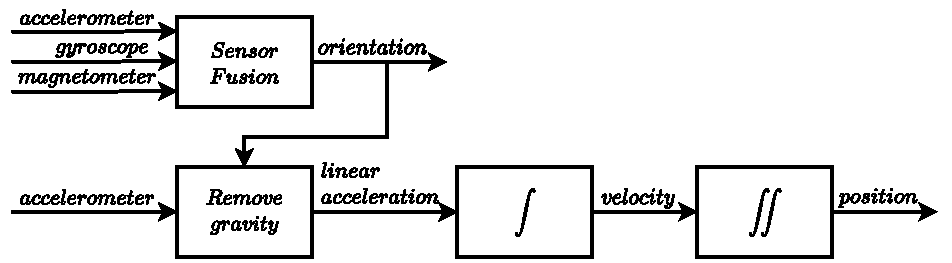
\includegraphics[width=0.9\textwidth]{figures/orientation_position.pdf}
    \caption{Overview of the position estimation method.}
    \label{fig:position}
\end{figure}

The next step consisted of experimentally testing the inertial system seeking to achieve position estimation merely by integrating the accelerometer measurements with the gravity compensation filter. Numerous experiments were performed in several settings. The tests involved walking on a straight line carrying a box containing the inertial system (with the inertial X-axis parallel to the path) for around 30 meters, evaluating the computed acceleration, velocity, and accumulative position estimation. Specific tests were executed at walking pace, others at running pace, and some with a combination of both.

% \begin{figure}[!h]
%     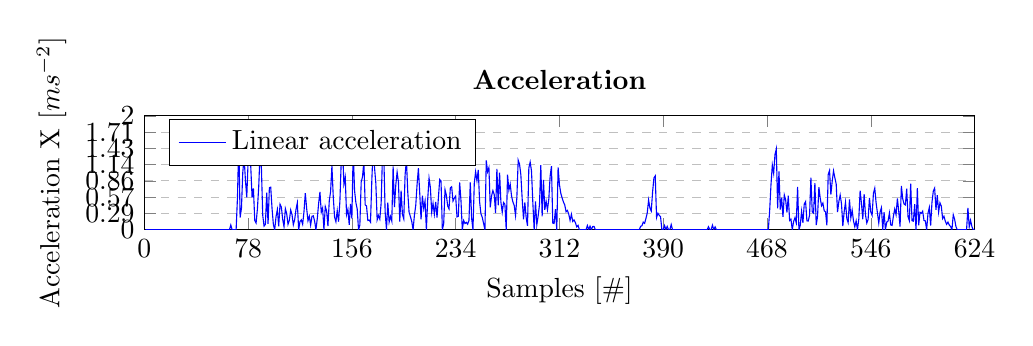
\begin{tikzpicture}
\begin{axis}[
    title={\textbf{Acceleration}},
    xlabel={Samples [\#] },
    ylabel={Acceleration X [$ms^{-2}$]},
    xmin=0, xmax=624,
    ymin=-0, ymax=2,
    xtick distance = 78,
    ytick distance=0.285,
    legend pos=north west,
    ymajorgrids=true,
    grid style=dashed,
    width = \linewidth,
	height = 0.25\textwidth,
]

\addplot[
    color=blue
    ]
    coordinates {
(1,0)
(2,0)
(3,0)
(4,0)
(5,0)
(6,0)
(7,0)
(8,0)
(9,0)
(10,0)
(11,0)
(12,0)
(13,0)
(14,0)
(15,0)
(16,0)
(17,0)
(18,0)
(19,0)
(20,0)
(21,0)
(22,0)
(23,0)
(24,0)
(25,0)
(26,0)
(27,0)
(28,0)
(29,0)
(30,0)
(31,0)
(32,0)
(33,0)
(34,0)
(35,0)
(36,0)
(37,0)
(38,0)
(39,0)
(40,0)
(41,0)
(42,0)
(43,0)
(44,0)
(45,0)
(46,0)
(47,0)
(48,0)
(49,0)
(50,0)
(51,0)
(52,0)
(53,0)
(54,0)
(55,0)
(56,0)
(57,0)
(58,0)
(59,0)
(60,0)
(61,0)
(62,0)
(63,0)
(64,0)
(65,0.08270433)
(66,0)
(67,0)
(68,0)
(69,0)
(70,0.5583076)
(71,1.560334)
(72,0.2115138)
(73,0.3759099)
(74,1.003705)
(75,1.270681)
(76,0.8640939)
(77,0.5691901)
(78,1.193927)
(79,1.363093)
(80,1.108371)
(81,0.5623293)
(82,0.7238063)
(83,0.1625629)
(84,0.118303)
(85,0.3652165)
(86,0.7613573)
(87,1.358668)
(88,1.085672)
(89,0.2515904)
(90,0.06395303)
(91,0.09338129)
(92,0.6505489)
(93,0.1030498)
(94,0.7363608)
(95,0.7458648)
(96,0.371991)
(97,0.09095393)
(98,0)
(99,0.2288308)
(100,0.3547924)
(101,0.06044533)
(102,0.4465622)
(103,0.3982781)
(104,0.1819616)
(105,0.05362022)
(106,0.3696096)
(107,0.283442)
(108,0.09497082)
(109,0.1625505)
(110,0.3459515)
(111,0.2673449)
(112,0.08692225)
(113,0.1770717)
(114,0.354268)
(115,0.4704921)
(116,0)
(117,0.1434379)
(118,0.1731488)
(119,0.09654384)
(120,0.3148962)
(121,0.6428003)
(122,0.3762831)
(123,0.1574949)
(124,0.2369482)
(125,0.08237637)
(126,0.2346799)
(127,0.2440059)
(128,0.1503531)
(129,0)
(130,0.1962429)
(131,0.4584124)
(132,0.663873)
(133,0.3070331)
(134,0.380938)
(135,0)
(136,0.4073497)
(137,0.3308759)
(138,0.06397649)
(139,0.5050195)
(140,0.6687342)
(141,1.117419)
(142,0.5784832)
(143,0.2216208)
(144,0.1397644)
(145,0.3358257)
(146,0.1410249)
(147,0.5008575)
(148,1.203228)
(149,1.416779)
(150,0.8025916)
(151,0.9253637)
(152,0.2635756)
(153,0.3567323)
(154,0.08751804)
(155,0.4515275)
(156,0.1968053)
(157,1.397453)
(158,0.6908656)
(159,0.4768153)
(160,0.3626091)
(161,0)
(162,0.08099926)
(163,0.8360435)
(164,0.9267252)
(165,1.204392)
(166,0.4355258)
(167,0.4168142)
(168,0.1631597)
(169,0.169665)
(170,0.1332702)
(171,0.8680125)
(172,1.459768)
(173,1.093511)
(174,0.8178315)
(175,0.17303)
(176,0.2480692)
(177,0.1857022)
(178,0.4677786)
(179,1.308649)
(180,1.292747)
(181,0.3130332)
(182,0)
(183,0.4754438)
(184,0.1338254)
(185,0.2338828)
(186,0.1513585)
(187,1.110016)
(188,0.3964491)
(189,0.7837675)
(190,1.008785)
(191,0.8363365)
(192,0.1441391)
(193,0.6848535)
(194,0.2684142)
(195,0.1896396)
(196,0.9659473)
(197,1.225042)
(198,0.6584739)
(199,0.3046332)
(200,0.2311385)
(201,0.1446532)
(202,0)
(203,0.2531439)
(204,0.4247202)
(205,0.7915803)
(206,1.076968)
(207,0.6393047)
(208,0.18045)
(209,0.5976918)
(210,0.3726646)
(211,0.5057043)
(212,0)
(213,0.5332688)
(214,0.9037191)
(215,0.7391905)
(216,0.3077584)
(217,0.4624692)
(218,0.271077)
(219,0.4853863)
(220,0.2142689)
(221,0.5487638)
(222,0.8800142)
(223,0.8549524)
(224,0)
(225,0.1044441)
(226,0.7028772)
(227,0.6064589)
(228,0.4182649)
(229,0.3660012)
(230,0.7349767)
(231,0.7531294)
(232,0.5032366)
(233,0.5549395)
(234,0.5897318)
(235,0.2255328)
(236,0.2354079)
(237,0.8293493)
(238,0.5110643)
(239,0)
(240,0.1626565)
(241,0.109669)
(242,0.1296327)
(243,0.09700366)
(244,0.1634522)
(245,0.8314447)
(246,0.2013358)
(247,0)
(248,0.8153185)
(249,1.016361)
(250,0.8605233)
(251,1.047545)
(252,0.4878371)
(253,0.2801501)
(254,0.2168312)
(255,0.1102494)
(256,0)
(257,1.215995)
(258,1.014892)
(259,1.089346)
(260,0.3929638)
(261,0.59536)
(262,0.685633)
(263,0.6145452)
(264,0.2930603)
(265,1.066259)
(266,0.4295098)
(267,1.002246)
(268,0.4866282)
(269,0.3064896)
(270,0.4760719)
(271,0.4470825)
(272,0)
(273,0.9670089)
(274,0.6932314)
(275,0.7976069)
(276,0.5921421)
(277,0.4884963)
(278,0.4271869)
(279,0.248104)
(280,0.5647231)
(281,1.2182)
(282,1.151464)
(283,0.9620384)
(284,0.5405983)
(285,0.1831884)
(286,0.4783494)
(287,0.2116105)
(288,0.06759779)
(289,1.082082)
(290,1.185404)
(291,1.029803)
(292,0.4793365)
(293,0)
(294,0.4975831)
(295,0.08786249)
(296,0.240528)
(297,0.4385661)
(298,1.133494)
(299,0.2344308)
(300,0.875211)
(301,0.348825)
(302,0.498484)
(303,0.3495025)
(304,0.5321168)
(305,0.9357553)
(306,1.113068)
(307,0.1169375)
(308,0.1092775)
(309,0.3613703)
(310,0)
(311,1.093161)
(312,0.7916846)
(313,0.6403999)
(314,0.5589567)
(315,0.4857246)
(316,0.4334849)
(317,0.3153615)
(318,0.338113)
(319,0.2731995)
(320,0.1628779)
(321,0.2712631)
(322,0.1449191)
(323,0.1721828)
(324,0.1242143)
(325,0.05079247)
(326,0.07711079)
(327,0)
(328,0)
(329,0)
(330,0)
(331,0)
(332,0)
(333,0.07397792)
(334,0)
(335,0.06348043)
(336,0)
(337,0.0558517)
(338,0.0577443)
(339,0)
(340,0)
(341,0)
(342,0)
(343,0)
(344,0)
(345,0)
(346,0)
(347,0)
(348,0)
(349,0)
(350,0)
(351,0)
(352,0)
(353,0)
(354,0)
(355,0)
(356,0)
(357,0)
(358,0)
(359,0)
(360,0)
(361,0)
(362,0)
(363,0)
(364,0)
(365,0)
(366,0)
(367,0)
(368,0)
(369,0)
(370,0)
(371,0)
(372,0)
(373,0.05847713)
(374,0.07048888)
(375,0.1339837)
(376,0.1124815)
(377,0.1951409)
(378,0.2948024)
(379,0.5195302)
(380,0.3810527)
(381,0.3264382)
(382,0.6576408)
(383,0.9059416)
(384,0.9425709)
(385,0.2140578)
(386,0.2894547)
(387,0.2521294)
(388,0.2275948)
(389,0)
(390,0)
(391,0.07377751)
(392,0)
(393,0.05839268)
(394,0)
(395,0)
(396,0.09107598)
(397,0)
(398,0)
(399,0)
(400,0)
(401,0)
(402,0)
(403,0)
(404,0)
(405,0)
(406,0)
(407,0)
(408,0)
(409,0)
(410,0)
(411,0)
(412,0)
(413,0)
(414,0)
(415,0)
(416,0)
(417,0)
(418,0)
(419,0)
(420,0)
(421,0)
(422,0)
(423,0)
(424,0.05228344)
(425,0)
(426,0)
(427,0.07947165)
(428,0)
(429,0.05000925)
(430,0)
(431,0)
(432,0)
(433,0)
(434,0)
(435,0)
(436,0)
(437,0)
(438,0)
(439,0)
(440,0)
(441,0)
(442,0)
(443,0)
(444,0)
(445,0)
(446,0)
(447,0)
(448,0)
(449,0)
(450,0)
(451,0)
(452,0)
(453,0)
(454,0)
(455,0)
(456,0)
(457,0)
(458,0)
(459,0)
(460,0)
(461,0)
(462,0)
(463,0)
(464,0)
(465,0)
(466,0)
(467,0)
(468,0)
(469,0)
(470,0.3337591)
(471,0.7904476)
(472,1.133774)
(473,0.9872878)
(474,1.316563)
(475,1.414771)
(476,0.3748502)
(477,1.021382)
(478,0.3534243)
(479,0.5635874)
(480,0.2261105)
(481,0.610221)
(482,0.525787)
(483,0.3030995)
(484,0.5952455)
(485,0.1626046)
(486,0.1853536)
(487,0)
(488,0.1426162)
(489,0.2093649)
(490,0.1207951)
(491,0.7487729)
(492,0)
(493,0.07739891)
(494,0.3237109)
(495,0.1220903)
(496,0.4493409)
(497,0.4923639)
(498,0.1561133)
(499,0.1526662)
(500,0.2537943)
(501,0.9147314)
(502,0.3125581)
(503,0.2889673)
(504,0.8176416)
(505,0.08093239)
(506,0.2350332)
(507,0.7472815)
(508,0.5535451)
(509,0.4206181)
(510,0.4677228)
(511,0.3327864)
(512,0.312816)
(513,0.07792404)
(514,0.9660884)
(515,1.037891)
(516,0.6155223)
(517,0.8470804)
(518,1.031141)
(519,0.9110786)
(520,0.8019853)
(521,0.3082083)
(522,0.4921479)
(523,0.6075731)
(524,0.4545872)
(525,0.06427832)
(526,0.3158281)
(527,0.4828798)
(528,0.196799)
(529,0.1264963)
(530,0.5315699)
(531,0.2063234)
(532,0.3443285)
(533,0.1552771)
(534,0.05246383)
(535,0.1564257)
(536,0)
(537,0.1873404)
(538,0.686246)
(539,0.4592639)
(540,0.1845886)
(541,0.6232172)
(542,0.2658765)
(543,0.1176916)
(544,0.1796833)
(545,0.5588526)
(546,0.3124085)
(547,0.2529012)
(548,0.6395702)
(549,0.7273252)
(550,0.4721871)
(551,0.2954658)
(552,0.1180191)
(553,0.3103034)
(554,0.3856865)
(555,0)
(556,0.3079722)
(557,0)
(558,0.1329881)
(559,0.1517593)
(560,0.2929947)
(561,0.08557587)
(562,0.07634291)
(563,0.2370027)
(564,0.3628211)
(565,0.264144)
(566,0.5468083)
(567,0.3280928)
(568,0.05574092)
(569,0.7659275)
(570,0.5446857)
(571,0.4490639)
(572,0.4343478)
(573,0.7181976)
(574,0.2264909)
(575,0.1594372)
(576,0.8067467)
(577,0.1595064)
(578,0.1501565)
(579,0.4477535)
(580,0)
(581,0.7302676)
(582,0.07700576)
(583,0.3053396)
(584,0.2875741)
(585,0.3242111)
(586,0.1623785)
(587,0.1548143)
(588,0)
(589,0.2885099)
(590,0.3903607)
(591,0.07102526)
(592,0.481882)
(593,0.6761222)
(594,0.728777)
(595,0.3481652)
(596,0.6048031)
(597,0.3090468)
(598,0.4714205)
(599,0.4147293)
(600,0.1967944)
(601,0.2369971)
(602,0.1512856)
(603,0.09513116)
(604,0.1339154)
(605,0.08336387)
(606,0.0561322)
(607,0)
(608,0.2625456)
(609,0.184552)
(610,0.0566308)
(611,0)
(612,0)
(613,0)
(614,0)
(615,0)
(616,0)
(617,0)
(618,0)
(619,0.3846283)
(620,0.05054063)
(621,0.165349)
(622,0.0548058)
(623,0)
(624,0)
};
    \addlegendentry{Linear acceleration }
    

\end{axis}
\end{tikzpicture}
%     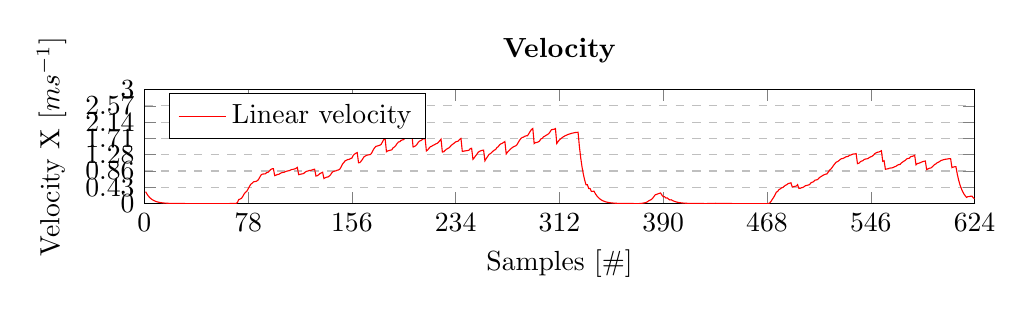
\begin{tikzpicture}
\begin{axis}[
    title={\textbf{Velocity}},
    xlabel={Samples [\#] },
    ylabel={Velocity X [$ms^{-1}$]},
    xmin=0, xmax=624,
    ymin=-0, ymax=3,
    xtick distance = 78,
    ytick distance = 0.428,
    legend pos=north west,
    ymajorgrids=true,
    grid style=dashed,
    width = \linewidth,
	height = 0.25\textwidth,
]
\addplot[
    color=red
    ]
    coordinates {
    (1,0.3123816)
(2,0.2499053)
(3,0.1999242)
(4,0.1599394)
(5,0.1279515)
(6,0.1023612)
(7,0.08188897)
(8,0.06551117)
(9,0.05240894)
(10,0.04192716)
(11,0.03354172)
(12,0.02683338)
(13,0.0214667)
(14,0.01717336)
(15,0.01373869)
(16,0.01099095)
(17,0.008792763)
(18,0.00703421)
(19,0.005627368)
(20,0.004501895)
(21,0.003601516)
(22,0.002881212)
(23,0.00230497)
(24,0.001843976)
(25,0.001475181)
(26,0.001180145)
(27,0.0009441158)
(28,0.0007552927)
(29,0.0006042341)
(30,0.0004833873)
(31,0.0003867098)
(32,0.0003093679)
(33,0.0002474943)
(34,0.0001979954)
(35,0.0001583964)
(36,0.0001267171)
(37,0.0001013737)
(38,0.00008109894)
(39,0.00006487916)
(40,0.00005190332)
(41,0.00004152266)
(42,0.00003321813)
(43,0.0000265745)
(44,0.0000212596)
(45,0.00001700768)
(46,0.00001360615)
(47,0.00001088492)
(48,0.000008707934)
(49,0.000006966347)
(50,0.000005573078)
(51,0.000004458463)
(52,0.00000356677)
(53,0.000002853416)
(54,0.000002282733)
(55,0.000001826186)
(56,0.000001460949)
(57,0.000001168759)
(58,0.0000009350075)
(59,0.0000007480061)
(60,0.0000005984048)
(61,0.0000004787238)
(62,0.0000003829791)
(63,0.0000003063833)
(64,0.0000002451066)
(65,0.004135461)
(66,0.003308369)
(67,0.002646696)
(68,0.002117357)
(69,0.001693885)
(70,0.02960926)
(71,0.107626)
(72,0.1182016)
(73,0.1369972)
(74,0.1871824)
(75,0.2507164)
(76,0.2939211)
(77,0.3223807)
(78,0.382077)
(79,0.4502316)
(80,0.5056502)
(81,0.5337667)
(82,0.569957)
(83,0.5780852)
(84,0.5840003)
(85,0.6022612)
(86,0.6403291)
(87,0.7082624)
(88,0.7625461)
(89,0.7751256)
(90,0.7783232)
(91,0.7829923)
(92,0.8155197)
(93,0.8206722)
(94,0.8574903)
(95,0.8947835)
(96,0.9133831)
(97,0.9179308)
(98,0.7343447)
(99,0.7457862)
(100,0.7635258)
(101,0.7665481)
(102,0.7888762)
(103,0.8087901)
(104,0.8178882)
(105,0.8205691)
(106,0.8390496)
(107,0.8532217)
(108,0.8579702)
(109,0.8660977)
(110,0.8833953)
(111,0.8967626)
(112,0.9011086)
(113,0.9099623)
(114,0.9276757)
(115,0.9512003)
(116,0.7609603)
(117,0.7681322)
(118,0.7767896)
(119,0.7816168)
(120,0.7973616)
(121,0.8295016)
(122,0.8483158)
(123,0.8561905)
(124,0.868038)
(125,0.8721567)
(126,0.8838907)
(127,0.8960911)
(128,0.9036087)
(129,0.722887)
(130,0.7326992)
(131,0.7556198)
(132,0.7888134)
(133,0.8041651)
(134,0.823212)
(135,0.6585696)
(136,0.6789371)
(137,0.6954809)
(138,0.6986797)
(139,0.7239306)
(140,0.7573674)
(141,0.8132383)
(142,0.8421625)
(143,0.8532435)
(144,0.8602318)
(145,0.877023)
(146,0.8840743)
(147,0.9091171)
(148,0.9692785)
(149,1.040118)
(150,1.080247)
(151,1.126515)
(152,1.139694)
(153,1.157531)
(154,1.161907)
(155,1.184483)
(156,1.194323)
(157,1.264196)
(158,1.298739)
(159,1.32258)
(160,1.34071)
(161,1.072568)
(162,1.076618)
(163,1.11842)
(164,1.164757)
(165,1.224976)
(166,1.246753)
(167,1.267594)
(168,1.275751)
(169,1.284235)
(170,1.290898)
(171,1.334299)
(172,1.407287)
(173,1.461963)
(174,1.502854)
(175,1.511506)
(176,1.523909)
(177,1.533195)
(178,1.556583)
(179,1.622016)
(180,1.686653)
(181,1.702305)
(182,1.361844)
(183,1.385616)
(184,1.392307)
(185,1.404002)
(186,1.411569)
(187,1.46707)
(188,1.486893)
(189,1.526081)
(190,1.57652)
(191,1.618337)
(192,1.625544)
(193,1.659787)
(194,1.673208)
(195,1.68269)
(196,1.730987)
(197,1.792239)
(198,1.825163)
(199,1.840394)
(200,1.851951)
(201,1.859184)
(202,1.487347)
(203,1.500004)
(204,1.52124)
(205,1.56082)
(206,1.614668)
(207,1.646633)
(208,1.655656)
(209,1.68554)
(210,1.704173)
(211,1.729459)
(212,1.383567)
(213,1.41023)
(214,1.455416)
(215,1.492376)
(216,1.507764)
(217,1.530887)
(218,1.544441)
(219,1.56871)
(220,1.579424)
(221,1.606862)
(222,1.650863)
(223,1.69361)
(224,1.354888)
(225,1.360111)
(226,1.395254)
(227,1.425577)
(228,1.446491)
(229,1.464791)
(230,1.501539)
(231,1.539196)
(232,1.564358)
(233,1.592105)
(234,1.621591)
(235,1.632868)
(236,1.644638)
(237,1.686106)
(238,1.711659)
(239,1.369327)
(240,1.37746)
(241,1.382943)
(242,1.389425)
(243,1.394275)
(244,1.402448)
(245,1.44402)
(246,1.454087)
(247,1.163269)
(248,1.204035)
(249,1.254853)
(250,1.29788)
(251,1.350257)
(252,1.374649)
(253,1.388656)
(254,1.399498)
(255,1.40501)
(256,1.124008)
(257,1.184808)
(258,1.235552)
(259,1.29002)
(260,1.309668)
(261,1.339436)
(262,1.373718)
(263,1.404445)
(264,1.419098)
(265,1.472411)
(266,1.493886)
(267,1.543998)
(268,1.56833)
(269,1.583654)
(270,1.607458)
(271,1.629812)
(272,1.30385)
(273,1.3522)
(274,1.386862)
(275,1.426742)
(276,1.456349)
(277,1.480774)
(278,1.502133)
(279,1.514538)
(280,1.542774)
(281,1.603684)
(282,1.661258)
(283,1.70936)
(284,1.736389)
(285,1.745549)
(286,1.769466)
(287,1.780047)
(288,1.783427)
(289,1.837531)
(290,1.896801)
(291,1.948291)
(292,1.972258)
(293,1.577806)
(294,1.602686)
(295,1.607079)
(296,1.619105)
(297,1.641033)
(298,1.697708)
(299,1.70943)
(300,1.75319)
(301,1.770631)
(302,1.795556)
(303,1.813031)
(304,1.839637)
(305,1.886424)
(306,1.942078)
(307,1.947925)
(308,1.953388)
(309,1.971457)
(310,1.577166)
(311,1.631824)
(312,1.671408)
(313,1.703428)
(314,1.731376)
(315,1.755662)
(316,1.777336)
(317,1.793104)
(318,1.81001)
(319,1.82367)
(320,1.831814)
(321,1.845377)
(322,1.852623)
(323,1.861232)
(324,1.867443)
(325,1.869982)
(326,1.873838)
(327,1.49907)
(328,1.199256)
(329,0.959405)
(330,0.7675241)
(331,0.6140193)
(332,0.4912154)
(333,0.4949143)
(334,0.3959315)
(335,0.3991055)
(336,0.3192844)
(337,0.322077)
(338,0.3249642)
(339,0.2599714)
(340,0.2079771)
(341,0.1663817)
(342,0.1331053)
(343,0.1064843)
(344,0.08518743)
(345,0.06814995)
(346,0.05451996)
(347,0.04361597)
(348,0.03489277)
(349,0.02791422)
(350,0.02233138)
(351,0.0178651)
(352,0.01429208)
(353,0.01143367)
(354,0.009146934)
(355,0.007317547)
(356,0.005854037)
(357,0.00468323)
(358,0.003746584)
(359,0.002997267)
(360,0.002397814)
(361,0.001918251)
(362,0.001534601)
(363,0.001227681)
(364,0.0009821445)
(365,0.0007857157)
(366,0.0006285727)
(367,0.0005028581)
(368,0.0004022865)
(369,0.0003218292)
(370,0.0002574634)
(371,0.0002059707)
(372,0.0001647766)
(373,0.003088633)
(374,0.006613077)
(375,0.01331226)
(376,0.01893634)
(377,0.02869339)
(378,0.0434335)
(379,0.06941001)
(380,0.08846265)
(381,0.1047846)
(382,0.1376666)
(383,0.1829637)
(384,0.2300922)
(385,0.2407951)
(386,0.2552679)
(387,0.2678743)
(388,0.2792541)
(389,0.2234033)
(390,0.1787226)
(391,0.1824115)
(392,0.1459292)
(393,0.1488488)
(394,0.1190791)
(395,0.09526324)
(396,0.09981705)
(397,0.07985364)
(398,0.06388291)
(399,0.05110633)
(400,0.04088506)
(401,0.03270805)
(402,0.02616644)
(403,0.02093315)
(404,0.01674652)
(405,0.01339722)
(406,0.01071778)
(407,0.008574221)
(408,0.006859376)
(409,0.005487501)
(410,0.004390001)
(411,0.003512001)
(412,0.002809601)
(413,0.002247681)
(414,0.001798145)
(415,0.001438516)
(416,0.001150813)
(417,0.00092065)
(418,0.0007365201)
(419,0.000589216)
(420,0.0004713729)
(421,0.0003770983)
(422,0.0003016786)
(423,0.0002413429)
(424,0.002855515)
(425,0.002284412)
(426,0.00182753)
(427,0.005801112)
(428,0.00464089)
(429,0.007141353)
(430,0.005713082)
(431,0.004570466)
(432,0.003656373)
(433,0.002925098)
(434,0.002340079)
(435,0.001872063)
(436,0.00149765)
(437,0.00119812)
(438,0.0009584963)
(439,0.000766797)
(440,0.0006134377)
(441,0.0004907501)
(442,0.0003926001)
(443,0.0003140801)
(444,0.0002512641)
(445,0.0002010113)
(446,0.000160809)
(447,0.0001286472)
(448,0.0001029178)
(449,0.00008233422)
(450,0.00006586738)
(451,0.0000526939)
(452,0.00004215512)
(453,0.0000337241)
(454,0.00002697928)
(455,0.00002158342)
(456,0.00001726674)
(457,0.00001381339)
(458,0.00001105071)
(459,0.00000884057)
(460,0.000007072456)
(461,0.000005657966)
(462,0.000004526372)
(463,0.000003621098)
(464,0.000002896878)
(465,0.000002317503)
(466,0.000001854002)
(467,0.000001483202)
(468,0.000001186561)
(469,0.0000009492492)
(470,0.01668891)
(471,0.05621129)
(472,0.1129)
(473,0.1622643)
(474,0.2280925)
(475,0.298831)
(476,0.3175735)
(477,0.3686427)
(478,0.3863139)
(479,0.4144932)
(480,0.4257987)
(481,0.4563098)
(482,0.4825992)
(483,0.4977541)
(484,0.5275164)
(485,0.5356467)
(486,0.5449143)
(487,0.4359315)
(488,0.4430623)
(489,0.4535306)
(490,0.4595703)
(491,0.497009)
(492,0.3976072)
(493,0.4014771)
(494,0.4176627)
(495,0.4237672)
(496,0.4462343)
(497,0.4708524)
(498,0.4786581)
(499,0.4862914)
(500,0.4989811)
(501,0.5447177)
(502,0.5603456)
(503,0.5747939)
(504,0.615676)
(505,0.6197227)
(506,0.6314743)
(507,0.6688384)
(508,0.6965156)
(509,0.7175465)
(510,0.7409327)
(511,0.7575719)
(512,0.7732127)
(513,0.7771089)
(514,0.8254133)
(515,0.8773079)
(516,0.908084)
(517,0.9504381)
(518,1.001995)
(519,1.047549)
(520,1.087648)
(521,1.103059)
(522,1.127666)
(523,1.158045)
(524,1.180774)
(525,1.183988)
(526,1.19978)
(527,1.223923)
(528,1.233763)
(529,1.240088)
(530,1.266667)
(531,1.276983)
(532,1.294199)
(533,1.301963)
(534,1.304586)
(535,1.312408)
(536,1.049926)
(537,1.059293)
(538,1.093605)
(539,1.116569)
(540,1.125798)
(541,1.156959)
(542,1.170253)
(543,1.176137)
(544,1.185121)
(545,1.213064)
(546,1.228685)
(547,1.24133)
(548,1.273308)
(549,1.309674)
(550,1.333284)
(551,1.348057)
(552,1.353958)
(553,1.369473)
(554,1.388757)
(555,1.111006)
(556,1.126405)
(557,0.9011237)
(558,0.9077731)
(559,0.915361)
(560,0.9300108)
(561,0.9342896)
(562,0.9381067)
(563,0.9499568)
(564,0.9680979)
(565,0.981305)
(566,1.008646)
(567,1.02505)
(568,1.027837)
(569,1.066133)
(570,1.093368)
(571,1.115821)
(572,1.137538)
(573,1.173448)
(574,1.184773)
(575,1.192745)
(576,1.233082)
(577,1.241057)
(578,1.248565)
(579,1.270953)
(580,1.016762)
(581,1.053276)
(582,1.057126)
(583,1.072393)
(584,1.086772)
(585,1.102982)
(586,1.111101)
(587,1.118842)
(588,0.8950734)
(589,0.909499)
(590,0.929017)
(591,0.9325682)
(592,0.9566623)
(593,0.9904684)
(594,1.026907)
(595,1.044315)
(596,1.074556)
(597,1.090008)
(598,1.113579)
(599,1.134315)
(600,1.144155)
(601,1.156005)
(602,1.163569)
(603,1.168326)
(604,1.175022)
(605,1.17919)
(606,1.181997)
(607,0.9455973)
(608,0.9587246)
(609,0.9679522)
(610,0.9707836)
(611,0.776627)
(612,0.6213016)
(613,0.4970413)
(614,0.3976331)
(615,0.3181064)
(616,0.2544852)
(617,0.2035881)
(618,0.1628705)
(619,0.1821019)
(620,0.184629)
(621,0.1928964)
(622,0.1956367)
(623,0.1565094)
(624,0.1252075)
};
    \addlegendentry{Linear velocity}

\end{axis}
\end{tikzpicture}
%     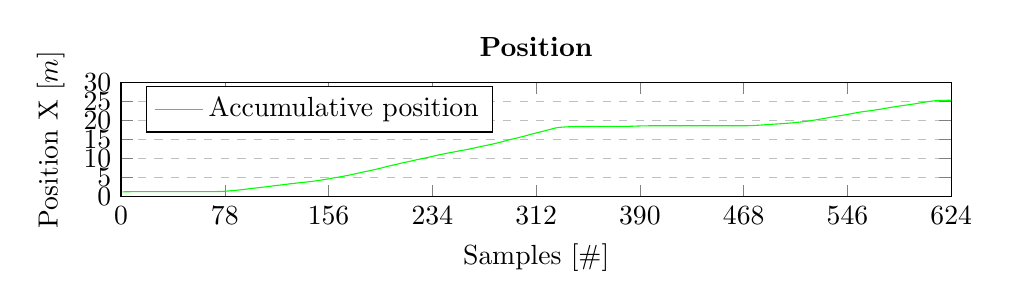
\begin{tikzpicture}
\begin{axis}[
    title={\textbf{Position }},
    xlabel={Samples [\#] },
    ylabel={Position X [$m$]},
    xmin=0, xmax=624,
    ymin=-0, ymax=30,
    xtick distance = 78,
    ytick={0,5,10,15,20,25,30},
    legend pos=north west,
    ymajorgrids=true,
    grid style=dashed,
    width = \linewidth,
	height = 0.25\textwidth,
]
\addplot[
    color=green
    ]
    coordinates {
    (1,1.256727)
(2,1.269222)
(3,1.279218)
(4,1.287215)
(5,1.293613)
(6,1.298731)
(7,1.302825)
(8,1.306101)
(9,1.308721)
(10,1.310818)
(11,1.312495)
(12,1.313836)
(13,1.31491)
(14,1.315768)
(15,1.316455)
(16,1.317005)
(17,1.317444)
(18,1.317796)
(19,1.318077)
(20,1.318303)
(21,1.318483)
(22,1.318627)
(23,1.318742)
(24,1.318834)
(25,1.318908)
(26,1.318967)
(27,1.319014)
(28,1.319052)
(29,1.319082)
(30,1.319106)
(31,1.319126)
(32,1.319141)
(33,1.319153)
(34,1.319163)
(35,1.319171)
(36,1.319178)
(37,1.319183)
(38,1.319187)
(39,1.31919)
(40,1.319193)
(41,1.319195)
(42,1.319196)
(43,1.319198)
(44,1.319199)
(45,1.319199)
(46,1.3192)
(47,1.319201)
(48,1.319201)
(49,1.319202)
(50,1.319202)
(51,1.319202)
(52,1.319202)
(53,1.319202)
(54,1.319202)
(55,1.319203)
(56,1.319203)
(57,1.319203)
(58,1.319203)
(59,1.319203)
(60,1.319203)
(61,1.319203)
(62,1.319203)
(63,1.319203)
(64,1.319203)
(65,1.319513)
(66,1.319678)
(67,1.319811)
(68,1.319916)
(69,1.320001)
(70,1.322179)
(71,1.329511)
(72,1.335686)
(73,1.343005)
(74,1.353619)
(75,1.367743)
(76,1.383519)
(77,1.40035)
(78,1.420946)
(79,1.445162)
(80,1.47183)
(81,1.499221)
(82,1.528623)
(83,1.557731)
(84,1.587079)
(85,1.617648)
(86,1.650617)
(87,1.687728)
(88,1.727212)
(89,1.766283)
(90,1.805279)
(91,1.844545)
(92,1.886135)
(93,1.927297)
(94,1.971092)
(95,2.016763)
(96,2.062898)
(97,2.108908)
(98,2.145625)
(99,2.1832)
(100,2.22182)
(101,2.260223)
(102,2.300225)
(103,2.341163)
(104,2.382285)
(105,2.42338)
(106,2.465795)
(107,2.50881)
(108,2.551827)
(109,2.595335)
(110,2.639937)
(111,2.68511)
(112,2.730274)
(113,2.775993)
(114,2.82282)
(115,2.870968)
(116,2.909016)
(117,2.947602)
(118,2.986658)
(119,3.025859)
(120,3.066121)
(121,3.108399)
(122,3.151286)
(123,3.194292)
(124,3.23799)
(125,3.281701)
(126,3.326189)
(127,3.371298)
(128,3.416667)
(129,3.452811)
(130,3.489691)
(131,3.528045)
(132,3.568316)
(133,3.608908)
(134,3.650544)
(135,3.683473)
(136,3.717929)
(137,3.753117)
(138,3.788131)
(139,3.824958)
(140,3.863663)
(141,3.905721)
(142,3.948553)
(143,3.991492)
(144,4.034678)
(145,4.078949)
(146,4.123329)
(147,4.169411)
(148,4.219379)
(149,4.273156)
(150,4.328171)
(151,4.385653)
(152,4.442968)
(153,4.50129)
(154,4.559495)
(155,4.619284)
(156,4.679246)
(157,4.744203)
(158,4.810003)
(159,4.876728)
(160,4.944217)
(161,4.997845)
(162,5.051777)
(163,5.108744)
(164,5.16814)
(165,5.230894)
(166,5.293776)
(167,5.357677)
(168,5.421668)
(169,5.486092)
(170,5.550804)
(171,5.618604)
(172,5.690793)
(173,5.765258)
(174,5.841423)
(175,5.917214)
(176,5.99372)
(177,6.070612)
(178,6.149026)
(179,6.231762)
(180,6.317711)
(181,6.403217)
(182,6.47131)
(183,6.541185)
(184,6.610968)
(185,6.68146)
(186,6.752228)
(187,6.826969)
(188,6.901809)
(189,6.979093)
(190,7.05918)
(191,7.141142)
(192,7.2226)
(193,7.306445)
(194,7.390441)
(195,7.474813)
(196,7.562569)
(197,7.653712)
(198,7.745793)
(199,7.838194)
(200,7.93108)
(201,8.02422)
(202,8.098588)
(203,8.173904)
(204,8.250498)
(205,8.329528)
(206,8.411608)
(207,8.494739)
(208,8.577747)
(209,8.662771)
(210,8.748446)
(211,8.83555)
(212,8.904729)
(213,8.975907)
(214,9.049808)
(215,9.12535)
(216,9.201123)
(217,9.278246)
(218,9.355806)
(219,9.434849)
(220,9.514088)
(221,9.595117)
(222,9.67876)
(223,9.764509)
(224,9.832253)
(225,9.90039)
(226,9.971031)
(227,10.04307)
(228,10.11592)
(229,10.18961)
(230,10.26561)
(231,10.34351)
(232,10.42236)
(233,10.50266)
(234,10.58447)
(235,10.6664)
(236,10.74892)
(237,10.83427)
(238,10.92049)
(239,10.98895)
(240,11.05803)
(241,11.12731)
(242,11.19695)
(243,11.26678)
(244,11.33711)
(245,11.41035)
(246,11.48331)
(247,11.54147)
(248,11.60269)
(249,11.6667)
(250,11.73267)
(251,11.8015)
(252,11.87084)
(253,11.94062)
(254,12.01087)
(255,12.08126)
(256,12.13746)
(257,12.19822)
(258,12.26126)
(259,12.32713)
(260,12.3931)
(261,12.46082)
(262,12.53036)
(263,12.60135)
(264,12.67267)
(265,12.74762)
(266,12.82286)
(267,12.90131)
(268,12.98033)
(269,13.0599)
(270,13.14087)
(271,13.22292)
(272,13.28811)
(273,13.35693)
(274,13.42714)
(275,13.49947)
(276,13.57303)
(277,13.64768)
(278,13.72332)
(279,13.79936)
(280,13.8772)
(281,13.95891)
(282,14.04341)
(283,14.13008)
(284,14.21758)
(285,14.30508)
(286,14.39415)
(287,14.48342)
(288,14.57268)
(289,14.6659)
(290,14.76223)
(291,14.86093)
(292,14.96014)
(293,15.03903)
(294,15.11979)
(295,15.20025)
(296,15.28151)
(297,15.36411)
(298,15.45041)
(299,15.53617)
(300,15.62493)
(301,15.71389)
(302,15.80429)
(303,15.89538)
(304,15.98803)
(305,16.08352)
(306,16.18201)
(307,16.27956)
(308,16.37736)
(309,16.47639)
(310,16.55524)
(311,16.6382)
(312,16.72276)
(313,16.80873)
(314,16.896)
(315,16.98439)
(316,17.0738)
(317,17.16385)
(318,17.25477)
(319,17.3463)
(320,17.43809)
(321,17.5307)
(322,17.62351)
(323,17.71679)
(324,17.81032)
(325,17.90388)
(326,17.99767)
(327,18.07262)
(328,18.13258)
(329,18.18055)
(330,18.21893)
(331,18.24963)
(332,18.27419)
(333,18.29903)
(334,18.31882)
(335,18.33886)
(336,18.35483)
(337,18.371)
(338,18.38732)
(339,18.40032)
(340,18.41072)
(341,18.41904)
(342,18.42569)
(343,18.43102)
(344,18.43527)
(345,18.43868)
(346,18.44141)
(347,18.44359)
(348,18.44533)
(349,18.44673)
(350,18.44785)
(351,18.44874)
(352,18.44945)
(353,18.45003)
(354,18.45048)
(355,18.45085)
(356,18.45114)
(357,18.45138)
(358,18.45156)
(359,18.45171)
(360,18.45183)
(361,18.45193)
(362,18.45201)
(363,18.45207)
(364,18.45212)
(365,18.45216)
(366,18.45219)
(367,18.45221)
(368,18.45223)
(369,18.45225)
(370,18.45226)
(371,18.45227)
(372,18.45228)
(373,18.45251)
(374,18.45292)
(375,18.45376)
(376,18.45485)
(377,18.45652)
(378,18.45906)
(379,18.46318)
(380,18.46808)
(381,18.47373)
(382,18.48144)
(383,18.49172)
(384,18.5044)
(385,18.51671)
(386,18.52983)
(387,18.54354)
(388,18.55779)
(389,18.56896)
(390,18.57789)
(391,18.58711)
(392,18.5944)
(393,18.60192)
(394,18.60787)
(395,18.61263)
(396,18.61774)
(397,18.62173)
(398,18.62493)
(399,18.62748)
(400,18.62953)
(401,18.63116)
(402,18.63247)
(403,18.63352)
(404,18.63435)
(405,18.63502)
(406,18.63556)
(407,18.63599)
(408,18.63633)
(409,18.63661)
(410,18.63683)
(411,18.637)
(412,18.63714)
(413,18.63726)
(414,18.63734)
(415,18.63742)
(416,18.63748)
(417,18.63752)
(418,18.63756)
(419,18.63758)
(420,18.63761)
(421,18.63763)
(422,18.63764)
(423,18.63765)
(424,18.63786)
(425,18.63798)
(426,18.63807)
(427,18.63846)
(428,18.63869)
(429,18.63911)
(430,18.63939)
(431,18.63962)
(432,18.63981)
(433,18.63995)
(434,18.64007)
(435,18.64016)
(436,18.64024)
(437,18.6403)
(438,18.64035)
(439,18.64038)
(440,18.64041)
(441,18.64044)
(442,18.64046)
(443,18.64047)
(444,18.64049)
(445,18.6405)
(446,18.6405)
(447,18.64051)
(448,18.64051)
(449,18.64052)
(450,18.64052)
(451,18.64052)
(452,18.64053)
(453,18.64053)
(454,18.64053)
(455,18.64053)
(456,18.64053)
(457,18.64053)
(458,18.64053)
(459,18.64053)
(460,18.64053)
(461,18.64053)
(462,18.64053)
(463,18.64053)
(464,18.64053)
(465,18.64053)
(466,18.64053)
(467,18.64053)
(468,18.64053)
(469,18.64053)
(470,18.64178)
(471,18.64558)
(472,18.65265)
(473,18.66199)
(474,18.67504)
(475,18.69175)
(476,18.7081)
(477,18.72781)
(478,18.74757)
(479,18.769)
(480,18.79057)
(481,18.81415)
(482,18.83894)
(483,18.8642)
(484,18.89132)
(485,18.91831)
(486,18.94579)
(487,18.96758)
(488,18.98991)
(489,19.01285)
(490,19.03598)
(491,19.06177)
(492,19.08165)
(493,19.10182)
(494,19.12311)
(495,19.14445)
(496,19.16732)
(497,19.19148)
(498,19.21561)
(499,19.24011)
(500,19.26538)
(501,19.29376)
(502,19.32217)
(503,19.35127)
(504,19.38307)
(505,19.41416)
(506,19.44603)
(507,19.48041)
(508,19.51592)
(509,19.55233)
(510,19.58996)
(511,19.62825)
(512,19.6673)
(513,19.70626)
(514,19.74874)
(515,19.7939)
(516,19.84007)
(517,19.88865)
(518,19.94004)
(519,19.99356)
(520,20.04894)
(521,20.10448)
(522,20.16148)
(523,20.22014)
(524,20.27975)
(525,20.33903)
(526,20.39941)
(527,20.46121)
(528,20.52315)
(529,20.58531)
(530,20.64931)
(531,20.71341)
(532,20.77855)
(533,20.84385)
(534,20.90914)
(535,20.97496)
(536,21.02745)
(537,21.08065)
(538,21.13619)
(539,21.19259)
(540,21.24911)
(541,21.30774)
(542,21.36658)
(543,21.42554)
(544,21.48502)
(545,21.54637)
(546,21.6082)
(547,21.67058)
(548,21.73504)
(549,21.80143)
(550,21.86869)
(551,21.93646)
(552,22.00431)
(553,22.07317)
(554,22.14309)
(555,22.19864)
(556,22.25534)
(557,22.3004)
(558,22.34595)
(559,22.39191)
(560,22.43878)
(561,22.4856)
(562,22.5326)
(563,22.58039)
(564,22.62925)
(565,22.67865)
(566,22.72976)
(567,22.78143)
(568,22.83289)
(569,22.88715)
(570,22.9425)
(571,22.99886)
(572,23.05628)
(573,23.11584)
(574,23.17537)
(575,23.2352)
(576,23.29787)
(577,23.36012)
(578,23.42273)
(579,23.48684)
(580,23.53768)
(581,23.59126)
(582,23.64421)
(583,23.69821)
(584,23.75291)
(585,23.80847)
(586,23.86422)
(587,23.92036)
(588,23.96511)
(589,24.01095)
(590,24.05788)
(591,24.1046)
(592,24.15304)
(593,24.20341)
(594,24.25566)
(595,24.30831)
(596,24.3628)
(597,24.41768)
(598,24.47395)
(599,24.53118)
(600,24.58864)
(601,24.64673)
(602,24.7051)
(603,24.76363)
(604,24.82255)
(605,24.88162)
(606,24.94078)
(607,24.98806)
(608,25.03633)
(609,25.08496)
(610,25.13357)
(611,25.1724)
(612,25.20346)
(613,25.22832)
(614,25.2482)
(615,25.2641)
(616,25.27683)
(617,25.28701)
(618,25.29515)
(619,25.30474)
(620,25.31403)
(621,25.32388)
(622,25.33373)
(623,25.34156)
(624,25.34782)
};
    \addlegendentry{ Accumulative position}

\end{axis}
\end{tikzpicture}


%     \caption{Experiment conducted with X-axis only accelerometer measurement with gravity compensation. Carrying the INS torso height through 30 meters straight and briefly stopping halfway. }
%     \label{fig:1dimension}
% \end{figure}

\begin{figure}[!h]
    \centering
    \resizebox{1\linewidth}{!}{%% Creator: Matplotlib, PGF backend
%%
%% To include the figure in your LaTeX document, write
%%   \input{<filename>.pgf}
%%
%% Make sure the required packages are loaded in your preamble
%%   \usepackage{pgf}
%%
%% and, on pdftex
%%   \usepackage[utf8]{inputenc}\DeclareUnicodeCharacter{2212}{-}
%%
%% or, on luatex and xetex
%%   \usepackage{unicode-math}
%%
%% Figures using additional raster images can only be included by \input if
%% they are in the same directory as the main LaTeX file. For loading figures
%% from other directories you can use the `import` package
%%   \usepackage{import}
%%
%% and then include the figures with
%%   \import{<path to file>}{<filename>.pgf}
%%
%% Matplotlib used the following preamble
%%   \usepackage{fontspec}
%%
\begingroup%
\makeatletter%
\begin{pgfpicture}%
\pgfpathrectangle{\pgfpointorigin}{\pgfqpoint{6.400000in}{4.800000in}}%
\pgfusepath{use as bounding box, clip}%
\begin{pgfscope}%
\pgfsetbuttcap%
\pgfsetmiterjoin%
\definecolor{currentfill}{rgb}{1.000000,1.000000,1.000000}%
\pgfsetfillcolor{currentfill}%
\pgfsetlinewidth{0.000000pt}%
\definecolor{currentstroke}{rgb}{1.000000,1.000000,1.000000}%
\pgfsetstrokecolor{currentstroke}%
\pgfsetdash{}{0pt}%
\pgfpathmoveto{\pgfqpoint{0.000000in}{0.000000in}}%
\pgfpathlineto{\pgfqpoint{6.400000in}{0.000000in}}%
\pgfpathlineto{\pgfqpoint{6.400000in}{4.800000in}}%
\pgfpathlineto{\pgfqpoint{0.000000in}{4.800000in}}%
\pgfpathclose%
\pgfusepath{fill}%
\end{pgfscope}%
\begin{pgfscope}%
\pgfsetbuttcap%
\pgfsetmiterjoin%
\definecolor{currentfill}{rgb}{1.000000,1.000000,1.000000}%
\pgfsetfillcolor{currentfill}%
\pgfsetlinewidth{0.000000pt}%
\definecolor{currentstroke}{rgb}{0.000000,0.000000,0.000000}%
\pgfsetstrokecolor{currentstroke}%
\pgfsetstrokeopacity{0.000000}%
\pgfsetdash{}{0pt}%
\pgfpathmoveto{\pgfqpoint{0.580556in}{3.665000in}}%
\pgfpathlineto{\pgfqpoint{6.250000in}{3.665000in}}%
\pgfpathlineto{\pgfqpoint{6.250000in}{4.451000in}}%
\pgfpathlineto{\pgfqpoint{0.580556in}{4.451000in}}%
\pgfpathclose%
\pgfusepath{fill}%
\end{pgfscope}%
\begin{pgfscope}%
\pgfsetbuttcap%
\pgfsetroundjoin%
\definecolor{currentfill}{rgb}{0.000000,0.000000,0.000000}%
\pgfsetfillcolor{currentfill}%
\pgfsetlinewidth{0.803000pt}%
\definecolor{currentstroke}{rgb}{0.000000,0.000000,0.000000}%
\pgfsetstrokecolor{currentstroke}%
\pgfsetdash{}{0pt}%
\pgfsys@defobject{currentmarker}{\pgfqpoint{0.000000in}{-0.048611in}}{\pgfqpoint{0.000000in}{0.000000in}}{%
\pgfpathmoveto{\pgfqpoint{0.000000in}{0.000000in}}%
\pgfpathlineto{\pgfqpoint{0.000000in}{-0.048611in}}%
\pgfusepath{stroke,fill}%
}%
\begin{pgfscope}%
\pgfsys@transformshift{0.838258in}{3.665000in}%
\pgfsys@useobject{currentmarker}{}%
\end{pgfscope}%
\end{pgfscope}%
\begin{pgfscope}%
\definecolor{textcolor}{rgb}{0.000000,0.000000,0.000000}%
\pgfsetstrokecolor{textcolor}%
\pgfsetfillcolor{textcolor}%
\pgftext[x=0.838258in,y=3.567777in,,top]{\color{textcolor}\rmfamily\fontsize{10.000000}{12.000000}\selectfont \(\displaystyle {0}\)}%
\end{pgfscope}%
\begin{pgfscope}%
\pgfsetbuttcap%
\pgfsetroundjoin%
\definecolor{currentfill}{rgb}{0.000000,0.000000,0.000000}%
\pgfsetfillcolor{currentfill}%
\pgfsetlinewidth{0.803000pt}%
\definecolor{currentstroke}{rgb}{0.000000,0.000000,0.000000}%
\pgfsetstrokecolor{currentstroke}%
\pgfsetdash{}{0pt}%
\pgfsys@defobject{currentmarker}{\pgfqpoint{0.000000in}{-0.048611in}}{\pgfqpoint{0.000000in}{0.000000in}}{%
\pgfpathmoveto{\pgfqpoint{0.000000in}{0.000000in}}%
\pgfpathlineto{\pgfqpoint{0.000000in}{-0.048611in}}%
\pgfusepath{stroke,fill}%
}%
\begin{pgfscope}%
\pgfsys@transformshift{1.665551in}{3.665000in}%
\pgfsys@useobject{currentmarker}{}%
\end{pgfscope}%
\end{pgfscope}%
\begin{pgfscope}%
\definecolor{textcolor}{rgb}{0.000000,0.000000,0.000000}%
\pgfsetstrokecolor{textcolor}%
\pgfsetfillcolor{textcolor}%
\pgftext[x=1.665551in,y=3.567777in,,top]{\color{textcolor}\rmfamily\fontsize{10.000000}{12.000000}\selectfont \(\displaystyle {100}\)}%
\end{pgfscope}%
\begin{pgfscope}%
\pgfsetbuttcap%
\pgfsetroundjoin%
\definecolor{currentfill}{rgb}{0.000000,0.000000,0.000000}%
\pgfsetfillcolor{currentfill}%
\pgfsetlinewidth{0.803000pt}%
\definecolor{currentstroke}{rgb}{0.000000,0.000000,0.000000}%
\pgfsetstrokecolor{currentstroke}%
\pgfsetdash{}{0pt}%
\pgfsys@defobject{currentmarker}{\pgfqpoint{0.000000in}{-0.048611in}}{\pgfqpoint{0.000000in}{0.000000in}}{%
\pgfpathmoveto{\pgfqpoint{0.000000in}{0.000000in}}%
\pgfpathlineto{\pgfqpoint{0.000000in}{-0.048611in}}%
\pgfusepath{stroke,fill}%
}%
\begin{pgfscope}%
\pgfsys@transformshift{2.492845in}{3.665000in}%
\pgfsys@useobject{currentmarker}{}%
\end{pgfscope}%
\end{pgfscope}%
\begin{pgfscope}%
\definecolor{textcolor}{rgb}{0.000000,0.000000,0.000000}%
\pgfsetstrokecolor{textcolor}%
\pgfsetfillcolor{textcolor}%
\pgftext[x=2.492845in,y=3.567777in,,top]{\color{textcolor}\rmfamily\fontsize{10.000000}{12.000000}\selectfont \(\displaystyle {200}\)}%
\end{pgfscope}%
\begin{pgfscope}%
\pgfsetbuttcap%
\pgfsetroundjoin%
\definecolor{currentfill}{rgb}{0.000000,0.000000,0.000000}%
\pgfsetfillcolor{currentfill}%
\pgfsetlinewidth{0.803000pt}%
\definecolor{currentstroke}{rgb}{0.000000,0.000000,0.000000}%
\pgfsetstrokecolor{currentstroke}%
\pgfsetdash{}{0pt}%
\pgfsys@defobject{currentmarker}{\pgfqpoint{0.000000in}{-0.048611in}}{\pgfqpoint{0.000000in}{0.000000in}}{%
\pgfpathmoveto{\pgfqpoint{0.000000in}{0.000000in}}%
\pgfpathlineto{\pgfqpoint{0.000000in}{-0.048611in}}%
\pgfusepath{stroke,fill}%
}%
\begin{pgfscope}%
\pgfsys@transformshift{3.320139in}{3.665000in}%
\pgfsys@useobject{currentmarker}{}%
\end{pgfscope}%
\end{pgfscope}%
\begin{pgfscope}%
\definecolor{textcolor}{rgb}{0.000000,0.000000,0.000000}%
\pgfsetstrokecolor{textcolor}%
\pgfsetfillcolor{textcolor}%
\pgftext[x=3.320139in,y=3.567777in,,top]{\color{textcolor}\rmfamily\fontsize{10.000000}{12.000000}\selectfont \(\displaystyle {300}\)}%
\end{pgfscope}%
\begin{pgfscope}%
\pgfsetbuttcap%
\pgfsetroundjoin%
\definecolor{currentfill}{rgb}{0.000000,0.000000,0.000000}%
\pgfsetfillcolor{currentfill}%
\pgfsetlinewidth{0.803000pt}%
\definecolor{currentstroke}{rgb}{0.000000,0.000000,0.000000}%
\pgfsetstrokecolor{currentstroke}%
\pgfsetdash{}{0pt}%
\pgfsys@defobject{currentmarker}{\pgfqpoint{0.000000in}{-0.048611in}}{\pgfqpoint{0.000000in}{0.000000in}}{%
\pgfpathmoveto{\pgfqpoint{0.000000in}{0.000000in}}%
\pgfpathlineto{\pgfqpoint{0.000000in}{-0.048611in}}%
\pgfusepath{stroke,fill}%
}%
\begin{pgfscope}%
\pgfsys@transformshift{4.147433in}{3.665000in}%
\pgfsys@useobject{currentmarker}{}%
\end{pgfscope}%
\end{pgfscope}%
\begin{pgfscope}%
\definecolor{textcolor}{rgb}{0.000000,0.000000,0.000000}%
\pgfsetstrokecolor{textcolor}%
\pgfsetfillcolor{textcolor}%
\pgftext[x=4.147433in,y=3.567777in,,top]{\color{textcolor}\rmfamily\fontsize{10.000000}{12.000000}\selectfont \(\displaystyle {400}\)}%
\end{pgfscope}%
\begin{pgfscope}%
\pgfsetbuttcap%
\pgfsetroundjoin%
\definecolor{currentfill}{rgb}{0.000000,0.000000,0.000000}%
\pgfsetfillcolor{currentfill}%
\pgfsetlinewidth{0.803000pt}%
\definecolor{currentstroke}{rgb}{0.000000,0.000000,0.000000}%
\pgfsetstrokecolor{currentstroke}%
\pgfsetdash{}{0pt}%
\pgfsys@defobject{currentmarker}{\pgfqpoint{0.000000in}{-0.048611in}}{\pgfqpoint{0.000000in}{0.000000in}}{%
\pgfpathmoveto{\pgfqpoint{0.000000in}{0.000000in}}%
\pgfpathlineto{\pgfqpoint{0.000000in}{-0.048611in}}%
\pgfusepath{stroke,fill}%
}%
\begin{pgfscope}%
\pgfsys@transformshift{4.974727in}{3.665000in}%
\pgfsys@useobject{currentmarker}{}%
\end{pgfscope}%
\end{pgfscope}%
\begin{pgfscope}%
\definecolor{textcolor}{rgb}{0.000000,0.000000,0.000000}%
\pgfsetstrokecolor{textcolor}%
\pgfsetfillcolor{textcolor}%
\pgftext[x=4.974727in,y=3.567777in,,top]{\color{textcolor}\rmfamily\fontsize{10.000000}{12.000000}\selectfont \(\displaystyle {500}\)}%
\end{pgfscope}%
\begin{pgfscope}%
\pgfsetbuttcap%
\pgfsetroundjoin%
\definecolor{currentfill}{rgb}{0.000000,0.000000,0.000000}%
\pgfsetfillcolor{currentfill}%
\pgfsetlinewidth{0.803000pt}%
\definecolor{currentstroke}{rgb}{0.000000,0.000000,0.000000}%
\pgfsetstrokecolor{currentstroke}%
\pgfsetdash{}{0pt}%
\pgfsys@defobject{currentmarker}{\pgfqpoint{0.000000in}{-0.048611in}}{\pgfqpoint{0.000000in}{0.000000in}}{%
\pgfpathmoveto{\pgfqpoint{0.000000in}{0.000000in}}%
\pgfpathlineto{\pgfqpoint{0.000000in}{-0.048611in}}%
\pgfusepath{stroke,fill}%
}%
\begin{pgfscope}%
\pgfsys@transformshift{5.802020in}{3.665000in}%
\pgfsys@useobject{currentmarker}{}%
\end{pgfscope}%
\end{pgfscope}%
\begin{pgfscope}%
\definecolor{textcolor}{rgb}{0.000000,0.000000,0.000000}%
\pgfsetstrokecolor{textcolor}%
\pgfsetfillcolor{textcolor}%
\pgftext[x=5.802020in,y=3.567777in,,top]{\color{textcolor}\rmfamily\fontsize{10.000000}{12.000000}\selectfont \(\displaystyle {600}\)}%
\end{pgfscope}%
\begin{pgfscope}%
\definecolor{textcolor}{rgb}{0.000000,0.000000,0.000000}%
\pgfsetstrokecolor{textcolor}%
\pgfsetfillcolor{textcolor}%
\pgftext[x=3.415278in,y=3.388889in,,top]{\color{textcolor}\rmfamily\fontsize{10.000000}{12.000000}\selectfont Samples [\#]}%
\end{pgfscope}%
\begin{pgfscope}%
\pgfsetbuttcap%
\pgfsetroundjoin%
\definecolor{currentfill}{rgb}{0.000000,0.000000,0.000000}%
\pgfsetfillcolor{currentfill}%
\pgfsetlinewidth{0.803000pt}%
\definecolor{currentstroke}{rgb}{0.000000,0.000000,0.000000}%
\pgfsetstrokecolor{currentstroke}%
\pgfsetdash{}{0pt}%
\pgfsys@defobject{currentmarker}{\pgfqpoint{-0.048611in}{0.000000in}}{\pgfqpoint{-0.000000in}{0.000000in}}{%
\pgfpathmoveto{\pgfqpoint{-0.000000in}{0.000000in}}%
\pgfpathlineto{\pgfqpoint{-0.048611in}{0.000000in}}%
\pgfusepath{stroke,fill}%
}%
\begin{pgfscope}%
\pgfsys@transformshift{0.580556in}{3.700727in}%
\pgfsys@useobject{currentmarker}{}%
\end{pgfscope}%
\end{pgfscope}%
\begin{pgfscope}%
\definecolor{textcolor}{rgb}{0.000000,0.000000,0.000000}%
\pgfsetstrokecolor{textcolor}%
\pgfsetfillcolor{textcolor}%
\pgftext[x=0.413889in, y=3.652532in, left, base]{\color{textcolor}\rmfamily\fontsize{10.000000}{12.000000}\selectfont \(\displaystyle {0}\)}%
\end{pgfscope}%
\begin{pgfscope}%
\pgfsetbuttcap%
\pgfsetroundjoin%
\definecolor{currentfill}{rgb}{0.000000,0.000000,0.000000}%
\pgfsetfillcolor{currentfill}%
\pgfsetlinewidth{0.803000pt}%
\definecolor{currentstroke}{rgb}{0.000000,0.000000,0.000000}%
\pgfsetstrokecolor{currentstroke}%
\pgfsetdash{}{0pt}%
\pgfsys@defobject{currentmarker}{\pgfqpoint{-0.048611in}{0.000000in}}{\pgfqpoint{-0.000000in}{0.000000in}}{%
\pgfpathmoveto{\pgfqpoint{-0.000000in}{0.000000in}}%
\pgfpathlineto{\pgfqpoint{-0.048611in}{0.000000in}}%
\pgfusepath{stroke,fill}%
}%
\begin{pgfscope}%
\pgfsys@transformshift{0.580556in}{4.158671in}%
\pgfsys@useobject{currentmarker}{}%
\end{pgfscope}%
\end{pgfscope}%
\begin{pgfscope}%
\definecolor{textcolor}{rgb}{0.000000,0.000000,0.000000}%
\pgfsetstrokecolor{textcolor}%
\pgfsetfillcolor{textcolor}%
\pgftext[x=0.413889in, y=4.110477in, left, base]{\color{textcolor}\rmfamily\fontsize{10.000000}{12.000000}\selectfont \(\displaystyle {1}\)}%
\end{pgfscope}%
\begin{pgfscope}%
\definecolor{textcolor}{rgb}{0.000000,0.000000,0.000000}%
\pgfsetstrokecolor{textcolor}%
\pgfsetfillcolor{textcolor}%
\pgftext[x=0.288889in,y=4.058000in,,bottom,rotate=90.000000]{\color{textcolor}\rmfamily\fontsize{10.000000}{12.000000}\selectfont Acceleration X [\(\displaystyle ms^{-2}\)]}%
\end{pgfscope}%
\begin{pgfscope}%
\pgfpathrectangle{\pgfqpoint{0.580556in}{3.665000in}}{\pgfqpoint{5.669444in}{0.786000in}}%
\pgfusepath{clip}%
\pgfsetrectcap%
\pgfsetroundjoin%
\pgfsetlinewidth{1.505625pt}%
\definecolor{currentstroke}{rgb}{0.121569,0.466667,0.705882}%
\pgfsetstrokecolor{currentstroke}%
\pgfsetdash{}{0pt}%
\pgfpathmoveto{\pgfqpoint{0.838258in}{3.700727in}}%
\pgfpathlineto{\pgfqpoint{1.359453in}{3.700727in}}%
\pgfpathlineto{\pgfqpoint{1.367726in}{3.738601in}}%
\pgfpathlineto{\pgfqpoint{1.375999in}{3.700727in}}%
\pgfpathlineto{\pgfqpoint{1.400817in}{3.700727in}}%
\pgfpathlineto{\pgfqpoint{1.409090in}{3.956401in}}%
\pgfpathlineto{\pgfqpoint{1.417363in}{4.415273in}}%
\pgfpathlineto{\pgfqpoint{1.425636in}{3.797588in}}%
\pgfpathlineto{\pgfqpoint{1.433909in}{3.872873in}}%
\pgfpathlineto{\pgfqpoint{1.442182in}{4.160368in}}%
\pgfpathlineto{\pgfqpoint{1.450455in}{4.282628in}}%
\pgfpathlineto{\pgfqpoint{1.458728in}{4.096434in}}%
\pgfpathlineto{\pgfqpoint{1.467001in}{3.961384in}}%
\pgfpathlineto{\pgfqpoint{1.475274in}{4.247479in}}%
\pgfpathlineto{\pgfqpoint{1.483547in}{4.324947in}}%
\pgfpathlineto{\pgfqpoint{1.491820in}{4.208299in}}%
\pgfpathlineto{\pgfqpoint{1.500093in}{3.958242in}}%
\pgfpathlineto{\pgfqpoint{1.508366in}{4.032190in}}%
\pgfpathlineto{\pgfqpoint{1.516639in}{3.775172in}}%
\pgfpathlineto{\pgfqpoint{1.524912in}{3.754903in}}%
\pgfpathlineto{\pgfqpoint{1.533184in}{3.867976in}}%
\pgfpathlineto{\pgfqpoint{1.541457in}{4.049386in}}%
\pgfpathlineto{\pgfqpoint{1.549730in}{4.322921in}}%
\pgfpathlineto{\pgfqpoint{1.558003in}{4.197904in}}%
\pgfpathlineto{\pgfqpoint{1.566276in}{3.815941in}}%
\pgfpathlineto{\pgfqpoint{1.574549in}{3.730014in}}%
\pgfpathlineto{\pgfqpoint{1.582822in}{3.743490in}}%
\pgfpathlineto{\pgfqpoint{1.591095in}{3.998642in}}%
\pgfpathlineto{\pgfqpoint{1.599368in}{3.747918in}}%
\pgfpathlineto{\pgfqpoint{1.607641in}{4.037939in}}%
\pgfpathlineto{\pgfqpoint{1.615914in}{4.042291in}}%
\pgfpathlineto{\pgfqpoint{1.624187in}{3.871078in}}%
\pgfpathlineto{\pgfqpoint{1.632460in}{3.742379in}}%
\pgfpathlineto{\pgfqpoint{1.640733in}{3.700727in}}%
\pgfpathlineto{\pgfqpoint{1.649006in}{3.805519in}}%
\pgfpathlineto{\pgfqpoint{1.657279in}{3.863202in}}%
\pgfpathlineto{\pgfqpoint{1.665551in}{3.728407in}}%
\pgfpathlineto{\pgfqpoint{1.673824in}{3.905227in}}%
\pgfpathlineto{\pgfqpoint{1.682097in}{3.883116in}}%
\pgfpathlineto{\pgfqpoint{1.690370in}{3.784055in}}%
\pgfpathlineto{\pgfqpoint{1.698643in}{3.725282in}}%
\pgfpathlineto{\pgfqpoint{1.706916in}{3.869987in}}%
\pgfpathlineto{\pgfqpoint{1.715189in}{3.830527in}}%
\pgfpathlineto{\pgfqpoint{1.723462in}{3.744218in}}%
\pgfpathlineto{\pgfqpoint{1.731735in}{3.775166in}}%
\pgfpathlineto{\pgfqpoint{1.740008in}{3.859153in}}%
\pgfpathlineto{\pgfqpoint{1.748281in}{3.823156in}}%
\pgfpathlineto{\pgfqpoint{1.756554in}{3.740532in}}%
\pgfpathlineto{\pgfqpoint{1.764827in}{3.781816in}}%
\pgfpathlineto{\pgfqpoint{1.773100in}{3.862962in}}%
\pgfpathlineto{\pgfqpoint{1.781373in}{3.916186in}}%
\pgfpathlineto{\pgfqpoint{1.789646in}{3.700727in}}%
\pgfpathlineto{\pgfqpoint{1.797918in}{3.766413in}}%
\pgfpathlineto{\pgfqpoint{1.806191in}{3.780019in}}%
\pgfpathlineto{\pgfqpoint{1.814464in}{3.744939in}}%
\pgfpathlineto{\pgfqpoint{1.822737in}{3.844932in}}%
\pgfpathlineto{\pgfqpoint{1.831010in}{3.995094in}}%
\pgfpathlineto{\pgfqpoint{1.839283in}{3.873044in}}%
\pgfpathlineto{\pgfqpoint{1.847556in}{3.772851in}}%
\pgfpathlineto{\pgfqpoint{1.855829in}{3.809236in}}%
\pgfpathlineto{\pgfqpoint{1.864102in}{3.738451in}}%
\pgfpathlineto{\pgfqpoint{1.872375in}{3.808197in}}%
\pgfpathlineto{\pgfqpoint{1.880648in}{3.812468in}}%
\pgfpathlineto{\pgfqpoint{1.888921in}{3.769580in}}%
\pgfpathlineto{\pgfqpoint{1.897194in}{3.700727in}}%
\pgfpathlineto{\pgfqpoint{1.905467in}{3.790595in}}%
\pgfpathlineto{\pgfqpoint{1.913740in}{3.910654in}}%
\pgfpathlineto{\pgfqpoint{1.922013in}{4.004744in}}%
\pgfpathlineto{\pgfqpoint{1.930286in}{3.841331in}}%
\pgfpathlineto{\pgfqpoint{1.938558in}{3.875175in}}%
\pgfpathlineto{\pgfqpoint{1.946831in}{3.700727in}}%
\pgfpathlineto{\pgfqpoint{1.955104in}{3.887270in}}%
\pgfpathlineto{\pgfqpoint{1.963377in}{3.852250in}}%
\pgfpathlineto{\pgfqpoint{1.971650in}{3.730025in}}%
\pgfpathlineto{\pgfqpoint{1.979923in}{3.931998in}}%
\pgfpathlineto{\pgfqpoint{1.988196in}{4.006970in}}%
\pgfpathlineto{\pgfqpoint{1.996469in}{4.212442in}}%
\pgfpathlineto{\pgfqpoint{2.004742in}{3.965640in}}%
\pgfpathlineto{\pgfqpoint{2.013015in}{3.802217in}}%
\pgfpathlineto{\pgfqpoint{2.021288in}{3.764731in}}%
\pgfpathlineto{\pgfqpoint{2.029561in}{3.854516in}}%
\pgfpathlineto{\pgfqpoint{2.037834in}{3.765308in}}%
\pgfpathlineto{\pgfqpoint{2.046107in}{3.930092in}}%
\pgfpathlineto{\pgfqpoint{2.054380in}{4.251738in}}%
\pgfpathlineto{\pgfqpoint{2.062653in}{4.349533in}}%
\pgfpathlineto{\pgfqpoint{2.070925in}{4.068269in}}%
\pgfpathlineto{\pgfqpoint{2.079198in}{4.124492in}}%
\pgfpathlineto{\pgfqpoint{2.087471in}{3.821430in}}%
\pgfpathlineto{\pgfqpoint{2.095744in}{3.864090in}}%
\pgfpathlineto{\pgfqpoint{2.104017in}{3.740805in}}%
\pgfpathlineto{\pgfqpoint{2.112290in}{3.907501in}}%
\pgfpathlineto{\pgfqpoint{2.120563in}{3.790853in}}%
\pgfpathlineto{\pgfqpoint{2.128836in}{4.340682in}}%
\pgfpathlineto{\pgfqpoint{2.137109in}{4.017105in}}%
\pgfpathlineto{\pgfqpoint{2.145382in}{3.919082in}}%
\pgfpathlineto{\pgfqpoint{2.153655in}{3.866782in}}%
\pgfpathlineto{\pgfqpoint{2.161928in}{3.700727in}}%
\pgfpathlineto{\pgfqpoint{2.170201in}{3.737820in}}%
\pgfpathlineto{\pgfqpoint{2.178474in}{4.083588in}}%
\pgfpathlineto{\pgfqpoint{2.186747in}{4.125115in}}%
\pgfpathlineto{\pgfqpoint{2.195020in}{4.252271in}}%
\pgfpathlineto{\pgfqpoint{2.203292in}{3.900173in}}%
\pgfpathlineto{\pgfqpoint{2.211565in}{3.891605in}}%
\pgfpathlineto{\pgfqpoint{2.219838in}{3.775445in}}%
\pgfpathlineto{\pgfqpoint{2.228111in}{3.778424in}}%
\pgfpathlineto{\pgfqpoint{2.236384in}{3.761757in}}%
\pgfpathlineto{\pgfqpoint{2.244657in}{4.098228in}}%
\pgfpathlineto{\pgfqpoint{2.252930in}{4.369219in}}%
\pgfpathlineto{\pgfqpoint{2.261203in}{4.201494in}}%
\pgfpathlineto{\pgfqpoint{2.269476in}{4.075248in}}%
\pgfpathlineto{\pgfqpoint{2.277749in}{3.779965in}}%
\pgfpathlineto{\pgfqpoint{2.286022in}{3.814329in}}%
\pgfpathlineto{\pgfqpoint{2.294295in}{3.785768in}}%
\pgfpathlineto{\pgfqpoint{2.302568in}{3.914943in}}%
\pgfpathlineto{\pgfqpoint{2.310841in}{4.300015in}}%
\pgfpathlineto{\pgfqpoint{2.319114in}{4.292733in}}%
\pgfpathlineto{\pgfqpoint{2.327387in}{3.844079in}}%
\pgfpathlineto{\pgfqpoint{2.335659in}{3.700727in}}%
\pgfpathlineto{\pgfqpoint{2.343932in}{3.918454in}}%
\pgfpathlineto{\pgfqpoint{2.352205in}{3.762011in}}%
\pgfpathlineto{\pgfqpoint{2.360478in}{3.807832in}}%
\pgfpathlineto{\pgfqpoint{2.368751in}{3.770041in}}%
\pgfpathlineto{\pgfqpoint{2.377024in}{4.209052in}}%
\pgfpathlineto{\pgfqpoint{2.385297in}{3.882278in}}%
\pgfpathlineto{\pgfqpoint{2.393570in}{4.059649in}}%
\pgfpathlineto{\pgfqpoint{2.401843in}{4.162694in}}%
\pgfpathlineto{\pgfqpoint{2.410116in}{4.083722in}}%
\pgfpathlineto{\pgfqpoint{2.418389in}{3.766735in}}%
\pgfpathlineto{\pgfqpoint{2.426662in}{4.014352in}}%
\pgfpathlineto{\pgfqpoint{2.434935in}{3.823646in}}%
\pgfpathlineto{\pgfqpoint{2.443208in}{3.787571in}}%
\pgfpathlineto{\pgfqpoint{2.451481in}{4.143077in}}%
\pgfpathlineto{\pgfqpoint{2.459754in}{4.261728in}}%
\pgfpathlineto{\pgfqpoint{2.468026in}{4.002271in}}%
\pgfpathlineto{\pgfqpoint{2.476299in}{3.840232in}}%
\pgfpathlineto{\pgfqpoint{2.484572in}{3.806575in}}%
\pgfpathlineto{\pgfqpoint{2.492845in}{3.766970in}}%
\pgfpathlineto{\pgfqpoint{2.501118in}{3.700727in}}%
\pgfpathlineto{\pgfqpoint{2.509391in}{3.816653in}}%
\pgfpathlineto{\pgfqpoint{2.517664in}{3.895225in}}%
\pgfpathlineto{\pgfqpoint{2.525937in}{4.063226in}}%
\pgfpathlineto{\pgfqpoint{2.534210in}{4.193918in}}%
\pgfpathlineto{\pgfqpoint{2.550756in}{3.783363in}}%
\pgfpathlineto{\pgfqpoint{2.559029in}{3.974436in}}%
\pgfpathlineto{\pgfqpoint{2.567302in}{3.871386in}}%
\pgfpathlineto{\pgfqpoint{2.575575in}{3.932311in}}%
\pgfpathlineto{\pgfqpoint{2.583848in}{3.700727in}}%
\pgfpathlineto{\pgfqpoint{2.592121in}{3.944934in}}%
\pgfpathlineto{\pgfqpoint{2.600393in}{4.114580in}}%
\pgfpathlineto{\pgfqpoint{2.608666in}{4.039235in}}%
\pgfpathlineto{\pgfqpoint{2.616939in}{3.841663in}}%
\pgfpathlineto{\pgfqpoint{2.625212in}{3.912512in}}%
\pgfpathlineto{\pgfqpoint{2.633485in}{3.824865in}}%
\pgfpathlineto{\pgfqpoint{2.641758in}{3.923007in}}%
\pgfpathlineto{\pgfqpoint{2.650031in}{3.798850in}}%
\pgfpathlineto{\pgfqpoint{2.666577in}{4.103724in}}%
\pgfpathlineto{\pgfqpoint{2.674850in}{4.092247in}}%
\pgfpathlineto{\pgfqpoint{2.683123in}{3.700727in}}%
\pgfpathlineto{\pgfqpoint{2.691396in}{3.748556in}}%
\pgfpathlineto{\pgfqpoint{2.699669in}{4.022605in}}%
\pgfpathlineto{\pgfqpoint{2.707942in}{3.978451in}}%
\pgfpathlineto{\pgfqpoint{2.716215in}{3.892269in}}%
\pgfpathlineto{\pgfqpoint{2.724488in}{3.868335in}}%
\pgfpathlineto{\pgfqpoint{2.732760in}{4.037305in}}%
\pgfpathlineto{\pgfqpoint{2.741033in}{4.045618in}}%
\pgfpathlineto{\pgfqpoint{2.749306in}{3.931181in}}%
\pgfpathlineto{\pgfqpoint{2.757579in}{3.954858in}}%
\pgfpathlineto{\pgfqpoint{2.765852in}{3.970791in}}%
\pgfpathlineto{\pgfqpoint{2.774125in}{3.804008in}}%
\pgfpathlineto{\pgfqpoint{2.782398in}{3.808531in}}%
\pgfpathlineto{\pgfqpoint{2.790671in}{4.080523in}}%
\pgfpathlineto{\pgfqpoint{2.798944in}{3.934766in}}%
\pgfpathlineto{\pgfqpoint{2.807217in}{3.700727in}}%
\pgfpathlineto{\pgfqpoint{2.815490in}{3.775214in}}%
\pgfpathlineto{\pgfqpoint{2.823763in}{3.750949in}}%
\pgfpathlineto{\pgfqpoint{2.832036in}{3.760091in}}%
\pgfpathlineto{\pgfqpoint{2.840309in}{3.745149in}}%
\pgfpathlineto{\pgfqpoint{2.848582in}{3.775579in}}%
\pgfpathlineto{\pgfqpoint{2.856855in}{4.081482in}}%
\pgfpathlineto{\pgfqpoint{2.865127in}{3.792927in}}%
\pgfpathlineto{\pgfqpoint{2.873400in}{3.700727in}}%
\pgfpathlineto{\pgfqpoint{2.881673in}{4.074097in}}%
\pgfpathlineto{\pgfqpoint{2.889946in}{4.166163in}}%
\pgfpathlineto{\pgfqpoint{2.898219in}{4.094798in}}%
\pgfpathlineto{\pgfqpoint{2.906492in}{4.180444in}}%
\pgfpathlineto{\pgfqpoint{2.914765in}{3.924129in}}%
\pgfpathlineto{\pgfqpoint{2.923038in}{3.829020in}}%
\pgfpathlineto{\pgfqpoint{2.931311in}{3.800023in}}%
\pgfpathlineto{\pgfqpoint{2.947857in}{3.700727in}}%
\pgfpathlineto{\pgfqpoint{2.956130in}{4.257585in}}%
\pgfpathlineto{\pgfqpoint{2.964403in}{4.165491in}}%
\pgfpathlineto{\pgfqpoint{2.972676in}{4.199587in}}%
\pgfpathlineto{\pgfqpoint{2.980949in}{3.880682in}}%
\pgfpathlineto{\pgfqpoint{2.989222in}{3.973369in}}%
\pgfpathlineto{\pgfqpoint{2.997494in}{4.014708in}}%
\pgfpathlineto{\pgfqpoint{3.005767in}{3.982154in}}%
\pgfpathlineto{\pgfqpoint{3.014040in}{3.834932in}}%
\pgfpathlineto{\pgfqpoint{3.022313in}{4.189014in}}%
\pgfpathlineto{\pgfqpoint{3.030586in}{3.897418in}}%
\pgfpathlineto{\pgfqpoint{3.038859in}{4.159700in}}%
\pgfpathlineto{\pgfqpoint{3.047132in}{3.923575in}}%
\pgfpathlineto{\pgfqpoint{3.055405in}{3.841082in}}%
\pgfpathlineto{\pgfqpoint{3.063678in}{3.918741in}}%
\pgfpathlineto{\pgfqpoint{3.071951in}{3.905466in}}%
\pgfpathlineto{\pgfqpoint{3.080224in}{3.700727in}}%
\pgfpathlineto{\pgfqpoint{3.088497in}{4.143563in}}%
\pgfpathlineto{\pgfqpoint{3.096770in}{4.018188in}}%
\pgfpathlineto{\pgfqpoint{3.105043in}{4.065986in}}%
\pgfpathlineto{\pgfqpoint{3.113316in}{3.971895in}}%
\pgfpathlineto{\pgfqpoint{3.121589in}{3.924431in}}%
\pgfpathlineto{\pgfqpoint{3.129861in}{3.896355in}}%
\pgfpathlineto{\pgfqpoint{3.138134in}{3.814345in}}%
\pgfpathlineto{\pgfqpoint{3.146407in}{3.959339in}}%
\pgfpathlineto{\pgfqpoint{3.154680in}{4.258594in}}%
\pgfpathlineto{\pgfqpoint{3.162953in}{4.228033in}}%
\pgfpathlineto{\pgfqpoint{3.171226in}{4.141287in}}%
\pgfpathlineto{\pgfqpoint{3.179499in}{3.948291in}}%
\pgfpathlineto{\pgfqpoint{3.187772in}{3.784617in}}%
\pgfpathlineto{\pgfqpoint{3.196045in}{3.919784in}}%
\pgfpathlineto{\pgfqpoint{3.204318in}{3.797633in}}%
\pgfpathlineto{\pgfqpoint{3.212591in}{3.731683in}}%
\pgfpathlineto{\pgfqpoint{3.220864in}{4.196260in}}%
\pgfpathlineto{\pgfqpoint{3.229137in}{4.243576in}}%
\pgfpathlineto{\pgfqpoint{3.237410in}{4.172319in}}%
\pgfpathlineto{\pgfqpoint{3.253956in}{3.700727in}}%
\pgfpathlineto{\pgfqpoint{3.262228in}{3.928592in}}%
\pgfpathlineto{\pgfqpoint{3.270501in}{3.740963in}}%
\pgfpathlineto{\pgfqpoint{3.278774in}{3.810875in}}%
\pgfpathlineto{\pgfqpoint{3.287047in}{3.901566in}}%
\pgfpathlineto{\pgfqpoint{3.295320in}{4.219804in}}%
\pgfpathlineto{\pgfqpoint{3.303593in}{3.808083in}}%
\pgfpathlineto{\pgfqpoint{3.311866in}{4.101525in}}%
\pgfpathlineto{\pgfqpoint{3.320139in}{3.860469in}}%
\pgfpathlineto{\pgfqpoint{3.328412in}{3.929005in}}%
\pgfpathlineto{\pgfqpoint{3.336685in}{3.860780in}}%
\pgfpathlineto{\pgfqpoint{3.344958in}{3.944407in}}%
\pgfpathlineto{\pgfqpoint{3.353231in}{4.129251in}}%
\pgfpathlineto{\pgfqpoint{3.361504in}{4.210450in}}%
\pgfpathlineto{\pgfqpoint{3.369777in}{3.754278in}}%
\pgfpathlineto{\pgfqpoint{3.378050in}{3.750770in}}%
\pgfpathlineto{\pgfqpoint{3.386323in}{3.866214in}}%
\pgfpathlineto{\pgfqpoint{3.394596in}{3.700727in}}%
\pgfpathlineto{\pgfqpoint{3.402868in}{4.201334in}}%
\pgfpathlineto{\pgfqpoint{3.411141in}{4.063274in}}%
\pgfpathlineto{\pgfqpoint{3.419414in}{3.993994in}}%
\pgfpathlineto{\pgfqpoint{3.435960in}{3.923162in}}%
\pgfpathlineto{\pgfqpoint{3.444233in}{3.899239in}}%
\pgfpathlineto{\pgfqpoint{3.452506in}{3.845145in}}%
\pgfpathlineto{\pgfqpoint{3.460779in}{3.855564in}}%
\pgfpathlineto{\pgfqpoint{3.469052in}{3.825837in}}%
\pgfpathlineto{\pgfqpoint{3.477325in}{3.775316in}}%
\pgfpathlineto{\pgfqpoint{3.485598in}{3.824950in}}%
\pgfpathlineto{\pgfqpoint{3.493871in}{3.767092in}}%
\pgfpathlineto{\pgfqpoint{3.502144in}{3.779577in}}%
\pgfpathlineto{\pgfqpoint{3.510417in}{3.757610in}}%
\pgfpathlineto{\pgfqpoint{3.518690in}{3.723987in}}%
\pgfpathlineto{\pgfqpoint{3.526963in}{3.736039in}}%
\pgfpathlineto{\pgfqpoint{3.535235in}{3.700727in}}%
\pgfpathlineto{\pgfqpoint{3.576600in}{3.700727in}}%
\pgfpathlineto{\pgfqpoint{3.584873in}{3.734605in}}%
\pgfpathlineto{\pgfqpoint{3.593146in}{3.700727in}}%
\pgfpathlineto{\pgfqpoint{3.601419in}{3.729797in}}%
\pgfpathlineto{\pgfqpoint{3.609692in}{3.700727in}}%
\pgfpathlineto{\pgfqpoint{3.617965in}{3.726304in}}%
\pgfpathlineto{\pgfqpoint{3.626238in}{3.727171in}}%
\pgfpathlineto{\pgfqpoint{3.634511in}{3.700727in}}%
\pgfpathlineto{\pgfqpoint{3.907518in}{3.700727in}}%
\pgfpathlineto{\pgfqpoint{3.915791in}{3.727506in}}%
\pgfpathlineto{\pgfqpoint{3.924064in}{3.733007in}}%
\pgfpathlineto{\pgfqpoint{3.932336in}{3.762084in}}%
\pgfpathlineto{\pgfqpoint{3.940609in}{3.752237in}}%
\pgfpathlineto{\pgfqpoint{3.948882in}{3.790091in}}%
\pgfpathlineto{\pgfqpoint{3.957155in}{3.835730in}}%
\pgfpathlineto{\pgfqpoint{3.965428in}{3.938643in}}%
\pgfpathlineto{\pgfqpoint{3.973701in}{3.875228in}}%
\pgfpathlineto{\pgfqpoint{3.981974in}{3.850217in}}%
\pgfpathlineto{\pgfqpoint{3.990247in}{4.001890in}}%
\pgfpathlineto{\pgfqpoint{3.998520in}{4.115598in}}%
\pgfpathlineto{\pgfqpoint{4.006793in}{4.132372in}}%
\pgfpathlineto{\pgfqpoint{4.015066in}{3.798753in}}%
\pgfpathlineto{\pgfqpoint{4.023339in}{3.833281in}}%
\pgfpathlineto{\pgfqpoint{4.031612in}{3.816188in}}%
\pgfpathlineto{\pgfqpoint{4.039885in}{3.804953in}}%
\pgfpathlineto{\pgfqpoint{4.048158in}{3.700727in}}%
\pgfpathlineto{\pgfqpoint{4.056431in}{3.700727in}}%
\pgfpathlineto{\pgfqpoint{4.064703in}{3.734513in}}%
\pgfpathlineto{\pgfqpoint{4.072976in}{3.700727in}}%
\pgfpathlineto{\pgfqpoint{4.081249in}{3.727467in}}%
\pgfpathlineto{\pgfqpoint{4.089522in}{3.700727in}}%
\pgfpathlineto{\pgfqpoint{4.097795in}{3.700727in}}%
\pgfpathlineto{\pgfqpoint{4.106068in}{3.742435in}}%
\pgfpathlineto{\pgfqpoint{4.114341in}{3.700727in}}%
\pgfpathlineto{\pgfqpoint{4.329437in}{3.700727in}}%
\pgfpathlineto{\pgfqpoint{4.337710in}{3.724670in}}%
\pgfpathlineto{\pgfqpoint{4.345983in}{3.700727in}}%
\pgfpathlineto{\pgfqpoint{4.354256in}{3.700727in}}%
\pgfpathlineto{\pgfqpoint{4.362529in}{3.737120in}}%
\pgfpathlineto{\pgfqpoint{4.370802in}{3.700727in}}%
\pgfpathlineto{\pgfqpoint{4.379075in}{3.723628in}}%
\pgfpathlineto{\pgfqpoint{4.387348in}{3.700727in}}%
\pgfpathlineto{\pgfqpoint{4.709993in}{3.700727in}}%
\pgfpathlineto{\pgfqpoint{4.718266in}{3.853570in}}%
\pgfpathlineto{\pgfqpoint{4.726538in}{4.062708in}}%
\pgfpathlineto{\pgfqpoint{4.734811in}{4.219932in}}%
\pgfpathlineto{\pgfqpoint{4.743084in}{4.152850in}}%
\pgfpathlineto{\pgfqpoint{4.751357in}{4.303639in}}%
\pgfpathlineto{\pgfqpoint{4.759630in}{4.348613in}}%
\pgfpathlineto{\pgfqpoint{4.767903in}{3.872387in}}%
\pgfpathlineto{\pgfqpoint{4.776176in}{4.168463in}}%
\pgfpathlineto{\pgfqpoint{4.784449in}{3.862575in}}%
\pgfpathlineto{\pgfqpoint{4.792722in}{3.958818in}}%
\pgfpathlineto{\pgfqpoint{4.800995in}{3.804273in}}%
\pgfpathlineto{\pgfqpoint{4.809268in}{3.980174in}}%
\pgfpathlineto{\pgfqpoint{4.817541in}{3.941508in}}%
\pgfpathlineto{\pgfqpoint{4.825814in}{3.839530in}}%
\pgfpathlineto{\pgfqpoint{4.834087in}{3.973316in}}%
\pgfpathlineto{\pgfqpoint{4.842360in}{3.775191in}}%
\pgfpathlineto{\pgfqpoint{4.850633in}{3.785608in}}%
\pgfpathlineto{\pgfqpoint{4.858906in}{3.700727in}}%
\pgfpathlineto{\pgfqpoint{4.867178in}{3.766037in}}%
\pgfpathlineto{\pgfqpoint{4.875451in}{3.796604in}}%
\pgfpathlineto{\pgfqpoint{4.883724in}{3.756044in}}%
\pgfpathlineto{\pgfqpoint{4.891997in}{4.043623in}}%
\pgfpathlineto{\pgfqpoint{4.900270in}{3.700727in}}%
\pgfpathlineto{\pgfqpoint{4.908543in}{3.736171in}}%
\pgfpathlineto{\pgfqpoint{4.916816in}{3.848968in}}%
\pgfpathlineto{\pgfqpoint{4.925089in}{3.756637in}}%
\pgfpathlineto{\pgfqpoint{4.933362in}{3.906500in}}%
\pgfpathlineto{\pgfqpoint{4.941635in}{3.926202in}}%
\pgfpathlineto{\pgfqpoint{4.949908in}{3.772218in}}%
\pgfpathlineto{\pgfqpoint{4.958181in}{3.770639in}}%
\pgfpathlineto{\pgfqpoint{4.966454in}{3.816950in}}%
\pgfpathlineto{\pgfqpoint{4.974727in}{4.119623in}}%
\pgfpathlineto{\pgfqpoint{4.983000in}{3.843861in}}%
\pgfpathlineto{\pgfqpoint{4.991273in}{3.833058in}}%
\pgfpathlineto{\pgfqpoint{4.999545in}{4.075161in}}%
\pgfpathlineto{\pgfqpoint{5.007818in}{3.737789in}}%
\pgfpathlineto{\pgfqpoint{5.016091in}{3.808359in}}%
\pgfpathlineto{\pgfqpoint{5.024364in}{4.042940in}}%
\pgfpathlineto{\pgfqpoint{5.032637in}{3.954220in}}%
\pgfpathlineto{\pgfqpoint{5.040910in}{3.893346in}}%
\pgfpathlineto{\pgfqpoint{5.049183in}{3.914918in}}%
\pgfpathlineto{\pgfqpoint{5.057456in}{3.853124in}}%
\pgfpathlineto{\pgfqpoint{5.065729in}{3.843979in}}%
\pgfpathlineto{\pgfqpoint{5.074002in}{3.736412in}}%
\pgfpathlineto{\pgfqpoint{5.082275in}{4.143141in}}%
\pgfpathlineto{\pgfqpoint{5.090548in}{4.176023in}}%
\pgfpathlineto{\pgfqpoint{5.098821in}{3.982602in}}%
\pgfpathlineto{\pgfqpoint{5.107094in}{4.088642in}}%
\pgfpathlineto{\pgfqpoint{5.115367in}{4.172932in}}%
\pgfpathlineto{\pgfqpoint{5.131912in}{4.067991in}}%
\pgfpathlineto{\pgfqpoint{5.140185in}{3.841869in}}%
\pgfpathlineto{\pgfqpoint{5.148458in}{3.926103in}}%
\pgfpathlineto{\pgfqpoint{5.156731in}{3.978961in}}%
\pgfpathlineto{\pgfqpoint{5.165004in}{3.908902in}}%
\pgfpathlineto{\pgfqpoint{5.173277in}{3.730163in}}%
\pgfpathlineto{\pgfqpoint{5.181550in}{3.845359in}}%
\pgfpathlineto{\pgfqpoint{5.189823in}{3.921859in}}%
\pgfpathlineto{\pgfqpoint{5.198096in}{3.790850in}}%
\pgfpathlineto{\pgfqpoint{5.206369in}{3.758655in}}%
\pgfpathlineto{\pgfqpoint{5.214642in}{3.944156in}}%
\pgfpathlineto{\pgfqpoint{5.222915in}{3.795211in}}%
\pgfpathlineto{\pgfqpoint{5.231188in}{3.858410in}}%
\pgfpathlineto{\pgfqpoint{5.239461in}{3.771835in}}%
\pgfpathlineto{\pgfqpoint{5.247734in}{3.724752in}}%
\pgfpathlineto{\pgfqpoint{5.256007in}{3.772361in}}%
\pgfpathlineto{\pgfqpoint{5.264279in}{3.700727in}}%
\pgfpathlineto{\pgfqpoint{5.272552in}{3.786518in}}%
\pgfpathlineto{\pgfqpoint{5.280825in}{4.014989in}}%
\pgfpathlineto{\pgfqpoint{5.289098in}{3.911044in}}%
\pgfpathlineto{\pgfqpoint{5.297371in}{3.785258in}}%
\pgfpathlineto{\pgfqpoint{5.305644in}{3.986126in}}%
\pgfpathlineto{\pgfqpoint{5.313917in}{3.822483in}}%
\pgfpathlineto{\pgfqpoint{5.322190in}{3.754623in}}%
\pgfpathlineto{\pgfqpoint{5.330463in}{3.783012in}}%
\pgfpathlineto{\pgfqpoint{5.338736in}{3.956650in}}%
\pgfpathlineto{\pgfqpoint{5.347009in}{3.843793in}}%
\pgfpathlineto{\pgfqpoint{5.355282in}{3.816542in}}%
\pgfpathlineto{\pgfqpoint{5.363555in}{3.993614in}}%
\pgfpathlineto{\pgfqpoint{5.371828in}{4.033801in}}%
\pgfpathlineto{\pgfqpoint{5.380101in}{3.916962in}}%
\pgfpathlineto{\pgfqpoint{5.396646in}{3.754773in}}%
\pgfpathlineto{\pgfqpoint{5.404919in}{3.842829in}}%
\pgfpathlineto{\pgfqpoint{5.413192in}{3.877350in}}%
\pgfpathlineto{\pgfqpoint{5.421465in}{3.700727in}}%
\pgfpathlineto{\pgfqpoint{5.429738in}{3.841761in}}%
\pgfpathlineto{\pgfqpoint{5.438011in}{3.700727in}}%
\pgfpathlineto{\pgfqpoint{5.446284in}{3.761628in}}%
\pgfpathlineto{\pgfqpoint{5.454557in}{3.770224in}}%
\pgfpathlineto{\pgfqpoint{5.462830in}{3.834902in}}%
\pgfpathlineto{\pgfqpoint{5.471103in}{3.739916in}}%
\pgfpathlineto{\pgfqpoint{5.479376in}{3.735688in}}%
\pgfpathlineto{\pgfqpoint{5.487649in}{3.809261in}}%
\pgfpathlineto{\pgfqpoint{5.495922in}{3.866879in}}%
\pgfpathlineto{\pgfqpoint{5.504195in}{3.821690in}}%
\pgfpathlineto{\pgfqpoint{5.512468in}{3.951135in}}%
\pgfpathlineto{\pgfqpoint{5.520741in}{3.850975in}}%
\pgfpathlineto{\pgfqpoint{5.529013in}{3.726253in}}%
\pgfpathlineto{\pgfqpoint{5.537286in}{4.051479in}}%
\pgfpathlineto{\pgfqpoint{5.545559in}{3.950163in}}%
\pgfpathlineto{\pgfqpoint{5.553832in}{3.906373in}}%
\pgfpathlineto{\pgfqpoint{5.562105in}{3.899634in}}%
\pgfpathlineto{\pgfqpoint{5.570378in}{4.029621in}}%
\pgfpathlineto{\pgfqpoint{5.578651in}{3.804447in}}%
\pgfpathlineto{\pgfqpoint{5.586924in}{3.773740in}}%
\pgfpathlineto{\pgfqpoint{5.595197in}{4.070172in}}%
\pgfpathlineto{\pgfqpoint{5.603470in}{3.773772in}}%
\pgfpathlineto{\pgfqpoint{5.611743in}{3.769490in}}%
\pgfpathlineto{\pgfqpoint{5.620016in}{3.905773in}}%
\pgfpathlineto{\pgfqpoint{5.628289in}{3.700727in}}%
\pgfpathlineto{\pgfqpoint{5.636562in}{4.035149in}}%
\pgfpathlineto{\pgfqpoint{5.644835in}{3.735991in}}%
\pgfpathlineto{\pgfqpoint{5.653108in}{3.840555in}}%
\pgfpathlineto{\pgfqpoint{5.661380in}{3.832420in}}%
\pgfpathlineto{\pgfqpoint{5.669653in}{3.849197in}}%
\pgfpathlineto{\pgfqpoint{5.677926in}{3.775087in}}%
\pgfpathlineto{\pgfqpoint{5.686199in}{3.771623in}}%
\pgfpathlineto{\pgfqpoint{5.694472in}{3.700727in}}%
\pgfpathlineto{\pgfqpoint{5.702745in}{3.832848in}}%
\pgfpathlineto{\pgfqpoint{5.711018in}{3.879490in}}%
\pgfpathlineto{\pgfqpoint{5.719291in}{3.733252in}}%
\pgfpathlineto{\pgfqpoint{5.727564in}{3.921402in}}%
\pgfpathlineto{\pgfqpoint{5.735837in}{4.010353in}}%
\pgfpathlineto{\pgfqpoint{5.744110in}{4.034466in}}%
\pgfpathlineto{\pgfqpoint{5.752383in}{3.860167in}}%
\pgfpathlineto{\pgfqpoint{5.760656in}{3.977693in}}%
\pgfpathlineto{\pgfqpoint{5.768929in}{3.842253in}}%
\pgfpathlineto{\pgfqpoint{5.777202in}{3.916611in}}%
\pgfpathlineto{\pgfqpoint{5.785475in}{3.890650in}}%
\pgfpathlineto{\pgfqpoint{5.793747in}{3.790848in}}%
\pgfpathlineto{\pgfqpoint{5.802020in}{3.809258in}}%
\pgfpathlineto{\pgfqpoint{5.810293in}{3.770007in}}%
\pgfpathlineto{\pgfqpoint{5.818566in}{3.744292in}}%
\pgfpathlineto{\pgfqpoint{5.826839in}{3.762053in}}%
\pgfpathlineto{\pgfqpoint{5.835112in}{3.738903in}}%
\pgfpathlineto{\pgfqpoint{5.843385in}{3.726432in}}%
\pgfpathlineto{\pgfqpoint{5.851658in}{3.700727in}}%
\pgfpathlineto{\pgfqpoint{5.859931in}{3.820958in}}%
\pgfpathlineto{\pgfqpoint{5.868204in}{3.785241in}}%
\pgfpathlineto{\pgfqpoint{5.876477in}{3.726661in}}%
\pgfpathlineto{\pgfqpoint{5.884750in}{3.700727in}}%
\pgfpathlineto{\pgfqpoint{5.942660in}{3.700727in}}%
\pgfpathlineto{\pgfqpoint{5.950933in}{3.876865in}}%
\pgfpathlineto{\pgfqpoint{5.959206in}{3.723872in}}%
\pgfpathlineto{\pgfqpoint{5.967479in}{3.776447in}}%
\pgfpathlineto{\pgfqpoint{5.975752in}{3.725825in}}%
\pgfpathlineto{\pgfqpoint{5.984025in}{3.700727in}}%
\pgfpathlineto{\pgfqpoint{5.992298in}{3.700727in}}%
\pgfpathlineto{\pgfqpoint{5.992298in}{3.700727in}}%
\pgfusepath{stroke}%
\end{pgfscope}%
\begin{pgfscope}%
\pgfsetrectcap%
\pgfsetmiterjoin%
\pgfsetlinewidth{0.803000pt}%
\definecolor{currentstroke}{rgb}{0.000000,0.000000,0.000000}%
\pgfsetstrokecolor{currentstroke}%
\pgfsetdash{}{0pt}%
\pgfpathmoveto{\pgfqpoint{0.580556in}{3.665000in}}%
\pgfpathlineto{\pgfqpoint{0.580556in}{4.451000in}}%
\pgfusepath{stroke}%
\end{pgfscope}%
\begin{pgfscope}%
\pgfsetrectcap%
\pgfsetmiterjoin%
\pgfsetlinewidth{0.803000pt}%
\definecolor{currentstroke}{rgb}{0.000000,0.000000,0.000000}%
\pgfsetstrokecolor{currentstroke}%
\pgfsetdash{}{0pt}%
\pgfpathmoveto{\pgfqpoint{6.250000in}{3.665000in}}%
\pgfpathlineto{\pgfqpoint{6.250000in}{4.451000in}}%
\pgfusepath{stroke}%
\end{pgfscope}%
\begin{pgfscope}%
\pgfsetrectcap%
\pgfsetmiterjoin%
\pgfsetlinewidth{0.803000pt}%
\definecolor{currentstroke}{rgb}{0.000000,0.000000,0.000000}%
\pgfsetstrokecolor{currentstroke}%
\pgfsetdash{}{0pt}%
\pgfpathmoveto{\pgfqpoint{0.580556in}{3.665000in}}%
\pgfpathlineto{\pgfqpoint{6.250000in}{3.665000in}}%
\pgfusepath{stroke}%
\end{pgfscope}%
\begin{pgfscope}%
\pgfsetrectcap%
\pgfsetmiterjoin%
\pgfsetlinewidth{0.803000pt}%
\definecolor{currentstroke}{rgb}{0.000000,0.000000,0.000000}%
\pgfsetstrokecolor{currentstroke}%
\pgfsetdash{}{0pt}%
\pgfpathmoveto{\pgfqpoint{0.580556in}{4.451000in}}%
\pgfpathlineto{\pgfqpoint{6.250000in}{4.451000in}}%
\pgfusepath{stroke}%
\end{pgfscope}%
\begin{pgfscope}%
\definecolor{textcolor}{rgb}{0.000000,0.000000,0.000000}%
\pgfsetstrokecolor{textcolor}%
\pgfsetfillcolor{textcolor}%
\pgftext[x=3.415278in,y=4.534333in,,base]{\color{textcolor}\rmfamily\fontsize{12.000000}{14.400000}\selectfont \textbf{Acceleration}}%
\end{pgfscope}%
\begin{pgfscope}%
\pgfsetbuttcap%
\pgfsetmiterjoin%
\definecolor{currentfill}{rgb}{1.000000,1.000000,1.000000}%
\pgfsetfillcolor{currentfill}%
\pgfsetfillopacity{0.800000}%
\pgfsetlinewidth{1.003750pt}%
\definecolor{currentstroke}{rgb}{0.800000,0.800000,0.800000}%
\pgfsetstrokecolor{currentstroke}%
\pgfsetstrokeopacity{0.800000}%
\pgfsetdash{}{0pt}%
\pgfpathmoveto{\pgfqpoint{0.677778in}{4.146278in}}%
\pgfpathlineto{\pgfqpoint{2.274583in}{4.146278in}}%
\pgfpathquadraticcurveto{\pgfqpoint{2.302361in}{4.146278in}}{\pgfqpoint{2.302361in}{4.174056in}}%
\pgfpathlineto{\pgfqpoint{2.302361in}{4.353778in}}%
\pgfpathquadraticcurveto{\pgfqpoint{2.302361in}{4.381556in}}{\pgfqpoint{2.274583in}{4.381556in}}%
\pgfpathlineto{\pgfqpoint{0.677778in}{4.381556in}}%
\pgfpathquadraticcurveto{\pgfqpoint{0.650000in}{4.381556in}}{\pgfqpoint{0.650000in}{4.353778in}}%
\pgfpathlineto{\pgfqpoint{0.650000in}{4.174056in}}%
\pgfpathquadraticcurveto{\pgfqpoint{0.650000in}{4.146278in}}{\pgfqpoint{0.677778in}{4.146278in}}%
\pgfpathclose%
\pgfusepath{stroke,fill}%
\end{pgfscope}%
\begin{pgfscope}%
\pgfsetrectcap%
\pgfsetroundjoin%
\pgfsetlinewidth{1.505625pt}%
\definecolor{currentstroke}{rgb}{0.121569,0.466667,0.705882}%
\pgfsetstrokecolor{currentstroke}%
\pgfsetdash{}{0pt}%
\pgfpathmoveto{\pgfqpoint{0.705556in}{4.277389in}}%
\pgfpathlineto{\pgfqpoint{0.983333in}{4.277389in}}%
\pgfusepath{stroke}%
\end{pgfscope}%
\begin{pgfscope}%
\definecolor{textcolor}{rgb}{0.000000,0.000000,0.000000}%
\pgfsetstrokecolor{textcolor}%
\pgfsetfillcolor{textcolor}%
\pgftext[x=1.094445in,y=4.228778in,left,base]{\color{textcolor}\rmfamily\fontsize{10.000000}{12.000000}\selectfont Linear acceleration}%
\end{pgfscope}%
\begin{pgfscope}%
\pgfsetbuttcap%
\pgfsetmiterjoin%
\definecolor{currentfill}{rgb}{1.000000,1.000000,1.000000}%
\pgfsetfillcolor{currentfill}%
\pgfsetlinewidth{0.000000pt}%
\definecolor{currentstroke}{rgb}{0.000000,0.000000,0.000000}%
\pgfsetstrokecolor{currentstroke}%
\pgfsetstrokeopacity{0.000000}%
\pgfsetdash{}{0pt}%
\pgfpathmoveto{\pgfqpoint{0.580556in}{2.115000in}}%
\pgfpathlineto{\pgfqpoint{6.250000in}{2.115000in}}%
\pgfpathlineto{\pgfqpoint{6.250000in}{2.901000in}}%
\pgfpathlineto{\pgfqpoint{0.580556in}{2.901000in}}%
\pgfpathclose%
\pgfusepath{fill}%
\end{pgfscope}%
\begin{pgfscope}%
\pgfsetbuttcap%
\pgfsetroundjoin%
\definecolor{currentfill}{rgb}{0.000000,0.000000,0.000000}%
\pgfsetfillcolor{currentfill}%
\pgfsetlinewidth{0.803000pt}%
\definecolor{currentstroke}{rgb}{0.000000,0.000000,0.000000}%
\pgfsetstrokecolor{currentstroke}%
\pgfsetdash{}{0pt}%
\pgfsys@defobject{currentmarker}{\pgfqpoint{0.000000in}{-0.048611in}}{\pgfqpoint{0.000000in}{0.000000in}}{%
\pgfpathmoveto{\pgfqpoint{0.000000in}{0.000000in}}%
\pgfpathlineto{\pgfqpoint{0.000000in}{-0.048611in}}%
\pgfusepath{stroke,fill}%
}%
\begin{pgfscope}%
\pgfsys@transformshift{0.838258in}{2.115000in}%
\pgfsys@useobject{currentmarker}{}%
\end{pgfscope}%
\end{pgfscope}%
\begin{pgfscope}%
\definecolor{textcolor}{rgb}{0.000000,0.000000,0.000000}%
\pgfsetstrokecolor{textcolor}%
\pgfsetfillcolor{textcolor}%
\pgftext[x=0.838258in,y=2.017777in,,top]{\color{textcolor}\rmfamily\fontsize{10.000000}{12.000000}\selectfont \(\displaystyle {0}\)}%
\end{pgfscope}%
\begin{pgfscope}%
\pgfsetbuttcap%
\pgfsetroundjoin%
\definecolor{currentfill}{rgb}{0.000000,0.000000,0.000000}%
\pgfsetfillcolor{currentfill}%
\pgfsetlinewidth{0.803000pt}%
\definecolor{currentstroke}{rgb}{0.000000,0.000000,0.000000}%
\pgfsetstrokecolor{currentstroke}%
\pgfsetdash{}{0pt}%
\pgfsys@defobject{currentmarker}{\pgfqpoint{0.000000in}{-0.048611in}}{\pgfqpoint{0.000000in}{0.000000in}}{%
\pgfpathmoveto{\pgfqpoint{0.000000in}{0.000000in}}%
\pgfpathlineto{\pgfqpoint{0.000000in}{-0.048611in}}%
\pgfusepath{stroke,fill}%
}%
\begin{pgfscope}%
\pgfsys@transformshift{1.665551in}{2.115000in}%
\pgfsys@useobject{currentmarker}{}%
\end{pgfscope}%
\end{pgfscope}%
\begin{pgfscope}%
\definecolor{textcolor}{rgb}{0.000000,0.000000,0.000000}%
\pgfsetstrokecolor{textcolor}%
\pgfsetfillcolor{textcolor}%
\pgftext[x=1.665551in,y=2.017777in,,top]{\color{textcolor}\rmfamily\fontsize{10.000000}{12.000000}\selectfont \(\displaystyle {100}\)}%
\end{pgfscope}%
\begin{pgfscope}%
\pgfsetbuttcap%
\pgfsetroundjoin%
\definecolor{currentfill}{rgb}{0.000000,0.000000,0.000000}%
\pgfsetfillcolor{currentfill}%
\pgfsetlinewidth{0.803000pt}%
\definecolor{currentstroke}{rgb}{0.000000,0.000000,0.000000}%
\pgfsetstrokecolor{currentstroke}%
\pgfsetdash{}{0pt}%
\pgfsys@defobject{currentmarker}{\pgfqpoint{0.000000in}{-0.048611in}}{\pgfqpoint{0.000000in}{0.000000in}}{%
\pgfpathmoveto{\pgfqpoint{0.000000in}{0.000000in}}%
\pgfpathlineto{\pgfqpoint{0.000000in}{-0.048611in}}%
\pgfusepath{stroke,fill}%
}%
\begin{pgfscope}%
\pgfsys@transformshift{2.492845in}{2.115000in}%
\pgfsys@useobject{currentmarker}{}%
\end{pgfscope}%
\end{pgfscope}%
\begin{pgfscope}%
\definecolor{textcolor}{rgb}{0.000000,0.000000,0.000000}%
\pgfsetstrokecolor{textcolor}%
\pgfsetfillcolor{textcolor}%
\pgftext[x=2.492845in,y=2.017777in,,top]{\color{textcolor}\rmfamily\fontsize{10.000000}{12.000000}\selectfont \(\displaystyle {200}\)}%
\end{pgfscope}%
\begin{pgfscope}%
\pgfsetbuttcap%
\pgfsetroundjoin%
\definecolor{currentfill}{rgb}{0.000000,0.000000,0.000000}%
\pgfsetfillcolor{currentfill}%
\pgfsetlinewidth{0.803000pt}%
\definecolor{currentstroke}{rgb}{0.000000,0.000000,0.000000}%
\pgfsetstrokecolor{currentstroke}%
\pgfsetdash{}{0pt}%
\pgfsys@defobject{currentmarker}{\pgfqpoint{0.000000in}{-0.048611in}}{\pgfqpoint{0.000000in}{0.000000in}}{%
\pgfpathmoveto{\pgfqpoint{0.000000in}{0.000000in}}%
\pgfpathlineto{\pgfqpoint{0.000000in}{-0.048611in}}%
\pgfusepath{stroke,fill}%
}%
\begin{pgfscope}%
\pgfsys@transformshift{3.320139in}{2.115000in}%
\pgfsys@useobject{currentmarker}{}%
\end{pgfscope}%
\end{pgfscope}%
\begin{pgfscope}%
\definecolor{textcolor}{rgb}{0.000000,0.000000,0.000000}%
\pgfsetstrokecolor{textcolor}%
\pgfsetfillcolor{textcolor}%
\pgftext[x=3.320139in,y=2.017777in,,top]{\color{textcolor}\rmfamily\fontsize{10.000000}{12.000000}\selectfont \(\displaystyle {300}\)}%
\end{pgfscope}%
\begin{pgfscope}%
\pgfsetbuttcap%
\pgfsetroundjoin%
\definecolor{currentfill}{rgb}{0.000000,0.000000,0.000000}%
\pgfsetfillcolor{currentfill}%
\pgfsetlinewidth{0.803000pt}%
\definecolor{currentstroke}{rgb}{0.000000,0.000000,0.000000}%
\pgfsetstrokecolor{currentstroke}%
\pgfsetdash{}{0pt}%
\pgfsys@defobject{currentmarker}{\pgfqpoint{0.000000in}{-0.048611in}}{\pgfqpoint{0.000000in}{0.000000in}}{%
\pgfpathmoveto{\pgfqpoint{0.000000in}{0.000000in}}%
\pgfpathlineto{\pgfqpoint{0.000000in}{-0.048611in}}%
\pgfusepath{stroke,fill}%
}%
\begin{pgfscope}%
\pgfsys@transformshift{4.147433in}{2.115000in}%
\pgfsys@useobject{currentmarker}{}%
\end{pgfscope}%
\end{pgfscope}%
\begin{pgfscope}%
\definecolor{textcolor}{rgb}{0.000000,0.000000,0.000000}%
\pgfsetstrokecolor{textcolor}%
\pgfsetfillcolor{textcolor}%
\pgftext[x=4.147433in,y=2.017777in,,top]{\color{textcolor}\rmfamily\fontsize{10.000000}{12.000000}\selectfont \(\displaystyle {400}\)}%
\end{pgfscope}%
\begin{pgfscope}%
\pgfsetbuttcap%
\pgfsetroundjoin%
\definecolor{currentfill}{rgb}{0.000000,0.000000,0.000000}%
\pgfsetfillcolor{currentfill}%
\pgfsetlinewidth{0.803000pt}%
\definecolor{currentstroke}{rgb}{0.000000,0.000000,0.000000}%
\pgfsetstrokecolor{currentstroke}%
\pgfsetdash{}{0pt}%
\pgfsys@defobject{currentmarker}{\pgfqpoint{0.000000in}{-0.048611in}}{\pgfqpoint{0.000000in}{0.000000in}}{%
\pgfpathmoveto{\pgfqpoint{0.000000in}{0.000000in}}%
\pgfpathlineto{\pgfqpoint{0.000000in}{-0.048611in}}%
\pgfusepath{stroke,fill}%
}%
\begin{pgfscope}%
\pgfsys@transformshift{4.974727in}{2.115000in}%
\pgfsys@useobject{currentmarker}{}%
\end{pgfscope}%
\end{pgfscope}%
\begin{pgfscope}%
\definecolor{textcolor}{rgb}{0.000000,0.000000,0.000000}%
\pgfsetstrokecolor{textcolor}%
\pgfsetfillcolor{textcolor}%
\pgftext[x=4.974727in,y=2.017777in,,top]{\color{textcolor}\rmfamily\fontsize{10.000000}{12.000000}\selectfont \(\displaystyle {500}\)}%
\end{pgfscope}%
\begin{pgfscope}%
\pgfsetbuttcap%
\pgfsetroundjoin%
\definecolor{currentfill}{rgb}{0.000000,0.000000,0.000000}%
\pgfsetfillcolor{currentfill}%
\pgfsetlinewidth{0.803000pt}%
\definecolor{currentstroke}{rgb}{0.000000,0.000000,0.000000}%
\pgfsetstrokecolor{currentstroke}%
\pgfsetdash{}{0pt}%
\pgfsys@defobject{currentmarker}{\pgfqpoint{0.000000in}{-0.048611in}}{\pgfqpoint{0.000000in}{0.000000in}}{%
\pgfpathmoveto{\pgfqpoint{0.000000in}{0.000000in}}%
\pgfpathlineto{\pgfqpoint{0.000000in}{-0.048611in}}%
\pgfusepath{stroke,fill}%
}%
\begin{pgfscope}%
\pgfsys@transformshift{5.802020in}{2.115000in}%
\pgfsys@useobject{currentmarker}{}%
\end{pgfscope}%
\end{pgfscope}%
\begin{pgfscope}%
\definecolor{textcolor}{rgb}{0.000000,0.000000,0.000000}%
\pgfsetstrokecolor{textcolor}%
\pgfsetfillcolor{textcolor}%
\pgftext[x=5.802020in,y=2.017777in,,top]{\color{textcolor}\rmfamily\fontsize{10.000000}{12.000000}\selectfont \(\displaystyle {600}\)}%
\end{pgfscope}%
\begin{pgfscope}%
\definecolor{textcolor}{rgb}{0.000000,0.000000,0.000000}%
\pgfsetstrokecolor{textcolor}%
\pgfsetfillcolor{textcolor}%
\pgftext[x=3.415278in,y=1.838889in,,top]{\color{textcolor}\rmfamily\fontsize{10.000000}{12.000000}\selectfont Samples [\#]}%
\end{pgfscope}%
\begin{pgfscope}%
\pgfsetbuttcap%
\pgfsetroundjoin%
\definecolor{currentfill}{rgb}{0.000000,0.000000,0.000000}%
\pgfsetfillcolor{currentfill}%
\pgfsetlinewidth{0.803000pt}%
\definecolor{currentstroke}{rgb}{0.000000,0.000000,0.000000}%
\pgfsetstrokecolor{currentstroke}%
\pgfsetdash{}{0pt}%
\pgfsys@defobject{currentmarker}{\pgfqpoint{-0.048611in}{0.000000in}}{\pgfqpoint{-0.000000in}{0.000000in}}{%
\pgfpathmoveto{\pgfqpoint{-0.000000in}{0.000000in}}%
\pgfpathlineto{\pgfqpoint{-0.048611in}{0.000000in}}%
\pgfusepath{stroke,fill}%
}%
\begin{pgfscope}%
\pgfsys@transformshift{0.580556in}{2.150727in}%
\pgfsys@useobject{currentmarker}{}%
\end{pgfscope}%
\end{pgfscope}%
\begin{pgfscope}%
\definecolor{textcolor}{rgb}{0.000000,0.000000,0.000000}%
\pgfsetstrokecolor{textcolor}%
\pgfsetfillcolor{textcolor}%
\pgftext[x=0.413889in, y=2.102532in, left, base]{\color{textcolor}\rmfamily\fontsize{10.000000}{12.000000}\selectfont \(\displaystyle {0}\)}%
\end{pgfscope}%
\begin{pgfscope}%
\pgfsetbuttcap%
\pgfsetroundjoin%
\definecolor{currentfill}{rgb}{0.000000,0.000000,0.000000}%
\pgfsetfillcolor{currentfill}%
\pgfsetlinewidth{0.803000pt}%
\definecolor{currentstroke}{rgb}{0.000000,0.000000,0.000000}%
\pgfsetstrokecolor{currentstroke}%
\pgfsetdash{}{0pt}%
\pgfsys@defobject{currentmarker}{\pgfqpoint{-0.048611in}{0.000000in}}{\pgfqpoint{-0.000000in}{0.000000in}}{%
\pgfpathmoveto{\pgfqpoint{-0.000000in}{0.000000in}}%
\pgfpathlineto{\pgfqpoint{-0.048611in}{0.000000in}}%
\pgfusepath{stroke,fill}%
}%
\begin{pgfscope}%
\pgfsys@transformshift{0.580556in}{2.875324in}%
\pgfsys@useobject{currentmarker}{}%
\end{pgfscope}%
\end{pgfscope}%
\begin{pgfscope}%
\definecolor{textcolor}{rgb}{0.000000,0.000000,0.000000}%
\pgfsetstrokecolor{textcolor}%
\pgfsetfillcolor{textcolor}%
\pgftext[x=0.413889in, y=2.827129in, left, base]{\color{textcolor}\rmfamily\fontsize{10.000000}{12.000000}\selectfont \(\displaystyle {2}\)}%
\end{pgfscope}%
\begin{pgfscope}%
\definecolor{textcolor}{rgb}{0.000000,0.000000,0.000000}%
\pgfsetstrokecolor{textcolor}%
\pgfsetfillcolor{textcolor}%
\pgftext[x=0.288889in,y=2.508000in,,bottom,rotate=90.000000]{\color{textcolor}\rmfamily\fontsize{10.000000}{12.000000}\selectfont Velocity X [\(\displaystyle ms^{-1}\)]}%
\end{pgfscope}%
\begin{pgfscope}%
\pgfpathrectangle{\pgfqpoint{0.580556in}{2.115000in}}{\pgfqpoint{5.669444in}{0.786000in}}%
\pgfusepath{clip}%
\pgfsetrectcap%
\pgfsetroundjoin%
\pgfsetlinewidth{1.505625pt}%
\definecolor{currentstroke}{rgb}{0.121569,0.466667,0.705882}%
\pgfsetstrokecolor{currentstroke}%
\pgfsetdash{}{0pt}%
\pgfpathmoveto{\pgfqpoint{0.838258in}{2.263902in}}%
\pgfpathlineto{\pgfqpoint{0.846531in}{2.241267in}}%
\pgfpathlineto{\pgfqpoint{0.854804in}{2.223159in}}%
\pgfpathlineto{\pgfqpoint{0.863077in}{2.208673in}}%
\pgfpathlineto{\pgfqpoint{0.871349in}{2.197083in}}%
\pgfpathlineto{\pgfqpoint{0.879622in}{2.187812in}}%
\pgfpathlineto{\pgfqpoint{0.896168in}{2.174461in}}%
\pgfpathlineto{\pgfqpoint{0.912714in}{2.165917in}}%
\pgfpathlineto{\pgfqpoint{0.929260in}{2.160448in}}%
\pgfpathlineto{\pgfqpoint{0.954079in}{2.155704in}}%
\pgfpathlineto{\pgfqpoint{0.987171in}{2.152766in}}%
\pgfpathlineto{\pgfqpoint{1.036808in}{2.151261in}}%
\pgfpathlineto{\pgfqpoint{1.160902in}{2.150746in}}%
\pgfpathlineto{\pgfqpoint{1.359453in}{2.150727in}}%
\pgfpathlineto{\pgfqpoint{1.367726in}{2.152225in}}%
\pgfpathlineto{\pgfqpoint{1.400817in}{2.151340in}}%
\pgfpathlineto{\pgfqpoint{1.409090in}{2.161454in}}%
\pgfpathlineto{\pgfqpoint{1.417363in}{2.189720in}}%
\pgfpathlineto{\pgfqpoint{1.425636in}{2.193551in}}%
\pgfpathlineto{\pgfqpoint{1.433909in}{2.200361in}}%
\pgfpathlineto{\pgfqpoint{1.442182in}{2.218543in}}%
\pgfpathlineto{\pgfqpoint{1.450455in}{2.241561in}}%
\pgfpathlineto{\pgfqpoint{1.458728in}{2.257214in}}%
\pgfpathlineto{\pgfqpoint{1.467001in}{2.267525in}}%
\pgfpathlineto{\pgfqpoint{1.491820in}{2.333923in}}%
\pgfpathlineto{\pgfqpoint{1.500093in}{2.344110in}}%
\pgfpathlineto{\pgfqpoint{1.508366in}{2.357221in}}%
\pgfpathlineto{\pgfqpoint{1.524912in}{2.362309in}}%
\pgfpathlineto{\pgfqpoint{1.533184in}{2.368925in}}%
\pgfpathlineto{\pgfqpoint{1.541457in}{2.382717in}}%
\pgfpathlineto{\pgfqpoint{1.549730in}{2.407329in}}%
\pgfpathlineto{\pgfqpoint{1.558003in}{2.426996in}}%
\pgfpathlineto{\pgfqpoint{1.566276in}{2.431554in}}%
\pgfpathlineto{\pgfqpoint{1.582822in}{2.434404in}}%
\pgfpathlineto{\pgfqpoint{1.591095in}{2.446188in}}%
\pgfpathlineto{\pgfqpoint{1.599368in}{2.448055in}}%
\pgfpathlineto{\pgfqpoint{1.615914in}{2.474905in}}%
\pgfpathlineto{\pgfqpoint{1.624187in}{2.481644in}}%
\pgfpathlineto{\pgfqpoint{1.632460in}{2.483292in}}%
\pgfpathlineto{\pgfqpoint{1.640733in}{2.416779in}}%
\pgfpathlineto{\pgfqpoint{1.649006in}{2.420924in}}%
\pgfpathlineto{\pgfqpoint{1.657279in}{2.427351in}}%
\pgfpathlineto{\pgfqpoint{1.665551in}{2.428446in}}%
\pgfpathlineto{\pgfqpoint{1.682097in}{2.443750in}}%
\pgfpathlineto{\pgfqpoint{1.690370in}{2.447046in}}%
\pgfpathlineto{\pgfqpoint{1.698643in}{2.448018in}}%
\pgfpathlineto{\pgfqpoint{1.706916in}{2.454713in}}%
\pgfpathlineto{\pgfqpoint{1.715189in}{2.459848in}}%
\pgfpathlineto{\pgfqpoint{1.723462in}{2.461568in}}%
\pgfpathlineto{\pgfqpoint{1.731735in}{2.464513in}}%
\pgfpathlineto{\pgfqpoint{1.740008in}{2.470779in}}%
\pgfpathlineto{\pgfqpoint{1.748281in}{2.475622in}}%
\pgfpathlineto{\pgfqpoint{1.756554in}{2.477197in}}%
\pgfpathlineto{\pgfqpoint{1.764827in}{2.480405in}}%
\pgfpathlineto{\pgfqpoint{1.773100in}{2.486822in}}%
\pgfpathlineto{\pgfqpoint{1.781373in}{2.495345in}}%
\pgfpathlineto{\pgfqpoint{1.789646in}{2.426421in}}%
\pgfpathlineto{\pgfqpoint{1.814464in}{2.433905in}}%
\pgfpathlineto{\pgfqpoint{1.822737in}{2.439610in}}%
\pgfpathlineto{\pgfqpoint{1.831010in}{2.451254in}}%
\pgfpathlineto{\pgfqpoint{1.839283in}{2.458070in}}%
\pgfpathlineto{\pgfqpoint{1.847556in}{2.460923in}}%
\pgfpathlineto{\pgfqpoint{1.855829in}{2.465216in}}%
\pgfpathlineto{\pgfqpoint{1.864102in}{2.466708in}}%
\pgfpathlineto{\pgfqpoint{1.880648in}{2.475379in}}%
\pgfpathlineto{\pgfqpoint{1.888921in}{2.478103in}}%
\pgfpathlineto{\pgfqpoint{1.897194in}{2.412628in}}%
\pgfpathlineto{\pgfqpoint{1.905467in}{2.416183in}}%
\pgfpathlineto{\pgfqpoint{1.913740in}{2.424487in}}%
\pgfpathlineto{\pgfqpoint{1.922013in}{2.436513in}}%
\pgfpathlineto{\pgfqpoint{1.938558in}{2.448975in}}%
\pgfpathlineto{\pgfqpoint{1.946831in}{2.389326in}}%
\pgfpathlineto{\pgfqpoint{1.963377in}{2.402698in}}%
\pgfpathlineto{\pgfqpoint{1.971650in}{2.403857in}}%
\pgfpathlineto{\pgfqpoint{1.979923in}{2.413006in}}%
\pgfpathlineto{\pgfqpoint{1.988196in}{2.425120in}}%
\pgfpathlineto{\pgfqpoint{1.996469in}{2.445362in}}%
\pgfpathlineto{\pgfqpoint{2.004742in}{2.455841in}}%
\pgfpathlineto{\pgfqpoint{2.013015in}{2.459856in}}%
\pgfpathlineto{\pgfqpoint{2.021288in}{2.462387in}}%
\pgfpathlineto{\pgfqpoint{2.029561in}{2.468471in}}%
\pgfpathlineto{\pgfqpoint{2.037834in}{2.471025in}}%
\pgfpathlineto{\pgfqpoint{2.046107in}{2.480098in}}%
\pgfpathlineto{\pgfqpoint{2.054380in}{2.501895in}}%
\pgfpathlineto{\pgfqpoint{2.062653in}{2.527560in}}%
\pgfpathlineto{\pgfqpoint{2.079198in}{2.558861in}}%
\pgfpathlineto{\pgfqpoint{2.087471in}{2.563636in}}%
\pgfpathlineto{\pgfqpoint{2.095744in}{2.570098in}}%
\pgfpathlineto{\pgfqpoint{2.104017in}{2.571684in}}%
\pgfpathlineto{\pgfqpoint{2.112290in}{2.579863in}}%
\pgfpathlineto{\pgfqpoint{2.120563in}{2.583428in}}%
\pgfpathlineto{\pgfqpoint{2.128836in}{2.608743in}}%
\pgfpathlineto{\pgfqpoint{2.137109in}{2.621258in}}%
\pgfpathlineto{\pgfqpoint{2.145382in}{2.629895in}}%
\pgfpathlineto{\pgfqpoint{2.153655in}{2.636464in}}%
\pgfpathlineto{\pgfqpoint{2.161928in}{2.539316in}}%
\pgfpathlineto{\pgfqpoint{2.170201in}{2.540784in}}%
\pgfpathlineto{\pgfqpoint{2.186747in}{2.572716in}}%
\pgfpathlineto{\pgfqpoint{2.195020in}{2.594534in}}%
\pgfpathlineto{\pgfqpoint{2.211565in}{2.609974in}}%
\pgfpathlineto{\pgfqpoint{2.236384in}{2.618417in}}%
\pgfpathlineto{\pgfqpoint{2.244657in}{2.634141in}}%
\pgfpathlineto{\pgfqpoint{2.252930in}{2.660585in}}%
\pgfpathlineto{\pgfqpoint{2.261203in}{2.680394in}}%
\pgfpathlineto{\pgfqpoint{2.269476in}{2.695208in}}%
\pgfpathlineto{\pgfqpoint{2.277749in}{2.698343in}}%
\pgfpathlineto{\pgfqpoint{2.294295in}{2.706201in}}%
\pgfpathlineto{\pgfqpoint{2.302568in}{2.714674in}}%
\pgfpathlineto{\pgfqpoint{2.319114in}{2.761798in}}%
\pgfpathlineto{\pgfqpoint{2.327387in}{2.767469in}}%
\pgfpathlineto{\pgfqpoint{2.335659in}{2.644121in}}%
\pgfpathlineto{\pgfqpoint{2.343932in}{2.652733in}}%
\pgfpathlineto{\pgfqpoint{2.352205in}{2.655157in}}%
\pgfpathlineto{\pgfqpoint{2.360478in}{2.659394in}}%
\pgfpathlineto{\pgfqpoint{2.368751in}{2.662136in}}%
\pgfpathlineto{\pgfqpoint{2.377024in}{2.682244in}}%
\pgfpathlineto{\pgfqpoint{2.385297in}{2.689426in}}%
\pgfpathlineto{\pgfqpoint{2.393570in}{2.703623in}}%
\pgfpathlineto{\pgfqpoint{2.401843in}{2.721897in}}%
\pgfpathlineto{\pgfqpoint{2.410116in}{2.737048in}}%
\pgfpathlineto{\pgfqpoint{2.418389in}{2.739659in}}%
\pgfpathlineto{\pgfqpoint{2.426662in}{2.752065in}}%
\pgfpathlineto{\pgfqpoint{2.434935in}{2.756927in}}%
\pgfpathlineto{\pgfqpoint{2.443208in}{2.760363in}}%
\pgfpathlineto{\pgfqpoint{2.451481in}{2.777861in}}%
\pgfpathlineto{\pgfqpoint{2.459754in}{2.800052in}}%
\pgfpathlineto{\pgfqpoint{2.468026in}{2.811980in}}%
\pgfpathlineto{\pgfqpoint{2.484572in}{2.821686in}}%
\pgfpathlineto{\pgfqpoint{2.492845in}{2.824306in}}%
\pgfpathlineto{\pgfqpoint{2.501118in}{2.689590in}}%
\pgfpathlineto{\pgfqpoint{2.509391in}{2.694176in}}%
\pgfpathlineto{\pgfqpoint{2.517664in}{2.701870in}}%
\pgfpathlineto{\pgfqpoint{2.525937in}{2.716209in}}%
\pgfpathlineto{\pgfqpoint{2.534210in}{2.735718in}}%
\pgfpathlineto{\pgfqpoint{2.542483in}{2.747299in}}%
\pgfpathlineto{\pgfqpoint{2.550756in}{2.750568in}}%
\pgfpathlineto{\pgfqpoint{2.559029in}{2.761395in}}%
\pgfpathlineto{\pgfqpoint{2.567302in}{2.768146in}}%
\pgfpathlineto{\pgfqpoint{2.575575in}{2.777307in}}%
\pgfpathlineto{\pgfqpoint{2.583848in}{2.651991in}}%
\pgfpathlineto{\pgfqpoint{2.592121in}{2.661651in}}%
\pgfpathlineto{\pgfqpoint{2.600393in}{2.678022in}}%
\pgfpathlineto{\pgfqpoint{2.608666in}{2.691412in}}%
\pgfpathlineto{\pgfqpoint{2.616939in}{2.696987in}}%
\pgfpathlineto{\pgfqpoint{2.625212in}{2.705365in}}%
\pgfpathlineto{\pgfqpoint{2.633485in}{2.710275in}}%
\pgfpathlineto{\pgfqpoint{2.641758in}{2.719068in}}%
\pgfpathlineto{\pgfqpoint{2.650031in}{2.722950in}}%
\pgfpathlineto{\pgfqpoint{2.658304in}{2.732890in}}%
\pgfpathlineto{\pgfqpoint{2.674850in}{2.764319in}}%
\pgfpathlineto{\pgfqpoint{2.683123in}{2.641601in}}%
\pgfpathlineto{\pgfqpoint{2.691396in}{2.643493in}}%
\pgfpathlineto{\pgfqpoint{2.707942in}{2.667211in}}%
\pgfpathlineto{\pgfqpoint{2.724488in}{2.681418in}}%
\pgfpathlineto{\pgfqpoint{2.741033in}{2.708375in}}%
\pgfpathlineto{\pgfqpoint{2.757579in}{2.727544in}}%
\pgfpathlineto{\pgfqpoint{2.765852in}{2.738227in}}%
\pgfpathlineto{\pgfqpoint{2.782398in}{2.746577in}}%
\pgfpathlineto{\pgfqpoint{2.790671in}{2.761600in}}%
\pgfpathlineto{\pgfqpoint{2.798944in}{2.770858in}}%
\pgfpathlineto{\pgfqpoint{2.807217in}{2.646832in}}%
\pgfpathlineto{\pgfqpoint{2.823763in}{2.651765in}}%
\pgfpathlineto{\pgfqpoint{2.848582in}{2.658831in}}%
\pgfpathlineto{\pgfqpoint{2.856855in}{2.673893in}}%
\pgfpathlineto{\pgfqpoint{2.865127in}{2.677540in}}%
\pgfpathlineto{\pgfqpoint{2.873400in}{2.572177in}}%
\pgfpathlineto{\pgfqpoint{2.881673in}{2.586947in}}%
\pgfpathlineto{\pgfqpoint{2.889946in}{2.605358in}}%
\pgfpathlineto{\pgfqpoint{2.898219in}{2.620947in}}%
\pgfpathlineto{\pgfqpoint{2.906492in}{2.639923in}}%
\pgfpathlineto{\pgfqpoint{2.914765in}{2.648760in}}%
\pgfpathlineto{\pgfqpoint{2.931311in}{2.657763in}}%
\pgfpathlineto{\pgfqpoint{2.939584in}{2.659760in}}%
\pgfpathlineto{\pgfqpoint{2.947857in}{2.557953in}}%
\pgfpathlineto{\pgfqpoint{2.956130in}{2.579981in}}%
\pgfpathlineto{\pgfqpoint{2.972676in}{2.618099in}}%
\pgfpathlineto{\pgfqpoint{2.980949in}{2.625217in}}%
\pgfpathlineto{\pgfqpoint{2.997494in}{2.648423in}}%
\pgfpathlineto{\pgfqpoint{3.005767in}{2.659555in}}%
\pgfpathlineto{\pgfqpoint{3.014040in}{2.664864in}}%
\pgfpathlineto{\pgfqpoint{3.022313in}{2.684179in}}%
\pgfpathlineto{\pgfqpoint{3.030586in}{2.691959in}}%
\pgfpathlineto{\pgfqpoint{3.038859in}{2.710115in}}%
\pgfpathlineto{\pgfqpoint{3.047132in}{2.718930in}}%
\pgfpathlineto{\pgfqpoint{3.055405in}{2.724482in}}%
\pgfpathlineto{\pgfqpoint{3.071951in}{2.741205in}}%
\pgfpathlineto{\pgfqpoint{3.080224in}{2.623110in}}%
\pgfpathlineto{\pgfqpoint{3.088497in}{2.640627in}}%
\pgfpathlineto{\pgfqpoint{3.113316in}{2.678360in}}%
\pgfpathlineto{\pgfqpoint{3.129861in}{2.694947in}}%
\pgfpathlineto{\pgfqpoint{3.138134in}{2.699441in}}%
\pgfpathlineto{\pgfqpoint{3.146407in}{2.709671in}}%
\pgfpathlineto{\pgfqpoint{3.162953in}{2.752598in}}%
\pgfpathlineto{\pgfqpoint{3.171226in}{2.770025in}}%
\pgfpathlineto{\pgfqpoint{3.179499in}{2.779818in}}%
\pgfpathlineto{\pgfqpoint{3.187772in}{2.783136in}}%
\pgfpathlineto{\pgfqpoint{3.196045in}{2.791801in}}%
\pgfpathlineto{\pgfqpoint{3.204318in}{2.795635in}}%
\pgfpathlineto{\pgfqpoint{3.212591in}{2.796860in}}%
\pgfpathlineto{\pgfqpoint{3.237410in}{2.856590in}}%
\pgfpathlineto{\pgfqpoint{3.245683in}{2.865273in}}%
\pgfpathlineto{\pgfqpoint{3.253956in}{2.722363in}}%
\pgfpathlineto{\pgfqpoint{3.262228in}{2.731377in}}%
\pgfpathlineto{\pgfqpoint{3.270501in}{2.732969in}}%
\pgfpathlineto{\pgfqpoint{3.278774in}{2.737326in}}%
\pgfpathlineto{\pgfqpoint{3.287047in}{2.745270in}}%
\pgfpathlineto{\pgfqpoint{3.295320in}{2.765804in}}%
\pgfpathlineto{\pgfqpoint{3.303593in}{2.770051in}}%
\pgfpathlineto{\pgfqpoint{3.311866in}{2.785905in}}%
\pgfpathlineto{\pgfqpoint{3.320139in}{2.792224in}}%
\pgfpathlineto{\pgfqpoint{3.328412in}{2.801254in}}%
\pgfpathlineto{\pgfqpoint{3.336685in}{2.807585in}}%
\pgfpathlineto{\pgfqpoint{3.344958in}{2.817224in}}%
\pgfpathlineto{\pgfqpoint{3.353231in}{2.834175in}}%
\pgfpathlineto{\pgfqpoint{3.361504in}{2.854339in}}%
\pgfpathlineto{\pgfqpoint{3.378050in}{2.858436in}}%
\pgfpathlineto{\pgfqpoint{3.386323in}{2.864983in}}%
\pgfpathlineto{\pgfqpoint{3.394596in}{2.722132in}}%
\pgfpathlineto{\pgfqpoint{3.402868in}{2.741934in}}%
\pgfpathlineto{\pgfqpoint{3.411141in}{2.756275in}}%
\pgfpathlineto{\pgfqpoint{3.427687in}{2.778002in}}%
\pgfpathlineto{\pgfqpoint{3.444233in}{2.794653in}}%
\pgfpathlineto{\pgfqpoint{3.469052in}{2.811440in}}%
\pgfpathlineto{\pgfqpoint{3.477325in}{2.814390in}}%
\pgfpathlineto{\pgfqpoint{3.485598in}{2.819304in}}%
\pgfpathlineto{\pgfqpoint{3.510417in}{2.827298in}}%
\pgfpathlineto{\pgfqpoint{3.526963in}{2.829615in}}%
\pgfpathlineto{\pgfqpoint{3.535235in}{2.693837in}}%
\pgfpathlineto{\pgfqpoint{3.543508in}{2.585215in}}%
\pgfpathlineto{\pgfqpoint{3.551781in}{2.498318in}}%
\pgfpathlineto{\pgfqpoint{3.560054in}{2.428800in}}%
\pgfpathlineto{\pgfqpoint{3.568327in}{2.373185in}}%
\pgfpathlineto{\pgfqpoint{3.576600in}{2.328693in}}%
\pgfpathlineto{\pgfqpoint{3.584873in}{2.330033in}}%
\pgfpathlineto{\pgfqpoint{3.593146in}{2.294172in}}%
\pgfpathlineto{\pgfqpoint{3.601419in}{2.295322in}}%
\pgfpathlineto{\pgfqpoint{3.609692in}{2.266403in}}%
\pgfpathlineto{\pgfqpoint{3.626238in}{2.268461in}}%
\pgfpathlineto{\pgfqpoint{3.634511in}{2.244914in}}%
\pgfpathlineto{\pgfqpoint{3.642784in}{2.226077in}}%
\pgfpathlineto{\pgfqpoint{3.651057in}{2.211007in}}%
\pgfpathlineto{\pgfqpoint{3.659330in}{2.198951in}}%
\pgfpathlineto{\pgfqpoint{3.667602in}{2.189306in}}%
\pgfpathlineto{\pgfqpoint{3.675875in}{2.181590in}}%
\pgfpathlineto{\pgfqpoint{3.692421in}{2.170479in}}%
\pgfpathlineto{\pgfqpoint{3.708967in}{2.163368in}}%
\pgfpathlineto{\pgfqpoint{3.725513in}{2.158817in}}%
\pgfpathlineto{\pgfqpoint{3.750332in}{2.154869in}}%
\pgfpathlineto{\pgfqpoint{3.783424in}{2.152424in}}%
\pgfpathlineto{\pgfqpoint{3.841334in}{2.151083in}}%
\pgfpathlineto{\pgfqpoint{3.907518in}{2.150786in}}%
\pgfpathlineto{\pgfqpoint{3.924064in}{2.153123in}}%
\pgfpathlineto{\pgfqpoint{3.948882in}{2.161122in}}%
\pgfpathlineto{\pgfqpoint{3.957155in}{2.166463in}}%
\pgfpathlineto{\pgfqpoint{3.965428in}{2.175874in}}%
\pgfpathlineto{\pgfqpoint{3.981974in}{2.188690in}}%
\pgfpathlineto{\pgfqpoint{3.990247in}{2.200603in}}%
\pgfpathlineto{\pgfqpoint{4.006793in}{2.234089in}}%
\pgfpathlineto{\pgfqpoint{4.015066in}{2.237966in}}%
\pgfpathlineto{\pgfqpoint{4.031612in}{2.247777in}}%
\pgfpathlineto{\pgfqpoint{4.039885in}{2.251900in}}%
\pgfpathlineto{\pgfqpoint{4.048158in}{2.231665in}}%
\pgfpathlineto{\pgfqpoint{4.056431in}{2.215478in}}%
\pgfpathlineto{\pgfqpoint{4.064703in}{2.216814in}}%
\pgfpathlineto{\pgfqpoint{4.072976in}{2.203597in}}%
\pgfpathlineto{\pgfqpoint{4.081249in}{2.204654in}}%
\pgfpathlineto{\pgfqpoint{4.089522in}{2.193869in}}%
\pgfpathlineto{\pgfqpoint{4.097795in}{2.185241in}}%
\pgfpathlineto{\pgfqpoint{4.106068in}{2.186890in}}%
\pgfpathlineto{\pgfqpoint{4.122614in}{2.173871in}}%
\pgfpathlineto{\pgfqpoint{4.139160in}{2.165539in}}%
\pgfpathlineto{\pgfqpoint{4.155706in}{2.160207in}}%
\pgfpathlineto{\pgfqpoint{4.180525in}{2.155581in}}%
\pgfpathlineto{\pgfqpoint{4.213616in}{2.152715in}}%
\pgfpathlineto{\pgfqpoint{4.263254in}{2.151248in}}%
\pgfpathlineto{\pgfqpoint{4.329437in}{2.150814in}}%
\pgfpathlineto{\pgfqpoint{4.337710in}{2.151761in}}%
\pgfpathlineto{\pgfqpoint{4.354256in}{2.151389in}}%
\pgfpathlineto{\pgfqpoint{4.362529in}{2.152829in}}%
\pgfpathlineto{\pgfqpoint{4.370802in}{2.152408in}}%
\pgfpathlineto{\pgfqpoint{4.379075in}{2.153314in}}%
\pgfpathlineto{\pgfqpoint{4.420440in}{2.151575in}}%
\pgfpathlineto{\pgfqpoint{4.511442in}{2.150800in}}%
\pgfpathlineto{\pgfqpoint{4.709993in}{2.150727in}}%
\pgfpathlineto{\pgfqpoint{4.718266in}{2.156773in}}%
\pgfpathlineto{\pgfqpoint{4.726538in}{2.171092in}}%
\pgfpathlineto{\pgfqpoint{4.751357in}{2.233364in}}%
\pgfpathlineto{\pgfqpoint{4.759630in}{2.258993in}}%
\pgfpathlineto{\pgfqpoint{4.767903in}{2.265783in}}%
\pgfpathlineto{\pgfqpoint{4.776176in}{2.284285in}}%
\pgfpathlineto{\pgfqpoint{4.784449in}{2.290688in}}%
\pgfpathlineto{\pgfqpoint{4.792722in}{2.300897in}}%
\pgfpathlineto{\pgfqpoint{4.800995in}{2.304993in}}%
\pgfpathlineto{\pgfqpoint{4.817541in}{2.325572in}}%
\pgfpathlineto{\pgfqpoint{4.825814in}{2.331062in}}%
\pgfpathlineto{\pgfqpoint{4.834087in}{2.341845in}}%
\pgfpathlineto{\pgfqpoint{4.850633in}{2.348148in}}%
\pgfpathlineto{\pgfqpoint{4.858906in}{2.308664in}}%
\pgfpathlineto{\pgfqpoint{4.867178in}{2.311248in}}%
\pgfpathlineto{\pgfqpoint{4.875451in}{2.315040in}}%
\pgfpathlineto{\pgfqpoint{4.883724in}{2.317228in}}%
\pgfpathlineto{\pgfqpoint{4.891997in}{2.330792in}}%
\pgfpathlineto{\pgfqpoint{4.900270in}{2.294779in}}%
\pgfpathlineto{\pgfqpoint{4.908543in}{2.296181in}}%
\pgfpathlineto{\pgfqpoint{4.916816in}{2.302045in}}%
\pgfpathlineto{\pgfqpoint{4.925089in}{2.304257in}}%
\pgfpathlineto{\pgfqpoint{4.941635in}{2.321316in}}%
\pgfpathlineto{\pgfqpoint{4.958181in}{2.326909in}}%
\pgfpathlineto{\pgfqpoint{4.966454in}{2.331507in}}%
\pgfpathlineto{\pgfqpoint{4.974727in}{2.348077in}}%
\pgfpathlineto{\pgfqpoint{4.991273in}{2.358974in}}%
\pgfpathlineto{\pgfqpoint{4.999545in}{2.373785in}}%
\pgfpathlineto{\pgfqpoint{5.007818in}{2.375251in}}%
\pgfpathlineto{\pgfqpoint{5.016091in}{2.379509in}}%
\pgfpathlineto{\pgfqpoint{5.024364in}{2.393046in}}%
\pgfpathlineto{\pgfqpoint{5.032637in}{2.403073in}}%
\pgfpathlineto{\pgfqpoint{5.057456in}{2.425194in}}%
\pgfpathlineto{\pgfqpoint{5.065729in}{2.430861in}}%
\pgfpathlineto{\pgfqpoint{5.074002in}{2.432272in}}%
\pgfpathlineto{\pgfqpoint{5.090548in}{2.468574in}}%
\pgfpathlineto{\pgfqpoint{5.098821in}{2.479724in}}%
\pgfpathlineto{\pgfqpoint{5.107094in}{2.495069in}}%
\pgfpathlineto{\pgfqpoint{5.123640in}{2.530252in}}%
\pgfpathlineto{\pgfqpoint{5.131912in}{2.544780in}}%
\pgfpathlineto{\pgfqpoint{5.140185in}{2.550363in}}%
\pgfpathlineto{\pgfqpoint{5.148458in}{2.559278in}}%
\pgfpathlineto{\pgfqpoint{5.156731in}{2.570285in}}%
\pgfpathlineto{\pgfqpoint{5.165004in}{2.578519in}}%
\pgfpathlineto{\pgfqpoint{5.173277in}{2.579684in}}%
\pgfpathlineto{\pgfqpoint{5.181550in}{2.585405in}}%
\pgfpathlineto{\pgfqpoint{5.189823in}{2.594152in}}%
\pgfpathlineto{\pgfqpoint{5.198096in}{2.597717in}}%
\pgfpathlineto{\pgfqpoint{5.206369in}{2.600009in}}%
\pgfpathlineto{\pgfqpoint{5.214642in}{2.609638in}}%
\pgfpathlineto{\pgfqpoint{5.222915in}{2.613376in}}%
\pgfpathlineto{\pgfqpoint{5.231188in}{2.619613in}}%
\pgfpathlineto{\pgfqpoint{5.239461in}{2.622426in}}%
\pgfpathlineto{\pgfqpoint{5.247734in}{2.623376in}}%
\pgfpathlineto{\pgfqpoint{5.256007in}{2.626210in}}%
\pgfpathlineto{\pgfqpoint{5.264279in}{2.531113in}}%
\pgfpathlineto{\pgfqpoint{5.272552in}{2.534507in}}%
\pgfpathlineto{\pgfqpoint{5.280825in}{2.546938in}}%
\pgfpathlineto{\pgfqpoint{5.289098in}{2.555258in}}%
\pgfpathlineto{\pgfqpoint{5.297371in}{2.558602in}}%
\pgfpathlineto{\pgfqpoint{5.305644in}{2.569891in}}%
\pgfpathlineto{\pgfqpoint{5.313917in}{2.574708in}}%
\pgfpathlineto{\pgfqpoint{5.330463in}{2.580094in}}%
\pgfpathlineto{\pgfqpoint{5.338736in}{2.590218in}}%
\pgfpathlineto{\pgfqpoint{5.355282in}{2.600459in}}%
\pgfpathlineto{\pgfqpoint{5.380101in}{2.633773in}}%
\pgfpathlineto{\pgfqpoint{5.388374in}{2.639126in}}%
\pgfpathlineto{\pgfqpoint{5.396646in}{2.641264in}}%
\pgfpathlineto{\pgfqpoint{5.404919in}{2.646885in}}%
\pgfpathlineto{\pgfqpoint{5.413192in}{2.653871in}}%
\pgfpathlineto{\pgfqpoint{5.421465in}{2.553242in}}%
\pgfpathlineto{\pgfqpoint{5.429738in}{2.558822in}}%
\pgfpathlineto{\pgfqpoint{5.438011in}{2.477202in}}%
\pgfpathlineto{\pgfqpoint{5.454557in}{2.482361in}}%
\pgfpathlineto{\pgfqpoint{5.462830in}{2.487668in}}%
\pgfpathlineto{\pgfqpoint{5.479376in}{2.490601in}}%
\pgfpathlineto{\pgfqpoint{5.487649in}{2.494895in}}%
\pgfpathlineto{\pgfqpoint{5.495922in}{2.501467in}}%
\pgfpathlineto{\pgfqpoint{5.504195in}{2.506252in}}%
\pgfpathlineto{\pgfqpoint{5.512468in}{2.516158in}}%
\pgfpathlineto{\pgfqpoint{5.520741in}{2.522101in}}%
\pgfpathlineto{\pgfqpoint{5.529013in}{2.523110in}}%
\pgfpathlineto{\pgfqpoint{5.537286in}{2.536985in}}%
\pgfpathlineto{\pgfqpoint{5.545559in}{2.546852in}}%
\pgfpathlineto{\pgfqpoint{5.562105in}{2.562855in}}%
\pgfpathlineto{\pgfqpoint{5.570378in}{2.575865in}}%
\pgfpathlineto{\pgfqpoint{5.586924in}{2.582856in}}%
\pgfpathlineto{\pgfqpoint{5.595197in}{2.597470in}}%
\pgfpathlineto{\pgfqpoint{5.611743in}{2.603080in}}%
\pgfpathlineto{\pgfqpoint{5.620016in}{2.611191in}}%
\pgfpathlineto{\pgfqpoint{5.628289in}{2.519098in}}%
\pgfpathlineto{\pgfqpoint{5.636562in}{2.532327in}}%
\pgfpathlineto{\pgfqpoint{5.644835in}{2.533722in}}%
\pgfpathlineto{\pgfqpoint{5.669653in}{2.550335in}}%
\pgfpathlineto{\pgfqpoint{5.686199in}{2.556081in}}%
\pgfpathlineto{\pgfqpoint{5.694472in}{2.475010in}}%
\pgfpathlineto{\pgfqpoint{5.702745in}{2.480237in}}%
\pgfpathlineto{\pgfqpoint{5.711018in}{2.487308in}}%
\pgfpathlineto{\pgfqpoint{5.719291in}{2.488595in}}%
\pgfpathlineto{\pgfqpoint{5.727564in}{2.497324in}}%
\pgfpathlineto{\pgfqpoint{5.744110in}{2.522774in}}%
\pgfpathlineto{\pgfqpoint{5.752383in}{2.529080in}}%
\pgfpathlineto{\pgfqpoint{5.760656in}{2.540037in}}%
\pgfpathlineto{\pgfqpoint{5.768929in}{2.545635in}}%
\pgfpathlineto{\pgfqpoint{5.785475in}{2.561687in}}%
\pgfpathlineto{\pgfqpoint{5.810293in}{2.572286in}}%
\pgfpathlineto{\pgfqpoint{5.843385in}{2.578962in}}%
\pgfpathlineto{\pgfqpoint{5.851658in}{2.493315in}}%
\pgfpathlineto{\pgfqpoint{5.859931in}{2.498071in}}%
\pgfpathlineto{\pgfqpoint{5.868204in}{2.501414in}}%
\pgfpathlineto{\pgfqpoint{5.876477in}{2.502440in}}%
\pgfpathlineto{\pgfqpoint{5.884750in}{2.432098in}}%
\pgfpathlineto{\pgfqpoint{5.893023in}{2.375823in}}%
\pgfpathlineto{\pgfqpoint{5.901296in}{2.330804in}}%
\pgfpathlineto{\pgfqpoint{5.909569in}{2.294789in}}%
\pgfpathlineto{\pgfqpoint{5.917842in}{2.265976in}}%
\pgfpathlineto{\pgfqpoint{5.926114in}{2.242926in}}%
\pgfpathlineto{\pgfqpoint{5.934387in}{2.224486in}}%
\pgfpathlineto{\pgfqpoint{5.942660in}{2.209735in}}%
\pgfpathlineto{\pgfqpoint{5.950933in}{2.216702in}}%
\pgfpathlineto{\pgfqpoint{5.959206in}{2.217618in}}%
\pgfpathlineto{\pgfqpoint{5.967479in}{2.220613in}}%
\pgfpathlineto{\pgfqpoint{5.975752in}{2.221606in}}%
\pgfpathlineto{\pgfqpoint{5.984025in}{2.207430in}}%
\pgfpathlineto{\pgfqpoint{5.992298in}{2.196089in}}%
\pgfpathlineto{\pgfqpoint{5.992298in}{2.196089in}}%
\pgfusepath{stroke}%
\end{pgfscope}%
\begin{pgfscope}%
\pgfsetrectcap%
\pgfsetmiterjoin%
\pgfsetlinewidth{0.803000pt}%
\definecolor{currentstroke}{rgb}{0.000000,0.000000,0.000000}%
\pgfsetstrokecolor{currentstroke}%
\pgfsetdash{}{0pt}%
\pgfpathmoveto{\pgfqpoint{0.580556in}{2.115000in}}%
\pgfpathlineto{\pgfqpoint{0.580556in}{2.901000in}}%
\pgfusepath{stroke}%
\end{pgfscope}%
\begin{pgfscope}%
\pgfsetrectcap%
\pgfsetmiterjoin%
\pgfsetlinewidth{0.803000pt}%
\definecolor{currentstroke}{rgb}{0.000000,0.000000,0.000000}%
\pgfsetstrokecolor{currentstroke}%
\pgfsetdash{}{0pt}%
\pgfpathmoveto{\pgfqpoint{6.250000in}{2.115000in}}%
\pgfpathlineto{\pgfqpoint{6.250000in}{2.901000in}}%
\pgfusepath{stroke}%
\end{pgfscope}%
\begin{pgfscope}%
\pgfsetrectcap%
\pgfsetmiterjoin%
\pgfsetlinewidth{0.803000pt}%
\definecolor{currentstroke}{rgb}{0.000000,0.000000,0.000000}%
\pgfsetstrokecolor{currentstroke}%
\pgfsetdash{}{0pt}%
\pgfpathmoveto{\pgfqpoint{0.580556in}{2.115000in}}%
\pgfpathlineto{\pgfqpoint{6.250000in}{2.115000in}}%
\pgfusepath{stroke}%
\end{pgfscope}%
\begin{pgfscope}%
\pgfsetrectcap%
\pgfsetmiterjoin%
\pgfsetlinewidth{0.803000pt}%
\definecolor{currentstroke}{rgb}{0.000000,0.000000,0.000000}%
\pgfsetstrokecolor{currentstroke}%
\pgfsetdash{}{0pt}%
\pgfpathmoveto{\pgfqpoint{0.580556in}{2.901000in}}%
\pgfpathlineto{\pgfqpoint{6.250000in}{2.901000in}}%
\pgfusepath{stroke}%
\end{pgfscope}%
\begin{pgfscope}%
\definecolor{textcolor}{rgb}{0.000000,0.000000,0.000000}%
\pgfsetstrokecolor{textcolor}%
\pgfsetfillcolor{textcolor}%
\pgftext[x=3.415278in,y=2.984333in,,base]{\color{textcolor}\rmfamily\fontsize{12.000000}{14.400000}\selectfont \textbf{Velocity}}%
\end{pgfscope}%
\begin{pgfscope}%
\pgfsetbuttcap%
\pgfsetmiterjoin%
\definecolor{currentfill}{rgb}{1.000000,1.000000,1.000000}%
\pgfsetfillcolor{currentfill}%
\pgfsetfillopacity{0.800000}%
\pgfsetlinewidth{1.003750pt}%
\definecolor{currentstroke}{rgb}{0.800000,0.800000,0.800000}%
\pgfsetstrokecolor{currentstroke}%
\pgfsetstrokeopacity{0.800000}%
\pgfsetdash{}{0pt}%
\pgfpathmoveto{\pgfqpoint{0.677778in}{2.594750in}}%
\pgfpathlineto{\pgfqpoint{2.023472in}{2.594750in}}%
\pgfpathquadraticcurveto{\pgfqpoint{2.051250in}{2.594750in}}{\pgfqpoint{2.051250in}{2.622528in}}%
\pgfpathlineto{\pgfqpoint{2.051250in}{2.803778in}}%
\pgfpathquadraticcurveto{\pgfqpoint{2.051250in}{2.831556in}}{\pgfqpoint{2.023472in}{2.831556in}}%
\pgfpathlineto{\pgfqpoint{0.677778in}{2.831556in}}%
\pgfpathquadraticcurveto{\pgfqpoint{0.650000in}{2.831556in}}{\pgfqpoint{0.650000in}{2.803778in}}%
\pgfpathlineto{\pgfqpoint{0.650000in}{2.622528in}}%
\pgfpathquadraticcurveto{\pgfqpoint{0.650000in}{2.594750in}}{\pgfqpoint{0.677778in}{2.594750in}}%
\pgfpathclose%
\pgfusepath{stroke,fill}%
\end{pgfscope}%
\begin{pgfscope}%
\pgfsetrectcap%
\pgfsetroundjoin%
\pgfsetlinewidth{1.505625pt}%
\definecolor{currentstroke}{rgb}{0.121569,0.466667,0.705882}%
\pgfsetstrokecolor{currentstroke}%
\pgfsetdash{}{0pt}%
\pgfpathmoveto{\pgfqpoint{0.705556in}{2.727389in}}%
\pgfpathlineto{\pgfqpoint{0.983333in}{2.727389in}}%
\pgfusepath{stroke}%
\end{pgfscope}%
\begin{pgfscope}%
\definecolor{textcolor}{rgb}{0.000000,0.000000,0.000000}%
\pgfsetstrokecolor{textcolor}%
\pgfsetfillcolor{textcolor}%
\pgftext[x=1.094445in,y=2.678778in,left,base]{\color{textcolor}\rmfamily\fontsize{10.000000}{12.000000}\selectfont Linear velocity}%
\end{pgfscope}%
\begin{pgfscope}%
\pgfsetbuttcap%
\pgfsetmiterjoin%
\definecolor{currentfill}{rgb}{1.000000,1.000000,1.000000}%
\pgfsetfillcolor{currentfill}%
\pgfsetlinewidth{0.000000pt}%
\definecolor{currentstroke}{rgb}{0.000000,0.000000,0.000000}%
\pgfsetstrokecolor{currentstroke}%
\pgfsetstrokeopacity{0.000000}%
\pgfsetdash{}{0pt}%
\pgfpathmoveto{\pgfqpoint{0.580556in}{0.565000in}}%
\pgfpathlineto{\pgfqpoint{6.250000in}{0.565000in}}%
\pgfpathlineto{\pgfqpoint{6.250000in}{1.351000in}}%
\pgfpathlineto{\pgfqpoint{0.580556in}{1.351000in}}%
\pgfpathclose%
\pgfusepath{fill}%
\end{pgfscope}%
\begin{pgfscope}%
\pgfsetbuttcap%
\pgfsetroundjoin%
\definecolor{currentfill}{rgb}{0.000000,0.000000,0.000000}%
\pgfsetfillcolor{currentfill}%
\pgfsetlinewidth{0.803000pt}%
\definecolor{currentstroke}{rgb}{0.000000,0.000000,0.000000}%
\pgfsetstrokecolor{currentstroke}%
\pgfsetdash{}{0pt}%
\pgfsys@defobject{currentmarker}{\pgfqpoint{0.000000in}{-0.048611in}}{\pgfqpoint{0.000000in}{0.000000in}}{%
\pgfpathmoveto{\pgfqpoint{0.000000in}{0.000000in}}%
\pgfpathlineto{\pgfqpoint{0.000000in}{-0.048611in}}%
\pgfusepath{stroke,fill}%
}%
\begin{pgfscope}%
\pgfsys@transformshift{0.838258in}{0.565000in}%
\pgfsys@useobject{currentmarker}{}%
\end{pgfscope}%
\end{pgfscope}%
\begin{pgfscope}%
\definecolor{textcolor}{rgb}{0.000000,0.000000,0.000000}%
\pgfsetstrokecolor{textcolor}%
\pgfsetfillcolor{textcolor}%
\pgftext[x=0.838258in,y=0.467777in,,top]{\color{textcolor}\rmfamily\fontsize{10.000000}{12.000000}\selectfont \(\displaystyle {0}\)}%
\end{pgfscope}%
\begin{pgfscope}%
\pgfsetbuttcap%
\pgfsetroundjoin%
\definecolor{currentfill}{rgb}{0.000000,0.000000,0.000000}%
\pgfsetfillcolor{currentfill}%
\pgfsetlinewidth{0.803000pt}%
\definecolor{currentstroke}{rgb}{0.000000,0.000000,0.000000}%
\pgfsetstrokecolor{currentstroke}%
\pgfsetdash{}{0pt}%
\pgfsys@defobject{currentmarker}{\pgfqpoint{0.000000in}{-0.048611in}}{\pgfqpoint{0.000000in}{0.000000in}}{%
\pgfpathmoveto{\pgfqpoint{0.000000in}{0.000000in}}%
\pgfpathlineto{\pgfqpoint{0.000000in}{-0.048611in}}%
\pgfusepath{stroke,fill}%
}%
\begin{pgfscope}%
\pgfsys@transformshift{1.665551in}{0.565000in}%
\pgfsys@useobject{currentmarker}{}%
\end{pgfscope}%
\end{pgfscope}%
\begin{pgfscope}%
\definecolor{textcolor}{rgb}{0.000000,0.000000,0.000000}%
\pgfsetstrokecolor{textcolor}%
\pgfsetfillcolor{textcolor}%
\pgftext[x=1.665551in,y=0.467777in,,top]{\color{textcolor}\rmfamily\fontsize{10.000000}{12.000000}\selectfont \(\displaystyle {100}\)}%
\end{pgfscope}%
\begin{pgfscope}%
\pgfsetbuttcap%
\pgfsetroundjoin%
\definecolor{currentfill}{rgb}{0.000000,0.000000,0.000000}%
\pgfsetfillcolor{currentfill}%
\pgfsetlinewidth{0.803000pt}%
\definecolor{currentstroke}{rgb}{0.000000,0.000000,0.000000}%
\pgfsetstrokecolor{currentstroke}%
\pgfsetdash{}{0pt}%
\pgfsys@defobject{currentmarker}{\pgfqpoint{0.000000in}{-0.048611in}}{\pgfqpoint{0.000000in}{0.000000in}}{%
\pgfpathmoveto{\pgfqpoint{0.000000in}{0.000000in}}%
\pgfpathlineto{\pgfqpoint{0.000000in}{-0.048611in}}%
\pgfusepath{stroke,fill}%
}%
\begin{pgfscope}%
\pgfsys@transformshift{2.492845in}{0.565000in}%
\pgfsys@useobject{currentmarker}{}%
\end{pgfscope}%
\end{pgfscope}%
\begin{pgfscope}%
\definecolor{textcolor}{rgb}{0.000000,0.000000,0.000000}%
\pgfsetstrokecolor{textcolor}%
\pgfsetfillcolor{textcolor}%
\pgftext[x=2.492845in,y=0.467777in,,top]{\color{textcolor}\rmfamily\fontsize{10.000000}{12.000000}\selectfont \(\displaystyle {200}\)}%
\end{pgfscope}%
\begin{pgfscope}%
\pgfsetbuttcap%
\pgfsetroundjoin%
\definecolor{currentfill}{rgb}{0.000000,0.000000,0.000000}%
\pgfsetfillcolor{currentfill}%
\pgfsetlinewidth{0.803000pt}%
\definecolor{currentstroke}{rgb}{0.000000,0.000000,0.000000}%
\pgfsetstrokecolor{currentstroke}%
\pgfsetdash{}{0pt}%
\pgfsys@defobject{currentmarker}{\pgfqpoint{0.000000in}{-0.048611in}}{\pgfqpoint{0.000000in}{0.000000in}}{%
\pgfpathmoveto{\pgfqpoint{0.000000in}{0.000000in}}%
\pgfpathlineto{\pgfqpoint{0.000000in}{-0.048611in}}%
\pgfusepath{stroke,fill}%
}%
\begin{pgfscope}%
\pgfsys@transformshift{3.320139in}{0.565000in}%
\pgfsys@useobject{currentmarker}{}%
\end{pgfscope}%
\end{pgfscope}%
\begin{pgfscope}%
\definecolor{textcolor}{rgb}{0.000000,0.000000,0.000000}%
\pgfsetstrokecolor{textcolor}%
\pgfsetfillcolor{textcolor}%
\pgftext[x=3.320139in,y=0.467777in,,top]{\color{textcolor}\rmfamily\fontsize{10.000000}{12.000000}\selectfont \(\displaystyle {300}\)}%
\end{pgfscope}%
\begin{pgfscope}%
\pgfsetbuttcap%
\pgfsetroundjoin%
\definecolor{currentfill}{rgb}{0.000000,0.000000,0.000000}%
\pgfsetfillcolor{currentfill}%
\pgfsetlinewidth{0.803000pt}%
\definecolor{currentstroke}{rgb}{0.000000,0.000000,0.000000}%
\pgfsetstrokecolor{currentstroke}%
\pgfsetdash{}{0pt}%
\pgfsys@defobject{currentmarker}{\pgfqpoint{0.000000in}{-0.048611in}}{\pgfqpoint{0.000000in}{0.000000in}}{%
\pgfpathmoveto{\pgfqpoint{0.000000in}{0.000000in}}%
\pgfpathlineto{\pgfqpoint{0.000000in}{-0.048611in}}%
\pgfusepath{stroke,fill}%
}%
\begin{pgfscope}%
\pgfsys@transformshift{4.147433in}{0.565000in}%
\pgfsys@useobject{currentmarker}{}%
\end{pgfscope}%
\end{pgfscope}%
\begin{pgfscope}%
\definecolor{textcolor}{rgb}{0.000000,0.000000,0.000000}%
\pgfsetstrokecolor{textcolor}%
\pgfsetfillcolor{textcolor}%
\pgftext[x=4.147433in,y=0.467777in,,top]{\color{textcolor}\rmfamily\fontsize{10.000000}{12.000000}\selectfont \(\displaystyle {400}\)}%
\end{pgfscope}%
\begin{pgfscope}%
\pgfsetbuttcap%
\pgfsetroundjoin%
\definecolor{currentfill}{rgb}{0.000000,0.000000,0.000000}%
\pgfsetfillcolor{currentfill}%
\pgfsetlinewidth{0.803000pt}%
\definecolor{currentstroke}{rgb}{0.000000,0.000000,0.000000}%
\pgfsetstrokecolor{currentstroke}%
\pgfsetdash{}{0pt}%
\pgfsys@defobject{currentmarker}{\pgfqpoint{0.000000in}{-0.048611in}}{\pgfqpoint{0.000000in}{0.000000in}}{%
\pgfpathmoveto{\pgfqpoint{0.000000in}{0.000000in}}%
\pgfpathlineto{\pgfqpoint{0.000000in}{-0.048611in}}%
\pgfusepath{stroke,fill}%
}%
\begin{pgfscope}%
\pgfsys@transformshift{4.974727in}{0.565000in}%
\pgfsys@useobject{currentmarker}{}%
\end{pgfscope}%
\end{pgfscope}%
\begin{pgfscope}%
\definecolor{textcolor}{rgb}{0.000000,0.000000,0.000000}%
\pgfsetstrokecolor{textcolor}%
\pgfsetfillcolor{textcolor}%
\pgftext[x=4.974727in,y=0.467777in,,top]{\color{textcolor}\rmfamily\fontsize{10.000000}{12.000000}\selectfont \(\displaystyle {500}\)}%
\end{pgfscope}%
\begin{pgfscope}%
\pgfsetbuttcap%
\pgfsetroundjoin%
\definecolor{currentfill}{rgb}{0.000000,0.000000,0.000000}%
\pgfsetfillcolor{currentfill}%
\pgfsetlinewidth{0.803000pt}%
\definecolor{currentstroke}{rgb}{0.000000,0.000000,0.000000}%
\pgfsetstrokecolor{currentstroke}%
\pgfsetdash{}{0pt}%
\pgfsys@defobject{currentmarker}{\pgfqpoint{0.000000in}{-0.048611in}}{\pgfqpoint{0.000000in}{0.000000in}}{%
\pgfpathmoveto{\pgfqpoint{0.000000in}{0.000000in}}%
\pgfpathlineto{\pgfqpoint{0.000000in}{-0.048611in}}%
\pgfusepath{stroke,fill}%
}%
\begin{pgfscope}%
\pgfsys@transformshift{5.802020in}{0.565000in}%
\pgfsys@useobject{currentmarker}{}%
\end{pgfscope}%
\end{pgfscope}%
\begin{pgfscope}%
\definecolor{textcolor}{rgb}{0.000000,0.000000,0.000000}%
\pgfsetstrokecolor{textcolor}%
\pgfsetfillcolor{textcolor}%
\pgftext[x=5.802020in,y=0.467777in,,top]{\color{textcolor}\rmfamily\fontsize{10.000000}{12.000000}\selectfont \(\displaystyle {600}\)}%
\end{pgfscope}%
\begin{pgfscope}%
\definecolor{textcolor}{rgb}{0.000000,0.000000,0.000000}%
\pgfsetstrokecolor{textcolor}%
\pgfsetfillcolor{textcolor}%
\pgftext[x=3.415278in,y=0.288889in,,top]{\color{textcolor}\rmfamily\fontsize{10.000000}{12.000000}\selectfont Samples [\#]}%
\end{pgfscope}%
\begin{pgfscope}%
\pgfsetbuttcap%
\pgfsetroundjoin%
\definecolor{currentfill}{rgb}{0.000000,0.000000,0.000000}%
\pgfsetfillcolor{currentfill}%
\pgfsetlinewidth{0.803000pt}%
\definecolor{currentstroke}{rgb}{0.000000,0.000000,0.000000}%
\pgfsetstrokecolor{currentstroke}%
\pgfsetdash{}{0pt}%
\pgfsys@defobject{currentmarker}{\pgfqpoint{-0.048611in}{0.000000in}}{\pgfqpoint{-0.000000in}{0.000000in}}{%
\pgfpathmoveto{\pgfqpoint{-0.000000in}{0.000000in}}%
\pgfpathlineto{\pgfqpoint{-0.048611in}{0.000000in}}%
\pgfusepath{stroke,fill}%
}%
\begin{pgfscope}%
\pgfsys@transformshift{0.580556in}{0.860054in}%
\pgfsys@useobject{currentmarker}{}%
\end{pgfscope}%
\end{pgfscope}%
\begin{pgfscope}%
\definecolor{textcolor}{rgb}{0.000000,0.000000,0.000000}%
\pgfsetstrokecolor{textcolor}%
\pgfsetfillcolor{textcolor}%
\pgftext[x=0.344444in, y=0.811859in, left, base]{\color{textcolor}\rmfamily\fontsize{10.000000}{12.000000}\selectfont \(\displaystyle {10}\)}%
\end{pgfscope}%
\begin{pgfscope}%
\pgfsetbuttcap%
\pgfsetroundjoin%
\definecolor{currentfill}{rgb}{0.000000,0.000000,0.000000}%
\pgfsetfillcolor{currentfill}%
\pgfsetlinewidth{0.803000pt}%
\definecolor{currentstroke}{rgb}{0.000000,0.000000,0.000000}%
\pgfsetstrokecolor{currentstroke}%
\pgfsetdash{}{0pt}%
\pgfsys@defobject{currentmarker}{\pgfqpoint{-0.048611in}{0.000000in}}{\pgfqpoint{-0.000000in}{0.000000in}}{%
\pgfpathmoveto{\pgfqpoint{-0.000000in}{0.000000in}}%
\pgfpathlineto{\pgfqpoint{-0.048611in}{0.000000in}}%
\pgfusepath{stroke,fill}%
}%
\begin{pgfscope}%
\pgfsys@transformshift{0.580556in}{1.156655in}%
\pgfsys@useobject{currentmarker}{}%
\end{pgfscope}%
\end{pgfscope}%
\begin{pgfscope}%
\definecolor{textcolor}{rgb}{0.000000,0.000000,0.000000}%
\pgfsetstrokecolor{textcolor}%
\pgfsetfillcolor{textcolor}%
\pgftext[x=0.344444in, y=1.108461in, left, base]{\color{textcolor}\rmfamily\fontsize{10.000000}{12.000000}\selectfont \(\displaystyle {20}\)}%
\end{pgfscope}%
\begin{pgfscope}%
\definecolor{textcolor}{rgb}{0.000000,0.000000,0.000000}%
\pgfsetstrokecolor{textcolor}%
\pgfsetfillcolor{textcolor}%
\pgftext[x=0.288889in,y=0.958000in,,bottom,rotate=90.000000]{\color{textcolor}\rmfamily\fontsize{10.000000}{12.000000}\selectfont Displacement X [\(\displaystyle m\)]}%
\end{pgfscope}%
\begin{pgfscope}%
\pgfpathrectangle{\pgfqpoint{0.580556in}{0.565000in}}{\pgfqpoint{5.669444in}{0.786000in}}%
\pgfusepath{clip}%
\pgfsetrectcap%
\pgfsetroundjoin%
\pgfsetlinewidth{1.505625pt}%
\definecolor{currentstroke}{rgb}{0.121569,0.466667,0.705882}%
\pgfsetstrokecolor{currentstroke}%
\pgfsetdash{}{0pt}%
\pgfpathmoveto{\pgfqpoint{0.838258in}{0.600727in}}%
\pgfpathlineto{\pgfqpoint{0.887895in}{0.602094in}}%
\pgfpathlineto{\pgfqpoint{1.020262in}{0.602566in}}%
\pgfpathlineto{\pgfqpoint{1.442182in}{0.603601in}}%
\pgfpathlineto{\pgfqpoint{1.491820in}{0.607107in}}%
\pgfpathlineto{\pgfqpoint{1.558003in}{0.614682in}}%
\pgfpathlineto{\pgfqpoint{1.706916in}{0.636588in}}%
\pgfpathlineto{\pgfqpoint{1.946831in}{0.672705in}}%
\pgfpathlineto{\pgfqpoint{2.013015in}{0.681840in}}%
\pgfpathlineto{\pgfqpoint{2.070925in}{0.691826in}}%
\pgfpathlineto{\pgfqpoint{2.145382in}{0.708097in}}%
\pgfpathlineto{\pgfqpoint{2.178474in}{0.714978in}}%
\pgfpathlineto{\pgfqpoint{2.244657in}{0.730101in}}%
\pgfpathlineto{\pgfqpoint{2.310841in}{0.748287in}}%
\pgfpathlineto{\pgfqpoint{2.343932in}{0.757465in}}%
\pgfpathlineto{\pgfqpoint{2.401843in}{0.772829in}}%
\pgfpathlineto{\pgfqpoint{2.468026in}{0.793194in}}%
\pgfpathlineto{\pgfqpoint{2.509391in}{0.805891in}}%
\pgfpathlineto{\pgfqpoint{2.567302in}{0.822933in}}%
\pgfpathlineto{\pgfqpoint{2.592121in}{0.829679in}}%
\pgfpathlineto{\pgfqpoint{2.666577in}{0.850526in}}%
\pgfpathlineto{\pgfqpoint{2.691396in}{0.857099in}}%
\pgfpathlineto{\pgfqpoint{2.757579in}{0.874963in}}%
\pgfpathlineto{\pgfqpoint{2.823763in}{0.893490in}}%
\pgfpathlineto{\pgfqpoint{2.947857in}{0.923451in}}%
\pgfpathlineto{\pgfqpoint{2.997494in}{0.935105in}}%
\pgfpathlineto{\pgfqpoint{3.055405in}{0.950811in}}%
\pgfpathlineto{\pgfqpoint{3.096770in}{0.961703in}}%
\pgfpathlineto{\pgfqpoint{3.162953in}{0.979982in}}%
\pgfpathlineto{\pgfqpoint{3.237410in}{1.004230in}}%
\pgfpathlineto{\pgfqpoint{3.262228in}{1.011908in}}%
\pgfpathlineto{\pgfqpoint{3.320139in}{1.029529in}}%
\pgfpathlineto{\pgfqpoint{3.543508in}{1.101267in}}%
\pgfpathlineto{\pgfqpoint{3.568327in}{1.104739in}}%
\pgfpathlineto{\pgfqpoint{3.626238in}{1.108823in}}%
\pgfpathlineto{\pgfqpoint{3.675875in}{1.110245in}}%
\pgfpathlineto{\pgfqpoint{3.799969in}{1.110733in}}%
\pgfpathlineto{\pgfqpoint{3.998520in}{1.111920in}}%
\pgfpathlineto{\pgfqpoint{4.097795in}{1.115506in}}%
\pgfpathlineto{\pgfqpoint{4.188798in}{1.116186in}}%
\pgfpathlineto{\pgfqpoint{4.759630in}{1.117853in}}%
\pgfpathlineto{\pgfqpoint{4.817541in}{1.122218in}}%
\pgfpathlineto{\pgfqpoint{5.040910in}{1.143378in}}%
\pgfpathlineto{\pgfqpoint{5.107094in}{1.153353in}}%
\pgfpathlineto{\pgfqpoint{5.165004in}{1.164953in}}%
\pgfpathlineto{\pgfqpoint{5.247734in}{1.183621in}}%
\pgfpathlineto{\pgfqpoint{5.280825in}{1.190355in}}%
\pgfpathlineto{\pgfqpoint{5.363555in}{1.208117in}}%
\pgfpathlineto{\pgfqpoint{5.438011in}{1.224886in}}%
\pgfpathlineto{\pgfqpoint{5.529013in}{1.240679in}}%
\pgfpathlineto{\pgfqpoint{5.595197in}{1.254471in}}%
\pgfpathlineto{\pgfqpoint{5.653108in}{1.266345in}}%
\pgfpathlineto{\pgfqpoint{5.727564in}{1.279835in}}%
\pgfpathlineto{\pgfqpoint{5.793747in}{1.292755in}}%
\pgfpathlineto{\pgfqpoint{5.876477in}{1.308918in}}%
\pgfpathlineto{\pgfqpoint{5.901296in}{1.311728in}}%
\pgfpathlineto{\pgfqpoint{5.942660in}{1.313711in}}%
\pgfpathlineto{\pgfqpoint{5.992298in}{1.315273in}}%
\pgfpathlineto{\pgfqpoint{5.992298in}{1.315273in}}%
\pgfusepath{stroke}%
\end{pgfscope}%
\begin{pgfscope}%
\pgfsetrectcap%
\pgfsetmiterjoin%
\pgfsetlinewidth{0.803000pt}%
\definecolor{currentstroke}{rgb}{0.000000,0.000000,0.000000}%
\pgfsetstrokecolor{currentstroke}%
\pgfsetdash{}{0pt}%
\pgfpathmoveto{\pgfqpoint{0.580556in}{0.565000in}}%
\pgfpathlineto{\pgfqpoint{0.580556in}{1.351000in}}%
\pgfusepath{stroke}%
\end{pgfscope}%
\begin{pgfscope}%
\pgfsetrectcap%
\pgfsetmiterjoin%
\pgfsetlinewidth{0.803000pt}%
\definecolor{currentstroke}{rgb}{0.000000,0.000000,0.000000}%
\pgfsetstrokecolor{currentstroke}%
\pgfsetdash{}{0pt}%
\pgfpathmoveto{\pgfqpoint{6.250000in}{0.565000in}}%
\pgfpathlineto{\pgfqpoint{6.250000in}{1.351000in}}%
\pgfusepath{stroke}%
\end{pgfscope}%
\begin{pgfscope}%
\pgfsetrectcap%
\pgfsetmiterjoin%
\pgfsetlinewidth{0.803000pt}%
\definecolor{currentstroke}{rgb}{0.000000,0.000000,0.000000}%
\pgfsetstrokecolor{currentstroke}%
\pgfsetdash{}{0pt}%
\pgfpathmoveto{\pgfqpoint{0.580556in}{0.565000in}}%
\pgfpathlineto{\pgfqpoint{6.250000in}{0.565000in}}%
\pgfusepath{stroke}%
\end{pgfscope}%
\begin{pgfscope}%
\pgfsetrectcap%
\pgfsetmiterjoin%
\pgfsetlinewidth{0.803000pt}%
\definecolor{currentstroke}{rgb}{0.000000,0.000000,0.000000}%
\pgfsetstrokecolor{currentstroke}%
\pgfsetdash{}{0pt}%
\pgfpathmoveto{\pgfqpoint{0.580556in}{1.351000in}}%
\pgfpathlineto{\pgfqpoint{6.250000in}{1.351000in}}%
\pgfusepath{stroke}%
\end{pgfscope}%
\begin{pgfscope}%
\definecolor{textcolor}{rgb}{0.000000,0.000000,0.000000}%
\pgfsetstrokecolor{textcolor}%
\pgfsetfillcolor{textcolor}%
\pgftext[x=3.415278in,y=1.434333in,,base]{\color{textcolor}\rmfamily\fontsize{12.000000}{14.400000}\selectfont \textbf{Displacement}}%
\end{pgfscope}%
\begin{pgfscope}%
\pgfsetbuttcap%
\pgfsetmiterjoin%
\definecolor{currentfill}{rgb}{1.000000,1.000000,1.000000}%
\pgfsetfillcolor{currentfill}%
\pgfsetfillopacity{0.800000}%
\pgfsetlinewidth{1.003750pt}%
\definecolor{currentstroke}{rgb}{0.800000,0.800000,0.800000}%
\pgfsetstrokecolor{currentstroke}%
\pgfsetstrokeopacity{0.800000}%
\pgfsetdash{}{0pt}%
\pgfpathmoveto{\pgfqpoint{0.677778in}{1.044056in}}%
\pgfpathlineto{\pgfqpoint{2.473334in}{1.044056in}}%
\pgfpathquadraticcurveto{\pgfqpoint{2.501111in}{1.044056in}}{\pgfqpoint{2.501111in}{1.071833in}}%
\pgfpathlineto{\pgfqpoint{2.501111in}{1.253778in}}%
\pgfpathquadraticcurveto{\pgfqpoint{2.501111in}{1.281556in}}{\pgfqpoint{2.473334in}{1.281556in}}%
\pgfpathlineto{\pgfqpoint{0.677778in}{1.281556in}}%
\pgfpathquadraticcurveto{\pgfqpoint{0.650000in}{1.281556in}}{\pgfqpoint{0.650000in}{1.253778in}}%
\pgfpathlineto{\pgfqpoint{0.650000in}{1.071833in}}%
\pgfpathquadraticcurveto{\pgfqpoint{0.650000in}{1.044056in}}{\pgfqpoint{0.677778in}{1.044056in}}%
\pgfpathclose%
\pgfusepath{stroke,fill}%
\end{pgfscope}%
\begin{pgfscope}%
\pgfsetrectcap%
\pgfsetroundjoin%
\pgfsetlinewidth{1.505625pt}%
\definecolor{currentstroke}{rgb}{0.121569,0.466667,0.705882}%
\pgfsetstrokecolor{currentstroke}%
\pgfsetdash{}{0pt}%
\pgfpathmoveto{\pgfqpoint{0.705556in}{1.175167in}}%
\pgfpathlineto{\pgfqpoint{0.983333in}{1.175167in}}%
\pgfusepath{stroke}%
\end{pgfscope}%
\begin{pgfscope}%
\definecolor{textcolor}{rgb}{0.000000,0.000000,0.000000}%
\pgfsetstrokecolor{textcolor}%
\pgfsetfillcolor{textcolor}%
\pgftext[x=1.094445in,y=1.126556in,left,base]{\color{textcolor}\rmfamily\fontsize{10.000000}{12.000000}\selectfont Displacement}%
\end{pgfscope}%
\end{pgfpicture}%
\makeatother%
\endgroup%
}
    \caption{Sensor data on each axis (blue is X-axis, red is Y-axis, green is Z-axis) obtained by the accelerometer, gyroscope, and magnetometer at 100 Hz sampling rate. Accelerometer provided the system’s proper acceleration; gyroscope supplied the body’s angular rate, and the magnetometer presented the detected magnetic flux.}
    \label{fig:sensoroutput}
\end{figure}

First, one-dimensional experiments were conducted, pursuing to estimate accumulative position when moving on a straight line for 30 meters. These tests revealed an average error margin from 10\% to 15\% of the actual distance. Different movements and walking paces were tested, such as stopping at different time intervals. With the accomplishment of this first experiment, we decided to expand the testing to two dimensions. An experiment result is observed in figure \ref{fig:1dimension}, where the final observed accumulative position was 25 meters.

\begin{figure}
    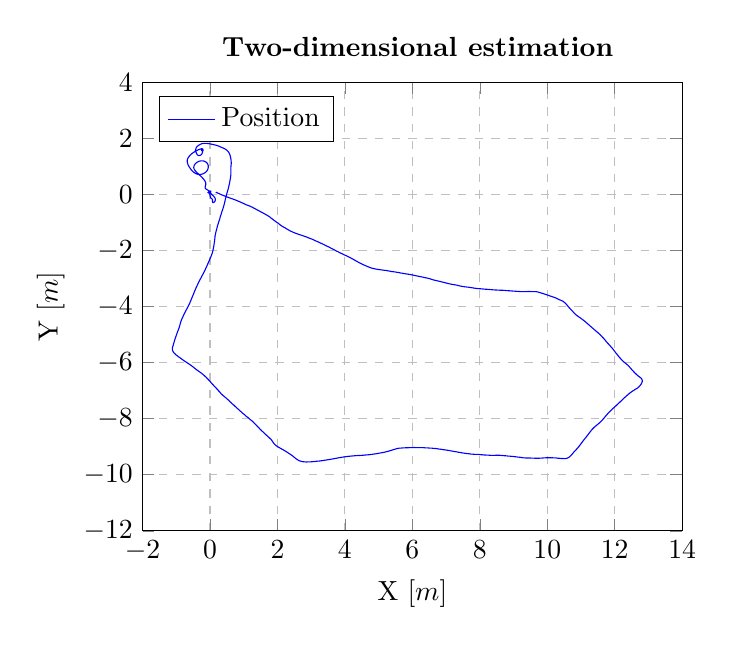
\begin{tikzpicture}
\begin{axis}[
    title={\textbf{ Two-dimensional estimation}},
    xlabel={X [$m$]},
    ylabel={Y [$m$]},
    xmin=-2, xmax=14,
    ymin=-12, ymax=4,
    xtick distance = 2,
    ytick distance = 2,
    % ytick={-80,-60,-40,-20,0,20,40,60,80,100},
    legend pos=north west,
    xmajorgrids=true,
    ymajorgrids=true,
    grid style=dashed,
]

\addplot[
    color=blue
    ]
    coordinates {(0.02268617,0.1165467)
(0.02266622,0.1165622)
(0.02265028,0.1165747)
(0.02263753,0.1165847)
(0.02262731,0.1165926)
(0.02261906,0.1165989)
(0.02261241,0.1166038)
(0.02260704,0.1166077)
(0.02260273,0.1166108)
(0.02259925,0.1166133)
(0.02259648,0.1166152)
(0.02259426,0.1166168)
(0.02259251,0.1166181)
(0.02259113,0.1166191)
(0.02259004,0.11662)
(0.02258919,0.1166207)
(0.02258851,0.1166213)
(0.02258797,0.1166217)
(0.02258754,0.1166221)
(0.02258719,0.1166224)
(0.02258692,0.1166227)
(0.02258671,0.1166229)
(0.02258654,0.116623)
(0.02258641,0.1166232)
(0.02243895,0.1167889)
(0.02221541,0.1170705)
(0.02207642,0.1172553)
(0.02196765,0.1174049)
(0.0218829,0.1175262)
(0.02181807,0.1176252)
(0.02176982,0.1177067)
(0.02173461,0.1177738)
(0.02170951,0.117829)
(0.02169229,0.1178743)
(0.02160412,0.1181563)
(0.02156155,0.1183214)
(0.02153693,0.1184556)
(0.02152326,0.1185638)
(0.02151341,0.1189022)
(0.02153966,0.1194397)
(0.02158829,0.1197933)
(0.0216654,0.1200682)
(0.0218604,0.1205145)
(0.02203903,0.1207989)
(0.02220953,0.1210066)
(0.02236636,0.1211536)
(0.02250557,0.1212546)
(0.02262371,0.1213251)
(0.02272149,0.1213756)
(0.02280147,0.1214125)
(0.02286816,0.1214351)
(0.02292223,0.121451)
(0.02296619,0.121461)
(0.02300169,0.1214674)
(0.02303039,0.1214703)
(0.02305344,0.1214715)
(0.02307189,0.1214724)
(0.0230866,0.1214737)
(0.02309833,0.1214752)
(0.02310775,0.121476)
(0.02311531,0.1214763)
(0.02312135,0.1214765)
(0.02312619,0.1214767)
(0.02313006,0.1214765)
(0.02313316,0.1214763)
(0.02313561,0.121476)
(0.02313757,0.1214757)
(0.02313915,0.1214755)
(0.0231404,0.1214753)
(0.02314139,0.1214751)
(0.02314217,0.1214749)
(0.02314279,0.1214747)
(0.02314327,0.1214745)
(0.02314364,0.1214743)
(0.02314393,0.1214741)
(0.02314414,0.121474)
(0.02314431,0.1214738)
(0.02314444,0.1214737)
(0.02314454,0.1214736)
(0.02314461,0.1214736)
(0.02314467,0.1214735)
(0.02314471,0.1214734)
(0.02314475,0.1214734)
(0.02314477,0.1214734)
(0.02314479,0.1214733)
(0.02314481,0.1214733)
(0.02314481,0.1214733)
(0.02314482,0.1214733)
(0.0232311,0.1212114)
(0.02327115,0.1210699)
(0.02334947,0.1207286)
(0.02338965,0.1205062)
(0.0234454,0.1200537)
(0.02348639,0.1193749)
(0.02348813,0.1183968)
(0.02340939,0.1171485)
(0.02329083,0.116264)
(0.02304482,0.1150793)
(0.02261048,0.1135167)
(0.02194307,0.1116062)
(0.02111448,0.1096627)
(0.02038808,0.1082198)
(0.01945169,0.106623)
(0.01824231,0.1048606)
(0.01681283,0.1030639)
(0.0151116,0.1012377)
(0.01370669,0.09993123)
(0.0120659,0.09860769)
(0.009919396,0.09708479)
(0.007474994,0.09555491)
(0.005559563,0.09449814)
(0.003986118,0.09373191)
(0.002698981,0.09318102)
(0.001158522,0.09260756)
(-0.0005821338,0.09210099)
(-0.002814684,0.091555)
(-0.004465724,0.09120872)
(-0.00656251,0.09084869)
(-0.00883724,0.09053433)
(-0.01150723,0.09024973)
(-0.01351951,0.09012154)
(-0.01580924,0.0901195)
(-0.01756312,0.0902521)
(-0.01949003,0.09058493)
(-0.02155924,0.09112159)
(-0.02311317,0.0916585)
(-0.02492913,0.09238049)
(-0.02628422,0.09297726)
(-0.0273526,0.09348882)
(-0.02818081,0.09394932)
(-0.02881747,0.09436089)
(-0.02930501,0.09472162)
(-0.02967313,0.09503767)
(-0.02994862,0.09531111)
(-0.03041599,0.09584413)
(-0.0310235,0.09664479)
(-0.03162341,0.09759294)
(-0.03202334,0.09832089)
(-0.03251345,0.09939626)
(-0.03305685,0.1007382)
(-0.03340076,0.1017367)
(-0.03365007,0.1025439)
(-0.03382952,0.1031955)
(-0.03396114,0.10372)
(-0.03406251,0.1041405)
(-0.03414018,0.1044777)
(-0.03425813,0.1050248)
(-0.03432374,0.10541)
(-0.03440318,0.1061356)
(-0.03442814,0.1070897)
(-0.03438316,0.1081489)
(-0.034293,0.1089337)
(-0.03417538,0.1095546)
(-0.03405364,0.1100452)
(-0.03391817,0.1104263)
(-0.03368807,0.1110085)
(-0.03350497,0.1114105)
(-0.03333749,0.1117217)
(-0.03293219,0.1123552)
(-0.0323602,0.1130462)
(-0.03191301,0.113509)
(-0.03119646,0.1141165)
(-0.03064919,0.1145076)
(-0.02990748,0.1149668)
(-0.02933232,0.1152578)
(-0.02886141,0.115468)
(-0.02810361,0.1157861)
(-0.02759128,0.116049)
(-0.02718354,0.1162634)
(-0.02648487,0.1165774)
(-0.02598156,0.1167477)
(-0.02557331,0.1168662)
(-0.02482042,0.1170662)
(-0.02430788,0.1171963)
(-0.02389703,0.1172972)
(-0.02356865,0.1173791)
(-0.02330534,0.1174422)
(-0.02271249,0.117609)
(-0.0223368,0.1177483)
(-0.02204015,0.1178697)
(-0.02180274,0.1179666)
(-0.02160494,0.118021)
(-0.02120449,0.1181024)
(-0.02093414,0.1181378)
(-0.02071684,0.1181567)
(-0.02054238,0.1181533)
(-0.0199965,0.1181141)
(-0.01910633,0.1180123)
(-0.01817335,0.1178828)
(-0.01749017,0.1177337)
(-0.01695023,0.1175874)
(-0.01652671,0.1174429)
(-0.0161914,0.1173174)
(-0.01592742,0.1172063)
(-0.01547893,0.1169907)
(-0.01518567,0.1168152)
(-0.01467361,0.1164251)
(-0.01392419,0.1157256)
(-0.01291348,0.1145881)
(-0.01229284,0.113751)
(-0.01184639,0.1130469)
(-0.01152322,0.1124635)
(-0.01110397,0.1116426)
(-0.01082369,0.1110346)
(-0.0104817,0.1101954)
(-0.01009199,0.1090426)
(-0.009620901,0.1071856)
(-0.009209179,0.1049217)
(-0.008935454,0.1023444)
(-0.008865163,0.1004085)
(-0.008916196,0.09885965)
(-0.009063993,0.09712352)
(-0.009289657,0.09505715)
(-0.009487518,0.09351366)
(-0.009770843,0.09171524)
(-0.01016679,0.08977438)
(-0.01082624,0.08729574)
(-0.01172572,0.08460272)
(-0.01294068,0.08158237)
(-0.01397503,0.07936219)
(-0.01489702,0.07763323)
(-0.01569629,0.07628477)
(-0.01638178,0.07523466)
(-0.0169654,0.07441866)
(-0.01745846,0.0737854)
(-0.01812254,0.07298336)
(-0.01902892,0.07196646)
(-0.02023647,0.07073322)
(-0.02205665,0.06905151)
(-0.02342764,0.06798374)
(-0.02500959,0.06688254)
(-0.02677365,0.06576198)
(-0.02897586,0.06445718)
(-0.03064854,0.06355088)
(-0.03283156,0.06248108)
(-0.03526314,0.06138975)
(-0.03786093,0.06046796)
(-0.03993205,0.05991222)
(-0.04162046,0.05960852)
(-0.04298592,0.05947065)
(-0.04408341,0.05943976)
(-0.04546241,0.05950097)
(-0.04709745,0.0596714)
(-0.04829982,0.05987649)
(-0.04925186,0.06009045)
(-0.05000095,0.06031012)
(-0.05096508,0.06066829)
(-0.05165212,0.06098547)
(-0.05218095,0.06128011)
(-0.05289555,0.06174945)
(-0.05339366,0.06211424)
(-0.05377834,0.06242406)
(-0.05435316,0.06293294)
(-0.05510436,0.06365346)
(-0.05591193,0.06456233)
(-0.05676162,0.06567847)
(-0.05734988,0.06654339)
(-0.05780243,0.06724726)
(-0.05815145,0.06781852)
(-0.0584211,0.06828123)
(-0.05863328,0.06865345)
(-0.05880087,0.06895244)
(-0.0590584,0.06943696)
(-0.05938634,0.07011616)
(-0.05959082,0.07060542)
(-0.05973044,0.071006)
(-0.0598264,0.07133152)
(-0.05988907,0.07159569)
(-0.05993867,0.07180715)
(-0.06002735,0.07225385)
(-0.06009877,0.07294559)
(-0.06011222,0.07341656)
(-0.06010283,0.07379336)
(-0.06008031,0.07409406)
(-0.06000023,0.07460573)
(-0.05975539,0.07545736)
(-0.0592946,0.07651741)
(-0.05866688,0.07760655)
(-0.05810782,0.07836428)
(-0.05717196,0.07937752)
(-0.05601954,0.08035229)
(-0.05461436,0.08125813)
(-0.0534667,0.08180111)
(-0.0524965,0.08210174)
(-0.05169287,0.08222185)
(-0.05104282,0.08222256)
(-0.0502152,0.08201567)
(-0.04928271,0.08163318)
(-0.04824851,0.08104323)
(-0.04753543,0.08052076)
(-0.04672284,0.07979112)
(-0.04615627,0.07920084)
(-0.04573205,0.07870236)
(-0.04541102,0.07828868)
(-0.04516536,0.07794936)
(-0.04497562,0.07767311)
(-0.04482327,0.07745251)
(-0.04469981,0.07727713)
(-0.0445999,0.07713762)
(-0.04451935,0.07702647)
(-0.04445457,0.0769378)
(-0.04440425,0.07686579)
(-0.04436491,0.07680755)
(-0.04433368,0.07676079)
(-0.04411823,0.07644344)
(-0.04399337,0.07626285)
(-0.043293,0.07526808)
(-0.04236738,0.07395243)
(-0.04089942,0.07161857)
(-0.03942793,0.06902242)
(-0.03806574,0.06631717)
(-0.03708229,0.06418306)
(-0.03631928,0.06246503)
(-0.0357188,0.06108624)
(-0.03520012,0.0600007)
(-0.03446144,0.05864275)
(-0.03336863,0.05693247)
(-0.03256716,0.05570709)
(-0.03104833,0.05334509)
(-0.02924969,0.05030831)
(-0.02770954,0.04730266)
(-0.02657408,0.04492101)
(-0.02571621,0.04299242)
(-0.02506025,0.04143641)
(-0.02426534,0.03968985)
(-0.02329643,0.03785944)
(-0.02205467,0.03602635)
(-0.02067052,0.03415158)
(-0.01891731,0.03177953)
(-0.01672974,0.02847457)
(-0.01467021,0.02477806)
(-0.01286013,0.02096158)
(-0.01113797,0.0167207)
(-0.00997841,0.01336749)
(-0.008915835,0.009721052)
(-0.007850659,0.005773252)
(-0.006670957,0.001633685)
(-0.005331248,-0.002663635)
(-0.003885704,-0.007222232)
(-0.002228644,-0.01239125)
(-0.0004526172,-0.01852028)
(0.001116815,-0.02460872)
(0.00225571,-0.02942317)
(0.002945247,-0.03332049)
(0.003442708,-0.03644744)
(0.004064688,-0.03976883)
(0.00488351,-0.04321993)
(0.005911067,-0.04695384)
(0.006774922,-0.0498164)
(0.007742461,-0.05319745)
(0.008858858,-0.05751469)
(0.009798635,-0.06184347)
(0.01042461,-0.06523847)
(0.01081585,-0.06797238)
(0.01108359,-0.07016552)
(0.01131145,-0.07191831)
(0.01166129,-0.0738751)
(0.01213486,-0.07609683)
(0.01269902,-0.07849389)
(0.01358713,-0.08152143)
(0.0145355,-0.08478251)
(0.01543118,-0.08819143)
(0.01606041,-0.09085866)
(0.01648763,-0.09300899)
(0.01675542,-0.09474231)
(0.01699372,-0.09612502)
(0.0173203,-0.09771654)
(0.01784745,-0.09945731)
(0.01857876,-0.1012887)
(0.01917571,-0.102679)
(0.02010605,-0.104842)
(0.02113697,-0.1075043)
(0.02179283,-0.1094737)
(0.02221086,-0.1110808)
(0.0224755,-0.1123826)
(0.02265127,-0.1134308)
(0.02278988,-0.1142696)
(0.02300328,-0.1153228)
(0.02328371,-0.1164843)
(0.02354075,-0.1173508)
(0.02423001,-0.1195208)
(0.02518711,-0.1222357)
(0.02600327,-0.1240839)
(0.02670943,-0.1255378)
(0.02722334,-0.1267243)
(0.02787308,-0.1281003)
(0.02847406,-0.1290883)
(0.02940574,-0.1303084)
(0.03066506,-0.1316584)
(0.03206151,-0.132936)
(0.03431726,-0.1349136)
(0.03681013,-0.1371369)
(0.03861195,-0.1388371)
(0.04000799,-0.1402438)
(0.0410718,-0.1414194)
(0.04191045,-0.142371)
(0.04261326,-0.1431029)
(0.04362516,-0.1439179)
(0.04444406,-0.1444256)
(0.04512959,-0.1447781)
(0.04623119,-0.1453481)
(0.04760445,-0.1460845)
(0.04904986,-0.146946)
(0.05050821,-0.1479769)
(0.05204279,-0.149185)
(0.05320228,-0.1501371)
(0.05413832,-0.1508884)
(0.05489616,-0.151478)
(0.05598413,-0.1523072)
(0.05674292,-0.1529362)
(0.05834662,-0.1543385)
(0.06030101,-0.1562656)
(0.06218364,-0.15852)
(0.06345249,-0.1603292)
(0.06484547,-0.1627182)
(0.06606345,-0.1652803)
(0.06714098,-0.1680956)
(0.06786633,-0.1703219)
(0.06840554,-0.1721158)
(0.06914618,-0.1746877)
(0.07012949,-0.177974)
(0.07151255,-0.1828852)
(0.07262936,-0.1880505)
(0.07345154,-0.193532)
(0.07391582,-0.1991428)
(0.07396681,-0.2035751)
(0.07386261,-0.2071196)
(0.07373418,-0.2099535)
(0.07361239,-0.2130201)
(0.0735405,-0.2162779)
(0.07357589,-0.2196411)
(0.07356681,-0.2240722)
(0.07348912,-0.2293417)
(0.07329449,-0.2347494)
(0.07305793,-0.2389259)
(0.0727708,-0.2422601)
(0.0725167,-0.2449253)
(0.07236738,-0.2470619)
(0.07224745,-0.2494055)
(0.07221795,-0.2520922)
(0.07242381,-0.2549422)
(0.07281672,-0.257111)
(0.07333903,-0.2595502)
(0.07397026,-0.2627266)
(0.07437755,-0.2650578)
(0.07470722,-0.2669222)
(0.07504228,-0.2683993)
(0.07531033,-0.269581)
(0.07568936,-0.2709508)
(0.07625759,-0.2726637)
(0.07709631,-0.274492)
(0.07833701,-0.2764208)
(0.08000182,-0.278396)
(0.08143514,-0.2797236)
(0.08359974,-0.2813639)
(0.08597967,-0.2827368)
(0.08795286,-0.2835169)
(0.09026632,-0.2840778)
(0.09289145,-0.2841922)
(0.0948985,-0.2840353)
(0.09708603,-0.283666)
(0.09874365,-0.2832069)
(0.1000408,-0.2827477)
(0.1016832,-0.2821133)
(0.1033905,-0.2813866)
(0.1059891,-0.2801873)
(0.1096588,-0.2784147)
(0.1130347,-0.2765771)
(0.115632,-0.2750819)
(0.1176972,-0.2738642)
(0.1200531,-0.2723784)
(0.1217526,-0.271103)
(0.1243118,-0.26894)
(0.1273875,-0.2660882)
(0.1307253,-0.2626011)
(0.1336715,-0.2589255)
(0.1366459,-0.2547291)
(0.1396502,-0.2501544)
(0.1417921,-0.2464892)
(0.1440299,-0.242462)
(0.1465604,-0.2376139)
(0.1488633,-0.2324152)
(0.1508639,-0.2269929)
(0.1527052,-0.2210479)
(0.154397,-0.2149542)
(0.1555321,-0.2101003)
(0.1565562,-0.2044465)
(0.1572221,-0.198666)
(0.1576685,-0.1918882)
(0.1577787,-0.1842824)
(0.1574756,-0.1764364)
(0.1568968,-0.1703522)
(0.1560864,-0.1636268)
(0.1550448,-0.1564741)
(0.1537615,-0.1489012)
(0.1520957,-0.1407055)
(0.1500249,-0.1323101)
(0.1470283,-0.1224948)
(0.143154,-0.1118867)
(0.1396521,-0.1040332)
(0.1355703,-0.09616678)
(0.132022,-0.09010998)
(0.1280024,-0.08400773)
(0.1235727,-0.07777922)
(0.1188276,-0.07133638)
(0.1138495,-0.06483921)
(0.1084715,-0.05818257)
(0.1026232,-0.05129461)
(0.0960343,-0.04403957)
(0.08845067,-0.03608695)
(0.0805016,-0.02811064)
(0.0741639,-0.02200315)
(0.06756259,-0.01562287)
(0.06253009,-0.01041312)
(0.05874857,-0.006022274)
(0.05506055,-0.001149721)
(0.05219708,0.002708143)
(0.04922853,0.006778016)
(0.04570935,0.01175302)
(0.04176454,0.01742323)
(0.03798759,0.02301681)
(0.03409745,0.02908108)
(0.03035943,0.03535679)
(0.02664252,0.04197747)
(0.02300559,0.04895766)
(0.01942857,0.05613106)
(0.01582413,0.06367177)
(0.01151434,0.07216645)
(0.008046366,0.07855633)
(0.004300611,0.08513815)
(0.0004815022,0.09181972)
(-0.002607605,0.09707636)
(-0.005988722,0.102492)
(-0.009827293,0.1081329)
(-0.01404084,0.1136804)
(-0.0175587,0.1178916)
(-0.0216317,0.1223855)
(-0.02640624,0.12733)
(-0.03156392,0.1322931)
(-0.03683462,0.1371455)
(-0.04244512,0.1420663)
(-0.04826816,0.1469683)
(-0.05463135,0.1521892)
(-0.0614254,0.1575771)
(-0.06875453,0.1631692)
(-0.07629499,0.1685728)
(-0.08456508,0.174175)
(-0.09320354,0.179816)
(-0.09997761,0.1842451)
(-0.1052986,0.1879343)
(-0.1106774,0.1922336)
(-0.114742,0.1957874)
(-0.1189866,0.1995942)
(-0.123649,0.2039178)
(-0.127128,0.2073467)
(-0.1310474,0.2115885)
(-0.1347992,0.2163653)
(-0.1378044,0.2217812)
(-0.1403478,0.2280566)
(-0.1421806,0.2349689)
(-0.1432348,0.2424931)
(-0.1433568,0.250077)
(-0.1429716,0.2560783)
(-0.1424959,0.2631664)
(-0.1421766,0.2703749)
(-0.1419092,0.2776508)
(-0.1411829,0.2853205)
(-0.1397339,0.293425)
(-0.1380158,0.2995912)
(-0.1357879,0.307375)
(-0.13429,0.3132109)
(-0.1325039,0.3200322)
(-0.1312146,0.3252424)
(-0.1294861,0.332809)
(-0.12816,0.3399376)
(-0.12681,0.347623)
(-0.1256668,0.3556078)
(-0.1247422,0.3651801)
(-0.1246054,0.3747503)
(-0.1248985,0.3854027)
(-0.1255432,0.3960527)
(-0.1269742,0.4078173)
(-0.1293344,0.420185)
(-0.1325017,0.4322179)
(-0.1361662,0.4449008)
(-0.1393868,0.4547234)
(-0.1436068,0.4658209)
(-0.1486172,0.4771688)
(-0.1540798,0.4882728)
(-0.1599695,0.5001571)
(-0.1661023,0.5118141)
(-0.173307,0.5243315)
(-0.1812342,0.5367848)
(-0.1898627,0.5493446)
(-0.1988874,0.5621613)
(-0.2063112,0.5720416)
(-0.2146879,0.5827964)
(-0.2233876,0.5936294)
(-0.23224,0.6045945)
(-0.2413871,0.6162469)
(-0.248469,0.6254603)
(-0.2563187,0.6354452)
(-0.2646997,0.6454673)
(-0.2734389,0.6555328)
(-0.2826039,0.6662363)
(-0.2898743,0.6745242)
(-0.2981632,0.6836611)
(-0.3064675,0.6925925)
(-0.3150282,0.702202)
(-0.3232811,0.7124001)
(-0.3318237,0.7228589)
(-0.3411907,0.734094)
(-0.3486783,0.7426282)
(-0.3569284,0.7521439)
(-0.3631098,0.7596768)
(-0.3697464,0.7675829)
(-0.3771552,0.7761204)
(-0.3846447,0.7844679)
(-0.3927666,0.7937642)
(-0.4004558,0.8033682)
(-0.4085533,0.813583)
(-0.4171259,0.8243171)
(-0.4238741,0.8326549)
(-0.4309593,0.8419604)
(-0.4377475,0.8520457)
(-0.4443508,0.8623571)
(-0.4514374,0.8733994)
(-0.4568476,0.8820837)
(-0.4623483,0.8916268)
(-0.4665637,0.9022514)
(-0.4705317,0.9131188)
(-0.4745852,0.9249467)
(-0.4779396,0.9369566)
(-0.4802769,0.9502078)
(-0.4813461,0.9644258)
(-0.4806261,0.9788343)
(-0.4789723,0.9937078)
(-0.476502,1.008564)
(-0.4731101,1.023794)
(-0.4684973,1.039773)
(-0.4618876,1.054872)
(-0.4540381,1.069563)
(-0.4455385,1.084504)
(-0.4356524,1.099043)
(-0.4244168,1.113556)
(-0.4142979,1.123836)
(-0.4032192,1.134458)
(-0.3944343,1.142679)
(-0.384867,1.150655)
(-0.3745846,1.157981)
(-0.3635827,1.165103)
(-0.3516303,1.172846)
(-0.3422979,1.178742)
(-0.331941,1.184256)
(-0.3209037,1.189044)
(-0.3094797,1.192934)
(-0.2970468,1.196596)
(-0.2842453,1.199554)
(-0.2702766,1.202209)
(-0.2558171,1.204017)
(-0.2410203,1.204353)
(-0.2254749,1.20387)
(-0.2133511,1.202521)
(-0.2004251,1.200419)
(-0.1876967,1.197298)
(-0.1748475,1.19268)
(-0.1611134,1.186867)
(-0.1480028,1.179804)
(-0.1347311,1.17162)
(-0.1221387,1.162302)
(-0.1096938,1.150926)
(-0.09794932,1.137892)
(-0.08731967,1.123905)
(-0.07984967,1.112126)
(-0.0731666,1.099483)
(-0.06676148,1.085072)
(-0.06149846,1.070261)
(-0.05712733,1.054698)
(-0.05444753,1.042212)
(-0.05224472,1.028761)
(-0.0506363,1.013535)
(-0.05029178,0.9981779)
(-0.05103335,0.9824588)
(-0.052631,0.9665118)
(-0.05513954,0.9502443)
(-0.05844701,0.932698)
(-0.06275362,0.9150981)
(-0.06868754,0.8972724)
(-0.07406366,0.8835037)
(-0.08034984,0.8691169)
(-0.08778131,0.854141)
(-0.09431779,0.842879)
(-0.1019598,0.8313168)
(-0.1084517,0.8226055)
(-0.1161737,0.8131706)
(-0.1247687,0.8036791)
(-0.1342032,0.7943017)
(-0.1440235,0.7854138)
(-0.1545838,0.7766356)
(-0.1664023,0.7675344)
(-0.17849,0.7592385)
(-0.1917321,0.7509889)
(-0.2024385,0.7451139)
(-0.2142104,0.7393971)
(-0.2272458,0.7337573)
(-0.2376006,0.7300836)
(-0.2494986,0.7266002)
(-0.2614207,0.7239361)
(-0.2744714,0.7216987)
(-0.2882324,0.7199703)
(-0.3022718,0.7190154)
(-0.3175337,0.7186337)
(-0.3293714,0.7191044)
(-0.3420284,0.7202596)
(-0.3553388,0.7222034)
(-0.3655599,0.7245487)
(-0.3764891,0.7279379)
(-0.3872921,0.7321251)
(-0.3985583,0.7371654)
(-0.4102323,0.743114)
(-0.4214669,0.7497175)
(-0.4331002,0.7573533)
(-0.4447455,0.765767)
(-0.4562156,0.7746027)
(-0.4681591,0.7843523)
(-0.4797082,0.7944438)
(-0.4913141,0.8056447)
(-0.5026842,0.8177046)
(-0.5112334,0.8275807)
(-0.5206254,0.8386222)
(-0.5300124,0.8499475)
(-0.5398156,0.8623631)
(-0.5491088,0.8753715)
(-0.5579509,0.8886771)
(-0.5672975,0.9030632)
(-0.5766081,0.9174669)
(-0.5860959,0.9327383)
(-0.5950604,0.9488267)
(-0.6035585,0.9650967)
(-0.6127207,0.9822916)
(-0.6219265,1.00019)
(-0.6308604,1.018578)
(-0.6398025,1.038211)
(-0.647531,1.058512)
(-0.6547453,1.0801)
(-0.6612825,1.102184)
(-0.6669584,1.125129)
(-0.6719765,1.149161)
(-0.6742205,1.168352)
(-0.6757237,1.189055)
(-0.6759634,1.210421)
(-0.6734216,1.231776)
(-0.6692257,1.253988)
(-0.6625977,1.275683)
(-0.6544169,1.297591)
(-0.6450194,1.319507)
(-0.6333345,1.340893)
(-0.6200032,1.362154)
(-0.6050231,1.382195)
(-0.5886185,1.402598)
(-0.5721178,1.423093)
(-0.5543432,1.443484)
(-0.5351974,1.46332)
(-0.5189262,1.477881)
(-0.5016305,1.492741)
(-0.4839105,1.507584)
(-0.4650411,1.522847)
(-0.4449034,1.537994)
(-0.423901,1.551473)
(-0.4019969,1.565258)
(-0.3849658,1.576557)
(-0.3668214,1.58765)
(-0.3478725,1.59735)
(-0.3322632,1.603958)
(-0.3162183,1.610527)
(-0.3034877,1.615767)
(-0.290668,1.621315)
(-0.2805258,1.625878)
(-0.2723636,1.629419)
(-0.2657875,1.632142)
(-0.2603902,1.633956)
(-0.2546668,1.635583)
(-0.2500659,1.636502)
(-0.2463428,1.636977)
(-0.2433464,1.637173)
(-0.2409444,1.637198)
(-0.2390246,1.637111)
(-0.2374903,1.637014)
(-0.2362698,1.636862)
(-0.2353086,1.636652)
(-0.2345575,1.636416)
(-0.2339666,1.636199)
(-0.2335007,1.636007)
(-0.2331364,1.635835)
(-0.2328598,1.635669)
(-0.2326434,1.635529)
(-0.2324788,1.635404)
(-0.2323443,1.635308)
(-0.2322382,1.63523)
(-0.2321558,1.635164)
(-0.2320913,1.635109)
(-0.2320413,1.635064)
(-0.2320025,1.635026)
(-0.2319723,1.634995)
(-0.2319485,1.63497)
(-0.2319298,1.634949)
(-0.2319149,1.634933)
(-0.2319032,1.63492)
(-0.2318942,1.634909)
(-0.2318873,1.6349)
(-0.2318818,1.634892)
(-0.2318774,1.634887)
(-0.2318739,1.634882)
(-0.2318711,1.634878)
(-0.2318689,1.634875)
(-0.2318671,1.634873)
(-0.2318657,1.634871)
(-0.2318646,1.634869)
(-0.2318638,1.634868)
(-0.2318631,1.634867)
(-0.2318625,1.634866)
(-0.231862,1.634866)
(-0.2318617,1.634865)
(-0.2318614,1.634865)
(-0.2318611,1.634865)
(-0.2316884,1.634635)
(-0.2315946,1.634514)
(-0.2315211,1.634416)
(-0.2314626,1.634337)
(-0.231417,1.634273)
(-0.2313801,1.634222)
(-0.23135,1.634182)
(-0.2313255,1.63415)
(-0.2311245,1.633899)
(-0.2310112,1.633756)
(-0.2307594,1.633449)
(-0.2300202,1.632595)
(-0.2290035,1.631477)
(-0.227677,1.630141)
(-0.226056,1.628663)
(-0.2248423,1.62759)
(-0.2233323,1.626273)
(-0.2222081,1.625279)
(-0.2209272,1.624152)
(-0.2199361,1.623295)
(-0.2191411,1.622613)
(-0.2184917,1.622082)
(-0.2179701,1.621661)
(-0.2172543,1.621073)
(-0.2167315,1.62065)
(-0.2163103,1.620315)
(-0.2159749,1.620045)
(-0.2157084,1.619827)
(-0.2154975,1.61965)
(-0.2153317,1.619504)
(-0.2152,1.619387)
(-0.2146774,1.618907)
(-0.2143703,1.618613)
(-0.2139351,1.618129)
(-0.2136534,1.617765)
(-0.2126695,1.616446)
(-0.2117868,1.61515)
(-0.2111347,1.61418)
(-0.2106127,1.613403)
(-0.2101938,1.612783)
(-0.2098622,1.612284)
(-0.2096108,1.611877)
(-0.2092156,1.611106)
(-0.2085244,1.609582)
(-0.2078743,1.607858)
(-0.2073121,1.606025)
(-0.2069614,1.604596)
(-0.2065098,1.602475)
(-0.2061511,1.600273)
(-0.2059344,1.59858)
(-0.2056986,1.596652)
(-0.2054721,1.595179)
(-0.2051453,1.593285)
(-0.2048184,1.591201)
(-0.2045597,1.589623)
(-0.2043529,1.58836)
(-0.2041875,1.58735)
(-0.2040801,1.586539)
(-0.2040263,1.585886)
(-0.2040085,1.585002)
(-0.204027,1.584356)
(-0.2040737,1.583841)
(-0.204352,1.582114)
(-0.2048822,1.579758)
(-0.2056276,1.577221)
(-0.2065815,1.574693)
(-0.2074779,1.5728)
(-0.2087531,1.57068)
(-0.2103256,1.568581)
(-0.2121858,1.566574)
(-0.2138099,1.565189)
(-0.2158651,1.563822)
(-0.2183734,1.562564)
(-0.2213689,1.561536)
(-0.224608,1.560913)
(-0.2281885,1.560715)
(-0.2309418,1.560971)
(-0.2339581,1.561728)
(-0.2371793,1.563043)
(-0.2402245,1.564849)
(-0.2424042,1.566563)
(-0.2445971,1.568784)
(-0.2465883,1.571341)
(-0.2484496,1.574299)
(-0.2501309,1.577538)
(-0.2513174,1.580128)
(-0.2521838,1.582236)
(-0.2528272,1.583942)
(-0.2535465,1.585911)
(-0.2540691,1.587428)
(-0.2545781,1.589205)
(-0.2550433,1.591366)
(-0.2554511,1.593772)
(-0.2557092,1.596284)
(-0.255774,1.598248)
(-0.2557385,1.599819)
(-0.2556406,1.601849)
(-0.2554821,1.603344)
(-0.2552066,1.605145)
(-0.2547942,1.607082)
(-0.2541556,1.609373)
(-0.2533257,1.611704)
(-0.2525723,1.61346)
(-0.2519811,1.614869)
(-0.2515187,1.616001)
(-0.2509593,1.617345)
(-0.2501949,1.618805)
(-0.2492469,1.620439)
(-0.2484409,1.621611)
(-0.2477382,1.622506)
(-0.2466818,1.623653)
(-0.2454654,1.62484)
(-0.2440836,1.626046)
(-0.2429553,1.626886)
(-0.2414173,1.627875)
(-0.2402075,1.628476)
(-0.2392175,1.628908)
(-0.2379293,1.629448)
(-0.236965,1.629819)
(-0.2357435,1.63025)
(-0.2348066,1.630488)
(-0.2340414,1.630599)
(-0.2330273,1.630688)
(-0.2322782,1.630689)
(-0.2316832,1.630618)
(-0.2312133,1.630523)
(-0.2305497,1.630338)
(-0.230079,1.630184)
(-0.2286311,1.62964)
(-0.2272073,1.628897)
(-0.2258143,1.627987)
(-0.2243871,1.626772)
(-0.2228909,1.625195)
(-0.2213298,1.623086)
(-0.2198341,1.620533)
(-0.2185059,1.617504)
(-0.2174197,1.614045)
(-0.2165731,1.609904)
(-0.2160617,1.605503)
(-0.2156349,1.600762)
(-0.2151018,1.595981)
(-0.2145852,1.590923)
(-0.2141365,1.585038)
(-0.2139671,1.578388)
(-0.2141906,1.57117)
(-0.2144893,1.563731)
(-0.2149337,1.557933)
(-0.2155025,1.553317)
(-0.2161481,1.549652)
(-0.2168819,1.545654)
(-0.2174755,1.54255)
(-0.2179774,1.539185)
(-0.2182303,1.53654)
(-0.2184794,1.534428)
(-0.2187823,1.531953)
(-0.2190412,1.530073)
(-0.2192769,1.528574)
(-0.2194875,1.527378)
(-0.2196537,1.526421)
(-0.2197763,1.525654)
(-0.2198711,1.52504)
(-0.2199992,1.52415)
(-0.2201657,1.522836)
(-0.2202847,1.521923)
(-0.2205403,1.520398)
(-0.2209143,1.518681)
(-0.2213871,1.516909)
(-0.2218101,1.515565)
(-0.2221848,1.514501)
(-0.2226312,1.513229)
(-0.2230846,1.511798)
(-0.2235394,1.509988)
(-0.2239952,1.507641)
(-0.2244409,1.504944)
(-0.2251806,1.50109)
(-0.226223,1.496564)
(-0.2275115,1.491885)
(-0.2286807,1.488351)
(-0.2301017,1.484575)
(-0.2316806,1.480531)
(-0.2334153,1.476114)
(-0.2350913,1.471531)
(-0.2363023,1.467909)
(-0.2380698,1.462948)
(-0.240144,1.457611)
(-0.2424026,1.452417)
(-0.2443462,1.448399)
(-0.2460329,1.445251)
(-0.247469,1.442782)
(-0.2486744,1.44084)
(-0.2500513,1.438659)
(-0.2517169,1.436095)
(-0.2534959,1.433419)
(-0.2562751,1.429432)
(-0.2594842,1.425035)
(-0.2627636,1.420807)
(-0.2655094,1.417628)
(-0.2678454,1.415212)
(-0.2704738,1.412757)
(-0.2733544,1.410281)
(-0.2767281,1.407583)
(-0.2805616,1.404762)
(-0.2835917,1.402752)
(-0.2880994,1.400069)
(-0.293221,1.397403)
(-0.2988366,1.395177)
(-0.3032954,1.3938)
(-0.308341,1.392671)
(-0.3123126,1.392179)
(-0.316547,1.391956)
(-0.3198755,1.391982)
(-0.3235752,1.392229)
(-0.3280445,1.39279)
(-0.3324684,1.39378)
(-0.3377536,1.395339)
(-0.3432781,1.397179)
(-0.3474643,1.398769)
(-0.3517929,1.400792)
(-0.356248,1.403495)
(-0.3604805,1.407017)
(-0.3645099,1.411223)
(-0.3682683,1.415826)
(-0.3722819,1.421126)
(-0.376656,1.427304)
(-0.3807196,1.433573)
(-0.3848863,1.440271)
(-0.3882302,1.44546)
(-0.3909794,1.449562)
(-0.393088,1.452903)
(-0.3949436,1.45676)
(-0.3964561,1.460962)
(-0.3978337,1.46532)
(-0.3993136,1.469843)
(-0.4009183,1.47451)
(-0.4026532,1.479671)
(-0.4042519,1.484946)
(-0.4061614,1.491231)
(-0.4083938,1.498105)
(-0.4102419,1.50329)
(-0.411882,1.507377)
(-0.4132284,1.510633)
(-0.4145639,1.514304)
(-0.4158788,1.51813)
(-0.4172584,1.522244)
(-0.4186484,1.526666)
(-0.4200068,1.531445)
(-0.4215847,1.537084)
(-0.4232936,1.542967)
(-0.424683,1.547495)
(-0.4255877,1.551174)
(-0.42629,1.555097)
(-0.4269174,1.559302)
(-0.427563,1.563738)
(-0.428348,1.568578)
(-0.4291532,1.573793)
(-0.4295837,1.577845)
(-0.4299024,1.58231)
(-0.4298563,1.585784)
(-0.429343,1.589526)
(-0.4283409,1.593357)
(-0.4269449,1.597255)
(-0.425483,1.601348)
(-0.4241306,1.605755)
(-0.4231836,1.609219)
(-0.4222499,1.613206)
(-0.42126,1.617795)
(-0.4202316,1.622702)
(-0.4193996,1.626469)
(-0.4187932,1.629495)
(-0.4181682,1.632832)
(-0.4177752,1.635436)
(-0.4175149,1.637526)
(-0.4173227,1.639814)
(-0.4171847,1.641595)
(-0.4169869,1.643797)
(-0.4167122,1.64613)
(-0.4163417,1.647897)
(-0.415936,1.649282)
(-0.4155541,1.650372)
(-0.4150883,1.651705)
(-0.4146617,1.653226)
(-0.4142636,1.65502)
(-0.4140236,1.656377)
(-0.4137023,1.658226)
(-0.4132675,1.660366)
(-0.4128111,1.661922)
(-0.4121435,1.663669)
(-0.4115423,1.664966)
(-0.4108499,1.666453)
(-0.4100606,1.668176)
(-0.4092618,1.669992)
(-0.408478,1.672063)
(-0.4079068,1.673656)
(-0.4072476,1.675595)
(-0.4063676,1.677984)
(-0.4056063,1.679695)
(-0.4045857,1.681591)
(-0.4032199,1.683749)
(-0.4017082,1.685936)
(-0.4001804,1.688274)
(-0.3990686,1.690143)
(-0.3982232,1.691664)
(-0.3972147,1.693436)
(-0.3960335,1.695361)
(-0.3950586,1.696781)
(-0.3941639,1.697828)
(-0.3934404,1.69866)
(-0.3929132,1.699366)
(-0.3925297,1.699958)
(-0.3920461,1.700802)
(-0.3917164,1.701428)
(-0.3911865,1.702324)
(-0.3904412,1.70349)
(-0.3898556,1.704284)
(-0.3891065,1.705209)
(-0.3881976,1.706272)
(-0.3872165,1.707486)
(-0.3865137,1.708435)
(-0.3857528,1.709583)
(-0.3849094,1.710952)
(-0.3838326,1.712519)
(-0.3829562,1.713632)
(-0.3818855,1.714856)
(-0.380594,1.71616)
(-0.3790741,1.717706)
(-0.3774932,1.719415)
(-0.3763604,1.720791)
(-0.3754515,1.721889)
(-0.374179,1.723293)
(-0.3726442,1.724924)
(-0.3710763,1.726567)
(-0.3698126,1.727798)
(-0.3683692,1.729189)
(-0.3667662,1.7307)
(-0.3648498,1.732617)
(-0.3628119,1.734558)
(-0.3596962,1.737459)
(-0.355437,1.741249)
(-0.3523042,1.743797)
(-0.3482898,1.747082)
(-0.3444575,1.750474)
(-0.339436,1.754945)
(-0.3339296,1.759566)
(-0.3280341,1.76415)
(-0.321349,1.76924)
(-0.3140112,1.774691)
(-0.3054073,1.780877)
(-0.2987064,1.785228)
(-0.2911119,1.790132)
(-0.2832986,1.794987)
(-0.2739771,1.800581)
(-0.2666953,1.804364)
(-0.2581471,1.808673)
(-0.2495164,1.812217)
(-0.2395997,1.815822)
(-0.2289163,1.818812)
(-0.2177076,1.820807)
(-0.2054786,1.822853)
(-0.196015,1.824429)
(-0.1845734,1.826101)
(-0.1730343,1.826915)
(-0.1609453,1.827367)
(-0.1479103,1.827859)
(-0.1350019,1.828212)
(-0.1204028,1.828212)
(-0.1062499,1.826774)
(-0.09099453,1.82526)
(-0.07573998,1.824229)
(-0.0591209,1.822651)
(-0.04238124,1.819467)
(-0.02583695,1.814911)
(-0.008563442,1.810306)
(0.005276022,1.807746)
(0.02110646,1.80479)
(0.03679748,1.80062)
(0.05285787,1.795932)
(0.06979179,1.791586)
(0.08774084,1.788029)
(0.1059715,1.783585)
(0.1241404,1.77776)
(0.1431222,1.771894)
(0.1626104,1.766467)
(0.183921,1.760135)
(0.2044263,1.752009)
(0.2255279,1.743032)
(0.2470832,1.733982)
(0.2691618,1.724114)
(0.2914634,1.712742)
(0.3080608,1.70212)
(0.3258501,1.691518)
(0.3444551,1.682649)
(0.3645084,1.673285)
(0.3849287,1.662896)
(0.4002215,1.653442)
(0.4162099,1.643582)
(0.4290933,1.636273)
(0.4434828,1.627936)
(0.457916,1.618235)
(0.4683712,1.609618)
(0.4795428,1.600134)
(0.4883595,1.592863)
(0.4980685,1.584242)
(0.5076689,1.574256)
(0.5142799,1.565827)
(0.5214578,1.556285)
(0.5287621,1.546976)
(0.5369054,1.536317)
(0.544858,1.524568)
(0.5502765,1.515002)
(0.5561296,1.50435)
(0.5619821,1.493776)
(0.5684727,1.481354)
(0.5738583,1.468392)
(0.5783138,1.455058)
(0.5829169,1.440839)
(0.5876525,1.426653)
(0.5926221,1.410917)
(0.5967758,1.394589)
(0.599929,1.378082)
(0.6029479,1.360651)
(0.6068939,1.343542)
(0.6111247,1.325356)
(0.6146127,1.306477)
(0.6163752,1.291466)
(0.6181204,1.275541)
(0.6205386,1.259651)
(0.6231446,1.24281)
(0.6251083,1.225277)
(0.6258154,1.211437)
(0.6262603,1.196764)
(0.6272449,1.181886)
(0.6284528,1.166002)
(0.6293007,1.149443)
(0.6293659,1.133006)
(0.6289961,1.115841)
(0.6287422,1.098172)
(0.628012,1.079248)
(0.6265467,1.064578)
(0.6246989,1.048745)
(0.6233892,1.032986)
(0.6221559,1.015804)
(0.6208979,0.9984259)
(0.6195025,0.9805416)
(0.6187469,0.9618539)
(0.6185897,0.9424349)
(0.6184315,0.9221174)
(0.6182999,0.9019986)
(0.6181127,0.8803069)
(0.6187255,0.8634029)
(0.6194344,0.8447219)
(0.6194621,0.8302409)
(0.6193304,0.8143932)
(0.6195603,0.7982242)
(0.6199796,0.7810495)
(0.6201478,0.7630649)
(0.6195217,0.7450483)
(0.6186076,0.7258667)
(0.6181847,0.7108638)
(0.6175613,0.6942489)
(0.6161521,0.6778579)
(0.6141378,0.6605974)
(0.6120317,0.6428548)
(0.6101857,0.6244482)
(0.6079425,0.6050451)
(0.6050187,0.5859835)
(0.6016397,0.5656116)
(0.5994626,0.5496207)
(0.5971892,0.5317564)
(0.5952519,0.5179839)
(0.5929697,0.5028972)
(0.591113,0.4878483)
(0.5892437,0.4714098)
(0.5868435,0.4548759)
(0.5838083,0.4379739)
(0.5805537,0.4201737)
(0.5777207,0.4022699)
(0.5746116,0.3829161)
(0.5709544,0.3639879)
(0.5668664,0.3440942)
(0.5630781,0.3239202)
(0.5594438,0.3028666)
(0.5553677,0.2811071)
(0.5506292,0.2594513)
(0.5455949,0.2368334)
(0.5421673,0.2189247)
(0.5384264,0.1994136)
(0.5340618,0.1801573)
(0.5289012,0.1601101)
(0.5238486,0.1397489)
(0.5188743,0.118448)
(0.5136765,0.09644394)
(0.5075212,0.07464449)
(0.5018482,0.0520365)
(0.4967543,0.02885596)
(0.4914464,0.004619241)
(0.4854128,-0.01957844)
(0.4791447,-0.04503561)
(0.4740458,-0.0707508)
(0.4687776,-0.09770093)
(0.4632093,-0.1247953)
(0.4577073,-0.1530762)
(0.4530659,-0.1815785)
(0.4480591,-0.2112246)
(0.4422627,-0.2407475)
(0.4359979,-0.2713313)
(0.4300261,-0.3017492)
(0.424038,-0.3336932)
(0.4185629,-0.3586816)
(0.4124239,-0.3848947)
(0.4077087,-0.4055435)
(0.4027164,-0.428062)
(0.3973746,-0.4501919)
(0.3912618,-0.4736922)
(0.3851941,-0.4969719)
(0.3787215,-0.5219281)
(0.3718741,-0.5470796)
(0.3644823,-0.5722187)
(0.3565692,-0.5985546)
(0.3493989,-0.6250861)
(0.3423077,-0.652195)
(0.3350903,-0.6806458)
(0.3275935,-0.7089577)
(0.319664,-0.7376327)
(0.3115944,-0.7671295)
(0.3038926,-0.7975421)
(0.2972063,-0.8280965)
(0.2903886,-0.8596721)
(0.2829544,-0.8918129)
(0.2744051,-0.9236027)
(0.264929,-0.9560327)
(0.2550409,-0.9892585)
(0.24849,-1.015877)
(0.2418402,-1.043476)
(0.2351189,-1.071978)
(0.2292859,-1.094331)
(0.2228207,-1.117277)
(0.2163747,-1.141393)
(0.2114649,-1.165751)
(0.2069855,-1.190723)
(0.202235,-1.217022)
(0.1967016,-1.242841)
(0.1902672,-1.269006)
(0.1834667,-1.296173)
(0.1775748,-1.323569)
(0.1723492,-1.351836)
(0.1671898,-1.381605)
(0.1616873,-1.411004)
(0.1555985,-1.440764)
(0.1499345,-1.471507)
(0.1484665,-1.496187)
(0.1471739,-1.522419)
(0.1456151,-1.549367)
(0.143664,-1.57054)
(0.1410544,-1.592425)
(0.1383023,-1.615048)
(0.1367923,-1.632947)
(0.1351969,-1.652259)
(0.1333841,-1.672461)
(0.1313659,-1.688191)
(0.1288749,-1.704624)
(0.1262752,-1.722164)
(0.1249634,-1.735923)
(0.1236014,-1.750836)
(0.1219577,-1.766723)
(0.1202361,-1.779013)
(0.1180543,-1.79185)
(0.1157774,-1.805494)
(0.1142815,-1.819216)
(0.1128399,-1.833867)
(0.1111112,-1.849755)
(0.1092672,-1.861976)
(0.1068297,-1.874779)
(0.1041241,-1.888645)
(0.1020554,-1.902581)
(0.09996132,-1.917751)
(0.09766206,-1.934068)
(0.09550477,-1.946635)
(0.09281219,-1.959946)
(0.0898595,-1.9743)
(0.08775658,-1.988637)
(0.08528164,-2.004269)
(0.08237037,-2.02085)
(0.07963658,-2.033633)
(0.07635958,-2.047134)
(0.0728026,-2.061673)
(0.06934017,-2.07611)
(0.06549254,-2.091907)
(0.06118897,-2.107989)
(0.05624708,-2.123989)
(0.05068504,-2.140894)
(0.0450536,-2.158274)
(0.03957987,-2.17608)
(0.03367519,-2.195318)
(0.0270754,-2.214382)
(0.01993738,-2.233781)
(0.01241182,-2.254051)
(0.005480724,-2.27471)
(-0.001439832,-2.296497)
(-0.008849483,-2.319303)
(-0.01505578,-2.337021)
(-0.02196336,-2.355361)
(-0.0292644,-2.374483)
(-0.03613767,-2.393569)
(-0.04344925,-2.413875)
(-0.05125923,-2.43494)
(-0.05945406,-2.455906)
(-0.06780883,-2.477764)
(-0.07528245,-2.499772)
(-0.08316612,-2.522924)
(-0.09168884,-2.547158)
(-0.1010446,-2.57082)
(-0.1110356,-2.5953)
(-0.1209097,-2.620613)
(-0.1280792,-2.640823)
(-0.1359881,-2.662755)
(-0.1444604,-2.684614)
(-0.1534257,-2.706314)
(-0.1629157,-2.728674)
(-0.1720186,-2.751605)
(-0.1807168,-2.775147)
(-0.1900449,-2.79966)
(-0.2001595,-2.824057)
(-0.2112176,-2.848303)
(-0.2234859,-2.873111)
(-0.2353192,-2.898394)
(-0.2469944,-2.924422)
(-0.258817,-2.951728)
(-0.2709356,-2.978653)
(-0.2835578,-3.005995)
(-0.2964582,-3.034451)
(-0.3082717,-3.063141)
(-0.3201076,-3.092942)
(-0.3324734,-3.123491)
(-0.3427795,-3.147393)
(-0.3537661,-3.171917)
(-0.364686,-3.197402)
(-0.3721192,-3.217979)
(-0.379429,-3.239805)
(-0.3874036,-3.26223)
(-0.3959321,-3.284309)
(-0.40512,-3.307127)
(-0.4141402,-3.330532)
(-0.4223142,-3.354525)
(-0.4309928,-3.380023)
(-0.4401469,-3.405294)
(-0.4498659,-3.430855)
(-0.4598852,-3.457342)
(-0.4666072,-3.478645)
(-0.4731861,-3.500999)
(-0.4801424,-3.524401)
(-0.4862289,-3.542557)
(-0.4931672,-3.561697)
(-0.5002059,-3.581731)
(-0.505299,-3.597579)
(-0.510898,-3.614511)
(-0.5169624,-3.631643)
(-0.5234393,-3.64864)
(-0.5304232,-3.666728)
(-0.5368655,-3.685318)
(-0.5431883,-3.704727)
(-0.5498558,-3.725242)
(-0.555414,-3.74116)
(-0.5616966,-3.758032)
(-0.567292,-3.775402)
(-0.5729104,-3.793752)
(-0.578978,-3.812757)
(-0.5841809,-3.827522)
(-0.5901266,-3.843304)
(-0.596004,-3.859742)
(-0.6019931,-3.876503)
(-0.6084732,-3.89425)
(-0.6155004,-3.911786)
(-0.6232687,-3.929728)
(-0.6315645,-3.948614)
(-0.6376769,-3.963556)
(-0.6442047,-3.979609)
(-0.6510982,-3.995873)
(-0.6584194,-4.012044)
(-0.6663147,-4.029343)
(-0.6737867,-4.047046)
(-0.6812653,-4.06538)
(-0.689333,-4.084814)
(-0.695972,-4.099844)
(-0.703178,-4.115784)
(-0.7104456,-4.132466)
(-0.7175765,-4.149321)
(-0.7250715,-4.167493)
(-0.7327845,-4.185771)
(-0.7409443,-4.204331)
(-0.7496481,-4.224062)
(-0.7575965,-4.243802)
(-0.7656454,-4.264781)
(-0.7740083,-4.286367)
(-0.7808324,-4.303267)
(-0.7883347,-4.321334)
(-0.7956086,-4.339899)
(-0.8028896,-4.358982)
(-0.810534,-4.379154)
(-0.8167061,-4.39487)
(-0.823395,-4.411425)
(-0.8302402,-4.428916)
(-0.8348251,-4.442875)
(-0.8397114,-4.458108)
(-0.8448809,-4.47353)
(-0.8504859,-4.489099)
(-0.8566085,-4.505937)
(-0.8614046,-4.523133)
(-0.8657624,-4.541163)
(-0.870202,-4.559814)
(-0.8740915,-4.574401)
(-0.8784328,-4.590125)
(-0.8824863,-4.606648)
(-0.8856197,-4.623251)
(-0.8890464,-4.641013)
(-0.892988,-4.658731)
(-0.897589,-4.676874)
(-0.9025987,-4.696146)
(-0.9071496,-4.715281)
(-0.9119548,-4.735585)
(-0.917345,-4.756326)
(-0.9237825,-4.776618)
(-0.9307364,-4.79805)
(-0.9370998,-4.819583)
(-0.9435498,-4.842254)
(-0.9505285,-4.865429)
(-0.9564821,-4.883561)
(-0.9633085,-4.902571)
(-0.9700309,-4.922539)
(-0.9741501,-4.938542)
(-0.9786176,-4.955686)
(-0.9834597,-4.972946)
(-0.9888929,-4.990178)
(-0.9948655,-5.00871)
(-1.000291,-5.027539)
(-1.005697,-5.047438)
(-1.011519,-5.068427)
(-1.017706,-5.089009)
(-1.024334,-5.110245)
(-1.031014,-5.132487)
(-1.03548,-5.150176)
(-1.040136,-5.169367)
(-1.04515,-5.189057)
(-1.05052,-5.208639)
(-1.056414,-5.229354)
(-1.061646,-5.250461)
(-1.066329,-5.272319)
(-1.071214,-5.295276)
(-1.075399,-5.3132)
(-1.080144,-5.331875)
(-1.085166,-5.351558)
(-1.088725,-5.36705)
(-1.09266,-5.383871)
(-1.09702,-5.401191)
(-1.101732,-5.418261)
(-1.106864,-5.436069)
(-1.111082,-5.454829)
(-1.113008,-5.469824)
(-1.114524,-5.486107)
(-1.115414,-5.502525)
(-1.115377,-5.519425)
(-1.114374,-5.537175)
(-1.111452,-5.555297)
(-1.107366,-5.569141)
(-1.102197,-5.583955)
(-1.096616,-5.598859)
(-1.089969,-5.61352)
(-1.081805,-5.628429)
(-1.071856,-5.642963)
(-1.060217,-5.656298)
(-1.047633,-5.670209)
(-1.035381,-5.684327)
(-1.023764,-5.699346)
(-1.011371,-5.714964)
(-0.9973264,-5.729575)
(-0.9817306,-5.742914)
(-0.9651627,-5.757185)
(-0.9496508,-5.772552)
(-0.9344097,-5.78862)
(-0.9173923,-5.803603)
(-0.8989574,-5.817115)
(-0.8798802,-5.831865)
(-0.8623583,-5.848059)
(-0.8452533,-5.865022)
(-0.8270008,-5.882066)
(-0.8111052,-5.89373)
(-0.7941316,-5.90617)
(-0.7771407,-5.919822)
(-0.7648173,-5.931704)
(-0.7520504,-5.944041)
(-0.738096,-5.95588)
(-0.7261075,-5.963924)
(-0.7128783,-5.972947)
(-0.6999545,-5.983089)
(-0.6879197,-5.994183)
(-0.6752439,-6.00567)
(-0.6614421,-6.01619)
(-0.6466724,-6.026435)
(-0.6311696,-6.037696)
(-0.6167765,-6.050214)
(-0.6024254,-6.063588)
(-0.5869937,-6.077269)
(-0.5737982,-6.086615)
(-0.5594864,-6.096988)
(-0.5457093,-6.108666)
(-0.5358519,-6.118904)
(-0.5257231,-6.129847)
(-0.5147293,-6.140979)
(-0.5051484,-6.148627)
(-0.4945281,-6.157292)
(-0.4845766,-6.166722)
(-0.4751629,-6.176995)
(-0.4652609,-6.18808)
(-0.4543056,-6.198572)
(-0.4423459,-6.209006)
(-0.4295148,-6.220634)
(-0.4178913,-6.233055)
(-0.4059282,-6.24581)
(-0.392674,-6.258382)
(-0.381168,-6.266968)
(-0.3685095,-6.276327)
(-0.3557215,-6.286776)
(-0.3465266,-6.295798)
(-0.3368953,-6.305179)
(-0.3261531,-6.314126)
(-0.3170747,-6.320323)
(-0.3070057,-6.327627)
(-0.2973145,-6.33592)
(-0.290372,-6.343105)
(-0.2830957,-6.350573)
(-0.2748408,-6.357726)
(-0.2659536,-6.364266)
(-0.256388,-6.371626)
(-0.2472288,-6.379882)
(-0.2387398,-6.388895)
(-0.2295956,-6.398357)
(-0.2218064,-6.40509)
(-0.2131842,-6.412781)
(-0.2045971,-6.42154)
(-0.1985783,-6.428905)
(-0.1919912,-6.437098)
(-0.1845359,-6.444936)
(-0.1762765,-6.452102)
(-0.1674786,-6.460564)
(-0.1596041,-6.469873)
(-0.1520739,-6.479796)
(-0.1438282,-6.490252)
(-0.1345683,-6.499973)
(-0.124532,-6.509959)
(-0.1141848,-6.521167)
(-0.1049902,-6.533103)
(-0.09603911,-6.545913)
(-0.0863201,-6.559384)
(-0.07748506,-6.568878)
(-0.06793528,-6.579191)
(-0.05840385,-6.590537)
(-0.05170326,-6.59995)
(-0.04466475,-6.609841)
(-0.03678675,-6.619846)
(-0.02979665,-6.626966)
(-0.02221359,-6.635268)
(-0.01495943,-6.644562)
(-0.009959686,-6.652253)
(-0.004540854,-6.660865)
(0.001676895,-6.66957)
(0.006983467,-6.675991)
(0.01285717,-6.683611)
(0.01829429,-6.691686)
(0.02333984,-6.700044)
(0.02918022,-6.70885)
(0.03606418,-6.717018)
(0.04340685,-6.725248)
(0.05120552,-6.73466)
(0.05828801,-6.744775)
(0.06497771,-6.755411)
(0.0723479,-6.766641)
(0.08095397,-6.777284)
(0.0904715,-6.78767)
(0.1003449,-6.799269)
(0.1092664,-6.811727)
(0.1177469,-6.824884)
(0.1272515,-6.838454)
(0.1385336,-6.850661)
(0.1504277,-6.863438)
(0.1624551,-6.877291)
(0.1731186,-6.891958)
(0.1832317,-6.907602)
(0.1940325,-6.924007)
(0.2066882,-6.938882)
(0.2200577,-6.954396)
(0.2333506,-6.971081)
(0.2425725,-6.985059)
(0.2514949,-6.999844)
(0.262108,-7.014162)
(0.2736837,-7.027666)
(0.285669,-7.042358)
(0.2970022,-7.058137)
(0.3071611,-7.074638)
(0.3177927,-7.091684)
(0.3302187,-7.108132)
(0.3415071,-7.119864)
(0.3535152,-7.13258)
(0.365417,-7.146077)
(0.3741947,-7.15718)
(0.3838,-7.168759)
(0.3946753,-7.179657)
(0.4065157,-7.189694)
(0.4191291,-7.200665)
(0.4313626,-7.212558)
(0.4401852,-7.222698)
(0.4495553,-7.233418)
(0.4598507,-7.243573)
(0.4708046,-7.253166)
(0.4822069,-7.263804)
(0.4926559,-7.275369)
(0.5024765,-7.287763)
(0.5125911,-7.30091)
(0.5239214,-7.313321)
(0.5361613,-7.324898)
(0.54885,-7.337683)
(0.5605509,-7.351449)
(0.5713253,-7.366066)
(0.5825975,-7.381141)
(0.5953612,-7.395347)
(0.6091769,-7.40858)
(0.6235537,-7.423217)
(0.6371011,-7.439022)
(0.6468632,-7.452254)
(0.6577214,-7.465444)
(0.669955,-7.477846)
(0.6831165,-7.489371)
(0.6969437,-7.502072)
(0.7099286,-7.515899)
(0.7219791,-7.530662)
(0.734303,-7.546235)
(0.7478598,-7.561059)
(0.7592231,-7.572221)
(0.7714283,-7.584705)
(0.7824867,-7.59813)
(0.7927166,-7.612421)
(0.8039427,-7.626756)
(0.8169561,-7.639712)
(0.8308857,-7.652183)
(0.845074,-7.665964)
(0.8579759,-7.681082)
(0.8698961,-7.697164)
(0.882452,-7.713406)
(0.8968628,-7.728358)
(0.9128956,-7.741711)
(0.9290634,-7.756535)
(0.9432804,-7.773359)
(0.9571576,-7.790901)
(0.9724324,-7.808262)
(0.9899559,-7.823248)
(1.008233,-7.839022)
(1.026167,-7.856285)
(1.042209,-7.875095)
(1.057673,-7.894821)
(1.074682,-7.913949)
(1.093907,-7.930957)
(1.114323,-7.947224)
(1.134535,-7.965169)
(1.152781,-7.984984)
(1.170137,-8.005778)
(1.188519,-8.0265)
(1.208879,-8.045382)
(1.230407,-8.063195)
(1.251905,-8.082542)
(1.271586,-8.104148)
(1.289193,-8.12746)
(1.30681,-8.151604)
(1.325662,-8.175577)
(1.342601,-8.192818)
(1.360195,-8.211574)
(1.376579,-8.231652)
(1.388095,-8.248662)
(1.399652,-8.266361)
(1.412502,-8.283648)
(1.424351,-8.295938)
(1.436864,-8.308869)
(1.448932,-8.32305)
(1.457288,-8.33508)
(1.465319,-8.347888)
(1.474452,-8.360788)
(1.485105,-8.372458)
(1.496678,-8.384568)
(1.508328,-8.397578)
(1.518784,-8.411377)
(1.52923,-8.425736)
(1.540817,-8.439944)
(1.554194,-8.452564)
(1.568164,-8.465261)
(1.582102,-8.479144)
(1.59462,-8.494348)
(1.605843,-8.510655)
(1.617553,-8.527234)
(1.630877,-8.543204)
(1.642689,-8.55466)
(1.656087,-8.567965)
(1.668558,-8.581734)
(1.682272,-8.597201)
(1.697073,-8.612638)
(1.711974,-8.629263)
(1.727801,-8.647283)
(1.743947,-8.66508)
(1.761175,-8.684155)
(1.778685,-8.704272)
(1.796777,-8.72379)
(1.813372,-8.744694)
(1.82858,-8.766762)
(1.842237,-8.789992)
(1.852044,-8.809128)
(1.859802,-8.824481)
(1.866324,-8.836598)
(1.873441,-8.849052)
(1.879184,-8.858807)
(1.885664,-8.86951)
(1.890766,-8.877748)
(1.897008,-8.887411)
(1.904098,-8.896949)
(1.911993,-8.907788)
(1.919892,-8.918618)
(1.929136,-8.929605)
(1.939554,-8.93972)
(1.951487,-8.9511)
(1.960472,-8.959959)
(1.970712,-8.969276)
(1.979393,-8.975615)
(1.989516,-8.982903)
(1.999436,-8.990936)
(2.009685,-8.999441)
(2.020931,-9.007449)
(2.033623,-9.015861)
(2.046873,-9.024885)
(2.056873,-9.032321)
(2.06828,-9.040829)
(2.080193,-9.048172)
(2.093477,-9.056395)
(2.10586,-9.065302)
(2.11904,-9.074869)
(2.13291,-9.084167)
(2.148185,-9.093583)
(2.164237,-9.103759)
(2.176075,-9.112621)
(2.189044,-9.122447)
(2.202353,-9.131459)
(2.21697,-9.141242)
(2.231344,-9.152026)
(2.245149,-9.163632)
(2.260327,-9.176161)
(2.276254,-9.187119)
(2.293861,-9.199162)
(2.310027,-9.21275)
(2.326642,-9.227317)
(2.344246,-9.241597)
(2.363108,-9.255112)
(2.382883,-9.269813)
(2.3972,-9.282685)
(2.412355,-9.2965)
(2.428294,-9.309607)
(2.445228,-9.323412)
(2.461569,-9.33861)
(2.476879,-9.354687)
(2.493282,-9.371867)
(2.506923,-9.38447)
(2.520982,-9.397788)
(2.534784,-9.41164)
(2.549928,-9.42648)
(2.566125,-9.440438)
(2.583537,-9.454489)
(2.601278,-9.468474)
(2.619728,-9.481606)
(2.639596,-9.494023)
(2.661014,-9.504497)
(2.684075,-9.513338)
(2.708487,-9.521893)
(2.728126,-9.526967)
(2.749566,-9.532154)
(2.771328,-9.535285)
(2.794396,-9.53768)
(2.817707,-9.540348)
(2.841238,-9.542018)
(2.866168,-9.54308)
(2.890948,-9.542021)
(2.916923,-9.540095)
(2.943437,-9.539006)
(2.970187,-9.538367)
(2.998151,-9.53726)
(3.02,-9.534567)
(3.043565,-9.531561)
(3.067308,-9.529525)
(3.09146,-9.527408)
(3.116666,-9.524672)
(3.141963,-9.520429)
(3.168362,-9.516333)
(3.194832,-9.514315)
(3.221897,-9.511865)
(3.249382,-9.5084)
(3.277523,-9.503577)
(3.306713,-9.49844)
(3.329829,-9.495336)
(3.35402,-9.491796)
(3.378227,-9.486773)
(3.403653,-9.48127)
(3.429705,-9.475492)
(3.45048,-9.472194)
(3.472356,-9.468255)
(3.489401,-9.464453)
(3.508222,-9.460324)
(3.527303,-9.456909)
(3.546833,-9.453931)
(3.567137,-9.450042)
(3.58762,-9.444781)
(3.609869,-9.439314)
(3.63222,-9.435367)
(3.655092,-9.43119)
(3.678358,-9.426069)
(3.702088,-9.419453)
(3.727316,-9.412858)
(3.747329,-9.409006)
(3.768434,-9.404826)
(3.789617,-9.39974)
(3.811781,-9.394085)
(3.834398,-9.389517)
(3.857455,-9.385893)
(3.881533,-9.381515)
(3.900208,-9.376915)
(3.920753,-9.372129)
(3.941684,-9.368793)
(3.963032,-9.36572)
(3.985353,-9.362234)
(4.00269,-9.358446)
(4.021251,-9.354633)
(4.040051,-9.351833)
(4.059341,-9.349216)
(4.079886,-9.346292)
(4.095817,-9.343328)
(4.113249,-9.340368)
(4.131034,-9.33844)
(4.149,-9.336993)
(4.168246,-9.335265)
(4.183138,-9.332895)
(4.199382,-9.330487)
(4.215892,-9.328977)
(4.232639,-9.327794)
(4.250451,-9.326172)
(4.267952,-9.323494)
(4.286571,-9.320907)
(4.305867,-9.319154)
(4.32515,-9.318217)
(4.345642,-9.316969)
(4.366224,-9.314569)
(4.387952,-9.311996)
(4.410588,-9.309982)
(4.42842,-9.310221)
(4.44728,-9.310518)
(4.466629,-9.309531)
(4.486866,-9.307432)
(4.508292,-9.305282)
(4.525038,-9.303953)
(4.543081,-9.302382)
(4.561414,-9.300253)
(4.580376,-9.297205)
(4.600518,-9.294647)
(4.616354,-9.293764)
(4.633626,-9.292933)
(4.650871,-9.290802)
(4.669295,-9.28832)
(4.688385,-9.286256)
(4.703424,-9.285244)
(4.719469,-9.283825)
(4.735547,-9.281226)
(4.75281,-9.278103)
(4.770878,-9.274931)
(4.785142,-9.273513)
(4.800729,-9.271646)
(4.816145,-9.268597)
(4.83272,-9.265155)
(4.850062,-9.261802)
(4.867633,-9.25966)
(4.886053,-9.256927)
(4.904331,-9.253246)
(4.923933,-9.249195)
(4.943935,-9.245514)
(4.96412,-9.242006)
(4.985102,-9.237677)
(5.005689,-9.232199)
(5.027701,-9.226443)
(5.050295,-9.221422)
(5.073202,-9.217704)
(5.097232,-9.213392)
(5.115686,-9.208178)
(5.135694,-9.202708)
(5.156149,-9.198138)
(5.176743,-9.193099)
(5.198266,-9.187149)
(5.214845,-9.181485)
(5.232704,-9.175535)
(5.251387,-9.170155)
(5.27019,-9.165613)
(5.289623,-9.159926)
(5.308333,-9.152467)
(5.32805,-9.144332)
(5.348796,-9.136456)
(5.365461,-9.131416)
(5.383074,-9.125236)
(5.400684,-9.117747)
(5.418651,-9.110057)
(5.437591,-9.102668)
(5.452929,-9.098143)
(5.469015,-9.093082)
(5.485642,-9.087139)
(5.501805,-9.079936)
(5.519025,-9.072806)
(5.536718,-9.067486)
(5.555978,-9.06238)
(5.577028,-9.05716)
(5.597807,-9.053139)
(5.619956,-9.049914)
(5.637491,-9.048958)
(5.655923,-9.048029)
(5.675258,-9.0465)
(5.694539,-9.043612)
(5.715077,-9.04073)
(5.735807,-9.039876)
(5.757308,-9.039413)
(5.779337,-9.038069)
(5.801674,-9.035955)
(5.825581,-9.03429)
(5.849261,-9.034575)
(5.87396,-9.034542)
(5.898873,-9.03282)
(5.924419,-9.030083)
(5.951124,-9.028565)
(5.972116,-9.02989)
(5.994198,-9.031067)
(6.016444,-9.029348)
(6.040798,-9.027906)
(6.065515,-9.027885)
(6.090146,-9.030087)
(6.115747,-9.031503)
(6.141245,-9.030531)
(6.168479,-9.029742)
(6.195887,-9.030428)
(6.223416,-9.032096)
(6.252005,-9.032928)
(6.274538,-9.03163)
(6.298643,-9.030735)
(6.323223,-9.03174)
(6.347623,-9.034897)
(6.373146,-9.037519)
(6.398685,-9.038128)
(6.425503,-9.038997)
(6.453309,-9.040925)
(6.480869,-9.04424)
(6.509965,-9.047296)
(6.532931,-9.047772)
(6.556999,-9.048313)
(6.581551,-9.050626)
(6.605933,-9.0546)
(6.631416,-9.059048)
(6.657038,-9.060579)
(6.683999,-9.062377)
(6.711553,-9.06559)
(6.738452,-9.071612)
(6.766444,-9.078097)
(6.795016,-9.082218)
(6.824922,-9.085866)
(6.855535,-9.090906)
(6.879267,-9.096799)
(6.904313,-9.10258)
(6.929816,-9.105954)
(6.956594,-9.109103)
(6.984314,-9.113414)
(7.005714,-9.118638)
(7.028706,-9.123637)
(7.046986,-9.125933)
(7.066533,-9.128539)
(7.086454,-9.132543)
(7.105877,-9.138504)
(7.12677,-9.144493)
(7.147902,-9.148393)
(7.170629,-9.152426)
(7.193658,-9.157513)
(7.216164,-9.164008)
(7.239853,-9.170148)
(7.26401,-9.173854)
(7.289124,-9.177374)
(7.315402,-9.181988)
(7.335484,-9.187779)
(7.356866,-9.193522)
(7.378887,-9.197737)
(7.40182,-9.201099)
(7.425687,-9.205391)
(7.448868,-9.212011)
(7.473629,-9.218479)
(7.498867,-9.222734)
(7.524998,-9.226369)
(7.552246,-9.230803)
(7.573433,-9.235366)
(7.595741,-9.23988)
(7.618991,-9.24357)
(7.637465,-9.244972)
(7.657171,-9.246803)
(7.677271,-9.249697)
(7.697164,-9.253834)
(7.718429,-9.258294)
(7.740008,-9.260788)
(7.762363,-9.262114)
(7.785797,-9.263783)
(7.804005,-9.266617)
(7.823029,-9.268852)
(7.843104,-9.270344)
(7.858882,-9.270108)
(7.876066,-9.26995)
(7.893864,-9.270567)
(7.90774,-9.272049)
(7.922563,-9.27339)
(7.937917,-9.273946)
(7.953618,-9.273954)
(7.969945,-9.274882)
(7.986388,-9.277143)
(8.003039,-9.279987)
(8.020935,-9.282403)
(8.039102,-9.283752)
(8.057825,-9.284848)
(8.077515,-9.286745)
(8.092764,-9.289441)
(8.1088,-9.292052)
(8.12596,-9.294045)
(8.143146,-9.294029)
(8.161418,-9.294247)
(8.179922,-9.295657)
(8.198455,-9.298147)
(8.217953,-9.300113)
(8.237873,-9.300504)
(8.258589,-9.300746)
(8.28018,-9.301736)
(8.301402,-9.30444)
(8.323262,-9.306504)
(8.34623,-9.307674)
(8.364285,-9.307096)
(8.383907,-9.306621)
(8.403741,-9.306801)
(8.419409,-9.307222)
(8.436182,-9.307327)
(8.452971,-9.305818)
(8.470129,-9.304272)
(8.488299,-9.303351)
(8.506389,-9.303955)
(8.524894,-9.304428)
(8.544045,-9.303911)
(8.56368,-9.303459)
(8.584094,-9.304029)
(8.599974,-9.306445)
(8.616892,-9.308689)
(8.634929,-9.310408)
(8.652769,-9.310919)
(8.671998,-9.31193)
(8.691606,-9.31423)
(8.711337,-9.317338)
(8.731936,-9.320326)
(8.752544,-9.321794)
(8.774184,-9.323146)
(8.796664,-9.325363)
(8.813957,-9.329289)
(8.83212,-9.332576)
(8.851278,-9.334949)
(8.866431,-9.334865)
(8.882826,-9.335238)
(8.899561,-9.336769)
(8.916342,-9.339635)
(8.934476,-9.342332)
(8.952768,-9.343623)
(8.971708,-9.344854)
(8.991405,-9.347144)
(9.006628,-9.350388)
(9.022971,-9.353547)
(9.039812,-9.35583)
(9.056942,-9.35712)
(9.075321,-9.359072)
(9.093213,-9.362944)
(9.111542,-9.366683)
(9.130889,-9.369782)
(9.146257,-9.370664)
(9.162766,-9.371847)
(9.179916,-9.374023)
(9.19307,-9.377197)
(9.207165,-9.38048)
(9.221842,-9.382629)
(9.237142,-9.384245)
(9.25334,-9.386286)
(9.269319,-9.389937)
(9.285886,-9.393493)
(9.303566,-9.396488)
(9.317567,-9.397208)
(9.332592,-9.397697)
(9.348481,-9.398794)
(9.360811,-9.400233)
(9.374249,-9.40157)
(9.388086,-9.40225)
(9.402004,-9.401704)
(9.41734,-9.401416)
(9.432716,-9.40223)
(9.448187,-9.403089)
(9.464538,-9.403358)
(9.480988,-9.402587)
(9.497839,-9.40202)
(9.515253,-9.403152)
(9.528923,-9.404684)
(9.543326,-9.40648)
(9.55834,-9.407372)
(9.573843,-9.407021)
(9.590252,-9.406889)
(9.607129,-9.407582)
(9.624039,-9.409244)
(9.64205,-9.410341)
(9.660092,-9.409754)
(9.67906,-9.408986)
(9.698583,-9.409019)
(9.713923,-9.410123)
(9.729842,-9.410972)
(9.746726,-9.411059)
(9.759861,-9.409695)
(9.774163,-9.408296)
(9.788962,-9.407572)
(9.803705,-9.40764)
(9.819601,-9.407111)
(9.835531,-9.405669)
(9.851468,-9.402962)
(9.868815,-9.40044)
(9.886248,-9.399087)
(9.903933,-9.398364)
(9.922626,-9.397147)
(9.9372,-9.3954)
(9.95298,-9.393842)
(9.969434,-9.392915)
(9.98577,-9.393466)
(10.00291,-9.39358)
(10.02031,-9.392589)
(10.03807,-9.391215)
(10.05662,-9.390727)
(10.07506,-9.392146)
(10.09383,-9.393717)
(10.11342,-9.394691)
(10.12885,-9.394116)
(10.14532,-9.393748)
(10.16234,-9.394222)
(10.1793,-9.396006)
(10.19719,-9.397494)
(10.21526,-9.397494)
(10.23401,-9.397725)
(10.25329,-9.399075)
(10.27222,-9.402621)
(10.29164,-9.406124)
(10.31198,-9.408863)
(10.32813,-9.409565)
(10.34526,-9.410538)
(10.3627,-9.412607)
(10.38003,-9.415534)
(10.39834,-9.417869)
(10.41717,-9.419016)
(10.43627,-9.418858)
(10.45602,-9.419328)
(10.47562,-9.421236)
(10.49538,-9.423335)
(10.51578,-9.423813)
(10.5318,-9.421728)
(10.54894,-9.418501)
(10.56634,-9.415001)
(10.57976,-9.410995)
(10.59347,-9.405833)
(10.60727,-9.399279)
(10.62036,-9.390986)
(10.63372,-9.381578)
(10.64677,-9.371644)
(10.65641,-9.362895)
(10.66641,-9.353196)
(10.6761,-9.342692)
(10.68531,-9.331552)
(10.69551,-9.319427)
(10.70596,-9.307409)
(10.71607,-9.294917)
(10.72643,-9.281301)
(10.73385,-9.27017)
(10.74211,-9.257833)
(10.75073,-9.245397)
(10.75762,-9.235699)
(10.76483,-9.225156)
(10.77195,-9.214202)
(10.779,-9.203108)
(10.78701,-9.191006)
(10.79569,-9.179727)
(10.80489,-9.168403)
(10.81443,-9.156364)
(10.82352,-9.143934)
(10.83331,-9.130992)
(10.84383,-9.117541)
(10.85232,-9.107235)
(10.86115,-9.096169)
(10.87022,-9.084702)
(10.87904,-9.072824)
(10.88859,-9.059919)
(10.89828,-9.046948)
(10.90803,-9.033944)
(10.91818,-9.020002)
(10.92771,-9.005661)
(10.93765,-8.990526)
(10.94831,-8.974813)
(10.95641,-8.962341)
(10.96456,-8.949265)
(10.97283,-8.93536)
(10.98112,-8.921184)
(10.99012,-8.906285)
(10.99939,-8.891357)
(11.00869,-8.876111)
(11.01851,-8.860014)
(11.02834,-8.844107)
(11.03877,-8.827583)
(11.04961,-8.810702)
(11.05828,-8.797457)
(11.06754,-8.7833)
(11.07664,-8.768614)
(11.08601,-8.753422)
(11.09603,-8.737783)
(11.10435,-8.725796)
(11.11287,-8.713131)
(11.12151,-8.699757)
(11.12826,-8.689239)
(11.13592,-8.677821)
(11.14371,-8.666664)
(11.15158,-8.655443)
(11.15969,-8.64333)
(11.16747,-8.631116)
(11.17577,-8.618438)
(11.18467,-8.605142)
(11.19335,-8.591907)
(11.2022,-8.578007)
(11.21116,-8.5632)
(11.21811,-8.55156)
(11.22591,-8.538738)
(11.2339,-8.525867)
(11.24234,-8.512782)
(11.25144,-8.498453)
(11.26026,-8.484152)
(11.27024,-8.468194)
(11.28041,-8.452826)
(11.29128,-8.436785)
(11.30254,-8.419785)
(11.31365,-8.402868)
(11.32594,-8.384735)
(11.33929,-8.367786)
(11.35345,-8.35056)
(11.36859,-8.332649)
(11.38011,-8.318319)
(11.39302,-8.30313)
(11.40669,-8.28883)
(11.42115,-8.274701)
(11.43618,-8.259789)
(11.44767,-8.247761)
(11.45971,-8.234954)
(11.47241,-8.222072)
(11.48531,-8.20951)
(11.49904,-8.196157)
(11.51263,-8.182287)
(11.5263,-8.168034)
(11.54104,-8.153058)
(11.55234,-8.141131)
(11.56396,-8.128356)
(11.57568,-8.114906)
(11.58655,-8.100827)
(11.5987,-8.085518)
(11.61098,-8.070701)
(11.62353,-8.055758)
(11.63629,-8.039801)
(11.64828,-8.023436)
(11.66052,-8.005941)
(11.67326,-7.98804)
(11.68594,-7.97021)
(11.69872,-7.95142)
(11.7116,-7.932739)
(11.7255,-7.91339)
(11.73982,-7.893973)
(11.75408,-7.874266)
(11.7686,-7.853592)
(11.78323,-7.832634)
(11.79859,-7.811872)
(11.81492,-7.79036)
(11.82832,-7.773876)
(11.84228,-7.757123)
(11.85676,-7.739803)
(11.8683,-7.726239)
(11.88104,-7.711713)
(11.89375,-7.697524)
(11.90627,-7.682915)
(11.91918,-7.66742)
(11.92887,-7.654861)
(11.93937,-7.642324)
(11.95061,-7.629393)
(11.96026,-7.620013)
(11.97043,-7.610009)
(11.98074,-7.599305)
(11.98858,-7.590668)
(11.99738,-7.581166)
(12.00643,-7.571529)
(12.01534,-7.561528)
(12.0246,-7.550889)
(12.03389,-7.539826)
(12.04344,-7.528602)
(12.05391,-7.516754)
(12.06215,-7.507602)
(12.07069,-7.497972)
(12.07968,-7.487815)
(12.08698,-7.480098)
(12.09542,-7.471454)
(12.10363,-7.462617)
(12.11191,-7.453405)
(12.12048,-7.443375)
(12.12712,-7.435501)
(12.13466,-7.426861)
(12.14222,-7.418142)
(12.1499,-7.409166)
(12.15812,-7.399556)
(12.16619,-7.389717)
(12.17505,-7.379989)
(12.18475,-7.369719)
(12.1923,-7.361734)
(12.20042,-7.353072)
(12.20887,-7.343824)
(12.21517,-7.336364)
(12.2224,-7.327909)
(12.22973,-7.319517)
(12.23692,-7.310892)
(12.24467,-7.301546)
(12.25216,-7.291953)
(12.26039,-7.282402)
(12.26933,-7.272346)
(12.27819,-7.262249)
(12.28757,-7.251518)
(12.29492,-7.243129)
(12.30325,-7.234239)
(12.31196,-7.225254)
(12.32048,-7.216106)
(12.32916,-7.2067)
(12.33807,-7.196696)
(12.34708,-7.18678)
(12.35683,-7.176234)
(12.36458,-7.168122)
(12.37264,-7.159773)
(12.38111,-7.150959)
(12.38768,-7.143991)
(12.39514,-7.136185)
(12.40305,-7.128275)
(12.41095,-7.120421)
(12.41924,-7.112029)
(12.42745,-7.103322)
(12.43627,-7.094727)
(12.44607,-7.08559)
(12.45585,-7.076486)
(12.46575,-7.067097)
(12.4762,-7.057128)
(12.48478,-7.04977)
(12.4942,-7.041903)
(12.50397,-7.033878)
(12.51163,-7.02757)
(12.51986,-7.020746)
(12.52797,-7.013771)
(12.53667,-7.006872)
(12.54613,-6.999813)
(12.55373,-6.994624)
(12.56182,-6.988872)
(12.57013,-6.982666)
(12.57648,-6.977626)
(12.58368,-6.972179)
(12.5913,-6.966535)
(12.59707,-6.961927)
(12.60365,-6.956615)
(12.61031,-6.951085)
(12.61724,-6.94585)
(12.625,-6.94037)
(12.6311,-6.936238)
(12.6362,-6.933304)
(12.64183,-6.929867)
(12.64729,-6.926133)
(12.65321,-6.922035)
(12.66004,-6.917466)
(12.66505,-6.913743)
(12.6702,-6.90939)
(12.67562,-6.904407)
(12.67961,-6.900365)
(12.68429,-6.895844)
(12.6893,-6.890792)
(12.69413,-6.885612)
(12.69917,-6.879911)
(12.70451,-6.873904)
(12.71046,-6.867581)
(12.71693,-6.860504)
(12.7215,-6.85475)
(12.72618,-6.848414)
(12.73118,-6.841722)
(12.73508,-6.836508)
(12.73929,-6.830987)
(12.74398,-6.824858)
(12.74734,-6.819971)
(12.75089,-6.8146)
(12.75489,-6.808661)
(12.75798,-6.804128)
(12.76146,-6.799013)
(12.7651,-6.793494)
(12.76767,-6.789075)
(12.77073,-6.784001)
(12.77401,-6.778623)
(12.7764,-6.774384)
(12.77918,-6.76931)
(12.78194,-6.763878)
(12.78453,-6.758357)
(12.78726,-6.752406)
(12.79029,-6.745759)
(12.79342,-6.739168)
(12.7967,-6.73206)
(12.7997,-6.724504)
(12.80263,-6.716825)
(12.80555,-6.708663)
(12.80852,-6.700096)
(12.8107,-6.693339)
(12.81299,-6.685534)
(12.81479,-6.677234)
(12.81578,-6.670702)
(12.81646,-6.66365)
(12.81677,-6.656182)
(12.81669,-6.65035)
(12.81625,-6.643687)
(12.81534,-6.636328)
(12.81453,-6.630727)
(12.81353,-6.624888)
(12.81236,-6.618455)
(12.81123,-6.613539)
(12.80953,-6.607553)
(12.8075,-6.601666)
(12.80576,-6.597113)
(12.80367,-6.592021)
(12.80129,-6.586747)
(12.79861,-6.581462)
(12.7952,-6.575438)
(12.79156,-6.569629)
(12.78859,-6.565114)
(12.78506,-6.559896)
(12.78138,-6.55491)
(12.77694,-6.549454)
(12.77182,-6.543742)
(12.76779,-6.539456)
(12.7632,-6.534686)
(12.75855,-6.530035)
(12.75314,-6.524922)
(12.74702,-6.519476)
(12.74229,-6.515364)
(12.73694,-6.510624)
(12.7311,-6.50544)
(12.72499,-6.500125)
(12.71806,-6.494275)
(12.7128,-6.489754)
(12.70748,-6.48491)
(12.70185,-6.47932)
(12.69613,-6.473618)
(12.68998,-6.467671)
(12.68322,-6.461451)
(12.67806,-6.456543)
(12.67279,-6.45112)
(12.66737,-6.445083)
(12.66174,-6.438851)
(12.65524,-6.431863)
(12.64848,-6.424851)
(12.64327,-6.419292)
(12.63765,-6.412838)
(12.63212,-6.406072)
(12.62634,-6.399049)
(12.61975,-6.391554)
(12.61309,-6.384332)
(12.60643,-6.376638)
(12.59957,-6.368054)
(12.59279,-6.359389)
(12.58551,-6.350127)
(12.57788,-6.340751)
(12.57188,-6.333376)
(12.56549,-6.32522)
(12.55904,-6.316582)
(12.55404,-6.309789)
(12.54798,-6.301911)
(12.54318,-6.29609)
(12.5395,-6.291301)
(12.53545,-6.285573)
(12.53236,-6.281199)
(12.5288,-6.276271)
(12.52478,-6.270989)
(12.52164,-6.266973)
(12.51811,-6.262417)
(12.51412,-6.257116)
(12.51112,-6.253088)
(12.50739,-6.248214)
(12.50448,-6.244642)
(12.50217,-6.241766)
(12.49946,-6.238196)
(12.49668,-6.234453)
(12.49356,-6.230266)
(12.49,-6.225821)
(12.48725,-6.222427)
(12.48432,-6.21852)
(12.48127,-6.214035)
(12.47899,-6.210565)
(12.47616,-6.20646)
(12.47394,-6.203411)
(12.47148,-6.199801)
(12.46869,-6.195562)
(12.46594,-6.191371)
(12.46249,-6.186252)
(12.4589,-6.181335)
(12.4552,-6.176298)
(12.45099,-6.17036)
(12.44686,-6.164406)
(12.44224,-6.157953)
(12.43708,-6.151169)
(12.43297,-6.146007)
(12.42854,-6.140252)
(12.42378,-6.1339)
(12.42009,-6.129024)
(12.4156,-6.123304)
(12.4108,-6.117563)
(12.40706,-6.113086)
(12.40281,-6.10778)
(12.39854,-6.102263)
(12.39411,-6.096752)
(12.38879,-6.09064)
(12.3832,-6.084697)
(12.37749,-6.078635)
(12.3712,-6.071745)
(12.36502,-6.06497)
(12.35798,-6.057628)
(12.35037,-6.050326)
(12.34424,-6.044817)
(12.33765,-6.038532)
(12.33091,-6.031669)
(12.32564,-6.026352)
(12.31948,-6.02043)
(12.31297,-6.014616)
(12.3064,-6.008731)
(12.29934,-6.002052)
(12.29239,-5.994948)
(12.28556,-5.987715)
(12.27785,-5.979917)
(12.27175,-5.974015)
(12.26701,-5.969153)
(12.26195,-5.963583)
(12.2567,-5.957683)
(12.25134,-5.951697)
(12.24523,-5.945233)
(12.23905,-5.938885)
(12.23299,-5.93226)
(12.22685,-5.924868)
(12.22088,-5.916998)
(12.21463,-5.90875)
(12.20781,-5.900187)
(12.20246,-5.893534)
(12.19685,-5.88636)
(12.1911,-5.878417)
(12.18672,-5.872203)
(12.18155,-5.865097)
(12.17601,-5.858017)
(12.17028,-5.850486)
(12.16414,-5.842006)
(12.15946,-5.835459)
(12.15403,-5.828235)
(12.14841,-5.821037)
(12.14409,-5.815277)
(12.1393,-5.808537)
(12.1344,-5.80137)
(12.12953,-5.794185)
(12.12392,-5.78618)
(12.11955,-5.780072)
(12.11502,-5.773479)
(12.11018,-5.766144)
(12.10548,-5.758734)
(12.10048,-5.751048)
(12.09489,-5.74296)
(12.09054,-5.736681)
(12.08612,-5.729752)
(12.08162,-5.722036)
(12.07822,-5.716032)
(12.07408,-5.70906)
(12.06956,-5.702182)
(12.06592,-5.696868)
(12.06185,-5.690914)
(12.05771,-5.684823)
(12.05344,-5.678656)
(12.0484,-5.671783)
(12.04317,-5.665006)
(12.03913,-5.659609)
(12.03474,-5.653401)
(12.03034,-5.646904)
(12.0259,-5.640254)
(12.02086,-5.63272)
(12.01578,-5.625049)
(12.01193,-5.61894)
(12.00786,-5.612206)
(12.00356,-5.605128)
(11.99918,-5.598012)
(11.99414,-5.590073)
(11.98906,-5.582047)
(11.98405,-5.573737)
(11.97875,-5.564771)
(11.97334,-5.555861)
(11.96752,-5.546692)
(11.96099,-5.536736)
(11.95598,-5.529026)
(11.95088,-5.520986)
(11.94539,-5.512453)
(11.93958,-5.50372)
(11.93336,-5.494769)
(11.92639,-5.485243)
(11.91951,-5.475814)
(11.91247,-5.466032)
(11.90508,-5.455606)
(11.89769,-5.445298)
(11.88972,-5.434447)
(11.88115,-5.423058)
(11.87453,-5.414125)
(11.86772,-5.404586)
(11.86073,-5.394959)
(11.85341,-5.385116)
(11.84537,-5.374609)
(11.83731,-5.364206)
(11.82928,-5.353456)
(11.82089,-5.341923)
(11.81242,-5.330411)
(11.80555,-5.321391)
(11.79795,-5.311805)
(11.79194,-5.304384)
(11.7872,-5.298392)
(11.78212,-5.291779)
(11.77688,-5.284932)
(11.7713,-5.277532)
(11.76515,-5.269632)
(11.76046,-5.263477)
(11.75568,-5.256649)
(11.75077,-5.249265)
(11.74584,-5.241803)
(11.74037,-5.233698)
(11.73445,-5.225029)
(11.72998,-5.218246)
(11.72522,-5.210665)
(11.72008,-5.202351)
(11.7161,-5.195966)
(11.71142,-5.18886)
(11.70615,-5.181507)
(11.70086,-5.17405)
(11.69529,-5.165891)
(11.6893,-5.157104)
(11.68449,-5.150432)
(11.67876,-5.142866)
(11.67252,-5.135055)
(11.66767,-5.129006)
(11.66236,-5.122175)
(11.65691,-5.11497)
(11.6526,-5.109398)
(11.64737,-5.103007)
(11.64176,-5.096446)
(11.63752,-5.091263)
(11.63296,-5.085171)
(11.62828,-5.078611)
(11.62466,-5.073519)
(11.62028,-5.067664)
(11.61536,-5.061419)
(11.61045,-5.055298)
(11.60527,-5.048519)
(11.59999,-5.041158)
(11.59584,-5.035473)
(11.59092,-5.029134)
(11.58537,-5.022402)
(11.58105,-5.017273)
(11.57631,-5.011463)
(11.57126,-5.005075)
(11.56624,-4.998695)
(11.56041,-4.99182)
(11.55449,-4.985203)
(11.54823,-4.978315)
(11.54159,-4.97074)
(11.53506,-4.963181)
(11.52793,-4.955459)
(11.51985,-4.947289)
(11.51168,-4.939302)
(11.50532,-4.932871)
(11.49847,-4.92562)
(11.49157,-4.918235)
(11.48601,-4.912536)
(11.47957,-4.906242)
(11.47292,-4.899955)
(11.46771,-4.894997)
(11.46186,-4.889128)
(11.45606,-4.88317)
(11.45019,-4.877118)
(11.44345,-4.870507)
(11.43656,-4.863921)
(11.4313,-4.858562)
(11.4256,-4.852355)
(11.41954,-4.845503)
(11.41484,-4.84025)
(11.40931,-4.834368)
(11.40322,-4.828231)
(11.3985,-4.823522)
(11.39341,-4.817966)
(11.38805,-4.811919)
(11.38269,-4.805896)
(11.37662,-4.79949)
(11.3698,-4.792656)
(11.36453,-4.787425)
(11.3589,-4.78161)
(11.35286,-4.775115)
(11.3469,-4.768731)
(11.3405,-4.762133)
(11.33344,-4.755112)
(11.32792,-4.74973)
(11.32219,-4.743853)
(11.31597,-4.737154)
(11.31121,-4.732004)
(11.30609,-4.726582)
(11.30037,-4.720729)
(11.29451,-4.714855)
(11.28865,-4.708697)
(11.28242,-4.701863)
(11.27602,-4.694546)
(11.27102,-4.68886)
(11.26516,-4.68242)
(11.25892,-4.675914)
(11.25267,-4.669315)
(11.24604,-4.662009)
(11.23908,-4.654275)
(11.23194,-4.646759)
(11.22388,-4.638796)
(11.2154,-4.630668)
(11.20708,-4.622158)
(11.19846,-4.612792)
(11.18999,-4.603441)
(11.18108,-4.594037)
(11.17138,-4.58421)
(11.16148,-4.574328)
(11.15144,-4.564296)
(11.14121,-4.553491)
(11.13078,-4.542339)
(11.12009,-4.531424)
(11.10844,-4.52001)
(11.09652,-4.508496)
(11.08713,-4.499381)
(11.07706,-4.489379)
(11.06648,-4.478679)
(11.05798,-4.47062)
(11.04827,-4.462157)
(11.03785,-4.453701)
(11.02972,-4.447089)
(11.02121,-4.439713)
(11.01252,-4.431731)
(11.00387,-4.423754)
(10.99474,-4.415699)
(10.98476,-4.407503)
(10.97442,-4.399386)
(10.96637,-4.39285)
(10.95789,-4.385379)
(10.9493,-4.377326)
(10.94248,-4.371138)
(10.93469,-4.364519)
(10.92634,-4.357822)
(10.91988,-4.352548)
(10.91297,-4.346734)
(10.90579,-4.340212)
(10.90027,-4.335103)
(10.894,-4.329445)
(10.88727,-4.323608)
(10.88207,-4.319037)
(10.87654,-4.313868)
(10.87071,-4.308054)
(10.86631,-4.303474)
(10.86136,-4.29859)
(10.85573,-4.293386)
(10.8514,-4.289386)
(10.84691,-4.284891)
(10.84197,-4.27963)
(10.83721,-4.274296)
(10.83201,-4.268595)
(10.8261,-4.262463)
(10.82151,-4.257798)
(10.81681,-4.252679)
(10.81199,-4.246839)
(10.80728,-4.240772)
(10.80366,-4.235931)
(10.79924,-4.230532)
(10.79478,-4.225317)
(10.79133,-4.221116)
(10.78789,-4.21633)
(10.78526,-4.212571)
(10.78199,-4.208084)
(10.77823,-4.20325)
(10.77543,-4.199525)
(10.77253,-4.195374)
(10.76942,-4.190605)
(10.76634,-4.185768)
(10.76302,-4.180781)
(10.75902,-4.175164)
(10.75492,-4.169777)
(10.7507,-4.164183)
(10.74623,-4.157958)
(10.7417,-4.15165)
(10.73801,-4.146767)
(10.73363,-4.14138)
(10.72882,-4.135725)
(10.72514,-4.131315)
(10.7212,-4.126273)
(10.71712,-4.120884)
(10.7139,-4.116731)
(10.70997,-4.112017)
(10.70555,-4.107121)
(10.70112,-4.102276)
(10.69671,-4.096939)
(10.69211,-4.090916)
(10.68865,-4.086195)
(10.68503,-4.081345)
(10.68081,-4.076094)
(10.67642,-4.07088)
(10.67201,-4.065506)
(10.66735,-4.05939)
(10.66389,-4.054574)
(10.66107,-4.050754)
(10.65761,-4.046304)
(10.65378,-4.041641)
(10.65084,-4.038043)
(10.6477,-4.033855)
(10.64443,-4.029107)
(10.64208,-4.025367)
(10.63934,-4.021068)
(10.63613,-4.016437)
(10.63358,-4.012968)
(10.63079,-4.008979)
(10.62777,-4.00432)
(10.62553,-4.000755)
(10.6226,-3.996431)
(10.61927,-3.991917)
(10.61582,-3.987447)
(10.61229,-3.982648)
(10.60867,-3.97733)
(10.60514,-3.971915)
(10.60138,-3.966423)
(10.59691,-3.96026)
(10.59224,-3.954123)
(10.58868,-3.94923)
(10.58496,-3.943687)
(10.58214,-3.939356)
(10.57981,-3.935938)
(10.5769,-3.931986)
(10.57373,-3.927939)
(10.57046,-3.923632)
(10.56697,-3.918852)
(10.56331,-3.913657)
(10.56039,-3.909704)
(10.55667,-3.905032)
(10.55229,-3.900011)
(10.5478,-3.895129)
(10.54325,-3.889773)
(10.53845,-3.883672)
(10.5337,-3.877458)
(10.5287,-3.871198)
(10.52293,-3.864695)
(10.51648,-3.857935)
(10.51003,-3.851215)
(10.50344,-3.844073)
(10.49641,-3.836342)
(10.49077,-3.830496)
(10.48447,-3.82454)
(10.47712,-3.818291)
(10.4693,-3.812292)
(10.46308,-3.807714)
(10.45657,-3.802922)
(10.44959,-3.797937)
(10.44397,-3.794295)
(10.43764,-3.790669)
(10.43047,-3.786996)
(10.42313,-3.783387)
(10.4174,-3.780483)
(10.41096,-3.777143)
(10.40455,-3.77391)
(10.39939,-3.771504)
(10.39312,-3.768807)
(10.38691,-3.766252)
(10.38205,-3.764113)
(10.37684,-3.761525)
(10.37117,-3.7585)
(10.36682,-3.756191)
(10.36154,-3.753509)
(10.35604,-3.750807)
(10.35182,-3.748607)
(10.34707,-3.745842)
(10.34204,-3.742688)
(10.33697,-3.739548)
(10.33098,-3.735995)
(10.32473,-3.732402)
(10.3199,-3.729557)
(10.31438,-3.726118)
(10.30845,-3.722343)
(10.30385,-3.719505)
(10.29824,-3.716244)
(10.29246,-3.71302)
(10.28798,-3.710465)
(10.2829,-3.707366)
(10.27764,-3.704072)
(10.27194,-3.700723)
(10.26551,-3.697178)
(10.26054,-3.69454)
(10.25507,-3.691557)
(10.24904,-3.688224)
(10.24437,-3.68575)
(10.23902,-3.683181)
(10.23281,-3.680418)
(10.22665,-3.677777)
(10.22027,-3.674874)
(10.21322,-3.671465)
(10.20617,-3.668087)
(10.19878,-3.664891)
(10.19053,-3.661674)
(10.18218,-3.65857)
(10.17359,-3.655257)
(10.16436,-3.651375)
(10.15496,-3.647276)
(10.14544,-3.643462)
(10.13481,-3.639584)
(10.124,-3.6358)
(10.11557,-3.632597)
(10.10659,-3.628769)
(10.09735,-3.624605)
(10.0901,-3.621358)
(10.08204,-3.617888)
(10.07351,-3.614392)
(10.06689,-3.611606)
(10.05976,-3.60837)
(10.05206,-3.604778)
(10.04608,-3.60208)
(10.03966,-3.599401)
(10.03264,-3.596699)
(10.0272,-3.594579)
(10.02141,-3.592149)
(10.01515,-3.589343)
(10.00884,-3.586503)
(10.00214,-3.583694)
(9.994622,-3.580776)
(9.987135,-3.57792)
(9.97938,-3.574743)
(9.971251,-3.571137)
(9.963039,-3.567561)
(9.954577,-3.564103)
(9.945301,-3.560678)
(9.935802,-3.55731)
(9.928375,-3.554508)
(9.920406,-3.55109)
(9.912221,-3.547464)
(9.905726,-3.544793)
(9.89817,-3.541959)
(9.889928,-3.539146)
(9.88176,-3.536387)
(9.873317,-3.533268)
(9.864229,-3.529541)
(9.855093,-3.525877)
(9.845734,-3.522383)
(9.83559,-3.519005)
(9.827704,-3.516282)
(9.819447,-3.51314)
(9.810718,-3.509527)
(9.802016,-3.505994)
(9.792645,-3.502445)
(9.782724,-3.49896)
(9.772579,-3.495586)
(9.762352,-3.492044)
(9.751583,-3.487957)
(9.740454,-3.483712)
(9.731617,-3.480642)
(9.721958,-3.477722)
(9.711894,-3.475043)
(9.703941,-3.47313)
(9.69564,-3.471052)
(9.686592,-3.468646)
(9.679564,-3.466897)
(9.673871,-3.465827)
(9.667235,-3.464936)
(9.660321,-3.464249)
(9.654942,-3.46367)
(9.649096,-3.462951)
(9.642756,-3.462151)
(9.636393,-3.461543)
(9.629356,-3.46129)
(9.621679,-3.461487)
(9.615777,-3.461776)
(9.611053,-3.461926)
(9.605618,-3.461952)
(9.599849,-3.461953)
(9.593904,-3.462112)
(9.587415,-3.462534)
(9.580266,-3.463153)
(9.573075,-3.463679)
(9.565663,-3.463906)
(9.557589,-3.463781)
(9.549477,-3.463456)
(9.543063,-3.463281)
(9.535634,-3.463205)
(9.528107,-3.463048)
(9.522209,-3.462729)
(9.515783,-3.462113)
(9.508879,-3.461354)
(9.503523,-3.460877)
(9.497319,-3.460585)
(9.490378,-3.460507)
(9.48353,-3.460613)
(9.476418,-3.460497)
(9.468445,-3.460128)
(9.460368,-3.459744)
(9.452059,-3.4596)
(9.44263,-3.459795)
(9.432836,-3.460272)
(9.422965,-3.460964)
(9.412942,-3.461198)
(9.402388,-3.461062)
(9.391724,-3.461009)
(9.380575,-3.461383)
(9.368696,-3.462049)
(9.356719,-3.462659)
(9.344544,-3.462657)
(9.331783,-3.46204)
(9.318616,-3.461304)
(9.308239,-3.461175)
(9.296824,-3.461389)
(9.2851,-3.462007)
(9.273235,-3.462552)
(9.261183,-3.462783)
(9.248506,-3.462415)
(9.238563,-3.461983)
(9.230602,-3.461824)
(9.22157,-3.461915)
(9.212459,-3.462038)
(9.205288,-3.461849)
(9.197581,-3.461265)
(9.189492,-3.460419)
(9.181319,-3.459651)
(9.17255,-3.459049)
(9.162873,-3.458552)
(9.15272,-3.458019)
(9.142598,-3.457167)
(9.131948,-3.455878)
(9.120834,-3.454487)
(9.112098,-3.453659)
(9.102238,-3.453039)
(9.091898,-3.452715)
(9.083851,-3.452388)
(9.075521,-3.451756)
(9.066472,-3.450639)
(9.057504,-3.449481)
(9.048283,-3.448591)
(9.038254,-3.44806)
(9.027713,-3.447721)
(9.019492,-3.447446)
(9.01104,-3.446886)
(9.002018,-3.445796)
(8.992921,-3.444504)
(8.985705,-3.443682)
(8.977865,-3.443127)
(8.969485,-3.442799)
(8.961164,-3.442359)
(8.9526,-3.441475)
(8.943529,-3.439998)
(8.934442,-3.438343)
(8.927202,-3.437289)
(8.919167,-3.436534)
(8.910936,-3.436016)
(8.902463,-3.435502)
(8.893783,-3.434698)
(8.884491,-3.433519)
(8.874931,-3.432372)
(8.86526,-3.431564)
(8.854467,-3.431112)
(8.843616,-3.430809)
(8.835063,-3.43034)
(8.825911,-3.42951)
(8.816532,-3.428412)
(8.809138,-3.427674)
(8.800728,-3.427067)
(8.791823,-3.426689)
(8.782681,-3.426225)
(8.773232,-3.425359)
(8.76299,-3.424066)
(8.752628,-3.422743)
(8.742064,-3.421641)
(8.730435,-3.42075)
(8.718858,-3.419929)
(8.707104,-3.418883)
(8.694585,-3.417384)
(8.681317,-3.415645)
(8.668058,-3.414293)
(8.654559,-3.413599)
(8.640352,-3.413543)
(8.626032,-3.413893)
(8.614674,-3.41397)
(8.602565,-3.413522)
(8.59013,-3.412673)
(8.580339,-3.412037)
(8.569835,-3.411656)
(8.55893,-3.411521)
(8.54746,-3.411421)
(8.538499,-3.410998)
(8.528942,-3.410125)
(8.518763,-3.408953)
(8.510845,-3.408051)
(8.502271,-3.407421)
(8.493173,-3.407069)
(8.483785,-3.406724)
(8.474357,-3.406253)
(8.464349,-3.405434)
(8.453615,-3.404238)
(8.442845,-3.403098)
(8.431837,-3.402275)
(8.419954,-3.401703)
(8.407819,-3.400926)
(8.398291,-3.400009)
(8.387816,-3.398588)
(8.376917,-3.39699)
(8.365594,-3.395586)
(8.353651,-3.39441)
(8.340543,-3.393515)
(8.327224,-3.392504)
(8.316781,-3.39139)
(8.305707,-3.389787)
(8.293878,-3.387875)
(8.282034,-3.386172)
(8.269753,-3.385015)
(8.256643,-3.384336)
(8.243229,-3.383755)
(8.232681,-3.382974)
(8.221756,-3.381603)
(8.210726,-3.380069)
(8.199316,-3.378873)
(8.187128,-3.378056)
(8.174291,-3.377477)
(8.161509,-3.37705)
(8.151379,-3.376214)
(8.140187,-3.374872)
(8.128872,-3.373354)
(8.119923,-3.372432)
(8.109921,-3.371699)
(8.099352,-3.371021)
(8.088818,-3.370123)
(8.077694,-3.368651)
(8.06591,-3.366695)
(8.054171,-3.364971)
(8.0448,-3.363943)
(8.034488,-3.363224)
(8.023743,-3.362599)
(8.015347,-3.362009)
(8.006353,-3.36117)
(7.996677,-3.359935)
(7.989176,-3.35902)
(7.98124,-3.358392)
(7.972344,-3.357964)
(7.963134,-3.357584)
(7.955958,-3.357059)
(7.948082,-3.356079)
(7.939893,-3.354752)
(7.931519,-3.353523)
(7.922783,-3.35239)
(7.913533,-3.351557)
(7.904107,-3.350761)
(7.896694,-3.349874)
(7.888577,-3.348504)
(7.880068,-3.346699)
(7.871586,-3.344981)
(7.862349,-3.343409)
(7.852232,-3.342016)
(7.841952,-3.340575)
(7.83391,-3.339185)
(7.82507,-3.337245)
(7.815737,-3.334903)
(7.808465,-3.333206)
(7.800567,-3.331583)
(7.791762,-3.330086)
(7.782888,-3.328541)
(7.775952,-3.327068)
(7.768106,-3.325083)
(7.759868,-3.322913)
(7.753422,-3.321437)
(7.746396,-3.3202)
(7.738411,-3.319036)
(7.73052,-3.31785)
(7.722471,-3.316533)
(7.713846,-3.314703)
(7.704753,-3.312657)
(7.697639,-3.311234)
(7.689742,-3.3102)
(7.681689,-3.309278)
(7.675364,-3.308418)
(7.668499,-3.307211)
(7.660872,-3.305771)
(7.654998,-3.304842)
(7.648174,-3.304063)
(7.640887,-3.303526)
(7.63334,-3.302931)
(7.62565,-3.301929)
(7.61731,-3.300451)
(7.608843,-3.298804)
(7.602139,-3.297761)
(7.594542,-3.296867)
(7.586493,-3.296039)
(7.5784,-3.295096)
(7.570063,-3.293851)
(7.560889,-3.29202)
(7.551657,-3.290095)
(7.544334,-3.288837)
(7.535967,-3.287722)
(7.527318,-3.286712)
(7.52059,-3.285686)
(7.513224,-3.284173)
(7.505366,-3.282266)
(7.499259,-3.280918)
(7.492488,-3.279656)
(7.485028,-3.27848)
(7.477386,-3.277215)
(7.47144,-3.276007)
(7.464903,-3.274346)
(7.457899,-3.272374)
(7.452455,-3.270982)
(7.446343,-3.269709)
(7.439642,-3.268606)
(7.432724,-3.267341)
(7.427377,-3.266077)
(7.421234,-3.264318)
(7.41509,-3.262456)
(7.410226,-3.261101)
(7.404586,-3.259625)
(7.39859,-3.25813)
(7.393979,-3.256863)
(7.38884,-3.25518)
(7.383125,-3.253097)
(7.378765,-3.251539)
(7.375237,-3.250411)
(7.370726,-3.249142)
(7.366042,-3.24783)
(7.362455,-3.246713)
(7.358111,-3.245242)
(7.353374,-3.243522)
(7.348438,-3.241898)
(7.342793,-3.240312)
(7.336664,-3.238824)
(7.33042,-3.237383)
(7.324035,-3.23575)
(7.317147,-3.233683)
(7.310246,-3.231726)
(7.302603,-3.229802)
(7.294471,-3.228009)
(7.286345,-3.226288)
(7.278106,-3.224468)
(7.269162,-3.222231)
(7.26007,-3.219972)
(7.250764,-3.218039)
(7.240646,-3.216316)
(7.229621,-3.214687)
(7.221113,-3.213399)
(7.212214,-3.211668)
(7.20283,-3.209374)
(7.193157,-3.206755)
(7.185519,-3.204924)
(7.177173,-3.203243)
(7.168073,-3.201594)
(7.159044,-3.199902)
(7.149721,-3.197742)
(7.139686,-3.194963)
(7.129608,-3.192071)
(7.121578,-3.190055)
(7.112759,-3.188153)
(7.103435,-3.186294)
(7.094201,-3.18428)
(7.084871,-3.181737)
(7.074788,-3.178487)
(7.064469,-3.174973)
(7.056304,-3.172442)
(7.047128,-3.170022)
(7.037784,-3.167733)
(7.028432,-3.165275)
(7.018919,-3.162278)
(7.008968,-3.158486)
(6.999089,-3.154624)
(6.988958,-3.151044)
(6.977837,-3.147795)
(6.966376,-3.144965)
(6.954885,-3.142097)
(6.94318,-3.138585)
(6.931033,-3.134348)
(6.918797,-3.13004)
(6.908978,-3.127001)
(6.898378,-3.124242)
(6.887346,-3.121606)
(6.876243,-3.118784)
(6.865094,-3.115358)
(6.85356,-3.11114)
(6.841776,-3.106719)
(6.829825,-3.102635)
(6.816979,-3.099005)
(6.803613,-3.095709)
(6.793115,-3.093046)
(6.782345,-3.089932)
(6.770764,-3.086076)
(6.758899,-3.081982)
(6.746648,-3.078675)
(6.733662,-3.075868)
(6.723436,-3.073784)
(6.715301,-3.07191)
(6.706526,-3.069563)
(6.69752,-3.066843)
(6.68848,-3.064135)
(6.67897,-3.061587)
(6.668668,-3.059004)
(6.658353,-3.056311)
(6.647973,-3.053165)
(6.637223,-3.049385)
(6.626212,-3.045326)
(6.617491,-3.04227)
(6.607663,-3.039001)
(6.597548,-3.035697)
(6.589664,-3.032979)
(6.581314,-3.029774)
(6.572379,-3.026095)
(6.565434,-3.023305)
(6.558069,-3.020546)
(6.54983,-3.017614)
(6.541549,-3.01464)
(6.533178,-3.011392)
(6.524072,-3.007609)
(6.514557,-3.003607)
(6.507033,-3.000751)
(6.498482,-2.99795)
(6.489296,-2.995318)
(6.482172,-2.993276)
(6.474755,-2.990931)
(6.466649,-2.988151)
(6.458436,-2.985408)
(6.449929,-2.982995)
(6.440678,-2.980867)
(6.431,-2.978906)
(6.423443,-2.977277)
(6.415422,-2.975242)
(6.406794,-2.972728)
(6.398181,-2.970226)
(6.38938,-2.967996)
(6.379248,-2.965779)
(6.368926,-2.963644)
(6.358543,-2.961255)
(6.347845,-2.958269)
(6.336843,-2.954748)
(6.325713,-2.951118)
(6.316815,-2.948522)
(6.307166,-2.946146)
(6.296558,-2.943798)
(6.288377,-2.941963)
(6.279816,-2.939746)
(6.270719,-2.937072)
(6.261376,-2.934308)
(6.251797,-2.931935)
(6.241567,-2.929904)
(6.230566,-2.927954)
(6.222051,-2.92626)
(6.213297,-2.923782)
(6.204283,-2.921005)
(6.195114,-2.918403)
(6.18495,-2.915983)
(6.174386,-2.913921)
(6.163726,-2.911777)
(6.155336,-2.909836)
(6.146352,-2.907393)
(6.137149,-2.904693)
(6.127723,-2.902076)
(6.117216,-2.89946)
(6.106127,-2.896935)
(6.095141,-2.894355)
(6.083949,-2.891215)
(6.072062,-2.887446)
(6.060086,-2.883728)
(6.047913,-2.880469)
(6.034648,-2.877569)
(6.021193,-2.874836)
(6.010616,-2.872411)
(5.999609,-2.869427)
(5.988157,-2.866023)
(5.979146,-2.863481)
(5.969709,-2.86127)
(5.959229,-2.859221)
(5.948479,-2.857543)
(5.940076,-2.855951)
(5.931238,-2.853796)
(5.922118,-2.851254)
(5.912734,-2.848736)
(5.902728,-2.846627)
(5.891934,-2.844858)
(5.880947,-2.843131)
(5.872312,-2.841621)
(5.863084,-2.839731)
(5.853396,-2.83747)
(5.845806,-2.835857)
(5.837414,-2.834458)
(5.828432,-2.833369)
(5.819335,-2.832262)
(5.810085,-2.83077)
(5.800408,-2.828748)
(5.790524,-2.826425)
(5.780203,-2.824167)
(5.768989,-2.822101)
(5.757231,-2.820257)
(5.745186,-2.81824)
(5.735769,-2.816311)
(5.725567,-2.813716)
(5.715246,-2.810737)
(5.70462,-2.808052)
(5.693229,-2.805761)
(5.68103,-2.803792)
(5.668782,-2.801665)
(5.659164,-2.799605)
(5.648986,-2.796878)
(5.638366,-2.793823)
(5.627338,-2.790968)
(5.615605,-2.788541)
(5.603421,-2.786292)
(5.593874,-2.784398)
(5.583678,-2.781934)
(5.572982,-2.779086)
(5.562127,-2.776462)
(5.550737,-2.774256)
(5.538375,-2.772345)
(5.525805,-2.770422)
(5.51595,-2.768605)
(5.505439,-2.766056)
(5.494626,-2.763083)
(5.483725,-2.760456)
(5.471972,-2.758366)
(5.459296,-2.756887)
(5.446542,-2.755826)
(5.436445,-2.75499)
(5.425783,-2.753329)
(5.41466,-2.750988)
(5.403394,-2.748574)
(5.391814,-2.746565)
(5.379396,-2.744727)
(5.366914,-2.742736)
(5.354442,-2.739931)
(5.341598,-2.736118)
(5.328262,-2.732027)
(5.314766,-2.728489)
(5.30041,-2.725523)
(5.285406,-2.723035)
(5.270307,-2.720603)
(5.258409,-2.718189)
(5.245707,-2.715037)
(5.2326,-2.711646)
(5.219309,-2.708573)
(5.20506,-2.706292)
(5.190031,-2.704626)
(5.174814,-2.703082)
(5.159445,-2.700956)
(5.142715,-2.697948)
(5.12566,-2.69485)
(5.107805,-2.69192)
(5.088682,-2.689332)
(5.069571,-2.686945)
(5.049981,-2.683779)
(5.03005,-2.679575)
(5.009715,-2.675179)
(4.98877,-2.671219)
(4.966728,-2.667686)
(4.94445,-2.66402)
(4.922297,-2.659385)
(4.899444,-2.653395)
(4.876424,-2.646832)
(4.858119,-2.641855)
(4.83869,-2.636889)
(4.81876,-2.63186)
(4.799063,-2.626253)
(4.77953,-2.618478)
(4.760075,-2.609882)
(4.744608,-2.603083)
(4.72775,-2.595736)
(4.710285,-2.588089)
(4.693135,-2.579945)
(4.67571,-2.570961)
(4.657898,-2.561242)
(4.639913,-2.551384)
(4.620896,-2.541619)
(4.60075,-2.531799)
(4.580603,-2.521915)
(4.560594,-2.511635)
(4.540644,-2.500059)
(4.520185,-2.487833)
(4.499748,-2.475807)
(4.478141,-2.463507)
(4.455735,-2.451085)
(4.438344,-2.440838)
(4.421116,-2.42956)
(4.40369,-2.417499)
(4.386094,-2.405119)
(4.368079,-2.392859)
(4.348702,-2.380252)
(4.329226,-2.367655)
(4.314065,-2.357223)
(4.298652,-2.346021)
(4.282858,-2.334458)
(4.266809,-2.323238)
(4.249308,-2.311872)
(4.231358,-2.300881)
(4.213448,-2.289756)
(4.199479,-2.280421)
(4.185053,-2.270443)
(4.170149,-2.260238)
(4.155009,-2.25029)
(4.138546,-2.240252)
(4.121401,-2.230476)
(4.104211,-2.220881)
(4.086855,-2.210653)
(4.069279,-2.20003)
(4.051136,-2.189261)
(4.032427,-2.179011)
(4.012422,-2.168897)
(3.992421,-2.158637)
(3.972793,-2.147499)
(3.953114,-2.135189)
(3.932947,-2.122488)
(3.91687,-2.112672)
(3.899533,-2.103041)
(3.881623,-2.093463)
(3.86387,-2.083507)
(3.846343,-2.072708)
(3.828704,-2.061355)
(3.810371,-2.049616)
(3.791501,-2.038198)
(3.771363,-2.026807)
(3.751179,-2.015518)
(3.731147,-2.003013)
(3.710965,-1.989723)
(3.690493,-1.976276)
(3.66968,-1.962722)
(3.64766,-1.949569)
(3.62548,-1.936726)
(3.603475,-1.923125)
(3.58147,-1.908537)
(3.558963,-1.893578)
(3.536104,-1.878914)
(3.511712,-1.864679)
(3.486471,-1.85095)
(3.461338,-1.837252)
(3.436574,-1.822575)
(3.411978,-1.806891)
(3.387263,-1.790723)
(3.36186,-1.775265)
(3.334669,-1.760441)
(3.306777,-1.74624)
(3.284796,-1.734692)
(3.262878,-1.721983)
(3.240638,-1.708624)
(3.218157,-1.695062)
(3.194267,-1.682173)
(3.168775,-1.669577)
(3.142871,-1.656901)
(3.117398,-1.643528)
(3.092057,-1.628924)
(3.066317,-1.613575)
(3.04035,-1.598815)
(3.012725,-1.585199)
(2.984243,-1.572395)
(2.955584,-1.559793)
(2.927039,-1.546531)
(2.898271,-1.532378)
(2.869303,-1.517635)
(2.845979,-1.506548)
(2.821197,-1.496127)
(2.795869,-1.486541)
(2.775756,-1.478893)
(2.755326,-1.470146)
(2.734306,-1.460732)
(2.713213,-1.451564)
(2.690697,-1.442856)
(2.667431,-1.434386)
(2.643957,-1.425767)
(2.625546,-1.418354)
(2.606599,-1.409944)
(2.587279,-1.401198)
(2.571939,-1.394444)
(2.555718,-1.387778)
(2.538638,-1.380963)
(2.521587,-1.373707)
(2.50837,-1.367301)
(2.494823,-1.360071)
(2.481097,-1.352531)
(2.470109,-1.346812)
(2.457987,-1.340896)
(2.445902,-1.334921)
(2.436492,-1.329851)
(2.426662,-1.324034)
(2.416627,-1.317866)
(2.408651,-1.313155)
(2.399888,-1.308327)
(2.390128,-1.303177)
(2.380549,-1.29795)
(2.37324,-1.293326)
(2.365504,-1.288009)
(2.357687,-1.282553)
(2.349715,-1.277202)
(2.340703,-1.271529)
(2.331151,-1.265645)
(2.323843,-1.260878)
(2.316427,-1.255356)
(2.308634,-1.249022)
(2.300575,-1.242596)
(2.29153,-1.235934)
(2.281648,-1.229217)
(2.271446,-1.222418)
(2.261167,-1.215387)
(2.251078,-1.207525)
(2.240507,-1.199466)
(2.229415,-1.191506)
(2.217285,-1.183408)
(2.204648,-1.175399)
(2.194792,-1.168969)
(2.18484,-1.161856)
(2.174711,-1.153969)
(2.166852,-1.147677)
(2.160339,-1.142939)
(2.152846,-1.137939)
(2.145102,-1.132885)
(2.139151,-1.128747)
(2.133027,-1.123986)
(2.126559,-1.11858)
(2.120163,-1.113099)
(2.113373,-1.107565)
(2.105678,-1.101866)
(2.097606,-1.096073)
(2.091436,-1.091355)
(2.085068,-1.085841)
(2.078517,-1.079818)
(2.072847,-1.07298)
(2.066214,-1.065895)
(2.058468,-1.058357)
(2.050635,-1.050936)
(2.044538,-1.044997)
(2.037986,-1.038471)
(2.031074,-1.031791)
(2.025423,-1.026818)
(2.018208,-1.021012)
(2.010741,-1.015288)
(2.005029,-1.01069)
(1.998948,-1.005406)
(1.992601,-0.9997135)
(1.985873,-0.9940642)
(1.977981,-0.9879234)
(1.96976,-0.9817809)
(1.961581,-0.9754457)
(1.953533,-0.9684385)
(1.945283,-0.9607888)
(1.936949,-0.9528137)
(1.930133,-0.9468023)
(1.922113,-0.9402528)
(1.913731,-0.9335609)
(1.907355,-0.9281403)
(1.900876,-0.9220465)
(1.894173,-0.9153305)
(1.887491,-0.9083886)
(1.880327,-0.9013737)
(1.871992,-0.8939425)
(1.863237,-0.8864169)
(1.856459,-0.8804686)
(1.849551,-0.8739059)
(1.842448,-0.8668491)
(1.835199,-0.8596197)
(1.827643,-0.8525687)
(1.81917,-0.845287)
(1.8103,-0.8378571)
(1.801642,-0.8302235)
(1.793269,-0.8220817)
(1.784793,-0.8133182)
(1.776055,-0.8044393)
(1.768924,-0.7976542)
(1.760771,-0.7907285)
(1.751697,-0.7835846)
(1.742624,-0.7765383)
(1.73554,-0.7708175)
(1.72818,-0.7646301)
(1.72032,-0.7579757)
(1.712094,-0.7511735)
(1.703181,-0.7445817)
(1.69351,-0.7381241)
(1.683133,-0.7317199)
(1.672668,-0.7251625)
(1.662361,-0.7181617)
(1.65156,-0.7105124)
(1.640811,-0.70238)
(1.629572,-0.6946662)
(1.616989,-0.6867295)
(1.603781,-0.6787586)
(1.590773,-0.6705695)
(1.577893,-0.661967)
(1.564901,-0.6527108)
(1.551597,-0.6431215)
(1.537908,-0.6336933)
(1.52305,-0.6244768)
(1.507399,-0.6155774)
(1.491567,-0.6063245)
(1.479381,-0.5984566)
(1.46716,-0.5897532)
(1.454939,-0.58079)
(1.442282,-0.5721004)
(1.428341,-0.5634112)
(1.413769,-0.554901)
(1.398933,-0.5462868)
(1.387385,-0.5391516)
(1.37566,-0.5311892)
(1.363671,-0.5226621)
(1.351856,-0.5136269)
(1.339509,-0.5052373)
(1.325924,-0.496896)
(1.311761,-0.4886967)
(1.297609,-0.4803218)
(1.286557,-0.4733537)
(1.275202,-0.4657236)
(1.263754,-0.4580172)
(1.254478,-0.4521925)
(1.24418,-0.4464441)
(1.232954,-0.4406837)
(1.221565,-0.4349936)
(1.212674,-0.4302957)
(1.203622,-0.4251442)
(1.194351,-0.419629)
(1.184868,-0.4140546)
(1.177204,-0.4099386)
(1.168684,-0.4058415)
(1.159446,-0.4016774)
(1.150177,-0.3975103)
(1.142879,-0.3941404)
(1.135139,-0.3902617)
(1.127223,-0.3862098)
(1.118904,-0.3820787)
(1.11029,-0.3783168)
(1.101187,-0.3747543)
(1.091771,-0.3710926)
(1.082256,-0.3670876)
(1.074927,-0.3635061)
(1.067345,-0.3593503)
(1.059739,-0.3548282)
(1.051804,-0.3502178)
(1.043294,-0.3456424)
(1.034335,-0.3410906)
(1.02527,-0.3363532)
(1.018202,-0.3324357)
(1.010997,-0.3279921)
(1.003662,-0.3231412)
(0.9959534,-0.318157)
(0.9897668,-0.3144735)
(0.9826803,-0.3106877)
(0.9752801,-0.306961)
(0.9677342,-0.3032052)
(0.9618315,-0.3001256)
(0.955724,-0.2966495)
(0.9494714,-0.2928872)
(0.9430171,-0.2889748)
(0.9362441,-0.2849719)
(0.9308235,-0.2820147)
(0.9263556,-0.2799076)
(0.9213805,-0.27762)
(0.9162329,-0.275197)
(0.9110869,-0.2726217)
(0.9070566,-0.2705071)
(0.9029058,-0.268198)
(0.8985923,-0.2657621)
(0.8940421,-0.2632264)
(0.8892013,-0.2606442)
(0.8853652,-0.258736)
(0.8811983,-0.2567992)
(0.8766747,-0.2547833)
(0.8718847,-0.2526377)
(0.8669362,-0.2503264)
(0.863097,-0.2484516)
(0.860072,-0.2468603)
(0.8566953,-0.2449423)
(0.853174,-0.2429003)
(0.8493196,-0.2406995)
(0.8462968,-0.2390948)
(0.8430011,-0.237487)
(0.8393622,-0.2358092)
(0.8353601,-0.2339901)
(0.8311894,-0.2320555)
(0.8279747,-0.2304866)
(0.8254435,-0.2291513)
(0.8226672,-0.2275786)
(0.8196689,-0.2258776)
(0.8163369,-0.2240304)
(0.8127965,-0.2221967)
(0.8089915,-0.2203553)
(0.8049279,-0.2184617)
(0.8006764,-0.2165149)
(0.7963315,-0.2144331)
(0.7929579,-0.2127098)
(0.7903021,-0.2112499)
(0.7873866,-0.2095998)
(0.7841482,-0.2078023)
(0.7807092,-0.2059987)
(0.7779862,-0.2046977)
(0.7748944,-0.2033536)
(0.7711632,-0.2017981)
(0.7673458,-0.200182)
(0.7634564,-0.1984637)
(0.7604358,-0.1970368)
(0.7571003,-0.1953695)
(0.7535187,-0.1935199)
(0.7494883,-0.1914644)
(0.7463818,-0.1899646)
(0.7428137,-0.1883878)
(0.7388529,-0.1867329)
(0.7346733,-0.184986)
(0.7303609,-0.1830988)
(0.7259982,-0.1810901)
(0.7225996,-0.1794154)
(0.719061,-0.1775449)
(0.7151966,-0.1754378)
(0.7109685,-0.1731833)
(0.7065064,-0.1711345)
(0.7029388,-0.169693)
(0.699029,-0.1682454)
(0.694764,-0.1667158)
(0.6902722,-0.1650585)
(0.6855599,-0.1632075)
(0.6819449,-0.16164)
(0.678121,-0.1598577)
(0.6740509,-0.1578898)
(0.6695902,-0.1557077)
(0.6649797,-0.1536001)
(0.6601878,-0.1516812)
(0.6548517,-0.1496914)
(0.6489307,-0.1475638)
(0.6428937,-0.1453339)
(0.636728,-0.1429865)
(0.6319396,-0.1409631)
(0.6268823,-0.138656)
(0.621543,-0.1361353)
(0.6156862,-0.1334248)
(0.6111089,-0.1314757)
(0.6073899,-0.130058)
(0.6030822,-0.1285156)
(0.5983768,-0.1268076)
(0.5934932,-0.1249169)
(0.5885527,-0.1228653)
(0.5847195,-0.1211232)
(0.5807662,-0.1191551)
(0.5766343,-0.1169769)
(0.5721959,-0.1146107)
(0.5675157,-0.1121735)
(0.5627193,-0.1098362)
(0.5576737,-0.1075722)
(0.5522312,-0.1052979)
(0.5465176,-0.1029592)
(0.5405963,-0.1005146)
(0.5360131,-0.09845442)
(0.5312501,-0.09613377)
(0.5264806,-0.09358834)
(0.5215633,-0.09091103)
(0.5162289,-0.0880777)
(0.5104621,-0.08519865)
(0.5059054,-0.08313675)
(0.5009901,-0.08110168)
(0.4958388,-0.07905153)
(0.4903802,-0.07684087)
(0.4848738,-0.07448311)
(0.4805681,-0.07253802)
(0.4771754,-0.07087183)
(0.4736313,-0.06905561)
(0.4696949,-0.06703009)
(0.4652987,-0.06478494)
(0.4618802,-0.06320106)
(0.4581516,-0.06160815)
(0.453898,-0.05986991)
(0.4492468,-0.0579239)
(0.4446393,-0.0558381)
(0.4400312,-0.05348157)
(0.4353068,-0.05098415)
(0.4302701,-0.04837587)
(0.4247276,-0.04565728)
(0.4190702,-0.04310569)
(0.4131348,-0.04067289)
(0.4068663,-0.03822277)
(0.4001063,-0.03546129)
(0.3933214,-0.03238483)
(0.3881041,-0.02972217)
(0.3840228,-0.02741963)
(0.3796482,-0.02483926)
(0.3750173,-0.02204484)
(0.3699565,-0.0191299)
(0.3659647,-0.01701801)
(0.3616163,-0.01487361)
(0.3569381,-0.01260988)
(0.3519046,-0.01017948)
(0.3468802,-0.007626048)
(0.3429824,-0.005483207)
(0.3388762,-0.003035608)
(0.3344579,-0.0003759356)
(0.3296853,0.002505419)
(0.3247187,0.005260128)
(0.3195162,0.007834282)
(0.3137096,0.01050328)
(0.3075531,0.01329186)
(0.3012021,0.01620451)
(0.2946772,0.01931243)
(0.2896557,0.0219671)
(0.2843213,0.02504325)
(0.2787878,0.02828841)
(0.2728004,0.03170145)
(0.2666532,0.03529392)
(0.2617467,0.03795231)
(0.2563733,0.04062167)
(0.2506892,0.04331603)
(0.2448325,0.04612837)
(0.2389171,0.04913394)
(0.234323,0.05165451)
(0.2307098,0.05378013)
(0.2267143,0.05622406)
(0.2226731,0.05869073)
(0.2183357,0.06120426)
(0.2148961,0.06307843)
(0.2110992,0.06499952)
(0.2071646,0.06694052)
(0.2030978,0.06895468)
(0.1999014,0.07054145)
(0.1973443,0.07181094)
(0.1952911,0.07281141)
(0.193645,0.07360429)
(0.1914537,0.07464993)
(0.1891647,0.0757368)
(0.1862375,0.07720044)
(0.1833777,0.07890303)
(0.1813386,0.08047235)
(0.1792854,0.08234388)
(0.1772264,0.08441602)
(0.1752168,0.08671377)
(0.1731853,0.08941216)
};
    \addlegendentry{Position }

\end{axis}
\end{tikzpicture}
    \caption{Experiment combined X-axis and Y-axis accelerometer measurement with orientation estimation. Conducted test involved walking counterclockwise on a circular shape of around 8 meters in diameter. }
    \label{fig:2dimension}
\end{figure}

In two-dimensional tests, the output from X-axis and Y-axis accelerometer measurements were integrated with orientation to acquire accumulative position on both axes. These tests implicated moving on a linear pattern, generally 10 meters on each axis. Integrated axis position was then plotted into a scatter plot that combines the accumulative position on the two axes. Figure \ref{fig:2dimension} shows an experiment performed with two-dimensional positioning.

\begin{figure}[!h]
    \centering
    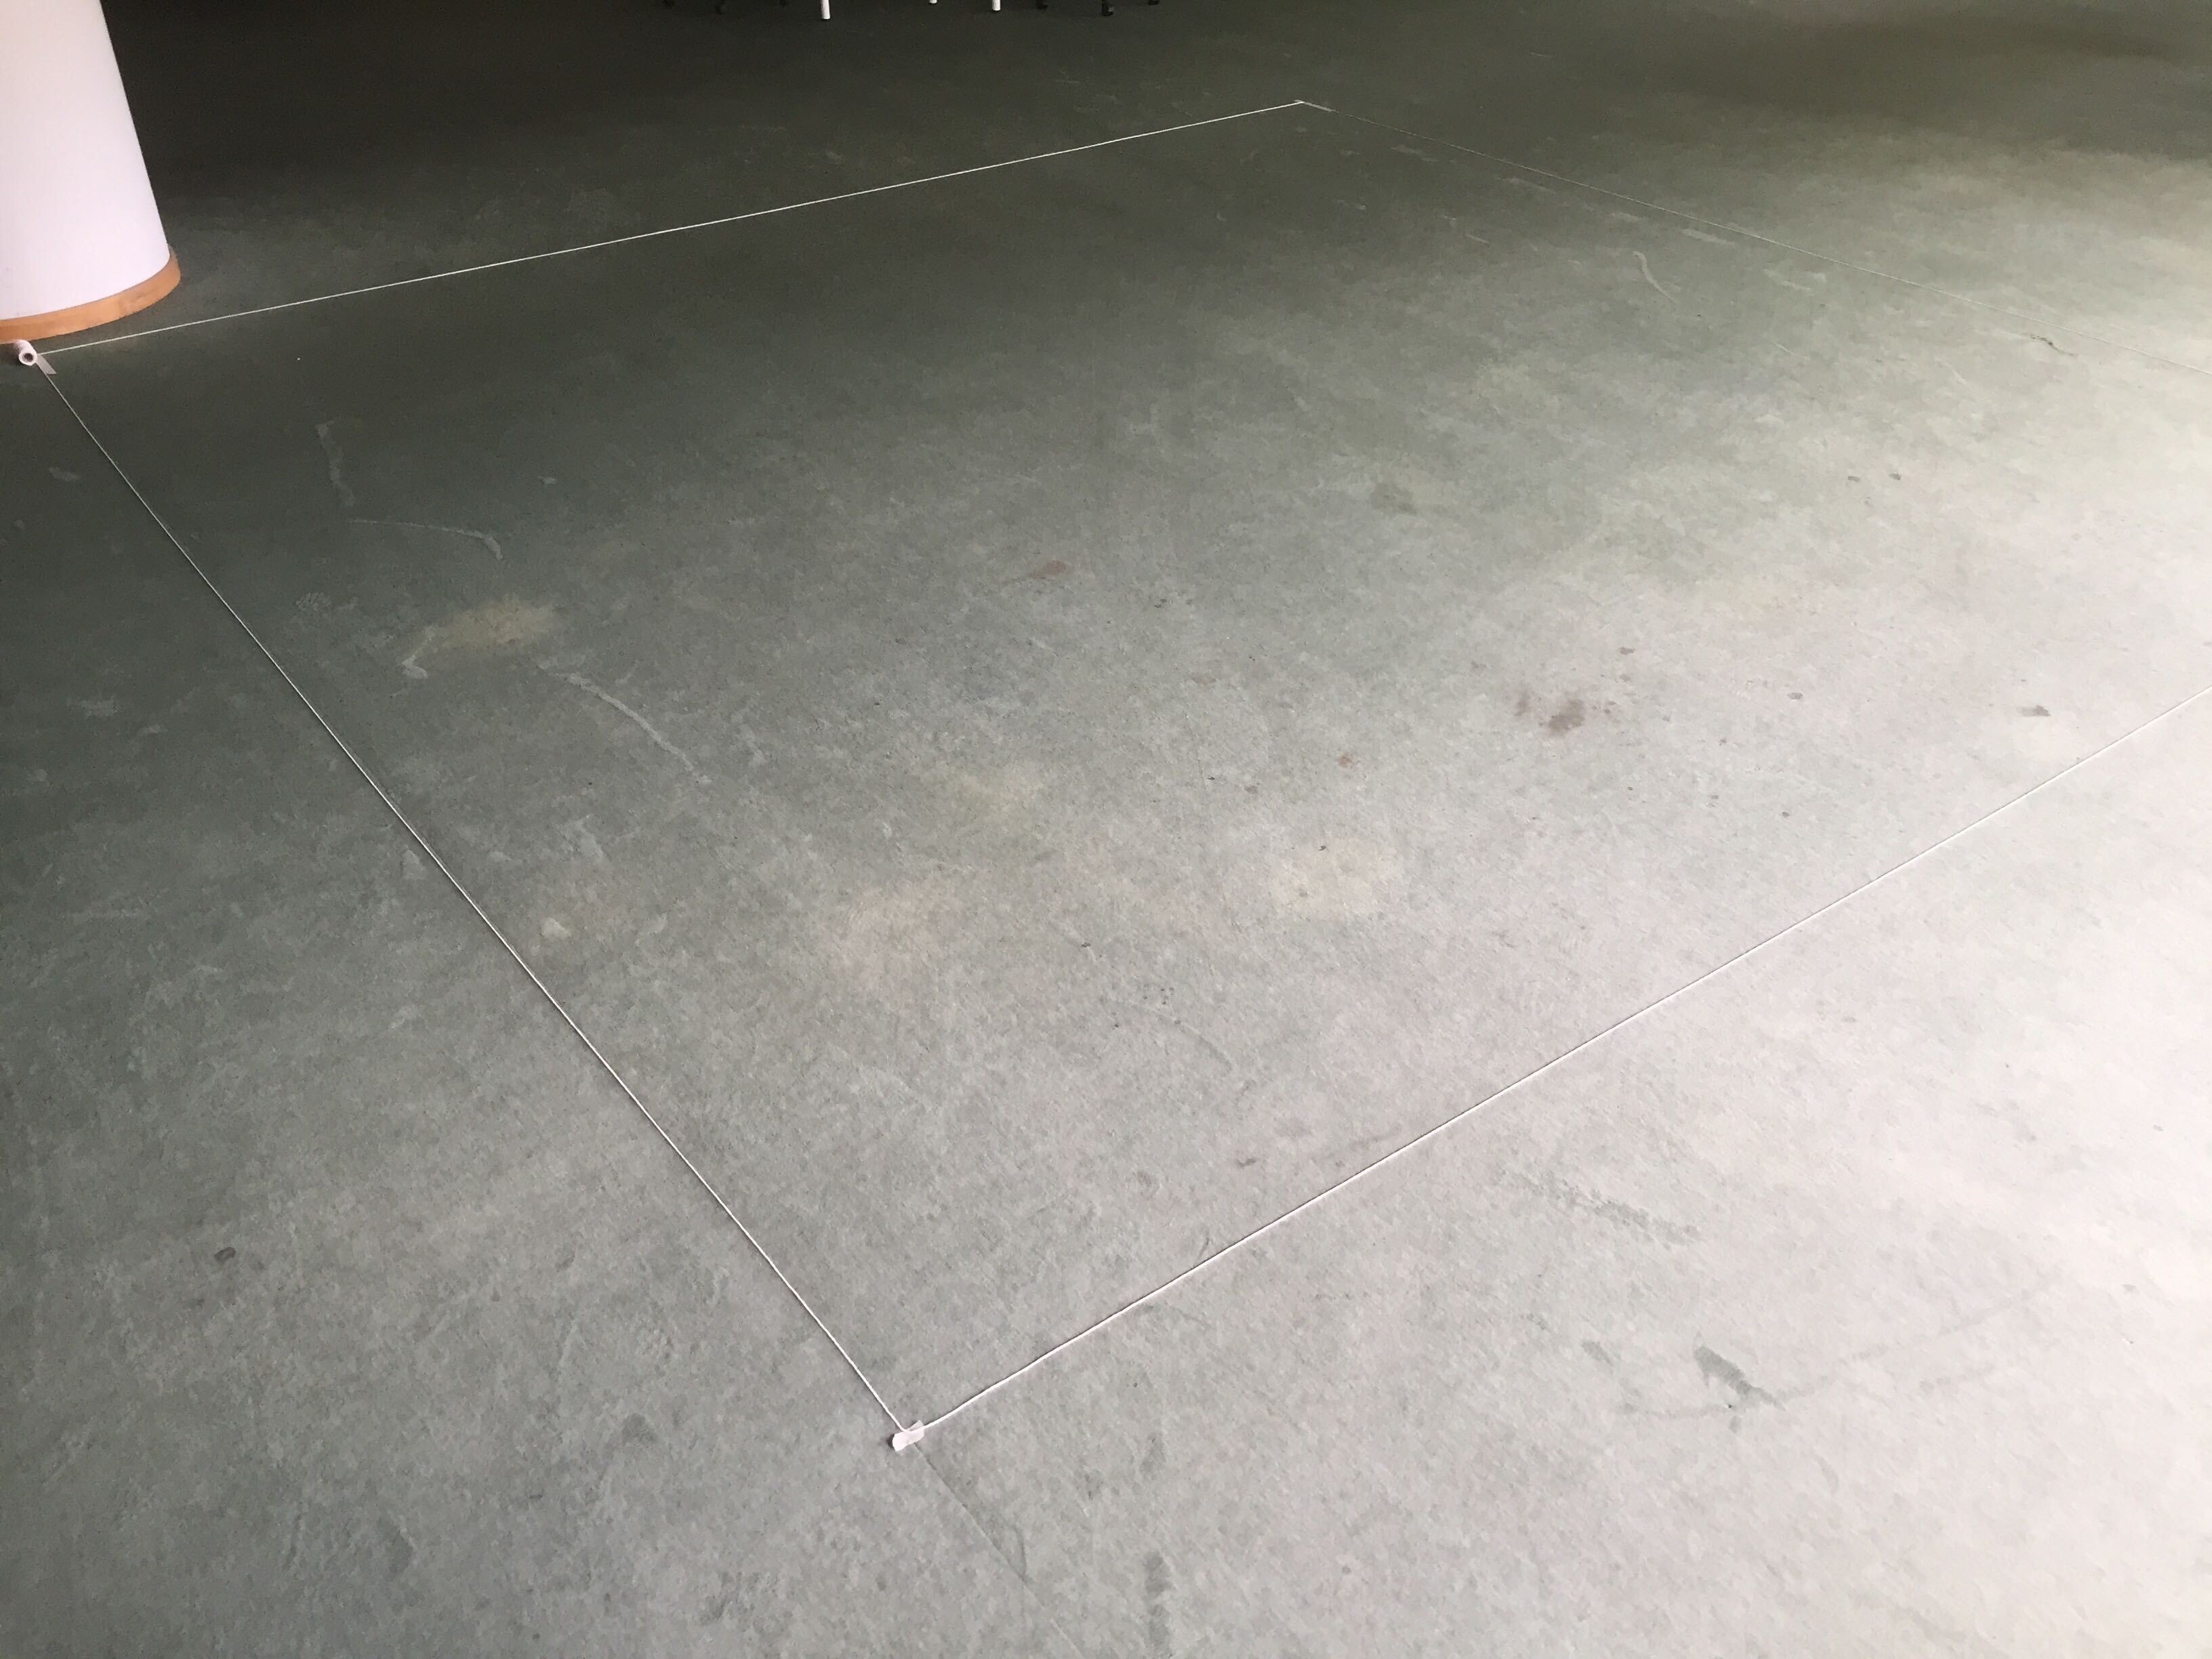
\includegraphics[width=0.475\textwidth]{figures/experiment2.jpg}
    \caption{ 5 meter side ground square used for baseline of accuracy of inertial system. }
    \label{fig:full}
\end{figure}

\begin{figure}[!h]
    \centering
    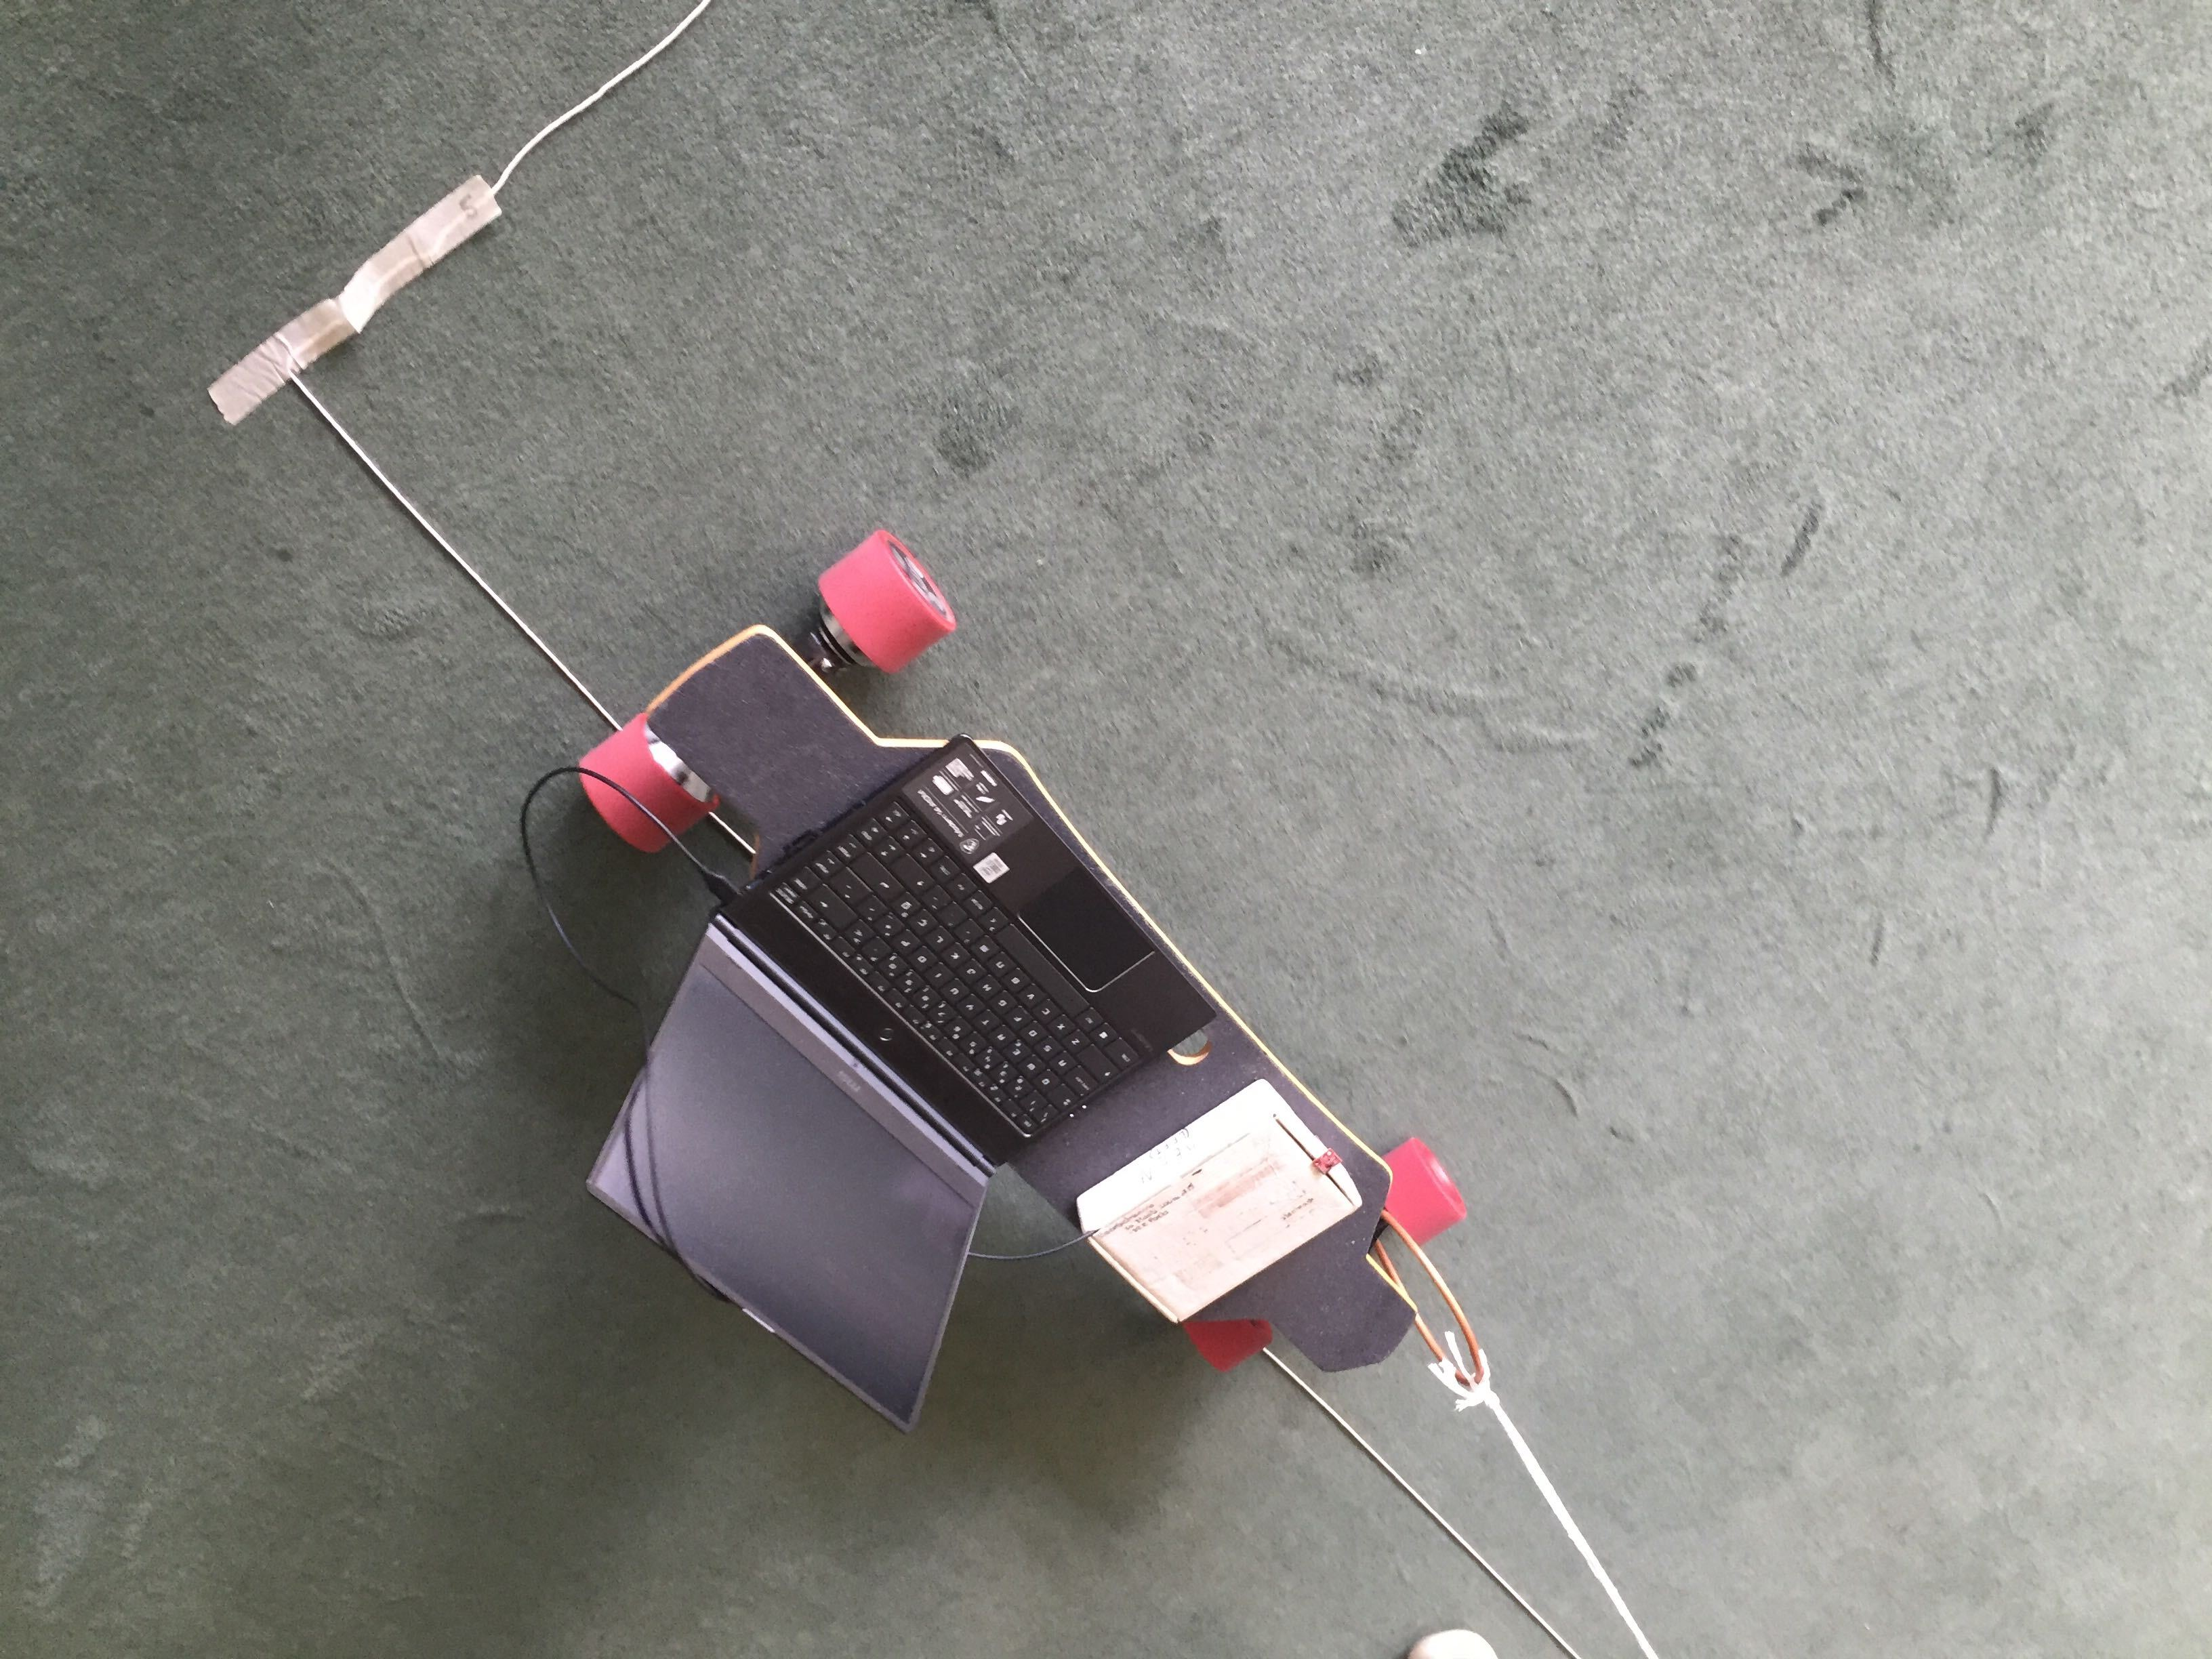
\includegraphics[width=0.475\textwidth]{figures/experiment3.jpg}
    \caption{ Experiment made with skateboard to assess localization accuracy. }
    \label{fig:full}
\end{figure}

\begin{figure}[!h]
    \centering
    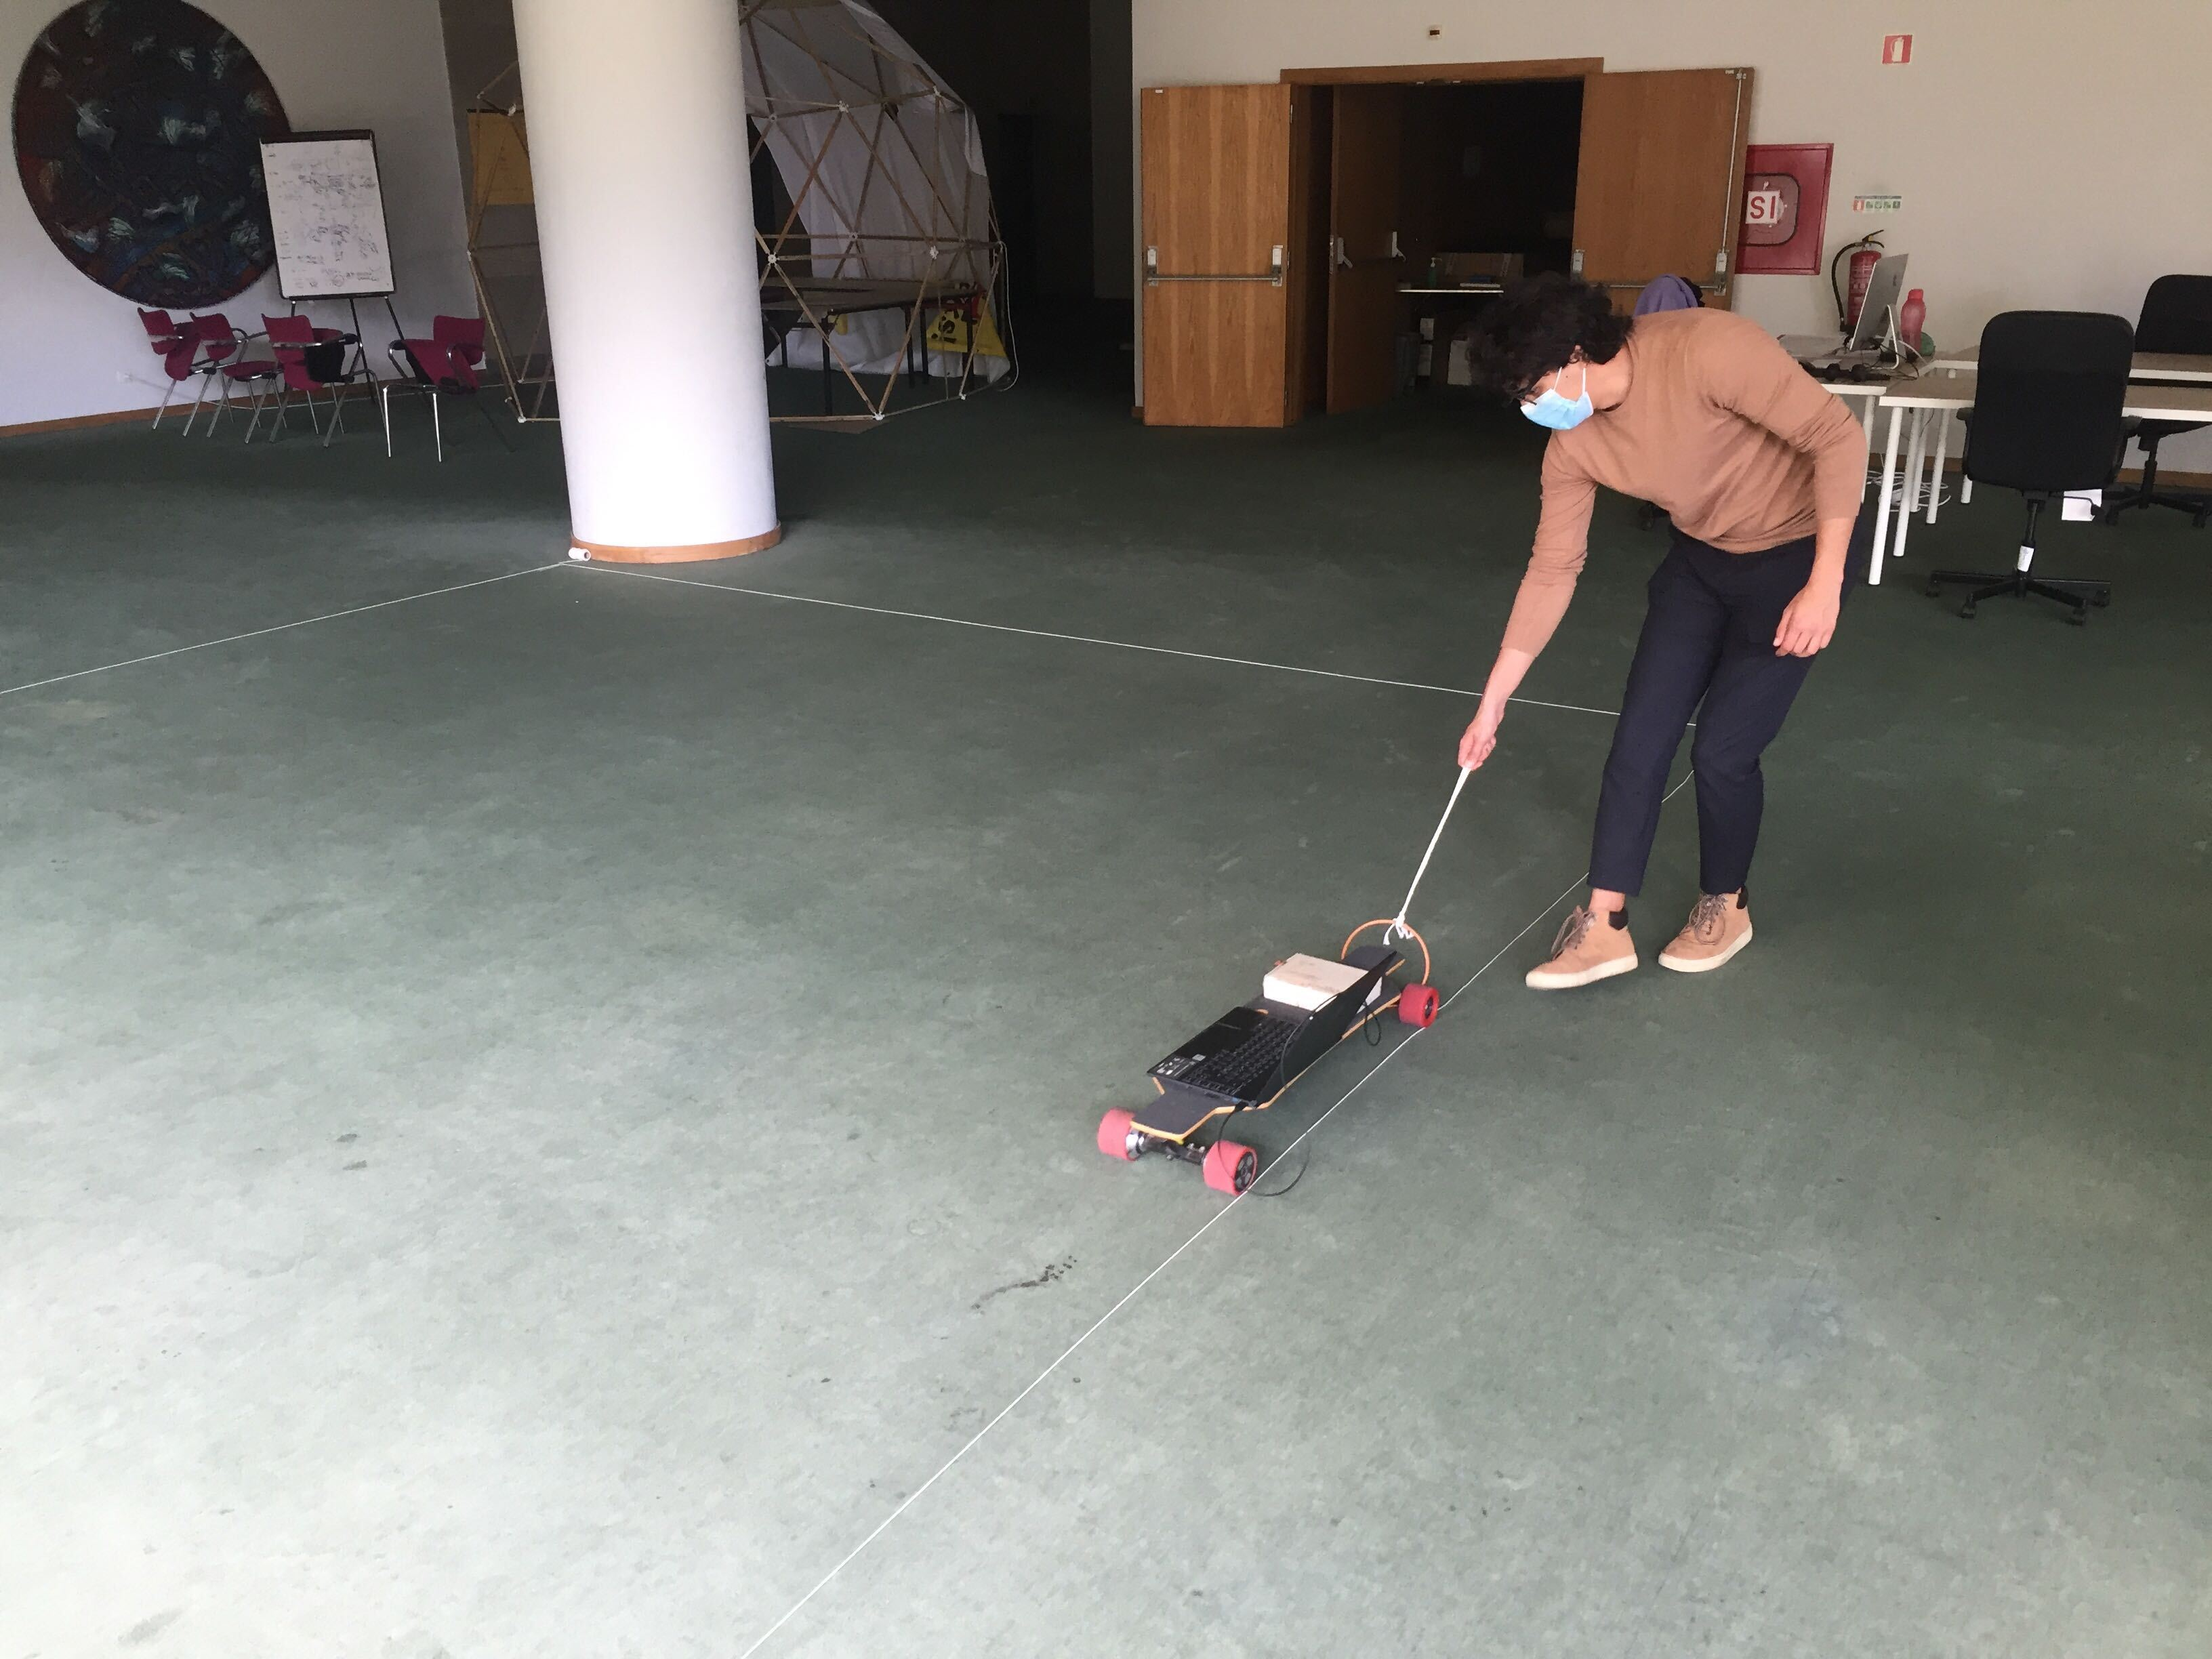
\includegraphics[width=0.475\textwidth]{figures/experiment.jpg}
    \caption{ Manually pulling the skateboard on each side of the ground square. }
    \label{fig:full}
\end{figure}

Finally, only the three-dimensional experiment was left combining the output readings from the Z-axis accelerometer. The same previous procedure was employed in this experimentation; the output from X-axis, Y-axis, and Z-axis accelerometer measurements were combined with orientation and integrated to obtain an accumulative position on all axes. A similar movement to the two-dimensional test was performed, but this time wobbling the inertial unit vertically to better visualize the position variation on the Z-axis. An example of an experimental test conducted in three dimensions in visible is figure \ref{fig:3dimensions}.

\begin{figure}[!h]
    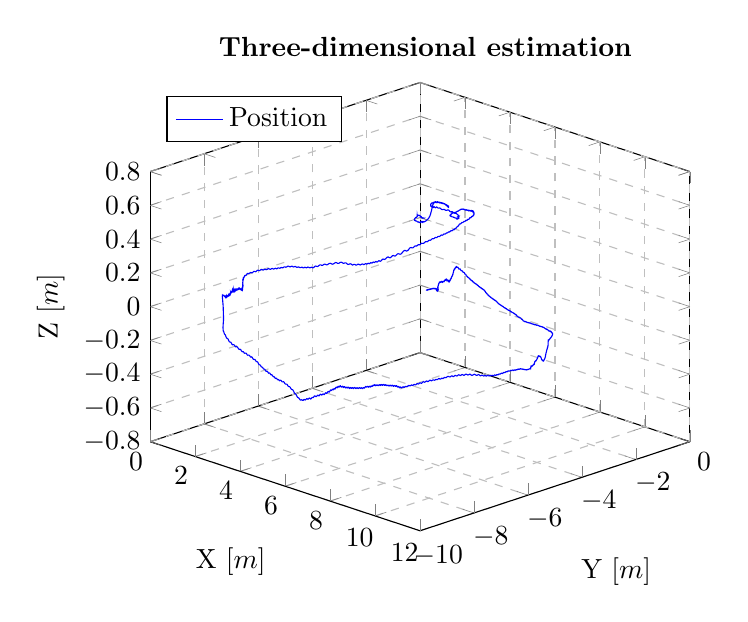
\begin{tikzpicture}
\begin{axis}[
    title={\textbf{ Three-dimensional estimation}},
    % view={-45}{60},
    view={45}{25},
    xlabel={X [$m$] },
    ylabel={Y [$m$] },
    zlabel={Z [$m$] },
    xmin=0, xmax=12,
    ymin=-10, ymax=0,
    zmin=-0.8, zmax=0.8,
    xtick distance = 2,
    ytick distance = 2,
    ztick distance = 0.2,
    % ytick={-80,-60,-40,-20,0,20,40,60,80,100},
    legend pos=north west,
    xmajorgrids=true,
    ymajorgrids=true,
    zmajorgrids=true,
    grid style=dashed,
]

\addplot3[
    color=blue
    ]
    coordinates {(0.02268617,0.1165467,-0.008550518)
(0.02266622,0.1165622,-0.008552011)
(0.02265028,0.1165747,-0.00855295)
(0.02263753,0.1165847,-0.008553559)
(0.02262731,0.1165926,-0.008553933)
(0.02261906,0.1165989,-0.008554117)
(0.02261241,0.1166038,-0.008554276)
(0.02260704,0.1166077,-0.008554445)
(0.02260273,0.1166108,-0.008554589)
(0.02259925,0.1166133,-0.008554658)
(0.02259648,0.1166152,-0.008554699)
(0.02259426,0.1166168,-0.008554791)
(0.02259251,0.1166181,-0.008554917)
(0.02259113,0.1166191,-0.008555043)
(0.02259004,0.11662,-0.00855512)
(0.02258919,0.1166207,-0.008555164)
(0.02258851,0.1166213,-0.008555201)
(0.02258797,0.1166217,-0.008555244)
(0.02258754,0.1166221,-0.008555275)
(0.02258719,0.1166224,-0.008555286)
(0.02258692,0.1166227,-0.008555291)
(0.02258671,0.1166229,-0.008555305)
(0.02258654,0.116623,-0.008555321)
(0.02258641,0.1166232,-0.008555339)
(0.02243895,0.1167889,-0.008570215)
(0.02221541,0.1170705,-0.008591964)
(0.02207642,0.1172553,-0.008604553)
(0.02196765,0.1174049,-0.008622352)
(0.0218829,0.1175262,-0.00863486)
(0.02181807,0.1176252,-0.008643769)
(0.02176982,0.1177067,-0.008650612)
(0.02173461,0.1177738,-0.008658289)
(0.02170951,0.117829,-0.008666327)
(0.02169229,0.1178743,-0.008673072)
(0.02160412,0.1181563,-0.008709674)
(0.02156155,0.1183214,-0.008728703)
(0.02153693,0.1184556,-0.00874309)
(0.02152326,0.1185638,-0.00875653)
(0.02151341,0.1189022,-0.008788559)
(0.02153966,0.1194397,-0.008816203)
(0.02158829,0.1197933,-0.008827213)
(0.0216654,0.1200682,-0.008841646)
(0.0218604,0.1205145,-0.008865004)
(0.02203903,0.1207989,-0.008896461)
(0.02220953,0.1210066,-0.008915668)
(0.02236636,0.1211536,-0.008919468)
(0.02250557,0.1212546,-0.008917418)
(0.02262371,0.1213251,-0.008918614)
(0.02272149,0.1213756,-0.008921898)
(0.02280147,0.1214125,-0.008919544)
(0.02286816,0.1214351,-0.008915314)
(0.02292223,0.121451,-0.008912872)
(0.02296619,0.121461,-0.008912858)
(0.02300169,0.1214674,-0.008912049)
(0.02303039,0.1214703,-0.00891227)
(0.02305344,0.1214715,-0.008910639)
(0.02307189,0.1214724,-0.008909261)
(0.0230866,0.1214737,-0.008908565)
(0.02309833,0.1214752,-0.008907826)
(0.02310775,0.121476,-0.008906962)
(0.02311531,0.1214763,-0.008906115)
(0.02312135,0.1214765,-0.008905928)
(0.02312619,0.1214767,-0.008905947)
(0.02313006,0.1214765,-0.008905914)
(0.02313316,0.1214763,-0.008905961)
(0.02313561,0.121476,-0.008905963)
(0.02313757,0.1214757,-0.008906001)
(0.02313915,0.1214755,-0.008905991)
(0.0231404,0.1214753,-0.00890605)
(0.02314139,0.1214751,-0.008906078)
(0.02314217,0.1214749,-0.00890609)
(0.02314279,0.1214747,-0.008906079)
(0.02314327,0.1214745,-0.008906099)
(0.02314364,0.1214743,-0.008906134)
(0.02314393,0.1214741,-0.008906154)
(0.02314414,0.121474,-0.008906158)
(0.02314431,0.1214738,-0.008906158)
(0.02314444,0.1214737,-0.008906167)
(0.02314454,0.1214736,-0.008906178)
(0.02314461,0.1214736,-0.008906179)
(0.02314467,0.1214735,-0.008906175)
(0.02314471,0.1214734,-0.00890617)
(0.02314475,0.1214734,-0.008906166)
(0.02314477,0.1214734,-0.008906165)
(0.02314479,0.1214733,-0.008906164)
(0.02314481,0.1214733,-0.008906162)
(0.02314481,0.1214733,-0.008906159)
(0.02314482,0.1214733,-0.008906157)
(0.0232311,0.1212114,-0.008875552)
(0.02327115,0.1210699,-0.008860873)
(0.02334947,0.1207286,-0.008829537)
(0.02338965,0.1205062,-0.008809229)
(0.0234454,0.1200537,-0.008764562)
(0.02348639,0.1193749,-0.008695193)
(0.02348813,0.1183968,-0.008620037)
(0.02340939,0.1171485,-0.008537749)
(0.02329083,0.116264,-0.008456032)
(0.02304482,0.1150793,-0.008342386)
(0.02261048,0.1135167,-0.008222569)
(0.02194307,0.1116062,-0.008131022)
(0.02111448,0.1096627,-0.00803304)
(0.02038808,0.1082198,-0.007940473)
(0.01945169,0.106623,-0.007825946)
(0.01824231,0.1048606,-0.007707226)
(0.01681283,0.1030639,-0.007594285)
(0.0151116,0.1012377,-0.007506414)
(0.01370669,0.09993123,-0.007427323)
(0.0120659,0.09860769,-0.007338915)
(0.009919396,0.09708479,-0.007331791)
(0.007474994,0.09555491,-0.007430416)
(0.005559563,0.09449814,-0.007457609)
(0.003986118,0.09373191,-0.007442167)
(0.002698981,0.09318102,-0.007415046)
(0.001158522,0.09260756,-0.007419446)
(-0.0005821338,0.09210099,-0.007478783)
(-0.002814684,0.091555,-0.007419373)
(-0.004465724,0.09120872,-0.007346048)
(-0.00656251,0.09084869,-0.007305125)
(-0.00883724,0.09053433,-0.00733603)
(-0.01150723,0.09024973,-0.007488169)
(-0.01351951,0.09012154,-0.007642934)
(-0.01580924,0.0901195,-0.00787837)
(-0.01756312,0.0902521,-0.008029106)
(-0.01949003,0.09058493,-0.008162807)
(-0.02155924,0.09112159,-0.008262863)
(-0.02311317,0.0916585,-0.008323072)
(-0.02492913,0.09238049,-0.008340458)
(-0.02628422,0.09297726,-0.008330372)
(-0.0273526,0.09348882,-0.008312078)
(-0.02818081,0.09394932,-0.00831794)
(-0.02881747,0.09436089,-0.008352223)
(-0.02930501,0.09472162,-0.008398872)
(-0.02967313,0.09503767,-0.008445614)
(-0.02994862,0.09531111,-0.008504743)
(-0.03041599,0.09584413,-0.008583735)
(-0.0310235,0.09664479,-0.008637695)
(-0.03162341,0.09759294,-0.008701253)
(-0.03202334,0.09832089,-0.008759426)
(-0.03251345,0.09939626,-0.00879397)
(-0.03305685,0.1007382,-0.008736914)
(-0.03340076,0.1017367,-0.008712179)
(-0.03365007,0.1025439,-0.008755614)
(-0.03382952,0.1031955,-0.008816177)
(-0.03396114,0.10372,-0.008863499)
(-0.03406251,0.1041405,-0.008911925)
(-0.03414018,0.1044777,-0.008955149)
(-0.03425813,0.1050248,-0.009010421)
(-0.03432374,0.10541,-0.009047832)
(-0.03440318,0.1061356,-0.009077178)
(-0.03442814,0.1070897,-0.009041225)
(-0.03438316,0.1081489,-0.009014301)
(-0.034293,0.1089337,-0.009034676)
(-0.03417538,0.1095546,-0.009098404)
(-0.03405364,0.1100452,-0.00914546)
(-0.03391817,0.1104263,-0.009187661)
(-0.03368807,0.1110085,-0.009275985)
(-0.03350497,0.1114105,-0.009380961)
(-0.03333749,0.1117217,-0.009465571)
(-0.03293219,0.1123552,-0.009564874)
(-0.0323602,0.1130462,-0.009597947)
(-0.03191301,0.113509,-0.009598018)
(-0.03119646,0.1141165,-0.009508013)
(-0.03064919,0.1145076,-0.009478665)
(-0.02990748,0.1149668,-0.009498044)
(-0.02933232,0.1152578,-0.009544778)
(-0.02886141,0.115468,-0.009583417)
(-0.02810361,0.1157861,-0.009698254)
(-0.02759128,0.116049,-0.009774043)
(-0.02718354,0.1162634,-0.009832875)
(-0.02648487,0.1165774,-0.00985464)
(-0.02598156,0.1167477,-0.009832083)
(-0.02557331,0.1168662,-0.009801764)
(-0.02482042,0.1170662,-0.009778583)
(-0.02430788,0.1171963,-0.009816149)
(-0.02389703,0.1172972,-0.009830231)
(-0.02356865,0.1173791,-0.009818021)
(-0.02330534,0.1174422,-0.009822175)
(-0.02271249,0.117609,-0.009925334)
(-0.0223368,0.1177483,-0.01000159)
(-0.02204015,0.1178697,-0.01001641)
(-0.02180274,0.1179666,-0.01000542)
(-0.02160494,0.118021,-0.009993872)
(-0.02120449,0.1181024,-0.009949286)
(-0.02093414,0.1181378,-0.009931951)
(-0.02071684,0.1181567,-0.009912127)
(-0.02054238,0.1181533,-0.009898365)
(-0.0199965,0.1181141,-0.009900772)
(-0.01910633,0.1180123,-0.009996343)
(-0.01817335,0.1178828,-0.01015567)
(-0.01749017,0.1177337,-0.01025746)
(-0.01695023,0.1175874,-0.01029008)
(-0.01652671,0.1174429,-0.01028795)
(-0.0161914,0.1173174,-0.01028326)
(-0.01592742,0.1172063,-0.01027173)
(-0.01547893,0.1169907,-0.01025944)
(-0.01518567,0.1168152,-0.01024119)
(-0.01467361,0.1164251,-0.01019749)
(-0.01392419,0.1157256,-0.01014759)
(-0.01291348,0.1145881,-0.01014393)
(-0.01229284,0.113751,-0.01010163)
(-0.01184639,0.1130469,-0.01001584)
(-0.01152322,0.1124635,-0.009914122)
(-0.01110397,0.1116426,-0.00970152)
(-0.01082369,0.1110346,-0.009527829)
(-0.0104817,0.1101954,-0.009305813)
(-0.01009199,0.1090426,-0.009063311)
(-0.009620901,0.1071856,-0.008799635)
(-0.009209179,0.1049217,-0.008608011)
(-0.008935454,0.1023444,-0.008471514)
(-0.008865163,0.1004085,-0.008328465)
(-0.008916196,0.09885965,-0.008179966)
(-0.009063993,0.09712352,-0.007935728)
(-0.009289657,0.09505715,-0.007497246)
(-0.009487518,0.09351366,-0.007121007)
(-0.009770843,0.09171524,-0.006710181)
(-0.01016679,0.08977438,-0.006295877)
(-0.01082624,0.08729574,-0.005887611)
(-0.01172572,0.08460272,-0.005521305)
(-0.01294068,0.08158237,-0.005240758)
(-0.01397503,0.07936219,-0.005001027)
(-0.01489702,0.07763323,-0.004799012)
(-0.01569629,0.07628477,-0.004587999)
(-0.01638178,0.07523466,-0.004402308)
(-0.0169654,0.07441866,-0.004229496)
(-0.01745846,0.0737854,-0.004071408)
(-0.01812254,0.07298336,-0.003885277)
(-0.01902892,0.07196646,-0.003671269)
(-0.02023647,0.07073322,-0.003455109)
(-0.02205665,0.06905151,-0.003324089)
(-0.02342764,0.06798374,-0.003277686)
(-0.02500959,0.06688254,-0.003190341)
(-0.02677365,0.06576198,-0.003033375)
(-0.02897586,0.06445718,-0.002708434)
(-0.03064854,0.06355088,-0.002467232)
(-0.03283156,0.06248108,-0.002219916)
(-0.03526314,0.06138975,-0.002038394)
(-0.03786093,0.06046796,-0.001929286)
(-0.03993205,0.05991222,-0.001880117)
(-0.04162046,0.05960852,-0.001871811)
(-0.04298592,0.05947065,-0.00185827)
(-0.04408341,0.05943976,-0.001831065)
(-0.04546241,0.05950097,-0.001769953)
(-0.04709745,0.0596714,-0.001645415)
(-0.04829982,0.05987649,-0.001534093)
(-0.04925186,0.06009045,-0.001448973)
(-0.05000095,0.06031012,-0.001370593)
(-0.05096508,0.06066829,-0.001350907)
(-0.05165212,0.06098547,-0.001378067)
(-0.05218095,0.06128011,-0.001423494)
(-0.05289555,0.06174945,-0.001473417)
(-0.05339366,0.06211424,-0.001508048)
(-0.05377834,0.06242406,-0.001527565)
(-0.05435316,0.06293294,-0.001532743)
(-0.05510436,0.06365346,-0.001469442)
(-0.05591193,0.06456233,-0.001366887)
(-0.05676162,0.06567847,-0.001261196)
(-0.05734988,0.06654339,-0.001239665)
(-0.05780243,0.06724726,-0.001250491)
(-0.05815145,0.06781852,-0.001244061)
(-0.0584211,0.06828123,-0.001256159)
(-0.05863328,0.06865345,-0.001265339)
(-0.05880087,0.06895244,-0.001275407)
(-0.0590584,0.06943696,-0.00127991)
(-0.05938634,0.07011616,-0.001246501)
(-0.05959082,0.07060542,-0.001213517)
(-0.05973044,0.071006,-0.001198705)
(-0.0598264,0.07133152,-0.0011936)
(-0.05988907,0.07159569,-0.001211096)
(-0.05993867,0.07180715,-0.001225978)
(-0.06002735,0.07225385,-0.001244887)
(-0.06009877,0.07294559,-0.001232922)
(-0.06011222,0.07341656,-0.00122979)
(-0.06010283,0.07379336,-0.00123129)
(-0.06008031,0.07409406,-0.001243035)
(-0.06000023,0.07460573,-0.001258267)
(-0.05975539,0.07545736,-0.001292259)
(-0.0592946,0.07651741,-0.001336366)
(-0.05866688,0.07760655,-0.001428617)
(-0.05810782,0.07836428,-0.001557362)
(-0.05717196,0.07937752,-0.001711878)
(-0.05601954,0.08035229,-0.001840271)
(-0.05461436,0.08125813,-0.001906624)
(-0.0534667,0.08180111,-0.001925025)
(-0.0524965,0.08210174,-0.001933882)
(-0.05169287,0.08222185,-0.001895781)
(-0.05104282,0.08222256,-0.001852257)
(-0.0502152,0.08201567,-0.001796986)
(-0.04928271,0.08163318,-0.001745458)
(-0.04824851,0.08104323,-0.001682226)
(-0.04753543,0.08052076,-0.001610512)
(-0.04672284,0.07979112,-0.001532007)
(-0.04615627,0.07920084,-0.001461532)
(-0.04573205,0.07870236,-0.001407495)
(-0.04541102,0.07828868,-0.001369551)
(-0.04516536,0.07794936,-0.001340256)
(-0.04497562,0.07767311,-0.001318003)
(-0.04482327,0.07745251,-0.001301178)
(-0.04469981,0.07727713,-0.00128915)
(-0.0445999,0.07713762,-0.001280281)
(-0.04451935,0.07702647,-0.001272763)
(-0.04445457,0.0769378,-0.001267638)
(-0.04440425,0.07686579,-0.001264964)
(-0.04436491,0.07680755,-0.00126297)
(-0.04433368,0.07676079,-0.001259947)
(-0.04411823,0.07644344,-0.001203827)
(-0.04399337,0.07626285,-0.001155354)
(-0.043293,0.07526808,-0.0007270894)
(-0.04236738,0.07395243,-0.0002135798)
(-0.04089942,0.07161857,0.0002837252)
(-0.03942793,0.06902242,0.0005459384)
(-0.03806574,0.06631717,0.0006893672)
(-0.03708229,0.06418306,0.0007550143)
(-0.03631928,0.06246503,0.0008881407)
(-0.0357188,0.06108624,0.001011154)
(-0.03520012,0.0600007,0.001135577)
(-0.03446144,0.05864275,0.001434113)
(-0.03336863,0.05693247,0.00208642)
(-0.03256716,0.05570709,0.00260918)
(-0.03104833,0.05334509,0.003222333)
(-0.02924969,0.05030831,0.003494346)
(-0.02770954,0.04730266,0.003650482)
(-0.02657408,0.04492101,0.003809252)
(-0.02571621,0.04299242,0.003934329)
(-0.02506025,0.04143641,0.004073896)
(-0.02426534,0.03968985,0.004339683)
(-0.02329643,0.03785944,0.004730376)
(-0.02205467,0.03602635,0.00528535)
(-0.02067052,0.03415158,0.005998942)
(-0.01891731,0.03177953,0.006701677)
(-0.01672974,0.02847457,0.007135747)
(-0.01467021,0.02477806,0.00731885)
(-0.01286013,0.02096158,0.007524861)
(-0.01113797,0.0167207,0.007657269)
(-0.00997841,0.01336749,0.007763585)
(-0.008915835,0.009721052,0.008043636)
(-0.007850659,0.005773252,0.008653704)
(-0.006670957,0.001633685,0.009454456)
(-0.005331248,-0.002663635,0.01043893)
(-0.003885704,-0.007222232,0.01175083)
(-0.002228644,-0.01239125,0.01284075)
(-0.0004526172,-0.01852028,0.01327175)
(0.001116815,-0.02460872,0.01333683)
(0.00225571,-0.02942317,0.01330655)
(0.002945247,-0.03332049,0.0134471)
(0.003442708,-0.03644744,0.01370469)
(0.004064688,-0.03976883,0.01409654)
(0.00488351,-0.04321993,0.01465136)
(0.005911067,-0.04695384,0.01559301)
(0.006774922,-0.0498164,0.01625162)
(0.007742461,-0.05319745,0.01678779)
(0.008858858,-0.05751469,0.01694426)
(0.009798635,-0.06184347,0.01689354)
(0.01042461,-0.06523847,0.01685145)
(0.01081585,-0.06797238,0.01680985)
(0.01108359,-0.07016552,0.01685364)
(0.01131145,-0.07191831,0.01693826)
(0.01166129,-0.0738751,0.01714401)
(0.01213486,-0.07609683,0.01754974)
(0.01269902,-0.07849389,0.01813632)
(0.01358713,-0.08152143,0.01856538)
(0.0145355,-0.08478251,0.01867324)
(0.01543118,-0.08819143,0.01858701)
(0.01606041,-0.09085866,0.01859284)
(0.01648763,-0.09300899,0.0186062)
(0.01675542,-0.09474231,0.01870702)
(0.01699372,-0.09612502,0.01884021)
(0.0173203,-0.09771654,0.01907754)
(0.01784745,-0.09945731,0.01943005)
(0.01857876,-0.1012887,0.01987217)
(0.01917571,-0.102679,0.02023736)
(0.02010605,-0.104842,0.02047736)
(0.02113697,-0.1075043,0.02044635)
(0.02179283,-0.1094737,0.02039474)
(0.02221086,-0.1110808,0.0203709)
(0.0224755,-0.1123826,0.02041189)
(0.02265127,-0.1134308,0.02044748)
(0.02278988,-0.1142696,0.02049469)
(0.02300328,-0.1153228,0.02061736)
(0.02328371,-0.1164843,0.02081512)
(0.02354075,-0.1173508,0.0209503)
(0.02423001,-0.1195208,0.02092835)
(0.02518711,-0.1222357,0.02044867)
(0.02600327,-0.1240839,0.02000019)
(0.02670943,-0.1255378,0.01964149)
(0.02722334,-0.1267243,0.01945306)
(0.02787308,-0.1281003,0.01934412)
(0.02847406,-0.1290883,0.01928401)
(0.02940574,-0.1303084,0.01932063)
(0.03066506,-0.1316584,0.0195747)
(0.03206151,-0.132936,0.01981931)
(0.03431726,-0.1349136,0.01974564)
(0.03681013,-0.1371369,0.0191883)
(0.03861195,-0.1388371,0.01874276)
(0.04000799,-0.1402438,0.01855853)
(0.0410718,-0.1414194,0.01844149)
(0.04191045,-0.142371,0.01843808)
(0.04261326,-0.1431029,0.01841992)
(0.04362516,-0.1439179,0.01847884)
(0.04444406,-0.1444256,0.01855536)
(0.04512959,-0.1447781,0.01865699)
(0.04623119,-0.1453481,0.01864174)
(0.04760445,-0.1460845,0.01826183)
(0.04904986,-0.146946,0.01773725)
(0.05050821,-0.1479769,0.01730261)
(0.05204279,-0.149185,0.017117)
(0.05320228,-0.1501371,0.01703113)
(0.05413832,-0.1508884,0.01688689)
(0.05489616,-0.151478,0.01686418)
(0.05598413,-0.1523072,0.01697444)
(0.05674292,-0.1529362,0.01708536)
(0.05834662,-0.1543385,0.01701046)
(0.06030101,-0.1562656,0.0166089)
(0.06218364,-0.15852,0.01612635)
(0.06345249,-0.1603292,0.01592541)
(0.06484547,-0.1627182,0.01555059)
(0.06606345,-0.1652803,0.0153658)
(0.06714098,-0.1680956,0.01523907)
(0.06786633,-0.1703219,0.01527066)
(0.06840554,-0.1721158,0.01537786)
(0.06914618,-0.1746877,0.01589174)
(0.07012949,-0.177974,0.0163974)
(0.07151255,-0.1828852,0.01636648)
(0.07262936,-0.1880505,0.0159456)
(0.07345154,-0.193532,0.01524531)
(0.07391582,-0.1991428,0.01461074)
(0.07396681,-0.2035751,0.01431404)
(0.07386261,-0.2071196,0.01416359)
(0.07373418,-0.2099535,0.01416053)
(0.07361239,-0.2130201,0.01437922)
(0.0735405,-0.2162779,0.01472032)
(0.07357589,-0.2196411,0.01521238)
(0.07356681,-0.2240722,0.01522994)
(0.07348912,-0.2293417,0.01449005)
(0.07329449,-0.2347494,0.01324829)
(0.07305793,-0.2389259,0.01222971)
(0.0727708,-0.2422601,0.01166126)
(0.0725167,-0.2449253,0.01131214)
(0.07236738,-0.2470619,0.01106835)
(0.07224745,-0.2494055,0.01091212)
(0.07221795,-0.2520922,0.01100714)
(0.07242381,-0.2549422,0.01107544)
(0.07281672,-0.257111,0.01107403)
(0.07333903,-0.2595502,0.01077126)
(0.07397026,-0.2627266,0.009918345)
(0.07437755,-0.2650578,0.009180955)
(0.07470722,-0.2669222,0.008631589)
(0.07504228,-0.2683993,0.008238307)
(0.07531033,-0.269581,0.007913785)
(0.07568936,-0.2709508,0.007578647)
(0.07625759,-0.2726637,0.007259948)
(0.07709631,-0.274492,0.006909816)
(0.07833701,-0.2764208,0.006606679)
(0.08000182,-0.278396,0.00637084)
(0.08143514,-0.2797236,0.006111655)
(0.08359974,-0.2813639,0.005463901)
(0.08597967,-0.2827368,0.004602083)
(0.08795286,-0.2835169,0.003934608)
(0.09026632,-0.2840778,0.003324386)
(0.09289145,-0.2841922,0.002874594)
(0.0948985,-0.2840353,0.002558935)
(0.09708603,-0.283666,0.002443712)
(0.09874365,-0.2832069,0.002404116)
(0.1000408,-0.2827477,0.002469988)
(0.1016832,-0.2821133,0.0026505)
(0.1033905,-0.2813866,0.002919576)
(0.1059891,-0.2801873,0.002933495)
(0.1096588,-0.2784147,0.002336871)
(0.1130347,-0.2765771,0.001501117)
(0.115632,-0.2750819,0.001060462)
(0.1176972,-0.2738642,0.000976655)
(0.1200531,-0.2723784,0.001267351)
(0.1217526,-0.271103,0.001488814)
(0.1243118,-0.26894,0.001519836)
(0.1273875,-0.2660882,0.001030698)
(0.1307253,-0.2626011,-0.0001191403)
(0.1336715,-0.2589255,-0.001158425)
(0.1366459,-0.2547291,-0.001740908)
(0.1396502,-0.2501544,-0.001839195)
(0.1417921,-0.2464892,-0.001874001)
(0.1440299,-0.242462,-0.002253668)
(0.1465604,-0.2376139,-0.003258389)
(0.1488633,-0.2324152,-0.004771056)
(0.1508639,-0.2269929,-0.006174866)
(0.1527052,-0.2210479,-0.007180318)
(0.154397,-0.2149542,-0.007820997)
(0.1555321,-0.2101003,-0.008197066)
(0.1565562,-0.2044465,-0.008153559)
(0.1572221,-0.198666,-0.007922328)
(0.1576685,-0.1918882,-0.008167325)
(0.1577787,-0.1842824,-0.00930081)
(0.1574756,-0.1764364,-0.01110814)
(0.1568968,-0.1703522,-0.01272946)
(0.1560864,-0.1636268,-0.0141194)
(0.1550448,-0.1564741,-0.01497237)
(0.1537615,-0.1489012,-0.0152414)
(0.1520957,-0.1407055,-0.01480355)
(0.1500249,-0.1323101,-0.01383997)
(0.1470283,-0.1224948,-0.01383099)
(0.143154,-0.1118867,-0.0150038)
(0.1396521,-0.1040332,-0.01611439)
(0.1355703,-0.09616678,-0.01755334)
(0.132022,-0.09010998,-0.01877365)
(0.1280024,-0.08400773,-0.01989652)
(0.1235727,-0.07777922,-0.02075556)
(0.1188276,-0.07133638,-0.02116204)
(0.1138495,-0.06483921,-0.02116012)
(0.1084715,-0.05818257,-0.02065766)
(0.1026232,-0.05129461,-0.01948718)
(0.0960343,-0.04403957,-0.01855354)
(0.08845067,-0.03608695,-0.01878289)
(0.0805016,-0.02811064,-0.01984535)
(0.0741639,-0.02200315,-0.02074665)
(0.06756259,-0.01562287,-0.02130669)
(0.06253009,-0.01041312,-0.0216895)
(0.05874857,-0.006022274,-0.02193776)
(0.05506055,-0.001149721,-0.02181023)
(0.05219708,0.002708143,-0.02166719)
(0.04922853,0.006778016,-0.02135955)
(0.04570935,0.01175302,-0.02165391)
(0.04176454,0.01742323,-0.02276348)
(0.03798759,0.02301681,-0.0240914)
(0.03409745,0.02908108,-0.02521757)
(0.03035943,0.03535679,-0.02614613)
(0.02664252,0.04197747,-0.0266687)
(0.02300559,0.04895766,-0.02674074)
(0.01942857,0.05613106,-0.02703509)
(0.01582413,0.06367177,-0.02778791)
(0.01151434,0.07216645,-0.02960846)
(0.008046366,0.07855633,-0.03114666)
(0.004300611,0.08513815,-0.03248124)
(0.0004815022,0.09181972,-0.03366457)
(-0.002607605,0.09707636,-0.03463192)
(-0.005988722,0.102492,-0.03546451)
(-0.009827293,0.1081329,-0.03598838)
(-0.01404084,0.1136804,-0.03627785)
(-0.0175587,0.1178916,-0.0364619)
(-0.0216317,0.1223855,-0.0369666)
(-0.02640624,0.12733,-0.03793187)
(-0.03156392,0.1322931,-0.03926952)
(-0.03683462,0.1371455,-0.04042125)
(-0.04244512,0.1420663,-0.04132789)
(-0.04826816,0.1469683,-0.04202146)
(-0.05463135,0.1521892,-0.04231548)
(-0.0614254,0.1575771,-0.04202496)
(-0.06875453,0.1631692,-0.04086076)
(-0.07629499,0.1685728,-0.03993276)
(-0.08456508,0.174175,-0.03979419)
(-0.09320354,0.179816,-0.0402858)
(-0.09997761,0.1842451,-0.04082094)
(-0.1052986,0.1879343,-0.04122629)
(-0.1106774,0.1922336,-0.04145375)
(-0.114742,0.1957874,-0.04159927)
(-0.1189866,0.1995942,-0.04158405)
(-0.123649,0.2039178,-0.0410532)
(-0.127128,0.2073467,-0.0407445)
(-0.1310474,0.2115885,-0.04101097)
(-0.1347992,0.2163653,-0.0420853)
(-0.1378044,0.2217812,-0.04335945)
(-0.1403478,0.2280566,-0.04426365)
(-0.1421806,0.2349689,-0.04475918)
(-0.1432348,0.2424931,-0.04451428)
(-0.1433568,0.250077,-0.04431014)
(-0.1429716,0.2560783,-0.04410042)
(-0.1424959,0.2631664,-0.04475898)
(-0.1421766,0.2703749,-0.04584087)
(-0.1419092,0.2776508,-0.04633943)
(-0.1411829,0.2853205,-0.04605374)
(-0.1397339,0.293425,-0.04480898)
(-0.1380158,0.2995912,-0.04387808)
(-0.1357879,0.307375,-0.0440962)
(-0.13429,0.3132109,-0.04423813)
(-0.1325039,0.3200322,-0.04335481)
(-0.1312146,0.3252424,-0.04224522)
(-0.1294861,0.332809,-0.04183898)
(-0.12816,0.3399376,-0.04123076)
(-0.12681,0.347623,-0.0398028)
(-0.1256668,0.3556078,-0.03873978)
(-0.1247422,0.3651801,-0.03861909)
(-0.1246054,0.3747503,-0.03870277)
(-0.1248985,0.3854027,-0.03745595)
(-0.1255432,0.3960527,-0.03527639)
(-0.1269742,0.4078173,-0.0339229)
(-0.1293344,0.420185,-0.03352633)
(-0.1325017,0.4322179,-0.03252922)
(-0.1361662,0.4449008,-0.03013017)
(-0.1393868,0.4547234,-0.02779717)
(-0.1436068,0.4658209,-0.02647966)
(-0.1486172,0.4771688,-0.0261444)
(-0.1540798,0.4882728,-0.02520706)
(-0.1599695,0.5001571,-0.02280195)
(-0.1661023,0.5118141,-0.02038264)
(-0.173307,0.5243315,-0.01882052)
(-0.1812342,0.5367848,-0.01817543)
(-0.1898627,0.5493446,-0.01644276)
(-0.1988874,0.5621613,-0.0133822)
(-0.2063112,0.5720416,-0.01074866)
(-0.2146879,0.5827964,-0.009473285)
(-0.2233876,0.5936294,-0.009469658)
(-0.23224,0.6045945,-0.00863007)
(-0.2413871,0.6162469,-0.006384051)
(-0.248469,0.6254603,-0.00452317)
(-0.2563187,0.6354452,-0.003698184)
(-0.2646997,0.6454673,-0.003809615)
(-0.2734389,0.6555328,-0.003403255)
(-0.2826039,0.6662363,-0.001489239)
(-0.2898743,0.6745242,0.0003724219)
(-0.2981632,0.6836611,0.0008793771)
(-0.3064675,0.6925925,0.0008597773)
(-0.3150282,0.702202,0.002140764)
(-0.3232811,0.7124001,0.004349596)
(-0.3318237,0.7228589,0.005877405)
(-0.3411907,0.734094,0.005515101)
(-0.3486783,0.7426282,0.005467697)
(-0.3569284,0.7521439,0.007122856)
(-0.3631098,0.7596768,0.008693202)
(-0.3697464,0.7675829,0.009652871)
(-0.3771552,0.7761204,0.009270857)
(-0.3846447,0.7844679,0.009529996)
(-0.3927666,0.7937642,0.0114859)
(-0.4004558,0.8033682,0.01399952)
(-0.4085533,0.813583,0.01492245)
(-0.4171259,0.8243171,0.01420146)
(-0.4238741,0.8326549,0.01368957)
(-0.4309593,0.8419604,0.01461472)
(-0.4377475,0.8520457,0.01689662)
(-0.4443508,0.8623571,0.01790642)
(-0.4514374,0.8733994,0.01738248)
(-0.4568476,0.8820837,0.01673591)
(-0.4623483,0.8916268,0.01742961)
(-0.4665637,0.9022514,0.01936614)
(-0.4705317,0.9131188,0.02088741)
(-0.4745852,0.9249467,0.0205149)
(-0.4779396,0.9369566,0.01837402)
(-0.4802769,0.9502078,0.01752033)
(-0.4813461,0.9644258,0.01796582)
(-0.4806261,0.9788343,0.01855169)
(-0.4789723,0.9937078,0.01715505)
(-0.476502,1.008564,0.01404834)
(-0.4731101,1.023794,0.0130846)
(-0.4684973,1.039773,0.0144118)
(-0.4618876,1.054872,0.01563004)
(-0.4540381,1.069563,0.01447634)
(-0.4455385,1.084504,0.01058624)
(-0.4356524,1.099043,0.0086419)
(-0.4244168,1.113556,0.009141437)
(-0.4142979,1.123836,0.009566863)
(-0.4032192,1.134458,0.007571304)
(-0.3944343,1.142679,0.005694027)
(-0.384867,1.150655,0.005561011)
(-0.3745846,1.157981,0.007145823)
(-0.3635827,1.165103,0.007310064)
(-0.3516303,1.172846,0.005306358)
(-0.3422979,1.178742,0.003183896)
(-0.331941,1.184256,0.00252845)
(-0.3209037,1.189044,0.003046884)
(-0.3094797,1.192934,0.002645793)
(-0.2970468,1.196596,0.0003773768)
(-0.2842453,1.199554,-0.003093292)
(-0.2702766,1.202209,-0.00465107)
(-0.2558171,1.204017,-0.004281854)
(-0.2410203,1.204353,-0.004927541)
(-0.2254749,1.20387,-0.007751882)
(-0.2133511,1.202521,-0.009378519)
(-0.2004251,1.200419,-0.009279615)
(-0.1876967,1.197298,-0.007839808)
(-0.1748475,1.19268,-0.006300308)
(-0.1611134,1.186867,-0.006764171)
(-0.1480028,1.179804,-0.007477065)
(-0.1347311,1.17162,-0.00596829)
(-0.1221387,1.162302,-0.002741049)
(-0.1096938,1.150926,-0.000982333)
(-0.09794932,1.137892,-0.0004440478)
(-0.08731967,1.123905,0.001822547)
(-0.07984967,1.112126,0.004628943)
(-0.0731666,1.099483,0.007839386)
(-0.06676148,1.085072,0.009410565)
(-0.06149846,1.070261,0.01056462)
(-0.05712733,1.054698,0.01328268)
(-0.05444753,1.042212,0.01627708)
(-0.05224472,1.028761,0.01893806)
(-0.0506363,1.013535,0.02019127)
(-0.05029178,0.9981779,0.02098027)
(-0.05103335,0.9824588,0.02300614)
(-0.052631,0.9665118,0.02645488)
(-0.05513954,0.9502443,0.02956968)
(-0.05844701,0.932698,0.03101874)
(-0.06275362,0.9150981,0.03157516)
(-0.06868754,0.8972724,0.03417011)
(-0.07406366,0.8835037,0.0367775)
(-0.08034984,0.8691169,0.0386427)
(-0.08778131,0.854141,0.03899119)
(-0.09431779,0.842879,0.03951266)
(-0.1019598,0.8313168,0.04115775)
(-0.1084517,0.8226055,0.04281923)
(-0.1161737,0.8131706,0.04348287)
(-0.1247687,0.8036791,0.04318447)
(-0.1342032,0.7943017,0.04378281)
(-0.1440235,0.7854138,0.04494551)
(-0.1545838,0.7766356,0.0457929)
(-0.1664023,0.7675344,0.04520787)
(-0.17849,0.7592385,0.04430821)
(-0.1917321,0.7509889,0.04485374)
(-0.2024385,0.7451139,0.04538491)
(-0.2142104,0.7393971,0.04503125)
(-0.2272458,0.7337573,0.04321209)
(-0.2376006,0.7300836,0.04155471)
(-0.2494986,0.7266002,0.04095048)
(-0.2614207,0.7239361,0.04080117)
(-0.2744714,0.7216987,0.03953711)
(-0.2882324,0.7199703,0.03711885)
(-0.3022718,0.7190154,0.03522094)
(-0.3175337,0.7186337,0.03477594)
(-0.3293714,0.7191044,0.03461795)
(-0.3420284,0.7202596,0.03334476)
(-0.3553388,0.7222034,0.03068236)
(-0.3655599,0.7245487,0.02860476)
(-0.3764891,0.7279379,0.02734882)
(-0.3872921,0.7321251,0.02665737)
(-0.3985583,0.7371654,0.02503439)
(-0.4102323,0.743114,0.02222104)
(-0.4214669,0.7497175,0.01888058)
(-0.4331002,0.7573533,0.01678086)
(-0.4447455,0.765767,0.01585317)
(-0.4562156,0.7746027,0.01419759)
(-0.4681591,0.7843523,0.01114103)
(-0.4797082,0.7944438,0.0075793)
(-0.4913141,0.8056447,0.005282503)
(-0.5026842,0.8177046,0.00435904)
(-0.5112334,0.8275807,0.003779115)
(-0.5206254,0.8386222,0.001668983)
(-0.5300124,0.8499475,-0.001640044)
(-0.5398156,0.8623631,-0.003251349)
(-0.5491088,0.8753715,-0.003832476)
(-0.5579509,0.8886771,-0.004463966)
(-0.5672975,0.9030632,-0.007157054)
(-0.5766081,0.9174669,-0.01085144)
(-0.5860959,0.9327383,-0.01234824)
(-0.5950604,0.9488267,-0.01188139)
(-0.6035585,0.9650967,-0.01188012)
(-0.6127207,0.9822916,-0.01410072)
(-0.6219265,1.00019,-0.01867142)
(-0.6308604,1.018578,-0.02188675)
(-0.6398025,1.038211,-0.02204344)
(-0.647531,1.058512,-0.02010652)
(-0.6547453,1.0801,-0.02311815)
(-0.6612825,1.102184,-0.02833092)
(-0.6669584,1.125129,-0.03077427)
(-0.6719765,1.149161,-0.03005554)
(-0.6742205,1.168352,-0.02895518)
(-0.6757237,1.189055,-0.03029675)
(-0.6759634,1.210421,-0.03450973)
(-0.6734216,1.231776,-0.03847687)
(-0.6692257,1.253988,-0.03971168)
(-0.6625977,1.275683,-0.03969187)
(-0.6544169,1.297591,-0.04220954)
(-0.6450194,1.319507,-0.04818721)
(-0.6333345,1.340893,-0.05163129)
(-0.6200032,1.362154,-0.05206947)
(-0.6050231,1.382195,-0.0508755)
(-0.5886185,1.402598,-0.05268484)
(-0.5721178,1.423093,-0.05735607)
(-0.5543432,1.443484,-0.05797801)
(-0.5351974,1.46332,-0.05580633)
(-0.5189262,1.477881,-0.05549721)
(-0.5016305,1.492741,-0.05814883)
(-0.4839105,1.507584,-0.06437838)
(-0.4650411,1.522847,-0.06714616)
(-0.4449034,1.537994,-0.0663827)
(-0.423901,1.551473,-0.06632444)
(-0.4019969,1.565258,-0.06929585)
(-0.3849658,1.576557,-0.07337189)
(-0.3668214,1.58765,-0.0743278)
(-0.3478725,1.59735,-0.07404114)
(-0.3322632,1.603958,-0.0744986)
(-0.3162183,1.610527,-0.07567854)
(-0.3034877,1.615767,-0.07742474)
(-0.290668,1.621315,-0.07900911)
(-0.2805258,1.625878,-0.08058393)
(-0.2723636,1.629419,-0.08244413)
(-0.2657875,1.632142,-0.08357698)
(-0.2603902,1.633956,-0.08461782)
(-0.2546668,1.635583,-0.08532068)
(-0.2500659,1.636502,-0.08588969)
(-0.2463428,1.636977,-0.08646063)
(-0.2433464,1.637173,-0.08678733)
(-0.2409444,1.637198,-0.08718746)
(-0.2390246,1.637111,-0.08754024)
(-0.2374903,1.637014,-0.0878651)
(-0.2362698,1.636862,-0.08799371)
(-0.2353086,1.636652,-0.08810201)
(-0.2345575,1.636416,-0.08821081)
(-0.2339666,1.636199,-0.08829356)
(-0.2335007,1.636007,-0.08835157)
(-0.2331364,1.635835,-0.08838321)
(-0.2328598,1.635669,-0.08840767)
(-0.2326434,1.635529,-0.08842844)
(-0.2324788,1.635404,-0.08844194)
(-0.2323443,1.635308,-0.08845126)
(-0.2322382,1.63523,-0.08846005)
(-0.2321558,1.635164,-0.08846722)
(-0.2320913,1.635109,-0.08847292)
(-0.2320413,1.635064,-0.08847899)
(-0.2320025,1.635026,-0.08848096)
(-0.2319723,1.634995,-0.08848215)
(-0.2319485,1.63497,-0.08848339)
(-0.2319298,1.634949,-0.08848465)
(-0.2319149,1.634933,-0.08848533)
(-0.2319032,1.63492,-0.08848549)
(-0.2318942,1.634909,-0.08848569)
(-0.2318873,1.6349,-0.08848589)
(-0.2318818,1.634892,-0.08848619)
(-0.2318774,1.634887,-0.08848631)
(-0.2318739,1.634882,-0.0884865)
(-0.2318711,1.634878,-0.08848661)
(-0.2318689,1.634875,-0.08848673)
(-0.2318671,1.634873,-0.08848682)
(-0.2318657,1.634871,-0.08848695)
(-0.2318646,1.634869,-0.08848697)
(-0.2318638,1.634868,-0.08848695)
(-0.2318631,1.634867,-0.08848694)
(-0.2318625,1.634866,-0.08848697)
(-0.231862,1.634866,-0.08848698)
(-0.2318617,1.634865,-0.08848702)
(-0.2318614,1.634865,-0.08848707)
(-0.2318611,1.634865,-0.08848709)
(-0.2316884,1.634635,-0.08853584)
(-0.2315946,1.634514,-0.08855305)
(-0.2315211,1.634416,-0.08857815)
(-0.2314626,1.634337,-0.08859921)
(-0.231417,1.634273,-0.08861235)
(-0.2313801,1.634222,-0.08862326)
(-0.23135,1.634182,-0.08863102)
(-0.2313255,1.63415,-0.08863795)
(-0.2311245,1.633899,-0.08872844)
(-0.2310112,1.633756,-0.08876827)
(-0.2307594,1.633449,-0.08882372)
(-0.2300202,1.632595,-0.08904196)
(-0.2290035,1.631477,-0.08926353)
(-0.227677,1.630141,-0.08960763)
(-0.226056,1.628663,-0.09019356)
(-0.2248423,1.62759,-0.09055327)
(-0.2233323,1.626273,-0.09101475)
(-0.2222081,1.625279,-0.09142537)
(-0.2209272,1.624152,-0.09179424)
(-0.2199361,1.623295,-0.09212488)
(-0.2191411,1.622613,-0.09234897)
(-0.2184917,1.622082,-0.09253783)
(-0.2179701,1.621661,-0.09267452)
(-0.2172543,1.621073,-0.09289219)
(-0.2167315,1.62065,-0.09302891)
(-0.2163103,1.620315,-0.09312382)
(-0.2159749,1.620045,-0.09319092)
(-0.2157084,1.619827,-0.09323105)
(-0.2154975,1.61965,-0.09327053)
(-0.2153317,1.619504,-0.09330029)
(-0.2152,1.619387,-0.09332273)
(-0.2146774,1.618907,-0.09329769)
(-0.2143703,1.618613,-0.09328163)
(-0.2139351,1.618129,-0.09335044)
(-0.2136534,1.617765,-0.09337856)
(-0.2126695,1.616446,-0.09356482)
(-0.2117868,1.61515,-0.09370378)
(-0.2111347,1.61418,-0.09384562)
(-0.2106127,1.613403,-0.09403296)
(-0.2101938,1.612783,-0.09419907)
(-0.2098622,1.612284,-0.09431106)
(-0.2096108,1.611877,-0.09433071)
(-0.2092156,1.611106,-0.09430662)
(-0.2085244,1.609582,-0.09441292)
(-0.2078743,1.607858,-0.0945661)
(-0.2073121,1.606025,-0.09472804)
(-0.2069614,1.604596,-0.09477464)
(-0.2065098,1.602475,-0.09499289)
(-0.2061511,1.600273,-0.09527485)
(-0.2059344,1.59858,-0.09529649)
(-0.2056986,1.596652,-0.09535047)
(-0.2054721,1.595179,-0.09541128)
(-0.2051453,1.593285,-0.09569758)
(-0.2048184,1.591201,-0.09620214)
(-0.2045597,1.589623,-0.09662553)
(-0.2043529,1.58836,-0.0968883)
(-0.2041875,1.58735,-0.09708682)
(-0.2040801,1.586539,-0.09722624)
(-0.2040263,1.585886,-0.09728968)
(-0.2040085,1.585002,-0.09730785)
(-0.204027,1.584356,-0.09724298)
(-0.2040737,1.583841,-0.09718675)
(-0.204352,1.582114,-0.09709322)
(-0.2048822,1.579758,-0.09713772)
(-0.2056276,1.577221,-0.09728683)
(-0.2065815,1.574693,-0.09746198)
(-0.2074779,1.5728,-0.09759385)
(-0.2087531,1.57068,-0.0978044)
(-0.2103256,1.568581,-0.09807258)
(-0.2121858,1.566574,-0.09841553)
(-0.2138099,1.565189,-0.0986765)
(-0.2158651,1.563822,-0.09892717)
(-0.2183734,1.562564,-0.09907975)
(-0.2213689,1.561536,-0.09935576)
(-0.224608,1.560913,-0.09971186)
(-0.2281885,1.560715,-0.1003043)
(-0.2309418,1.560971,-0.1007923)
(-0.2339581,1.561728,-0.1013644)
(-0.2371793,1.563043,-0.1018844)
(-0.2402245,1.564849,-0.1024083)
(-0.2424042,1.566563,-0.1028517)
(-0.2445971,1.568784,-0.1032409)
(-0.2465883,1.571341,-0.1035388)
(-0.2484496,1.574299,-0.1036748)
(-0.2501309,1.577538,-0.1036894)
(-0.2513174,1.580128,-0.1037838)
(-0.2521838,1.582236,-0.1040528)
(-0.2528272,1.583942,-0.1042769)
(-0.2535465,1.585911,-0.1043205)
(-0.2540691,1.587428,-0.104286)
(-0.2545781,1.589205,-0.1042516)
(-0.2550433,1.591366,-0.1042607)
(-0.2554511,1.593772,-0.104077)
(-0.2557092,1.596284,-0.1038184)
(-0.255774,1.598248,-0.1035706)
(-0.2557385,1.599819,-0.1034059)
(-0.2556406,1.601849,-0.103475)
(-0.2554821,1.603344,-0.1035414)
(-0.2552066,1.605145,-0.103515)
(-0.2547942,1.607082,-0.1034488)
(-0.2541556,1.609373,-0.1033363)
(-0.2533257,1.611704,-0.1031891)
(-0.2525723,1.61346,-0.1030383)
(-0.2519811,1.614869,-0.1028731)
(-0.2515187,1.616001,-0.1027033)
(-0.2509593,1.617345,-0.1026427)
(-0.2501949,1.618805,-0.1025261)
(-0.2492469,1.620439,-0.1026786)
(-0.2484409,1.621611,-0.1028054)
(-0.2477382,1.622506,-0.1028727)
(-0.2466818,1.623653,-0.102772)
(-0.2454654,1.62484,-0.1026718)
(-0.2440836,1.626046,-0.1025189)
(-0.2429553,1.626886,-0.1023621)
(-0.2414173,1.627875,-0.1021221)
(-0.2402075,1.628476,-0.1018595)
(-0.2392175,1.628908,-0.1016669)
(-0.2379293,1.629448,-0.1016312)
(-0.236965,1.629819,-0.1017531)
(-0.2357435,1.63025,-0.1018376)
(-0.2348066,1.630488,-0.1018064)
(-0.2340414,1.630599,-0.1018261)
(-0.2330273,1.630688,-0.1017944)
(-0.2322782,1.630689,-0.1017039)
(-0.2316832,1.630618,-0.10166)
(-0.2312133,1.630523,-0.1016228)
(-0.2305497,1.630338,-0.1016542)
(-0.230079,1.630184,-0.1016932)
(-0.2286311,1.62964,-0.1015984)
(-0.2272073,1.628897,-0.1014669)
(-0.2258143,1.627987,-0.1012006)
(-0.2243871,1.626772,-0.100835)
(-0.2228909,1.625195,-0.1003361)
(-0.2213298,1.623086,-0.09967968)
(-0.2198341,1.620533,-0.0989052)
(-0.2185059,1.617504,-0.09797603)
(-0.2174197,1.614045,-0.09691328)
(-0.2165731,1.609904,-0.09579556)
(-0.2160617,1.605503,-0.09469279)
(-0.2156349,1.600762,-0.09376096)
(-0.2151018,1.595981,-0.09316656)
(-0.2145852,1.590923,-0.09290436)
(-0.2141365,1.585038,-0.093219)
(-0.2139671,1.578388,-0.09380144)
(-0.2141906,1.57117,-0.09472429)
(-0.2144893,1.563731,-0.09569646)
(-0.2149337,1.557933,-0.09592169)
(-0.2155025,1.553317,-0.09577013)
(-0.2161481,1.549652,-0.09538776)
(-0.2168819,1.545654,-0.09503376)
(-0.2174755,1.54255,-0.09475467)
(-0.2179774,1.539185,-0.09479473)
(-0.2182303,1.53654,-0.09499264)
(-0.2184794,1.534428,-0.09516006)
(-0.2187823,1.531953,-0.09521216)
(-0.2190412,1.530073,-0.0951898)
(-0.2192769,1.528574,-0.09516556)
(-0.2194875,1.527378,-0.09511608)
(-0.2196537,1.526421,-0.0950574)
(-0.2197763,1.525654,-0.09503099)
(-0.2198711,1.52504,-0.09501038)
(-0.2199992,1.52415,-0.0949307)
(-0.2201657,1.522836,-0.09468697)
(-0.2202847,1.521923,-0.09447618)
(-0.2205403,1.520398,-0.09422549)
(-0.2209143,1.518681,-0.09400525)
(-0.2213871,1.516909,-0.09380712)
(-0.2218101,1.515565,-0.09366792)
(-0.2221848,1.514501,-0.09354542)
(-0.2226312,1.513229,-0.09335082)
(-0.2230846,1.511798,-0.09310711)
(-0.2235394,1.509988,-0.09270067)
(-0.2239952,1.507641,-0.09194584)
(-0.2244409,1.504944,-0.09121099)
(-0.2251806,1.50109,-0.09064752)
(-0.226223,1.496564,-0.09046846)
(-0.2275115,1.491885,-0.09055973)
(-0.2286807,1.488351,-0.09064077)
(-0.2301017,1.484575,-0.09056843)
(-0.2316806,1.480531,-0.09016348)
(-0.2334153,1.476114,-0.08922941)
(-0.2350913,1.471531,-0.08798382)
(-0.2363023,1.467909,-0.08695113)
(-0.2380698,1.462948,-0.08619743)
(-0.240144,1.457611,-0.08593737)
(-0.2424026,1.452417,-0.08582579)
(-0.2443462,1.448399,-0.08573641)
(-0.2460329,1.445251,-0.0855985)
(-0.247469,1.442782,-0.08542271)
(-0.2486744,1.44084,-0.08521021)
(-0.2500513,1.438659,-0.08481427)
(-0.2517169,1.436095,-0.08404202)
(-0.2534959,1.433419,-0.08326603)
(-0.2562751,1.429432,-0.08271431)
(-0.2594842,1.425035,-0.08261451)
(-0.2627636,1.420807,-0.08267009)
(-0.2655094,1.417628,-0.08265961)
(-0.2678454,1.415212,-0.0826005)
(-0.2704738,1.412757,-0.08245513)
(-0.2733544,1.410281,-0.08214622)
(-0.2767281,1.407583,-0.08149961)
(-0.2805616,1.404762,-0.08047379)
(-0.2835917,1.402752,-0.07958985)
(-0.2880994,1.400069,-0.07888451)
(-0.293221,1.397403,-0.07860222)
(-0.2988366,1.395177,-0.07880014)
(-0.3032954,1.3938,-0.07891972)
(-0.308341,1.392671,-0.07886618)
(-0.3123126,1.392179,-0.07883544)
(-0.316547,1.391956,-0.07870965)
(-0.3198755,1.391982,-0.07863477)
(-0.3235752,1.392229,-0.07841213)
(-0.3280445,1.39279,-0.07781813)
(-0.3324684,1.39378,-0.07709761)
(-0.3377536,1.395339,-0.0768962)
(-0.3432781,1.397179,-0.07739144)
(-0.3474643,1.398769,-0.0779139)
(-0.3517929,1.400792,-0.07840829)
(-0.356248,1.403495,-0.07873928)
(-0.3604805,1.407017,-0.07899005)
(-0.3645099,1.411223,-0.07923237)
(-0.3682683,1.415826,-0.07934499)
(-0.3722819,1.421126,-0.07893367)
(-0.376656,1.427304,-0.07769079)
(-0.3807196,1.433573,-0.07716569)
(-0.3848863,1.440271,-0.0777791)
(-0.3882302,1.44546,-0.07813037)
(-0.3909794,1.449562,-0.07824941)
(-0.393088,1.452903,-0.07844775)
(-0.3949436,1.45676,-0.07854173)
(-0.3964561,1.460962,-0.07873162)
(-0.3978337,1.46532,-0.0787112)
(-0.3993136,1.469843,-0.07835703)
(-0.4009183,1.47451,-0.07773236)
(-0.4026532,1.479671,-0.07657206)
(-0.4042519,1.484946,-0.07561951)
(-0.4061614,1.491231,-0.07543736)
(-0.4083938,1.498105,-0.07625526)
(-0.4102419,1.50329,-0.07665741)
(-0.411882,1.507377,-0.07696318)
(-0.4132284,1.510633,-0.07704841)
(-0.4145639,1.514304,-0.07681479)
(-0.4158788,1.51813,-0.07638773)
(-0.4172584,1.522244,-0.07564592)
(-0.4186484,1.526666,-0.07447516)
(-0.4200068,1.531445,-0.07359116)
(-0.4215847,1.537084,-0.07348181)
(-0.4232936,1.542967,-0.07419794)
(-0.424683,1.547495,-0.07470604)
(-0.4255877,1.551174,-0.07493448)
(-0.42629,1.555097,-0.07512969)
(-0.4269174,1.559302,-0.07510936)
(-0.427563,1.563738,-0.07476555)
(-0.428348,1.568578,-0.07400488)
(-0.4291532,1.573793,-0.07320261)
(-0.4295837,1.577845,-0.07292807)
(-0.4299024,1.58231,-0.07335675)
(-0.4298563,1.585784,-0.0739739)
(-0.429343,1.589526,-0.07451581)
(-0.4283409,1.593357,-0.07520661)
(-0.4269449,1.597255,-0.07582689)
(-0.425483,1.601348,-0.07605377)
(-0.4241306,1.605755,-0.07554537)
(-0.4231836,1.609219,-0.07490957)
(-0.4222499,1.613206,-0.07439308)
(-0.42126,1.617795,-0.07439908)
(-0.4202316,1.622702,-0.07509092)
(-0.4193996,1.626469,-0.07576506)
(-0.4187932,1.629495,-0.07599461)
(-0.4181682,1.632832,-0.07584253)
(-0.4177752,1.635436,-0.07565179)
(-0.4175149,1.637526,-0.07541271)
(-0.4173227,1.639814,-0.07503633)
(-0.4171847,1.641595,-0.074752)
(-0.4169869,1.643797,-0.07465829)
(-0.4167122,1.64613,-0.07489855)
(-0.4163417,1.647897,-0.07518906)
(-0.415936,1.649282,-0.07542753)
(-0.4155541,1.650372,-0.07550173)
(-0.4150883,1.651705,-0.07542851)
(-0.4146617,1.653226,-0.0752522)
(-0.4142636,1.65502,-0.07491272)
(-0.4140236,1.656377,-0.07460002)
(-0.4137023,1.658226,-0.07439641)
(-0.4132675,1.660366,-0.07449249)
(-0.4128111,1.661922,-0.07472711)
(-0.4121435,1.663669,-0.07490203)
(-0.4115423,1.664966,-0.07502896)
(-0.4108499,1.666453,-0.07505795)
(-0.4100606,1.668176,-0.0748908)
(-0.4092618,1.669992,-0.07452936)
(-0.408478,1.672063,-0.07394382)
(-0.4079068,1.673656,-0.07356081)
(-0.4072476,1.675595,-0.07329822)
(-0.4063676,1.677984,-0.07335042)
(-0.4056063,1.679695,-0.07357809)
(-0.4045857,1.681591,-0.07366149)
(-0.4032199,1.683749,-0.07359797)
(-0.4017082,1.685936,-0.07328359)
(-0.4001804,1.688274,-0.07267484)
(-0.3990686,1.690143,-0.07204229)
(-0.3982232,1.691664,-0.07152124)
(-0.3972147,1.693436,-0.07116357)
(-0.3960335,1.695361,-0.07108061)
(-0.3950586,1.696781,-0.07127669)
(-0.3941639,1.697828,-0.07142348)
(-0.3934404,1.69866,-0.07140073)
(-0.3929132,1.699366,-0.07131383)
(-0.3925297,1.699958,-0.07118658)
(-0.3920461,1.700802,-0.07093596)
(-0.3917164,1.701428,-0.07074437)
(-0.3911865,1.702324,-0.0706096)
(-0.3904412,1.70349,-0.07063488)
(-0.3898556,1.704284,-0.07076974)
(-0.3891065,1.705209,-0.07088314)
(-0.3881976,1.706272,-0.07087613)
(-0.3872165,1.707486,-0.07066494)
(-0.3865137,1.708435,-0.07041153)
(-0.3857528,1.709583,-0.07000244)
(-0.3849094,1.710952,-0.06964302)
(-0.3838326,1.712519,-0.06963909)
(-0.3829562,1.713632,-0.06981068)
(-0.3818855,1.714856,-0.0700276)
(-0.380594,1.71616,-0.07010576)
(-0.3790741,1.717706,-0.06986473)
(-0.3774932,1.719415,-0.06932948)
(-0.3763604,1.720791,-0.06878103)
(-0.3754515,1.721889,-0.06839955)
(-0.374179,1.723293,-0.06819251)
(-0.3726442,1.724924,-0.06828456)
(-0.3710763,1.726567,-0.06859288)
(-0.3698126,1.727798,-0.06879432)
(-0.3683692,1.729189,-0.0687128)
(-0.3667662,1.7307,-0.06835122)
(-0.3648498,1.732617,-0.06755145)
(-0.3628119,1.734558,-0.06648959)
(-0.3596962,1.737459,-0.0655021)
(-0.355437,1.741249,-0.06505224)
(-0.3523042,1.743797,-0.06492633)
(-0.3482898,1.747082,-0.06395197)
(-0.3444575,1.750474,-0.06260525)
(-0.339436,1.754945,-0.06188797)
(-0.3339296,1.759566,-0.06228387)
(-0.3280341,1.76415,-0.06159794)
(-0.321349,1.76924,-0.05957326)
(-0.3140112,1.774691,-0.05814275)
(-0.3054073,1.780877,-0.05819798)
(-0.2987064,1.785228,-0.05837113)
(-0.2911119,1.790132,-0.05713836)
(-0.2832986,1.794987,-0.0563085)
(-0.2739771,1.800581,-0.05705071)
(-0.2666953,1.804364,-0.05801301)
(-0.2581471,1.808673,-0.0575139)
(-0.2495164,1.812217,-0.05636823)
(-0.2395997,1.815822,-0.05662261)
(-0.2289163,1.818812,-0.05846453)
(-0.2177076,1.820807,-0.05910441)
(-0.2054786,1.822853,-0.05777596)
(-0.196015,1.824429,-0.05670407)
(-0.1845734,1.826101,-0.05722412)
(-0.1730343,1.826915,-0.05927052)
(-0.1609453,1.827367,-0.05952062)
(-0.1479103,1.827859,-0.05773335)
(-0.1350019,1.828212,-0.05623824)
(-0.1204028,1.828212,-0.05699379)
(-0.1062499,1.826774,-0.05838837)
(-0.09099453,1.82526,-0.05747456)
(-0.07573998,1.824229,-0.0550983)
(-0.0591209,1.822651,-0.05505066)
(-0.04238124,1.819467,-0.05704466)
(-0.02583695,1.814911,-0.05690209)
(-0.008563442,1.810306,-0.05392849)
(0.005276022,1.807746,-0.05186341)
(0.02110646,1.80479,-0.05204437)
(0.03679748,1.80062,-0.05385818)
(0.05285787,1.795932,-0.0530354)
(0.06979179,1.791586,-0.04948609)
(0.08774084,1.788029,-0.04887142)
(0.1059715,1.783585,-0.05065474)
(0.1241404,1.77776,-0.05024281)
(0.1431222,1.771894,-0.04669215)
(0.1626104,1.766467,-0.04376832)
(0.183921,1.760135,-0.04407755)
(0.2044263,1.752009,-0.04627268)
(0.2255279,1.743032,-0.04506455)
(0.2470832,1.733982,-0.04016712)
(0.2691618,1.724114,-0.03882211)
(0.2914634,1.712742,-0.04130544)
(0.3080608,1.70212,-0.04202771)
(0.3258501,1.691518,-0.03962413)
(0.3444551,1.682649,-0.0362257)
(0.3645084,1.673285,-0.03609706)
(0.3849287,1.662896,-0.03939713)
(0.4002215,1.653442,-0.04085884)
(0.4162099,1.643582,-0.03938596)
(0.4290933,1.636273,-0.03725568)
(0.4434828,1.627936,-0.03747561)
(0.457916,1.618235,-0.03991442)
(0.4683712,1.609618,-0.04153057)
(0.4795428,1.600134,-0.04083442)
(0.4883595,1.592863,-0.0399974)
(0.4980685,1.584242,-0.04088923)
(0.5076689,1.574256,-0.04338193)
(0.5142799,1.565827,-0.0444577)
(0.5214578,1.556285,-0.04380941)
(0.5287621,1.546976,-0.04208553)
(0.5369054,1.536317,-0.04220578)
(0.544858,1.524568,-0.04399489)
(0.5502765,1.515002,-0.04473229)
(0.5561296,1.50435,-0.04366425)
(0.5619821,1.493776,-0.04261135)
(0.5684727,1.481354,-0.04362128)
(0.5738583,1.468392,-0.0452521)
(0.5783138,1.455058,-0.04558005)
(0.5829169,1.440839,-0.04374723)
(0.5876525,1.426653,-0.04250146)
(0.5926221,1.410917,-0.04363693)
(0.5967758,1.394589,-0.04626329)
(0.599929,1.378082,-0.04774129)
(0.6029479,1.360651,-0.04682572)
(0.6068939,1.343542,-0.04553111)
(0.6111247,1.325356,-0.04693652)
(0.6146127,1.306477,-0.05030619)
(0.6163752,1.291466,-0.05184774)
(0.6181204,1.275541,-0.05114082)
(0.6205386,1.259651,-0.04932353)
(0.6231446,1.24281,-0.04988343)
(0.6251083,1.225277,-0.05218738)
(0.6258154,1.211437,-0.05354467)
(0.6262603,1.196764,-0.05305576)
(0.6272449,1.181886,-0.05115149)
(0.6284528,1.166002,-0.05152568)
(0.6293007,1.149443,-0.05381346)
(0.6293659,1.133006,-0.05554806)
(0.6289961,1.115841,-0.05381555)
(0.6287422,1.098172,-0.05388373)
(0.628012,1.079248,-0.05636734)
(0.6265467,1.064578,-0.05808592)
(0.6246989,1.048745,-0.0577286)
(0.6233892,1.032986,-0.05657667)
(0.6221559,1.015804,-0.05794158)
(0.6208979,0.9984259,-0.061236)
(0.6195025,0.9805416,-0.06235714)
(0.6187469,0.9618539,-0.06082148)
(0.6185897,0.9424349,-0.06216088)
(0.6184315,0.9221174,-0.06641681)
(0.6182999,0.9019986,-0.07033703)
(0.6181127,0.8803069,-0.07092743)
(0.6187255,0.8634029,-0.07168446)
(0.6194344,0.8447219,-0.07533565)
(0.6194621,0.8302409,-0.07825155)
(0.6193304,0.8143932,-0.07903498)
(0.6195603,0.7982242,-0.07757804)
(0.6199796,0.7810495,-0.07865722)
(0.6201478,0.7630649,-0.08215822)
(0.6195217,0.7450483,-0.08424351)
(0.6186076,0.7258667,-0.08352774)
(0.6181847,0.7108638,-0.08281284)
(0.6175613,0.6942489,-0.08437596)
(0.6161521,0.6778579,-0.08663242)
(0.6141378,0.6605974,-0.08690696)
(0.6120317,0.6428548,-0.08486079)
(0.6101857,0.6244482,-0.08505854)
(0.6079425,0.6050451,-0.08769499)
(0.6050187,0.5859835,-0.08980947)
(0.6016397,0.5656116,-0.08898989)
(0.5994626,0.5496207,-0.08817898)
(0.5971892,0.5317564,-0.08998149)
(0.5952519,0.5179839,-0.09193579)
(0.5929697,0.5028972,-0.09188283)
(0.591113,0.4878483,-0.09074731)
(0.5892437,0.4714098,-0.09206211)
(0.5868435,0.4548759,-0.09468958)
(0.5838083,0.4379739,-0.09568322)
(0.5805537,0.4201737,-0.09402441)
(0.5777207,0.4022699,-0.09342347)
(0.5746116,0.3829161,-0.09552439)
(0.5709544,0.3639879,-0.09811178)
(0.5668664,0.3440942,-0.0980073)
(0.5630781,0.3239202,-0.09565132)
(0.5594438,0.3028666,-0.09628091)
(0.5553677,0.2811071,-0.09948801)
(0.5506292,0.2594513,-0.1016499)
(0.5455949,0.2368334,-0.1003659)
(0.5421673,0.2189247,-0.09944851)
(0.5384264,0.1994136,-0.1012715)
(0.5340618,0.1801573,-0.1040989)
(0.5289012,0.1601101,-0.1043421)
(0.5238486,0.1397489,-0.1022316)
(0.5188743,0.118448,-0.102773)
(0.5136765,0.09644394,-0.1059934)
(0.5075212,0.07464449,-0.1072024)
(0.5018482,0.0520365,-0.1053507)
(0.4967543,0.02885596,-0.1058385)
(0.4914464,0.004619241,-0.1095891)
(0.4854128,-0.01957844,-0.1119434)
(0.4791447,-0.04503561,-0.110467)
(0.4740458,-0.0707508,-0.1107468)
(0.4687776,-0.09770093,-0.1146381)
(0.4632093,-0.1247953,-0.1164482)
(0.4577073,-0.1530762,-0.1141137)
(0.4530659,-0.1815785,-0.1140186)
(0.4480591,-0.2112246,-0.1179697)
(0.4422627,-0.2407475,-0.1207439)
(0.4359979,-0.2713313,-0.119219)
(0.4300261,-0.3017492,-0.1175848)
(0.424038,-0.3336932,-0.1206337)
(0.4185629,-0.3586816,-0.1235784)
(0.4124239,-0.3848947,-0.122903)
(0.4077087,-0.4055435,-0.1215769)
(0.4027164,-0.428062,-0.123669)
(0.3973746,-0.4501919,-0.1268091)
(0.3912618,-0.4736922,-0.1266465)
(0.3851941,-0.4969719,-0.124589)
(0.3787215,-0.5219281,-0.1262311)
(0.3718741,-0.5470796,-0.1305296)
(0.3644823,-0.5722187,-0.1333448)
(0.3565692,-0.5985546,-0.1321207)
(0.3493989,-0.6250861,-0.1290478)
(0.3423077,-0.652195,-0.1294021)
(0.3350903,-0.6806458,-0.1338899)
(0.3275935,-0.7089577,-0.1401847)
(0.319664,-0.7376327,-0.1442369)
(0.3115944,-0.7671295,-0.1440959)
(0.3038926,-0.7975421,-0.1392939)
(0.2972063,-0.8280965,-0.1382438)
(0.2903886,-0.8596721,-0.1413013)
(0.2829544,-0.8918129,-0.1479232)
(0.2744051,-0.9236027,-0.1535658)
(0.264929,-0.9560327,-0.1552056)
(0.2550409,-0.9892585,-0.1521947)
(0.24849,-1.015877,-0.1494296)
(0.2418402,-1.043476,-0.1501289)
(0.2351189,-1.071978,-0.1541306)
(0.2292859,-1.094331,-0.1578725)
(0.2228207,-1.117277,-0.1594576)
(0.2163747,-1.141393,-0.1573249)
(0.2114649,-1.165751,-0.1539907)
(0.2069855,-1.190723,-0.1538549)
(0.202235,-1.217022,-0.1571804)
(0.1967016,-1.242841,-0.1611067)
(0.1902672,-1.269006,-0.1629137)
(0.1834667,-1.296173,-0.1607458)
(0.1775748,-1.323569,-0.1561173)
(0.1723492,-1.351836,-0.1551056)
(0.1671898,-1.381605,-0.1583975)
(0.1616873,-1.411004,-0.1631297)
(0.1555985,-1.440764,-0.1652133)
(0.1499345,-1.471507,-0.1627851)
(0.1484665,-1.496187,-0.1601512)
(0.1471739,-1.522419,-0.1611126)
(0.1456151,-1.549367,-0.1652057)
(0.143664,-1.57054,-0.1681609)
(0.1410544,-1.592425,-0.1687186)
(0.1383023,-1.615048,-0.1659061)
(0.1367923,-1.632947,-0.1634738)
(0.1351969,-1.652259,-0.1636)
(0.1333841,-1.672461,-0.1662563)
(0.1313659,-1.688191,-0.1678651)
(0.1288749,-1.704624,-0.1679094)
(0.1262752,-1.722164,-0.1654296)
(0.1249634,-1.735923,-0.1632322)
(0.1236014,-1.750836,-0.1628955)
(0.1219577,-1.766723,-0.1645149)
(0.1202361,-1.779013,-0.1660069)
(0.1180543,-1.79185,-0.1663281)
(0.1157774,-1.805494,-0.1647178)
(0.1142815,-1.819216,-0.1624616)
(0.1128399,-1.833867,-0.1620862)
(0.1111112,-1.849755,-0.1638082)
(0.1092672,-1.861976,-0.1654185)
(0.1068297,-1.874779,-0.1660984)
(0.1041241,-1.888645,-0.1648107)
(0.1020554,-1.902581,-0.1624374)
(0.09996132,-1.917751,-0.1620971)
(0.09766206,-1.934068,-0.1639206)
(0.09550477,-1.946635,-0.1655963)
(0.09281219,-1.959946,-0.1660926)
(0.0898595,-1.9743,-0.1644555)
(0.08775658,-1.988637,-0.162145)
(0.08528164,-2.004269,-0.1616897)
(0.08237037,-2.02085,-0.1632421)
(0.07963658,-2.033633,-0.1644806)
(0.07635958,-2.047134,-0.1644351)
(0.0728026,-2.061673,-0.1622309)
(0.06934017,-2.07611,-0.160536)
(0.06549254,-2.091907,-0.1608216)
(0.06118897,-2.107989,-0.1626941)
(0.05624708,-2.123989,-0.1639497)
(0.05068504,-2.140894,-0.1631587)
(0.0450536,-2.158274,-0.1600503)
(0.03957987,-2.17608,-0.1582368)
(0.03367519,-2.195318,-0.1590145)
(0.0270754,-2.214382,-0.1611495)
(0.01993738,-2.233781,-0.1619085)
(0.01241182,-2.254051,-0.1600152)
(0.005480724,-2.27471,-0.1561622)
(-0.001439832,-2.296497,-0.1550211)
(-0.008849483,-2.319303,-0.1567507)
(-0.01505578,-2.337021,-0.1584619)
(-0.02196336,-2.355361,-0.1585029)
(-0.0292644,-2.374483,-0.1558823)
(-0.03613767,-2.393569,-0.152322)
(-0.04344925,-2.413875,-0.1516004)
(-0.05125923,-2.43494,-0.1534263)
(-0.05945406,-2.455906,-0.1542622)
(-0.06780883,-2.477764,-0.1505865)
(-0.07528245,-2.499772,-0.1460695)
(-0.08316612,-2.522924,-0.1442985)
(-0.09168884,-2.547158,-0.1456608)
(-0.1010446,-2.57082,-0.1464575)
(-0.1110356,-2.5953,-0.1443331)
(-0.1209097,-2.620613,-0.1389008)
(-0.1280792,-2.640823,-0.134992)
(-0.1359881,-2.662755,-0.1337429)
(-0.1444604,-2.684614,-0.1344919)
(-0.1534257,-2.706314,-0.1347935)
(-0.1629157,-2.728674,-0.1326789)
(-0.1720186,-2.751605,-0.128165)
(-0.1807168,-2.775147,-0.1257732)
(-0.1900449,-2.79966,-0.1264653)
(-0.2001595,-2.824057,-0.1289475)
(-0.2112176,-2.848303,-0.1307186)
(-0.2234859,-2.873111,-0.129213)
(-0.2353192,-2.898394,-0.1247714)
(-0.2469944,-2.924422,-0.1230947)
(-0.258817,-2.951728,-0.125367)
(-0.2709356,-2.978653,-0.1289476)
(-0.2835578,-3.005995,-0.1302984)
(-0.2964582,-3.034451,-0.1272958)
(-0.3082717,-3.063141,-0.1228237)
(-0.3201076,-3.092942,-0.1223926)
(-0.3324734,-3.123491,-0.1255982)
(-0.3427795,-3.147393,-0.1282413)
(-0.3537661,-3.171917,-0.1284754)
(-0.364686,-3.197402,-0.1250003)
(-0.3721192,-3.217979,-0.1221837)
(-0.379429,-3.239805,-0.1222746)
(-0.3874036,-3.26223,-0.1248548)
(-0.3959321,-3.284309,-0.1270401)
(-0.40512,-3.307127,-0.1266)
(-0.4141402,-3.330532,-0.1230633)
(-0.4223142,-3.354525,-0.1215631)
(-0.4309928,-3.380023,-0.1236186)
(-0.4401469,-3.405294,-0.1274195)
(-0.4498659,-3.430855,-0.1288893)
(-0.4598852,-3.457342,-0.1263596)
(-0.4666072,-3.478645,-0.1240646)
(-0.4731861,-3.500999,-0.1246872)
(-0.4801424,-3.524401,-0.1284025)
(-0.4862289,-3.542557,-0.1310692)
(-0.4931672,-3.561697,-0.1315759)
(-0.5002059,-3.581731,-0.1290919)
(-0.505299,-3.597579,-0.1269745)
(-0.510898,-3.614511,-0.1267438)
(-0.5169624,-3.631643,-0.1277245)
(-0.5234393,-3.64864,-0.1283449)
(-0.5304232,-3.666728,-0.1265985)
(-0.5368655,-3.685318,-0.122845)
(-0.5431883,-3.704727,-0.1215965)
(-0.5498558,-3.725242,-0.1230624)
(-0.555414,-3.74116,-0.1244659)
(-0.5616966,-3.758032,-0.1237703)
(-0.567292,-3.775402,-0.1205059)
(-0.5729104,-3.793752,-0.1195945)
(-0.578978,-3.812757,-0.1208311)
(-0.5841809,-3.827522,-0.1218413)
(-0.5901266,-3.843304,-0.1210668)
(-0.596004,-3.859742,-0.1180717)
(-0.6019931,-3.876503,-0.116075)
(-0.6084732,-3.89425,-0.1161847)
(-0.6155004,-3.911786,-0.1173092)
(-0.6232687,-3.929728,-0.116963)
(-0.6315645,-3.948614,-0.1140575)
(-0.6376769,-3.963556,-0.1115081)
(-0.6442047,-3.979609,-0.1110256)
(-0.6510982,-3.995873,-0.1119422)
(-0.6584194,-4.012044,-0.112218)
(-0.6663147,-4.029343,-0.1102957)
(-0.6737867,-4.047046,-0.1065704)
(-0.6812653,-4.06538,-0.1049694)
(-0.689333,-4.084814,-0.1058612)
(-0.695972,-4.099844,-0.1069231)
(-0.703178,-4.115784,-0.1061388)
(-0.7104456,-4.132466,-0.1028898)
(-0.7175765,-4.149321,-0.1005851)
(-0.7250715,-4.167493,-0.1007493)
(-0.7327845,-4.185771,-0.1025201)
(-0.7409443,-4.204331,-0.1028698)
(-0.7496481,-4.224062,-0.1003389)
(-0.7575965,-4.243802,-0.09709542)
(-0.7656454,-4.264781,-0.09681758)
(-0.7740083,-4.286367,-0.09906757)
(-0.7808324,-4.303267,-0.1009767)
(-0.7883347,-4.321334,-0.1007297)
(-0.7956086,-4.339899,-0.0981086)
(-0.8028896,-4.358982,-0.09723936)
(-0.810534,-4.379154,-0.09906929)
(-0.8167061,-4.39487,-0.1010038)
(-0.823395,-4.411425,-0.1014866)
(-0.8302402,-4.428916,-0.09954066)
(-0.8348251,-4.442875,-0.09800226)
(-0.8397114,-4.458108,-0.09839618)
(-0.8448809,-4.47353,-0.1001798)
(-0.8504859,-4.489099,-0.101145)
(-0.8566085,-4.505937,-0.09965131)
(-0.8614046,-4.523133,-0.0973064)
(-0.8657624,-4.541163,-0.09697786)
(-0.870202,-4.559814,-0.0988211)
(-0.8740915,-4.574401,-0.1001995)
(-0.8784328,-4.590125,-0.09963922)
(-0.8824863,-4.606648,-0.0967997)
(-0.8856197,-4.623251,-0.0951384)
(-0.8890464,-4.641013,-0.09567322)
(-0.892988,-4.658731,-0.09733292)
(-0.897589,-4.676874,-0.09783752)
(-0.9025987,-4.696146,-0.09575293)
(-0.9071496,-4.715281,-0.09278505)
(-0.9119548,-4.735585,-0.09238872)
(-0.917345,-4.756326,-0.09413305)
(-0.9237825,-4.776618,-0.09523431)
(-0.9307364,-4.79805,-0.09334732)
(-0.9370998,-4.819583,-0.09004745)
(-0.9435498,-4.842254,-0.08922533)
(-0.9505285,-4.865429,-0.09086571)
(-0.9564821,-4.883561,-0.09272108)
(-0.9633085,-4.902571,-0.09254398)
(-0.9700309,-4.922539,-0.08956274)
(-0.9741501,-4.938542,-0.08790287)
(-0.9786176,-4.955686,-0.08830947)
(-0.9834597,-4.972946,-0.09005641)
(-0.9888929,-4.990178,-0.09116559)
(-0.9948655,-5.00871,-0.08957655)
(-1.000291,-5.027539,-0.08620435)
(-1.005697,-5.047438,-0.08524536)
(-1.011519,-5.068427,-0.08710817)
(-1.017706,-5.089009,-0.08973308)
(-1.024334,-5.110245,-0.09018498)
(-1.031014,-5.132487,-0.08721202)
(-1.03548,-5.150176,-0.08550268)
(-1.040136,-5.169367,-0.08643049)
(-1.04515,-5.189057,-0.08952547)
(-1.05052,-5.208639,-0.09191762)
(-1.056414,-5.229354,-0.0913929)
(-1.061646,-5.250461,-0.08818274)
(-1.066329,-5.272319,-0.08753157)
(-1.071214,-5.295276,-0.09020344)
(-1.075399,-5.3132,-0.0928948)
(-1.080144,-5.331875,-0.09379655)
(-1.085166,-5.351558,-0.09178154)
(-1.088725,-5.36705,-0.08992588)
(-1.09266,-5.383871,-0.09022539)
(-1.09702,-5.401191,-0.09232922)
(-1.101732,-5.418261,-0.09428633)
(-1.106864,-5.436069,-0.0943276)
(-1.111082,-5.454829,-0.09162694)
(-1.113008,-5.469824,-0.0914538)
(-1.114524,-5.486107,-0.09371445)
(-1.115414,-5.502525,-0.09755463)
(-1.115377,-5.519425,-0.09996936)
(-1.114374,-5.537175,-0.09992821)
(-1.111452,-5.555297,-0.09821632)
(-1.107366,-5.569141,-0.09793917)
(-1.102197,-5.583955,-0.09999741)
(-1.096616,-5.598859,-0.1032858)
(-1.089969,-5.61352,-0.105482)
(-1.081805,-5.628429,-0.1055914)
(-1.071856,-5.642963,-0.1038534)
(-1.060217,-5.656298,-0.1035222)
(-1.047633,-5.670209,-0.1061089)
(-1.035381,-5.684327,-0.1102878)
(-1.023764,-5.699346,-0.1122667)
(-1.011371,-5.714964,-0.1113715)
(-0.9973264,-5.729575,-0.1082586)
(-0.9817306,-5.742914,-0.1072074)
(-0.9651627,-5.757185,-0.1093852)
(-0.9496508,-5.772552,-0.1131989)
(-0.9344097,-5.78862,-0.1123329)
(-0.9173923,-5.803603,-0.1089884)
(-0.8989574,-5.817115,-0.1077575)
(-0.8798802,-5.831865,-0.1102318)
(-0.8623583,-5.848059,-0.1132532)
(-0.8452533,-5.865022,-0.1136479)
(-0.8270008,-5.882066,-0.1101899)
(-0.8111052,-5.89373,-0.1072428)
(-0.7941316,-5.90617,-0.1073853)
(-0.7771407,-5.919822,-0.110652)
(-0.7648173,-5.931704,-0.1126144)
(-0.7520504,-5.944041,-0.111992)
(-0.738096,-5.95588,-0.1090234)
(-0.7261075,-5.963924,-0.1072531)
(-0.7128783,-5.972947,-0.1077635)
(-0.6999545,-5.983089,-0.1104101)
(-0.6879197,-5.994183,-0.1115718)
(-0.6752439,-6.00567,-0.1102593)
(-0.6614421,-6.01619,-0.1070677)
(-0.6466724,-6.026435,-0.1061471)
(-0.6311696,-6.037696,-0.1081241)
(-0.6167765,-6.050214,-0.1114612)
(-0.6024254,-6.063588,-0.1119882)
(-0.5869937,-6.077269,-0.1092971)
(-0.5737982,-6.086615,-0.1068544)
(-0.5594864,-6.096988,-0.1069196)
(-0.5457093,-6.108666,-0.108882)
(-0.5358519,-6.118904,-0.1102565)
(-0.5257231,-6.129847,-0.1095818)
(-0.5147293,-6.140979,-0.1065292)
(-0.5051484,-6.148627,-0.1052792)
(-0.4945281,-6.157292,-0.1059936)
(-0.4845766,-6.166722,-0.1076733)
(-0.4751629,-6.176995,-0.1086432)
(-0.4652609,-6.18808,-0.1074428)
(-0.4543056,-6.198572,-0.1043152)
(-0.4423459,-6.209006,-0.1033584)
(-0.4295148,-6.220634,-0.1050267)
(-0.4178913,-6.233055,-0.1074784)
(-0.4059282,-6.24581,-0.1073154)
(-0.392674,-6.258382,-0.1045184)
(-0.381168,-6.266968,-0.1025774)
(-0.3685095,-6.276327,-0.1028853)
(-0.3557215,-6.286776,-0.1054264)
(-0.3465266,-6.295798,-0.1064306)
(-0.3368953,-6.305179,-0.1055094)
(-0.3261531,-6.314126,-0.1026412)
(-0.3170747,-6.320323,-0.1013769)
(-0.3070057,-6.327627,-0.1018619)
(-0.2973145,-6.33592,-0.1034125)
(-0.290372,-6.343105,-0.104051)
(-0.2830957,-6.350573,-0.1031786)
(-0.2748408,-6.357726,-0.1008144)
(-0.2659536,-6.364266,-0.09975177)
(-0.256388,-6.371626,-0.1004186)
(-0.2472288,-6.379882,-0.1019474)
(-0.2387398,-6.388895,-0.1024474)
(-0.2295956,-6.398357,-0.100998)
(-0.2218064,-6.40509,-0.09904294)
(-0.2131842,-6.412781,-0.09852977)
(-0.2045971,-6.42154,-0.099491)
(-0.1985783,-6.428905,-0.09972097)
(-0.1919912,-6.437098,-0.09850743)
(-0.1845359,-6.444936,-0.09585976)
(-0.1762765,-6.452102,-0.09444515)
(-0.1674786,-6.460564,-0.09461208)
(-0.1596041,-6.469873,-0.09541383)
(-0.1520739,-6.479796,-0.09503805)
(-0.1438282,-6.490252,-0.09260719)
(-0.1345683,-6.499973,-0.08889354)
(-0.124532,-6.509959,-0.08705692)
(-0.1141848,-6.521167,-0.08725765)
(-0.1049902,-6.533103,-0.08813837)
(-0.09603911,-6.545913,-0.08736023)
(-0.0863201,-6.559384,-0.08406931)
(-0.07748506,-6.568878,-0.08108663)
(-0.06793528,-6.579191,-0.08000278)
(-0.05840385,-6.590537,-0.08072643)
(-0.05170326,-6.59995,-0.08091773)
(-0.04466475,-6.609841,-0.07948911)
(-0.03678675,-6.619846,-0.07620933)
(-0.02979665,-6.626966,-0.07411647)
(-0.02221359,-6.635268,-0.0733779)
(-0.01495943,-6.644562,-0.07384679)
(-0.009959686,-6.652253,-0.07400119)
(-0.004540854,-6.660865,-0.07281961)
(0.001676895,-6.66957,-0.07006211)
(0.006983467,-6.675991,-0.06855465)
(0.01285717,-6.683611,-0.06805427)
(0.01829429,-6.691686,-0.06829191)
(0.02333984,-6.700044,-0.06787281)
(0.02918022,-6.70885,-0.0658726)
(0.03606418,-6.717018,-0.06309459)
(0.04340685,-6.725248,-0.06186953)
(0.05120552,-6.73466,-0.06228471)
(0.05828801,-6.744775,-0.06367474)
(0.06497771,-6.755411,-0.06386758)
(0.0723479,-6.766641,-0.06208744)
(0.08095397,-6.777284,-0.05886989)
(0.0904715,-6.78767,-0.0574124)
(0.1003449,-6.799269,-0.05802744)
(0.1092664,-6.811727,-0.05981905)
(0.1177469,-6.824884,-0.05982042)
(0.1272515,-6.838454,-0.0573158)
(0.1385336,-6.850661,-0.05356512)
(0.1504277,-6.863438,-0.05217392)
(0.1624551,-6.877291,-0.05336996)
(0.1731186,-6.891958,-0.05505352)
(0.1832317,-6.907602,-0.0547616)
(0.1940325,-6.924007,-0.0516107)
(0.2066882,-6.938882,-0.04730222)
(0.2200577,-6.954396,-0.04593892)
(0.2333506,-6.971081,-0.04754599)
(0.2425725,-6.985059,-0.04890904)
(0.2514949,-6.999844,-0.04852968)
(0.262108,-7.014162,-0.04442015)
(0.2736837,-7.027666,-0.0419853)
(0.285669,-7.042358,-0.04212379)
(0.2970022,-7.058137,-0.04428032)
(0.3071611,-7.074638,-0.04504872)
(0.3177927,-7.091684,-0.04307904)
(0.3302187,-7.108132,-0.03866766)
(0.3415071,-7.119864,-0.03631016)
(0.3535152,-7.13258,-0.03633714)
(0.365417,-7.146077,-0.03852025)
(0.3741947,-7.15718,-0.03922259)
(0.3838,-7.168759,-0.03769123)
(0.3946753,-7.179657,-0.03432491)
(0.4065157,-7.189694,-0.03235491)
(0.4191291,-7.200665,-0.03245097)
(0.4313626,-7.212558,-0.03406943)
(0.4401852,-7.222698,-0.03441609)
(0.4495553,-7.233418,-0.03269016)
(0.4598507,-7.243573,-0.02954081)
(0.4708046,-7.253166,-0.02840738)
(0.4822069,-7.263804,-0.02947179)
(0.4926559,-7.275369,-0.03140071)
(0.5024765,-7.287763,-0.03170341)
(0.5125911,-7.30091,-0.02969682)
(0.5239214,-7.313321,-0.02573869)
(0.5361613,-7.324898,-0.02355898)
(0.54885,-7.337683,-0.02374817)
(0.5605509,-7.351449,-0.02506927)
(0.5713253,-7.366066,-0.02494828)
(0.5825975,-7.381141,-0.02209912)
(0.5953612,-7.395347,-0.01723445)
(0.6091769,-7.40858,-0.01419834)
(0.6235537,-7.423217,-0.0138383)
(0.6371011,-7.439022,-0.01523047)
(0.6468632,-7.452254,-0.01530123)
(0.6577214,-7.465444,-0.01300503)
(0.669955,-7.477846,-0.008912703)
(0.6831165,-7.489371,-0.006883479)
(0.6969437,-7.502072,-0.007510352)
(0.7099286,-7.515899,-0.009849306)
(0.7219791,-7.530662,-0.01033923)
(0.734303,-7.546235,-0.008030216)
(0.7478598,-7.561059,-0.003846111)
(0.7592231,-7.572221,-0.001880238)
(0.7714283,-7.584705,-0.002359164)
(0.7824867,-7.59813,-0.003839785)
(0.7927166,-7.612421,-0.003678055)
(0.8039427,-7.626756,-0.0008979415)
(0.8169561,-7.639712,0.003707221)
(0.8308857,-7.652183,0.006056504)
(0.845074,-7.665964,0.005682976)
(0.8579759,-7.681082,0.004076901)
(0.8698961,-7.697164,0.004187351)
(0.882452,-7.713406,0.007065672)
(0.8968628,-7.728358,0.01186461)
(0.9128956,-7.741711,0.01416693)
(0.9290634,-7.756535,0.01350392)
(0.9432804,-7.773359,0.01062734)
(0.9571576,-7.790901,0.01061529)
(0.9724324,-7.808262,0.01389091)
(0.9899559,-7.823248,0.01826594)
(1.008233,-7.839022,0.01925669)
(1.026167,-7.856285,0.01696203)
(1.042209,-7.875095,0.01425151)
(1.057673,-7.894821,0.01460891)
(1.074682,-7.913949,0.01846161)
(1.093907,-7.930957,0.02325095)
(1.114323,-7.947224,0.02474306)
(1.134535,-7.965169,0.02267656)
(1.152781,-7.984984,0.0198468)
(1.170137,-8.005778,0.01946672)
(1.188519,-8.0265,0.02310301)
(1.208879,-8.045382,0.02837384)
(1.230407,-8.063195,0.0305877)
(1.251905,-8.082542,0.02905007)
(1.271586,-8.104148,0.02529856)
(1.289193,-8.12746,0.02331412)
(1.30681,-8.151604,0.02533059)
(1.325662,-8.175577,0.03180341)
(1.342601,-8.192818,0.03536396)
(1.360195,-8.211574,0.03527157)
(1.376579,-8.231652,0.03297852)
(1.388095,-8.248662,0.03186495)
(1.399652,-8.266361,0.03343992)
(1.412502,-8.283648,0.03771048)
(1.424351,-8.295938,0.04041366)
(1.436864,-8.308869,0.04058742)
(1.448932,-8.32305,0.03861462)
(1.457288,-8.33508,0.03725645)
(1.465319,-8.347888,0.03759458)
(1.474452,-8.360788,0.04024598)
(1.485105,-8.372458,0.04370195)
(1.496678,-8.384568,0.04482948)
(1.508328,-8.397578,0.0435358)
(1.518784,-8.411377,0.04167245)
(1.52923,-8.425736,0.04200809)
(1.540817,-8.439944,0.04481822)
(1.554194,-8.452564,0.04866053)
(1.568164,-8.465261,0.0501741)
(1.582102,-8.479144,0.04908584)
(1.59462,-8.494348,0.04720894)
(1.605843,-8.510655,0.04665154)
(1.617553,-8.527234,0.04891265)
(1.630877,-8.543204,0.05382687)
(1.642689,-8.55466,0.05632526)
(1.656087,-8.567965,0.05623515)
(1.668558,-8.581734,0.05545158)
(1.682272,-8.597201,0.05781226)
(1.697073,-8.612638,0.05922713)
(1.711974,-8.629263,0.05846199)
(1.727801,-8.647283,0.06134912)
(1.743947,-8.66508,0.06513277)
(1.761175,-8.684155,0.06508046)
(1.778685,-8.704272,0.06874146)
(1.796777,-8.72379,0.07120233)
(1.813372,-8.744694,0.07261007)
(1.82858,-8.766762,0.07570183)
(1.842237,-8.789992,0.0804671)
(1.852044,-8.809128,0.08469273)
(1.859802,-8.824481,0.08744549)
(1.866324,-8.836598,0.08843006)
(1.873441,-8.849052,0.08928471)
(1.879184,-8.858807,0.09032949)
(1.885664,-8.86951,0.09009925)
(1.890766,-8.877748,0.08957547)
(1.897008,-8.887411,0.09068965)
(1.904098,-8.896949,0.09173788)
(1.911993,-8.907788,0.09074214)
(1.919892,-8.918618,0.09139744)
(1.929136,-8.929605,0.09414292)
(1.939554,-8.93972,0.0955191)
(1.951487,-8.9511,0.09437018)
(1.960472,-8.959959,0.0929213)
(1.970712,-8.969276,0.09350814)
(1.979393,-8.975615,0.09412348)
(1.989516,-8.982903,0.09286174)
(1.999436,-8.990936,0.0900878)
(2.009685,-8.999441,0.0890863)
(2.020931,-9.007449,0.08958083)
(2.033623,-9.015861,0.08773417)
(2.046873,-9.024885,0.08319332)
(2.056873,-9.032321,0.08013062)
(2.06828,-9.040829,0.07888179)
(2.080193,-9.048172,0.0773129)
(2.093477,-9.056395,0.07350656)
(2.10586,-9.065302,0.06880056)
(2.11904,-9.074869,0.06625983)
(2.13291,-9.084167,0.06576755)
(2.148185,-9.093583,0.0626276)
(2.164237,-9.103759,0.05660885)
(2.176075,-9.112621,0.05201579)
(2.189044,-9.122447,0.04954841)
(2.202353,-9.131459,0.04799789)
(2.21697,-9.141242,0.04363382)
(2.231344,-9.152026,0.03726707)
(2.245149,-9.163632,0.03350683)
(2.260327,-9.176161,0.0325106)
(2.276254,-9.187119,0.03036083)
(2.293861,-9.199162,0.02474812)
(2.310027,-9.21275,0.01796047)
(2.326642,-9.227317,0.01420489)
(2.344246,-9.241597,0.01359068)
(2.363108,-9.255112,0.01083818)
(2.382883,-9.269813,0.004090612)
(2.3972,-9.282685,-0.001011989)
(2.412355,-9.2965,-0.003253381)
(2.428294,-9.309607,-0.00367612)
(2.445228,-9.323412,-0.007559087)
(2.461569,-9.33861,-0.01381271)
(2.476879,-9.354687,-0.01928612)
(2.493282,-9.371867,-0.021313)
(2.506923,-9.38447,-0.02280753)
(2.520982,-9.397788,-0.02858466)
(2.534784,-9.41164,-0.03393734)
(2.549928,-9.42648,-0.03648973)
(2.566125,-9.440438,-0.03712603)
(2.583537,-9.454489,-0.04124225)
(2.601278,-9.468474,-0.04870147)
(2.619728,-9.481606,-0.05312355)
(2.639596,-9.494023,-0.05449421)
(2.661014,-9.504497,-0.05319389)
(2.684075,-9.513338,-0.05477844)
(2.708487,-9.521893,-0.06050382)
(2.728126,-9.526967,-0.06581254)
(2.749566,-9.532154,-0.06823299)
(2.771328,-9.535285,-0.06841758)
(2.794396,-9.53768,-0.07208275)
(2.817707,-9.540348,-0.07846543)
(2.841238,-9.542018,-0.08392111)
(2.866168,-9.54308,-0.08581512)
(2.890948,-9.542021,-0.08586847)
(2.916923,-9.540095,-0.08996328)
(2.943437,-9.539006,-0.098077)
(2.970187,-9.538367,-0.1023744)
(2.998151,-9.53726,-0.1023532)
(3.02,-9.534567,-0.10238)
(3.043565,-9.531561,-0.1061667)
(3.067308,-9.529525,-0.1120518)
(3.09146,-9.527408,-0.1146694)
(3.116666,-9.524672,-0.1131574)
(3.141963,-9.520429,-0.11277)
(3.168362,-9.516333,-0.1157601)
(3.194832,-9.514315,-0.1213037)
(3.221897,-9.511865,-0.1226657)
(3.249382,-9.5084,-0.1197627)
(3.277523,-9.503577,-0.1207706)
(3.306713,-9.49844,-0.1265048)
(3.329829,-9.495336,-0.1315736)
(3.35402,-9.491796,-0.1330247)
(3.378227,-9.486773,-0.1309388)
(3.403653,-9.48127,-0.1328197)
(3.429705,-9.475492,-0.1392262)
(3.45048,-9.472194,-0.1425244)
(3.472356,-9.468255,-0.1424447)
(3.489401,-9.464453,-0.1416133)
(3.508222,-9.460324,-0.1437989)
(3.527303,-9.456909,-0.1480801)
(3.546833,-9.453931,-0.1494408)
(3.567137,-9.450042,-0.1475792)
(3.58762,-9.444781,-0.1468407)
(3.609869,-9.439314,-0.1497215)
(3.63222,-9.435367,-0.1551135)
(3.655092,-9.43119,-0.1571344)
(3.678358,-9.426069,-0.1553797)
(3.702088,-9.419453,-0.1555809)
(3.727316,-9.412858,-0.1599675)
(3.747329,-9.409006,-0.1640882)
(3.768434,-9.404826,-0.1650139)
(3.789617,-9.39974,-0.1625175)
(3.811781,-9.394085,-0.1654504)
(3.834398,-9.389517,-0.1719375)
(3.857455,-9.385893,-0.17532)
(3.881533,-9.381515,-0.1749642)
(3.900208,-9.376915,-0.1742697)
(3.920753,-9.372129,-0.1768669)
(3.941684,-9.368793,-0.1826342)
(3.963032,-9.36572,-0.1852947)
(3.985353,-9.362234,-0.1844582)
(4.00269,-9.358446,-0.1852512)
(4.021251,-9.354633,-0.1890893)
(4.040051,-9.351833,-0.1956175)
(4.059341,-9.349216,-0.1994617)
(4.079886,-9.346292,-0.200212)
(4.095817,-9.343328,-0.1998512)
(4.113249,-9.340368,-0.2022298)
(4.131034,-9.33844,-0.2062675)
(4.149,-9.336993,-0.2095687)
(4.168246,-9.335265,-0.2098763)
(4.183138,-9.332895,-0.2098072)
(4.199382,-9.330487,-0.2123185)
(4.215892,-9.328977,-0.2159156)
(4.232639,-9.327794,-0.2187968)
(4.250451,-9.326172,-0.2190117)
(4.267952,-9.323494,-0.2179456)
(4.286571,-9.320907,-0.2197547)
(4.305867,-9.319154,-0.2244273)
(4.32515,-9.318217,-0.2280965)
(4.345642,-9.316969,-0.2287405)
(4.366224,-9.314569,-0.2261694)
(4.387952,-9.311996,-0.2271128)
(4.410588,-9.309982,-0.2315212)
(4.42842,-9.310221,-0.2346752)
(4.44728,-9.310518,-0.2351219)
(4.466629,-9.309531,-0.2327505)
(4.486866,-9.307432,-0.2331804)
(4.508292,-9.305282,-0.2371156)
(4.525038,-9.303953,-0.2407376)
(4.543081,-9.302382,-0.2417805)
(4.561414,-9.300253,-0.2398252)
(4.580376,-9.297205,-0.2406905)
(4.600518,-9.294647,-0.2449419)
(4.616354,-9.293764,-0.2481688)
(4.633626,-9.292933,-0.2489497)
(4.650871,-9.290802,-0.2474285)
(4.669295,-9.28832,-0.2487757)
(4.688385,-9.286256,-0.2531502)
(4.703424,-9.285244,-0.2555352)
(4.719469,-9.283825,-0.2555082)
(4.735547,-9.281226,-0.2534313)
(4.75281,-9.278103,-0.2539138)
(4.770878,-9.274931,-0.2574108)
(4.785142,-9.273513,-0.2601111)
(4.800729,-9.271646,-0.2604544)
(4.816145,-9.268597,-0.2585565)
(4.83272,-9.265155,-0.2591874)
(4.850062,-9.261802,-0.2626651)
(4.867633,-9.25966,-0.2638402)
(4.886053,-9.256927,-0.2622028)
(4.904331,-9.253246,-0.2600551)
(4.923933,-9.249195,-0.2609663)
(4.943935,-9.245514,-0.2649457)
(4.96412,-9.242006,-0.2673209)
(4.985102,-9.237677,-0.2664237)
(5.005689,-9.232199,-0.265294)
(5.027701,-9.226443,-0.2678712)
(5.050295,-9.221422,-0.2740561)
(5.073202,-9.217704,-0.2771402)
(5.097232,-9.213392,-0.2764979)
(5.115686,-9.208178,-0.2757838)
(5.135694,-9.202708,-0.2782905)
(5.156149,-9.198138,-0.2838194)
(5.176743,-9.193099,-0.2876825)
(5.198266,-9.187149,-0.2882564)
(5.214845,-9.181485,-0.2879553)
(5.232704,-9.175535,-0.2906203)
(5.251387,-9.170155,-0.2962547)
(5.27019,-9.165613,-0.3008931)
(5.289623,-9.159926,-0.3028098)
(5.308333,-9.152467,-0.3031273)
(5.32805,-9.144332,-0.306722)
(5.348796,-9.136456,-0.3137352)
(5.365461,-9.131416,-0.3198131)
(5.383074,-9.125236,-0.3238328)
(5.400684,-9.117747,-0.325073)
(5.418651,-9.110057,-0.3292629)
(5.437591,-9.102668,-0.3365216)
(5.452929,-9.098143,-0.3419403)
(5.469015,-9.093082,-0.3454067)
(5.485642,-9.087139,-0.3461378)
(5.501805,-9.079936,-0.3476277)
(5.519025,-9.072806,-0.3518445)
(5.536718,-9.067486,-0.3566451)
(5.555978,-9.06238,-0.3588799)
(5.577028,-9.05716,-0.3578115)
(5.597807,-9.053139,-0.3554528)
(5.619956,-9.049914,-0.3563415)
(5.637491,-9.048958,-0.3578422)
(5.655923,-9.048029,-0.3571369)
(5.675258,-9.0465,-0.3532216)
(5.694539,-9.043612,-0.3500601)
(5.715077,-9.04073,-0.3499059)
(5.735807,-9.039876,-0.3513754)
(5.757308,-9.039413,-0.3496855)
(5.779337,-9.038069,-0.344629)
(5.801674,-9.035955,-0.3409696)
(5.825581,-9.03429,-0.3408478)
(5.849261,-9.034575,-0.3422816)
(5.87396,-9.034542,-0.3400328)
(5.898873,-9.03282,-0.3344907)
(5.924419,-9.030083,-0.3323269)
(5.951124,-9.028565,-0.3343787)
(5.972116,-9.02989,-0.3355603)
(5.994198,-9.031067,-0.3333662)
(6.016444,-9.029348,-0.3268338)
(6.040798,-9.027906,-0.3233998)
(6.065515,-9.027885,-0.3236591)
(6.090146,-9.030087,-0.321635)
(6.115747,-9.031503,-0.3156569)
(6.141245,-9.030531,-0.3103395)
(6.168479,-9.029742,-0.3089413)
(6.195887,-9.030428,-0.3116007)
(6.223416,-9.032096,-0.3106596)
(6.252005,-9.032928,-0.3050751)
(6.274538,-9.03163,-0.3004141)
(6.298643,-9.030735,-0.299085)
(6.323223,-9.03174,-0.3010042)
(6.347623,-9.034897,-0.3004862)
(6.373146,-9.037519,-0.2960733)
(6.398685,-9.038128,-0.2895577)
(6.425503,-9.038997,-0.2868028)
(6.453309,-9.040925,-0.2884524)
(6.480869,-9.04424,-0.2892512)
(6.509965,-9.047296,-0.2853127)
(6.532931,-9.047772,-0.2805329)
(6.556999,-9.048313,-0.2792935)
(6.581551,-9.050626,-0.281399)
(6.605933,-9.0546,-0.2805279)
(6.631416,-9.059048,-0.2754965)
(6.657038,-9.060579,-0.2687537)
(6.683999,-9.062377,-0.2657835)
(6.711553,-9.06559,-0.2669508)
(6.738452,-9.071612,-0.266898)
(6.766444,-9.078097,-0.2623188)
(6.795016,-9.082218,-0.2545075)
(6.824922,-9.085866,-0.2508104)
(6.855535,-9.090906,-0.251565)
(6.879267,-9.096799,-0.2510171)
(6.904313,-9.10258,-0.24644)
(6.929816,-9.105954,-0.239029)
(6.956594,-9.109103,-0.2351478)
(6.984314,-9.113414,-0.235451)
(7.005714,-9.118638,-0.2348569)
(7.028706,-9.123637,-0.2304763)
(7.046986,-9.125933,-0.2262232)
(7.066533,-9.128539,-0.2247717)
(7.086454,-9.132543,-0.2261439)
(7.105877,-9.138504,-0.2256989)
(7.12677,-9.144493,-0.2218523)
(7.147902,-9.148393,-0.216556)
(7.170629,-9.152426,-0.214418)
(7.193658,-9.157513,-0.2159207)
(7.216164,-9.164008,-0.2148562)
(7.239853,-9.170148,-0.2100489)
(7.26401,-9.173854,-0.2031035)
(7.289124,-9.177374,-0.1997533)
(7.315402,-9.181988,-0.2004513)
(7.335484,-9.187779,-0.2008766)
(7.356866,-9.193522,-0.1978376)
(7.378887,-9.197737,-0.1918063)
(7.40182,-9.201099,-0.1888308)
(7.425687,-9.205391,-0.1896965)
(7.448868,-9.212011,-0.1905672)
(7.473629,-9.218479,-0.1874282)
(7.498867,-9.222734,-0.1813651)
(7.524998,-9.226369,-0.1789803)
(7.552246,-9.230803,-0.1809001)
(7.573433,-9.235366,-0.1834647)
(7.595741,-9.23988,-0.1826147)
(7.618991,-9.24357,-0.1784246)
(7.637465,-9.244972,-0.1757254)
(7.657171,-9.246803,-0.1758546)
(7.677271,-9.249697,-0.1787621)
(7.697164,-9.253834,-0.1797555)
(7.718429,-9.258294,-0.1773647)
(7.740008,-9.260788,-0.1729961)
(7.762363,-9.262114,-0.171734)
(7.785797,-9.263783,-0.1740219)
(7.804005,-9.266617,-0.176341)
(7.823029,-9.268852,-0.1759676)
(7.843104,-9.270344,-0.1728855)
(7.858882,-9.270108,-0.16986)
(7.876066,-9.26995,-0.1691797)
(7.893864,-9.270567,-0.1711994)
(7.90774,-9.272049,-0.1721939)
(7.922563,-9.27339,-0.1709047)
(7.937917,-9.273946,-0.1673391)
(7.953618,-9.273954,-0.1660098)
(7.969945,-9.274882,-0.1670286)
(7.986388,-9.277143,-0.170164)
(8.003039,-9.279987,-0.1707062)
(8.020935,-9.282403,-0.168633)
(8.039102,-9.283752,-0.1643197)
(8.057825,-9.284848,-0.1627197)
(8.077515,-9.286745,-0.1640434)
(8.092764,-9.289441,-0.1655764)
(8.1088,-9.292052,-0.1647903)
(8.12596,-9.294045,-0.1612092)
(8.143146,-9.294029,-0.1588456)
(8.161418,-9.294247,-0.1590611)
(8.179922,-9.295657,-0.1615973)
(8.198455,-9.298147,-0.1616834)
(8.217953,-9.300113,-0.1592097)
(8.237873,-9.300504,-0.1542751)
(8.258589,-9.300746,-0.1523584)
(8.28018,-9.301736,-0.1535919)
(8.301402,-9.30444,-0.1561198)
(8.323262,-9.306504,-0.1556419)
(8.34623,-9.307674,-0.1518642)
(8.364285,-9.307096,-0.1490778)
(8.383907,-9.306621,-0.1490921)
(8.403741,-9.306801,-0.1517849)
(8.419409,-9.307222,-0.1518326)
(8.436182,-9.307327,-0.1495823)
(8.452971,-9.305818,-0.1455827)
(8.470129,-9.304272,-0.1439376)
(8.488299,-9.303351,-0.1448281)
(8.506389,-9.303955,-0.1465888)
(8.524894,-9.304428,-0.1463117)
(8.544045,-9.303911,-0.1421587)
(8.56368,-9.303459,-0.1407587)
(8.584094,-9.304029,-0.1423432)
(8.599974,-9.306445,-0.1438855)
(8.616892,-9.308689,-0.143042)
(8.634929,-9.310408,-0.1393727)
(8.652769,-9.310919,-0.1357757)
(8.671998,-9.31193,-0.1346593)
(8.691606,-9.31423,-0.1362691)
(8.711337,-9.317338,-0.1351179)
(8.731936,-9.320326,-0.1307438)
(8.752544,-9.321794,-0.1251993)
(8.774184,-9.323146,-0.1226141)
(8.796664,-9.325363,-0.1233924)
(8.813957,-9.329289,-0.1246607)
(8.83212,-9.332576,-0.1236683)
(8.851278,-9.334949,-0.1198225)
(8.866431,-9.334865,-0.1174557)
(8.882826,-9.335238,-0.1174426)
(8.899561,-9.336769,-0.1195462)
(8.916342,-9.339635,-0.1200053)
(8.934476,-9.342332,-0.117718)
(8.952768,-9.343623,-0.1135326)
(8.971708,-9.344854,-0.1120718)
(8.991405,-9.347144,-0.1135433)
(9.006628,-9.350388,-0.1142641)
(9.022971,-9.353547,-0.1123626)
(9.039812,-9.35583,-0.1082555)
(9.056942,-9.35712,-0.1054242)
(9.075321,-9.359072,-0.1053091)
(9.093213,-9.362944,-0.1065623)
(9.111542,-9.366683,-0.1052545)
(9.130889,-9.369782,-0.1009473)
(9.146257,-9.370664,-0.0973185)
(9.162766,-9.371847,-0.09602095)
(9.179916,-9.374023,-0.0967837)
(9.19307,-9.377197,-0.09688227)
(9.207165,-9.38048,-0.09495896)
(9.221842,-9.382629,-0.09106049)
(9.237142,-9.384245,-0.08915151)
(9.25334,-9.386286,-0.08971331)
(9.269319,-9.389937,-0.09188918)
(9.285886,-9.393493,-0.09160829)
(9.303566,-9.396488,-0.08869373)
(9.317567,-9.397208,-0.08572006)
(9.332592,-9.397697,-0.08485087)
(9.348481,-9.398794,-0.08648162)
(9.360811,-9.400233,-0.0876148)
(9.374249,-9.40157,-0.0867437)
(9.388086,-9.40225,-0.08397212)
(9.402004,-9.401704,-0.08178969)
(9.41734,-9.401416,-0.08185123)
(9.432716,-9.40223,-0.08390133)
(9.448187,-9.403089,-0.08376411)
(9.464538,-9.403358,-0.08125732)
(9.480988,-9.402587,-0.07761829)
(9.497839,-9.40202,-0.0765077)
(9.515253,-9.403152,-0.07855172)
(9.528923,-9.404684,-0.07924777)
(9.543326,-9.40648,-0.07777441)
(9.55834,-9.407372,-0.07422087)
(9.573843,-9.407021,-0.07172271)
(9.590252,-9.406889,-0.07172288)
(9.607129,-9.407582,-0.07384325)
(9.624039,-9.409244,-0.0742218)
(9.64205,-9.410341,-0.07205746)
(9.660092,-9.409754,-0.06803381)
(9.67906,-9.408986,-0.06671104)
(9.698583,-9.409019,-0.06827059)
(9.713923,-9.410123,-0.06994811)
(9.729842,-9.410972,-0.06952768)
(9.746726,-9.411059,-0.06659014)
(9.759861,-9.409695,-0.06455729)
(9.774163,-9.408296,-0.06455171)
(9.788962,-9.407572,-0.06682246)
(9.803705,-9.40764,-0.0684021)
(9.819601,-9.407111,-0.06780994)
(9.835531,-9.405669,-0.06548)
(9.851468,-9.402962,-0.06340455)
(9.868815,-9.40044,-0.0639537)
(9.886248,-9.399087,-0.06632997)
(9.903933,-9.398364,-0.06632548)
(9.922626,-9.397147,-0.06354495)
(9.9372,-9.3954,-0.06066277)
(9.95298,-9.393842,-0.05999196)
(9.969434,-9.392915,-0.06205267)
(9.98577,-9.393466,-0.06284645)
(10.00291,-9.39358,-0.06129178)
(10.02031,-9.392589,-0.05732594)
(10.03807,-9.391215,-0.05604505)
(10.05662,-9.390727,-0.05753426)
(10.07506,-9.392146,-0.06007827)
(10.09383,-9.393717,-0.05995118)
(10.11342,-9.394691,-0.0569633)
(10.12885,-9.394116,-0.0540523)
(10.14532,-9.393748,-0.05351883)
(10.16234,-9.394222,-0.05552227)
(10.1793,-9.396006,-0.05660457)
(10.19719,-9.397494,-0.05508807)
(10.21526,-9.397494,-0.05118484)
(10.23401,-9.397725,-0.05005006)
(10.25329,-9.399075,-0.05174531)
(10.27222,-9.402621,-0.05480933)
(10.29164,-9.406124,-0.05489231)
(10.31198,-9.408863,-0.05197484)
(10.32813,-9.409565,-0.0499958)
(10.34526,-9.410538,-0.05052578)
(10.3627,-9.412607,-0.05349108)
(10.38003,-9.415534,-0.05476226)
(10.39834,-9.417869,-0.05340485)
(10.41717,-9.419016,-0.04947721)
(10.43627,-9.418858,-0.04787777)
(10.45602,-9.419328,-0.04910726)
(10.47562,-9.421236,-0.05127205)
(10.49538,-9.423335,-0.0498663)
(10.51578,-9.423813,-0.04612672)
(10.5318,-9.421728,-0.04280468)
(10.54894,-9.418501,-0.04173635)
(10.56634,-9.415001,-0.04349108)
(10.57976,-9.410995,-0.04422102)
(10.59347,-9.405833,-0.0430518)
(10.60727,-9.399279,-0.03991221)
(10.62036,-9.390986,-0.03748641)
(10.63372,-9.381578,-0.03734179)
(10.64677,-9.371644,-0.03889614)
(10.65641,-9.362895,-0.03949295)
(10.66641,-9.353196,-0.03808718)
(10.6761,-9.342692,-0.034938)
(10.68531,-9.331552,-0.03267218)
(10.69551,-9.319427,-0.032737)
(10.70596,-9.307409,-0.03486026)
(10.71607,-9.294917,-0.03516097)
(10.72643,-9.281301,-0.03296038)
(10.73385,-9.27017,-0.03096276)
(10.74211,-9.257833,-0.03111212)
(10.75073,-9.245397,-0.03367248)
(10.75762,-9.235699,-0.034333)
(10.76483,-9.225156,-0.03316787)
(10.77195,-9.214202,-0.0306369)
(10.779,-9.203108,-0.02916247)
(10.78701,-9.191006,-0.0298542)
(10.79569,-9.179727,-0.03203042)
(10.80489,-9.168403,-0.03219443)
(10.81443,-9.156364,-0.03011348)
(10.82352,-9.143934,-0.02669981)
(10.83331,-9.130992,-0.02570538)
(10.84383,-9.117541,-0.02747517)
(10.85232,-9.107235,-0.02837299)
(10.86115,-9.096169,-0.02738574)
(10.87022,-9.084702,-0.02426768)
(10.87904,-9.072824,-0.02207385)
(10.88859,-9.059919,-0.02230439)
(10.89828,-9.046948,-0.02478817)
(10.90803,-9.033944,-0.02504996)
(10.91818,-9.020002,-0.02273371)
(10.92771,-9.005661,-0.01890463)
(10.93765,-8.990526,-0.01746817)
(10.94831,-8.974813,-0.01924436)
(10.95641,-8.962341,-0.02076443)
(10.96456,-8.949265,-0.02014436)
(10.97283,-8.93536,-0.01721688)
(10.98112,-8.921184,-0.01493535)
(10.99012,-8.906285,-0.01527301)
(10.99939,-8.891357,-0.01827433)
(11.00869,-8.876111,-0.01893834)
(11.01851,-8.860014,-0.01678296)
(11.02834,-8.844107,-0.01295599)
(11.03877,-8.827583,-0.01204349)
(11.04961,-8.810702,-0.01440374)
(11.05828,-8.797457,-0.01658341)
(11.06754,-8.7833,-0.01627394)
(11.07664,-8.768614,-0.01377104)
(11.08601,-8.753422,-0.01200081)
(11.09603,-8.737783,-0.01316487)
(11.10435,-8.725796,-0.01494926)
(11.11287,-8.713131,-0.01486627)
(11.12151,-8.699757,-0.01260467)
(11.12826,-8.689239,-0.0109112)
(11.13592,-8.677821,-0.01122194)
(11.14371,-8.666664,-0.01312715)
(11.15158,-8.655443,-0.01337362)
(11.15969,-8.64333,-0.01142269)
(11.16747,-8.631116,-0.008380224)
(11.17577,-8.618438,-0.00712702)
(11.18467,-8.605142,-0.008404488)
(11.19335,-8.591907,-0.01116585)
(11.2022,-8.578007,-0.01167423)
(11.21116,-8.5632,-0.009796729)
(11.21811,-8.55156,-0.007554662)
(11.22591,-8.538738,-0.007489725)
(11.2339,-8.525867,-0.009889189)
(11.24234,-8.512782,-0.009946441)
(11.25144,-8.498453,-0.007330454)
(11.26026,-8.484152,-0.004589821)
(11.27024,-8.468194,-0.004615854)
(11.28041,-8.452826,-0.006523348)
(11.29128,-8.436785,-0.006160554)
(11.30254,-8.419785,-0.002624493)
(11.31365,-8.402868,0.0002673708)
(11.32594,-8.384735,-0.0001452696)
(11.33929,-8.367786,-0.003596266)
(11.35345,-8.35056,-0.00442187)
(11.36859,-8.332649,-0.001507098)
(11.38011,-8.318319,0.001239722)
(11.39302,-8.30313,0.001047556)
(11.40669,-8.28883,-0.002401561)
(11.42115,-8.274701,-0.002787586)
(11.43618,-8.259789,0.00009471411)
(11.44767,-8.247761,0.003032982)
(11.45971,-8.234954,0.003474941)
(11.47241,-8.222072,0.0009856667)
(11.48531,-8.20951,-0.0004195022)
(11.49904,-8.196157,0.001033134)
(11.51263,-8.182287,0.00495283)
(11.5263,-8.168034,0.006344428)
(11.54104,-8.153058,0.004419171)
(11.55234,-8.141131,0.001987438)
(11.56396,-8.128356,0.002220567)
(11.57568,-8.114906,0.00503366)
(11.58655,-8.100827,0.007187706)
(11.5987,-8.085518,0.006469752)
(11.61098,-8.070701,0.002745028)
(11.62353,-8.055758,0.001768603)
(11.63629,-8.039801,0.003783086)
(11.64828,-8.023436,0.007154519)
(11.66052,-8.005941,0.007633167)
(11.67326,-7.98804,0.004556255)
(11.68594,-7.97021,0.001748049)
(11.69872,-7.95142,0.00210733)
(11.7116,-7.932739,0.005156691)
(11.7255,-7.91339,0.00485096)
(11.73982,-7.893973,0.0006677047)
(11.75408,-7.874266,-0.002279912)
(11.7686,-7.853592,-0.001796658)
(11.78323,-7.832634,0.002173162)
(11.79859,-7.811872,0.002744455)
(11.81492,-7.79036,-0.001027643)
(11.82832,-7.773876,-0.004363366)
(11.84228,-7.757123,-0.004727984)
(11.85676,-7.739803,-0.001853852)
(11.8683,-7.726239,-0.0004381306)
(11.88104,-7.711713,-0.002185138)
(11.89375,-7.697524,-0.006596995)
(11.90627,-7.682915,-0.008397516)
(11.91918,-7.66742,-0.007262122)
(11.92887,-7.654861,-0.005222754)
(11.93937,-7.642324,-0.005184573)
(11.95061,-7.629393,-0.007816396)
(11.96026,-7.620013,-0.01030269)
(11.97043,-7.610009,-0.0108094)
(11.98074,-7.599305,-0.009076358)
(11.98858,-7.590668,-0.007548999)
(11.99738,-7.581166,-0.007971475)
(12.00643,-7.571529,-0.010638)
(12.01534,-7.561528,-0.01201518)
(12.0246,-7.550889,-0.01129046)
(12.03389,-7.539826,-0.008818673)
(12.04344,-7.528602,-0.007975073)
(12.05391,-7.516754,-0.009634656)
(12.06215,-7.507602,-0.01139308)
(12.07069,-7.497972,-0.01134371)
(12.07968,-7.487815,-0.009325782)
(12.08698,-7.480098,-0.00827215)
(12.09542,-7.471454,-0.009003745)
(12.10363,-7.462617,-0.01115329)
(12.11191,-7.453405,-0.01156784)
(12.12048,-7.443375,-0.01002971)
(12.12712,-7.435501,-0.008865037)
(12.13466,-7.426861,-0.009379077)
(12.14222,-7.418142,-0.01155134)
(12.1499,-7.409166,-0.01211111)
(12.15812,-7.399556,-0.01078847)
(12.16619,-7.389717,-0.008056648)
(12.17505,-7.379989,-0.00715663)
(12.18475,-7.369719,-0.008483841)
(12.1923,-7.361734,-0.009932946)
(12.20042,-7.353072,-0.009805238)
(12.20887,-7.343824,-0.007715055)
(12.21517,-7.336364,-0.006132794)
(12.2224,-7.327909,-0.00609106)
(12.22973,-7.319517,-0.007725036)
(12.23692,-7.310892,-0.008125145)
(12.24467,-7.301546,-0.00677906)
(12.25216,-7.291953,-0.004123661)
(12.26039,-7.282402,-0.003235992)
(12.26933,-7.272346,-0.004487276)
(12.27819,-7.262249,-0.00443437)
(12.28757,-7.251518,-0.002300281)
(12.29492,-7.243129,0.00008561811)
(12.30325,-7.234239,0.0006943753)
(12.31196,-7.225254,-0.0006881833)
(12.32048,-7.216106,-0.001101463)
(12.32916,-7.2067,0.0001911768)
(12.33807,-7.196696,0.003375847)
(12.34708,-7.18678,0.005070321)
(12.35683,-7.176234,0.004636429)
(12.36458,-7.168122,0.003335072)
(12.37264,-7.159773,0.003722954)
(12.38111,-7.150959,0.005977276)
(12.38768,-7.143991,0.00808555)
(12.39514,-7.136185,0.00883346)
(12.40305,-7.128275,0.007725687)
(12.41095,-7.120421,0.007247073)
(12.41924,-7.112029,0.008552192)
(12.42745,-7.103322,0.01135027)
(12.43627,-7.094727,0.01318579)
(12.44607,-7.08559,0.01305532)
(12.45585,-7.076486,0.01128286)
(12.46575,-7.067097,0.0115493)
(12.4762,-7.057128,0.01400818)
(12.48478,-7.04977,0.015995)
(12.4942,-7.041903,0.01616232)
(12.50397,-7.033878,0.01436533)
(12.51163,-7.02757,0.01396727)
(12.51986,-7.020746,0.01510355)
(12.52797,-7.013771,0.01720354)
(12.53667,-7.006872,0.01775776)
(12.54613,-6.999813,0.01646632)
(12.55373,-6.994624,0.01524797)
(12.56182,-6.988872,0.01552797)
(12.57013,-6.982666,0.01734654)
(12.57648,-6.977626,0.01878361)
(12.58368,-6.972179,0.01894588)
(12.5913,-6.966535,0.0176813)
(12.59707,-6.961927,0.01696437)
(12.60365,-6.956615,0.01751746)
(12.61031,-6.951085,0.01927957)
(12.61724,-6.94585,0.02019296)
(12.625,-6.94037,0.01979333)
(12.6311,-6.936238,0.01938646)
(12.6362,-6.933304,0.01965009)
(12.64183,-6.929867,0.02092695)
(12.64729,-6.926133,0.02271433)
(12.65321,-6.922035,0.02359168)
(12.66004,-6.917466,0.0232283)
(12.66505,-6.913743,0.02255852)
(12.6702,-6.90939,0.02258544)
(12.67562,-6.904407,0.02372022)
(12.67961,-6.900365,0.02455265)
(12.68429,-6.895844,0.02455523)
(12.6893,-6.890792,0.02352063)
(12.69413,-6.885612,0.02299804)
(12.69917,-6.879911,0.02353226)
(12.70451,-6.873904,0.02524976)
(12.71046,-6.867581,0.02576635)
(12.71693,-6.860504,0.02477665)
(12.7215,-6.85475,0.02350172)
(12.72618,-6.848414,0.02301655)
(12.73118,-6.841722,0.02365515)
(12.73508,-6.836508,0.02417359)
(12.73929,-6.830987,0.02412981)
(12.74398,-6.824858,0.02282323)
(12.74734,-6.819971,0.02158435)
(12.75089,-6.8146,0.02100782)
(12.75489,-6.808661,0.02143036)
(12.75798,-6.804128,0.02198767)
(12.76146,-6.799013,0.02171141)
(12.7651,-6.793494,0.02042502)
(12.76767,-6.789075,0.0194207)
(12.77073,-6.784001,0.01868007)
(12.77401,-6.778623,0.01887419)
(12.7764,-6.774384,0.01925377)
(12.77918,-6.76931,0.01885983)
(12.78194,-6.763878,0.01771778)
(12.78453,-6.758357,0.01682719)
(12.78726,-6.752406,0.01659357)
(12.79029,-6.745759,0.01738796)
(12.79342,-6.739168,0.01768174)
(12.7967,-6.73206,0.01699725)
(12.7997,-6.724504,0.01544803)
(12.80263,-6.716825,0.01467159)
(12.80555,-6.708663,0.01477621)
(12.80852,-6.700096,0.01594408)
(12.8107,-6.693339,0.01687776)
(12.81299,-6.685534,0.01676593)
(12.81479,-6.677234,0.0160329)
(12.81578,-6.670702,0.01552339)
(12.81646,-6.66365,0.01552351)
(12.81677,-6.656182,0.01610775)
(12.81669,-6.65035,0.01671066)
(12.81625,-6.643687,0.01691676)
(12.81534,-6.636328,0.01644785)
(12.81453,-6.630727,0.01598444)
(12.81353,-6.624888,0.01569282)
(12.81236,-6.618455,0.01608266)
(12.81123,-6.613539,0.01648861)
(12.80953,-6.607553,0.01634526)
(12.8075,-6.601666,0.01596673)
(12.80576,-6.597113,0.01563855)
(12.80367,-6.592021,0.01567025)
(12.80129,-6.586747,0.01612501)
(12.79861,-6.581462,0.01652594)
(12.7952,-6.575438,0.01635259)
(12.79156,-6.569629,0.01595495)
(12.78859,-6.565114,0.01562091)
(12.78506,-6.559896,0.01580731)
(12.78138,-6.55491,0.01631849)
(12.77694,-6.549454,0.0164961)
(12.77182,-6.543742,0.01608618)
(12.76779,-6.539456,0.01570392)
(12.7632,-6.534686,0.0156881)
(12.75855,-6.530035,0.01628718)
(12.75314,-6.524922,0.01639975)
(12.74702,-6.519476,0.01569774)
(12.74229,-6.515364,0.01517125)
(12.73694,-6.510624,0.01495356)
(12.7311,-6.50544,0.01548493)
(12.72499,-6.500125,0.01571028)
(12.71806,-6.494275,0.01501584)
(12.7128,-6.489754,0.01424185)
(12.70748,-6.48491,0.01358701)
(12.70185,-6.47932,0.01363051)
(12.69613,-6.473618,0.01414856)
(12.68998,-6.467671,0.01422183)
(12.68322,-6.461451,0.01351236)
(12.67806,-6.456543,0.01277634)
(12.67279,-6.45112,0.01226295)
(12.66737,-6.445083,0.01240666)
(12.66174,-6.438851,0.01314994)
(12.65524,-6.431863,0.01290972)
(12.64848,-6.424851,0.01196943)
(12.64327,-6.419292,0.0112203)
(12.63765,-6.412838,0.01124131)
(12.63212,-6.406072,0.01182563)
(12.62634,-6.399049,0.01191921)
(12.61975,-6.391554,0.01104742)
(12.61309,-6.384332,0.009864055)
(12.60643,-6.376638,0.008922145)
(12.59957,-6.368054,0.008989243)
(12.59279,-6.359389,0.009530736)
(12.58551,-6.350127,0.009006604)
(12.57788,-6.340751,0.007604828)
(12.57188,-6.333376,0.00644806)
(12.56549,-6.32522,0.006079549)
(12.55904,-6.316582,0.006643241)
(12.55404,-6.309789,0.00699208)
(12.54798,-6.301911,0.00616341)
(12.54318,-6.29609,0.00550908)
(12.5395,-6.291301,0.004982465)
(12.53545,-6.285573,0.005123133)
(12.53236,-6.281199,0.005361049)
(12.5288,-6.276271,0.005130505)
(12.52478,-6.270989,0.00430336)
(12.52164,-6.266973,0.003609088)
(12.51811,-6.262417,0.003212931)
(12.51412,-6.257116,0.003497398)
(12.51112,-6.253088,0.003752439)
(12.50739,-6.248214,0.003421123)
(12.50448,-6.244642,0.003057482)
(12.50217,-6.241766,0.00280847)
(12.49946,-6.238196,0.002909668)
(12.49668,-6.234453,0.003291365)
(12.49356,-6.230266,0.003257313)
(12.49,-6.225821,0.002783244)
(12.48725,-6.222427,0.002394325)
(12.48432,-6.21852,0.002222413)
(12.48127,-6.214035,0.00253676)
(12.47899,-6.210565,0.002858521)
(12.47616,-6.20646,0.002417561)
(12.47394,-6.203411,0.002025383)
(12.47148,-6.199801,0.001890735)
(12.46869,-6.195562,0.002240741)
(12.46594,-6.191371,0.002503488)
(12.46249,-6.186252,0.00213015)
(12.4589,-6.181335,0.001514425)
(12.4552,-6.176298,0.001063672)
(12.45099,-6.17036,0.001339848)
(12.44686,-6.164406,0.001995338)
(12.44224,-6.157953,0.002010646)
(12.43708,-6.151169,0.001215027)
(12.43297,-6.146007,0.0005697649)
(12.42854,-6.140252,0.0003291659)
(12.42378,-6.1339,0.0008198229)
(12.42009,-6.129024,0.001345599)
(12.4156,-6.123304,0.001096731)
(12.4108,-6.117563,0.0003633623)
(12.40706,-6.113086,-0.0001283146)
(12.40281,-6.10778,0.000008756193)
(12.39854,-6.102263,0.0007354241)
(12.39411,-6.096752,0.001302736)
(12.38879,-6.09064,0.001123171)
(12.3832,-6.084697,0.000652644)
(12.37749,-6.078635,0.0003391375)
(12.3712,-6.071745,0.0008845538)
(12.36502,-6.06497,0.001777032)
(12.35798,-6.057628,0.001785117)
(12.35037,-6.050326,0.001021434)
(12.34424,-6.044817,0.0003725827)
(12.33765,-6.038532,0.0002378083)
(12.33091,-6.031669,0.0009756983)
(12.32564,-6.026352,0.001541865)
(12.31948,-6.02043,0.001319389)
(12.31297,-6.014616,0.0005988326)
(12.3064,-6.008731,-0.0002927854)
(12.29934,-6.002052,-0.0003451606)
(12.29239,-5.994948,0.0002544935)
(12.28556,-5.987715,0.0006424881)
(12.27785,-5.979917,-0.00001646508)
(12.27175,-5.974015,-0.0007553035)
(12.26701,-5.969153,-0.001333314)
(12.26195,-5.963583,-0.001308269)
(12.2567,-5.957683,-0.0006695451)
(12.25134,-5.951697,-0.0002718795)
(12.24523,-5.945233,-0.0007233225)
(12.23905,-5.938885,-0.001573819)
(12.23299,-5.93226,-0.002313558)
(12.22685,-5.924868,-0.002309041)
(12.22088,-5.916998,-0.001650692)
(12.21463,-5.90875,-0.001547741)
(12.20781,-5.900187,-0.002442079)
(12.20246,-5.893534,-0.003370134)
(12.19685,-5.88636,-0.003923025)
(12.1911,-5.878417,-0.00347009)
(12.18672,-5.872203,-0.002997807)
(12.18155,-5.865097,-0.003240227)
(12.17601,-5.858017,-0.004516963)
(12.17028,-5.850486,-0.005256819)
(12.16414,-5.842006,-0.004803114)
(12.15946,-5.835459,-0.004271298)
(12.15403,-5.828235,-0.004598535)
(12.14841,-5.821037,-0.0054351)
(12.14409,-5.815277,-0.005971026)
(12.1393,-5.808537,-0.005718231)
(12.1344,-5.80137,-0.004635387)
(12.12953,-5.794185,-0.003892813)
(12.12392,-5.78618,-0.004296772)
(12.11955,-5.780072,-0.004683968)
(12.11502,-5.773479,-0.004829016)
(12.11018,-5.766144,-0.004057374)
(12.10548,-5.758734,-0.00283732)
(12.10048,-5.751048,-0.001980772)
(12.09489,-5.74296,-0.002054783)
(12.09054,-5.736681,-0.002248331)
(12.08612,-5.729752,-0.001861613)
(12.08162,-5.722036,-0.0005119639)
(12.07822,-5.716032,0.0007936836)
(12.07408,-5.70906,0.001226245)
(12.06956,-5.702182,0.001195646)
(12.06592,-5.696868,0.001346905)
(12.06185,-5.690914,0.002199445)
(12.05771,-5.684823,0.003560488)
(12.05344,-5.678656,0.004815718)
(12.0484,-5.671783,0.005213357)
(12.04317,-5.665006,0.005091327)
(12.03913,-5.659609,0.004883331)
(12.03474,-5.653401,0.005398798)
(12.03034,-5.646904,0.006495036)
(12.0259,-5.640254,0.007142173)
(12.02086,-5.63272,0.006671028)
(12.01578,-5.625049,0.005486367)
(12.01193,-5.61894,0.004360066)
(12.00786,-5.612206,0.003801026)
(12.00356,-5.605128,0.003928466)
(11.99918,-5.598012,0.003789105)
(11.99414,-5.590073,0.002592797)
(11.98906,-5.582047,0.0007582797)
(11.98405,-5.573737,-0.0006906966)
(11.97875,-5.564771,-0.001245795)
(11.97334,-5.555861,-0.001250953)
(11.96752,-5.546692,-0.001481786)
(11.96099,-5.536736,-0.00310326)
(11.95598,-5.529026,-0.004606818)
(11.95088,-5.520986,-0.006064186)
(11.94539,-5.512453,-0.006816305)
(11.93958,-5.50372,-0.006820838)
(11.93336,-5.494769,-0.007401009)
(11.92639,-5.485243,-0.009227974)
(11.91951,-5.475814,-0.01144181)
(11.91247,-5.466032,-0.01320022)
(11.90508,-5.455606,-0.01400452)
(11.89769,-5.445298,-0.0143689)
(11.88972,-5.434447,-0.01570351)
(11.88115,-5.423058,-0.01909052)
(11.87453,-5.414125,-0.02188409)
(11.86772,-5.404586,-0.02388117)
(11.86073,-5.394959,-0.02534191)
(11.85341,-5.385116,-0.02727199)
(11.84537,-5.374609,-0.03055366)
(11.83731,-5.364206,-0.03433859)
(11.82928,-5.353456,-0.03760473)
(11.82089,-5.341923,-0.03956088)
(11.81242,-5.330411,-0.0407464)
(11.80555,-5.321391,-0.04161674)
(11.79795,-5.311805,-0.0435961)
(11.79194,-5.304384,-0.04522834)
(11.7872,-5.298392,-0.04653101)
(11.78212,-5.291779,-0.04724991)
(11.77688,-5.284932,-0.04737327)
(11.7713,-5.277532,-0.04827403)
(11.76515,-5.269632,-0.05023959)
(11.76046,-5.263477,-0.05200637)
(11.75568,-5.256649,-0.05328663)
(11.75077,-5.249265,-0.05380602)
(11.74584,-5.241803,-0.05392244)
(11.74037,-5.233698,-0.05486612)
(11.73445,-5.225029,-0.05692277)
(11.72998,-5.218246,-0.05855554)
(11.72522,-5.210665,-0.05956178)
(11.72008,-5.202351,-0.05953784)
(11.7161,-5.195966,-0.05929541)
(11.71142,-5.18886,-0.0597062)
(11.70615,-5.181507,-0.0608739)
(11.70086,-5.17405,-0.06173186)
(11.69529,-5.165891,-0.06182883)
(11.6893,-5.157104,-0.06077909)
(11.68449,-5.150432,-0.05978111)
(11.67876,-5.142866,-0.05964522)
(11.67252,-5.135055,-0.06039028)
(11.66767,-5.129006,-0.06092748)
(11.66236,-5.122175,-0.06082872)
(11.65691,-5.11497,-0.05992279)
(11.6526,-5.109398,-0.05913008)
(11.64737,-5.103007,-0.05908833)
(11.64176,-5.096446,-0.05984955)
(11.63752,-5.091263,-0.06041384)
(11.63296,-5.085171,-0.06028594)
(11.62828,-5.078611,-0.05942217)
(11.62466,-5.073519,-0.05870811)
(11.62028,-5.067664,-0.05856721)
(11.61536,-5.061419,-0.05917921)
(11.61045,-5.055298,-0.05948832)
(11.60527,-5.048519,-0.05909367)
(11.59999,-5.041158,-0.0578477)
(11.59584,-5.035473,-0.05674292)
(11.59092,-5.029134,-0.0561708)
(11.58537,-5.022402,-0.0564973)
(11.58105,-5.017273,-0.05665721)
(11.57631,-5.011463,-0.05616794)
(11.57126,-5.005075,-0.0548058)
(11.56624,-4.998695,-0.05357967)
(11.56041,-4.99182,-0.05334311)
(11.55449,-4.985203,-0.05337216)
(11.54823,-4.978315,-0.0528854)
(11.54159,-4.97074,-0.05135312)
(11.53506,-4.963181,-0.04938398)
(11.52793,-4.955459,-0.04791722)
(11.51985,-4.947289,-0.04771512)
(11.51168,-4.939302,-0.04808206)
(11.50532,-4.932871,-0.04838154)
(11.49847,-4.92562,-0.04771763)
(11.49157,-4.918235,-0.04639796)
(11.48601,-4.912536,-0.04533832)
(11.47957,-4.906242,-0.04507427)
(11.47292,-4.899955,-0.04540038)
(11.46771,-4.894997,-0.04576531)
(11.46186,-4.889128,-0.045255)
(11.45606,-4.88317,-0.04428383)
(11.45019,-4.877118,-0.04339664)
(11.44345,-4.870507,-0.04342379)
(11.43656,-4.863921,-0.04405889)
(11.4313,-4.858562,-0.04481586)
(11.4256,-4.852355,-0.04482991)
(11.41954,-4.845503,-0.04388998)
(11.41484,-4.84025,-0.04317173)
(11.40931,-4.834368,-0.04305942)
(11.40322,-4.828231,-0.04367084)
(11.3985,-4.823522,-0.04402708)
(11.39341,-4.817966,-0.04377983)
(11.38805,-4.811919,-0.04302223)
(11.38269,-4.805896,-0.04186101)
(11.37662,-4.79949,-0.04126937)
(11.3698,-4.792656,-0.04172618)
(11.36453,-4.787425,-0.04211804)
(11.3589,-4.78161,-0.0422199)
(11.35286,-4.775115,-0.04147311)
(11.3469,-4.768731,-0.04040643)
(11.3405,-4.762133,-0.03973987)
(11.33344,-4.755112,-0.04005743)
(11.32792,-4.74973,-0.04054888)
(11.32219,-4.743853,-0.04055551)
(11.31597,-4.737154,-0.03965141)
(11.31121,-4.732004,-0.03875895)
(11.30609,-4.726582,-0.03813529)
(11.30037,-4.720729,-0.03828863)
(11.29451,-4.714855,-0.03895472)
(11.28865,-4.708697,-0.0394973)
(11.28242,-4.701863,-0.03934814)
(11.27602,-4.694546,-0.03832481)
(11.27102,-4.68886,-0.03766413)
(11.26516,-4.68242,-0.0378728)
(11.25892,-4.675914,-0.03871368)
(11.25267,-4.669315,-0.03932592)
(11.24604,-4.662009,-0.03912275)
(11.23908,-4.654275,-0.03793493)
(11.23194,-4.646759,-0.03685068)
(11.22388,-4.638796,-0.03685427)
(11.2154,-4.630668,-0.03786856)
(11.20708,-4.622158,-0.03851718)
(11.19846,-4.612792,-0.03794529)
(11.18999,-4.603441,-0.03689821)
(11.18108,-4.594037,-0.03603436)
(11.17138,-4.58421,-0.03640266)
(11.16148,-4.574328,-0.03770124)
(11.15144,-4.564296,-0.03830847)
(11.14121,-4.553491,-0.03767097)
(11.13078,-4.542339,-0.03574687)
(11.12009,-4.531424,-0.03412378)
(11.10844,-4.52001,-0.03418005)
(11.09652,-4.508496,-0.03557609)
(11.08713,-4.499381,-0.03679631)
(11.07706,-4.489379,-0.03660302)
(11.06648,-4.478679,-0.03474534)
(11.05798,-4.47062,-0.03302348)
(11.04827,-4.462157,-0.03238105)
(11.03785,-4.453701,-0.03287041)
(11.02972,-4.447089,-0.0335719)
(11.02121,-4.439713,-0.03337702)
(11.01252,-4.431731,-0.03211174)
(11.00387,-4.423754,-0.03033861)
(10.99474,-4.415699,-0.0290369)
(10.98476,-4.407503,-0.02900903)
(10.97442,-4.399386,-0.02989156)
(10.96637,-4.39285,-0.03056404)
(10.95789,-4.385379,-0.03019219)
(10.9493,-4.377326,-0.02878783)
(10.94248,-4.371138,-0.02762754)
(10.93469,-4.364519,-0.0272828)
(10.92634,-4.357822,-0.027923)
(10.91988,-4.352548,-0.02855536)
(10.91297,-4.346734,-0.0285178)
(10.90579,-4.340212,-0.02752244)
(10.90027,-4.335103,-0.0266713)
(10.894,-4.329445,-0.02654713)
(10.88727,-4.323608,-0.02724664)
(10.88207,-4.319037,-0.02787991)
(10.87654,-4.313868,-0.02801163)
(10.87071,-4.308054,-0.02736107)
(10.86631,-4.303474,-0.02684185)
(10.86136,-4.29859,-0.02654475)
(10.85573,-4.293386,-0.02696707)
(10.8514,-4.289386,-0.02749016)
(10.84691,-4.284891,-0.02781223)
(10.84197,-4.27963,-0.02746357)
(10.83721,-4.274296,-0.02681666)
(10.83201,-4.268595,-0.02658937)
(10.8261,-4.262463,-0.02719251)
(10.82151,-4.257798,-0.02785666)
(10.81681,-4.252679,-0.02838807)
(10.81199,-4.246839,-0.02835581)
(10.80728,-4.240772,-0.02789474)
(10.80366,-4.235931,-0.027487)
(10.79924,-4.230532,-0.02768734)
(10.79478,-4.225317,-0.02808677)
(10.79133,-4.221116,-0.02843411)
(10.78789,-4.21633,-0.028296)
(10.78526,-4.212571,-0.02805111)
(10.78199,-4.208084,-0.02807281)
(10.77823,-4.20325,-0.02860856)
(10.77543,-4.199525,-0.02908972)
(10.77253,-4.195374,-0.02946754)
(10.76942,-4.190605,-0.02936404)
(10.76634,-4.185768,-0.02896634)
(10.76302,-4.180781,-0.02864705)
(10.75902,-4.175164,-0.0290252)
(10.75492,-4.169777,-0.02962883)
(10.7507,-4.164183,-0.03010971)
(10.74623,-4.157958,-0.0299966)
(10.7417,-4.15165,-0.02944986)
(10.73801,-4.146767,-0.02898701)
(10.73363,-4.14138,-0.02902506)
(10.72882,-4.135725,-0.02965787)
(10.72514,-4.131315,-0.03014892)
(10.7212,-4.126273,-0.03016776)
(10.71712,-4.120884,-0.0297306)
(10.7139,-4.116731,-0.02943771)
(10.70997,-4.112017,-0.02941423)
(10.70555,-4.107121,-0.02980481)
(10.70112,-4.102276,-0.03041952)
(10.69671,-4.096939,-0.03069918)
(10.69211,-4.090916,-0.03027656)
(10.68865,-4.086195,-0.02982809)
(10.68503,-4.081345,-0.02953566)
(10.68081,-4.076094,-0.02975754)
(10.67642,-4.07088,-0.03030843)
(10.67201,-4.065506,-0.03077263)
(10.66735,-4.05939,-0.03064597)
(10.66389,-4.054574,-0.03037648)
(10.66107,-4.050754,-0.03011948)
(10.65761,-4.046304,-0.03032214)
(10.65378,-4.041641,-0.03100388)
(10.65084,-4.038043,-0.03151864)
(10.6477,-4.033855,-0.03169404)
(10.64443,-4.029107,-0.03133871)
(10.64208,-4.025367,-0.0311492)
(10.63934,-4.021068,-0.03125991)
(10.63613,-4.016437,-0.03176141)
(10.63358,-4.012968,-0.03214714)
(10.63079,-4.008979,-0.03224075)
(10.62777,-4.00432,-0.03178289)
(10.62553,-4.000755,-0.0313505)
(10.6226,-3.996431,-0.03120115)
(10.61927,-3.991917,-0.03136836)
(10.61582,-3.987447,-0.03171204)
(10.61229,-3.982648,-0.03177388)
(10.60867,-3.97733,-0.03132521)
(10.60514,-3.971915,-0.03057423)
(10.60138,-3.966423,-0.0298785)
(10.59691,-3.96026,-0.02991195)
(10.59224,-3.954123,-0.03044588)
(10.58868,-3.94923,-0.03079582)
(10.58496,-3.943687,-0.0306424)
(10.58214,-3.939356,-0.03034766)
(10.57981,-3.935938,-0.03015091)
(10.5769,-3.931986,-0.03032369)
(10.57373,-3.927939,-0.03080945)
(10.57046,-3.923632,-0.03112859)
(10.56697,-3.918852,-0.03100576)
(10.56331,-3.913657,-0.03031867)
(10.56039,-3.909704,-0.02962814)
(10.55667,-3.905032,-0.0294444)
(10.55229,-3.900011,-0.02994307)
(10.5478,-3.895129,-0.03057003)
(10.54325,-3.889773,-0.03080581)
(10.53845,-3.883672,-0.03023096)
(10.5337,-3.877458,-0.0291616)
(10.5287,-3.871198,-0.02809168)
(10.52293,-3.864695,-0.02764175)
(10.51648,-3.857935,-0.02810699)
(10.51003,-3.851215,-0.0288448)
(10.50344,-3.844073,-0.02910777)
(10.49641,-3.836342,-0.02838185)
(10.49077,-3.830496,-0.0274775)
(10.48447,-3.82454,-0.02664712)
(10.47712,-3.818291,-0.02648878)
(10.4693,-3.812292,-0.02692347)
(10.46308,-3.807714,-0.02728194)
(10.45657,-3.802922,-0.02736081)
(10.44959,-3.797937,-0.02682654)
(10.44397,-3.794295,-0.02620277)
(10.43764,-3.790669,-0.02582042)
(10.43047,-3.786996,-0.02608063)
(10.42313,-3.783387,-0.02675785)
(10.4174,-3.780483,-0.02720991)
(10.41096,-3.777143,-0.02713975)
(10.40455,-3.77391,-0.02680455)
(10.39939,-3.771504,-0.02650422)
(10.39312,-3.768807,-0.02683338)
(10.38691,-3.766252,-0.02746591)
(10.38205,-3.764113,-0.02810832)
(10.37684,-3.761525,-0.02849283)
(10.37117,-3.7585,-0.02835083)
(10.36682,-3.756191,-0.02814853)
(10.36154,-3.753509,-0.0283783)
(10.35604,-3.750807,-0.02896362)
(10.35182,-3.748607,-0.02940013)
(10.34707,-3.745842,-0.02949653)
(10.34204,-3.742688,-0.02911782)
(10.33697,-3.739548,-0.02853124)
(10.33098,-3.735995,-0.02856982)
(10.32473,-3.732402,-0.02916441)
(10.3199,-3.729557,-0.02974798)
(10.31438,-3.726118,-0.02988153)
(10.30845,-3.722343,-0.02941936)
(10.30385,-3.719505,-0.02902639)
(10.29824,-3.716244,-0.02918341)
(10.29246,-3.71302,-0.02971091)
(10.28798,-3.710465,-0.03017082)
(10.2829,-3.707366,-0.03022141)
(10.27764,-3.704072,-0.02986415)
(10.27194,-3.700723,-0.0298391)
(10.26551,-3.697178,-0.03044307)
(10.26054,-3.69454,-0.03098414)
(10.25507,-3.691557,-0.03124831)
(10.24904,-3.688224,-0.03092866)
(10.24437,-3.68575,-0.03053392)
(10.23902,-3.683181,-0.0303961)
(10.23281,-3.680418,-0.03087368)
(10.22665,-3.677777,-0.03158885)
(10.22027,-3.674874,-0.03209043)
(10.21322,-3.671465,-0.03192661)
(10.20617,-3.668087,-0.03159247)
(10.19878,-3.664891,-0.03151753)
(10.19053,-3.661674,-0.0322054)
(10.18218,-3.65857,-0.03334724)
(10.17359,-3.655257,-0.03434569)
(10.16436,-3.651375,-0.03453331)
(10.15496,-3.647276,-0.03398263)
(10.14544,-3.643462,-0.03340888)
(10.13481,-3.639584,-0.03392003)
(10.124,-3.6358,-0.03507254)
(10.11557,-3.632597,-0.03608417)
(10.10659,-3.628769,-0.03664794)
(10.09735,-3.624605,-0.03652417)
(10.0901,-3.621358,-0.03626272)
(10.08204,-3.617888,-0.0366233)
(10.07351,-3.614392,-0.03772344)
(10.06689,-3.611606,-0.03860759)
(10.05976,-3.60837,-0.03911549)
(10.05206,-3.604778,-0.03892468)
(10.04608,-3.60208,-0.03873488)
(10.03966,-3.599401,-0.03871247)
(10.03264,-3.596699,-0.0392705)
(10.0272,-3.594579,-0.03973477)
(10.02141,-3.592149,-0.04000591)
(10.01515,-3.589343,-0.03975513)
(10.00884,-3.586503,-0.03919854)
(10.00214,-3.583694,-0.03876278)
(9.994622,-3.580776,-0.0389906)
(9.987135,-3.57792,-0.03955771)
(9.97938,-3.574743,-0.03990259)
(9.971251,-3.571137,-0.03960842)
(9.963039,-3.567561,-0.03890755)
(9.954577,-3.564103,-0.03832283)
(9.945301,-3.560678,-0.03851873)
(9.935802,-3.55731,-0.03933457)
(9.928375,-3.554508,-0.04010848)
(9.920406,-3.55109,-0.04033478)
(9.912221,-3.547464,-0.03996596)
(9.905726,-3.544793,-0.03943974)
(9.89817,-3.541959,-0.03962102)
(9.889928,-3.539146,-0.04060099)
(9.88176,-3.536387,-0.04183991)
(9.873317,-3.533268,-0.04269292)
(9.864229,-3.529541,-0.04267389)
(9.855093,-3.525877,-0.04212421)
(9.845734,-3.522383,-0.04175479)
(9.83559,-3.519005,-0.04261895)
(9.827704,-3.516282,-0.04335561)
(9.819447,-3.51314,-0.04372589)
(9.810718,-3.509527,-0.04337187)
(9.802016,-3.505994,-0.04270045)
(9.792645,-3.502445,-0.0424721)
(9.782724,-3.49896,-0.04303033)
(9.772579,-3.495586,-0.04413449)
(9.762352,-3.492044,-0.04516057)
(9.751583,-3.487957,-0.04536465)
(9.740454,-3.483712,-0.04475557)
(9.731617,-3.480642,-0.04408935)
(9.721958,-3.477722,-0.04410398)
(9.711894,-3.475043,-0.04471539)
(9.703941,-3.47313,-0.04520304)
(9.69564,-3.471052,-0.0454095)
(9.686592,-3.468646,-0.04474083)
(9.679564,-3.466897,-0.04406595)
(9.673871,-3.465827,-0.04350589)
(9.667235,-3.464936,-0.04348427)
(9.660321,-3.464249,-0.04391853)
(9.654942,-3.46367,-0.04425032)
(9.649096,-3.462951,-0.044347)
(9.642756,-3.462151,-0.04394766)
(9.636393,-3.461543,-0.04327387)
(9.629356,-3.46129,-0.04296216)
(9.621679,-3.461487,-0.043296)
(9.615777,-3.461776,-0.04370996)
(9.611053,-3.461926,-0.04408145)
(9.605618,-3.461952,-0.04408341)
(9.599849,-3.461953,-0.04360353)
(9.593904,-3.462112,-0.04285314)
(9.587415,-3.462534,-0.04255006)
(9.580266,-3.463153,-0.04287715)
(9.573075,-3.463679,-0.04350541)
(9.565663,-3.463906,-0.04392266)
(9.557589,-3.463781,-0.04379113)
(9.549477,-3.463456,-0.04328257)
(9.543063,-3.463281,-0.04283507)
(9.535634,-3.463205,-0.04299787)
(9.528107,-3.463048,-0.04351027)
(9.522209,-3.462729,-0.0439476)
(9.515783,-3.462113,-0.04409046)
(9.508879,-3.461354,-0.04370481)
(9.503523,-3.460877,-0.0433131)
(9.497319,-3.460585,-0.04316339)
(9.490378,-3.460507,-0.04368776)
(9.48353,-3.460613,-0.04440452)
(9.476418,-3.460497,-0.04493091)
(9.468445,-3.460128,-0.04479935)
(9.460368,-3.459744,-0.04410653)
(9.452059,-3.4596,-0.0434667)
(9.44263,-3.459795,-0.04322771)
(9.432836,-3.460272,-0.0433486)
(9.422965,-3.460964,-0.04378613)
(9.412942,-3.461198,-0.04406513)
(9.402388,-3.461062,-0.04366235)
(9.391724,-3.461009,-0.04246827)
(9.380575,-3.461383,-0.04195133)
(9.368696,-3.462049,-0.04244662)
(9.356719,-3.462659,-0.0435017)
(9.344544,-3.462657,-0.04434384)
(9.331783,-3.46204,-0.04451812)
(9.318616,-3.461304,-0.04378439)
(9.308239,-3.461175,-0.04304321)
(9.296824,-3.461389,-0.04295151)
(9.2851,-3.462007,-0.04361529)
(9.273235,-3.462552,-0.044678)
(9.261183,-3.462783,-0.04545282)
(9.248506,-3.462415,-0.0452716)
(9.238563,-3.461983,-0.04485423)
(9.230602,-3.461824,-0.04437439)
(9.22157,-3.461915,-0.04452668)
(9.212459,-3.462038,-0.04510787)
(9.205288,-3.461849,-0.04568438)
(9.197581,-3.461265,-0.04587486)
(9.189492,-3.460419,-0.04549254)
(9.181319,-3.459651,-0.04478576)
(9.17255,-3.459049,-0.04436699)
(9.162873,-3.458552,-0.04470824)
(9.15272,-3.458019,-0.04570078)
(9.142598,-3.457167,-0.04643507)
(9.131948,-3.455878,-0.04649887)
(9.120834,-3.454487,-0.04566157)
(9.112098,-3.453659,-0.04494238)
(9.102238,-3.453039,-0.04472501)
(9.091898,-3.452715,-0.04527717)
(9.083851,-3.452388,-0.04589577)
(9.075521,-3.451756,-0.0463932)
(9.066472,-3.450639,-0.04618161)
(9.057504,-3.449481,-0.04561192)
(9.048283,-3.448591,-0.04505499)
(9.038254,-3.44806,-0.04520073)
(9.027713,-3.447721,-0.0460185)
(9.019492,-3.447446,-0.0467484)
(9.01104,-3.446886,-0.04742778)
(9.002018,-3.445796,-0.04748448)
(8.992921,-3.444504,-0.04708437)
(8.985705,-3.443682,-0.04655494)
(8.977865,-3.443127,-0.0464895)
(8.969485,-3.442799,-0.04708135)
(8.961164,-3.442359,-0.04789052)
(8.9526,-3.441475,-0.04850152)
(8.943529,-3.439998,-0.04849358)
(8.934442,-3.438343,-0.04812218)
(8.927202,-3.437289,-0.04762259)
(8.919167,-3.436534,-0.04766245)
(8.910936,-3.436016,-0.04817216)
(8.902463,-3.435502,-0.04912626)
(8.893783,-3.434698,-0.04979816)
(8.884491,-3.433519,-0.0497411)
(8.874931,-3.432372,-0.0490572)
(8.86526,-3.431564,-0.0484388)
(8.854467,-3.431112,-0.04823743)
(8.843616,-3.430809,-0.04885129)
(8.835063,-3.43034,-0.04934561)
(8.825911,-3.42951,-0.04934788)
(8.816532,-3.428412,-0.04878121)
(8.809138,-3.427674,-0.04809227)
(8.800728,-3.427067,-0.04794976)
(8.791823,-3.426689,-0.04856225)
(8.782681,-3.426225,-0.04966479)
(8.773232,-3.425359,-0.05038398)
(8.76299,-3.424066,-0.05018589)
(8.752628,-3.422743,-0.0494067)
(8.742064,-3.421641,-0.04873705)
(8.730435,-3.42075,-0.04909414)
(8.718858,-3.419929,-0.04992442)
(8.707104,-3.418883,-0.05057897)
(8.694585,-3.417384,-0.05029107)
(8.681317,-3.415645,-0.04866223)
(8.668058,-3.414293,-0.04646286)
(8.654559,-3.413599,-0.04468428)
(8.640352,-3.413543,-0.04385901)
(8.626032,-3.413893,-0.04381256)
(8.614674,-3.41397,-0.04370591)
(8.602565,-3.413522,-0.04280258)
(8.59013,-3.412673,-0.04105982)
(8.580339,-3.412037,-0.03964497)
(8.569835,-3.411656,-0.03857058)
(8.55893,-3.411521,-0.03818355)
(8.54746,-3.411421,-0.0387052)
(8.538499,-3.410998,-0.03908652)
(8.528942,-3.410125,-0.03899644)
(8.518763,-3.408953,-0.0379847)
(8.510845,-3.408051,-0.03701311)
(8.502271,-3.407421,-0.03629656)
(8.493173,-3.407069,-0.03631607)
(8.483785,-3.406724,-0.03693974)
(8.474357,-3.406253,-0.03780643)
(8.464349,-3.405434,-0.03809504)
(8.453615,-3.404238,-0.03735517)
(8.442845,-3.403098,-0.03601305)
(8.431837,-3.402275,-0.03485692)
(8.419954,-3.401703,-0.0347475)
(8.407819,-3.400926,-0.03542497)
(8.398291,-3.400009,-0.03595361)
(8.387816,-3.398588,-0.03563562)
(8.376917,-3.39699,-0.03422966)
(8.365594,-3.395586,-0.03186926)
(8.353651,-3.39441,-0.03015865)
(8.340543,-3.393515,-0.02995169)
(8.327224,-3.392504,-0.03070716)
(8.316781,-3.39139,-0.03128069)
(8.305707,-3.389787,-0.03122486)
(8.293878,-3.387875,-0.02996577)
(8.282034,-3.386172,-0.02809713)
(8.269753,-3.385015,-0.02660312)
(8.256643,-3.384336,-0.02631978)
(8.243229,-3.383755,-0.0269934)
(8.232681,-3.382974,-0.02767188)
(8.221756,-3.381603,-0.02781395)
(8.210726,-3.380069,-0.0269104)
(8.199316,-3.378873,-0.02541132)
(8.187128,-3.378056,-0.02471632)
(8.174291,-3.377477,-0.02510696)
(8.161509,-3.37705,-0.02594594)
(8.151379,-3.376214,-0.02645374)
(8.140187,-3.374872,-0.02593565)
(8.128872,-3.373354,-0.02464593)
(8.119923,-3.372432,-0.02358445)
(8.109921,-3.371699,-0.02321115)
(8.099352,-3.371021,-0.02383243)
(8.088818,-3.370123,-0.02484104)
(8.077694,-3.368651,-0.02510173)
(8.06591,-3.366695,-0.02423855)
(8.054171,-3.364971,-0.0228817)
(8.0448,-3.363943,-0.02181738)
(8.034488,-3.363224,-0.02159524)
(8.023743,-3.362599,-0.02218886)
(8.015347,-3.362009,-0.02285191)
(8.006353,-3.36117,-0.02302858)
(7.996677,-3.359935,-0.02238199)
(7.989176,-3.35902,-0.02166596)
(7.98124,-3.358392,-0.02099334)
(7.972344,-3.357964,-0.02093252)
(7.963134,-3.357584,-0.02152317)
(7.955958,-3.357059,-0.02211871)
(7.948082,-3.356079,-0.02229932)
(7.939893,-3.354752,-0.02190323)
(7.931519,-3.353523,-0.02107601)
(7.922783,-3.35239,-0.0204862)
(7.913533,-3.351557,-0.02047611)
(7.904107,-3.350761,-0.02092955)
(7.896694,-3.349874,-0.02123151)
(7.888577,-3.348504,-0.02103321)
(7.880068,-3.346699,-0.02012264)
(7.871586,-3.344981,-0.01891742)
(7.862349,-3.343409,-0.01806294)
(7.852232,-3.342016,-0.01821683)
(7.841952,-3.340575,-0.01897371)
(7.83391,-3.339185,-0.01965163)
(7.82507,-3.337245,-0.01974246)
(7.815737,-3.334903,-0.01900592)
(7.808465,-3.333206,-0.018161)
(7.800567,-3.331583,-0.01766173)
(7.791762,-3.330086,-0.01801059)
(7.782888,-3.328541,-0.01884578)
(7.775952,-3.327068,-0.01944772)
(7.768106,-3.325083,-0.01944415)
(7.759868,-3.322913,-0.01872246)
(7.753422,-3.321437,-0.01803892)
(7.746396,-3.3202,-0.01758905)
(7.738411,-3.319036,-0.01791188)
(7.73052,-3.31785,-0.01851632)
(7.722471,-3.316533,-0.01902267)
(7.713846,-3.314703,-0.01891997)
(7.704753,-3.312657,-0.01804256)
(7.697639,-3.311234,-0.01726853)
(7.689742,-3.3102,-0.01712697)
(7.681689,-3.309278,-0.01737017)
(7.675364,-3.308418,-0.01760912)
(7.668499,-3.307211,-0.0174821)
(7.660872,-3.305771,-0.01662779)
(7.654998,-3.304842,-0.01585655)
(7.648174,-3.304063,-0.0154867)
(7.640887,-3.303526,-0.01561551)
(7.63334,-3.302931,-0.01617769)
(7.62565,-3.301929,-0.01650573)
(7.61731,-3.300451,-0.01618692)
(7.608843,-3.298804,-0.01535501)
(7.602139,-3.297761,-0.01452225)
(7.594542,-3.296867,-0.01421247)
(7.586493,-3.296039,-0.01450945)
(7.5784,-3.295096,-0.01517054)
(7.570063,-3.293851,-0.01556837)
(7.560889,-3.29202,-0.01508719)
(7.551657,-3.290095,-0.01404577)
(7.544334,-3.288837,-0.01331154)
(7.535967,-3.287722,-0.01332255)
(7.527318,-3.286712,-0.01391693)
(7.52059,-3.285686,-0.01446826)
(7.513224,-3.284173,-0.01462159)
(7.505366,-3.282266,-0.01402694)
(7.499259,-3.280918,-0.01337423)
(7.492488,-3.279656,-0.01290375)
(7.485028,-3.27848,-0.0130139)
(7.477386,-3.277215,-0.01354068)
(7.47144,-3.276007,-0.01393394)
(7.464903,-3.274346,-0.01392155)
(7.457899,-3.272374,-0.01332583)
(7.452455,-3.270982,-0.01281609)
(7.446343,-3.269709,-0.01254362)
(7.439642,-3.268606,-0.01262826)
(7.432724,-3.267341,-0.01309754)
(7.427377,-3.266077,-0.01340834)
(7.421234,-3.264318,-0.01321351)
(7.41509,-3.262456,-0.01273208)
(7.410226,-3.261101,-0.01222239)
(7.404586,-3.259625,-0.01214605)
(7.39859,-3.25813,-0.01250002)
(7.393979,-3.256863,-0.01291366)
(7.38884,-3.25518,-0.01303632)
(7.383125,-3.253097,-0.01264119)
(7.378765,-3.251539,-0.01223034)
(7.375237,-3.250411,-0.01184392)
(7.370726,-3.249142,-0.0118115)
(7.366042,-3.24783,-0.01210959)
(7.362455,-3.246713,-0.01230264)
(7.358111,-3.245242,-0.01222415)
(7.353374,-3.243522,-0.01169367)
(7.348438,-3.241898,-0.01089661)
(7.342793,-3.240312,-0.01047531)
(7.336664,-3.238824,-0.01048196)
(7.33042,-3.237383,-0.01073991)
(7.324035,-3.23575,-0.01083708)
(7.317147,-3.233683,-0.01010184)
(7.310246,-3.231726,-0.009117242)
(7.302603,-3.229802,-0.00856201)
(7.294471,-3.228009,-0.008642892)
(7.286345,-3.226288,-0.00900648)
(7.278106,-3.224468,-0.009257544)
(7.269162,-3.222231,-0.008744989)
(7.26007,-3.219972,-0.007662557)
(7.250764,-3.218039,-0.006279371)
(7.240646,-3.216316,-0.005689526)
(7.229621,-3.214687,-0.006144098)
(7.221113,-3.213399,-0.006799844)
(7.212214,-3.211668,-0.007224514)
(7.20283,-3.209374,-0.006970077)
(7.193157,-3.206755,-0.005988749)
(7.185519,-3.204924,-0.00507913)
(7.177173,-3.203243,-0.004760114)
(7.168073,-3.201594,-0.005299192)
(7.159044,-3.199902,-0.0061661)
(7.149721,-3.197742,-0.006696789)
(7.139686,-3.194963,-0.006304406)
(7.129608,-3.192071,-0.005310986)
(7.121578,-3.190055,-0.004513837)
(7.112759,-3.188153,-0.00435615)
(7.103435,-3.186294,-0.004869028)
(7.094201,-3.18428,-0.005693605)
(7.084871,-3.181737,-0.006259674)
(7.074788,-3.178487,-0.005872846)
(7.064469,-3.174973,-0.00466673)
(7.056304,-3.172442,-0.003842484)
(7.047128,-3.170022,-0.003851021)
(7.037784,-3.167733,-0.004350167)
(7.028432,-3.165275,-0.005151865)
(7.018919,-3.162278,-0.005721443)
(7.008968,-3.158486,-0.005541327)
(6.999089,-3.154624,-0.004933958)
(6.988958,-3.151044,-0.003993338)
(6.977837,-3.147795,-0.00397925)
(6.966376,-3.144965,-0.004677611)
(6.954885,-3.142097,-0.005777109)
(6.94318,-3.138585,-0.006418521)
(6.931033,-3.134348,-0.006053316)
(6.918797,-3.13004,-0.005001792)
(6.908978,-3.127001,-0.004024887)
(6.898378,-3.124242,-0.003768002)
(6.887346,-3.121606,-0.0042261)
(6.876243,-3.118784,-0.005176153)
(6.865094,-3.115358,-0.005844563)
(6.85356,-3.11114,-0.005605423)
(6.841776,-3.106719,-0.004526805)
(6.829825,-3.102635,-0.003494657)
(6.816979,-3.099005,-0.003287038)
(6.803613,-3.095709,-0.004065323)
(6.793115,-3.093046,-0.00486196)
(6.782345,-3.089932,-0.005315827)
(6.770764,-3.086076,-0.004556396)
(6.758899,-3.081982,-0.002753591)
(6.746648,-3.078675,-0.001934306)
(6.733662,-3.075868,-0.002156828)
(6.723436,-3.073784,-0.002559549)
(6.715301,-3.07191,-0.002807485)
(6.706526,-3.069563,-0.002467824)
(6.69752,-3.066843,-0.001497)
(6.68848,-3.064135,-0.00009321002)
(6.67897,-3.061587,0.0008206042)
(6.668668,-3.059004,0.0007717087)
(6.658353,-3.056311,0.0002073975)
(6.647973,-3.053165,-0.0001761411)
(6.637223,-3.049385,0.00009494173)
(6.626212,-3.045326,0.001281923)
(6.617491,-3.04227,0.002414714)
(6.607663,-3.039001,0.00254322)
(6.597548,-3.035697,0.001851473)
(6.589664,-3.032979,0.001270583)
(6.581314,-3.029774,0.001146324)
(6.572379,-3.026095,0.001973031)
(6.565434,-3.023305,0.002788238)
(6.558069,-3.020546,0.003462111)
(6.54983,-3.017614,0.003370432)
(6.541549,-3.01464,0.002810408)
(6.533178,-3.011392,0.002427792)
(6.524072,-3.007609,0.00286352)
(6.514557,-3.003607,0.004255076)
(6.507033,-3.000751,0.005388183)
(6.498482,-2.99795,0.006004366)
(6.489296,-2.995318,0.005811912)
(6.482172,-2.993276,0.005508178)
(6.474755,-2.990931,0.005495673)
(6.466649,-2.988151,0.006263444)
(6.458436,-2.985408,0.007565872)
(6.449929,-2.982995,0.008691486)
(6.440678,-2.980867,0.009097368)
(6.431,-2.978906,0.008751445)
(6.423443,-2.977277,0.008371819)
(6.415422,-2.975242,0.008333589)
(6.406794,-2.972728,0.009079459)
(6.398181,-2.970226,0.01020976)
(6.38938,-2.967996,0.01141722)
(6.379248,-2.965779,0.01155355)
(6.368926,-2.963644,0.01089366)
(6.358543,-2.961255,0.009809666)
(6.347845,-2.958269,0.009266315)
(6.336843,-2.954748,0.00942625)
(6.325713,-2.951118,0.01023383)
(6.316815,-2.948522,0.01108975)
(6.307166,-2.946146,0.0112777)
(6.296558,-2.943798,0.01034133)
(6.288377,-2.941963,0.009523248)
(6.279816,-2.939746,0.008981073)
(6.270719,-2.937072,0.009116417)
(6.261376,-2.934308,0.009869977)
(6.251797,-2.931935,0.01097093)
(6.241567,-2.929904,0.0114186)
(6.230566,-2.927954,0.01079797)
(6.222051,-2.92626,0.01007283)
(6.213297,-2.923782,0.009958001)
(6.204283,-2.921005,0.01043551)
(6.195114,-2.918403,0.01136904)
(6.18495,-2.915983,0.01180414)
(6.174386,-2.913921,0.01161023)
(6.163726,-2.911777,0.01101487)
(6.155336,-2.909836,0.01056297)
(6.146352,-2.907393,0.01062509)
(6.137149,-2.904693,0.0114461)
(6.127723,-2.902076,0.01287545)
(6.117216,-2.89946,0.01320397)
(6.106127,-2.896935,0.01254811)
(6.095141,-2.894355,0.01155874)
(6.083949,-2.891215,0.01099162)
(6.072062,-2.887446,0.01163774)
(6.060086,-2.883728,0.0130575)
(6.047913,-2.880469,0.0144133)
(6.034648,-2.877569,0.01446778)
(6.021193,-2.874836,0.01371786)
(6.010616,-2.872411,0.0129677)
(5.999609,-2.869427,0.01291038)
(5.988157,-2.866023,0.01391081)
(5.979146,-2.863481,0.01504315)
(5.969709,-2.86127,0.01605804)
(5.959229,-2.859221,0.01608357)
(5.948479,-2.857543,0.01542667)
(5.940076,-2.855951,0.014925)
(5.931238,-2.853796,0.01485866)
(5.922118,-2.851254,0.01543589)
(5.912734,-2.848736,0.01662815)
(5.902728,-2.846627,0.01735894)
(5.891934,-2.844858,0.0172127)
(5.880947,-2.843131,0.01639779)
(5.872312,-2.841621,0.01577866)
(5.863084,-2.839731,0.01566249)
(5.853396,-2.83747,0.01642244)
(5.845806,-2.835857,0.01727551)
(5.837414,-2.834458,0.01789825)
(5.828432,-2.833369,0.01779872)
(5.819335,-2.832262,0.01721229)
(5.810085,-2.83077,0.01682044)
(5.800408,-2.828748,0.01705376)
(5.790524,-2.826425,0.0179842)
(5.780203,-2.824167,0.01991598)
(5.768989,-2.822101,0.02082221)
(5.757231,-2.820257,0.02064636)
(5.745186,-2.81824,0.01964694)
(5.735769,-2.816311,0.01901096)
(5.725567,-2.813716,0.01924672)
(5.715246,-2.810737,0.0202857)
(5.70462,-2.808052,0.02215026)
(5.693229,-2.805761,0.02338775)
(5.68103,-2.803792,0.02336634)
(5.668782,-2.801665,0.02259385)
(5.659164,-2.799605,0.02200775)
(5.648986,-2.796878,0.02213185)
(5.638366,-2.793823,0.02334218)
(5.627338,-2.790968,0.02442674)
(5.615605,-2.788541,0.02454917)
(5.603421,-2.786292,0.02375046)
(5.593874,-2.784398,0.02300678)
(5.583678,-2.781934,0.02294011)
(5.572982,-2.779086,0.02392029)
(5.562127,-2.776462,0.02568533)
(5.550737,-2.774256,0.02721634)
(5.538375,-2.772345,0.02749509)
(5.525805,-2.770422,0.02690988)
(5.51595,-2.768605,0.02637002)
(5.505439,-2.766056,0.02672033)
(5.494626,-2.763083,0.02806026)
(5.483725,-2.760456,0.02994223)
(5.471972,-2.758366,0.03122599)
(5.459296,-2.756887,0.03129465)
(5.446542,-2.755826,0.0306298)
(5.436445,-2.75499,0.03004096)
(5.425783,-2.753329,0.03009129)
(5.41466,-2.750988,0.03121128)
(5.403394,-2.748574,0.03289907)
(5.391814,-2.746565,0.03424506)
(5.379396,-2.744727,0.03443528)
(5.366914,-2.742736,0.03382686)
(5.354442,-2.739931,0.03344591)
(5.341598,-2.736118,0.03413807)
(5.328262,-2.732027,0.03625027)
(5.314766,-2.728489,0.03897989)
(5.30041,-2.725523,0.04053875)
(5.285406,-2.723035,0.04072467)
(5.270307,-2.720603,0.04011151)
(5.258409,-2.718189,0.0396719)
(5.245707,-2.715037,0.04043893)
(5.2326,-2.711646,0.04250674)
(5.219309,-2.708573,0.04518609)
(5.20506,-2.706292,0.04664477)
(5.190031,-2.704626,0.04657176)
(5.174814,-2.703082,0.04543173)
(5.159445,-2.700956,0.04469681)
(5.142715,-2.697948,0.04591937)
(5.12566,-2.69485,0.04888751)
(5.107805,-2.69192,0.05089508)
(5.088682,-2.689332,0.05055779)
(5.069571,-2.686945,0.04902336)
(5.049981,-2.683779,0.04875383)
(5.03005,-2.679575,0.05020901)
(5.009715,-2.675179,0.05323939)
(4.98877,-2.671219,0.05529182)
(4.966728,-2.667686,0.05499809)
(4.94445,-2.66402,0.05311487)
(4.922297,-2.659385,0.05174875)
(4.899444,-2.653395,0.05258637)
(4.876424,-2.646832,0.05542285)
(4.858119,-2.641855,0.05782895)
(4.83869,-2.636889,0.05826449)
(4.81876,-2.63186,0.0568507)
(4.799063,-2.626253,0.05467756)
(4.77953,-2.618478,0.05430385)
(4.760075,-2.609882,0.0552748)
(4.744608,-2.603083,0.05599738)
(4.72775,-2.595736,0.05460162)
(4.710285,-2.588089,0.05120485)
(4.693135,-2.579945,0.04717734)
(4.67571,-2.570961,0.04406953)
(4.657898,-2.561242,0.04280951)
(4.639913,-2.551384,0.04281249)
(4.620896,-2.541619,0.04145329)
(4.60075,-2.531799,0.03775233)
(4.580603,-2.521915,0.03276584)
(4.560594,-2.511635,0.02797034)
(4.540644,-2.500059,0.02502884)
(4.520185,-2.487833,0.02428993)
(4.499748,-2.475807,0.02422824)
(4.478141,-2.463507,0.02197327)
(4.455735,-2.451085,0.0171156)
(4.438344,-2.440838,0.01291898)
(4.421116,-2.42956,0.009236876)
(4.40369,-2.417499,0.007123418)
(4.386094,-2.405119,0.006594215)
(4.368079,-2.392859,0.005113798)
(4.348702,-2.380252,0.0008473411)
(4.329226,-2.367655,-0.004877952)
(4.314065,-2.357223,-0.009295665)
(4.298652,-2.346021,-0.01237513)
(4.282858,-2.334458,-0.01386303)
(4.266809,-2.323238,-0.01483514)
(4.249308,-2.311872,-0.01763764)
(4.231358,-2.300881,-0.02185686)
(4.213448,-2.289756,-0.02678508)
(4.199479,-2.280421,-0.03040699)
(4.185053,-2.270443,-0.03273979)
(4.170149,-2.260238,-0.03361314)
(4.155009,-2.25029,-0.03471369)
(4.138546,-2.240252,-0.037503)
(4.121401,-2.230476,-0.04207132)
(4.104211,-2.220881,-0.04643702)
(4.086855,-2.210653,-0.04996593)
(4.069279,-2.20003,-0.05215735)
(4.051136,-2.189261,-0.05295842)
(4.032427,-2.179011,-0.05484206)
(4.012422,-2.168897,-0.0590862)
(3.992421,-2.158637,-0.06452057)
(3.972793,-2.147499,-0.06946535)
(3.953114,-2.135189,-0.07264915)
(3.932947,-2.122488,-0.07360507)
(3.91687,-2.112672,-0.07402577)
(3.899533,-2.103041,-0.07593669)
(3.881623,-2.093463,-0.07953038)
(3.86387,-2.083507,-0.08390809)
(3.846343,-2.072708,-0.08762991)
(3.828704,-2.061355,-0.08998035)
(3.810371,-2.049616,-0.09025026)
(3.791501,-2.038198,-0.09157307)
(3.771363,-2.026807,-0.09542999)
(3.751179,-2.015518,-0.1012031)
(3.731147,-2.003013,-0.1056288)
(3.710965,-1.989723,-0.1077878)
(3.690493,-1.976276,-0.1082123)
(3.66968,-1.962722,-0.1094108)
(3.64766,-1.949569,-0.1129449)
(3.62548,-1.936726,-0.1175766)
(3.603475,-1.923125,-0.1214711)
(3.58147,-1.908537,-0.1236659)
(3.558963,-1.893578,-0.1232505)
(3.536104,-1.878914,-0.1211409)
(3.511712,-1.864679,-0.1211312)
(3.486471,-1.85095,-0.1234775)
(3.461338,-1.837252,-0.1265976)
(3.436574,-1.822575,-0.1294143)
(3.411978,-1.806891,-0.1305957)
(3.387263,-1.790723,-0.1294186)
(3.36186,-1.775265,-0.1280662)
(3.334669,-1.760441,-0.1298544)
(3.306777,-1.74624,-0.1341079)
(3.284796,-1.734692,-0.1376467)
(3.262878,-1.721983,-0.1400119)
(3.240638,-1.708624,-0.139799)
(3.218157,-1.695062,-0.136691)
(3.194267,-1.682173,-0.1348515)
(3.168775,-1.669577,-0.1363838)
(3.142871,-1.656901,-0.1404973)
(3.117398,-1.643528,-0.1454262)
(3.092057,-1.628924,-0.1487605)
(3.066317,-1.613575,-0.1498012)
(3.04035,-1.598815,-0.1501923)
(3.012725,-1.585199,-0.1526879)
(2.984243,-1.572395,-0.1574948)
(2.955584,-1.559793,-0.163741)
(2.927039,-1.546531,-0.1691104)
(2.898271,-1.532378,-0.1721241)
(2.869303,-1.517635,-0.1725704)
(2.845979,-1.506548,-0.1726781)
(2.821197,-1.496127,-0.1751974)
(2.795869,-1.486541,-0.1793954)
(2.775756,-1.478893,-0.1829407)
(2.755326,-1.470146,-0.1851808)
(2.734306,-1.460732,-0.1849074)
(2.713213,-1.451564,-0.1834978)
(2.690697,-1.442856,-0.1836492)
(2.667431,-1.434386,-0.1859762)
(2.643957,-1.425767,-0.1900785)
(2.625546,-1.418354,-0.1933852)
(2.606599,-1.409944,-0.1951347)
(2.587279,-1.401198,-0.1950533)
(2.571939,-1.394444,-0.1943601)
(2.555718,-1.387778,-0.1948637)
(2.538638,-1.380963,-0.1970755)
(2.521587,-1.373707,-0.2003863)
(2.50837,-1.367301,-0.2030057)
(2.494823,-1.360071,-0.2045314)
(2.481097,-1.352531,-0.2050485)
(2.470109,-1.346812,-0.2053202)
(2.457987,-1.340896,-0.2077843)
(2.445902,-1.334921,-0.2107958)
(2.436492,-1.329851,-0.2132079)
(2.426662,-1.324034,-0.2147911)
(2.416627,-1.317866,-0.2155268)
(2.408651,-1.313155,-0.2158969)
(2.399888,-1.308327,-0.2169075)
(2.390128,-1.303177,-0.2191473)
(2.380549,-1.29795,-0.2217539)
(2.37324,-1.293326,-0.2236396)
(2.365504,-1.288009,-0.2248576)
(2.357687,-1.282553,-0.2255445)
(2.349715,-1.277202,-0.2258553)
(2.340703,-1.271529,-0.2271837)
(2.331151,-1.265645,-0.2295597)
(2.323843,-1.260878,-0.2316331)
(2.316427,-1.255356,-0.233345)
(2.308634,-1.249022,-0.2341715)
(2.300575,-1.242596,-0.2341969)
(2.29153,-1.235934,-0.235271)
(2.281648,-1.229217,-0.2373934)
(2.271446,-1.222418,-0.2403533)
(2.261167,-1.215387,-0.2428892)
(2.251078,-1.207525,-0.2450864)
(2.240507,-1.199466,-0.2463275)
(2.229415,-1.191506,-0.2467618)
(2.217285,-1.183408,-0.2486193)
(2.204648,-1.175399,-0.2515057)
(2.194792,-1.168969,-0.2538256)
(2.18484,-1.161856,-0.2557318)
(2.174711,-1.153969,-0.2565081)
(2.166852,-1.147677,-0.2568863)
(2.160339,-1.142939,-0.257126)
(2.152846,-1.137939,-0.258145)
(2.145102,-1.132885,-0.2597862)
(2.139151,-1.128747,-0.2611157)
(2.133027,-1.123986,-0.262068)
(2.126559,-1.11858,-0.2622533)
(2.120163,-1.113099,-0.2619256)
(2.113373,-1.107565,-0.2619034)
(2.105678,-1.101866,-0.2627385)
(2.097606,-1.096073,-0.2643367)
(2.091436,-1.091355,-0.265615)
(2.085068,-1.085841,-0.2663129)
(2.078517,-1.079818,-0.2662375)
(2.072847,-1.07298,-0.2663216)
(2.066214,-1.065895,-0.2668321)
(2.058468,-1.058357,-0.2683721)
(2.050635,-1.050936,-0.2701737)
(2.044538,-1.044997,-0.2714772)
(2.037986,-1.038471,-0.2720984)
(2.031074,-1.031791,-0.2719469)
(2.025423,-1.026818,-0.2719152)
(2.018208,-1.021012,-0.2729879)
(2.010741,-1.015288,-0.2747109)
(2.005029,-1.01069,-0.2762537)
(1.998948,-1.005406,-0.2772802)
(1.992601,-0.9997135,-0.277186)
(1.985873,-0.9940642,-0.2771472)
(1.977981,-0.9879234,-0.2781445)
(1.96976,-0.9817809,-0.2799146)
(1.961581,-0.9754457,-0.2821362)
(1.953533,-0.9684385,-0.2838949)
(1.945283,-0.9607888,-0.2849533)
(1.936949,-0.9528137,-0.2850835)
(1.930133,-0.9468023,-0.2852269)
(1.922113,-0.9402528,-0.2864351)
(1.913731,-0.9335609,-0.2884944)
(1.907355,-0.9281403,-0.2902265)
(1.900876,-0.9220465,-0.2915288)
(1.894173,-0.9153305,-0.2921544)
(1.887491,-0.9083886,-0.2922548)
(1.880327,-0.9013737,-0.292552)
(1.871992,-0.8939425,-0.2938133)
(1.863237,-0.8864169,-0.2960001)
(1.856459,-0.8804686,-0.297913)
(1.849551,-0.8739059,-0.2995294)
(1.842448,-0.8668491,-0.3004378)
(1.835199,-0.8596197,-0.3006579)
(1.827643,-0.8525687,-0.3004437)
(1.81917,-0.845287,-0.3011143)
(1.8103,-0.8378571,-0.3026863)
(1.801642,-0.8302235,-0.3045959)
(1.793269,-0.8220817,-0.3062718)
(1.784793,-0.8133182,-0.3071795)
(1.776055,-0.8044393,-0.3072719)
(1.768924,-0.7976542,-0.3070423)
(1.760771,-0.7907285,-0.3073547)
(1.751697,-0.7835846,-0.3089272)
(1.742624,-0.7765383,-0.310953)
(1.73554,-0.7708175,-0.3125306)
(1.72818,-0.7646301,-0.313632)
(1.72032,-0.7579757,-0.3137949)
(1.712094,-0.7511735,-0.3132198)
(1.703181,-0.7445817,-0.313168)
(1.69351,-0.7381241,-0.3138741)
(1.683133,-0.7317199,-0.3154995)
(1.672668,-0.7251625,-0.3176576)
(1.662361,-0.7181617,-0.319397)
(1.65156,-0.7105124,-0.3200126)
(1.640811,-0.70238,-0.3194339)
(1.629572,-0.6946662,-0.3189532)
(1.616989,-0.6867295,-0.3198806)
(1.603781,-0.6787586,-0.3221952)
(1.590773,-0.6705695,-0.324963)
(1.577893,-0.661967,-0.3274755)
(1.564901,-0.6527108,-0.3290173)
(1.551597,-0.6431215,-0.3291956)
(1.537908,-0.6336933,-0.3285291)
(1.52305,-0.6244768,-0.3285126)
(1.507399,-0.6155774,-0.3298175)
(1.491567,-0.6063245,-0.3323292)
(1.479381,-0.5984566,-0.3344591)
(1.46716,-0.5897532,-0.3357863)
(1.454939,-0.58079,-0.3357475)
(1.442282,-0.5721004,-0.3348836)
(1.428341,-0.5634112,-0.334896)
(1.413769,-0.554901,-0.3360993)
(1.398933,-0.5462868,-0.3383102)
(1.387385,-0.5391516,-0.3401393)
(1.37566,-0.5311892,-0.3411784)
(1.363671,-0.5226621,-0.3409162)
(1.351856,-0.5136269,-0.3395629)
(1.339509,-0.5052373,-0.3383194)
(1.325924,-0.496896,-0.3385412)
(1.311761,-0.4886967,-0.3399856)
(1.297609,-0.4803218,-0.3421044)
(1.286557,-0.4733537,-0.3434782)
(1.275202,-0.4657236,-0.3439087)
(1.263754,-0.4580172,-0.34369)
(1.254478,-0.4521925,-0.3430935)
(1.24418,-0.4464441,-0.3430052)
(1.232954,-0.4406837,-0.3439067)
(1.221565,-0.4349936,-0.3454372)
(1.212674,-0.4302957,-0.3466469)
(1.203622,-0.4251442,-0.3474707)
(1.194351,-0.419629,-0.3476291)
(1.184868,-0.4140546,-0.347335)
(1.177204,-0.4099386,-0.3468846)
(1.168684,-0.4058415,-0.3470611)
(1.159446,-0.4016774,-0.34819)
(1.150177,-0.3975103,-0.3497701)
(1.142879,-0.3941404,-0.3509985)
(1.135139,-0.3902617,-0.3517434)
(1.127223,-0.3862098,-0.3520184)
(1.118904,-0.3820787,-0.3516952)
(1.11029,-0.3783168,-0.351548)
(1.101187,-0.3747543,-0.3518072)
(1.091771,-0.3710926,-0.3527064)
(1.082256,-0.3670876,-0.3540256)
(1.074927,-0.3635061,-0.3550029)
(1.067345,-0.3593503,-0.3554872)
(1.059739,-0.3548282,-0.3555231)
(1.051804,-0.3502178,-0.3550445)
(1.043294,-0.3456424,-0.3551321)
(1.034335,-0.3410906,-0.3558406)
(1.02527,-0.3363532,-0.3570755)
(1.018202,-0.3324357,-0.358191)
(1.010997,-0.3279921,-0.3590249)
(1.003662,-0.3231412,-0.3594615)
(0.9959534,-0.318157,-0.3592332)
(0.9897668,-0.3144735,-0.3589769)
(0.9826803,-0.3106877,-0.3592557)
(0.9752801,-0.306961,-0.3599707)
(0.9677342,-0.3032052,-0.3610491)
(0.9618315,-0.3001256,-0.3620648)
(0.955724,-0.2966495,-0.3628583)
(0.9494714,-0.2928872,-0.3634799)
(0.9430171,-0.2889748,-0.3637923)
(0.9362441,-0.2849719,-0.3637498)
(0.9308235,-0.2820147,-0.3636167)
(0.9263556,-0.2799076,-0.3636488)
(0.9213805,-0.27762,-0.3639951)
(0.9162329,-0.275197,-0.364633)
(0.9110869,-0.2726217,-0.3654453)
(0.9070566,-0.2705071,-0.3660734)
(0.9029058,-0.268198,-0.3666262)
(0.8985923,-0.2657621,-0.3670667)
(0.8940421,-0.2632264,-0.3673368)
(0.8892013,-0.2606442,-0.3673765)
(0.8853652,-0.258736,-0.3673544)
(0.8811983,-0.2567992,-0.3674304)
(0.8766747,-0.2547833,-0.3677231)
(0.8718847,-0.2526377,-0.3682281)
(0.8669362,-0.2503264,-0.3689396)
(0.863097,-0.2484516,-0.3695975)
(0.860072,-0.2468603,-0.3700895)
(0.8566953,-0.2449423,-0.3704386)
(0.853174,-0.2429003,-0.3706345)
(0.8493196,-0.2406995,-0.370629)
(0.8462968,-0.2390948,-0.3705872)
(0.8430011,-0.237487,-0.3705922)
(0.8393622,-0.2358092,-0.370754)
(0.8353601,-0.2339901,-0.3711552)
(0.8311894,-0.2320555,-0.3717745)
(0.8279747,-0.2304866,-0.3723473)
(0.8254435,-0.2291513,-0.3728055)
(0.8226672,-0.2275786,-0.3731846)
(0.8196689,-0.2258776,-0.3734323)
(0.8163369,-0.2240304,-0.3734782)
(0.8127965,-0.2221967,-0.3734086)
(0.8089915,-0.2203553,-0.3735135)
(0.8049279,-0.2184617,-0.373807)
(0.8006764,-0.2165149,-0.3742928)
(0.7963315,-0.2144331,-0.3749365)
(0.7929579,-0.2127098,-0.3754628)
(0.7903021,-0.2112499,-0.3758409)
(0.7873866,-0.2095998,-0.3761011)
(0.7841482,-0.2078023,-0.3761919)
(0.7807092,-0.2059987,-0.3761021)
(0.7779862,-0.2046977,-0.3760636)
(0.7748944,-0.2033536,-0.3761382)
(0.7711632,-0.2017981,-0.3765369)
(0.7673458,-0.200182,-0.3770994)
(0.7634564,-0.1984637,-0.3778013)
(0.7604358,-0.1970368,-0.3783567)
(0.7571003,-0.1953695,-0.3788238)
(0.7535187,-0.1935199,-0.3791319)
(0.7494883,-0.1914644,-0.3791818)
(0.7463818,-0.1899646,-0.3791461)
(0.7428137,-0.1883878,-0.3791833)
(0.7388529,-0.1867329,-0.3794431)
(0.7346733,-0.184986,-0.3799023)
(0.7303609,-0.1830988,-0.3805508)
(0.7259982,-0.1810901,-0.3813413)
(0.7225996,-0.1794154,-0.3819565)
(0.719061,-0.1775449,-0.3825147)
(0.7151966,-0.1754378,-0.3829299)
(0.7109685,-0.1731833,-0.3831318)
(0.7065064,-0.1711345,-0.3829938)
(0.7029388,-0.169693,-0.3828758)
(0.699029,-0.1682454,-0.3829534)
(0.694764,-0.1667158,-0.3832913)
(0.6902722,-0.1650585,-0.3838794)
(0.6855599,-0.1632075,-0.384717)
(0.6819449,-0.16164,-0.3853521)
(0.678121,-0.1598577,-0.3858729)
(0.6740509,-0.1578898,-0.3862036)
(0.6695902,-0.1557077,-0.3862095)
(0.6649797,-0.1536001,-0.38598)
(0.6601878,-0.1516812,-0.3858037)
(0.6548517,-0.1496914,-0.3859488)
(0.6489307,-0.1475638,-0.3865883)
(0.6428937,-0.1453339,-0.3875686)
(0.636728,-0.1429865,-0.388781)
(0.6319396,-0.1409631,-0.3896849)
(0.6268823,-0.138656,-0.3904215)
(0.621543,-0.1361353,-0.3908867)
(0.6156862,-0.1334248,-0.3908547)
(0.6111089,-0.1314757,-0.3906478)
(0.6073899,-0.130058,-0.3904859)
(0.6030822,-0.1285156,-0.3905746)
(0.5983768,-0.1268076,-0.3910154)
(0.5934932,-0.1249169,-0.3917328)
(0.5885527,-0.1228653,-0.3926311)
(0.5847195,-0.1211232,-0.3932751)
(0.5807662,-0.1191551,-0.3938827)
(0.5766343,-0.1169769,-0.3943763)
(0.5721959,-0.1146107,-0.3946867)
(0.5675157,-0.1121735,-0.3947246)
(0.5627193,-0.1098362,-0.3946005)
(0.5576737,-0.1075722,-0.3945388)
(0.5522312,-0.1052979,-0.3947467)
(0.5465176,-0.1029592,-0.3952675)
(0.5405963,-0.1005146,-0.3960619)
(0.5360131,-0.09845442,-0.3967851)
(0.5312501,-0.09613377,-0.3977058)
(0.5264806,-0.09358834,-0.3985169)
(0.5215633,-0.09091103,-0.3991803)
(0.5162289,-0.0880777,-0.3995307)
(0.5104621,-0.08519865,-0.399487)
(0.5059054,-0.08313675,-0.3993891)
(0.5009901,-0.08110168,-0.3994097)
(0.4958388,-0.07905153,-0.3996561)
(0.4903802,-0.07684087,-0.4002405)
(0.4848738,-0.07448311,-0.4010524)
(0.4805681,-0.07253802,-0.4017844)
(0.4771754,-0.07087183,-0.4023329)
(0.4736313,-0.06905561,-0.4028308)
(0.4696949,-0.06703009,-0.4031103)
(0.4652987,-0.06478494,-0.4030516)
(0.4618802,-0.06320106,-0.4029419)
(0.4581516,-0.06160815,-0.4029688)
(0.453898,-0.05986991,-0.4033124)
(0.4492468,-0.0579239,-0.4040047)
(0.4446393,-0.0558381,-0.4047879)
(0.4400312,-0.05348157,-0.4054565)
(0.4353068,-0.05098415,-0.4060196)
(0.4302701,-0.04837587,-0.4063507)
(0.4247276,-0.04565728,-0.4062751)
(0.4190702,-0.04310569,-0.4060166)
(0.4131348,-0.04067289,-0.4059406)
(0.4068663,-0.03822277,-0.4061933)
(0.4001063,-0.03546129,-0.4069545)
(0.3933214,-0.03238483,-0.4080376)
(0.3881041,-0.02972217,-0.4088588)
(0.3840228,-0.02741963,-0.4095257)
(0.3796482,-0.02483926,-0.410011)
(0.3750173,-0.02204484,-0.4102634)
(0.3699565,-0.0191299,-0.4101501)
(0.3659647,-0.01701801,-0.4100669)
(0.3616163,-0.01487361,-0.4101796)
(0.3569381,-0.01260988,-0.4106112)
(0.3519046,-0.01017948,-0.4114587)
(0.3468802,-0.007626048,-0.4124814)
(0.3429824,-0.005483207,-0.4132734)
(0.3388762,-0.003035608,-0.4139237)
(0.3344579,-0.0003759356,-0.4143459)
(0.3296853,0.002505419,-0.4143885)
(0.3247187,0.005260128,-0.4141955)
(0.3195162,0.007834282,-0.4140498)
(0.3137096,0.01050328,-0.4142426)
(0.3075531,0.01329186,-0.4148574)
(0.3012021,0.01620451,-0.4158437)
(0.2946772,0.01931243,-0.4171219)
(0.2896557,0.0219671,-0.4182126)
(0.2843213,0.02504325,-0.4191124)
(0.2787878,0.02828841,-0.4197788)
(0.2728004,0.03170145,-0.4199702)
(0.2666532,0.03529392,-0.4197537)
(0.2617467,0.03795231,-0.4196373)
(0.2563733,0.04062167,-0.4196963)
(0.2506892,0.04331603,-0.4200104)
(0.2448325,0.04612837,-0.4205966)
(0.2389171,0.04913394,-0.4213779)
(0.234323,0.05165451,-0.4220915)
(0.2307098,0.05378013,-0.4226563)
(0.2267143,0.05622406,-0.4230689)
(0.2226731,0.05869073,-0.4233671)
(0.2183357,0.06120426,-0.4234475)
(0.2148961,0.06307843,-0.4234709)
(0.2110992,0.06499952,-0.4236084)
(0.2071646,0.06694052,-0.4238701)
(0.2030978,0.06895468,-0.4242898)
(0.1999014,0.07054145,-0.4246139)
(0.1973443,0.07181094,-0.4248825)
(0.1952911,0.07281141,-0.4250698)
(0.193645,0.07360429,-0.4251924)
(0.1914537,0.07464993,-0.4252012)
(0.1891647,0.0757368,-0.4251219)
(0.1862375,0.07720044,-0.4247798)
(0.1833777,0.07890303,-0.4244511)
(0.1813386,0.08047235,-0.4244304)
(0.1792854,0.08234388,-0.4249777)
(0.1772264,0.08441602,-0.4259034)
(0.1752168,0.08671377,-0.4271118)
(0.1731853,0.08941216,-0.4286472)
};
    \addlegendentry{Position }

\end{axis}
\end{tikzpicture}
    \caption{Same experiment conducted in figure \ref{fig:2dimension}  with Z-axis altitude estimation. }
    \label{fig:3dimensions}
\end{figure}

\begin{figure}[!h]
    %% Creator: Matplotlib, PGF backend
%%
%% To include the figure in your LaTeX document, write
%%   \input{<filename>.pgf}
%%
%% Make sure the required packages are loaded in your preamble
%%   \usepackage{pgf}
%%
%% and, on pdftex
%%   \usepackage[utf8]{inputenc}\DeclareUnicodeCharacter{2212}{-}
%%
%% or, on luatex and xetex
%%   \usepackage{unicode-math}
%%
%% Figures using additional raster images can only be included by \input if
%% they are in the same directory as the main LaTeX file. For loading figures
%% from other directories you can use the `import` package
%%   \usepackage{import}
%%
%% and then include the figures with
%%   \import{<path to file>}{<filename>.pgf}
%%
%% Matplotlib used the following preamble
%%   \usepackage{fontspec}
%%
\begingroup%
\makeatletter%
\begin{pgfpicture}%
\pgfpathrectangle{\pgfpointorigin}{\pgfqpoint{5.521111in}{4.311000in}}%
\pgfusepath{use as bounding box, clip}%
\begin{pgfscope}%
\pgfsetbuttcap%
\pgfsetmiterjoin%
\definecolor{currentfill}{rgb}{1.000000,1.000000,1.000000}%
\pgfsetfillcolor{currentfill}%
\pgfsetlinewidth{0.000000pt}%
\definecolor{currentstroke}{rgb}{1.000000,1.000000,1.000000}%
\pgfsetstrokecolor{currentstroke}%
\pgfsetdash{}{0pt}%
\pgfpathmoveto{\pgfqpoint{0.000000in}{0.000000in}}%
\pgfpathlineto{\pgfqpoint{5.521111in}{0.000000in}}%
\pgfpathlineto{\pgfqpoint{5.521111in}{4.311000in}}%
\pgfpathlineto{\pgfqpoint{0.000000in}{4.311000in}}%
\pgfpathclose%
\pgfusepath{fill}%
\end{pgfscope}%
\begin{pgfscope}%
\pgfsetbuttcap%
\pgfsetmiterjoin%
\definecolor{currentfill}{rgb}{1.000000,1.000000,1.000000}%
\pgfsetfillcolor{currentfill}%
\pgfsetlinewidth{0.000000pt}%
\definecolor{currentstroke}{rgb}{0.000000,0.000000,0.000000}%
\pgfsetstrokecolor{currentstroke}%
\pgfsetstrokeopacity{0.000000}%
\pgfsetdash{}{0pt}%
\pgfpathmoveto{\pgfqpoint{0.461111in}{0.515000in}}%
\pgfpathlineto{\pgfqpoint{5.421111in}{0.515000in}}%
\pgfpathlineto{\pgfqpoint{5.421111in}{4.211000in}}%
\pgfpathlineto{\pgfqpoint{0.461111in}{4.211000in}}%
\pgfpathclose%
\pgfusepath{fill}%
\end{pgfscope}%
\begin{pgfscope}%
\pgfpathrectangle{\pgfqpoint{0.461111in}{0.515000in}}{\pgfqpoint{4.960000in}{3.696000in}}%
\pgfusepath{clip}%
\pgfsetbuttcap%
\pgfsetroundjoin%
\definecolor{currentfill}{rgb}{0.121569,0.466667,0.705882}%
\pgfsetfillcolor{currentfill}%
\pgfsetlinewidth{1.003750pt}%
\definecolor{currentstroke}{rgb}{0.121569,0.466667,0.705882}%
\pgfsetstrokecolor{currentstroke}%
\pgfsetdash{}{0pt}%
\pgfsys@defobject{currentmarker}{\pgfqpoint{-0.041667in}{-0.041667in}}{\pgfqpoint{0.041667in}{0.041667in}}{%
\pgfpathmoveto{\pgfqpoint{0.000000in}{-0.041667in}}%
\pgfpathcurveto{\pgfqpoint{0.011050in}{-0.041667in}}{\pgfqpoint{0.021649in}{-0.037276in}}{\pgfqpoint{0.029463in}{-0.029463in}}%
\pgfpathcurveto{\pgfqpoint{0.037276in}{-0.021649in}}{\pgfqpoint{0.041667in}{-0.011050in}}{\pgfqpoint{0.041667in}{0.000000in}}%
\pgfpathcurveto{\pgfqpoint{0.041667in}{0.011050in}}{\pgfqpoint{0.037276in}{0.021649in}}{\pgfqpoint{0.029463in}{0.029463in}}%
\pgfpathcurveto{\pgfqpoint{0.021649in}{0.037276in}}{\pgfqpoint{0.011050in}{0.041667in}}{\pgfqpoint{0.000000in}{0.041667in}}%
\pgfpathcurveto{\pgfqpoint{-0.011050in}{0.041667in}}{\pgfqpoint{-0.021649in}{0.037276in}}{\pgfqpoint{-0.029463in}{0.029463in}}%
\pgfpathcurveto{\pgfqpoint{-0.037276in}{0.021649in}}{\pgfqpoint{-0.041667in}{0.011050in}}{\pgfqpoint{-0.041667in}{0.000000in}}%
\pgfpathcurveto{\pgfqpoint{-0.041667in}{-0.011050in}}{\pgfqpoint{-0.037276in}{-0.021649in}}{\pgfqpoint{-0.029463in}{-0.029463in}}%
\pgfpathcurveto{\pgfqpoint{-0.021649in}{-0.037276in}}{\pgfqpoint{-0.011050in}{-0.041667in}}{\pgfqpoint{0.000000in}{-0.041667in}}%
\pgfpathclose%
\pgfusepath{stroke,fill}%
}%
\begin{pgfscope}%
\pgfsys@transformshift{1.290311in}{1.063031in}%
\pgfsys@useobject{currentmarker}{}%
\end{pgfscope}%
\begin{pgfscope}%
\pgfsys@transformshift{1.291457in}{1.057034in}%
\pgfsys@useobject{currentmarker}{}%
\end{pgfscope}%
\begin{pgfscope}%
\pgfsys@transformshift{1.289390in}{1.041063in}%
\pgfsys@useobject{currentmarker}{}%
\end{pgfscope}%
\begin{pgfscope}%
\pgfsys@transformshift{1.282751in}{1.013430in}%
\pgfsys@useobject{currentmarker}{}%
\end{pgfscope}%
\begin{pgfscope}%
\pgfsys@transformshift{1.271331in}{0.977180in}%
\pgfsys@useobject{currentmarker}{}%
\end{pgfscope}%
\begin{pgfscope}%
\pgfsys@transformshift{1.252519in}{0.932357in}%
\pgfsys@useobject{currentmarker}{}%
\end{pgfscope}%
\begin{pgfscope}%
\pgfsys@transformshift{1.230046in}{0.880714in}%
\pgfsys@useobject{currentmarker}{}%
\end{pgfscope}%
\begin{pgfscope}%
\pgfsys@transformshift{1.205613in}{0.823574in}%
\pgfsys@useobject{currentmarker}{}%
\end{pgfscope}%
\begin{pgfscope}%
\pgfsys@transformshift{1.179156in}{0.763119in}%
\pgfsys@useobject{currentmarker}{}%
\end{pgfscope}%
\begin{pgfscope}%
\pgfsys@transformshift{1.164907in}{0.729787in}%
\pgfsys@useobject{currentmarker}{}%
\end{pgfscope}%
\begin{pgfscope}%
\pgfsys@transformshift{1.156997in}{0.711474in}%
\pgfsys@useobject{currentmarker}{}%
\end{pgfscope}%
\begin{pgfscope}%
\pgfsys@transformshift{1.152769in}{0.701369in}%
\pgfsys@useobject{currentmarker}{}%
\end{pgfscope}%
\begin{pgfscope}%
\pgfsys@transformshift{1.150418in}{0.695819in}%
\pgfsys@useobject{currentmarker}{}%
\end{pgfscope}%
\begin{pgfscope}%
\pgfsys@transformshift{1.149019in}{0.692795in}%
\pgfsys@useobject{currentmarker}{}%
\end{pgfscope}%
\begin{pgfscope}%
\pgfsys@transformshift{1.148276in}{0.691125in}%
\pgfsys@useobject{currentmarker}{}%
\end{pgfscope}%
\begin{pgfscope}%
\pgfsys@transformshift{1.147844in}{0.690213in}%
\pgfsys@useobject{currentmarker}{}%
\end{pgfscope}%
\begin{pgfscope}%
\pgfsys@transformshift{1.147616in}{0.689708in}%
\pgfsys@useobject{currentmarker}{}%
\end{pgfscope}%
\begin{pgfscope}%
\pgfsys@transformshift{1.147505in}{0.689427in}%
\pgfsys@useobject{currentmarker}{}%
\end{pgfscope}%
\begin{pgfscope}%
\pgfsys@transformshift{1.147444in}{0.689272in}%
\pgfsys@useobject{currentmarker}{}%
\end{pgfscope}%
\begin{pgfscope}%
\pgfsys@transformshift{1.147411in}{0.689187in}%
\pgfsys@useobject{currentmarker}{}%
\end{pgfscope}%
\begin{pgfscope}%
\pgfsys@transformshift{1.147393in}{0.689140in}%
\pgfsys@useobject{currentmarker}{}%
\end{pgfscope}%
\begin{pgfscope}%
\pgfsys@transformshift{1.147384in}{0.689114in}%
\pgfsys@useobject{currentmarker}{}%
\end{pgfscope}%
\begin{pgfscope}%
\pgfsys@transformshift{1.147378in}{0.689100in}%
\pgfsys@useobject{currentmarker}{}%
\end{pgfscope}%
\begin{pgfscope}%
\pgfsys@transformshift{1.147375in}{0.689092in}%
\pgfsys@useobject{currentmarker}{}%
\end{pgfscope}%
\begin{pgfscope}%
\pgfsys@transformshift{1.147373in}{0.689088in}%
\pgfsys@useobject{currentmarker}{}%
\end{pgfscope}%
\begin{pgfscope}%
\pgfsys@transformshift{1.147372in}{0.689086in}%
\pgfsys@useobject{currentmarker}{}%
\end{pgfscope}%
\begin{pgfscope}%
\pgfsys@transformshift{1.147372in}{0.689084in}%
\pgfsys@useobject{currentmarker}{}%
\end{pgfscope}%
\begin{pgfscope}%
\pgfsys@transformshift{1.147372in}{0.689084in}%
\pgfsys@useobject{currentmarker}{}%
\end{pgfscope}%
\begin{pgfscope}%
\pgfsys@transformshift{1.147371in}{0.689083in}%
\pgfsys@useobject{currentmarker}{}%
\end{pgfscope}%
\begin{pgfscope}%
\pgfsys@transformshift{1.147371in}{0.689083in}%
\pgfsys@useobject{currentmarker}{}%
\end{pgfscope}%
\begin{pgfscope}%
\pgfsys@transformshift{1.147371in}{0.689083in}%
\pgfsys@useobject{currentmarker}{}%
\end{pgfscope}%
\begin{pgfscope}%
\pgfsys@transformshift{1.147371in}{0.689083in}%
\pgfsys@useobject{currentmarker}{}%
\end{pgfscope}%
\begin{pgfscope}%
\pgfsys@transformshift{1.147371in}{0.689083in}%
\pgfsys@useobject{currentmarker}{}%
\end{pgfscope}%
\begin{pgfscope}%
\pgfsys@transformshift{1.147371in}{0.689083in}%
\pgfsys@useobject{currentmarker}{}%
\end{pgfscope}%
\begin{pgfscope}%
\pgfsys@transformshift{1.147371in}{0.689083in}%
\pgfsys@useobject{currentmarker}{}%
\end{pgfscope}%
\begin{pgfscope}%
\pgfsys@transformshift{1.147371in}{0.689083in}%
\pgfsys@useobject{currentmarker}{}%
\end{pgfscope}%
\begin{pgfscope}%
\pgfsys@transformshift{1.147371in}{0.689083in}%
\pgfsys@useobject{currentmarker}{}%
\end{pgfscope}%
\begin{pgfscope}%
\pgfsys@transformshift{1.147371in}{0.689083in}%
\pgfsys@useobject{currentmarker}{}%
\end{pgfscope}%
\begin{pgfscope}%
\pgfsys@transformshift{1.147371in}{0.689083in}%
\pgfsys@useobject{currentmarker}{}%
\end{pgfscope}%
\begin{pgfscope}%
\pgfsys@transformshift{1.147371in}{0.689083in}%
\pgfsys@useobject{currentmarker}{}%
\end{pgfscope}%
\begin{pgfscope}%
\pgfsys@transformshift{1.147371in}{0.689083in}%
\pgfsys@useobject{currentmarker}{}%
\end{pgfscope}%
\begin{pgfscope}%
\pgfsys@transformshift{1.147371in}{0.689083in}%
\pgfsys@useobject{currentmarker}{}%
\end{pgfscope}%
\begin{pgfscope}%
\pgfsys@transformshift{1.147371in}{0.689083in}%
\pgfsys@useobject{currentmarker}{}%
\end{pgfscope}%
\begin{pgfscope}%
\pgfsys@transformshift{1.147371in}{0.689083in}%
\pgfsys@useobject{currentmarker}{}%
\end{pgfscope}%
\begin{pgfscope}%
\pgfsys@transformshift{1.147371in}{0.689083in}%
\pgfsys@useobject{currentmarker}{}%
\end{pgfscope}%
\begin{pgfscope}%
\pgfsys@transformshift{1.147371in}{0.689083in}%
\pgfsys@useobject{currentmarker}{}%
\end{pgfscope}%
\begin{pgfscope}%
\pgfsys@transformshift{1.147371in}{0.689083in}%
\pgfsys@useobject{currentmarker}{}%
\end{pgfscope}%
\begin{pgfscope}%
\pgfsys@transformshift{1.147371in}{0.689083in}%
\pgfsys@useobject{currentmarker}{}%
\end{pgfscope}%
\begin{pgfscope}%
\pgfsys@transformshift{1.147371in}{0.689083in}%
\pgfsys@useobject{currentmarker}{}%
\end{pgfscope}%
\begin{pgfscope}%
\pgfsys@transformshift{1.147371in}{0.689083in}%
\pgfsys@useobject{currentmarker}{}%
\end{pgfscope}%
\begin{pgfscope}%
\pgfsys@transformshift{1.147371in}{0.689083in}%
\pgfsys@useobject{currentmarker}{}%
\end{pgfscope}%
\begin{pgfscope}%
\pgfsys@transformshift{1.147371in}{0.689083in}%
\pgfsys@useobject{currentmarker}{}%
\end{pgfscope}%
\begin{pgfscope}%
\pgfsys@transformshift{1.147371in}{0.689083in}%
\pgfsys@useobject{currentmarker}{}%
\end{pgfscope}%
\begin{pgfscope}%
\pgfsys@transformshift{1.147371in}{0.689083in}%
\pgfsys@useobject{currentmarker}{}%
\end{pgfscope}%
\begin{pgfscope}%
\pgfsys@transformshift{1.147371in}{0.689083in}%
\pgfsys@useobject{currentmarker}{}%
\end{pgfscope}%
\begin{pgfscope}%
\pgfsys@transformshift{1.147371in}{0.689083in}%
\pgfsys@useobject{currentmarker}{}%
\end{pgfscope}%
\begin{pgfscope}%
\pgfsys@transformshift{1.147371in}{0.689083in}%
\pgfsys@useobject{currentmarker}{}%
\end{pgfscope}%
\begin{pgfscope}%
\pgfsys@transformshift{1.147371in}{0.689083in}%
\pgfsys@useobject{currentmarker}{}%
\end{pgfscope}%
\begin{pgfscope}%
\pgfsys@transformshift{1.147371in}{0.689083in}%
\pgfsys@useobject{currentmarker}{}%
\end{pgfscope}%
\begin{pgfscope}%
\pgfsys@transformshift{1.147371in}{0.689083in}%
\pgfsys@useobject{currentmarker}{}%
\end{pgfscope}%
\begin{pgfscope}%
\pgfsys@transformshift{1.147371in}{0.689083in}%
\pgfsys@useobject{currentmarker}{}%
\end{pgfscope}%
\begin{pgfscope}%
\pgfsys@transformshift{1.147371in}{0.689083in}%
\pgfsys@useobject{currentmarker}{}%
\end{pgfscope}%
\begin{pgfscope}%
\pgfsys@transformshift{1.147371in}{0.689083in}%
\pgfsys@useobject{currentmarker}{}%
\end{pgfscope}%
\begin{pgfscope}%
\pgfsys@transformshift{1.147371in}{0.689083in}%
\pgfsys@useobject{currentmarker}{}%
\end{pgfscope}%
\begin{pgfscope}%
\pgfsys@transformshift{1.147371in}{0.689083in}%
\pgfsys@useobject{currentmarker}{}%
\end{pgfscope}%
\begin{pgfscope}%
\pgfsys@transformshift{1.147371in}{0.689083in}%
\pgfsys@useobject{currentmarker}{}%
\end{pgfscope}%
\begin{pgfscope}%
\pgfsys@transformshift{1.147371in}{0.689083in}%
\pgfsys@useobject{currentmarker}{}%
\end{pgfscope}%
\begin{pgfscope}%
\pgfsys@transformshift{1.147371in}{0.689083in}%
\pgfsys@useobject{currentmarker}{}%
\end{pgfscope}%
\begin{pgfscope}%
\pgfsys@transformshift{1.147371in}{0.689083in}%
\pgfsys@useobject{currentmarker}{}%
\end{pgfscope}%
\begin{pgfscope}%
\pgfsys@transformshift{1.147371in}{0.689083in}%
\pgfsys@useobject{currentmarker}{}%
\end{pgfscope}%
\begin{pgfscope}%
\pgfsys@transformshift{1.147371in}{0.689083in}%
\pgfsys@useobject{currentmarker}{}%
\end{pgfscope}%
\begin{pgfscope}%
\pgfsys@transformshift{1.147371in}{0.689083in}%
\pgfsys@useobject{currentmarker}{}%
\end{pgfscope}%
\begin{pgfscope}%
\pgfsys@transformshift{1.147371in}{0.689083in}%
\pgfsys@useobject{currentmarker}{}%
\end{pgfscope}%
\begin{pgfscope}%
\pgfsys@transformshift{1.147371in}{0.689083in}%
\pgfsys@useobject{currentmarker}{}%
\end{pgfscope}%
\begin{pgfscope}%
\pgfsys@transformshift{1.147371in}{0.689083in}%
\pgfsys@useobject{currentmarker}{}%
\end{pgfscope}%
\begin{pgfscope}%
\pgfsys@transformshift{1.147371in}{0.689083in}%
\pgfsys@useobject{currentmarker}{}%
\end{pgfscope}%
\begin{pgfscope}%
\pgfsys@transformshift{1.143233in}{0.687078in}%
\pgfsys@useobject{currentmarker}{}%
\end{pgfscope}%
\begin{pgfscope}%
\pgfsys@transformshift{1.140904in}{0.686048in}%
\pgfsys@useobject{currentmarker}{}%
\end{pgfscope}%
\begin{pgfscope}%
\pgfsys@transformshift{1.139615in}{0.685489in}%
\pgfsys@useobject{currentmarker}{}%
\end{pgfscope}%
\begin{pgfscope}%
\pgfsys@transformshift{1.138891in}{0.685206in}%
\pgfsys@useobject{currentmarker}{}%
\end{pgfscope}%
\begin{pgfscope}%
\pgfsys@transformshift{1.138488in}{0.685058in}%
\pgfsys@useobject{currentmarker}{}%
\end{pgfscope}%
\begin{pgfscope}%
\pgfsys@transformshift{1.138262in}{0.684982in}%
\pgfsys@useobject{currentmarker}{}%
\end{pgfscope}%
\begin{pgfscope}%
\pgfsys@transformshift{1.133541in}{0.683767in}%
\pgfsys@useobject{currentmarker}{}%
\end{pgfscope}%
\begin{pgfscope}%
\pgfsys@transformshift{1.130892in}{0.683249in}%
\pgfsys@useobject{currentmarker}{}%
\end{pgfscope}%
\begin{pgfscope}%
\pgfsys@transformshift{1.129421in}{0.683000in}%
\pgfsys@useobject{currentmarker}{}%
\end{pgfscope}%
\begin{pgfscope}%
\pgfsys@transformshift{1.128594in}{0.683015in}%
\pgfsys@useobject{currentmarker}{}%
\end{pgfscope}%
\begin{pgfscope}%
\pgfsys@transformshift{1.128152in}{0.683097in}%
\pgfsys@useobject{currentmarker}{}%
\end{pgfscope}%
\begin{pgfscope}%
\pgfsys@transformshift{1.127938in}{0.683200in}%
\pgfsys@useobject{currentmarker}{}%
\end{pgfscope}%
\begin{pgfscope}%
\pgfsys@transformshift{1.127848in}{0.683282in}%
\pgfsys@useobject{currentmarker}{}%
\end{pgfscope}%
\begin{pgfscope}%
\pgfsys@transformshift{1.127819in}{0.683337in}%
\pgfsys@useobject{currentmarker}{}%
\end{pgfscope}%
\begin{pgfscope}%
\pgfsys@transformshift{1.127810in}{0.683369in}%
\pgfsys@useobject{currentmarker}{}%
\end{pgfscope}%
\begin{pgfscope}%
\pgfsys@transformshift{1.126966in}{0.687785in}%
\pgfsys@useobject{currentmarker}{}%
\end{pgfscope}%
\begin{pgfscope}%
\pgfsys@transformshift{1.126702in}{0.690233in}%
\pgfsys@useobject{currentmarker}{}%
\end{pgfscope}%
\begin{pgfscope}%
\pgfsys@transformshift{1.126617in}{0.691578in}%
\pgfsys@useobject{currentmarker}{}%
\end{pgfscope}%
\begin{pgfscope}%
\pgfsys@transformshift{1.126541in}{0.692315in}%
\pgfsys@useobject{currentmarker}{}%
\end{pgfscope}%
\begin{pgfscope}%
\pgfsys@transformshift{1.126515in}{0.692723in}%
\pgfsys@useobject{currentmarker}{}%
\end{pgfscope}%
\begin{pgfscope}%
\pgfsys@transformshift{1.126493in}{0.692947in}%
\pgfsys@useobject{currentmarker}{}%
\end{pgfscope}%
\begin{pgfscope}%
\pgfsys@transformshift{1.126476in}{0.693070in}%
\pgfsys@useobject{currentmarker}{}%
\end{pgfscope}%
\begin{pgfscope}%
\pgfsys@transformshift{1.126470in}{0.693137in}%
\pgfsys@useobject{currentmarker}{}%
\end{pgfscope}%
\begin{pgfscope}%
\pgfsys@transformshift{1.126468in}{0.693175in}%
\pgfsys@useobject{currentmarker}{}%
\end{pgfscope}%
\begin{pgfscope}%
\pgfsys@transformshift{1.126466in}{0.693195in}%
\pgfsys@useobject{currentmarker}{}%
\end{pgfscope}%
\begin{pgfscope}%
\pgfsys@transformshift{1.126465in}{0.693206in}%
\pgfsys@useobject{currentmarker}{}%
\end{pgfscope}%
\begin{pgfscope}%
\pgfsys@transformshift{1.126464in}{0.693213in}%
\pgfsys@useobject{currentmarker}{}%
\end{pgfscope}%
\begin{pgfscope}%
\pgfsys@transformshift{1.126464in}{0.693216in}%
\pgfsys@useobject{currentmarker}{}%
\end{pgfscope}%
\begin{pgfscope}%
\pgfsys@transformshift{1.126464in}{0.693218in}%
\pgfsys@useobject{currentmarker}{}%
\end{pgfscope}%
\begin{pgfscope}%
\pgfsys@transformshift{1.125968in}{0.697057in}%
\pgfsys@useobject{currentmarker}{}%
\end{pgfscope}%
\begin{pgfscope}%
\pgfsys@transformshift{1.125452in}{0.699138in}%
\pgfsys@useobject{currentmarker}{}%
\end{pgfscope}%
\begin{pgfscope}%
\pgfsys@transformshift{1.125187in}{0.700285in}%
\pgfsys@useobject{currentmarker}{}%
\end{pgfscope}%
\begin{pgfscope}%
\pgfsys@transformshift{1.125033in}{0.700916in}%
\pgfsys@useobject{currentmarker}{}%
\end{pgfscope}%
\begin{pgfscope}%
\pgfsys@transformshift{1.124950in}{0.701263in}%
\pgfsys@useobject{currentmarker}{}%
\end{pgfscope}%
\begin{pgfscope}%
\pgfsys@transformshift{1.124918in}{0.701455in}%
\pgfsys@useobject{currentmarker}{}%
\end{pgfscope}%
\begin{pgfscope}%
\pgfsys@transformshift{1.124901in}{0.701561in}%
\pgfsys@useobject{currentmarker}{}%
\end{pgfscope}%
\begin{pgfscope}%
\pgfsys@transformshift{1.124897in}{0.701620in}%
\pgfsys@useobject{currentmarker}{}%
\end{pgfscope}%
\begin{pgfscope}%
\pgfsys@transformshift{1.124894in}{0.701652in}%
\pgfsys@useobject{currentmarker}{}%
\end{pgfscope}%
\begin{pgfscope}%
\pgfsys@transformshift{1.124892in}{0.701670in}%
\pgfsys@useobject{currentmarker}{}%
\end{pgfscope}%
\begin{pgfscope}%
\pgfsys@transformshift{1.124892in}{0.701679in}%
\pgfsys@useobject{currentmarker}{}%
\end{pgfscope}%
\begin{pgfscope}%
\pgfsys@transformshift{1.124891in}{0.701685in}%
\pgfsys@useobject{currentmarker}{}%
\end{pgfscope}%
\begin{pgfscope}%
\pgfsys@transformshift{1.124891in}{0.701688in}%
\pgfsys@useobject{currentmarker}{}%
\end{pgfscope}%
\begin{pgfscope}%
\pgfsys@transformshift{1.124891in}{0.701689in}%
\pgfsys@useobject{currentmarker}{}%
\end{pgfscope}%
\begin{pgfscope}%
\pgfsys@transformshift{1.124908in}{0.705206in}%
\pgfsys@useobject{currentmarker}{}%
\end{pgfscope}%
\begin{pgfscope}%
\pgfsys@transformshift{1.124931in}{0.707139in}%
\pgfsys@useobject{currentmarker}{}%
\end{pgfscope}%
\begin{pgfscope}%
\pgfsys@transformshift{1.124967in}{0.708206in}%
\pgfsys@useobject{currentmarker}{}%
\end{pgfscope}%
\begin{pgfscope}%
\pgfsys@transformshift{1.124964in}{0.708792in}%
\pgfsys@useobject{currentmarker}{}%
\end{pgfscope}%
\begin{pgfscope}%
\pgfsys@transformshift{1.124960in}{0.709114in}%
\pgfsys@useobject{currentmarker}{}%
\end{pgfscope}%
\begin{pgfscope}%
\pgfsys@transformshift{1.124955in}{0.709291in}%
\pgfsys@useobject{currentmarker}{}%
\end{pgfscope}%
\begin{pgfscope}%
\pgfsys@transformshift{1.124949in}{0.709388in}%
\pgfsys@useobject{currentmarker}{}%
\end{pgfscope}%
\begin{pgfscope}%
\pgfsys@transformshift{1.124949in}{0.709442in}%
\pgfsys@useobject{currentmarker}{}%
\end{pgfscope}%
\begin{pgfscope}%
\pgfsys@transformshift{1.124947in}{0.709471in}%
\pgfsys@useobject{currentmarker}{}%
\end{pgfscope}%
\begin{pgfscope}%
\pgfsys@transformshift{1.124392in}{0.723072in}%
\pgfsys@useobject{currentmarker}{}%
\end{pgfscope}%
\begin{pgfscope}%
\pgfsys@transformshift{1.124454in}{0.730539in}%
\pgfsys@useobject{currentmarker}{}%
\end{pgfscope}%
\begin{pgfscope}%
\pgfsys@transformshift{1.123673in}{0.743993in}%
\pgfsys@useobject{currentmarker}{}%
\end{pgfscope}%
\begin{pgfscope}%
\pgfsys@transformshift{1.124087in}{0.775672in}%
\pgfsys@useobject{currentmarker}{}%
\end{pgfscope}%
\begin{pgfscope}%
\pgfsys@transformshift{1.119210in}{0.820866in}%
\pgfsys@useobject{currentmarker}{}%
\end{pgfscope}%
\begin{pgfscope}%
\pgfsys@transformshift{1.120738in}{0.876750in}%
\pgfsys@useobject{currentmarker}{}%
\end{pgfscope}%
\begin{pgfscope}%
\pgfsys@transformshift{1.118006in}{0.907378in}%
\pgfsys@useobject{currentmarker}{}%
\end{pgfscope}%
\begin{pgfscope}%
\pgfsys@transformshift{1.117323in}{0.924256in}%
\pgfsys@useobject{currentmarker}{}%
\end{pgfscope}%
\begin{pgfscope}%
\pgfsys@transformshift{1.117043in}{0.933535in}%
\pgfsys@useobject{currentmarker}{}%
\end{pgfscope}%
\begin{pgfscope}%
\pgfsys@transformshift{1.113990in}{0.954821in}%
\pgfsys@useobject{currentmarker}{}%
\end{pgfscope}%
\begin{pgfscope}%
\pgfsys@transformshift{1.114555in}{0.992571in}%
\pgfsys@useobject{currentmarker}{}%
\end{pgfscope}%
\begin{pgfscope}%
\pgfsys@transformshift{1.106160in}{1.047648in}%
\pgfsys@useobject{currentmarker}{}%
\end{pgfscope}%
\begin{pgfscope}%
\pgfsys@transformshift{1.104562in}{1.120212in}%
\pgfsys@useobject{currentmarker}{}%
\end{pgfscope}%
\begin{pgfscope}%
\pgfsys@transformshift{1.099252in}{1.199653in}%
\pgfsys@useobject{currentmarker}{}%
\end{pgfscope}%
\begin{pgfscope}%
\pgfsys@transformshift{1.099934in}{1.243404in}%
\pgfsys@useobject{currentmarker}{}%
\end{pgfscope}%
\begin{pgfscope}%
\pgfsys@transformshift{1.098136in}{1.267437in}%
\pgfsys@useobject{currentmarker}{}%
\end{pgfscope}%
\begin{pgfscope}%
\pgfsys@transformshift{1.096401in}{1.280624in}%
\pgfsys@useobject{currentmarker}{}%
\end{pgfscope}%
\begin{pgfscope}%
\pgfsys@transformshift{1.096360in}{1.315725in}%
\pgfsys@useobject{currentmarker}{}%
\end{pgfscope}%
\begin{pgfscope}%
\pgfsys@transformshift{1.089836in}{1.357133in}%
\pgfsys@useobject{currentmarker}{}%
\end{pgfscope}%
\begin{pgfscope}%
\pgfsys@transformshift{1.085667in}{1.413351in}%
\pgfsys@useobject{currentmarker}{}%
\end{pgfscope}%
\begin{pgfscope}%
\pgfsys@transformshift{1.083447in}{1.444285in}%
\pgfsys@useobject{currentmarker}{}%
\end{pgfscope}%
\begin{pgfscope}%
\pgfsys@transformshift{1.082322in}{1.461288in}%
\pgfsys@useobject{currentmarker}{}%
\end{pgfscope}%
\begin{pgfscope}%
\pgfsys@transformshift{1.081959in}{1.470635in}%
\pgfsys@useobject{currentmarker}{}%
\end{pgfscope}%
\begin{pgfscope}%
\pgfsys@transformshift{1.079420in}{1.491263in}%
\pgfsys@useobject{currentmarker}{}%
\end{pgfscope}%
\begin{pgfscope}%
\pgfsys@transformshift{1.078737in}{1.530407in}%
\pgfsys@useobject{currentmarker}{}%
\end{pgfscope}%
\begin{pgfscope}%
\pgfsys@transformshift{1.070010in}{1.588475in}%
\pgfsys@useobject{currentmarker}{}%
\end{pgfscope}%
\begin{pgfscope}%
\pgfsys@transformshift{1.066324in}{1.660292in}%
\pgfsys@useobject{currentmarker}{}%
\end{pgfscope}%
\begin{pgfscope}%
\pgfsys@transformshift{1.052415in}{1.738372in}%
\pgfsys@useobject{currentmarker}{}%
\end{pgfscope}%
\begin{pgfscope}%
\pgfsys@transformshift{1.039727in}{1.827126in}%
\pgfsys@useobject{currentmarker}{}%
\end{pgfscope}%
\begin{pgfscope}%
\pgfsys@transformshift{1.020901in}{1.929321in}%
\pgfsys@useobject{currentmarker}{}%
\end{pgfscope}%
\begin{pgfscope}%
\pgfsys@transformshift{1.014546in}{1.986040in}%
\pgfsys@useobject{currentmarker}{}%
\end{pgfscope}%
\begin{pgfscope}%
\pgfsys@transformshift{1.010225in}{2.017185in}%
\pgfsys@useobject{currentmarker}{}%
\end{pgfscope}%
\begin{pgfscope}%
\pgfsys@transformshift{1.007776in}{2.034312in}%
\pgfsys@useobject{currentmarker}{}%
\end{pgfscope}%
\begin{pgfscope}%
\pgfsys@transformshift{1.006687in}{2.043763in}%
\pgfsys@useobject{currentmarker}{}%
\end{pgfscope}%
\begin{pgfscope}%
\pgfsys@transformshift{1.005931in}{2.048934in}%
\pgfsys@useobject{currentmarker}{}%
\end{pgfscope}%
\begin{pgfscope}%
\pgfsys@transformshift{1.005083in}{2.061966in}%
\pgfsys@useobject{currentmarker}{}%
\end{pgfscope}%
\begin{pgfscope}%
\pgfsys@transformshift{1.001923in}{2.089697in}%
\pgfsys@useobject{currentmarker}{}%
\end{pgfscope}%
\begin{pgfscope}%
\pgfsys@transformshift{0.997016in}{2.134118in}%
\pgfsys@useobject{currentmarker}{}%
\end{pgfscope}%
\begin{pgfscope}%
\pgfsys@transformshift{0.982898in}{2.194356in}%
\pgfsys@useobject{currentmarker}{}%
\end{pgfscope}%
\begin{pgfscope}%
\pgfsys@transformshift{0.973435in}{2.269348in}%
\pgfsys@useobject{currentmarker}{}%
\end{pgfscope}%
\begin{pgfscope}%
\pgfsys@transformshift{0.967186in}{2.310291in}%
\pgfsys@useobject{currentmarker}{}%
\end{pgfscope}%
\begin{pgfscope}%
\pgfsys@transformshift{0.963618in}{2.332793in}%
\pgfsys@useobject{currentmarker}{}%
\end{pgfscope}%
\begin{pgfscope}%
\pgfsys@transformshift{0.961365in}{2.345156in}%
\pgfsys@useobject{currentmarker}{}%
\end{pgfscope}%
\begin{pgfscope}%
\pgfsys@transformshift{0.959805in}{2.351910in}%
\pgfsys@useobject{currentmarker}{}%
\end{pgfscope}%
\begin{pgfscope}%
\pgfsys@transformshift{0.959526in}{2.355679in}%
\pgfsys@useobject{currentmarker}{}%
\end{pgfscope}%
\begin{pgfscope}%
\pgfsys@transformshift{0.957729in}{2.369633in}%
\pgfsys@useobject{currentmarker}{}%
\end{pgfscope}%
\begin{pgfscope}%
\pgfsys@transformshift{0.955874in}{2.398835in}%
\pgfsys@useobject{currentmarker}{}%
\end{pgfscope}%
\begin{pgfscope}%
\pgfsys@transformshift{0.947243in}{2.445933in}%
\pgfsys@useobject{currentmarker}{}%
\end{pgfscope}%
\begin{pgfscope}%
\pgfsys@transformshift{0.940268in}{2.510175in}%
\pgfsys@useobject{currentmarker}{}%
\end{pgfscope}%
\begin{pgfscope}%
\pgfsys@transformshift{0.926190in}{2.594575in}%
\pgfsys@useobject{currentmarker}{}%
\end{pgfscope}%
\begin{pgfscope}%
\pgfsys@transformshift{0.914569in}{2.699544in}%
\pgfsys@useobject{currentmarker}{}%
\end{pgfscope}%
\begin{pgfscope}%
\pgfsys@transformshift{0.899963in}{2.811297in}%
\pgfsys@useobject{currentmarker}{}%
\end{pgfscope}%
\begin{pgfscope}%
\pgfsys@transformshift{0.890793in}{2.928307in}%
\pgfsys@useobject{currentmarker}{}%
\end{pgfscope}%
\begin{pgfscope}%
\pgfsys@transformshift{0.883455in}{2.992383in}%
\pgfsys@useobject{currentmarker}{}%
\end{pgfscope}%
\begin{pgfscope}%
\pgfsys@transformshift{0.878400in}{3.027535in}%
\pgfsys@useobject{currentmarker}{}%
\end{pgfscope}%
\begin{pgfscope}%
\pgfsys@transformshift{0.874548in}{3.046764in}%
\pgfsys@useobject{currentmarker}{}%
\end{pgfscope}%
\begin{pgfscope}%
\pgfsys@transformshift{0.872757in}{3.057346in}%
\pgfsys@useobject{currentmarker}{}%
\end{pgfscope}%
\begin{pgfscope}%
\pgfsys@transformshift{0.871820in}{3.063188in}%
\pgfsys@useobject{currentmarker}{}%
\end{pgfscope}%
\begin{pgfscope}%
\pgfsys@transformshift{0.869503in}{3.076037in}%
\pgfsys@useobject{currentmarker}{}%
\end{pgfscope}%
\begin{pgfscope}%
\pgfsys@transformshift{0.865168in}{3.103387in}%
\pgfsys@useobject{currentmarker}{}%
\end{pgfscope}%
\begin{pgfscope}%
\pgfsys@transformshift{0.857982in}{3.135686in}%
\pgfsys@useobject{currentmarker}{}%
\end{pgfscope}%
\begin{pgfscope}%
\pgfsys@transformshift{0.853576in}{3.178950in}%
\pgfsys@useobject{currentmarker}{}%
\end{pgfscope}%
\begin{pgfscope}%
\pgfsys@transformshift{0.842567in}{3.239736in}%
\pgfsys@useobject{currentmarker}{}%
\end{pgfscope}%
\begin{pgfscope}%
\pgfsys@transformshift{0.835420in}{3.310689in}%
\pgfsys@useobject{currentmarker}{}%
\end{pgfscope}%
\begin{pgfscope}%
\pgfsys@transformshift{0.824411in}{3.391867in}%
\pgfsys@useobject{currentmarker}{}%
\end{pgfscope}%
\begin{pgfscope}%
\pgfsys@transformshift{0.809762in}{3.482542in}%
\pgfsys@useobject{currentmarker}{}%
\end{pgfscope}%
\begin{pgfscope}%
\pgfsys@transformshift{0.792186in}{3.578534in}%
\pgfsys@useobject{currentmarker}{}%
\end{pgfscope}%
\begin{pgfscope}%
\pgfsys@transformshift{0.783502in}{3.631402in}%
\pgfsys@useobject{currentmarker}{}%
\end{pgfscope}%
\begin{pgfscope}%
\pgfsys@transformshift{0.778918in}{3.660485in}%
\pgfsys@useobject{currentmarker}{}%
\end{pgfscope}%
\begin{pgfscope}%
\pgfsys@transformshift{0.776386in}{3.676479in}%
\pgfsys@useobject{currentmarker}{}%
\end{pgfscope}%
\begin{pgfscope}%
\pgfsys@transformshift{0.774708in}{3.685241in}%
\pgfsys@useobject{currentmarker}{}%
\end{pgfscope}%
\begin{pgfscope}%
\pgfsys@transformshift{0.774272in}{3.690107in}%
\pgfsys@useobject{currentmarker}{}%
\end{pgfscope}%
\begin{pgfscope}%
\pgfsys@transformshift{0.773825in}{3.692770in}%
\pgfsys@useobject{currentmarker}{}%
\end{pgfscope}%
\begin{pgfscope}%
\pgfsys@transformshift{0.772174in}{3.708767in}%
\pgfsys@useobject{currentmarker}{}%
\end{pgfscope}%
\begin{pgfscope}%
\pgfsys@transformshift{0.767961in}{3.738166in}%
\pgfsys@useobject{currentmarker}{}%
\end{pgfscope}%
\begin{pgfscope}%
\pgfsys@transformshift{0.763142in}{3.782943in}%
\pgfsys@useobject{currentmarker}{}%
\end{pgfscope}%
\begin{pgfscope}%
\pgfsys@transformshift{0.756271in}{3.836259in}%
\pgfsys@useobject{currentmarker}{}%
\end{pgfscope}%
\begin{pgfscope}%
\pgfsys@transformshift{0.750825in}{3.898636in}%
\pgfsys@useobject{currentmarker}{}%
\end{pgfscope}%
\begin{pgfscope}%
\pgfsys@transformshift{0.747654in}{3.932947in}%
\pgfsys@useobject{currentmarker}{}%
\end{pgfscope}%
\begin{pgfscope}%
\pgfsys@transformshift{0.745491in}{3.951780in}%
\pgfsys@useobject{currentmarker}{}%
\end{pgfscope}%
\begin{pgfscope}%
\pgfsys@transformshift{0.743696in}{3.962080in}%
\pgfsys@useobject{currentmarker}{}%
\end{pgfscope}%
\begin{pgfscope}%
\pgfsys@transformshift{0.742783in}{3.967756in}%
\pgfsys@useobject{currentmarker}{}%
\end{pgfscope}%
\begin{pgfscope}%
\pgfsys@transformshift{0.742181in}{3.970867in}%
\pgfsys@useobject{currentmarker}{}%
\end{pgfscope}%
\begin{pgfscope}%
\pgfsys@transformshift{0.741868in}{3.972580in}%
\pgfsys@useobject{currentmarker}{}%
\end{pgfscope}%
\begin{pgfscope}%
\pgfsys@transformshift{0.741713in}{3.973521in}%
\pgfsys@useobject{currentmarker}{}%
\end{pgfscope}%
\begin{pgfscope}%
\pgfsys@transformshift{0.741633in}{3.974040in}%
\pgfsys@useobject{currentmarker}{}%
\end{pgfscope}%
\begin{pgfscope}%
\pgfsys@transformshift{0.741590in}{3.974326in}%
\pgfsys@useobject{currentmarker}{}%
\end{pgfscope}%
\begin{pgfscope}%
\pgfsys@transformshift{0.741565in}{3.974483in}%
\pgfsys@useobject{currentmarker}{}%
\end{pgfscope}%
\begin{pgfscope}%
\pgfsys@transformshift{0.741551in}{3.974570in}%
\pgfsys@useobject{currentmarker}{}%
\end{pgfscope}%
\begin{pgfscope}%
\pgfsys@transformshift{0.741542in}{3.974617in}%
\pgfsys@useobject{currentmarker}{}%
\end{pgfscope}%
\begin{pgfscope}%
\pgfsys@transformshift{0.741539in}{3.974644in}%
\pgfsys@useobject{currentmarker}{}%
\end{pgfscope}%
\begin{pgfscope}%
\pgfsys@transformshift{0.741537in}{3.974658in}%
\pgfsys@useobject{currentmarker}{}%
\end{pgfscope}%
\begin{pgfscope}%
\pgfsys@transformshift{0.741537in}{3.974666in}%
\pgfsys@useobject{currentmarker}{}%
\end{pgfscope}%
\begin{pgfscope}%
\pgfsys@transformshift{0.741538in}{3.974670in}%
\pgfsys@useobject{currentmarker}{}%
\end{pgfscope}%
\begin{pgfscope}%
\pgfsys@transformshift{0.743033in}{3.980033in}%
\pgfsys@useobject{currentmarker}{}%
\end{pgfscope}%
\begin{pgfscope}%
\pgfsys@transformshift{0.744282in}{3.982888in}%
\pgfsys@useobject{currentmarker}{}%
\end{pgfscope}%
\begin{pgfscope}%
\pgfsys@transformshift{0.750087in}{3.990866in}%
\pgfsys@useobject{currentmarker}{}%
\end{pgfscope}%
\begin{pgfscope}%
\pgfsys@transformshift{0.760819in}{4.001034in}%
\pgfsys@useobject{currentmarker}{}%
\end{pgfscope}%
\begin{pgfscope}%
\pgfsys@transformshift{0.778684in}{4.013772in}%
\pgfsys@useobject{currentmarker}{}%
\end{pgfscope}%
\begin{pgfscope}%
\pgfsys@transformshift{0.804249in}{4.024847in}%
\pgfsys@useobject{currentmarker}{}%
\end{pgfscope}%
\begin{pgfscope}%
\pgfsys@transformshift{0.836199in}{4.033483in}%
\pgfsys@useobject{currentmarker}{}%
\end{pgfscope}%
\begin{pgfscope}%
\pgfsys@transformshift{0.879850in}{4.038491in}%
\pgfsys@useobject{currentmarker}{}%
\end{pgfscope}%
\begin{pgfscope}%
\pgfsys@transformshift{0.930456in}{4.041661in}%
\pgfsys@useobject{currentmarker}{}%
\end{pgfscope}%
\begin{pgfscope}%
\pgfsys@transformshift{0.990180in}{4.043000in}%
\pgfsys@useobject{currentmarker}{}%
\end{pgfscope}%
\begin{pgfscope}%
\pgfsys@transformshift{1.023040in}{4.042742in}%
\pgfsys@useobject{currentmarker}{}%
\end{pgfscope}%
\begin{pgfscope}%
\pgfsys@transformshift{1.063723in}{4.041279in}%
\pgfsys@useobject{currentmarker}{}%
\end{pgfscope}%
\begin{pgfscope}%
\pgfsys@transformshift{1.086081in}{4.040209in}%
\pgfsys@useobject{currentmarker}{}%
\end{pgfscope}%
\begin{pgfscope}%
\pgfsys@transformshift{1.113804in}{4.038961in}%
\pgfsys@useobject{currentmarker}{}%
\end{pgfscope}%
\begin{pgfscope}%
\pgfsys@transformshift{1.166227in}{4.035088in}%
\pgfsys@useobject{currentmarker}{}%
\end{pgfscope}%
\begin{pgfscope}%
\pgfsys@transformshift{1.233864in}{4.031052in}%
\pgfsys@useobject{currentmarker}{}%
\end{pgfscope}%
\begin{pgfscope}%
\pgfsys@transformshift{1.318711in}{4.025774in}%
\pgfsys@useobject{currentmarker}{}%
\end{pgfscope}%
\begin{pgfscope}%
\pgfsys@transformshift{1.409194in}{4.021256in}%
\pgfsys@useobject{currentmarker}{}%
\end{pgfscope}%
\begin{pgfscope}%
\pgfsys@transformshift{1.523318in}{4.015190in}%
\pgfsys@useobject{currentmarker}{}%
\end{pgfscope}%
\begin{pgfscope}%
\pgfsys@transformshift{1.586105in}{4.012090in}%
\pgfsys@useobject{currentmarker}{}%
\end{pgfscope}%
\begin{pgfscope}%
\pgfsys@transformshift{1.670703in}{4.008319in}%
\pgfsys@useobject{currentmarker}{}%
\end{pgfscope}%
\begin{pgfscope}%
\pgfsys@transformshift{1.717035in}{4.004340in}%
\pgfsys@useobject{currentmarker}{}%
\end{pgfscope}%
\begin{pgfscope}%
\pgfsys@transformshift{1.782736in}{3.999725in}%
\pgfsys@useobject{currentmarker}{}%
\end{pgfscope}%
\begin{pgfscope}%
\pgfsys@transformshift{1.818931in}{3.997799in}%
\pgfsys@useobject{currentmarker}{}%
\end{pgfscope}%
\begin{pgfscope}%
\pgfsys@transformshift{1.865843in}{3.996101in}%
\pgfsys@useobject{currentmarker}{}%
\end{pgfscope}%
\begin{pgfscope}%
\pgfsys@transformshift{1.927031in}{3.992858in}%
\pgfsys@useobject{currentmarker}{}%
\end{pgfscope}%
\begin{pgfscope}%
\pgfsys@transformshift{2.005481in}{3.990059in}%
\pgfsys@useobject{currentmarker}{}%
\end{pgfscope}%
\begin{pgfscope}%
\pgfsys@transformshift{2.094013in}{3.981987in}%
\pgfsys@useobject{currentmarker}{}%
\end{pgfscope}%
\begin{pgfscope}%
\pgfsys@transformshift{2.195875in}{3.974638in}%
\pgfsys@useobject{currentmarker}{}%
\end{pgfscope}%
\begin{pgfscope}%
\pgfsys@transformshift{2.311614in}{3.965484in}%
\pgfsys@useobject{currentmarker}{}%
\end{pgfscope}%
\begin{pgfscope}%
\pgfsys@transformshift{2.375337in}{3.961012in}%
\pgfsys@useobject{currentmarker}{}%
\end{pgfscope}%
\begin{pgfscope}%
\pgfsys@transformshift{2.460542in}{3.956143in}%
\pgfsys@useobject{currentmarker}{}%
\end{pgfscope}%
\begin{pgfscope}%
\pgfsys@transformshift{2.550985in}{3.955206in}%
\pgfsys@useobject{currentmarker}{}%
\end{pgfscope}%
\begin{pgfscope}%
\pgfsys@transformshift{2.600615in}{3.952488in}%
\pgfsys@useobject{currentmarker}{}%
\end{pgfscope}%
\begin{pgfscope}%
\pgfsys@transformshift{2.627957in}{3.951652in}%
\pgfsys@useobject{currentmarker}{}%
\end{pgfscope}%
\begin{pgfscope}%
\pgfsys@transformshift{2.642969in}{3.950827in}%
\pgfsys@useobject{currentmarker}{}%
\end{pgfscope}%
\begin{pgfscope}%
\pgfsys@transformshift{2.651243in}{3.950655in}%
\pgfsys@useobject{currentmarker}{}%
\end{pgfscope}%
\begin{pgfscope}%
\pgfsys@transformshift{2.665739in}{3.949256in}%
\pgfsys@useobject{currentmarker}{}%
\end{pgfscope}%
\begin{pgfscope}%
\pgfsys@transformshift{2.691121in}{3.947432in}%
\pgfsys@useobject{currentmarker}{}%
\end{pgfscope}%
\begin{pgfscope}%
\pgfsys@transformshift{2.722350in}{3.944406in}%
\pgfsys@useobject{currentmarker}{}%
\end{pgfscope}%
\begin{pgfscope}%
\pgfsys@transformshift{2.764096in}{3.940496in}%
\pgfsys@useobject{currentmarker}{}%
\end{pgfscope}%
\begin{pgfscope}%
\pgfsys@transformshift{2.787124in}{3.938860in}%
\pgfsys@useobject{currentmarker}{}%
\end{pgfscope}%
\begin{pgfscope}%
\pgfsys@transformshift{2.825264in}{3.935491in}%
\pgfsys@useobject{currentmarker}{}%
\end{pgfscope}%
\begin{pgfscope}%
\pgfsys@transformshift{2.871076in}{3.929429in}%
\pgfsys@useobject{currentmarker}{}%
\end{pgfscope}%
\begin{pgfscope}%
\pgfsys@transformshift{2.934852in}{3.923415in}%
\pgfsys@useobject{currentmarker}{}%
\end{pgfscope}%
\begin{pgfscope}%
\pgfsys@transformshift{2.969931in}{3.920127in}%
\pgfsys@useobject{currentmarker}{}%
\end{pgfscope}%
\begin{pgfscope}%
\pgfsys@transformshift{3.015366in}{3.916624in}%
\pgfsys@useobject{currentmarker}{}%
\end{pgfscope}%
\begin{pgfscope}%
\pgfsys@transformshift{3.065917in}{3.909011in}%
\pgfsys@useobject{currentmarker}{}%
\end{pgfscope}%
\begin{pgfscope}%
\pgfsys@transformshift{3.126256in}{3.901478in}%
\pgfsys@useobject{currentmarker}{}%
\end{pgfscope}%
\begin{pgfscope}%
\pgfsys@transformshift{3.191980in}{3.891647in}%
\pgfsys@useobject{currentmarker}{}%
\end{pgfscope}%
\begin{pgfscope}%
\pgfsys@transformshift{3.228229in}{3.886684in}%
\pgfsys@useobject{currentmarker}{}%
\end{pgfscope}%
\begin{pgfscope}%
\pgfsys@transformshift{3.271197in}{3.881733in}%
\pgfsys@useobject{currentmarker}{}%
\end{pgfscope}%
\begin{pgfscope}%
\pgfsys@transformshift{3.324122in}{3.875685in}%
\pgfsys@useobject{currentmarker}{}%
\end{pgfscope}%
\begin{pgfscope}%
\pgfsys@transformshift{3.353389in}{3.873395in}%
\pgfsys@useobject{currentmarker}{}%
\end{pgfscope}%
\begin{pgfscope}%
\pgfsys@transformshift{3.369545in}{3.872774in}%
\pgfsys@useobject{currentmarker}{}%
\end{pgfscope}%
\begin{pgfscope}%
\pgfsys@transformshift{3.390854in}{3.872173in}%
\pgfsys@useobject{currentmarker}{}%
\end{pgfscope}%
\begin{pgfscope}%
\pgfsys@transformshift{3.429339in}{3.870699in}%
\pgfsys@useobject{currentmarker}{}%
\end{pgfscope}%
\begin{pgfscope}%
\pgfsys@transformshift{3.474782in}{3.867452in}%
\pgfsys@useobject{currentmarker}{}%
\end{pgfscope}%
\begin{pgfscope}%
\pgfsys@transformshift{3.530377in}{3.863363in}%
\pgfsys@useobject{currentmarker}{}%
\end{pgfscope}%
\begin{pgfscope}%
\pgfsys@transformshift{3.561021in}{3.861776in}%
\pgfsys@useobject{currentmarker}{}%
\end{pgfscope}%
\begin{pgfscope}%
\pgfsys@transformshift{3.599452in}{3.859221in}%
\pgfsys@useobject{currentmarker}{}%
\end{pgfscope}%
\begin{pgfscope}%
\pgfsys@transformshift{3.645330in}{3.856249in}%
\pgfsys@useobject{currentmarker}{}%
\end{pgfscope}%
\begin{pgfscope}%
\pgfsys@transformshift{3.670599in}{3.855017in}%
\pgfsys@useobject{currentmarker}{}%
\end{pgfscope}%
\begin{pgfscope}%
\pgfsys@transformshift{3.710064in}{3.851151in}%
\pgfsys@useobject{currentmarker}{}%
\end{pgfscope}%
\begin{pgfscope}%
\pgfsys@transformshift{3.731911in}{3.850339in}%
\pgfsys@useobject{currentmarker}{}%
\end{pgfscope}%
\begin{pgfscope}%
\pgfsys@transformshift{3.743905in}{3.849605in}%
\pgfsys@useobject{currentmarker}{}%
\end{pgfscope}%
\begin{pgfscope}%
\pgfsys@transformshift{3.760422in}{3.848828in}%
\pgfsys@useobject{currentmarker}{}%
\end{pgfscope}%
\begin{pgfscope}%
\pgfsys@transformshift{3.782027in}{3.847341in}%
\pgfsys@useobject{currentmarker}{}%
\end{pgfscope}%
\begin{pgfscope}%
\pgfsys@transformshift{3.813387in}{3.844225in}%
\pgfsys@useobject{currentmarker}{}%
\end{pgfscope}%
\begin{pgfscope}%
\pgfsys@transformshift{3.830700in}{3.842980in}%
\pgfsys@useobject{currentmarker}{}%
\end{pgfscope}%
\begin{pgfscope}%
\pgfsys@transformshift{3.840230in}{3.842376in}%
\pgfsys@useobject{currentmarker}{}%
\end{pgfscope}%
\begin{pgfscope}%
\pgfsys@transformshift{3.845461in}{3.841947in}%
\pgfsys@useobject{currentmarker}{}%
\end{pgfscope}%
\begin{pgfscope}%
\pgfsys@transformshift{3.863242in}{3.840725in}%
\pgfsys@useobject{currentmarker}{}%
\end{pgfscope}%
\begin{pgfscope}%
\pgfsys@transformshift{3.896651in}{3.839267in}%
\pgfsys@useobject{currentmarker}{}%
\end{pgfscope}%
\begin{pgfscope}%
\pgfsys@transformshift{3.946566in}{3.836546in}%
\pgfsys@useobject{currentmarker}{}%
\end{pgfscope}%
\begin{pgfscope}%
\pgfsys@transformshift{4.004067in}{3.832341in}%
\pgfsys@useobject{currentmarker}{}%
\end{pgfscope}%
\begin{pgfscope}%
\pgfsys@transformshift{4.035645in}{3.829649in}%
\pgfsys@useobject{currentmarker}{}%
\end{pgfscope}%
\begin{pgfscope}%
\pgfsys@transformshift{4.077274in}{3.826734in}%
\pgfsys@useobject{currentmarker}{}%
\end{pgfscope}%
\begin{pgfscope}%
\pgfsys@transformshift{4.100185in}{3.825273in}%
\pgfsys@useobject{currentmarker}{}%
\end{pgfscope}%
\begin{pgfscope}%
\pgfsys@transformshift{4.133552in}{3.823165in}%
\pgfsys@useobject{currentmarker}{}%
\end{pgfscope}%
\begin{pgfscope}%
\pgfsys@transformshift{4.176252in}{3.820107in}%
\pgfsys@useobject{currentmarker}{}%
\end{pgfscope}%
\begin{pgfscope}%
\pgfsys@transformshift{4.199623in}{3.817624in}%
\pgfsys@useobject{currentmarker}{}%
\end{pgfscope}%
\begin{pgfscope}%
\pgfsys@transformshift{4.234987in}{3.815341in}%
\pgfsys@useobject{currentmarker}{}%
\end{pgfscope}%
\begin{pgfscope}%
\pgfsys@transformshift{4.254444in}{3.814160in}%
\pgfsys@useobject{currentmarker}{}%
\end{pgfscope}%
\begin{pgfscope}%
\pgfsys@transformshift{4.281199in}{3.813324in}%
\pgfsys@useobject{currentmarker}{}%
\end{pgfscope}%
\begin{pgfscope}%
\pgfsys@transformshift{4.325903in}{3.811227in}%
\pgfsys@useobject{currentmarker}{}%
\end{pgfscope}%
\begin{pgfscope}%
\pgfsys@transformshift{4.375774in}{3.807945in}%
\pgfsys@useobject{currentmarker}{}%
\end{pgfscope}%
\begin{pgfscope}%
\pgfsys@transformshift{4.434850in}{3.803564in}%
\pgfsys@useobject{currentmarker}{}%
\end{pgfscope}%
\begin{pgfscope}%
\pgfsys@transformshift{4.504284in}{3.799005in}%
\pgfsys@useobject{currentmarker}{}%
\end{pgfscope}%
\begin{pgfscope}%
\pgfsys@transformshift{4.582546in}{3.792483in}%
\pgfsys@useobject{currentmarker}{}%
\end{pgfscope}%
\begin{pgfscope}%
\pgfsys@transformshift{4.679030in}{3.783999in}%
\pgfsys@useobject{currentmarker}{}%
\end{pgfscope}%
\begin{pgfscope}%
\pgfsys@transformshift{4.783532in}{3.774385in}%
\pgfsys@useobject{currentmarker}{}%
\end{pgfscope}%
\begin{pgfscope}%
\pgfsys@transformshift{4.893315in}{3.767907in}%
\pgfsys@useobject{currentmarker}{}%
\end{pgfscope}%
\begin{pgfscope}%
\pgfsys@transformshift{4.953573in}{3.763214in}%
\pgfsys@useobject{currentmarker}{}%
\end{pgfscope}%
\begin{pgfscope}%
\pgfsys@transformshift{5.019581in}{3.756522in}%
\pgfsys@useobject{currentmarker}{}%
\end{pgfscope}%
\begin{pgfscope}%
\pgfsys@transformshift{5.055968in}{3.753397in}%
\pgfsys@useobject{currentmarker}{}%
\end{pgfscope}%
\begin{pgfscope}%
\pgfsys@transformshift{5.104837in}{3.747998in}%
\pgfsys@useobject{currentmarker}{}%
\end{pgfscope}%
\begin{pgfscope}%
\pgfsys@transformshift{5.131183in}{3.742836in}%
\pgfsys@useobject{currentmarker}{}%
\end{pgfscope}%
\begin{pgfscope}%
\pgfsys@transformshift{5.144639in}{3.737715in}%
\pgfsys@useobject{currentmarker}{}%
\end{pgfscope}%
\begin{pgfscope}%
\pgfsys@transformshift{5.161574in}{3.727932in}%
\pgfsys@useobject{currentmarker}{}%
\end{pgfscope}%
\begin{pgfscope}%
\pgfsys@transformshift{5.179552in}{3.712152in}%
\pgfsys@useobject{currentmarker}{}%
\end{pgfscope}%
\begin{pgfscope}%
\pgfsys@transformshift{5.186217in}{3.701718in}%
\pgfsys@useobject{currentmarker}{}%
\end{pgfscope}%
\begin{pgfscope}%
\pgfsys@transformshift{5.190684in}{3.686230in}%
\pgfsys@useobject{currentmarker}{}%
\end{pgfscope}%
\begin{pgfscope}%
\pgfsys@transformshift{5.193777in}{3.665051in}%
\pgfsys@useobject{currentmarker}{}%
\end{pgfscope}%
\begin{pgfscope}%
\pgfsys@transformshift{5.195657in}{3.637876in}%
\pgfsys@useobject{currentmarker}{}%
\end{pgfscope}%
\begin{pgfscope}%
\pgfsys@transformshift{5.195327in}{3.603607in}%
\pgfsys@useobject{currentmarker}{}%
\end{pgfscope}%
\begin{pgfscope}%
\pgfsys@transformshift{5.195071in}{3.584760in}%
\pgfsys@useobject{currentmarker}{}%
\end{pgfscope}%
\begin{pgfscope}%
\pgfsys@transformshift{5.194411in}{3.574406in}%
\pgfsys@useobject{currentmarker}{}%
\end{pgfscope}%
\begin{pgfscope}%
\pgfsys@transformshift{5.193352in}{3.559805in}%
\pgfsys@useobject{currentmarker}{}%
\end{pgfscope}%
\begin{pgfscope}%
\pgfsys@transformshift{5.192378in}{3.551799in}%
\pgfsys@useobject{currentmarker}{}%
\end{pgfscope}%
\begin{pgfscope}%
\pgfsys@transformshift{5.190666in}{3.537911in}%
\pgfsys@useobject{currentmarker}{}%
\end{pgfscope}%
\begin{pgfscope}%
\pgfsys@transformshift{5.186620in}{3.517784in}%
\pgfsys@useobject{currentmarker}{}%
\end{pgfscope}%
\begin{pgfscope}%
\pgfsys@transformshift{5.184129in}{3.506750in}%
\pgfsys@useobject{currentmarker}{}%
\end{pgfscope}%
\begin{pgfscope}%
\pgfsys@transformshift{5.182695in}{3.500691in}%
\pgfsys@useobject{currentmarker}{}%
\end{pgfscope}%
\begin{pgfscope}%
\pgfsys@transformshift{5.181845in}{3.497367in}%
\pgfsys@useobject{currentmarker}{}%
\end{pgfscope}%
\begin{pgfscope}%
\pgfsys@transformshift{5.181359in}{3.495542in}%
\pgfsys@useobject{currentmarker}{}%
\end{pgfscope}%
\begin{pgfscope}%
\pgfsys@transformshift{5.181111in}{3.494536in}%
\pgfsys@useobject{currentmarker}{}%
\end{pgfscope}%
\begin{pgfscope}%
\pgfsys@transformshift{5.181011in}{3.493978in}%
\pgfsys@useobject{currentmarker}{}%
\end{pgfscope}%
\begin{pgfscope}%
\pgfsys@transformshift{5.180221in}{3.489809in}%
\pgfsys@useobject{currentmarker}{}%
\end{pgfscope}%
\begin{pgfscope}%
\pgfsys@transformshift{5.178093in}{3.476940in}%
\pgfsys@useobject{currentmarker}{}%
\end{pgfscope}%
\begin{pgfscope}%
\pgfsys@transformshift{5.175185in}{3.455641in}%
\pgfsys@useobject{currentmarker}{}%
\end{pgfscope}%
\begin{pgfscope}%
\pgfsys@transformshift{5.169917in}{3.425292in}%
\pgfsys@useobject{currentmarker}{}%
\end{pgfscope}%
\begin{pgfscope}%
\pgfsys@transformshift{5.162515in}{3.387080in}%
\pgfsys@useobject{currentmarker}{}%
\end{pgfscope}%
\begin{pgfscope}%
\pgfsys@transformshift{5.156075in}{3.341869in}%
\pgfsys@useobject{currentmarker}{}%
\end{pgfscope}%
\begin{pgfscope}%
\pgfsys@transformshift{5.147429in}{3.287802in}%
\pgfsys@useobject{currentmarker}{}%
\end{pgfscope}%
\begin{pgfscope}%
\pgfsys@transformshift{5.136735in}{3.226276in}%
\pgfsys@useobject{currentmarker}{}%
\end{pgfscope}%
\begin{pgfscope}%
\pgfsys@transformshift{5.124179in}{3.158265in}%
\pgfsys@useobject{currentmarker}{}%
\end{pgfscope}%
\begin{pgfscope}%
\pgfsys@transformshift{5.117842in}{3.120777in}%
\pgfsys@useobject{currentmarker}{}%
\end{pgfscope}%
\begin{pgfscope}%
\pgfsys@transformshift{5.114007in}{3.100205in}%
\pgfsys@useobject{currentmarker}{}%
\end{pgfscope}%
\begin{pgfscope}%
\pgfsys@transformshift{5.112217in}{3.088849in}%
\pgfsys@useobject{currentmarker}{}%
\end{pgfscope}%
\begin{pgfscope}%
\pgfsys@transformshift{5.111082in}{3.082620in}%
\pgfsys@useobject{currentmarker}{}%
\end{pgfscope}%
\begin{pgfscope}%
\pgfsys@transformshift{5.110387in}{3.079202in}%
\pgfsys@useobject{currentmarker}{}%
\end{pgfscope}%
\begin{pgfscope}%
\pgfsys@transformshift{5.110011in}{3.077321in}%
\pgfsys@useobject{currentmarker}{}%
\end{pgfscope}%
\begin{pgfscope}%
\pgfsys@transformshift{5.109802in}{3.076287in}%
\pgfsys@useobject{currentmarker}{}%
\end{pgfscope}%
\begin{pgfscope}%
\pgfsys@transformshift{5.109708in}{3.075716in}%
\pgfsys@useobject{currentmarker}{}%
\end{pgfscope}%
\begin{pgfscope}%
\pgfsys@transformshift{5.108555in}{3.069186in}%
\pgfsys@useobject{currentmarker}{}%
\end{pgfscope}%
\begin{pgfscope}%
\pgfsys@transformshift{5.106252in}{3.052327in}%
\pgfsys@useobject{currentmarker}{}%
\end{pgfscope}%
\begin{pgfscope}%
\pgfsys@transformshift{5.104697in}{3.043058in}%
\pgfsys@useobject{currentmarker}{}%
\end{pgfscope}%
\begin{pgfscope}%
\pgfsys@transformshift{5.101965in}{3.025958in}%
\pgfsys@useobject{currentmarker}{}%
\end{pgfscope}%
\begin{pgfscope}%
\pgfsys@transformshift{5.099389in}{3.003160in}%
\pgfsys@useobject{currentmarker}{}%
\end{pgfscope}%
\begin{pgfscope}%
\pgfsys@transformshift{5.094811in}{2.971968in}%
\pgfsys@useobject{currentmarker}{}%
\end{pgfscope}%
\begin{pgfscope}%
\pgfsys@transformshift{5.089513in}{2.936628in}%
\pgfsys@useobject{currentmarker}{}%
\end{pgfscope}%
\begin{pgfscope}%
\pgfsys@transformshift{5.086210in}{2.917265in}%
\pgfsys@useobject{currentmarker}{}%
\end{pgfscope}%
\begin{pgfscope}%
\pgfsys@transformshift{5.085146in}{2.906551in}%
\pgfsys@useobject{currentmarker}{}%
\end{pgfscope}%
\begin{pgfscope}%
\pgfsys@transformshift{5.084476in}{2.900658in}%
\pgfsys@useobject{currentmarker}{}%
\end{pgfscope}%
\begin{pgfscope}%
\pgfsys@transformshift{5.084062in}{2.897422in}%
\pgfsys@useobject{currentmarker}{}%
\end{pgfscope}%
\begin{pgfscope}%
\pgfsys@transformshift{5.083811in}{2.895647in}%
\pgfsys@useobject{currentmarker}{}%
\end{pgfscope}%
\begin{pgfscope}%
\pgfsys@transformshift{5.082910in}{2.887864in}%
\pgfsys@useobject{currentmarker}{}%
\end{pgfscope}%
\begin{pgfscope}%
\pgfsys@transformshift{5.082325in}{2.883583in}%
\pgfsys@useobject{currentmarker}{}%
\end{pgfscope}%
\begin{pgfscope}%
\pgfsys@transformshift{5.081194in}{2.871054in}%
\pgfsys@useobject{currentmarker}{}%
\end{pgfscope}%
\begin{pgfscope}%
\pgfsys@transformshift{5.078873in}{2.854197in}%
\pgfsys@useobject{currentmarker}{}%
\end{pgfscope}%
\begin{pgfscope}%
\pgfsys@transformshift{5.076414in}{2.830061in}%
\pgfsys@useobject{currentmarker}{}%
\end{pgfscope}%
\begin{pgfscope}%
\pgfsys@transformshift{5.072026in}{2.798290in}%
\pgfsys@useobject{currentmarker}{}%
\end{pgfscope}%
\begin{pgfscope}%
\pgfsys@transformshift{5.068973in}{2.760196in}%
\pgfsys@useobject{currentmarker}{}%
\end{pgfscope}%
\begin{pgfscope}%
\pgfsys@transformshift{5.067409in}{2.739228in}%
\pgfsys@useobject{currentmarker}{}%
\end{pgfscope}%
\begin{pgfscope}%
\pgfsys@transformshift{5.066353in}{2.727744in}%
\pgfsys@useobject{currentmarker}{}%
\end{pgfscope}%
\begin{pgfscope}%
\pgfsys@transformshift{5.065895in}{2.721404in}%
\pgfsys@useobject{currentmarker}{}%
\end{pgfscope}%
\begin{pgfscope}%
\pgfsys@transformshift{5.065674in}{2.717912in}%
\pgfsys@useobject{currentmarker}{}%
\end{pgfscope}%
\begin{pgfscope}%
\pgfsys@transformshift{5.065111in}{2.709760in}%
\pgfsys@useobject{currentmarker}{}%
\end{pgfscope}%
\begin{pgfscope}%
\pgfsys@transformshift{5.064324in}{2.698123in}%
\pgfsys@useobject{currentmarker}{}%
\end{pgfscope}%
\begin{pgfscope}%
\pgfsys@transformshift{5.062860in}{2.678339in}%
\pgfsys@useobject{currentmarker}{}%
\end{pgfscope}%
\begin{pgfscope}%
\pgfsys@transformshift{5.061657in}{2.667494in}%
\pgfsys@useobject{currentmarker}{}%
\end{pgfscope}%
\begin{pgfscope}%
\pgfsys@transformshift{5.060211in}{2.650646in}%
\pgfsys@useobject{currentmarker}{}%
\end{pgfscope}%
\begin{pgfscope}%
\pgfsys@transformshift{5.059772in}{2.641371in}%
\pgfsys@useobject{currentmarker}{}%
\end{pgfscope}%
\begin{pgfscope}%
\pgfsys@transformshift{5.059431in}{2.636270in}%
\pgfsys@useobject{currentmarker}{}%
\end{pgfscope}%
\begin{pgfscope}%
\pgfsys@transformshift{5.059173in}{2.633472in}%
\pgfsys@useobject{currentmarker}{}%
\end{pgfscope}%
\begin{pgfscope}%
\pgfsys@transformshift{5.058982in}{2.631938in}%
\pgfsys@useobject{currentmarker}{}%
\end{pgfscope}%
\begin{pgfscope}%
\pgfsys@transformshift{5.058923in}{2.631087in}%
\pgfsys@useobject{currentmarker}{}%
\end{pgfscope}%
\begin{pgfscope}%
\pgfsys@transformshift{5.058397in}{2.626242in}%
\pgfsys@useobject{currentmarker}{}%
\end{pgfscope}%
\begin{pgfscope}%
\pgfsys@transformshift{5.057465in}{2.615101in}%
\pgfsys@useobject{currentmarker}{}%
\end{pgfscope}%
\begin{pgfscope}%
\pgfsys@transformshift{5.055317in}{2.594305in}%
\pgfsys@useobject{currentmarker}{}%
\end{pgfscope}%
\begin{pgfscope}%
\pgfsys@transformshift{5.052486in}{2.562843in}%
\pgfsys@useobject{currentmarker}{}%
\end{pgfscope}%
\begin{pgfscope}%
\pgfsys@transformshift{5.048560in}{2.524449in}%
\pgfsys@useobject{currentmarker}{}%
\end{pgfscope}%
\begin{pgfscope}%
\pgfsys@transformshift{5.044023in}{2.480353in}%
\pgfsys@useobject{currentmarker}{}%
\end{pgfscope}%
\begin{pgfscope}%
\pgfsys@transformshift{5.037170in}{2.432580in}%
\pgfsys@useobject{currentmarker}{}%
\end{pgfscope}%
\begin{pgfscope}%
\pgfsys@transformshift{5.033556in}{2.406288in}%
\pgfsys@useobject{currentmarker}{}%
\end{pgfscope}%
\begin{pgfscope}%
\pgfsys@transformshift{5.031730in}{2.391846in}%
\pgfsys@useobject{currentmarker}{}%
\end{pgfscope}%
\begin{pgfscope}%
\pgfsys@transformshift{5.030487in}{2.383881in}%
\pgfsys@useobject{currentmarker}{}%
\end{pgfscope}%
\begin{pgfscope}%
\pgfsys@transformshift{5.029961in}{2.379498in}%
\pgfsys@useobject{currentmarker}{}%
\end{pgfscope}%
\begin{pgfscope}%
\pgfsys@transformshift{5.029775in}{2.377081in}%
\pgfsys@useobject{currentmarker}{}%
\end{pgfscope}%
\begin{pgfscope}%
\pgfsys@transformshift{5.029163in}{2.368302in}%
\pgfsys@useobject{currentmarker}{}%
\end{pgfscope}%
\begin{pgfscope}%
\pgfsys@transformshift{5.028448in}{2.354775in}%
\pgfsys@useobject{currentmarker}{}%
\end{pgfscope}%
\begin{pgfscope}%
\pgfsys@transformshift{5.027659in}{2.333222in}%
\pgfsys@useobject{currentmarker}{}%
\end{pgfscope}%
\begin{pgfscope}%
\pgfsys@transformshift{5.026074in}{2.307013in}%
\pgfsys@useobject{currentmarker}{}%
\end{pgfscope}%
\begin{pgfscope}%
\pgfsys@transformshift{5.023059in}{2.275801in}%
\pgfsys@useobject{currentmarker}{}%
\end{pgfscope}%
\begin{pgfscope}%
\pgfsys@transformshift{5.020900in}{2.240927in}%
\pgfsys@useobject{currentmarker}{}%
\end{pgfscope}%
\begin{pgfscope}%
\pgfsys@transformshift{5.019634in}{2.221750in}%
\pgfsys@useobject{currentmarker}{}%
\end{pgfscope}%
\begin{pgfscope}%
\pgfsys@transformshift{5.018730in}{2.211213in}%
\pgfsys@useobject{currentmarker}{}%
\end{pgfscope}%
\begin{pgfscope}%
\pgfsys@transformshift{5.018297in}{2.205414in}%
\pgfsys@useobject{currentmarker}{}%
\end{pgfscope}%
\begin{pgfscope}%
\pgfsys@transformshift{5.018192in}{2.202220in}%
\pgfsys@useobject{currentmarker}{}%
\end{pgfscope}%
\begin{pgfscope}%
\pgfsys@transformshift{5.017448in}{2.188928in}%
\pgfsys@useobject{currentmarker}{}%
\end{pgfscope}%
\begin{pgfscope}%
\pgfsys@transformshift{5.015445in}{2.166654in}%
\pgfsys@useobject{currentmarker}{}%
\end{pgfscope}%
\begin{pgfscope}%
\pgfsys@transformshift{5.011661in}{2.136587in}%
\pgfsys@useobject{currentmarker}{}%
\end{pgfscope}%
\begin{pgfscope}%
\pgfsys@transformshift{5.007473in}{2.099401in}%
\pgfsys@useobject{currentmarker}{}%
\end{pgfscope}%
\begin{pgfscope}%
\pgfsys@transformshift{5.001201in}{2.054948in}%
\pgfsys@useobject{currentmarker}{}%
\end{pgfscope}%
\begin{pgfscope}%
\pgfsys@transformshift{4.996244in}{2.006608in}%
\pgfsys@useobject{currentmarker}{}%
\end{pgfscope}%
\begin{pgfscope}%
\pgfsys@transformshift{4.993830in}{1.980020in}%
\pgfsys@useobject{currentmarker}{}%
\end{pgfscope}%
\begin{pgfscope}%
\pgfsys@transformshift{4.991793in}{1.965454in}%
\pgfsys@useobject{currentmarker}{}%
\end{pgfscope}%
\begin{pgfscope}%
\pgfsys@transformshift{4.990702in}{1.957406in}%
\pgfsys@useobject{currentmarker}{}%
\end{pgfscope}%
\begin{pgfscope}%
\pgfsys@transformshift{4.990303in}{1.952979in}%
\pgfsys@useobject{currentmarker}{}%
\end{pgfscope}%
\begin{pgfscope}%
\pgfsys@transformshift{4.990108in}{1.950541in}%
\pgfsys@useobject{currentmarker}{}%
\end{pgfscope}%
\begin{pgfscope}%
\pgfsys@transformshift{4.990035in}{1.949203in}%
\pgfsys@useobject{currentmarker}{}%
\end{pgfscope}%
\begin{pgfscope}%
\pgfsys@transformshift{4.989209in}{1.938546in}%
\pgfsys@useobject{currentmarker}{}%
\end{pgfscope}%
\begin{pgfscope}%
\pgfsys@transformshift{4.989107in}{1.920542in}%
\pgfsys@useobject{currentmarker}{}%
\end{pgfscope}%
\begin{pgfscope}%
\pgfsys@transformshift{4.987392in}{1.889728in}%
\pgfsys@useobject{currentmarker}{}%
\end{pgfscope}%
\begin{pgfscope}%
\pgfsys@transformshift{4.985495in}{1.855148in}%
\pgfsys@useobject{currentmarker}{}%
\end{pgfscope}%
\begin{pgfscope}%
\pgfsys@transformshift{4.983416in}{1.812543in}%
\pgfsys@useobject{currentmarker}{}%
\end{pgfscope}%
\begin{pgfscope}%
\pgfsys@transformshift{4.981853in}{1.765176in}%
\pgfsys@useobject{currentmarker}{}%
\end{pgfscope}%
\begin{pgfscope}%
\pgfsys@transformshift{4.979704in}{1.739133in}%
\pgfsys@useobject{currentmarker}{}%
\end{pgfscope}%
\begin{pgfscope}%
\pgfsys@transformshift{4.978768in}{1.724777in}%
\pgfsys@useobject{currentmarker}{}%
\end{pgfscope}%
\begin{pgfscope}%
\pgfsys@transformshift{4.977636in}{1.716943in}%
\pgfsys@useobject{currentmarker}{}%
\end{pgfscope}%
\begin{pgfscope}%
\pgfsys@transformshift{4.976868in}{1.712645in}%
\pgfsys@useobject{currentmarker}{}%
\end{pgfscope}%
\begin{pgfscope}%
\pgfsys@transformshift{4.976566in}{1.710270in}%
\pgfsys@useobject{currentmarker}{}%
\end{pgfscope}%
\begin{pgfscope}%
\pgfsys@transformshift{4.975867in}{1.703034in}%
\pgfsys@useobject{currentmarker}{}%
\end{pgfscope}%
\begin{pgfscope}%
\pgfsys@transformshift{4.974856in}{1.689310in}%
\pgfsys@useobject{currentmarker}{}%
\end{pgfscope}%
\begin{pgfscope}%
\pgfsys@transformshift{4.972894in}{1.670323in}%
\pgfsys@useobject{currentmarker}{}%
\end{pgfscope}%
\begin{pgfscope}%
\pgfsys@transformshift{4.969920in}{1.644611in}%
\pgfsys@useobject{currentmarker}{}%
\end{pgfscope}%
\begin{pgfscope}%
\pgfsys@transformshift{4.966199in}{1.614329in}%
\pgfsys@useobject{currentmarker}{}%
\end{pgfscope}%
\begin{pgfscope}%
\pgfsys@transformshift{4.962203in}{1.580212in}%
\pgfsys@useobject{currentmarker}{}%
\end{pgfscope}%
\begin{pgfscope}%
\pgfsys@transformshift{4.960432in}{1.561423in}%
\pgfsys@useobject{currentmarker}{}%
\end{pgfscope}%
\begin{pgfscope}%
\pgfsys@transformshift{4.958837in}{1.551103in}%
\pgfsys@useobject{currentmarker}{}%
\end{pgfscope}%
\begin{pgfscope}%
\pgfsys@transformshift{4.958200in}{1.545424in}%
\pgfsys@useobject{currentmarker}{}%
\end{pgfscope}%
\begin{pgfscope}%
\pgfsys@transformshift{4.957782in}{1.542301in}%
\pgfsys@useobject{currentmarker}{}%
\end{pgfscope}%
\begin{pgfscope}%
\pgfsys@transformshift{4.957631in}{1.540582in}%
\pgfsys@useobject{currentmarker}{}%
\end{pgfscope}%
\begin{pgfscope}%
\pgfsys@transformshift{4.956156in}{1.529057in}%
\pgfsys@useobject{currentmarker}{}%
\end{pgfscope}%
\begin{pgfscope}%
\pgfsys@transformshift{4.954451in}{1.512364in}%
\pgfsys@useobject{currentmarker}{}%
\end{pgfscope}%
\begin{pgfscope}%
\pgfsys@transformshift{4.952356in}{1.488626in}%
\pgfsys@useobject{currentmarker}{}%
\end{pgfscope}%
\begin{pgfscope}%
\pgfsys@transformshift{4.951334in}{1.475531in}%
\pgfsys@useobject{currentmarker}{}%
\end{pgfscope}%
\begin{pgfscope}%
\pgfsys@transformshift{4.950564in}{1.468370in}%
\pgfsys@useobject{currentmarker}{}%
\end{pgfscope}%
\begin{pgfscope}%
\pgfsys@transformshift{4.950188in}{1.464417in}%
\pgfsys@useobject{currentmarker}{}%
\end{pgfscope}%
\begin{pgfscope}%
\pgfsys@transformshift{4.949857in}{1.462256in}%
\pgfsys@useobject{currentmarker}{}%
\end{pgfscope}%
\begin{pgfscope}%
\pgfsys@transformshift{4.949695in}{1.461063in}%
\pgfsys@useobject{currentmarker}{}%
\end{pgfscope}%
\begin{pgfscope}%
\pgfsys@transformshift{4.949671in}{1.460404in}%
\pgfsys@useobject{currentmarker}{}%
\end{pgfscope}%
\begin{pgfscope}%
\pgfsys@transformshift{4.949319in}{1.453822in}%
\pgfsys@useobject{currentmarker}{}%
\end{pgfscope}%
\begin{pgfscope}%
\pgfsys@transformshift{4.948379in}{1.441004in}%
\pgfsys@useobject{currentmarker}{}%
\end{pgfscope}%
\begin{pgfscope}%
\pgfsys@transformshift{4.946481in}{1.419144in}%
\pgfsys@useobject{currentmarker}{}%
\end{pgfscope}%
\begin{pgfscope}%
\pgfsys@transformshift{4.942847in}{1.387173in}%
\pgfsys@useobject{currentmarker}{}%
\end{pgfscope}%
\begin{pgfscope}%
\pgfsys@transformshift{4.940282in}{1.350034in}%
\pgfsys@useobject{currentmarker}{}%
\end{pgfscope}%
\begin{pgfscope}%
\pgfsys@transformshift{4.935071in}{1.307387in}%
\pgfsys@useobject{currentmarker}{}%
\end{pgfscope}%
\begin{pgfscope}%
\pgfsys@transformshift{4.932583in}{1.283883in}%
\pgfsys@useobject{currentmarker}{}%
\end{pgfscope}%
\begin{pgfscope}%
\pgfsys@transformshift{4.931479in}{1.270933in}%
\pgfsys@useobject{currentmarker}{}%
\end{pgfscope}%
\begin{pgfscope}%
\pgfsys@transformshift{4.931070in}{1.263822in}%
\pgfsys@useobject{currentmarker}{}%
\end{pgfscope}%
\begin{pgfscope}%
\pgfsys@transformshift{4.930671in}{1.259913in}%
\pgfsys@useobject{currentmarker}{}%
\end{pgfscope}%
\begin{pgfscope}%
\pgfsys@transformshift{4.930490in}{1.257762in}%
\pgfsys@useobject{currentmarker}{}%
\end{pgfscope}%
\begin{pgfscope}%
\pgfsys@transformshift{4.929436in}{1.247888in}%
\pgfsys@useobject{currentmarker}{}%
\end{pgfscope}%
\begin{pgfscope}%
\pgfsys@transformshift{4.927973in}{1.234260in}%
\pgfsys@useobject{currentmarker}{}%
\end{pgfscope}%
\begin{pgfscope}%
\pgfsys@transformshift{4.925071in}{1.213662in}%
\pgfsys@useobject{currentmarker}{}%
\end{pgfscope}%
\begin{pgfscope}%
\pgfsys@transformshift{4.923961in}{1.202322in}%
\pgfsys@useobject{currentmarker}{}%
\end{pgfscope}%
\begin{pgfscope}%
\pgfsys@transformshift{4.922825in}{1.196113in}%
\pgfsys@useobject{currentmarker}{}%
\end{pgfscope}%
\begin{pgfscope}%
\pgfsys@transformshift{4.922434in}{1.192680in}%
\pgfsys@useobject{currentmarker}{}%
\end{pgfscope}%
\begin{pgfscope}%
\pgfsys@transformshift{4.922215in}{1.190790in}%
\pgfsys@useobject{currentmarker}{}%
\end{pgfscope}%
\begin{pgfscope}%
\pgfsys@transformshift{4.922106in}{1.189747in}%
\pgfsys@useobject{currentmarker}{}%
\end{pgfscope}%
\begin{pgfscope}%
\pgfsys@transformshift{4.922072in}{1.189174in}%
\pgfsys@useobject{currentmarker}{}%
\end{pgfscope}%
\begin{pgfscope}%
\pgfsys@transformshift{4.921669in}{1.182377in}%
\pgfsys@useobject{currentmarker}{}%
\end{pgfscope}%
\begin{pgfscope}%
\pgfsys@transformshift{4.921264in}{1.171077in}%
\pgfsys@useobject{currentmarker}{}%
\end{pgfscope}%
\begin{pgfscope}%
\pgfsys@transformshift{4.919916in}{1.153314in}%
\pgfsys@useobject{currentmarker}{}%
\end{pgfscope}%
\begin{pgfscope}%
\pgfsys@transformshift{4.918313in}{1.131719in}%
\pgfsys@useobject{currentmarker}{}%
\end{pgfscope}%
\begin{pgfscope}%
\pgfsys@transformshift{4.917458in}{1.119875in}%
\pgfsys@useobject{currentmarker}{}%
\end{pgfscope}%
\begin{pgfscope}%
\pgfsys@transformshift{4.916611in}{1.113371in}%
\pgfsys@useobject{currentmarker}{}%
\end{pgfscope}%
\begin{pgfscope}%
\pgfsys@transformshift{4.916276in}{1.109787in}%
\pgfsys@useobject{currentmarker}{}%
\end{pgfscope}%
\begin{pgfscope}%
\pgfsys@transformshift{4.916097in}{1.107817in}%
\pgfsys@useobject{currentmarker}{}%
\end{pgfscope}%
\begin{pgfscope}%
\pgfsys@transformshift{4.916032in}{1.106730in}%
\pgfsys@useobject{currentmarker}{}%
\end{pgfscope}%
\begin{pgfscope}%
\pgfsys@transformshift{4.915536in}{1.098016in}%
\pgfsys@useobject{currentmarker}{}%
\end{pgfscope}%
\begin{pgfscope}%
\pgfsys@transformshift{4.915265in}{1.093206in}%
\pgfsys@useobject{currentmarker}{}%
\end{pgfscope}%
\begin{pgfscope}%
\pgfsys@transformshift{4.914350in}{1.082833in}%
\pgfsys@useobject{currentmarker}{}%
\end{pgfscope}%
\begin{pgfscope}%
\pgfsys@transformshift{4.913628in}{1.077126in}%
\pgfsys@useobject{currentmarker}{}%
\end{pgfscope}%
\begin{pgfscope}%
\pgfsys@transformshift{4.913232in}{1.073987in}%
\pgfsys@useobject{currentmarker}{}%
\end{pgfscope}%
\begin{pgfscope}%
\pgfsys@transformshift{4.913036in}{1.072257in}%
\pgfsys@useobject{currentmarker}{}%
\end{pgfscope}%
\begin{pgfscope}%
\pgfsys@transformshift{4.912942in}{1.071304in}%
\pgfsys@useobject{currentmarker}{}%
\end{pgfscope}%
\begin{pgfscope}%
\pgfsys@transformshift{4.912888in}{1.070781in}%
\pgfsys@useobject{currentmarker}{}%
\end{pgfscope}%
\begin{pgfscope}%
\pgfsys@transformshift{4.912862in}{1.070492in}%
\pgfsys@useobject{currentmarker}{}%
\end{pgfscope}%
\begin{pgfscope}%
\pgfsys@transformshift{4.912464in}{1.066387in}%
\pgfsys@useobject{currentmarker}{}%
\end{pgfscope}%
\begin{pgfscope}%
\pgfsys@transformshift{4.912151in}{1.064140in}%
\pgfsys@useobject{currentmarker}{}%
\end{pgfscope}%
\begin{pgfscope}%
\pgfsys@transformshift{4.912062in}{1.062900in}%
\pgfsys@useobject{currentmarker}{}%
\end{pgfscope}%
\begin{pgfscope}%
\pgfsys@transformshift{4.911973in}{1.062219in}%
\pgfsys@useobject{currentmarker}{}%
\end{pgfscope}%
\begin{pgfscope}%
\pgfsys@transformshift{4.911941in}{1.061843in}%
\pgfsys@useobject{currentmarker}{}%
\end{pgfscope}%
\begin{pgfscope}%
\pgfsys@transformshift{4.911923in}{1.061636in}%
\pgfsys@useobject{currentmarker}{}%
\end{pgfscope}%
\begin{pgfscope}%
\pgfsys@transformshift{4.911672in}{1.056930in}%
\pgfsys@useobject{currentmarker}{}%
\end{pgfscope}%
\begin{pgfscope}%
\pgfsys@transformshift{4.910831in}{1.046274in}%
\pgfsys@useobject{currentmarker}{}%
\end{pgfscope}%
\begin{pgfscope}%
\pgfsys@transformshift{4.908953in}{1.029242in}%
\pgfsys@useobject{currentmarker}{}%
\end{pgfscope}%
\begin{pgfscope}%
\pgfsys@transformshift{4.907727in}{1.019872in}%
\pgfsys@useobject{currentmarker}{}%
\end{pgfscope}%
\begin{pgfscope}%
\pgfsys@transformshift{4.906976in}{1.014728in}%
\pgfsys@useobject{currentmarker}{}%
\end{pgfscope}%
\begin{pgfscope}%
\pgfsys@transformshift{4.906820in}{1.011884in}%
\pgfsys@useobject{currentmarker}{}%
\end{pgfscope}%
\begin{pgfscope}%
\pgfsys@transformshift{4.906642in}{1.010320in}%
\pgfsys@useobject{currentmarker}{}%
\end{pgfscope}%
\begin{pgfscope}%
\pgfsys@transformshift{4.906524in}{1.009460in}%
\pgfsys@useobject{currentmarker}{}%
\end{pgfscope}%
\begin{pgfscope}%
\pgfsys@transformshift{4.906478in}{1.008987in}%
\pgfsys@useobject{currentmarker}{}%
\end{pgfscope}%
\begin{pgfscope}%
\pgfsys@transformshift{4.906448in}{1.008727in}%
\pgfsys@useobject{currentmarker}{}%
\end{pgfscope}%
\begin{pgfscope}%
\pgfsys@transformshift{4.906430in}{1.008585in}%
\pgfsys@useobject{currentmarker}{}%
\end{pgfscope}%
\begin{pgfscope}%
\pgfsys@transformshift{4.906421in}{1.008506in}%
\pgfsys@useobject{currentmarker}{}%
\end{pgfscope}%
\begin{pgfscope}%
\pgfsys@transformshift{4.906414in}{1.008463in}%
\pgfsys@useobject{currentmarker}{}%
\end{pgfscope}%
\begin{pgfscope}%
\pgfsys@transformshift{4.906410in}{1.008440in}%
\pgfsys@useobject{currentmarker}{}%
\end{pgfscope}%
\begin{pgfscope}%
\pgfsys@transformshift{4.906407in}{1.008427in}%
\pgfsys@useobject{currentmarker}{}%
\end{pgfscope}%
\begin{pgfscope}%
\pgfsys@transformshift{4.905089in}{1.004683in}%
\pgfsys@useobject{currentmarker}{}%
\end{pgfscope}%
\begin{pgfscope}%
\pgfsys@transformshift{4.901179in}{0.997433in}%
\pgfsys@useobject{currentmarker}{}%
\end{pgfscope}%
\begin{pgfscope}%
\pgfsys@transformshift{4.891247in}{0.986593in}%
\pgfsys@useobject{currentmarker}{}%
\end{pgfscope}%
\begin{pgfscope}%
\pgfsys@transformshift{4.884617in}{0.981389in}%
\pgfsys@useobject{currentmarker}{}%
\end{pgfscope}%
\begin{pgfscope}%
\pgfsys@transformshift{4.868485in}{0.971238in}%
\pgfsys@useobject{currentmarker}{}%
\end{pgfscope}%
\begin{pgfscope}%
\pgfsys@transformshift{4.837358in}{0.958965in}%
\pgfsys@useobject{currentmarker}{}%
\end{pgfscope}%
\begin{pgfscope}%
\pgfsys@transformshift{4.793145in}{0.948326in}%
\pgfsys@useobject{currentmarker}{}%
\end{pgfscope}%
\begin{pgfscope}%
\pgfsys@transformshift{4.767859in}{0.946153in}%
\pgfsys@useobject{currentmarker}{}%
\end{pgfscope}%
\begin{pgfscope}%
\pgfsys@transformshift{4.753871in}{0.946460in}%
\pgfsys@useobject{currentmarker}{}%
\end{pgfscope}%
\begin{pgfscope}%
\pgfsys@transformshift{4.746240in}{0.947172in}%
\pgfsys@useobject{currentmarker}{}%
\end{pgfscope}%
\begin{pgfscope}%
\pgfsys@transformshift{4.728844in}{0.949718in}%
\pgfsys@useobject{currentmarker}{}%
\end{pgfscope}%
\begin{pgfscope}%
\pgfsys@transformshift{4.719206in}{0.950981in}%
\pgfsys@useobject{currentmarker}{}%
\end{pgfscope}%
\begin{pgfscope}%
\pgfsys@transformshift{4.713921in}{0.951688in}%
\pgfsys@useobject{currentmarker}{}%
\end{pgfscope}%
\begin{pgfscope}%
\pgfsys@transformshift{4.692609in}{0.953096in}%
\pgfsys@useobject{currentmarker}{}%
\end{pgfscope}%
\begin{pgfscope}%
\pgfsys@transformshift{4.663137in}{0.955011in}%
\pgfsys@useobject{currentmarker}{}%
\end{pgfscope}%
\begin{pgfscope}%
\pgfsys@transformshift{4.611055in}{0.958590in}%
\pgfsys@useobject{currentmarker}{}%
\end{pgfscope}%
\begin{pgfscope}%
\pgfsys@transformshift{4.548325in}{0.962530in}%
\pgfsys@useobject{currentmarker}{}%
\end{pgfscope}%
\begin{pgfscope}%
\pgfsys@transformshift{4.471782in}{0.968553in}%
\pgfsys@useobject{currentmarker}{}%
\end{pgfscope}%
\begin{pgfscope}%
\pgfsys@transformshift{4.429536in}{0.970693in}%
\pgfsys@useobject{currentmarker}{}%
\end{pgfscope}%
\begin{pgfscope}%
\pgfsys@transformshift{4.377173in}{0.971088in}%
\pgfsys@useobject{currentmarker}{}%
\end{pgfscope}%
\begin{pgfscope}%
\pgfsys@transformshift{4.318864in}{0.972808in}%
\pgfsys@useobject{currentmarker}{}%
\end{pgfscope}%
\begin{pgfscope}%
\pgfsys@transformshift{4.286780in}{0.973801in}%
\pgfsys@useobject{currentmarker}{}%
\end{pgfscope}%
\begin{pgfscope}%
\pgfsys@transformshift{4.269123in}{0.974035in}%
\pgfsys@useobject{currentmarker}{}%
\end{pgfscope}%
\begin{pgfscope}%
\pgfsys@transformshift{4.246296in}{0.974656in}%
\pgfsys@useobject{currentmarker}{}%
\end{pgfscope}%
\begin{pgfscope}%
\pgfsys@transformshift{4.214535in}{0.975113in}%
\pgfsys@useobject{currentmarker}{}%
\end{pgfscope}%
\begin{pgfscope}%
\pgfsys@transformshift{4.172455in}{0.976260in}%
\pgfsys@useobject{currentmarker}{}%
\end{pgfscope}%
\begin{pgfscope}%
\pgfsys@transformshift{4.112238in}{0.976827in}%
\pgfsys@useobject{currentmarker}{}%
\end{pgfscope}%
\begin{pgfscope}%
\pgfsys@transformshift{4.033154in}{0.976751in}%
\pgfsys@useobject{currentmarker}{}%
\end{pgfscope}%
\begin{pgfscope}%
\pgfsys@transformshift{3.944266in}{0.976415in}%
\pgfsys@useobject{currentmarker}{}%
\end{pgfscope}%
\begin{pgfscope}%
\pgfsys@transformshift{3.849405in}{0.981155in}%
\pgfsys@useobject{currentmarker}{}%
\end{pgfscope}%
\begin{pgfscope}%
\pgfsys@transformshift{3.797320in}{0.983764in}%
\pgfsys@useobject{currentmarker}{}%
\end{pgfscope}%
\begin{pgfscope}%
\pgfsys@transformshift{3.768647in}{0.984574in}%
\pgfsys@useobject{currentmarker}{}%
\end{pgfscope}%
\begin{pgfscope}%
\pgfsys@transformshift{3.752926in}{0.985374in}%
\pgfsys@useobject{currentmarker}{}%
\end{pgfscope}%
\begin{pgfscope}%
\pgfsys@transformshift{3.724746in}{0.986957in}%
\pgfsys@useobject{currentmarker}{}%
\end{pgfscope}%
\begin{pgfscope}%
\pgfsys@transformshift{3.689375in}{0.987573in}%
\pgfsys@useobject{currentmarker}{}%
\end{pgfscope}%
\begin{pgfscope}%
\pgfsys@transformshift{3.642884in}{0.989523in}%
\pgfsys@useobject{currentmarker}{}%
\end{pgfscope}%
\begin{pgfscope}%
\pgfsys@transformshift{3.579868in}{0.992143in}%
\pgfsys@useobject{currentmarker}{}%
\end{pgfscope}%
\begin{pgfscope}%
\pgfsys@transformshift{3.505942in}{0.996209in}%
\pgfsys@useobject{currentmarker}{}%
\end{pgfscope}%
\begin{pgfscope}%
\pgfsys@transformshift{3.465212in}{0.997164in}%
\pgfsys@useobject{currentmarker}{}%
\end{pgfscope}%
\begin{pgfscope}%
\pgfsys@transformshift{3.442772in}{0.997400in}%
\pgfsys@useobject{currentmarker}{}%
\end{pgfscope}%
\begin{pgfscope}%
\pgfsys@transformshift{3.414614in}{0.997798in}%
\pgfsys@useobject{currentmarker}{}%
\end{pgfscope}%
\begin{pgfscope}%
\pgfsys@transformshift{3.381699in}{0.997961in}%
\pgfsys@useobject{currentmarker}{}%
\end{pgfscope}%
\begin{pgfscope}%
\pgfsys@transformshift{3.343702in}{0.999004in}%
\pgfsys@useobject{currentmarker}{}%
\end{pgfscope}%
\begin{pgfscope}%
\pgfsys@transformshift{3.295763in}{1.000247in}%
\pgfsys@useobject{currentmarker}{}%
\end{pgfscope}%
\begin{pgfscope}%
\pgfsys@transformshift{3.239710in}{1.001018in}%
\pgfsys@useobject{currentmarker}{}%
\end{pgfscope}%
\begin{pgfscope}%
\pgfsys@transformshift{3.167289in}{1.001964in}%
\pgfsys@useobject{currentmarker}{}%
\end{pgfscope}%
\begin{pgfscope}%
\pgfsys@transformshift{3.082356in}{1.004948in}%
\pgfsys@useobject{currentmarker}{}%
\end{pgfscope}%
\begin{pgfscope}%
\pgfsys@transformshift{2.986476in}{1.007386in}%
\pgfsys@useobject{currentmarker}{}%
\end{pgfscope}%
\begin{pgfscope}%
\pgfsys@transformshift{2.880084in}{1.011006in}%
\pgfsys@useobject{currentmarker}{}%
\end{pgfscope}%
\begin{pgfscope}%
\pgfsys@transformshift{2.769199in}{1.011858in}%
\pgfsys@useobject{currentmarker}{}%
\end{pgfscope}%
\begin{pgfscope}%
\pgfsys@transformshift{2.708033in}{1.011685in}%
\pgfsys@useobject{currentmarker}{}%
\end{pgfscope}%
\begin{pgfscope}%
\pgfsys@transformshift{2.674421in}{1.012235in}%
\pgfsys@useobject{currentmarker}{}%
\end{pgfscope}%
\begin{pgfscope}%
\pgfsys@transformshift{2.635523in}{1.011948in}%
\pgfsys@useobject{currentmarker}{}%
\end{pgfscope}%
\begin{pgfscope}%
\pgfsys@transformshift{2.588796in}{1.011383in}%
\pgfsys@useobject{currentmarker}{}%
\end{pgfscope}%
\begin{pgfscope}%
\pgfsys@transformshift{2.533973in}{1.010703in}%
\pgfsys@useobject{currentmarker}{}%
\end{pgfscope}%
\begin{pgfscope}%
\pgfsys@transformshift{2.456972in}{1.011463in}%
\pgfsys@useobject{currentmarker}{}%
\end{pgfscope}%
\begin{pgfscope}%
\pgfsys@transformshift{2.370088in}{1.014204in}%
\pgfsys@useobject{currentmarker}{}%
\end{pgfscope}%
\begin{pgfscope}%
\pgfsys@transformshift{2.278574in}{1.015526in}%
\pgfsys@useobject{currentmarker}{}%
\end{pgfscope}%
\begin{pgfscope}%
\pgfsys@transformshift{2.228060in}{1.015885in}%
\pgfsys@useobject{currentmarker}{}%
\end{pgfscope}%
\begin{pgfscope}%
\pgfsys@transformshift{2.200341in}{1.016269in}%
\pgfsys@useobject{currentmarker}{}%
\end{pgfscope}%
\begin{pgfscope}%
\pgfsys@transformshift{2.185031in}{1.016541in}%
\pgfsys@useobject{currentmarker}{}%
\end{pgfscope}%
\begin{pgfscope}%
\pgfsys@transformshift{2.176636in}{1.016487in}%
\pgfsys@useobject{currentmarker}{}%
\end{pgfscope}%
\begin{pgfscope}%
\pgfsys@transformshift{2.172016in}{1.016404in}%
\pgfsys@useobject{currentmarker}{}%
\end{pgfscope}%
\begin{pgfscope}%
\pgfsys@transformshift{2.169473in}{1.016409in}%
\pgfsys@useobject{currentmarker}{}%
\end{pgfscope}%
\begin{pgfscope}%
\pgfsys@transformshift{2.157329in}{1.016252in}%
\pgfsys@useobject{currentmarker}{}%
\end{pgfscope}%
\begin{pgfscope}%
\pgfsys@transformshift{2.131193in}{1.015993in}%
\pgfsys@useobject{currentmarker}{}%
\end{pgfscope}%
\begin{pgfscope}%
\pgfsys@transformshift{2.089752in}{1.016745in}%
\pgfsys@useobject{currentmarker}{}%
\end{pgfscope}%
\begin{pgfscope}%
\pgfsys@transformshift{2.043316in}{1.015363in}%
\pgfsys@useobject{currentmarker}{}%
\end{pgfscope}%
\begin{pgfscope}%
\pgfsys@transformshift{1.990362in}{1.014018in}%
\pgfsys@useobject{currentmarker}{}%
\end{pgfscope}%
\begin{pgfscope}%
\pgfsys@transformshift{1.932277in}{1.014090in}%
\pgfsys@useobject{currentmarker}{}%
\end{pgfscope}%
\begin{pgfscope}%
\pgfsys@transformshift{1.900335in}{1.014570in}%
\pgfsys@useobject{currentmarker}{}%
\end{pgfscope}%
\begin{pgfscope}%
\pgfsys@transformshift{1.882735in}{1.014367in}%
\pgfsys@useobject{currentmarker}{}%
\end{pgfscope}%
\begin{pgfscope}%
\pgfsys@transformshift{1.855721in}{1.014729in}%
\pgfsys@useobject{currentmarker}{}%
\end{pgfscope}%
\begin{pgfscope}%
\pgfsys@transformshift{1.814533in}{1.014726in}%
\pgfsys@useobject{currentmarker}{}%
\end{pgfscope}%
\begin{pgfscope}%
\pgfsys@transformshift{1.764722in}{1.015060in}%
\pgfsys@useobject{currentmarker}{}%
\end{pgfscope}%
\begin{pgfscope}%
\pgfsys@transformshift{1.708837in}{1.015209in}%
\pgfsys@useobject{currentmarker}{}%
\end{pgfscope}%
\begin{pgfscope}%
\pgfsys@transformshift{1.678129in}{1.015743in}%
\pgfsys@useobject{currentmarker}{}%
\end{pgfscope}%
\begin{pgfscope}%
\pgfsys@transformshift{1.661233in}{1.015930in}%
\pgfsys@useobject{currentmarker}{}%
\end{pgfscope}%
\begin{pgfscope}%
\pgfsys@transformshift{1.651910in}{1.016184in}%
\pgfsys@useobject{currentmarker}{}%
\end{pgfscope}%
\begin{pgfscope}%
\pgfsys@transformshift{1.632197in}{1.016336in}%
\pgfsys@useobject{currentmarker}{}%
\end{pgfscope}%
\begin{pgfscope}%
\pgfsys@transformshift{1.599810in}{1.016525in}%
\pgfsys@useobject{currentmarker}{}%
\end{pgfscope}%
\begin{pgfscope}%
\pgfsys@transformshift{1.553254in}{1.016621in}%
\pgfsys@useobject{currentmarker}{}%
\end{pgfscope}%
\begin{pgfscope}%
\pgfsys@transformshift{1.492987in}{1.017808in}%
\pgfsys@useobject{currentmarker}{}%
\end{pgfscope}%
\begin{pgfscope}%
\pgfsys@transformshift{1.459819in}{1.018508in}%
\pgfsys@useobject{currentmarker}{}%
\end{pgfscope}%
\begin{pgfscope}%
\pgfsys@transformshift{1.441671in}{1.019773in}%
\pgfsys@useobject{currentmarker}{}%
\end{pgfscope}%
\begin{pgfscope}%
\pgfsys@transformshift{1.431696in}{1.020622in}%
\pgfsys@useobject{currentmarker}{}%
\end{pgfscope}%
\begin{pgfscope}%
\pgfsys@transformshift{1.426217in}{1.021143in}%
\pgfsys@useobject{currentmarker}{}%
\end{pgfscope}%
\begin{pgfscope}%
\pgfsys@transformshift{1.416196in}{1.022268in}%
\pgfsys@useobject{currentmarker}{}%
\end{pgfscope}%
\begin{pgfscope}%
\pgfsys@transformshift{1.397494in}{1.024032in}%
\pgfsys@useobject{currentmarker}{}%
\end{pgfscope}%
\begin{pgfscope}%
\pgfsys@transformshift{1.369373in}{1.026810in}%
\pgfsys@useobject{currentmarker}{}%
\end{pgfscope}%
\begin{pgfscope}%
\pgfsys@transformshift{1.332784in}{1.030975in}%
\pgfsys@useobject{currentmarker}{}%
\end{pgfscope}%
\begin{pgfscope}%
\pgfsys@transformshift{1.290609in}{1.035185in}%
\pgfsys@useobject{currentmarker}{}%
\end{pgfscope}%
\begin{pgfscope}%
\pgfsys@transformshift{1.267316in}{1.037041in}%
\pgfsys@useobject{currentmarker}{}%
\end{pgfscope}%
\begin{pgfscope}%
\pgfsys@transformshift{1.254500in}{1.037770in}%
\pgfsys@useobject{currentmarker}{}%
\end{pgfscope}%
\begin{pgfscope}%
\pgfsys@transformshift{1.231510in}{1.039177in}%
\pgfsys@useobject{currentmarker}{}%
\end{pgfscope}%
\begin{pgfscope}%
\pgfsys@transformshift{1.202015in}{1.040856in}%
\pgfsys@useobject{currentmarker}{}%
\end{pgfscope}%
\begin{pgfscope}%
\pgfsys@transformshift{1.163552in}{1.042885in}%
\pgfsys@useobject{currentmarker}{}%
\end{pgfscope}%
\begin{pgfscope}%
\pgfsys@transformshift{1.119305in}{1.045348in}%
\pgfsys@useobject{currentmarker}{}%
\end{pgfscope}%
\begin{pgfscope}%
\pgfsys@transformshift{1.070578in}{1.048042in}%
\pgfsys@useobject{currentmarker}{}%
\end{pgfscope}%
\begin{pgfscope}%
\pgfsys@transformshift{1.043844in}{1.049949in}%
\pgfsys@useobject{currentmarker}{}%
\end{pgfscope}%
\begin{pgfscope}%
\pgfsys@transformshift{1.029156in}{1.051296in}%
\pgfsys@useobject{currentmarker}{}%
\end{pgfscope}%
\begin{pgfscope}%
\pgfsys@transformshift{1.021109in}{1.052176in}%
\pgfsys@useobject{currentmarker}{}%
\end{pgfscope}%
\begin{pgfscope}%
\pgfsys@transformshift{1.016684in}{1.052682in}%
\pgfsys@useobject{currentmarker}{}%
\end{pgfscope}%
\begin{pgfscope}%
\pgfsys@transformshift{1.014254in}{1.052958in}%
\pgfsys@useobject{currentmarker}{}%
\end{pgfscope}%
\begin{pgfscope}%
\pgfsys@transformshift{0.999191in}{1.055147in}%
\pgfsys@useobject{currentmarker}{}%
\end{pgfscope}%
\begin{pgfscope}%
\pgfsys@transformshift{0.979753in}{1.058533in}%
\pgfsys@useobject{currentmarker}{}%
\end{pgfscope}%
\begin{pgfscope}%
\pgfsys@transformshift{0.968905in}{1.059693in}%
\pgfsys@useobject{currentmarker}{}%
\end{pgfscope}%
\begin{pgfscope}%
\pgfsys@transformshift{0.945437in}{1.061243in}%
\pgfsys@useobject{currentmarker}{}%
\end{pgfscope}%
\begin{pgfscope}%
\pgfsys@transformshift{0.905555in}{1.063497in}%
\pgfsys@useobject{currentmarker}{}%
\end{pgfscope}%
\begin{pgfscope}%
\pgfsys@transformshift{0.883644in}{1.064987in}%
\pgfsys@useobject{currentmarker}{}%
\end{pgfscope}%
\begin{pgfscope}%
\pgfsys@transformshift{0.855125in}{1.064461in}%
\pgfsys@useobject{currentmarker}{}%
\end{pgfscope}%
\begin{pgfscope}%
\pgfsys@transformshift{0.821724in}{1.064339in}%
\pgfsys@useobject{currentmarker}{}%
\end{pgfscope}%
\begin{pgfscope}%
\pgfsys@transformshift{0.783488in}{1.062983in}%
\pgfsys@useobject{currentmarker}{}%
\end{pgfscope}%
\begin{pgfscope}%
\pgfsys@transformshift{0.739387in}{1.062783in}%
\pgfsys@useobject{currentmarker}{}%
\end{pgfscope}%
\begin{pgfscope}%
\pgfsys@transformshift{0.686566in}{1.062544in}%
\pgfsys@useobject{currentmarker}{}%
\end{pgfscope}%
\end{pgfscope}%
\begin{pgfscope}%
\pgfsetbuttcap%
\pgfsetroundjoin%
\definecolor{currentfill}{rgb}{0.000000,0.000000,0.000000}%
\pgfsetfillcolor{currentfill}%
\pgfsetlinewidth{0.803000pt}%
\definecolor{currentstroke}{rgb}{0.000000,0.000000,0.000000}%
\pgfsetstrokecolor{currentstroke}%
\pgfsetdash{}{0pt}%
\pgfsys@defobject{currentmarker}{\pgfqpoint{0.000000in}{-0.048611in}}{\pgfqpoint{0.000000in}{0.000000in}}{%
\pgfpathmoveto{\pgfqpoint{0.000000in}{0.000000in}}%
\pgfpathlineto{\pgfqpoint{0.000000in}{-0.048611in}}%
\pgfusepath{stroke,fill}%
}%
\begin{pgfscope}%
\pgfsys@transformshift{1.290311in}{0.515000in}%
\pgfsys@useobject{currentmarker}{}%
\end{pgfscope}%
\end{pgfscope}%
\begin{pgfscope}%
\definecolor{textcolor}{rgb}{0.000000,0.000000,0.000000}%
\pgfsetstrokecolor{textcolor}%
\pgfsetfillcolor{textcolor}%
\pgftext[x=1.290311in,y=0.417777in,,top]{\color{textcolor}\rmfamily\fontsize{10.000000}{12.000000}\selectfont \(\displaystyle {0}\)}%
\end{pgfscope}%
\begin{pgfscope}%
\pgfsetbuttcap%
\pgfsetroundjoin%
\definecolor{currentfill}{rgb}{0.000000,0.000000,0.000000}%
\pgfsetfillcolor{currentfill}%
\pgfsetlinewidth{0.803000pt}%
\definecolor{currentstroke}{rgb}{0.000000,0.000000,0.000000}%
\pgfsetstrokecolor{currentstroke}%
\pgfsetdash{}{0pt}%
\pgfsys@defobject{currentmarker}{\pgfqpoint{0.000000in}{-0.048611in}}{\pgfqpoint{0.000000in}{0.000000in}}{%
\pgfpathmoveto{\pgfqpoint{0.000000in}{0.000000in}}%
\pgfpathlineto{\pgfqpoint{0.000000in}{-0.048611in}}%
\pgfusepath{stroke,fill}%
}%
\begin{pgfscope}%
\pgfsys@transformshift{2.170396in}{0.515000in}%
\pgfsys@useobject{currentmarker}{}%
\end{pgfscope}%
\end{pgfscope}%
\begin{pgfscope}%
\definecolor{textcolor}{rgb}{0.000000,0.000000,0.000000}%
\pgfsetstrokecolor{textcolor}%
\pgfsetfillcolor{textcolor}%
\pgftext[x=2.170396in,y=0.417777in,,top]{\color{textcolor}\rmfamily\fontsize{10.000000}{12.000000}\selectfont \(\displaystyle {1}\)}%
\end{pgfscope}%
\begin{pgfscope}%
\pgfsetbuttcap%
\pgfsetroundjoin%
\definecolor{currentfill}{rgb}{0.000000,0.000000,0.000000}%
\pgfsetfillcolor{currentfill}%
\pgfsetlinewidth{0.803000pt}%
\definecolor{currentstroke}{rgb}{0.000000,0.000000,0.000000}%
\pgfsetstrokecolor{currentstroke}%
\pgfsetdash{}{0pt}%
\pgfsys@defobject{currentmarker}{\pgfqpoint{0.000000in}{-0.048611in}}{\pgfqpoint{0.000000in}{0.000000in}}{%
\pgfpathmoveto{\pgfqpoint{0.000000in}{0.000000in}}%
\pgfpathlineto{\pgfqpoint{0.000000in}{-0.048611in}}%
\pgfusepath{stroke,fill}%
}%
\begin{pgfscope}%
\pgfsys@transformshift{3.050481in}{0.515000in}%
\pgfsys@useobject{currentmarker}{}%
\end{pgfscope}%
\end{pgfscope}%
\begin{pgfscope}%
\definecolor{textcolor}{rgb}{0.000000,0.000000,0.000000}%
\pgfsetstrokecolor{textcolor}%
\pgfsetfillcolor{textcolor}%
\pgftext[x=3.050481in,y=0.417777in,,top]{\color{textcolor}\rmfamily\fontsize{10.000000}{12.000000}\selectfont \(\displaystyle {2}\)}%
\end{pgfscope}%
\begin{pgfscope}%
\pgfsetbuttcap%
\pgfsetroundjoin%
\definecolor{currentfill}{rgb}{0.000000,0.000000,0.000000}%
\pgfsetfillcolor{currentfill}%
\pgfsetlinewidth{0.803000pt}%
\definecolor{currentstroke}{rgb}{0.000000,0.000000,0.000000}%
\pgfsetstrokecolor{currentstroke}%
\pgfsetdash{}{0pt}%
\pgfsys@defobject{currentmarker}{\pgfqpoint{0.000000in}{-0.048611in}}{\pgfqpoint{0.000000in}{0.000000in}}{%
\pgfpathmoveto{\pgfqpoint{0.000000in}{0.000000in}}%
\pgfpathlineto{\pgfqpoint{0.000000in}{-0.048611in}}%
\pgfusepath{stroke,fill}%
}%
\begin{pgfscope}%
\pgfsys@transformshift{3.930566in}{0.515000in}%
\pgfsys@useobject{currentmarker}{}%
\end{pgfscope}%
\end{pgfscope}%
\begin{pgfscope}%
\definecolor{textcolor}{rgb}{0.000000,0.000000,0.000000}%
\pgfsetstrokecolor{textcolor}%
\pgfsetfillcolor{textcolor}%
\pgftext[x=3.930566in,y=0.417777in,,top]{\color{textcolor}\rmfamily\fontsize{10.000000}{12.000000}\selectfont \(\displaystyle {3}\)}%
\end{pgfscope}%
\begin{pgfscope}%
\pgfsetbuttcap%
\pgfsetroundjoin%
\definecolor{currentfill}{rgb}{0.000000,0.000000,0.000000}%
\pgfsetfillcolor{currentfill}%
\pgfsetlinewidth{0.803000pt}%
\definecolor{currentstroke}{rgb}{0.000000,0.000000,0.000000}%
\pgfsetstrokecolor{currentstroke}%
\pgfsetdash{}{0pt}%
\pgfsys@defobject{currentmarker}{\pgfqpoint{0.000000in}{-0.048611in}}{\pgfqpoint{0.000000in}{0.000000in}}{%
\pgfpathmoveto{\pgfqpoint{0.000000in}{0.000000in}}%
\pgfpathlineto{\pgfqpoint{0.000000in}{-0.048611in}}%
\pgfusepath{stroke,fill}%
}%
\begin{pgfscope}%
\pgfsys@transformshift{4.810651in}{0.515000in}%
\pgfsys@useobject{currentmarker}{}%
\end{pgfscope}%
\end{pgfscope}%
\begin{pgfscope}%
\definecolor{textcolor}{rgb}{0.000000,0.000000,0.000000}%
\pgfsetstrokecolor{textcolor}%
\pgfsetfillcolor{textcolor}%
\pgftext[x=4.810651in,y=0.417777in,,top]{\color{textcolor}\rmfamily\fontsize{10.000000}{12.000000}\selectfont \(\displaystyle {4}\)}%
\end{pgfscope}%
\begin{pgfscope}%
\definecolor{textcolor}{rgb}{0.000000,0.000000,0.000000}%
\pgfsetstrokecolor{textcolor}%
\pgfsetfillcolor{textcolor}%
\pgftext[x=2.941111in,y=0.238889in,,top]{\color{textcolor}\rmfamily\fontsize{10.000000}{12.000000}\selectfont Position X [\(\displaystyle m\)]}%
\end{pgfscope}%
\begin{pgfscope}%
\pgfsetbuttcap%
\pgfsetroundjoin%
\definecolor{currentfill}{rgb}{0.000000,0.000000,0.000000}%
\pgfsetfillcolor{currentfill}%
\pgfsetlinewidth{0.803000pt}%
\definecolor{currentstroke}{rgb}{0.000000,0.000000,0.000000}%
\pgfsetstrokecolor{currentstroke}%
\pgfsetdash{}{0pt}%
\pgfsys@defobject{currentmarker}{\pgfqpoint{-0.048611in}{0.000000in}}{\pgfqpoint{-0.000000in}{0.000000in}}{%
\pgfpathmoveto{\pgfqpoint{-0.000000in}{0.000000in}}%
\pgfpathlineto{\pgfqpoint{-0.048611in}{0.000000in}}%
\pgfusepath{stroke,fill}%
}%
\begin{pgfscope}%
\pgfsys@transformshift{0.461111in}{1.063031in}%
\pgfsys@useobject{currentmarker}{}%
\end{pgfscope}%
\end{pgfscope}%
\begin{pgfscope}%
\definecolor{textcolor}{rgb}{0.000000,0.000000,0.000000}%
\pgfsetstrokecolor{textcolor}%
\pgfsetfillcolor{textcolor}%
\pgftext[x=0.294444in, y=1.014837in, left, base]{\color{textcolor}\rmfamily\fontsize{10.000000}{12.000000}\selectfont \(\displaystyle {0}\)}%
\end{pgfscope}%
\begin{pgfscope}%
\pgfsetbuttcap%
\pgfsetroundjoin%
\definecolor{currentfill}{rgb}{0.000000,0.000000,0.000000}%
\pgfsetfillcolor{currentfill}%
\pgfsetlinewidth{0.803000pt}%
\definecolor{currentstroke}{rgb}{0.000000,0.000000,0.000000}%
\pgfsetstrokecolor{currentstroke}%
\pgfsetdash{}{0pt}%
\pgfsys@defobject{currentmarker}{\pgfqpoint{-0.048611in}{0.000000in}}{\pgfqpoint{-0.000000in}{0.000000in}}{%
\pgfpathmoveto{\pgfqpoint{-0.000000in}{0.000000in}}%
\pgfpathlineto{\pgfqpoint{-0.048611in}{0.000000in}}%
\pgfusepath{stroke,fill}%
}%
\begin{pgfscope}%
\pgfsys@transformshift{0.461111in}{1.760863in}%
\pgfsys@useobject{currentmarker}{}%
\end{pgfscope}%
\end{pgfscope}%
\begin{pgfscope}%
\definecolor{textcolor}{rgb}{0.000000,0.000000,0.000000}%
\pgfsetstrokecolor{textcolor}%
\pgfsetfillcolor{textcolor}%
\pgftext[x=0.294444in, y=1.712669in, left, base]{\color{textcolor}\rmfamily\fontsize{10.000000}{12.000000}\selectfont \(\displaystyle {1}\)}%
\end{pgfscope}%
\begin{pgfscope}%
\pgfsetbuttcap%
\pgfsetroundjoin%
\definecolor{currentfill}{rgb}{0.000000,0.000000,0.000000}%
\pgfsetfillcolor{currentfill}%
\pgfsetlinewidth{0.803000pt}%
\definecolor{currentstroke}{rgb}{0.000000,0.000000,0.000000}%
\pgfsetstrokecolor{currentstroke}%
\pgfsetdash{}{0pt}%
\pgfsys@defobject{currentmarker}{\pgfqpoint{-0.048611in}{0.000000in}}{\pgfqpoint{-0.000000in}{0.000000in}}{%
\pgfpathmoveto{\pgfqpoint{-0.000000in}{0.000000in}}%
\pgfpathlineto{\pgfqpoint{-0.048611in}{0.000000in}}%
\pgfusepath{stroke,fill}%
}%
\begin{pgfscope}%
\pgfsys@transformshift{0.461111in}{2.458695in}%
\pgfsys@useobject{currentmarker}{}%
\end{pgfscope}%
\end{pgfscope}%
\begin{pgfscope}%
\definecolor{textcolor}{rgb}{0.000000,0.000000,0.000000}%
\pgfsetstrokecolor{textcolor}%
\pgfsetfillcolor{textcolor}%
\pgftext[x=0.294444in, y=2.410500in, left, base]{\color{textcolor}\rmfamily\fontsize{10.000000}{12.000000}\selectfont \(\displaystyle {2}\)}%
\end{pgfscope}%
\begin{pgfscope}%
\pgfsetbuttcap%
\pgfsetroundjoin%
\definecolor{currentfill}{rgb}{0.000000,0.000000,0.000000}%
\pgfsetfillcolor{currentfill}%
\pgfsetlinewidth{0.803000pt}%
\definecolor{currentstroke}{rgb}{0.000000,0.000000,0.000000}%
\pgfsetstrokecolor{currentstroke}%
\pgfsetdash{}{0pt}%
\pgfsys@defobject{currentmarker}{\pgfqpoint{-0.048611in}{0.000000in}}{\pgfqpoint{-0.000000in}{0.000000in}}{%
\pgfpathmoveto{\pgfqpoint{-0.000000in}{0.000000in}}%
\pgfpathlineto{\pgfqpoint{-0.048611in}{0.000000in}}%
\pgfusepath{stroke,fill}%
}%
\begin{pgfscope}%
\pgfsys@transformshift{0.461111in}{3.156527in}%
\pgfsys@useobject{currentmarker}{}%
\end{pgfscope}%
\end{pgfscope}%
\begin{pgfscope}%
\definecolor{textcolor}{rgb}{0.000000,0.000000,0.000000}%
\pgfsetstrokecolor{textcolor}%
\pgfsetfillcolor{textcolor}%
\pgftext[x=0.294444in, y=3.108332in, left, base]{\color{textcolor}\rmfamily\fontsize{10.000000}{12.000000}\selectfont \(\displaystyle {3}\)}%
\end{pgfscope}%
\begin{pgfscope}%
\pgfsetbuttcap%
\pgfsetroundjoin%
\definecolor{currentfill}{rgb}{0.000000,0.000000,0.000000}%
\pgfsetfillcolor{currentfill}%
\pgfsetlinewidth{0.803000pt}%
\definecolor{currentstroke}{rgb}{0.000000,0.000000,0.000000}%
\pgfsetstrokecolor{currentstroke}%
\pgfsetdash{}{0pt}%
\pgfsys@defobject{currentmarker}{\pgfqpoint{-0.048611in}{0.000000in}}{\pgfqpoint{-0.000000in}{0.000000in}}{%
\pgfpathmoveto{\pgfqpoint{-0.000000in}{0.000000in}}%
\pgfpathlineto{\pgfqpoint{-0.048611in}{0.000000in}}%
\pgfusepath{stroke,fill}%
}%
\begin{pgfscope}%
\pgfsys@transformshift{0.461111in}{3.854358in}%
\pgfsys@useobject{currentmarker}{}%
\end{pgfscope}%
\end{pgfscope}%
\begin{pgfscope}%
\definecolor{textcolor}{rgb}{0.000000,0.000000,0.000000}%
\pgfsetstrokecolor{textcolor}%
\pgfsetfillcolor{textcolor}%
\pgftext[x=0.294444in, y=3.806164in, left, base]{\color{textcolor}\rmfamily\fontsize{10.000000}{12.000000}\selectfont \(\displaystyle {4}\)}%
\end{pgfscope}%
\begin{pgfscope}%
\definecolor{textcolor}{rgb}{0.000000,0.000000,0.000000}%
\pgfsetstrokecolor{textcolor}%
\pgfsetfillcolor{textcolor}%
\pgftext[x=0.238889in,y=2.363000in,,bottom,rotate=90.000000]{\color{textcolor}\rmfamily\fontsize{10.000000}{12.000000}\selectfont Position Y [\(\displaystyle m\)]}%
\end{pgfscope}%
\begin{pgfscope}%
\pgfsetrectcap%
\pgfsetmiterjoin%
\pgfsetlinewidth{0.803000pt}%
\definecolor{currentstroke}{rgb}{0.000000,0.000000,0.000000}%
\pgfsetstrokecolor{currentstroke}%
\pgfsetdash{}{0pt}%
\pgfpathmoveto{\pgfqpoint{0.461111in}{0.515000in}}%
\pgfpathlineto{\pgfqpoint{0.461111in}{4.211000in}}%
\pgfusepath{stroke}%
\end{pgfscope}%
\begin{pgfscope}%
\pgfsetrectcap%
\pgfsetmiterjoin%
\pgfsetlinewidth{0.803000pt}%
\definecolor{currentstroke}{rgb}{0.000000,0.000000,0.000000}%
\pgfsetstrokecolor{currentstroke}%
\pgfsetdash{}{0pt}%
\pgfpathmoveto{\pgfqpoint{5.421111in}{0.515000in}}%
\pgfpathlineto{\pgfqpoint{5.421111in}{4.211000in}}%
\pgfusepath{stroke}%
\end{pgfscope}%
\begin{pgfscope}%
\pgfsetrectcap%
\pgfsetmiterjoin%
\pgfsetlinewidth{0.803000pt}%
\definecolor{currentstroke}{rgb}{0.000000,0.000000,0.000000}%
\pgfsetstrokecolor{currentstroke}%
\pgfsetdash{}{0pt}%
\pgfpathmoveto{\pgfqpoint{0.461111in}{0.515000in}}%
\pgfpathlineto{\pgfqpoint{5.421111in}{0.515000in}}%
\pgfusepath{stroke}%
\end{pgfscope}%
\begin{pgfscope}%
\pgfsetrectcap%
\pgfsetmiterjoin%
\pgfsetlinewidth{0.803000pt}%
\definecolor{currentstroke}{rgb}{0.000000,0.000000,0.000000}%
\pgfsetstrokecolor{currentstroke}%
\pgfsetdash{}{0pt}%
\pgfpathmoveto{\pgfqpoint{0.461111in}{4.211000in}}%
\pgfpathlineto{\pgfqpoint{5.421111in}{4.211000in}}%
\pgfusepath{stroke}%
\end{pgfscope}%
\end{pgfpicture}%
\makeatother%
\endgroup%

    \caption{Same experiment conducted in figure \ref{fig:2dimension}  with Z-axis altitude estimation. }
    \label{fig:3dimensions}
\end{figure}

\begin{figure}[!h]
    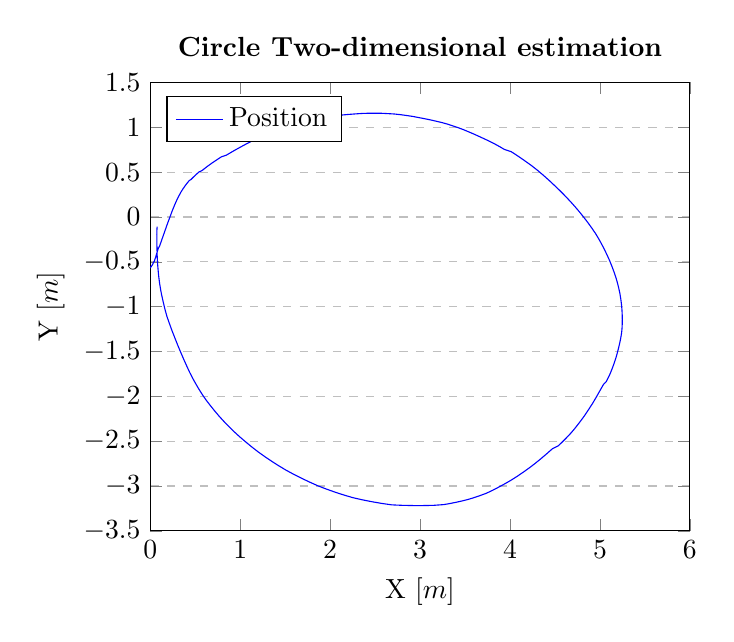
\begin{tikzpicture}
\begin{axis}[
    title={\textbf{Circle Two-dimensional estimation}},
    xlabel={X [$m$]},
    ylabel={Y [$m$]},
    xmin=0, xmax=6,
    ymin=-3.5, ymax=1.5,
    xtick distance = 1,
    ytick distance = 0.5,
    % ytick={-80,-60,-40,-20,0,20,40,60,80,100},
    legend pos=north west,
    ymajorgrids=true,
    grid style=dashed,
]

\addplot[
    color=blue
    ]
    coordinates {(0.07662716,-0.108107)
(0.07660956,-0.1084113)
(0.07656873,-0.1095773)
(0.07642324,-0.1109838)
(0.07627196,-0.1132767)
(0.07603202,-0.1157216)
(0.07586011,-0.1197683)
(0.07562349,-0.1244488)
(0.07533863,-0.1298053)
(0.0749999,-0.1366087)
(0.07456427,-0.140353)
(0.07436436,-0.1453212)
(0.07416244,-0.1511764)
(0.07393353,-0.1586441)
(0.07365805,-0.1672669)
(0.07333251,-0.1760982)
(0.07315216,-0.1855813)
(0.07305408,-0.1907973)
(0.07304657,-0.1936661)
(0.07303401,-0.197026)
(0.07301765,-0.2005236)
(0.0730757,-0.202447)
(0.07312193,-0.2035051)
(0.07313612,-0.2057203)
(0.07317089,-0.2099467)
(0.07326528,-0.2153625)
(0.07343568,-0.2232055)
(0.07366464,-0.2275205)
(0.07372615,-0.2331087)
(0.07373179,-0.2410269)
(0.07373117,-0.2503957)
(0.07366005,-0.2608191)
(0.07373548,-0.2730761)
(0.07379475,-0.2872995)
(0.07403204,-0.3034385)
(0.07448461,-0.3205001)
(0.07482498,-0.3390761)
(0.0752877,-0.3600291)
(0.07580763,-0.3823393)
(0.07633146,-0.4069135)
(0.07731464,-0.4325357)
(0.07843777,-0.4601744)
(0.07989185,-0.4898465)
(0.08192864,-0.5202401)
(0.08433596,-0.5523596)
(0.08722775,-0.5868368)
(0.09044602,-0.6229177)
(0.09421119,-0.6603374)
(0.09875019,-0.6984713)
(0.1041681,-0.7385625)
(0.1106348,-0.7805851)
(0.118054,-0.8239659)
(0.1263697,-0.8672415)
(0.1363633,-0.9125416)
(0.1471304,-0.9594181)
(0.1586013,-1.008416)
(0.1715118,-1.058099)
(0.1850643,-1.10681)
(0.2024605,-1.157679)
(0.221125,-1.209843)
(0.2406909,-1.264103)
(0.2619179,-1.318462)
(0.2834309,-1.373178)
(0.30566,-1.429874)
(0.3296861,-1.487406)
(0.3542998,-1.545394)
(0.3800627,-1.605037)
(0.407619,-1.665809)
(0.436081,-1.728018)
(0.4671623,-1.789507)
(0.5008142,-1.850957)
(0.537158,-1.913476)
(0.5762541,-1.976411)
(0.6171224,-2.036028)
(0.6631914,-2.096457)
(0.7116419,-2.157104)
(0.7623017,-2.217552)
(0.8160631,-2.276937)
(0.8726172,-2.33577)
(0.9323359,-2.394639)
(0.9946569,-2.451505)
(1.059898,-2.507555)
(1.127554,-2.56333)
(1.198306,-2.618646)
(1.271158,-2.670872)
(1.347319,-2.722631)
(1.42589,-2.77311)
(1.507696,-2.822437)
(1.592196,-2.868256)
(1.67923,-2.912273)
(1.768829,-2.955202)
(1.861293,-2.997038)
(1.955817,-3.033605)
(2.05313,-3.068349)
(2.152906,-3.100941)
(2.255443,-3.131082)
(2.360204,-3.154963)
(2.466835,-3.175981)
(2.575584,-3.194788)
(2.686301,-3.210795)
(2.798938,-3.215762)
(2.912845,-3.218381)
(3.028352,-3.218565)
(3.145621,-3.21632)
(3.264541,-3.207716)
(3.329391,-3.196256)
(3.394907,-3.183249)
(3.462255,-3.16833)
(3.53055,-3.151294)
(3.599583,-3.130409)
(3.66772,-3.106981)
(3.737081,-3.081234)
(3.806559,-3.048624)
(3.873308,-3.013436)
(3.940876,-2.976636)
(4.009054,-2.937364)
(4.077008,-2.894308)
(4.143569,-2.848967)
(4.210625,-2.801241)
(4.277543,-2.749965)
(4.342277,-2.697098)
(4.407299,-2.641667)
(4.472189,-2.584271)
(4.53702,-2.55224)
(4.572261,-2.518155)
(4.607611,-2.483011)
(4.643559,-2.446149)
(4.679944,-2.407001)
(4.71449,-2.36624)
(4.748374,-2.32338)
(4.782344,-2.278865)
(4.816252,-2.233293)
(4.848984,-2.18529)
(4.88132,-2.135965)
(4.914375,-2.085248)
(4.945717,-2.032486)
(4.976836,-1.977889)
(5.008122,-1.922586)
(5.040332,-1.865756)
(5.071874,-1.834068)
(5.088422,-1.800541)
(5.105393,-1.76571)
(5.12057,-1.730272)
(5.135157,-1.693201)
(5.1496,-1.654162)
(5.163756,-1.613869)
(5.177376,-1.571806)
(5.189827,-1.528518)
(5.201273,-1.484588)
(5.212457,-1.438933)
(5.222908,-1.392539)
(5.23235,-1.34398)
(5.240701,-1.294637)
(5.245469,-1.244452)
(5.247941,-1.192305)
(5.248707,-1.139068)
(5.247317,-1.084164)
(5.244347,-1.0279)
(5.238964,-0.9707192)
(5.231486,-0.9120213)
(5.221944,-0.8535369)
(5.209303,-0.794409)
(5.194291,-0.7342177)
(5.177199,-0.6740279)
(5.156901,-0.6143559)
(5.134539,-0.5537327)
(5.110198,-0.4927652)
(5.082835,-0.431181)
(5.053397,-0.3695128)
(5.021775,-0.3077244)
(4.987321,-0.2453778)
(4.951046,-0.1846638)
(4.911,-0.1251508)
(4.867736,-0.06523223)
(4.822526,-0.005755723)
(4.774201,0.05426444)
(4.724144,0.1138004)
(4.671526,0.1725631)
(4.616001,0.2318151)
(4.558981,0.2897236)
(4.498603,0.3480763)
(4.436442,0.4066862)
(4.372825,0.463648)
(4.305521,0.5209744)
(4.237096,0.5746261)
(4.165408,0.6261699)
(4.090852,0.6777675)
(4.014843,0.7276353)
(3.935884,0.7540173)
(3.891813,0.7806587)
(3.846424,0.8057615)
(3.798686,0.8311258)
(3.749575,0.8550473)
(3.699331,0.8786186)
(3.647463,0.9026836)
(3.593905,0.9267319)
(3.539005,0.9500934)
(3.482414,0.9742219)
(3.424575,0.9957422)
(3.365471,1.015584)
(3.30478,1.035771)
(3.242701,1.053099)
(3.179633,1.06805)
(3.115808,1.082713)
(3.051002,1.096072)
(2.98486,1.108828)
(2.918196,1.121696)
(2.850784,1.131599)
(2.782135,1.141264)
(2.712239,1.148715)
(2.641447,1.152923)
(2.57024,1.156672)
(2.498392,1.157532)
(2.425512,1.157072)
(2.351872,1.154508)
(2.277942,1.149495)
(2.203881,1.143693)
(2.128648,1.136986)
(2.052341,1.132363)
(2.010464,1.127138)
(1.967562,1.121507)
(1.92311,1.115242)
(1.878221,1.107355)
(1.833096,1.09974)
(1.787669,1.090071)
(1.742159,1.080105)
(1.695201,1.067862)
(1.648573,1.055031)
(1.601804,1.041178)
(1.554641,1.026056)
(1.507126,1.009732)
(1.458304,0.9926085)
(1.409505,0.9744974)
(1.3601,0.9548919)
(1.309307,0.9338505)
(1.258797,0.9109902)
(1.208673,0.8869772)
(1.1585,0.8616863)
(1.107463,0.8351527)
(1.05518,0.8078062)
(1.003033,0.7796382)
(0.9504426,0.7502485)
(0.8975361,0.7198931)
(0.8444506,0.6883921)
(0.7905004,0.6703982)
(0.7612283,0.6515056)
(0.7308221,0.6314625)
(0.7002898,0.6108932)
(0.6692417,0.5891349)
(0.63744,0.565975)
(0.606451,0.5421044)
(0.5748828,0.5168479)
(0.5434113,0.5029204)
(0.5261312,0.4879585)
(0.5084058,0.4720339)
(0.4904602,0.4548357)
(0.471645,0.4366344)
(0.4530249,0.417759)
(0.4346954,0.4070539)
(0.4249586,0.3956739)
(0.415203,0.3835817)
(0.405044,0.3707895)
(0.3946357,0.3573316)
(0.3842826,0.3428377)
(0.373556,0.3272349)
(0.3623665,0.3109932)
(0.351321,0.293727)
(0.3400751,0.2754713)
(0.3293846,0.2553326)
(0.3179113,0.2340052)
(0.3067189,0.2117267)
(0.2956013,0.1889337)
(0.2848861,0.1650812)
(0.2739808,0.1399775)
(0.262928,0.1137024)
(0.2517387,0.08675259)
(0.2408714,0.05854091)
(0.2300029,0.02900109)
(0.2185732,-0.001593633)
(0.2068445,-0.03338885)
(0.1948524,-0.06549362)
(0.1827649,-0.09938616)
(0.1704985,-0.1347195)
(0.1575918,-0.1713076)
(0.1444609,-0.2089541)
(0.130826,-0.2470724)
(0.1173113,-0.286344)
(0.1037257,-0.3259525)
(0.09047795,-0.3478062)
(0.08340144,-0.3701706)
(0.07624226,-0.3936564)
(0.06904179,-0.4181252)
(0.06154352,-0.4433205)
(0.05378386,-0.4685158)
(0.04526258,-0.493571)
(0.03593686,-0.5071532)
(0.03030384,-0.5207251)
(0.02423049,-0.5344185)
(0.01786181,-0.5418604)
(0.01417285,-0.549336)
(0.01025013,-0.5534008)
(0.008005803,-0.555619)
(0.006740261,-0.556838)
(0.006042591,-0.5582869)
(0.00520472,-0.5590827)
(0.004742183,-0.5600827)
(0.004161281,-0.5612433)
(0.003492399,-0.5625775)
(0.002734684,-0.5640638)
(0.001869893,-0.5648782)
(0.001388817,-0.5653265)
(0.001125028,-0.5655728)
(0.0009794129,-0.5657071)
(0.0008973733,-0.5657804)
(0.0008512991,-0.5658207)
(0.0008261612,-0.565843)
(0.0008123057,-0.5658552)
(0.0008046668,-0.5658619)
(0.0008004358,-0.5658656)
(0.0007980942,-0.5658676)
(0.0007967926,-0.5658687)
(0.0007960635,-0.5658693)
(0.0007956676,-0.5658696)
(0.0007954495,-0.5658698)
};
    \addlegendentry{Position }

\end{axis}
\end{tikzpicture}
    \caption{Same experiment conducted in figure \ref{fig:2dimension}  with Z-axis altitude estimation. }
    \label{fig:3dimensions}
\end{figure}


\begin{figure}[!h]
    %% Creator: Matplotlib, PGF backend
%%
%% To include the figure in your LaTeX document, write
%%   \input{<filename>.pgf}
%%
%% Make sure the required packages are loaded in your preamble
%%   \usepackage{pgf}
%%
%% and, on pdftex
%%   \usepackage[utf8]{inputenc}\DeclareUnicodeCharacter{2212}{-}
%%
%% or, on luatex and xetex
%%   \usepackage{unicode-math}
%%
%% Figures using additional raster images can only be included by \input if
%% they are in the same directory as the main LaTeX file. For loading figures
%% from other directories you can use the `import` package
%%   \usepackage{import}
%%
%% and then include the figures with
%%   \import{<path to file>}{<filename>.pgf}
%%
%% Matplotlib used the following preamble
%%   \usepackage{fontspec}
%%
\begingroup%
\makeatletter%
\begin{pgfpicture}%
\pgfpathrectangle{\pgfpointorigin}{\pgfqpoint{5.629167in}{4.311000in}}%
\pgfusepath{use as bounding box, clip}%
\begin{pgfscope}%
\pgfsetbuttcap%
\pgfsetmiterjoin%
\definecolor{currentfill}{rgb}{1.000000,1.000000,1.000000}%
\pgfsetfillcolor{currentfill}%
\pgfsetlinewidth{0.000000pt}%
\definecolor{currentstroke}{rgb}{1.000000,1.000000,1.000000}%
\pgfsetstrokecolor{currentstroke}%
\pgfsetdash{}{0pt}%
\pgfpathmoveto{\pgfqpoint{0.000000in}{0.000000in}}%
\pgfpathlineto{\pgfqpoint{5.629167in}{0.000000in}}%
\pgfpathlineto{\pgfqpoint{5.629167in}{4.311000in}}%
\pgfpathlineto{\pgfqpoint{0.000000in}{4.311000in}}%
\pgfpathclose%
\pgfusepath{fill}%
\end{pgfscope}%
\begin{pgfscope}%
\pgfsetbuttcap%
\pgfsetmiterjoin%
\definecolor{currentfill}{rgb}{1.000000,1.000000,1.000000}%
\pgfsetfillcolor{currentfill}%
\pgfsetlinewidth{0.000000pt}%
\definecolor{currentstroke}{rgb}{0.000000,0.000000,0.000000}%
\pgfsetstrokecolor{currentstroke}%
\pgfsetstrokeopacity{0.000000}%
\pgfsetdash{}{0pt}%
\pgfpathmoveto{\pgfqpoint{0.569167in}{0.515000in}}%
\pgfpathlineto{\pgfqpoint{5.529167in}{0.515000in}}%
\pgfpathlineto{\pgfqpoint{5.529167in}{4.211000in}}%
\pgfpathlineto{\pgfqpoint{0.569167in}{4.211000in}}%
\pgfpathclose%
\pgfusepath{fill}%
\end{pgfscope}%
\begin{pgfscope}%
\pgfpathrectangle{\pgfqpoint{0.569167in}{0.515000in}}{\pgfqpoint{4.960000in}{3.696000in}}%
\pgfusepath{clip}%
\pgfsetbuttcap%
\pgfsetroundjoin%
\definecolor{currentfill}{rgb}{0.121569,0.466667,0.705882}%
\pgfsetfillcolor{currentfill}%
\pgfsetlinewidth{1.003750pt}%
\definecolor{currentstroke}{rgb}{0.121569,0.466667,0.705882}%
\pgfsetstrokecolor{currentstroke}%
\pgfsetdash{}{0pt}%
\pgfsys@defobject{currentmarker}{\pgfqpoint{-0.041667in}{-0.041667in}}{\pgfqpoint{0.041667in}{0.041667in}}{%
\pgfpathmoveto{\pgfqpoint{0.000000in}{-0.041667in}}%
\pgfpathcurveto{\pgfqpoint{0.011050in}{-0.041667in}}{\pgfqpoint{0.021649in}{-0.037276in}}{\pgfqpoint{0.029463in}{-0.029463in}}%
\pgfpathcurveto{\pgfqpoint{0.037276in}{-0.021649in}}{\pgfqpoint{0.041667in}{-0.011050in}}{\pgfqpoint{0.041667in}{0.000000in}}%
\pgfpathcurveto{\pgfqpoint{0.041667in}{0.011050in}}{\pgfqpoint{0.037276in}{0.021649in}}{\pgfqpoint{0.029463in}{0.029463in}}%
\pgfpathcurveto{\pgfqpoint{0.021649in}{0.037276in}}{\pgfqpoint{0.011050in}{0.041667in}}{\pgfqpoint{0.000000in}{0.041667in}}%
\pgfpathcurveto{\pgfqpoint{-0.011050in}{0.041667in}}{\pgfqpoint{-0.021649in}{0.037276in}}{\pgfqpoint{-0.029463in}{0.029463in}}%
\pgfpathcurveto{\pgfqpoint{-0.037276in}{0.021649in}}{\pgfqpoint{-0.041667in}{0.011050in}}{\pgfqpoint{-0.041667in}{0.000000in}}%
\pgfpathcurveto{\pgfqpoint{-0.041667in}{-0.011050in}}{\pgfqpoint{-0.037276in}{-0.021649in}}{\pgfqpoint{-0.029463in}{-0.029463in}}%
\pgfpathcurveto{\pgfqpoint{-0.021649in}{-0.037276in}}{\pgfqpoint{-0.011050in}{-0.041667in}}{\pgfqpoint{0.000000in}{-0.041667in}}%
\pgfpathclose%
\pgfusepath{stroke,fill}%
}%
\begin{pgfscope}%
\pgfsys@transformshift{1.954384in}{1.552463in}%
\pgfsys@useobject{currentmarker}{}%
\end{pgfscope}%
\begin{pgfscope}%
\pgfsys@transformshift{1.964633in}{1.540951in}%
\pgfsys@useobject{currentmarker}{}%
\end{pgfscope}%
\begin{pgfscope}%
\pgfsys@transformshift{1.972214in}{1.518795in}%
\pgfsys@useobject{currentmarker}{}%
\end{pgfscope}%
\begin{pgfscope}%
\pgfsys@transformshift{1.974535in}{1.488206in}%
\pgfsys@useobject{currentmarker}{}%
\end{pgfscope}%
\begin{pgfscope}%
\pgfsys@transformshift{1.975147in}{1.451454in}%
\pgfsys@useobject{currentmarker}{}%
\end{pgfscope}%
\begin{pgfscope}%
\pgfsys@transformshift{1.974234in}{1.411278in}%
\pgfsys@useobject{currentmarker}{}%
\end{pgfscope}%
\begin{pgfscope}%
\pgfsys@transformshift{1.973417in}{1.389185in}%
\pgfsys@useobject{currentmarker}{}%
\end{pgfscope}%
\begin{pgfscope}%
\pgfsys@transformshift{1.973661in}{1.377032in}%
\pgfsys@useobject{currentmarker}{}%
\end{pgfscope}%
\begin{pgfscope}%
\pgfsys@transformshift{1.973382in}{1.370349in}%
\pgfsys@useobject{currentmarker}{}%
\end{pgfscope}%
\begin{pgfscope}%
\pgfsys@transformshift{1.973207in}{1.366674in}%
\pgfsys@useobject{currentmarker}{}%
\end{pgfscope}%
\begin{pgfscope}%
\pgfsys@transformshift{1.973142in}{1.364652in}%
\pgfsys@useobject{currentmarker}{}%
\end{pgfscope}%
\begin{pgfscope}%
\pgfsys@transformshift{1.973004in}{1.363544in}%
\pgfsys@useobject{currentmarker}{}%
\end{pgfscope}%
\begin{pgfscope}%
\pgfsys@transformshift{1.972947in}{1.362933in}%
\pgfsys@useobject{currentmarker}{}%
\end{pgfscope}%
\begin{pgfscope}%
\pgfsys@transformshift{1.972934in}{1.362597in}%
\pgfsys@useobject{currentmarker}{}%
\end{pgfscope}%
\begin{pgfscope}%
\pgfsys@transformshift{1.972927in}{1.362412in}%
\pgfsys@useobject{currentmarker}{}%
\end{pgfscope}%
\begin{pgfscope}%
\pgfsys@transformshift{1.972918in}{1.362310in}%
\pgfsys@useobject{currentmarker}{}%
\end{pgfscope}%
\begin{pgfscope}%
\pgfsys@transformshift{1.972914in}{1.362254in}%
\pgfsys@useobject{currentmarker}{}%
\end{pgfscope}%
\begin{pgfscope}%
\pgfsys@transformshift{1.972913in}{1.362223in}%
\pgfsys@useobject{currentmarker}{}%
\end{pgfscope}%
\begin{pgfscope}%
\pgfsys@transformshift{1.972912in}{1.362206in}%
\pgfsys@useobject{currentmarker}{}%
\end{pgfscope}%
\begin{pgfscope}%
\pgfsys@transformshift{1.972911in}{1.362197in}%
\pgfsys@useobject{currentmarker}{}%
\end{pgfscope}%
\begin{pgfscope}%
\pgfsys@transformshift{1.972911in}{1.362192in}%
\pgfsys@useobject{currentmarker}{}%
\end{pgfscope}%
\begin{pgfscope}%
\pgfsys@transformshift{1.972911in}{1.362189in}%
\pgfsys@useobject{currentmarker}{}%
\end{pgfscope}%
\begin{pgfscope}%
\pgfsys@transformshift{1.972709in}{1.359295in}%
\pgfsys@useobject{currentmarker}{}%
\end{pgfscope}%
\begin{pgfscope}%
\pgfsys@transformshift{1.972657in}{1.357703in}%
\pgfsys@useobject{currentmarker}{}%
\end{pgfscope}%
\begin{pgfscope}%
\pgfsys@transformshift{1.972601in}{1.356827in}%
\pgfsys@useobject{currentmarker}{}%
\end{pgfscope}%
\begin{pgfscope}%
\pgfsys@transformshift{1.972548in}{1.356346in}%
\pgfsys@useobject{currentmarker}{}%
\end{pgfscope}%
\begin{pgfscope}%
\pgfsys@transformshift{1.972530in}{1.356082in}%
\pgfsys@useobject{currentmarker}{}%
\end{pgfscope}%
\begin{pgfscope}%
\pgfsys@transformshift{1.972517in}{1.355936in}%
\pgfsys@useobject{currentmarker}{}%
\end{pgfscope}%
\begin{pgfscope}%
\pgfsys@transformshift{1.972511in}{1.355856in}%
\pgfsys@useobject{currentmarker}{}%
\end{pgfscope}%
\begin{pgfscope}%
\pgfsys@transformshift{1.972509in}{1.355812in}%
\pgfsys@useobject{currentmarker}{}%
\end{pgfscope}%
\begin{pgfscope}%
\pgfsys@transformshift{1.972506in}{1.355788in}%
\pgfsys@useobject{currentmarker}{}%
\end{pgfscope}%
\begin{pgfscope}%
\pgfsys@transformshift{1.972136in}{1.352682in}%
\pgfsys@useobject{currentmarker}{}%
\end{pgfscope}%
\begin{pgfscope}%
\pgfsys@transformshift{1.971822in}{1.350981in}%
\pgfsys@useobject{currentmarker}{}%
\end{pgfscope}%
\begin{pgfscope}%
\pgfsys@transformshift{1.971577in}{1.350052in}%
\pgfsys@useobject{currentmarker}{}%
\end{pgfscope}%
\begin{pgfscope}%
\pgfsys@transformshift{1.971419in}{1.349543in}%
\pgfsys@useobject{currentmarker}{}%
\end{pgfscope}%
\begin{pgfscope}%
\pgfsys@transformshift{1.971284in}{1.349271in}%
\pgfsys@useobject{currentmarker}{}%
\end{pgfscope}%
\begin{pgfscope}%
\pgfsys@transformshift{1.971175in}{1.349131in}%
\pgfsys@useobject{currentmarker}{}%
\end{pgfscope}%
\begin{pgfscope}%
\pgfsys@transformshift{1.971093in}{1.349062in}%
\pgfsys@useobject{currentmarker}{}%
\end{pgfscope}%
\begin{pgfscope}%
\pgfsys@transformshift{1.971035in}{1.349032in}%
\pgfsys@useobject{currentmarker}{}%
\end{pgfscope}%
\begin{pgfscope}%
\pgfsys@transformshift{1.962992in}{1.346171in}%
\pgfsys@useobject{currentmarker}{}%
\end{pgfscope}%
\begin{pgfscope}%
\pgfsys@transformshift{1.958251in}{1.345026in}%
\pgfsys@useobject{currentmarker}{}%
\end{pgfscope}%
\begin{pgfscope}%
\pgfsys@transformshift{1.947932in}{1.343822in}%
\pgfsys@useobject{currentmarker}{}%
\end{pgfscope}%
\begin{pgfscope}%
\pgfsys@transformshift{1.926441in}{1.343800in}%
\pgfsys@useobject{currentmarker}{}%
\end{pgfscope}%
\begin{pgfscope}%
\pgfsys@transformshift{1.914806in}{1.345118in}%
\pgfsys@useobject{currentmarker}{}%
\end{pgfscope}%
\begin{pgfscope}%
\pgfsys@transformshift{1.908752in}{1.346619in}%
\pgfsys@useobject{currentmarker}{}%
\end{pgfscope}%
\begin{pgfscope}%
\pgfsys@transformshift{1.882841in}{1.356417in}%
\pgfsys@useobject{currentmarker}{}%
\end{pgfscope}%
\begin{pgfscope}%
\pgfsys@transformshift{1.855403in}{1.371038in}%
\pgfsys@useobject{currentmarker}{}%
\end{pgfscope}%
\begin{pgfscope}%
\pgfsys@transformshift{1.826478in}{1.392768in}%
\pgfsys@useobject{currentmarker}{}%
\end{pgfscope}%
\begin{pgfscope}%
\pgfsys@transformshift{1.797393in}{1.422835in}%
\pgfsys@useobject{currentmarker}{}%
\end{pgfscope}%
\begin{pgfscope}%
\pgfsys@transformshift{1.767396in}{1.462303in}%
\pgfsys@useobject{currentmarker}{}%
\end{pgfscope}%
\begin{pgfscope}%
\pgfsys@transformshift{1.754743in}{1.485021in}%
\pgfsys@useobject{currentmarker}{}%
\end{pgfscope}%
\begin{pgfscope}%
\pgfsys@transformshift{1.741971in}{1.515298in}%
\pgfsys@useobject{currentmarker}{}%
\end{pgfscope}%
\begin{pgfscope}%
\pgfsys@transformshift{1.737174in}{1.532265in}%
\pgfsys@useobject{currentmarker}{}%
\end{pgfscope}%
\begin{pgfscope}%
\pgfsys@transformshift{1.733552in}{1.552749in}%
\pgfsys@useobject{currentmarker}{}%
\end{pgfscope}%
\begin{pgfscope}%
\pgfsys@transformshift{1.730853in}{1.576080in}%
\pgfsys@useobject{currentmarker}{}%
\end{pgfscope}%
\begin{pgfscope}%
\pgfsys@transformshift{1.729674in}{1.588925in}%
\pgfsys@useobject{currentmarker}{}%
\end{pgfscope}%
\begin{pgfscope}%
\pgfsys@transformshift{1.729221in}{1.595996in}%
\pgfsys@useobject{currentmarker}{}%
\end{pgfscope}%
\begin{pgfscope}%
\pgfsys@transformshift{1.728969in}{1.599885in}%
\pgfsys@useobject{currentmarker}{}%
\end{pgfscope}%
\begin{pgfscope}%
\pgfsys@transformshift{1.728848in}{1.602024in}%
\pgfsys@useobject{currentmarker}{}%
\end{pgfscope}%
\begin{pgfscope}%
\pgfsys@transformshift{1.728832in}{1.603201in}%
\pgfsys@useobject{currentmarker}{}%
\end{pgfscope}%
\begin{pgfscope}%
\pgfsys@transformshift{1.728624in}{1.607224in}%
\pgfsys@useobject{currentmarker}{}%
\end{pgfscope}%
\begin{pgfscope}%
\pgfsys@transformshift{1.728534in}{1.609436in}%
\pgfsys@useobject{currentmarker}{}%
\end{pgfscope}%
\begin{pgfscope}%
\pgfsys@transformshift{1.728431in}{1.610654in}%
\pgfsys@useobject{currentmarker}{}%
\end{pgfscope}%
\begin{pgfscope}%
\pgfsys@transformshift{1.728356in}{1.611321in}%
\pgfsys@useobject{currentmarker}{}%
\end{pgfscope}%
\begin{pgfscope}%
\pgfsys@transformshift{1.728318in}{1.611689in}%
\pgfsys@useobject{currentmarker}{}%
\end{pgfscope}%
\begin{pgfscope}%
\pgfsys@transformshift{1.727882in}{1.616237in}%
\pgfsys@useobject{currentmarker}{}%
\end{pgfscope}%
\begin{pgfscope}%
\pgfsys@transformshift{1.727679in}{1.618739in}%
\pgfsys@useobject{currentmarker}{}%
\end{pgfscope}%
\begin{pgfscope}%
\pgfsys@transformshift{1.727597in}{1.620116in}%
\pgfsys@useobject{currentmarker}{}%
\end{pgfscope}%
\begin{pgfscope}%
\pgfsys@transformshift{1.727038in}{1.624850in}%
\pgfsys@useobject{currentmarker}{}%
\end{pgfscope}%
\begin{pgfscope}%
\pgfsys@transformshift{1.726499in}{1.632817in}%
\pgfsys@useobject{currentmarker}{}%
\end{pgfscope}%
\begin{pgfscope}%
\pgfsys@transformshift{1.721658in}{1.655945in}%
\pgfsys@useobject{currentmarker}{}%
\end{pgfscope}%
\begin{pgfscope}%
\pgfsys@transformshift{1.721117in}{1.668772in}%
\pgfsys@useobject{currentmarker}{}%
\end{pgfscope}%
\begin{pgfscope}%
\pgfsys@transformshift{1.719736in}{1.675775in}%
\pgfsys@useobject{currentmarker}{}%
\end{pgfscope}%
\begin{pgfscope}%
\pgfsys@transformshift{1.717738in}{1.698901in}%
\pgfsys@useobject{currentmarker}{}%
\end{pgfscope}%
\begin{pgfscope}%
\pgfsys@transformshift{1.710507in}{1.730630in}%
\pgfsys@useobject{currentmarker}{}%
\end{pgfscope}%
\begin{pgfscope}%
\pgfsys@transformshift{1.703909in}{1.781218in}%
\pgfsys@useobject{currentmarker}{}%
\end{pgfscope}%
\begin{pgfscope}%
\pgfsys@transformshift{1.691740in}{1.841359in}%
\pgfsys@useobject{currentmarker}{}%
\end{pgfscope}%
\begin{pgfscope}%
\pgfsys@transformshift{1.688320in}{1.874637in}%
\pgfsys@useobject{currentmarker}{}%
\end{pgfscope}%
\begin{pgfscope}%
\pgfsys@transformshift{1.684872in}{1.892848in}%
\pgfsys@useobject{currentmarker}{}%
\end{pgfscope}%
\begin{pgfscope}%
\pgfsys@transformshift{1.685224in}{1.914305in}%
\pgfsys@useobject{currentmarker}{}%
\end{pgfscope}%
\begin{pgfscope}%
\pgfsys@transformshift{1.681895in}{1.939483in}%
\pgfsys@useobject{currentmarker}{}%
\end{pgfscope}%
\begin{pgfscope}%
\pgfsys@transformshift{1.682800in}{1.953367in}%
\pgfsys@useobject{currentmarker}{}%
\end{pgfscope}%
\begin{pgfscope}%
\pgfsys@transformshift{1.680775in}{1.973941in}%
\pgfsys@useobject{currentmarker}{}%
\end{pgfscope}%
\begin{pgfscope}%
\pgfsys@transformshift{1.683217in}{1.998952in}%
\pgfsys@useobject{currentmarker}{}%
\end{pgfscope}%
\begin{pgfscope}%
\pgfsys@transformshift{1.681508in}{2.029666in}%
\pgfsys@useobject{currentmarker}{}%
\end{pgfscope}%
\begin{pgfscope}%
\pgfsys@transformshift{1.686180in}{2.066188in}%
\pgfsys@useobject{currentmarker}{}%
\end{pgfscope}%
\begin{pgfscope}%
\pgfsys@transformshift{1.685492in}{2.107361in}%
\pgfsys@useobject{currentmarker}{}%
\end{pgfscope}%
\begin{pgfscope}%
\pgfsys@transformshift{1.688268in}{2.159246in}%
\pgfsys@useobject{currentmarker}{}%
\end{pgfscope}%
\begin{pgfscope}%
\pgfsys@transformshift{1.681342in}{2.218445in}%
\pgfsys@useobject{currentmarker}{}%
\end{pgfscope}%
\begin{pgfscope}%
\pgfsys@transformshift{1.681527in}{2.250986in}%
\pgfsys@useobject{currentmarker}{}%
\end{pgfscope}%
\begin{pgfscope}%
\pgfsys@transformshift{1.674229in}{2.288586in}%
\pgfsys@useobject{currentmarker}{}%
\end{pgfscope}%
\begin{pgfscope}%
\pgfsys@transformshift{1.673636in}{2.309414in}%
\pgfsys@useobject{currentmarker}{}%
\end{pgfscope}%
\begin{pgfscope}%
\pgfsys@transformshift{1.671319in}{2.320760in}%
\pgfsys@useobject{currentmarker}{}%
\end{pgfscope}%
\begin{pgfscope}%
\pgfsys@transformshift{1.670457in}{2.340989in}%
\pgfsys@useobject{currentmarker}{}%
\end{pgfscope}%
\begin{pgfscope}%
\pgfsys@transformshift{1.663921in}{2.370925in}%
\pgfsys@useobject{currentmarker}{}%
\end{pgfscope}%
\begin{pgfscope}%
\pgfsys@transformshift{1.660349in}{2.409444in}%
\pgfsys@useobject{currentmarker}{}%
\end{pgfscope}%
\begin{pgfscope}%
\pgfsys@transformshift{1.648015in}{2.455356in}%
\pgfsys@useobject{currentmarker}{}%
\end{pgfscope}%
\begin{pgfscope}%
\pgfsys@transformshift{1.641185in}{2.511854in}%
\pgfsys@useobject{currentmarker}{}%
\end{pgfscope}%
\begin{pgfscope}%
\pgfsys@transformshift{1.618156in}{2.579926in}%
\pgfsys@useobject{currentmarker}{}%
\end{pgfscope}%
\begin{pgfscope}%
\pgfsys@transformshift{1.603466in}{2.656977in}%
\pgfsys@useobject{currentmarker}{}%
\end{pgfscope}%
\begin{pgfscope}%
\pgfsys@transformshift{1.580629in}{2.745095in}%
\pgfsys@useobject{currentmarker}{}%
\end{pgfscope}%
\begin{pgfscope}%
\pgfsys@transformshift{1.564757in}{2.838781in}%
\pgfsys@useobject{currentmarker}{}%
\end{pgfscope}%
\begin{pgfscope}%
\pgfsys@transformshift{1.537085in}{2.938271in}%
\pgfsys@useobject{currentmarker}{}%
\end{pgfscope}%
\begin{pgfscope}%
\pgfsys@transformshift{1.526553in}{2.993430in}%
\pgfsys@useobject{currentmarker}{}%
\end{pgfscope}%
\begin{pgfscope}%
\pgfsys@transformshift{1.512642in}{3.051347in}%
\pgfsys@useobject{currentmarker}{}%
\end{pgfscope}%
\begin{pgfscope}%
\pgfsys@transformshift{1.506035in}{3.083295in}%
\pgfsys@useobject{currentmarker}{}%
\end{pgfscope}%
\begin{pgfscope}%
\pgfsys@transformshift{1.496761in}{3.121193in}%
\pgfsys@useobject{currentmarker}{}%
\end{pgfscope}%
\begin{pgfscope}%
\pgfsys@transformshift{1.492038in}{3.142073in}%
\pgfsys@useobject{currentmarker}{}%
\end{pgfscope}%
\begin{pgfscope}%
\pgfsys@transformshift{1.485472in}{3.168035in}%
\pgfsys@useobject{currentmarker}{}%
\end{pgfscope}%
\begin{pgfscope}%
\pgfsys@transformshift{1.482705in}{3.182390in}%
\pgfsys@useobject{currentmarker}{}%
\end{pgfscope}%
\begin{pgfscope}%
\pgfsys@transformshift{1.480476in}{3.190217in}%
\pgfsys@useobject{currentmarker}{}%
\end{pgfscope}%
\begin{pgfscope}%
\pgfsys@transformshift{1.479671in}{3.194562in}%
\pgfsys@useobject{currentmarker}{}%
\end{pgfscope}%
\begin{pgfscope}%
\pgfsys@transformshift{1.477623in}{3.202275in}%
\pgfsys@useobject{currentmarker}{}%
\end{pgfscope}%
\begin{pgfscope}%
\pgfsys@transformshift{1.476780in}{3.206543in}%
\pgfsys@useobject{currentmarker}{}%
\end{pgfscope}%
\begin{pgfscope}%
\pgfsys@transformshift{1.474679in}{3.214601in}%
\pgfsys@useobject{currentmarker}{}%
\end{pgfscope}%
\begin{pgfscope}%
\pgfsys@transformshift{1.473931in}{3.219068in}%
\pgfsys@useobject{currentmarker}{}%
\end{pgfscope}%
\begin{pgfscope}%
\pgfsys@transformshift{1.471971in}{3.226443in}%
\pgfsys@useobject{currentmarker}{}%
\end{pgfscope}%
\begin{pgfscope}%
\pgfsys@transformshift{1.471379in}{3.236773in}%
\pgfsys@useobject{currentmarker}{}%
\end{pgfscope}%
\begin{pgfscope}%
\pgfsys@transformshift{1.468019in}{3.251733in}%
\pgfsys@useobject{currentmarker}{}%
\end{pgfscope}%
\begin{pgfscope}%
\pgfsys@transformshift{1.465989in}{3.259943in}%
\pgfsys@useobject{currentmarker}{}%
\end{pgfscope}%
\begin{pgfscope}%
\pgfsys@transformshift{1.462899in}{3.272473in}%
\pgfsys@useobject{currentmarker}{}%
\end{pgfscope}%
\begin{pgfscope}%
\pgfsys@transformshift{1.458472in}{3.288553in}%
\pgfsys@useobject{currentmarker}{}%
\end{pgfscope}%
\begin{pgfscope}%
\pgfsys@transformshift{1.456417in}{3.297435in}%
\pgfsys@useobject{currentmarker}{}%
\end{pgfscope}%
\begin{pgfscope}%
\pgfsys@transformshift{1.455182in}{3.302310in}%
\pgfsys@useobject{currentmarker}{}%
\end{pgfscope}%
\begin{pgfscope}%
\pgfsys@transformshift{1.454707in}{3.305009in}%
\pgfsys@useobject{currentmarker}{}%
\end{pgfscope}%
\begin{pgfscope}%
\pgfsys@transformshift{1.454337in}{3.306484in}%
\pgfsys@useobject{currentmarker}{}%
\end{pgfscope}%
\begin{pgfscope}%
\pgfsys@transformshift{1.454174in}{3.307299in}%
\pgfsys@useobject{currentmarker}{}%
\end{pgfscope}%
\begin{pgfscope}%
\pgfsys@transformshift{1.452865in}{3.312317in}%
\pgfsys@useobject{currentmarker}{}%
\end{pgfscope}%
\begin{pgfscope}%
\pgfsys@transformshift{1.452337in}{3.315094in}%
\pgfsys@useobject{currentmarker}{}%
\end{pgfscope}%
\begin{pgfscope}%
\pgfsys@transformshift{1.451951in}{3.316613in}%
\pgfsys@useobject{currentmarker}{}%
\end{pgfscope}%
\begin{pgfscope}%
\pgfsys@transformshift{1.450402in}{3.325225in}%
\pgfsys@useobject{currentmarker}{}%
\end{pgfscope}%
\begin{pgfscope}%
\pgfsys@transformshift{1.449389in}{3.329949in}%
\pgfsys@useobject{currentmarker}{}%
\end{pgfscope}%
\begin{pgfscope}%
\pgfsys@transformshift{1.448704in}{3.332534in}%
\pgfsys@useobject{currentmarker}{}%
\end{pgfscope}%
\begin{pgfscope}%
\pgfsys@transformshift{1.447518in}{3.338206in}%
\pgfsys@useobject{currentmarker}{}%
\end{pgfscope}%
\begin{pgfscope}%
\pgfsys@transformshift{1.444828in}{3.348306in}%
\pgfsys@useobject{currentmarker}{}%
\end{pgfscope}%
\begin{pgfscope}%
\pgfsys@transformshift{1.443699in}{3.353894in}%
\pgfsys@useobject{currentmarker}{}%
\end{pgfscope}%
\begin{pgfscope}%
\pgfsys@transformshift{1.441166in}{3.363498in}%
\pgfsys@useobject{currentmarker}{}%
\end{pgfscope}%
\begin{pgfscope}%
\pgfsys@transformshift{1.440131in}{3.368813in}%
\pgfsys@useobject{currentmarker}{}%
\end{pgfscope}%
\begin{pgfscope}%
\pgfsys@transformshift{1.438330in}{3.378463in}%
\pgfsys@useobject{currentmarker}{}%
\end{pgfscope}%
\begin{pgfscope}%
\pgfsys@transformshift{1.427790in}{3.431211in}%
\pgfsys@useobject{currentmarker}{}%
\end{pgfscope}%
\begin{pgfscope}%
\pgfsys@transformshift{1.421765in}{3.460204in}%
\pgfsys@useobject{currentmarker}{}%
\end{pgfscope}%
\begin{pgfscope}%
\pgfsys@transformshift{1.418477in}{3.476152in}%
\pgfsys@useobject{currentmarker}{}%
\end{pgfscope}%
\begin{pgfscope}%
\pgfsys@transformshift{1.416613in}{3.484919in}%
\pgfsys@useobject{currentmarker}{}%
\end{pgfscope}%
\begin{pgfscope}%
\pgfsys@transformshift{1.415498in}{3.489733in}%
\pgfsys@useobject{currentmarker}{}%
\end{pgfscope}%
\begin{pgfscope}%
\pgfsys@transformshift{1.414946in}{3.492386in}%
\pgfsys@useobject{currentmarker}{}%
\end{pgfscope}%
\begin{pgfscope}%
\pgfsys@transformshift{1.413529in}{3.499723in}%
\pgfsys@useobject{currentmarker}{}%
\end{pgfscope}%
\begin{pgfscope}%
\pgfsys@transformshift{1.413342in}{3.503786in}%
\pgfsys@useobject{currentmarker}{}%
\end{pgfscope}%
\begin{pgfscope}%
\pgfsys@transformshift{1.412525in}{3.513547in}%
\pgfsys@useobject{currentmarker}{}%
\end{pgfscope}%
\begin{pgfscope}%
\pgfsys@transformshift{1.411719in}{3.518899in}%
\pgfsys@useobject{currentmarker}{}%
\end{pgfscope}%
\begin{pgfscope}%
\pgfsys@transformshift{1.411283in}{3.521843in}%
\pgfsys@useobject{currentmarker}{}%
\end{pgfscope}%
\begin{pgfscope}%
\pgfsys@transformshift{1.410975in}{3.523457in}%
\pgfsys@useobject{currentmarker}{}%
\end{pgfscope}%
\begin{pgfscope}%
\pgfsys@transformshift{1.410850in}{3.524348in}%
\pgfsys@useobject{currentmarker}{}%
\end{pgfscope}%
\begin{pgfscope}%
\pgfsys@transformshift{1.410753in}{3.524836in}%
\pgfsys@useobject{currentmarker}{}%
\end{pgfscope}%
\begin{pgfscope}%
\pgfsys@transformshift{1.410712in}{3.525106in}%
\pgfsys@useobject{currentmarker}{}%
\end{pgfscope}%
\begin{pgfscope}%
\pgfsys@transformshift{1.410683in}{3.525253in}%
\pgfsys@useobject{currentmarker}{}%
\end{pgfscope}%
\begin{pgfscope}%
\pgfsys@transformshift{1.408548in}{3.541294in}%
\pgfsys@useobject{currentmarker}{}%
\end{pgfscope}%
\begin{pgfscope}%
\pgfsys@transformshift{1.406512in}{3.550054in}%
\pgfsys@useobject{currentmarker}{}%
\end{pgfscope}%
\begin{pgfscope}%
\pgfsys@transformshift{1.406211in}{3.554920in}%
\pgfsys@useobject{currentmarker}{}%
\end{pgfscope}%
\begin{pgfscope}%
\pgfsys@transformshift{1.404833in}{3.563401in}%
\pgfsys@useobject{currentmarker}{}%
\end{pgfscope}%
\begin{pgfscope}%
\pgfsys@transformshift{1.404183in}{3.568072in}%
\pgfsys@useobject{currentmarker}{}%
\end{pgfscope}%
\begin{pgfscope}%
\pgfsys@transformshift{1.403716in}{3.570634in}%
\pgfsys@useobject{currentmarker}{}%
\end{pgfscope}%
\begin{pgfscope}%
\pgfsys@transformshift{1.401724in}{3.578758in}%
\pgfsys@useobject{currentmarker}{}%
\end{pgfscope}%
\begin{pgfscope}%
\pgfsys@transformshift{1.399969in}{3.590667in}%
\pgfsys@useobject{currentmarker}{}%
\end{pgfscope}%
\begin{pgfscope}%
\pgfsys@transformshift{1.396023in}{3.605358in}%
\pgfsys@useobject{currentmarker}{}%
\end{pgfscope}%
\begin{pgfscope}%
\pgfsys@transformshift{1.393809in}{3.613433in}%
\pgfsys@useobject{currentmarker}{}%
\end{pgfscope}%
\begin{pgfscope}%
\pgfsys@transformshift{1.392585in}{3.617873in}%
\pgfsys@useobject{currentmarker}{}%
\end{pgfscope}%
\begin{pgfscope}%
\pgfsys@transformshift{1.390130in}{3.625277in}%
\pgfsys@useobject{currentmarker}{}%
\end{pgfscope}%
\begin{pgfscope}%
\pgfsys@transformshift{1.388981in}{3.629373in}%
\pgfsys@useobject{currentmarker}{}%
\end{pgfscope}%
\begin{pgfscope}%
\pgfsys@transformshift{1.388078in}{3.631589in}%
\pgfsys@useobject{currentmarker}{}%
\end{pgfscope}%
\begin{pgfscope}%
\pgfsys@transformshift{1.387887in}{3.632842in}%
\pgfsys@useobject{currentmarker}{}%
\end{pgfscope}%
\begin{pgfscope}%
\pgfsys@transformshift{1.387777in}{3.633531in}%
\pgfsys@useobject{currentmarker}{}%
\end{pgfscope}%
\begin{pgfscope}%
\pgfsys@transformshift{1.386283in}{3.638756in}%
\pgfsys@useobject{currentmarker}{}%
\end{pgfscope}%
\begin{pgfscope}%
\pgfsys@transformshift{1.385694in}{3.641652in}%
\pgfsys@useobject{currentmarker}{}%
\end{pgfscope}%
\begin{pgfscope}%
\pgfsys@transformshift{1.383854in}{3.647703in}%
\pgfsys@useobject{currentmarker}{}%
\end{pgfscope}%
\begin{pgfscope}%
\pgfsys@transformshift{1.383690in}{3.651091in}%
\pgfsys@useobject{currentmarker}{}%
\end{pgfscope}%
\begin{pgfscope}%
\pgfsys@transformshift{1.383032in}{3.658824in}%
\pgfsys@useobject{currentmarker}{}%
\end{pgfscope}%
\begin{pgfscope}%
\pgfsys@transformshift{1.380962in}{3.672259in}%
\pgfsys@useobject{currentmarker}{}%
\end{pgfscope}%
\begin{pgfscope}%
\pgfsys@transformshift{1.379866in}{3.679650in}%
\pgfsys@useobject{currentmarker}{}%
\end{pgfscope}%
\begin{pgfscope}%
\pgfsys@transformshift{1.376925in}{3.692527in}%
\pgfsys@useobject{currentmarker}{}%
\end{pgfscope}%
\begin{pgfscope}%
\pgfsys@transformshift{1.375676in}{3.699638in}%
\pgfsys@useobject{currentmarker}{}%
\end{pgfscope}%
\begin{pgfscope}%
\pgfsys@transformshift{1.373061in}{3.711213in}%
\pgfsys@useobject{currentmarker}{}%
\end{pgfscope}%
\begin{pgfscope}%
\pgfsys@transformshift{1.371362in}{3.717553in}%
\pgfsys@useobject{currentmarker}{}%
\end{pgfscope}%
\begin{pgfscope}%
\pgfsys@transformshift{1.370516in}{3.721049in}%
\pgfsys@useobject{currentmarker}{}%
\end{pgfscope}%
\begin{pgfscope}%
\pgfsys@transformshift{1.369992in}{3.722966in}%
\pgfsys@useobject{currentmarker}{}%
\end{pgfscope}%
\begin{pgfscope}%
\pgfsys@transformshift{1.369710in}{3.724021in}%
\pgfsys@useobject{currentmarker}{}%
\end{pgfscope}%
\begin{pgfscope}%
\pgfsys@transformshift{1.368328in}{3.728491in}%
\pgfsys@useobject{currentmarker}{}%
\end{pgfscope}%
\begin{pgfscope}%
\pgfsys@transformshift{1.367571in}{3.730949in}%
\pgfsys@useobject{currentmarker}{}%
\end{pgfscope}%
\begin{pgfscope}%
\pgfsys@transformshift{1.367144in}{3.732300in}%
\pgfsys@useobject{currentmarker}{}%
\end{pgfscope}%
\begin{pgfscope}%
\pgfsys@transformshift{1.365466in}{3.737074in}%
\pgfsys@useobject{currentmarker}{}%
\end{pgfscope}%
\begin{pgfscope}%
\pgfsys@transformshift{1.364713in}{3.739721in}%
\pgfsys@useobject{currentmarker}{}%
\end{pgfscope}%
\begin{pgfscope}%
\pgfsys@transformshift{1.361454in}{3.748065in}%
\pgfsys@useobject{currentmarker}{}%
\end{pgfscope}%
\begin{pgfscope}%
\pgfsys@transformshift{1.359864in}{3.752684in}%
\pgfsys@useobject{currentmarker}{}%
\end{pgfscope}%
\begin{pgfscope}%
\pgfsys@transformshift{1.358983in}{3.755223in}%
\pgfsys@useobject{currentmarker}{}%
\end{pgfscope}%
\begin{pgfscope}%
\pgfsys@transformshift{1.356247in}{3.762428in}%
\pgfsys@useobject{currentmarker}{}%
\end{pgfscope}%
\begin{pgfscope}%
\pgfsys@transformshift{1.354866in}{3.766409in}%
\pgfsys@useobject{currentmarker}{}%
\end{pgfscope}%
\begin{pgfscope}%
\pgfsys@transformshift{1.351272in}{3.776032in}%
\pgfsys@useobject{currentmarker}{}%
\end{pgfscope}%
\begin{pgfscope}%
\pgfsys@transformshift{1.349307in}{3.781326in}%
\pgfsys@useobject{currentmarker}{}%
\end{pgfscope}%
\begin{pgfscope}%
\pgfsys@transformshift{1.348274in}{3.784245in}%
\pgfsys@useobject{currentmarker}{}%
\end{pgfscope}%
\begin{pgfscope}%
\pgfsys@transformshift{1.345645in}{3.790622in}%
\pgfsys@useobject{currentmarker}{}%
\end{pgfscope}%
\begin{pgfscope}%
\pgfsys@transformshift{1.344437in}{3.794165in}%
\pgfsys@useobject{currentmarker}{}%
\end{pgfscope}%
\begin{pgfscope}%
\pgfsys@transformshift{1.341307in}{3.802649in}%
\pgfsys@useobject{currentmarker}{}%
\end{pgfscope}%
\begin{pgfscope}%
\pgfsys@transformshift{1.339772in}{3.807342in}%
\pgfsys@useobject{currentmarker}{}%
\end{pgfscope}%
\begin{pgfscope}%
\pgfsys@transformshift{1.339017in}{3.809934in}%
\pgfsys@useobject{currentmarker}{}%
\end{pgfscope}%
\begin{pgfscope}%
\pgfsys@transformshift{1.336395in}{3.818770in}%
\pgfsys@useobject{currentmarker}{}%
\end{pgfscope}%
\begin{pgfscope}%
\pgfsys@transformshift{1.332952in}{3.830571in}%
\pgfsys@useobject{currentmarker}{}%
\end{pgfscope}%
\begin{pgfscope}%
\pgfsys@transformshift{1.330627in}{3.837005in}%
\pgfsys@useobject{currentmarker}{}%
\end{pgfscope}%
\begin{pgfscope}%
\pgfsys@transformshift{1.329806in}{3.840597in}%
\pgfsys@useobject{currentmarker}{}%
\end{pgfscope}%
\begin{pgfscope}%
\pgfsys@transformshift{1.327107in}{3.850546in}%
\pgfsys@useobject{currentmarker}{}%
\end{pgfscope}%
\begin{pgfscope}%
\pgfsys@transformshift{1.325224in}{3.855968in}%
\pgfsys@useobject{currentmarker}{}%
\end{pgfscope}%
\begin{pgfscope}%
\pgfsys@transformshift{1.323208in}{3.864961in}%
\pgfsys@useobject{currentmarker}{}%
\end{pgfscope}%
\begin{pgfscope}%
\pgfsys@transformshift{1.321585in}{3.869850in}%
\pgfsys@useobject{currentmarker}{}%
\end{pgfscope}%
\begin{pgfscope}%
\pgfsys@transformshift{1.320858in}{3.872558in}%
\pgfsys@useobject{currentmarker}{}%
\end{pgfscope}%
\begin{pgfscope}%
\pgfsys@transformshift{1.318908in}{3.879704in}%
\pgfsys@useobject{currentmarker}{}%
\end{pgfscope}%
\begin{pgfscope}%
\pgfsys@transformshift{1.316628in}{3.889679in}%
\pgfsys@useobject{currentmarker}{}%
\end{pgfscope}%
\begin{pgfscope}%
\pgfsys@transformshift{1.313099in}{3.903532in}%
\pgfsys@useobject{currentmarker}{}%
\end{pgfscope}%
\begin{pgfscope}%
\pgfsys@transformshift{1.310946in}{3.911129in}%
\pgfsys@useobject{currentmarker}{}%
\end{pgfscope}%
\begin{pgfscope}%
\pgfsys@transformshift{1.308132in}{3.921855in}%
\pgfsys@useobject{currentmarker}{}%
\end{pgfscope}%
\begin{pgfscope}%
\pgfsys@transformshift{1.306447in}{3.927739in}%
\pgfsys@useobject{currentmarker}{}%
\end{pgfscope}%
\begin{pgfscope}%
\pgfsys@transformshift{1.304264in}{3.936408in}%
\pgfsys@useobject{currentmarker}{}%
\end{pgfscope}%
\begin{pgfscope}%
\pgfsys@transformshift{1.303054in}{3.941175in}%
\pgfsys@useobject{currentmarker}{}%
\end{pgfscope}%
\begin{pgfscope}%
\pgfsys@transformshift{1.302382in}{3.943796in}%
\pgfsys@useobject{currentmarker}{}%
\end{pgfscope}%
\begin{pgfscope}%
\pgfsys@transformshift{1.302039in}{3.945240in}%
\pgfsys@useobject{currentmarker}{}%
\end{pgfscope}%
\begin{pgfscope}%
\pgfsys@transformshift{1.301838in}{3.946033in}%
\pgfsys@useobject{currentmarker}{}%
\end{pgfscope}%
\begin{pgfscope}%
\pgfsys@transformshift{1.301719in}{3.946469in}%
\pgfsys@useobject{currentmarker}{}%
\end{pgfscope}%
\begin{pgfscope}%
\pgfsys@transformshift{1.301658in}{3.946709in}%
\pgfsys@useobject{currentmarker}{}%
\end{pgfscope}%
\begin{pgfscope}%
\pgfsys@transformshift{1.301626in}{3.946841in}%
\pgfsys@useobject{currentmarker}{}%
\end{pgfscope}%
\begin{pgfscope}%
\pgfsys@transformshift{1.301608in}{3.946913in}%
\pgfsys@useobject{currentmarker}{}%
\end{pgfscope}%
\begin{pgfscope}%
\pgfsys@transformshift{1.301598in}{3.946953in}%
\pgfsys@useobject{currentmarker}{}%
\end{pgfscope}%
\begin{pgfscope}%
\pgfsys@transformshift{1.300634in}{3.950499in}%
\pgfsys@useobject{currentmarker}{}%
\end{pgfscope}%
\begin{pgfscope}%
\pgfsys@transformshift{1.300089in}{3.952448in}%
\pgfsys@useobject{currentmarker}{}%
\end{pgfscope}%
\begin{pgfscope}%
\pgfsys@transformshift{1.298798in}{3.957446in}%
\pgfsys@useobject{currentmarker}{}%
\end{pgfscope}%
\begin{pgfscope}%
\pgfsys@transformshift{1.298046in}{3.960190in}%
\pgfsys@useobject{currentmarker}{}%
\end{pgfscope}%
\begin{pgfscope}%
\pgfsys@transformshift{1.296824in}{3.965819in}%
\pgfsys@useobject{currentmarker}{}%
\end{pgfscope}%
\begin{pgfscope}%
\pgfsys@transformshift{1.296311in}{3.968927in}%
\pgfsys@useobject{currentmarker}{}%
\end{pgfscope}%
\begin{pgfscope}%
\pgfsys@transformshift{1.296127in}{3.978135in}%
\pgfsys@useobject{currentmarker}{}%
\end{pgfscope}%
\begin{pgfscope}%
\pgfsys@transformshift{1.297631in}{3.995595in}%
\pgfsys@useobject{currentmarker}{}%
\end{pgfscope}%
\begin{pgfscope}%
\pgfsys@transformshift{1.301944in}{4.004816in}%
\pgfsys@useobject{currentmarker}{}%
\end{pgfscope}%
\begin{pgfscope}%
\pgfsys@transformshift{1.314649in}{4.018504in}%
\pgfsys@useobject{currentmarker}{}%
\end{pgfscope}%
\begin{pgfscope}%
\pgfsys@transformshift{1.339162in}{4.032874in}%
\pgfsys@useobject{currentmarker}{}%
\end{pgfscope}%
\begin{pgfscope}%
\pgfsys@transformshift{1.354728in}{4.039056in}%
\pgfsys@useobject{currentmarker}{}%
\end{pgfscope}%
\begin{pgfscope}%
\pgfsys@transformshift{1.364020in}{4.041573in}%
\pgfsys@useobject{currentmarker}{}%
\end{pgfscope}%
\begin{pgfscope}%
\pgfsys@transformshift{1.369310in}{4.042652in}%
\pgfsys@useobject{currentmarker}{}%
\end{pgfscope}%
\begin{pgfscope}%
\pgfsys@transformshift{1.372318in}{4.043000in}%
\pgfsys@useobject{currentmarker}{}%
\end{pgfscope}%
\begin{pgfscope}%
\pgfsys@transformshift{1.373999in}{4.042981in}%
\pgfsys@useobject{currentmarker}{}%
\end{pgfscope}%
\begin{pgfscope}%
\pgfsys@transformshift{1.385610in}{4.042002in}%
\pgfsys@useobject{currentmarker}{}%
\end{pgfscope}%
\begin{pgfscope}%
\pgfsys@transformshift{1.406147in}{4.038017in}%
\pgfsys@useobject{currentmarker}{}%
\end{pgfscope}%
\begin{pgfscope}%
\pgfsys@transformshift{1.416651in}{4.034596in}%
\pgfsys@useobject{currentmarker}{}%
\end{pgfscope}%
\begin{pgfscope}%
\pgfsys@transformshift{1.422092in}{4.032347in}%
\pgfsys@useobject{currentmarker}{}%
\end{pgfscope}%
\begin{pgfscope}%
\pgfsys@transformshift{1.433582in}{4.026735in}%
\pgfsys@useobject{currentmarker}{}%
\end{pgfscope}%
\begin{pgfscope}%
\pgfsys@transformshift{1.451757in}{4.017064in}%
\pgfsys@useobject{currentmarker}{}%
\end{pgfscope}%
\begin{pgfscope}%
\pgfsys@transformshift{1.461293in}{4.011417in}%
\pgfsys@useobject{currentmarker}{}%
\end{pgfscope}%
\begin{pgfscope}%
\pgfsys@transformshift{1.466244in}{4.008124in}%
\pgfsys@useobject{currentmarker}{}%
\end{pgfscope}%
\begin{pgfscope}%
\pgfsys@transformshift{1.468988in}{4.006325in}%
\pgfsys@useobject{currentmarker}{}%
\end{pgfscope}%
\begin{pgfscope}%
\pgfsys@transformshift{1.475804in}{4.000905in}%
\pgfsys@useobject{currentmarker}{}%
\end{pgfscope}%
\begin{pgfscope}%
\pgfsys@transformshift{1.487580in}{3.992778in}%
\pgfsys@useobject{currentmarker}{}%
\end{pgfscope}%
\begin{pgfscope}%
\pgfsys@transformshift{1.505652in}{3.978851in}%
\pgfsys@useobject{currentmarker}{}%
\end{pgfscope}%
\begin{pgfscope}%
\pgfsys@transformshift{1.527487in}{3.962678in}%
\pgfsys@useobject{currentmarker}{}%
\end{pgfscope}%
\begin{pgfscope}%
\pgfsys@transformshift{1.539187in}{3.953619in}%
\pgfsys@useobject{currentmarker}{}%
\end{pgfscope}%
\begin{pgfscope}%
\pgfsys@transformshift{1.545211in}{3.948435in}%
\pgfsys@useobject{currentmarker}{}%
\end{pgfscope}%
\begin{pgfscope}%
\pgfsys@transformshift{1.554364in}{3.941015in}%
\pgfsys@useobject{currentmarker}{}%
\end{pgfscope}%
\begin{pgfscope}%
\pgfsys@transformshift{1.559154in}{3.936817in}%
\pgfsys@useobject{currentmarker}{}%
\end{pgfscope}%
\begin{pgfscope}%
\pgfsys@transformshift{1.567043in}{3.930188in}%
\pgfsys@useobject{currentmarker}{}%
\end{pgfscope}%
\begin{pgfscope}%
\pgfsys@transformshift{1.579234in}{3.918542in}%
\pgfsys@useobject{currentmarker}{}%
\end{pgfscope}%
\begin{pgfscope}%
\pgfsys@transformshift{1.586663in}{3.912466in}%
\pgfsys@useobject{currentmarker}{}%
\end{pgfscope}%
\begin{pgfscope}%
\pgfsys@transformshift{1.597890in}{3.902523in}%
\pgfsys@useobject{currentmarker}{}%
\end{pgfscope}%
\begin{pgfscope}%
\pgfsys@transformshift{1.604317in}{3.897172in}%
\pgfsys@useobject{currentmarker}{}%
\end{pgfscope}%
\begin{pgfscope}%
\pgfsys@transformshift{1.607695in}{3.894156in}%
\pgfsys@useobject{currentmarker}{}%
\end{pgfscope}%
\begin{pgfscope}%
\pgfsys@transformshift{1.615096in}{3.888176in}%
\pgfsys@useobject{currentmarker}{}%
\end{pgfscope}%
\begin{pgfscope}%
\pgfsys@transformshift{1.618912in}{3.884766in}%
\pgfsys@useobject{currentmarker}{}%
\end{pgfscope}%
\begin{pgfscope}%
\pgfsys@transformshift{1.630606in}{3.874061in}%
\pgfsys@useobject{currentmarker}{}%
\end{pgfscope}%
\begin{pgfscope}%
\pgfsys@transformshift{1.646655in}{3.858650in}%
\pgfsys@useobject{currentmarker}{}%
\end{pgfscope}%
\begin{pgfscope}%
\pgfsys@transformshift{1.668965in}{3.838127in}%
\pgfsys@useobject{currentmarker}{}%
\end{pgfscope}%
\begin{pgfscope}%
\pgfsys@transformshift{1.700414in}{3.809993in}%
\pgfsys@useobject{currentmarker}{}%
\end{pgfscope}%
\begin{pgfscope}%
\pgfsys@transformshift{1.741555in}{3.776683in}%
\pgfsys@useobject{currentmarker}{}%
\end{pgfscope}%
\begin{pgfscope}%
\pgfsys@transformshift{1.787393in}{3.737557in}%
\pgfsys@useobject{currentmarker}{}%
\end{pgfscope}%
\begin{pgfscope}%
\pgfsys@transformshift{1.813260in}{3.716352in}%
\pgfsys@useobject{currentmarker}{}%
\end{pgfscope}%
\begin{pgfscope}%
\pgfsys@transformshift{1.843147in}{3.692174in}%
\pgfsys@useobject{currentmarker}{}%
\end{pgfscope}%
\begin{pgfscope}%
\pgfsys@transformshift{1.879887in}{3.663083in}%
\pgfsys@useobject{currentmarker}{}%
\end{pgfscope}%
\begin{pgfscope}%
\pgfsys@transformshift{1.921897in}{3.627495in}%
\pgfsys@useobject{currentmarker}{}%
\end{pgfscope}%
\begin{pgfscope}%
\pgfsys@transformshift{1.971836in}{3.588747in}%
\pgfsys@useobject{currentmarker}{}%
\end{pgfscope}%
\begin{pgfscope}%
\pgfsys@transformshift{2.029278in}{3.543693in}%
\pgfsys@useobject{currentmarker}{}%
\end{pgfscope}%
\begin{pgfscope}%
\pgfsys@transformshift{2.093718in}{3.495249in}%
\pgfsys@useobject{currentmarker}{}%
\end{pgfscope}%
\begin{pgfscope}%
\pgfsys@transformshift{2.165756in}{3.437798in}%
\pgfsys@useobject{currentmarker}{}%
\end{pgfscope}%
\begin{pgfscope}%
\pgfsys@transformshift{2.209543in}{3.408486in}%
\pgfsys@useobject{currentmarker}{}%
\end{pgfscope}%
\begin{pgfscope}%
\pgfsys@transformshift{2.261813in}{3.371151in}%
\pgfsys@useobject{currentmarker}{}%
\end{pgfscope}%
\begin{pgfscope}%
\pgfsys@transformshift{2.322790in}{3.330904in}%
\pgfsys@useobject{currentmarker}{}%
\end{pgfscope}%
\begin{pgfscope}%
\pgfsys@transformshift{2.386990in}{3.285700in}%
\pgfsys@useobject{currentmarker}{}%
\end{pgfscope}%
\begin{pgfscope}%
\pgfsys@transformshift{2.461165in}{3.236015in}%
\pgfsys@useobject{currentmarker}{}%
\end{pgfscope}%
\begin{pgfscope}%
\pgfsys@transformshift{2.545967in}{3.183115in}%
\pgfsys@useobject{currentmarker}{}%
\end{pgfscope}%
\begin{pgfscope}%
\pgfsys@transformshift{2.645135in}{3.127917in}%
\pgfsys@useobject{currentmarker}{}%
\end{pgfscope}%
\begin{pgfscope}%
\pgfsys@transformshift{2.747106in}{3.067762in}%
\pgfsys@useobject{currentmarker}{}%
\end{pgfscope}%
\begin{pgfscope}%
\pgfsys@transformshift{2.804859in}{3.035847in}%
\pgfsys@useobject{currentmarker}{}%
\end{pgfscope}%
\begin{pgfscope}%
\pgfsys@transformshift{2.865133in}{2.999863in}%
\pgfsys@useobject{currentmarker}{}%
\end{pgfscope}%
\begin{pgfscope}%
\pgfsys@transformshift{2.928737in}{2.959564in}%
\pgfsys@useobject{currentmarker}{}%
\end{pgfscope}%
\begin{pgfscope}%
\pgfsys@transformshift{2.961980in}{2.936351in}%
\pgfsys@useobject{currentmarker}{}%
\end{pgfscope}%
\begin{pgfscope}%
\pgfsys@transformshift{2.997454in}{2.909831in}%
\pgfsys@useobject{currentmarker}{}%
\end{pgfscope}%
\begin{pgfscope}%
\pgfsys@transformshift{3.035503in}{2.880564in}%
\pgfsys@useobject{currentmarker}{}%
\end{pgfscope}%
\begin{pgfscope}%
\pgfsys@transformshift{3.080524in}{2.849554in}%
\pgfsys@useobject{currentmarker}{}%
\end{pgfscope}%
\begin{pgfscope}%
\pgfsys@transformshift{3.127195in}{2.811302in}%
\pgfsys@useobject{currentmarker}{}%
\end{pgfscope}%
\begin{pgfscope}%
\pgfsys@transformshift{3.153666in}{2.790666in}%
\pgfsys@useobject{currentmarker}{}%
\end{pgfscope}%
\begin{pgfscope}%
\pgfsys@transformshift{3.186168in}{2.763845in}%
\pgfsys@useobject{currentmarker}{}%
\end{pgfscope}%
\begin{pgfscope}%
\pgfsys@transformshift{3.204872in}{2.749511in}%
\pgfsys@useobject{currentmarker}{}%
\end{pgfscope}%
\begin{pgfscope}%
\pgfsys@transformshift{3.230385in}{2.728571in}%
\pgfsys@useobject{currentmarker}{}%
\end{pgfscope}%
\begin{pgfscope}%
\pgfsys@transformshift{3.245767in}{2.717767in}%
\pgfsys@useobject{currentmarker}{}%
\end{pgfscope}%
\begin{pgfscope}%
\pgfsys@transformshift{3.271712in}{2.697245in}%
\pgfsys@useobject{currentmarker}{}%
\end{pgfscope}%
\begin{pgfscope}%
\pgfsys@transformshift{3.301242in}{2.674579in}%
\pgfsys@useobject{currentmarker}{}%
\end{pgfscope}%
\begin{pgfscope}%
\pgfsys@transformshift{3.334895in}{2.646727in}%
\pgfsys@useobject{currentmarker}{}%
\end{pgfscope}%
\begin{pgfscope}%
\pgfsys@transformshift{3.374913in}{2.616707in}%
\pgfsys@useobject{currentmarker}{}%
\end{pgfscope}%
\begin{pgfscope}%
\pgfsys@transformshift{3.422563in}{2.579073in}%
\pgfsys@useobject{currentmarker}{}%
\end{pgfscope}%
\begin{pgfscope}%
\pgfsys@transformshift{3.477182in}{2.537937in}%
\pgfsys@useobject{currentmarker}{}%
\end{pgfscope}%
\begin{pgfscope}%
\pgfsys@transformshift{3.539725in}{2.486467in}%
\pgfsys@useobject{currentmarker}{}%
\end{pgfscope}%
\begin{pgfscope}%
\pgfsys@transformshift{3.613013in}{2.431978in}%
\pgfsys@useobject{currentmarker}{}%
\end{pgfscope}%
\begin{pgfscope}%
\pgfsys@transformshift{3.689321in}{2.370334in}%
\pgfsys@useobject{currentmarker}{}%
\end{pgfscope}%
\begin{pgfscope}%
\pgfsys@transformshift{3.730648in}{2.336116in}%
\pgfsys@useobject{currentmarker}{}%
\end{pgfscope}%
\begin{pgfscope}%
\pgfsys@transformshift{3.780593in}{2.292650in}%
\pgfsys@useobject{currentmarker}{}%
\end{pgfscope}%
\begin{pgfscope}%
\pgfsys@transformshift{3.809544in}{2.269454in}%
\pgfsys@useobject{currentmarker}{}%
\end{pgfscope}%
\begin{pgfscope}%
\pgfsys@transformshift{3.848039in}{2.235033in}%
\pgfsys@useobject{currentmarker}{}%
\end{pgfscope}%
\begin{pgfscope}%
\pgfsys@transformshift{3.897986in}{2.196441in}%
\pgfsys@useobject{currentmarker}{}%
\end{pgfscope}%
\begin{pgfscope}%
\pgfsys@transformshift{3.954178in}{2.148275in}%
\pgfsys@useobject{currentmarker}{}%
\end{pgfscope}%
\begin{pgfscope}%
\pgfsys@transformshift{4.018441in}{2.098766in}%
\pgfsys@useobject{currentmarker}{}%
\end{pgfscope}%
\begin{pgfscope}%
\pgfsys@transformshift{4.086164in}{2.042555in}%
\pgfsys@useobject{currentmarker}{}%
\end{pgfscope}%
\begin{pgfscope}%
\pgfsys@transformshift{4.124101in}{2.011976in}%
\pgfsys@useobject{currentmarker}{}%
\end{pgfscope}%
\begin{pgfscope}%
\pgfsys@transformshift{4.168483in}{1.975263in}%
\pgfsys@useobject{currentmarker}{}%
\end{pgfscope}%
\begin{pgfscope}%
\pgfsys@transformshift{4.194057in}{1.955657in}%
\pgfsys@useobject{currentmarker}{}%
\end{pgfscope}%
\begin{pgfscope}%
\pgfsys@transformshift{4.225955in}{1.927893in}%
\pgfsys@useobject{currentmarker}{}%
\end{pgfscope}%
\begin{pgfscope}%
\pgfsys@transformshift{4.265445in}{1.895747in}%
\pgfsys@useobject{currentmarker}{}%
\end{pgfscope}%
\begin{pgfscope}%
\pgfsys@transformshift{4.309692in}{1.857466in}%
\pgfsys@useobject{currentmarker}{}%
\end{pgfscope}%
\begin{pgfscope}%
\pgfsys@transformshift{4.364384in}{1.812431in}%
\pgfsys@useobject{currentmarker}{}%
\end{pgfscope}%
\begin{pgfscope}%
\pgfsys@transformshift{4.393895in}{1.787389in}%
\pgfsys@useobject{currentmarker}{}%
\end{pgfscope}%
\begin{pgfscope}%
\pgfsys@transformshift{4.425881in}{1.758965in}%
\pgfsys@useobject{currentmarker}{}%
\end{pgfscope}%
\begin{pgfscope}%
\pgfsys@transformshift{4.444082in}{1.743614in}%
\pgfsys@useobject{currentmarker}{}%
\end{pgfscope}%
\begin{pgfscope}%
\pgfsys@transformshift{4.465375in}{1.722639in}%
\pgfsys@useobject{currentmarker}{}%
\end{pgfscope}%
\begin{pgfscope}%
\pgfsys@transformshift{4.499356in}{1.694000in}%
\pgfsys@useobject{currentmarker}{}%
\end{pgfscope}%
\begin{pgfscope}%
\pgfsys@transformshift{4.537348in}{1.661752in}%
\pgfsys@useobject{currentmarker}{}%
\end{pgfscope}%
\begin{pgfscope}%
\pgfsys@transformshift{4.558924in}{1.644346in}%
\pgfsys@useobject{currentmarker}{}%
\end{pgfscope}%
\begin{pgfscope}%
\pgfsys@transformshift{4.585720in}{1.621959in}%
\pgfsys@useobject{currentmarker}{}%
\end{pgfscope}%
\begin{pgfscope}%
\pgfsys@transformshift{4.615648in}{1.593931in}%
\pgfsys@useobject{currentmarker}{}%
\end{pgfscope}%
\begin{pgfscope}%
\pgfsys@transformshift{4.653321in}{1.561947in}%
\pgfsys@useobject{currentmarker}{}%
\end{pgfscope}%
\begin{pgfscope}%
\pgfsys@transformshift{4.691907in}{1.526682in}%
\pgfsys@useobject{currentmarker}{}%
\end{pgfscope}%
\begin{pgfscope}%
\pgfsys@transformshift{4.741759in}{1.487415in}%
\pgfsys@useobject{currentmarker}{}%
\end{pgfscope}%
\begin{pgfscope}%
\pgfsys@transformshift{4.791714in}{1.443855in}%
\pgfsys@useobject{currentmarker}{}%
\end{pgfscope}%
\begin{pgfscope}%
\pgfsys@transformshift{4.845966in}{1.397457in}%
\pgfsys@useobject{currentmarker}{}%
\end{pgfscope}%
\begin{pgfscope}%
\pgfsys@transformshift{4.909621in}{1.345048in}%
\pgfsys@useobject{currentmarker}{}%
\end{pgfscope}%
\begin{pgfscope}%
\pgfsys@transformshift{4.981068in}{1.290621in}%
\pgfsys@useobject{currentmarker}{}%
\end{pgfscope}%
\begin{pgfscope}%
\pgfsys@transformshift{5.056723in}{1.229848in}%
\pgfsys@useobject{currentmarker}{}%
\end{pgfscope}%
\begin{pgfscope}%
\pgfsys@transformshift{5.135190in}{1.162301in}%
\pgfsys@useobject{currentmarker}{}%
\end{pgfscope}%
\begin{pgfscope}%
\pgfsys@transformshift{5.221033in}{1.088936in}%
\pgfsys@useobject{currentmarker}{}%
\end{pgfscope}%
\begin{pgfscope}%
\pgfsys@transformshift{5.292203in}{1.001936in}%
\pgfsys@useobject{currentmarker}{}%
\end{pgfscope}%
\begin{pgfscope}%
\pgfsys@transformshift{5.303712in}{0.948547in}%
\pgfsys@useobject{currentmarker}{}%
\end{pgfscope}%
\begin{pgfscope}%
\pgfsys@transformshift{5.277079in}{0.888046in}%
\pgfsys@useobject{currentmarker}{}%
\end{pgfscope}%
\begin{pgfscope}%
\pgfsys@transformshift{5.193923in}{0.831291in}%
\pgfsys@useobject{currentmarker}{}%
\end{pgfscope}%
\begin{pgfscope}%
\pgfsys@transformshift{5.077651in}{0.785210in}%
\pgfsys@useobject{currentmarker}{}%
\end{pgfscope}%
\begin{pgfscope}%
\pgfsys@transformshift{5.007556in}{0.767538in}%
\pgfsys@useobject{currentmarker}{}%
\end{pgfscope}%
\begin{pgfscope}%
\pgfsys@transformshift{4.925769in}{0.756045in}%
\pgfsys@useobject{currentmarker}{}%
\end{pgfscope}%
\begin{pgfscope}%
\pgfsys@transformshift{4.829971in}{0.748233in}%
\pgfsys@useobject{currentmarker}{}%
\end{pgfscope}%
\begin{pgfscope}%
\pgfsys@transformshift{4.728261in}{0.742109in}%
\pgfsys@useobject{currentmarker}{}%
\end{pgfscope}%
\begin{pgfscope}%
\pgfsys@transformshift{4.672273in}{0.739075in}%
\pgfsys@useobject{currentmarker}{}%
\end{pgfscope}%
\begin{pgfscope}%
\pgfsys@transformshift{4.611626in}{0.736196in}%
\pgfsys@useobject{currentmarker}{}%
\end{pgfscope}%
\begin{pgfscope}%
\pgfsys@transformshift{4.578291in}{0.734450in}%
\pgfsys@useobject{currentmarker}{}%
\end{pgfscope}%
\begin{pgfscope}%
\pgfsys@transformshift{4.559921in}{0.733817in}%
\pgfsys@useobject{currentmarker}{}%
\end{pgfscope}%
\begin{pgfscope}%
\pgfsys@transformshift{4.549824in}{0.733402in}%
\pgfsys@useobject{currentmarker}{}%
\end{pgfscope}%
\begin{pgfscope}%
\pgfsys@transformshift{4.544263in}{0.733266in}%
\pgfsys@useobject{currentmarker}{}%
\end{pgfscope}%
\begin{pgfscope}%
\pgfsys@transformshift{4.541204in}{0.733193in}%
\pgfsys@useobject{currentmarker}{}%
\end{pgfscope}%
\begin{pgfscope}%
\pgfsys@transformshift{4.539522in}{0.733155in}%
\pgfsys@useobject{currentmarker}{}%
\end{pgfscope}%
\begin{pgfscope}%
\pgfsys@transformshift{4.538596in}{0.733145in}%
\pgfsys@useobject{currentmarker}{}%
\end{pgfscope}%
\begin{pgfscope}%
\pgfsys@transformshift{4.529443in}{0.733100in}%
\pgfsys@useobject{currentmarker}{}%
\end{pgfscope}%
\begin{pgfscope}%
\pgfsys@transformshift{4.524410in}{0.733063in}%
\pgfsys@useobject{currentmarker}{}%
\end{pgfscope}%
\begin{pgfscope}%
\pgfsys@transformshift{4.504951in}{0.732690in}%
\pgfsys@useobject{currentmarker}{}%
\end{pgfscope}%
\begin{pgfscope}%
\pgfsys@transformshift{4.475351in}{0.732583in}%
\pgfsys@useobject{currentmarker}{}%
\end{pgfscope}%
\begin{pgfscope}%
\pgfsys@transformshift{4.431896in}{0.731668in}%
\pgfsys@useobject{currentmarker}{}%
\end{pgfscope}%
\begin{pgfscope}%
\pgfsys@transformshift{4.374088in}{0.731822in}%
\pgfsys@useobject{currentmarker}{}%
\end{pgfscope}%
\begin{pgfscope}%
\pgfsys@transformshift{4.310275in}{0.730493in}%
\pgfsys@useobject{currentmarker}{}%
\end{pgfscope}%
\begin{pgfscope}%
\pgfsys@transformshift{4.237837in}{0.729504in}%
\pgfsys@useobject{currentmarker}{}%
\end{pgfscope}%
\begin{pgfscope}%
\pgfsys@transformshift{4.160637in}{0.727995in}%
\pgfsys@useobject{currentmarker}{}%
\end{pgfscope}%
\begin{pgfscope}%
\pgfsys@transformshift{4.077812in}{0.727209in}%
\pgfsys@useobject{currentmarker}{}%
\end{pgfscope}%
\begin{pgfscope}%
\pgfsys@transformshift{4.032265in}{0.726572in}%
\pgfsys@useobject{currentmarker}{}%
\end{pgfscope}%
\begin{pgfscope}%
\pgfsys@transformshift{4.007213in}{0.726239in}%
\pgfsys@useobject{currentmarker}{}%
\end{pgfscope}%
\begin{pgfscope}%
\pgfsys@transformshift{3.993435in}{0.726041in}%
\pgfsys@useobject{currentmarker}{}%
\end{pgfscope}%
\begin{pgfscope}%
\pgfsys@transformshift{3.985857in}{0.725937in}%
\pgfsys@useobject{currentmarker}{}%
\end{pgfscope}%
\begin{pgfscope}%
\pgfsys@transformshift{3.981688in}{0.725913in}%
\pgfsys@useobject{currentmarker}{}%
\end{pgfscope}%
\begin{pgfscope}%
\pgfsys@transformshift{3.979396in}{0.725905in}%
\pgfsys@useobject{currentmarker}{}%
\end{pgfscope}%
\begin{pgfscope}%
\pgfsys@transformshift{3.972106in}{0.725869in}%
\pgfsys@useobject{currentmarker}{}%
\end{pgfscope}%
\begin{pgfscope}%
\pgfsys@transformshift{3.960478in}{0.725666in}%
\pgfsys@useobject{currentmarker}{}%
\end{pgfscope}%
\begin{pgfscope}%
\pgfsys@transformshift{3.940800in}{0.725213in}%
\pgfsys@useobject{currentmarker}{}%
\end{pgfscope}%
\begin{pgfscope}%
\pgfsys@transformshift{3.912558in}{0.725354in}%
\pgfsys@useobject{currentmarker}{}%
\end{pgfscope}%
\begin{pgfscope}%
\pgfsys@transformshift{3.876473in}{0.725486in}%
\pgfsys@useobject{currentmarker}{}%
\end{pgfscope}%
\begin{pgfscope}%
\pgfsys@transformshift{3.856630in}{0.725223in}%
\pgfsys@useobject{currentmarker}{}%
\end{pgfscope}%
\begin{pgfscope}%
\pgfsys@transformshift{3.845720in}{0.724999in}%
\pgfsys@useobject{currentmarker}{}%
\end{pgfscope}%
\begin{pgfscope}%
\pgfsys@transformshift{3.839716in}{0.725001in}%
\pgfsys@useobject{currentmarker}{}%
\end{pgfscope}%
\begin{pgfscope}%
\pgfsys@transformshift{3.827404in}{0.724880in}%
\pgfsys@useobject{currentmarker}{}%
\end{pgfscope}%
\begin{pgfscope}%
\pgfsys@transformshift{3.806161in}{0.724495in}%
\pgfsys@useobject{currentmarker}{}%
\end{pgfscope}%
\begin{pgfscope}%
\pgfsys@transformshift{3.773338in}{0.724195in}%
\pgfsys@useobject{currentmarker}{}%
\end{pgfscope}%
\begin{pgfscope}%
\pgfsys@transformshift{3.728612in}{0.723779in}%
\pgfsys@useobject{currentmarker}{}%
\end{pgfscope}%
\begin{pgfscope}%
\pgfsys@transformshift{3.678609in}{0.722516in}%
\pgfsys@useobject{currentmarker}{}%
\end{pgfscope}%
\begin{pgfscope}%
\pgfsys@transformshift{3.651099in}{0.721959in}%
\pgfsys@useobject{currentmarker}{}%
\end{pgfscope}%
\begin{pgfscope}%
\pgfsys@transformshift{3.635968in}{0.721656in}%
\pgfsys@useobject{currentmarker}{}%
\end{pgfscope}%
\begin{pgfscope}%
\pgfsys@transformshift{3.609991in}{0.720791in}%
\pgfsys@useobject{currentmarker}{}%
\end{pgfscope}%
\begin{pgfscope}%
\pgfsys@transformshift{3.572274in}{0.719835in}%
\pgfsys@useobject{currentmarker}{}%
\end{pgfscope}%
\begin{pgfscope}%
\pgfsys@transformshift{3.551532in}{0.719259in}%
\pgfsys@useobject{currentmarker}{}%
\end{pgfscope}%
\begin{pgfscope}%
\pgfsys@transformshift{3.540114in}{0.719185in}%
\pgfsys@useobject{currentmarker}{}%
\end{pgfscope}%
\begin{pgfscope}%
\pgfsys@transformshift{3.533834in}{0.719161in}%
\pgfsys@useobject{currentmarker}{}%
\end{pgfscope}%
\begin{pgfscope}%
\pgfsys@transformshift{3.515728in}{0.719203in}%
\pgfsys@useobject{currentmarker}{}%
\end{pgfscope}%
\begin{pgfscope}%
\pgfsys@transformshift{3.482534in}{0.719157in}%
\pgfsys@useobject{currentmarker}{}%
\end{pgfscope}%
\begin{pgfscope}%
\pgfsys@transformshift{3.444926in}{0.718776in}%
\pgfsys@useobject{currentmarker}{}%
\end{pgfscope}%
\begin{pgfscope}%
\pgfsys@transformshift{3.424246in}{0.718439in}%
\pgfsys@useobject{currentmarker}{}%
\end{pgfscope}%
\begin{pgfscope}%
\pgfsys@transformshift{3.412886in}{0.718030in}%
\pgfsys@useobject{currentmarker}{}%
\end{pgfscope}%
\begin{pgfscope}%
\pgfsys@transformshift{3.383427in}{0.717416in}%
\pgfsys@useobject{currentmarker}{}%
\end{pgfscope}%
\begin{pgfscope}%
\pgfsys@transformshift{3.338003in}{0.715994in}%
\pgfsys@useobject{currentmarker}{}%
\end{pgfscope}%
\begin{pgfscope}%
\pgfsys@transformshift{3.285611in}{0.714868in}%
\pgfsys@useobject{currentmarker}{}%
\end{pgfscope}%
\begin{pgfscope}%
\pgfsys@transformshift{3.224100in}{0.712522in}%
\pgfsys@useobject{currentmarker}{}%
\end{pgfscope}%
\begin{pgfscope}%
\pgfsys@transformshift{3.190275in}{0.711161in}%
\pgfsys@useobject{currentmarker}{}%
\end{pgfscope}%
\begin{pgfscope}%
\pgfsys@transformshift{3.171644in}{0.710785in}%
\pgfsys@useobject{currentmarker}{}%
\end{pgfscope}%
\begin{pgfscope}%
\pgfsys@transformshift{3.138684in}{0.709628in}%
\pgfsys@useobject{currentmarker}{}%
\end{pgfscope}%
\begin{pgfscope}%
\pgfsys@transformshift{3.088790in}{0.708115in}%
\pgfsys@useobject{currentmarker}{}%
\end{pgfscope}%
\begin{pgfscope}%
\pgfsys@transformshift{3.027642in}{0.706371in}%
\pgfsys@useobject{currentmarker}{}%
\end{pgfscope}%
\begin{pgfscope}%
\pgfsys@transformshift{2.994049in}{0.704974in}%
\pgfsys@useobject{currentmarker}{}%
\end{pgfscope}%
\begin{pgfscope}%
\pgfsys@transformshift{2.975563in}{0.704309in}%
\pgfsys@useobject{currentmarker}{}%
\end{pgfscope}%
\begin{pgfscope}%
\pgfsys@transformshift{2.952181in}{0.703409in}%
\pgfsys@useobject{currentmarker}{}%
\end{pgfscope}%
\begin{pgfscope}%
\pgfsys@transformshift{2.912095in}{0.702110in}%
\pgfsys@useobject{currentmarker}{}%
\end{pgfscope}%
\begin{pgfscope}%
\pgfsys@transformshift{2.863464in}{0.699779in}%
\pgfsys@useobject{currentmarker}{}%
\end{pgfscope}%
\begin{pgfscope}%
\pgfsys@transformshift{2.808905in}{0.697565in}%
\pgfsys@useobject{currentmarker}{}%
\end{pgfscope}%
\begin{pgfscope}%
\pgfsys@transformshift{2.778843in}{0.697155in}%
\pgfsys@useobject{currentmarker}{}%
\end{pgfscope}%
\begin{pgfscope}%
\pgfsys@transformshift{2.743264in}{0.696697in}%
\pgfsys@useobject{currentmarker}{}%
\end{pgfscope}%
\begin{pgfscope}%
\pgfsys@transformshift{2.696854in}{0.696091in}%
\pgfsys@useobject{currentmarker}{}%
\end{pgfscope}%
\begin{pgfscope}%
\pgfsys@transformshift{2.635854in}{0.695823in}%
\pgfsys@useobject{currentmarker}{}%
\end{pgfscope}%
\begin{pgfscope}%
\pgfsys@transformshift{2.570544in}{0.695034in}%
\pgfsys@useobject{currentmarker}{}%
\end{pgfscope}%
\begin{pgfscope}%
\pgfsys@transformshift{2.534618in}{0.694928in}%
\pgfsys@useobject{currentmarker}{}%
\end{pgfscope}%
\begin{pgfscope}%
\pgfsys@transformshift{2.493193in}{0.694296in}%
\pgfsys@useobject{currentmarker}{}%
\end{pgfscope}%
\begin{pgfscope}%
\pgfsys@transformshift{2.439549in}{0.694387in}%
\pgfsys@useobject{currentmarker}{}%
\end{pgfscope}%
\begin{pgfscope}%
\pgfsys@transformshift{2.374962in}{0.693061in}%
\pgfsys@useobject{currentmarker}{}%
\end{pgfscope}%
\begin{pgfscope}%
\pgfsys@transformshift{2.303852in}{0.690682in}%
\pgfsys@useobject{currentmarker}{}%
\end{pgfscope}%
\begin{pgfscope}%
\pgfsys@transformshift{2.264688in}{0.690504in}%
\pgfsys@useobject{currentmarker}{}%
\end{pgfscope}%
\begin{pgfscope}%
\pgfsys@transformshift{2.220055in}{0.689774in}%
\pgfsys@useobject{currentmarker}{}%
\end{pgfscope}%
\begin{pgfscope}%
\pgfsys@transformshift{2.164319in}{0.689994in}%
\pgfsys@useobject{currentmarker}{}%
\end{pgfscope}%
\begin{pgfscope}%
\pgfsys@transformshift{2.094414in}{0.690715in}%
\pgfsys@useobject{currentmarker}{}%
\end{pgfscope}%
\begin{pgfscope}%
\pgfsys@transformshift{2.018587in}{0.691598in}%
\pgfsys@useobject{currentmarker}{}%
\end{pgfscope}%
\begin{pgfscope}%
\pgfsys@transformshift{1.976879in}{0.691229in}%
\pgfsys@useobject{currentmarker}{}%
\end{pgfscope}%
\begin{pgfscope}%
\pgfsys@transformshift{1.929675in}{0.690205in}%
\pgfsys@useobject{currentmarker}{}%
\end{pgfscope}%
\begin{pgfscope}%
\pgfsys@transformshift{1.867823in}{0.690258in}%
\pgfsys@useobject{currentmarker}{}%
\end{pgfscope}%
\begin{pgfscope}%
\pgfsys@transformshift{1.798876in}{0.690228in}%
\pgfsys@useobject{currentmarker}{}%
\end{pgfscope}%
\begin{pgfscope}%
\pgfsys@transformshift{1.724721in}{0.690092in}%
\pgfsys@useobject{currentmarker}{}%
\end{pgfscope}%
\begin{pgfscope}%
\pgfsys@transformshift{1.645816in}{0.689475in}%
\pgfsys@useobject{currentmarker}{}%
\end{pgfscope}%
\begin{pgfscope}%
\pgfsys@transformshift{1.602435in}{0.688638in}%
\pgfsys@useobject{currentmarker}{}%
\end{pgfscope}%
\begin{pgfscope}%
\pgfsys@transformshift{1.578591in}{0.687924in}%
\pgfsys@useobject{currentmarker}{}%
\end{pgfscope}%
\begin{pgfscope}%
\pgfsys@transformshift{1.549527in}{0.687378in}%
\pgfsys@useobject{currentmarker}{}%
\end{pgfscope}%
\begin{pgfscope}%
\pgfsys@transformshift{1.505712in}{0.686378in}%
\pgfsys@useobject{currentmarker}{}%
\end{pgfscope}%
\begin{pgfscope}%
\pgfsys@transformshift{1.451008in}{0.685402in}%
\pgfsys@useobject{currentmarker}{}%
\end{pgfscope}%
\begin{pgfscope}%
\pgfsys@transformshift{1.390878in}{0.683975in}%
\pgfsys@useobject{currentmarker}{}%
\end{pgfscope}%
\begin{pgfscope}%
\pgfsys@transformshift{1.357785in}{0.684161in}%
\pgfsys@useobject{currentmarker}{}%
\end{pgfscope}%
\begin{pgfscope}%
\pgfsys@transformshift{1.318299in}{0.683343in}%
\pgfsys@useobject{currentmarker}{}%
\end{pgfscope}%
\begin{pgfscope}%
\pgfsys@transformshift{1.267572in}{0.683000in}%
\pgfsys@useobject{currentmarker}{}%
\end{pgfscope}%
\begin{pgfscope}%
\pgfsys@transformshift{1.207975in}{0.683298in}%
\pgfsys@useobject{currentmarker}{}%
\end{pgfscope}%
\begin{pgfscope}%
\pgfsys@transformshift{1.133715in}{0.683516in}%
\pgfsys@useobject{currentmarker}{}%
\end{pgfscope}%
\begin{pgfscope}%
\pgfsys@transformshift{1.053815in}{0.684201in}%
\pgfsys@useobject{currentmarker}{}%
\end{pgfscope}%
\begin{pgfscope}%
\pgfsys@transformshift{1.009906in}{0.685405in}%
\pgfsys@useobject{currentmarker}{}%
\end{pgfscope}%
\begin{pgfscope}%
\pgfsys@transformshift{0.985875in}{0.687052in}%
\pgfsys@useobject{currentmarker}{}%
\end{pgfscope}%
\begin{pgfscope}%
\pgfsys@transformshift{0.957720in}{0.689789in}%
\pgfsys@useobject{currentmarker}{}%
\end{pgfscope}%
\begin{pgfscope}%
\pgfsys@transformshift{0.942145in}{0.690866in}%
\pgfsys@useobject{currentmarker}{}%
\end{pgfscope}%
\begin{pgfscope}%
\pgfsys@transformshift{0.933579in}{0.691455in}%
\pgfsys@useobject{currentmarker}{}%
\end{pgfscope}%
\begin{pgfscope}%
\pgfsys@transformshift{0.918281in}{0.692606in}%
\pgfsys@useobject{currentmarker}{}%
\end{pgfscope}%
\begin{pgfscope}%
\pgfsys@transformshift{0.895654in}{0.694784in}%
\pgfsys@useobject{currentmarker}{}%
\end{pgfscope}%
\begin{pgfscope}%
\pgfsys@transformshift{0.866690in}{0.696819in}%
\pgfsys@useobject{currentmarker}{}%
\end{pgfscope}%
\begin{pgfscope}%
\pgfsys@transformshift{0.832905in}{0.700361in}%
\pgfsys@useobject{currentmarker}{}%
\end{pgfscope}%
\begin{pgfscope}%
\pgfsys@transformshift{0.794621in}{0.704374in}%
\pgfsys@useobject{currentmarker}{}%
\end{pgfscope}%
\end{pgfscope}%
\begin{pgfscope}%
\pgfsetbuttcap%
\pgfsetroundjoin%
\definecolor{currentfill}{rgb}{0.000000,0.000000,0.000000}%
\pgfsetfillcolor{currentfill}%
\pgfsetlinewidth{0.803000pt}%
\definecolor{currentstroke}{rgb}{0.000000,0.000000,0.000000}%
\pgfsetstrokecolor{currentstroke}%
\pgfsetdash{}{0pt}%
\pgfsys@defobject{currentmarker}{\pgfqpoint{0.000000in}{-0.048611in}}{\pgfqpoint{0.000000in}{0.000000in}}{%
\pgfpathmoveto{\pgfqpoint{0.000000in}{0.000000in}}%
\pgfpathlineto{\pgfqpoint{0.000000in}{-0.048611in}}%
\pgfusepath{stroke,fill}%
}%
\begin{pgfscope}%
\pgfsys@transformshift{1.108721in}{0.515000in}%
\pgfsys@useobject{currentmarker}{}%
\end{pgfscope}%
\end{pgfscope}%
\begin{pgfscope}%
\definecolor{textcolor}{rgb}{0.000000,0.000000,0.000000}%
\pgfsetstrokecolor{textcolor}%
\pgfsetfillcolor{textcolor}%
\pgftext[x=1.108721in,y=0.417777in,,top]{\color{textcolor}\rmfamily\fontsize{10.000000}{12.000000}\selectfont \(\displaystyle {-1}\)}%
\end{pgfscope}%
\begin{pgfscope}%
\pgfsetbuttcap%
\pgfsetroundjoin%
\definecolor{currentfill}{rgb}{0.000000,0.000000,0.000000}%
\pgfsetfillcolor{currentfill}%
\pgfsetlinewidth{0.803000pt}%
\definecolor{currentstroke}{rgb}{0.000000,0.000000,0.000000}%
\pgfsetstrokecolor{currentstroke}%
\pgfsetdash{}{0pt}%
\pgfsys@defobject{currentmarker}{\pgfqpoint{0.000000in}{-0.048611in}}{\pgfqpoint{0.000000in}{0.000000in}}{%
\pgfpathmoveto{\pgfqpoint{0.000000in}{0.000000in}}%
\pgfpathlineto{\pgfqpoint{0.000000in}{-0.048611in}}%
\pgfusepath{stroke,fill}%
}%
\begin{pgfscope}%
\pgfsys@transformshift{1.961256in}{0.515000in}%
\pgfsys@useobject{currentmarker}{}%
\end{pgfscope}%
\end{pgfscope}%
\begin{pgfscope}%
\definecolor{textcolor}{rgb}{0.000000,0.000000,0.000000}%
\pgfsetstrokecolor{textcolor}%
\pgfsetfillcolor{textcolor}%
\pgftext[x=1.961256in,y=0.417777in,,top]{\color{textcolor}\rmfamily\fontsize{10.000000}{12.000000}\selectfont \(\displaystyle {0}\)}%
\end{pgfscope}%
\begin{pgfscope}%
\pgfsetbuttcap%
\pgfsetroundjoin%
\definecolor{currentfill}{rgb}{0.000000,0.000000,0.000000}%
\pgfsetfillcolor{currentfill}%
\pgfsetlinewidth{0.803000pt}%
\definecolor{currentstroke}{rgb}{0.000000,0.000000,0.000000}%
\pgfsetstrokecolor{currentstroke}%
\pgfsetdash{}{0pt}%
\pgfsys@defobject{currentmarker}{\pgfqpoint{0.000000in}{-0.048611in}}{\pgfqpoint{0.000000in}{0.000000in}}{%
\pgfpathmoveto{\pgfqpoint{0.000000in}{0.000000in}}%
\pgfpathlineto{\pgfqpoint{0.000000in}{-0.048611in}}%
\pgfusepath{stroke,fill}%
}%
\begin{pgfscope}%
\pgfsys@transformshift{2.813791in}{0.515000in}%
\pgfsys@useobject{currentmarker}{}%
\end{pgfscope}%
\end{pgfscope}%
\begin{pgfscope}%
\definecolor{textcolor}{rgb}{0.000000,0.000000,0.000000}%
\pgfsetstrokecolor{textcolor}%
\pgfsetfillcolor{textcolor}%
\pgftext[x=2.813791in,y=0.417777in,,top]{\color{textcolor}\rmfamily\fontsize{10.000000}{12.000000}\selectfont \(\displaystyle {1}\)}%
\end{pgfscope}%
\begin{pgfscope}%
\pgfsetbuttcap%
\pgfsetroundjoin%
\definecolor{currentfill}{rgb}{0.000000,0.000000,0.000000}%
\pgfsetfillcolor{currentfill}%
\pgfsetlinewidth{0.803000pt}%
\definecolor{currentstroke}{rgb}{0.000000,0.000000,0.000000}%
\pgfsetstrokecolor{currentstroke}%
\pgfsetdash{}{0pt}%
\pgfsys@defobject{currentmarker}{\pgfqpoint{0.000000in}{-0.048611in}}{\pgfqpoint{0.000000in}{0.000000in}}{%
\pgfpathmoveto{\pgfqpoint{0.000000in}{0.000000in}}%
\pgfpathlineto{\pgfqpoint{0.000000in}{-0.048611in}}%
\pgfusepath{stroke,fill}%
}%
\begin{pgfscope}%
\pgfsys@transformshift{3.666325in}{0.515000in}%
\pgfsys@useobject{currentmarker}{}%
\end{pgfscope}%
\end{pgfscope}%
\begin{pgfscope}%
\definecolor{textcolor}{rgb}{0.000000,0.000000,0.000000}%
\pgfsetstrokecolor{textcolor}%
\pgfsetfillcolor{textcolor}%
\pgftext[x=3.666325in,y=0.417777in,,top]{\color{textcolor}\rmfamily\fontsize{10.000000}{12.000000}\selectfont \(\displaystyle {2}\)}%
\end{pgfscope}%
\begin{pgfscope}%
\pgfsetbuttcap%
\pgfsetroundjoin%
\definecolor{currentfill}{rgb}{0.000000,0.000000,0.000000}%
\pgfsetfillcolor{currentfill}%
\pgfsetlinewidth{0.803000pt}%
\definecolor{currentstroke}{rgb}{0.000000,0.000000,0.000000}%
\pgfsetstrokecolor{currentstroke}%
\pgfsetdash{}{0pt}%
\pgfsys@defobject{currentmarker}{\pgfqpoint{0.000000in}{-0.048611in}}{\pgfqpoint{0.000000in}{0.000000in}}{%
\pgfpathmoveto{\pgfqpoint{0.000000in}{0.000000in}}%
\pgfpathlineto{\pgfqpoint{0.000000in}{-0.048611in}}%
\pgfusepath{stroke,fill}%
}%
\begin{pgfscope}%
\pgfsys@transformshift{4.518860in}{0.515000in}%
\pgfsys@useobject{currentmarker}{}%
\end{pgfscope}%
\end{pgfscope}%
\begin{pgfscope}%
\definecolor{textcolor}{rgb}{0.000000,0.000000,0.000000}%
\pgfsetstrokecolor{textcolor}%
\pgfsetfillcolor{textcolor}%
\pgftext[x=4.518860in,y=0.417777in,,top]{\color{textcolor}\rmfamily\fontsize{10.000000}{12.000000}\selectfont \(\displaystyle {3}\)}%
\end{pgfscope}%
\begin{pgfscope}%
\pgfsetbuttcap%
\pgfsetroundjoin%
\definecolor{currentfill}{rgb}{0.000000,0.000000,0.000000}%
\pgfsetfillcolor{currentfill}%
\pgfsetlinewidth{0.803000pt}%
\definecolor{currentstroke}{rgb}{0.000000,0.000000,0.000000}%
\pgfsetstrokecolor{currentstroke}%
\pgfsetdash{}{0pt}%
\pgfsys@defobject{currentmarker}{\pgfqpoint{0.000000in}{-0.048611in}}{\pgfqpoint{0.000000in}{0.000000in}}{%
\pgfpathmoveto{\pgfqpoint{0.000000in}{0.000000in}}%
\pgfpathlineto{\pgfqpoint{0.000000in}{-0.048611in}}%
\pgfusepath{stroke,fill}%
}%
\begin{pgfscope}%
\pgfsys@transformshift{5.371394in}{0.515000in}%
\pgfsys@useobject{currentmarker}{}%
\end{pgfscope}%
\end{pgfscope}%
\begin{pgfscope}%
\definecolor{textcolor}{rgb}{0.000000,0.000000,0.000000}%
\pgfsetstrokecolor{textcolor}%
\pgfsetfillcolor{textcolor}%
\pgftext[x=5.371394in,y=0.417777in,,top]{\color{textcolor}\rmfamily\fontsize{10.000000}{12.000000}\selectfont \(\displaystyle {4}\)}%
\end{pgfscope}%
\begin{pgfscope}%
\definecolor{textcolor}{rgb}{0.000000,0.000000,0.000000}%
\pgfsetstrokecolor{textcolor}%
\pgfsetfillcolor{textcolor}%
\pgftext[x=3.049167in,y=0.238889in,,top]{\color{textcolor}\rmfamily\fontsize{10.000000}{12.000000}\selectfont Position X [\(\displaystyle m\)]}%
\end{pgfscope}%
\begin{pgfscope}%
\pgfsetbuttcap%
\pgfsetroundjoin%
\definecolor{currentfill}{rgb}{0.000000,0.000000,0.000000}%
\pgfsetfillcolor{currentfill}%
\pgfsetlinewidth{0.803000pt}%
\definecolor{currentstroke}{rgb}{0.000000,0.000000,0.000000}%
\pgfsetstrokecolor{currentstroke}%
\pgfsetdash{}{0pt}%
\pgfsys@defobject{currentmarker}{\pgfqpoint{-0.048611in}{0.000000in}}{\pgfqpoint{-0.000000in}{0.000000in}}{%
\pgfpathmoveto{\pgfqpoint{-0.000000in}{0.000000in}}%
\pgfpathlineto{\pgfqpoint{-0.048611in}{0.000000in}}%
\pgfusepath{stroke,fill}%
}%
\begin{pgfscope}%
\pgfsys@transformshift{0.569167in}{1.012094in}%
\pgfsys@useobject{currentmarker}{}%
\end{pgfscope}%
\end{pgfscope}%
\begin{pgfscope}%
\definecolor{textcolor}{rgb}{0.000000,0.000000,0.000000}%
\pgfsetstrokecolor{textcolor}%
\pgfsetfillcolor{textcolor}%
\pgftext[x=0.294444in, y=0.963899in, left, base]{\color{textcolor}\rmfamily\fontsize{10.000000}{12.000000}\selectfont \(\displaystyle {-1}\)}%
\end{pgfscope}%
\begin{pgfscope}%
\pgfsetbuttcap%
\pgfsetroundjoin%
\definecolor{currentfill}{rgb}{0.000000,0.000000,0.000000}%
\pgfsetfillcolor{currentfill}%
\pgfsetlinewidth{0.803000pt}%
\definecolor{currentstroke}{rgb}{0.000000,0.000000,0.000000}%
\pgfsetstrokecolor{currentstroke}%
\pgfsetdash{}{0pt}%
\pgfsys@defobject{currentmarker}{\pgfqpoint{-0.048611in}{0.000000in}}{\pgfqpoint{-0.000000in}{0.000000in}}{%
\pgfpathmoveto{\pgfqpoint{-0.000000in}{0.000000in}}%
\pgfpathlineto{\pgfqpoint{-0.048611in}{0.000000in}}%
\pgfusepath{stroke,fill}%
}%
\begin{pgfscope}%
\pgfsys@transformshift{0.569167in}{1.551743in}%
\pgfsys@useobject{currentmarker}{}%
\end{pgfscope}%
\end{pgfscope}%
\begin{pgfscope}%
\definecolor{textcolor}{rgb}{0.000000,0.000000,0.000000}%
\pgfsetstrokecolor{textcolor}%
\pgfsetfillcolor{textcolor}%
\pgftext[x=0.402500in, y=1.503548in, left, base]{\color{textcolor}\rmfamily\fontsize{10.000000}{12.000000}\selectfont \(\displaystyle {0}\)}%
\end{pgfscope}%
\begin{pgfscope}%
\pgfsetbuttcap%
\pgfsetroundjoin%
\definecolor{currentfill}{rgb}{0.000000,0.000000,0.000000}%
\pgfsetfillcolor{currentfill}%
\pgfsetlinewidth{0.803000pt}%
\definecolor{currentstroke}{rgb}{0.000000,0.000000,0.000000}%
\pgfsetstrokecolor{currentstroke}%
\pgfsetdash{}{0pt}%
\pgfsys@defobject{currentmarker}{\pgfqpoint{-0.048611in}{0.000000in}}{\pgfqpoint{-0.000000in}{0.000000in}}{%
\pgfpathmoveto{\pgfqpoint{-0.000000in}{0.000000in}}%
\pgfpathlineto{\pgfqpoint{-0.048611in}{0.000000in}}%
\pgfusepath{stroke,fill}%
}%
\begin{pgfscope}%
\pgfsys@transformshift{0.569167in}{2.091392in}%
\pgfsys@useobject{currentmarker}{}%
\end{pgfscope}%
\end{pgfscope}%
\begin{pgfscope}%
\definecolor{textcolor}{rgb}{0.000000,0.000000,0.000000}%
\pgfsetstrokecolor{textcolor}%
\pgfsetfillcolor{textcolor}%
\pgftext[x=0.402500in, y=2.043198in, left, base]{\color{textcolor}\rmfamily\fontsize{10.000000}{12.000000}\selectfont \(\displaystyle {1}\)}%
\end{pgfscope}%
\begin{pgfscope}%
\pgfsetbuttcap%
\pgfsetroundjoin%
\definecolor{currentfill}{rgb}{0.000000,0.000000,0.000000}%
\pgfsetfillcolor{currentfill}%
\pgfsetlinewidth{0.803000pt}%
\definecolor{currentstroke}{rgb}{0.000000,0.000000,0.000000}%
\pgfsetstrokecolor{currentstroke}%
\pgfsetdash{}{0pt}%
\pgfsys@defobject{currentmarker}{\pgfqpoint{-0.048611in}{0.000000in}}{\pgfqpoint{-0.000000in}{0.000000in}}{%
\pgfpathmoveto{\pgfqpoint{-0.000000in}{0.000000in}}%
\pgfpathlineto{\pgfqpoint{-0.048611in}{0.000000in}}%
\pgfusepath{stroke,fill}%
}%
\begin{pgfscope}%
\pgfsys@transformshift{0.569167in}{2.631042in}%
\pgfsys@useobject{currentmarker}{}%
\end{pgfscope}%
\end{pgfscope}%
\begin{pgfscope}%
\definecolor{textcolor}{rgb}{0.000000,0.000000,0.000000}%
\pgfsetstrokecolor{textcolor}%
\pgfsetfillcolor{textcolor}%
\pgftext[x=0.402500in, y=2.582847in, left, base]{\color{textcolor}\rmfamily\fontsize{10.000000}{12.000000}\selectfont \(\displaystyle {2}\)}%
\end{pgfscope}%
\begin{pgfscope}%
\pgfsetbuttcap%
\pgfsetroundjoin%
\definecolor{currentfill}{rgb}{0.000000,0.000000,0.000000}%
\pgfsetfillcolor{currentfill}%
\pgfsetlinewidth{0.803000pt}%
\definecolor{currentstroke}{rgb}{0.000000,0.000000,0.000000}%
\pgfsetstrokecolor{currentstroke}%
\pgfsetdash{}{0pt}%
\pgfsys@defobject{currentmarker}{\pgfqpoint{-0.048611in}{0.000000in}}{\pgfqpoint{-0.000000in}{0.000000in}}{%
\pgfpathmoveto{\pgfqpoint{-0.000000in}{0.000000in}}%
\pgfpathlineto{\pgfqpoint{-0.048611in}{0.000000in}}%
\pgfusepath{stroke,fill}%
}%
\begin{pgfscope}%
\pgfsys@transformshift{0.569167in}{3.170691in}%
\pgfsys@useobject{currentmarker}{}%
\end{pgfscope}%
\end{pgfscope}%
\begin{pgfscope}%
\definecolor{textcolor}{rgb}{0.000000,0.000000,0.000000}%
\pgfsetstrokecolor{textcolor}%
\pgfsetfillcolor{textcolor}%
\pgftext[x=0.402500in, y=3.122496in, left, base]{\color{textcolor}\rmfamily\fontsize{10.000000}{12.000000}\selectfont \(\displaystyle {3}\)}%
\end{pgfscope}%
\begin{pgfscope}%
\pgfsetbuttcap%
\pgfsetroundjoin%
\definecolor{currentfill}{rgb}{0.000000,0.000000,0.000000}%
\pgfsetfillcolor{currentfill}%
\pgfsetlinewidth{0.803000pt}%
\definecolor{currentstroke}{rgb}{0.000000,0.000000,0.000000}%
\pgfsetstrokecolor{currentstroke}%
\pgfsetdash{}{0pt}%
\pgfsys@defobject{currentmarker}{\pgfqpoint{-0.048611in}{0.000000in}}{\pgfqpoint{-0.000000in}{0.000000in}}{%
\pgfpathmoveto{\pgfqpoint{-0.000000in}{0.000000in}}%
\pgfpathlineto{\pgfqpoint{-0.048611in}{0.000000in}}%
\pgfusepath{stroke,fill}%
}%
\begin{pgfscope}%
\pgfsys@transformshift{0.569167in}{3.710340in}%
\pgfsys@useobject{currentmarker}{}%
\end{pgfscope}%
\end{pgfscope}%
\begin{pgfscope}%
\definecolor{textcolor}{rgb}{0.000000,0.000000,0.000000}%
\pgfsetstrokecolor{textcolor}%
\pgfsetfillcolor{textcolor}%
\pgftext[x=0.402500in, y=3.662146in, left, base]{\color{textcolor}\rmfamily\fontsize{10.000000}{12.000000}\selectfont \(\displaystyle {4}\)}%
\end{pgfscope}%
\begin{pgfscope}%
\definecolor{textcolor}{rgb}{0.000000,0.000000,0.000000}%
\pgfsetstrokecolor{textcolor}%
\pgfsetfillcolor{textcolor}%
\pgftext[x=0.238889in,y=2.363000in,,bottom,rotate=90.000000]{\color{textcolor}\rmfamily\fontsize{10.000000}{12.000000}\selectfont Position Y [\(\displaystyle m\)]}%
\end{pgfscope}%
\begin{pgfscope}%
\pgfsetrectcap%
\pgfsetmiterjoin%
\pgfsetlinewidth{0.803000pt}%
\definecolor{currentstroke}{rgb}{0.000000,0.000000,0.000000}%
\pgfsetstrokecolor{currentstroke}%
\pgfsetdash{}{0pt}%
\pgfpathmoveto{\pgfqpoint{0.569167in}{0.515000in}}%
\pgfpathlineto{\pgfqpoint{0.569167in}{4.211000in}}%
\pgfusepath{stroke}%
\end{pgfscope}%
\begin{pgfscope}%
\pgfsetrectcap%
\pgfsetmiterjoin%
\pgfsetlinewidth{0.803000pt}%
\definecolor{currentstroke}{rgb}{0.000000,0.000000,0.000000}%
\pgfsetstrokecolor{currentstroke}%
\pgfsetdash{}{0pt}%
\pgfpathmoveto{\pgfqpoint{5.529167in}{0.515000in}}%
\pgfpathlineto{\pgfqpoint{5.529167in}{4.211000in}}%
\pgfusepath{stroke}%
\end{pgfscope}%
\begin{pgfscope}%
\pgfsetrectcap%
\pgfsetmiterjoin%
\pgfsetlinewidth{0.803000pt}%
\definecolor{currentstroke}{rgb}{0.000000,0.000000,0.000000}%
\pgfsetstrokecolor{currentstroke}%
\pgfsetdash{}{0pt}%
\pgfpathmoveto{\pgfqpoint{0.569167in}{0.515000in}}%
\pgfpathlineto{\pgfqpoint{5.529167in}{0.515000in}}%
\pgfusepath{stroke}%
\end{pgfscope}%
\begin{pgfscope}%
\pgfsetrectcap%
\pgfsetmiterjoin%
\pgfsetlinewidth{0.803000pt}%
\definecolor{currentstroke}{rgb}{0.000000,0.000000,0.000000}%
\pgfsetstrokecolor{currentstroke}%
\pgfsetdash{}{0pt}%
\pgfpathmoveto{\pgfqpoint{0.569167in}{4.211000in}}%
\pgfpathlineto{\pgfqpoint{5.529167in}{4.211000in}}%
\pgfusepath{stroke}%
\end{pgfscope}%
\end{pgfpicture}%
\makeatother%
\endgroup%

    \caption{Same experiment conducted in figure \ref{fig:2dimension}  with Z-axis altitude estimation. }
    \label{fig:3dimensions}
\end{figure}


% \subsubsection{Providing motion in 3d space with pressure for Z axis}

% \subsubsection{Using GPS as a baseline against RSSI/distance}


\subsection{System Architecture}
As our projected solution involved a low-cost navigation system, the hardware selection criteria were primarily founded on availability and cost. The cost reduction normally concedes in accurateness and reliability, although with the recent surge of inexpensive, widely accessible, and precise microelectromechanical systems (MEMS), that is no longer the case. Still, we aim to employ commercially available tools at the lowest possible cost without compromising the design of a robust and accurate inertial navigation system. A LoPy microcontroller was selected as the navigational computing device of the inertial system, meeting the envisioned requirements for low power with flexible and diverse computational capabilities. The LoPy development board interfaces with the external physical inertial sensor through connection pins (figure \ref{fig:hardware}.a) and communicates remotely by LoRa protocol. A PySense expansion board connects with the LoPy module providing a programable interface for the microcontroller. The inertial navigation system encompasses a small MPU-9250 (figure \ref{fig:hardware}.b) IMU (3x3x1mm) with nine degrees of freedom comprising three accelerometers, three orthogonal gyros, three magnetometers as well as temperature and pressure sensors. This chip is extensively employed in wearable sensors for health, fitness, and sports, motion-based game controllers, and portable gaming. A correct calibration of such sensors is essential for the compensation of their systematic errors, bias, and scale factor. Each time prior to an experiment, the inertial sensor is calibrated while the system is stationary and stabilized to compensate for static error that might corrupt the measurements.

The microcontroller operates MicroPython, a barebones and efficient implementation of Python 3, which incorporates a small subset of the Python standard library. It is optimized to run on microcontrollers and in constrained environments. The inertial module's raw measurements are interpreted by the microcontroller through Inter-Integrated Circuit (I2C) MicroPython driver serial allowing to read the peripherals memory addresses synchronously. The readings of each sensor are later averaged and linearized to better detect and reduce the presence of outlier readings. A fusion algorithm takes as input the averaged data of the accelerometer, gyroscope, and magnetometer. It returns the estimated inertial angles (pitch, roll, and yaw) as well as the projected linear acceleration with a gravity compensation numerical method that utterly removes the effect of the gravity component. Numerically integrating the resultant linear acceleration yields velocity, and double integrating will deliver the body's accumulative position. Merging the AHRS with an accumulative position allows tracking a moving body in three dimensions over time. Moreover, the navigation system is equipped with a LoRa antenna enabling the system to transmit at 868MHz/915MHz LoRa bands in real-time at a long distance the position and orientation information to an external gateway (figure \ref{fig:overview}). A visualization of the entire hardware solution is provided at image \ref{fig:full}.

\begin{figure}[!h]
    \centering
    \begin{subfigure}{0.25\textwidth}
        \centering
        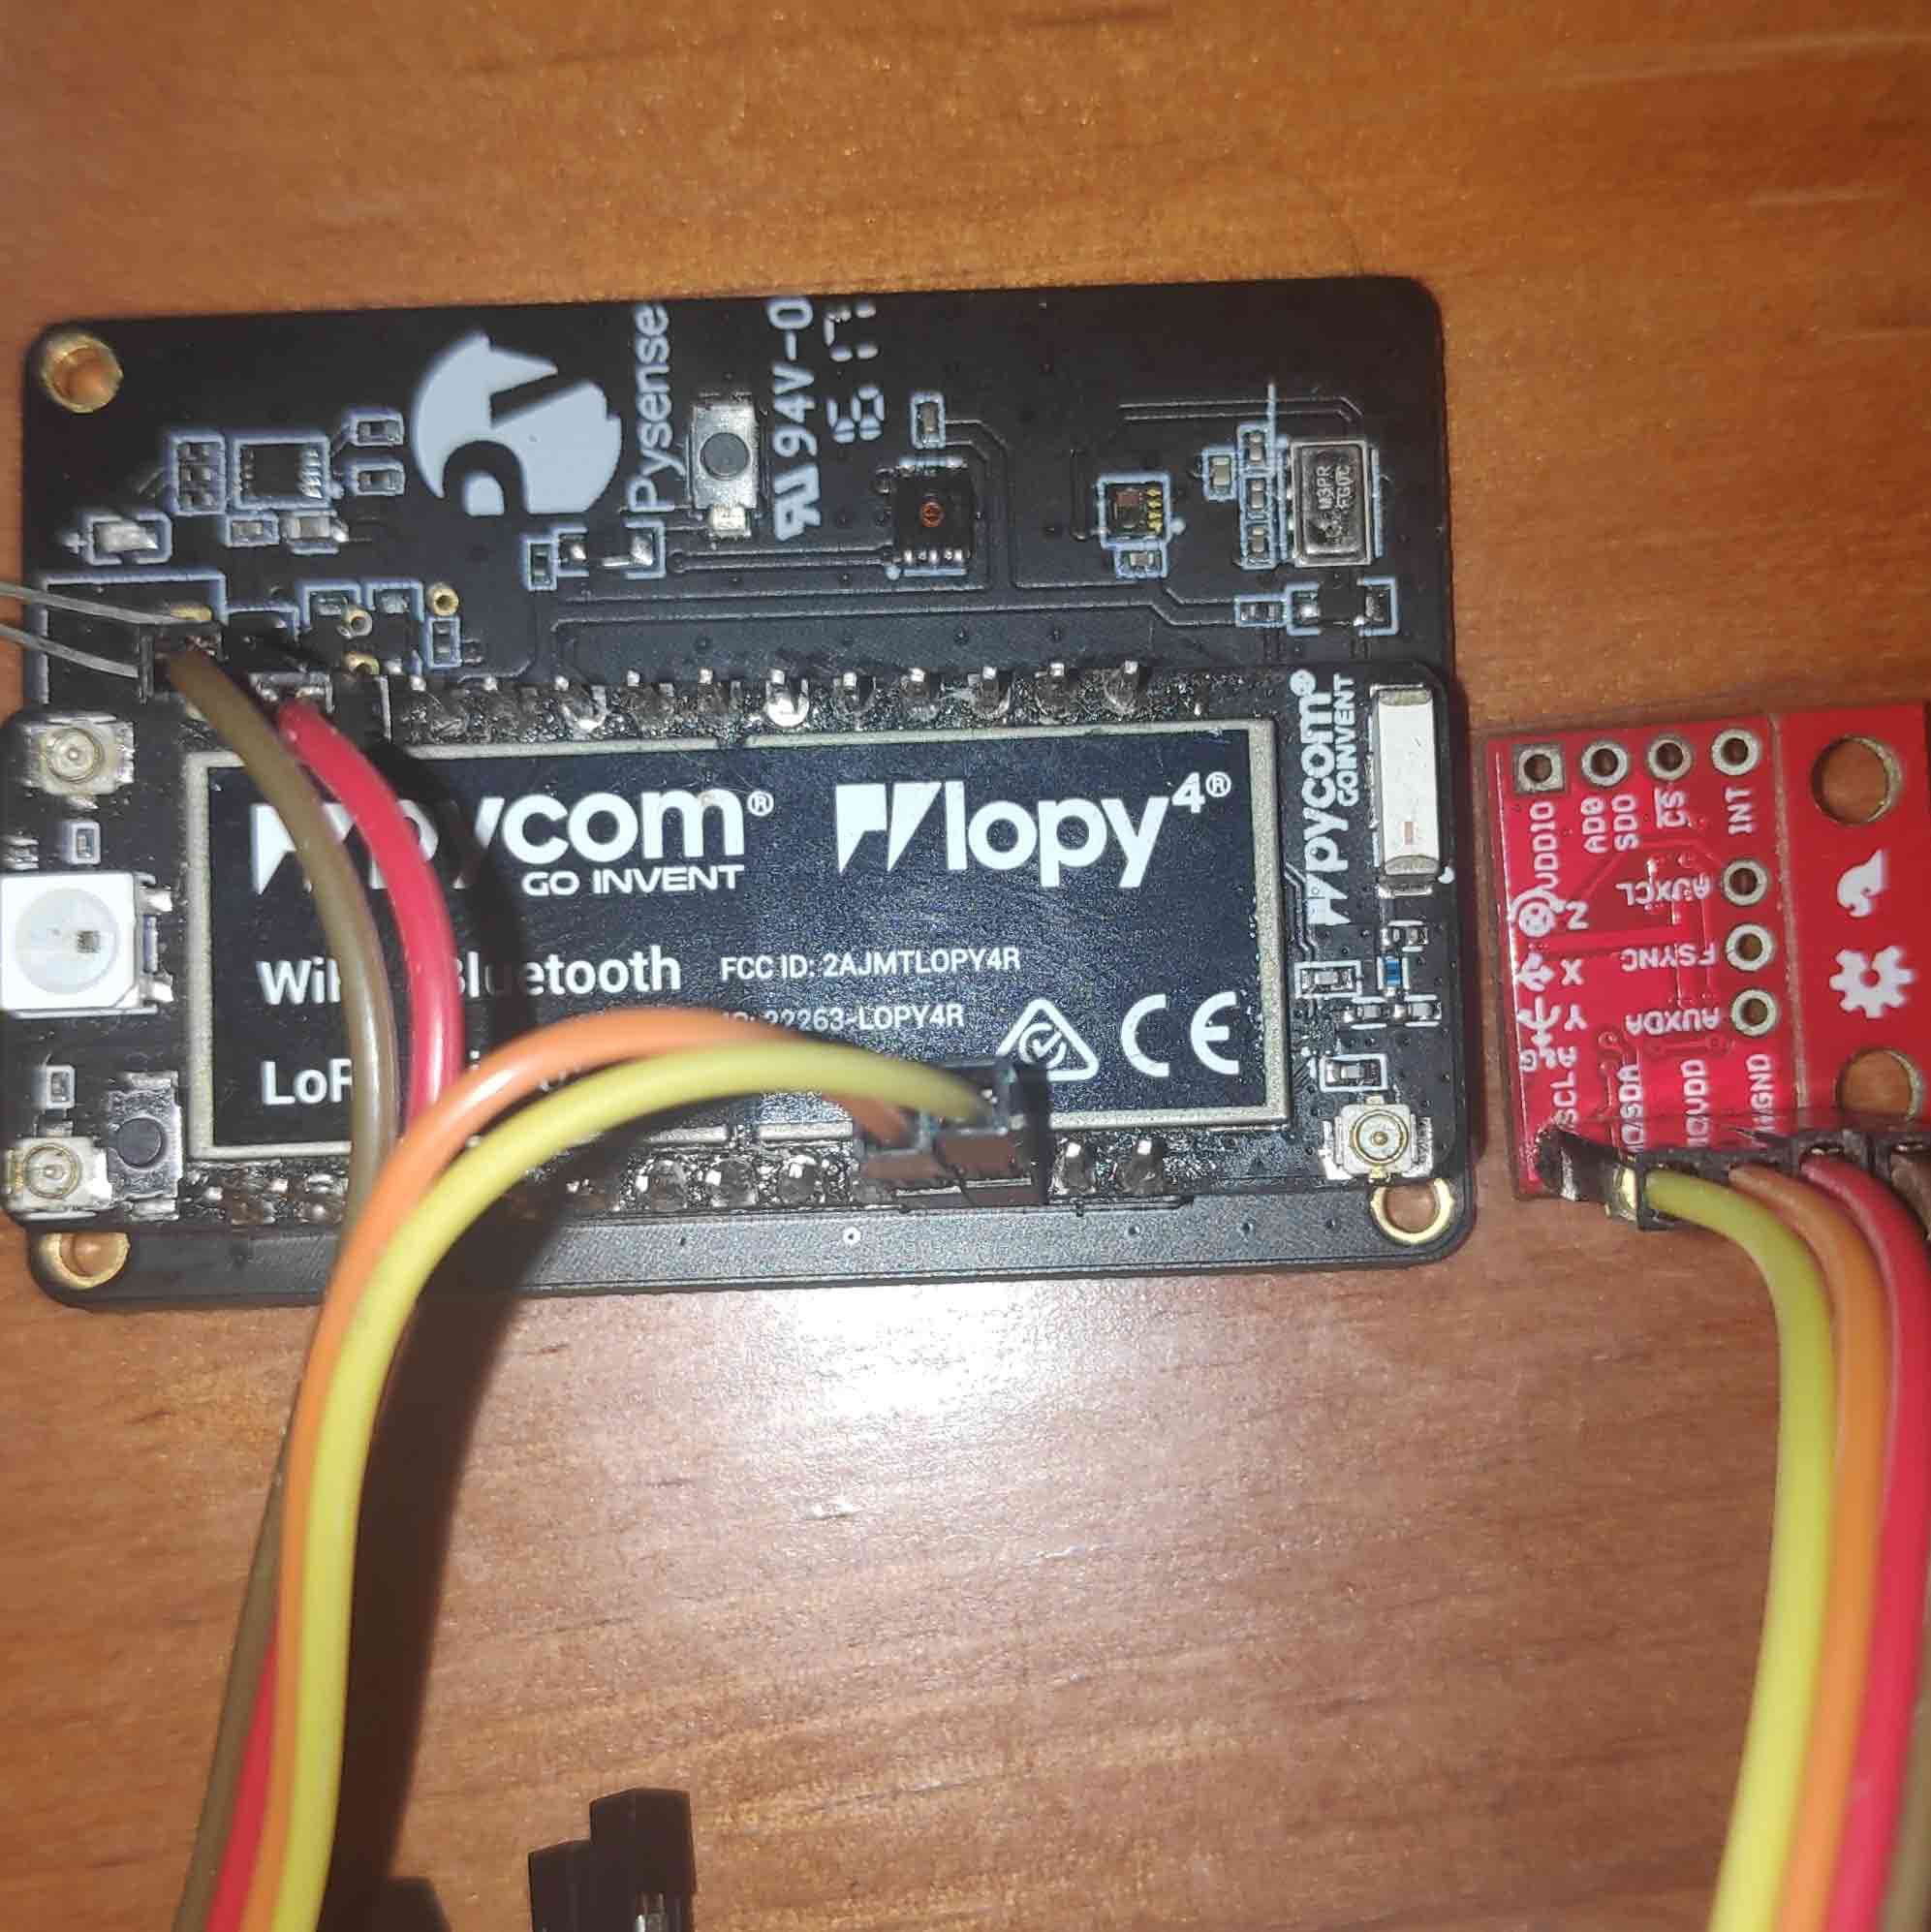
\includegraphics[width=1\textwidth]{figures/INS.jpg}
        \caption{INS Hardware}
        \label{fig:sub1}
    \end{subfigure}%
    \begin{subfigure}{0.25\textwidth}
        \centering
        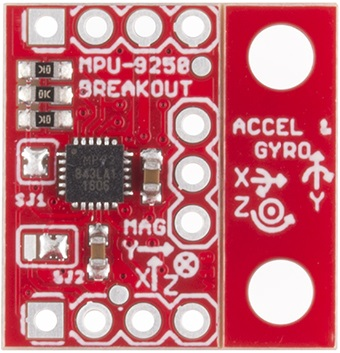
\includegraphics[width=1\textwidth]{figures/mpu9150.jpg}
        \caption{MPU-9250 Breakout}
        \label{fig:sub2}
    \end{subfigure}
    \caption{Pin connection between the microcontroller (left) and the IMU (right). Modules are linked through SCL, CLK, VDD and GND pins.}
    \label{fig:hardware}
\end{figure}

\begin{figure}[!h]
    \centering
    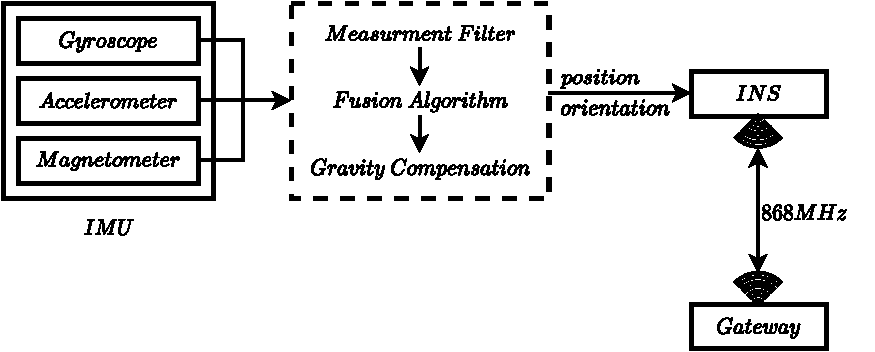
\includegraphics[width=0.475\textwidth]{figures/overview.pdf}
    \caption{System overview - Raw measurements from IMU are fused together and numerically integrated to obtain position and orientation. This INS data is transmitted in real-time to a remote node gateway. }
    \label{fig:overview}
\end{figure}

\begin{figure}[!h]
    \centering
    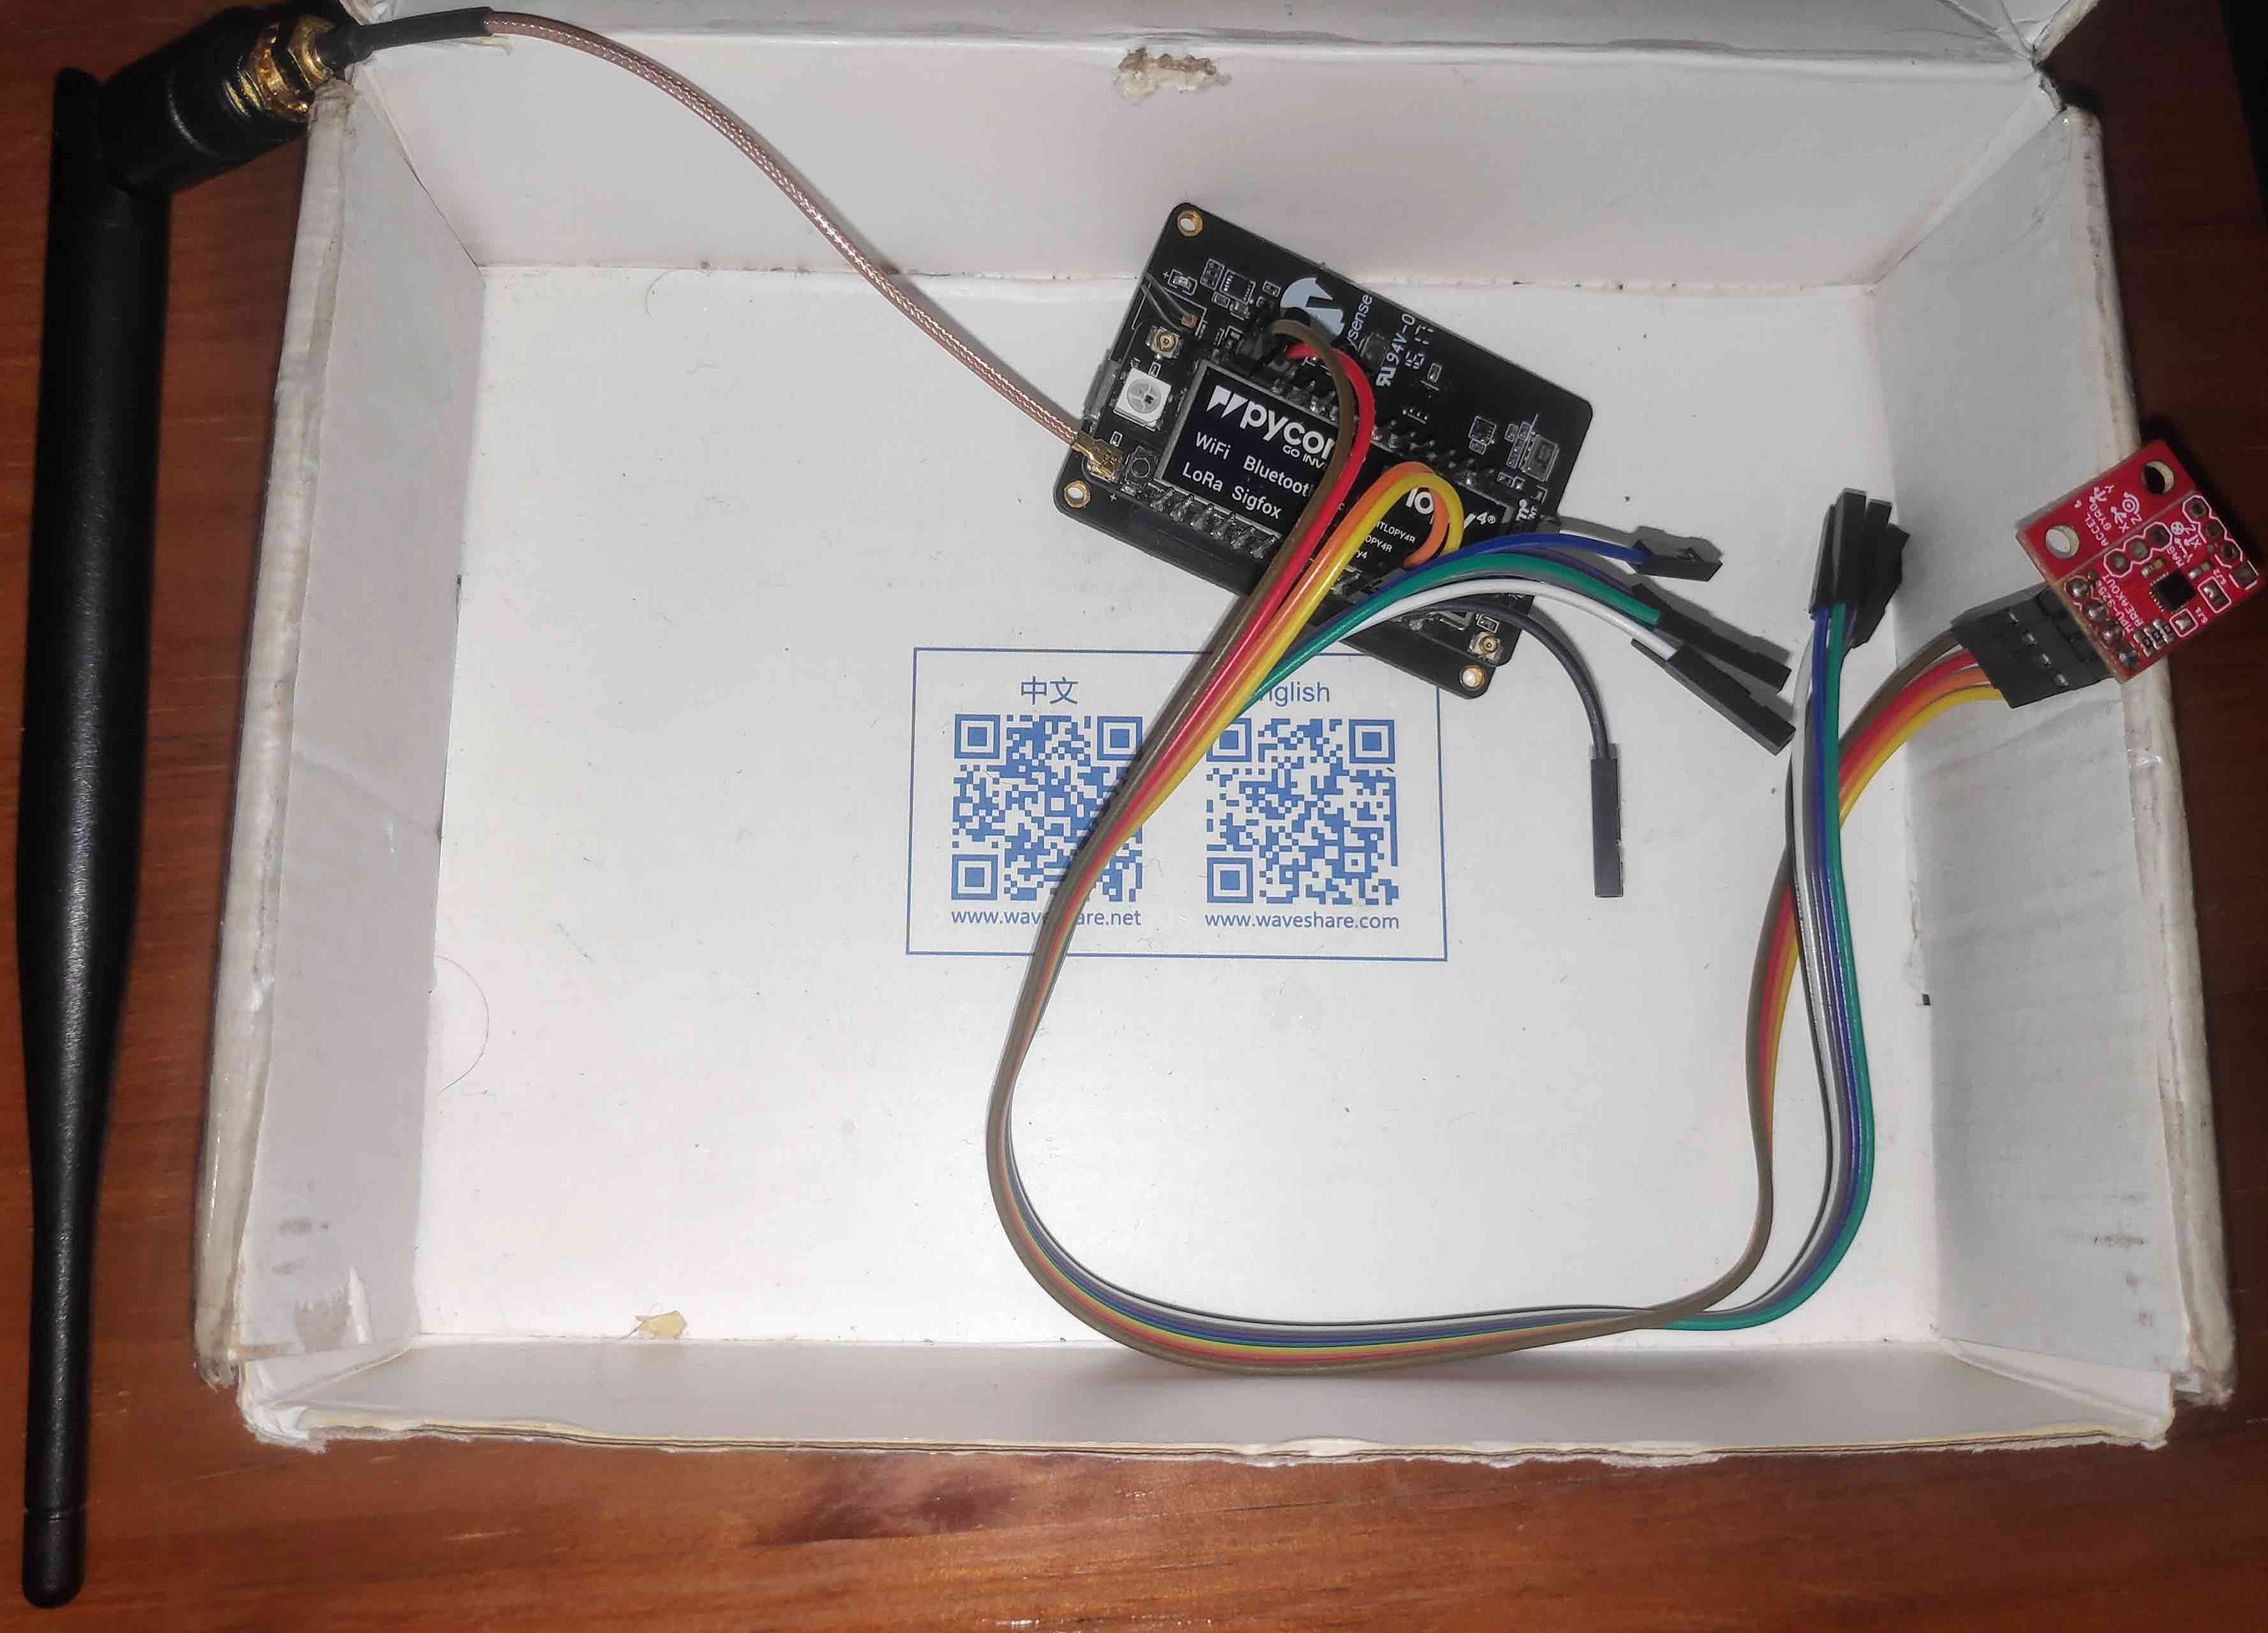
\includegraphics[width=0.475\textwidth]{figures/fullINS.jpg}
    \caption{Complete hardware solution - Box containing the full inertial navigation system, at the left the antenna  suitable for use in the 868MHz/915MHz LoRa bands. }
    \label{fig:full}
\end{figure}
% \onecolumn
% \subsection{Planing (gantt-chart)}
% \subsection{Experiment 1. AHRS on IoT Devices}
% Pitch, Roll, Yaw, 

% \subsection{Experiment 2. Distance Estimation Techniques}
% Position in Euclidean space.
% GPS, Altitude (z), acc -> velocity, velocity -> displacement, with magnetic north

% \subsection{Experiment 3. Comparisons on divers flying units} % balloon, UAV, parasailing


% \subsection{System Architecture}
% \subsection{Software / Algorithms}
% \subsection{Hardware}
